\section{Beam Line and Detectors}
\label{hptpcPaper:sec:Methods}

\subsection{Beam Test Overview}
The beam test took place in the T10 beam line, East Area at the Proton Synchrotron in CERN from the 15th August to the 18th September 2018.
The results in this paper use data taken on the 28th August and 1st September, during which the setup configuration was varied as described below.
\todo[inline]{JOCELYN:"really only these two days?  This paper needs to be the flux reference, so we also need to include the flux measurements during the beam test....
suggest cut this sentence in any case and refer to the time ranges of the various types of data where these are analyzed" SEB what do you think? - SEB: Changed to reflect the increased range of 4 block data used.}
The primary components of the  experimental setup for the data taking period are shown schematically in Figure~\ref{fig:setup}.

\begin{figure}
  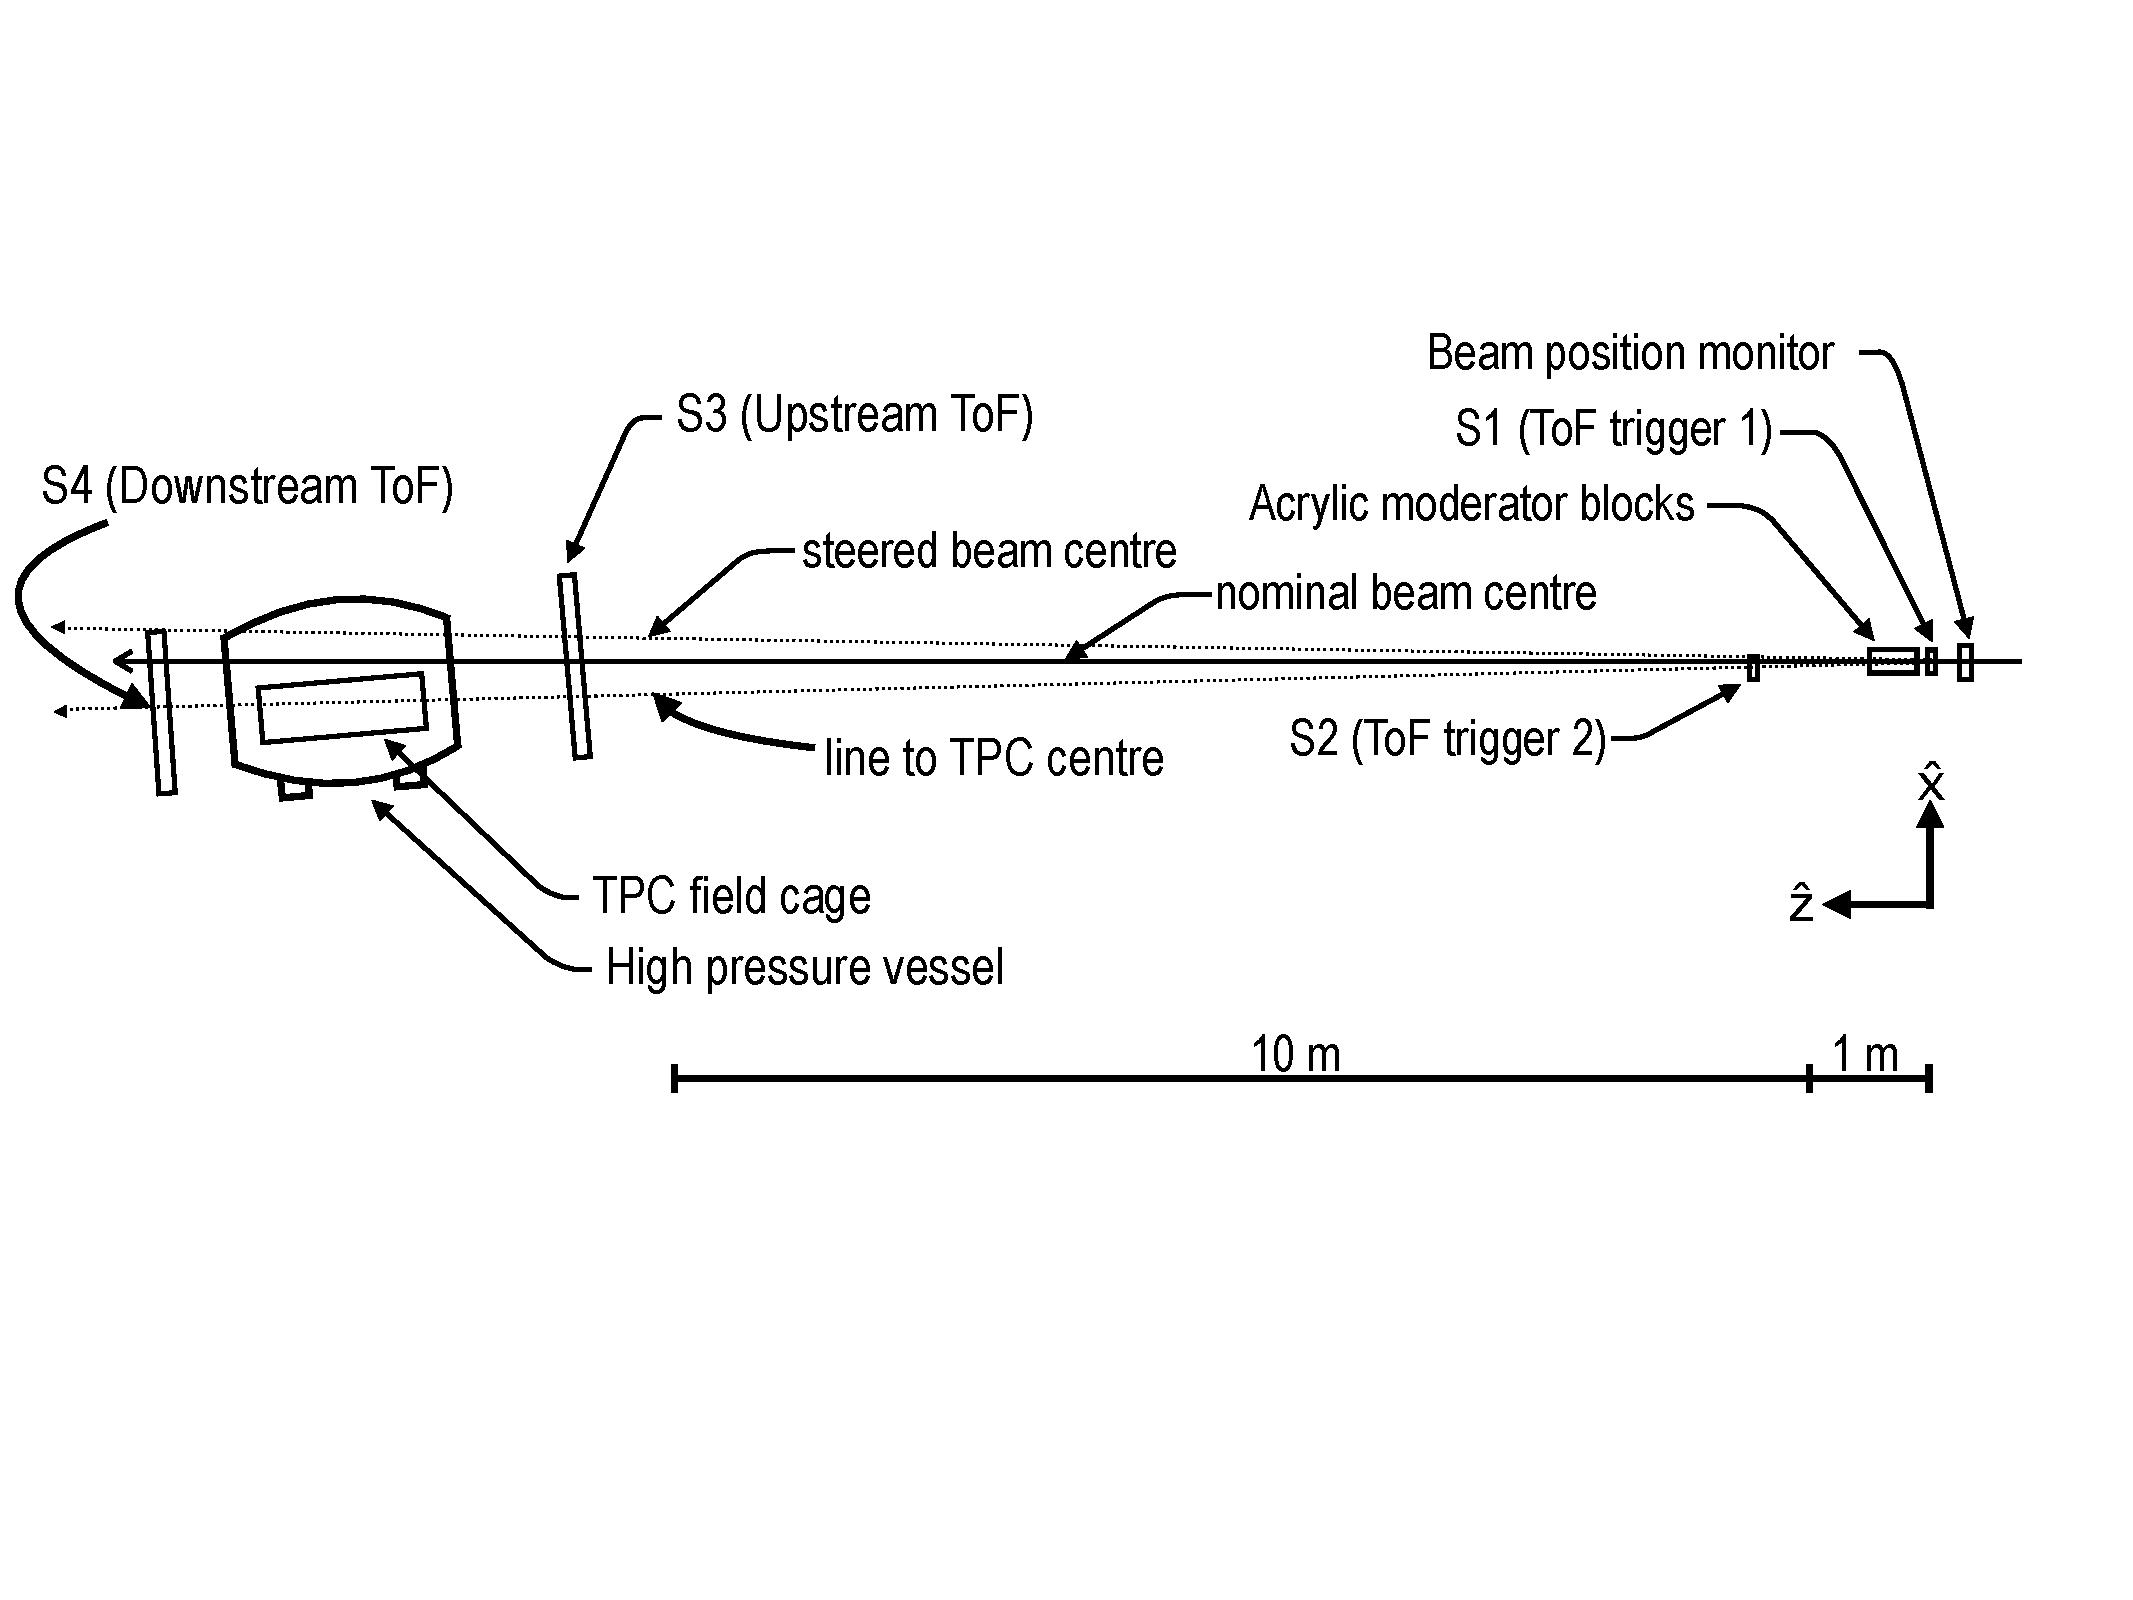
\includegraphics[width=1.0\linewidth]{files/Figures/hptpc_t10_planview.pdf}
  \caption{Beam test configuration}
  \label{fig:setup}
\end{figure}

The T10 beamline at CERN is a secondary beam derived from the Proton Synchrotron beam which consists primarily of protons, electrons and charged pions~\cite{T10Report}.

The beam position monitor lies upstream of all the ToF constituents and the TPC, at the beam entrance. 
%The centre of the HPTPC Prototype was placed 13~m from the wire chamber at the beam entrance. 
The beam position monitor is followed by three ToF constituents: $\mathit{S1}$, which provides the trigger is a small-area beam trigger.
$\mathit{S2}$, a trigger counter that provides a coincidence measurement with $\mathit{S1}$.
$\mathit{S3}$, a large wall of plastic scintillator bars, placed directly upstream of the TPC vessel.
All three of these upstream constituents are described in greater detail in Sections~\ref{subsec:s1s2Exp}~and~\ref{subsec:s3Exp}.
Directly between $\mathit{S1}$ and $\mathit{S2}$, a variable number of blocks of acrylic moderator were placed, and are shown in Figure~\ref{fig:modblocks}.
The vessel containing the TPC was placed 13~m from the wire chamber at the beam entrance.
Lastly, a fourth ToF constituent, labeled $\mathit{S4}$, was placed directly downstream of the vessel.
This was a second wall of plastic scintillator bars, described further in Section~\ref{subsec:s4Exp}.
Both the TPC and ToF systems were placed at an off-axis angle with respect to the direction of the beam.
To study the impact of moderator thickness, a variable number of blocks of acrylic, each of dimension $10\times10\times10$~cm$^3$, were placed in the beamline, with the upstream end of the moderators located xxx cm behind $\mathit{S1}$, and are shown in Figure~\ref{fig:modblocks}.

\todo[inline]{also need the off axis angle (with +/-). Need to check the mod block from S1}

Data acquisition (DAQ) of up- and downstream ToF systems were completely independent.
The synchronization between systems was performed offline using the reference signal from the PS at the beginning of every spill.
The PS beam structure is as follows: T10 received between 1 and 3 spills during each supercycle which has a typical duration of 33~s.
The spill duration is approximately 400~ms.
The minimum separation in time between two spills is approximately 1 second.
Therefore the start of spill signal frequency is 1 Hz or smaller.
The trigger condition of the upstream ToF was based on the coincidence between $\mathit{S1}$ and $\mathit{S3}$ constituents.
$\mathit{S2}$ signals were also recorded but the upstream ToF DAQ but were not a trigger condition.
The DAQ of the downstream ToF, $\mathit{S4}$, was run in self-triggering mode with a gate open during the spill.
Coincidence signals between $\mathit{S1}$ and $\mathit{S2}$ counters were also recorded by the downstream ToF DAQ and were used in the particle identification (PID) analysis, described in Section~\ref{hptpcPaper:sec:Results}.  

A system of moderator blocks was located between the $\mathit{S1}$ and $\mathit{S2}$ counters.
The system was composed of a stand on which up to four polystyrene $10\times10\times10$~cm$^3$ blocks could be placed contiguously.
Figure~\ref{fig:modblocks} shows the stand with four blocks installed.
The moderator blocks have the effect of both reducing the energy of incoming particles as well as scattering protons in the beam through higher angles than beam MIPs.
This tends to increase the proton-to-MIP ratio at low off-axis angles from the beam, while decreasing the total number of protons and MIPs traversing the TPC.
A maximum of four moderator blocks was chosen to retain a minimum intensity in the TPC.
%The addition of too many moderator blocks would cause an overscattering whereby too many protons fall below threshold as compared with MIPs.

Data was taken with the beam momentum primarily at 0.8~GeV/c, and with each configuration of 0 to 4 moderator blocks.
%Figure~INSERT shows the typical composition of the beam upstream of $\mathit{S1}$ at 0.8~GeV/c. Beam spills were approximately 500~ms in length with 5-10~s between spills.  
\todo[inline]{JOCELYN:"In general, you need a paragraph and a figure or two that describe the T10 beam before you do anything to it. The description of the un-modified beam should come before any explanation about the modifications, so probably as a subsection at the end of section 1. This unmodified beam data should probably come from the 2016 measurements, or the on-axis TOF measurements with no moderator." - similar to previous comment 2016 data probably best So maybe remove figure INSERT, and just do a subsection at the end of section 1.}

%    Moderator blocks were used in order to cause a spread in the incoming beam.
%    The blocks cause protons to scatter through a larger angle than pions and other minimum ionising particles (MIP), increasing the off-axis proton pion ratio.
%    The effect of this, together with placing the TPC and ToF systems off axis was to allow a measurement of protons with a lower pion background.
%    This technique also had the effect of reducing the average momentum of the measured particles.
%    Data were taken for 0, 1, 2, 3, and 4 moderator blocks in turn.
%    The beam ran with an energy of 0.8~GeV/c, and primarily comprised protons and pions, as well as muons and electrons. 
%    Beam spills were approximately 500~ms in length, with 5-10~s between spills.
%    The ratio of protons to pions expected in the T10 beam  is shown in figure~\ref{beamcharacteristics}.
%    From this figure, the expected on axis proton pion ratio at 0.8~GeV/c is approximately 1:6.
%      \begin{figure}
%      \centering
%    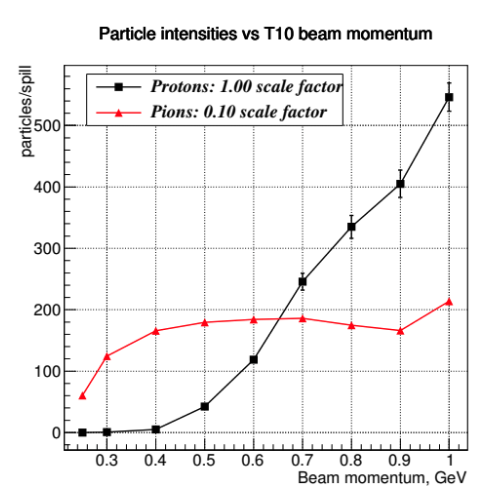
\includegraphics[width=0.6\linewidth]{files/Figures/offaxismeasurement.png}
%    	\caption{T10 beam constituents (REFERENCE NEEDED)}
%    		\label{fig:beamcharacteristics}
%    \end{figure}


\begin{figure}[t]
  \centering
  %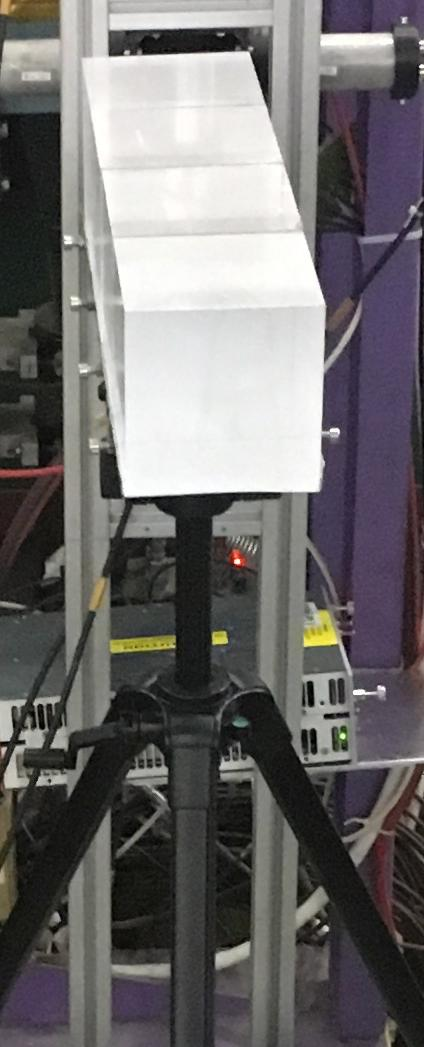
\includegraphics[width=0.2\linewidth]{files/Figures/ModeratorBlocks.jpg}
  \includegraphics[width=1.05\linewidth]{files/Figures/S1S2S3S4.png}
  \caption{Photo demonstrating the $\mathit{S1}$ and $\mathit{S2}$ counters and the stand with four acrylic moderator blocks of the upstream part of the setup (right). Photo of the downstream part of the setup which shows the $\mathit{S3}$, $\mathit{S4}$ detectors and HPTPC (left).}
  \label{fig:modblocks}
\end{figure}

\subsection{Survey and coordinate system}
\label{sec:coord}
The T10 beamline area is surveyed and the distances to various components measured to a precision of 0.5~mm by the CERN Survey, Mechatronics and Measurements (SMM) group.
These measurements are used to calculate the positions of various components in the beamline relative to one another.
Multiple points on each of $\mathit{S1}$, $\mathit{S2}$, $\mathit{S3}$, $\mathit{S4}$ and the TPC frame have their positions measured relative to an origin located at the nominal T10 beam focussing point.

The off-axis angles, $\theta$ and $\phi$, are defined using the axes shown in Figure~\ref{fig:setup}.
The origin is taken to be at $\mathit{S1}$.
The horizontal off-axis angle, $\theta$, is defined as the angle in the $x-z$ plane as shown in Figure~\ref{fig:setup} with $\theta = 0^{\circ}$ parallel to the $z$ axis and with positive $\theta$ in the negative $x$ direction.
The vertical off-axis angle, $\phi$, is defined as the angle between the $z$ axis and the vertical.
$\phi = 0^{\circ}$ is parallel to the $z$ axis.
$\phi$ increases with increasing vertical position.

Figure~\ref{fig:angularDistS1} shows the angular distribution of various objects within the beamline using the coordinate system defined above. Table~\ref{tab:angS1} shows the calculated angular extent of the various beamline components as measured from $\mathit{S1}$.

\begin{figure}[ht]
  \begin{adjustbox}{max totalsize={0.7\textwidth}{.5\textheight},center}
    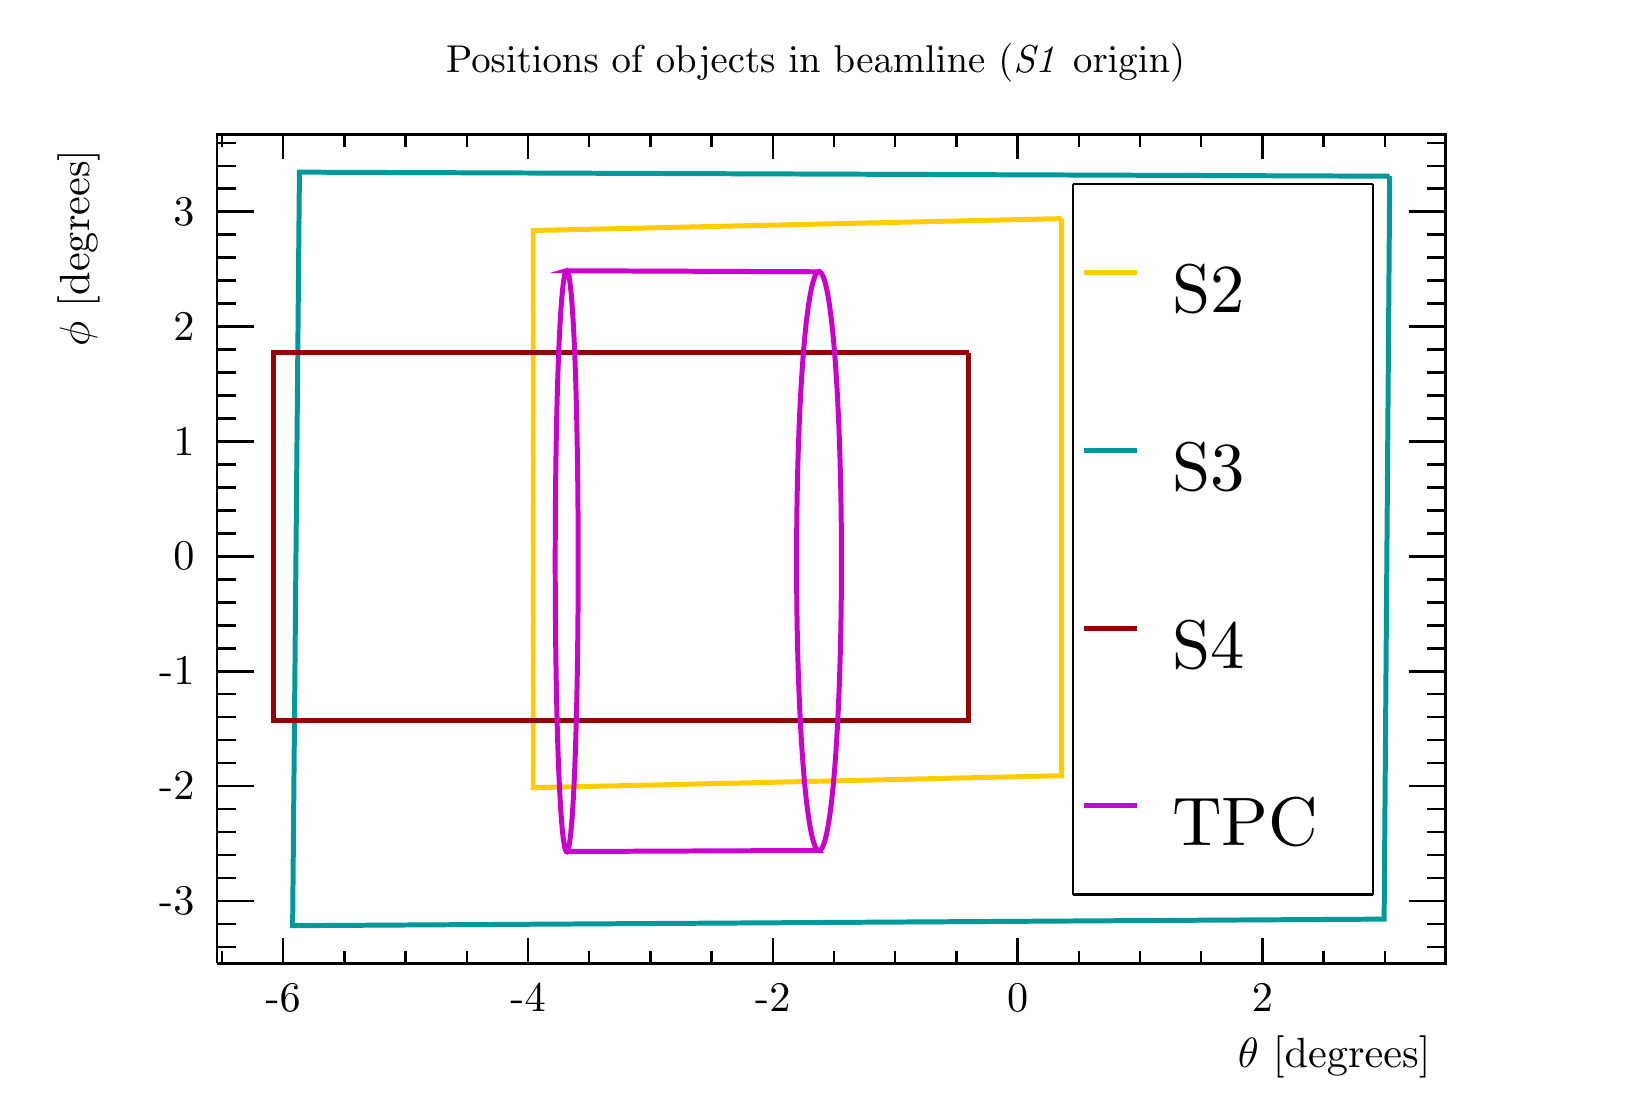
\begin{tikzpicture}
\pgfdeclareplotmark{cross} {
\pgfpathmoveto{\pgfpoint{-0.3\pgfplotmarksize}{\pgfplotmarksize}}
\pgfpathlineto{\pgfpoint{+0.3\pgfplotmarksize}{\pgfplotmarksize}}
\pgfpathlineto{\pgfpoint{+0.3\pgfplotmarksize}{0.3\pgfplotmarksize}}
\pgfpathlineto{\pgfpoint{+1\pgfplotmarksize}{0.3\pgfplotmarksize}}
\pgfpathlineto{\pgfpoint{+1\pgfplotmarksize}{-0.3\pgfplotmarksize}}
\pgfpathlineto{\pgfpoint{+0.3\pgfplotmarksize}{-0.3\pgfplotmarksize}}
\pgfpathlineto{\pgfpoint{+0.3\pgfplotmarksize}{-1.\pgfplotmarksize}}
\pgfpathlineto{\pgfpoint{-0.3\pgfplotmarksize}{-1.\pgfplotmarksize}}
\pgfpathlineto{\pgfpoint{-0.3\pgfplotmarksize}{-0.3\pgfplotmarksize}}
\pgfpathlineto{\pgfpoint{-1.\pgfplotmarksize}{-0.3\pgfplotmarksize}}
\pgfpathlineto{\pgfpoint{-1.\pgfplotmarksize}{0.3\pgfplotmarksize}}
\pgfpathlineto{\pgfpoint{-0.3\pgfplotmarksize}{0.3\pgfplotmarksize}}
\pgfpathclose
\pgfusepathqstroke
}
\pgfdeclareplotmark{cross*} {
\pgfpathmoveto{\pgfpoint{-0.3\pgfplotmarksize}{\pgfplotmarksize}}
\pgfpathlineto{\pgfpoint{+0.3\pgfplotmarksize}{\pgfplotmarksize}}
\pgfpathlineto{\pgfpoint{+0.3\pgfplotmarksize}{0.3\pgfplotmarksize}}
\pgfpathlineto{\pgfpoint{+1\pgfplotmarksize}{0.3\pgfplotmarksize}}
\pgfpathlineto{\pgfpoint{+1\pgfplotmarksize}{-0.3\pgfplotmarksize}}
\pgfpathlineto{\pgfpoint{+0.3\pgfplotmarksize}{-0.3\pgfplotmarksize}}
\pgfpathlineto{\pgfpoint{+0.3\pgfplotmarksize}{-1.\pgfplotmarksize}}
\pgfpathlineto{\pgfpoint{-0.3\pgfplotmarksize}{-1.\pgfplotmarksize}}
\pgfpathlineto{\pgfpoint{-0.3\pgfplotmarksize}{-0.3\pgfplotmarksize}}
\pgfpathlineto{\pgfpoint{-1.\pgfplotmarksize}{-0.3\pgfplotmarksize}}
\pgfpathlineto{\pgfpoint{-1.\pgfplotmarksize}{0.3\pgfplotmarksize}}
\pgfpathlineto{\pgfpoint{-0.3\pgfplotmarksize}{0.3\pgfplotmarksize}}
\pgfpathclose
\pgfusepathqfillstroke
}
\pgfdeclareplotmark{newstar} {
\pgfpathmoveto{\pgfqpoint{0pt}{\pgfplotmarksize}}
\pgfpathlineto{\pgfqpointpolar{44}{0.5\pgfplotmarksize}}
\pgfpathlineto{\pgfqpointpolar{18}{\pgfplotmarksize}}
\pgfpathlineto{\pgfqpointpolar{-20}{0.5\pgfplotmarksize}}
\pgfpathlineto{\pgfqpointpolar{-54}{\pgfplotmarksize}}
\pgfpathlineto{\pgfqpointpolar{-90}{0.5\pgfplotmarksize}}
\pgfpathlineto{\pgfqpointpolar{234}{\pgfplotmarksize}}
\pgfpathlineto{\pgfqpointpolar{198}{0.5\pgfplotmarksize}}
\pgfpathlineto{\pgfqpointpolar{162}{\pgfplotmarksize}}
\pgfpathlineto{\pgfqpointpolar{134}{0.5\pgfplotmarksize}}
\pgfpathclose
\pgfusepathqstroke
}
\pgfdeclareplotmark{newstar*} {
\pgfpathmoveto{\pgfqpoint{0pt}{\pgfplotmarksize}}
\pgfpathlineto{\pgfqpointpolar{44}{0.5\pgfplotmarksize}}
\pgfpathlineto{\pgfqpointpolar{18}{\pgfplotmarksize}}
\pgfpathlineto{\pgfqpointpolar{-20}{0.5\pgfplotmarksize}}
\pgfpathlineto{\pgfqpointpolar{-54}{\pgfplotmarksize}}
\pgfpathlineto{\pgfqpointpolar{-90}{0.5\pgfplotmarksize}}
\pgfpathlineto{\pgfqpointpolar{234}{\pgfplotmarksize}}
\pgfpathlineto{\pgfqpointpolar{198}{0.5\pgfplotmarksize}}
\pgfpathlineto{\pgfqpointpolar{162}{\pgfplotmarksize}}
\pgfpathlineto{\pgfqpointpolar{134}{0.5\pgfplotmarksize}}
\pgfpathclose
\pgfusepathqfillstroke
}
\definecolor{c}{rgb}{1,1,1};
\draw [color=c, fill=c] (0,0) rectangle (20,13.4957);
\draw [color=c, fill=c] (2.4,1.61948) rectangle (18,12.1461);
\definecolor{c}{rgb}{0,0,0};
\draw [c,line width=0.9] (2.4,1.61948) -- (2.4,12.1461) -- (18,12.1461) -- (18,1.61948) -- (2.4,1.61948);
\definecolor{c}{rgb}{1,1,1};
\draw [color=c, fill=c] (2.4,1.61948) rectangle (18,12.1461);
\definecolor{c}{rgb}{0,0,0};
\draw [c,line width=0.9] (2.4,1.61948) -- (2.4,12.1461) -- (18,12.1461) -- (18,1.61948) -- (2.4,1.61948);
\draw [c,line width=0.9] (2.4,1.61948) -- (18,1.61948);
\draw [c,line width=0.9] (3.23864,1.93528) -- (3.23864,1.61948);
\draw [c,line width=0.9] (4.01586,1.77738) -- (4.01586,1.61948);
\draw [c,line width=0.9] (4.79308,1.77738) -- (4.79308,1.61948);
\draw [c,line width=0.9] (5.5703,1.77738) -- (5.5703,1.61948);
\draw [c,line width=0.9] (6.34753,1.93528) -- (6.34753,1.61948);
\draw [c,line width=0.9] (7.12475,1.77738) -- (7.12475,1.61948);
\draw [c,line width=0.9] (7.90197,1.77738) -- (7.90197,1.61948);
\draw [c,line width=0.9] (8.67919,1.77738) -- (8.67919,1.61948);
\draw [c,line width=0.9] (9.45641,1.93528) -- (9.45641,1.61948);
\draw [c,line width=0.9] (10.2336,1.77738) -- (10.2336,1.61948);
\draw [c,line width=0.9] (11.0109,1.77738) -- (11.0109,1.61948);
\draw [c,line width=0.9] (11.7881,1.77738) -- (11.7881,1.61948);
\draw [c,line width=0.9] (12.5653,1.93528) -- (12.5653,1.61948);
\draw [c,line width=0.9] (13.3425,1.77738) -- (13.3425,1.61948);
\draw [c,line width=0.9] (14.1197,1.77738) -- (14.1197,1.61948);
\draw [c,line width=0.9] (14.897,1.77738) -- (14.897,1.61948);
\draw [c,line width=0.9] (15.6742,1.93528) -- (15.6742,1.61948);
\draw [c,line width=0.9] (3.23864,1.93528) -- (3.23864,1.61948);
\draw [c,line width=0.9] (2.46142,1.77738) -- (2.46142,1.61948);
\draw [c,line width=0.9] (15.6742,1.93528) -- (15.6742,1.61948);
\draw [c,line width=0.9] (16.4514,1.77738) -- (16.4514,1.61948);
\draw [c,line width=0.9] (17.2286,1.77738) -- (17.2286,1.61948);
\draw [anchor=base] (3.23864,1.01218) node[scale=1.52731, color=c, rotate=0]{-6};
\draw [anchor=base] (6.34753,1.01218) node[scale=1.52731, color=c, rotate=0]{-4};
\draw [anchor=base] (9.45641,1.01218) node[scale=1.52731, color=c, rotate=0]{-2};
\draw [anchor=base] (12.5653,1.01218) node[scale=1.52731, color=c, rotate=0]{0};
\draw [anchor=base] (15.6742,1.01218) node[scale=1.52731, color=c, rotate=0]{2};
\draw [anchor= east] (18,0.431862) node[scale=1.52731, color=c, rotate=0]{$ \theta$ [degrees]};
\draw [c,line width=0.9] (2.4,12.1461) -- (18,12.1461);
\draw [c,line width=0.9] (3.23864,11.8303) -- (3.23864,12.1461);
\draw [c,line width=0.9] (4.01586,11.9882) -- (4.01586,12.1461);
\draw [c,line width=0.9] (4.79308,11.9882) -- (4.79308,12.1461);
\draw [c,line width=0.9] (5.5703,11.9882) -- (5.5703,12.1461);
\draw [c,line width=0.9] (6.34753,11.8303) -- (6.34753,12.1461);
\draw [c,line width=0.9] (7.12475,11.9882) -- (7.12475,12.1461);
\draw [c,line width=0.9] (7.90197,11.9882) -- (7.90197,12.1461);
\draw [c,line width=0.9] (8.67919,11.9882) -- (8.67919,12.1461);
\draw [c,line width=0.9] (9.45641,11.8303) -- (9.45641,12.1461);
\draw [c,line width=0.9] (10.2336,11.9882) -- (10.2336,12.1461);
\draw [c,line width=0.9] (11.0109,11.9882) -- (11.0109,12.1461);
\draw [c,line width=0.9] (11.7881,11.9882) -- (11.7881,12.1461);
\draw [c,line width=0.9] (12.5653,11.8303) -- (12.5653,12.1461);
\draw [c,line width=0.9] (13.3425,11.9882) -- (13.3425,12.1461);
\draw [c,line width=0.9] (14.1197,11.9882) -- (14.1197,12.1461);
\draw [c,line width=0.9] (14.897,11.9882) -- (14.897,12.1461);
\draw [c,line width=0.9] (15.6742,11.8303) -- (15.6742,12.1461);
\draw [c,line width=0.9] (3.23864,11.8303) -- (3.23864,12.1461);
\draw [c,line width=0.9] (2.46142,11.9882) -- (2.46142,12.1461);
\draw [c,line width=0.9] (15.6742,11.8303) -- (15.6742,12.1461);
\draw [c,line width=0.9] (16.4514,11.9882) -- (16.4514,12.1461);
\draw [c,line width=0.9] (17.2286,11.9882) -- (17.2286,12.1461);
\draw [c,line width=0.9] (2.4,1.61948) -- (2.4,12.1461);
\draw [c,line width=0.9] (2.868,2.41096) -- (2.4,2.41096);
\draw [c,line width=0.9] (2.634,2.70278) -- (2.4,2.70278);
\draw [c,line width=0.9] (2.634,2.99459) -- (2.4,2.99459);
\draw [c,line width=0.9] (2.634,3.28641) -- (2.4,3.28641);
\draw [c,line width=0.9] (2.634,3.57822) -- (2.4,3.57822);
\draw [c,line width=0.9] (2.868,3.87004) -- (2.4,3.87004);
\draw [c,line width=0.9] (2.634,4.16185) -- (2.4,4.16185);
\draw [c,line width=0.9] (2.634,4.45367) -- (2.4,4.45367);
\draw [c,line width=0.9] (2.634,4.74548) -- (2.4,4.74548);
\draw [c,line width=0.9] (2.634,5.0373) -- (2.4,5.0373);
\draw [c,line width=0.9] (2.868,5.32911) -- (2.4,5.32911);
\draw [c,line width=0.9] (2.634,5.62093) -- (2.4,5.62093);
\draw [c,line width=0.9] (2.634,5.91274) -- (2.4,5.91274);
\draw [c,line width=0.9] (2.634,6.20456) -- (2.4,6.20456);
\draw [c,line width=0.9] (2.634,6.49638) -- (2.4,6.49638);
\draw [c,line width=0.9] (2.868,6.78819) -- (2.4,6.78819);
\draw [c,line width=0.9] (2.634,7.08001) -- (2.4,7.08001);
\draw [c,line width=0.9] (2.634,7.37182) -- (2.4,7.37182);
\draw [c,line width=0.9] (2.634,7.66364) -- (2.4,7.66364);
\draw [c,line width=0.9] (2.634,7.95545) -- (2.4,7.95545);
\draw [c,line width=0.9] (2.868,8.24727) -- (2.4,8.24727);
\draw [c,line width=0.9] (2.634,8.53908) -- (2.4,8.53908);
\draw [c,line width=0.9] (2.634,8.8309) -- (2.4,8.8309);
\draw [c,line width=0.9] (2.634,9.12271) -- (2.4,9.12271);
\draw [c,line width=0.9] (2.634,9.41453) -- (2.4,9.41453);
\draw [c,line width=0.9] (2.868,9.70634) -- (2.4,9.70634);
\draw [c,line width=0.9] (2.634,9.99816) -- (2.4,9.99816);
\draw [c,line width=0.9] (2.634,10.29) -- (2.4,10.29);
\draw [c,line width=0.9] (2.634,10.5818) -- (2.4,10.5818);
\draw [c,line width=0.9] (2.634,10.8736) -- (2.4,10.8736);
\draw [c,line width=0.9] (2.868,11.1654) -- (2.4,11.1654);
\draw [c,line width=0.9] (2.868,2.41096) -- (2.4,2.41096);
\draw [c,line width=0.9] (2.634,2.11915) -- (2.4,2.11915);
\draw [c,line width=0.9] (2.634,1.82733) -- (2.4,1.82733);
\draw [c,line width=0.9] (2.868,11.1654) -- (2.4,11.1654);
\draw [c,line width=0.9] (2.634,11.4572) -- (2.4,11.4572);
\draw [c,line width=0.9] (2.634,11.749) -- (2.4,11.749);
\draw [c,line width=0.9] (2.634,12.0409) -- (2.4,12.0409);
\draw [anchor= east] (2.3,2.41096) node[scale=1.52731, color=c, rotate=0]{-3};
\draw [anchor= east] (2.3,3.87004) node[scale=1.52731, color=c, rotate=0]{-2};
\draw [anchor= east] (2.3,5.32911) node[scale=1.52731, color=c, rotate=0]{-1};
\draw [anchor= east] (2.3,6.78819) node[scale=1.52731, color=c, rotate=0]{0};
\draw [anchor= east] (2.3,8.24727) node[scale=1.52731, color=c, rotate=0]{1};
\draw [anchor= east] (2.3,9.70634) node[scale=1.52731, color=c, rotate=0]{2};
\draw [anchor= east] (2.3,11.1654) node[scale=1.52731, color=c, rotate=0]{3};
\draw [anchor= east] (0.64,12.1461) node[scale=1.52731, color=c, rotate=90]{$ \phi$ [degrees]};
\draw [c,line width=0.9] (18,1.61948) -- (18,12.1461);
\draw [c,line width=0.9] (17.532,2.41096) -- (18,2.41096);
\draw [c,line width=0.9] (17.766,2.70278) -- (18,2.70278);
\draw [c,line width=0.9] (17.766,2.99459) -- (18,2.99459);
\draw [c,line width=0.9] (17.766,3.28641) -- (18,3.28641);
\draw [c,line width=0.9] (17.766,3.57822) -- (18,3.57822);
\draw [c,line width=0.9] (17.532,3.87004) -- (18,3.87004);
\draw [c,line width=0.9] (17.766,4.16185) -- (18,4.16185);
\draw [c,line width=0.9] (17.766,4.45367) -- (18,4.45367);
\draw [c,line width=0.9] (17.766,4.74548) -- (18,4.74548);
\draw [c,line width=0.9] (17.766,5.0373) -- (18,5.0373);
\draw [c,line width=0.9] (17.532,5.32911) -- (18,5.32911);
\draw [c,line width=0.9] (17.766,5.62093) -- (18,5.62093);
\draw [c,line width=0.9] (17.766,5.91274) -- (18,5.91274);
\draw [c,line width=0.9] (17.766,6.20456) -- (18,6.20456);
\draw [c,line width=0.9] (17.766,6.49638) -- (18,6.49638);
\draw [c,line width=0.9] (17.532,6.78819) -- (18,6.78819);
\draw [c,line width=0.9] (17.766,7.08001) -- (18,7.08001);
\draw [c,line width=0.9] (17.766,7.37182) -- (18,7.37182);
\draw [c,line width=0.9] (17.766,7.66364) -- (18,7.66364);
\draw [c,line width=0.9] (17.766,7.95545) -- (18,7.95545);
\draw [c,line width=0.9] (17.532,8.24727) -- (18,8.24727);
\draw [c,line width=0.9] (17.766,8.53908) -- (18,8.53908);
\draw [c,line width=0.9] (17.766,8.8309) -- (18,8.8309);
\draw [c,line width=0.9] (17.766,9.12271) -- (18,9.12271);
\draw [c,line width=0.9] (17.766,9.41453) -- (18,9.41453);
\draw [c,line width=0.9] (17.532,9.70634) -- (18,9.70634);
\draw [c,line width=0.9] (17.766,9.99816) -- (18,9.99816);
\draw [c,line width=0.9] (17.766,10.29) -- (18,10.29);
\draw [c,line width=0.9] (17.766,10.5818) -- (18,10.5818);
\draw [c,line width=0.9] (17.766,10.8736) -- (18,10.8736);
\draw [c,line width=0.9] (17.532,11.1654) -- (18,11.1654);
\draw [c,line width=0.9] (17.532,2.41096) -- (18,2.41096);
\draw [c,line width=0.9] (17.766,2.11915) -- (18,2.11915);
\draw [c,line width=0.9] (17.766,1.82733) -- (18,1.82733);
\draw [c,line width=0.9] (17.532,11.1654) -- (18,11.1654);
\draw [c,line width=0.9] (17.766,11.4572) -- (18,11.4572);
\draw [c,line width=0.9] (17.766,11.749) -- (18,11.749);
\draw [c,line width=0.9] (17.766,12.0409) -- (18,12.0409);
\definecolor{c}{rgb}{1,0.8,0};
\draw [c,line width=1.8] (13.123,11.0775) -- (13.123,4.00254) -- (6.41361,3.85009) -- (6.41361,10.9264) -- (13.123,11.0775);
\definecolor{c}{rgb}{0,0.6,0.6};
\draw [c,line width=1.8] (17.2909,11.6163) -- (3.44422,11.6676) -- (3.35799,2.09797) -- (17.22,2.18131) -- (17.2909,11.6163);
\definecolor{c}{rgb}{0.6,0,0};
\draw [c,line width=1.8] (11.9426,9.37206) -- (3.10909,9.37206) -- (3.10909,4.70729) -- (11.9426,4.70729) -- (11.9426,9.37206);
\definecolor{c}{rgb}{0.8,0,0.8};
\draw [c,line width=1.8] (6.83226,10.4157) -- (6.82314,10.3986) -- (6.81412,10.3672) -- (6.80521,10.3217) -- (6.79645,10.2624) -- (6.78788,10.1897) -- (6.77953,10.104) -- (6.77142,10.0055) -- (6.76359,9.89494) -- (6.75605,9.77263) --
 (6.74885,9.63914) -- (6.74199,9.49505) -- (6.73552,9.34093) -- (6.72943,9.17739) -- (6.72376,9.00508) -- (6.71852,8.82465) -- (6.71374,8.63678) -- (6.70941,8.44217) -- (6.70557,8.24152) -- (6.70221,8.03556) -- (6.69935,7.82503) -- (6.697,7.61067) --
 (6.69517,7.39324) -- (6.69385,7.17349) -- (6.69306,6.9522) -- (6.6928,6.73012) -- (6.69306,6.50804) -- (6.69385,6.28672) -- (6.69517,6.06693) -- (6.697,5.84944) -- (6.69935,5.635) -- (6.70221,5.42438) -- (6.70557,5.21831) -- (6.70941,5.01753) --
 (6.71374,4.82277) -- (6.71852,4.63474) -- (6.72376,4.45413) -- (6.72943,4.28163) -- (6.73552,4.11789) -- (6.74199,3.96355) -- (6.74885,3.81922) -- (6.75605,3.68549) -- (6.76359,3.56292) -- (6.77142,3.45203) -- (6.77953,3.35333) -- (6.78788,3.26727)
 -- (6.79645,3.19426) -- (6.80521,3.13469) -- (6.81412,3.08889) -- (6.82314,3.05715) -- (6.83226,3.0397) -- (6.84142,3.03673) -- (6.8506,3.04837) -- (6.85976,3.07469) -- (6.86885,3.11572) -- (6.87785,3.17139) -- (6.88671,3.24161) -- (6.8954,3.3262)
 -- (6.90388,3.42493) -- (6.91211,3.53747) -- (6.92006,3.66348) -- (6.92769,3.80249) -- (6.93496,3.95402) -- (6.94184,4.11749) -- (6.9483,4.29226) -- (6.95431,4.47764) -- (6.95985,4.67288) -- (6.96487,4.87717) -- (6.96936,5.08963) -- (6.9733,5.30937)
 -- (6.97667,5.53544) -- (6.97945,5.76682) -- (6.98163,6.00252) -- (6.98319,6.24147) -- (6.98413,6.4826) -- (6.98444,6.72484) -- (6.98413,6.96709) -- (6.98319,7.20826) -- (6.98163,7.44728) -- (6.97945,7.68305) -- (6.97667,7.91455) -- (6.9733,8.14075)
 -- (6.96936,8.36064) -- (6.96487,8.57329) -- (6.95985,8.77777) -- (6.95431,8.97322) -- (6.9483,9.15884) -- (6.94184,9.33386) -- (6.93496,9.49759) -- (6.92769,9.6494) -- (6.92006,9.7887) -- (6.91211,9.91501) -- (6.90388,10.0279) -- (6.8954,10.1269)
 -- (6.88671,10.2118) -- (6.87785,10.2824) -- (6.86885,10.3384) -- (6.85976,10.3797) -- (6.8506,10.4064) -- (6.84142,10.4184) -- (6.83226,10.4157) -- (10.0306,10.4025);
\draw [c,line width=1.8] (10.0306,3.05337) -- (10.0485,3.05045) -- (10.0665,3.06209) -- (10.0843,3.08835) -- (10.1021,3.12926) -- (10.1197,3.18477) -- (10.137,3.25476) -- (10.154,3.33907) -- (10.1705,3.43746) -- (10.1866,3.54962) -- (10.2022,3.67518)
 -- (10.2171,3.8137) -- (10.2313,3.96468) -- (10.2447,4.12756) -- (10.2573,4.30169) -- (10.2691,4.48639) -- (10.2799,4.6809) -- (10.2897,4.88442) -- (10.2985,5.09609) -- (10.3062,5.315) -- (10.3127,5.54021) -- (10.3182,5.77072) -- (10.3224,6.00552)
 -- (10.3255,6.24356) -- (10.3273,6.48377) -- (10.3279,6.72508) -- (10.3273,6.96641) -- (10.3255,7.20666) -- (10.3224,7.44476) -- (10.3182,7.67964) -- (10.3127,7.91026) -- (10.3062,8.1356) -- (10.2985,8.35466) -- (10.2897,8.56651) --
 (10.2799,8.77022) -- (10.2691,8.96495) -- (10.2573,9.14988) -- (10.2447,9.32426) -- (10.2313,9.4874) -- (10.2171,9.63865) -- (10.2022,9.77747) -- (10.1866,9.90332) -- (10.1705,10.0158) -- (10.154,10.1145) -- (10.137,10.1991) -- (10.1197,10.2695) --
 (10.1021,10.3253) -- (10.0843,10.3665) -- (10.0665,10.3931) -- (10.0485,10.4051) -- (10.0306,10.4025) -- (10.0128,10.3855) -- (9.99516,10.3542) -- (9.97776,10.3089) -- (9.96065,10.2499) -- (9.9439,10.1775) -- (9.92757,10.0921) -- (9.91173,9.99402)
 -- (9.89642,9.88383) -- (9.8817,9.76198) -- (9.86762,9.62899) -- (9.85423,9.48543) -- (9.84156,9.33188) -- (9.82967,9.16894) -- (9.81859,8.99725) -- (9.80836,8.81747) -- (9.799,8.63027) -- (9.79055,8.43635) -- (9.78303,8.23641) -- (9.77647,8.03118)
 -- (9.77088,7.82139) -- (9.76629,7.60779) -- (9.7627,7.39112) -- (9.76013,7.17214) -- (9.75859,6.95162) -- (9.75807,6.73033) -- (9.75859,6.50902) -- (9.76013,6.28848) -- (9.7627,6.06946) -- (9.76629,5.85273) -- (9.77088,5.63905) -- (9.77647,5.42916)
 -- (9.78303,5.22382) -- (9.79055,5.02376) -- (9.799,4.82969) -- (9.80836,4.64234) -- (9.81859,4.46238) -- (9.82967,4.2905) -- (9.84156,4.12736) -- (9.85423,3.97358) -- (9.86762,3.82979) -- (9.8817,3.69656) -- (9.89642,3.57445) -- (9.91173,3.46399)
 -- (9.92757,3.36567) -- (9.9439,3.27994) -- (9.96065,3.20723) -- (9.97776,3.14791) -- (9.99516,3.10231) -- (10.0128,3.07072) -- (10.0306,3.05337) -- (6.83226,3.0397);
\definecolor{c}{rgb}{1,1,1};
\draw [color=c, fill=c] (2,12.686) rectangle (18,13.4282);
\definecolor{c}{rgb}{0,0,0};
\draw (10,13.0571) node[scale=1.40004, color=c, rotate=0]{Positions of objects in beamline ($\mathit{S1}$ origin)};
\definecolor{c}{rgb}{1,1,1};
\draw [color=c, fill=c] (13.2665,2.49284) rectangle (17.0774,11.5186);
\definecolor{c}{rgb}{0,0,0};
\draw [c,line width=0.9] (13.2665,2.49284) -- (17.0774,2.49284);
\draw [c,line width=0.9] (17.0774,2.49284) -- (17.0774,11.5186);
\draw [c,line width=0.9] (17.0774,11.5186) -- (13.2665,11.5186);
\draw [c,line width=0.9] (13.2665,11.5186) -- (13.2665,2.49284);
\draw [anchor=base west] (14.2192,9.8827) node[scale=2.48189, color=c, rotate=0]{S2};
\definecolor{c}{rgb}{1,0.8,0};
\draw [c,line width=1.8] (13.4094,10.3904) -- (14.0763,10.3904);
\definecolor{c}{rgb}{0,0,0};
\draw [anchor=base west] (14.2192,7.62625) node[scale=2.48189, color=c, rotate=0]{S3};
\definecolor{c}{rgb}{0,0.6,0.6};
\draw [c,line width=1.8] (13.4094,8.13395) -- (14.0763,8.13395);
\definecolor{c}{rgb}{0,0,0};
\draw [anchor=base west] (14.2192,5.36981) node[scale=2.48189, color=c, rotate=0]{S4};
\definecolor{c}{rgb}{0.6,0,0};
\draw [c,line width=1.8] (13.4094,5.87751) -- (14.0763,5.87751);
\definecolor{c}{rgb}{0,0,0};
\draw [anchor=base west] (14.2192,3.11336) node[scale=2.48189, color=c, rotate=0]{TPC};
\definecolor{c}{rgb}{0.8,0,0.8};
\draw [c,line width=1.8] (13.4094,3.62106) -- (14.0763,3.62106);
\end{tikzpicture}

  \end{adjustbox}
  \caption{Angular position of various objects within the T10 beamline. US and DS refer to the upstream and downstream faces of the HPTPC. The origin in this view is at the centre of $\mathit{S1}$.}
  \label{fig:angularDistS1}
\end{figure}

\begin{table}
  \centering
  \begin{tabular}{|c|c|c|c|c|}
    \hline
    Object & Minimum $\theta$ & Maximum $\theta$ & Minimum $\phi$ & Maximum $\phi$ \\
    \hline
    $\mathit{S2}$ & $-0.36^{\circ} \pm 0.03^{\circ}$ & $3.96^{\circ} \pm 0.03^{\circ}$ & $-2.01^{\circ} \pm 0.03^{\circ}$ & $2.94^{\circ} \pm 0.03^{\circ}$ \\
    $\mathit{S3}$ & $-3.040^{\circ} \pm 0.004^{\circ}$ & $5.923^{\circ} \pm 0.004^{\circ}$ & $-3.215^{\circ} \pm 0.004^{\circ}$ & $3.344^{\circ} \pm 0.004^{\circ}$ \\
   $\mathit{S4}$ & $0.401^{\circ} \pm 0.003^{\circ}$ & $6.083{\circ} \pm 0.003^{\circ}$ & $-1.426{\circ} \pm 0.003^{\circ}$ & $1.771^{\circ} \pm 0.003^{\circ}$ \\
    TPC upstream face & $1.439^{\circ} \pm 0.003^{\circ}$ & $3.590^{\circ} \pm 0.003^{\circ}$ & $-2.662^{\circ} \pm 0.003^{\circ}$ & $2.575^{\circ} \pm 0.003^{\circ}$ \\
    TPC downstream face & $1.806^{\circ} \pm 0.003^{\circ}$ & $3.778^{\circ} \pm 0.003^{\circ}$ & $-2.440^{\circ} \pm 0.003^{\circ}$ & $2.361^{\circ} \pm 0.003^{\circ}$ \\
    \hline
  \end{tabular}
  \caption{Angular extents of various timing points within the T10 beamline as measured from $\mathit{S1}$.}
  \label{tab:angS1}
\end{table}

Table~\ref{tab:distances} shows the distances between various points in the T10 beamline.
These distances were calculated using the data gathered by the survey team.
The distances are measured between the central points of each of these objects.

\begin{table}
  \centering
  \begin{tabular}{|c|c|c|c|c|}
      \hline
      $\mathit{S1}-\mathit{S2}$ & $\mathit{S1}-\mathit{S3}$ & $\mathit{S3}$ - TPC US side & TPC DS side - $\mathit{S4}$ & $\mathit{S2}-\mathit{S4}$  \\
      \hline
      $(1.4194 \pm 0.0014)~\text{m}$ & $(10.7562 \pm 0.0014)~\text{m}$ & $(1.3225 \pm 0.0014)~\text{m}$ & $(0.9175 \pm 0.0014)~\text{m}$ & $(12.6510 \pm 0.0014)~\text{m}$ \\
      \hline
  \end{tabular}
  \caption{Distances between central points of objects in the T10 beamline. US and DS refer to upstream and downstream respectively.}
  \label{tab:distances}
\end{table}

%\begin{table}
%  \centering
%  \begin{tabular}{|c|c|c|c|c|}
%    \hline
%    Object & Minimum $\theta$ & Maximum $\theta$ & Minimum $\phi$ & Maximum $\phi$ \\
%    \hline
%    $\mathit{S1}$ & $-1.89^{\circ} \pm 0.14^{\circ}$ & $12.29^{\circ} \pm 0.14^{\circ}$ & $-5.71^{\circ} \pm 0.14^{\circ}$ & $8.58^{\circ} \pm 0.14^{\circ}$ \\
%    $\mathit{S2}$ & $0.60^{\circ} \pm 0.02^{\circ}$ & $4.18^{\circ} \pm 0.02^{\circ}$ & $-1.43^{\circ} \pm 0.02^{\circ}$ & $2.69^{\circ} \pm 0.02^{\circ}$ \\
%    $\mathit{S3}$ & $-2.826^{\circ} \pm 0.004^{\circ}$ & $5.900^{\circ} \pm 0.004^{\circ}$ & $-3.087^{\circ} \pm 0.004^{\circ}$ & $3.296^{\circ} \pm 0.004^{\circ}$ \\
%   $\mathit{S4}$ & $0.499^{\circ} \pm 0.003^{\circ}$ & $6.068{\circ} \pm 0.003^{\circ}$ & $-1.368{\circ} \pm 0.003^{\circ}$ & $1.765^{\circ} \pm 0.003^{\circ}$ \\
%    TPC upstream face & $1.530^{\circ} \pm 0.003^{\circ}$ & $3.630^{\circ} \pm 0.003^{\circ}$ & $-2.566^{\circ} \pm 0.003^{\circ}$ & $2.549^{\circ} \pm 0.003^{\circ}$ \\
%    TPC downstream face & $1.881^{\circ} \pm 0.003^{\circ}$ & $3.811^{\circ} \pm 0.003^{\circ}$ & $-2.3567^{\circ} \pm 0.003^{\circ}$ & $2.341^{\circ} \pm 0.003^{\circ}$ \\
%    \hline
%  \end{tabular}
%  \caption{Angular extents of various timing points within the T10 beamline as measured from the beam position monitor.}
%  \label{tab:angWC}
%\end{table}

\subsection{Upstream beam counters $\mathit{S1}$ and $\mathit{S2}$}
\label{subsec:s1s2Exp}
\todo[inline]{JOCELYN:"This actually isn't a good picture of S1, need one that shows the hardware head on." (do we have one of these?)}
The beam counters $\mathit{S1}$ and $\mathit{S2}$ are shown in Figure~\ref{fig:modblocks}, right.
The $\mathit{S1}$ counter is a $40\times40\times5$~mm$^3$ plastic scintillator cross which is attached to four 1'' Hamamatsu R4998 phototubes at each end for the light readout.
The time resolution of the counter, as measured by the DAQ system of the upstream ToF, was about 30~ps.
An example of a timing distribution from which this value can be taken is shown in Figure~\ref{fig:s3Res}.
This distribution is produced by measuring the hit time in each of the four PMTs making up $\mathit{S1}$ and taking the average of these times.
\begin{figure}
  \centering
  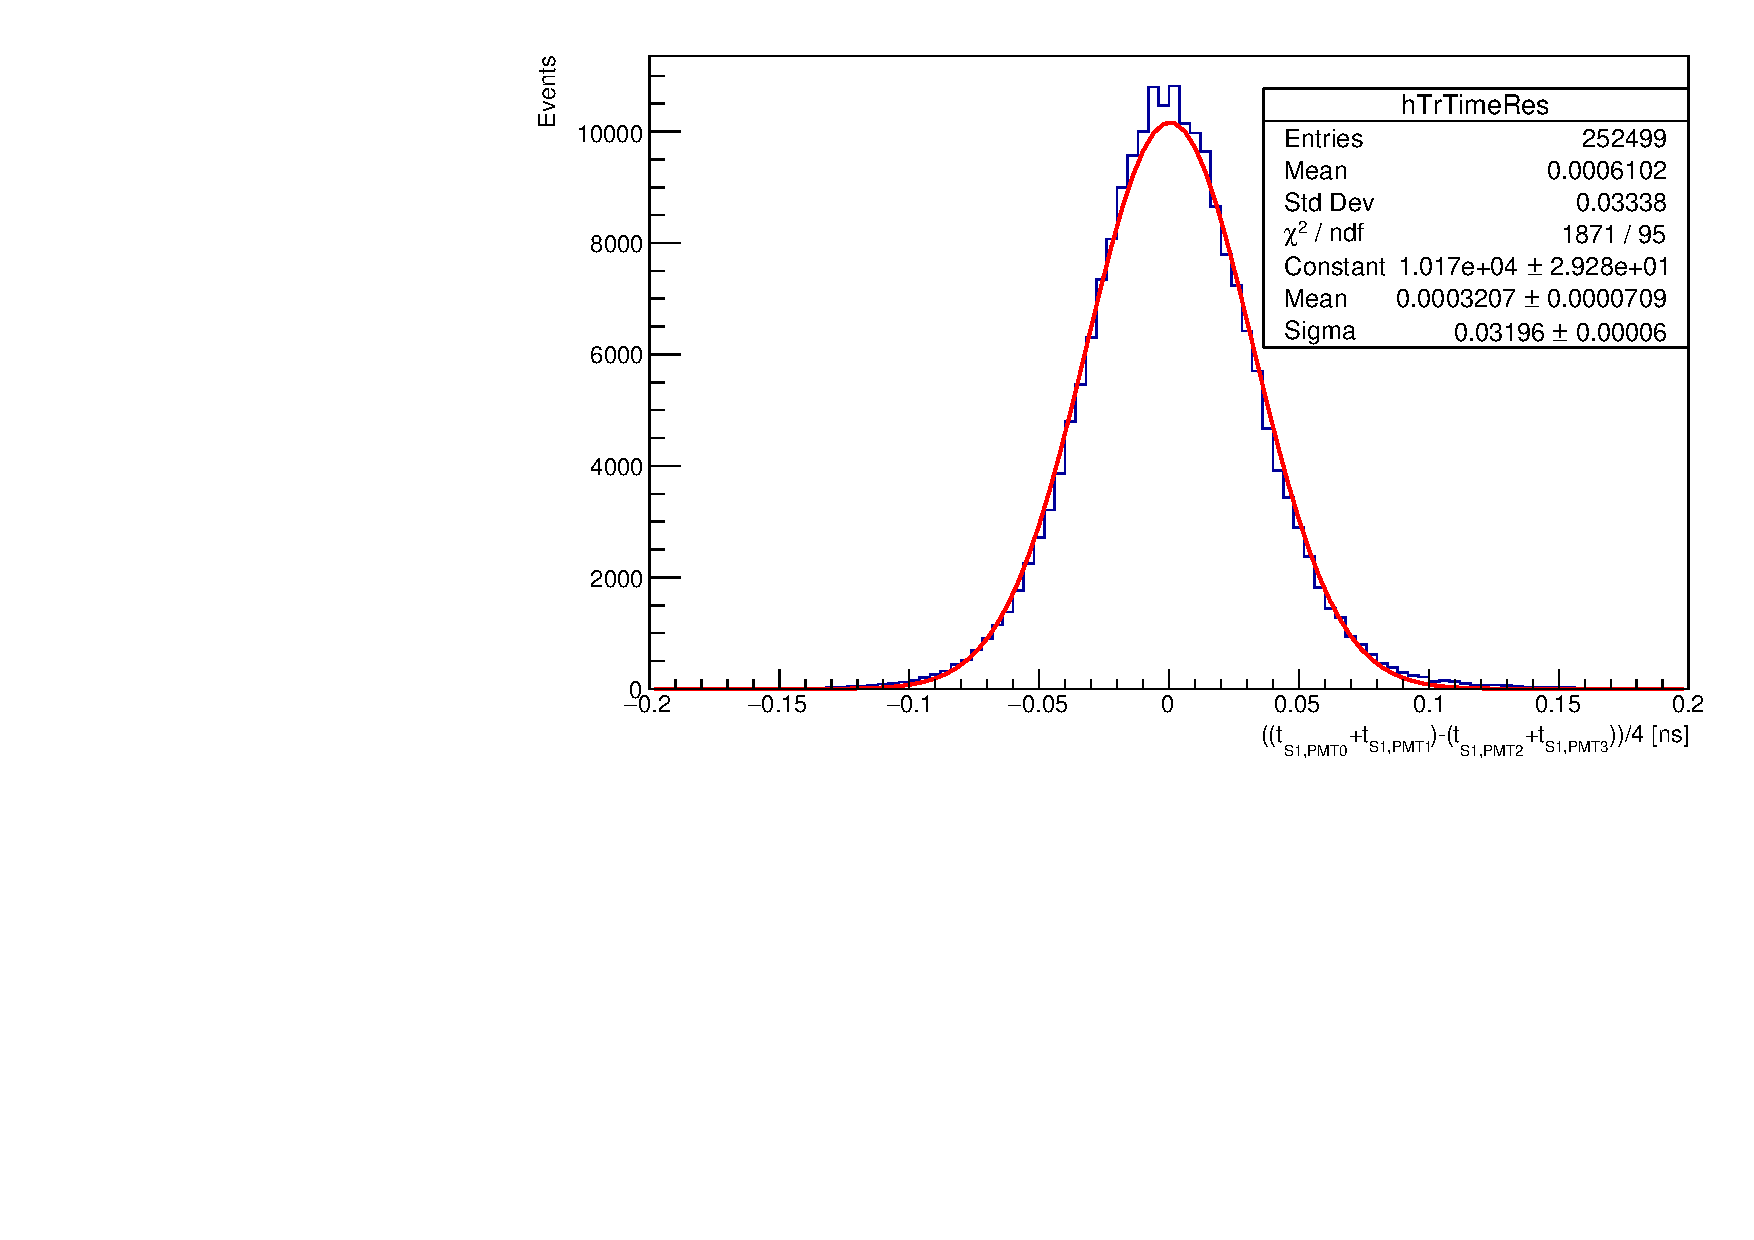
\includegraphics[width=0.65\linewidth]{files/Figures/TrTimeRes.pdf}
  \caption{An example of the timing distribution of $\mathit{S1}$ hits. The time is calculated as an average of the hit time as measured in each of the 4 PMTs.}
  \label{fig:s3Res}
\end{figure}

The $\mathit{S2}$ counter is a scintillator tile of size $120\times120\times5$~mm$^3$, coupled to a 2" PMT R1309, which  2'' PMT R13089 which was connected to the scintillator via long light-guide as shown in Figure~\ref{fig:modblocks}.
The $\mathit{S2}$ counter was placed $(1.4194 \pm 0.0014)~\text{m}$ downstream of $\mathit{S1}$.
The transverse position of $\mathit{S2}$ was adjusted to account for the beam divergence in the moderator blocks.

The analog signals from one of the $\mathit{S1}$ PMTs and $\mathit{S2}$ PMT were fed into NIM discriminator units with a threshold of 30~mV.
Subsequently, the discriminated signals were fed into a NIM coincidence unit, and the coincidence of the two signals was recorded by the DAQ systems of the downstream ToF wall ($\mathit{S4}$).
This information was further used for the time-of-flight analysis of the downstream ToF.

\subsection{Upstream Time of Flight instrumentation $\mathit(S3)$}
\label{subsec:s3Exp}
The $\mathit{S3}$ `upstream' ToF constituent was placed $(1.3225 \pm 0.0014)~\text{m}$ upstream of the upstream side of the HPTPC drift volume in the beamline.
A schematic drawing of the $\mathit{S3}$ ToF wall is shown in Figure~\ref{fig:S3sketch}.
The detector is composed of 22 staggered scintillator bars:  20 bars with dimensions $1.7 \times 6.0 \times 1.0$~cm$^3$ and 2 bars of  $1.5 \times 6.0 \times 1.0$~cm$^3$ placed on top and bottom~\cite{S3-proceedings}.
The overlap between bars was set to 5~mm, thus the active area of the detector was $2.0214~\text{cm}^{2}$.

\begin{figure}
  \centering
  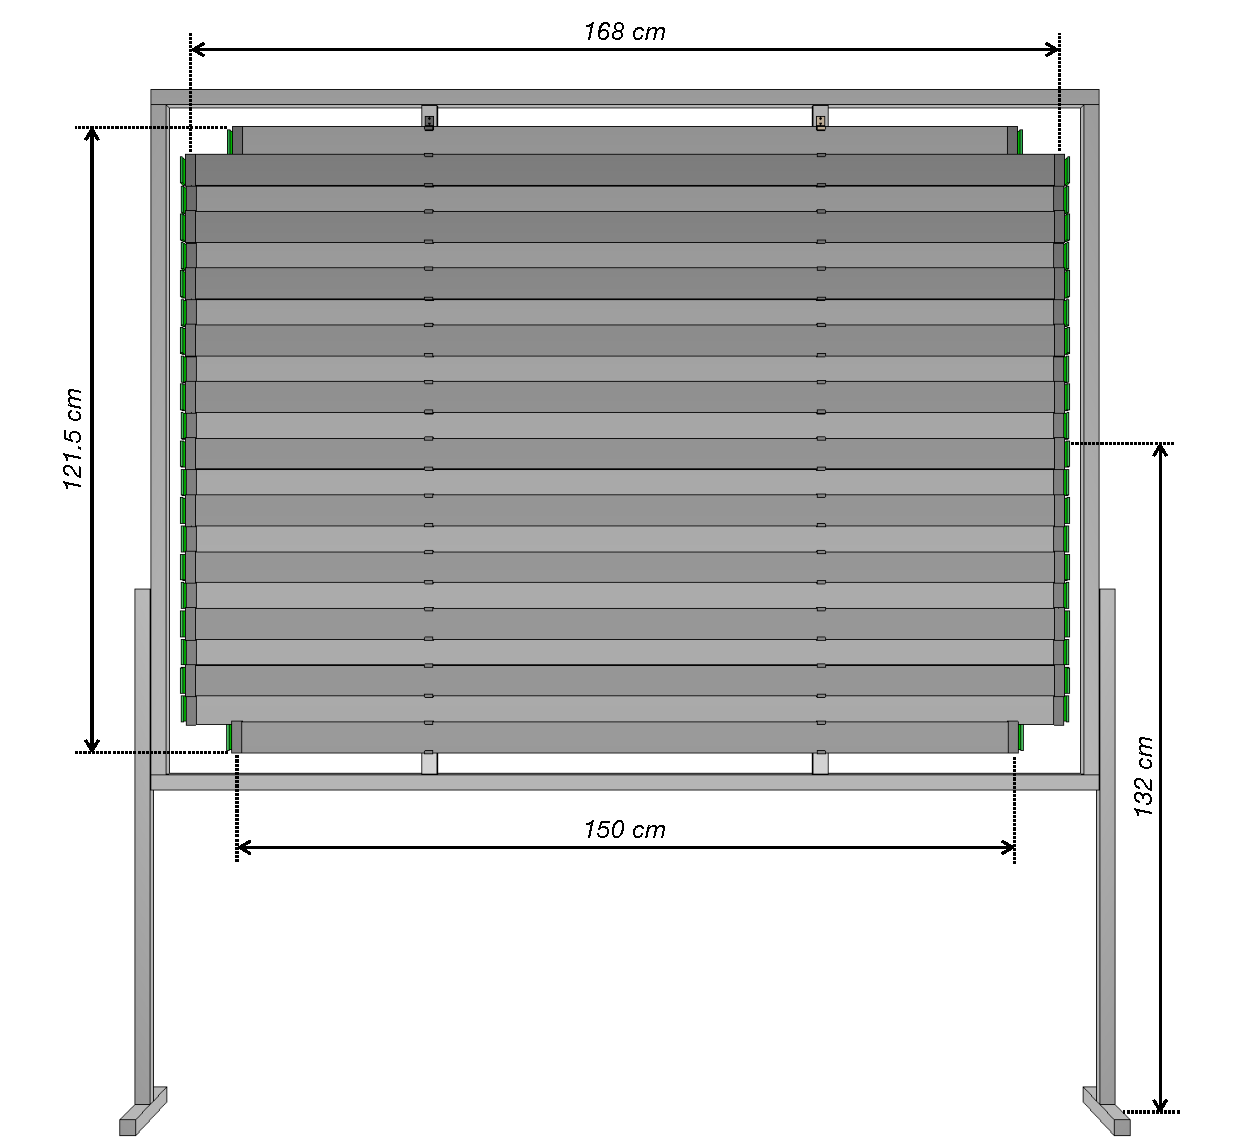
\includegraphics[width=0.54\linewidth]{files/Figures/uToF_sketch.pdf}
  \hfill
  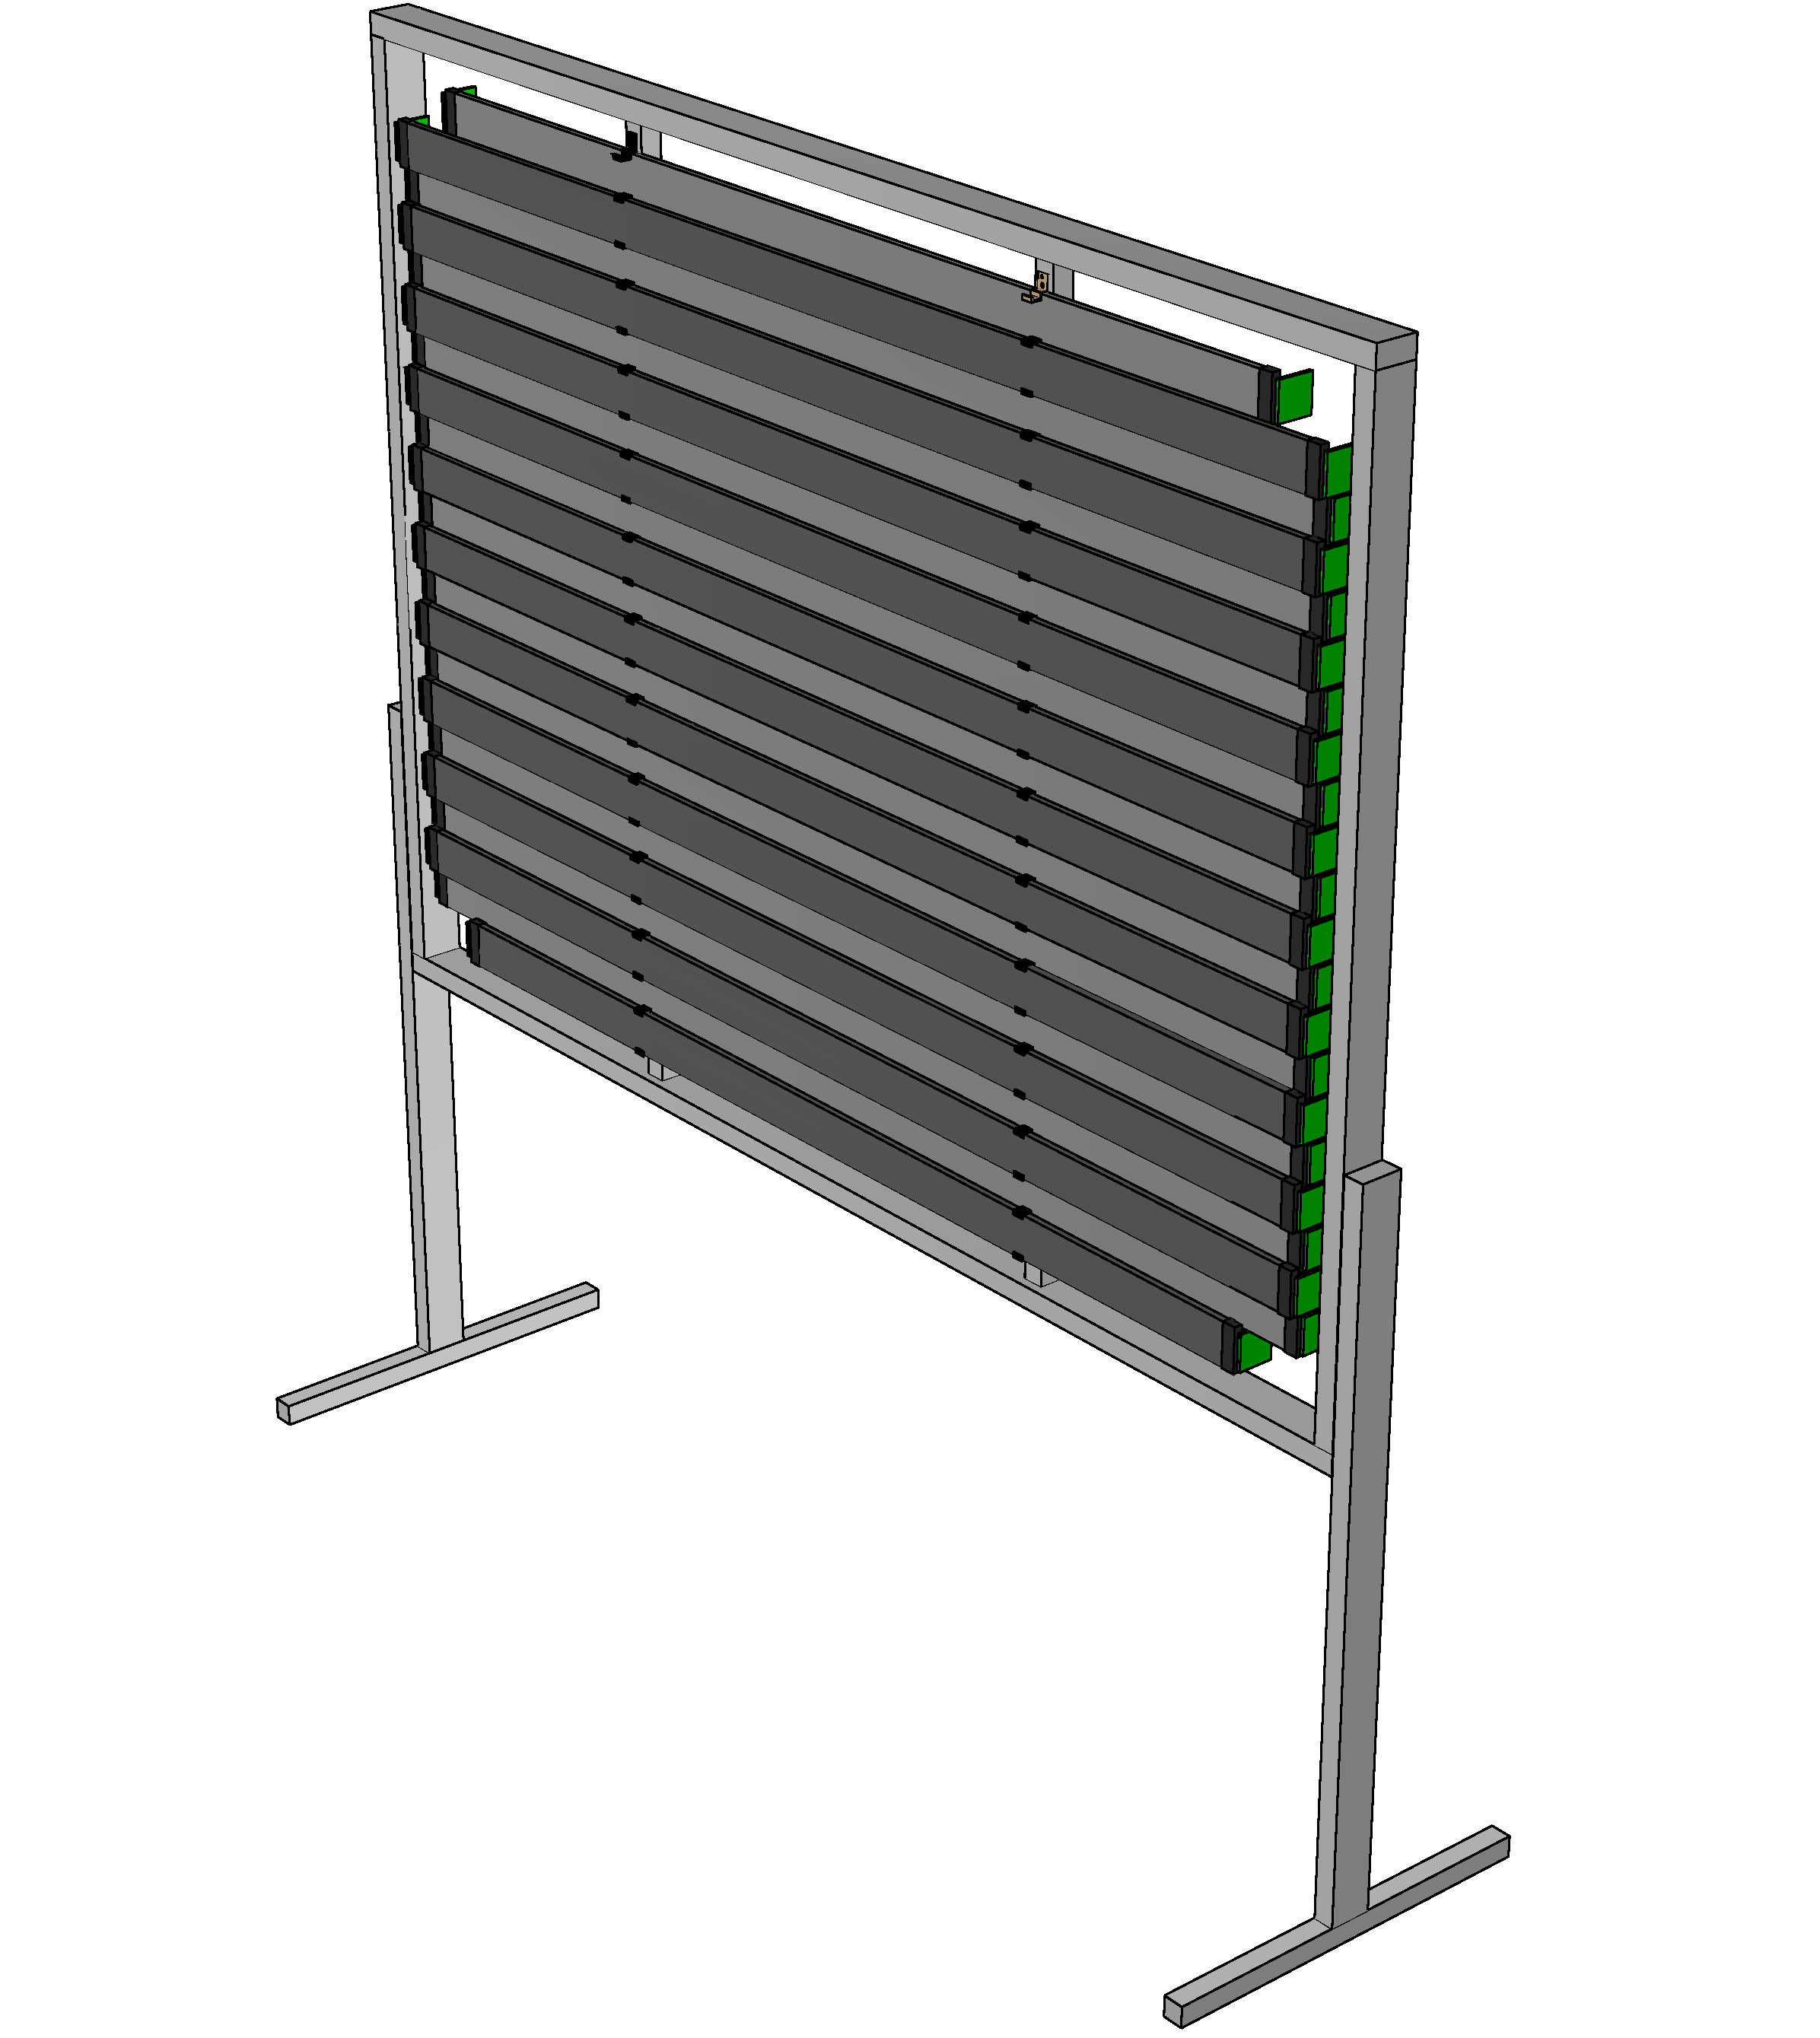
\includegraphics[width=0.43\linewidth]{files/Figures/uTOF_rot.pdf}
  \caption{Sketch of the $\mathit{S3}$ wall \cite{S3-proceedings}.
  Front (left) and rotated (right) views are presented.}
  \label{fig:S3sketch}
\end{figure}

The bars are made from the plastic scintillator, EJ-200 \cite{SCIONIX}, which provides a brightness of 10,000~photons/MeV~deposited.
It also has a suitable optical attenuation length of 4~m and fast timing, with a rise time of 0.9~ns and decay time constant of 2.1~ns.
The scintillation emission spectrum of EJ-200 resides peaks in the violet region of the visible spectrum (435~nm)~\cite{EJ200}, which corresponds well to the photon detection efficiency wavelength range of photosensors used for the readout.
The bars wrapped with an aluminium foil to maximize the light collected.
The foil used had a reflectivity of approximately 60\%.

Arrays of eight $6 \times 6$~mm$^2$ area silicon photomultipliers (SiPMs) S13360-6050PE from Hamamatsu Photonics \cite{Hamamatsu} were coupled to each end of the bar to collect scintillation photons.
The anode signals of the SiPMs are read out, summed and shaped by a dedicated circuit as described in Ref.\,\cite{S3-readout}.
%an 8-channel SiPM anode readout integrated circuit MUSIC-R1. %The construction of the prototype was a joint effort between groups of Geneva and Zurich universities as a part of R\&D for the Timing detector of the SHIP experiment \cite{AK}.

A 64-ch SAMPIC  module was used for the data acquisition.
A SAMPIC chip is a Waveform and Time to Digital Converter (WTDC) 16-channel ASIC which provides a raw time with an ultrafast analog memory allowing fine timing extraction as well as other parameters of the pulse~\cite{SAMPIC}.
Each channel contains a discriminator that can trigger itself independently or participate in a more complex combined trigger. 
Three module ASICs ($16\times3=48$ channels) were connected to the 44 channels of $\mathit{S3}$ and were operated in self-triggering mode.

The trigger conditions are as follows. At least three out of the four $\mathit{S1}$ PMTs must have a signal above a 30~mV threshold.
Additionally, there must be at least one signal in $\mathit{S3}$ above 30~mV.
These $\mathit{S1}$ and $\mathit{S3}$ signals must be coincident within a gate of 70~ns.

A 4th ASIC was used to acquire data from $\mathit{S1}$, the coincidence signal $\mathit{S1} \cap \mathit{S2}$, and the start-of-spill signal from PS.
A second level trigger was implemented in firmware and run on the level of the ASICs: the data were only sent to the hard disk of the DAQ notebook in the case of coincidence between $\mathit{S1}$ channels and channels of three ASICs used for $\mathit{S3}$.

A mean time of light signals detected at two ends of a single bar provides a time reference with a resolution of about 100~ps, while the difference between the time of the light signals gives the position of the interaction along the bar, with a resolution of 1.6~cm.

Examples of reconstructed $XY$ distributions are shown in Figures~\ref{fig:s3XY_pion} and~\ref{fig:s3XY_proton}.
The axes of the distributions shown in Figures~\ref{fig:s3XY_pion} and~\ref{fig:s3XY_proton} are local coordinates for $\mathit{S3}$ where $y=0~\text{cm}$ is the bottom of the active area and $y=120~\text{cm}$ is the top of the active area.
In the $x$ direction, 0~cm is the left-hand side of $\mathit{S3}$ as viewed from $\mathit{S1}$, while $x = 170~\text{cm}$ is the right-hand edge of $\mathit{S3}$.
Figure~\ref{fig:s3XY_pion} shows the spatial distribution of hits in $\mathit{S3}$ thought to be produced by MIPs when no moderator was present in the beamline.
This distribution shows that most of the hits are concentrated in one small spot of the detector (the beam centre).

Figure~\ref{fig:s3XY_proton} shows the spatial distribution of hits identified in $\mathit{S3}$ as protons when 4 moderator blocks were in the beamline.
In contrast to Figure~\ref{fig:s3XY_pion}, the pattern of hits is far more diffuse.
This clearly shows the scattering effect of the moderator blocks.

\todo[inline]{JOCELYN: "to understand whether the axes make sense, the reader needs to know the coordinate system.  The paper needs a paragraph on the coordinates of the upstream TOF somewhere before reconstruction is discussed to make sense of this.  That paragraph should spell out where the TOF is, and where the beam is expected to be, and then the discussion of these figures (that needs to be included in the reconstruction section) should compare the measured beam center position (which can't really be determined from these figures, so the caption should give it, as well as the text), with the expected beam center position."}

\begin{figure}[t]
  \begin{minipage}[t]{0.49\textwidth}
    \centering
    \begin{adjustbox}{max totalsize={\textwidth}{.5\textheight},center}
      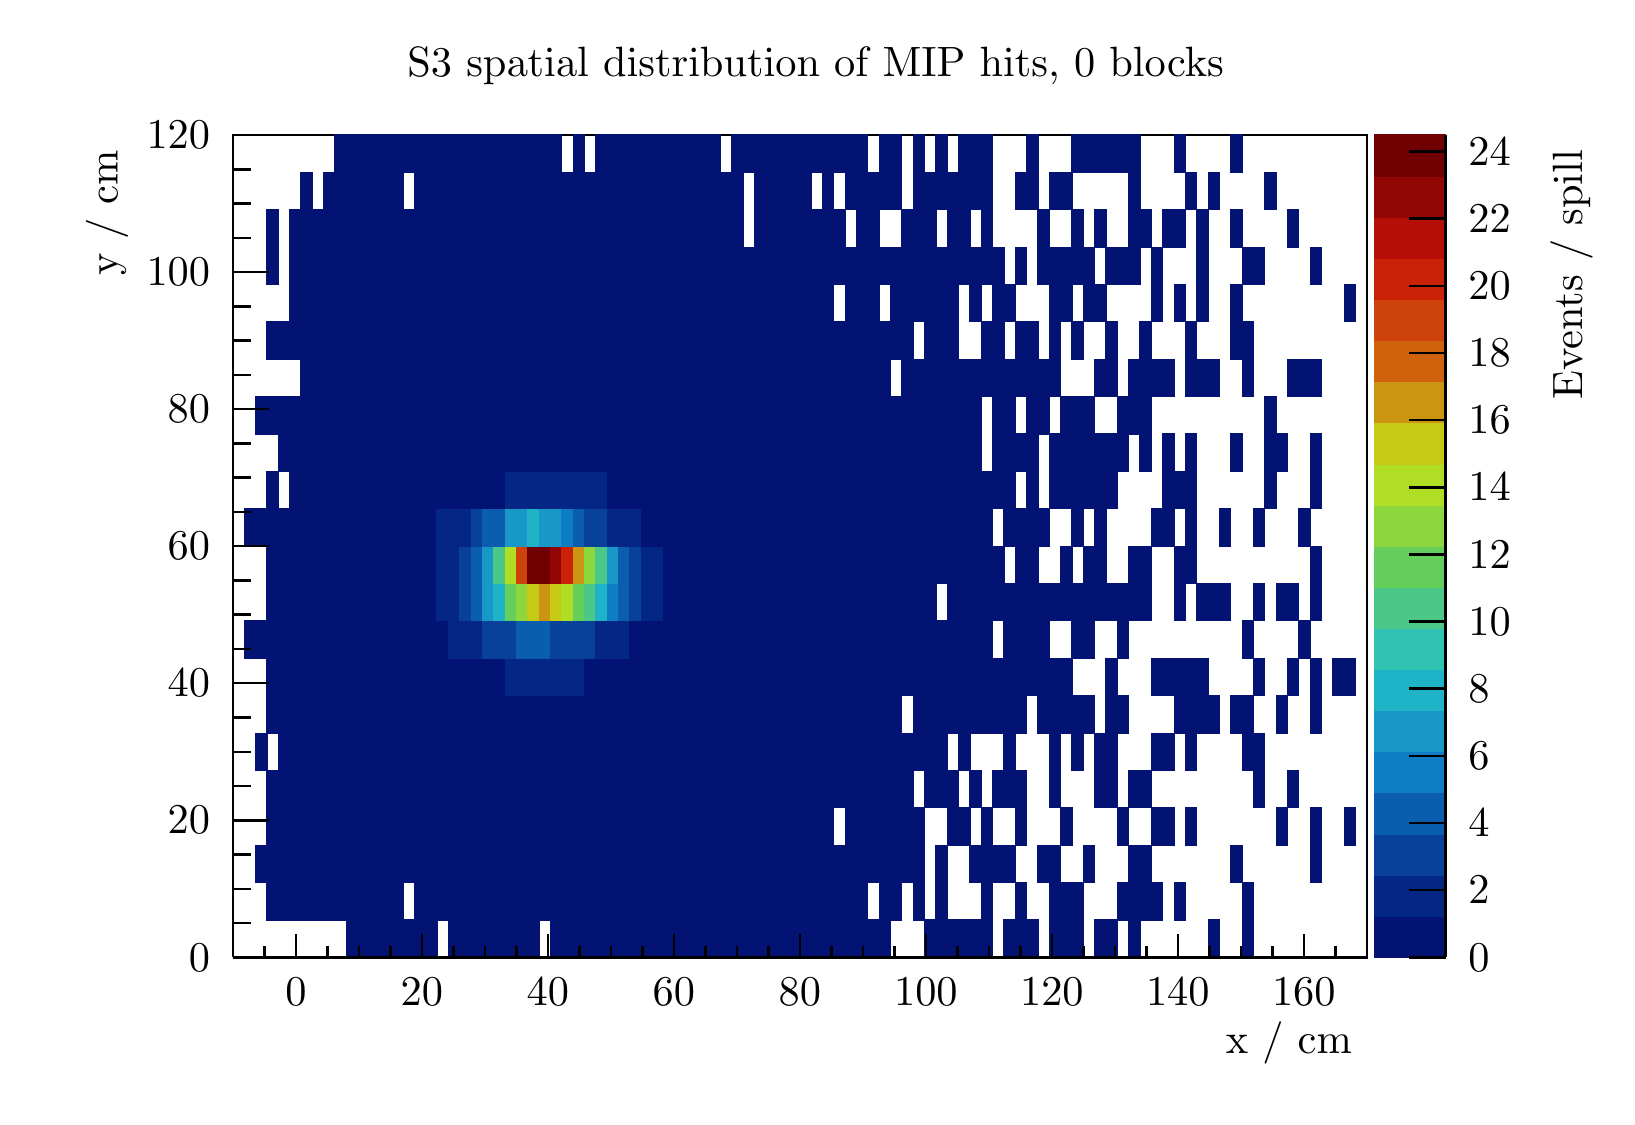
\begin{tikzpicture}
\pgfdeclareplotmark{cross} {
\pgfpathmoveto{\pgfpoint{-0.3\pgfplotmarksize}{\pgfplotmarksize}}
\pgfpathlineto{\pgfpoint{+0.3\pgfplotmarksize}{\pgfplotmarksize}}
\pgfpathlineto{\pgfpoint{+0.3\pgfplotmarksize}{0.3\pgfplotmarksize}}
\pgfpathlineto{\pgfpoint{+1\pgfplotmarksize}{0.3\pgfplotmarksize}}
\pgfpathlineto{\pgfpoint{+1\pgfplotmarksize}{-0.3\pgfplotmarksize}}
\pgfpathlineto{\pgfpoint{+0.3\pgfplotmarksize}{-0.3\pgfplotmarksize}}
\pgfpathlineto{\pgfpoint{+0.3\pgfplotmarksize}{-1.\pgfplotmarksize}}
\pgfpathlineto{\pgfpoint{-0.3\pgfplotmarksize}{-1.\pgfplotmarksize}}
\pgfpathlineto{\pgfpoint{-0.3\pgfplotmarksize}{-0.3\pgfplotmarksize}}
\pgfpathlineto{\pgfpoint{-1.\pgfplotmarksize}{-0.3\pgfplotmarksize}}
\pgfpathlineto{\pgfpoint{-1.\pgfplotmarksize}{0.3\pgfplotmarksize}}
\pgfpathlineto{\pgfpoint{-0.3\pgfplotmarksize}{0.3\pgfplotmarksize}}
\pgfpathclose
\pgfusepathqstroke
}
\pgfdeclareplotmark{cross*} {
\pgfpathmoveto{\pgfpoint{-0.3\pgfplotmarksize}{\pgfplotmarksize}}
\pgfpathlineto{\pgfpoint{+0.3\pgfplotmarksize}{\pgfplotmarksize}}
\pgfpathlineto{\pgfpoint{+0.3\pgfplotmarksize}{0.3\pgfplotmarksize}}
\pgfpathlineto{\pgfpoint{+1\pgfplotmarksize}{0.3\pgfplotmarksize}}
\pgfpathlineto{\pgfpoint{+1\pgfplotmarksize}{-0.3\pgfplotmarksize}}
\pgfpathlineto{\pgfpoint{+0.3\pgfplotmarksize}{-0.3\pgfplotmarksize}}
\pgfpathlineto{\pgfpoint{+0.3\pgfplotmarksize}{-1.\pgfplotmarksize}}
\pgfpathlineto{\pgfpoint{-0.3\pgfplotmarksize}{-1.\pgfplotmarksize}}
\pgfpathlineto{\pgfpoint{-0.3\pgfplotmarksize}{-0.3\pgfplotmarksize}}
\pgfpathlineto{\pgfpoint{-1.\pgfplotmarksize}{-0.3\pgfplotmarksize}}
\pgfpathlineto{\pgfpoint{-1.\pgfplotmarksize}{0.3\pgfplotmarksize}}
\pgfpathlineto{\pgfpoint{-0.3\pgfplotmarksize}{0.3\pgfplotmarksize}}
\pgfpathclose
\pgfusepathqfillstroke
}
\pgfdeclareplotmark{newstar} {
\pgfpathmoveto{\pgfqpoint{0pt}{\pgfplotmarksize}}
\pgfpathlineto{\pgfqpointpolar{44}{0.5\pgfplotmarksize}}
\pgfpathlineto{\pgfqpointpolar{18}{\pgfplotmarksize}}
\pgfpathlineto{\pgfqpointpolar{-20}{0.5\pgfplotmarksize}}
\pgfpathlineto{\pgfqpointpolar{-54}{\pgfplotmarksize}}
\pgfpathlineto{\pgfqpointpolar{-90}{0.5\pgfplotmarksize}}
\pgfpathlineto{\pgfqpointpolar{234}{\pgfplotmarksize}}
\pgfpathlineto{\pgfqpointpolar{198}{0.5\pgfplotmarksize}}
\pgfpathlineto{\pgfqpointpolar{162}{\pgfplotmarksize}}
\pgfpathlineto{\pgfqpointpolar{134}{0.5\pgfplotmarksize}}
\pgfpathclose
\pgfusepathqstroke
}
\pgfdeclareplotmark{newstar*} {
\pgfpathmoveto{\pgfqpoint{0pt}{\pgfplotmarksize}}
\pgfpathlineto{\pgfqpointpolar{44}{0.5\pgfplotmarksize}}
\pgfpathlineto{\pgfqpointpolar{18}{\pgfplotmarksize}}
\pgfpathlineto{\pgfqpointpolar{-20}{0.5\pgfplotmarksize}}
\pgfpathlineto{\pgfqpointpolar{-54}{\pgfplotmarksize}}
\pgfpathlineto{\pgfqpointpolar{-90}{0.5\pgfplotmarksize}}
\pgfpathlineto{\pgfqpointpolar{234}{\pgfplotmarksize}}
\pgfpathlineto{\pgfqpointpolar{198}{0.5\pgfplotmarksize}}
\pgfpathlineto{\pgfqpointpolar{162}{\pgfplotmarksize}}
\pgfpathlineto{\pgfqpointpolar{134}{0.5\pgfplotmarksize}}
\pgfpathclose
\pgfusepathqfillstroke
}
\definecolor{c}{rgb}{1,1,1};
\draw [color=c, fill=c] (0,0) rectangle (20,13.5632);
\draw [color=c, fill=c] (2.6,1.76322) rectangle (17,12.2069);
\definecolor{c}{rgb}{0,0,0};
\draw [c,line width=0.9] (2.6,1.76322) -- (2.6,12.2069) -- (17,12.2069) -- (17,1.76322) -- (2.6,1.76322);
\definecolor{c}{rgb}{1,1,1};
\draw [color=c, fill=c] (2.6,1.76322) rectangle (17,12.2069);
\definecolor{c}{rgb}{0,0,0};
\draw [c,line width=0.9] (2.6,1.76322) -- (2.6,12.2069) -- (17,12.2069) -- (17,1.76322) -- (2.6,1.76322);
\definecolor{c}{rgb}{0.00759013,0.0728653,0.45351};
\draw [color=c, fill=c] (4.04,1.76322) rectangle (4.184,2.23793);
\draw [color=c, fill=c] (4.184,1.76322) rectangle (4.328,2.23793);
\draw [color=c, fill=c] (4.328,1.76322) rectangle (4.472,2.23793);
\draw [color=c, fill=c] (4.472,1.76322) rectangle (4.616,2.23793);
\draw [color=c, fill=c] (4.616,1.76322) rectangle (4.76,2.23793);
\draw [color=c, fill=c] (4.76,1.76322) rectangle (4.904,2.23793);
\draw [color=c, fill=c] (4.904,1.76322) rectangle (5.048,2.23793);
\draw [color=c, fill=c] (5.048,1.76322) rectangle (5.192,2.23793);
\draw [color=c, fill=c] (5.336,1.76322) rectangle (5.48,2.23793);
\draw [color=c, fill=c] (5.48,1.76322) rectangle (5.624,2.23793);
\draw [color=c, fill=c] (5.624,1.76322) rectangle (5.768,2.23793);
\draw [color=c, fill=c] (5.768,1.76322) rectangle (5.912,2.23793);
\draw [color=c, fill=c] (5.912,1.76322) rectangle (6.056,2.23793);
\draw [color=c, fill=c] (6.056,1.76322) rectangle (6.2,2.23793);
\draw [color=c, fill=c] (6.2,1.76322) rectangle (6.344,2.23793);
\draw [color=c, fill=c] (6.344,1.76322) rectangle (6.488,2.23793);
\draw [color=c, fill=c] (6.632,1.76322) rectangle (6.776,2.23793);
\draw [color=c, fill=c] (6.776,1.76322) rectangle (6.92,2.23793);
\draw [color=c, fill=c] (6.92,1.76322) rectangle (7.064,2.23793);
\draw [color=c, fill=c] (7.064,1.76322) rectangle (7.208,2.23793);
\draw [color=c, fill=c] (7.208,1.76322) rectangle (7.352,2.23793);
\draw [color=c, fill=c] (7.352,1.76322) rectangle (7.496,2.23793);
\draw [color=c, fill=c] (7.496,1.76322) rectangle (7.64,2.23793);
\draw [color=c, fill=c] (7.64,1.76322) rectangle (7.784,2.23793);
\draw [color=c, fill=c] (7.784,1.76322) rectangle (7.928,2.23793);
\draw [color=c, fill=c] (7.928,1.76322) rectangle (8.072,2.23793);
\draw [color=c, fill=c] (8.072,1.76322) rectangle (8.216,2.23793);
\draw [color=c, fill=c] (8.216,1.76322) rectangle (8.36,2.23793);
\draw [color=c, fill=c] (8.36,1.76322) rectangle (8.504,2.23793);
\draw [color=c, fill=c] (8.504,1.76322) rectangle (8.648,2.23793);
\draw [color=c, fill=c] (8.648,1.76322) rectangle (8.792,2.23793);
\draw [color=c, fill=c] (8.792,1.76322) rectangle (8.936,2.23793);
\draw [color=c, fill=c] (8.936,1.76322) rectangle (9.08,2.23793);
\draw [color=c, fill=c] (9.08,1.76322) rectangle (9.224,2.23793);
\draw [color=c, fill=c] (9.224,1.76322) rectangle (9.368,2.23793);
\draw [color=c, fill=c] (9.368,1.76322) rectangle (9.512,2.23793);
\draw [color=c, fill=c] (9.512,1.76322) rectangle (9.656,2.23793);
\draw [color=c, fill=c] (9.656,1.76322) rectangle (9.8,2.23793);
\draw [color=c, fill=c] (9.8,1.76322) rectangle (9.944,2.23793);
\draw [color=c, fill=c] (9.944,1.76322) rectangle (10.088,2.23793);
\draw [color=c, fill=c] (10.088,1.76322) rectangle (10.232,2.23793);
\draw [color=c, fill=c] (10.232,1.76322) rectangle (10.376,2.23793);
\draw [color=c, fill=c] (10.376,1.76322) rectangle (10.52,2.23793);
\draw [color=c, fill=c] (10.52,1.76322) rectangle (10.664,2.23793);
\draw [color=c, fill=c] (10.664,1.76322) rectangle (10.808,2.23793);
\draw [color=c, fill=c] (10.808,1.76322) rectangle (10.952,2.23793);
\draw [color=c, fill=c] (11.384,1.76322) rectangle (11.528,2.23793);
\draw [color=c, fill=c] (11.528,1.76322) rectangle (11.672,2.23793);
\draw [color=c, fill=c] (11.672,1.76322) rectangle (11.816,2.23793);
\draw [color=c, fill=c] (11.816,1.76322) rectangle (11.96,2.23793);
\draw [color=c, fill=c] (11.96,1.76322) rectangle (12.104,2.23793);
\draw [color=c, fill=c] (12.104,1.76322) rectangle (12.248,2.23793);
\draw [color=c, fill=c] (12.392,1.76322) rectangle (12.536,2.23793);
\draw [color=c, fill=c] (12.536,1.76322) rectangle (12.68,2.23793);
\draw [color=c, fill=c] (12.68,1.76322) rectangle (12.824,2.23793);
\draw [color=c, fill=c] (12.968,1.76322) rectangle (13.112,2.23793);
\draw [color=c, fill=c] (13.112,1.76322) rectangle (13.256,2.23793);
\draw [color=c, fill=c] (13.256,1.76322) rectangle (13.4,2.23793);
\draw [color=c, fill=c] (13.544,1.76322) rectangle (13.688,2.23793);
\draw [color=c, fill=c] (13.688,1.76322) rectangle (13.832,2.23793);
\draw [color=c, fill=c] (13.976,1.76322) rectangle (14.12,2.23793);
\draw [color=c, fill=c] (14.984,1.76322) rectangle (15.128,2.23793);
\draw [color=c, fill=c] (15.416,1.76322) rectangle (15.56,2.23793);
\draw [color=c, fill=c] (3.032,2.23793) rectangle (3.176,2.71264);
\draw [color=c, fill=c] (3.176,2.23793) rectangle (3.32,2.71264);
\draw [color=c, fill=c] (3.32,2.23793) rectangle (3.464,2.71264);
\draw [color=c, fill=c] (3.464,2.23793) rectangle (3.608,2.71264);
\draw [color=c, fill=c] (3.608,2.23793) rectangle (3.752,2.71264);
\draw [color=c, fill=c] (3.752,2.23793) rectangle (3.896,2.71264);
\draw [color=c, fill=c] (3.896,2.23793) rectangle (4.04,2.71264);
\draw [color=c, fill=c] (4.04,2.23793) rectangle (4.184,2.71264);
\draw [color=c, fill=c] (4.184,2.23793) rectangle (4.328,2.71264);
\draw [color=c, fill=c] (4.328,2.23793) rectangle (4.472,2.71264);
\draw [color=c, fill=c] (4.472,2.23793) rectangle (4.616,2.71264);
\draw [color=c, fill=c] (4.616,2.23793) rectangle (4.76,2.71264);
\draw [color=c, fill=c] (4.904,2.23793) rectangle (5.048,2.71264);
\draw [color=c, fill=c] (5.048,2.23793) rectangle (5.192,2.71264);
\draw [color=c, fill=c] (5.192,2.23793) rectangle (5.336,2.71264);
\draw [color=c, fill=c] (5.336,2.23793) rectangle (5.48,2.71264);
\draw [color=c, fill=c] (5.48,2.23793) rectangle (5.624,2.71264);
\draw [color=c, fill=c] (5.624,2.23793) rectangle (5.768,2.71264);
\draw [color=c, fill=c] (5.768,2.23793) rectangle (5.912,2.71264);
\draw [color=c, fill=c] (5.912,2.23793) rectangle (6.056,2.71264);
\draw [color=c, fill=c] (6.056,2.23793) rectangle (6.2,2.71264);
\draw [color=c, fill=c] (6.2,2.23793) rectangle (6.344,2.71264);
\draw [color=c, fill=c] (6.344,2.23793) rectangle (6.488,2.71264);
\draw [color=c, fill=c] (6.488,2.23793) rectangle (6.632,2.71264);
\draw [color=c, fill=c] (6.632,2.23793) rectangle (6.776,2.71264);
\draw [color=c, fill=c] (6.776,2.23793) rectangle (6.92,2.71264);
\draw [color=c, fill=c] (6.92,2.23793) rectangle (7.064,2.71264);
\draw [color=c, fill=c] (7.064,2.23793) rectangle (7.208,2.71264);
\draw [color=c, fill=c] (7.208,2.23793) rectangle (7.352,2.71264);
\draw [color=c, fill=c] (7.352,2.23793) rectangle (7.496,2.71264);
\draw [color=c, fill=c] (7.496,2.23793) rectangle (7.64,2.71264);
\draw [color=c, fill=c] (7.64,2.23793) rectangle (7.784,2.71264);
\draw [color=c, fill=c] (7.784,2.23793) rectangle (7.928,2.71264);
\draw [color=c, fill=c] (7.928,2.23793) rectangle (8.072,2.71264);
\draw [color=c, fill=c] (8.072,2.23793) rectangle (8.216,2.71264);
\draw [color=c, fill=c] (8.216,2.23793) rectangle (8.36,2.71264);
\draw [color=c, fill=c] (8.36,2.23793) rectangle (8.504,2.71264);
\draw [color=c, fill=c] (8.504,2.23793) rectangle (8.648,2.71264);
\draw [color=c, fill=c] (8.648,2.23793) rectangle (8.792,2.71264);
\draw [color=c, fill=c] (8.792,2.23793) rectangle (8.936,2.71264);
\draw [color=c, fill=c] (8.936,2.23793) rectangle (9.08,2.71264);
\draw [color=c, fill=c] (9.08,2.23793) rectangle (9.224,2.71264);
\draw [color=c, fill=c] (9.224,2.23793) rectangle (9.368,2.71264);
\draw [color=c, fill=c] (9.368,2.23793) rectangle (9.512,2.71264);
\draw [color=c, fill=c] (9.512,2.23793) rectangle (9.656,2.71264);
\draw [color=c, fill=c] (9.656,2.23793) rectangle (9.8,2.71264);
\draw [color=c, fill=c] (9.8,2.23793) rectangle (9.944,2.71264);
\draw [color=c, fill=c] (9.944,2.23793) rectangle (10.088,2.71264);
\draw [color=c, fill=c] (10.088,2.23793) rectangle (10.232,2.71264);
\draw [color=c, fill=c] (10.232,2.23793) rectangle (10.376,2.71264);
\draw [color=c, fill=c] (10.376,2.23793) rectangle (10.52,2.71264);
\draw [color=c, fill=c] (10.52,2.23793) rectangle (10.664,2.71264);
\draw [color=c, fill=c] (10.808,2.23793) rectangle (10.952,2.71264);
\draw [color=c, fill=c] (10.952,2.23793) rectangle (11.096,2.71264);
\draw [color=c, fill=c] (11.24,2.23793) rectangle (11.384,2.71264);
\draw [color=c, fill=c] (11.528,2.23793) rectangle (11.672,2.71264);
\draw [color=c, fill=c] (12.104,2.23793) rectangle (12.248,2.71264);
\draw [color=c, fill=c] (12.536,2.23793) rectangle (12.68,2.71264);
\draw [color=c, fill=c] (12.968,2.23793) rectangle (13.112,2.71264);
\draw [color=c, fill=c] (13.112,2.23793) rectangle (13.256,2.71264);
\draw [color=c, fill=c] (13.256,2.23793) rectangle (13.4,2.71264);
\draw [color=c, fill=c] (13.832,2.23793) rectangle (13.976,2.71264);
\draw [color=c, fill=c] (13.976,2.23793) rectangle (14.12,2.71264);
\draw [color=c, fill=c] (14.12,2.23793) rectangle (14.264,2.71264);
\draw [color=c, fill=c] (14.264,2.23793) rectangle (14.408,2.71264);
\draw [color=c, fill=c] (14.552,2.23793) rectangle (14.696,2.71264);
\draw [color=c, fill=c] (15.416,2.23793) rectangle (15.56,2.71264);
\draw [color=c, fill=c] (2.888,2.71264) rectangle (3.032,3.18736);
\draw [color=c, fill=c] (3.032,2.71264) rectangle (3.176,3.18736);
\draw [color=c, fill=c] (3.176,2.71264) rectangle (3.32,3.18736);
\draw [color=c, fill=c] (3.32,2.71264) rectangle (3.464,3.18736);
\draw [color=c, fill=c] (3.464,2.71264) rectangle (3.608,3.18736);
\draw [color=c, fill=c] (3.608,2.71264) rectangle (3.752,3.18736);
\draw [color=c, fill=c] (3.752,2.71264) rectangle (3.896,3.18736);
\draw [color=c, fill=c] (3.896,2.71264) rectangle (4.04,3.18736);
\draw [color=c, fill=c] (4.04,2.71264) rectangle (4.184,3.18736);
\draw [color=c, fill=c] (4.184,2.71264) rectangle (4.328,3.18736);
\draw [color=c, fill=c] (4.328,2.71264) rectangle (4.472,3.18736);
\draw [color=c, fill=c] (4.472,2.71264) rectangle (4.616,3.18736);
\draw [color=c, fill=c] (4.616,2.71264) rectangle (4.76,3.18736);
\draw [color=c, fill=c] (4.76,2.71264) rectangle (4.904,3.18736);
\draw [color=c, fill=c] (4.904,2.71264) rectangle (5.048,3.18736);
\draw [color=c, fill=c] (5.048,2.71264) rectangle (5.192,3.18736);
\draw [color=c, fill=c] (5.192,2.71264) rectangle (5.336,3.18736);
\draw [color=c, fill=c] (5.336,2.71264) rectangle (5.48,3.18736);
\draw [color=c, fill=c] (5.48,2.71264) rectangle (5.624,3.18736);
\draw [color=c, fill=c] (5.624,2.71264) rectangle (5.768,3.18736);
\draw [color=c, fill=c] (5.768,2.71264) rectangle (5.912,3.18736);
\draw [color=c, fill=c] (5.912,2.71264) rectangle (6.056,3.18736);
\draw [color=c, fill=c] (6.056,2.71264) rectangle (6.2,3.18736);
\draw [color=c, fill=c] (6.2,2.71264) rectangle (6.344,3.18736);
\draw [color=c, fill=c] (6.344,2.71264) rectangle (6.488,3.18736);
\draw [color=c, fill=c] (6.488,2.71264) rectangle (6.632,3.18736);
\draw [color=c, fill=c] (6.632,2.71264) rectangle (6.776,3.18736);
\draw [color=c, fill=c] (6.776,2.71264) rectangle (6.92,3.18736);
\draw [color=c, fill=c] (6.92,2.71264) rectangle (7.064,3.18736);
\draw [color=c, fill=c] (7.064,2.71264) rectangle (7.208,3.18736);
\draw [color=c, fill=c] (7.208,2.71264) rectangle (7.352,3.18736);
\draw [color=c, fill=c] (7.352,2.71264) rectangle (7.496,3.18736);
\draw [color=c, fill=c] (7.496,2.71264) rectangle (7.64,3.18736);
\draw [color=c, fill=c] (7.64,2.71264) rectangle (7.784,3.18736);
\draw [color=c, fill=c] (7.784,2.71264) rectangle (7.928,3.18736);
\draw [color=c, fill=c] (7.928,2.71264) rectangle (8.072,3.18736);
\draw [color=c, fill=c] (8.072,2.71264) rectangle (8.216,3.18736);
\draw [color=c, fill=c] (8.216,2.71264) rectangle (8.36,3.18736);
\draw [color=c, fill=c] (8.36,2.71264) rectangle (8.504,3.18736);
\draw [color=c, fill=c] (8.504,2.71264) rectangle (8.648,3.18736);
\draw [color=c, fill=c] (8.648,2.71264) rectangle (8.792,3.18736);
\draw [color=c, fill=c] (8.792,2.71264) rectangle (8.936,3.18736);
\draw [color=c, fill=c] (8.936,2.71264) rectangle (9.08,3.18736);
\draw [color=c, fill=c] (9.08,2.71264) rectangle (9.224,3.18736);
\draw [color=c, fill=c] (9.224,2.71264) rectangle (9.368,3.18736);
\draw [color=c, fill=c] (9.368,2.71264) rectangle (9.512,3.18736);
\draw [color=c, fill=c] (9.512,2.71264) rectangle (9.656,3.18736);
\draw [color=c, fill=c] (9.656,2.71264) rectangle (9.8,3.18736);
\draw [color=c, fill=c] (9.8,2.71264) rectangle (9.944,3.18736);
\draw [color=c, fill=c] (9.944,2.71264) rectangle (10.088,3.18736);
\draw [color=c, fill=c] (10.088,2.71264) rectangle (10.232,3.18736);
\draw [color=c, fill=c] (10.232,2.71264) rectangle (10.376,3.18736);
\draw [color=c, fill=c] (10.376,2.71264) rectangle (10.52,3.18736);
\draw [color=c, fill=c] (10.52,2.71264) rectangle (10.664,3.18736);
\draw [color=c, fill=c] (10.664,2.71264) rectangle (10.808,3.18736);
\draw [color=c, fill=c] (10.808,2.71264) rectangle (10.952,3.18736);
\draw [color=c, fill=c] (10.952,2.71264) rectangle (11.096,3.18736);
\draw [color=c, fill=c] (11.096,2.71264) rectangle (11.24,3.18736);
\draw [color=c, fill=c] (11.24,2.71264) rectangle (11.384,3.18736);
\draw [color=c, fill=c] (11.528,2.71264) rectangle (11.672,3.18736);
\draw [color=c, fill=c] (11.96,2.71264) rectangle (12.104,3.18736);
\draw [color=c, fill=c] (12.104,2.71264) rectangle (12.248,3.18736);
\draw [color=c, fill=c] (12.248,2.71264) rectangle (12.392,3.18736);
\draw [color=c, fill=c] (12.392,2.71264) rectangle (12.536,3.18736);
\draw [color=c, fill=c] (12.824,2.71264) rectangle (12.968,3.18736);
\draw [color=c, fill=c] (12.968,2.71264) rectangle (13.112,3.18736);
\draw [color=c, fill=c] (13.4,2.71264) rectangle (13.544,3.18736);
\draw [color=c, fill=c] (13.976,2.71264) rectangle (14.12,3.18736);
\draw [color=c, fill=c] (14.12,2.71264) rectangle (14.264,3.18736);
\draw [color=c, fill=c] (15.272,2.71264) rectangle (15.416,3.18736);
\draw [color=c, fill=c] (16.28,2.71264) rectangle (16.424,3.18736);
\draw [color=c, fill=c] (3.032,3.18736) rectangle (3.176,3.66207);
\draw [color=c, fill=c] (3.176,3.18736) rectangle (3.32,3.66207);
\draw [color=c, fill=c] (3.32,3.18736) rectangle (3.464,3.66207);
\draw [color=c, fill=c] (3.464,3.18736) rectangle (3.608,3.66207);
\draw [color=c, fill=c] (3.608,3.18736) rectangle (3.752,3.66207);
\draw [color=c, fill=c] (3.752,3.18736) rectangle (3.896,3.66207);
\draw [color=c, fill=c] (3.896,3.18736) rectangle (4.04,3.66207);
\draw [color=c, fill=c] (4.04,3.18736) rectangle (4.184,3.66207);
\draw [color=c, fill=c] (4.184,3.18736) rectangle (4.328,3.66207);
\draw [color=c, fill=c] (4.328,3.18736) rectangle (4.472,3.66207);
\draw [color=c, fill=c] (4.472,3.18736) rectangle (4.616,3.66207);
\draw [color=c, fill=c] (4.616,3.18736) rectangle (4.76,3.66207);
\draw [color=c, fill=c] (4.76,3.18736) rectangle (4.904,3.66207);
\draw [color=c, fill=c] (4.904,3.18736) rectangle (5.048,3.66207);
\draw [color=c, fill=c] (5.048,3.18736) rectangle (5.192,3.66207);
\draw [color=c, fill=c] (5.192,3.18736) rectangle (5.336,3.66207);
\draw [color=c, fill=c] (5.336,3.18736) rectangle (5.48,3.66207);
\draw [color=c, fill=c] (5.48,3.18736) rectangle (5.624,3.66207);
\draw [color=c, fill=c] (5.624,3.18736) rectangle (5.768,3.66207);
\draw [color=c, fill=c] (5.768,3.18736) rectangle (5.912,3.66207);
\draw [color=c, fill=c] (5.912,3.18736) rectangle (6.056,3.66207);
\draw [color=c, fill=c] (6.056,3.18736) rectangle (6.2,3.66207);
\draw [color=c, fill=c] (6.2,3.18736) rectangle (6.344,3.66207);
\draw [color=c, fill=c] (6.344,3.18736) rectangle (6.488,3.66207);
\draw [color=c, fill=c] (6.488,3.18736) rectangle (6.632,3.66207);
\draw [color=c, fill=c] (6.632,3.18736) rectangle (6.776,3.66207);
\draw [color=c, fill=c] (6.776,3.18736) rectangle (6.92,3.66207);
\draw [color=c, fill=c] (6.92,3.18736) rectangle (7.064,3.66207);
\draw [color=c, fill=c] (7.064,3.18736) rectangle (7.208,3.66207);
\draw [color=c, fill=c] (7.208,3.18736) rectangle (7.352,3.66207);
\draw [color=c, fill=c] (7.352,3.18736) rectangle (7.496,3.66207);
\draw [color=c, fill=c] (7.496,3.18736) rectangle (7.64,3.66207);
\draw [color=c, fill=c] (7.64,3.18736) rectangle (7.784,3.66207);
\draw [color=c, fill=c] (7.784,3.18736) rectangle (7.928,3.66207);
\draw [color=c, fill=c] (7.928,3.18736) rectangle (8.072,3.66207);
\draw [color=c, fill=c] (8.072,3.18736) rectangle (8.216,3.66207);
\draw [color=c, fill=c] (8.216,3.18736) rectangle (8.36,3.66207);
\draw [color=c, fill=c] (8.36,3.18736) rectangle (8.504,3.66207);
\draw [color=c, fill=c] (8.504,3.18736) rectangle (8.648,3.66207);
\draw [color=c, fill=c] (8.648,3.18736) rectangle (8.792,3.66207);
\draw [color=c, fill=c] (8.792,3.18736) rectangle (8.936,3.66207);
\draw [color=c, fill=c] (8.936,3.18736) rectangle (9.08,3.66207);
\draw [color=c, fill=c] (9.08,3.18736) rectangle (9.224,3.66207);
\draw [color=c, fill=c] (9.224,3.18736) rectangle (9.368,3.66207);
\draw [color=c, fill=c] (9.368,3.18736) rectangle (9.512,3.66207);
\draw [color=c, fill=c] (9.512,3.18736) rectangle (9.656,3.66207);
\draw [color=c, fill=c] (9.656,3.18736) rectangle (9.8,3.66207);
\draw [color=c, fill=c] (9.8,3.18736) rectangle (9.944,3.66207);
\draw [color=c, fill=c] (9.944,3.18736) rectangle (10.088,3.66207);
\draw [color=c, fill=c] (10.088,3.18736) rectangle (10.232,3.66207);
\draw [color=c, fill=c] (10.376,3.18736) rectangle (10.52,3.66207);
\draw [color=c, fill=c] (10.52,3.18736) rectangle (10.664,3.66207);
\draw [color=c, fill=c] (10.664,3.18736) rectangle (10.808,3.66207);
\draw [color=c, fill=c] (10.808,3.18736) rectangle (10.952,3.66207);
\draw [color=c, fill=c] (10.952,3.18736) rectangle (11.096,3.66207);
\draw [color=c, fill=c] (11.096,3.18736) rectangle (11.24,3.66207);
\draw [color=c, fill=c] (11.24,3.18736) rectangle (11.384,3.66207);
\draw [color=c, fill=c] (11.672,3.18736) rectangle (11.816,3.66207);
\draw [color=c, fill=c] (11.816,3.18736) rectangle (11.96,3.66207);
\draw [color=c, fill=c] (12.104,3.18736) rectangle (12.248,3.66207);
\draw [color=c, fill=c] (12.536,3.18736) rectangle (12.68,3.66207);
\draw [color=c, fill=c] (13.112,3.18736) rectangle (13.256,3.66207);
\draw [color=c, fill=c] (13.832,3.18736) rectangle (13.976,3.66207);
\draw [color=c, fill=c] (14.264,3.18736) rectangle (14.408,3.66207);
\draw [color=c, fill=c] (14.408,3.18736) rectangle (14.552,3.66207);
\draw [color=c, fill=c] (14.696,3.18736) rectangle (14.84,3.66207);
\draw [color=c, fill=c] (15.848,3.18736) rectangle (15.992,3.66207);
\draw [color=c, fill=c] (16.28,3.18736) rectangle (16.424,3.66207);
\draw [color=c, fill=c] (16.712,3.18736) rectangle (16.856,3.66207);
\draw [color=c, fill=c] (3.032,3.66207) rectangle (3.176,4.13678);
\draw [color=c, fill=c] (3.176,3.66207) rectangle (3.32,4.13678);
\draw [color=c, fill=c] (3.32,3.66207) rectangle (3.464,4.13678);
\draw [color=c, fill=c] (3.464,3.66207) rectangle (3.608,4.13678);
\draw [color=c, fill=c] (3.608,3.66207) rectangle (3.752,4.13678);
\draw [color=c, fill=c] (3.752,3.66207) rectangle (3.896,4.13678);
\draw [color=c, fill=c] (3.896,3.66207) rectangle (4.04,4.13678);
\draw [color=c, fill=c] (4.04,3.66207) rectangle (4.184,4.13678);
\draw [color=c, fill=c] (4.184,3.66207) rectangle (4.328,4.13678);
\draw [color=c, fill=c] (4.328,3.66207) rectangle (4.472,4.13678);
\draw [color=c, fill=c] (4.472,3.66207) rectangle (4.616,4.13678);
\draw [color=c, fill=c] (4.616,3.66207) rectangle (4.76,4.13678);
\draw [color=c, fill=c] (4.76,3.66207) rectangle (4.904,4.13678);
\draw [color=c, fill=c] (4.904,3.66207) rectangle (5.048,4.13678);
\draw [color=c, fill=c] (5.048,3.66207) rectangle (5.192,4.13678);
\draw [color=c, fill=c] (5.192,3.66207) rectangle (5.336,4.13678);
\draw [color=c, fill=c] (5.336,3.66207) rectangle (5.48,4.13678);
\draw [color=c, fill=c] (5.48,3.66207) rectangle (5.624,4.13678);
\draw [color=c, fill=c] (5.624,3.66207) rectangle (5.768,4.13678);
\draw [color=c, fill=c] (5.768,3.66207) rectangle (5.912,4.13678);
\draw [color=c, fill=c] (5.912,3.66207) rectangle (6.056,4.13678);
\draw [color=c, fill=c] (6.056,3.66207) rectangle (6.2,4.13678);
\draw [color=c, fill=c] (6.2,3.66207) rectangle (6.344,4.13678);
\draw [color=c, fill=c] (6.344,3.66207) rectangle (6.488,4.13678);
\draw [color=c, fill=c] (6.488,3.66207) rectangle (6.632,4.13678);
\draw [color=c, fill=c] (6.632,3.66207) rectangle (6.776,4.13678);
\draw [color=c, fill=c] (6.776,3.66207) rectangle (6.92,4.13678);
\draw [color=c, fill=c] (6.92,3.66207) rectangle (7.064,4.13678);
\draw [color=c, fill=c] (7.064,3.66207) rectangle (7.208,4.13678);
\draw [color=c, fill=c] (7.208,3.66207) rectangle (7.352,4.13678);
\draw [color=c, fill=c] (7.352,3.66207) rectangle (7.496,4.13678);
\draw [color=c, fill=c] (7.496,3.66207) rectangle (7.64,4.13678);
\draw [color=c, fill=c] (7.64,3.66207) rectangle (7.784,4.13678);
\draw [color=c, fill=c] (7.784,3.66207) rectangle (7.928,4.13678);
\draw [color=c, fill=c] (7.928,3.66207) rectangle (8.072,4.13678);
\draw [color=c, fill=c] (8.072,3.66207) rectangle (8.216,4.13678);
\draw [color=c, fill=c] (8.216,3.66207) rectangle (8.36,4.13678);
\draw [color=c, fill=c] (8.36,3.66207) rectangle (8.504,4.13678);
\draw [color=c, fill=c] (8.504,3.66207) rectangle (8.648,4.13678);
\draw [color=c, fill=c] (8.648,3.66207) rectangle (8.792,4.13678);
\draw [color=c, fill=c] (8.792,3.66207) rectangle (8.936,4.13678);
\draw [color=c, fill=c] (8.936,3.66207) rectangle (9.08,4.13678);
\draw [color=c, fill=c] (9.08,3.66207) rectangle (9.224,4.13678);
\draw [color=c, fill=c] (9.224,3.66207) rectangle (9.368,4.13678);
\draw [color=c, fill=c] (9.368,3.66207) rectangle (9.512,4.13678);
\draw [color=c, fill=c] (9.512,3.66207) rectangle (9.656,4.13678);
\draw [color=c, fill=c] (9.656,3.66207) rectangle (9.8,4.13678);
\draw [color=c, fill=c] (9.8,3.66207) rectangle (9.944,4.13678);
\draw [color=c, fill=c] (9.944,3.66207) rectangle (10.088,4.13678);
\draw [color=c, fill=c] (10.088,3.66207) rectangle (10.232,4.13678);
\draw [color=c, fill=c] (10.232,3.66207) rectangle (10.376,4.13678);
\draw [color=c, fill=c] (10.376,3.66207) rectangle (10.52,4.13678);
\draw [color=c, fill=c] (10.52,3.66207) rectangle (10.664,4.13678);
\draw [color=c, fill=c] (10.664,3.66207) rectangle (10.808,4.13678);
\draw [color=c, fill=c] (10.808,3.66207) rectangle (10.952,4.13678);
\draw [color=c, fill=c] (10.952,3.66207) rectangle (11.096,4.13678);
\draw [color=c, fill=c] (11.096,3.66207) rectangle (11.24,4.13678);
\draw [color=c, fill=c] (11.384,3.66207) rectangle (11.528,4.13678);
\draw [color=c, fill=c] (11.528,3.66207) rectangle (11.672,4.13678);
\draw [color=c, fill=c] (11.672,3.66207) rectangle (11.816,4.13678);
\draw [color=c, fill=c] (11.96,3.66207) rectangle (12.104,4.13678);
\draw [color=c, fill=c] (12.248,3.66207) rectangle (12.392,4.13678);
\draw [color=c, fill=c] (12.392,3.66207) rectangle (12.536,4.13678);
\draw [color=c, fill=c] (12.536,3.66207) rectangle (12.68,4.13678);
\draw [color=c, fill=c] (12.968,3.66207) rectangle (13.112,4.13678);
\draw [color=c, fill=c] (13.544,3.66207) rectangle (13.688,4.13678);
\draw [color=c, fill=c] (13.688,3.66207) rectangle (13.832,4.13678);
\draw [color=c, fill=c] (13.976,3.66207) rectangle (14.12,4.13678);
\draw [color=c, fill=c] (14.12,3.66207) rectangle (14.264,4.13678);
\draw [color=c, fill=c] (15.56,3.66207) rectangle (15.704,4.13678);
\draw [color=c, fill=c] (15.992,3.66207) rectangle (16.136,4.13678);
\draw [color=c, fill=c] (2.888,4.13678) rectangle (3.032,4.61149);
\draw [color=c, fill=c] (3.176,4.13678) rectangle (3.32,4.61149);
\draw [color=c, fill=c] (3.32,4.13678) rectangle (3.464,4.61149);
\draw [color=c, fill=c] (3.464,4.13678) rectangle (3.608,4.61149);
\draw [color=c, fill=c] (3.608,4.13678) rectangle (3.752,4.61149);
\draw [color=c, fill=c] (3.752,4.13678) rectangle (3.896,4.61149);
\draw [color=c, fill=c] (3.896,4.13678) rectangle (4.04,4.61149);
\draw [color=c, fill=c] (4.04,4.13678) rectangle (4.184,4.61149);
\draw [color=c, fill=c] (4.184,4.13678) rectangle (4.328,4.61149);
\draw [color=c, fill=c] (4.328,4.13678) rectangle (4.472,4.61149);
\draw [color=c, fill=c] (4.472,4.13678) rectangle (4.616,4.61149);
\draw [color=c, fill=c] (4.616,4.13678) rectangle (4.76,4.61149);
\draw [color=c, fill=c] (4.76,4.13678) rectangle (4.904,4.61149);
\draw [color=c, fill=c] (4.904,4.13678) rectangle (5.048,4.61149);
\draw [color=c, fill=c] (5.048,4.13678) rectangle (5.192,4.61149);
\draw [color=c, fill=c] (5.192,4.13678) rectangle (5.336,4.61149);
\draw [color=c, fill=c] (5.336,4.13678) rectangle (5.48,4.61149);
\draw [color=c, fill=c] (5.48,4.13678) rectangle (5.624,4.61149);
\draw [color=c, fill=c] (5.624,4.13678) rectangle (5.768,4.61149);
\draw [color=c, fill=c] (5.768,4.13678) rectangle (5.912,4.61149);
\draw [color=c, fill=c] (5.912,4.13678) rectangle (6.056,4.61149);
\draw [color=c, fill=c] (6.056,4.13678) rectangle (6.2,4.61149);
\draw [color=c, fill=c] (6.2,4.13678) rectangle (6.344,4.61149);
\draw [color=c, fill=c] (6.344,4.13678) rectangle (6.488,4.61149);
\draw [color=c, fill=c] (6.488,4.13678) rectangle (6.632,4.61149);
\draw [color=c, fill=c] (6.632,4.13678) rectangle (6.776,4.61149);
\draw [color=c, fill=c] (6.776,4.13678) rectangle (6.92,4.61149);
\draw [color=c, fill=c] (6.92,4.13678) rectangle (7.064,4.61149);
\draw [color=c, fill=c] (7.064,4.13678) rectangle (7.208,4.61149);
\draw [color=c, fill=c] (7.208,4.13678) rectangle (7.352,4.61149);
\draw [color=c, fill=c] (7.352,4.13678) rectangle (7.496,4.61149);
\draw [color=c, fill=c] (7.496,4.13678) rectangle (7.64,4.61149);
\draw [color=c, fill=c] (7.64,4.13678) rectangle (7.784,4.61149);
\draw [color=c, fill=c] (7.784,4.13678) rectangle (7.928,4.61149);
\draw [color=c, fill=c] (7.928,4.13678) rectangle (8.072,4.61149);
\draw [color=c, fill=c] (8.072,4.13678) rectangle (8.216,4.61149);
\draw [color=c, fill=c] (8.216,4.13678) rectangle (8.36,4.61149);
\draw [color=c, fill=c] (8.36,4.13678) rectangle (8.504,4.61149);
\draw [color=c, fill=c] (8.504,4.13678) rectangle (8.648,4.61149);
\draw [color=c, fill=c] (8.648,4.13678) rectangle (8.792,4.61149);
\draw [color=c, fill=c] (8.792,4.13678) rectangle (8.936,4.61149);
\draw [color=c, fill=c] (8.936,4.13678) rectangle (9.08,4.61149);
\draw [color=c, fill=c] (9.08,4.13678) rectangle (9.224,4.61149);
\draw [color=c, fill=c] (9.224,4.13678) rectangle (9.368,4.61149);
\draw [color=c, fill=c] (9.368,4.13678) rectangle (9.512,4.61149);
\draw [color=c, fill=c] (9.512,4.13678) rectangle (9.656,4.61149);
\draw [color=c, fill=c] (9.656,4.13678) rectangle (9.8,4.61149);
\draw [color=c, fill=c] (9.8,4.13678) rectangle (9.944,4.61149);
\draw [color=c, fill=c] (9.944,4.13678) rectangle (10.088,4.61149);
\draw [color=c, fill=c] (10.088,4.13678) rectangle (10.232,4.61149);
\draw [color=c, fill=c] (10.232,4.13678) rectangle (10.376,4.61149);
\draw [color=c, fill=c] (10.376,4.13678) rectangle (10.52,4.61149);
\draw [color=c, fill=c] (10.52,4.13678) rectangle (10.664,4.61149);
\draw [color=c, fill=c] (10.664,4.13678) rectangle (10.808,4.61149);
\draw [color=c, fill=c] (10.808,4.13678) rectangle (10.952,4.61149);
\draw [color=c, fill=c] (10.952,4.13678) rectangle (11.096,4.61149);
\draw [color=c, fill=c] (11.096,4.13678) rectangle (11.24,4.61149);
\draw [color=c, fill=c] (11.24,4.13678) rectangle (11.384,4.61149);
\draw [color=c, fill=c] (11.384,4.13678) rectangle (11.528,4.61149);
\draw [color=c, fill=c] (11.528,4.13678) rectangle (11.672,4.61149);
\draw [color=c, fill=c] (11.816,4.13678) rectangle (11.96,4.61149);
\draw [color=c, fill=c] (12.392,4.13678) rectangle (12.536,4.61149);
\draw [color=c, fill=c] (12.968,4.13678) rectangle (13.112,4.61149);
\draw [color=c, fill=c] (13.256,4.13678) rectangle (13.4,4.61149);
\draw [color=c, fill=c] (13.544,4.13678) rectangle (13.688,4.61149);
\draw [color=c, fill=c] (13.688,4.13678) rectangle (13.832,4.61149);
\draw [color=c, fill=c] (14.264,4.13678) rectangle (14.408,4.61149);
\draw [color=c, fill=c] (14.408,4.13678) rectangle (14.552,4.61149);
\draw [color=c, fill=c] (14.696,4.13678) rectangle (14.84,4.61149);
\draw [color=c, fill=c] (15.416,4.13678) rectangle (15.56,4.61149);
\draw [color=c, fill=c] (15.56,4.13678) rectangle (15.704,4.61149);
\draw [color=c, fill=c] (3.032,4.61149) rectangle (3.176,5.08621);
\draw [color=c, fill=c] (3.176,4.61149) rectangle (3.32,5.08621);
\draw [color=c, fill=c] (3.32,4.61149) rectangle (3.464,5.08621);
\draw [color=c, fill=c] (3.464,4.61149) rectangle (3.608,5.08621);
\draw [color=c, fill=c] (3.608,4.61149) rectangle (3.752,5.08621);
\draw [color=c, fill=c] (3.752,4.61149) rectangle (3.896,5.08621);
\draw [color=c, fill=c] (3.896,4.61149) rectangle (4.04,5.08621);
\draw [color=c, fill=c] (4.04,4.61149) rectangle (4.184,5.08621);
\draw [color=c, fill=c] (4.184,4.61149) rectangle (4.328,5.08621);
\draw [color=c, fill=c] (4.328,4.61149) rectangle (4.472,5.08621);
\draw [color=c, fill=c] (4.472,4.61149) rectangle (4.616,5.08621);
\draw [color=c, fill=c] (4.616,4.61149) rectangle (4.76,5.08621);
\draw [color=c, fill=c] (4.76,4.61149) rectangle (4.904,5.08621);
\draw [color=c, fill=c] (4.904,4.61149) rectangle (5.048,5.08621);
\draw [color=c, fill=c] (5.048,4.61149) rectangle (5.192,5.08621);
\draw [color=c, fill=c] (5.192,4.61149) rectangle (5.336,5.08621);
\draw [color=c, fill=c] (5.336,4.61149) rectangle (5.48,5.08621);
\draw [color=c, fill=c] (5.48,4.61149) rectangle (5.624,5.08621);
\draw [color=c, fill=c] (5.624,4.61149) rectangle (5.768,5.08621);
\draw [color=c, fill=c] (5.768,4.61149) rectangle (5.912,5.08621);
\draw [color=c, fill=c] (5.912,4.61149) rectangle (6.056,5.08621);
\draw [color=c, fill=c] (6.056,4.61149) rectangle (6.2,5.08621);
\draw [color=c, fill=c] (6.2,4.61149) rectangle (6.344,5.08621);
\draw [color=c, fill=c] (6.344,4.61149) rectangle (6.488,5.08621);
\draw [color=c, fill=c] (6.488,4.61149) rectangle (6.632,5.08621);
\draw [color=c, fill=c] (6.632,4.61149) rectangle (6.776,5.08621);
\draw [color=c, fill=c] (6.776,4.61149) rectangle (6.92,5.08621);
\draw [color=c, fill=c] (6.92,4.61149) rectangle (7.064,5.08621);
\draw [color=c, fill=c] (7.064,4.61149) rectangle (7.208,5.08621);
\draw [color=c, fill=c] (7.208,4.61149) rectangle (7.352,5.08621);
\draw [color=c, fill=c] (7.352,4.61149) rectangle (7.496,5.08621);
\draw [color=c, fill=c] (7.496,4.61149) rectangle (7.64,5.08621);
\draw [color=c, fill=c] (7.64,4.61149) rectangle (7.784,5.08621);
\draw [color=c, fill=c] (7.784,4.61149) rectangle (7.928,5.08621);
\draw [color=c, fill=c] (7.928,4.61149) rectangle (8.072,5.08621);
\draw [color=c, fill=c] (8.072,4.61149) rectangle (8.216,5.08621);
\draw [color=c, fill=c] (8.216,4.61149) rectangle (8.36,5.08621);
\draw [color=c, fill=c] (8.36,4.61149) rectangle (8.504,5.08621);
\draw [color=c, fill=c] (8.504,4.61149) rectangle (8.648,5.08621);
\draw [color=c, fill=c] (8.648,4.61149) rectangle (8.792,5.08621);
\draw [color=c, fill=c] (8.792,4.61149) rectangle (8.936,5.08621);
\draw [color=c, fill=c] (8.936,4.61149) rectangle (9.08,5.08621);
\draw [color=c, fill=c] (9.08,4.61149) rectangle (9.224,5.08621);
\draw [color=c, fill=c] (9.224,4.61149) rectangle (9.368,5.08621);
\draw [color=c, fill=c] (9.368,4.61149) rectangle (9.512,5.08621);
\draw [color=c, fill=c] (9.512,4.61149) rectangle (9.656,5.08621);
\draw [color=c, fill=c] (9.656,4.61149) rectangle (9.8,5.08621);
\draw [color=c, fill=c] (9.8,4.61149) rectangle (9.944,5.08621);
\draw [color=c, fill=c] (9.944,4.61149) rectangle (10.088,5.08621);
\draw [color=c, fill=c] (10.088,4.61149) rectangle (10.232,5.08621);
\draw [color=c, fill=c] (10.232,4.61149) rectangle (10.376,5.08621);
\draw [color=c, fill=c] (10.376,4.61149) rectangle (10.52,5.08621);
\draw [color=c, fill=c] (10.52,4.61149) rectangle (10.664,5.08621);
\draw [color=c, fill=c] (10.664,4.61149) rectangle (10.808,5.08621);
\draw [color=c, fill=c] (10.808,4.61149) rectangle (10.952,5.08621);
\draw [color=c, fill=c] (10.952,4.61149) rectangle (11.096,5.08621);
\draw [color=c, fill=c] (11.24,4.61149) rectangle (11.384,5.08621);
\draw [color=c, fill=c] (11.384,4.61149) rectangle (11.528,5.08621);
\draw [color=c, fill=c] (11.528,4.61149) rectangle (11.672,5.08621);
\draw [color=c, fill=c] (11.672,4.61149) rectangle (11.816,5.08621);
\draw [color=c, fill=c] (11.816,4.61149) rectangle (11.96,5.08621);
\draw [color=c, fill=c] (11.96,4.61149) rectangle (12.104,5.08621);
\draw [color=c, fill=c] (12.104,4.61149) rectangle (12.248,5.08621);
\draw [color=c, fill=c] (12.248,4.61149) rectangle (12.392,5.08621);
\draw [color=c, fill=c] (12.392,4.61149) rectangle (12.536,5.08621);
\draw [color=c, fill=c] (12.536,4.61149) rectangle (12.68,5.08621);
\draw [color=c, fill=c] (12.824,4.61149) rectangle (12.968,5.08621);
\draw [color=c, fill=c] (12.968,4.61149) rectangle (13.112,5.08621);
\draw [color=c, fill=c] (13.112,4.61149) rectangle (13.256,5.08621);
\draw [color=c, fill=c] (13.256,4.61149) rectangle (13.4,5.08621);
\draw [color=c, fill=c] (13.4,4.61149) rectangle (13.544,5.08621);
\draw [color=c, fill=c] (13.688,4.61149) rectangle (13.832,5.08621);
\draw [color=c, fill=c] (13.832,4.61149) rectangle (13.976,5.08621);
\draw [color=c, fill=c] (14.552,4.61149) rectangle (14.696,5.08621);
\draw [color=c, fill=c] (14.696,4.61149) rectangle (14.84,5.08621);
\draw [color=c, fill=c] (14.84,4.61149) rectangle (14.984,5.08621);
\draw [color=c, fill=c] (14.984,4.61149) rectangle (15.128,5.08621);
\draw [color=c, fill=c] (15.272,4.61149) rectangle (15.416,5.08621);
\draw [color=c, fill=c] (15.416,4.61149) rectangle (15.56,5.08621);
\draw [color=c, fill=c] (15.848,4.61149) rectangle (15.992,5.08621);
\draw [color=c, fill=c] (16.28,4.61149) rectangle (16.424,5.08621);
\draw [color=c, fill=c] (3.032,5.08621) rectangle (3.176,5.56092);
\draw [color=c, fill=c] (3.176,5.08621) rectangle (3.32,5.56092);
\draw [color=c, fill=c] (3.32,5.08621) rectangle (3.464,5.56092);
\draw [color=c, fill=c] (3.464,5.08621) rectangle (3.608,5.56092);
\draw [color=c, fill=c] (3.608,5.08621) rectangle (3.752,5.56092);
\draw [color=c, fill=c] (3.752,5.08621) rectangle (3.896,5.56092);
\draw [color=c, fill=c] (3.896,5.08621) rectangle (4.04,5.56092);
\draw [color=c, fill=c] (4.04,5.08621) rectangle (4.184,5.56092);
\draw [color=c, fill=c] (4.184,5.08621) rectangle (4.328,5.56092);
\draw [color=c, fill=c] (4.328,5.08621) rectangle (4.472,5.56092);
\draw [color=c, fill=c] (4.472,5.08621) rectangle (4.616,5.56092);
\draw [color=c, fill=c] (4.616,5.08621) rectangle (4.76,5.56092);
\draw [color=c, fill=c] (4.76,5.08621) rectangle (4.904,5.56092);
\draw [color=c, fill=c] (4.904,5.08621) rectangle (5.048,5.56092);
\draw [color=c, fill=c] (5.048,5.08621) rectangle (5.192,5.56092);
\draw [color=c, fill=c] (5.192,5.08621) rectangle (5.336,5.56092);
\draw [color=c, fill=c] (5.336,5.08621) rectangle (5.48,5.56092);
\draw [color=c, fill=c] (5.48,5.08621) rectangle (5.624,5.56092);
\draw [color=c, fill=c] (5.624,5.08621) rectangle (5.768,5.56092);
\draw [color=c, fill=c] (5.768,5.08621) rectangle (5.912,5.56092);
\draw [color=c, fill=c] (5.912,5.08621) rectangle (6.056,5.56092);
\definecolor{c}{rgb}{0.0158128,0.151803,0.524225};
\draw [color=c, fill=c] (6.056,5.08621) rectangle (6.2,5.56092);
\draw [color=c, fill=c] (6.2,5.08621) rectangle (6.344,5.56092);
\draw [color=c, fill=c] (6.344,5.08621) rectangle (6.488,5.56092);
\draw [color=c, fill=c] (6.488,5.08621) rectangle (6.632,5.56092);
\draw [color=c, fill=c] (6.632,5.08621) rectangle (6.776,5.56092);
\draw [color=c, fill=c] (6.776,5.08621) rectangle (6.92,5.56092);
\draw [color=c, fill=c] (6.92,5.08621) rectangle (7.064,5.56092);
\definecolor{c}{rgb}{0.00759013,0.0728653,0.45351};
\draw [color=c, fill=c] (7.064,5.08621) rectangle (7.208,5.56092);
\draw [color=c, fill=c] (7.208,5.08621) rectangle (7.352,5.56092);
\draw [color=c, fill=c] (7.352,5.08621) rectangle (7.496,5.56092);
\draw [color=c, fill=c] (7.496,5.08621) rectangle (7.64,5.56092);
\draw [color=c, fill=c] (7.64,5.08621) rectangle (7.784,5.56092);
\draw [color=c, fill=c] (7.784,5.08621) rectangle (7.928,5.56092);
\draw [color=c, fill=c] (7.928,5.08621) rectangle (8.072,5.56092);
\draw [color=c, fill=c] (8.072,5.08621) rectangle (8.216,5.56092);
\draw [color=c, fill=c] (8.216,5.08621) rectangle (8.36,5.56092);
\draw [color=c, fill=c] (8.36,5.08621) rectangle (8.504,5.56092);
\draw [color=c, fill=c] (8.504,5.08621) rectangle (8.648,5.56092);
\draw [color=c, fill=c] (8.648,5.08621) rectangle (8.792,5.56092);
\draw [color=c, fill=c] (8.792,5.08621) rectangle (8.936,5.56092);
\draw [color=c, fill=c] (8.936,5.08621) rectangle (9.08,5.56092);
\draw [color=c, fill=c] (9.08,5.08621) rectangle (9.224,5.56092);
\draw [color=c, fill=c] (9.224,5.08621) rectangle (9.368,5.56092);
\draw [color=c, fill=c] (9.368,5.08621) rectangle (9.512,5.56092);
\draw [color=c, fill=c] (9.512,5.08621) rectangle (9.656,5.56092);
\draw [color=c, fill=c] (9.656,5.08621) rectangle (9.8,5.56092);
\draw [color=c, fill=c] (9.8,5.08621) rectangle (9.944,5.56092);
\draw [color=c, fill=c] (9.944,5.08621) rectangle (10.088,5.56092);
\draw [color=c, fill=c] (10.088,5.08621) rectangle (10.232,5.56092);
\draw [color=c, fill=c] (10.232,5.08621) rectangle (10.376,5.56092);
\draw [color=c, fill=c] (10.376,5.08621) rectangle (10.52,5.56092);
\draw [color=c, fill=c] (10.52,5.08621) rectangle (10.664,5.56092);
\draw [color=c, fill=c] (10.664,5.08621) rectangle (10.808,5.56092);
\draw [color=c, fill=c] (10.808,5.08621) rectangle (10.952,5.56092);
\draw [color=c, fill=c] (10.952,5.08621) rectangle (11.096,5.56092);
\draw [color=c, fill=c] (11.096,5.08621) rectangle (11.24,5.56092);
\draw [color=c, fill=c] (11.24,5.08621) rectangle (11.384,5.56092);
\draw [color=c, fill=c] (11.384,5.08621) rectangle (11.528,5.56092);
\draw [color=c, fill=c] (11.528,5.08621) rectangle (11.672,5.56092);
\draw [color=c, fill=c] (11.672,5.08621) rectangle (11.816,5.56092);
\draw [color=c, fill=c] (11.816,5.08621) rectangle (11.96,5.56092);
\draw [color=c, fill=c] (11.96,5.08621) rectangle (12.104,5.56092);
\draw [color=c, fill=c] (12.104,5.08621) rectangle (12.248,5.56092);
\draw [color=c, fill=c] (12.248,5.08621) rectangle (12.392,5.56092);
\draw [color=c, fill=c] (12.392,5.08621) rectangle (12.536,5.56092);
\draw [color=c, fill=c] (12.536,5.08621) rectangle (12.68,5.56092);
\draw [color=c, fill=c] (12.68,5.08621) rectangle (12.824,5.56092);
\draw [color=c, fill=c] (12.824,5.08621) rectangle (12.968,5.56092);
\draw [color=c, fill=c] (12.968,5.08621) rectangle (13.112,5.56092);
\draw [color=c, fill=c] (13.112,5.08621) rectangle (13.256,5.56092);
\draw [color=c, fill=c] (13.688,5.08621) rectangle (13.832,5.56092);
\draw [color=c, fill=c] (14.264,5.08621) rectangle (14.408,5.56092);
\draw [color=c, fill=c] (14.408,5.08621) rectangle (14.552,5.56092);
\draw [color=c, fill=c] (14.552,5.08621) rectangle (14.696,5.56092);
\draw [color=c, fill=c] (14.696,5.08621) rectangle (14.84,5.56092);
\draw [color=c, fill=c] (14.84,5.08621) rectangle (14.984,5.56092);
\draw [color=c, fill=c] (15.56,5.08621) rectangle (15.704,5.56092);
\draw [color=c, fill=c] (15.992,5.08621) rectangle (16.136,5.56092);
\draw [color=c, fill=c] (16.28,5.08621) rectangle (16.424,5.56092);
\draw [color=c, fill=c] (16.568,5.08621) rectangle (16.712,5.56092);
\draw [color=c, fill=c] (16.712,5.08621) rectangle (16.856,5.56092);
\draw [color=c, fill=c] (2.744,5.56092) rectangle (2.888,6.03563);
\draw [color=c, fill=c] (2.888,5.56092) rectangle (3.032,6.03563);
\draw [color=c, fill=c] (3.032,5.56092) rectangle (3.176,6.03563);
\draw [color=c, fill=c] (3.176,5.56092) rectangle (3.32,6.03563);
\draw [color=c, fill=c] (3.32,5.56092) rectangle (3.464,6.03563);
\draw [color=c, fill=c] (3.464,5.56092) rectangle (3.608,6.03563);
\draw [color=c, fill=c] (3.608,5.56092) rectangle (3.752,6.03563);
\draw [color=c, fill=c] (3.752,5.56092) rectangle (3.896,6.03563);
\draw [color=c, fill=c] (3.896,5.56092) rectangle (4.04,6.03563);
\draw [color=c, fill=c] (4.04,5.56092) rectangle (4.184,6.03563);
\draw [color=c, fill=c] (4.184,5.56092) rectangle (4.328,6.03563);
\draw [color=c, fill=c] (4.328,5.56092) rectangle (4.472,6.03563);
\draw [color=c, fill=c] (4.472,5.56092) rectangle (4.616,6.03563);
\draw [color=c, fill=c] (4.616,5.56092) rectangle (4.76,6.03563);
\draw [color=c, fill=c] (4.76,5.56092) rectangle (4.904,6.03563);
\draw [color=c, fill=c] (4.904,5.56092) rectangle (5.048,6.03563);
\draw [color=c, fill=c] (5.048,5.56092) rectangle (5.192,6.03563);
\draw [color=c, fill=c] (5.192,5.56092) rectangle (5.336,6.03563);
\definecolor{c}{rgb}{0.0158128,0.151803,0.524225};
\draw [color=c, fill=c] (5.336,5.56092) rectangle (5.48,6.03563);
\draw [color=c, fill=c] (5.48,5.56092) rectangle (5.624,6.03563);
\draw [color=c, fill=c] (5.624,5.56092) rectangle (5.768,6.03563);
\definecolor{c}{rgb}{0.0281863,0.253431,0.604902};
\draw [color=c, fill=c] (5.768,5.56092) rectangle (5.912,6.03563);
\draw [color=c, fill=c] (5.912,5.56092) rectangle (6.056,6.03563);
\draw [color=c, fill=c] (6.056,5.56092) rectangle (6.2,6.03563);
\definecolor{c}{rgb}{0.0428922,0.365196,0.687255};
\draw [color=c, fill=c] (6.2,5.56092) rectangle (6.344,6.03563);
\draw [color=c, fill=c] (6.344,5.56092) rectangle (6.488,6.03563);
\draw [color=c, fill=c] (6.488,5.56092) rectangle (6.632,6.03563);
\definecolor{c}{rgb}{0.0281863,0.253431,0.604902};
\draw [color=c, fill=c] (6.632,5.56092) rectangle (6.776,6.03563);
\draw [color=c, fill=c] (6.776,5.56092) rectangle (6.92,6.03563);
\draw [color=c, fill=c] (6.92,5.56092) rectangle (7.064,6.03563);
\draw [color=c, fill=c] (7.064,5.56092) rectangle (7.208,6.03563);
\definecolor{c}{rgb}{0.0158128,0.151803,0.524225};
\draw [color=c, fill=c] (7.208,5.56092) rectangle (7.352,6.03563);
\draw [color=c, fill=c] (7.352,5.56092) rectangle (7.496,6.03563);
\draw [color=c, fill=c] (7.496,5.56092) rectangle (7.64,6.03563);
\definecolor{c}{rgb}{0.00759013,0.0728653,0.45351};
\draw [color=c, fill=c] (7.64,5.56092) rectangle (7.784,6.03563);
\draw [color=c, fill=c] (7.784,5.56092) rectangle (7.928,6.03563);
\draw [color=c, fill=c] (7.928,5.56092) rectangle (8.072,6.03563);
\draw [color=c, fill=c] (8.072,5.56092) rectangle (8.216,6.03563);
\draw [color=c, fill=c] (8.216,5.56092) rectangle (8.36,6.03563);
\draw [color=c, fill=c] (8.36,5.56092) rectangle (8.504,6.03563);
\draw [color=c, fill=c] (8.504,5.56092) rectangle (8.648,6.03563);
\draw [color=c, fill=c] (8.648,5.56092) rectangle (8.792,6.03563);
\draw [color=c, fill=c] (8.792,5.56092) rectangle (8.936,6.03563);
\draw [color=c, fill=c] (8.936,5.56092) rectangle (9.08,6.03563);
\draw [color=c, fill=c] (9.08,5.56092) rectangle (9.224,6.03563);
\draw [color=c, fill=c] (9.224,5.56092) rectangle (9.368,6.03563);
\draw [color=c, fill=c] (9.368,5.56092) rectangle (9.512,6.03563);
\draw [color=c, fill=c] (9.512,5.56092) rectangle (9.656,6.03563);
\draw [color=c, fill=c] (9.656,5.56092) rectangle (9.8,6.03563);
\draw [color=c, fill=c] (9.8,5.56092) rectangle (9.944,6.03563);
\draw [color=c, fill=c] (9.944,5.56092) rectangle (10.088,6.03563);
\draw [color=c, fill=c] (10.088,5.56092) rectangle (10.232,6.03563);
\draw [color=c, fill=c] (10.232,5.56092) rectangle (10.376,6.03563);
\draw [color=c, fill=c] (10.376,5.56092) rectangle (10.52,6.03563);
\draw [color=c, fill=c] (10.52,5.56092) rectangle (10.664,6.03563);
\draw [color=c, fill=c] (10.664,5.56092) rectangle (10.808,6.03563);
\draw [color=c, fill=c] (10.808,5.56092) rectangle (10.952,6.03563);
\draw [color=c, fill=c] (10.952,5.56092) rectangle (11.096,6.03563);
\draw [color=c, fill=c] (11.096,5.56092) rectangle (11.24,6.03563);
\draw [color=c, fill=c] (11.24,5.56092) rectangle (11.384,6.03563);
\draw [color=c, fill=c] (11.384,5.56092) rectangle (11.528,6.03563);
\draw [color=c, fill=c] (11.528,5.56092) rectangle (11.672,6.03563);
\draw [color=c, fill=c] (11.672,5.56092) rectangle (11.816,6.03563);
\draw [color=c, fill=c] (11.816,5.56092) rectangle (11.96,6.03563);
\draw [color=c, fill=c] (11.96,5.56092) rectangle (12.104,6.03563);
\draw [color=c, fill=c] (12.104,5.56092) rectangle (12.248,6.03563);
\draw [color=c, fill=c] (12.392,5.56092) rectangle (12.536,6.03563);
\draw [color=c, fill=c] (12.536,5.56092) rectangle (12.68,6.03563);
\draw [color=c, fill=c] (12.68,5.56092) rectangle (12.824,6.03563);
\draw [color=c, fill=c] (12.824,5.56092) rectangle (12.968,6.03563);
\draw [color=c, fill=c] (13.256,5.56092) rectangle (13.4,6.03563);
\draw [color=c, fill=c] (13.4,5.56092) rectangle (13.544,6.03563);
\draw [color=c, fill=c] (13.832,5.56092) rectangle (13.976,6.03563);
\draw [color=c, fill=c] (15.416,5.56092) rectangle (15.56,6.03563);
\draw [color=c, fill=c] (16.136,5.56092) rectangle (16.28,6.03563);
\draw [color=c, fill=c] (3.032,6.03563) rectangle (3.176,6.51034);
\draw [color=c, fill=c] (3.176,6.03563) rectangle (3.32,6.51034);
\draw [color=c, fill=c] (3.32,6.03563) rectangle (3.464,6.51034);
\draw [color=c, fill=c] (3.464,6.03563) rectangle (3.608,6.51034);
\draw [color=c, fill=c] (3.608,6.03563) rectangle (3.752,6.51034);
\draw [color=c, fill=c] (3.752,6.03563) rectangle (3.896,6.51034);
\draw [color=c, fill=c] (3.896,6.03563) rectangle (4.04,6.51034);
\draw [color=c, fill=c] (4.04,6.03563) rectangle (4.184,6.51034);
\draw [color=c, fill=c] (4.184,6.03563) rectangle (4.328,6.51034);
\draw [color=c, fill=c] (4.328,6.03563) rectangle (4.472,6.51034);
\draw [color=c, fill=c] (4.472,6.03563) rectangle (4.616,6.51034);
\draw [color=c, fill=c] (4.616,6.03563) rectangle (4.76,6.51034);
\draw [color=c, fill=c] (4.76,6.03563) rectangle (4.904,6.51034);
\draw [color=c, fill=c] (4.904,6.03563) rectangle (5.048,6.51034);
\draw [color=c, fill=c] (5.048,6.03563) rectangle (5.192,6.51034);
\definecolor{c}{rgb}{0.0158128,0.151803,0.524225};
\draw [color=c, fill=c] (5.192,6.03563) rectangle (5.336,6.51034);
\draw [color=c, fill=c] (5.336,6.03563) rectangle (5.48,6.51034);
\definecolor{c}{rgb}{0.0281863,0.253431,0.604902};
\draw [color=c, fill=c] (5.48,6.03563) rectangle (5.624,6.51034);
\definecolor{c}{rgb}{0.0428922,0.365196,0.687255};
\draw [color=c, fill=c] (5.624,6.03563) rectangle (5.768,6.51034);
\definecolor{c}{rgb}{0.0906863,0.594608,0.78125};
\draw [color=c, fill=c] (5.768,6.03563) rectangle (5.912,6.51034);
\definecolor{c}{rgb}{0.122549,0.702941,0.786029};
\draw [color=c, fill=c] (5.912,6.03563) rectangle (6.056,6.51034);
\definecolor{c}{rgb}{0.4,0.807843,0.352941};
\draw [color=c, fill=c] (6.056,6.03563) rectangle (6.2,6.51034);
\definecolor{c}{rgb}{0.549755,0.839706,0.244608};
\draw [color=c, fill=c] (6.2,6.03563) rectangle (6.344,6.51034);
\definecolor{c}{rgb}{0.777451,0.791422,0.0796569};
\draw [color=c, fill=c] (6.344,6.03563) rectangle (6.488,6.51034);
\definecolor{c}{rgb}{0.796569,0.585907,0.0653186};
\draw [color=c, fill=c] (6.488,6.03563) rectangle (6.632,6.51034);
\definecolor{c}{rgb}{0.777451,0.791422,0.0796569};
\draw [color=c, fill=c] (6.632,6.03563) rectangle (6.776,6.51034);
\definecolor{c}{rgb}{0.68799,0.869118,0.144608};
\draw [color=c, fill=c] (6.776,6.03563) rectangle (6.92,6.51034);
\definecolor{c}{rgb}{0.4,0.807843,0.352941};
\draw [color=c, fill=c] (6.92,6.03563) rectangle (7.064,6.51034);
\definecolor{c}{rgb}{0.29326,0.785539,0.529779};
\draw [color=c, fill=c] (7.064,6.03563) rectangle (7.208,6.51034);
\definecolor{c}{rgb}{0.122549,0.702941,0.786029};
\draw [color=c, fill=c] (7.208,6.03563) rectangle (7.352,6.51034);
\definecolor{c}{rgb}{0.0588235,0.486275,0.776471};
\draw [color=c, fill=c] (7.352,6.03563) rectangle (7.496,6.51034);
\definecolor{c}{rgb}{0.0428922,0.365196,0.687255};
\draw [color=c, fill=c] (7.496,6.03563) rectangle (7.64,6.51034);
\definecolor{c}{rgb}{0.0281863,0.253431,0.604902};
\draw [color=c, fill=c] (7.64,6.03563) rectangle (7.784,6.51034);
\definecolor{c}{rgb}{0.0158128,0.151803,0.524225};
\draw [color=c, fill=c] (7.784,6.03563) rectangle (7.928,6.51034);
\draw [color=c, fill=c] (7.928,6.03563) rectangle (8.072,6.51034);
\definecolor{c}{rgb}{0.00759013,0.0728653,0.45351};
\draw [color=c, fill=c] (8.072,6.03563) rectangle (8.216,6.51034);
\draw [color=c, fill=c] (8.216,6.03563) rectangle (8.36,6.51034);
\draw [color=c, fill=c] (8.36,6.03563) rectangle (8.504,6.51034);
\draw [color=c, fill=c] (8.504,6.03563) rectangle (8.648,6.51034);
\draw [color=c, fill=c] (8.648,6.03563) rectangle (8.792,6.51034);
\draw [color=c, fill=c] (8.792,6.03563) rectangle (8.936,6.51034);
\draw [color=c, fill=c] (8.936,6.03563) rectangle (9.08,6.51034);
\draw [color=c, fill=c] (9.08,6.03563) rectangle (9.224,6.51034);
\draw [color=c, fill=c] (9.224,6.03563) rectangle (9.368,6.51034);
\draw [color=c, fill=c] (9.368,6.03563) rectangle (9.512,6.51034);
\draw [color=c, fill=c] (9.512,6.03563) rectangle (9.656,6.51034);
\draw [color=c, fill=c] (9.656,6.03563) rectangle (9.8,6.51034);
\draw [color=c, fill=c] (9.8,6.03563) rectangle (9.944,6.51034);
\draw [color=c, fill=c] (9.944,6.03563) rectangle (10.088,6.51034);
\draw [color=c, fill=c] (10.088,6.03563) rectangle (10.232,6.51034);
\draw [color=c, fill=c] (10.232,6.03563) rectangle (10.376,6.51034);
\draw [color=c, fill=c] (10.376,6.03563) rectangle (10.52,6.51034);
\draw [color=c, fill=c] (10.52,6.03563) rectangle (10.664,6.51034);
\draw [color=c, fill=c] (10.664,6.03563) rectangle (10.808,6.51034);
\draw [color=c, fill=c] (10.808,6.03563) rectangle (10.952,6.51034);
\draw [color=c, fill=c] (10.952,6.03563) rectangle (11.096,6.51034);
\draw [color=c, fill=c] (11.096,6.03563) rectangle (11.24,6.51034);
\draw [color=c, fill=c] (11.24,6.03563) rectangle (11.384,6.51034);
\draw [color=c, fill=c] (11.384,6.03563) rectangle (11.528,6.51034);
\draw [color=c, fill=c] (11.672,6.03563) rectangle (11.816,6.51034);
\draw [color=c, fill=c] (11.816,6.03563) rectangle (11.96,6.51034);
\draw [color=c, fill=c] (11.96,6.03563) rectangle (12.104,6.51034);
\draw [color=c, fill=c] (12.104,6.03563) rectangle (12.248,6.51034);
\draw [color=c, fill=c] (12.248,6.03563) rectangle (12.392,6.51034);
\draw [color=c, fill=c] (12.392,6.03563) rectangle (12.536,6.51034);
\draw [color=c, fill=c] (12.536,6.03563) rectangle (12.68,6.51034);
\draw [color=c, fill=c] (12.68,6.03563) rectangle (12.824,6.51034);
\draw [color=c, fill=c] (12.824,6.03563) rectangle (12.968,6.51034);
\draw [color=c, fill=c] (12.968,6.03563) rectangle (13.112,6.51034);
\draw [color=c, fill=c] (13.112,6.03563) rectangle (13.256,6.51034);
\draw [color=c, fill=c] (13.256,6.03563) rectangle (13.4,6.51034);
\draw [color=c, fill=c] (13.4,6.03563) rectangle (13.544,6.51034);
\draw [color=c, fill=c] (13.544,6.03563) rectangle (13.688,6.51034);
\draw [color=c, fill=c] (13.688,6.03563) rectangle (13.832,6.51034);
\draw [color=c, fill=c] (13.832,6.03563) rectangle (13.976,6.51034);
\draw [color=c, fill=c] (13.976,6.03563) rectangle (14.12,6.51034);
\draw [color=c, fill=c] (14.12,6.03563) rectangle (14.264,6.51034);
\draw [color=c, fill=c] (14.552,6.03563) rectangle (14.696,6.51034);
\draw [color=c, fill=c] (14.84,6.03563) rectangle (14.984,6.51034);
\draw [color=c, fill=c] (14.984,6.03563) rectangle (15.128,6.51034);
\draw [color=c, fill=c] (15.128,6.03563) rectangle (15.272,6.51034);
\draw [color=c, fill=c] (15.56,6.03563) rectangle (15.704,6.51034);
\draw [color=c, fill=c] (15.848,6.03563) rectangle (15.992,6.51034);
\draw [color=c, fill=c] (15.992,6.03563) rectangle (16.136,6.51034);
\draw [color=c, fill=c] (16.28,6.03563) rectangle (16.424,6.51034);
\draw [color=c, fill=c] (3.032,6.51034) rectangle (3.176,6.98506);
\draw [color=c, fill=c] (3.176,6.51034) rectangle (3.32,6.98506);
\draw [color=c, fill=c] (3.32,6.51034) rectangle (3.464,6.98506);
\draw [color=c, fill=c] (3.464,6.51034) rectangle (3.608,6.98506);
\draw [color=c, fill=c] (3.608,6.51034) rectangle (3.752,6.98506);
\draw [color=c, fill=c] (3.752,6.51034) rectangle (3.896,6.98506);
\draw [color=c, fill=c] (3.896,6.51034) rectangle (4.04,6.98506);
\draw [color=c, fill=c] (4.04,6.51034) rectangle (4.184,6.98506);
\draw [color=c, fill=c] (4.184,6.51034) rectangle (4.328,6.98506);
\draw [color=c, fill=c] (4.328,6.51034) rectangle (4.472,6.98506);
\draw [color=c, fill=c] (4.472,6.51034) rectangle (4.616,6.98506);
\draw [color=c, fill=c] (4.616,6.51034) rectangle (4.76,6.98506);
\draw [color=c, fill=c] (4.76,6.51034) rectangle (4.904,6.98506);
\draw [color=c, fill=c] (4.904,6.51034) rectangle (5.048,6.98506);
\draw [color=c, fill=c] (5.048,6.51034) rectangle (5.192,6.98506);
\definecolor{c}{rgb}{0.0158128,0.151803,0.524225};
\draw [color=c, fill=c] (5.192,6.51034) rectangle (5.336,6.98506);
\draw [color=c, fill=c] (5.336,6.51034) rectangle (5.48,6.98506);
\definecolor{c}{rgb}{0.0281863,0.253431,0.604902};
\draw [color=c, fill=c] (5.48,6.51034) rectangle (5.624,6.98506);
\definecolor{c}{rgb}{0.0428922,0.365196,0.687255};
\draw [color=c, fill=c] (5.624,6.51034) rectangle (5.768,6.98506);
\definecolor{c}{rgb}{0.0906863,0.594608,0.78125};
\draw [color=c, fill=c] (5.768,6.51034) rectangle (5.912,6.98506);
\definecolor{c}{rgb}{0.29326,0.785539,0.529779};
\draw [color=c, fill=c] (5.912,6.51034) rectangle (6.056,6.98506);
\definecolor{c}{rgb}{0.68799,0.869118,0.144608};
\draw [color=c, fill=c] (6.056,6.51034) rectangle (6.2,6.98506);
\definecolor{c}{rgb}{0.802451,0.261275,0.0436275};
\draw [color=c, fill=c] (6.2,6.51034) rectangle (6.344,6.98506);
\definecolor{c}{rgb}{0.442279,0.00196078,0.00857843};
\draw [color=c, fill=c] (6.344,6.51034) rectangle (6.488,6.98506);
\draw [color=c, fill=c] (6.488,6.51034) rectangle (6.632,6.98506);
\definecolor{c}{rgb}{0.573162,0.0254902,0.017402};
\draw [color=c, fill=c] (6.632,6.51034) rectangle (6.776,6.98506);
\definecolor{c}{rgb}{0.788113,0.13223,0.0356618};
\draw [color=c, fill=c] (6.776,6.51034) rectangle (6.92,6.98506);
\definecolor{c}{rgb}{0.796569,0.585907,0.0653186};
\draw [color=c, fill=c] (6.92,6.51034) rectangle (7.064,6.98506);
\definecolor{c}{rgb}{0.549755,0.839706,0.244608};
\draw [color=c, fill=c] (7.064,6.51034) rectangle (7.208,6.98506);
\definecolor{c}{rgb}{0.29326,0.785539,0.529779};
\draw [color=c, fill=c] (7.208,6.51034) rectangle (7.352,6.98506);
\definecolor{c}{rgb}{0.0906863,0.594608,0.78125};
\draw [color=c, fill=c] (7.352,6.51034) rectangle (7.496,6.98506);
\definecolor{c}{rgb}{0.0428922,0.365196,0.687255};
\draw [color=c, fill=c] (7.496,6.51034) rectangle (7.64,6.98506);
\definecolor{c}{rgb}{0.0281863,0.253431,0.604902};
\draw [color=c, fill=c] (7.64,6.51034) rectangle (7.784,6.98506);
\definecolor{c}{rgb}{0.0158128,0.151803,0.524225};
\draw [color=c, fill=c] (7.784,6.51034) rectangle (7.928,6.98506);
\draw [color=c, fill=c] (7.928,6.51034) rectangle (8.072,6.98506);
\definecolor{c}{rgb}{0.00759013,0.0728653,0.45351};
\draw [color=c, fill=c] (8.072,6.51034) rectangle (8.216,6.98506);
\draw [color=c, fill=c] (8.216,6.51034) rectangle (8.36,6.98506);
\draw [color=c, fill=c] (8.36,6.51034) rectangle (8.504,6.98506);
\draw [color=c, fill=c] (8.504,6.51034) rectangle (8.648,6.98506);
\draw [color=c, fill=c] (8.648,6.51034) rectangle (8.792,6.98506);
\draw [color=c, fill=c] (8.792,6.51034) rectangle (8.936,6.98506);
\draw [color=c, fill=c] (8.936,6.51034) rectangle (9.08,6.98506);
\draw [color=c, fill=c] (9.08,6.51034) rectangle (9.224,6.98506);
\draw [color=c, fill=c] (9.224,6.51034) rectangle (9.368,6.98506);
\draw [color=c, fill=c] (9.368,6.51034) rectangle (9.512,6.98506);
\draw [color=c, fill=c] (9.512,6.51034) rectangle (9.656,6.98506);
\draw [color=c, fill=c] (9.656,6.51034) rectangle (9.8,6.98506);
\draw [color=c, fill=c] (9.8,6.51034) rectangle (9.944,6.98506);
\draw [color=c, fill=c] (9.944,6.51034) rectangle (10.088,6.98506);
\draw [color=c, fill=c] (10.088,6.51034) rectangle (10.232,6.98506);
\draw [color=c, fill=c] (10.232,6.51034) rectangle (10.376,6.98506);
\draw [color=c, fill=c] (10.376,6.51034) rectangle (10.52,6.98506);
\draw [color=c, fill=c] (10.52,6.51034) rectangle (10.664,6.98506);
\draw [color=c, fill=c] (10.664,6.51034) rectangle (10.808,6.98506);
\draw [color=c, fill=c] (10.808,6.51034) rectangle (10.952,6.98506);
\draw [color=c, fill=c] (10.952,6.51034) rectangle (11.096,6.98506);
\draw [color=c, fill=c] (11.096,6.51034) rectangle (11.24,6.98506);
\draw [color=c, fill=c] (11.24,6.51034) rectangle (11.384,6.98506);
\draw [color=c, fill=c] (11.384,6.51034) rectangle (11.528,6.98506);
\draw [color=c, fill=c] (11.528,6.51034) rectangle (11.672,6.98506);
\draw [color=c, fill=c] (11.672,6.51034) rectangle (11.816,6.98506);
\draw [color=c, fill=c] (11.816,6.51034) rectangle (11.96,6.98506);
\draw [color=c, fill=c] (11.96,6.51034) rectangle (12.104,6.98506);
\draw [color=c, fill=c] (12.104,6.51034) rectangle (12.248,6.98506);
\draw [color=c, fill=c] (12.248,6.51034) rectangle (12.392,6.98506);
\draw [color=c, fill=c] (12.536,6.51034) rectangle (12.68,6.98506);
\draw [color=c, fill=c] (12.68,6.51034) rectangle (12.824,6.98506);
\draw [color=c, fill=c] (13.112,6.51034) rectangle (13.256,6.98506);
\draw [color=c, fill=c] (13.4,6.51034) rectangle (13.544,6.98506);
\draw [color=c, fill=c] (13.544,6.51034) rectangle (13.688,6.98506);
\draw [color=c, fill=c] (13.976,6.51034) rectangle (14.12,6.98506);
\draw [color=c, fill=c] (14.12,6.51034) rectangle (14.264,6.98506);
\draw [color=c, fill=c] (14.552,6.51034) rectangle (14.696,6.98506);
\draw [color=c, fill=c] (14.696,6.51034) rectangle (14.84,6.98506);
\draw [color=c, fill=c] (16.28,6.51034) rectangle (16.424,6.98506);
\draw [color=c, fill=c] (2.744,6.98506) rectangle (2.888,7.45977);
\draw [color=c, fill=c] (2.888,6.98506) rectangle (3.032,7.45977);
\draw [color=c, fill=c] (3.032,6.98506) rectangle (3.176,7.45977);
\draw [color=c, fill=c] (3.176,6.98506) rectangle (3.32,7.45977);
\draw [color=c, fill=c] (3.32,6.98506) rectangle (3.464,7.45977);
\draw [color=c, fill=c] (3.464,6.98506) rectangle (3.608,7.45977);
\draw [color=c, fill=c] (3.608,6.98506) rectangle (3.752,7.45977);
\draw [color=c, fill=c] (3.752,6.98506) rectangle (3.896,7.45977);
\draw [color=c, fill=c] (3.896,6.98506) rectangle (4.04,7.45977);
\draw [color=c, fill=c] (4.04,6.98506) rectangle (4.184,7.45977);
\draw [color=c, fill=c] (4.184,6.98506) rectangle (4.328,7.45977);
\draw [color=c, fill=c] (4.328,6.98506) rectangle (4.472,7.45977);
\draw [color=c, fill=c] (4.472,6.98506) rectangle (4.616,7.45977);
\draw [color=c, fill=c] (4.616,6.98506) rectangle (4.76,7.45977);
\draw [color=c, fill=c] (4.76,6.98506) rectangle (4.904,7.45977);
\draw [color=c, fill=c] (4.904,6.98506) rectangle (5.048,7.45977);
\draw [color=c, fill=c] (5.048,6.98506) rectangle (5.192,7.45977);
\definecolor{c}{rgb}{0.0158128,0.151803,0.524225};
\draw [color=c, fill=c] (5.192,6.98506) rectangle (5.336,7.45977);
\draw [color=c, fill=c] (5.336,6.98506) rectangle (5.48,7.45977);
\draw [color=c, fill=c] (5.48,6.98506) rectangle (5.624,7.45977);
\definecolor{c}{rgb}{0.0281863,0.253431,0.604902};
\draw [color=c, fill=c] (5.624,6.98506) rectangle (5.768,7.45977);
\definecolor{c}{rgb}{0.0428922,0.365196,0.687255};
\draw [color=c, fill=c] (5.768,6.98506) rectangle (5.912,7.45977);
\draw [color=c, fill=c] (5.912,6.98506) rectangle (6.056,7.45977);
\definecolor{c}{rgb}{0.0906863,0.594608,0.78125};
\draw [color=c, fill=c] (6.056,6.98506) rectangle (6.2,7.45977);
\draw [color=c, fill=c] (6.2,6.98506) rectangle (6.344,7.45977);
\definecolor{c}{rgb}{0.122549,0.702941,0.786029};
\draw [color=c, fill=c] (6.344,6.98506) rectangle (6.488,7.45977);
\definecolor{c}{rgb}{0.0906863,0.594608,0.78125};
\draw [color=c, fill=c] (6.488,6.98506) rectangle (6.632,7.45977);
\draw [color=c, fill=c] (6.632,6.98506) rectangle (6.776,7.45977);
\definecolor{c}{rgb}{0.0588235,0.486275,0.776471};
\draw [color=c, fill=c] (6.776,6.98506) rectangle (6.92,7.45977);
\definecolor{c}{rgb}{0.0428922,0.365196,0.687255};
\draw [color=c, fill=c] (6.92,6.98506) rectangle (7.064,7.45977);
\definecolor{c}{rgb}{0.0281863,0.253431,0.604902};
\draw [color=c, fill=c] (7.064,6.98506) rectangle (7.208,7.45977);
\draw [color=c, fill=c] (7.208,6.98506) rectangle (7.352,7.45977);
\definecolor{c}{rgb}{0.0158128,0.151803,0.524225};
\draw [color=c, fill=c] (7.352,6.98506) rectangle (7.496,7.45977);
\draw [color=c, fill=c] (7.496,6.98506) rectangle (7.64,7.45977);
\draw [color=c, fill=c] (7.64,6.98506) rectangle (7.784,7.45977);
\definecolor{c}{rgb}{0.00759013,0.0728653,0.45351};
\draw [color=c, fill=c] (7.784,6.98506) rectangle (7.928,7.45977);
\draw [color=c, fill=c] (7.928,6.98506) rectangle (8.072,7.45977);
\draw [color=c, fill=c] (8.072,6.98506) rectangle (8.216,7.45977);
\draw [color=c, fill=c] (8.216,6.98506) rectangle (8.36,7.45977);
\draw [color=c, fill=c] (8.36,6.98506) rectangle (8.504,7.45977);
\draw [color=c, fill=c] (8.504,6.98506) rectangle (8.648,7.45977);
\draw [color=c, fill=c] (8.648,6.98506) rectangle (8.792,7.45977);
\draw [color=c, fill=c] (8.792,6.98506) rectangle (8.936,7.45977);
\draw [color=c, fill=c] (8.936,6.98506) rectangle (9.08,7.45977);
\draw [color=c, fill=c] (9.08,6.98506) rectangle (9.224,7.45977);
\draw [color=c, fill=c] (9.224,6.98506) rectangle (9.368,7.45977);
\draw [color=c, fill=c] (9.368,6.98506) rectangle (9.512,7.45977);
\draw [color=c, fill=c] (9.512,6.98506) rectangle (9.656,7.45977);
\draw [color=c, fill=c] (9.656,6.98506) rectangle (9.8,7.45977);
\draw [color=c, fill=c] (9.8,6.98506) rectangle (9.944,7.45977);
\draw [color=c, fill=c] (9.944,6.98506) rectangle (10.088,7.45977);
\draw [color=c, fill=c] (10.088,6.98506) rectangle (10.232,7.45977);
\draw [color=c, fill=c] (10.232,6.98506) rectangle (10.376,7.45977);
\draw [color=c, fill=c] (10.376,6.98506) rectangle (10.52,7.45977);
\draw [color=c, fill=c] (10.52,6.98506) rectangle (10.664,7.45977);
\draw [color=c, fill=c] (10.664,6.98506) rectangle (10.808,7.45977);
\draw [color=c, fill=c] (10.808,6.98506) rectangle (10.952,7.45977);
\draw [color=c, fill=c] (10.952,6.98506) rectangle (11.096,7.45977);
\draw [color=c, fill=c] (11.096,6.98506) rectangle (11.24,7.45977);
\draw [color=c, fill=c] (11.24,6.98506) rectangle (11.384,7.45977);
\draw [color=c, fill=c] (11.384,6.98506) rectangle (11.528,7.45977);
\draw [color=c, fill=c] (11.528,6.98506) rectangle (11.672,7.45977);
\draw [color=c, fill=c] (11.672,6.98506) rectangle (11.816,7.45977);
\draw [color=c, fill=c] (11.816,6.98506) rectangle (11.96,7.45977);
\draw [color=c, fill=c] (11.96,6.98506) rectangle (12.104,7.45977);
\draw [color=c, fill=c] (12.104,6.98506) rectangle (12.248,7.45977);
\draw [color=c, fill=c] (12.392,6.98506) rectangle (12.536,7.45977);
\draw [color=c, fill=c] (12.536,6.98506) rectangle (12.68,7.45977);
\draw [color=c, fill=c] (12.68,6.98506) rectangle (12.824,7.45977);
\draw [color=c, fill=c] (12.824,6.98506) rectangle (12.968,7.45977);
\draw [color=c, fill=c] (13.256,6.98506) rectangle (13.4,7.45977);
\draw [color=c, fill=c] (13.544,6.98506) rectangle (13.688,7.45977);
\draw [color=c, fill=c] (14.264,6.98506) rectangle (14.408,7.45977);
\draw [color=c, fill=c] (14.408,6.98506) rectangle (14.552,7.45977);
\draw [color=c, fill=c] (14.696,6.98506) rectangle (14.84,7.45977);
\draw [color=c, fill=c] (15.128,6.98506) rectangle (15.272,7.45977);
\draw [color=c, fill=c] (15.56,6.98506) rectangle (15.704,7.45977);
\draw [color=c, fill=c] (16.136,6.98506) rectangle (16.28,7.45977);
\draw [color=c, fill=c] (3.032,7.45977) rectangle (3.176,7.93448);
\draw [color=c, fill=c] (3.32,7.45977) rectangle (3.464,7.93448);
\draw [color=c, fill=c] (3.464,7.45977) rectangle (3.608,7.93448);
\draw [color=c, fill=c] (3.608,7.45977) rectangle (3.752,7.93448);
\draw [color=c, fill=c] (3.752,7.45977) rectangle (3.896,7.93448);
\draw [color=c, fill=c] (3.896,7.45977) rectangle (4.04,7.93448);
\draw [color=c, fill=c] (4.04,7.45977) rectangle (4.184,7.93448);
\draw [color=c, fill=c] (4.184,7.45977) rectangle (4.328,7.93448);
\draw [color=c, fill=c] (4.328,7.45977) rectangle (4.472,7.93448);
\draw [color=c, fill=c] (4.472,7.45977) rectangle (4.616,7.93448);
\draw [color=c, fill=c] (4.616,7.45977) rectangle (4.76,7.93448);
\draw [color=c, fill=c] (4.76,7.45977) rectangle (4.904,7.93448);
\draw [color=c, fill=c] (4.904,7.45977) rectangle (5.048,7.93448);
\draw [color=c, fill=c] (5.048,7.45977) rectangle (5.192,7.93448);
\draw [color=c, fill=c] (5.192,7.45977) rectangle (5.336,7.93448);
\draw [color=c, fill=c] (5.336,7.45977) rectangle (5.48,7.93448);
\draw [color=c, fill=c] (5.48,7.45977) rectangle (5.624,7.93448);
\draw [color=c, fill=c] (5.624,7.45977) rectangle (5.768,7.93448);
\draw [color=c, fill=c] (5.768,7.45977) rectangle (5.912,7.93448);
\draw [color=c, fill=c] (5.912,7.45977) rectangle (6.056,7.93448);
\definecolor{c}{rgb}{0.0158128,0.151803,0.524225};
\draw [color=c, fill=c] (6.056,7.45977) rectangle (6.2,7.93448);
\draw [color=c, fill=c] (6.2,7.45977) rectangle (6.344,7.93448);
\draw [color=c, fill=c] (6.344,7.45977) rectangle (6.488,7.93448);
\draw [color=c, fill=c] (6.488,7.45977) rectangle (6.632,7.93448);
\draw [color=c, fill=c] (6.632,7.45977) rectangle (6.776,7.93448);
\draw [color=c, fill=c] (6.776,7.45977) rectangle (6.92,7.93448);
\draw [color=c, fill=c] (6.92,7.45977) rectangle (7.064,7.93448);
\draw [color=c, fill=c] (7.064,7.45977) rectangle (7.208,7.93448);
\draw [color=c, fill=c] (7.208,7.45977) rectangle (7.352,7.93448);
\definecolor{c}{rgb}{0.00759013,0.0728653,0.45351};
\draw [color=c, fill=c] (7.352,7.45977) rectangle (7.496,7.93448);
\draw [color=c, fill=c] (7.496,7.45977) rectangle (7.64,7.93448);
\draw [color=c, fill=c] (7.64,7.45977) rectangle (7.784,7.93448);
\draw [color=c, fill=c] (7.784,7.45977) rectangle (7.928,7.93448);
\draw [color=c, fill=c] (7.928,7.45977) rectangle (8.072,7.93448);
\draw [color=c, fill=c] (8.072,7.45977) rectangle (8.216,7.93448);
\draw [color=c, fill=c] (8.216,7.45977) rectangle (8.36,7.93448);
\draw [color=c, fill=c] (8.36,7.45977) rectangle (8.504,7.93448);
\draw [color=c, fill=c] (8.504,7.45977) rectangle (8.648,7.93448);
\draw [color=c, fill=c] (8.648,7.45977) rectangle (8.792,7.93448);
\draw [color=c, fill=c] (8.792,7.45977) rectangle (8.936,7.93448);
\draw [color=c, fill=c] (8.936,7.45977) rectangle (9.08,7.93448);
\draw [color=c, fill=c] (9.08,7.45977) rectangle (9.224,7.93448);
\draw [color=c, fill=c] (9.224,7.45977) rectangle (9.368,7.93448);
\draw [color=c, fill=c] (9.368,7.45977) rectangle (9.512,7.93448);
\draw [color=c, fill=c] (9.512,7.45977) rectangle (9.656,7.93448);
\draw [color=c, fill=c] (9.656,7.45977) rectangle (9.8,7.93448);
\draw [color=c, fill=c] (9.8,7.45977) rectangle (9.944,7.93448);
\draw [color=c, fill=c] (9.944,7.45977) rectangle (10.088,7.93448);
\draw [color=c, fill=c] (10.088,7.45977) rectangle (10.232,7.93448);
\draw [color=c, fill=c] (10.232,7.45977) rectangle (10.376,7.93448);
\draw [color=c, fill=c] (10.376,7.45977) rectangle (10.52,7.93448);
\draw [color=c, fill=c] (10.52,7.45977) rectangle (10.664,7.93448);
\draw [color=c, fill=c] (10.664,7.45977) rectangle (10.808,7.93448);
\draw [color=c, fill=c] (10.808,7.45977) rectangle (10.952,7.93448);
\draw [color=c, fill=c] (10.952,7.45977) rectangle (11.096,7.93448);
\draw [color=c, fill=c] (11.096,7.45977) rectangle (11.24,7.93448);
\draw [color=c, fill=c] (11.24,7.45977) rectangle (11.384,7.93448);
\draw [color=c, fill=c] (11.384,7.45977) rectangle (11.528,7.93448);
\draw [color=c, fill=c] (11.528,7.45977) rectangle (11.672,7.93448);
\draw [color=c, fill=c] (11.672,7.45977) rectangle (11.816,7.93448);
\draw [color=c, fill=c] (11.816,7.45977) rectangle (11.96,7.93448);
\draw [color=c, fill=c] (11.96,7.45977) rectangle (12.104,7.93448);
\draw [color=c, fill=c] (12.104,7.45977) rectangle (12.248,7.93448);
\draw [color=c, fill=c] (12.248,7.45977) rectangle (12.392,7.93448);
\draw [color=c, fill=c] (12.392,7.45977) rectangle (12.536,7.93448);
\draw [color=c, fill=c] (12.68,7.45977) rectangle (12.824,7.93448);
\draw [color=c, fill=c] (12.968,7.45977) rectangle (13.112,7.93448);
\draw [color=c, fill=c] (13.112,7.45977) rectangle (13.256,7.93448);
\draw [color=c, fill=c] (13.256,7.45977) rectangle (13.4,7.93448);
\draw [color=c, fill=c] (13.4,7.45977) rectangle (13.544,7.93448);
\draw [color=c, fill=c] (13.544,7.45977) rectangle (13.688,7.93448);
\draw [color=c, fill=c] (13.688,7.45977) rectangle (13.832,7.93448);
\draw [color=c, fill=c] (14.408,7.45977) rectangle (14.552,7.93448);
\draw [color=c, fill=c] (14.552,7.45977) rectangle (14.696,7.93448);
\draw [color=c, fill=c] (14.696,7.45977) rectangle (14.84,7.93448);
\draw [color=c, fill=c] (15.704,7.45977) rectangle (15.848,7.93448);
\draw [color=c, fill=c] (16.28,7.45977) rectangle (16.424,7.93448);
\draw [color=c, fill=c] (3.176,7.93448) rectangle (3.32,8.40919);
\draw [color=c, fill=c] (3.32,7.93448) rectangle (3.464,8.40919);
\draw [color=c, fill=c] (3.464,7.93448) rectangle (3.608,8.40919);
\draw [color=c, fill=c] (3.608,7.93448) rectangle (3.752,8.40919);
\draw [color=c, fill=c] (3.752,7.93448) rectangle (3.896,8.40919);
\draw [color=c, fill=c] (3.896,7.93448) rectangle (4.04,8.40919);
\draw [color=c, fill=c] (4.04,7.93448) rectangle (4.184,8.40919);
\draw [color=c, fill=c] (4.184,7.93448) rectangle (4.328,8.40919);
\draw [color=c, fill=c] (4.328,7.93448) rectangle (4.472,8.40919);
\draw [color=c, fill=c] (4.472,7.93448) rectangle (4.616,8.40919);
\draw [color=c, fill=c] (4.616,7.93448) rectangle (4.76,8.40919);
\draw [color=c, fill=c] (4.76,7.93448) rectangle (4.904,8.40919);
\draw [color=c, fill=c] (4.904,7.93448) rectangle (5.048,8.40919);
\draw [color=c, fill=c] (5.048,7.93448) rectangle (5.192,8.40919);
\draw [color=c, fill=c] (5.192,7.93448) rectangle (5.336,8.40919);
\draw [color=c, fill=c] (5.336,7.93448) rectangle (5.48,8.40919);
\draw [color=c, fill=c] (5.48,7.93448) rectangle (5.624,8.40919);
\draw [color=c, fill=c] (5.624,7.93448) rectangle (5.768,8.40919);
\draw [color=c, fill=c] (5.768,7.93448) rectangle (5.912,8.40919);
\draw [color=c, fill=c] (5.912,7.93448) rectangle (6.056,8.40919);
\draw [color=c, fill=c] (6.056,7.93448) rectangle (6.2,8.40919);
\draw [color=c, fill=c] (6.2,7.93448) rectangle (6.344,8.40919);
\draw [color=c, fill=c] (6.344,7.93448) rectangle (6.488,8.40919);
\draw [color=c, fill=c] (6.488,7.93448) rectangle (6.632,8.40919);
\draw [color=c, fill=c] (6.632,7.93448) rectangle (6.776,8.40919);
\draw [color=c, fill=c] (6.776,7.93448) rectangle (6.92,8.40919);
\draw [color=c, fill=c] (6.92,7.93448) rectangle (7.064,8.40919);
\draw [color=c, fill=c] (7.064,7.93448) rectangle (7.208,8.40919);
\draw [color=c, fill=c] (7.208,7.93448) rectangle (7.352,8.40919);
\draw [color=c, fill=c] (7.352,7.93448) rectangle (7.496,8.40919);
\draw [color=c, fill=c] (7.496,7.93448) rectangle (7.64,8.40919);
\draw [color=c, fill=c] (7.64,7.93448) rectangle (7.784,8.40919);
\draw [color=c, fill=c] (7.784,7.93448) rectangle (7.928,8.40919);
\draw [color=c, fill=c] (7.928,7.93448) rectangle (8.072,8.40919);
\draw [color=c, fill=c] (8.072,7.93448) rectangle (8.216,8.40919);
\draw [color=c, fill=c] (8.216,7.93448) rectangle (8.36,8.40919);
\draw [color=c, fill=c] (8.36,7.93448) rectangle (8.504,8.40919);
\draw [color=c, fill=c] (8.504,7.93448) rectangle (8.648,8.40919);
\draw [color=c, fill=c] (8.648,7.93448) rectangle (8.792,8.40919);
\draw [color=c, fill=c] (8.792,7.93448) rectangle (8.936,8.40919);
\draw [color=c, fill=c] (8.936,7.93448) rectangle (9.08,8.40919);
\draw [color=c, fill=c] (9.08,7.93448) rectangle (9.224,8.40919);
\draw [color=c, fill=c] (9.224,7.93448) rectangle (9.368,8.40919);
\draw [color=c, fill=c] (9.368,7.93448) rectangle (9.512,8.40919);
\draw [color=c, fill=c] (9.512,7.93448) rectangle (9.656,8.40919);
\draw [color=c, fill=c] (9.656,7.93448) rectangle (9.8,8.40919);
\draw [color=c, fill=c] (9.8,7.93448) rectangle (9.944,8.40919);
\draw [color=c, fill=c] (9.944,7.93448) rectangle (10.088,8.40919);
\draw [color=c, fill=c] (10.088,7.93448) rectangle (10.232,8.40919);
\draw [color=c, fill=c] (10.232,7.93448) rectangle (10.376,8.40919);
\draw [color=c, fill=c] (10.376,7.93448) rectangle (10.52,8.40919);
\draw [color=c, fill=c] (10.52,7.93448) rectangle (10.664,8.40919);
\draw [color=c, fill=c] (10.664,7.93448) rectangle (10.808,8.40919);
\draw [color=c, fill=c] (10.808,7.93448) rectangle (10.952,8.40919);
\draw [color=c, fill=c] (10.952,7.93448) rectangle (11.096,8.40919);
\draw [color=c, fill=c] (11.096,7.93448) rectangle (11.24,8.40919);
\draw [color=c, fill=c] (11.24,7.93448) rectangle (11.384,8.40919);
\draw [color=c, fill=c] (11.384,7.93448) rectangle (11.528,8.40919);
\draw [color=c, fill=c] (11.528,7.93448) rectangle (11.672,8.40919);
\draw [color=c, fill=c] (11.672,7.93448) rectangle (11.816,8.40919);
\draw [color=c, fill=c] (11.816,7.93448) rectangle (11.96,8.40919);
\draw [color=c, fill=c] (11.96,7.93448) rectangle (12.104,8.40919);
\draw [color=c, fill=c] (12.248,7.93448) rectangle (12.392,8.40919);
\draw [color=c, fill=c] (12.392,7.93448) rectangle (12.536,8.40919);
\draw [color=c, fill=c] (12.536,7.93448) rectangle (12.68,8.40919);
\draw [color=c, fill=c] (12.68,7.93448) rectangle (12.824,8.40919);
\draw [color=c, fill=c] (12.968,7.93448) rectangle (13.112,8.40919);
\draw [color=c, fill=c] (13.112,7.93448) rectangle (13.256,8.40919);
\draw [color=c, fill=c] (13.256,7.93448) rectangle (13.4,8.40919);
\draw [color=c, fill=c] (13.4,7.93448) rectangle (13.544,8.40919);
\draw [color=c, fill=c] (13.544,7.93448) rectangle (13.688,8.40919);
\draw [color=c, fill=c] (13.688,7.93448) rectangle (13.832,8.40919);
\draw [color=c, fill=c] (13.832,7.93448) rectangle (13.976,8.40919);
\draw [color=c, fill=c] (14.12,7.93448) rectangle (14.264,8.40919);
\draw [color=c, fill=c] (14.408,7.93448) rectangle (14.552,8.40919);
\draw [color=c, fill=c] (14.696,7.93448) rectangle (14.84,8.40919);
\draw [color=c, fill=c] (15.272,7.93448) rectangle (15.416,8.40919);
\draw [color=c, fill=c] (15.704,7.93448) rectangle (15.848,8.40919);
\draw [color=c, fill=c] (15.848,7.93448) rectangle (15.992,8.40919);
\draw [color=c, fill=c] (16.28,7.93448) rectangle (16.424,8.40919);
\draw [color=c, fill=c] (2.888,8.40919) rectangle (3.032,8.88391);
\draw [color=c, fill=c] (3.032,8.40919) rectangle (3.176,8.88391);
\draw [color=c, fill=c] (3.176,8.40919) rectangle (3.32,8.88391);
\draw [color=c, fill=c] (3.32,8.40919) rectangle (3.464,8.88391);
\draw [color=c, fill=c] (3.464,8.40919) rectangle (3.608,8.88391);
\draw [color=c, fill=c] (3.608,8.40919) rectangle (3.752,8.88391);
\draw [color=c, fill=c] (3.752,8.40919) rectangle (3.896,8.88391);
\draw [color=c, fill=c] (3.896,8.40919) rectangle (4.04,8.88391);
\draw [color=c, fill=c] (4.04,8.40919) rectangle (4.184,8.88391);
\draw [color=c, fill=c] (4.184,8.40919) rectangle (4.328,8.88391);
\draw [color=c, fill=c] (4.328,8.40919) rectangle (4.472,8.88391);
\draw [color=c, fill=c] (4.472,8.40919) rectangle (4.616,8.88391);
\draw [color=c, fill=c] (4.616,8.40919) rectangle (4.76,8.88391);
\draw [color=c, fill=c] (4.76,8.40919) rectangle (4.904,8.88391);
\draw [color=c, fill=c] (4.904,8.40919) rectangle (5.048,8.88391);
\draw [color=c, fill=c] (5.048,8.40919) rectangle (5.192,8.88391);
\draw [color=c, fill=c] (5.192,8.40919) rectangle (5.336,8.88391);
\draw [color=c, fill=c] (5.336,8.40919) rectangle (5.48,8.88391);
\draw [color=c, fill=c] (5.48,8.40919) rectangle (5.624,8.88391);
\draw [color=c, fill=c] (5.624,8.40919) rectangle (5.768,8.88391);
\draw [color=c, fill=c] (5.768,8.40919) rectangle (5.912,8.88391);
\draw [color=c, fill=c] (5.912,8.40919) rectangle (6.056,8.88391);
\draw [color=c, fill=c] (6.056,8.40919) rectangle (6.2,8.88391);
\draw [color=c, fill=c] (6.2,8.40919) rectangle (6.344,8.88391);
\draw [color=c, fill=c] (6.344,8.40919) rectangle (6.488,8.88391);
\draw [color=c, fill=c] (6.488,8.40919) rectangle (6.632,8.88391);
\draw [color=c, fill=c] (6.632,8.40919) rectangle (6.776,8.88391);
\draw [color=c, fill=c] (6.776,8.40919) rectangle (6.92,8.88391);
\draw [color=c, fill=c] (6.92,8.40919) rectangle (7.064,8.88391);
\draw [color=c, fill=c] (7.064,8.40919) rectangle (7.208,8.88391);
\draw [color=c, fill=c] (7.208,8.40919) rectangle (7.352,8.88391);
\draw [color=c, fill=c] (7.352,8.40919) rectangle (7.496,8.88391);
\draw [color=c, fill=c] (7.496,8.40919) rectangle (7.64,8.88391);
\draw [color=c, fill=c] (7.64,8.40919) rectangle (7.784,8.88391);
\draw [color=c, fill=c] (7.784,8.40919) rectangle (7.928,8.88391);
\draw [color=c, fill=c] (7.928,8.40919) rectangle (8.072,8.88391);
\draw [color=c, fill=c] (8.072,8.40919) rectangle (8.216,8.88391);
\draw [color=c, fill=c] (8.216,8.40919) rectangle (8.36,8.88391);
\draw [color=c, fill=c] (8.36,8.40919) rectangle (8.504,8.88391);
\draw [color=c, fill=c] (8.504,8.40919) rectangle (8.648,8.88391);
\draw [color=c, fill=c] (8.648,8.40919) rectangle (8.792,8.88391);
\draw [color=c, fill=c] (8.792,8.40919) rectangle (8.936,8.88391);
\draw [color=c, fill=c] (8.936,8.40919) rectangle (9.08,8.88391);
\draw [color=c, fill=c] (9.08,8.40919) rectangle (9.224,8.88391);
\draw [color=c, fill=c] (9.224,8.40919) rectangle (9.368,8.88391);
\draw [color=c, fill=c] (9.368,8.40919) rectangle (9.512,8.88391);
\draw [color=c, fill=c] (9.512,8.40919) rectangle (9.656,8.88391);
\draw [color=c, fill=c] (9.656,8.40919) rectangle (9.8,8.88391);
\draw [color=c, fill=c] (9.8,8.40919) rectangle (9.944,8.88391);
\draw [color=c, fill=c] (9.944,8.40919) rectangle (10.088,8.88391);
\draw [color=c, fill=c] (10.088,8.40919) rectangle (10.232,8.88391);
\draw [color=c, fill=c] (10.232,8.40919) rectangle (10.376,8.88391);
\draw [color=c, fill=c] (10.376,8.40919) rectangle (10.52,8.88391);
\draw [color=c, fill=c] (10.52,8.40919) rectangle (10.664,8.88391);
\draw [color=c, fill=c] (10.664,8.40919) rectangle (10.808,8.88391);
\draw [color=c, fill=c] (10.808,8.40919) rectangle (10.952,8.88391);
\draw [color=c, fill=c] (10.952,8.40919) rectangle (11.096,8.88391);
\draw [color=c, fill=c] (11.096,8.40919) rectangle (11.24,8.88391);
\draw [color=c, fill=c] (11.24,8.40919) rectangle (11.384,8.88391);
\draw [color=c, fill=c] (11.384,8.40919) rectangle (11.528,8.88391);
\draw [color=c, fill=c] (11.528,8.40919) rectangle (11.672,8.88391);
\draw [color=c, fill=c] (11.672,8.40919) rectangle (11.816,8.88391);
\draw [color=c, fill=c] (11.816,8.40919) rectangle (11.96,8.88391);
\draw [color=c, fill=c] (11.96,8.40919) rectangle (12.104,8.88391);
\draw [color=c, fill=c] (12.248,8.40919) rectangle (12.392,8.88391);
\draw [color=c, fill=c] (12.392,8.40919) rectangle (12.536,8.88391);
\draw [color=c, fill=c] (12.68,8.40919) rectangle (12.824,8.88391);
\draw [color=c, fill=c] (12.824,8.40919) rectangle (12.968,8.88391);
\draw [color=c, fill=c] (13.112,8.40919) rectangle (13.256,8.88391);
\draw [color=c, fill=c] (13.256,8.40919) rectangle (13.4,8.88391);
\draw [color=c, fill=c] (13.4,8.40919) rectangle (13.544,8.88391);
\draw [color=c, fill=c] (13.832,8.40919) rectangle (13.976,8.88391);
\draw [color=c, fill=c] (13.976,8.40919) rectangle (14.12,8.88391);
\draw [color=c, fill=c] (14.12,8.40919) rectangle (14.264,8.88391);
\draw [color=c, fill=c] (15.704,8.40919) rectangle (15.848,8.88391);
\draw [color=c, fill=c] (3.464,8.88391) rectangle (3.608,9.35862);
\draw [color=c, fill=c] (3.608,8.88391) rectangle (3.752,9.35862);
\draw [color=c, fill=c] (3.752,8.88391) rectangle (3.896,9.35862);
\draw [color=c, fill=c] (3.896,8.88391) rectangle (4.04,9.35862);
\draw [color=c, fill=c] (4.04,8.88391) rectangle (4.184,9.35862);
\draw [color=c, fill=c] (4.184,8.88391) rectangle (4.328,9.35862);
\draw [color=c, fill=c] (4.328,8.88391) rectangle (4.472,9.35862);
\draw [color=c, fill=c] (4.472,8.88391) rectangle (4.616,9.35862);
\draw [color=c, fill=c] (4.616,8.88391) rectangle (4.76,9.35862);
\draw [color=c, fill=c] (4.76,8.88391) rectangle (4.904,9.35862);
\draw [color=c, fill=c] (4.904,8.88391) rectangle (5.048,9.35862);
\draw [color=c, fill=c] (5.048,8.88391) rectangle (5.192,9.35862);
\draw [color=c, fill=c] (5.192,8.88391) rectangle (5.336,9.35862);
\draw [color=c, fill=c] (5.336,8.88391) rectangle (5.48,9.35862);
\draw [color=c, fill=c] (5.48,8.88391) rectangle (5.624,9.35862);
\draw [color=c, fill=c] (5.624,8.88391) rectangle (5.768,9.35862);
\draw [color=c, fill=c] (5.768,8.88391) rectangle (5.912,9.35862);
\draw [color=c, fill=c] (5.912,8.88391) rectangle (6.056,9.35862);
\draw [color=c, fill=c] (6.056,8.88391) rectangle (6.2,9.35862);
\draw [color=c, fill=c] (6.2,8.88391) rectangle (6.344,9.35862);
\draw [color=c, fill=c] (6.344,8.88391) rectangle (6.488,9.35862);
\draw [color=c, fill=c] (6.488,8.88391) rectangle (6.632,9.35862);
\draw [color=c, fill=c] (6.632,8.88391) rectangle (6.776,9.35862);
\draw [color=c, fill=c] (6.776,8.88391) rectangle (6.92,9.35862);
\draw [color=c, fill=c] (6.92,8.88391) rectangle (7.064,9.35862);
\draw [color=c, fill=c] (7.064,8.88391) rectangle (7.208,9.35862);
\draw [color=c, fill=c] (7.208,8.88391) rectangle (7.352,9.35862);
\draw [color=c, fill=c] (7.352,8.88391) rectangle (7.496,9.35862);
\draw [color=c, fill=c] (7.496,8.88391) rectangle (7.64,9.35862);
\draw [color=c, fill=c] (7.64,8.88391) rectangle (7.784,9.35862);
\draw [color=c, fill=c] (7.784,8.88391) rectangle (7.928,9.35862);
\draw [color=c, fill=c] (7.928,8.88391) rectangle (8.072,9.35862);
\draw [color=c, fill=c] (8.072,8.88391) rectangle (8.216,9.35862);
\draw [color=c, fill=c] (8.216,8.88391) rectangle (8.36,9.35862);
\draw [color=c, fill=c] (8.36,8.88391) rectangle (8.504,9.35862);
\draw [color=c, fill=c] (8.504,8.88391) rectangle (8.648,9.35862);
\draw [color=c, fill=c] (8.648,8.88391) rectangle (8.792,9.35862);
\draw [color=c, fill=c] (8.792,8.88391) rectangle (8.936,9.35862);
\draw [color=c, fill=c] (8.936,8.88391) rectangle (9.08,9.35862);
\draw [color=c, fill=c] (9.08,8.88391) rectangle (9.224,9.35862);
\draw [color=c, fill=c] (9.224,8.88391) rectangle (9.368,9.35862);
\draw [color=c, fill=c] (9.368,8.88391) rectangle (9.512,9.35862);
\draw [color=c, fill=c] (9.512,8.88391) rectangle (9.656,9.35862);
\draw [color=c, fill=c] (9.656,8.88391) rectangle (9.8,9.35862);
\draw [color=c, fill=c] (9.8,8.88391) rectangle (9.944,9.35862);
\draw [color=c, fill=c] (9.944,8.88391) rectangle (10.088,9.35862);
\draw [color=c, fill=c] (10.088,8.88391) rectangle (10.232,9.35862);
\draw [color=c, fill=c] (10.232,8.88391) rectangle (10.376,9.35862);
\draw [color=c, fill=c] (10.376,8.88391) rectangle (10.52,9.35862);
\draw [color=c, fill=c] (10.52,8.88391) rectangle (10.664,9.35862);
\draw [color=c, fill=c] (10.664,8.88391) rectangle (10.808,9.35862);
\draw [color=c, fill=c] (10.808,8.88391) rectangle (10.952,9.35862);
\draw [color=c, fill=c] (11.096,8.88391) rectangle (11.24,9.35862);
\draw [color=c, fill=c] (11.24,8.88391) rectangle (11.384,9.35862);
\draw [color=c, fill=c] (11.384,8.88391) rectangle (11.528,9.35862);
\draw [color=c, fill=c] (11.528,8.88391) rectangle (11.672,9.35862);
\draw [color=c, fill=c] (11.672,8.88391) rectangle (11.816,9.35862);
\draw [color=c, fill=c] (11.816,8.88391) rectangle (11.96,9.35862);
\draw [color=c, fill=c] (11.96,8.88391) rectangle (12.104,9.35862);
\draw [color=c, fill=c] (12.104,8.88391) rectangle (12.248,9.35862);
\draw [color=c, fill=c] (12.248,8.88391) rectangle (12.392,9.35862);
\draw [color=c, fill=c] (12.392,8.88391) rectangle (12.536,9.35862);
\draw [color=c, fill=c] (12.536,8.88391) rectangle (12.68,9.35862);
\draw [color=c, fill=c] (12.68,8.88391) rectangle (12.824,9.35862);
\draw [color=c, fill=c] (12.824,8.88391) rectangle (12.968,9.35862);
\draw [color=c, fill=c] (12.968,8.88391) rectangle (13.112,9.35862);
\draw [color=c, fill=c] (13.544,8.88391) rectangle (13.688,9.35862);
\draw [color=c, fill=c] (13.688,8.88391) rectangle (13.832,9.35862);
\draw [color=c, fill=c] (13.976,8.88391) rectangle (14.12,9.35862);
\draw [color=c, fill=c] (14.12,8.88391) rectangle (14.264,9.35862);
\draw [color=c, fill=c] (14.264,8.88391) rectangle (14.408,9.35862);
\draw [color=c, fill=c] (14.408,8.88391) rectangle (14.552,9.35862);
\draw [color=c, fill=c] (14.696,8.88391) rectangle (14.84,9.35862);
\draw [color=c, fill=c] (14.84,8.88391) rectangle (14.984,9.35862);
\draw [color=c, fill=c] (14.984,8.88391) rectangle (15.128,9.35862);
\draw [color=c, fill=c] (15.416,8.88391) rectangle (15.56,9.35862);
\draw [color=c, fill=c] (15.992,8.88391) rectangle (16.136,9.35862);
\draw [color=c, fill=c] (16.136,8.88391) rectangle (16.28,9.35862);
\draw [color=c, fill=c] (16.28,8.88391) rectangle (16.424,9.35862);
\draw [color=c, fill=c] (3.032,9.35862) rectangle (3.176,9.83333);
\draw [color=c, fill=c] (3.176,9.35862) rectangle (3.32,9.83333);
\draw [color=c, fill=c] (3.32,9.35862) rectangle (3.464,9.83333);
\draw [color=c, fill=c] (3.464,9.35862) rectangle (3.608,9.83333);
\draw [color=c, fill=c] (3.608,9.35862) rectangle (3.752,9.83333);
\draw [color=c, fill=c] (3.752,9.35862) rectangle (3.896,9.83333);
\draw [color=c, fill=c] (3.896,9.35862) rectangle (4.04,9.83333);
\draw [color=c, fill=c] (4.04,9.35862) rectangle (4.184,9.83333);
\draw [color=c, fill=c] (4.184,9.35862) rectangle (4.328,9.83333);
\draw [color=c, fill=c] (4.328,9.35862) rectangle (4.472,9.83333);
\draw [color=c, fill=c] (4.472,9.35862) rectangle (4.616,9.83333);
\draw [color=c, fill=c] (4.616,9.35862) rectangle (4.76,9.83333);
\draw [color=c, fill=c] (4.76,9.35862) rectangle (4.904,9.83333);
\draw [color=c, fill=c] (4.904,9.35862) rectangle (5.048,9.83333);
\draw [color=c, fill=c] (5.048,9.35862) rectangle (5.192,9.83333);
\draw [color=c, fill=c] (5.192,9.35862) rectangle (5.336,9.83333);
\draw [color=c, fill=c] (5.336,9.35862) rectangle (5.48,9.83333);
\draw [color=c, fill=c] (5.48,9.35862) rectangle (5.624,9.83333);
\draw [color=c, fill=c] (5.624,9.35862) rectangle (5.768,9.83333);
\draw [color=c, fill=c] (5.768,9.35862) rectangle (5.912,9.83333);
\draw [color=c, fill=c] (5.912,9.35862) rectangle (6.056,9.83333);
\draw [color=c, fill=c] (6.056,9.35862) rectangle (6.2,9.83333);
\draw [color=c, fill=c] (6.2,9.35862) rectangle (6.344,9.83333);
\draw [color=c, fill=c] (6.344,9.35862) rectangle (6.488,9.83333);
\draw [color=c, fill=c] (6.488,9.35862) rectangle (6.632,9.83333);
\draw [color=c, fill=c] (6.632,9.35862) rectangle (6.776,9.83333);
\draw [color=c, fill=c] (6.776,9.35862) rectangle (6.92,9.83333);
\draw [color=c, fill=c] (6.92,9.35862) rectangle (7.064,9.83333);
\draw [color=c, fill=c] (7.064,9.35862) rectangle (7.208,9.83333);
\draw [color=c, fill=c] (7.208,9.35862) rectangle (7.352,9.83333);
\draw [color=c, fill=c] (7.352,9.35862) rectangle (7.496,9.83333);
\draw [color=c, fill=c] (7.496,9.35862) rectangle (7.64,9.83333);
\draw [color=c, fill=c] (7.64,9.35862) rectangle (7.784,9.83333);
\draw [color=c, fill=c] (7.784,9.35862) rectangle (7.928,9.83333);
\draw [color=c, fill=c] (7.928,9.35862) rectangle (8.072,9.83333);
\draw [color=c, fill=c] (8.072,9.35862) rectangle (8.216,9.83333);
\draw [color=c, fill=c] (8.216,9.35862) rectangle (8.36,9.83333);
\draw [color=c, fill=c] (8.36,9.35862) rectangle (8.504,9.83333);
\draw [color=c, fill=c] (8.504,9.35862) rectangle (8.648,9.83333);
\draw [color=c, fill=c] (8.648,9.35862) rectangle (8.792,9.83333);
\draw [color=c, fill=c] (8.792,9.35862) rectangle (8.936,9.83333);
\draw [color=c, fill=c] (8.936,9.35862) rectangle (9.08,9.83333);
\draw [color=c, fill=c] (9.08,9.35862) rectangle (9.224,9.83333);
\draw [color=c, fill=c] (9.224,9.35862) rectangle (9.368,9.83333);
\draw [color=c, fill=c] (9.368,9.35862) rectangle (9.512,9.83333);
\draw [color=c, fill=c] (9.512,9.35862) rectangle (9.656,9.83333);
\draw [color=c, fill=c] (9.656,9.35862) rectangle (9.8,9.83333);
\draw [color=c, fill=c] (9.8,9.35862) rectangle (9.944,9.83333);
\draw [color=c, fill=c] (9.944,9.35862) rectangle (10.088,9.83333);
\draw [color=c, fill=c] (10.088,9.35862) rectangle (10.232,9.83333);
\draw [color=c, fill=c] (10.232,9.35862) rectangle (10.376,9.83333);
\draw [color=c, fill=c] (10.376,9.35862) rectangle (10.52,9.83333);
\draw [color=c, fill=c] (10.52,9.35862) rectangle (10.664,9.83333);
\draw [color=c, fill=c] (10.664,9.35862) rectangle (10.808,9.83333);
\draw [color=c, fill=c] (10.808,9.35862) rectangle (10.952,9.83333);
\draw [color=c, fill=c] (10.952,9.35862) rectangle (11.096,9.83333);
\draw [color=c, fill=c] (11.096,9.35862) rectangle (11.24,9.83333);
\draw [color=c, fill=c] (11.384,9.35862) rectangle (11.528,9.83333);
\draw [color=c, fill=c] (11.528,9.35862) rectangle (11.672,9.83333);
\draw [color=c, fill=c] (11.672,9.35862) rectangle (11.816,9.83333);
\draw [color=c, fill=c] (12.104,9.35862) rectangle (12.248,9.83333);
\draw [color=c, fill=c] (12.248,9.35862) rectangle (12.392,9.83333);
\draw [color=c, fill=c] (12.536,9.35862) rectangle (12.68,9.83333);
\draw [color=c, fill=c] (12.68,9.35862) rectangle (12.824,9.83333);
\draw [color=c, fill=c] (12.968,9.35862) rectangle (13.112,9.83333);
\draw [color=c, fill=c] (13.256,9.35862) rectangle (13.4,9.83333);
\draw [color=c, fill=c] (13.688,9.35862) rectangle (13.832,9.83333);
\draw [color=c, fill=c] (14.12,9.35862) rectangle (14.264,9.83333);
\draw [color=c, fill=c] (14.696,9.35862) rectangle (14.84,9.83333);
\draw [color=c, fill=c] (15.272,9.35862) rectangle (15.416,9.83333);
\draw [color=c, fill=c] (15.416,9.35862) rectangle (15.56,9.83333);
\draw [color=c, fill=c] (3.32,9.83333) rectangle (3.464,10.308);
\draw [color=c, fill=c] (3.464,9.83333) rectangle (3.608,10.308);
\draw [color=c, fill=c] (3.608,9.83333) rectangle (3.752,10.308);
\draw [color=c, fill=c] (3.752,9.83333) rectangle (3.896,10.308);
\draw [color=c, fill=c] (3.896,9.83333) rectangle (4.04,10.308);
\draw [color=c, fill=c] (4.04,9.83333) rectangle (4.184,10.308);
\draw [color=c, fill=c] (4.184,9.83333) rectangle (4.328,10.308);
\draw [color=c, fill=c] (4.328,9.83333) rectangle (4.472,10.308);
\draw [color=c, fill=c] (4.472,9.83333) rectangle (4.616,10.308);
\draw [color=c, fill=c] (4.616,9.83333) rectangle (4.76,10.308);
\draw [color=c, fill=c] (4.76,9.83333) rectangle (4.904,10.308);
\draw [color=c, fill=c] (4.904,9.83333) rectangle (5.048,10.308);
\draw [color=c, fill=c] (5.048,9.83333) rectangle (5.192,10.308);
\draw [color=c, fill=c] (5.192,9.83333) rectangle (5.336,10.308);
\draw [color=c, fill=c] (5.336,9.83333) rectangle (5.48,10.308);
\draw [color=c, fill=c] (5.48,9.83333) rectangle (5.624,10.308);
\draw [color=c, fill=c] (5.624,9.83333) rectangle (5.768,10.308);
\draw [color=c, fill=c] (5.768,9.83333) rectangle (5.912,10.308);
\draw [color=c, fill=c] (5.912,9.83333) rectangle (6.056,10.308);
\draw [color=c, fill=c] (6.056,9.83333) rectangle (6.2,10.308);
\draw [color=c, fill=c] (6.2,9.83333) rectangle (6.344,10.308);
\draw [color=c, fill=c] (6.344,9.83333) rectangle (6.488,10.308);
\draw [color=c, fill=c] (6.488,9.83333) rectangle (6.632,10.308);
\draw [color=c, fill=c] (6.632,9.83333) rectangle (6.776,10.308);
\draw [color=c, fill=c] (6.776,9.83333) rectangle (6.92,10.308);
\draw [color=c, fill=c] (6.92,9.83333) rectangle (7.064,10.308);
\draw [color=c, fill=c] (7.064,9.83333) rectangle (7.208,10.308);
\draw [color=c, fill=c] (7.208,9.83333) rectangle (7.352,10.308);
\draw [color=c, fill=c] (7.352,9.83333) rectangle (7.496,10.308);
\draw [color=c, fill=c] (7.496,9.83333) rectangle (7.64,10.308);
\draw [color=c, fill=c] (7.64,9.83333) rectangle (7.784,10.308);
\draw [color=c, fill=c] (7.784,9.83333) rectangle (7.928,10.308);
\draw [color=c, fill=c] (7.928,9.83333) rectangle (8.072,10.308);
\draw [color=c, fill=c] (8.072,9.83333) rectangle (8.216,10.308);
\draw [color=c, fill=c] (8.216,9.83333) rectangle (8.36,10.308);
\draw [color=c, fill=c] (8.36,9.83333) rectangle (8.504,10.308);
\draw [color=c, fill=c] (8.504,9.83333) rectangle (8.648,10.308);
\draw [color=c, fill=c] (8.648,9.83333) rectangle (8.792,10.308);
\draw [color=c, fill=c] (8.792,9.83333) rectangle (8.936,10.308);
\draw [color=c, fill=c] (8.936,9.83333) rectangle (9.08,10.308);
\draw [color=c, fill=c] (9.08,9.83333) rectangle (9.224,10.308);
\draw [color=c, fill=c] (9.224,9.83333) rectangle (9.368,10.308);
\draw [color=c, fill=c] (9.368,9.83333) rectangle (9.512,10.308);
\draw [color=c, fill=c] (9.512,9.83333) rectangle (9.656,10.308);
\draw [color=c, fill=c] (9.656,9.83333) rectangle (9.8,10.308);
\draw [color=c, fill=c] (9.8,9.83333) rectangle (9.944,10.308);
\draw [color=c, fill=c] (9.944,9.83333) rectangle (10.088,10.308);
\draw [color=c, fill=c] (10.088,9.83333) rectangle (10.232,10.308);
\draw [color=c, fill=c] (10.376,9.83333) rectangle (10.52,10.308);
\draw [color=c, fill=c] (10.52,9.83333) rectangle (10.664,10.308);
\draw [color=c, fill=c] (10.664,9.83333) rectangle (10.808,10.308);
\draw [color=c, fill=c] (10.952,9.83333) rectangle (11.096,10.308);
\draw [color=c, fill=c] (11.096,9.83333) rectangle (11.24,10.308);
\draw [color=c, fill=c] (11.24,9.83333) rectangle (11.384,10.308);
\draw [color=c, fill=c] (11.384,9.83333) rectangle (11.528,10.308);
\draw [color=c, fill=c] (11.528,9.83333) rectangle (11.672,10.308);
\draw [color=c, fill=c] (11.672,9.83333) rectangle (11.816,10.308);
\draw [color=c, fill=c] (11.96,9.83333) rectangle (12.104,10.308);
\draw [color=c, fill=c] (12.248,9.83333) rectangle (12.392,10.308);
\draw [color=c, fill=c] (12.392,9.83333) rectangle (12.536,10.308);
\draw [color=c, fill=c] (12.968,9.83333) rectangle (13.112,10.308);
\draw [color=c, fill=c] (13.112,9.83333) rectangle (13.256,10.308);
\draw [color=c, fill=c] (13.4,9.83333) rectangle (13.544,10.308);
\draw [color=c, fill=c] (13.544,9.83333) rectangle (13.688,10.308);
\draw [color=c, fill=c] (14.264,9.83333) rectangle (14.408,10.308);
\draw [color=c, fill=c] (14.552,9.83333) rectangle (14.696,10.308);
\draw [color=c, fill=c] (14.84,9.83333) rectangle (14.984,10.308);
\draw [color=c, fill=c] (15.272,9.83333) rectangle (15.416,10.308);
\draw [color=c, fill=c] (16.712,9.83333) rectangle (16.856,10.308);
\draw [color=c, fill=c] (3.032,10.308) rectangle (3.176,10.7828);
\draw [color=c, fill=c] (3.32,10.308) rectangle (3.464,10.7828);
\draw [color=c, fill=c] (3.464,10.308) rectangle (3.608,10.7828);
\draw [color=c, fill=c] (3.608,10.308) rectangle (3.752,10.7828);
\draw [color=c, fill=c] (3.752,10.308) rectangle (3.896,10.7828);
\draw [color=c, fill=c] (3.896,10.308) rectangle (4.04,10.7828);
\draw [color=c, fill=c] (4.04,10.308) rectangle (4.184,10.7828);
\draw [color=c, fill=c] (4.184,10.308) rectangle (4.328,10.7828);
\draw [color=c, fill=c] (4.328,10.308) rectangle (4.472,10.7828);
\draw [color=c, fill=c] (4.472,10.308) rectangle (4.616,10.7828);
\draw [color=c, fill=c] (4.616,10.308) rectangle (4.76,10.7828);
\draw [color=c, fill=c] (4.76,10.308) rectangle (4.904,10.7828);
\draw [color=c, fill=c] (4.904,10.308) rectangle (5.048,10.7828);
\draw [color=c, fill=c] (5.048,10.308) rectangle (5.192,10.7828);
\draw [color=c, fill=c] (5.192,10.308) rectangle (5.336,10.7828);
\draw [color=c, fill=c] (5.336,10.308) rectangle (5.48,10.7828);
\draw [color=c, fill=c] (5.48,10.308) rectangle (5.624,10.7828);
\draw [color=c, fill=c] (5.624,10.308) rectangle (5.768,10.7828);
\draw [color=c, fill=c] (5.768,10.308) rectangle (5.912,10.7828);
\draw [color=c, fill=c] (5.912,10.308) rectangle (6.056,10.7828);
\draw [color=c, fill=c] (6.056,10.308) rectangle (6.2,10.7828);
\draw [color=c, fill=c] (6.2,10.308) rectangle (6.344,10.7828);
\draw [color=c, fill=c] (6.344,10.308) rectangle (6.488,10.7828);
\draw [color=c, fill=c] (6.488,10.308) rectangle (6.632,10.7828);
\draw [color=c, fill=c] (6.632,10.308) rectangle (6.776,10.7828);
\draw [color=c, fill=c] (6.776,10.308) rectangle (6.92,10.7828);
\draw [color=c, fill=c] (6.92,10.308) rectangle (7.064,10.7828);
\draw [color=c, fill=c] (7.064,10.308) rectangle (7.208,10.7828);
\draw [color=c, fill=c] (7.208,10.308) rectangle (7.352,10.7828);
\draw [color=c, fill=c] (7.352,10.308) rectangle (7.496,10.7828);
\draw [color=c, fill=c] (7.496,10.308) rectangle (7.64,10.7828);
\draw [color=c, fill=c] (7.64,10.308) rectangle (7.784,10.7828);
\draw [color=c, fill=c] (7.784,10.308) rectangle (7.928,10.7828);
\draw [color=c, fill=c] (7.928,10.308) rectangle (8.072,10.7828);
\draw [color=c, fill=c] (8.072,10.308) rectangle (8.216,10.7828);
\draw [color=c, fill=c] (8.216,10.308) rectangle (8.36,10.7828);
\draw [color=c, fill=c] (8.36,10.308) rectangle (8.504,10.7828);
\draw [color=c, fill=c] (8.504,10.308) rectangle (8.648,10.7828);
\draw [color=c, fill=c] (8.648,10.308) rectangle (8.792,10.7828);
\draw [color=c, fill=c] (8.792,10.308) rectangle (8.936,10.7828);
\draw [color=c, fill=c] (8.936,10.308) rectangle (9.08,10.7828);
\draw [color=c, fill=c] (9.08,10.308) rectangle (9.224,10.7828);
\draw [color=c, fill=c] (9.224,10.308) rectangle (9.368,10.7828);
\draw [color=c, fill=c] (9.368,10.308) rectangle (9.512,10.7828);
\draw [color=c, fill=c] (9.512,10.308) rectangle (9.656,10.7828);
\draw [color=c, fill=c] (9.656,10.308) rectangle (9.8,10.7828);
\draw [color=c, fill=c] (9.8,10.308) rectangle (9.944,10.7828);
\draw [color=c, fill=c] (9.944,10.308) rectangle (10.088,10.7828);
\draw [color=c, fill=c] (10.088,10.308) rectangle (10.232,10.7828);
\draw [color=c, fill=c] (10.232,10.308) rectangle (10.376,10.7828);
\draw [color=c, fill=c] (10.376,10.308) rectangle (10.52,10.7828);
\draw [color=c, fill=c] (10.52,10.308) rectangle (10.664,10.7828);
\draw [color=c, fill=c] (10.664,10.308) rectangle (10.808,10.7828);
\draw [color=c, fill=c] (10.808,10.308) rectangle (10.952,10.7828);
\draw [color=c, fill=c] (10.952,10.308) rectangle (11.096,10.7828);
\draw [color=c, fill=c] (11.096,10.308) rectangle (11.24,10.7828);
\draw [color=c, fill=c] (11.24,10.308) rectangle (11.384,10.7828);
\draw [color=c, fill=c] (11.384,10.308) rectangle (11.528,10.7828);
\draw [color=c, fill=c] (11.528,10.308) rectangle (11.672,10.7828);
\draw [color=c, fill=c] (11.672,10.308) rectangle (11.816,10.7828);
\draw [color=c, fill=c] (11.816,10.308) rectangle (11.96,10.7828);
\draw [color=c, fill=c] (11.96,10.308) rectangle (12.104,10.7828);
\draw [color=c, fill=c] (12.104,10.308) rectangle (12.248,10.7828);
\draw [color=c, fill=c] (12.248,10.308) rectangle (12.392,10.7828);
\draw [color=c, fill=c] (12.536,10.308) rectangle (12.68,10.7828);
\draw [color=c, fill=c] (12.824,10.308) rectangle (12.968,10.7828);
\draw [color=c, fill=c] (12.968,10.308) rectangle (13.112,10.7828);
\draw [color=c, fill=c] (13.112,10.308) rectangle (13.256,10.7828);
\draw [color=c, fill=c] (13.256,10.308) rectangle (13.4,10.7828);
\draw [color=c, fill=c] (13.4,10.308) rectangle (13.544,10.7828);
\draw [color=c, fill=c] (13.688,10.308) rectangle (13.832,10.7828);
\draw [color=c, fill=c] (13.832,10.308) rectangle (13.976,10.7828);
\draw [color=c, fill=c] (13.976,10.308) rectangle (14.12,10.7828);
\draw [color=c, fill=c] (14.264,10.308) rectangle (14.408,10.7828);
\draw [color=c, fill=c] (14.84,10.308) rectangle (14.984,10.7828);
\draw [color=c, fill=c] (15.416,10.308) rectangle (15.56,10.7828);
\draw [color=c, fill=c] (15.56,10.308) rectangle (15.704,10.7828);
\draw [color=c, fill=c] (16.28,10.308) rectangle (16.424,10.7828);
\draw [color=c, fill=c] (3.032,10.7828) rectangle (3.176,11.2575);
\draw [color=c, fill=c] (3.32,10.7828) rectangle (3.464,11.2575);
\draw [color=c, fill=c] (3.464,10.7828) rectangle (3.608,11.2575);
\draw [color=c, fill=c] (3.608,10.7828) rectangle (3.752,11.2575);
\draw [color=c, fill=c] (3.752,10.7828) rectangle (3.896,11.2575);
\draw [color=c, fill=c] (3.896,10.7828) rectangle (4.04,11.2575);
\draw [color=c, fill=c] (4.04,10.7828) rectangle (4.184,11.2575);
\draw [color=c, fill=c] (4.184,10.7828) rectangle (4.328,11.2575);
\draw [color=c, fill=c] (4.328,10.7828) rectangle (4.472,11.2575);
\draw [color=c, fill=c] (4.472,10.7828) rectangle (4.616,11.2575);
\draw [color=c, fill=c] (4.616,10.7828) rectangle (4.76,11.2575);
\draw [color=c, fill=c] (4.76,10.7828) rectangle (4.904,11.2575);
\draw [color=c, fill=c] (4.904,10.7828) rectangle (5.048,11.2575);
\draw [color=c, fill=c] (5.048,10.7828) rectangle (5.192,11.2575);
\draw [color=c, fill=c] (5.192,10.7828) rectangle (5.336,11.2575);
\draw [color=c, fill=c] (5.336,10.7828) rectangle (5.48,11.2575);
\draw [color=c, fill=c] (5.48,10.7828) rectangle (5.624,11.2575);
\draw [color=c, fill=c] (5.624,10.7828) rectangle (5.768,11.2575);
\draw [color=c, fill=c] (5.768,10.7828) rectangle (5.912,11.2575);
\draw [color=c, fill=c] (5.912,10.7828) rectangle (6.056,11.2575);
\draw [color=c, fill=c] (6.056,10.7828) rectangle (6.2,11.2575);
\draw [color=c, fill=c] (6.2,10.7828) rectangle (6.344,11.2575);
\draw [color=c, fill=c] (6.344,10.7828) rectangle (6.488,11.2575);
\draw [color=c, fill=c] (6.488,10.7828) rectangle (6.632,11.2575);
\draw [color=c, fill=c] (6.632,10.7828) rectangle (6.776,11.2575);
\draw [color=c, fill=c] (6.776,10.7828) rectangle (6.92,11.2575);
\draw [color=c, fill=c] (6.92,10.7828) rectangle (7.064,11.2575);
\draw [color=c, fill=c] (7.064,10.7828) rectangle (7.208,11.2575);
\draw [color=c, fill=c] (7.208,10.7828) rectangle (7.352,11.2575);
\draw [color=c, fill=c] (7.352,10.7828) rectangle (7.496,11.2575);
\draw [color=c, fill=c] (7.496,10.7828) rectangle (7.64,11.2575);
\draw [color=c, fill=c] (7.64,10.7828) rectangle (7.784,11.2575);
\draw [color=c, fill=c] (7.784,10.7828) rectangle (7.928,11.2575);
\draw [color=c, fill=c] (7.928,10.7828) rectangle (8.072,11.2575);
\draw [color=c, fill=c] (8.072,10.7828) rectangle (8.216,11.2575);
\draw [color=c, fill=c] (8.216,10.7828) rectangle (8.36,11.2575);
\draw [color=c, fill=c] (8.36,10.7828) rectangle (8.504,11.2575);
\draw [color=c, fill=c] (8.504,10.7828) rectangle (8.648,11.2575);
\draw [color=c, fill=c] (8.648,10.7828) rectangle (8.792,11.2575);
\draw [color=c, fill=c] (8.792,10.7828) rectangle (8.936,11.2575);
\draw [color=c, fill=c] (8.936,10.7828) rectangle (9.08,11.2575);
\draw [color=c, fill=c] (9.224,10.7828) rectangle (9.368,11.2575);
\draw [color=c, fill=c] (9.368,10.7828) rectangle (9.512,11.2575);
\draw [color=c, fill=c] (9.512,10.7828) rectangle (9.656,11.2575);
\draw [color=c, fill=c] (9.656,10.7828) rectangle (9.8,11.2575);
\draw [color=c, fill=c] (9.8,10.7828) rectangle (9.944,11.2575);
\draw [color=c, fill=c] (9.944,10.7828) rectangle (10.088,11.2575);
\draw [color=c, fill=c] (10.088,10.7828) rectangle (10.232,11.2575);
\draw [color=c, fill=c] (10.232,10.7828) rectangle (10.376,11.2575);
\draw [color=c, fill=c] (10.52,10.7828) rectangle (10.664,11.2575);
\draw [color=c, fill=c] (10.664,10.7828) rectangle (10.808,11.2575);
\draw [color=c, fill=c] (11.096,10.7828) rectangle (11.24,11.2575);
\draw [color=c, fill=c] (11.24,10.7828) rectangle (11.384,11.2575);
\draw [color=c, fill=c] (11.384,10.7828) rectangle (11.528,11.2575);
\draw [color=c, fill=c] (11.672,10.7828) rectangle (11.816,11.2575);
\draw [color=c, fill=c] (11.816,10.7828) rectangle (11.96,11.2575);
\draw [color=c, fill=c] (12.104,10.7828) rectangle (12.248,11.2575);
\draw [color=c, fill=c] (12.824,10.7828) rectangle (12.968,11.2575);
\draw [color=c, fill=c] (13.256,10.7828) rectangle (13.4,11.2575);
\draw [color=c, fill=c] (13.544,10.7828) rectangle (13.688,11.2575);
\draw [color=c, fill=c] (13.976,10.7828) rectangle (14.12,11.2575);
\draw [color=c, fill=c] (14.12,10.7828) rectangle (14.264,11.2575);
\draw [color=c, fill=c] (14.408,10.7828) rectangle (14.552,11.2575);
\draw [color=c, fill=c] (14.552,10.7828) rectangle (14.696,11.2575);
\draw [color=c, fill=c] (14.84,10.7828) rectangle (14.984,11.2575);
\draw [color=c, fill=c] (15.272,10.7828) rectangle (15.416,11.2575);
\draw [color=c, fill=c] (15.992,10.7828) rectangle (16.136,11.2575);
\draw [color=c, fill=c] (3.464,11.2575) rectangle (3.608,11.7322);
\draw [color=c, fill=c] (3.752,11.2575) rectangle (3.896,11.7322);
\draw [color=c, fill=c] (3.896,11.2575) rectangle (4.04,11.7322);
\draw [color=c, fill=c] (4.04,11.2575) rectangle (4.184,11.7322);
\draw [color=c, fill=c] (4.184,11.2575) rectangle (4.328,11.7322);
\draw [color=c, fill=c] (4.328,11.2575) rectangle (4.472,11.7322);
\draw [color=c, fill=c] (4.472,11.2575) rectangle (4.616,11.7322);
\draw [color=c, fill=c] (4.616,11.2575) rectangle (4.76,11.7322);
\draw [color=c, fill=c] (4.904,11.2575) rectangle (5.048,11.7322);
\draw [color=c, fill=c] (5.048,11.2575) rectangle (5.192,11.7322);
\draw [color=c, fill=c] (5.192,11.2575) rectangle (5.336,11.7322);
\draw [color=c, fill=c] (5.336,11.2575) rectangle (5.48,11.7322);
\draw [color=c, fill=c] (5.48,11.2575) rectangle (5.624,11.7322);
\draw [color=c, fill=c] (5.624,11.2575) rectangle (5.768,11.7322);
\draw [color=c, fill=c] (5.768,11.2575) rectangle (5.912,11.7322);
\draw [color=c, fill=c] (5.912,11.2575) rectangle (6.056,11.7322);
\draw [color=c, fill=c] (6.056,11.2575) rectangle (6.2,11.7322);
\draw [color=c, fill=c] (6.2,11.2575) rectangle (6.344,11.7322);
\draw [color=c, fill=c] (6.344,11.2575) rectangle (6.488,11.7322);
\draw [color=c, fill=c] (6.488,11.2575) rectangle (6.632,11.7322);
\draw [color=c, fill=c] (6.632,11.2575) rectangle (6.776,11.7322);
\draw [color=c, fill=c] (6.776,11.2575) rectangle (6.92,11.7322);
\draw [color=c, fill=c] (6.92,11.2575) rectangle (7.064,11.7322);
\draw [color=c, fill=c] (7.064,11.2575) rectangle (7.208,11.7322);
\draw [color=c, fill=c] (7.208,11.2575) rectangle (7.352,11.7322);
\draw [color=c, fill=c] (7.352,11.2575) rectangle (7.496,11.7322);
\draw [color=c, fill=c] (7.496,11.2575) rectangle (7.64,11.7322);
\draw [color=c, fill=c] (7.64,11.2575) rectangle (7.784,11.7322);
\draw [color=c, fill=c] (7.784,11.2575) rectangle (7.928,11.7322);
\draw [color=c, fill=c] (7.928,11.2575) rectangle (8.072,11.7322);
\draw [color=c, fill=c] (8.072,11.2575) rectangle (8.216,11.7322);
\draw [color=c, fill=c] (8.216,11.2575) rectangle (8.36,11.7322);
\draw [color=c, fill=c] (8.36,11.2575) rectangle (8.504,11.7322);
\draw [color=c, fill=c] (8.504,11.2575) rectangle (8.648,11.7322);
\draw [color=c, fill=c] (8.648,11.2575) rectangle (8.792,11.7322);
\draw [color=c, fill=c] (8.792,11.2575) rectangle (8.936,11.7322);
\draw [color=c, fill=c] (8.936,11.2575) rectangle (9.08,11.7322);
\draw [color=c, fill=c] (9.224,11.2575) rectangle (9.368,11.7322);
\draw [color=c, fill=c] (9.368,11.2575) rectangle (9.512,11.7322);
\draw [color=c, fill=c] (9.512,11.2575) rectangle (9.656,11.7322);
\draw [color=c, fill=c] (9.656,11.2575) rectangle (9.8,11.7322);
\draw [color=c, fill=c] (9.8,11.2575) rectangle (9.944,11.7322);
\draw [color=c, fill=c] (10.088,11.2575) rectangle (10.232,11.7322);
\draw [color=c, fill=c] (10.376,11.2575) rectangle (10.52,11.7322);
\draw [color=c, fill=c] (10.52,11.2575) rectangle (10.664,11.7322);
\draw [color=c, fill=c] (10.664,11.2575) rectangle (10.808,11.7322);
\draw [color=c, fill=c] (10.808,11.2575) rectangle (10.952,11.7322);
\draw [color=c, fill=c] (10.952,11.2575) rectangle (11.096,11.7322);
\draw [color=c, fill=c] (11.24,11.2575) rectangle (11.384,11.7322);
\draw [color=c, fill=c] (11.384,11.2575) rectangle (11.528,11.7322);
\draw [color=c, fill=c] (11.528,11.2575) rectangle (11.672,11.7322);
\draw [color=c, fill=c] (11.672,11.2575) rectangle (11.816,11.7322);
\draw [color=c, fill=c] (11.816,11.2575) rectangle (11.96,11.7322);
\draw [color=c, fill=c] (11.96,11.2575) rectangle (12.104,11.7322);
\draw [color=c, fill=c] (12.104,11.2575) rectangle (12.248,11.7322);
\draw [color=c, fill=c] (12.536,11.2575) rectangle (12.68,11.7322);
\draw [color=c, fill=c] (12.68,11.2575) rectangle (12.824,11.7322);
\draw [color=c, fill=c] (12.968,11.2575) rectangle (13.112,11.7322);
\draw [color=c, fill=c] (13.112,11.2575) rectangle (13.256,11.7322);
\draw [color=c, fill=c] (13.976,11.2575) rectangle (14.12,11.7322);
\draw [color=c, fill=c] (14.696,11.2575) rectangle (14.84,11.7322);
\draw [color=c, fill=c] (14.984,11.2575) rectangle (15.128,11.7322);
\draw [color=c, fill=c] (15.704,11.2575) rectangle (15.848,11.7322);
\draw [color=c, fill=c] (3.896,11.7322) rectangle (4.04,12.2069);
\draw [color=c, fill=c] (4.04,11.7322) rectangle (4.184,12.2069);
\draw [color=c, fill=c] (4.184,11.7322) rectangle (4.328,12.2069);
\draw [color=c, fill=c] (4.328,11.7322) rectangle (4.472,12.2069);
\draw [color=c, fill=c] (4.472,11.7322) rectangle (4.616,12.2069);
\draw [color=c, fill=c] (4.616,11.7322) rectangle (4.76,12.2069);
\draw [color=c, fill=c] (4.76,11.7322) rectangle (4.904,12.2069);
\draw [color=c, fill=c] (4.904,11.7322) rectangle (5.048,12.2069);
\draw [color=c, fill=c] (5.048,11.7322) rectangle (5.192,12.2069);
\draw [color=c, fill=c] (5.192,11.7322) rectangle (5.336,12.2069);
\draw [color=c, fill=c] (5.336,11.7322) rectangle (5.48,12.2069);
\draw [color=c, fill=c] (5.48,11.7322) rectangle (5.624,12.2069);
\draw [color=c, fill=c] (5.624,11.7322) rectangle (5.768,12.2069);
\draw [color=c, fill=c] (5.768,11.7322) rectangle (5.912,12.2069);
\draw [color=c, fill=c] (5.912,11.7322) rectangle (6.056,12.2069);
\draw [color=c, fill=c] (6.056,11.7322) rectangle (6.2,12.2069);
\draw [color=c, fill=c] (6.2,11.7322) rectangle (6.344,12.2069);
\draw [color=c, fill=c] (6.344,11.7322) rectangle (6.488,12.2069);
\draw [color=c, fill=c] (6.488,11.7322) rectangle (6.632,12.2069);
\draw [color=c, fill=c] (6.632,11.7322) rectangle (6.776,12.2069);
\draw [color=c, fill=c] (6.92,11.7322) rectangle (7.064,12.2069);
\draw [color=c, fill=c] (7.208,11.7322) rectangle (7.352,12.2069);
\draw [color=c, fill=c] (7.352,11.7322) rectangle (7.496,12.2069);
\draw [color=c, fill=c] (7.496,11.7322) rectangle (7.64,12.2069);
\draw [color=c, fill=c] (7.64,11.7322) rectangle (7.784,12.2069);
\draw [color=c, fill=c] (7.784,11.7322) rectangle (7.928,12.2069);
\draw [color=c, fill=c] (7.928,11.7322) rectangle (8.072,12.2069);
\draw [color=c, fill=c] (8.072,11.7322) rectangle (8.216,12.2069);
\draw [color=c, fill=c] (8.216,11.7322) rectangle (8.36,12.2069);
\draw [color=c, fill=c] (8.36,11.7322) rectangle (8.504,12.2069);
\draw [color=c, fill=c] (8.504,11.7322) rectangle (8.648,12.2069);
\draw [color=c, fill=c] (8.648,11.7322) rectangle (8.792,12.2069);
\draw [color=c, fill=c] (8.936,11.7322) rectangle (9.08,12.2069);
\draw [color=c, fill=c] (9.08,11.7322) rectangle (9.224,12.2069);
\draw [color=c, fill=c] (9.224,11.7322) rectangle (9.368,12.2069);
\draw [color=c, fill=c] (9.368,11.7322) rectangle (9.512,12.2069);
\draw [color=c, fill=c] (9.512,11.7322) rectangle (9.656,12.2069);
\draw [color=c, fill=c] (9.656,11.7322) rectangle (9.8,12.2069);
\draw [color=c, fill=c] (9.8,11.7322) rectangle (9.944,12.2069);
\draw [color=c, fill=c] (9.944,11.7322) rectangle (10.088,12.2069);
\draw [color=c, fill=c] (10.088,11.7322) rectangle (10.232,12.2069);
\draw [color=c, fill=c] (10.232,11.7322) rectangle (10.376,12.2069);
\draw [color=c, fill=c] (10.376,11.7322) rectangle (10.52,12.2069);
\draw [color=c, fill=c] (10.52,11.7322) rectangle (10.664,12.2069);
\draw [color=c, fill=c] (10.808,11.7322) rectangle (10.952,12.2069);
\draw [color=c, fill=c] (10.952,11.7322) rectangle (11.096,12.2069);
\draw [color=c, fill=c] (11.24,11.7322) rectangle (11.384,12.2069);
\draw [color=c, fill=c] (11.528,11.7322) rectangle (11.672,12.2069);
\draw [color=c, fill=c] (11.816,11.7322) rectangle (11.96,12.2069);
\draw [color=c, fill=c] (11.96,11.7322) rectangle (12.104,12.2069);
\draw [color=c, fill=c] (12.104,11.7322) rectangle (12.248,12.2069);
\draw [color=c, fill=c] (12.68,11.7322) rectangle (12.824,12.2069);
\draw [color=c, fill=c] (13.256,11.7322) rectangle (13.4,12.2069);
\draw [color=c, fill=c] (13.4,11.7322) rectangle (13.544,12.2069);
\draw [color=c, fill=c] (13.544,11.7322) rectangle (13.688,12.2069);
\draw [color=c, fill=c] (13.688,11.7322) rectangle (13.832,12.2069);
\draw [color=c, fill=c] (13.832,11.7322) rectangle (13.976,12.2069);
\draw [color=c, fill=c] (13.976,11.7322) rectangle (14.12,12.2069);
\draw [color=c, fill=c] (14.552,11.7322) rectangle (14.696,12.2069);
\draw [color=c, fill=c] (15.272,11.7322) rectangle (15.416,12.2069);
\definecolor{c}{rgb}{0,0,0};
\draw [c,line width=0.9] (2.6,1.76322) -- (17,1.76322);
\draw [anchor= east] (17,0.678161) node[scale=1.5317, color=c, rotate=0]{ x / cm};
\draw [c,line width=0.9] (3.4,2.05618) -- (3.4,1.76322);
\draw [c,line width=0.9] (3.8,1.9097) -- (3.8,1.76322);
\draw [c,line width=0.9] (4.2,1.9097) -- (4.2,1.76322);
\draw [c,line width=0.9] (4.6,1.9097) -- (4.6,1.76322);
\draw [c,line width=0.9] (5,2.05618) -- (5,1.76322);
\draw [c,line width=0.9] (5.4,1.9097) -- (5.4,1.76322);
\draw [c,line width=0.9] (5.8,1.9097) -- (5.8,1.76322);
\draw [c,line width=0.9] (6.2,1.9097) -- (6.2,1.76322);
\draw [c,line width=0.9] (6.6,2.05618) -- (6.6,1.76322);
\draw [c,line width=0.9] (7,1.9097) -- (7,1.76322);
\draw [c,line width=0.9] (7.4,1.9097) -- (7.4,1.76322);
\draw [c,line width=0.9] (7.8,1.9097) -- (7.8,1.76322);
\draw [c,line width=0.9] (8.2,2.05618) -- (8.2,1.76322);
\draw [c,line width=0.9] (8.6,1.9097) -- (8.6,1.76322);
\draw [c,line width=0.9] (9,1.9097) -- (9,1.76322);
\draw [c,line width=0.9] (9.4,1.9097) -- (9.4,1.76322);
\draw [c,line width=0.9] (9.8,2.05618) -- (9.8,1.76322);
\draw [c,line width=0.9] (10.2,1.9097) -- (10.2,1.76322);
\draw [c,line width=0.9] (10.6,1.9097) -- (10.6,1.76322);
\draw [c,line width=0.9] (11,1.9097) -- (11,1.76322);
\draw [c,line width=0.9] (11.4,2.05618) -- (11.4,1.76322);
\draw [c,line width=0.9] (11.8,1.9097) -- (11.8,1.76322);
\draw [c,line width=0.9] (12.2,1.9097) -- (12.2,1.76322);
\draw [c,line width=0.9] (12.6,1.9097) -- (12.6,1.76322);
\draw [c,line width=0.9] (13,2.05618) -- (13,1.76322);
\draw [c,line width=0.9] (13.4,1.9097) -- (13.4,1.76322);
\draw [c,line width=0.9] (13.8,1.9097) -- (13.8,1.76322);
\draw [c,line width=0.9] (14.2,1.9097) -- (14.2,1.76322);
\draw [c,line width=0.9] (14.6,2.05618) -- (14.6,1.76322);
\draw [c,line width=0.9] (15,1.9097) -- (15,1.76322);
\draw [c,line width=0.9] (15.4,1.9097) -- (15.4,1.76322);
\draw [c,line width=0.9] (15.8,1.9097) -- (15.8,1.76322);
\draw [c,line width=0.9] (16.2,2.05618) -- (16.2,1.76322);
\draw [c,line width=0.9] (3.4,2.05618) -- (3.4,1.76322);
\draw [c,line width=0.9] (3,1.9097) -- (3,1.76322);
\draw [c,line width=0.9] (2.6,1.9097) -- (2.6,1.76322);
\draw [c,line width=0.9] (16.2,2.05618) -- (16.2,1.76322);
\draw [c,line width=0.9] (16.6,1.9097) -- (16.6,1.76322);
\draw [c,line width=0.9] (17,1.9097) -- (17,1.76322);
\draw [anchor=base] (3.4,1.15287) node[scale=1.5317, color=c, rotate=0]{0};
\draw [anchor=base] (5,1.15287) node[scale=1.5317, color=c, rotate=0]{20};
\draw [anchor=base] (6.6,1.15287) node[scale=1.5317, color=c, rotate=0]{40};
\draw [anchor=base] (8.2,1.15287) node[scale=1.5317, color=c, rotate=0]{60};
\draw [anchor=base] (9.8,1.15287) node[scale=1.5317, color=c, rotate=0]{80};
\draw [anchor=base] (11.4,1.15287) node[scale=1.5317, color=c, rotate=0]{100};
\draw [anchor=base] (13,1.15287) node[scale=1.5317, color=c, rotate=0]{120};
\draw [anchor=base] (14.6,1.15287) node[scale=1.5317, color=c, rotate=0]{140};
\draw [anchor=base] (16.2,1.15287) node[scale=1.5317, color=c, rotate=0]{160};
\draw [c,line width=0.9] (2.6,1.76322) -- (2.6,12.2069);
\draw [anchor= east] (1,12.2069) node[scale=1.5317, color=c, rotate=90]{ y / cm};
\draw [c,line width=0.9] (3.062,1.76322) -- (2.6,1.76322);
\draw [c,line width=0.9] (2.831,2.19837) -- (2.6,2.19837);
\draw [c,line width=0.9] (2.831,2.63352) -- (2.6,2.63352);
\draw [c,line width=0.9] (2.831,3.06868) -- (2.6,3.06868);
\draw [c,line width=0.9] (3.062,3.50383) -- (2.6,3.50383);
\draw [c,line width=0.9] (2.831,3.93898) -- (2.6,3.93898);
\draw [c,line width=0.9] (2.831,4.37414) -- (2.6,4.37414);
\draw [c,line width=0.9] (2.831,4.80929) -- (2.6,4.80929);
\draw [c,line width=0.9] (3.062,5.24444) -- (2.6,5.24444);
\draw [c,line width=0.9] (2.831,5.6796) -- (2.6,5.6796);
\draw [c,line width=0.9] (2.831,6.11475) -- (2.6,6.11475);
\draw [c,line width=0.9] (2.831,6.5499) -- (2.6,6.5499);
\draw [c,line width=0.9] (3.062,6.98506) -- (2.6,6.98506);
\draw [c,line width=0.9] (2.831,7.42021) -- (2.6,7.42021);
\draw [c,line width=0.9] (2.831,7.85536) -- (2.6,7.85536);
\draw [c,line width=0.9] (2.831,8.29052) -- (2.6,8.29052);
\draw [c,line width=0.9] (3.062,8.72567) -- (2.6,8.72567);
\draw [c,line width=0.9] (2.831,9.16082) -- (2.6,9.16082);
\draw [c,line width=0.9] (2.831,9.59598) -- (2.6,9.59598);
\draw [c,line width=0.9] (2.831,10.0311) -- (2.6,10.0311);
\draw [c,line width=0.9] (3.062,10.4663) -- (2.6,10.4663);
\draw [c,line width=0.9] (2.831,10.9014) -- (2.6,10.9014);
\draw [c,line width=0.9] (2.831,11.3366) -- (2.6,11.3366);
\draw [c,line width=0.9] (2.831,11.7717) -- (2.6,11.7717);
\draw [c,line width=0.9] (3.062,12.2069) -- (2.6,12.2069);
\draw [c,line width=0.9] (3.062,12.2069) -- (2.6,12.2069);
\draw [anchor= east] (2.5,1.76322) node[scale=1.5317, color=c, rotate=0]{0};
\draw [anchor= east] (2.5,3.50383) node[scale=1.5317, color=c, rotate=0]{20};
\draw [anchor= east] (2.5,5.24444) node[scale=1.5317, color=c, rotate=0]{40};
\draw [anchor= east] (2.5,6.98506) node[scale=1.5317, color=c, rotate=0]{60};
\draw [anchor= east] (2.5,8.72567) node[scale=1.5317, color=c, rotate=0]{80};
\draw [anchor= east] (2.5,10.4663) node[scale=1.5317, color=c, rotate=0]{100};
\draw [anchor= east] (2.5,12.2069) node[scale=1.5317, color=c, rotate=0]{120};
\definecolor{c}{rgb}{0.00759013,0.0728653,0.45351};
\draw [color=c, fill=c] (17.1,1.76322) rectangle (18,2.2854);
\definecolor{c}{rgb}{0.0158128,0.151803,0.524225};
\draw [color=c, fill=c] (17.1,2.2854) rectangle (18,2.80759);
\definecolor{c}{rgb}{0.0281863,0.253431,0.604902};
\draw [color=c, fill=c] (17.1,2.80759) rectangle (18,3.32977);
\definecolor{c}{rgb}{0.0428922,0.365196,0.687255};
\draw [color=c, fill=c] (17.1,3.32977) rectangle (18,3.85195);
\definecolor{c}{rgb}{0.0588235,0.486275,0.776471};
\draw [color=c, fill=c] (17.1,3.85195) rectangle (18,4.37414);
\definecolor{c}{rgb}{0.0906863,0.594608,0.78125};
\draw [color=c, fill=c] (17.1,4.37414) rectangle (18,4.89632);
\definecolor{c}{rgb}{0.122549,0.702941,0.786029};
\draw [color=c, fill=c] (17.1,4.89632) rectangle (18,5.41851);
\definecolor{c}{rgb}{0.18652,0.763235,0.706618};
\draw [color=c, fill=c] (17.1,5.41851) rectangle (18,5.94069);
\definecolor{c}{rgb}{0.29326,0.785539,0.529779};
\draw [color=c, fill=c] (17.1,5.94069) rectangle (18,6.46287);
\definecolor{c}{rgb}{0.4,0.807843,0.352941};
\draw [color=c, fill=c] (17.1,6.46287) rectangle (18,6.98506);
\definecolor{c}{rgb}{0.549755,0.839706,0.244608};
\draw [color=c, fill=c] (17.1,6.98506) rectangle (18,7.50724);
\definecolor{c}{rgb}{0.68799,0.869118,0.144608};
\draw [color=c, fill=c] (17.1,7.50724) rectangle (18,8.02942);
\definecolor{c}{rgb}{0.777451,0.791422,0.0796569};
\draw [color=c, fill=c] (17.1,8.02942) rectangle (18,8.55161);
\definecolor{c}{rgb}{0.796569,0.585907,0.0653186};
\draw [color=c, fill=c] (17.1,8.55161) rectangle (18,9.07379);
\definecolor{c}{rgb}{0.815686,0.380392,0.0509804};
\draw [color=c, fill=c] (17.1,9.07379) rectangle (18,9.59598);
\definecolor{c}{rgb}{0.802451,0.261275,0.0436275};
\draw [color=c, fill=c] (17.1,9.59598) rectangle (18,10.1182);
\definecolor{c}{rgb}{0.788113,0.13223,0.0356618};
\draw [color=c, fill=c] (17.1,10.1182) rectangle (18,10.6403);
\definecolor{c}{rgb}{0.714951,0.0509804,0.0269608};
\draw [color=c, fill=c] (17.1,10.6403) rectangle (18,11.1625);
\definecolor{c}{rgb}{0.573162,0.0254902,0.017402};
\draw [color=c, fill=c] (17.1,11.1625) rectangle (18,11.6847);
\definecolor{c}{rgb}{0.442279,0.00196078,0.00857843};
\draw [color=c, fill=c] (17.1,11.6847) rectangle (18,12.2069);
\definecolor{c}{rgb}{0,0,0};
\draw [c,line width=0.9] (18,1.76322) -- (18,12.2069);
\draw [anchor= east] (19.6,12.2069) node[scale=1.5317, color=c, rotate=90]{ Events / spill};
\draw [c,line width=0.9] (17.538,1.76322) -- (18,1.76322);
\draw [c,line width=0.9] (17.538,2.61608) -- (18,2.61608);
\draw [c,line width=0.9] (17.538,3.46895) -- (18,3.46895);
\draw [c,line width=0.9] (17.538,4.32181) -- (18,4.32181);
\draw [c,line width=0.9] (17.538,5.17467) -- (18,5.17467);
\draw [c,line width=0.9] (17.538,6.02754) -- (18,6.02754);
\draw [c,line width=0.9] (17.538,6.8804) -- (18,6.8804);
\draw [c,line width=0.9] (17.538,7.73327) -- (18,7.73327);
\draw [c,line width=0.9] (17.538,8.58613) -- (18,8.58613);
\draw [c,line width=0.9] (17.538,9.43899) -- (18,9.43899);
\draw [c,line width=0.9] (17.538,10.2919) -- (18,10.2919);
\draw [c,line width=0.9] (17.538,11.1447) -- (18,11.1447);
\draw [c,line width=0.9] (17.538,11.9976) -- (18,11.9976);
\draw [c,line width=0.9] (17.538,11.9976) -- (18,11.9976);
\draw [anchor= west] (18.1,1.76322) node[scale=1.5317, color=c, rotate=0]{0};
\draw [anchor= west] (18.1,2.61608) node[scale=1.5317, color=c, rotate=0]{2};
\draw [anchor= west] (18.1,3.46895) node[scale=1.5317, color=c, rotate=0]{4};
\draw [anchor= west] (18.1,4.32181) node[scale=1.5317, color=c, rotate=0]{6};
\draw [anchor= west] (18.1,5.17467) node[scale=1.5317, color=c, rotate=0]{8};
\draw [anchor= west] (18.1,6.02754) node[scale=1.5317, color=c, rotate=0]{10};
\draw [anchor= west] (18.1,6.8804) node[scale=1.5317, color=c, rotate=0]{12};
\draw [anchor= west] (18.1,7.73327) node[scale=1.5317, color=c, rotate=0]{14};
\draw [anchor= west] (18.1,8.58613) node[scale=1.5317, color=c, rotate=0]{16};
\draw [anchor= west] (18.1,9.43899) node[scale=1.5317, color=c, rotate=0]{18};
\draw [anchor= west] (18.1,10.2919) node[scale=1.5317, color=c, rotate=0]{20};
\draw [anchor= west] (18.1,11.1447) node[scale=1.5317, color=c, rotate=0]{22};
\draw [anchor= west] (18.1,11.9976) node[scale=1.5317, color=c, rotate=0]{24};
\draw (10,13.0816) node[scale=1.5317, color=c, rotate=0]{S3 spatial distribution of MIP hits, 0 blocks};
\end{tikzpicture}

    \end{adjustbox}
    \caption{Reconstructed spatial distribution of hits observed in $\mathit{S3}$. In this case a timing cut has been applied to select only those hits identified as coming from minimum ionizing particles. This particular data was taken without a moderator in the beamline.}
    \label{fig:s3XY_pion}
  \end{minipage} 	
  \hfill
  \begin{minipage}[t]{0.49\textwidth}
    \centering
    \begin{adjustbox}{max totalsize={\textwidth}{.5\textheight},center}
      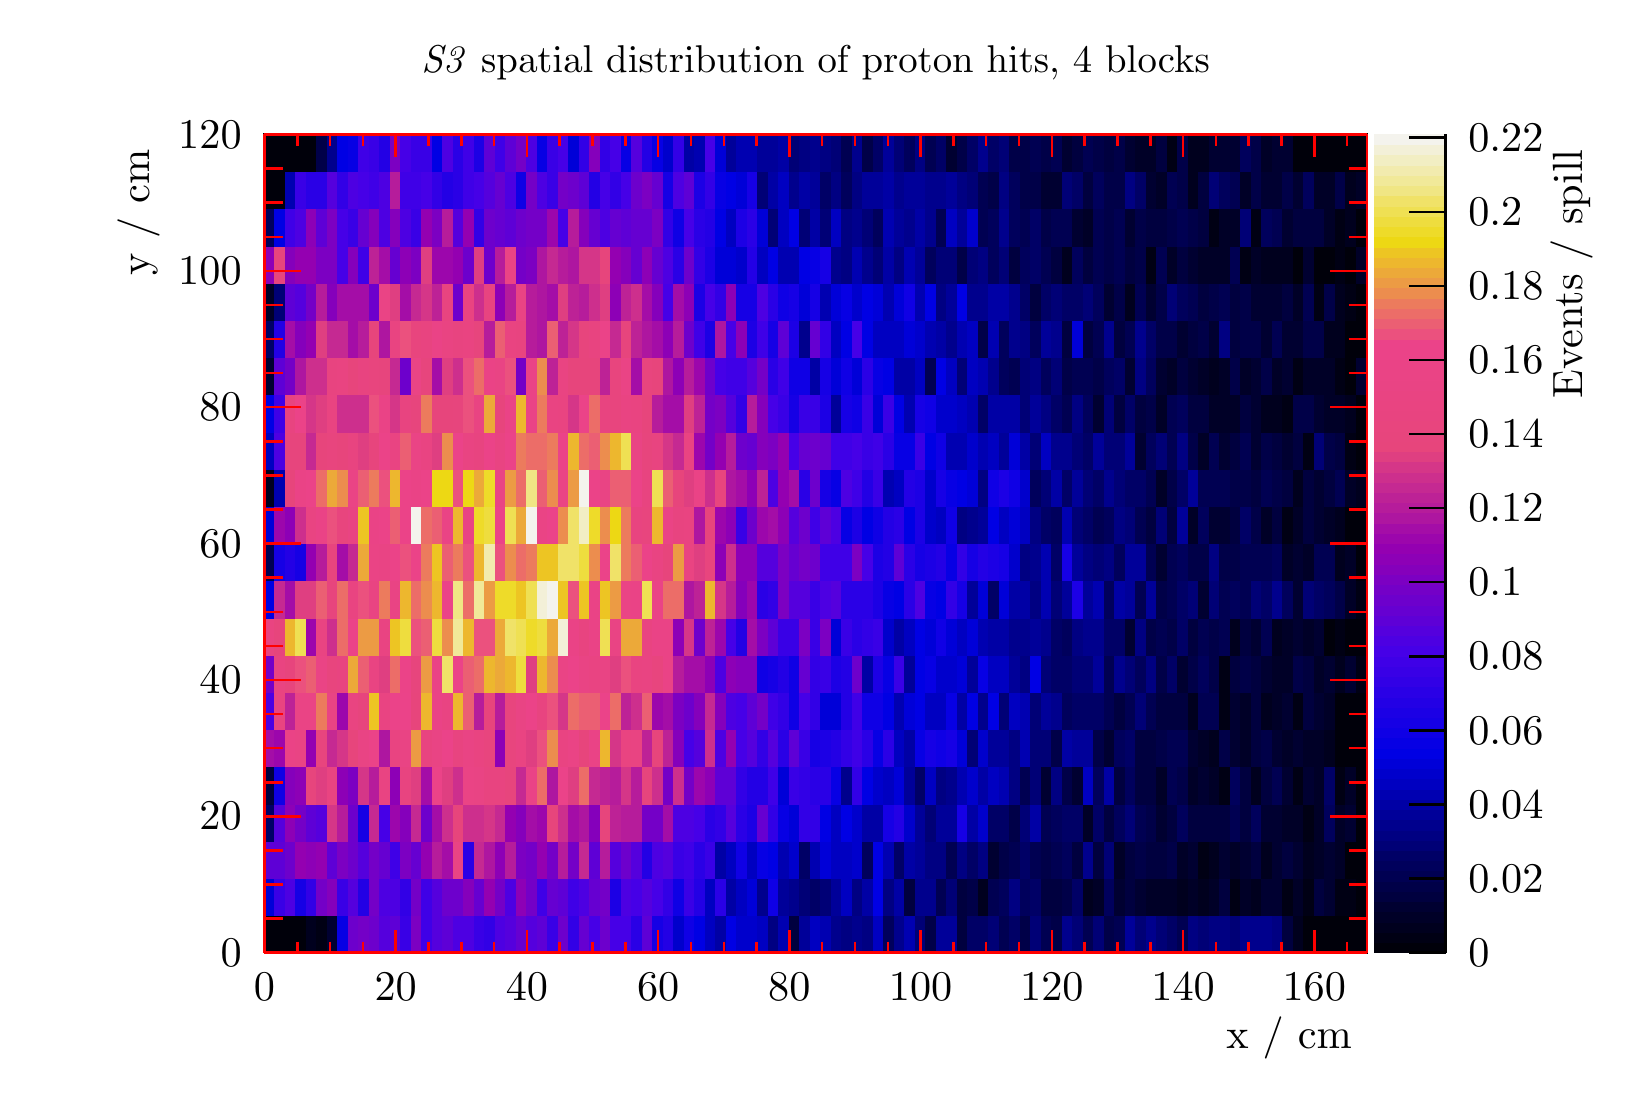
\begin{tikzpicture}
\pgfdeclareplotmark{cross} {
\pgfpathmoveto{\pgfpoint{-0.3\pgfplotmarksize}{\pgfplotmarksize}}
\pgfpathlineto{\pgfpoint{+0.3\pgfplotmarksize}{\pgfplotmarksize}}
\pgfpathlineto{\pgfpoint{+0.3\pgfplotmarksize}{0.3\pgfplotmarksize}}
\pgfpathlineto{\pgfpoint{+1\pgfplotmarksize}{0.3\pgfplotmarksize}}
\pgfpathlineto{\pgfpoint{+1\pgfplotmarksize}{-0.3\pgfplotmarksize}}
\pgfpathlineto{\pgfpoint{+0.3\pgfplotmarksize}{-0.3\pgfplotmarksize}}
\pgfpathlineto{\pgfpoint{+0.3\pgfplotmarksize}{-1.\pgfplotmarksize}}
\pgfpathlineto{\pgfpoint{-0.3\pgfplotmarksize}{-1.\pgfplotmarksize}}
\pgfpathlineto{\pgfpoint{-0.3\pgfplotmarksize}{-0.3\pgfplotmarksize}}
\pgfpathlineto{\pgfpoint{-1.\pgfplotmarksize}{-0.3\pgfplotmarksize}}
\pgfpathlineto{\pgfpoint{-1.\pgfplotmarksize}{0.3\pgfplotmarksize}}
\pgfpathlineto{\pgfpoint{-0.3\pgfplotmarksize}{0.3\pgfplotmarksize}}
\pgfpathclose
\pgfusepathqstroke
}
\pgfdeclareplotmark{cross*} {
\pgfpathmoveto{\pgfpoint{-0.3\pgfplotmarksize}{\pgfplotmarksize}}
\pgfpathlineto{\pgfpoint{+0.3\pgfplotmarksize}{\pgfplotmarksize}}
\pgfpathlineto{\pgfpoint{+0.3\pgfplotmarksize}{0.3\pgfplotmarksize}}
\pgfpathlineto{\pgfpoint{+1\pgfplotmarksize}{0.3\pgfplotmarksize}}
\pgfpathlineto{\pgfpoint{+1\pgfplotmarksize}{-0.3\pgfplotmarksize}}
\pgfpathlineto{\pgfpoint{+0.3\pgfplotmarksize}{-0.3\pgfplotmarksize}}
\pgfpathlineto{\pgfpoint{+0.3\pgfplotmarksize}{-1.\pgfplotmarksize}}
\pgfpathlineto{\pgfpoint{-0.3\pgfplotmarksize}{-1.\pgfplotmarksize}}
\pgfpathlineto{\pgfpoint{-0.3\pgfplotmarksize}{-0.3\pgfplotmarksize}}
\pgfpathlineto{\pgfpoint{-1.\pgfplotmarksize}{-0.3\pgfplotmarksize}}
\pgfpathlineto{\pgfpoint{-1.\pgfplotmarksize}{0.3\pgfplotmarksize}}
\pgfpathlineto{\pgfpoint{-0.3\pgfplotmarksize}{0.3\pgfplotmarksize}}
\pgfpathclose
\pgfusepathqfillstroke
}
\pgfdeclareplotmark{newstar} {
\pgfpathmoveto{\pgfqpoint{0pt}{\pgfplotmarksize}}
\pgfpathlineto{\pgfqpointpolar{44}{0.5\pgfplotmarksize}}
\pgfpathlineto{\pgfqpointpolar{18}{\pgfplotmarksize}}
\pgfpathlineto{\pgfqpointpolar{-20}{0.5\pgfplotmarksize}}
\pgfpathlineto{\pgfqpointpolar{-54}{\pgfplotmarksize}}
\pgfpathlineto{\pgfqpointpolar{-90}{0.5\pgfplotmarksize}}
\pgfpathlineto{\pgfqpointpolar{234}{\pgfplotmarksize}}
\pgfpathlineto{\pgfqpointpolar{198}{0.5\pgfplotmarksize}}
\pgfpathlineto{\pgfqpointpolar{162}{\pgfplotmarksize}}
\pgfpathlineto{\pgfqpointpolar{134}{0.5\pgfplotmarksize}}
\pgfpathclose
\pgfusepathqstroke
}
\pgfdeclareplotmark{newstar*} {
\pgfpathmoveto{\pgfqpoint{0pt}{\pgfplotmarksize}}
\pgfpathlineto{\pgfqpointpolar{44}{0.5\pgfplotmarksize}}
\pgfpathlineto{\pgfqpointpolar{18}{\pgfplotmarksize}}
\pgfpathlineto{\pgfqpointpolar{-20}{0.5\pgfplotmarksize}}
\pgfpathlineto{\pgfqpointpolar{-54}{\pgfplotmarksize}}
\pgfpathlineto{\pgfqpointpolar{-90}{0.5\pgfplotmarksize}}
\pgfpathlineto{\pgfqpointpolar{234}{\pgfplotmarksize}}
\pgfpathlineto{\pgfqpointpolar{198}{0.5\pgfplotmarksize}}
\pgfpathlineto{\pgfqpointpolar{162}{\pgfplotmarksize}}
\pgfpathlineto{\pgfqpointpolar{134}{0.5\pgfplotmarksize}}
\pgfpathclose
\pgfusepathqfillstroke
}
\definecolor{c}{rgb}{1,1,1};
\draw [color=c, fill=c] (0,0) rectangle (20,13.4957);
\draw [color=c, fill=c] (3,1.75444) rectangle (17,12.1461);
\definecolor{c}{rgb}{0,0,0};
\draw [c,line width=0.9] (3,1.75444) -- (3,12.1461) -- (17,12.1461) -- (17,1.75444) -- (3,1.75444);
\definecolor{c}{rgb}{1,1,1};
\draw [color=c, fill=c] (3,1.75444) rectangle (17,12.1461);
\definecolor{c}{rgb}{0,0,0};
\draw [c,line width=0.9] (3,1.75444) -- (3,12.1461) -- (17,12.1461) -- (17,1.75444) -- (3,1.75444);
\definecolor{c}{rgb}{0,0,0.0387097};
\draw [color=c, fill=c] (3,1.75444) rectangle (3.13333,2.22679);
\draw [color=c, fill=c] (3.13333,1.75444) rectangle (3.26667,2.22679);
\draw [color=c, fill=c] (3.26667,1.75444) rectangle (3.4,2.22679);
\draw [color=c, fill=c] (3.4,1.75444) rectangle (3.53333,2.22679);
\definecolor{c}{rgb}{0,0,0.116129};
\draw [color=c, fill=c] (3.53333,1.75444) rectangle (3.66667,2.22679);
\definecolor{c}{rgb}{0,0,0.0774194};
\draw [color=c, fill=c] (3.66667,1.75444) rectangle (3.8,2.22679);
\definecolor{c}{rgb}{0,0,0.193548};
\draw [color=c, fill=c] (3.8,1.75444) rectangle (3.93333,2.22679);
\definecolor{c}{rgb}{0.0257353,0,0.895221};
\draw [color=c, fill=c] (3.93333,1.75444) rectangle (4.06667,2.22679);
\definecolor{c}{rgb}{0.427451,0,0.8};
\draw [color=c, fill=c] (4.06667,1.75444) rectangle (4.2,2.22679);
\definecolor{c}{rgb}{0.456127,0,0.780147};
\draw [color=c, fill=c] (4.2,1.75444) rectangle (4.33333,2.22679);
\definecolor{c}{rgb}{0.427451,0,0.8};
\draw [color=c, fill=c] (4.33333,1.75444) rectangle (4.46667,2.22679);
\definecolor{c}{rgb}{0.331863,0,0.866176};
\draw [color=c, fill=c] (4.46667,1.75444) rectangle (4.6,2.22679);
\definecolor{c}{rgb}{0.370098,0,0.839706};
\draw [color=c, fill=c] (4.6,1.75444) rectangle (4.73333,2.22679);
\definecolor{c}{rgb}{0.223039,0,0.903676};
\draw [color=c, fill=c] (4.73333,1.75444) rectangle (4.86667,2.22679);
\definecolor{c}{rgb}{0.484804,0,0.760294};
\draw [color=c, fill=c] (4.86667,1.75444) rectangle (5,2.22679);
\definecolor{c}{rgb}{0.248775,0,0.904779};
\draw [color=c, fill=c] (5,1.75444) rectangle (5.13333,2.22679);
\definecolor{c}{rgb}{0.331863,0,0.866176};
\draw [color=c, fill=c] (5.13333,1.75444) rectangle (5.26667,2.22679);
\definecolor{c}{rgb}{0.370098,0,0.839706};
\draw [color=c, fill=c] (5.26667,1.75444) rectangle (5.4,2.22679);
\definecolor{c}{rgb}{0.303186,0,0.886029};
\draw [color=c, fill=c] (5.4,1.75444) rectangle (5.53333,2.22679);
\draw [color=c, fill=c] (5.53333,1.75444) rectangle (5.66667,2.22679);
\definecolor{c}{rgb}{0.223039,0,0.903676};
\draw [color=c, fill=c] (5.66667,1.75444) rectangle (5.8,2.22679);
\definecolor{c}{rgb}{0.197304,0,0.902574};
\draw [color=c, fill=c] (5.8,1.75444) rectangle (5.93333,2.22679);
\definecolor{c}{rgb}{0.303186,0,0.886029};
\draw [color=c, fill=c] (5.93333,1.75444) rectangle (6.06667,2.22679);
\definecolor{c}{rgb}{0.331863,0,0.866176};
\draw [color=c, fill=c] (6.06667,1.75444) rectangle (6.2,2.22679);
\definecolor{c}{rgb}{0.398775,0,0.819853};
\draw [color=c, fill=c] (6.2,1.75444) rectangle (6.33333,2.22679);
\definecolor{c}{rgb}{0.331863,0,0.866176};
\draw [color=c, fill=c] (6.33333,1.75444) rectangle (6.46667,2.22679);
\definecolor{c}{rgb}{0.370098,0,0.839706};
\draw [color=c, fill=c] (6.46667,1.75444) rectangle (6.6,2.22679);
\definecolor{c}{rgb}{0.223039,0,0.903676};
\draw [color=c, fill=c] (6.6,1.75444) rectangle (6.73333,2.22679);
\definecolor{c}{rgb}{0.427451,0,0.8};
\draw [color=c, fill=c] (6.73333,1.75444) rectangle (6.86667,2.22679);
\definecolor{c}{rgb}{0.197304,0,0.902574};
\draw [color=c, fill=c] (6.86667,1.75444) rectangle (7,2.22679);
\definecolor{c}{rgb}{0.398775,0,0.819853};
\draw [color=c, fill=c] (7,1.75444) rectangle (7.13333,2.22679);
\definecolor{c}{rgb}{0.27451,0,0.905882};
\draw [color=c, fill=c] (7.13333,1.75444) rectangle (7.26667,2.22679);
\definecolor{c}{rgb}{0.427451,0,0.8};
\draw [color=c, fill=c] (7.26667,1.75444) rectangle (7.4,2.22679);
\definecolor{c}{rgb}{0.27451,0,0.905882};
\draw [color=c, fill=c] (7.4,1.75444) rectangle (7.53333,2.22679);
\draw [color=c, fill=c] (7.53333,1.75444) rectangle (7.66667,2.22679);
\definecolor{c}{rgb}{0.16299,0,0.901103};
\draw [color=c, fill=c] (7.66667,1.75444) rectangle (7.8,2.22679);
\definecolor{c}{rgb}{0.370098,0,0.839706};
\draw [color=c, fill=c] (7.8,1.75444) rectangle (7.93333,2.22679);
\definecolor{c}{rgb}{0.0857843,0,0.897794};
\draw [color=c, fill=c] (7.93333,1.75444) rectangle (8.06667,2.22679);
\definecolor{c}{rgb}{0.137255,0,0.9};
\draw [color=c, fill=c] (8.06667,1.75444) rectangle (8.2,2.22679);
\definecolor{c}{rgb}{0,0,0.801471};
\draw [color=c, fill=c] (8.2,1.75444) rectangle (8.33333,2.22679);
\definecolor{c}{rgb}{0.060049,0,0.896691};
\draw [color=c, fill=c] (8.33333,1.75444) rectangle (8.46667,2.22679);
\definecolor{c}{rgb}{0,0,0.894118};
\draw [color=c, fill=c] (8.46667,1.75444) rectangle (8.6,2.22679);
\definecolor{c}{rgb}{0,0,0.755147};
\draw [color=c, fill=c] (8.6,1.75444) rectangle (8.73333,2.22679);
\definecolor{c}{rgb}{0,0,0.647059};
\draw [color=c, fill=c] (8.73333,1.75444) rectangle (8.86667,2.22679);
\definecolor{c}{rgb}{0,0,0.894118};
\draw [color=c, fill=c] (8.86667,1.75444) rectangle (9,2.22679);
\definecolor{c}{rgb}{0,0,0.801471};
\draw [color=c, fill=c] (9,1.75444) rectangle (9.13333,2.22679);
\draw [color=c, fill=c] (9.13333,1.75444) rectangle (9.26667,2.22679);
\definecolor{c}{rgb}{0,0,0.755147};
\draw [color=c, fill=c] (9.26667,1.75444) rectangle (9.4,2.22679);
\definecolor{c}{rgb}{0,0,0.508088};
\draw [color=c, fill=c] (9.4,1.75444) rectangle (9.53333,2.22679);
\definecolor{c}{rgb}{0,0,0.693382};
\draw [color=c, fill=c] (9.53333,1.75444) rectangle (9.66667,2.22679);
\definecolor{c}{rgb}{0,0,0.245161};
\draw [color=c, fill=c] (9.66667,1.75444) rectangle (9.8,2.22679);
\definecolor{c}{rgb}{0,0,0.600735};
\draw [color=c, fill=c] (9.8,1.75444) rectangle (9.93333,2.22679);
\definecolor{c}{rgb}{0,0,0.755147};
\draw [color=c, fill=c] (9.93333,1.75444) rectangle (10.0667,2.22679);
\definecolor{c}{rgb}{0,0,0.693382};
\draw [color=c, fill=c] (10.0667,1.75444) rectangle (10.2,2.22679);
\definecolor{c}{rgb}{0,0,0.554412};
\draw [color=c, fill=c] (10.2,1.75444) rectangle (10.3333,2.22679);
\definecolor{c}{rgb}{0,0,0.508088};
\draw [color=c, fill=c] (10.3333,1.75444) rectangle (10.4667,2.22679);
\definecolor{c}{rgb}{0,0,0.554412};
\draw [color=c, fill=c] (10.4667,1.75444) rectangle (10.6,2.22679);
\definecolor{c}{rgb}{0,0,0.508088};
\draw [color=c, fill=c] (10.6,1.75444) rectangle (10.7333,2.22679);
\definecolor{c}{rgb}{0,0,0.755147};
\draw [color=c, fill=c] (10.7333,1.75444) rectangle (10.8667,2.22679);
\definecolor{c}{rgb}{0,0,0.36129};
\draw [color=c, fill=c] (10.8667,1.75444) rectangle (11,2.22679);
\definecolor{c}{rgb}{0,0,0.554412};
\draw [color=c, fill=c] (11,1.75444) rectangle (11.1333,2.22679);
\definecolor{c}{rgb}{0,0,0.693382};
\draw [color=c, fill=c] (11.1333,1.75444) rectangle (11.2667,2.22679);
\definecolor{c}{rgb}{0,0,0.461765};
\draw [color=c, fill=c] (11.2667,1.75444) rectangle (11.4,2.22679);
\definecolor{c}{rgb}{0,0,0.283871};
\draw [color=c, fill=c] (11.4,1.75444) rectangle (11.5333,2.22679);
\definecolor{c}{rgb}{0,0,0.600735};
\draw [color=c, fill=c] (11.5333,1.75444) rectangle (11.6667,2.22679);
\draw [color=c, fill=c] (11.6667,1.75444) rectangle (11.8,2.22679);
\definecolor{c}{rgb}{0,0,0.245161};
\draw [color=c, fill=c] (11.8,1.75444) rectangle (11.9333,2.22679);
\definecolor{c}{rgb}{0,0,0.4};
\draw [color=c, fill=c] (11.9333,1.75444) rectangle (12.0667,2.22679);
\draw [color=c, fill=c] (12.0667,1.75444) rectangle (12.2,2.22679);
\definecolor{c}{rgb}{0,0,0.461765};
\draw [color=c, fill=c] (12.2,1.75444) rectangle (12.3333,2.22679);
\definecolor{c}{rgb}{0,0,0.322581};
\draw [color=c, fill=c] (12.3333,1.75444) rectangle (12.4667,2.22679);
\definecolor{c}{rgb}{0,0,0.4};
\draw [color=c, fill=c] (12.4667,1.75444) rectangle (12.6,2.22679);
\definecolor{c}{rgb}{0,0,0.283871};
\draw [color=c, fill=c] (12.6,1.75444) rectangle (12.7333,2.22679);
\definecolor{c}{rgb}{0,0,0.461765};
\draw [color=c, fill=c] (12.7333,1.75444) rectangle (12.8667,2.22679);
\definecolor{c}{rgb}{0,0,0.322581};
\draw [color=c, fill=c] (12.8667,1.75444) rectangle (13,2.22679);
\definecolor{c}{rgb}{0,0,0.283871};
\draw [color=c, fill=c] (13,1.75444) rectangle (13.1333,2.22679);
\definecolor{c}{rgb}{0,0,0.554412};
\draw [color=c, fill=c] (13.1333,1.75444) rectangle (13.2667,2.22679);
\definecolor{c}{rgb}{0,0,0.461765};
\draw [color=c, fill=c] (13.2667,1.75444) rectangle (13.4,2.22679);
\definecolor{c}{rgb}{0,0,0.322581};
\draw [color=c, fill=c] (13.4,1.75444) rectangle (13.5333,2.22679);
\definecolor{c}{rgb}{0,0,0.461765};
\draw [color=c, fill=c] (13.5333,1.75444) rectangle (13.6667,2.22679);
\definecolor{c}{rgb}{0,0,0.283871};
\draw [color=c, fill=c] (13.6667,1.75444) rectangle (13.8,2.22679);
\definecolor{c}{rgb}{0,0,0.322581};
\draw [color=c, fill=c] (13.8,1.75444) rectangle (13.9333,2.22679);
\definecolor{c}{rgb}{0,0,0.600735};
\draw [color=c, fill=c] (13.9333,1.75444) rectangle (14.0667,2.22679);
\definecolor{c}{rgb}{0,0,0.461765};
\draw [color=c, fill=c] (14.0667,1.75444) rectangle (14.2,2.22679);
\definecolor{c}{rgb}{0,0,0.554412};
\draw [color=c, fill=c] (14.2,1.75444) rectangle (14.3333,2.22679);
\definecolor{c}{rgb}{0,0,0.461765};
\draw [color=c, fill=c] (14.3333,1.75444) rectangle (14.4667,2.22679);
\definecolor{c}{rgb}{0,0,0.4};
\draw [color=c, fill=c] (14.4667,1.75444) rectangle (14.6,2.22679);
\definecolor{c}{rgb}{0,0,0.322581};
\draw [color=c, fill=c] (14.6,1.75444) rectangle (14.7333,2.22679);
\definecolor{c}{rgb}{0,0,0.508088};
\draw [color=c, fill=c] (14.7333,1.75444) rectangle (14.8667,2.22679);
\definecolor{c}{rgb}{0,0,0.461765};
\draw [color=c, fill=c] (14.8667,1.75444) rectangle (15,2.22679);
\definecolor{c}{rgb}{0,0,0.508088};
\draw [color=c, fill=c] (15,1.75444) rectangle (15.1333,2.22679);
\draw [color=c, fill=c] (15.1333,1.75444) rectangle (15.2667,2.22679);
\definecolor{c}{rgb}{0,0,0.461765};
\draw [color=c, fill=c] (15.2667,1.75444) rectangle (15.4,2.22679);
\definecolor{c}{rgb}{0,0,0.554412};
\draw [color=c, fill=c] (15.4,1.75444) rectangle (15.5333,2.22679);
\draw [color=c, fill=c] (15.5333,1.75444) rectangle (15.6667,2.22679);
\draw [color=c, fill=c] (15.6667,1.75444) rectangle (15.8,2.22679);
\definecolor{c}{rgb}{0,0,0.508088};
\draw [color=c, fill=c] (15.8,1.75444) rectangle (15.9333,2.22679);
\definecolor{c}{rgb}{0,0,0.245161};
\draw [color=c, fill=c] (15.9333,1.75444) rectangle (16.0667,2.22679);
\definecolor{c}{rgb}{0,0,0.116129};
\draw [color=c, fill=c] (16.0667,1.75444) rectangle (16.2,2.22679);
\definecolor{c}{rgb}{0,0,0.0387097};
\draw [color=c, fill=c] (16.2,1.75444) rectangle (16.3333,2.22679);
\draw [color=c, fill=c] (16.3333,1.75444) rectangle (16.4667,2.22679);
\draw [color=c, fill=c] (16.4667,1.75444) rectangle (16.6,2.22679);
\draw [color=c, fill=c] (16.6,1.75444) rectangle (16.7333,2.22679);
\draw [color=c, fill=c] (16.7333,1.75444) rectangle (16.8667,2.22679);
\draw [color=c, fill=c] (16.8667,1.75444) rectangle (17,2.22679);
\definecolor{c}{rgb}{0,0,0.847794};
\draw [color=c, fill=c] (3,2.22679) rectangle (3.13333,2.69914);
\definecolor{c}{rgb}{0.223039,0,0.903676};
\draw [color=c, fill=c] (3.13333,2.22679) rectangle (3.26667,2.69914);
\definecolor{c}{rgb}{0.303186,0,0.886029};
\draw [color=c, fill=c] (3.26667,2.22679) rectangle (3.4,2.69914);
\definecolor{c}{rgb}{0.0857843,0,0.897794};
\draw [color=c, fill=c] (3.4,2.22679) rectangle (3.53333,2.69914);
\definecolor{c}{rgb}{0.197304,0,0.902574};
\draw [color=c, fill=c] (3.53333,2.22679) rectangle (3.66667,2.69914);
\definecolor{c}{rgb}{0.456127,0,0.780147};
\draw [color=c, fill=c] (3.66667,2.22679) rectangle (3.8,2.69914);
\definecolor{c}{rgb}{0.523039,0,0.733824};
\draw [color=c, fill=c] (3.8,2.22679) rectangle (3.93333,2.69914);
\definecolor{c}{rgb}{0.223039,0,0.903676};
\draw [color=c, fill=c] (3.93333,2.22679) rectangle (4.06667,2.69914);
\definecolor{c}{rgb}{0.331863,0,0.866176};
\draw [color=c, fill=c] (4.06667,2.22679) rectangle (4.2,2.69914);
\definecolor{c}{rgb}{0.137255,0,0.9};
\draw [color=c, fill=c] (4.2,2.22679) rectangle (4.33333,2.69914);
\definecolor{c}{rgb}{0.456127,0,0.780147};
\draw [color=c, fill=c] (4.33333,2.22679) rectangle (4.46667,2.69914);
\definecolor{c}{rgb}{0.303186,0,0.886029};
\draw [color=c, fill=c] (4.46667,2.22679) rectangle (4.6,2.69914);
\draw [color=c, fill=c] (4.6,2.22679) rectangle (4.73333,2.69914);
\definecolor{c}{rgb}{0.197304,0,0.902574};
\draw [color=c, fill=c] (4.73333,2.22679) rectangle (4.86667,2.69914);
\definecolor{c}{rgb}{0.456127,0,0.780147};
\draw [color=c, fill=c] (4.86667,2.22679) rectangle (5,2.69914);
\definecolor{c}{rgb}{0.248775,0,0.904779};
\draw [color=c, fill=c] (5,2.22679) rectangle (5.13333,2.69914);
\definecolor{c}{rgb}{0.331863,0,0.866176};
\draw [color=c, fill=c] (5.13333,2.22679) rectangle (5.26667,2.69914);
\definecolor{c}{rgb}{0.427451,0,0.8};
\draw [color=c, fill=c] (5.26667,2.22679) rectangle (5.4,2.69914);
\draw [color=c, fill=c] (5.4,2.22679) rectangle (5.53333,2.69914);
\definecolor{c}{rgb}{0.523039,0,0.733824};
\draw [color=c, fill=c] (5.53333,2.22679) rectangle (5.66667,2.69914);
\definecolor{c}{rgb}{0.398775,0,0.819853};
\draw [color=c, fill=c] (5.66667,2.22679) rectangle (5.8,2.69914);
\definecolor{c}{rgb}{0.580392,0,0.694118};
\draw [color=c, fill=c] (5.8,2.22679) rectangle (5.93333,2.69914);
\definecolor{c}{rgb}{0.456127,0,0.780147};
\draw [color=c, fill=c] (5.93333,2.22679) rectangle (6.06667,2.69914);
\definecolor{c}{rgb}{0.303186,0,0.886029};
\draw [color=c, fill=c] (6.06667,2.22679) rectangle (6.2,2.69914);
\definecolor{c}{rgb}{0.551716,0,0.713971};
\draw [color=c, fill=c] (6.2,2.22679) rectangle (6.33333,2.69914);
\definecolor{c}{rgb}{0.456127,0,0.780147};
\draw [color=c, fill=c] (6.33333,2.22679) rectangle (6.46667,2.69914);
\definecolor{c}{rgb}{0.248775,0,0.904779};
\draw [color=c, fill=c] (6.46667,2.22679) rectangle (6.6,2.69914);
\definecolor{c}{rgb}{0.398775,0,0.819853};
\draw [color=c, fill=c] (6.6,2.22679) rectangle (6.73333,2.69914);
\definecolor{c}{rgb}{0.370098,0,0.839706};
\draw [color=c, fill=c] (6.73333,2.22679) rectangle (6.86667,2.69914);
\definecolor{c}{rgb}{0.248775,0,0.904779};
\draw [color=c, fill=c] (6.86667,2.22679) rectangle (7,2.69914);
\definecolor{c}{rgb}{0.303186,0,0.886029};
\draw [color=c, fill=c] (7,2.22679) rectangle (7.13333,2.69914);
\definecolor{c}{rgb}{0.398775,0,0.819853};
\draw [color=c, fill=c] (7.13333,2.22679) rectangle (7.26667,2.69914);
\definecolor{c}{rgb}{0.456127,0,0.780147};
\draw [color=c, fill=c] (7.26667,2.22679) rectangle (7.4,2.69914);
\definecolor{c}{rgb}{0.11152,0,0.898897};
\draw [color=c, fill=c] (7.4,2.22679) rectangle (7.53333,2.69914);
\definecolor{c}{rgb}{0.303186,0,0.886029};
\draw [color=c, fill=c] (7.53333,2.22679) rectangle (7.66667,2.69914);
\definecolor{c}{rgb}{0.27451,0,0.905882};
\draw [color=c, fill=c] (7.66667,2.22679) rectangle (7.8,2.69914);
\definecolor{c}{rgb}{0.331863,0,0.866176};
\draw [color=c, fill=c] (7.8,2.22679) rectangle (7.93333,2.69914);
\definecolor{c}{rgb}{0.27451,0,0.905882};
\draw [color=c, fill=c] (7.93333,2.22679) rectangle (8.06667,2.69914);
\definecolor{c}{rgb}{0.197304,0,0.902574};
\draw [color=c, fill=c] (8.06667,2.22679) rectangle (8.2,2.69914);
\definecolor{c}{rgb}{0.060049,0,0.896691};
\draw [color=c, fill=c] (8.2,2.22679) rectangle (8.33333,2.69914);
\definecolor{c}{rgb}{0.223039,0,0.903676};
\draw [color=c, fill=c] (8.33333,2.22679) rectangle (8.46667,2.69914);
\definecolor{c}{rgb}{0.137255,0,0.9};
\draw [color=c, fill=c] (8.46667,2.22679) rectangle (8.6,2.69914);
\definecolor{c}{rgb}{0,0,0.755147};
\draw [color=c, fill=c] (8.6,2.22679) rectangle (8.73333,2.69914);
\definecolor{c}{rgb}{0.16299,0,0.901103};
\draw [color=c, fill=c] (8.73333,2.22679) rectangle (8.86667,2.69914);
\definecolor{c}{rgb}{0,0,0.647059};
\draw [color=c, fill=c] (8.86667,2.22679) rectangle (9,2.69914);
\definecolor{c}{rgb}{0,0,0.755147};
\draw [color=c, fill=c] (9,2.22679) rectangle (9.13333,2.69914);
\definecolor{c}{rgb}{0,0,0.847794};
\draw [color=c, fill=c] (9.13333,2.22679) rectangle (9.26667,2.69914);
\definecolor{c}{rgb}{0,0,0.554412};
\draw [color=c, fill=c] (9.26667,2.22679) rectangle (9.4,2.69914);
\definecolor{c}{rgb}{0.060049,0,0.896691};
\draw [color=c, fill=c] (9.4,2.22679) rectangle (9.53333,2.69914);
\definecolor{c}{rgb}{0,0,0.600735};
\draw [color=c, fill=c] (9.53333,2.22679) rectangle (9.66667,2.69914);
\definecolor{c}{rgb}{0,0,0.554412};
\draw [color=c, fill=c] (9.66667,2.22679) rectangle (9.8,2.69914);
\definecolor{c}{rgb}{0,0,0.461765};
\draw [color=c, fill=c] (9.8,2.22679) rectangle (9.93333,2.69914);
\definecolor{c}{rgb}{0,0,0.4};
\draw [color=c, fill=c] (9.93333,2.22679) rectangle (10.0667,2.69914);
\definecolor{c}{rgb}{0,0,0.461765};
\draw [color=c, fill=c] (10.0667,2.22679) rectangle (10.2,2.69914);
\definecolor{c}{rgb}{0,0,0.600735};
\draw [color=c, fill=c] (10.2,2.22679) rectangle (10.3333,2.69914);
\definecolor{c}{rgb}{0,0,0.755147};
\draw [color=c, fill=c] (10.3333,2.22679) rectangle (10.4667,2.69914);
\definecolor{c}{rgb}{0,0,0.508088};
\draw [color=c, fill=c] (10.4667,2.22679) rectangle (10.6,2.69914);
\definecolor{c}{rgb}{0,0,0.647059};
\draw [color=c, fill=c] (10.6,2.22679) rectangle (10.7333,2.69914);
\definecolor{c}{rgb}{0,0,0.894118};
\draw [color=c, fill=c] (10.7333,2.22679) rectangle (10.8667,2.69914);
\definecolor{c}{rgb}{0,0,0.508088};
\draw [color=c, fill=c] (10.8667,2.22679) rectangle (11,2.69914);
\definecolor{c}{rgb}{0,0,0.647059};
\draw [color=c, fill=c] (11,2.22679) rectangle (11.1333,2.69914);
\definecolor{c}{rgb}{0,0,0.245161};
\draw [color=c, fill=c] (11.1333,2.22679) rectangle (11.2667,2.69914);
\definecolor{c}{rgb}{0,0,0.554412};
\draw [color=c, fill=c] (11.2667,2.22679) rectangle (11.4,2.69914);
\draw [color=c, fill=c] (11.4,2.22679) rectangle (11.5333,2.69914);
\definecolor{c}{rgb}{0,0,0.322581};
\draw [color=c, fill=c] (11.5333,2.22679) rectangle (11.6667,2.69914);
\definecolor{c}{rgb}{0,0,0.461765};
\draw [color=c, fill=c] (11.6667,2.22679) rectangle (11.8,2.69914);
\definecolor{c}{rgb}{0,0,0.245161};
\draw [color=c, fill=c] (11.8,2.22679) rectangle (11.9333,2.69914);
\definecolor{c}{rgb}{0,0,0.283871};
\draw [color=c, fill=c] (11.9333,2.22679) rectangle (12.0667,2.69914);
\definecolor{c}{rgb}{0,0,0.116129};
\draw [color=c, fill=c] (12.0667,2.22679) rectangle (12.2,2.69914);
\definecolor{c}{rgb}{0,0,0.322581};
\draw [color=c, fill=c] (12.2,2.22679) rectangle (12.3333,2.69914);
\definecolor{c}{rgb}{0,0,0.36129};
\draw [color=c, fill=c] (12.3333,2.22679) rectangle (12.4667,2.69914);
\definecolor{c}{rgb}{0,0,0.508088};
\draw [color=c, fill=c] (12.4667,2.22679) rectangle (12.6,2.69914);
\definecolor{c}{rgb}{0,0,0.36129};
\draw [color=c, fill=c] (12.6,2.22679) rectangle (12.7333,2.69914);
\definecolor{c}{rgb}{0,0,0.4};
\draw [color=c, fill=c] (12.7333,2.22679) rectangle (12.8667,2.69914);
\definecolor{c}{rgb}{0,0,0.245161};
\draw [color=c, fill=c] (12.8667,2.22679) rectangle (13,2.69914);
\draw [color=c, fill=c] (13,2.22679) rectangle (13.1333,2.69914);
\definecolor{c}{rgb}{0,0,0.283871};
\draw [color=c, fill=c] (13.1333,2.22679) rectangle (13.2667,2.69914);
\definecolor{c}{rgb}{0,0,0.4};
\draw [color=c, fill=c] (13.2667,2.22679) rectangle (13.4,2.69914);
\definecolor{c}{rgb}{0,0,0.116129};
\draw [color=c, fill=c] (13.4,2.22679) rectangle (13.5333,2.69914);
\definecolor{c}{rgb}{0,0,0.154839};
\draw [color=c, fill=c] (13.5333,2.22679) rectangle (13.6667,2.69914);
\definecolor{c}{rgb}{0,0,0.36129};
\draw [color=c, fill=c] (13.6667,2.22679) rectangle (13.8,2.69914);
\definecolor{c}{rgb}{0,0,0.193548};
\draw [color=c, fill=c] (13.8,2.22679) rectangle (13.9333,2.69914);
\definecolor{c}{rgb}{0,0,0.245161};
\draw [color=c, fill=c] (13.9333,2.22679) rectangle (14.0667,2.69914);
\definecolor{c}{rgb}{0,0,0.193548};
\draw [color=c, fill=c] (14.0667,2.22679) rectangle (14.2,2.69914);
\definecolor{c}{rgb}{0,0,0.154839};
\draw [color=c, fill=c] (14.2,2.22679) rectangle (14.3333,2.69914);
\draw [color=c, fill=c] (14.3333,2.22679) rectangle (14.4667,2.69914);
\draw [color=c, fill=c] (14.4667,2.22679) rectangle (14.6,2.69914);
\definecolor{c}{rgb}{0,0,0.116129};
\draw [color=c, fill=c] (14.6,2.22679) rectangle (14.7333,2.69914);
\definecolor{c}{rgb}{0,0,0.154839};
\draw [color=c, fill=c] (14.7333,2.22679) rectangle (14.8667,2.69914);
\definecolor{c}{rgb}{0,0,0.116129};
\draw [color=c, fill=c] (14.8667,2.22679) rectangle (15,2.69914);
\definecolor{c}{rgb}{0,0,0.154839};
\draw [color=c, fill=c] (15,2.22679) rectangle (15.1333,2.69914);
\definecolor{c}{rgb}{0,0,0.245161};
\draw [color=c, fill=c] (15.1333,2.22679) rectangle (15.2667,2.69914);
\definecolor{c}{rgb}{0,0,0.0774194};
\draw [color=c, fill=c] (15.2667,2.22679) rectangle (15.4,2.69914);
\definecolor{c}{rgb}{0,0,0.154839};
\draw [color=c, fill=c] (15.4,2.22679) rectangle (15.5333,2.69914);
\definecolor{c}{rgb}{0,0,0.116129};
\draw [color=c, fill=c] (15.5333,2.22679) rectangle (15.6667,2.69914);
\definecolor{c}{rgb}{0,0,0.193548};
\draw [color=c, fill=c] (15.6667,2.22679) rectangle (15.8,2.69914);
\draw [color=c, fill=c] (15.8,2.22679) rectangle (15.9333,2.69914);
\definecolor{c}{rgb}{0,0,0.0774194};
\draw [color=c, fill=c] (15.9333,2.22679) rectangle (16.0667,2.69914);
\definecolor{c}{rgb}{0,0,0.154839};
\draw [color=c, fill=c] (16.0667,2.22679) rectangle (16.2,2.69914);
\definecolor{c}{rgb}{0,0,0.0774194};
\draw [color=c, fill=c] (16.2,2.22679) rectangle (16.3333,2.69914);
\definecolor{c}{rgb}{0,0,0.245161};
\draw [color=c, fill=c] (16.3333,2.22679) rectangle (16.4667,2.69914);
\definecolor{c}{rgb}{0,0,0.193548};
\draw [color=c, fill=c] (16.4667,2.22679) rectangle (16.6,2.69914);
\definecolor{c}{rgb}{0,0,0.0774194};
\draw [color=c, fill=c] (16.6,2.22679) rectangle (16.7333,2.69914);
\draw [color=c, fill=c] (16.7333,2.22679) rectangle (16.8667,2.69914);
\definecolor{c}{rgb}{0,0,0.0387097};
\draw [color=c, fill=c] (16.8667,2.22679) rectangle (17,2.69914);
\definecolor{c}{rgb}{0.370098,0,0.839706};
\draw [color=c, fill=c] (3,2.69914) rectangle (3.13333,3.17149);
\draw [color=c, fill=c] (3.13333,2.69914) rectangle (3.26667,3.17149);
\definecolor{c}{rgb}{0.427451,0,0.8};
\draw [color=c, fill=c] (3.26667,2.69914) rectangle (3.4,3.17149);
\definecolor{c}{rgb}{0.580392,0,0.694118};
\draw [color=c, fill=c] (3.4,2.69914) rectangle (3.53333,3.17149);
\definecolor{c}{rgb}{0.551716,0,0.713971};
\draw [color=c, fill=c] (3.53333,2.69914) rectangle (3.66667,3.17149);
\definecolor{c}{rgb}{0.580392,0,0.694118};
\draw [color=c, fill=c] (3.66667,2.69914) rectangle (3.8,3.17149);
\definecolor{c}{rgb}{0.370098,0,0.839706};
\draw [color=c, fill=c] (3.8,2.69914) rectangle (3.93333,3.17149);
\definecolor{c}{rgb}{0.484804,0,0.760294};
\draw [color=c, fill=c] (3.93333,2.69914) rectangle (4.06667,3.17149);
\definecolor{c}{rgb}{0.427451,0,0.8};
\draw [color=c, fill=c] (4.06667,2.69914) rectangle (4.2,3.17149);
\definecolor{c}{rgb}{0.331863,0,0.866176};
\draw [color=c, fill=c] (4.2,2.69914) rectangle (4.33333,3.17149);
\definecolor{c}{rgb}{0.456127,0,0.780147};
\draw [color=c, fill=c] (4.33333,2.69914) rectangle (4.46667,3.17149);
\definecolor{c}{rgb}{0.398775,0,0.819853};
\draw [color=c, fill=c] (4.46667,2.69914) rectangle (4.6,3.17149);
\definecolor{c}{rgb}{0.248775,0,0.904779};
\draw [color=c, fill=c] (4.6,2.69914) rectangle (4.73333,3.17149);
\definecolor{c}{rgb}{0.484804,0,0.760294};
\draw [color=c, fill=c] (4.73333,2.69914) rectangle (4.86667,3.17149);
\definecolor{c}{rgb}{0.398775,0,0.819853};
\draw [color=c, fill=c] (4.86667,2.69914) rectangle (5,3.17149);
\definecolor{c}{rgb}{0.580392,0,0.694118};
\draw [color=c, fill=c] (5,2.69914) rectangle (5.13333,3.17149);
\definecolor{c}{rgb}{0.712623,0.109926,0.609681};
\draw [color=c, fill=c] (5.13333,2.69914) rectangle (5.26667,3.17149);
\definecolor{c}{rgb}{0.641422,0.0507353,0.655147};
\draw [color=c, fill=c] (5.26667,2.69914) rectangle (5.4,3.17149);
\definecolor{c}{rgb}{0.915196,0.265931,0.516544};
\draw [color=c, fill=c] (5.4,2.69914) rectangle (5.53333,3.17149);
\definecolor{c}{rgb}{0.16299,0,0.901103};
\draw [color=c, fill=c] (5.53333,2.69914) rectangle (5.66667,3.17149);
\definecolor{c}{rgb}{0.773652,0.160662,0.570711};
\draw [color=c, fill=c] (5.66667,2.69914) rectangle (5.8,3.17149);
\definecolor{c}{rgb}{0.682108,0.0845588,0.629167};
\draw [color=c, fill=c] (5.8,2.69914) rectangle (5.93333,3.17149);
\definecolor{c}{rgb}{0.551716,0,0.713971};
\draw [color=c, fill=c] (5.93333,2.69914) rectangle (6.06667,3.17149);
\definecolor{c}{rgb}{0.712623,0.109926,0.609681};
\draw [color=c, fill=c] (6.06667,2.69914) rectangle (6.2,3.17149);
\definecolor{c}{rgb}{0.484804,0,0.760294};
\draw [color=c, fill=c] (6.2,2.69914) rectangle (6.33333,3.17149);
\definecolor{c}{rgb}{0.456127,0,0.780147};
\draw [color=c, fill=c] (6.33333,2.69914) rectangle (6.46667,3.17149);
\definecolor{c}{rgb}{0.580392,0,0.694118};
\draw [color=c, fill=c] (6.46667,2.69914) rectangle (6.6,3.17149);
\definecolor{c}{rgb}{0.456127,0,0.780147};
\draw [color=c, fill=c] (6.6,2.69914) rectangle (6.73333,3.17149);
\definecolor{c}{rgb}{0.712623,0.109926,0.609681};
\draw [color=c, fill=c] (6.73333,2.69914) rectangle (6.86667,3.17149);
\definecolor{c}{rgb}{0.456127,0,0.780147};
\draw [color=c, fill=c] (6.86667,2.69914) rectangle (7,3.17149);
\definecolor{c}{rgb}{0.773652,0.160662,0.570711};
\draw [color=c, fill=c] (7,2.69914) rectangle (7.13333,3.17149);
\definecolor{c}{rgb}{0.370098,0,0.839706};
\draw [color=c, fill=c] (7.13333,2.69914) rectangle (7.26667,3.17149);
\definecolor{c}{rgb}{0.712623,0.109926,0.609681};
\draw [color=c, fill=c] (7.26667,2.69914) rectangle (7.4,3.17149);
\definecolor{c}{rgb}{0.331863,0,0.866176};
\draw [color=c, fill=c] (7.4,2.69914) rectangle (7.53333,3.17149);
\definecolor{c}{rgb}{0.427451,0,0.8};
\draw [color=c, fill=c] (7.53333,2.69914) rectangle (7.66667,3.17149);
\definecolor{c}{rgb}{0.331863,0,0.866176};
\draw [color=c, fill=c] (7.66667,2.69914) rectangle (7.8,3.17149);
\definecolor{c}{rgb}{0.137255,0,0.9};
\draw [color=c, fill=c] (7.8,2.69914) rectangle (7.93333,3.17149);
\definecolor{c}{rgb}{0.303186,0,0.886029};
\draw [color=c, fill=c] (7.93333,2.69914) rectangle (8.06667,3.17149);
\definecolor{c}{rgb}{0.331863,0,0.866176};
\draw [color=c, fill=c] (8.06667,2.69914) rectangle (8.2,3.17149);
\definecolor{c}{rgb}{0.223039,0,0.903676};
\draw [color=c, fill=c] (8.2,2.69914) rectangle (8.33333,3.17149);
\definecolor{c}{rgb}{0.248775,0,0.904779};
\draw [color=c, fill=c] (8.33333,2.69914) rectangle (8.46667,3.17149);
\definecolor{c}{rgb}{0.16299,0,0.901103};
\draw [color=c, fill=c] (8.46667,2.69914) rectangle (8.6,3.17149);
\definecolor{c}{rgb}{0.223039,0,0.903676};
\draw [color=c, fill=c] (8.6,2.69914) rectangle (8.73333,3.17149);
\definecolor{c}{rgb}{0,0,0.647059};
\draw [color=c, fill=c] (8.73333,2.69914) rectangle (8.86667,3.17149);
\definecolor{c}{rgb}{0,0,0.755147};
\draw [color=c, fill=c] (8.86667,2.69914) rectangle (9,3.17149);
\definecolor{c}{rgb}{0.060049,0,0.896691};
\draw [color=c, fill=c] (9,2.69914) rectangle (9.13333,3.17149);
\definecolor{c}{rgb}{0,0,0.755147};
\draw [color=c, fill=c] (9.13333,2.69914) rectangle (9.26667,3.17149);
\definecolor{c}{rgb}{0.0257353,0,0.895221};
\draw [color=c, fill=c] (9.26667,2.69914) rectangle (9.4,3.17149);
\definecolor{c}{rgb}{0,0,0.894118};
\draw [color=c, fill=c] (9.4,2.69914) rectangle (9.53333,3.17149);
\definecolor{c}{rgb}{0,0,0.693382};
\draw [color=c, fill=c] (9.53333,2.69914) rectangle (9.66667,3.17149);
\definecolor{c}{rgb}{0,0,0.801471};
\draw [color=c, fill=c] (9.66667,2.69914) rectangle (9.8,3.17149);
\definecolor{c}{rgb}{0,0,0.4};
\draw [color=c, fill=c] (9.8,2.69914) rectangle (9.93333,3.17149);
\definecolor{c}{rgb}{0,0,0.693382};
\draw [color=c, fill=c] (9.93333,2.69914) rectangle (10.0667,3.17149);
\definecolor{c}{rgb}{0,0,0.847794};
\draw [color=c, fill=c] (10.0667,2.69914) rectangle (10.2,3.17149);
\definecolor{c}{rgb}{0,0,0.755147};
\draw [color=c, fill=c] (10.2,2.69914) rectangle (10.3333,3.17149);
\draw [color=c, fill=c] (10.3333,2.69914) rectangle (10.4667,3.17149);
\definecolor{c}{rgb}{0,0,0.801471};
\draw [color=c, fill=c] (10.4667,2.69914) rectangle (10.6,3.17149);
\definecolor{c}{rgb}{0,0,0.36129};
\draw [color=c, fill=c] (10.6,2.69914) rectangle (10.7333,3.17149);
\definecolor{c}{rgb}{0,0,0.894118};
\draw [color=c, fill=c] (10.7333,2.69914) rectangle (10.8667,3.17149);
\definecolor{c}{rgb}{0,0,0.693382};
\draw [color=c, fill=c] (10.8667,2.69914) rectangle (11,3.17149);
\definecolor{c}{rgb}{0,0,0.4};
\draw [color=c, fill=c] (11,2.69914) rectangle (11.1333,3.17149);
\definecolor{c}{rgb}{0,0,0.647059};
\draw [color=c, fill=c] (11.1333,2.69914) rectangle (11.2667,3.17149);
\definecolor{c}{rgb}{0,0,0.600735};
\draw [color=c, fill=c] (11.2667,2.69914) rectangle (11.4,3.17149);
\definecolor{c}{rgb}{0,0,0.508088};
\draw [color=c, fill=c] (11.4,2.69914) rectangle (11.5333,3.17149);
\draw [color=c, fill=c] (11.5333,2.69914) rectangle (11.6667,3.17149);
\definecolor{c}{rgb}{0,0,0.322581};
\draw [color=c, fill=c] (11.6667,2.69914) rectangle (11.8,3.17149);
\definecolor{c}{rgb}{0,0,0.508088};
\draw [color=c, fill=c] (11.8,2.69914) rectangle (11.9333,3.17149);
\definecolor{c}{rgb}{0,0,0.4};
\draw [color=c, fill=c] (11.9333,2.69914) rectangle (12.0667,3.17149);
\definecolor{c}{rgb}{0,0,0.508088};
\draw [color=c, fill=c] (12.0667,2.69914) rectangle (12.2,3.17149);
\definecolor{c}{rgb}{0,0,0.193548};
\draw [color=c, fill=c] (12.2,2.69914) rectangle (12.3333,3.17149);
\definecolor{c}{rgb}{0,0,0.283871};
\draw [color=c, fill=c] (12.3333,2.69914) rectangle (12.4667,3.17149);
\definecolor{c}{rgb}{0,0,0.322581};
\draw [color=c, fill=c] (12.4667,2.69914) rectangle (12.6,3.17149);
\definecolor{c}{rgb}{0,0,0.4};
\draw [color=c, fill=c] (12.6,2.69914) rectangle (12.7333,3.17149);
\definecolor{c}{rgb}{0,0,0.322581};
\draw [color=c, fill=c] (12.7333,2.69914) rectangle (12.8667,3.17149);
\definecolor{c}{rgb}{0,0,0.283871};
\draw [color=c, fill=c] (12.8667,2.69914) rectangle (13,3.17149);
\definecolor{c}{rgb}{0,0,0.322581};
\draw [color=c, fill=c] (13,2.69914) rectangle (13.1333,3.17149);
\definecolor{c}{rgb}{0,0,0.36129};
\draw [color=c, fill=c] (13.1333,2.69914) rectangle (13.2667,3.17149);
\definecolor{c}{rgb}{0,0,0.245161};
\draw [color=c, fill=c] (13.2667,2.69914) rectangle (13.4,3.17149);
\definecolor{c}{rgb}{0,0,0.554412};
\draw [color=c, fill=c] (13.4,2.69914) rectangle (13.5333,3.17149);
\definecolor{c}{rgb}{0,0,0.245161};
\draw [color=c, fill=c] (13.5333,2.69914) rectangle (13.6667,3.17149);
\definecolor{c}{rgb}{0,0,0.461765};
\draw [color=c, fill=c] (13.6667,2.69914) rectangle (13.8,3.17149);
\definecolor{c}{rgb}{0,0,0.154839};
\draw [color=c, fill=c] (13.8,2.69914) rectangle (13.9333,3.17149);
\definecolor{c}{rgb}{0,0,0.245161};
\draw [color=c, fill=c] (13.9333,2.69914) rectangle (14.0667,3.17149);
\definecolor{c}{rgb}{0,0,0.283871};
\draw [color=c, fill=c] (14.0667,2.69914) rectangle (14.2,3.17149);
\definecolor{c}{rgb}{0,0,0.245161};
\draw [color=c, fill=c] (14.2,2.69914) rectangle (14.3333,3.17149);
\draw [color=c, fill=c] (14.3333,2.69914) rectangle (14.4667,3.17149);
\definecolor{c}{rgb}{0,0,0.283871};
\draw [color=c, fill=c] (14.4667,2.69914) rectangle (14.6,3.17149);
\definecolor{c}{rgb}{0,0,0.154839};
\draw [color=c, fill=c] (14.6,2.69914) rectangle (14.7333,3.17149);
\definecolor{c}{rgb}{0,0,0.193548};
\draw [color=c, fill=c] (14.7333,2.69914) rectangle (14.8667,3.17149);
\definecolor{c}{rgb}{0,0,0.0774194};
\draw [color=c, fill=c] (14.8667,2.69914) rectangle (15,3.17149);
\definecolor{c}{rgb}{0,0,0.116129};
\draw [color=c, fill=c] (15,2.69914) rectangle (15.1333,3.17149);
\definecolor{c}{rgb}{0,0,0.193548};
\draw [color=c, fill=c] (15.1333,2.69914) rectangle (15.2667,3.17149);
\definecolor{c}{rgb}{0,0,0.154839};
\draw [color=c, fill=c] (15.2667,2.69914) rectangle (15.4,3.17149);
\definecolor{c}{rgb}{0,0,0.193548};
\draw [color=c, fill=c] (15.4,2.69914) rectangle (15.5333,3.17149);
\definecolor{c}{rgb}{0,0,0.245161};
\draw [color=c, fill=c] (15.5333,2.69914) rectangle (15.6667,3.17149);
\definecolor{c}{rgb}{0,0,0.116129};
\draw [color=c, fill=c] (15.6667,2.69914) rectangle (15.8,3.17149);
\definecolor{c}{rgb}{0,0,0.193548};
\draw [color=c, fill=c] (15.8,2.69914) rectangle (15.9333,3.17149);
\definecolor{c}{rgb}{0,0,0.245161};
\draw [color=c, fill=c] (15.9333,2.69914) rectangle (16.0667,3.17149);
\definecolor{c}{rgb}{0,0,0.193548};
\draw [color=c, fill=c] (16.0667,2.69914) rectangle (16.2,3.17149);
\definecolor{c}{rgb}{0,0,0.116129};
\draw [color=c, fill=c] (16.2,2.69914) rectangle (16.3333,3.17149);
\definecolor{c}{rgb}{0,0,0.154839};
\draw [color=c, fill=c] (16.3333,2.69914) rectangle (16.4667,3.17149);
\definecolor{c}{rgb}{0,0,0.193548};
\draw [color=c, fill=c] (16.4667,2.69914) rectangle (16.6,3.17149);
\definecolor{c}{rgb}{0,0,0.154839};
\draw [color=c, fill=c] (16.6,2.69914) rectangle (16.7333,3.17149);
\definecolor{c}{rgb}{0,0,0.0387097};
\draw [color=c, fill=c] (16.7333,2.69914) rectangle (16.8667,3.17149);
\draw [color=c, fill=c] (16.8667,2.69914) rectangle (17,3.17149);
\definecolor{c}{rgb}{0,0,0.4};
\draw [color=c, fill=c] (3,3.17149) rectangle (3.13333,3.64384);
\definecolor{c}{rgb}{0.331863,0,0.866176};
\draw [color=c, fill=c] (3.13333,3.17149) rectangle (3.26667,3.64384);
\definecolor{c}{rgb}{0.551716,0,0.713971};
\draw [color=c, fill=c] (3.26667,3.17149) rectangle (3.4,3.64384);
\definecolor{c}{rgb}{0.456127,0,0.780147};
\draw [color=c, fill=c] (3.4,3.17149) rectangle (3.53333,3.64384);
\definecolor{c}{rgb}{0.370098,0,0.839706};
\draw [color=c, fill=c] (3.53333,3.17149) rectangle (3.66667,3.64384);
\definecolor{c}{rgb}{0.331863,0,0.866176};
\draw [color=c, fill=c] (3.66667,3.17149) rectangle (3.8,3.64384);
\definecolor{c}{rgb}{0.834681,0.211397,0.53174};
\draw [color=c, fill=c] (3.8,3.17149) rectangle (3.93333,3.64384);
\definecolor{c}{rgb}{0.712623,0.109926,0.609681};
\draw [color=c, fill=c] (3.93333,3.17149) rectangle (4.06667,3.64384);
\definecolor{c}{rgb}{0.427451,0,0.8};
\draw [color=c, fill=c] (4.06667,3.17149) rectangle (4.2,3.64384);
\definecolor{c}{rgb}{0.0857843,0,0.897794};
\draw [color=c, fill=c] (4.2,3.17149) rectangle (4.33333,3.64384);
\definecolor{c}{rgb}{0.773652,0.160662,0.570711};
\draw [color=c, fill=c] (4.33333,3.17149) rectangle (4.46667,3.64384);
\definecolor{c}{rgb}{0.27451,0,0.905882};
\draw [color=c, fill=c] (4.46667,3.17149) rectangle (4.6,3.64384);
\definecolor{c}{rgb}{0.610907,0.0253676,0.674632};
\draw [color=c, fill=c] (4.6,3.17149) rectangle (4.73333,3.64384);
\definecolor{c}{rgb}{0.523039,0,0.733824};
\draw [color=c, fill=c] (4.73333,3.17149) rectangle (4.86667,3.64384);
\definecolor{c}{rgb}{0.773652,0.160662,0.570711};
\draw [color=c, fill=c] (4.86667,3.17149) rectangle (5,3.64384);
\definecolor{c}{rgb}{0.427451,0,0.8};
\draw [color=c, fill=c] (5,3.17149) rectangle (5.13333,3.64384);
\definecolor{c}{rgb}{0.641422,0.0507353,0.655147};
\draw [color=c, fill=c] (5.13333,3.17149) rectangle (5.26667,3.64384);
\definecolor{c}{rgb}{0.804167,0.186029,0.551225};
\draw [color=c, fill=c] (5.26667,3.17149) rectangle (5.4,3.64384);
\definecolor{c}{rgb}{0.905882,0.270588,0.486275};
\draw [color=c, fill=c] (5.4,3.17149) rectangle (5.53333,3.64384);
\definecolor{c}{rgb}{0.804167,0.186029,0.551225};
\draw [color=c, fill=c] (5.53333,3.17149) rectangle (5.66667,3.64384);
\draw [color=c, fill=c] (5.66667,3.17149) rectangle (5.8,3.64384);
\definecolor{c}{rgb}{0.834681,0.211397,0.53174};
\draw [color=c, fill=c] (5.8,3.17149) rectangle (5.93333,3.64384);
\definecolor{c}{rgb}{0.773652,0.160662,0.570711};
\draw [color=c, fill=c] (5.93333,3.17149) rectangle (6.06667,3.64384);
\definecolor{c}{rgb}{0.580392,0,0.694118};
\draw [color=c, fill=c] (6.06667,3.17149) rectangle (6.2,3.64384);
\definecolor{c}{rgb}{0.523039,0,0.733824};
\draw [color=c, fill=c] (6.2,3.17149) rectangle (6.33333,3.64384);
\definecolor{c}{rgb}{0.641422,0.0507353,0.655147};
\draw [color=c, fill=c] (6.33333,3.17149) rectangle (6.46667,3.64384);
\definecolor{c}{rgb}{0.610907,0.0253676,0.674632};
\draw [color=c, fill=c] (6.46667,3.17149) rectangle (6.6,3.64384);
\definecolor{c}{rgb}{0.905882,0.270588,0.486275};
\draw [color=c, fill=c] (6.6,3.17149) rectangle (6.73333,3.64384);
\definecolor{c}{rgb}{0.804167,0.186029,0.551225};
\draw [color=c, fill=c] (6.73333,3.17149) rectangle (6.86667,3.64384);
\definecolor{c}{rgb}{0.641422,0.0507353,0.655147};
\draw [color=c, fill=c] (6.86667,3.17149) rectangle (7,3.64384);
\definecolor{c}{rgb}{0.682108,0.0845588,0.629167};
\draw [color=c, fill=c] (7,3.17149) rectangle (7.13333,3.64384);
\definecolor{c}{rgb}{0.523039,0,0.733824};
\draw [color=c, fill=c] (7.13333,3.17149) rectangle (7.26667,3.64384);
\definecolor{c}{rgb}{0.905882,0.270588,0.486275};
\draw [color=c, fill=c] (7.26667,3.17149) rectangle (7.4,3.64384);
\definecolor{c}{rgb}{0.743137,0.135294,0.590196};
\draw [color=c, fill=c] (7.4,3.17149) rectangle (7.53333,3.64384);
\definecolor{c}{rgb}{0.712623,0.109926,0.609681};
\draw [color=c, fill=c] (7.53333,3.17149) rectangle (7.66667,3.64384);
\draw [color=c, fill=c] (7.66667,3.17149) rectangle (7.8,3.64384);
\definecolor{c}{rgb}{0.456127,0,0.780147};
\draw [color=c, fill=c] (7.8,3.17149) rectangle (7.93333,3.64384);
\draw [color=c, fill=c] (7.93333,3.17149) rectangle (8.06667,3.64384);
\definecolor{c}{rgb}{0.641422,0.0507353,0.655147};
\draw [color=c, fill=c] (8.06667,3.17149) rectangle (8.2,3.64384);
\definecolor{c}{rgb}{0.303186,0,0.886029};
\draw [color=c, fill=c] (8.2,3.17149) rectangle (8.33333,3.64384);
\draw [color=c, fill=c] (8.33333,3.17149) rectangle (8.46667,3.64384);
\definecolor{c}{rgb}{0.27451,0,0.905882};
\draw [color=c, fill=c] (8.46667,3.17149) rectangle (8.6,3.64384);
\definecolor{c}{rgb}{0.16299,0,0.901103};
\draw [color=c, fill=c] (8.6,3.17149) rectangle (8.73333,3.64384);
\definecolor{c}{rgb}{0.197304,0,0.902574};
\draw [color=c, fill=c] (8.73333,3.17149) rectangle (8.86667,3.64384);
\definecolor{c}{rgb}{0.331863,0,0.866176};
\draw [color=c, fill=c] (8.86667,3.17149) rectangle (9,3.64384);
\definecolor{c}{rgb}{0.16299,0,0.901103};
\draw [color=c, fill=c] (9,3.17149) rectangle (9.13333,3.64384);
\definecolor{c}{rgb}{0.11152,0,0.898897};
\draw [color=c, fill=c] (9.13333,3.17149) rectangle (9.26667,3.64384);
\definecolor{c}{rgb}{0.398775,0,0.819853};
\draw [color=c, fill=c] (9.26667,3.17149) rectangle (9.4,3.64384);
\definecolor{c}{rgb}{0.197304,0,0.902574};
\draw [color=c, fill=c] (9.4,3.17149) rectangle (9.53333,3.64384);
\definecolor{c}{rgb}{0.0257353,0,0.895221};
\draw [color=c, fill=c] (9.53333,3.17149) rectangle (9.66667,3.64384);
\definecolor{c}{rgb}{0,0,0.847794};
\draw [color=c, fill=c] (9.66667,3.17149) rectangle (9.8,3.64384);
\definecolor{c}{rgb}{0.197304,0,0.902574};
\draw [color=c, fill=c] (9.8,3.17149) rectangle (9.93333,3.64384);
\draw [color=c, fill=c] (9.93333,3.17149) rectangle (10.0667,3.64384);
\definecolor{c}{rgb}{0,0,0.894118};
\draw [color=c, fill=c] (10.0667,3.17149) rectangle (10.2,3.64384);
\definecolor{c}{rgb}{0,0,0.755147};
\draw [color=c, fill=c] (10.2,3.17149) rectangle (10.3333,3.64384);
\definecolor{c}{rgb}{0,0,0.894118};
\draw [color=c, fill=c] (10.3333,3.17149) rectangle (10.4667,3.64384);
\definecolor{c}{rgb}{0,0,0.801471};
\draw [color=c, fill=c] (10.4667,3.17149) rectangle (10.6,3.64384);
\definecolor{c}{rgb}{0,0,0.647059};
\draw [color=c, fill=c] (10.6,3.17149) rectangle (10.7333,3.64384);
\draw [color=c, fill=c] (10.7333,3.17149) rectangle (10.8667,3.64384);
\definecolor{c}{rgb}{0.0857843,0,0.897794};
\draw [color=c, fill=c] (10.8667,3.17149) rectangle (11,3.64384);
\definecolor{c}{rgb}{0.137255,0,0.9};
\draw [color=c, fill=c] (11,3.17149) rectangle (11.1333,3.64384);
\definecolor{c}{rgb}{0,0,0.801471};
\draw [color=c, fill=c] (11.1333,3.17149) rectangle (11.2667,3.64384);
\definecolor{c}{rgb}{0,0,0.600735};
\draw [color=c, fill=c] (11.2667,3.17149) rectangle (11.4,3.64384);
\definecolor{c}{rgb}{0,0,0.461765};
\draw [color=c, fill=c] (11.4,3.17149) rectangle (11.5333,3.64384);
\definecolor{c}{rgb}{0,0,0.600735};
\draw [color=c, fill=c] (11.5333,3.17149) rectangle (11.6667,3.64384);
\draw [color=c, fill=c] (11.6667,3.17149) rectangle (11.8,3.64384);
\definecolor{c}{rgb}{0.0857843,0,0.897794};
\draw [color=c, fill=c] (11.8,3.17149) rectangle (11.9333,3.64384);
\definecolor{c}{rgb}{0,0,0.647059};
\draw [color=c, fill=c] (11.9333,3.17149) rectangle (12.0667,3.64384);
\definecolor{c}{rgb}{0,0,0.801471};
\draw [color=c, fill=c] (12.0667,3.17149) rectangle (12.2,3.64384);
\definecolor{c}{rgb}{0,0,0.4};
\draw [color=c, fill=c] (12.2,3.17149) rectangle (12.3333,3.64384);
\draw [color=c, fill=c] (12.3333,3.17149) rectangle (12.4667,3.64384);
\definecolor{c}{rgb}{0,0,0.283871};
\draw [color=c, fill=c] (12.4667,3.17149) rectangle (12.6,3.64384);
\definecolor{c}{rgb}{0,0,0.461765};
\draw [color=c, fill=c] (12.6,3.17149) rectangle (12.7333,3.64384);
\definecolor{c}{rgb}{0,0,0.647059};
\draw [color=c, fill=c] (12.7333,3.17149) rectangle (12.8667,3.64384);
\definecolor{c}{rgb}{0,0,0.322581};
\draw [color=c, fill=c] (12.8667,3.17149) rectangle (13,3.64384);
\definecolor{c}{rgb}{0,0,0.36129};
\draw [color=c, fill=c] (13,3.17149) rectangle (13.1333,3.64384);
\definecolor{c}{rgb}{0,0,0.4};
\draw [color=c, fill=c] (13.1333,3.17149) rectangle (13.2667,3.64384);
\draw [color=c, fill=c] (13.2667,3.17149) rectangle (13.4,3.64384);
\definecolor{c}{rgb}{0,0,0.154839};
\draw [color=c, fill=c] (13.4,3.17149) rectangle (13.5333,3.64384);
\definecolor{c}{rgb}{0,0,0.4};
\draw [color=c, fill=c] (13.5333,3.17149) rectangle (13.6667,3.64384);
\definecolor{c}{rgb}{0,0,0.245161};
\draw [color=c, fill=c] (13.6667,3.17149) rectangle (13.8,3.64384);
\definecolor{c}{rgb}{0,0,0.36129};
\draw [color=c, fill=c] (13.8,3.17149) rectangle (13.9333,3.64384);
\definecolor{c}{rgb}{0,0,0.461765};
\draw [color=c, fill=c] (13.9333,3.17149) rectangle (14.0667,3.64384);
\definecolor{c}{rgb}{0,0,0.322581};
\draw [color=c, fill=c] (14.0667,3.17149) rectangle (14.2,3.64384);
\definecolor{c}{rgb}{0,0,0.283871};
\draw [color=c, fill=c] (14.2,3.17149) rectangle (14.3333,3.64384);
\definecolor{c}{rgb}{0,0,0.193548};
\draw [color=c, fill=c] (14.3333,3.17149) rectangle (14.4667,3.64384);
\definecolor{c}{rgb}{0,0,0.245161};
\draw [color=c, fill=c] (14.4667,3.17149) rectangle (14.6,3.64384);
\definecolor{c}{rgb}{0,0,0.36129};
\draw [color=c, fill=c] (14.6,3.17149) rectangle (14.7333,3.64384);
\definecolor{c}{rgb}{0,0,0.245161};
\draw [color=c, fill=c] (14.7333,3.17149) rectangle (14.8667,3.64384);
\draw [color=c, fill=c] (14.8667,3.17149) rectangle (15,3.64384);
\draw [color=c, fill=c] (15,3.17149) rectangle (15.1333,3.64384);
\draw [color=c, fill=c] (15.1333,3.17149) rectangle (15.2667,3.64384);
\definecolor{c}{rgb}{0,0,0.322581};
\draw [color=c, fill=c] (15.2667,3.17149) rectangle (15.4,3.64384);
\definecolor{c}{rgb}{0,0,0.245161};
\draw [color=c, fill=c] (15.4,3.17149) rectangle (15.5333,3.64384);
\definecolor{c}{rgb}{0,0,0.36129};
\draw [color=c, fill=c] (15.5333,3.17149) rectangle (15.6667,3.64384);
\definecolor{c}{rgb}{0,0,0.193548};
\draw [color=c, fill=c] (15.6667,3.17149) rectangle (15.8,3.64384);
\draw [color=c, fill=c] (15.8,3.17149) rectangle (15.9333,3.64384);
\definecolor{c}{rgb}{0,0,0.154839};
\draw [color=c, fill=c] (15.9333,3.17149) rectangle (16.0667,3.64384);
\draw [color=c, fill=c] (16.0667,3.17149) rectangle (16.2,3.64384);
\definecolor{c}{rgb}{0,0,0.0774194};
\draw [color=c, fill=c] (16.2,3.17149) rectangle (16.3333,3.64384);
\definecolor{c}{rgb}{0,0,0.154839};
\draw [color=c, fill=c] (16.3333,3.17149) rectangle (16.4667,3.64384);
\definecolor{c}{rgb}{0,0,0.36129};
\draw [color=c, fill=c] (16.4667,3.17149) rectangle (16.6,3.64384);
\definecolor{c}{rgb}{0,0,0.154839};
\draw [color=c, fill=c] (16.6,3.17149) rectangle (16.7333,3.64384);
\definecolor{c}{rgb}{0,0,0.193548};
\draw [color=c, fill=c] (16.7333,3.17149) rectangle (16.8667,3.64384);
\definecolor{c}{rgb}{0,0,0.0387097};
\draw [color=c, fill=c] (16.8667,3.17149) rectangle (17,3.64384);
\definecolor{c}{rgb}{0,0,0.245161};
\draw [color=c, fill=c] (3,3.64384) rectangle (3.13333,4.11619);
\definecolor{c}{rgb}{0.060049,0,0.896691};
\draw [color=c, fill=c] (3.13333,3.64384) rectangle (3.26667,4.11619);
\definecolor{c}{rgb}{0.523039,0,0.733824};
\draw [color=c, fill=c] (3.26667,3.64384) rectangle (3.4,4.11619);
\definecolor{c}{rgb}{0.551716,0,0.713971};
\draw [color=c, fill=c] (3.4,3.64384) rectangle (3.53333,4.11619);
\definecolor{c}{rgb}{0.907353,0.269853,0.491054};
\draw [color=c, fill=c] (3.53333,3.64384) rectangle (3.66667,4.11619);
\definecolor{c}{rgb}{0.875368,0.245221,0.50576};
\draw [color=c, fill=c] (3.66667,3.64384) rectangle (3.8,4.11619);
\definecolor{c}{rgb}{0.912255,0.267402,0.506985};
\draw [color=c, fill=c] (3.8,3.64384) rectangle (3.93333,4.11619);
\definecolor{c}{rgb}{0.551716,0,0.713971};
\draw [color=c, fill=c] (3.93333,3.64384) rectangle (4.06667,4.11619);
\definecolor{c}{rgb}{0.484804,0,0.760294};
\draw [color=c, fill=c] (4.06667,3.64384) rectangle (4.2,4.11619);
\definecolor{c}{rgb}{0.834681,0.211397,0.53174};
\draw [color=c, fill=c] (4.2,3.64384) rectangle (4.33333,4.11619);
\definecolor{c}{rgb}{0.712623,0.109926,0.609681};
\draw [color=c, fill=c] (4.33333,3.64384) rectangle (4.46667,4.11619);
\definecolor{c}{rgb}{0.913725,0.266667,0.511765};
\draw [color=c, fill=c] (4.46667,3.64384) rectangle (4.6,4.11619);
\definecolor{c}{rgb}{0.551716,0,0.713971};
\draw [color=c, fill=c] (4.6,3.64384) rectangle (4.73333,4.11619);
\definecolor{c}{rgb}{0.910294,0.268382,0.500613};
\draw [color=c, fill=c] (4.73333,3.64384) rectangle (4.86667,4.11619);
\definecolor{c}{rgb}{0.875368,0.245221,0.50576};
\draw [color=c, fill=c] (4.86667,3.64384) rectangle (5,4.11619);
\definecolor{c}{rgb}{0.641422,0.0507353,0.655147};
\draw [color=c, fill=c] (5,3.64384) rectangle (5.13333,4.11619);
\definecolor{c}{rgb}{0.920098,0.26348,0.532475};
\draw [color=c, fill=c] (5.13333,3.64384) rectangle (5.26667,4.11619);
\definecolor{c}{rgb}{0.875368,0.245221,0.50576};
\draw [color=c, fill=c] (5.26667,3.64384) rectangle (5.4,4.11619);
\definecolor{c}{rgb}{0.804167,0.186029,0.551225};
\draw [color=c, fill=c] (5.4,3.64384) rectangle (5.53333,4.11619);
\definecolor{c}{rgb}{0.916667,0.265196,0.521324};
\draw [color=c, fill=c] (5.53333,3.64384) rectangle (5.66667,4.11619);
\definecolor{c}{rgb}{0.915196,0.265931,0.516544};
\draw [color=c, fill=c] (5.66667,3.64384) rectangle (5.8,4.11619);
\definecolor{c}{rgb}{0.910294,0.268382,0.500613};
\draw [color=c, fill=c] (5.8,3.64384) rectangle (5.93333,4.11619);
\draw [color=c, fill=c] (5.93333,3.64384) rectangle (6.06667,4.11619);
\definecolor{c}{rgb}{0.907353,0.269853,0.491054};
\draw [color=c, fill=c] (6.06667,3.64384) rectangle (6.2,4.11619);
\definecolor{c}{rgb}{0.773652,0.160662,0.570711};
\draw [color=c, fill=c] (6.2,3.64384) rectangle (6.33333,4.11619);
\definecolor{c}{rgb}{0.918137,0.264461,0.526103};
\draw [color=c, fill=c] (6.33333,3.64384) rectangle (6.46667,4.11619);
\definecolor{c}{rgb}{0.923774,0.427083,0.408211};
\draw [color=c, fill=c] (6.46667,3.64384) rectangle (6.6,4.11619);
\definecolor{c}{rgb}{0.682108,0.0845588,0.629167};
\draw [color=c, fill=c] (6.6,3.64384) rectangle (6.73333,4.11619);
\definecolor{c}{rgb}{0.921569,0.262745,0.537255};
\draw [color=c, fill=c] (6.73333,3.64384) rectangle (6.86667,4.11619);
\definecolor{c}{rgb}{0.875368,0.245221,0.50576};
\draw [color=c, fill=c] (6.86667,3.64384) rectangle (7,4.11619);
\definecolor{c}{rgb}{0.923774,0.427083,0.408211};
\draw [color=c, fill=c] (7,3.64384) rectangle (7.13333,4.11619);
\definecolor{c}{rgb}{0.773652,0.160662,0.570711};
\draw [color=c, fill=c] (7.13333,3.64384) rectangle (7.26667,4.11619);
\definecolor{c}{rgb}{0.743137,0.135294,0.590196};
\draw [color=c, fill=c] (7.26667,3.64384) rectangle (7.4,4.11619);
\definecolor{c}{rgb}{0.712623,0.109926,0.609681};
\draw [color=c, fill=c] (7.4,3.64384) rectangle (7.53333,4.11619);
\definecolor{c}{rgb}{0.834681,0.211397,0.53174};
\draw [color=c, fill=c] (7.53333,3.64384) rectangle (7.66667,4.11619);
\definecolor{c}{rgb}{0.712623,0.109926,0.609681};
\draw [color=c, fill=c] (7.66667,3.64384) rectangle (7.8,4.11619);
\definecolor{c}{rgb}{0.907353,0.269853,0.491054};
\draw [color=c, fill=c] (7.8,3.64384) rectangle (7.93333,4.11619);
\definecolor{c}{rgb}{0.804167,0.186029,0.551225};
\draw [color=c, fill=c] (7.93333,3.64384) rectangle (8.06667,4.11619);
\definecolor{c}{rgb}{0.456127,0,0.780147};
\draw [color=c, fill=c] (8.06667,3.64384) rectangle (8.2,4.11619);
\definecolor{c}{rgb}{0.804167,0.186029,0.551225};
\draw [color=c, fill=c] (8.2,3.64384) rectangle (8.33333,4.11619);
\definecolor{c}{rgb}{0.456127,0,0.780147};
\draw [color=c, fill=c] (8.33333,3.64384) rectangle (8.46667,4.11619);
\definecolor{c}{rgb}{0.610907,0.0253676,0.674632};
\draw [color=c, fill=c] (8.46667,3.64384) rectangle (8.6,4.11619);
\definecolor{c}{rgb}{0.551716,0,0.713971};
\draw [color=c, fill=c] (8.6,3.64384) rectangle (8.73333,4.11619);
\definecolor{c}{rgb}{0.370098,0,0.839706};
\draw [color=c, fill=c] (8.73333,3.64384) rectangle (8.86667,4.11619);
\draw [color=c, fill=c] (8.86667,3.64384) rectangle (9,4.11619);
\definecolor{c}{rgb}{0.197304,0,0.902574};
\draw [color=c, fill=c] (9,3.64384) rectangle (9.13333,4.11619);
\definecolor{c}{rgb}{0.137255,0,0.9};
\draw [color=c, fill=c] (9.13333,3.64384) rectangle (9.26667,4.11619);
\draw [color=c, fill=c] (9.26667,3.64384) rectangle (9.4,4.11619);
\definecolor{c}{rgb}{0.248775,0,0.904779};
\draw [color=c, fill=c] (9.4,3.64384) rectangle (9.53333,4.11619);
\definecolor{c}{rgb}{0,0,0.847794};
\draw [color=c, fill=c] (9.53333,3.64384) rectangle (9.66667,4.11619);
\definecolor{c}{rgb}{0.223039,0,0.903676};
\draw [color=c, fill=c] (9.66667,3.64384) rectangle (9.8,4.11619);
\definecolor{c}{rgb}{0.197304,0,0.902574};
\draw [color=c, fill=c] (9.8,3.64384) rectangle (9.93333,4.11619);
\definecolor{c}{rgb}{0.16299,0,0.901103};
\draw [color=c, fill=c] (9.93333,3.64384) rectangle (10.0667,4.11619);
\draw [color=c, fill=c] (10.0667,3.64384) rectangle (10.2,4.11619);
\definecolor{c}{rgb}{0.0257353,0,0.895221};
\draw [color=c, fill=c] (10.2,3.64384) rectangle (10.3333,4.11619);
\definecolor{c}{rgb}{0,0,0.554412};
\draw [color=c, fill=c] (10.3333,3.64384) rectangle (10.4667,4.11619);
\definecolor{c}{rgb}{0.197304,0,0.902574};
\draw [color=c, fill=c] (10.4667,3.64384) rectangle (10.6,4.11619);
\definecolor{c}{rgb}{0,0,0.894118};
\draw [color=c, fill=c] (10.6,3.64384) rectangle (10.7333,4.11619);
\definecolor{c}{rgb}{0,0,0.801471};
\draw [color=c, fill=c] (10.7333,3.64384) rectangle (10.8667,4.11619);
\definecolor{c}{rgb}{0,0,0.755147};
\draw [color=c, fill=c] (10.8667,3.64384) rectangle (11,4.11619);
\definecolor{c}{rgb}{0,0,0.847794};
\draw [color=c, fill=c] (11,3.64384) rectangle (11.1333,4.11619);
\definecolor{c}{rgb}{0,0,0.600735};
\draw [color=c, fill=c] (11.1333,3.64384) rectangle (11.2667,4.11619);
\definecolor{c}{rgb}{0,0,0.4};
\draw [color=c, fill=c] (11.2667,3.64384) rectangle (11.4,4.11619);
\definecolor{c}{rgb}{0,0,0.755147};
\draw [color=c, fill=c] (11.4,3.64384) rectangle (11.5333,4.11619);
\definecolor{c}{rgb}{0,0,0.508088};
\draw [color=c, fill=c] (11.5333,3.64384) rectangle (11.6667,4.11619);
\definecolor{c}{rgb}{0,0,0.554412};
\draw [color=c, fill=c] (11.6667,3.64384) rectangle (11.8,4.11619);
\definecolor{c}{rgb}{0,0,0.693382};
\draw [color=c, fill=c] (11.8,3.64384) rectangle (11.9333,4.11619);
\definecolor{c}{rgb}{0,0,0.801471};
\draw [color=c, fill=c] (11.9333,3.64384) rectangle (12.0667,4.11619);
\definecolor{c}{rgb}{0,0,0.647059};
\draw [color=c, fill=c] (12.0667,3.64384) rectangle (12.2,4.11619);
\definecolor{c}{rgb}{0,0,0.755147};
\draw [color=c, fill=c] (12.2,3.64384) rectangle (12.3333,4.11619);
\definecolor{c}{rgb}{0,0,0.693382};
\draw [color=c, fill=c] (12.3333,3.64384) rectangle (12.4667,4.11619);
\definecolor{c}{rgb}{0,0,0.508088};
\draw [color=c, fill=c] (12.4667,3.64384) rectangle (12.6,4.11619);
\definecolor{c}{rgb}{0,0,0.322581};
\draw [color=c, fill=c] (12.6,3.64384) rectangle (12.7333,4.11619);
\definecolor{c}{rgb}{0,0,0.461765};
\draw [color=c, fill=c] (12.7333,3.64384) rectangle (12.8667,4.11619);
\definecolor{c}{rgb}{0,0,0.193548};
\draw [color=c, fill=c] (12.8667,3.64384) rectangle (13,4.11619);
\definecolor{c}{rgb}{0,0,0.508088};
\draw [color=c, fill=c] (13,3.64384) rectangle (13.1333,4.11619);
\definecolor{c}{rgb}{0,0,0.283871};
\draw [color=c, fill=c] (13.1333,3.64384) rectangle (13.2667,4.11619);
\definecolor{c}{rgb}{0,0,0.193548};
\draw [color=c, fill=c] (13.2667,3.64384) rectangle (13.4,4.11619);
\definecolor{c}{rgb}{0,0,0.755147};
\draw [color=c, fill=c] (13.4,3.64384) rectangle (13.5333,4.11619);
\definecolor{c}{rgb}{0,0,0.36129};
\draw [color=c, fill=c] (13.5333,3.64384) rectangle (13.6667,4.11619);
\definecolor{c}{rgb}{0,0,0.647059};
\draw [color=c, fill=c] (13.6667,3.64384) rectangle (13.8,4.11619);
\definecolor{c}{rgb}{0,0,0.245161};
\draw [color=c, fill=c] (13.8,3.64384) rectangle (13.9333,4.11619);
\definecolor{c}{rgb}{0,0,0.36129};
\draw [color=c, fill=c] (13.9333,3.64384) rectangle (14.0667,4.11619);
\definecolor{c}{rgb}{0,0,0.245161};
\draw [color=c, fill=c] (14.0667,3.64384) rectangle (14.2,4.11619);
\draw [color=c, fill=c] (14.2,3.64384) rectangle (14.3333,4.11619);
\definecolor{c}{rgb}{0,0,0.154839};
\draw [color=c, fill=c] (14.3333,3.64384) rectangle (14.4667,4.11619);
\definecolor{c}{rgb}{0,0,0.322581};
\draw [color=c, fill=c] (14.4667,3.64384) rectangle (14.6,4.11619);
\definecolor{c}{rgb}{0,0,0.283871};
\draw [color=c, fill=c] (14.6,3.64384) rectangle (14.7333,4.11619);
\definecolor{c}{rgb}{0,0,0.154839};
\draw [color=c, fill=c] (14.7333,3.64384) rectangle (14.8667,4.11619);
\definecolor{c}{rgb}{0,0,0.193548};
\draw [color=c, fill=c] (14.8667,3.64384) rectangle (15,4.11619);
\definecolor{c}{rgb}{0,0,0.154839};
\draw [color=c, fill=c] (15,3.64384) rectangle (15.1333,4.11619);
\definecolor{c}{rgb}{0,0,0.0774194};
\draw [color=c, fill=c] (15.1333,3.64384) rectangle (15.2667,4.11619);
\definecolor{c}{rgb}{0,0,0.36129};
\draw [color=c, fill=c] (15.2667,3.64384) rectangle (15.4,4.11619);
\definecolor{c}{rgb}{0,0,0.245161};
\draw [color=c, fill=c] (15.4,3.64384) rectangle (15.5333,4.11619);
\definecolor{c}{rgb}{0,0,0.116129};
\draw [color=c, fill=c] (15.5333,3.64384) rectangle (15.6667,4.11619);
\definecolor{c}{rgb}{0,0,0.245161};
\draw [color=c, fill=c] (15.6667,3.64384) rectangle (15.8,4.11619);
\definecolor{c}{rgb}{0,0,0.322581};
\draw [color=c, fill=c] (15.8,3.64384) rectangle (15.9333,4.11619);
\definecolor{c}{rgb}{0,0,0.193548};
\draw [color=c, fill=c] (15.9333,3.64384) rectangle (16.0667,4.11619);
\definecolor{c}{rgb}{0,0,0.0774194};
\draw [color=c, fill=c] (16.0667,3.64384) rectangle (16.2,4.11619);
\definecolor{c}{rgb}{0,0,0.193548};
\draw [color=c, fill=c] (16.2,3.64384) rectangle (16.3333,4.11619);
\definecolor{c}{rgb}{0,0,0.154839};
\draw [color=c, fill=c] (16.3333,3.64384) rectangle (16.4667,4.11619);
\definecolor{c}{rgb}{0,0,0.4};
\draw [color=c, fill=c] (16.4667,3.64384) rectangle (16.6,4.11619);
\definecolor{c}{rgb}{0,0,0.0774194};
\draw [color=c, fill=c] (16.6,3.64384) rectangle (16.7333,4.11619);
\definecolor{c}{rgb}{0,0,0.154839};
\draw [color=c, fill=c] (16.7333,3.64384) rectangle (16.8667,4.11619);
\definecolor{c}{rgb}{0,0,0.0387097};
\draw [color=c, fill=c] (16.8667,3.64384) rectangle (17,4.11619);
\definecolor{c}{rgb}{0.641422,0.0507353,0.655147};
\draw [color=c, fill=c] (3,4.11619) rectangle (3.13333,4.58854);
\definecolor{c}{rgb}{0.610907,0.0253676,0.674632};
\draw [color=c, fill=c] (3.13333,4.11619) rectangle (3.26667,4.58854);
\definecolor{c}{rgb}{0.918137,0.264461,0.526103};
\draw [color=c, fill=c] (3.26667,4.11619) rectangle (3.4,4.58854);
\definecolor{c}{rgb}{0.915196,0.265931,0.516544};
\draw [color=c, fill=c] (3.4,4.11619) rectangle (3.53333,4.58854);
\definecolor{c}{rgb}{0.580392,0,0.694118};
\draw [color=c, fill=c] (3.53333,4.11619) rectangle (3.66667,4.58854);
\definecolor{c}{rgb}{0.908824,0.269118,0.495833};
\draw [color=c, fill=c] (3.66667,4.11619) rectangle (3.8,4.58854);
\definecolor{c}{rgb}{0.773652,0.160662,0.570711};
\draw [color=c, fill=c] (3.8,4.11619) rectangle (3.93333,4.58854);
\definecolor{c}{rgb}{0.834681,0.211397,0.53174};
\draw [color=c, fill=c] (3.93333,4.11619) rectangle (4.06667,4.58854);
\definecolor{c}{rgb}{0.905882,0.270588,0.486275};
\draw [color=c, fill=c] (4.06667,4.11619) rectangle (4.2,4.58854);
\definecolor{c}{rgb}{0.915196,0.265931,0.516544};
\draw [color=c, fill=c] (4.2,4.11619) rectangle (4.33333,4.58854);
\definecolor{c}{rgb}{0.920098,0.26348,0.532475};
\draw [color=c, fill=c] (4.33333,4.11619) rectangle (4.46667,4.58854);
\definecolor{c}{rgb}{0.682108,0.0845588,0.629167};
\draw [color=c, fill=c] (4.46667,4.11619) rectangle (4.6,4.58854);
\definecolor{c}{rgb}{0.912255,0.267402,0.506985};
\draw [color=c, fill=c] (4.6,4.11619) rectangle (4.73333,4.58854);
\definecolor{c}{rgb}{0.915196,0.265931,0.516544};
\draw [color=c, fill=c] (4.73333,4.11619) rectangle (4.86667,4.58854);
\definecolor{c}{rgb}{0.926225,0.609681,0.264828};
\draw [color=c, fill=c] (4.86667,4.11619) rectangle (5,4.58854);
\definecolor{c}{rgb}{0.910294,0.268382,0.500613};
\draw [color=c, fill=c] (5,4.11619) rectangle (5.13333,4.58854);
\definecolor{c}{rgb}{0.915196,0.265931,0.516544};
\draw [color=c, fill=c] (5.13333,4.11619) rectangle (5.26667,4.58854);
\definecolor{c}{rgb}{0.921569,0.262745,0.537255};
\draw [color=c, fill=c] (5.26667,4.11619) rectangle (5.4,4.58854);
\definecolor{c}{rgb}{0.910294,0.268382,0.500613};
\draw [color=c, fill=c] (5.4,4.11619) rectangle (5.53333,4.58854);
\definecolor{c}{rgb}{0.915196,0.265931,0.516544};
\draw [color=c, fill=c] (5.53333,4.11619) rectangle (5.66667,4.58854);
\definecolor{c}{rgb}{0.912255,0.267402,0.506985};
\draw [color=c, fill=c] (5.66667,4.11619) rectangle (5.8,4.58854);
\definecolor{c}{rgb}{0.908824,0.269118,0.495833};
\draw [color=c, fill=c] (5.8,4.11619) rectangle (5.93333,4.58854);
\definecolor{c}{rgb}{0.551716,0,0.713971};
\draw [color=c, fill=c] (5.93333,4.11619) rectangle (6.06667,4.58854);
\definecolor{c}{rgb}{0.908824,0.269118,0.495833};
\draw [color=c, fill=c] (6.06667,4.11619) rectangle (6.2,4.58854);
\definecolor{c}{rgb}{0.913725,0.266667,0.511765};
\draw [color=c, fill=c] (6.2,4.11619) rectangle (6.33333,4.58854);
\definecolor{c}{rgb}{0.875368,0.245221,0.50576};
\draw [color=c, fill=c] (6.33333,4.11619) rectangle (6.46667,4.58854);
\definecolor{c}{rgb}{0.922304,0.317525,0.49424};
\draw [color=c, fill=c] (6.46667,4.11619) rectangle (6.6,4.58854);
\definecolor{c}{rgb}{0.92549,0.554902,0.307843};
\draw [color=c, fill=c] (6.6,4.11619) rectangle (6.73333,4.58854);
\definecolor{c}{rgb}{0.913725,0.266667,0.511765};
\draw [color=c, fill=c] (6.73333,4.11619) rectangle (6.86667,4.58854);
\definecolor{c}{rgb}{0.916667,0.265196,0.521324};
\draw [color=c, fill=c] (6.86667,4.11619) rectangle (7,4.58854);
\definecolor{c}{rgb}{0.905882,0.270588,0.486275};
\draw [color=c, fill=c] (7,4.11619) rectangle (7.13333,4.58854);
\definecolor{c}{rgb}{0.918137,0.264461,0.526103};
\draw [color=c, fill=c] (7.13333,4.11619) rectangle (7.26667,4.58854);
\definecolor{c}{rgb}{0.927696,0.71924,0.178799};
\draw [color=c, fill=c] (7.26667,4.11619) rectangle (7.4,4.58854);
\definecolor{c}{rgb}{0.834681,0.211397,0.53174};
\draw [color=c, fill=c] (7.4,4.11619) rectangle (7.53333,4.58854);
\definecolor{c}{rgb}{0.912255,0.267402,0.506985};
\draw [color=c, fill=c] (7.53333,4.11619) rectangle (7.66667,4.58854);
\definecolor{c}{rgb}{0.913725,0.266667,0.511765};
\draw [color=c, fill=c] (7.66667,4.11619) rectangle (7.8,4.58854);
\definecolor{c}{rgb}{0.743137,0.135294,0.590196};
\draw [color=c, fill=c] (7.8,4.11619) rectangle (7.93333,4.58854);
\definecolor{c}{rgb}{0.905882,0.270588,0.486275};
\draw [color=c, fill=c] (7.93333,4.11619) rectangle (8.06667,4.58854);
\definecolor{c}{rgb}{0.743137,0.135294,0.590196};
\draw [color=c, fill=c] (8.06667,4.11619) rectangle (8.2,4.58854);
\definecolor{c}{rgb}{0.523039,0,0.733824};
\draw [color=c, fill=c] (8.2,4.11619) rectangle (8.33333,4.58854);
\definecolor{c}{rgb}{0.27451,0,0.905882};
\draw [color=c, fill=c] (8.33333,4.11619) rectangle (8.46667,4.58854);
\definecolor{c}{rgb}{0.331863,0,0.866176};
\draw [color=c, fill=c] (8.46667,4.11619) rectangle (8.6,4.58854);
\definecolor{c}{rgb}{0.804167,0.186029,0.551225};
\draw [color=c, fill=c] (8.6,4.11619) rectangle (8.73333,4.58854);
\definecolor{c}{rgb}{0.303186,0,0.886029};
\draw [color=c, fill=c] (8.73333,4.11619) rectangle (8.86667,4.58854);
\definecolor{c}{rgb}{0.580392,0,0.694118};
\draw [color=c, fill=c] (8.86667,4.11619) rectangle (9,4.58854);
\definecolor{c}{rgb}{0.27451,0,0.905882};
\draw [color=c, fill=c] (9,4.11619) rectangle (9.13333,4.58854);
\definecolor{c}{rgb}{0.331863,0,0.866176};
\draw [color=c, fill=c] (9.13333,4.11619) rectangle (9.26667,4.58854);
\definecolor{c}{rgb}{0.197304,0,0.902574};
\draw [color=c, fill=c] (9.26667,4.11619) rectangle (9.4,4.58854);
\definecolor{c}{rgb}{0.331863,0,0.866176};
\draw [color=c, fill=c] (9.4,4.11619) rectangle (9.53333,4.58854);
\definecolor{c}{rgb}{0.16299,0,0.901103};
\draw [color=c, fill=c] (9.53333,4.11619) rectangle (9.66667,4.58854);
\definecolor{c}{rgb}{0.370098,0,0.839706};
\draw [color=c, fill=c] (9.66667,4.11619) rectangle (9.8,4.58854);
\definecolor{c}{rgb}{0.223039,0,0.903676};
\draw [color=c, fill=c] (9.8,4.11619) rectangle (9.93333,4.58854);
\definecolor{c}{rgb}{0.0857843,0,0.897794};
\draw [color=c, fill=c] (9.93333,4.11619) rectangle (10.0667,4.58854);
\definecolor{c}{rgb}{0.11152,0,0.898897};
\draw [color=c, fill=c] (10.0667,4.11619) rectangle (10.2,4.58854);
\definecolor{c}{rgb}{0.137255,0,0.9};
\draw [color=c, fill=c] (10.2,4.11619) rectangle (10.3333,4.58854);
\definecolor{c}{rgb}{0.197304,0,0.902574};
\draw [color=c, fill=c] (10.3333,4.11619) rectangle (10.4667,4.58854);
\definecolor{c}{rgb}{0.248775,0,0.904779};
\draw [color=c, fill=c] (10.4667,4.11619) rectangle (10.6,4.58854);
\definecolor{c}{rgb}{0.16299,0,0.901103};
\draw [color=c, fill=c] (10.6,4.11619) rectangle (10.7333,4.58854);
\definecolor{c}{rgb}{0.0257353,0,0.895221};
\draw [color=c, fill=c] (10.7333,4.11619) rectangle (10.8667,4.58854);
\definecolor{c}{rgb}{0.16299,0,0.901103};
\draw [color=c, fill=c] (10.8667,4.11619) rectangle (11,4.58854);
\definecolor{c}{rgb}{0,0,0.755147};
\draw [color=c, fill=c] (11,4.11619) rectangle (11.1333,4.58854);
\definecolor{c}{rgb}{0,0,0.647059};
\draw [color=c, fill=c] (11.1333,4.11619) rectangle (11.2667,4.58854);
\definecolor{c}{rgb}{0.0257353,0,0.895221};
\draw [color=c, fill=c] (11.2667,4.11619) rectangle (11.4,4.58854);
\definecolor{c}{rgb}{0.0857843,0,0.897794};
\draw [color=c, fill=c] (11.4,4.11619) rectangle (11.5333,4.58854);
\definecolor{c}{rgb}{0.060049,0,0.896691};
\draw [color=c, fill=c] (11.5333,4.11619) rectangle (11.6667,4.58854);
\definecolor{c}{rgb}{0.0857843,0,0.897794};
\draw [color=c, fill=c] (11.6667,4.11619) rectangle (11.8,4.58854);
\definecolor{c}{rgb}{0,0,0.847794};
\draw [color=c, fill=c] (11.8,4.11619) rectangle (11.9333,4.58854);
\definecolor{c}{rgb}{0,0,0.461765};
\draw [color=c, fill=c] (11.9333,4.11619) rectangle (12.0667,4.58854);
\definecolor{c}{rgb}{0,0,0.801471};
\draw [color=c, fill=c] (12.0667,4.11619) rectangle (12.2,4.58854);
\definecolor{c}{rgb}{0,0,0.600735};
\draw [color=c, fill=c] (12.2,4.11619) rectangle (12.3333,4.58854);
\draw [color=c, fill=c] (12.3333,4.11619) rectangle (12.4667,4.58854);
\definecolor{c}{rgb}{0,0,0.508088};
\draw [color=c, fill=c] (12.4667,4.11619) rectangle (12.6,4.58854);
\definecolor{c}{rgb}{0,0,0.693382};
\draw [color=c, fill=c] (12.6,4.11619) rectangle (12.7333,4.58854);
\definecolor{c}{rgb}{0,0,0.461765};
\draw [color=c, fill=c] (12.7333,4.11619) rectangle (12.8667,4.58854);
\draw [color=c, fill=c] (12.8667,4.11619) rectangle (13,4.58854);
\definecolor{c}{rgb}{0,0,0.283871};
\draw [color=c, fill=c] (13,4.11619) rectangle (13.1333,4.58854);
\definecolor{c}{rgb}{0,0,0.647059};
\draw [color=c, fill=c] (13.1333,4.11619) rectangle (13.2667,4.58854);
\definecolor{c}{rgb}{0,0,0.600735};
\draw [color=c, fill=c] (13.2667,4.11619) rectangle (13.4,4.58854);
\draw [color=c, fill=c] (13.4,4.11619) rectangle (13.5333,4.58854);
\definecolor{c}{rgb}{0,0,0.283871};
\draw [color=c, fill=c] (13.5333,4.11619) rectangle (13.6667,4.58854);
\definecolor{c}{rgb}{0,0,0.193548};
\draw [color=c, fill=c] (13.6667,4.11619) rectangle (13.8,4.58854);
\definecolor{c}{rgb}{0,0,0.36129};
\draw [color=c, fill=c] (13.8,4.11619) rectangle (13.9333,4.58854);
\definecolor{c}{rgb}{0,0,0.4};
\draw [color=c, fill=c] (13.9333,4.11619) rectangle (14.0667,4.58854);
\definecolor{c}{rgb}{0,0,0.245161};
\draw [color=c, fill=c] (14.0667,4.11619) rectangle (14.2,4.58854);
\draw [color=c, fill=c] (14.2,4.11619) rectangle (14.3333,4.58854);
\definecolor{c}{rgb}{0,0,0.283871};
\draw [color=c, fill=c] (14.3333,4.11619) rectangle (14.4667,4.58854);
\definecolor{c}{rgb}{0,0,0.322581};
\draw [color=c, fill=c] (14.4667,4.11619) rectangle (14.6,4.58854);
\draw [color=c, fill=c] (14.6,4.11619) rectangle (14.7333,4.58854);
\definecolor{c}{rgb}{0,0,0.193548};
\draw [color=c, fill=c] (14.7333,4.11619) rectangle (14.8667,4.58854);
\definecolor{c}{rgb}{0,0,0.154839};
\draw [color=c, fill=c] (14.8667,4.11619) rectangle (15,4.58854);
\definecolor{c}{rgb}{0,0,0.116129};
\draw [color=c, fill=c] (15,4.11619) rectangle (15.1333,4.58854);
\definecolor{c}{rgb}{0,0,0.283871};
\draw [color=c, fill=c] (15.1333,4.11619) rectangle (15.2667,4.58854);
\definecolor{c}{rgb}{0,0,0.193548};
\draw [color=c, fill=c] (15.2667,4.11619) rectangle (15.4,4.58854);
\definecolor{c}{rgb}{0,0,0.154839};
\draw [color=c, fill=c] (15.4,4.11619) rectangle (15.5333,4.58854);
\definecolor{c}{rgb}{0,0,0.245161};
\draw [color=c, fill=c] (15.5333,4.11619) rectangle (15.6667,4.58854);
\definecolor{c}{rgb}{0,0,0.283871};
\draw [color=c, fill=c] (15.6667,4.11619) rectangle (15.8,4.58854);
\definecolor{c}{rgb}{0,0,0.193548};
\draw [color=c, fill=c] (15.8,4.11619) rectangle (15.9333,4.58854);
\definecolor{c}{rgb}{0,0,0.154839};
\draw [color=c, fill=c] (15.9333,4.11619) rectangle (16.0667,4.58854);
\definecolor{c}{rgb}{0,0,0.193548};
\draw [color=c, fill=c] (16.0667,4.11619) rectangle (16.2,4.58854);
\definecolor{c}{rgb}{0,0,0.154839};
\draw [color=c, fill=c] (16.2,4.11619) rectangle (16.3333,4.58854);
\draw [color=c, fill=c] (16.3333,4.11619) rectangle (16.4667,4.58854);
\definecolor{c}{rgb}{0,0,0.116129};
\draw [color=c, fill=c] (16.4667,4.11619) rectangle (16.6,4.58854);
\definecolor{c}{rgb}{0,0,0.0387097};
\draw [color=c, fill=c] (16.6,4.11619) rectangle (16.7333,4.58854);
\draw [color=c, fill=c] (16.7333,4.11619) rectangle (16.8667,4.58854);
\draw [color=c, fill=c] (16.8667,4.11619) rectangle (17,4.58854);
\definecolor{c}{rgb}{0.303186,0,0.886029};
\draw [color=c, fill=c] (3,4.58854) rectangle (3.13333,5.06089);
\definecolor{c}{rgb}{0.912255,0.267402,0.506985};
\draw [color=c, fill=c] (3.13333,4.58854) rectangle (3.26667,5.06089);
\definecolor{c}{rgb}{0.743137,0.135294,0.590196};
\draw [color=c, fill=c] (3.26667,4.58854) rectangle (3.4,5.06089);
\definecolor{c}{rgb}{0.916667,0.265196,0.521324};
\draw [color=c, fill=c] (3.4,4.58854) rectangle (3.53333,5.06089);
\draw [color=c, fill=c] (3.53333,4.58854) rectangle (3.66667,5.06089);
\definecolor{c}{rgb}{0.92451,0.481863,0.365196};
\draw [color=c, fill=c] (3.66667,4.58854) rectangle (3.8,5.06089);
\definecolor{c}{rgb}{0.915196,0.265931,0.516544};
\draw [color=c, fill=c] (3.8,4.58854) rectangle (3.93333,5.06089);
\definecolor{c}{rgb}{0.610907,0.0253676,0.674632};
\draw [color=c, fill=c] (3.93333,4.58854) rectangle (4.06667,5.06089);
\definecolor{c}{rgb}{0.912255,0.267402,0.506985};
\draw [color=c, fill=c] (4.06667,4.58854) rectangle (4.2,5.06089);
\definecolor{c}{rgb}{0.907353,0.269853,0.491054};
\draw [color=c, fill=c] (4.2,4.58854) rectangle (4.33333,5.06089);
\definecolor{c}{rgb}{0.928431,0.77402,0.135784};
\draw [color=c, fill=c] (4.33333,4.58854) rectangle (4.46667,5.06089);
\definecolor{c}{rgb}{0.913725,0.266667,0.511765};
\draw [color=c, fill=c] (4.46667,4.58854) rectangle (4.6,5.06089);
\definecolor{c}{rgb}{0.921569,0.262745,0.537255};
\draw [color=c, fill=c] (4.6,4.58854) rectangle (4.73333,5.06089);
\draw [color=c, fill=c] (4.73333,4.58854) rectangle (4.86667,5.06089);
\definecolor{c}{rgb}{0.905882,0.270588,0.486275};
\draw [color=c, fill=c] (4.86667,4.58854) rectangle (5,5.06089);
\definecolor{c}{rgb}{0.927696,0.71924,0.178799};
\draw [color=c, fill=c] (5,4.58854) rectangle (5.13333,5.06089);
\definecolor{c}{rgb}{0.918137,0.264461,0.526103};
\draw [color=c, fill=c] (5.13333,4.58854) rectangle (5.26667,5.06089);
\definecolor{c}{rgb}{0.913725,0.266667,0.511765};
\draw [color=c, fill=c] (5.26667,4.58854) rectangle (5.4,5.06089);
\definecolor{c}{rgb}{0.927696,0.71924,0.178799};
\draw [color=c, fill=c] (5.4,4.58854) rectangle (5.53333,5.06089);
\definecolor{c}{rgb}{0.923039,0.372304,0.451225};
\draw [color=c, fill=c] (5.53333,4.58854) rectangle (5.66667,5.06089);
\definecolor{c}{rgb}{0.712623,0.109926,0.609681};
\draw [color=c, fill=c] (5.66667,4.58854) rectangle (5.8,5.06089);
\definecolor{c}{rgb}{0.907353,0.269853,0.491054};
\draw [color=c, fill=c] (5.8,4.58854) rectangle (5.93333,5.06089);
\definecolor{c}{rgb}{0.712623,0.109926,0.609681};
\draw [color=c, fill=c] (5.93333,4.58854) rectangle (6.06667,5.06089);
\definecolor{c}{rgb}{0.908824,0.269118,0.495833};
\draw [color=c, fill=c] (6.06667,4.58854) rectangle (6.2,5.06089);
\definecolor{c}{rgb}{0.915196,0.265931,0.516544};
\draw [color=c, fill=c] (6.2,4.58854) rectangle (6.33333,5.06089);
\definecolor{c}{rgb}{0.920098,0.26348,0.532475};
\draw [color=c, fill=c] (6.33333,4.58854) rectangle (6.46667,5.06089);
\definecolor{c}{rgb}{0.910294,0.268382,0.500613};
\draw [color=c, fill=c] (6.46667,4.58854) rectangle (6.6,5.06089);
\definecolor{c}{rgb}{0.922304,0.317525,0.49424};
\draw [color=c, fill=c] (6.6,4.58854) rectangle (6.73333,5.06089);
\definecolor{c}{rgb}{0.834681,0.211397,0.53174};
\draw [color=c, fill=c] (6.73333,4.58854) rectangle (6.86667,5.06089);
\definecolor{c}{rgb}{0.923774,0.427083,0.408211};
\draw [color=c, fill=c] (6.86667,4.58854) rectangle (7,5.06089);
\definecolor{c}{rgb}{0.923039,0.372304,0.451225};
\draw [color=c, fill=c] (7,4.58854) rectangle (7.13333,5.06089);
\draw [color=c, fill=c] (7.13333,4.58854) rectangle (7.26667,5.06089);
\definecolor{c}{rgb}{0.921569,0.262745,0.537255};
\draw [color=c, fill=c] (7.26667,4.58854) rectangle (7.4,5.06089);
\definecolor{c}{rgb}{0.923774,0.427083,0.408211};
\draw [color=c, fill=c] (7.4,4.58854) rectangle (7.53333,5.06089);
\definecolor{c}{rgb}{0.743137,0.135294,0.590196};
\draw [color=c, fill=c] (7.53333,4.58854) rectangle (7.66667,5.06089);
\definecolor{c}{rgb}{0.804167,0.186029,0.551225};
\draw [color=c, fill=c] (7.66667,4.58854) rectangle (7.8,5.06089);
\definecolor{c}{rgb}{0.923039,0.372304,0.451225};
\draw [color=c, fill=c] (7.8,4.58854) rectangle (7.93333,5.06089);
\definecolor{c}{rgb}{0.610907,0.0253676,0.674632};
\draw [color=c, fill=c] (7.93333,4.58854) rectangle (8.06667,5.06089);
\definecolor{c}{rgb}{0.641422,0.0507353,0.655147};
\draw [color=c, fill=c] (8.06667,4.58854) rectangle (8.2,5.06089);
\definecolor{c}{rgb}{0.484804,0,0.760294};
\draw [color=c, fill=c] (8.2,4.58854) rectangle (8.33333,5.06089);
\definecolor{c}{rgb}{0.427451,0,0.8};
\draw [color=c, fill=c] (8.33333,4.58854) rectangle (8.46667,5.06089);
\definecolor{c}{rgb}{0.523039,0,0.733824};
\draw [color=c, fill=c] (8.46667,4.58854) rectangle (8.6,5.06089);
\definecolor{c}{rgb}{0.773652,0.160662,0.570711};
\draw [color=c, fill=c] (8.6,4.58854) rectangle (8.73333,5.06089);
\definecolor{c}{rgb}{0.523039,0,0.733824};
\draw [color=c, fill=c] (8.73333,4.58854) rectangle (8.86667,5.06089);
\definecolor{c}{rgb}{0.303186,0,0.886029};
\draw [color=c, fill=c] (8.86667,4.58854) rectangle (9,5.06089);
\definecolor{c}{rgb}{0.27451,0,0.905882};
\draw [color=c, fill=c] (9,4.58854) rectangle (9.13333,5.06089);
\definecolor{c}{rgb}{0.370098,0,0.839706};
\draw [color=c, fill=c] (9.13333,4.58854) rectangle (9.26667,5.06089);
\definecolor{c}{rgb}{0.456127,0,0.780147};
\draw [color=c, fill=c] (9.26667,4.58854) rectangle (9.4,5.06089);
\definecolor{c}{rgb}{0.248775,0,0.904779};
\draw [color=c, fill=c] (9.4,4.58854) rectangle (9.53333,5.06089);
\definecolor{c}{rgb}{0.197304,0,0.902574};
\draw [color=c, fill=c] (9.53333,4.58854) rectangle (9.66667,5.06089);
\definecolor{c}{rgb}{0.060049,0,0.896691};
\draw [color=c, fill=c] (9.66667,4.58854) rectangle (9.8,5.06089);
\definecolor{c}{rgb}{0.27451,0,0.905882};
\draw [color=c, fill=c] (9.8,4.58854) rectangle (9.93333,5.06089);
\definecolor{c}{rgb}{0.197304,0,0.902574};
\draw [color=c, fill=c] (9.93333,4.58854) rectangle (10.0667,5.06089);
\definecolor{c}{rgb}{0,0,0.847794};
\draw [color=c, fill=c] (10.0667,4.58854) rectangle (10.2,5.06089);
\draw [color=c, fill=c] (10.2,4.58854) rectangle (10.3333,5.06089);
\definecolor{c}{rgb}{0.137255,0,0.9};
\draw [color=c, fill=c] (10.3333,4.58854) rectangle (10.4667,5.06089);
\definecolor{c}{rgb}{0.248775,0,0.904779};
\draw [color=c, fill=c] (10.4667,4.58854) rectangle (10.6,5.06089);
\definecolor{c}{rgb}{0.060049,0,0.896691};
\draw [color=c, fill=c] (10.6,4.58854) rectangle (10.7333,5.06089);
\draw [color=c, fill=c] (10.7333,4.58854) rectangle (10.8667,5.06089);
\definecolor{c}{rgb}{0,0,0.894118};
\draw [color=c, fill=c] (10.8667,4.58854) rectangle (11,5.06089);
\definecolor{c}{rgb}{0,0,0.693382};
\draw [color=c, fill=c] (11,4.58854) rectangle (11.1333,5.06089);
\definecolor{c}{rgb}{0,0,0.847794};
\draw [color=c, fill=c] (11.1333,4.58854) rectangle (11.2667,5.06089);
\definecolor{c}{rgb}{0,0,0.894118};
\draw [color=c, fill=c] (11.2667,4.58854) rectangle (11.4,5.06089);
\definecolor{c}{rgb}{0,0,0.755147};
\draw [color=c, fill=c] (11.4,4.58854) rectangle (11.5333,5.06089);
\draw [color=c, fill=c] (11.5333,4.58854) rectangle (11.6667,5.06089);
\definecolor{c}{rgb}{0.0257353,0,0.895221};
\draw [color=c, fill=c] (11.6667,4.58854) rectangle (11.8,5.06089);
\definecolor{c}{rgb}{0,0,0.647059};
\draw [color=c, fill=c] (11.8,4.58854) rectangle (11.9333,5.06089);
\definecolor{c}{rgb}{0,0,0.894118};
\draw [color=c, fill=c] (11.9333,4.58854) rectangle (12.0667,5.06089);
\definecolor{c}{rgb}{0,0,0.554412};
\draw [color=c, fill=c] (12.0667,4.58854) rectangle (12.2,5.06089);
\definecolor{c}{rgb}{0,0,0.894118};
\draw [color=c, fill=c] (12.2,4.58854) rectangle (12.3333,5.06089);
\definecolor{c}{rgb}{0,0,0.461765};
\draw [color=c, fill=c] (12.3333,4.58854) rectangle (12.4667,5.06089);
\definecolor{c}{rgb}{0,0,0.755147};
\draw [color=c, fill=c] (12.4667,4.58854) rectangle (12.6,5.06089);
\definecolor{c}{rgb}{0,0,0.693382};
\draw [color=c, fill=c] (12.6,4.58854) rectangle (12.7333,5.06089);
\definecolor{c}{rgb}{0,0,0.461765};
\draw [color=c, fill=c] (12.7333,4.58854) rectangle (12.8667,5.06089);
\definecolor{c}{rgb}{0,0,0.600735};
\draw [color=c, fill=c] (12.8667,4.58854) rectangle (13,5.06089);
\definecolor{c}{rgb}{0,0,0.554412};
\draw [color=c, fill=c] (13,4.58854) rectangle (13.1333,5.06089);
\definecolor{c}{rgb}{0,0,0.36129};
\draw [color=c, fill=c] (13.1333,4.58854) rectangle (13.2667,5.06089);
\definecolor{c}{rgb}{0,0,0.4};
\draw [color=c, fill=c] (13.2667,4.58854) rectangle (13.4,5.06089);
\draw [color=c, fill=c] (13.4,4.58854) rectangle (13.5333,5.06089);
\draw [color=c, fill=c] (13.5333,4.58854) rectangle (13.6667,5.06089);
\definecolor{c}{rgb}{0,0,0.322581};
\draw [color=c, fill=c] (13.6667,4.58854) rectangle (13.8,5.06089);
\definecolor{c}{rgb}{0,0,0.245161};
\draw [color=c, fill=c] (13.8,4.58854) rectangle (13.9333,5.06089);
\definecolor{c}{rgb}{0,0,0.322581};
\draw [color=c, fill=c] (13.9333,4.58854) rectangle (14.0667,5.06089);
\definecolor{c}{rgb}{0,0,0.461765};
\draw [color=c, fill=c] (14.0667,4.58854) rectangle (14.2,5.06089);
\definecolor{c}{rgb}{0,0,0.322581};
\draw [color=c, fill=c] (14.2,4.58854) rectangle (14.3333,5.06089);
\definecolor{c}{rgb}{0,0,0.245161};
\draw [color=c, fill=c] (14.3333,4.58854) rectangle (14.4667,5.06089);
\draw [color=c, fill=c] (14.4667,4.58854) rectangle (14.6,5.06089);
\draw [color=c, fill=c] (14.6,4.58854) rectangle (14.7333,5.06089);
\definecolor{c}{rgb}{0,0,0.116129};
\draw [color=c, fill=c] (14.7333,4.58854) rectangle (14.8667,5.06089);
\definecolor{c}{rgb}{0,0,0.322581};
\draw [color=c, fill=c] (14.8667,4.58854) rectangle (15,5.06089);
\draw [color=c, fill=c] (15,4.58854) rectangle (15.1333,5.06089);
\definecolor{c}{rgb}{0,0,0.0774194};
\draw [color=c, fill=c] (15.1333,4.58854) rectangle (15.2667,5.06089);
\definecolor{c}{rgb}{0,0,0.193548};
\draw [color=c, fill=c] (15.2667,4.58854) rectangle (15.4,5.06089);
\definecolor{c}{rgb}{0,0,0.154839};
\draw [color=c, fill=c] (15.4,4.58854) rectangle (15.5333,5.06089);
\definecolor{c}{rgb}{0,0,0.245161};
\draw [color=c, fill=c] (15.5333,4.58854) rectangle (15.6667,5.06089);
\definecolor{c}{rgb}{0,0,0.116129};
\draw [color=c, fill=c] (15.6667,4.58854) rectangle (15.8,5.06089);
\definecolor{c}{rgb}{0,0,0.154839};
\draw [color=c, fill=c] (15.8,4.58854) rectangle (15.9333,5.06089);
\definecolor{c}{rgb}{0,0,0.193548};
\draw [color=c, fill=c] (15.9333,4.58854) rectangle (16.0667,5.06089);
\definecolor{c}{rgb}{0,0,0.0774194};
\draw [color=c, fill=c] (16.0667,4.58854) rectangle (16.2,5.06089);
\definecolor{c}{rgb}{0,0,0.245161};
\draw [color=c, fill=c] (16.2,4.58854) rectangle (16.3333,5.06089);
\definecolor{c}{rgb}{0,0,0.193548};
\draw [color=c, fill=c] (16.3333,4.58854) rectangle (16.4667,5.06089);
\definecolor{c}{rgb}{0,0,0.154839};
\draw [color=c, fill=c] (16.4667,4.58854) rectangle (16.6,5.06089);
\definecolor{c}{rgb}{0,0,0.0387097};
\draw [color=c, fill=c] (16.6,4.58854) rectangle (16.7333,5.06089);
\draw [color=c, fill=c] (16.7333,4.58854) rectangle (16.8667,5.06089);
\draw [color=c, fill=c] (16.8667,4.58854) rectangle (17,5.06089);
\definecolor{c}{rgb}{0.456127,0,0.780147};
\draw [color=c, fill=c] (3,5.06089) rectangle (3.13333,5.53324);
\definecolor{c}{rgb}{0.912255,0.267402,0.506985};
\draw [color=c, fill=c] (3.13333,5.06089) rectangle (3.26667,5.53324);
\definecolor{c}{rgb}{0.907353,0.269853,0.491054};
\draw [color=c, fill=c] (3.26667,5.06089) rectangle (3.4,5.53324);
\definecolor{c}{rgb}{0.922304,0.317525,0.49424};
\draw [color=c, fill=c] (3.4,5.06089) rectangle (3.53333,5.53324);
\definecolor{c}{rgb}{0.923039,0.372304,0.451225};
\draw [color=c, fill=c] (3.53333,5.06089) rectangle (3.66667,5.53324);
\definecolor{c}{rgb}{0.916667,0.265196,0.521324};
\draw [color=c, fill=c] (3.66667,5.06089) rectangle (3.8,5.53324);
\definecolor{c}{rgb}{0.908824,0.269118,0.495833};
\draw [color=c, fill=c] (3.8,5.06089) rectangle (3.93333,5.53324);
\definecolor{c}{rgb}{0.910294,0.268382,0.500613};
\draw [color=c, fill=c] (3.93333,5.06089) rectangle (4.06667,5.53324);
\definecolor{c}{rgb}{0.926961,0.664461,0.221814};
\draw [color=c, fill=c] (4.06667,5.06089) rectangle (4.2,5.53324);
\definecolor{c}{rgb}{0.923039,0.372304,0.451225};
\draw [color=c, fill=c] (4.2,5.06089) rectangle (4.33333,5.53324);
\definecolor{c}{rgb}{0.913725,0.266667,0.511765};
\draw [color=c, fill=c] (4.33333,5.06089) rectangle (4.46667,5.53324);
\definecolor{c}{rgb}{0.875368,0.245221,0.50576};
\draw [color=c, fill=c] (4.46667,5.06089) rectangle (4.6,5.53324);
\definecolor{c}{rgb}{0.923774,0.427083,0.408211};
\draw [color=c, fill=c] (4.6,5.06089) rectangle (4.73333,5.53324);
\definecolor{c}{rgb}{0.920098,0.26348,0.532475};
\draw [color=c, fill=c] (4.73333,5.06089) rectangle (4.86667,5.53324);
\definecolor{c}{rgb}{0.907353,0.269853,0.491054};
\draw [color=c, fill=c] (4.86667,5.06089) rectangle (5,5.53324);
\definecolor{c}{rgb}{0.926225,0.609681,0.264828};
\draw [color=c, fill=c] (5,5.06089) rectangle (5.13333,5.53324);
\definecolor{c}{rgb}{0.918137,0.264461,0.526103};
\draw [color=c, fill=c] (5.13333,5.06089) rectangle (5.26667,5.53324);
\definecolor{c}{rgb}{0.939706,0.888235,0.407843};
\draw [color=c, fill=c] (5.26667,5.06089) rectangle (5.4,5.53324);
\definecolor{c}{rgb}{0.920098,0.26348,0.532475};
\draw [color=c, fill=c] (5.4,5.06089) rectangle (5.53333,5.53324);
\definecolor{c}{rgb}{0.923039,0.372304,0.451225};
\draw [color=c, fill=c] (5.53333,5.06089) rectangle (5.66667,5.53324);
\definecolor{c}{rgb}{0.923774,0.427083,0.408211};
\draw [color=c, fill=c] (5.66667,5.06089) rectangle (5.8,5.53324);
\definecolor{c}{rgb}{0.927696,0.71924,0.178799};
\draw [color=c, fill=c] (5.8,5.06089) rectangle (5.93333,5.53324);
\definecolor{c}{rgb}{0.926961,0.664461,0.221814};
\draw [color=c, fill=c] (5.93333,5.06089) rectangle (6.06667,5.53324);
\definecolor{c}{rgb}{0.927696,0.71924,0.178799};
\draw [color=c, fill=c] (6.06667,5.06089) rectangle (6.2,5.53324);
\definecolor{c}{rgb}{0.934559,0.867647,0.243137};
\draw [color=c, fill=c] (6.2,5.06089) rectangle (6.33333,5.53324);
\definecolor{c}{rgb}{0.875368,0.245221,0.50576};
\draw [color=c, fill=c] (6.33333,5.06089) rectangle (6.46667,5.53324);
\definecolor{c}{rgb}{0.927696,0.71924,0.178799};
\draw [color=c, fill=c] (6.46667,5.06089) rectangle (6.6,5.53324);
\definecolor{c}{rgb}{0.92549,0.554902,0.307843};
\draw [color=c, fill=c] (6.6,5.06089) rectangle (6.73333,5.53324);
\definecolor{c}{rgb}{0.916667,0.265196,0.521324};
\draw [color=c, fill=c] (6.73333,5.06089) rectangle (6.86667,5.53324);
\definecolor{c}{rgb}{0.921569,0.262745,0.537255};
\draw [color=c, fill=c] (6.86667,5.06089) rectangle (7,5.53324);
\definecolor{c}{rgb}{0.915196,0.265931,0.516544};
\draw [color=c, fill=c] (7,5.06089) rectangle (7.13333,5.53324);
\definecolor{c}{rgb}{0.913725,0.266667,0.511765};
\draw [color=c, fill=c] (7.13333,5.06089) rectangle (7.26667,5.53324);
\definecolor{c}{rgb}{0.915196,0.265931,0.516544};
\draw [color=c, fill=c] (7.26667,5.06089) rectangle (7.4,5.53324);
\definecolor{c}{rgb}{0.875368,0.245221,0.50576};
\draw [color=c, fill=c] (7.4,5.06089) rectangle (7.53333,5.53324);
\definecolor{c}{rgb}{0.922304,0.317525,0.49424};
\draw [color=c, fill=c] (7.53333,5.06089) rectangle (7.66667,5.53324);
\definecolor{c}{rgb}{0.912255,0.267402,0.506985};
\draw [color=c, fill=c] (7.66667,5.06089) rectangle (7.8,5.53324);
\definecolor{c}{rgb}{0.913725,0.266667,0.511765};
\draw [color=c, fill=c] (7.8,5.06089) rectangle (7.93333,5.53324);
\definecolor{c}{rgb}{0.908824,0.269118,0.495833};
\draw [color=c, fill=c] (7.93333,5.06089) rectangle (8.06667,5.53324);
\definecolor{c}{rgb}{0.918137,0.264461,0.526103};
\draw [color=c, fill=c] (8.06667,5.06089) rectangle (8.2,5.53324);
\definecolor{c}{rgb}{0.712623,0.109926,0.609681};
\draw [color=c, fill=c] (8.2,5.06089) rectangle (8.33333,5.53324);
\definecolor{c}{rgb}{0.641422,0.0507353,0.655147};
\draw [color=c, fill=c] (8.33333,5.06089) rectangle (8.46667,5.53324);
\draw [color=c, fill=c] (8.46667,5.06089) rectangle (8.6,5.53324);
\definecolor{c}{rgb}{0.551716,0,0.713971};
\draw [color=c, fill=c] (8.6,5.06089) rectangle (8.73333,5.53324);
\definecolor{c}{rgb}{0.303186,0,0.886029};
\draw [color=c, fill=c] (8.73333,5.06089) rectangle (8.86667,5.53324);
\definecolor{c}{rgb}{0.551716,0,0.713971};
\draw [color=c, fill=c] (8.86667,5.06089) rectangle (9,5.53324);
\definecolor{c}{rgb}{0.523039,0,0.733824};
\draw [color=c, fill=c] (9,5.06089) rectangle (9.13333,5.53324);
\draw [color=c, fill=c] (9.13333,5.06089) rectangle (9.26667,5.53324);
\definecolor{c}{rgb}{0.060049,0,0.896691};
\draw [color=c, fill=c] (9.26667,5.06089) rectangle (9.4,5.53324);
\definecolor{c}{rgb}{0.0857843,0,0.897794};
\draw [color=c, fill=c] (9.4,5.06089) rectangle (9.53333,5.53324);
\definecolor{c}{rgb}{0.137255,0,0.9};
\draw [color=c, fill=c] (9.53333,5.06089) rectangle (9.66667,5.53324);
\definecolor{c}{rgb}{0.060049,0,0.896691};
\draw [color=c, fill=c] (9.66667,5.06089) rectangle (9.8,5.53324);
\definecolor{c}{rgb}{0.398775,0,0.819853};
\draw [color=c, fill=c] (9.8,5.06089) rectangle (9.93333,5.53324);
\definecolor{c}{rgb}{0.197304,0,0.902574};
\draw [color=c, fill=c] (9.93333,5.06089) rectangle (10.0667,5.53324);
\definecolor{c}{rgb}{0.223039,0,0.903676};
\draw [color=c, fill=c] (10.0667,5.06089) rectangle (10.2,5.53324);
\definecolor{c}{rgb}{0.11152,0,0.898897};
\draw [color=c, fill=c] (10.2,5.06089) rectangle (10.3333,5.53324);
\definecolor{c}{rgb}{0.137255,0,0.9};
\draw [color=c, fill=c] (10.3333,5.06089) rectangle (10.4667,5.53324);
\definecolor{c}{rgb}{0.427451,0,0.8};
\draw [color=c, fill=c] (10.4667,5.06089) rectangle (10.6,5.53324);
\definecolor{c}{rgb}{0,0,0.647059};
\draw [color=c, fill=c] (10.6,5.06089) rectangle (10.7333,5.53324);
\definecolor{c}{rgb}{0.11152,0,0.898897};
\draw [color=c, fill=c] (10.7333,5.06089) rectangle (10.8667,5.53324);
\definecolor{c}{rgb}{0.0257353,0,0.895221};
\draw [color=c, fill=c] (10.8667,5.06089) rectangle (11,5.53324);
\definecolor{c}{rgb}{0.223039,0,0.903676};
\draw [color=c, fill=c] (11,5.06089) rectangle (11.1333,5.53324);
\definecolor{c}{rgb}{0,0,0.600735};
\draw [color=c, fill=c] (11.1333,5.06089) rectangle (11.2667,5.53324);
\definecolor{c}{rgb}{0,0,0.894118};
\draw [color=c, fill=c] (11.2667,5.06089) rectangle (11.4,5.53324);
\definecolor{c}{rgb}{0.0257353,0,0.895221};
\draw [color=c, fill=c] (11.4,5.06089) rectangle (11.5333,5.53324);
\definecolor{c}{rgb}{0,0,0.801471};
\draw [color=c, fill=c] (11.5333,5.06089) rectangle (11.6667,5.53324);
\draw [color=c, fill=c] (11.6667,5.06089) rectangle (11.8,5.53324);
\definecolor{c}{rgb}{0,0,0.847794};
\draw [color=c, fill=c] (11.8,5.06089) rectangle (11.9333,5.53324);
\definecolor{c}{rgb}{0,0,0.600735};
\draw [color=c, fill=c] (11.9333,5.06089) rectangle (12.0667,5.53324);
\definecolor{c}{rgb}{0.0257353,0,0.895221};
\draw [color=c, fill=c] (12.0667,5.06089) rectangle (12.2,5.53324);
\definecolor{c}{rgb}{0,0,0.755147};
\draw [color=c, fill=c] (12.2,5.06089) rectangle (12.3333,5.53324);
\draw [color=c, fill=c] (12.3333,5.06089) rectangle (12.4667,5.53324);
\definecolor{c}{rgb}{0,0,0.600735};
\draw [color=c, fill=c] (12.4667,5.06089) rectangle (12.6,5.53324);
\definecolor{c}{rgb}{0,0,0.508088};
\draw [color=c, fill=c] (12.6,5.06089) rectangle (12.7333,5.53324);
\definecolor{c}{rgb}{0,0,0.894118};
\draw [color=c, fill=c] (12.7333,5.06089) rectangle (12.8667,5.53324);
\definecolor{c}{rgb}{0,0,0.461765};
\draw [color=c, fill=c] (12.8667,5.06089) rectangle (13,5.53324);
\definecolor{c}{rgb}{0,0,0.4};
\draw [color=c, fill=c] (13,5.06089) rectangle (13.1333,5.53324);
\draw [color=c, fill=c] (13.1333,5.06089) rectangle (13.2667,5.53324);
\definecolor{c}{rgb}{0,0,0.461765};
\draw [color=c, fill=c] (13.2667,5.06089) rectangle (13.4,5.53324);
\draw [color=c, fill=c] (13.4,5.06089) rectangle (13.5333,5.53324);
\definecolor{c}{rgb}{0,0,0.600735};
\draw [color=c, fill=c] (13.5333,5.06089) rectangle (13.6667,5.53324);
\definecolor{c}{rgb}{0,0,0.322581};
\draw [color=c, fill=c] (13.6667,5.06089) rectangle (13.8,5.53324);
\definecolor{c}{rgb}{0,0,0.554412};
\draw [color=c, fill=c] (13.8,5.06089) rectangle (13.9333,5.53324);
\definecolor{c}{rgb}{0,0,0.461765};
\draw [color=c, fill=c] (13.9333,5.06089) rectangle (14.0667,5.53324);
\definecolor{c}{rgb}{0,0,0.36129};
\draw [color=c, fill=c] (14.0667,5.06089) rectangle (14.2,5.53324);
\definecolor{c}{rgb}{0,0,0.508088};
\draw [color=c, fill=c] (14.2,5.06089) rectangle (14.3333,5.53324);
\definecolor{c}{rgb}{0,0,0.283871};
\draw [color=c, fill=c] (14.3333,5.06089) rectangle (14.4667,5.53324);
\definecolor{c}{rgb}{0,0,0.4};
\draw [color=c, fill=c] (14.4667,5.06089) rectangle (14.6,5.53324);
\definecolor{c}{rgb}{0,0,0.193548};
\draw [color=c, fill=c] (14.6,5.06089) rectangle (14.7333,5.53324);
\definecolor{c}{rgb}{0,0,0.283871};
\draw [color=c, fill=c] (14.7333,5.06089) rectangle (14.8667,5.53324);
\definecolor{c}{rgb}{0,0,0.36129};
\draw [color=c, fill=c] (14.8667,5.06089) rectangle (15,5.53324);
\definecolor{c}{rgb}{0,0,0.283871};
\draw [color=c, fill=c] (15,5.06089) rectangle (15.1333,5.53324);
\definecolor{c}{rgb}{0,0,0.0774194};
\draw [color=c, fill=c] (15.1333,5.06089) rectangle (15.2667,5.53324);
\definecolor{c}{rgb}{0,0,0.245161};
\draw [color=c, fill=c] (15.2667,5.06089) rectangle (15.4,5.53324);
\definecolor{c}{rgb}{0,0,0.283871};
\draw [color=c, fill=c] (15.4,5.06089) rectangle (15.5333,5.53324);
\definecolor{c}{rgb}{0,0,0.245161};
\draw [color=c, fill=c] (15.5333,5.06089) rectangle (15.6667,5.53324);
\definecolor{c}{rgb}{0,0,0.193548};
\draw [color=c, fill=c] (15.6667,5.06089) rectangle (15.8,5.53324);
\definecolor{c}{rgb}{0,0,0.154839};
\draw [color=c, fill=c] (15.8,5.06089) rectangle (15.9333,5.53324);
\draw [color=c, fill=c] (15.9333,5.06089) rectangle (16.0667,5.53324);
\definecolor{c}{rgb}{0,0,0.283871};
\draw [color=c, fill=c] (16.0667,5.06089) rectangle (16.2,5.53324);
\definecolor{c}{rgb}{0,0,0.245161};
\draw [color=c, fill=c] (16.2,5.06089) rectangle (16.3333,5.53324);
\definecolor{c}{rgb}{0,0,0.154839};
\draw [color=c, fill=c] (16.3333,5.06089) rectangle (16.4667,5.53324);
\definecolor{c}{rgb}{0,0,0.193548};
\draw [color=c, fill=c] (16.4667,5.06089) rectangle (16.6,5.53324);
\definecolor{c}{rgb}{0,0,0.116129};
\draw [color=c, fill=c] (16.6,5.06089) rectangle (16.7333,5.53324);
\definecolor{c}{rgb}{0,0,0.193548};
\draw [color=c, fill=c] (16.7333,5.06089) rectangle (16.8667,5.53324);
\definecolor{c}{rgb}{0,0,0.0774194};
\draw [color=c, fill=c] (16.8667,5.06089) rectangle (17,5.53324);
\definecolor{c}{rgb}{0.912255,0.267402,0.506985};
\draw [color=c, fill=c] (3,5.53324) rectangle (3.13333,6.00559);
\definecolor{c}{rgb}{0.905882,0.270588,0.486275};
\draw [color=c, fill=c] (3.13333,5.53324) rectangle (3.26667,6.00559);
\definecolor{c}{rgb}{0.927696,0.71924,0.178799};
\draw [color=c, fill=c] (3.26667,5.53324) rectangle (3.4,6.00559);
\definecolor{c}{rgb}{0.937132,0.877941,0.32549};
\draw [color=c, fill=c] (3.4,5.53324) rectangle (3.53333,6.00559);
\definecolor{c}{rgb}{0.610907,0.0253676,0.674632};
\draw [color=c, fill=c] (3.53333,5.53324) rectangle (3.66667,6.00559);
\definecolor{c}{rgb}{0.913725,0.266667,0.511765};
\draw [color=c, fill=c] (3.66667,5.53324) rectangle (3.8,6.00559);
\definecolor{c}{rgb}{0.804167,0.186029,0.551225};
\draw [color=c, fill=c] (3.8,5.53324) rectangle (3.93333,6.00559);
\definecolor{c}{rgb}{0.923774,0.427083,0.408211};
\draw [color=c, fill=c] (3.93333,5.53324) rectangle (4.06667,6.00559);
\definecolor{c}{rgb}{0.920098,0.26348,0.532475};
\draw [color=c, fill=c] (4.06667,5.53324) rectangle (4.2,6.00559);
\definecolor{c}{rgb}{0.926225,0.609681,0.264828};
\draw [color=c, fill=c] (4.2,5.53324) rectangle (4.33333,6.00559);
\draw [color=c, fill=c] (4.33333,5.53324) rectangle (4.46667,6.00559);
\definecolor{c}{rgb}{0.913725,0.266667,0.511765};
\draw [color=c, fill=c] (4.46667,5.53324) rectangle (4.6,6.00559);
\definecolor{c}{rgb}{0.928431,0.77402,0.135784};
\draw [color=c, fill=c] (4.6,5.53324) rectangle (4.73333,6.00559);
\definecolor{c}{rgb}{0.934559,0.867647,0.243137};
\draw [color=c, fill=c] (4.73333,5.53324) rectangle (4.86667,6.00559);
\definecolor{c}{rgb}{0.922304,0.317525,0.49424};
\draw [color=c, fill=c] (4.86667,5.53324) rectangle (5,6.00559);
\definecolor{c}{rgb}{0.923039,0.372304,0.451225};
\draw [color=c, fill=c] (5,5.53324) rectangle (5.13333,6.00559);
\definecolor{c}{rgb}{0.934559,0.867647,0.243137};
\draw [color=c, fill=c] (5.13333,5.53324) rectangle (5.26667,6.00559);
\definecolor{c}{rgb}{0.92549,0.554902,0.307843};
\draw [color=c, fill=c] (5.26667,5.53324) rectangle (5.4,6.00559);
\definecolor{c}{rgb}{0.945711,0.912255,0.6};
\draw [color=c, fill=c] (5.4,5.53324) rectangle (5.53333,6.00559);
\definecolor{c}{rgb}{0.927696,0.71924,0.178799};
\draw [color=c, fill=c] (5.53333,5.53324) rectangle (5.66667,6.00559);
\definecolor{c}{rgb}{0.922304,0.317525,0.49424};
\draw [color=c, fill=c] (5.66667,5.53324) rectangle (5.8,6.00559);
\draw [color=c, fill=c] (5.8,5.53324) rectangle (5.93333,6.00559);
\definecolor{c}{rgb}{0.926961,0.664461,0.221814};
\draw [color=c, fill=c] (5.93333,5.53324) rectangle (6.06667,6.00559);
\definecolor{c}{rgb}{0.939706,0.888235,0.407843};
\draw [color=c, fill=c] (6.06667,5.53324) rectangle (6.2,6.00559);
\definecolor{c}{rgb}{0.937132,0.877941,0.32549};
\draw [color=c, fill=c] (6.2,5.53324) rectangle (6.33333,6.00559);
\definecolor{c}{rgb}{0.931985,0.857353,0.160784};
\draw [color=c, fill=c] (6.33333,5.53324) rectangle (6.46667,6.00559);
\definecolor{c}{rgb}{0.934559,0.867647,0.243137};
\draw [color=c, fill=c] (6.46667,5.53324) rectangle (6.6,6.00559);
\definecolor{c}{rgb}{0.926961,0.664461,0.221814};
\draw [color=c, fill=c] (6.6,5.53324) rectangle (6.73333,6.00559);
\definecolor{c}{rgb}{0.953431,0.943137,0.847059};
\draw [color=c, fill=c] (6.73333,5.53324) rectangle (6.86667,6.00559);
\definecolor{c}{rgb}{0.918137,0.264461,0.526103};
\draw [color=c, fill=c] (6.86667,5.53324) rectangle (7,6.00559);
\definecolor{c}{rgb}{0.910294,0.268382,0.500613};
\draw [color=c, fill=c] (7,5.53324) rectangle (7.13333,6.00559);
\definecolor{c}{rgb}{0.918137,0.264461,0.526103};
\draw [color=c, fill=c] (7.13333,5.53324) rectangle (7.26667,6.00559);
\definecolor{c}{rgb}{0.937132,0.877941,0.32549};
\draw [color=c, fill=c] (7.26667,5.53324) rectangle (7.4,6.00559);
\definecolor{c}{rgb}{0.915196,0.265931,0.516544};
\draw [color=c, fill=c] (7.4,5.53324) rectangle (7.53333,6.00559);
\definecolor{c}{rgb}{0.926961,0.664461,0.221814};
\draw [color=c, fill=c] (7.53333,5.53324) rectangle (7.66667,6.00559);
\draw [color=c, fill=c] (7.66667,5.53324) rectangle (7.8,6.00559);
\definecolor{c}{rgb}{0.912255,0.267402,0.506985};
\draw [color=c, fill=c] (7.8,5.53324) rectangle (7.93333,6.00559);
\definecolor{c}{rgb}{0.918137,0.264461,0.526103};
\draw [color=c, fill=c] (7.93333,5.53324) rectangle (8.06667,6.00559);
\draw [color=c, fill=c] (8.06667,5.53324) rectangle (8.2,6.00559);
\definecolor{c}{rgb}{0.551716,0,0.713971};
\draw [color=c, fill=c] (8.2,5.53324) rectangle (8.33333,6.00559);
\definecolor{c}{rgb}{0.834681,0.211397,0.53174};
\draw [color=c, fill=c] (8.33333,5.53324) rectangle (8.46667,6.00559);
\definecolor{c}{rgb}{0.427451,0,0.8};
\draw [color=c, fill=c] (8.46667,5.53324) rectangle (8.6,6.00559);
\definecolor{c}{rgb}{0.743137,0.135294,0.590196};
\draw [color=c, fill=c] (8.6,5.53324) rectangle (8.73333,6.00559);
\definecolor{c}{rgb}{0.610907,0.0253676,0.674632};
\draw [color=c, fill=c] (8.73333,5.53324) rectangle (8.86667,6.00559);
\definecolor{c}{rgb}{0.27451,0,0.905882};
\draw [color=c, fill=c] (8.86667,5.53324) rectangle (9,6.00559);
\definecolor{c}{rgb}{0.137255,0,0.9};
\draw [color=c, fill=c] (9,5.53324) rectangle (9.13333,6.00559);
\definecolor{c}{rgb}{0.641422,0.0507353,0.655147};
\draw [color=c, fill=c] (9.13333,5.53324) rectangle (9.26667,6.00559);
\definecolor{c}{rgb}{0.484804,0,0.760294};
\draw [color=c, fill=c] (9.26667,5.53324) rectangle (9.4,6.00559);
\definecolor{c}{rgb}{0.370098,0,0.839706};
\draw [color=c, fill=c] (9.4,5.53324) rectangle (9.53333,6.00559);
\definecolor{c}{rgb}{0.223039,0,0.903676};
\draw [color=c, fill=c] (9.53333,5.53324) rectangle (9.66667,6.00559);
\draw [color=c, fill=c] (9.66667,5.53324) rectangle (9.8,6.00559);
\definecolor{c}{rgb}{0.484804,0,0.760294};
\draw [color=c, fill=c] (9.8,5.53324) rectangle (9.93333,6.00559);
\definecolor{c}{rgb}{0.223039,0,0.903676};
\draw [color=c, fill=c] (9.93333,5.53324) rectangle (10.0667,6.00559);
\definecolor{c}{rgb}{0.484804,0,0.760294};
\draw [color=c, fill=c] (10.0667,5.53324) rectangle (10.2,6.00559);
\definecolor{c}{rgb}{0,0,0.847794};
\draw [color=c, fill=c] (10.2,5.53324) rectangle (10.3333,6.00559);
\definecolor{c}{rgb}{0.223039,0,0.903676};
\draw [color=c, fill=c] (10.3333,5.53324) rectangle (10.4667,6.00559);
\definecolor{c}{rgb}{0.16299,0,0.901103};
\draw [color=c, fill=c] (10.4667,5.53324) rectangle (10.6,6.00559);
\definecolor{c}{rgb}{0.197304,0,0.902574};
\draw [color=c, fill=c] (10.6,5.53324) rectangle (10.7333,6.00559);
\definecolor{c}{rgb}{0.223039,0,0.903676};
\draw [color=c, fill=c] (10.7333,5.53324) rectangle (10.8667,6.00559);
\definecolor{c}{rgb}{0,0,0.801471};
\draw [color=c, fill=c] (10.8667,5.53324) rectangle (11,6.00559);
\definecolor{c}{rgb}{0,0,0.647059};
\draw [color=c, fill=c] (11,5.53324) rectangle (11.1333,6.00559);
\definecolor{c}{rgb}{0,0,0.755147};
\draw [color=c, fill=c] (11.1333,5.53324) rectangle (11.2667,6.00559);
\definecolor{c}{rgb}{0,0,0.894118};
\draw [color=c, fill=c] (11.2667,5.53324) rectangle (11.4,6.00559);
\definecolor{c}{rgb}{0,0,0.847794};
\draw [color=c, fill=c] (11.4,5.53324) rectangle (11.5333,6.00559);
\definecolor{c}{rgb}{0.060049,0,0.896691};
\draw [color=c, fill=c] (11.5333,5.53324) rectangle (11.6667,6.00559);
\definecolor{c}{rgb}{0,0,0.847794};
\draw [color=c, fill=c] (11.6667,5.53324) rectangle (11.8,6.00559);
\definecolor{c}{rgb}{0,0,0.755147};
\draw [color=c, fill=c] (11.8,5.53324) rectangle (11.9333,6.00559);
\definecolor{c}{rgb}{0,0,0.847794};
\draw [color=c, fill=c] (11.9333,5.53324) rectangle (12.0667,6.00559);
\definecolor{c}{rgb}{0,0,0.693382};
\draw [color=c, fill=c] (12.0667,5.53324) rectangle (12.2,6.00559);
\definecolor{c}{rgb}{0,0,0.647059};
\draw [color=c, fill=c] (12.2,5.53324) rectangle (12.3333,6.00559);
\draw [color=c, fill=c] (12.3333,5.53324) rectangle (12.4667,6.00559);
\definecolor{c}{rgb}{0,0,0.554412};
\draw [color=c, fill=c] (12.4667,5.53324) rectangle (12.6,6.00559);
\draw [color=c, fill=c] (12.6,5.53324) rectangle (12.7333,6.00559);
\definecolor{c}{rgb}{0,0,0.600735};
\draw [color=c, fill=c] (12.7333,5.53324) rectangle (12.8667,6.00559);
\definecolor{c}{rgb}{0,0,0.554412};
\draw [color=c, fill=c] (12.8667,5.53324) rectangle (13,6.00559);
\definecolor{c}{rgb}{0,0,0.4};
\draw [color=c, fill=c] (13,5.53324) rectangle (13.1333,6.00559);
\definecolor{c}{rgb}{0,0,0.36129};
\draw [color=c, fill=c] (13.1333,5.53324) rectangle (13.2667,6.00559);
\definecolor{c}{rgb}{0,0,0.508088};
\draw [color=c, fill=c] (13.2667,5.53324) rectangle (13.4,6.00559);
\definecolor{c}{rgb}{0,0,0.554412};
\draw [color=c, fill=c] (13.4,5.53324) rectangle (13.5333,6.00559);
\draw [color=c, fill=c] (13.5333,5.53324) rectangle (13.6667,6.00559);
\definecolor{c}{rgb}{0,0,0.4};
\draw [color=c, fill=c] (13.6667,5.53324) rectangle (13.8,6.00559);
\draw [color=c, fill=c] (13.8,5.53324) rectangle (13.9333,6.00559);
\definecolor{c}{rgb}{0,0,0.193548};
\draw [color=c, fill=c] (13.9333,5.53324) rectangle (14.0667,6.00559);
\definecolor{c}{rgb}{0,0,0.508088};
\draw [color=c, fill=c] (14.0667,5.53324) rectangle (14.2,6.00559);
\definecolor{c}{rgb}{0,0,0.283871};
\draw [color=c, fill=c] (14.2,5.53324) rectangle (14.3333,6.00559);
\definecolor{c}{rgb}{0,0,0.322581};
\draw [color=c, fill=c] (14.3333,5.53324) rectangle (14.4667,6.00559);
\definecolor{c}{rgb}{0,0,0.283871};
\draw [color=c, fill=c] (14.4667,5.53324) rectangle (14.6,6.00559);
\definecolor{c}{rgb}{0,0,0.4};
\draw [color=c, fill=c] (14.6,5.53324) rectangle (14.7333,6.00559);
\definecolor{c}{rgb}{0,0,0.245161};
\draw [color=c, fill=c] (14.7333,5.53324) rectangle (14.8667,6.00559);
\definecolor{c}{rgb}{0,0,0.322581};
\draw [color=c, fill=c] (14.8667,5.53324) rectangle (15,6.00559);
\definecolor{c}{rgb}{0,0,0.283871};
\draw [color=c, fill=c] (15,5.53324) rectangle (15.1333,6.00559);
\definecolor{c}{rgb}{0,0,0.322581};
\draw [color=c, fill=c] (15.1333,5.53324) rectangle (15.2667,6.00559);
\definecolor{c}{rgb}{0,0,0.116129};
\draw [color=c, fill=c] (15.2667,5.53324) rectangle (15.4,6.00559);
\definecolor{c}{rgb}{0,0,0.245161};
\draw [color=c, fill=c] (15.4,5.53324) rectangle (15.5333,6.00559);
\definecolor{c}{rgb}{0,0,0.193548};
\draw [color=c, fill=c] (15.5333,5.53324) rectangle (15.6667,6.00559);
\definecolor{c}{rgb}{0,0,0.322581};
\draw [color=c, fill=c] (15.6667,5.53324) rectangle (15.8,6.00559);
\definecolor{c}{rgb}{0,0,0.116129};
\draw [color=c, fill=c] (15.8,5.53324) rectangle (15.9333,6.00559);
\definecolor{c}{rgb}{0,0,0.154839};
\draw [color=c, fill=c] (15.9333,5.53324) rectangle (16.0667,6.00559);
\definecolor{c}{rgb}{0,0,0.193548};
\draw [color=c, fill=c] (16.0667,5.53324) rectangle (16.2,6.00559);
\definecolor{c}{rgb}{0,0,0.154839};
\draw [color=c, fill=c] (16.2,5.53324) rectangle (16.3333,6.00559);
\definecolor{c}{rgb}{0,0,0.193548};
\draw [color=c, fill=c] (16.3333,5.53324) rectangle (16.4667,6.00559);
\definecolor{c}{rgb}{0,0,0.0387097};
\draw [color=c, fill=c] (16.4667,5.53324) rectangle (16.6,6.00559);
\definecolor{c}{rgb}{0,0,0.0774194};
\draw [color=c, fill=c] (16.6,5.53324) rectangle (16.7333,6.00559);
\definecolor{c}{rgb}{0,0,0.0387097};
\draw [color=c, fill=c] (16.7333,5.53324) rectangle (16.8667,6.00559);
\draw [color=c, fill=c] (16.8667,5.53324) rectangle (17,6.00559);
\definecolor{c}{rgb}{0,0,0.894118};
\draw [color=c, fill=c] (3,6.00559) rectangle (3.13333,6.47794);
\definecolor{c}{rgb}{0.773652,0.160662,0.570711};
\draw [color=c, fill=c] (3.13333,6.00559) rectangle (3.26667,6.47794);
\definecolor{c}{rgb}{0.641422,0.0507353,0.655147};
\draw [color=c, fill=c] (3.26667,6.00559) rectangle (3.4,6.47794);
\definecolor{c}{rgb}{0.875368,0.245221,0.50576};
\draw [color=c, fill=c] (3.4,6.00559) rectangle (3.53333,6.47794);
\draw [color=c, fill=c] (3.53333,6.00559) rectangle (3.66667,6.47794);
\definecolor{c}{rgb}{0.923039,0.372304,0.451225};
\draw [color=c, fill=c] (3.66667,6.00559) rectangle (3.8,6.47794);
\definecolor{c}{rgb}{0.907353,0.269853,0.491054};
\draw [color=c, fill=c] (3.8,6.00559) rectangle (3.93333,6.47794);
\definecolor{c}{rgb}{0.923774,0.427083,0.408211};
\draw [color=c, fill=c] (3.93333,6.00559) rectangle (4.06667,6.47794);
\definecolor{c}{rgb}{0.912255,0.267402,0.506985};
\draw [color=c, fill=c] (4.06667,6.00559) rectangle (4.2,6.47794);
\definecolor{c}{rgb}{0.922304,0.317525,0.49424};
\draw [color=c, fill=c] (4.2,6.00559) rectangle (4.33333,6.47794);
\definecolor{c}{rgb}{0.913725,0.266667,0.511765};
\draw [color=c, fill=c] (4.33333,6.00559) rectangle (4.46667,6.47794);
\definecolor{c}{rgb}{0.92451,0.481863,0.365196};
\draw [color=c, fill=c] (4.46667,6.00559) rectangle (4.6,6.47794);
\definecolor{c}{rgb}{0.915196,0.265931,0.516544};
\draw [color=c, fill=c] (4.6,6.00559) rectangle (4.73333,6.47794);
\definecolor{c}{rgb}{0.927696,0.71924,0.178799};
\draw [color=c, fill=c] (4.73333,6.00559) rectangle (4.86667,6.47794);
\definecolor{c}{rgb}{0.923774,0.427083,0.408211};
\draw [color=c, fill=c] (4.86667,6.00559) rectangle (5,6.47794);
\definecolor{c}{rgb}{0.92549,0.554902,0.307843};
\draw [color=c, fill=c] (5,6.00559) rectangle (5.13333,6.47794);
\definecolor{c}{rgb}{0.927696,0.71924,0.178799};
\draw [color=c, fill=c] (5.13333,6.00559) rectangle (5.26667,6.47794);
\definecolor{c}{rgb}{0.920098,0.26348,0.532475};
\draw [color=c, fill=c] (5.26667,6.00559) rectangle (5.4,6.47794);
\definecolor{c}{rgb}{0.943137,0.901961,0.517647};
\draw [color=c, fill=c] (5.4,6.00559) rectangle (5.53333,6.47794);
\definecolor{c}{rgb}{0.923774,0.427083,0.408211};
\draw [color=c, fill=c] (5.53333,6.00559) rectangle (5.66667,6.47794);
\definecolor{c}{rgb}{0.945711,0.912255,0.6};
\draw [color=c, fill=c] (5.66667,6.00559) rectangle (5.8,6.47794);
\definecolor{c}{rgb}{0.926225,0.609681,0.264828};
\draw [color=c, fill=c] (5.8,6.00559) rectangle (5.93333,6.47794);
\definecolor{c}{rgb}{0.931985,0.857353,0.160784};
\draw [color=c, fill=c] (5.93333,6.00559) rectangle (6.06667,6.47794);
\draw [color=c, fill=c] (6.06667,6.00559) rectangle (6.2,6.47794);
\definecolor{c}{rgb}{0.928431,0.77402,0.135784};
\draw [color=c, fill=c] (6.2,6.00559) rectangle (6.33333,6.47794);
\definecolor{c}{rgb}{0.937132,0.877941,0.32549};
\draw [color=c, fill=c] (6.33333,6.00559) rectangle (6.46667,6.47794);
\definecolor{c}{rgb}{0.953431,0.943137,0.847059};
\draw [color=c, fill=c] (6.46667,6.00559) rectangle (6.6,6.47794);
\definecolor{c}{rgb}{0.956005,0.953431,0.929412};
\draw [color=c, fill=c] (6.6,6.00559) rectangle (6.73333,6.47794);
\definecolor{c}{rgb}{0.928431,0.77402,0.135784};
\draw [color=c, fill=c] (6.73333,6.00559) rectangle (6.86667,6.47794);
\definecolor{c}{rgb}{0.922304,0.317525,0.49424};
\draw [color=c, fill=c] (6.86667,6.00559) rectangle (7,6.47794);
\definecolor{c}{rgb}{0.928431,0.77402,0.135784};
\draw [color=c, fill=c] (7,6.00559) rectangle (7.13333,6.47794);
\definecolor{c}{rgb}{0.918137,0.264461,0.526103};
\draw [color=c, fill=c] (7.13333,6.00559) rectangle (7.26667,6.47794);
\definecolor{c}{rgb}{0.928431,0.77402,0.135784};
\draw [color=c, fill=c] (7.26667,6.00559) rectangle (7.4,6.47794);
\definecolor{c}{rgb}{0.926225,0.609681,0.264828};
\draw [color=c, fill=c] (7.4,6.00559) rectangle (7.53333,6.47794);
\definecolor{c}{rgb}{0.916667,0.265196,0.521324};
\draw [color=c, fill=c] (7.53333,6.00559) rectangle (7.66667,6.47794);
\definecolor{c}{rgb}{0.918137,0.264461,0.526103};
\draw [color=c, fill=c] (7.66667,6.00559) rectangle (7.8,6.47794);
\definecolor{c}{rgb}{0.937132,0.877941,0.32549};
\draw [color=c, fill=c] (7.8,6.00559) rectangle (7.93333,6.47794);
\definecolor{c}{rgb}{0.918137,0.264461,0.526103};
\draw [color=c, fill=c] (7.93333,6.00559) rectangle (8.06667,6.47794);
\definecolor{c}{rgb}{0.923774,0.427083,0.408211};
\draw [color=c, fill=c] (8.06667,6.00559) rectangle (8.2,6.47794);
\draw [color=c, fill=c] (8.2,6.00559) rectangle (8.33333,6.47794);
\definecolor{c}{rgb}{0.682108,0.0845588,0.629167};
\draw [color=c, fill=c] (8.33333,6.00559) rectangle (8.46667,6.47794);
\definecolor{c}{rgb}{0.743137,0.135294,0.590196};
\draw [color=c, fill=c] (8.46667,6.00559) rectangle (8.6,6.47794);
\definecolor{c}{rgb}{0.927696,0.71924,0.178799};
\draw [color=c, fill=c] (8.6,6.00559) rectangle (8.73333,6.47794);
\definecolor{c}{rgb}{0.834681,0.211397,0.53174};
\draw [color=c, fill=c] (8.73333,6.00559) rectangle (8.86667,6.47794);
\definecolor{c}{rgb}{0.712623,0.109926,0.609681};
\draw [color=c, fill=c] (8.86667,6.00559) rectangle (9,6.47794);
\definecolor{c}{rgb}{0.523039,0,0.733824};
\draw [color=c, fill=c] (9,6.00559) rectangle (9.13333,6.47794);
\definecolor{c}{rgb}{0.610907,0.0253676,0.674632};
\draw [color=c, fill=c] (9.13333,6.00559) rectangle (9.26667,6.47794);
\definecolor{c}{rgb}{0.16299,0,0.901103};
\draw [color=c, fill=c] (9.26667,6.00559) rectangle (9.4,6.47794);
\definecolor{c}{rgb}{0.197304,0,0.902574};
\draw [color=c, fill=c] (9.4,6.00559) rectangle (9.53333,6.47794);
\definecolor{c}{rgb}{0.484804,0,0.760294};
\draw [color=c, fill=c] (9.53333,6.00559) rectangle (9.66667,6.47794);
\definecolor{c}{rgb}{0.331863,0,0.866176};
\draw [color=c, fill=c] (9.66667,6.00559) rectangle (9.8,6.47794);
\draw [color=c, fill=c] (9.8,6.00559) rectangle (9.93333,6.47794);
\definecolor{c}{rgb}{0.223039,0,0.903676};
\draw [color=c, fill=c] (9.93333,6.00559) rectangle (10.0667,6.47794);
\definecolor{c}{rgb}{0.303186,0,0.886029};
\draw [color=c, fill=c] (10.0667,6.00559) rectangle (10.2,6.47794);
\definecolor{c}{rgb}{0.331863,0,0.866176};
\draw [color=c, fill=c] (10.2,6.00559) rectangle (10.3333,6.47794);
\definecolor{c}{rgb}{0.16299,0,0.901103};
\draw [color=c, fill=c] (10.3333,6.00559) rectangle (10.4667,6.47794);
\draw [color=c, fill=c] (10.4667,6.00559) rectangle (10.6,6.47794);
\draw [color=c, fill=c] (10.6,6.00559) rectangle (10.7333,6.47794);
\definecolor{c}{rgb}{0.11152,0,0.898897};
\draw [color=c, fill=c] (10.7333,6.00559) rectangle (10.8667,6.47794);
\definecolor{c}{rgb}{0.0257353,0,0.895221};
\draw [color=c, fill=c] (10.8667,6.00559) rectangle (11,6.47794);
\definecolor{c}{rgb}{0,0,0.894118};
\draw [color=c, fill=c] (11,6.00559) rectangle (11.1333,6.47794);
\definecolor{c}{rgb}{0.16299,0,0.901103};
\draw [color=c, fill=c] (11.1333,6.00559) rectangle (11.2667,6.47794);
\definecolor{c}{rgb}{0.303186,0,0.886029};
\draw [color=c, fill=c] (11.2667,6.00559) rectangle (11.4,6.47794);
\definecolor{c}{rgb}{0.0257353,0,0.895221};
\draw [color=c, fill=c] (11.4,6.00559) rectangle (11.5333,6.47794);
\definecolor{c}{rgb}{0,0,0.894118};
\draw [color=c, fill=c] (11.5333,6.00559) rectangle (11.6667,6.47794);
\definecolor{c}{rgb}{0.197304,0,0.902574};
\draw [color=c, fill=c] (11.6667,6.00559) rectangle (11.8,6.47794);
\definecolor{c}{rgb}{0.0857843,0,0.897794};
\draw [color=c, fill=c] (11.8,6.00559) rectangle (11.9333,6.47794);
\definecolor{c}{rgb}{0,0,0.600735};
\draw [color=c, fill=c] (11.9333,6.00559) rectangle (12.0667,6.47794);
\definecolor{c}{rgb}{0,0,0.847794};
\draw [color=c, fill=c] (12.0667,6.00559) rectangle (12.2,6.47794);
\definecolor{c}{rgb}{0,0,0.4};
\draw [color=c, fill=c] (12.2,6.00559) rectangle (12.3333,6.47794);
\definecolor{c}{rgb}{0,0,0.847794};
\draw [color=c, fill=c] (12.3333,6.00559) rectangle (12.4667,6.47794);
\definecolor{c}{rgb}{0,0,0.647059};
\draw [color=c, fill=c] (12.4667,6.00559) rectangle (12.6,6.47794);
\draw [color=c, fill=c] (12.6,6.00559) rectangle (12.7333,6.47794);
\definecolor{c}{rgb}{0,0,0.508088};
\draw [color=c, fill=c] (12.7333,6.00559) rectangle (12.8667,6.47794);
\definecolor{c}{rgb}{0,0,0.693382};
\draw [color=c, fill=c] (12.8667,6.00559) rectangle (13,6.47794);
\definecolor{c}{rgb}{0,0,0.461765};
\draw [color=c, fill=c] (13,6.00559) rectangle (13.1333,6.47794);
\definecolor{c}{rgb}{0,0,0.600735};
\draw [color=c, fill=c] (13.1333,6.00559) rectangle (13.2667,6.47794);
\definecolor{c}{rgb}{0.11152,0,0.898897};
\draw [color=c, fill=c] (13.2667,6.00559) rectangle (13.4,6.47794);
\definecolor{c}{rgb}{0,0,0.600735};
\draw [color=c, fill=c] (13.4,6.00559) rectangle (13.5333,6.47794);
\definecolor{c}{rgb}{0,0,0.693382};
\draw [color=c, fill=c] (13.5333,6.00559) rectangle (13.6667,6.47794);
\definecolor{c}{rgb}{0,0,0.36129};
\draw [color=c, fill=c] (13.6667,6.00559) rectangle (13.8,6.47794);
\definecolor{c}{rgb}{0,0,0.647059};
\draw [color=c, fill=c] (13.8,6.00559) rectangle (13.9333,6.47794);
\definecolor{c}{rgb}{0,0,0.600735};
\draw [color=c, fill=c] (13.9333,6.00559) rectangle (14.0667,6.47794);
\definecolor{c}{rgb}{0,0,0.322581};
\draw [color=c, fill=c] (14.0667,6.00559) rectangle (14.2,6.47794);
\definecolor{c}{rgb}{0,0,0.600735};
\draw [color=c, fill=c] (14.2,6.00559) rectangle (14.3333,6.47794);
\definecolor{c}{rgb}{0,0,0.283871};
\draw [color=c, fill=c] (14.3333,6.00559) rectangle (14.4667,6.47794);
\definecolor{c}{rgb}{0,0,0.322581};
\draw [color=c, fill=c] (14.4667,6.00559) rectangle (14.6,6.47794);
\definecolor{c}{rgb}{0,0,0.4};
\draw [color=c, fill=c] (14.6,6.00559) rectangle (14.7333,6.47794);
\definecolor{c}{rgb}{0,0,0.461765};
\draw [color=c, fill=c] (14.7333,6.00559) rectangle (14.8667,6.47794);
\definecolor{c}{rgb}{0,0,0.193548};
\draw [color=c, fill=c] (14.8667,6.00559) rectangle (15,6.47794);
\definecolor{c}{rgb}{0,0,0.461765};
\draw [color=c, fill=c] (15,6.00559) rectangle (15.1333,6.47794);
\definecolor{c}{rgb}{0,0,0.322581};
\draw [color=c, fill=c] (15.1333,6.00559) rectangle (15.2667,6.47794);
\definecolor{c}{rgb}{0,0,0.36129};
\draw [color=c, fill=c] (15.2667,6.00559) rectangle (15.4,6.47794);
\definecolor{c}{rgb}{0,0,0.322581};
\draw [color=c, fill=c] (15.4,6.00559) rectangle (15.5333,6.47794);
\definecolor{c}{rgb}{0,0,0.461765};
\draw [color=c, fill=c] (15.5333,6.00559) rectangle (15.6667,6.47794);
\definecolor{c}{rgb}{0,0,0.4};
\draw [color=c, fill=c] (15.6667,6.00559) rectangle (15.8,6.47794);
\definecolor{c}{rgb}{0,0,0.554412};
\draw [color=c, fill=c] (15.8,6.00559) rectangle (15.9333,6.47794);
\definecolor{c}{rgb}{0,0,0.36129};
\draw [color=c, fill=c] (15.9333,6.00559) rectangle (16.0667,6.47794);
\definecolor{c}{rgb}{0,0,0.193548};
\draw [color=c, fill=c] (16.0667,6.00559) rectangle (16.2,6.47794);
\definecolor{c}{rgb}{0,0,0.461765};
\draw [color=c, fill=c] (16.2,6.00559) rectangle (16.3333,6.47794);
\definecolor{c}{rgb}{0,0,0.4};
\draw [color=c, fill=c] (16.3333,6.00559) rectangle (16.4667,6.47794);
\definecolor{c}{rgb}{0,0,0.36129};
\draw [color=c, fill=c] (16.4667,6.00559) rectangle (16.6,6.47794);
\definecolor{c}{rgb}{0,0,0.283871};
\draw [color=c, fill=c] (16.6,6.00559) rectangle (16.7333,6.47794);
\definecolor{c}{rgb}{0,0,0.154839};
\draw [color=c, fill=c] (16.7333,6.00559) rectangle (16.8667,6.47794);
\definecolor{c}{rgb}{0,0,0.0774194};
\draw [color=c, fill=c] (16.8667,6.00559) rectangle (17,6.47794);
\definecolor{c}{rgb}{0,0,0.322581};
\draw [color=c, fill=c] (3,6.47794) rectangle (3.13333,6.95029);
\definecolor{c}{rgb}{0.0857843,0,0.897794};
\draw [color=c, fill=c] (3.13333,6.47794) rectangle (3.26667,6.95029);
\definecolor{c}{rgb}{0.137255,0,0.9};
\draw [color=c, fill=c] (3.26667,6.47794) rectangle (3.4,6.95029);
\definecolor{c}{rgb}{0.0857843,0,0.897794};
\draw [color=c, fill=c] (3.4,6.47794) rectangle (3.53333,6.95029);
\definecolor{c}{rgb}{0.580392,0,0.694118};
\draw [color=c, fill=c] (3.53333,6.47794) rectangle (3.66667,6.95029);
\definecolor{c}{rgb}{0.712623,0.109926,0.609681};
\draw [color=c, fill=c] (3.66667,6.47794) rectangle (3.8,6.95029);
\definecolor{c}{rgb}{0.908824,0.269118,0.495833};
\draw [color=c, fill=c] (3.8,6.47794) rectangle (3.93333,6.95029);
\definecolor{c}{rgb}{0.641422,0.0507353,0.655147};
\draw [color=c, fill=c] (3.93333,6.47794) rectangle (4.06667,6.95029);
\definecolor{c}{rgb}{0.773652,0.160662,0.570711};
\draw [color=c, fill=c] (4.06667,6.47794) rectangle (4.2,6.95029);
\definecolor{c}{rgb}{0.926961,0.664461,0.221814};
\draw [color=c, fill=c] (4.2,6.47794) rectangle (4.33333,6.95029);
\definecolor{c}{rgb}{0.916667,0.265196,0.521324};
\draw [color=c, fill=c] (4.33333,6.47794) rectangle (4.46667,6.95029);
\definecolor{c}{rgb}{0.915196,0.265931,0.516544};
\draw [color=c, fill=c] (4.46667,6.47794) rectangle (4.6,6.95029);
\definecolor{c}{rgb}{0.920098,0.26348,0.532475};
\draw [color=c, fill=c] (4.6,6.47794) rectangle (4.73333,6.95029);
\definecolor{c}{rgb}{0.922304,0.317525,0.49424};
\draw [color=c, fill=c] (4.73333,6.47794) rectangle (4.86667,6.95029);
\definecolor{c}{rgb}{0.920098,0.26348,0.532475};
\draw [color=c, fill=c] (4.86667,6.47794) rectangle (5,6.95029);
\definecolor{c}{rgb}{0.92451,0.481863,0.365196};
\draw [color=c, fill=c] (5,6.47794) rectangle (5.13333,6.95029);
\definecolor{c}{rgb}{0.928431,0.77402,0.135784};
\draw [color=c, fill=c] (5.13333,6.47794) rectangle (5.26667,6.95029);
\definecolor{c}{rgb}{0.923039,0.372304,0.451225};
\draw [color=c, fill=c] (5.26667,6.47794) rectangle (5.4,6.95029);
\definecolor{c}{rgb}{0.92451,0.481863,0.365196};
\draw [color=c, fill=c] (5.4,6.47794) rectangle (5.53333,6.95029);
\definecolor{c}{rgb}{0.922304,0.317525,0.49424};
\draw [color=c, fill=c] (5.53333,6.47794) rectangle (5.66667,6.95029);
\definecolor{c}{rgb}{0.927696,0.71924,0.178799};
\draw [color=c, fill=c] (5.66667,6.47794) rectangle (5.8,6.95029);
\definecolor{c}{rgb}{0.948284,0.922549,0.682353};
\draw [color=c, fill=c] (5.8,6.47794) rectangle (5.93333,6.95029);
\definecolor{c}{rgb}{0.922304,0.317525,0.49424};
\draw [color=c, fill=c] (5.93333,6.47794) rectangle (6.06667,6.95029);
\definecolor{c}{rgb}{0.92549,0.554902,0.307843};
\draw [color=c, fill=c] (6.06667,6.47794) rectangle (6.2,6.95029);
\definecolor{c}{rgb}{0.923774,0.427083,0.408211};
\draw [color=c, fill=c] (6.2,6.47794) rectangle (6.33333,6.95029);
\definecolor{c}{rgb}{0.92451,0.481863,0.365196};
\draw [color=c, fill=c] (6.33333,6.47794) rectangle (6.46667,6.95029);
\definecolor{c}{rgb}{0.928431,0.77402,0.135784};
\draw [color=c, fill=c] (6.46667,6.47794) rectangle (6.6,6.95029);
\draw [color=c, fill=c] (6.6,6.47794) rectangle (6.73333,6.95029);
\definecolor{c}{rgb}{0.939706,0.888235,0.407843};
\draw [color=c, fill=c] (6.73333,6.47794) rectangle (6.86667,6.95029);
\draw [color=c, fill=c] (6.86667,6.47794) rectangle (7,6.95029);
\definecolor{c}{rgb}{0.934559,0.867647,0.243137};
\draw [color=c, fill=c] (7,6.47794) rectangle (7.13333,6.95029);
\definecolor{c}{rgb}{0.92549,0.554902,0.307843};
\draw [color=c, fill=c] (7.13333,6.47794) rectangle (7.26667,6.95029);
\definecolor{c}{rgb}{0.921569,0.262745,0.537255};
\draw [color=c, fill=c] (7.26667,6.47794) rectangle (7.4,6.95029);
\definecolor{c}{rgb}{0.939706,0.888235,0.407843};
\draw [color=c, fill=c] (7.4,6.47794) rectangle (7.53333,6.95029);
\definecolor{c}{rgb}{0.92451,0.481863,0.365196};
\draw [color=c, fill=c] (7.53333,6.47794) rectangle (7.66667,6.95029);
\definecolor{c}{rgb}{0.923039,0.372304,0.451225};
\draw [color=c, fill=c] (7.66667,6.47794) rectangle (7.8,6.95029);
\definecolor{c}{rgb}{0.920098,0.26348,0.532475};
\draw [color=c, fill=c] (7.8,6.47794) rectangle (7.93333,6.95029);
\definecolor{c}{rgb}{0.913725,0.266667,0.511765};
\draw [color=c, fill=c] (7.93333,6.47794) rectangle (8.06667,6.95029);
\definecolor{c}{rgb}{0.905882,0.270588,0.486275};
\draw [color=c, fill=c] (8.06667,6.47794) rectangle (8.2,6.95029);
\definecolor{c}{rgb}{0.926225,0.609681,0.264828};
\draw [color=c, fill=c] (8.2,6.47794) rectangle (8.33333,6.95029);
\definecolor{c}{rgb}{0.913725,0.266667,0.511765};
\draw [color=c, fill=c] (8.33333,6.47794) rectangle (8.46667,6.95029);
\definecolor{c}{rgb}{0.875368,0.245221,0.50576};
\draw [color=c, fill=c] (8.46667,6.47794) rectangle (8.6,6.95029);
\definecolor{c}{rgb}{0.908824,0.269118,0.495833};
\draw [color=c, fill=c] (8.6,6.47794) rectangle (8.73333,6.95029);
\definecolor{c}{rgb}{0.551716,0,0.713971};
\draw [color=c, fill=c] (8.73333,6.47794) rectangle (8.86667,6.95029);
\definecolor{c}{rgb}{0.804167,0.186029,0.551225};
\draw [color=c, fill=c] (8.86667,6.47794) rectangle (9,6.95029);
\definecolor{c}{rgb}{0.551716,0,0.713971};
\draw [color=c, fill=c] (9,6.47794) rectangle (9.13333,6.95029);
\draw [color=c, fill=c] (9.13333,6.47794) rectangle (9.26667,6.95029);
\definecolor{c}{rgb}{0.331863,0,0.866176};
\draw [color=c, fill=c] (9.26667,6.47794) rectangle (9.4,6.95029);
\draw [color=c, fill=c] (9.4,6.47794) rectangle (9.53333,6.95029);
\definecolor{c}{rgb}{0.484804,0,0.760294};
\draw [color=c, fill=c] (9.53333,6.47794) rectangle (9.66667,6.95029);
\definecolor{c}{rgb}{0.398775,0,0.819853};
\draw [color=c, fill=c] (9.66667,6.47794) rectangle (9.8,6.95029);
\definecolor{c}{rgb}{0.456127,0,0.780147};
\draw [color=c, fill=c] (9.8,6.47794) rectangle (9.93333,6.95029);
\definecolor{c}{rgb}{0.427451,0,0.8};
\draw [color=c, fill=c] (9.93333,6.47794) rectangle (10.0667,6.95029);
\definecolor{c}{rgb}{0.248775,0,0.904779};
\draw [color=c, fill=c] (10.0667,6.47794) rectangle (10.2,6.95029);
\draw [color=c, fill=c] (10.2,6.47794) rectangle (10.3333,6.95029);
\draw [color=c, fill=c] (10.3333,6.47794) rectangle (10.4667,6.95029);
\definecolor{c}{rgb}{0.484804,0,0.760294};
\draw [color=c, fill=c] (10.4667,6.47794) rectangle (10.6,6.95029);
\definecolor{c}{rgb}{0.27451,0,0.905882};
\draw [color=c, fill=c] (10.6,6.47794) rectangle (10.7333,6.95029);
\definecolor{c}{rgb}{0.11152,0,0.898897};
\draw [color=c, fill=c] (10.7333,6.47794) rectangle (10.8667,6.95029);
\definecolor{c}{rgb}{0.137255,0,0.9};
\draw [color=c, fill=c] (10.8667,6.47794) rectangle (11,6.95029);
\definecolor{c}{rgb}{0.370098,0,0.839706};
\draw [color=c, fill=c] (11,6.47794) rectangle (11.1333,6.95029);
\definecolor{c}{rgb}{0.16299,0,0.901103};
\draw [color=c, fill=c] (11.1333,6.47794) rectangle (11.2667,6.95029);
\definecolor{c}{rgb}{0.0857843,0,0.897794};
\draw [color=c, fill=c] (11.2667,6.47794) rectangle (11.4,6.95029);
\definecolor{c}{rgb}{0.11152,0,0.898897};
\draw [color=c, fill=c] (11.4,6.47794) rectangle (11.5333,6.95029);
\definecolor{c}{rgb}{0.137255,0,0.9};
\draw [color=c, fill=c] (11.5333,6.47794) rectangle (11.6667,6.95029);
\definecolor{c}{rgb}{0.0257353,0,0.895221};
\draw [color=c, fill=c] (11.6667,6.47794) rectangle (11.8,6.95029);
\definecolor{c}{rgb}{0.197304,0,0.902574};
\draw [color=c, fill=c] (11.8,6.47794) rectangle (11.9333,6.95029);
\definecolor{c}{rgb}{0.0857843,0,0.897794};
\draw [color=c, fill=c] (11.9333,6.47794) rectangle (12.0667,6.95029);
\definecolor{c}{rgb}{0.137255,0,0.9};
\draw [color=c, fill=c] (12.0667,6.47794) rectangle (12.2,6.95029);
\definecolor{c}{rgb}{0.11152,0,0.898897};
\draw [color=c, fill=c] (12.2,6.47794) rectangle (12.3333,6.95029);
\definecolor{c}{rgb}{0.0857843,0,0.897794};
\draw [color=c, fill=c] (12.3333,6.47794) rectangle (12.4667,6.95029);
\definecolor{c}{rgb}{0,0,0.801471};
\draw [color=c, fill=c] (12.4667,6.47794) rectangle (12.6,6.95029);
\definecolor{c}{rgb}{0,0,0.508088};
\draw [color=c, fill=c] (12.6,6.47794) rectangle (12.7333,6.95029);
\definecolor{c}{rgb}{0,0,0.554412};
\draw [color=c, fill=c] (12.7333,6.47794) rectangle (12.8667,6.95029);
\definecolor{c}{rgb}{0,0,0.693382};
\draw [color=c, fill=c] (12.8667,6.47794) rectangle (13,6.95029);
\definecolor{c}{rgb}{0,0,0.4};
\draw [color=c, fill=c] (13,6.47794) rectangle (13.1333,6.95029);
\definecolor{c}{rgb}{0.0857843,0,0.897794};
\draw [color=c, fill=c] (13.1333,6.47794) rectangle (13.2667,6.95029);
\definecolor{c}{rgb}{0,0,0.600735};
\draw [color=c, fill=c] (13.2667,6.47794) rectangle (13.4,6.95029);
\definecolor{c}{rgb}{0,0,0.508088};
\draw [color=c, fill=c] (13.4,6.47794) rectangle (13.5333,6.95029);
\definecolor{c}{rgb}{0,0,0.461765};
\draw [color=c, fill=c] (13.5333,6.47794) rectangle (13.6667,6.95029);
\definecolor{c}{rgb}{0,0,0.508088};
\draw [color=c, fill=c] (13.6667,6.47794) rectangle (13.8,6.95029);
\definecolor{c}{rgb}{0,0,0.36129};
\draw [color=c, fill=c] (13.8,6.47794) rectangle (13.9333,6.95029);
\definecolor{c}{rgb}{0,0,0.600735};
\draw [color=c, fill=c] (13.9333,6.47794) rectangle (14.0667,6.95029);
\draw [color=c, fill=c] (14.0667,6.47794) rectangle (14.2,6.95029);
\definecolor{c}{rgb}{0,0,0.322581};
\draw [color=c, fill=c] (14.2,6.47794) rectangle (14.3333,6.95029);
\definecolor{c}{rgb}{0,0,0.193548};
\draw [color=c, fill=c] (14.3333,6.47794) rectangle (14.4667,6.95029);
\definecolor{c}{rgb}{0,0,0.322581};
\draw [color=c, fill=c] (14.4667,6.47794) rectangle (14.6,6.95029);
\definecolor{c}{rgb}{0,0,0.36129};
\draw [color=c, fill=c] (14.6,6.47794) rectangle (14.7333,6.95029);
\definecolor{c}{rgb}{0,0,0.283871};
\draw [color=c, fill=c] (14.7333,6.47794) rectangle (14.8667,6.95029);
\draw [color=c, fill=c] (14.8667,6.47794) rectangle (15,6.95029);
\definecolor{c}{rgb}{0,0,0.508088};
\draw [color=c, fill=c] (15,6.47794) rectangle (15.1333,6.95029);
\definecolor{c}{rgb}{0,0,0.283871};
\draw [color=c, fill=c] (15.1333,6.47794) rectangle (15.2667,6.95029);
\draw [color=c, fill=c] (15.2667,6.47794) rectangle (15.4,6.95029);
\definecolor{c}{rgb}{0,0,0.322581};
\draw [color=c, fill=c] (15.4,6.47794) rectangle (15.5333,6.95029);
\draw [color=c, fill=c] (15.5333,6.47794) rectangle (15.6667,6.95029);
\draw [color=c, fill=c] (15.6667,6.47794) rectangle (15.8,6.95029);
\definecolor{c}{rgb}{0,0,0.36129};
\draw [color=c, fill=c] (15.8,6.47794) rectangle (15.9333,6.95029);
\definecolor{c}{rgb}{0,0,0.154839};
\draw [color=c, fill=c] (15.9333,6.47794) rectangle (16.0667,6.95029);
\definecolor{c}{rgb}{0,0,0.193548};
\draw [color=c, fill=c] (16.0667,6.47794) rectangle (16.2,6.95029);
\definecolor{c}{rgb}{0,0,0.154839};
\draw [color=c, fill=c] (16.2,6.47794) rectangle (16.3333,6.95029);
\definecolor{c}{rgb}{0,0,0.322581};
\draw [color=c, fill=c] (16.3333,6.47794) rectangle (16.4667,6.95029);
\draw [color=c, fill=c] (16.4667,6.47794) rectangle (16.6,6.95029);
\definecolor{c}{rgb}{0,0,0.116129};
\draw [color=c, fill=c] (16.6,6.47794) rectangle (16.7333,6.95029);
\definecolor{c}{rgb}{0,0,0.154839};
\draw [color=c, fill=c] (16.7333,6.47794) rectangle (16.8667,6.95029);
\definecolor{c}{rgb}{0,0,0.0387097};
\draw [color=c, fill=c] (16.8667,6.47794) rectangle (17,6.95029);
\definecolor{c}{rgb}{0,0,0.847794};
\draw [color=c, fill=c] (3,6.95029) rectangle (3.13333,7.42264);
\definecolor{c}{rgb}{0.610907,0.0253676,0.674632};
\draw [color=c, fill=c] (3.13333,6.95029) rectangle (3.26667,7.42264);
\definecolor{c}{rgb}{0.551716,0,0.713971};
\draw [color=c, fill=c] (3.26667,6.95029) rectangle (3.4,7.42264);
\definecolor{c}{rgb}{0.804167,0.186029,0.551225};
\draw [color=c, fill=c] (3.4,6.95029) rectangle (3.53333,7.42264);
\definecolor{c}{rgb}{0.913725,0.266667,0.511765};
\draw [color=c, fill=c] (3.53333,6.95029) rectangle (3.66667,7.42264);
\definecolor{c}{rgb}{0.918137,0.264461,0.526103};
\draw [color=c, fill=c] (3.66667,6.95029) rectangle (3.8,7.42264);
\definecolor{c}{rgb}{0.922304,0.317525,0.49424};
\draw [color=c, fill=c] (3.8,6.95029) rectangle (3.93333,7.42264);
\definecolor{c}{rgb}{0.908824,0.269118,0.495833};
\draw [color=c, fill=c] (3.93333,6.95029) rectangle (4.06667,7.42264);
\definecolor{c}{rgb}{0.913725,0.266667,0.511765};
\draw [color=c, fill=c] (4.06667,6.95029) rectangle (4.2,7.42264);
\definecolor{c}{rgb}{0.928431,0.77402,0.135784};
\draw [color=c, fill=c] (4.2,6.95029) rectangle (4.33333,7.42264);
\definecolor{c}{rgb}{0.918137,0.264461,0.526103};
\draw [color=c, fill=c] (4.33333,6.95029) rectangle (4.46667,7.42264);
\definecolor{c}{rgb}{0.920098,0.26348,0.532475};
\draw [color=c, fill=c] (4.46667,6.95029) rectangle (4.6,7.42264);
\definecolor{c}{rgb}{0.923039,0.372304,0.451225};
\draw [color=c, fill=c] (4.6,6.95029) rectangle (4.73333,7.42264);
\definecolor{c}{rgb}{0.920098,0.26348,0.532475};
\draw [color=c, fill=c] (4.73333,6.95029) rectangle (4.86667,7.42264);
\definecolor{c}{rgb}{0.956005,0.953431,0.929412};
\draw [color=c, fill=c] (4.86667,6.95029) rectangle (5,7.42264);
\definecolor{c}{rgb}{0.923774,0.427083,0.408211};
\draw [color=c, fill=c] (5,6.95029) rectangle (5.13333,7.42264);
\definecolor{c}{rgb}{0.923039,0.372304,0.451225};
\draw [color=c, fill=c] (5.13333,6.95029) rectangle (5.26667,7.42264);
\definecolor{c}{rgb}{0.916667,0.265196,0.521324};
\draw [color=c, fill=c] (5.26667,6.95029) rectangle (5.4,7.42264);
\definecolor{c}{rgb}{0.927696,0.71924,0.178799};
\draw [color=c, fill=c] (5.4,6.95029) rectangle (5.53333,7.42264);
\definecolor{c}{rgb}{0.915196,0.265931,0.516544};
\draw [color=c, fill=c] (5.53333,6.95029) rectangle (5.66667,7.42264);
\definecolor{c}{rgb}{0.931985,0.857353,0.160784};
\draw [color=c, fill=c] (5.66667,6.95029) rectangle (5.8,7.42264);
\definecolor{c}{rgb}{0.934559,0.867647,0.243137};
\draw [color=c, fill=c] (5.8,6.95029) rectangle (5.93333,7.42264);
\definecolor{c}{rgb}{0.920098,0.26348,0.532475};
\draw [color=c, fill=c] (5.93333,6.95029) rectangle (6.06667,7.42264);
\definecolor{c}{rgb}{0.937132,0.877941,0.32549};
\draw [color=c, fill=c] (6.06667,6.95029) rectangle (6.2,7.42264);
\definecolor{c}{rgb}{0.926961,0.664461,0.221814};
\draw [color=c, fill=c] (6.2,6.95029) rectangle (6.33333,7.42264);
\definecolor{c}{rgb}{0.956005,0.953431,0.929412};
\draw [color=c, fill=c] (6.33333,6.95029) rectangle (6.46667,7.42264);
\definecolor{c}{rgb}{0.916667,0.265196,0.521324};
\draw [color=c, fill=c] (6.46667,6.95029) rectangle (6.6,7.42264);
\definecolor{c}{rgb}{0.921569,0.262745,0.537255};
\draw [color=c, fill=c] (6.6,6.95029) rectangle (6.73333,7.42264);
\definecolor{c}{rgb}{0.92549,0.554902,0.307843};
\draw [color=c, fill=c] (6.73333,6.95029) rectangle (6.86667,7.42264);
\definecolor{c}{rgb}{0.939706,0.888235,0.407843};
\draw [color=c, fill=c] (6.86667,6.95029) rectangle (7,7.42264);
\definecolor{c}{rgb}{0.950858,0.932843,0.764706};
\draw [color=c, fill=c] (7,6.95029) rectangle (7.13333,7.42264);
\definecolor{c}{rgb}{0.931985,0.857353,0.160784};
\draw [color=c, fill=c] (7.13333,6.95029) rectangle (7.26667,7.42264);
\definecolor{c}{rgb}{0.92549,0.554902,0.307843};
\draw [color=c, fill=c] (7.26667,6.95029) rectangle (7.4,7.42264);
\definecolor{c}{rgb}{0.929412,0.847059,0.0784314};
\draw [color=c, fill=c] (7.4,6.95029) rectangle (7.53333,7.42264);
\definecolor{c}{rgb}{0.92451,0.481863,0.365196};
\draw [color=c, fill=c] (7.53333,6.95029) rectangle (7.66667,7.42264);
\definecolor{c}{rgb}{0.910294,0.268382,0.500613};
\draw [color=c, fill=c] (7.66667,6.95029) rectangle (7.8,7.42264);
\definecolor{c}{rgb}{0.908824,0.269118,0.495833};
\draw [color=c, fill=c] (7.8,6.95029) rectangle (7.93333,7.42264);
\definecolor{c}{rgb}{0.927696,0.71924,0.178799};
\draw [color=c, fill=c] (7.93333,6.95029) rectangle (8.06667,7.42264);
\definecolor{c}{rgb}{0.916667,0.265196,0.521324};
\draw [color=c, fill=c] (8.06667,6.95029) rectangle (8.2,7.42264);
\definecolor{c}{rgb}{0.910294,0.268382,0.500613};
\draw [color=c, fill=c] (8.2,6.95029) rectangle (8.33333,7.42264);
\definecolor{c}{rgb}{0.912255,0.267402,0.506985};
\draw [color=c, fill=c] (8.33333,6.95029) rectangle (8.46667,7.42264);
\definecolor{c}{rgb}{0.682108,0.0845588,0.629167};
\draw [color=c, fill=c] (8.46667,6.95029) rectangle (8.6,7.42264);
\definecolor{c}{rgb}{0.907353,0.269853,0.491054};
\draw [color=c, fill=c] (8.6,6.95029) rectangle (8.73333,7.42264);
\definecolor{c}{rgb}{0.610907,0.0253676,0.674632};
\draw [color=c, fill=c] (8.73333,6.95029) rectangle (8.86667,7.42264);
\definecolor{c}{rgb}{0.551716,0,0.713971};
\draw [color=c, fill=c] (8.86667,6.95029) rectangle (9,7.42264);
\definecolor{c}{rgb}{0.223039,0,0.903676};
\draw [color=c, fill=c] (9,6.95029) rectangle (9.13333,7.42264);
\definecolor{c}{rgb}{0.427451,0,0.8};
\draw [color=c, fill=c] (9.13333,6.95029) rectangle (9.26667,7.42264);
\definecolor{c}{rgb}{0.610907,0.0253676,0.674632};
\draw [color=c, fill=c] (9.26667,6.95029) rectangle (9.4,7.42264);
\definecolor{c}{rgb}{0.641422,0.0507353,0.655147};
\draw [color=c, fill=c] (9.4,6.95029) rectangle (9.53333,7.42264);
\definecolor{c}{rgb}{0.551716,0,0.713971};
\draw [color=c, fill=c] (9.53333,6.95029) rectangle (9.66667,7.42264);
\definecolor{c}{rgb}{0.331863,0,0.866176};
\draw [color=c, fill=c] (9.66667,6.95029) rectangle (9.8,7.42264);
\definecolor{c}{rgb}{0.427451,0,0.8};
\draw [color=c, fill=c] (9.8,6.95029) rectangle (9.93333,7.42264);
\definecolor{c}{rgb}{0.248775,0,0.904779};
\draw [color=c, fill=c] (9.93333,6.95029) rectangle (10.0667,7.42264);
\definecolor{c}{rgb}{0.370098,0,0.839706};
\draw [color=c, fill=c] (10.0667,6.95029) rectangle (10.2,7.42264);
\definecolor{c}{rgb}{0.303186,0,0.886029};
\draw [color=c, fill=c] (10.2,6.95029) rectangle (10.3333,7.42264);
\definecolor{c}{rgb}{0.0257353,0,0.895221};
\draw [color=c, fill=c] (10.3333,6.95029) rectangle (10.4667,7.42264);
\definecolor{c}{rgb}{0.11152,0,0.898897};
\draw [color=c, fill=c] (10.4667,6.95029) rectangle (10.6,7.42264);
\definecolor{c}{rgb}{0,0,0.894118};
\draw [color=c, fill=c] (10.6,6.95029) rectangle (10.7333,7.42264);
\definecolor{c}{rgb}{0.060049,0,0.896691};
\draw [color=c, fill=c] (10.7333,6.95029) rectangle (10.8667,7.42264);
\definecolor{c}{rgb}{0.137255,0,0.9};
\draw [color=c, fill=c] (10.8667,6.95029) rectangle (11,7.42264);
\definecolor{c}{rgb}{0.16299,0,0.901103};
\draw [color=c, fill=c] (11,6.95029) rectangle (11.1333,7.42264);
\definecolor{c}{rgb}{0,0,0.894118};
\draw [color=c, fill=c] (11.1333,6.95029) rectangle (11.2667,7.42264);
\definecolor{c}{rgb}{0.11152,0,0.898897};
\draw [color=c, fill=c] (11.2667,6.95029) rectangle (11.4,7.42264);
\definecolor{c}{rgb}{0,0,0.801471};
\draw [color=c, fill=c] (11.4,6.95029) rectangle (11.5333,7.42264);
\definecolor{c}{rgb}{0,0,0.755147};
\draw [color=c, fill=c] (11.5333,6.95029) rectangle (11.6667,7.42264);
\definecolor{c}{rgb}{0.060049,0,0.896691};
\draw [color=c, fill=c] (11.6667,6.95029) rectangle (11.8,7.42264);
\definecolor{c}{rgb}{0,0,0.508088};
\draw [color=c, fill=c] (11.8,6.95029) rectangle (11.9333,7.42264);
\definecolor{c}{rgb}{0,0,0.554412};
\draw [color=c, fill=c] (11.9333,6.95029) rectangle (12.0667,7.42264);
\definecolor{c}{rgb}{0,0,0.600735};
\draw [color=c, fill=c] (12.0667,6.95029) rectangle (12.2,7.42264);
\definecolor{c}{rgb}{0,0,0.894118};
\draw [color=c, fill=c] (12.2,6.95029) rectangle (12.3333,7.42264);
\definecolor{c}{rgb}{0,0,0.755147};
\draw [color=c, fill=c] (12.3333,6.95029) rectangle (12.4667,7.42264);
\definecolor{c}{rgb}{0,0,0.847794};
\draw [color=c, fill=c] (12.4667,6.95029) rectangle (12.6,7.42264);
\definecolor{c}{rgb}{0,0,0.755147};
\draw [color=c, fill=c] (12.6,6.95029) rectangle (12.7333,7.42264);
\definecolor{c}{rgb}{0,0,0.508088};
\draw [color=c, fill=c] (12.7333,6.95029) rectangle (12.8667,7.42264);
\definecolor{c}{rgb}{0,0,0.4};
\draw [color=c, fill=c] (12.8667,6.95029) rectangle (13,7.42264);
\definecolor{c}{rgb}{0,0,0.36129};
\draw [color=c, fill=c] (13,6.95029) rectangle (13.1333,7.42264);
\definecolor{c}{rgb}{0,0,0.693382};
\draw [color=c, fill=c] (13.1333,6.95029) rectangle (13.2667,7.42264);
\definecolor{c}{rgb}{0,0,0.461765};
\draw [color=c, fill=c] (13.2667,6.95029) rectangle (13.4,7.42264);
\definecolor{c}{rgb}{0,0,0.4};
\draw [color=c, fill=c] (13.4,6.95029) rectangle (13.5333,7.42264);
\definecolor{c}{rgb}{0,0,0.322581};
\draw [color=c, fill=c] (13.5333,6.95029) rectangle (13.6667,7.42264);
\definecolor{c}{rgb}{0,0,0.36129};
\draw [color=c, fill=c] (13.6667,6.95029) rectangle (13.8,7.42264);
\definecolor{c}{rgb}{0,0,0.508088};
\draw [color=c, fill=c] (13.8,6.95029) rectangle (13.9333,7.42264);
\definecolor{c}{rgb}{0,0,0.461765};
\draw [color=c, fill=c] (13.9333,6.95029) rectangle (14.0667,7.42264);
\definecolor{c}{rgb}{0,0,0.322581};
\draw [color=c, fill=c] (14.0667,6.95029) rectangle (14.2,7.42264);
\definecolor{c}{rgb}{0,0,0.245161};
\draw [color=c, fill=c] (14.2,6.95029) rectangle (14.3333,7.42264);
\definecolor{c}{rgb}{0,0,0.461765};
\draw [color=c, fill=c] (14.3333,6.95029) rectangle (14.4667,7.42264);
\definecolor{c}{rgb}{0,0,0.245161};
\draw [color=c, fill=c] (14.4667,6.95029) rectangle (14.6,7.42264);
\definecolor{c}{rgb}{0,0,0.600735};
\draw [color=c, fill=c] (14.6,6.95029) rectangle (14.7333,7.42264);
\definecolor{c}{rgb}{0,0,0.154839};
\draw [color=c, fill=c] (14.7333,6.95029) rectangle (14.8667,7.42264);
\definecolor{c}{rgb}{0,0,0.36129};
\draw [color=c, fill=c] (14.8667,6.95029) rectangle (15,7.42264);
\definecolor{c}{rgb}{0,0,0.193548};
\draw [color=c, fill=c] (15,6.95029) rectangle (15.1333,7.42264);
\draw [color=c, fill=c] (15.1333,6.95029) rectangle (15.2667,7.42264);
\definecolor{c}{rgb}{0,0,0.245161};
\draw [color=c, fill=c] (15.2667,6.95029) rectangle (15.4,7.42264);
\definecolor{c}{rgb}{0,0,0.4};
\draw [color=c, fill=c] (15.4,6.95029) rectangle (15.5333,7.42264);
\definecolor{c}{rgb}{0,0,0.283871};
\draw [color=c, fill=c] (15.5333,6.95029) rectangle (15.6667,7.42264);
\definecolor{c}{rgb}{0,0,0.154839};
\draw [color=c, fill=c] (15.6667,6.95029) rectangle (15.8,7.42264);
\definecolor{c}{rgb}{0,0,0.245161};
\draw [color=c, fill=c] (15.8,6.95029) rectangle (15.9333,7.42264);
\definecolor{c}{rgb}{0,0,0.0774194};
\draw [color=c, fill=c] (15.9333,6.95029) rectangle (16.0667,7.42264);
\definecolor{c}{rgb}{0,0,0.154839};
\draw [color=c, fill=c] (16.0667,6.95029) rectangle (16.2,7.42264);
\definecolor{c}{rgb}{0,0,0.245161};
\draw [color=c, fill=c] (16.2,6.95029) rectangle (16.3333,7.42264);
\definecolor{c}{rgb}{0,0,0.193548};
\draw [color=c, fill=c] (16.3333,6.95029) rectangle (16.4667,7.42264);
\definecolor{c}{rgb}{0,0,0.154839};
\draw [color=c, fill=c] (16.4667,6.95029) rectangle (16.6,7.42264);
\definecolor{c}{rgb}{0,0,0.116129};
\draw [color=c, fill=c] (16.6,6.95029) rectangle (16.7333,7.42264);
\definecolor{c}{rgb}{0,0,0.0387097};
\draw [color=c, fill=c] (16.7333,6.95029) rectangle (16.8667,7.42264);
\draw [color=c, fill=c] (16.8667,6.95029) rectangle (17,7.42264);
\definecolor{c}{rgb}{0,0,0.116129};
\draw [color=c, fill=c] (3,7.42264) rectangle (3.13333,7.89499);
\definecolor{c}{rgb}{0,0,0.693382};
\draw [color=c, fill=c] (3.13333,7.42264) rectangle (3.26667,7.89499);
\definecolor{c}{rgb}{0.905882,0.270588,0.486275};
\draw [color=c, fill=c] (3.26667,7.42264) rectangle (3.4,7.89499);
\definecolor{c}{rgb}{0.918137,0.264461,0.526103};
\draw [color=c, fill=c] (3.4,7.42264) rectangle (3.53333,7.89499);
\definecolor{c}{rgb}{0.920098,0.26348,0.532475};
\draw [color=c, fill=c] (3.53333,7.42264) rectangle (3.66667,7.89499);
\definecolor{c}{rgb}{0.923774,0.427083,0.408211};
\draw [color=c, fill=c] (3.66667,7.42264) rectangle (3.8,7.89499);
\definecolor{c}{rgb}{0.926961,0.664461,0.221814};
\draw [color=c, fill=c] (3.8,7.42264) rectangle (3.93333,7.89499);
\definecolor{c}{rgb}{0.92549,0.554902,0.307843};
\draw [color=c, fill=c] (3.93333,7.42264) rectangle (4.06667,7.89499);
\definecolor{c}{rgb}{0.916667,0.265196,0.521324};
\draw [color=c, fill=c] (4.06667,7.42264) rectangle (4.2,7.89499);
\definecolor{c}{rgb}{0.923039,0.372304,0.451225};
\draw [color=c, fill=c] (4.2,7.42264) rectangle (4.33333,7.89499);
\definecolor{c}{rgb}{0.92451,0.481863,0.365196};
\draw [color=c, fill=c] (4.33333,7.42264) rectangle (4.46667,7.89499);
\definecolor{c}{rgb}{0.922304,0.317525,0.49424};
\draw [color=c, fill=c] (4.46667,7.42264) rectangle (4.6,7.89499);
\definecolor{c}{rgb}{0.927696,0.71924,0.178799};
\draw [color=c, fill=c] (4.6,7.42264) rectangle (4.73333,7.89499);
\definecolor{c}{rgb}{0.920098,0.26348,0.532475};
\draw [color=c, fill=c] (4.73333,7.42264) rectangle (4.86667,7.89499);
\definecolor{c}{rgb}{0.918137,0.264461,0.526103};
\draw [color=c, fill=c] (4.86667,7.42264) rectangle (5,7.89499);
\definecolor{c}{rgb}{0.920098,0.26348,0.532475};
\draw [color=c, fill=c] (5,7.42264) rectangle (5.13333,7.89499);
\definecolor{c}{rgb}{0.929412,0.847059,0.0784314};
\draw [color=c, fill=c] (5.13333,7.42264) rectangle (5.26667,7.89499);
\draw [color=c, fill=c] (5.26667,7.42264) rectangle (5.4,7.89499);
\definecolor{c}{rgb}{0.922304,0.317525,0.49424};
\draw [color=c, fill=c] (5.4,7.42264) rectangle (5.53333,7.89499);
\definecolor{c}{rgb}{0.929412,0.847059,0.0784314};
\draw [color=c, fill=c] (5.53333,7.42264) rectangle (5.66667,7.89499);
\definecolor{c}{rgb}{0.926961,0.664461,0.221814};
\draw [color=c, fill=c] (5.66667,7.42264) rectangle (5.8,7.89499);
\definecolor{c}{rgb}{0.931985,0.857353,0.160784};
\draw [color=c, fill=c] (5.8,7.42264) rectangle (5.93333,7.89499);
\definecolor{c}{rgb}{0.915196,0.265931,0.516544};
\draw [color=c, fill=c] (5.93333,7.42264) rectangle (6.06667,7.89499);
\definecolor{c}{rgb}{0.926225,0.609681,0.264828};
\draw [color=c, fill=c] (6.06667,7.42264) rectangle (6.2,7.89499);
\definecolor{c}{rgb}{0.923774,0.427083,0.408211};
\draw [color=c, fill=c] (6.2,7.42264) rectangle (6.33333,7.89499);
\definecolor{c}{rgb}{0.943137,0.901961,0.517647};
\draw [color=c, fill=c] (6.33333,7.42264) rectangle (6.46667,7.89499);
\definecolor{c}{rgb}{0.923039,0.372304,0.451225};
\draw [color=c, fill=c] (6.46667,7.42264) rectangle (6.6,7.89499);
\definecolor{c}{rgb}{0.92549,0.554902,0.307843};
\draw [color=c, fill=c] (6.6,7.42264) rectangle (6.73333,7.89499);
\definecolor{c}{rgb}{0.916667,0.265196,0.521324};
\draw [color=c, fill=c] (6.73333,7.42264) rectangle (6.86667,7.89499);
\definecolor{c}{rgb}{0.926225,0.609681,0.264828};
\draw [color=c, fill=c] (6.86667,7.42264) rectangle (7,7.89499);
\definecolor{c}{rgb}{0.956005,0.953431,0.929412};
\draw [color=c, fill=c] (7,7.42264) rectangle (7.13333,7.89499);
\definecolor{c}{rgb}{0.920098,0.26348,0.532475};
\draw [color=c, fill=c] (7.13333,7.42264) rectangle (7.26667,7.89499);
\definecolor{c}{rgb}{0.915196,0.265931,0.516544};
\draw [color=c, fill=c] (7.26667,7.42264) rectangle (7.4,7.89499);
\definecolor{c}{rgb}{0.923039,0.372304,0.451225};
\draw [color=c, fill=c] (7.4,7.42264) rectangle (7.53333,7.89499);
\draw [color=c, fill=c] (7.53333,7.42264) rectangle (7.66667,7.89499);
\definecolor{c}{rgb}{0.920098,0.26348,0.532475};
\draw [color=c, fill=c] (7.66667,7.42264) rectangle (7.8,7.89499);
\definecolor{c}{rgb}{0.910294,0.268382,0.500613};
\draw [color=c, fill=c] (7.8,7.42264) rectangle (7.93333,7.89499);
\definecolor{c}{rgb}{0.937132,0.877941,0.32549};
\draw [color=c, fill=c] (7.93333,7.42264) rectangle (8.06667,7.89499);
\definecolor{c}{rgb}{0.923039,0.372304,0.451225};
\draw [color=c, fill=c] (8.06667,7.42264) rectangle (8.2,7.89499);
\definecolor{c}{rgb}{0.905882,0.270588,0.486275};
\draw [color=c, fill=c] (8.2,7.42264) rectangle (8.33333,7.89499);
\definecolor{c}{rgb}{0.875368,0.245221,0.50576};
\draw [color=c, fill=c] (8.33333,7.42264) rectangle (8.46667,7.89499);
\definecolor{c}{rgb}{0.918137,0.264461,0.526103};
\draw [color=c, fill=c] (8.46667,7.42264) rectangle (8.6,7.89499);
\definecolor{c}{rgb}{0.804167,0.186029,0.551225};
\draw [color=c, fill=c] (8.6,7.42264) rectangle (8.73333,7.89499);
\definecolor{c}{rgb}{0.908824,0.269118,0.495833};
\draw [color=c, fill=c] (8.73333,7.42264) rectangle (8.86667,7.89499);
\definecolor{c}{rgb}{0.682108,0.0845588,0.629167};
\draw [color=c, fill=c] (8.86667,7.42264) rectangle (9,7.89499);
\definecolor{c}{rgb}{0.641422,0.0507353,0.655147};
\draw [color=c, fill=c] (9,7.42264) rectangle (9.13333,7.89499);
\definecolor{c}{rgb}{0.551716,0,0.713971};
\draw [color=c, fill=c] (9.13333,7.42264) rectangle (9.26667,7.89499);
\definecolor{c}{rgb}{0.743137,0.135294,0.590196};
\draw [color=c, fill=c] (9.26667,7.42264) rectangle (9.4,7.89499);
\definecolor{c}{rgb}{0.303186,0,0.886029};
\draw [color=c, fill=c] (9.4,7.42264) rectangle (9.53333,7.89499);
\definecolor{c}{rgb}{0.580392,0,0.694118};
\draw [color=c, fill=c] (9.53333,7.42264) rectangle (9.66667,7.89499);
\definecolor{c}{rgb}{0.641422,0.0507353,0.655147};
\draw [color=c, fill=c] (9.66667,7.42264) rectangle (9.8,7.89499);
\definecolor{c}{rgb}{0.16299,0,0.901103};
\draw [color=c, fill=c] (9.8,7.42264) rectangle (9.93333,7.89499);
\definecolor{c}{rgb}{0.427451,0,0.8};
\draw [color=c, fill=c] (9.93333,7.42264) rectangle (10.0667,7.89499);
\definecolor{c}{rgb}{0.0857843,0,0.897794};
\draw [color=c, fill=c] (10.0667,7.42264) rectangle (10.2,7.89499);
\definecolor{c}{rgb}{0.0257353,0,0.895221};
\draw [color=c, fill=c] (10.2,7.42264) rectangle (10.3333,7.89499);
\definecolor{c}{rgb}{0.303186,0,0.886029};
\draw [color=c, fill=c] (10.3333,7.42264) rectangle (10.4667,7.89499);
\definecolor{c}{rgb}{0.248775,0,0.904779};
\draw [color=c, fill=c] (10.4667,7.42264) rectangle (10.6,7.89499);
\definecolor{c}{rgb}{0.137255,0,0.9};
\draw [color=c, fill=c] (10.6,7.42264) rectangle (10.7333,7.89499);
\definecolor{c}{rgb}{0.223039,0,0.903676};
\draw [color=c, fill=c] (10.7333,7.42264) rectangle (10.8667,7.89499);
\definecolor{c}{rgb}{0,0,0.693382};
\draw [color=c, fill=c] (10.8667,7.42264) rectangle (11,7.89499);
\definecolor{c}{rgb}{0,0,0.755147};
\draw [color=c, fill=c] (11,7.42264) rectangle (11.1333,7.89499);
\definecolor{c}{rgb}{0.137255,0,0.9};
\draw [color=c, fill=c] (11.1333,7.42264) rectangle (11.2667,7.89499);
\definecolor{c}{rgb}{0.11152,0,0.898897};
\draw [color=c, fill=c] (11.2667,7.42264) rectangle (11.4,7.89499);
\definecolor{c}{rgb}{0,0,0.801471};
\draw [color=c, fill=c] (11.4,7.42264) rectangle (11.5333,7.89499);
\definecolor{c}{rgb}{0.0857843,0,0.897794};
\draw [color=c, fill=c] (11.5333,7.42264) rectangle (11.6667,7.89499);
\definecolor{c}{rgb}{0.0257353,0,0.895221};
\draw [color=c, fill=c] (11.6667,7.42264) rectangle (11.8,7.89499);
\definecolor{c}{rgb}{0,0,0.894118};
\draw [color=c, fill=c] (11.8,7.42264) rectangle (11.9333,7.89499);
\definecolor{c}{rgb}{0,0,0.847794};
\draw [color=c, fill=c] (11.9333,7.42264) rectangle (12.0667,7.89499);
\definecolor{c}{rgb}{0,0,0.508088};
\draw [color=c, fill=c] (12.0667,7.42264) rectangle (12.2,7.89499);
\definecolor{c}{rgb}{0.060049,0,0.896691};
\draw [color=c, fill=c] (12.2,7.42264) rectangle (12.3333,7.89499);
\definecolor{c}{rgb}{0.11152,0,0.898897};
\draw [color=c, fill=c] (12.3333,7.42264) rectangle (12.4667,7.89499);
\definecolor{c}{rgb}{0.060049,0,0.896691};
\draw [color=c, fill=c] (12.4667,7.42264) rectangle (12.6,7.89499);
\definecolor{c}{rgb}{0,0,0.801471};
\draw [color=c, fill=c] (12.6,7.42264) rectangle (12.7333,7.89499);
\definecolor{c}{rgb}{0,0,0.36129};
\draw [color=c, fill=c] (12.7333,7.42264) rectangle (12.8667,7.89499);
\definecolor{c}{rgb}{0,0,0.461765};
\draw [color=c, fill=c] (12.8667,7.42264) rectangle (13,7.89499);
\definecolor{c}{rgb}{0,0,0.647059};
\draw [color=c, fill=c] (13,7.42264) rectangle (13.1333,7.89499);
\definecolor{c}{rgb}{0,0,0.4};
\draw [color=c, fill=c] (13.1333,7.42264) rectangle (13.2667,7.89499);
\definecolor{c}{rgb}{0,0,0.600735};
\draw [color=c, fill=c] (13.2667,7.42264) rectangle (13.4,7.89499);
\definecolor{c}{rgb}{0,0,0.461765};
\draw [color=c, fill=c] (13.4,7.42264) rectangle (13.5333,7.89499);
\definecolor{c}{rgb}{0,0,0.4};
\draw [color=c, fill=c] (13.5333,7.42264) rectangle (13.6667,7.89499);
\definecolor{c}{rgb}{0,0,0.554412};
\draw [color=c, fill=c] (13.6667,7.42264) rectangle (13.8,7.89499);
\definecolor{c}{rgb}{0,0,0.461765};
\draw [color=c, fill=c] (13.8,7.42264) rectangle (13.9333,7.89499);
\definecolor{c}{rgb}{0,0,0.4};
\draw [color=c, fill=c] (13.9333,7.42264) rectangle (14.0667,7.89499);
\draw [color=c, fill=c] (14.0667,7.42264) rectangle (14.2,7.89499);
\definecolor{c}{rgb}{0,0,0.322581};
\draw [color=c, fill=c] (14.2,7.42264) rectangle (14.3333,7.89499);
\definecolor{c}{rgb}{0,0,0.154839};
\draw [color=c, fill=c] (14.3333,7.42264) rectangle (14.4667,7.89499);
\definecolor{c}{rgb}{0,0,0.283871};
\draw [color=c, fill=c] (14.4667,7.42264) rectangle (14.6,7.89499);
\definecolor{c}{rgb}{0,0,0.4};
\draw [color=c, fill=c] (14.6,7.42264) rectangle (14.7333,7.89499);
\definecolor{c}{rgb}{0,0,0.600735};
\draw [color=c, fill=c] (14.7333,7.42264) rectangle (14.8667,7.89499);
\definecolor{c}{rgb}{0,0,0.322581};
\draw [color=c, fill=c] (14.8667,7.42264) rectangle (15,7.89499);
\draw [color=c, fill=c] (15,7.42264) rectangle (15.1333,7.89499);
\draw [color=c, fill=c] (15.1333,7.42264) rectangle (15.2667,7.89499);
\definecolor{c}{rgb}{0,0,0.283871};
\draw [color=c, fill=c] (15.2667,7.42264) rectangle (15.4,7.89499);
\draw [color=c, fill=c] (15.4,7.42264) rectangle (15.5333,7.89499);
\definecolor{c}{rgb}{0,0,0.245161};
\draw [color=c, fill=c] (15.5333,7.42264) rectangle (15.6667,7.89499);
\definecolor{c}{rgb}{0,0,0.322581};
\draw [color=c, fill=c] (15.6667,7.42264) rectangle (15.8,7.89499);
\definecolor{c}{rgb}{0,0,0.283871};
\draw [color=c, fill=c] (15.8,7.42264) rectangle (15.9333,7.89499);
\definecolor{c}{rgb}{0,0,0.245161};
\draw [color=c, fill=c] (15.9333,7.42264) rectangle (16.0667,7.89499);
\definecolor{c}{rgb}{0,0,0.116129};
\draw [color=c, fill=c] (16.0667,7.42264) rectangle (16.2,7.89499);
\definecolor{c}{rgb}{0,0,0.245161};
\draw [color=c, fill=c] (16.2,7.42264) rectangle (16.3333,7.89499);
\definecolor{c}{rgb}{0,0,0.193548};
\draw [color=c, fill=c] (16.3333,7.42264) rectangle (16.4667,7.89499);
\definecolor{c}{rgb}{0,0,0.245161};
\draw [color=c, fill=c] (16.4667,7.42264) rectangle (16.6,7.89499);
\definecolor{c}{rgb}{0,0,0.322581};
\draw [color=c, fill=c] (16.6,7.42264) rectangle (16.7333,7.89499);
\definecolor{c}{rgb}{0,0,0.154839};
\draw [color=c, fill=c] (16.7333,7.42264) rectangle (16.8667,7.89499);
\definecolor{c}{rgb}{0,0,0.116129};
\draw [color=c, fill=c] (16.8667,7.42264) rectangle (17,7.89499);
\definecolor{c}{rgb}{0,0,0.755147};
\draw [color=c, fill=c] (3,7.89499) rectangle (3.13333,8.36734);
\definecolor{c}{rgb}{0.303186,0,0.886029};
\draw [color=c, fill=c] (3.13333,7.89499) rectangle (3.26667,8.36734);
\definecolor{c}{rgb}{0.907353,0.269853,0.491054};
\draw [color=c, fill=c] (3.26667,7.89499) rectangle (3.4,8.36734);
\draw [color=c, fill=c] (3.4,7.89499) rectangle (3.53333,8.36734);
\definecolor{c}{rgb}{0.773652,0.160662,0.570711};
\draw [color=c, fill=c] (3.53333,7.89499) rectangle (3.66667,8.36734);
\definecolor{c}{rgb}{0.905882,0.270588,0.486275};
\draw [color=c, fill=c] (3.66667,7.89499) rectangle (3.8,8.36734);
\definecolor{c}{rgb}{0.908824,0.269118,0.495833};
\draw [color=c, fill=c] (3.8,7.89499) rectangle (3.93333,8.36734);
\definecolor{c}{rgb}{0.905882,0.270588,0.486275};
\draw [color=c, fill=c] (3.93333,7.89499) rectangle (4.06667,8.36734);
\definecolor{c}{rgb}{0.910294,0.268382,0.500613};
\draw [color=c, fill=c] (4.06667,7.89499) rectangle (4.2,8.36734);
\definecolor{c}{rgb}{0.875368,0.245221,0.50576};
\draw [color=c, fill=c] (4.2,7.89499) rectangle (4.33333,8.36734);
\definecolor{c}{rgb}{0.907353,0.269853,0.491054};
\draw [color=c, fill=c] (4.33333,7.89499) rectangle (4.46667,8.36734);
\definecolor{c}{rgb}{0.920098,0.26348,0.532475};
\draw [color=c, fill=c] (4.46667,7.89499) rectangle (4.6,8.36734);
\definecolor{c}{rgb}{0.913725,0.266667,0.511765};
\draw [color=c, fill=c] (4.6,7.89499) rectangle (4.73333,8.36734);
\definecolor{c}{rgb}{0.923039,0.372304,0.451225};
\draw [color=c, fill=c] (4.73333,7.89499) rectangle (4.86667,8.36734);
\definecolor{c}{rgb}{0.916667,0.265196,0.521324};
\draw [color=c, fill=c] (4.86667,7.89499) rectangle (5,8.36734);
\definecolor{c}{rgb}{0.913725,0.266667,0.511765};
\draw [color=c, fill=c] (5,7.89499) rectangle (5.13333,8.36734);
\definecolor{c}{rgb}{0.875368,0.245221,0.50576};
\draw [color=c, fill=c] (5.13333,7.89499) rectangle (5.26667,8.36734);
\definecolor{c}{rgb}{0.92549,0.554902,0.307843};
\draw [color=c, fill=c] (5.26667,7.89499) rectangle (5.4,8.36734);
\definecolor{c}{rgb}{0.921569,0.262745,0.537255};
\draw [color=c, fill=c] (5.4,7.89499) rectangle (5.53333,8.36734);
\definecolor{c}{rgb}{0.913725,0.266667,0.511765};
\draw [color=c, fill=c] (5.53333,7.89499) rectangle (5.66667,8.36734);
\definecolor{c}{rgb}{0.910294,0.268382,0.500613};
\draw [color=c, fill=c] (5.66667,7.89499) rectangle (5.8,8.36734);
\definecolor{c}{rgb}{0.920098,0.26348,0.532475};
\draw [color=c, fill=c] (5.8,7.89499) rectangle (5.93333,8.36734);
\definecolor{c}{rgb}{0.913725,0.266667,0.511765};
\draw [color=c, fill=c] (5.93333,7.89499) rectangle (6.06667,8.36734);
\definecolor{c}{rgb}{0.920098,0.26348,0.532475};
\draw [color=c, fill=c] (6.06667,7.89499) rectangle (6.2,8.36734);
\definecolor{c}{rgb}{0.92451,0.481863,0.365196};
\draw [color=c, fill=c] (6.2,7.89499) rectangle (6.33333,8.36734);
\definecolor{c}{rgb}{0.923774,0.427083,0.408211};
\draw [color=c, fill=c] (6.33333,7.89499) rectangle (6.46667,8.36734);
\draw [color=c, fill=c] (6.46667,7.89499) rectangle (6.6,8.36734);
\definecolor{c}{rgb}{0.92451,0.481863,0.365196};
\draw [color=c, fill=c] (6.6,7.89499) rectangle (6.73333,8.36734);
\definecolor{c}{rgb}{0.920098,0.26348,0.532475};
\draw [color=c, fill=c] (6.73333,7.89499) rectangle (6.86667,8.36734);
\definecolor{c}{rgb}{0.927696,0.71924,0.178799};
\draw [color=c, fill=c] (6.86667,7.89499) rectangle (7,8.36734);
\definecolor{c}{rgb}{0.923774,0.427083,0.408211};
\draw [color=c, fill=c] (7,7.89499) rectangle (7.13333,8.36734);
\definecolor{c}{rgb}{0.923039,0.372304,0.451225};
\draw [color=c, fill=c] (7.13333,7.89499) rectangle (7.26667,8.36734);
\definecolor{c}{rgb}{0.92549,0.554902,0.307843};
\draw [color=c, fill=c] (7.26667,7.89499) rectangle (7.4,8.36734);
\definecolor{c}{rgb}{0.927696,0.71924,0.178799};
\draw [color=c, fill=c] (7.4,7.89499) rectangle (7.53333,8.36734);
\definecolor{c}{rgb}{0.937132,0.877941,0.32549};
\draw [color=c, fill=c] (7.53333,7.89499) rectangle (7.66667,8.36734);
\definecolor{c}{rgb}{0.915196,0.265931,0.516544};
\draw [color=c, fill=c] (7.66667,7.89499) rectangle (7.8,8.36734);
\definecolor{c}{rgb}{0.907353,0.269853,0.491054};
\draw [color=c, fill=c] (7.8,7.89499) rectangle (7.93333,8.36734);
\definecolor{c}{rgb}{0.910294,0.268382,0.500613};
\draw [color=c, fill=c] (7.93333,7.89499) rectangle (8.06667,8.36734);
\definecolor{c}{rgb}{0.834681,0.211397,0.53174};
\draw [color=c, fill=c] (8.06667,7.89499) rectangle (8.2,8.36734);
\definecolor{c}{rgb}{0.773652,0.160662,0.570711};
\draw [color=c, fill=c] (8.2,7.89499) rectangle (8.33333,8.36734);
\definecolor{c}{rgb}{0.913725,0.266667,0.511765};
\draw [color=c, fill=c] (8.33333,7.89499) rectangle (8.46667,8.36734);
\definecolor{c}{rgb}{0.610907,0.0253676,0.674632};
\draw [color=c, fill=c] (8.46667,7.89499) rectangle (8.6,8.36734);
\definecolor{c}{rgb}{0.456127,0,0.780147};
\draw [color=c, fill=c] (8.6,7.89499) rectangle (8.73333,8.36734);
\definecolor{c}{rgb}{0.580392,0,0.694118};
\draw [color=c, fill=c] (8.73333,7.89499) rectangle (8.86667,8.36734);
\definecolor{c}{rgb}{0.712623,0.109926,0.609681};
\draw [color=c, fill=c] (8.86667,7.89499) rectangle (9,8.36734);
\definecolor{c}{rgb}{0.427451,0,0.8};
\draw [color=c, fill=c] (9,7.89499) rectangle (9.13333,8.36734);
\definecolor{c}{rgb}{0.398775,0,0.819853};
\draw [color=c, fill=c] (9.13333,7.89499) rectangle (9.26667,8.36734);
\definecolor{c}{rgb}{0.523039,0,0.733824};
\draw [color=c, fill=c] (9.26667,7.89499) rectangle (9.4,8.36734);
\definecolor{c}{rgb}{0.484804,0,0.760294};
\draw [color=c, fill=c] (9.4,7.89499) rectangle (9.53333,8.36734);
\definecolor{c}{rgb}{0.580392,0,0.694118};
\draw [color=c, fill=c] (9.53333,7.89499) rectangle (9.66667,8.36734);
\definecolor{c}{rgb}{0.27451,0,0.905882};
\draw [color=c, fill=c] (9.66667,7.89499) rectangle (9.8,8.36734);
\definecolor{c}{rgb}{0.398775,0,0.819853};
\draw [color=c, fill=c] (9.8,7.89499) rectangle (9.93333,8.36734);
\definecolor{c}{rgb}{0.427451,0,0.8};
\draw [color=c, fill=c] (9.93333,7.89499) rectangle (10.0667,8.36734);
\definecolor{c}{rgb}{0.398775,0,0.819853};
\draw [color=c, fill=c] (10.0667,7.89499) rectangle (10.2,8.36734);
\definecolor{c}{rgb}{0.248775,0,0.904779};
\draw [color=c, fill=c] (10.2,7.89499) rectangle (10.3333,8.36734);
\draw [color=c, fill=c] (10.3333,7.89499) rectangle (10.4667,8.36734);
\definecolor{c}{rgb}{0.27451,0,0.905882};
\draw [color=c, fill=c] (10.4667,7.89499) rectangle (10.6,8.36734);
\definecolor{c}{rgb}{0.223039,0,0.903676};
\draw [color=c, fill=c] (10.6,7.89499) rectangle (10.7333,8.36734);
\definecolor{c}{rgb}{0.248775,0,0.904779};
\draw [color=c, fill=c] (10.7333,7.89499) rectangle (10.8667,8.36734);
\definecolor{c}{rgb}{0.16299,0,0.901103};
\draw [color=c, fill=c] (10.8667,7.89499) rectangle (11,8.36734);
\definecolor{c}{rgb}{0.0257353,0,0.895221};
\draw [color=c, fill=c] (11,7.89499) rectangle (11.1333,8.36734);
\draw [color=c, fill=c] (11.1333,7.89499) rectangle (11.2667,8.36734);
\definecolor{c}{rgb}{0.223039,0,0.903676};
\draw [color=c, fill=c] (11.2667,7.89499) rectangle (11.4,8.36734);
\definecolor{c}{rgb}{0,0,0.894118};
\draw [color=c, fill=c] (11.4,7.89499) rectangle (11.5333,8.36734);
\definecolor{c}{rgb}{0.060049,0,0.896691};
\draw [color=c, fill=c] (11.5333,7.89499) rectangle (11.6667,8.36734);
\definecolor{c}{rgb}{0,0,0.693382};
\draw [color=c, fill=c] (11.6667,7.89499) rectangle (11.8,8.36734);
\draw [color=c, fill=c] (11.8,7.89499) rectangle (11.9333,8.36734);
\definecolor{c}{rgb}{0,0,0.801471};
\draw [color=c, fill=c] (11.9333,7.89499) rectangle (12.0667,8.36734);
\definecolor{c}{rgb}{0,0,0.693382};
\draw [color=c, fill=c] (12.0667,7.89499) rectangle (12.2,8.36734);
\definecolor{c}{rgb}{0,0,0.755147};
\draw [color=c, fill=c] (12.2,7.89499) rectangle (12.3333,8.36734);
\definecolor{c}{rgb}{0,0,0.600735};
\draw [color=c, fill=c] (12.3333,7.89499) rectangle (12.4667,8.36734);
\definecolor{c}{rgb}{0,0,0.847794};
\draw [color=c, fill=c] (12.4667,7.89499) rectangle (12.6,8.36734);
\definecolor{c}{rgb}{0,0,0.647059};
\draw [color=c, fill=c] (12.6,7.89499) rectangle (12.7333,8.36734);
\definecolor{c}{rgb}{0,0,0.461765};
\draw [color=c, fill=c] (12.7333,7.89499) rectangle (12.8667,8.36734);
\definecolor{c}{rgb}{0,0,0.755147};
\draw [color=c, fill=c] (12.8667,7.89499) rectangle (13,8.36734);
\definecolor{c}{rgb}{0,0,0.554412};
\draw [color=c, fill=c] (13,7.89499) rectangle (13.1333,8.36734);
\draw [color=c, fill=c] (13.1333,7.89499) rectangle (13.2667,8.36734);
\definecolor{c}{rgb}{0,0,0.461765};
\draw [color=c, fill=c] (13.2667,7.89499) rectangle (13.4,8.36734);
\definecolor{c}{rgb}{0,0,0.4};
\draw [color=c, fill=c] (13.4,7.89499) rectangle (13.5333,8.36734);
\definecolor{c}{rgb}{0,0,0.600735};
\draw [color=c, fill=c] (13.5333,7.89499) rectangle (13.6667,8.36734);
\definecolor{c}{rgb}{0,0,0.461765};
\draw [color=c, fill=c] (13.6667,7.89499) rectangle (13.8,8.36734);
\draw [color=c, fill=c] (13.8,7.89499) rectangle (13.9333,8.36734);
\definecolor{c}{rgb}{0,0,0.600735};
\draw [color=c, fill=c] (13.9333,7.89499) rectangle (14.0667,8.36734);
\definecolor{c}{rgb}{0,0,0.193548};
\draw [color=c, fill=c] (14.0667,7.89499) rectangle (14.2,8.36734);
\definecolor{c}{rgb}{0,0,0.36129};
\draw [color=c, fill=c] (14.2,7.89499) rectangle (14.3333,8.36734);
\definecolor{c}{rgb}{0,0,0.461765};
\draw [color=c, fill=c] (14.3333,7.89499) rectangle (14.4667,8.36734);
\definecolor{c}{rgb}{0,0,0.322581};
\draw [color=c, fill=c] (14.4667,7.89499) rectangle (14.6,8.36734);
\definecolor{c}{rgb}{0,0,0.508088};
\draw [color=c, fill=c] (14.6,7.89499) rectangle (14.7333,8.36734);
\definecolor{c}{rgb}{0,0,0.283871};
\draw [color=c, fill=c] (14.7333,7.89499) rectangle (14.8667,8.36734);
\definecolor{c}{rgb}{0,0,0.154839};
\draw [color=c, fill=c] (14.8667,7.89499) rectangle (15,8.36734);
\definecolor{c}{rgb}{0,0,0.322581};
\draw [color=c, fill=c] (15,7.89499) rectangle (15.1333,8.36734);
\definecolor{c}{rgb}{0,0,0.193548};
\draw [color=c, fill=c] (15.1333,7.89499) rectangle (15.2667,8.36734);
\definecolor{c}{rgb}{0,0,0.245161};
\draw [color=c, fill=c] (15.2667,7.89499) rectangle (15.4,8.36734);
\definecolor{c}{rgb}{0,0,0.322581};
\draw [color=c, fill=c] (15.4,7.89499) rectangle (15.5333,8.36734);
\definecolor{c}{rgb}{0,0,0.193548};
\draw [color=c, fill=c] (15.5333,7.89499) rectangle (15.6667,8.36734);
\definecolor{c}{rgb}{0,0,0.283871};
\draw [color=c, fill=c] (15.6667,7.89499) rectangle (15.8,8.36734);
\definecolor{c}{rgb}{0,0,0.245161};
\draw [color=c, fill=c] (15.8,7.89499) rectangle (15.9333,8.36734);
\definecolor{c}{rgb}{0,0,0.193548};
\draw [color=c, fill=c] (15.9333,7.89499) rectangle (16.0667,8.36734);
\definecolor{c}{rgb}{0,0,0.245161};
\draw [color=c, fill=c] (16.0667,7.89499) rectangle (16.2,8.36734);
\definecolor{c}{rgb}{0,0,0.0774194};
\draw [color=c, fill=c] (16.2,7.89499) rectangle (16.3333,8.36734);
\definecolor{c}{rgb}{0,0,0.461765};
\draw [color=c, fill=c] (16.3333,7.89499) rectangle (16.4667,8.36734);
\definecolor{c}{rgb}{0,0,0.283871};
\draw [color=c, fill=c] (16.4667,7.89499) rectangle (16.6,8.36734);
\definecolor{c}{rgb}{0,0,0.245161};
\draw [color=c, fill=c] (16.6,7.89499) rectangle (16.7333,8.36734);
\definecolor{c}{rgb}{0,0,0.0774194};
\draw [color=c, fill=c] (16.7333,7.89499) rectangle (16.8667,8.36734);
\definecolor{c}{rgb}{0,0,0.0387097};
\draw [color=c, fill=c] (16.8667,7.89499) rectangle (17,8.36734);
\definecolor{c}{rgb}{0,0,0.894118};
\draw [color=c, fill=c] (3,8.36734) rectangle (3.13333,8.83968);
\definecolor{c}{rgb}{0.248775,0,0.904779};
\draw [color=c, fill=c] (3.13333,8.36734) rectangle (3.26667,8.83968);
\definecolor{c}{rgb}{0.910294,0.268382,0.500613};
\draw [color=c, fill=c] (3.26667,8.36734) rectangle (3.4,8.83968);
\definecolor{c}{rgb}{0.920098,0.26348,0.532475};
\draw [color=c, fill=c] (3.4,8.36734) rectangle (3.53333,8.83968);
\definecolor{c}{rgb}{0.834681,0.211397,0.53174};
\draw [color=c, fill=c] (3.53333,8.36734) rectangle (3.66667,8.83968);
\definecolor{c}{rgb}{0.875368,0.245221,0.50576};
\draw [color=c, fill=c] (3.66667,8.36734) rectangle (3.8,8.83968);
\definecolor{c}{rgb}{0.912255,0.267402,0.506985};
\draw [color=c, fill=c] (3.8,8.36734) rectangle (3.93333,8.83968);
\definecolor{c}{rgb}{0.804167,0.186029,0.551225};
\draw [color=c, fill=c] (3.93333,8.36734) rectangle (4.06667,8.83968);
\draw [color=c, fill=c] (4.06667,8.36734) rectangle (4.2,8.83968);
\draw [color=c, fill=c] (4.2,8.36734) rectangle (4.33333,8.83968);
\definecolor{c}{rgb}{0.922304,0.317525,0.49424};
\draw [color=c, fill=c] (4.33333,8.36734) rectangle (4.46667,8.83968);
\definecolor{c}{rgb}{0.918137,0.264461,0.526103};
\draw [color=c, fill=c] (4.46667,8.36734) rectangle (4.6,8.83968);
\definecolor{c}{rgb}{0.834681,0.211397,0.53174};
\draw [color=c, fill=c] (4.6,8.36734) rectangle (4.73333,8.83968);
\definecolor{c}{rgb}{0.910294,0.268382,0.500613};
\draw [color=c, fill=c] (4.73333,8.36734) rectangle (4.86667,8.83968);
\definecolor{c}{rgb}{0.907353,0.269853,0.491054};
\draw [color=c, fill=c] (4.86667,8.36734) rectangle (5,8.83968);
\definecolor{c}{rgb}{0.92451,0.481863,0.365196};
\draw [color=c, fill=c] (5,8.36734) rectangle (5.13333,8.83968);
\definecolor{c}{rgb}{0.905882,0.270588,0.486275};
\draw [color=c, fill=c] (5.13333,8.36734) rectangle (5.26667,8.83968);
\draw [color=c, fill=c] (5.26667,8.36734) rectangle (5.4,8.83968);
\definecolor{c}{rgb}{0.907353,0.269853,0.491054};
\draw [color=c, fill=c] (5.4,8.36734) rectangle (5.53333,8.83968);
\definecolor{c}{rgb}{0.922304,0.317525,0.49424};
\draw [color=c, fill=c] (5.53333,8.36734) rectangle (5.66667,8.83968);
\definecolor{c}{rgb}{0.913725,0.266667,0.511765};
\draw [color=c, fill=c] (5.66667,8.36734) rectangle (5.8,8.83968);
\definecolor{c}{rgb}{0.926961,0.664461,0.221814};
\draw [color=c, fill=c] (5.8,8.36734) rectangle (5.93333,8.83968);
\definecolor{c}{rgb}{0.907353,0.269853,0.491054};
\draw [color=c, fill=c] (5.93333,8.36734) rectangle (6.06667,8.83968);
\definecolor{c}{rgb}{0.918137,0.264461,0.526103};
\draw [color=c, fill=c] (6.06667,8.36734) rectangle (6.2,8.83968);
\definecolor{c}{rgb}{0.927696,0.71924,0.178799};
\draw [color=c, fill=c] (6.2,8.36734) rectangle (6.33333,8.83968);
\definecolor{c}{rgb}{0.918137,0.264461,0.526103};
\draw [color=c, fill=c] (6.33333,8.36734) rectangle (6.46667,8.83968);
\definecolor{c}{rgb}{0.92451,0.481863,0.365196};
\draw [color=c, fill=c] (6.46667,8.36734) rectangle (6.6,8.83968);
\definecolor{c}{rgb}{0.913725,0.266667,0.511765};
\draw [color=c, fill=c] (6.6,8.36734) rectangle (6.73333,8.83968);
\definecolor{c}{rgb}{0.912255,0.267402,0.506985};
\draw [color=c, fill=c] (6.73333,8.36734) rectangle (6.86667,8.83968);
\definecolor{c}{rgb}{0.834681,0.211397,0.53174};
\draw [color=c, fill=c] (6.86667,8.36734) rectangle (7,8.83968);
\definecolor{c}{rgb}{0.920098,0.26348,0.532475};
\draw [color=c, fill=c] (7,8.36734) rectangle (7.13333,8.83968);
\definecolor{c}{rgb}{0.923774,0.427083,0.408211};
\draw [color=c, fill=c] (7.13333,8.36734) rectangle (7.26667,8.83968);
\definecolor{c}{rgb}{0.910294,0.268382,0.500613};
\draw [color=c, fill=c] (7.26667,8.36734) rectangle (7.4,8.83968);
\definecolor{c}{rgb}{0.908824,0.269118,0.495833};
\draw [color=c, fill=c] (7.4,8.36734) rectangle (7.53333,8.83968);
\definecolor{c}{rgb}{0.913725,0.266667,0.511765};
\draw [color=c, fill=c] (7.53333,8.36734) rectangle (7.66667,8.83968);
\definecolor{c}{rgb}{0.912255,0.267402,0.506985};
\draw [color=c, fill=c] (7.66667,8.36734) rectangle (7.8,8.83968);
\definecolor{c}{rgb}{0.905882,0.270588,0.486275};
\draw [color=c, fill=c] (7.8,8.36734) rectangle (7.93333,8.83968);
\definecolor{c}{rgb}{0.712623,0.109926,0.609681};
\draw [color=c, fill=c] (7.93333,8.36734) rectangle (8.06667,8.83968);
\definecolor{c}{rgb}{0.641422,0.0507353,0.655147};
\draw [color=c, fill=c] (8.06667,8.36734) rectangle (8.2,8.83968);
\draw [color=c, fill=c] (8.2,8.36734) rectangle (8.33333,8.83968);
\definecolor{c}{rgb}{0.875368,0.245221,0.50576};
\draw [color=c, fill=c] (8.33333,8.36734) rectangle (8.46667,8.83968);
\definecolor{c}{rgb}{0.743137,0.135294,0.590196};
\draw [color=c, fill=c] (8.46667,8.36734) rectangle (8.6,8.83968);
\definecolor{c}{rgb}{0.456127,0,0.780147};
\draw [color=c, fill=c] (8.6,8.36734) rectangle (8.73333,8.83968);
\definecolor{c}{rgb}{0.484804,0,0.760294};
\draw [color=c, fill=c] (8.73333,8.36734) rectangle (8.86667,8.83968);
\definecolor{c}{rgb}{0.331863,0,0.866176};
\draw [color=c, fill=c] (8.86667,8.36734) rectangle (9,8.83968);
\definecolor{c}{rgb}{0.197304,0,0.902574};
\draw [color=c, fill=c] (9,8.36734) rectangle (9.13333,8.83968);
\definecolor{c}{rgb}{0.712623,0.109926,0.609681};
\draw [color=c, fill=c] (9.13333,8.36734) rectangle (9.26667,8.83968);
\definecolor{c}{rgb}{0.523039,0,0.733824};
\draw [color=c, fill=c] (9.26667,8.36734) rectangle (9.4,8.83968);
\definecolor{c}{rgb}{0.27451,0,0.905882};
\draw [color=c, fill=c] (9.4,8.36734) rectangle (9.53333,8.83968);
\definecolor{c}{rgb}{0.223039,0,0.903676};
\draw [color=c, fill=c] (9.53333,8.36734) rectangle (9.66667,8.83968);
\definecolor{c}{rgb}{0.0857843,0,0.897794};
\draw [color=c, fill=c] (9.66667,8.36734) rectangle (9.8,8.83968);
\definecolor{c}{rgb}{0.223039,0,0.903676};
\draw [color=c, fill=c] (9.8,8.36734) rectangle (9.93333,8.83968);
\draw [color=c, fill=c] (9.93333,8.36734) rectangle (10.0667,8.83968);
\definecolor{c}{rgb}{0.11152,0,0.898897};
\draw [color=c, fill=c] (10.0667,8.36734) rectangle (10.2,8.83968);
\definecolor{c}{rgb}{0,0,0.600735};
\draw [color=c, fill=c] (10.2,8.36734) rectangle (10.3333,8.83968);
\definecolor{c}{rgb}{0.0857843,0,0.897794};
\draw [color=c, fill=c] (10.3333,8.36734) rectangle (10.4667,8.83968);
\definecolor{c}{rgb}{0.060049,0,0.896691};
\draw [color=c, fill=c] (10.4667,8.36734) rectangle (10.6,8.83968);
\definecolor{c}{rgb}{0.223039,0,0.903676};
\draw [color=c, fill=c] (10.6,8.36734) rectangle (10.7333,8.83968);
\definecolor{c}{rgb}{0,0,0.847794};
\draw [color=c, fill=c] (10.7333,8.36734) rectangle (10.8667,8.83968);
\definecolor{c}{rgb}{0.223039,0,0.903676};
\draw [color=c, fill=c] (10.8667,8.36734) rectangle (11,8.83968);
\definecolor{c}{rgb}{0,0,0.894118};
\draw [color=c, fill=c] (11,8.36734) rectangle (11.1333,8.83968);
\definecolor{c}{rgb}{0,0,0.693382};
\draw [color=c, fill=c] (11.1333,8.36734) rectangle (11.2667,8.83968);
\definecolor{c}{rgb}{0.0857843,0,0.897794};
\draw [color=c, fill=c] (11.2667,8.36734) rectangle (11.4,8.83968);
\definecolor{c}{rgb}{0.060049,0,0.896691};
\draw [color=c, fill=c] (11.4,8.36734) rectangle (11.5333,8.83968);
\definecolor{c}{rgb}{0,0,0.801471};
\draw [color=c, fill=c] (11.5333,8.36734) rectangle (11.6667,8.83968);
\draw [color=c, fill=c] (11.6667,8.36734) rectangle (11.8,8.83968);
\definecolor{c}{rgb}{0,0,0.755147};
\draw [color=c, fill=c] (11.8,8.36734) rectangle (11.9333,8.83968);
\definecolor{c}{rgb}{0,0,0.693382};
\draw [color=c, fill=c] (11.9333,8.36734) rectangle (12.0667,8.83968);
\definecolor{c}{rgb}{0,0,0.4};
\draw [color=c, fill=c] (12.0667,8.36734) rectangle (12.2,8.83968);
\definecolor{c}{rgb}{0,0,0.647059};
\draw [color=c, fill=c] (12.2,8.36734) rectangle (12.3333,8.83968);
\draw [color=c, fill=c] (12.3333,8.36734) rectangle (12.4667,8.83968);
\draw [color=c, fill=c] (12.4667,8.36734) rectangle (12.6,8.83968);
\definecolor{c}{rgb}{0,0,0.461765};
\draw [color=c, fill=c] (12.6,8.36734) rectangle (12.7333,8.83968);
\definecolor{c}{rgb}{0,0,0.600735};
\draw [color=c, fill=c] (12.7333,8.36734) rectangle (12.8667,8.83968);
\definecolor{c}{rgb}{0,0,0.508088};
\draw [color=c, fill=c] (12.8667,8.36734) rectangle (13,8.83968);
\definecolor{c}{rgb}{0,0,0.4};
\draw [color=c, fill=c] (13,8.36734) rectangle (13.1333,8.83968);
\definecolor{c}{rgb}{0,0,0.322581};
\draw [color=c, fill=c] (13.1333,8.36734) rectangle (13.2667,8.83968);
\definecolor{c}{rgb}{0,0,0.508088};
\draw [color=c, fill=c] (13.2667,8.36734) rectangle (13.4,8.83968);
\definecolor{c}{rgb}{0,0,0.36129};
\draw [color=c, fill=c] (13.4,8.36734) rectangle (13.5333,8.83968);
\definecolor{c}{rgb}{0,0,0.193548};
\draw [color=c, fill=c] (13.5333,8.36734) rectangle (13.6667,8.83968);
\definecolor{c}{rgb}{0,0,0.461765};
\draw [color=c, fill=c] (13.6667,8.36734) rectangle (13.8,8.83968);
\definecolor{c}{rgb}{0,0,0.245161};
\draw [color=c, fill=c] (13.8,8.36734) rectangle (13.9333,8.83968);
\definecolor{c}{rgb}{0,0,0.4};
\draw [color=c, fill=c] (13.9333,8.36734) rectangle (14.0667,8.83968);
\definecolor{c}{rgb}{0,0,0.245161};
\draw [color=c, fill=c] (14.0667,8.36734) rectangle (14.2,8.83968);
\definecolor{c}{rgb}{0,0,0.283871};
\draw [color=c, fill=c] (14.2,8.36734) rectangle (14.3333,8.83968);
\definecolor{c}{rgb}{0,0,0.154839};
\draw [color=c, fill=c] (14.3333,8.36734) rectangle (14.4667,8.83968);
\definecolor{c}{rgb}{0,0,0.322581};
\draw [color=c, fill=c] (14.4667,8.36734) rectangle (14.6,8.83968);
\definecolor{c}{rgb}{0,0,0.36129};
\draw [color=c, fill=c] (14.6,8.36734) rectangle (14.7333,8.83968);
\definecolor{c}{rgb}{0,0,0.245161};
\draw [color=c, fill=c] (14.7333,8.36734) rectangle (14.8667,8.83968);
\draw [color=c, fill=c] (14.8667,8.36734) rectangle (15,8.83968);
\definecolor{c}{rgb}{0,0,0.154839};
\draw [color=c, fill=c] (15,8.36734) rectangle (15.1333,8.83968);
\draw [color=c, fill=c] (15.1333,8.36734) rectangle (15.2667,8.83968);
\draw [color=c, fill=c] (15.2667,8.36734) rectangle (15.4,8.83968);
\definecolor{c}{rgb}{0,0,0.245161};
\draw [color=c, fill=c] (15.4,8.36734) rectangle (15.5333,8.83968);
\definecolor{c}{rgb}{0,0,0.193548};
\draw [color=c, fill=c] (15.5333,8.36734) rectangle (15.6667,8.83968);
\definecolor{c}{rgb}{0,0,0.116129};
\draw [color=c, fill=c] (15.6667,8.36734) rectangle (15.8,8.83968);
\draw [color=c, fill=c] (15.8,8.36734) rectangle (15.9333,8.83968);
\definecolor{c}{rgb}{0,0,0.0774194};
\draw [color=c, fill=c] (15.9333,8.36734) rectangle (16.0667,8.83968);
\definecolor{c}{rgb}{0,0,0.283871};
\draw [color=c, fill=c] (16.0667,8.36734) rectangle (16.2,8.83968);
\draw [color=c, fill=c] (16.2,8.36734) rectangle (16.3333,8.83968);
\definecolor{c}{rgb}{0,0,0.193548};
\draw [color=c, fill=c] (16.3333,8.36734) rectangle (16.4667,8.83968);
\definecolor{c}{rgb}{0,0,0.154839};
\draw [color=c, fill=c] (16.4667,8.36734) rectangle (16.6,8.83968);
\draw [color=c, fill=c] (16.6,8.36734) rectangle (16.7333,8.83968);
\definecolor{c}{rgb}{0,0,0.116129};
\draw [color=c, fill=c] (16.7333,8.36734) rectangle (16.8667,8.83968);
\definecolor{c}{rgb}{0,0,0.0387097};
\draw [color=c, fill=c] (16.8667,8.36734) rectangle (17,8.83968);
\definecolor{c}{rgb}{0,0,0.193548};
\draw [color=c, fill=c] (3,8.83968) rectangle (3.13333,9.31203);
\definecolor{c}{rgb}{0.370098,0,0.839706};
\draw [color=c, fill=c] (3.13333,8.83968) rectangle (3.26667,9.31203);
\definecolor{c}{rgb}{0.456127,0,0.780147};
\draw [color=c, fill=c] (3.26667,8.83968) rectangle (3.4,9.31203);
\definecolor{c}{rgb}{0.682108,0.0845588,0.629167};
\draw [color=c, fill=c] (3.4,8.83968) rectangle (3.53333,9.31203);
\definecolor{c}{rgb}{0.804167,0.186029,0.551225};
\draw [color=c, fill=c] (3.53333,8.83968) rectangle (3.66667,9.31203);
\draw [color=c, fill=c] (3.66667,8.83968) rectangle (3.8,9.31203);
\definecolor{c}{rgb}{0.910294,0.268382,0.500613};
\draw [color=c, fill=c] (3.8,8.83968) rectangle (3.93333,9.31203);
\definecolor{c}{rgb}{0.912255,0.267402,0.506985};
\draw [color=c, fill=c] (3.93333,8.83968) rectangle (4.06667,9.31203);
\definecolor{c}{rgb}{0.905882,0.270588,0.486275};
\draw [color=c, fill=c] (4.06667,8.83968) rectangle (4.2,9.31203);
\definecolor{c}{rgb}{0.910294,0.268382,0.500613};
\draw [color=c, fill=c] (4.2,8.83968) rectangle (4.33333,9.31203);
\definecolor{c}{rgb}{0.908824,0.269118,0.495833};
\draw [color=c, fill=c] (4.33333,8.83968) rectangle (4.46667,9.31203);
\definecolor{c}{rgb}{0.907353,0.269853,0.491054};
\draw [color=c, fill=c] (4.46667,8.83968) rectangle (4.6,9.31203);
\definecolor{c}{rgb}{0.773652,0.160662,0.570711};
\draw [color=c, fill=c] (4.6,8.83968) rectangle (4.73333,9.31203);
\definecolor{c}{rgb}{0.427451,0,0.8};
\draw [color=c, fill=c] (4.73333,8.83968) rectangle (4.86667,9.31203);
\definecolor{c}{rgb}{0.916667,0.265196,0.521324};
\draw [color=c, fill=c] (4.86667,8.83968) rectangle (5,9.31203);
\definecolor{c}{rgb}{0.907353,0.269853,0.491054};
\draw [color=c, fill=c] (5,8.83968) rectangle (5.13333,9.31203);
\definecolor{c}{rgb}{0.641422,0.0507353,0.655147};
\draw [color=c, fill=c] (5.13333,8.83968) rectangle (5.26667,9.31203);
\definecolor{c}{rgb}{0.875368,0.245221,0.50576};
\draw [color=c, fill=c] (5.26667,8.83968) rectangle (5.4,9.31203);
\definecolor{c}{rgb}{0.804167,0.186029,0.551225};
\draw [color=c, fill=c] (5.4,8.83968) rectangle (5.53333,9.31203);
\definecolor{c}{rgb}{0.922304,0.317525,0.49424};
\draw [color=c, fill=c] (5.53333,8.83968) rectangle (5.66667,9.31203);
\definecolor{c}{rgb}{0.923774,0.427083,0.408211};
\draw [color=c, fill=c] (5.66667,8.83968) rectangle (5.8,9.31203);
\definecolor{c}{rgb}{0.918137,0.264461,0.526103};
\draw [color=c, fill=c] (5.8,8.83968) rectangle (5.93333,9.31203);
\definecolor{c}{rgb}{0.915196,0.265931,0.516544};
\draw [color=c, fill=c] (5.93333,8.83968) rectangle (6.06667,9.31203);
\definecolor{c}{rgb}{0.922304,0.317525,0.49424};
\draw [color=c, fill=c] (6.06667,8.83968) rectangle (6.2,9.31203);
\definecolor{c}{rgb}{0.456127,0,0.780147};
\draw [color=c, fill=c] (6.2,8.83968) rectangle (6.33333,9.31203);
\definecolor{c}{rgb}{0.918137,0.264461,0.526103};
\draw [color=c, fill=c] (6.33333,8.83968) rectangle (6.46667,9.31203);
\definecolor{c}{rgb}{0.92549,0.554902,0.307843};
\draw [color=c, fill=c] (6.46667,8.83968) rectangle (6.6,9.31203);
\definecolor{c}{rgb}{0.743137,0.135294,0.590196};
\draw [color=c, fill=c] (6.6,8.83968) rectangle (6.73333,9.31203);
\definecolor{c}{rgb}{0.913725,0.266667,0.511765};
\draw [color=c, fill=c] (6.73333,8.83968) rectangle (6.86667,9.31203);
\definecolor{c}{rgb}{0.905882,0.270588,0.486275};
\draw [color=c, fill=c] (6.86667,8.83968) rectangle (7,9.31203);
\draw [color=c, fill=c] (7,8.83968) rectangle (7.13333,9.31203);
\draw [color=c, fill=c] (7.13333,8.83968) rectangle (7.26667,9.31203);
\definecolor{c}{rgb}{0.743137,0.135294,0.590196};
\draw [color=c, fill=c] (7.26667,8.83968) rectangle (7.4,9.31203);
\definecolor{c}{rgb}{0.908824,0.269118,0.495833};
\draw [color=c, fill=c] (7.4,8.83968) rectangle (7.53333,9.31203);
\definecolor{c}{rgb}{0.916667,0.265196,0.521324};
\draw [color=c, fill=c] (7.53333,8.83968) rectangle (7.66667,9.31203);
\definecolor{c}{rgb}{0.641422,0.0507353,0.655147};
\draw [color=c, fill=c] (7.66667,8.83968) rectangle (7.8,9.31203);
\definecolor{c}{rgb}{0.908824,0.269118,0.495833};
\draw [color=c, fill=c] (7.8,8.83968) rectangle (7.93333,9.31203);
\definecolor{c}{rgb}{0.905882,0.270588,0.486275};
\draw [color=c, fill=c] (7.93333,8.83968) rectangle (8.06667,9.31203);
\definecolor{c}{rgb}{0.682108,0.0845588,0.629167};
\draw [color=c, fill=c] (8.06667,8.83968) rectangle (8.2,9.31203);
\definecolor{c}{rgb}{0.551716,0,0.713971};
\draw [color=c, fill=c] (8.2,8.83968) rectangle (8.33333,9.31203);
\definecolor{c}{rgb}{0.712623,0.109926,0.609681};
\draw [color=c, fill=c] (8.33333,8.83968) rectangle (8.46667,9.31203);
\definecolor{c}{rgb}{0.610907,0.0253676,0.674632};
\draw [color=c, fill=c] (8.46667,8.83968) rectangle (8.6,9.31203);
\definecolor{c}{rgb}{0.427451,0,0.8};
\draw [color=c, fill=c] (8.6,8.83968) rectangle (8.73333,9.31203);
\definecolor{c}{rgb}{0.27451,0,0.905882};
\draw [color=c, fill=c] (8.73333,8.83968) rectangle (8.86667,9.31203);
\definecolor{c}{rgb}{0.248775,0,0.904779};
\draw [color=c, fill=c] (8.86667,8.83968) rectangle (9,9.31203);
\draw [color=c, fill=c] (9,8.83968) rectangle (9.13333,9.31203);
\definecolor{c}{rgb}{0.331863,0,0.866176};
\draw [color=c, fill=c] (9.13333,8.83968) rectangle (9.26667,9.31203);
\definecolor{c}{rgb}{0.456127,0,0.780147};
\draw [color=c, fill=c] (9.26667,8.83968) rectangle (9.4,9.31203);
\definecolor{c}{rgb}{0.16299,0,0.901103};
\draw [color=c, fill=c] (9.4,8.83968) rectangle (9.53333,9.31203);
\definecolor{c}{rgb}{0.248775,0,0.904779};
\draw [color=c, fill=c] (9.53333,8.83968) rectangle (9.66667,9.31203);
\definecolor{c}{rgb}{0.060049,0,0.896691};
\draw [color=c, fill=c] (9.66667,8.83968) rectangle (9.8,9.31203);
\draw [color=c, fill=c] (9.8,8.83968) rectangle (9.93333,9.31203);
\definecolor{c}{rgb}{0,0,0.647059};
\draw [color=c, fill=c] (9.93333,8.83968) rectangle (10.0667,9.31203);
\definecolor{c}{rgb}{0.0857843,0,0.897794};
\draw [color=c, fill=c] (10.0667,8.83968) rectangle (10.2,9.31203);
\definecolor{c}{rgb}{0,0,0.847794};
\draw [color=c, fill=c] (10.2,8.83968) rectangle (10.3333,9.31203);
\definecolor{c}{rgb}{0.060049,0,0.896691};
\draw [color=c, fill=c] (10.3333,8.83968) rectangle (10.4667,9.31203);
\definecolor{c}{rgb}{0,0,0.847794};
\draw [color=c, fill=c] (10.4667,8.83968) rectangle (10.6,9.31203);
\definecolor{c}{rgb}{0.16299,0,0.901103};
\draw [color=c, fill=c] (10.6,8.83968) rectangle (10.7333,9.31203);
\definecolor{c}{rgb}{0.0257353,0,0.895221};
\draw [color=c, fill=c] (10.7333,8.83968) rectangle (10.8667,9.31203);
\definecolor{c}{rgb}{0,0,0.894118};
\draw [color=c, fill=c] (10.8667,8.83968) rectangle (11,9.31203);
\definecolor{c}{rgb}{0,0,0.647059};
\draw [color=c, fill=c] (11,8.83968) rectangle (11.1333,9.31203);
\draw [color=c, fill=c] (11.1333,8.83968) rectangle (11.2667,9.31203);
\definecolor{c}{rgb}{0,0,0.755147};
\draw [color=c, fill=c] (11.2667,8.83968) rectangle (11.4,9.31203);
\definecolor{c}{rgb}{0,0,0.322581};
\draw [color=c, fill=c] (11.4,8.83968) rectangle (11.5333,9.31203);
\definecolor{c}{rgb}{0,0,0.894118};
\draw [color=c, fill=c] (11.5333,8.83968) rectangle (11.6667,9.31203);
\definecolor{c}{rgb}{0,0,0.755147};
\draw [color=c, fill=c] (11.6667,8.83968) rectangle (11.8,9.31203);
\definecolor{c}{rgb}{0,0,0.461765};
\draw [color=c, fill=c] (11.8,8.83968) rectangle (11.9333,9.31203);
\definecolor{c}{rgb}{0,0,0.755147};
\draw [color=c, fill=c] (11.9333,8.83968) rectangle (12.0667,9.31203);
\definecolor{c}{rgb}{0,0,0.693382};
\draw [color=c, fill=c] (12.0667,8.83968) rectangle (12.2,9.31203);
\definecolor{c}{rgb}{0,0,0.554412};
\draw [color=c, fill=c] (12.2,8.83968) rectangle (12.3333,9.31203);
\definecolor{c}{rgb}{0,0,0.36129};
\draw [color=c, fill=c] (12.3333,8.83968) rectangle (12.4667,9.31203);
\definecolor{c}{rgb}{0,0,0.322581};
\draw [color=c, fill=c] (12.4667,8.83968) rectangle (12.6,9.31203);
\definecolor{c}{rgb}{0,0,0.461765};
\draw [color=c, fill=c] (12.6,8.83968) rectangle (12.7333,9.31203);
\definecolor{c}{rgb}{0,0,0.508088};
\draw [color=c, fill=c] (12.7333,8.83968) rectangle (12.8667,9.31203);
\definecolor{c}{rgb}{0,0,0.36129};
\draw [color=c, fill=c] (12.8667,8.83968) rectangle (13,9.31203);
\definecolor{c}{rgb}{0,0,0.461765};
\draw [color=c, fill=c] (13,8.83968) rectangle (13.1333,9.31203);
\definecolor{c}{rgb}{0,0,0.283871};
\draw [color=c, fill=c] (13.1333,8.83968) rectangle (13.2667,9.31203);
\definecolor{c}{rgb}{0,0,0.322581};
\draw [color=c, fill=c] (13.2667,8.83968) rectangle (13.4,9.31203);
\draw [color=c, fill=c] (13.4,8.83968) rectangle (13.5333,9.31203);
\definecolor{c}{rgb}{0,0,0.283871};
\draw [color=c, fill=c] (13.5333,8.83968) rectangle (13.6667,9.31203);
\definecolor{c}{rgb}{0,0,0.36129};
\draw [color=c, fill=c] (13.6667,8.83968) rectangle (13.8,9.31203);
\definecolor{c}{rgb}{0,0,0.4};
\draw [color=c, fill=c] (13.8,8.83968) rectangle (13.9333,9.31203);
\definecolor{c}{rgb}{0,0,0.193548};
\draw [color=c, fill=c] (13.9333,8.83968) rectangle (14.0667,9.31203);
\definecolor{c}{rgb}{0,0,0.508088};
\draw [color=c, fill=c] (14.0667,8.83968) rectangle (14.2,9.31203);
\definecolor{c}{rgb}{0,0,0.36129};
\draw [color=c, fill=c] (14.2,8.83968) rectangle (14.3333,9.31203);
\definecolor{c}{rgb}{0,0,0.193548};
\draw [color=c, fill=c] (14.3333,8.83968) rectangle (14.4667,9.31203);
\definecolor{c}{rgb}{0,0,0.154839};
\draw [color=c, fill=c] (14.4667,8.83968) rectangle (14.6,9.31203);
\definecolor{c}{rgb}{0,0,0.245161};
\draw [color=c, fill=c] (14.6,8.83968) rectangle (14.7333,9.31203);
\definecolor{c}{rgb}{0,0,0.193548};
\draw [color=c, fill=c] (14.7333,8.83968) rectangle (14.8667,9.31203);
\definecolor{c}{rgb}{0,0,0.154839};
\draw [color=c, fill=c] (14.8667,8.83968) rectangle (15,9.31203);
\definecolor{c}{rgb}{0,0,0.116129};
\draw [color=c, fill=c] (15,8.83968) rectangle (15.1333,9.31203);
\definecolor{c}{rgb}{0,0,0.154839};
\draw [color=c, fill=c] (15.1333,8.83968) rectangle (15.2667,9.31203);
\definecolor{c}{rgb}{0,0,0.283871};
\draw [color=c, fill=c] (15.2667,8.83968) rectangle (15.4,9.31203);
\definecolor{c}{rgb}{0,0,0.154839};
\draw [color=c, fill=c] (15.4,8.83968) rectangle (15.5333,9.31203);
\definecolor{c}{rgb}{0,0,0.193548};
\draw [color=c, fill=c] (15.5333,8.83968) rectangle (15.6667,9.31203);
\definecolor{c}{rgb}{0,0,0.283871};
\draw [color=c, fill=c] (15.6667,8.83968) rectangle (15.8,9.31203);
\definecolor{c}{rgb}{0,0,0.154839};
\draw [color=c, fill=c] (15.8,8.83968) rectangle (15.9333,9.31203);
\definecolor{c}{rgb}{0,0,0.193548};
\draw [color=c, fill=c] (15.9333,8.83968) rectangle (16.0667,9.31203);
\definecolor{c}{rgb}{0,0,0.0774194};
\draw [color=c, fill=c] (16.0667,8.83968) rectangle (16.2,9.31203);
\definecolor{c}{rgb}{0,0,0.154839};
\draw [color=c, fill=c] (16.2,8.83968) rectangle (16.3333,9.31203);
\draw [color=c, fill=c] (16.3333,8.83968) rectangle (16.4667,9.31203);
\draw [color=c, fill=c] (16.4667,8.83968) rectangle (16.6,9.31203);
\definecolor{c}{rgb}{0,0,0.0774194};
\draw [color=c, fill=c] (16.6,8.83968) rectangle (16.7333,9.31203);
\definecolor{c}{rgb}{0,0,0.0387097};
\draw [color=c, fill=c] (16.7333,8.83968) rectangle (16.8667,9.31203);
\definecolor{c}{rgb}{0,0,0.193548};
\draw [color=c, fill=c] (16.8667,8.83968) rectangle (17,9.31203);
\definecolor{c}{rgb}{0,0,0.4};
\draw [color=c, fill=c] (3,9.31203) rectangle (3.13333,9.78438);
\definecolor{c}{rgb}{0.137255,0,0.9};
\draw [color=c, fill=c] (3.13333,9.31203) rectangle (3.26667,9.78438);
\definecolor{c}{rgb}{0.641422,0.0507353,0.655147};
\draw [color=c, fill=c] (3.26667,9.31203) rectangle (3.4,9.78438);
\definecolor{c}{rgb}{0.523039,0,0.733824};
\draw [color=c, fill=c] (3.4,9.31203) rectangle (3.53333,9.78438);
\definecolor{c}{rgb}{0.580392,0,0.694118};
\draw [color=c, fill=c] (3.53333,9.31203) rectangle (3.66667,9.78438);
\definecolor{c}{rgb}{0.875368,0.245221,0.50576};
\draw [color=c, fill=c] (3.66667,9.31203) rectangle (3.8,9.78438);
\definecolor{c}{rgb}{0.773652,0.160662,0.570711};
\draw [color=c, fill=c] (3.8,9.31203) rectangle (3.93333,9.78438);
\draw [color=c, fill=c] (3.93333,9.31203) rectangle (4.06667,9.78438);
\definecolor{c}{rgb}{0.641422,0.0507353,0.655147};
\draw [color=c, fill=c] (4.06667,9.31203) rectangle (4.2,9.78438);
\definecolor{c}{rgb}{0.712623,0.109926,0.609681};
\draw [color=c, fill=c] (4.2,9.31203) rectangle (4.33333,9.78438);
\definecolor{c}{rgb}{0.905882,0.270588,0.486275};
\draw [color=c, fill=c] (4.33333,9.31203) rectangle (4.46667,9.78438);
\definecolor{c}{rgb}{0.682108,0.0845588,0.629167};
\draw [color=c, fill=c] (4.46667,9.31203) rectangle (4.6,9.78438);
\definecolor{c}{rgb}{0.912255,0.267402,0.506985};
\draw [color=c, fill=c] (4.6,9.31203) rectangle (4.73333,9.78438);
\definecolor{c}{rgb}{0.922304,0.317525,0.49424};
\draw [color=c, fill=c] (4.73333,9.31203) rectangle (4.86667,9.78438);
\definecolor{c}{rgb}{0.908824,0.269118,0.495833};
\draw [color=c, fill=c] (4.86667,9.31203) rectangle (5,9.78438);
\definecolor{c}{rgb}{0.910294,0.268382,0.500613};
\draw [color=c, fill=c] (5,9.31203) rectangle (5.13333,9.78438);
\definecolor{c}{rgb}{0.918137,0.264461,0.526103};
\draw [color=c, fill=c] (5.13333,9.31203) rectangle (5.26667,9.78438);
\definecolor{c}{rgb}{0.913725,0.266667,0.511765};
\draw [color=c, fill=c] (5.26667,9.31203) rectangle (5.4,9.78438);
\definecolor{c}{rgb}{0.910294,0.268382,0.500613};
\draw [color=c, fill=c] (5.4,9.31203) rectangle (5.53333,9.78438);
\definecolor{c}{rgb}{0.912255,0.267402,0.506985};
\draw [color=c, fill=c] (5.53333,9.31203) rectangle (5.66667,9.78438);
\definecolor{c}{rgb}{0.907353,0.269853,0.491054};
\draw [color=c, fill=c] (5.66667,9.31203) rectangle (5.8,9.78438);
\definecolor{c}{rgb}{0.712623,0.109926,0.609681};
\draw [color=c, fill=c] (5.8,9.31203) rectangle (5.93333,9.78438);
\definecolor{c}{rgb}{0.923039,0.372304,0.451225};
\draw [color=c, fill=c] (5.93333,9.31203) rectangle (6.06667,9.78438);
\definecolor{c}{rgb}{0.912255,0.267402,0.506985};
\draw [color=c, fill=c] (6.06667,9.31203) rectangle (6.2,9.78438);
\definecolor{c}{rgb}{0.910294,0.268382,0.500613};
\draw [color=c, fill=c] (6.2,9.31203) rectangle (6.33333,9.78438);
\definecolor{c}{rgb}{0.712623,0.109926,0.609681};
\draw [color=c, fill=c] (6.33333,9.31203) rectangle (6.46667,9.78438);
\definecolor{c}{rgb}{0.682108,0.0845588,0.629167};
\draw [color=c, fill=c] (6.46667,9.31203) rectangle (6.6,9.78438);
\definecolor{c}{rgb}{0.923039,0.372304,0.451225};
\draw [color=c, fill=c] (6.6,9.31203) rectangle (6.73333,9.78438);
\definecolor{c}{rgb}{0.743137,0.135294,0.590196};
\draw [color=c, fill=c] (6.73333,9.31203) rectangle (6.86667,9.78438);
\definecolor{c}{rgb}{0.834681,0.211397,0.53174};
\draw [color=c, fill=c] (6.86667,9.31203) rectangle (7,9.78438);
\definecolor{c}{rgb}{0.907353,0.269853,0.491054};
\draw [color=c, fill=c] (7,9.31203) rectangle (7.13333,9.78438);
\definecolor{c}{rgb}{0.910294,0.268382,0.500613};
\draw [color=c, fill=c] (7.13333,9.31203) rectangle (7.26667,9.78438);
\definecolor{c}{rgb}{0.920098,0.26348,0.532475};
\draw [color=c, fill=c] (7.26667,9.31203) rectangle (7.4,9.78438);
\definecolor{c}{rgb}{0.773652,0.160662,0.570711};
\draw [color=c, fill=c] (7.4,9.31203) rectangle (7.53333,9.78438);
\definecolor{c}{rgb}{0.907353,0.269853,0.491054};
\draw [color=c, fill=c] (7.53333,9.31203) rectangle (7.66667,9.78438);
\definecolor{c}{rgb}{0.743137,0.135294,0.590196};
\draw [color=c, fill=c] (7.66667,9.31203) rectangle (7.8,9.78438);
\definecolor{c}{rgb}{0.682108,0.0845588,0.629167};
\draw [color=c, fill=c] (7.8,9.31203) rectangle (7.93333,9.78438);
\definecolor{c}{rgb}{0.641422,0.0507353,0.655147};
\draw [color=c, fill=c] (7.93333,9.31203) rectangle (8.06667,9.78438);
\definecolor{c}{rgb}{0.551716,0,0.713971};
\draw [color=c, fill=c] (8.06667,9.31203) rectangle (8.2,9.78438);
\definecolor{c}{rgb}{0.712623,0.109926,0.609681};
\draw [color=c, fill=c] (8.2,9.31203) rectangle (8.33333,9.78438);
\definecolor{c}{rgb}{0.427451,0,0.8};
\draw [color=c, fill=c] (8.33333,9.31203) rectangle (8.46667,9.78438);
\definecolor{c}{rgb}{0.248775,0,0.904779};
\draw [color=c, fill=c] (8.46667,9.31203) rectangle (8.6,9.78438);
\definecolor{c}{rgb}{0.11152,0,0.898897};
\draw [color=c, fill=c] (8.6,9.31203) rectangle (8.73333,9.78438);
\definecolor{c}{rgb}{0.682108,0.0845588,0.629167};
\draw [color=c, fill=c] (8.73333,9.31203) rectangle (8.86667,9.78438);
\definecolor{c}{rgb}{0.27451,0,0.905882};
\draw [color=c, fill=c] (8.86667,9.31203) rectangle (9,9.78438);
\definecolor{c}{rgb}{0.551716,0,0.713971};
\draw [color=c, fill=c] (9,9.31203) rectangle (9.13333,9.78438);
\definecolor{c}{rgb}{0.11152,0,0.898897};
\draw [color=c, fill=c] (9.13333,9.31203) rectangle (9.26667,9.78438);
\definecolor{c}{rgb}{0.248775,0,0.904779};
\draw [color=c, fill=c] (9.26667,9.31203) rectangle (9.4,9.78438);
\definecolor{c}{rgb}{0.0857843,0,0.897794};
\draw [color=c, fill=c] (9.4,9.31203) rectangle (9.53333,9.78438);
\definecolor{c}{rgb}{0.370098,0,0.839706};
\draw [color=c, fill=c] (9.53333,9.31203) rectangle (9.66667,9.78438);
\definecolor{c}{rgb}{0.11152,0,0.898897};
\draw [color=c, fill=c] (9.66667,9.31203) rectangle (9.8,9.78438);
\definecolor{c}{rgb}{0,0,0.554412};
\draw [color=c, fill=c] (9.8,9.31203) rectangle (9.93333,9.78438);
\definecolor{c}{rgb}{0.398775,0,0.819853};
\draw [color=c, fill=c] (9.93333,9.31203) rectangle (10.0667,9.78438);
\definecolor{c}{rgb}{0.197304,0,0.902574};
\draw [color=c, fill=c] (10.0667,9.31203) rectangle (10.2,9.78438);
\definecolor{c}{rgb}{0,0,0.755147};
\draw [color=c, fill=c] (10.2,9.31203) rectangle (10.3333,9.78438);
\definecolor{c}{rgb}{0,0,0.894118};
\draw [color=c, fill=c] (10.3333,9.31203) rectangle (10.4667,9.78438);
\definecolor{c}{rgb}{0.27451,0,0.905882};
\draw [color=c, fill=c] (10.4667,9.31203) rectangle (10.6,9.78438);
\definecolor{c}{rgb}{0,0,0.894118};
\draw [color=c, fill=c] (10.6,9.31203) rectangle (10.7333,9.78438);
\definecolor{c}{rgb}{0,0,0.755147};
\draw [color=c, fill=c] (10.7333,9.31203) rectangle (10.8667,9.78438);
\draw [color=c, fill=c] (10.8667,9.31203) rectangle (11,9.78438);
\draw [color=c, fill=c] (11,9.31203) rectangle (11.1333,9.78438);
\definecolor{c}{rgb}{0,0,0.847794};
\draw [color=c, fill=c] (11.1333,9.31203) rectangle (11.2667,9.78438);
\definecolor{c}{rgb}{0,0,0.801471};
\draw [color=c, fill=c] (11.2667,9.31203) rectangle (11.4,9.78438);
\definecolor{c}{rgb}{0,0,0.693382};
\draw [color=c, fill=c] (11.4,9.31203) rectangle (11.5333,9.78438);
\definecolor{c}{rgb}{0,0,0.647059};
\draw [color=c, fill=c] (11.5333,9.31203) rectangle (11.6667,9.78438);
\definecolor{c}{rgb}{0,0,0.554412};
\draw [color=c, fill=c] (11.6667,9.31203) rectangle (11.8,9.78438);
\definecolor{c}{rgb}{0,0,0.693382};
\draw [color=c, fill=c] (11.8,9.31203) rectangle (11.9333,9.78438);
\definecolor{c}{rgb}{0,0,0.755147};
\draw [color=c, fill=c] (11.9333,9.31203) rectangle (12.0667,9.78438);
\definecolor{c}{rgb}{0,0,0.283871};
\draw [color=c, fill=c] (12.0667,9.31203) rectangle (12.2,9.78438);
\definecolor{c}{rgb}{0,0,0.693382};
\draw [color=c, fill=c] (12.2,9.31203) rectangle (12.3333,9.78438);
\definecolor{c}{rgb}{0,0,0.36129};
\draw [color=c, fill=c] (12.3333,9.31203) rectangle (12.4667,9.78438);
\definecolor{c}{rgb}{0,0,0.554412};
\draw [color=c, fill=c] (12.4667,9.31203) rectangle (12.6,9.78438);
\definecolor{c}{rgb}{0,0,0.508088};
\draw [color=c, fill=c] (12.6,9.31203) rectangle (12.7333,9.78438);
\definecolor{c}{rgb}{0,0,0.36129};
\draw [color=c, fill=c] (12.7333,9.31203) rectangle (12.8667,9.78438);
\definecolor{c}{rgb}{0,0,0.600735};
\draw [color=c, fill=c] (12.8667,9.31203) rectangle (13,9.78438);
\definecolor{c}{rgb}{0,0,0.554412};
\draw [color=c, fill=c] (13,9.31203) rectangle (13.1333,9.78438);
\definecolor{c}{rgb}{0,0,0.245161};
\draw [color=c, fill=c] (13.1333,9.31203) rectangle (13.2667,9.78438);
\definecolor{c}{rgb}{0,0,0.847794};
\draw [color=c, fill=c] (13.2667,9.31203) rectangle (13.4,9.78438);
\definecolor{c}{rgb}{0,0,0.245161};
\draw [color=c, fill=c] (13.4,9.31203) rectangle (13.5333,9.78438);
\definecolor{c}{rgb}{0,0,0.322581};
\draw [color=c, fill=c] (13.5333,9.31203) rectangle (13.6667,9.78438);
\definecolor{c}{rgb}{0,0,0.554412};
\draw [color=c, fill=c] (13.6667,9.31203) rectangle (13.8,9.78438);
\definecolor{c}{rgb}{0,0,0.245161};
\draw [color=c, fill=c] (13.8,9.31203) rectangle (13.9333,9.78438);
\definecolor{c}{rgb}{0,0,0.322581};
\draw [color=c, fill=c] (13.9333,9.31203) rectangle (14.0667,9.78438);
\definecolor{c}{rgb}{0,0,0.554412};
\draw [color=c, fill=c] (14.0667,9.31203) rectangle (14.2,9.78438);
\definecolor{c}{rgb}{0,0,0.4};
\draw [color=c, fill=c] (14.2,9.31203) rectangle (14.3333,9.78438);
\definecolor{c}{rgb}{0,0,0.283871};
\draw [color=c, fill=c] (14.3333,9.31203) rectangle (14.4667,9.78438);
\draw [color=c, fill=c] (14.4667,9.31203) rectangle (14.6,9.78438);
\definecolor{c}{rgb}{0,0,0.193548};
\draw [color=c, fill=c] (14.6,9.31203) rectangle (14.7333,9.78438);
\definecolor{c}{rgb}{0,0,0.245161};
\draw [color=c, fill=c] (14.7333,9.31203) rectangle (14.8667,9.78438);
\definecolor{c}{rgb}{0,0,0.283871};
\draw [color=c, fill=c] (14.8667,9.31203) rectangle (15,9.78438);
\definecolor{c}{rgb}{0,0,0.193548};
\draw [color=c, fill=c] (15,9.31203) rectangle (15.1333,9.78438);
\definecolor{c}{rgb}{0,0,0.508088};
\draw [color=c, fill=c] (15.1333,9.31203) rectangle (15.2667,9.78438);
\definecolor{c}{rgb}{0,0,0.245161};
\draw [color=c, fill=c] (15.2667,9.31203) rectangle (15.4,9.78438);
\definecolor{c}{rgb}{0,0,0.283871};
\draw [color=c, fill=c] (15.4,9.31203) rectangle (15.5333,9.78438);
\draw [color=c, fill=c] (15.5333,9.31203) rectangle (15.6667,9.78438);
\definecolor{c}{rgb}{0,0,0.193548};
\draw [color=c, fill=c] (15.6667,9.31203) rectangle (15.8,9.78438);
\definecolor{c}{rgb}{0,0,0.322581};
\draw [color=c, fill=c] (15.8,9.31203) rectangle (15.9333,9.78438);
\definecolor{c}{rgb}{0,0,0.193548};
\draw [color=c, fill=c] (15.9333,9.31203) rectangle (16.0667,9.78438);
\draw [color=c, fill=c] (16.0667,9.31203) rectangle (16.2,9.78438);
\definecolor{c}{rgb}{0,0,0.283871};
\draw [color=c, fill=c] (16.2,9.31203) rectangle (16.3333,9.78438);
\draw [color=c, fill=c] (16.3333,9.31203) rectangle (16.4667,9.78438);
\definecolor{c}{rgb}{0,0,0.116129};
\draw [color=c, fill=c] (16.4667,9.31203) rectangle (16.6,9.78438);
\draw [color=c, fill=c] (16.6,9.31203) rectangle (16.7333,9.78438);
\definecolor{c}{rgb}{0,0,0.0387097};
\draw [color=c, fill=c] (16.7333,9.31203) rectangle (16.8667,9.78438);
\draw [color=c, fill=c] (16.8667,9.31203) rectangle (17,9.78438);
\definecolor{c}{rgb}{0,0,0.154839};
\draw [color=c, fill=c] (3,9.78438) rectangle (3.13333,10.2567);
\definecolor{c}{rgb}{0,0,0.461765};
\draw [color=c, fill=c] (3.13333,9.78438) rectangle (3.26667,10.2567);
\definecolor{c}{rgb}{0.370098,0,0.839706};
\draw [color=c, fill=c] (3.26667,9.78438) rectangle (3.4,10.2567);
\definecolor{c}{rgb}{0.331863,0,0.866176};
\draw [color=c, fill=c] (3.4,9.78438) rectangle (3.53333,10.2567);
\definecolor{c}{rgb}{0.456127,0,0.780147};
\draw [color=c, fill=c] (3.53333,9.78438) rectangle (3.66667,10.2567);
\definecolor{c}{rgb}{0.712623,0.109926,0.609681};
\draw [color=c, fill=c] (3.66667,9.78438) rectangle (3.8,10.2567);
\definecolor{c}{rgb}{0.523039,0,0.733824};
\draw [color=c, fill=c] (3.8,9.78438) rectangle (3.93333,10.2567);
\definecolor{c}{rgb}{0.641422,0.0507353,0.655147};
\draw [color=c, fill=c] (3.93333,9.78438) rectangle (4.06667,10.2567);
\draw [color=c, fill=c] (4.06667,9.78438) rectangle (4.2,10.2567);
\draw [color=c, fill=c] (4.2,9.78438) rectangle (4.33333,10.2567);
\definecolor{c}{rgb}{0.427451,0,0.8};
\draw [color=c, fill=c] (4.33333,9.78438) rectangle (4.46667,10.2567);
\definecolor{c}{rgb}{0.916667,0.265196,0.521324};
\draw [color=c, fill=c] (4.46667,9.78438) rectangle (4.6,10.2567);
\definecolor{c}{rgb}{0.875368,0.245221,0.50576};
\draw [color=c, fill=c] (4.6,9.78438) rectangle (4.73333,10.2567);
\definecolor{c}{rgb}{0.641422,0.0507353,0.655147};
\draw [color=c, fill=c] (4.73333,9.78438) rectangle (4.86667,10.2567);
\definecolor{c}{rgb}{0.773652,0.160662,0.570711};
\draw [color=c, fill=c] (4.86667,9.78438) rectangle (5,10.2567);
\definecolor{c}{rgb}{0.834681,0.211397,0.53174};
\draw [color=c, fill=c] (5,9.78438) rectangle (5.13333,10.2567);
\definecolor{c}{rgb}{0.743137,0.135294,0.590196};
\draw [color=c, fill=c] (5.13333,9.78438) rectangle (5.26667,10.2567);
\definecolor{c}{rgb}{0.910294,0.268382,0.500613};
\draw [color=c, fill=c] (5.26667,9.78438) rectangle (5.4,10.2567);
\definecolor{c}{rgb}{0.427451,0,0.8};
\draw [color=c, fill=c] (5.4,9.78438) rectangle (5.53333,10.2567);
\definecolor{c}{rgb}{0.912255,0.267402,0.506985};
\draw [color=c, fill=c] (5.53333,9.78438) rectangle (5.66667,10.2567);
\definecolor{c}{rgb}{0.804167,0.186029,0.551225};
\draw [color=c, fill=c] (5.66667,9.78438) rectangle (5.8,10.2567);
\definecolor{c}{rgb}{0.910294,0.268382,0.500613};
\draw [color=c, fill=c] (5.8,9.78438) rectangle (5.93333,10.2567);
\definecolor{c}{rgb}{0.551716,0,0.713971};
\draw [color=c, fill=c] (5.93333,9.78438) rectangle (6.06667,10.2567);
\definecolor{c}{rgb}{0.712623,0.109926,0.609681};
\draw [color=c, fill=c] (6.06667,9.78438) rectangle (6.2,10.2567);
\definecolor{c}{rgb}{0.915196,0.265931,0.516544};
\draw [color=c, fill=c] (6.2,9.78438) rectangle (6.33333,10.2567);
\definecolor{c}{rgb}{0.712623,0.109926,0.609681};
\draw [color=c, fill=c] (6.33333,9.78438) rectangle (6.46667,10.2567);
\definecolor{c}{rgb}{0.682108,0.0845588,0.629167};
\draw [color=c, fill=c] (6.46667,9.78438) rectangle (6.6,10.2567);
\definecolor{c}{rgb}{0.641422,0.0507353,0.655147};
\draw [color=c, fill=c] (6.6,9.78438) rectangle (6.73333,10.2567);
\definecolor{c}{rgb}{0.875368,0.245221,0.50576};
\draw [color=c, fill=c] (6.73333,9.78438) rectangle (6.86667,10.2567);
\definecolor{c}{rgb}{0.743137,0.135294,0.590196};
\draw [color=c, fill=c] (6.86667,9.78438) rectangle (7,10.2567);
\definecolor{c}{rgb}{0.712623,0.109926,0.609681};
\draw [color=c, fill=c] (7,9.78438) rectangle (7.13333,10.2567);
\definecolor{c}{rgb}{0.804167,0.186029,0.551225};
\draw [color=c, fill=c] (7.13333,9.78438) rectangle (7.26667,10.2567);
\definecolor{c}{rgb}{0.875368,0.245221,0.50576};
\draw [color=c, fill=c] (7.26667,9.78438) rectangle (7.4,10.2567);
\definecolor{c}{rgb}{0.551716,0,0.713971};
\draw [color=c, fill=c] (7.4,9.78438) rectangle (7.53333,10.2567);
\definecolor{c}{rgb}{0.743137,0.135294,0.590196};
\draw [color=c, fill=c] (7.53333,9.78438) rectangle (7.66667,10.2567);
\definecolor{c}{rgb}{0.804167,0.186029,0.551225};
\draw [color=c, fill=c] (7.66667,9.78438) rectangle (7.8,10.2567);
\definecolor{c}{rgb}{0.641422,0.0507353,0.655147};
\draw [color=c, fill=c] (7.8,9.78438) rectangle (7.93333,10.2567);
\definecolor{c}{rgb}{0.523039,0,0.733824};
\draw [color=c, fill=c] (7.93333,9.78438) rectangle (8.06667,10.2567);
\definecolor{c}{rgb}{0.27451,0,0.905882};
\draw [color=c, fill=c] (8.06667,9.78438) rectangle (8.2,10.2567);
\definecolor{c}{rgb}{0.641422,0.0507353,0.655147};
\draw [color=c, fill=c] (8.2,9.78438) rectangle (8.33333,10.2567);
\definecolor{c}{rgb}{0.551716,0,0.713971};
\draw [color=c, fill=c] (8.33333,9.78438) rectangle (8.46667,10.2567);
\definecolor{c}{rgb}{0.11152,0,0.898897};
\draw [color=c, fill=c] (8.46667,9.78438) rectangle (8.6,10.2567);
\definecolor{c}{rgb}{0.27451,0,0.905882};
\draw [color=c, fill=c] (8.6,9.78438) rectangle (8.73333,10.2567);
\definecolor{c}{rgb}{0.197304,0,0.902574};
\draw [color=c, fill=c] (8.73333,9.78438) rectangle (8.86667,10.2567);
\definecolor{c}{rgb}{0.551716,0,0.713971};
\draw [color=c, fill=c] (8.86667,9.78438) rectangle (9,10.2567);
\definecolor{c}{rgb}{0.0857843,0,0.897794};
\draw [color=c, fill=c] (9,9.78438) rectangle (9.13333,10.2567);
\draw [color=c, fill=c] (9.13333,9.78438) rectangle (9.26667,10.2567);
\definecolor{c}{rgb}{0.303186,0,0.886029};
\draw [color=c, fill=c] (9.26667,9.78438) rectangle (9.4,10.2567);
\definecolor{c}{rgb}{0.16299,0,0.901103};
\draw [color=c, fill=c] (9.4,9.78438) rectangle (9.53333,10.2567);
\definecolor{c}{rgb}{0.060049,0,0.896691};
\draw [color=c, fill=c] (9.53333,9.78438) rectangle (9.66667,10.2567);
\definecolor{c}{rgb}{0.0857843,0,0.897794};
\draw [color=c, fill=c] (9.66667,9.78438) rectangle (9.8,10.2567);
\definecolor{c}{rgb}{0,0,0.847794};
\draw [color=c, fill=c] (9.8,9.78438) rectangle (9.93333,10.2567);
\definecolor{c}{rgb}{0.0857843,0,0.897794};
\draw [color=c, fill=c] (9.93333,9.78438) rectangle (10.0667,10.2567);
\definecolor{c}{rgb}{0,0,0.693382};
\draw [color=c, fill=c] (10.0667,9.78438) rectangle (10.2,10.2567);
\definecolor{c}{rgb}{0,0,0.847794};
\draw [color=c, fill=c] (10.2,9.78438) rectangle (10.3333,10.2567);
\definecolor{c}{rgb}{0.0257353,0,0.895221};
\draw [color=c, fill=c] (10.3333,9.78438) rectangle (10.4667,10.2567);
\definecolor{c}{rgb}{0,0,0.801471};
\draw [color=c, fill=c] (10.4667,9.78438) rectangle (10.6,10.2567);
\definecolor{c}{rgb}{0,0,0.894118};
\draw [color=c, fill=c] (10.6,9.78438) rectangle (10.7333,10.2567);
\definecolor{c}{rgb}{0,0,0.847794};
\draw [color=c, fill=c] (10.7333,9.78438) rectangle (10.8667,10.2567);
\definecolor{c}{rgb}{0,0,0.693382};
\draw [color=c, fill=c] (10.8667,9.78438) rectangle (11,10.2567);
\definecolor{c}{rgb}{0,0,0.847794};
\draw [color=c, fill=c] (11,9.78438) rectangle (11.1333,10.2567);
\definecolor{c}{rgb}{0.060049,0,0.896691};
\draw [color=c, fill=c] (11.1333,9.78438) rectangle (11.2667,10.2567);
\definecolor{c}{rgb}{0,0,0.693382};
\draw [color=c, fill=c] (11.2667,9.78438) rectangle (11.4,10.2567);
\definecolor{c}{rgb}{0,0,0.894118};
\draw [color=c, fill=c] (11.4,9.78438) rectangle (11.5333,10.2567);
\definecolor{c}{rgb}{0,0,0.508088};
\draw [color=c, fill=c] (11.5333,9.78438) rectangle (11.6667,10.2567);
\definecolor{c}{rgb}{0,0,0.600735};
\draw [color=c, fill=c] (11.6667,9.78438) rectangle (11.8,10.2567);
\definecolor{c}{rgb}{0,0,0.894118};
\draw [color=c, fill=c] (11.8,9.78438) rectangle (11.9333,10.2567);
\definecolor{c}{rgb}{0,0,0.554412};
\draw [color=c, fill=c] (11.9333,9.78438) rectangle (12.0667,10.2567);
\draw [color=c, fill=c] (12.0667,9.78438) rectangle (12.2,10.2567);
\definecolor{c}{rgb}{0,0,0.647059};
\draw [color=c, fill=c] (12.2,9.78438) rectangle (12.3333,10.2567);
\draw [color=c, fill=c] (12.3333,9.78438) rectangle (12.4667,10.2567);
\definecolor{c}{rgb}{0,0,0.554412};
\draw [color=c, fill=c] (12.4667,9.78438) rectangle (12.6,10.2567);
\definecolor{c}{rgb}{0,0,0.4};
\draw [color=c, fill=c] (12.6,9.78438) rectangle (12.7333,10.2567);
\definecolor{c}{rgb}{0,0,0.245161};
\draw [color=c, fill=c] (12.7333,9.78438) rectangle (12.8667,10.2567);
\definecolor{c}{rgb}{0,0,0.4};
\draw [color=c, fill=c] (12.8667,9.78438) rectangle (13,10.2567);
\definecolor{c}{rgb}{0,0,0.461765};
\draw [color=c, fill=c] (13,9.78438) rectangle (13.1333,10.2567);
\definecolor{c}{rgb}{0,0,0.4};
\draw [color=c, fill=c] (13.1333,9.78438) rectangle (13.2667,10.2567);
\draw [color=c, fill=c] (13.2667,9.78438) rectangle (13.4,10.2567);
\definecolor{c}{rgb}{0,0,0.461765};
\draw [color=c, fill=c] (13.4,9.78438) rectangle (13.5333,10.2567);
\definecolor{c}{rgb}{0,0,0.36129};
\draw [color=c, fill=c] (13.5333,9.78438) rectangle (13.6667,10.2567);
\definecolor{c}{rgb}{0,0,0.193548};
\draw [color=c, fill=c] (13.6667,9.78438) rectangle (13.8,10.2567);
\definecolor{c}{rgb}{0,0,0.283871};
\draw [color=c, fill=c] (13.8,9.78438) rectangle (13.9333,10.2567);
\definecolor{c}{rgb}{0,0,0.116129};
\draw [color=c, fill=c] (13.9333,9.78438) rectangle (14.0667,10.2567);
\definecolor{c}{rgb}{0,0,0.322581};
\draw [color=c, fill=c] (14.0667,9.78438) rectangle (14.2,10.2567);
\definecolor{c}{rgb}{0,0,0.193548};
\draw [color=c, fill=c] (14.2,9.78438) rectangle (14.3333,10.2567);
\definecolor{c}{rgb}{0,0,0.283871};
\draw [color=c, fill=c] (14.3333,9.78438) rectangle (14.4667,10.2567);
\definecolor{c}{rgb}{0,0,0.461765};
\draw [color=c, fill=c] (14.4667,9.78438) rectangle (14.6,10.2567);
\definecolor{c}{rgb}{0,0,0.36129};
\draw [color=c, fill=c] (14.6,9.78438) rectangle (14.7333,10.2567);
\definecolor{c}{rgb}{0,0,0.322581};
\draw [color=c, fill=c] (14.7333,9.78438) rectangle (14.8667,10.2567);
\definecolor{c}{rgb}{0,0,0.245161};
\draw [color=c, fill=c] (14.8667,9.78438) rectangle (15,10.2567);
\definecolor{c}{rgb}{0,0,0.283871};
\draw [color=c, fill=c] (15,9.78438) rectangle (15.1333,10.2567);
\definecolor{c}{rgb}{0,0,0.322581};
\draw [color=c, fill=c] (15.1333,9.78438) rectangle (15.2667,10.2567);
\definecolor{c}{rgb}{0,0,0.245161};
\draw [color=c, fill=c] (15.2667,9.78438) rectangle (15.4,10.2567);
\definecolor{c}{rgb}{0,0,0.283871};
\draw [color=c, fill=c] (15.4,9.78438) rectangle (15.5333,10.2567);
\definecolor{c}{rgb}{0,0,0.193548};
\draw [color=c, fill=c] (15.5333,9.78438) rectangle (15.6667,10.2567);
\draw [color=c, fill=c] (15.6667,9.78438) rectangle (15.8,10.2567);
\draw [color=c, fill=c] (15.8,9.78438) rectangle (15.9333,10.2567);
\definecolor{c}{rgb}{0,0,0.245161};
\draw [color=c, fill=c] (15.9333,9.78438) rectangle (16.0667,10.2567);
\definecolor{c}{rgb}{0,0,0.154839};
\draw [color=c, fill=c] (16.0667,9.78438) rectangle (16.2,10.2567);
\definecolor{c}{rgb}{0,0,0.322581};
\draw [color=c, fill=c] (16.2,9.78438) rectangle (16.3333,10.2567);
\definecolor{c}{rgb}{0,0,0.0774194};
\draw [color=c, fill=c] (16.3333,9.78438) rectangle (16.4667,10.2567);
\definecolor{c}{rgb}{0,0,0.283871};
\draw [color=c, fill=c] (16.4667,9.78438) rectangle (16.6,10.2567);
\definecolor{c}{rgb}{0,0,0.116129};
\draw [color=c, fill=c] (16.6,9.78438) rectangle (16.7333,10.2567);
\definecolor{c}{rgb}{0,0,0.0774194};
\draw [color=c, fill=c] (16.7333,9.78438) rectangle (16.8667,10.2567);
\definecolor{c}{rgb}{0,0,0.0387097};
\draw [color=c, fill=c] (16.8667,9.78438) rectangle (17,10.2567);
\definecolor{c}{rgb}{0.551716,0,0.713971};
\draw [color=c, fill=c] (3,10.2567) rectangle (3.13333,10.7291);
\definecolor{c}{rgb}{0.907353,0.269853,0.491054};
\draw [color=c, fill=c] (3.13333,10.2567) rectangle (3.26667,10.7291);
\definecolor{c}{rgb}{0.523039,0,0.733824};
\draw [color=c, fill=c] (3.26667,10.2567) rectangle (3.4,10.7291);
\definecolor{c}{rgb}{0.580392,0,0.694118};
\draw [color=c, fill=c] (3.4,10.2567) rectangle (3.53333,10.7291);
\draw [color=c, fill=c] (3.53333,10.2567) rectangle (3.66667,10.7291);
\definecolor{c}{rgb}{0.484804,0,0.760294};
\draw [color=c, fill=c] (3.66667,10.2567) rectangle (3.8,10.7291);
\draw [color=c, fill=c] (3.8,10.2567) rectangle (3.93333,10.7291);
\definecolor{c}{rgb}{0.27451,0,0.905882};
\draw [color=c, fill=c] (3.93333,10.2567) rectangle (4.06667,10.7291);
\definecolor{c}{rgb}{0.523039,0,0.733824};
\draw [color=c, fill=c] (4.06667,10.2567) rectangle (4.2,10.7291);
\definecolor{c}{rgb}{0.248775,0,0.904779};
\draw [color=c, fill=c] (4.2,10.2567) rectangle (4.33333,10.7291);
\definecolor{c}{rgb}{0.743137,0.135294,0.590196};
\draw [color=c, fill=c] (4.33333,10.2567) rectangle (4.46667,10.7291);
\definecolor{c}{rgb}{0.641422,0.0507353,0.655147};
\draw [color=c, fill=c] (4.46667,10.2567) rectangle (4.6,10.7291);
\definecolor{c}{rgb}{0.398775,0,0.819853};
\draw [color=c, fill=c] (4.6,10.2567) rectangle (4.73333,10.7291);
\definecolor{c}{rgb}{0.551716,0,0.713971};
\draw [color=c, fill=c] (4.73333,10.2567) rectangle (4.86667,10.7291);
\definecolor{c}{rgb}{0.484804,0,0.760294};
\draw [color=c, fill=c] (4.86667,10.2567) rectangle (5,10.7291);
\definecolor{c}{rgb}{0.875368,0.245221,0.50576};
\draw [color=c, fill=c] (5,10.2567) rectangle (5.13333,10.7291);
\definecolor{c}{rgb}{0.610907,0.0253676,0.674632};
\draw [color=c, fill=c] (5.13333,10.2567) rectangle (5.26667,10.7291);
\draw [color=c, fill=c] (5.26667,10.2567) rectangle (5.4,10.7291);
\definecolor{c}{rgb}{0.580392,0,0.694118};
\draw [color=c, fill=c] (5.4,10.2567) rectangle (5.53333,10.7291);
\definecolor{c}{rgb}{0.427451,0,0.8};
\draw [color=c, fill=c] (5.53333,10.2567) rectangle (5.66667,10.7291);
\definecolor{c}{rgb}{0.875368,0.245221,0.50576};
\draw [color=c, fill=c] (5.66667,10.2567) rectangle (5.8,10.7291);
\definecolor{c}{rgb}{0.427451,0,0.8};
\draw [color=c, fill=c] (5.8,10.2567) rectangle (5.93333,10.7291);
\definecolor{c}{rgb}{0.712623,0.109926,0.609681};
\draw [color=c, fill=c] (5.93333,10.2567) rectangle (6.06667,10.7291);
\definecolor{c}{rgb}{0.916667,0.265196,0.521324};
\draw [color=c, fill=c] (6.06667,10.2567) rectangle (6.2,10.7291);
\definecolor{c}{rgb}{0.456127,0,0.780147};
\draw [color=c, fill=c] (6.2,10.2567) rectangle (6.33333,10.7291);
\definecolor{c}{rgb}{0.484804,0,0.760294};
\draw [color=c, fill=c] (6.33333,10.2567) rectangle (6.46667,10.7291);
\definecolor{c}{rgb}{0.682108,0.0845588,0.629167};
\draw [color=c, fill=c] (6.46667,10.2567) rectangle (6.6,10.7291);
\definecolor{c}{rgb}{0.773652,0.160662,0.570711};
\draw [color=c, fill=c] (6.6,10.2567) rectangle (6.73333,10.7291);
\definecolor{c}{rgb}{0.712623,0.109926,0.609681};
\draw [color=c, fill=c] (6.73333,10.2567) rectangle (6.86667,10.7291);
\definecolor{c}{rgb}{0.682108,0.0845588,0.629167};
\draw [color=c, fill=c] (6.86667,10.2567) rectangle (7,10.7291);
\definecolor{c}{rgb}{0.834681,0.211397,0.53174};
\draw [color=c, fill=c] (7,10.2567) rectangle (7.13333,10.7291);
\draw [color=c, fill=c] (7.13333,10.2567) rectangle (7.26667,10.7291);
\definecolor{c}{rgb}{0.905882,0.270588,0.486275};
\draw [color=c, fill=c] (7.26667,10.2567) rectangle (7.4,10.7291);
\definecolor{c}{rgb}{0.580392,0,0.694118};
\draw [color=c, fill=c] (7.4,10.2567) rectangle (7.53333,10.7291);
\definecolor{c}{rgb}{0.523039,0,0.733824};
\draw [color=c, fill=c] (7.53333,10.2567) rectangle (7.66667,10.7291);
\definecolor{c}{rgb}{0.398775,0,0.819853};
\draw [color=c, fill=c] (7.66667,10.2567) rectangle (7.8,10.7291);
\definecolor{c}{rgb}{0.551716,0,0.713971};
\draw [color=c, fill=c] (7.8,10.2567) rectangle (7.93333,10.7291);
\definecolor{c}{rgb}{0.398775,0,0.819853};
\draw [color=c, fill=c] (7.93333,10.2567) rectangle (8.06667,10.7291);
\definecolor{c}{rgb}{0.303186,0,0.886029};
\draw [color=c, fill=c] (8.06667,10.2567) rectangle (8.2,10.7291);
\definecolor{c}{rgb}{0.16299,0,0.901103};
\draw [color=c, fill=c] (8.2,10.2567) rectangle (8.33333,10.7291);
\definecolor{c}{rgb}{0.427451,0,0.8};
\draw [color=c, fill=c] (8.33333,10.2567) rectangle (8.46667,10.7291);
\definecolor{c}{rgb}{0.197304,0,0.902574};
\draw [color=c, fill=c] (8.46667,10.2567) rectangle (8.6,10.7291);
\definecolor{c}{rgb}{0.11152,0,0.898897};
\draw [color=c, fill=c] (8.6,10.2567) rectangle (8.73333,10.7291);
\definecolor{c}{rgb}{0,0,0.847794};
\draw [color=c, fill=c] (8.73333,10.2567) rectangle (8.86667,10.7291);
\draw [color=c, fill=c] (8.86667,10.2567) rectangle (9,10.7291);
\definecolor{c}{rgb}{0,0,0.801471};
\draw [color=c, fill=c] (9,10.2567) rectangle (9.13333,10.7291);
\definecolor{c}{rgb}{0.137255,0,0.9};
\draw [color=c, fill=c] (9.13333,10.2567) rectangle (9.26667,10.7291);
\definecolor{c}{rgb}{0,0,0.755147};
\draw [color=c, fill=c] (9.26667,10.2567) rectangle (9.4,10.7291);
\definecolor{c}{rgb}{0,0,0.894118};
\draw [color=c, fill=c] (9.4,10.2567) rectangle (9.53333,10.7291);
\definecolor{c}{rgb}{0,0,0.693382};
\draw [color=c, fill=c] (9.53333,10.2567) rectangle (9.66667,10.7291);
\draw [color=c, fill=c] (9.66667,10.2567) rectangle (9.8,10.7291);
\definecolor{c}{rgb}{0,0,0.894118};
\draw [color=c, fill=c] (9.8,10.2567) rectangle (9.93333,10.7291);
\definecolor{c}{rgb}{0.0257353,0,0.895221};
\draw [color=c, fill=c] (9.93333,10.2567) rectangle (10.0667,10.7291);
\definecolor{c}{rgb}{0.0857843,0,0.897794};
\draw [color=c, fill=c] (10.0667,10.2567) rectangle (10.2,10.7291);
\definecolor{c}{rgb}{0,0,0.554412};
\draw [color=c, fill=c] (10.2,10.2567) rectangle (10.3333,10.7291);
\definecolor{c}{rgb}{0,0,0.508088};
\draw [color=c, fill=c] (10.3333,10.2567) rectangle (10.4667,10.7291);
\definecolor{c}{rgb}{0,0,0.693382};
\draw [color=c, fill=c] (10.4667,10.2567) rectangle (10.6,10.7291);
\definecolor{c}{rgb}{0,0,0.554412};
\draw [color=c, fill=c] (10.6,10.2567) rectangle (10.7333,10.7291);
\definecolor{c}{rgb}{0,0,0.461765};
\draw [color=c, fill=c] (10.7333,10.2567) rectangle (10.8667,10.7291);
\definecolor{c}{rgb}{0,0,0.647059};
\draw [color=c, fill=c] (10.8667,10.2567) rectangle (11,10.7291);
\definecolor{c}{rgb}{0,0,0.508088};
\draw [color=c, fill=c] (11,10.2567) rectangle (11.1333,10.7291);
\definecolor{c}{rgb}{0,0,0.693382};
\draw [color=c, fill=c] (11.1333,10.2567) rectangle (11.2667,10.7291);
\definecolor{c}{rgb}{0,0,0.600735};
\draw [color=c, fill=c] (11.2667,10.2567) rectangle (11.4,10.7291);
\definecolor{c}{rgb}{0,0,0.36129};
\draw [color=c, fill=c] (11.4,10.2567) rectangle (11.5333,10.7291);
\definecolor{c}{rgb}{0,0,0.461765};
\draw [color=c, fill=c] (11.5333,10.2567) rectangle (11.6667,10.7291);
\draw [color=c, fill=c] (11.6667,10.2567) rectangle (11.8,10.7291);
\definecolor{c}{rgb}{0,0,0.283871};
\draw [color=c, fill=c] (11.8,10.2567) rectangle (11.9333,10.7291);
\definecolor{c}{rgb}{0,0,0.461765};
\draw [color=c, fill=c] (11.9333,10.2567) rectangle (12.0667,10.7291);
\definecolor{c}{rgb}{0,0,0.508088};
\draw [color=c, fill=c] (12.0667,10.2567) rectangle (12.2,10.7291);
\definecolor{c}{rgb}{0,0,0.36129};
\draw [color=c, fill=c] (12.2,10.2567) rectangle (12.3333,10.7291);
\definecolor{c}{rgb}{0,0,0.461765};
\draw [color=c, fill=c] (12.3333,10.2567) rectangle (12.4667,10.7291);
\definecolor{c}{rgb}{0,0,0.245161};
\draw [color=c, fill=c] (12.4667,10.2567) rectangle (12.6,10.7291);
\definecolor{c}{rgb}{0,0,0.36129};
\draw [color=c, fill=c] (12.6,10.2567) rectangle (12.7333,10.7291);
\definecolor{c}{rgb}{0,0,0.4};
\draw [color=c, fill=c] (12.7333,10.2567) rectangle (12.8667,10.7291);
\definecolor{c}{rgb}{0,0,0.322581};
\draw [color=c, fill=c] (12.8667,10.2567) rectangle (13,10.7291);
\definecolor{c}{rgb}{0,0,0.245161};
\draw [color=c, fill=c] (13,10.2567) rectangle (13.1333,10.7291);
\definecolor{c}{rgb}{0,0,0.116129};
\draw [color=c, fill=c] (13.1333,10.2567) rectangle (13.2667,10.7291);
\definecolor{c}{rgb}{0,0,0.36129};
\draw [color=c, fill=c] (13.2667,10.2567) rectangle (13.4,10.7291);
\definecolor{c}{rgb}{0,0,0.245161};
\draw [color=c, fill=c] (13.4,10.2567) rectangle (13.5333,10.7291);
\definecolor{c}{rgb}{0,0,0.322581};
\draw [color=c, fill=c] (13.5333,10.2567) rectangle (13.6667,10.7291);
\definecolor{c}{rgb}{0,0,0.283871};
\draw [color=c, fill=c] (13.6667,10.2567) rectangle (13.8,10.7291);
\definecolor{c}{rgb}{0,0,0.322581};
\draw [color=c, fill=c] (13.8,10.2567) rectangle (13.9333,10.7291);
\definecolor{c}{rgb}{0,0,0.245161};
\draw [color=c, fill=c] (13.9333,10.2567) rectangle (14.0667,10.7291);
\definecolor{c}{rgb}{0,0,0.283871};
\draw [color=c, fill=c] (14.0667,10.2567) rectangle (14.2,10.7291);
\definecolor{c}{rgb}{0,0,0.0774194};
\draw [color=c, fill=c] (14.2,10.2567) rectangle (14.3333,10.7291);
\definecolor{c}{rgb}{0,0,0.322581};
\draw [color=c, fill=c] (14.3333,10.2567) rectangle (14.4667,10.7291);
\definecolor{c}{rgb}{0,0,0.154839};
\draw [color=c, fill=c] (14.4667,10.2567) rectangle (14.6,10.7291);
\definecolor{c}{rgb}{0,0,0.245161};
\draw [color=c, fill=c] (14.6,10.2567) rectangle (14.7333,10.7291);
\definecolor{c}{rgb}{0,0,0.193548};
\draw [color=c, fill=c] (14.7333,10.2567) rectangle (14.8667,10.7291);
\definecolor{c}{rgb}{0,0,0.154839};
\draw [color=c, fill=c] (14.8667,10.2567) rectangle (15,10.7291);
\draw [color=c, fill=c] (15,10.2567) rectangle (15.1333,10.7291);
\draw [color=c, fill=c] (15.1333,10.2567) rectangle (15.2667,10.7291);
\definecolor{c}{rgb}{0,0,0.322581};
\draw [color=c, fill=c] (15.2667,10.2567) rectangle (15.4,10.7291);
\definecolor{c}{rgb}{0,0,0.0774194};
\draw [color=c, fill=c] (15.4,10.2567) rectangle (15.5333,10.7291);
\definecolor{c}{rgb}{0,0,0.154839};
\draw [color=c, fill=c] (15.5333,10.2567) rectangle (15.6667,10.7291);
\definecolor{c}{rgb}{0,0,0.116129};
\draw [color=c, fill=c] (15.6667,10.2567) rectangle (15.8,10.7291);
\draw [color=c, fill=c] (15.8,10.2567) rectangle (15.9333,10.7291);
\draw [color=c, fill=c] (15.9333,10.2567) rectangle (16.0667,10.7291);
\definecolor{c}{rgb}{0,0,0.0387097};
\draw [color=c, fill=c] (16.0667,10.2567) rectangle (16.2,10.7291);
\definecolor{c}{rgb}{0,0,0.193548};
\draw [color=c, fill=c] (16.2,10.2567) rectangle (16.3333,10.7291);
\definecolor{c}{rgb}{0,0,0.0387097};
\draw [color=c, fill=c] (16.3333,10.2567) rectangle (16.4667,10.7291);
\draw [color=c, fill=c] (16.4667,10.2567) rectangle (16.6,10.7291);
\definecolor{c}{rgb}{0,0,0.0774194};
\draw [color=c, fill=c] (16.6,10.2567) rectangle (16.7333,10.7291);
\definecolor{c}{rgb}{0,0,0.0387097};
\draw [color=c, fill=c] (16.7333,10.2567) rectangle (16.8667,10.7291);
\definecolor{c}{rgb}{0,0,0.154839};
\draw [color=c, fill=c] (16.8667,10.2567) rectangle (17,10.7291);
\definecolor{c}{rgb}{0,0,0.36129};
\draw [color=c, fill=c] (3,10.7291) rectangle (3.13333,11.2014);
\definecolor{c}{rgb}{0,0,0.894118};
\draw [color=c, fill=c] (3.13333,10.7291) rectangle (3.26667,11.2014);
\definecolor{c}{rgb}{0.248775,0,0.904779};
\draw [color=c, fill=c] (3.26667,10.7291) rectangle (3.4,11.2014);
\definecolor{c}{rgb}{0.303186,0,0.886029};
\draw [color=c, fill=c] (3.4,10.7291) rectangle (3.53333,11.2014);
\definecolor{c}{rgb}{0.551716,0,0.713971};
\draw [color=c, fill=c] (3.53333,10.7291) rectangle (3.66667,11.2014);
\definecolor{c}{rgb}{0.370098,0,0.839706};
\draw [color=c, fill=c] (3.66667,10.7291) rectangle (3.8,11.2014);
\definecolor{c}{rgb}{0.484804,0,0.760294};
\draw [color=c, fill=c] (3.8,10.7291) rectangle (3.93333,11.2014);
\definecolor{c}{rgb}{0.27451,0,0.905882};
\draw [color=c, fill=c] (3.93333,10.7291) rectangle (4.06667,11.2014);
\definecolor{c}{rgb}{0.223039,0,0.903676};
\draw [color=c, fill=c] (4.06667,10.7291) rectangle (4.2,11.2014);
\definecolor{c}{rgb}{0.398775,0,0.819853};
\draw [color=c, fill=c] (4.2,10.7291) rectangle (4.33333,11.2014);
\definecolor{c}{rgb}{0.523039,0,0.733824};
\draw [color=c, fill=c] (4.33333,10.7291) rectangle (4.46667,11.2014);
\definecolor{c}{rgb}{0.303186,0,0.886029};
\draw [color=c, fill=c] (4.46667,10.7291) rectangle (4.6,11.2014);
\definecolor{c}{rgb}{0.523039,0,0.733824};
\draw [color=c, fill=c] (4.6,10.7291) rectangle (4.73333,11.2014);
\definecolor{c}{rgb}{0.303186,0,0.886029};
\draw [color=c, fill=c] (4.73333,10.7291) rectangle (4.86667,11.2014);
\definecolor{c}{rgb}{0.223039,0,0.903676};
\draw [color=c, fill=c] (4.86667,10.7291) rectangle (5,11.2014);
\definecolor{c}{rgb}{0.580392,0,0.694118};
\draw [color=c, fill=c] (5,10.7291) rectangle (5.13333,11.2014);
\definecolor{c}{rgb}{0.484804,0,0.760294};
\draw [color=c, fill=c] (5.13333,10.7291) rectangle (5.26667,11.2014);
\definecolor{c}{rgb}{0.712623,0.109926,0.609681};
\draw [color=c, fill=c] (5.26667,10.7291) rectangle (5.4,11.2014);
\definecolor{c}{rgb}{0.331863,0,0.866176};
\draw [color=c, fill=c] (5.4,10.7291) rectangle (5.53333,11.2014);
\definecolor{c}{rgb}{0.580392,0,0.694118};
\draw [color=c, fill=c] (5.53333,10.7291) rectangle (5.66667,11.2014);
\definecolor{c}{rgb}{0.197304,0,0.902574};
\draw [color=c, fill=c] (5.66667,10.7291) rectangle (5.8,11.2014);
\definecolor{c}{rgb}{0.427451,0,0.8};
\draw [color=c, fill=c] (5.8,10.7291) rectangle (5.93333,11.2014);
\definecolor{c}{rgb}{0.398775,0,0.819853};
\draw [color=c, fill=c] (5.93333,10.7291) rectangle (6.06667,11.2014);
\definecolor{c}{rgb}{0.370098,0,0.839706};
\draw [color=c, fill=c] (6.06667,10.7291) rectangle (6.2,11.2014);
\definecolor{c}{rgb}{0.427451,0,0.8};
\draw [color=c, fill=c] (6.2,10.7291) rectangle (6.33333,11.2014);
\definecolor{c}{rgb}{0.456127,0,0.780147};
\draw [color=c, fill=c] (6.33333,10.7291) rectangle (6.46667,11.2014);
\draw [color=c, fill=c] (6.46667,10.7291) rectangle (6.6,11.2014);
\definecolor{c}{rgb}{0.610907,0.0253676,0.674632};
\draw [color=c, fill=c] (6.6,10.7291) rectangle (6.73333,11.2014);
\definecolor{c}{rgb}{0.27451,0,0.905882};
\draw [color=c, fill=c] (6.73333,10.7291) rectangle (6.86667,11.2014);
\definecolor{c}{rgb}{0.712623,0.109926,0.609681};
\draw [color=c, fill=c] (6.86667,10.7291) rectangle (7,11.2014);
\definecolor{c}{rgb}{0.523039,0,0.733824};
\draw [color=c, fill=c] (7,10.7291) rectangle (7.13333,11.2014);
\definecolor{c}{rgb}{0.398775,0,0.819853};
\draw [color=c, fill=c] (7.13333,10.7291) rectangle (7.26667,11.2014);
\definecolor{c}{rgb}{0.303186,0,0.886029};
\draw [color=c, fill=c] (7.26667,10.7291) rectangle (7.4,11.2014);
\definecolor{c}{rgb}{0.398775,0,0.819853};
\draw [color=c, fill=c] (7.4,10.7291) rectangle (7.53333,11.2014);
\definecolor{c}{rgb}{0.370098,0,0.839706};
\draw [color=c, fill=c] (7.53333,10.7291) rectangle (7.66667,11.2014);
\definecolor{c}{rgb}{0.398775,0,0.819853};
\draw [color=c, fill=c] (7.66667,10.7291) rectangle (7.8,11.2014);
\draw [color=c, fill=c] (7.8,10.7291) rectangle (7.93333,11.2014);
\definecolor{c}{rgb}{0.484804,0,0.760294};
\draw [color=c, fill=c] (7.93333,10.7291) rectangle (8.06667,11.2014);
\definecolor{c}{rgb}{0.197304,0,0.902574};
\draw [color=c, fill=c] (8.06667,10.7291) rectangle (8.2,11.2014);
\definecolor{c}{rgb}{0.060049,0,0.896691};
\draw [color=c, fill=c] (8.2,10.7291) rectangle (8.33333,11.2014);
\definecolor{c}{rgb}{0.27451,0,0.905882};
\draw [color=c, fill=c] (8.33333,10.7291) rectangle (8.46667,11.2014);
\definecolor{c}{rgb}{0.16299,0,0.901103};
\draw [color=c, fill=c] (8.46667,10.7291) rectangle (8.6,11.2014);
\definecolor{c}{rgb}{0.137255,0,0.9};
\draw [color=c, fill=c] (8.6,10.7291) rectangle (8.73333,11.2014);
\definecolor{c}{rgb}{0,0,0.894118};
\draw [color=c, fill=c] (8.73333,10.7291) rectangle (8.86667,11.2014);
\definecolor{c}{rgb}{0,0,0.755147};
\draw [color=c, fill=c] (8.86667,10.7291) rectangle (9,11.2014);
\definecolor{c}{rgb}{0.11152,0,0.898897};
\draw [color=c, fill=c] (9,10.7291) rectangle (9.13333,11.2014);
\definecolor{c}{rgb}{0.16299,0,0.901103};
\draw [color=c, fill=c] (9.13333,10.7291) rectangle (9.26667,11.2014);
\definecolor{c}{rgb}{0,0,0.847794};
\draw [color=c, fill=c] (9.26667,10.7291) rectangle (9.4,11.2014);
\definecolor{c}{rgb}{0,0,0.461765};
\draw [color=c, fill=c] (9.4,10.7291) rectangle (9.53333,11.2014);
\definecolor{c}{rgb}{0,0,0.755147};
\draw [color=c, fill=c] (9.53333,10.7291) rectangle (9.66667,11.2014);
\definecolor{c}{rgb}{0,0,0.894118};
\draw [color=c, fill=c] (9.66667,10.7291) rectangle (9.8,11.2014);
\definecolor{c}{rgb}{0,0,0.461765};
\draw [color=c, fill=c] (9.8,10.7291) rectangle (9.93333,11.2014);
\definecolor{c}{rgb}{0,0,0.647059};
\draw [color=c, fill=c] (9.93333,10.7291) rectangle (10.0667,11.2014);
\definecolor{c}{rgb}{0,0,0.461765};
\draw [color=c, fill=c] (10.0667,10.7291) rectangle (10.2,11.2014);
\definecolor{c}{rgb}{0,0,0.755147};
\draw [color=c, fill=c] (10.2,10.7291) rectangle (10.3333,11.2014);
\definecolor{c}{rgb}{0,0,0.508088};
\draw [color=c, fill=c] (10.3333,10.7291) rectangle (10.4667,11.2014);
\definecolor{c}{rgb}{0,0,0.554412};
\draw [color=c, fill=c] (10.4667,10.7291) rectangle (10.6,11.2014);
\definecolor{c}{rgb}{0,0,0.461765};
\draw [color=c, fill=c] (10.6,10.7291) rectangle (10.7333,11.2014);
\definecolor{c}{rgb}{0,0,0.36129};
\draw [color=c, fill=c] (10.7333,10.7291) rectangle (10.8667,11.2014);
\definecolor{c}{rgb}{0,0,0.693382};
\draw [color=c, fill=c] (10.8667,10.7291) rectangle (11,11.2014);
\definecolor{c}{rgb}{0,0,0.600735};
\draw [color=c, fill=c] (11,10.7291) rectangle (11.1333,11.2014);
\definecolor{c}{rgb}{0,0,0.554412};
\draw [color=c, fill=c] (11.1333,10.7291) rectangle (11.2667,11.2014);
\definecolor{c}{rgb}{0,0,0.647059};
\draw [color=c, fill=c] (11.2667,10.7291) rectangle (11.4,11.2014);
\definecolor{c}{rgb}{0,0,0.554412};
\draw [color=c, fill=c] (11.4,10.7291) rectangle (11.5333,11.2014);
\definecolor{c}{rgb}{0,0,0.322581};
\draw [color=c, fill=c] (11.5333,10.7291) rectangle (11.6667,11.2014);
\definecolor{c}{rgb}{0,0,0.755147};
\draw [color=c, fill=c] (11.6667,10.7291) rectangle (11.8,11.2014);
\definecolor{c}{rgb}{0,0,0.600735};
\draw [color=c, fill=c] (11.8,10.7291) rectangle (11.9333,11.2014);
\definecolor{c}{rgb}{0,0,0.801471};
\draw [color=c, fill=c] (11.9333,10.7291) rectangle (12.0667,11.2014);
\definecolor{c}{rgb}{0,0,0.322581};
\draw [color=c, fill=c] (12.0667,10.7291) rectangle (12.2,11.2014);
\definecolor{c}{rgb}{0,0,0.36129};
\draw [color=c, fill=c] (12.2,10.7291) rectangle (12.3333,11.2014);
\definecolor{c}{rgb}{0,0,0.554412};
\draw [color=c, fill=c] (12.3333,10.7291) rectangle (12.4667,11.2014);
\definecolor{c}{rgb}{0,0,0.36129};
\draw [color=c, fill=c] (12.4667,10.7291) rectangle (12.6,11.2014);
\definecolor{c}{rgb}{0,0,0.322581};
\draw [color=c, fill=c] (12.6,10.7291) rectangle (12.7333,11.2014);
\definecolor{c}{rgb}{0,0,0.4};
\draw [color=c, fill=c] (12.7333,10.7291) rectangle (12.8667,11.2014);
\definecolor{c}{rgb}{0,0,0.283871};
\draw [color=c, fill=c] (12.8667,10.7291) rectangle (13,11.2014);
\definecolor{c}{rgb}{0,0,0.322581};
\draw [color=c, fill=c] (13,10.7291) rectangle (13.1333,11.2014);
\draw [color=c, fill=c] (13.1333,10.7291) rectangle (13.2667,11.2014);
\definecolor{c}{rgb}{0,0,0.193548};
\draw [color=c, fill=c] (13.2667,10.7291) rectangle (13.4,11.2014);
\definecolor{c}{rgb}{0,0,0.154839};
\draw [color=c, fill=c] (13.4,10.7291) rectangle (13.5333,11.2014);
\definecolor{c}{rgb}{0,0,0.322581};
\draw [color=c, fill=c] (13.5333,10.7291) rectangle (13.6667,11.2014);
\definecolor{c}{rgb}{0,0,0.283871};
\draw [color=c, fill=c] (13.6667,10.7291) rectangle (13.8,11.2014);
\definecolor{c}{rgb}{0,0,0.322581};
\draw [color=c, fill=c] (13.8,10.7291) rectangle (13.9333,11.2014);
\definecolor{c}{rgb}{0,0,0.193548};
\draw [color=c, fill=c] (13.9333,10.7291) rectangle (14.0667,11.2014);
\definecolor{c}{rgb}{0,0,0.283871};
\draw [color=c, fill=c] (14.0667,10.7291) rectangle (14.2,11.2014);
\definecolor{c}{rgb}{0,0,0.245161};
\draw [color=c, fill=c] (14.2,10.7291) rectangle (14.3333,11.2014);
\draw [color=c, fill=c] (14.3333,10.7291) rectangle (14.4667,11.2014);
\definecolor{c}{rgb}{0,0,0.283871};
\draw [color=c, fill=c] (14.4667,10.7291) rectangle (14.6,11.2014);
\definecolor{c}{rgb}{0,0,0.322581};
\draw [color=c, fill=c] (14.6,10.7291) rectangle (14.7333,11.2014);
\definecolor{c}{rgb}{0,0,0.283871};
\draw [color=c, fill=c] (14.7333,10.7291) rectangle (14.8667,11.2014);
\definecolor{c}{rgb}{0,0,0.245161};
\draw [color=c, fill=c] (14.8667,10.7291) rectangle (15,11.2014);
\definecolor{c}{rgb}{0,0,0.0774194};
\draw [color=c, fill=c] (15,10.7291) rectangle (15.1333,11.2014);
\definecolor{c}{rgb}{0,0,0.154839};
\draw [color=c, fill=c] (15.1333,10.7291) rectangle (15.2667,11.2014);
\draw [color=c, fill=c] (15.2667,10.7291) rectangle (15.4,11.2014);
\definecolor{c}{rgb}{0,0,0.461765};
\draw [color=c, fill=c] (15.4,10.7291) rectangle (15.5333,11.2014);
\definecolor{c}{rgb}{0,0,0.0774194};
\draw [color=c, fill=c] (15.5333,10.7291) rectangle (15.6667,11.2014);
\definecolor{c}{rgb}{0,0,0.36129};
\draw [color=c, fill=c] (15.6667,10.7291) rectangle (15.8,11.2014);
\definecolor{c}{rgb}{0,0,0.322581};
\draw [color=c, fill=c] (15.8,10.7291) rectangle (15.9333,11.2014);
\definecolor{c}{rgb}{0,0,0.193548};
\draw [color=c, fill=c] (15.9333,10.7291) rectangle (16.0667,11.2014);
\definecolor{c}{rgb}{0,0,0.245161};
\draw [color=c, fill=c] (16.0667,10.7291) rectangle (16.2,11.2014);
\draw [color=c, fill=c] (16.2,10.7291) rectangle (16.3333,11.2014);
\draw [color=c, fill=c] (16.3333,10.7291) rectangle (16.4667,11.2014);
\definecolor{c}{rgb}{0,0,0.154839};
\draw [color=c, fill=c] (16.4667,10.7291) rectangle (16.6,11.2014);
\definecolor{c}{rgb}{0,0,0.0774194};
\draw [color=c, fill=c] (16.6,10.7291) rectangle (16.7333,11.2014);
\definecolor{c}{rgb}{0,0,0.116129};
\draw [color=c, fill=c] (16.7333,10.7291) rectangle (16.8667,11.2014);
\definecolor{c}{rgb}{0,0,0.0387097};
\draw [color=c, fill=c] (16.8667,10.7291) rectangle (17,11.2014);
\draw [color=c, fill=c] (3,11.2014) rectangle (3.13333,11.6738);
\draw [color=c, fill=c] (3.13333,11.2014) rectangle (3.26667,11.6738);
\definecolor{c}{rgb}{0,0,0.693382};
\draw [color=c, fill=c] (3.26667,11.2014) rectangle (3.4,11.6738);
\definecolor{c}{rgb}{0.223039,0,0.903676};
\draw [color=c, fill=c] (3.4,11.2014) rectangle (3.53333,11.6738);
\definecolor{c}{rgb}{0.16299,0,0.901103};
\draw [color=c, fill=c] (3.53333,11.2014) rectangle (3.66667,11.6738);
\draw [color=c, fill=c] (3.66667,11.2014) rectangle (3.8,11.6738);
\definecolor{c}{rgb}{0.331863,0,0.866176};
\draw [color=c, fill=c] (3.8,11.2014) rectangle (3.93333,11.6738);
\definecolor{c}{rgb}{0.197304,0,0.902574};
\draw [color=c, fill=c] (3.93333,11.2014) rectangle (4.06667,11.6738);
\definecolor{c}{rgb}{0.303186,0,0.886029};
\draw [color=c, fill=c] (4.06667,11.2014) rectangle (4.2,11.6738);
\definecolor{c}{rgb}{0.27451,0,0.905882};
\draw [color=c, fill=c] (4.2,11.2014) rectangle (4.33333,11.6738);
\definecolor{c}{rgb}{0.248775,0,0.904779};
\draw [color=c, fill=c] (4.33333,11.2014) rectangle (4.46667,11.6738);
\definecolor{c}{rgb}{0.303186,0,0.886029};
\draw [color=c, fill=c] (4.46667,11.2014) rectangle (4.6,11.6738);
\definecolor{c}{rgb}{0.712623,0.109926,0.609681};
\draw [color=c, fill=c] (4.6,11.2014) rectangle (4.73333,11.6738);
\definecolor{c}{rgb}{0.248775,0,0.904779};
\draw [color=c, fill=c] (4.73333,11.2014) rectangle (4.86667,11.6738);
\draw [color=c, fill=c] (4.86667,11.2014) rectangle (5,11.6738);
\definecolor{c}{rgb}{0.27451,0,0.905882};
\draw [color=c, fill=c] (5,11.2014) rectangle (5.13333,11.6738);
\definecolor{c}{rgb}{0.197304,0,0.902574};
\draw [color=c, fill=c] (5.13333,11.2014) rectangle (5.26667,11.6738);
\definecolor{c}{rgb}{0.137255,0,0.9};
\draw [color=c, fill=c] (5.26667,11.2014) rectangle (5.4,11.6738);
\definecolor{c}{rgb}{0.16299,0,0.901103};
\draw [color=c, fill=c] (5.4,11.2014) rectangle (5.53333,11.6738);
\definecolor{c}{rgb}{0.248775,0,0.904779};
\draw [color=c, fill=c] (5.53333,11.2014) rectangle (5.66667,11.6738);
\definecolor{c}{rgb}{0.27451,0,0.905882};
\draw [color=c, fill=c] (5.66667,11.2014) rectangle (5.8,11.6738);
\definecolor{c}{rgb}{0.331863,0,0.866176};
\draw [color=c, fill=c] (5.8,11.2014) rectangle (5.93333,11.6738);
\definecolor{c}{rgb}{0.398775,0,0.819853};
\draw [color=c, fill=c] (5.93333,11.2014) rectangle (6.06667,11.6738);
\definecolor{c}{rgb}{0.303186,0,0.886029};
\draw [color=c, fill=c] (6.06667,11.2014) rectangle (6.2,11.6738);
\definecolor{c}{rgb}{0.060049,0,0.896691};
\draw [color=c, fill=c] (6.2,11.2014) rectangle (6.33333,11.6738);
\definecolor{c}{rgb}{0.456127,0,0.780147};
\draw [color=c, fill=c] (6.33333,11.2014) rectangle (6.46667,11.6738);
\definecolor{c}{rgb}{0.303186,0,0.886029};
\draw [color=c, fill=c] (6.46667,11.2014) rectangle (6.6,11.6738);
\definecolor{c}{rgb}{0.223039,0,0.903676};
\draw [color=c, fill=c] (6.6,11.2014) rectangle (6.73333,11.6738);
\definecolor{c}{rgb}{0.456127,0,0.780147};
\draw [color=c, fill=c] (6.73333,11.2014) rectangle (6.86667,11.6738);
\definecolor{c}{rgb}{0.427451,0,0.8};
\draw [color=c, fill=c] (6.86667,11.2014) rectangle (7,11.6738);
\definecolor{c}{rgb}{0.370098,0,0.839706};
\draw [color=c, fill=c] (7,11.2014) rectangle (7.13333,11.6738);
\definecolor{c}{rgb}{0.137255,0,0.9};
\draw [color=c, fill=c] (7.13333,11.2014) rectangle (7.26667,11.6738);
\definecolor{c}{rgb}{0.27451,0,0.905882};
\draw [color=c, fill=c] (7.26667,11.2014) rectangle (7.4,11.6738);
\definecolor{c}{rgb}{0.197304,0,0.902574};
\draw [color=c, fill=c] (7.4,11.2014) rectangle (7.53333,11.6738);
\definecolor{c}{rgb}{0.27451,0,0.905882};
\draw [color=c, fill=c] (7.53333,11.2014) rectangle (7.66667,11.6738);
\definecolor{c}{rgb}{0.427451,0,0.8};
\draw [color=c, fill=c] (7.66667,11.2014) rectangle (7.8,11.6738);
\definecolor{c}{rgb}{0.484804,0,0.760294};
\draw [color=c, fill=c] (7.8,11.2014) rectangle (7.93333,11.6738);
\definecolor{c}{rgb}{0.398775,0,0.819853};
\draw [color=c, fill=c] (7.93333,11.2014) rectangle (8.06667,11.6738);
\definecolor{c}{rgb}{0.0857843,0,0.897794};
\draw [color=c, fill=c] (8.06667,11.2014) rectangle (8.2,11.6738);
\definecolor{c}{rgb}{0.303186,0,0.886029};
\draw [color=c, fill=c] (8.2,11.2014) rectangle (8.33333,11.6738);
\definecolor{c}{rgb}{0.370098,0,0.839706};
\draw [color=c, fill=c] (8.33333,11.2014) rectangle (8.46667,11.6738);
\definecolor{c}{rgb}{0.11152,0,0.898897};
\draw [color=c, fill=c] (8.46667,11.2014) rectangle (8.6,11.6738);
\definecolor{c}{rgb}{0.197304,0,0.902574};
\draw [color=c, fill=c] (8.6,11.2014) rectangle (8.73333,11.6738);
\definecolor{c}{rgb}{0.0257353,0,0.895221};
\draw [color=c, fill=c] (8.73333,11.2014) rectangle (8.86667,11.6738);
\definecolor{c}{rgb}{0,0,0.894118};
\draw [color=c, fill=c] (8.86667,11.2014) rectangle (9,11.6738);
\definecolor{c}{rgb}{0,0,0.847794};
\draw [color=c, fill=c] (9,11.2014) rectangle (9.13333,11.6738);
\definecolor{c}{rgb}{0.0857843,0,0.897794};
\draw [color=c, fill=c] (9.13333,11.2014) rectangle (9.26667,11.6738);
\definecolor{c}{rgb}{0,0,0.461765};
\draw [color=c, fill=c] (9.26667,11.2014) rectangle (9.4,11.6738);
\definecolor{c}{rgb}{0,0,0.647059};
\draw [color=c, fill=c] (9.4,11.2014) rectangle (9.53333,11.6738);
\definecolor{c}{rgb}{0,0,0.755147};
\draw [color=c, fill=c] (9.53333,11.2014) rectangle (9.66667,11.6738);
\definecolor{c}{rgb}{0,0,0.554412};
\draw [color=c, fill=c] (9.66667,11.2014) rectangle (9.8,11.6738);
\definecolor{c}{rgb}{0,0,0.647059};
\draw [color=c, fill=c] (9.8,11.2014) rectangle (9.93333,11.6738);
\definecolor{c}{rgb}{0,0,0.600735};
\draw [color=c, fill=c] (9.93333,11.2014) rectangle (10.0667,11.6738);
\definecolor{c}{rgb}{0,0,0.4};
\draw [color=c, fill=c] (10.0667,11.2014) rectangle (10.2,11.6738);
\definecolor{c}{rgb}{0,0,0.508088};
\draw [color=c, fill=c] (10.2,11.2014) rectangle (10.3333,11.6738);
\definecolor{c}{rgb}{0,0,0.36129};
\draw [color=c, fill=c] (10.3333,11.2014) rectangle (10.4667,11.6738);
\definecolor{c}{rgb}{0,0,0.508088};
\draw [color=c, fill=c] (10.4667,11.2014) rectangle (10.6,11.6738);
\definecolor{c}{rgb}{0,0,0.600735};
\draw [color=c, fill=c] (10.6,11.2014) rectangle (10.7333,11.6738);
\draw [color=c, fill=c] (10.7333,11.2014) rectangle (10.8667,11.6738);
\definecolor{c}{rgb}{0,0,0.647059};
\draw [color=c, fill=c] (10.8667,11.2014) rectangle (11,11.6738);
\definecolor{c}{rgb}{0,0,0.554412};
\draw [color=c, fill=c] (11,11.2014) rectangle (11.1333,11.6738);
\definecolor{c}{rgb}{0,0,0.600735};
\draw [color=c, fill=c] (11.1333,11.2014) rectangle (11.2667,11.6738);
\draw [color=c, fill=c] (11.2667,11.2014) rectangle (11.4,11.6738);
\definecolor{c}{rgb}{0,0,0.554412};
\draw [color=c, fill=c] (11.4,11.2014) rectangle (11.5333,11.6738);
\draw [color=c, fill=c] (11.5333,11.2014) rectangle (11.6667,11.6738);
\definecolor{c}{rgb}{0,0,0.600735};
\draw [color=c, fill=c] (11.6667,11.2014) rectangle (11.8,11.6738);
\definecolor{c}{rgb}{0,0,0.508088};
\draw [color=c, fill=c] (11.8,11.2014) rectangle (11.9333,11.6738);
\definecolor{c}{rgb}{0,0,0.461765};
\draw [color=c, fill=c] (11.9333,11.2014) rectangle (12.0667,11.6738);
\definecolor{c}{rgb}{0,0,0.322581};
\draw [color=c, fill=c] (12.0667,11.2014) rectangle (12.2,11.6738);
\definecolor{c}{rgb}{0,0,0.283871};
\draw [color=c, fill=c] (12.2,11.2014) rectangle (12.3333,11.6738);
\definecolor{c}{rgb}{0,0,0.508088};
\draw [color=c, fill=c] (12.3333,11.2014) rectangle (12.4667,11.6738);
\definecolor{c}{rgb}{0,0,0.36129};
\draw [color=c, fill=c] (12.4667,11.2014) rectangle (12.6,11.6738);
\definecolor{c}{rgb}{0,0,0.283871};
\draw [color=c, fill=c] (12.6,11.2014) rectangle (12.7333,11.6738);
\draw [color=c, fill=c] (12.7333,11.2014) rectangle (12.8667,11.6738);
\definecolor{c}{rgb}{0,0,0.193548};
\draw [color=c, fill=c] (12.8667,11.2014) rectangle (13,11.6738);
\draw [color=c, fill=c] (13,11.2014) rectangle (13.1333,11.6738);
\definecolor{c}{rgb}{0,0,0.461765};
\draw [color=c, fill=c] (13.1333,11.2014) rectangle (13.2667,11.6738);
\definecolor{c}{rgb}{0,0,0.4};
\draw [color=c, fill=c] (13.2667,11.2014) rectangle (13.4,11.6738);
\definecolor{c}{rgb}{0,0,0.245161};
\draw [color=c, fill=c] (13.4,11.2014) rectangle (13.5333,11.6738);
\definecolor{c}{rgb}{0,0,0.36129};
\draw [color=c, fill=c] (13.5333,11.2014) rectangle (13.6667,11.6738);
\definecolor{c}{rgb}{0,0,0.283871};
\draw [color=c, fill=c] (13.6667,11.2014) rectangle (13.8,11.6738);
\draw [color=c, fill=c] (13.8,11.2014) rectangle (13.9333,11.6738);
\definecolor{c}{rgb}{0,0,0.508088};
\draw [color=c, fill=c] (13.9333,11.2014) rectangle (14.0667,11.6738);
\definecolor{c}{rgb}{0,0,0.4};
\draw [color=c, fill=c] (14.0667,11.2014) rectangle (14.2,11.6738);
\definecolor{c}{rgb}{0,0,0.193548};
\draw [color=c, fill=c] (14.2,11.2014) rectangle (14.3333,11.6738);
\definecolor{c}{rgb}{0,0,0.154839};
\draw [color=c, fill=c] (14.3333,11.2014) rectangle (14.4667,11.6738);
\definecolor{c}{rgb}{0,0,0.322581};
\draw [color=c, fill=c] (14.4667,11.2014) rectangle (14.6,11.6738);
\definecolor{c}{rgb}{0,0,0.283871};
\draw [color=c, fill=c] (14.6,11.2014) rectangle (14.7333,11.6738);
\definecolor{c}{rgb}{0,0,0.116129};
\draw [color=c, fill=c] (14.7333,11.2014) rectangle (14.8667,11.6738);
\definecolor{c}{rgb}{0,0,0.245161};
\draw [color=c, fill=c] (14.8667,11.2014) rectangle (15,11.6738);
\definecolor{c}{rgb}{0,0,0.461765};
\draw [color=c, fill=c] (15,11.2014) rectangle (15.1333,11.6738);
\definecolor{c}{rgb}{0,0,0.36129};
\draw [color=c, fill=c] (15.1333,11.2014) rectangle (15.2667,11.6738);
\definecolor{c}{rgb}{0,0,0.322581};
\draw [color=c, fill=c] (15.2667,11.2014) rectangle (15.4,11.6738);
\definecolor{c}{rgb}{0,0,0.154839};
\draw [color=c, fill=c] (15.4,11.2014) rectangle (15.5333,11.6738);
\definecolor{c}{rgb}{0,0,0.283871};
\draw [color=c, fill=c] (15.5333,11.2014) rectangle (15.6667,11.6738);
\definecolor{c}{rgb}{0,0,0.193548};
\draw [color=c, fill=c] (15.6667,11.2014) rectangle (15.8,11.6738);
\draw [color=c, fill=c] (15.8,11.2014) rectangle (15.9333,11.6738);
\definecolor{c}{rgb}{0,0,0.283871};
\draw [color=c, fill=c] (15.9333,11.2014) rectangle (16.0667,11.6738);
\definecolor{c}{rgb}{0,0,0.193548};
\draw [color=c, fill=c] (16.0667,11.2014) rectangle (16.2,11.6738);
\definecolor{c}{rgb}{0,0,0.36129};
\draw [color=c, fill=c] (16.2,11.2014) rectangle (16.3333,11.6738);
\definecolor{c}{rgb}{0,0,0.154839};
\draw [color=c, fill=c] (16.3333,11.2014) rectangle (16.4667,11.6738);
\draw [color=c, fill=c] (16.4667,11.2014) rectangle (16.6,11.6738);
\definecolor{c}{rgb}{0,0,0.283871};
\draw [color=c, fill=c] (16.6,11.2014) rectangle (16.7333,11.6738);
\definecolor{c}{rgb}{0,0,0.116129};
\draw [color=c, fill=c] (16.7333,11.2014) rectangle (16.8667,11.6738);
\definecolor{c}{rgb}{0,0,0.154839};
\draw [color=c, fill=c] (16.8667,11.2014) rectangle (17,11.6738);
\definecolor{c}{rgb}{0,0,0.0387097};
\draw [color=c, fill=c] (3,11.6738) rectangle (3.13333,12.1461);
\draw [color=c, fill=c] (3.13333,11.6738) rectangle (3.26667,12.1461);
\draw [color=c, fill=c] (3.26667,11.6738) rectangle (3.4,12.1461);
\draw [color=c, fill=c] (3.4,11.6738) rectangle (3.53333,12.1461);
\draw [color=c, fill=c] (3.53333,11.6738) rectangle (3.66667,12.1461);
\definecolor{c}{rgb}{0,0,0.283871};
\draw [color=c, fill=c] (3.66667,11.6738) rectangle (3.8,12.1461);
\definecolor{c}{rgb}{0,0,0.554412};
\draw [color=c, fill=c] (3.8,11.6738) rectangle (3.93333,12.1461);
\definecolor{c}{rgb}{0,0,0.894118};
\draw [color=c, fill=c] (3.93333,11.6738) rectangle (4.06667,12.1461);
\definecolor{c}{rgb}{0.0257353,0,0.895221};
\draw [color=c, fill=c] (4.06667,11.6738) rectangle (4.2,12.1461);
\definecolor{c}{rgb}{0.248775,0,0.904779};
\draw [color=c, fill=c] (4.2,11.6738) rectangle (4.33333,12.1461);
\definecolor{c}{rgb}{0.223039,0,0.903676};
\draw [color=c, fill=c] (4.33333,11.6738) rectangle (4.46667,12.1461);
\definecolor{c}{rgb}{0.137255,0,0.9};
\draw [color=c, fill=c] (4.46667,11.6738) rectangle (4.6,12.1461);
\definecolor{c}{rgb}{0.484804,0,0.760294};
\draw [color=c, fill=c] (4.6,11.6738) rectangle (4.73333,12.1461);
\definecolor{c}{rgb}{0.27451,0,0.905882};
\draw [color=c, fill=c] (4.73333,11.6738) rectangle (4.86667,12.1461);
\definecolor{c}{rgb}{0.223039,0,0.903676};
\draw [color=c, fill=c] (4.86667,11.6738) rectangle (5,12.1461);
\draw [color=c, fill=c] (5,11.6738) rectangle (5.13333,12.1461);
\definecolor{c}{rgb}{0,0,0.894118};
\draw [color=c, fill=c] (5.13333,11.6738) rectangle (5.26667,12.1461);
\definecolor{c}{rgb}{0.303186,0,0.886029};
\draw [color=c, fill=c] (5.26667,11.6738) rectangle (5.4,12.1461);
\definecolor{c}{rgb}{0.16299,0,0.901103};
\draw [color=c, fill=c] (5.4,11.6738) rectangle (5.53333,12.1461);
\definecolor{c}{rgb}{0.248775,0,0.904779};
\draw [color=c, fill=c] (5.53333,11.6738) rectangle (5.66667,12.1461);
\definecolor{c}{rgb}{0.11152,0,0.898897};
\draw [color=c, fill=c] (5.66667,11.6738) rectangle (5.8,12.1461);
\definecolor{c}{rgb}{0.370098,0,0.839706};
\draw [color=c, fill=c] (5.8,11.6738) rectangle (5.93333,12.1461);
\definecolor{c}{rgb}{0.248775,0,0.904779};
\draw [color=c, fill=c] (5.93333,11.6738) rectangle (6.06667,12.1461);
\definecolor{c}{rgb}{0.370098,0,0.839706};
\draw [color=c, fill=c] (6.06667,11.6738) rectangle (6.2,12.1461);
\definecolor{c}{rgb}{0.456127,0,0.780147};
\draw [color=c, fill=c] (6.2,11.6738) rectangle (6.33333,12.1461);
\definecolor{c}{rgb}{0.303186,0,0.886029};
\draw [color=c, fill=c] (6.33333,11.6738) rectangle (6.46667,12.1461);
\definecolor{c}{rgb}{0.0257353,0,0.895221};
\draw [color=c, fill=c] (6.46667,11.6738) rectangle (6.6,12.1461);
\definecolor{c}{rgb}{0.223039,0,0.903676};
\draw [color=c, fill=c] (6.6,11.6738) rectangle (6.73333,12.1461);
\definecolor{c}{rgb}{0.27451,0,0.905882};
\draw [color=c, fill=c] (6.73333,11.6738) rectangle (6.86667,12.1461);
\definecolor{c}{rgb}{0,0,0.847794};
\draw [color=c, fill=c] (6.86667,11.6738) rectangle (7,12.1461);
\definecolor{c}{rgb}{0.197304,0,0.902574};
\draw [color=c, fill=c] (7,11.6738) rectangle (7.13333,12.1461);
\definecolor{c}{rgb}{0.523039,0,0.733824};
\draw [color=c, fill=c] (7.13333,11.6738) rectangle (7.26667,12.1461);
\definecolor{c}{rgb}{0.197304,0,0.902574};
\draw [color=c, fill=c] (7.26667,11.6738) rectangle (7.4,12.1461);
\definecolor{c}{rgb}{0.27451,0,0.905882};
\draw [color=c, fill=c] (7.4,11.6738) rectangle (7.53333,12.1461);
\definecolor{c}{rgb}{0.0257353,0,0.895221};
\draw [color=c, fill=c] (7.53333,11.6738) rectangle (7.66667,12.1461);
\definecolor{c}{rgb}{0.331863,0,0.866176};
\draw [color=c, fill=c] (7.66667,11.6738) rectangle (7.8,12.1461);
\definecolor{c}{rgb}{0.137255,0,0.9};
\draw [color=c, fill=c] (7.8,11.6738) rectangle (7.93333,12.1461);
\definecolor{c}{rgb}{0.0257353,0,0.895221};
\draw [color=c, fill=c] (7.93333,11.6738) rectangle (8.06667,12.1461);
\definecolor{c}{rgb}{0,0,0.801471};
\draw [color=c, fill=c] (8.06667,11.6738) rectangle (8.2,12.1461);
\definecolor{c}{rgb}{0.197304,0,0.902574};
\draw [color=c, fill=c] (8.2,11.6738) rectangle (8.33333,12.1461);
\definecolor{c}{rgb}{0,0,0.647059};
\draw [color=c, fill=c] (8.33333,11.6738) rectangle (8.46667,12.1461);
\definecolor{c}{rgb}{0,0,0.693382};
\draw [color=c, fill=c] (8.46667,11.6738) rectangle (8.6,12.1461);
\definecolor{c}{rgb}{0.27451,0,0.905882};
\draw [color=c, fill=c] (8.6,11.6738) rectangle (8.73333,12.1461);
\definecolor{c}{rgb}{0,0,0.847794};
\draw [color=c, fill=c] (8.73333,11.6738) rectangle (8.86667,12.1461);
\definecolor{c}{rgb}{0,0,0.600735};
\draw [color=c, fill=c] (8.86667,11.6738) rectangle (9,12.1461);
\definecolor{c}{rgb}{0,0,0.693382};
\draw [color=c, fill=c] (9,11.6738) rectangle (9.13333,12.1461);
\draw [color=c, fill=c] (9.13333,11.6738) rectangle (9.26667,12.1461);
\definecolor{c}{rgb}{0,0,0.600735};
\draw [color=c, fill=c] (9.26667,11.6738) rectangle (9.4,12.1461);
\draw [color=c, fill=c] (9.4,11.6738) rectangle (9.53333,12.1461);
\definecolor{c}{rgb}{0,0,0.647059};
\draw [color=c, fill=c] (9.53333,11.6738) rectangle (9.66667,12.1461);
\definecolor{c}{rgb}{0,0,0.461765};
\draw [color=c, fill=c] (9.66667,11.6738) rectangle (9.8,12.1461);
\definecolor{c}{rgb}{0,0,0.508088};
\draw [color=c, fill=c] (9.8,11.6738) rectangle (9.93333,12.1461);
\definecolor{c}{rgb}{0,0,0.554412};
\draw [color=c, fill=c] (9.93333,11.6738) rectangle (10.0667,12.1461);
\definecolor{c}{rgb}{0,0,0.508088};
\draw [color=c, fill=c] (10.0667,11.6738) rectangle (10.2,12.1461);
\definecolor{c}{rgb}{0,0,0.461765};
\draw [color=c, fill=c] (10.2,11.6738) rectangle (10.3333,12.1461);
\definecolor{c}{rgb}{0,0,0.322581};
\draw [color=c, fill=c] (10.3333,11.6738) rectangle (10.4667,12.1461);
\definecolor{c}{rgb}{0,0,0.554412};
\draw [color=c, fill=c] (10.4667,11.6738) rectangle (10.6,12.1461);
\definecolor{c}{rgb}{0,0,0.283871};
\draw [color=c, fill=c] (10.6,11.6738) rectangle (10.7333,12.1461);
\definecolor{c}{rgb}{0,0,0.4};
\draw [color=c, fill=c] (10.7333,11.6738) rectangle (10.8667,12.1461);
\definecolor{c}{rgb}{0,0,0.600735};
\draw [color=c, fill=c] (10.8667,11.6738) rectangle (11,12.1461);
\definecolor{c}{rgb}{0,0,0.461765};
\draw [color=c, fill=c] (11,11.6738) rectangle (11.1333,12.1461);
\definecolor{c}{rgb}{0,0,0.36129};
\draw [color=c, fill=c] (11.1333,11.6738) rectangle (11.2667,12.1461);
\definecolor{c}{rgb}{0,0,0.508088};
\draw [color=c, fill=c] (11.2667,11.6738) rectangle (11.4,12.1461);
\definecolor{c}{rgb}{0,0,0.322581};
\draw [color=c, fill=c] (11.4,11.6738) rectangle (11.5333,12.1461);
\definecolor{c}{rgb}{0,0,0.4};
\draw [color=c, fill=c] (11.5333,11.6738) rectangle (11.6667,12.1461);
\definecolor{c}{rgb}{0,0,0.193548};
\draw [color=c, fill=c] (11.6667,11.6738) rectangle (11.8,12.1461);
\definecolor{c}{rgb}{0,0,0.283871};
\draw [color=c, fill=c] (11.8,11.6738) rectangle (11.9333,12.1461);
\definecolor{c}{rgb}{0,0,0.4};
\draw [color=c, fill=c] (11.9333,11.6738) rectangle (12.0667,12.1461);
\definecolor{c}{rgb}{0,0,0.554412};
\draw [color=c, fill=c] (12.0667,11.6738) rectangle (12.2,12.1461);
\definecolor{c}{rgb}{0,0,0.4};
\draw [color=c, fill=c] (12.2,11.6738) rectangle (12.3333,12.1461);
\definecolor{c}{rgb}{0,0,0.461765};
\draw [color=c, fill=c] (12.3333,11.6738) rectangle (12.4667,12.1461);
\definecolor{c}{rgb}{0,0,0.283871};
\draw [color=c, fill=c] (12.4667,11.6738) rectangle (12.6,12.1461);
\draw [color=c, fill=c] (12.6,11.6738) rectangle (12.7333,12.1461);
\definecolor{c}{rgb}{0,0,0.322581};
\draw [color=c, fill=c] (12.7333,11.6738) rectangle (12.8667,12.1461);
\definecolor{c}{rgb}{0,0,0.283871};
\draw [color=c, fill=c] (12.8667,11.6738) rectangle (13,12.1461);
\definecolor{c}{rgb}{0,0,0.322581};
\draw [color=c, fill=c] (13,11.6738) rectangle (13.1333,12.1461);
\definecolor{c}{rgb}{0,0,0.193548};
\draw [color=c, fill=c] (13.1333,11.6738) rectangle (13.2667,12.1461);
\definecolor{c}{rgb}{0,0,0.245161};
\draw [color=c, fill=c] (13.2667,11.6738) rectangle (13.4,12.1461);
\definecolor{c}{rgb}{0,0,0.322581};
\draw [color=c, fill=c] (13.4,11.6738) rectangle (13.5333,12.1461);
\definecolor{c}{rgb}{0,0,0.283871};
\draw [color=c, fill=c] (13.5333,11.6738) rectangle (13.6667,12.1461);
\definecolor{c}{rgb}{0,0,0.245161};
\draw [color=c, fill=c] (13.6667,11.6738) rectangle (13.8,12.1461);
\definecolor{c}{rgb}{0,0,0.283871};
\draw [color=c, fill=c] (13.8,11.6738) rectangle (13.9333,12.1461);
\definecolor{c}{rgb}{0,0,0.193548};
\draw [color=c, fill=c] (13.9333,11.6738) rectangle (14.0667,12.1461);
\definecolor{c}{rgb}{0,0,0.154839};
\draw [color=c, fill=c] (14.0667,11.6738) rectangle (14.2,12.1461);
\draw [color=c, fill=c] (14.2,11.6738) rectangle (14.3333,12.1461);
\definecolor{c}{rgb}{0,0,0.245161};
\draw [color=c, fill=c] (14.3333,11.6738) rectangle (14.4667,12.1461);
\definecolor{c}{rgb}{0,0,0.0774194};
\draw [color=c, fill=c] (14.4667,11.6738) rectangle (14.6,12.1461);
\definecolor{c}{rgb}{0,0,0.283871};
\draw [color=c, fill=c] (14.6,11.6738) rectangle (14.7333,12.1461);
\definecolor{c}{rgb}{0,0,0.116129};
\draw [color=c, fill=c] (14.7333,11.6738) rectangle (14.8667,12.1461);
\draw [color=c, fill=c] (14.8667,11.6738) rectangle (15,12.1461);
\definecolor{c}{rgb}{0,0,0.193548};
\draw [color=c, fill=c] (15,11.6738) rectangle (15.1333,12.1461);
\draw [color=c, fill=c] (15.1333,11.6738) rectangle (15.2667,12.1461);
\draw [color=c, fill=c] (15.2667,11.6738) rectangle (15.4,12.1461);
\definecolor{c}{rgb}{0,0,0.36129};
\draw [color=c, fill=c] (15.4,11.6738) rectangle (15.5333,12.1461);
\definecolor{c}{rgb}{0,0,0.283871};
\draw [color=c, fill=c] (15.5333,11.6738) rectangle (15.6667,12.1461);
\definecolor{c}{rgb}{0,0,0.154839};
\draw [color=c, fill=c] (15.6667,11.6738) rectangle (15.8,12.1461);
\definecolor{c}{rgb}{0,0,0.193548};
\draw [color=c, fill=c] (15.8,11.6738) rectangle (15.9333,12.1461);
\draw [color=c, fill=c] (15.9333,11.6738) rectangle (16.0667,12.1461);
\definecolor{c}{rgb}{0,0,0.0387097};
\draw [color=c, fill=c] (16.0667,11.6738) rectangle (16.2,12.1461);
\draw [color=c, fill=c] (16.2,11.6738) rectangle (16.3333,12.1461);
\draw [color=c, fill=c] (16.3333,11.6738) rectangle (16.4667,12.1461);
\draw [color=c, fill=c] (16.4667,11.6738) rectangle (16.6,12.1461);
\draw [color=c, fill=c] (16.6,11.6738) rectangle (16.7333,12.1461);
\draw [color=c, fill=c] (16.7333,11.6738) rectangle (16.8667,12.1461);
\draw [color=c, fill=c] (16.8667,11.6738) rectangle (17,12.1461);
\definecolor{c}{rgb}{1,0,0};
\draw [c,line width=0.9] (3,1.75444) -- (17,1.75444);
\draw [c,line width=0.9] (3,2.03785) -- (3,1.75444);
\draw [c,line width=0.9] (3.41667,1.89615) -- (3.41667,1.75444);
\draw [c,line width=0.9] (3.83333,1.89615) -- (3.83333,1.75444);
\draw [c,line width=0.9] (4.25,1.89615) -- (4.25,1.75444);
\draw [c,line width=0.9] (4.66667,2.03785) -- (4.66667,1.75444);
\draw [c,line width=0.9] (5.08333,1.89615) -- (5.08333,1.75444);
\draw [c,line width=0.9] (5.5,1.89615) -- (5.5,1.75444);
\draw [c,line width=0.9] (5.91667,1.89615) -- (5.91667,1.75444);
\draw [c,line width=0.9] (6.33333,2.03785) -- (6.33333,1.75444);
\draw [c,line width=0.9] (6.75,1.89615) -- (6.75,1.75444);
\draw [c,line width=0.9] (7.16667,1.89615) -- (7.16667,1.75444);
\draw [c,line width=0.9] (7.58333,1.89615) -- (7.58333,1.75444);
\draw [c,line width=0.9] (8,2.03785) -- (8,1.75444);
\draw [c,line width=0.9] (8.41667,1.89615) -- (8.41667,1.75444);
\draw [c,line width=0.9] (8.83333,1.89615) -- (8.83333,1.75444);
\draw [c,line width=0.9] (9.25,1.89615) -- (9.25,1.75444);
\draw [c,line width=0.9] (9.66667,2.03785) -- (9.66667,1.75444);
\draw [c,line width=0.9] (10.0833,1.89615) -- (10.0833,1.75444);
\draw [c,line width=0.9] (10.5,1.89615) -- (10.5,1.75444);
\draw [c,line width=0.9] (10.9167,1.89615) -- (10.9167,1.75444);
\draw [c,line width=0.9] (11.3333,2.03785) -- (11.3333,1.75444);
\draw [c,line width=0.9] (11.75,1.89615) -- (11.75,1.75444);
\draw [c,line width=0.9] (12.1667,1.89615) -- (12.1667,1.75444);
\draw [c,line width=0.9] (12.5833,1.89615) -- (12.5833,1.75444);
\draw [c,line width=0.9] (13,2.03785) -- (13,1.75444);
\draw [c,line width=0.9] (13.4167,1.89615) -- (13.4167,1.75444);
\draw [c,line width=0.9] (13.8333,1.89615) -- (13.8333,1.75444);
\draw [c,line width=0.9] (14.25,1.89615) -- (14.25,1.75444);
\draw [c,line width=0.9] (14.6667,2.03785) -- (14.6667,1.75444);
\draw [c,line width=0.9] (15.0833,1.89615) -- (15.0833,1.75444);
\draw [c,line width=0.9] (15.5,1.89615) -- (15.5,1.75444);
\draw [c,line width=0.9] (15.9167,1.89615) -- (15.9167,1.75444);
\draw [c,line width=0.9] (16.3333,2.03785) -- (16.3333,1.75444);
\draw [c,line width=0.9] (16.3333,2.03785) -- (16.3333,1.75444);
\draw [c,line width=0.9] (16.75,1.89615) -- (16.75,1.75444);
\definecolor{c}{rgb}{0,0,0};
\draw [anchor=base] (3,1.14713) node[scale=1.52731, color=c, rotate=0]{0};
\draw [anchor=base] (4.66667,1.14713) node[scale=1.52731, color=c, rotate=0]{20};
\draw [anchor=base] (6.33333,1.14713) node[scale=1.52731, color=c, rotate=0]{40};
\draw [anchor=base] (8,1.14713) node[scale=1.52731, color=c, rotate=0]{60};
\draw [anchor=base] (9.66667,1.14713) node[scale=1.52731, color=c, rotate=0]{80};
\draw [anchor=base] (11.3333,1.14713) node[scale=1.52731, color=c, rotate=0]{100};
\draw [anchor=base] (13,1.14713) node[scale=1.52731, color=c, rotate=0]{120};
\draw [anchor=base] (14.6667,1.14713) node[scale=1.52731, color=c, rotate=0]{140};
\draw [anchor=base] (16.3333,1.14713) node[scale=1.52731, color=c, rotate=0]{160};
\draw [anchor= east] (17,0.674785) node[scale=1.52731, color=c, rotate=0]{ x / cm};
\definecolor{c}{rgb}{1,0,0};
\draw [c,line width=0.9] (3,12.1461) -- (17,12.1461);
\draw [c,line width=0.9] (3,11.8627) -- (3,12.1461);
\draw [c,line width=0.9] (3.41667,12.0044) -- (3.41667,12.1461);
\draw [c,line width=0.9] (3.83333,12.0044) -- (3.83333,12.1461);
\draw [c,line width=0.9] (4.25,12.0044) -- (4.25,12.1461);
\draw [c,line width=0.9] (4.66667,11.8627) -- (4.66667,12.1461);
\draw [c,line width=0.9] (5.08333,12.0044) -- (5.08333,12.1461);
\draw [c,line width=0.9] (5.5,12.0044) -- (5.5,12.1461);
\draw [c,line width=0.9] (5.91667,12.0044) -- (5.91667,12.1461);
\draw [c,line width=0.9] (6.33333,11.8627) -- (6.33333,12.1461);
\draw [c,line width=0.9] (6.75,12.0044) -- (6.75,12.1461);
\draw [c,line width=0.9] (7.16667,12.0044) -- (7.16667,12.1461);
\draw [c,line width=0.9] (7.58333,12.0044) -- (7.58333,12.1461);
\draw [c,line width=0.9] (8,11.8627) -- (8,12.1461);
\draw [c,line width=0.9] (8.41667,12.0044) -- (8.41667,12.1461);
\draw [c,line width=0.9] (8.83333,12.0044) -- (8.83333,12.1461);
\draw [c,line width=0.9] (9.25,12.0044) -- (9.25,12.1461);
\draw [c,line width=0.9] (9.66667,11.8627) -- (9.66667,12.1461);
\draw [c,line width=0.9] (10.0833,12.0044) -- (10.0833,12.1461);
\draw [c,line width=0.9] (10.5,12.0044) -- (10.5,12.1461);
\draw [c,line width=0.9] (10.9167,12.0044) -- (10.9167,12.1461);
\draw [c,line width=0.9] (11.3333,11.8627) -- (11.3333,12.1461);
\draw [c,line width=0.9] (11.75,12.0044) -- (11.75,12.1461);
\draw [c,line width=0.9] (12.1667,12.0044) -- (12.1667,12.1461);
\draw [c,line width=0.9] (12.5833,12.0044) -- (12.5833,12.1461);
\draw [c,line width=0.9] (13,11.8627) -- (13,12.1461);
\draw [c,line width=0.9] (13.4167,12.0044) -- (13.4167,12.1461);
\draw [c,line width=0.9] (13.8333,12.0044) -- (13.8333,12.1461);
\draw [c,line width=0.9] (14.25,12.0044) -- (14.25,12.1461);
\draw [c,line width=0.9] (14.6667,11.8627) -- (14.6667,12.1461);
\draw [c,line width=0.9] (15.0833,12.0044) -- (15.0833,12.1461);
\draw [c,line width=0.9] (15.5,12.0044) -- (15.5,12.1461);
\draw [c,line width=0.9] (15.9167,12.0044) -- (15.9167,12.1461);
\draw [c,line width=0.9] (16.3333,11.8627) -- (16.3333,12.1461);
\draw [c,line width=0.9] (16.3333,11.8627) -- (16.3333,12.1461);
\draw [c,line width=0.9] (16.75,12.0044) -- (16.75,12.1461);
\draw [c,line width=0.9] (3,1.75444) -- (3,12.1461);
\draw [c,line width=0.9] (3.462,1.75444) -- (3,1.75444);
\draw [c,line width=0.9] (3.231,2.18743) -- (3,2.18743);
\draw [c,line width=0.9] (3.231,2.62042) -- (3,2.62042);
\draw [c,line width=0.9] (3.231,3.0534) -- (3,3.0534);
\draw [c,line width=0.9] (3.462,3.48639) -- (3,3.48639);
\draw [c,line width=0.9] (3.231,3.91938) -- (3,3.91938);
\draw [c,line width=0.9] (3.231,4.35236) -- (3,4.35236);
\draw [c,line width=0.9] (3.231,4.78535) -- (3,4.78535);
\draw [c,line width=0.9] (3.462,5.21834) -- (3,5.21834);
\draw [c,line width=0.9] (3.231,5.65133) -- (3,5.65133);
\draw [c,line width=0.9] (3.231,6.08431) -- (3,6.08431);
\draw [c,line width=0.9] (3.231,6.5173) -- (3,6.5173);
\draw [c,line width=0.9] (3.462,6.95029) -- (3,6.95029);
\draw [c,line width=0.9] (3.231,7.38327) -- (3,7.38327);
\draw [c,line width=0.9] (3.231,7.81626) -- (3,7.81626);
\draw [c,line width=0.9] (3.231,8.24925) -- (3,8.24925);
\draw [c,line width=0.9] (3.462,8.68223) -- (3,8.68223);
\draw [c,line width=0.9] (3.231,9.11522) -- (3,9.11522);
\draw [c,line width=0.9] (3.231,9.54821) -- (3,9.54821);
\draw [c,line width=0.9] (3.231,9.9812) -- (3,9.9812);
\draw [c,line width=0.9] (3.462,10.4142) -- (3,10.4142);
\draw [c,line width=0.9] (3.231,10.8472) -- (3,10.8472);
\draw [c,line width=0.9] (3.231,11.2802) -- (3,11.2802);
\draw [c,line width=0.9] (3.231,11.7131) -- (3,11.7131);
\draw [c,line width=0.9] (3.462,12.1461) -- (3,12.1461);
\draw [c,line width=0.9] (3.462,12.1461) -- (3,12.1461);
\definecolor{c}{rgb}{0,0,0};
\draw [anchor= east] (2.9,1.75444) node[scale=1.52731, color=c, rotate=0]{0};
\draw [anchor= east] (2.9,3.48639) node[scale=1.52731, color=c, rotate=0]{20};
\draw [anchor= east] (2.9,5.21834) node[scale=1.52731, color=c, rotate=0]{40};
\draw [anchor= east] (2.9,6.95029) node[scale=1.52731, color=c, rotate=0]{60};
\draw [anchor= east] (2.9,8.68223) node[scale=1.52731, color=c, rotate=0]{80};
\draw [anchor= east] (2.9,10.4142) node[scale=1.52731, color=c, rotate=0]{100};
\draw [anchor= east] (2.9,12.1461) node[scale=1.52731, color=c, rotate=0]{120};
\draw [anchor= east] (1.4,12.1461) node[scale=1.52731, color=c, rotate=90]{ y / cm};
\definecolor{c}{rgb}{1,0,0};
\draw [c,line width=0.9] (17,1.75444) -- (17,12.1461);
\draw [c,line width=0.9] (16.538,1.75444) -- (17,1.75444);
\draw [c,line width=0.9] (16.769,2.18743) -- (17,2.18743);
\draw [c,line width=0.9] (16.769,2.62042) -- (17,2.62042);
\draw [c,line width=0.9] (16.769,3.0534) -- (17,3.0534);
\draw [c,line width=0.9] (16.538,3.48639) -- (17,3.48639);
\draw [c,line width=0.9] (16.769,3.91938) -- (17,3.91938);
\draw [c,line width=0.9] (16.769,4.35236) -- (17,4.35236);
\draw [c,line width=0.9] (16.769,4.78535) -- (17,4.78535);
\draw [c,line width=0.9] (16.538,5.21834) -- (17,5.21834);
\draw [c,line width=0.9] (16.769,5.65133) -- (17,5.65133);
\draw [c,line width=0.9] (16.769,6.08431) -- (17,6.08431);
\draw [c,line width=0.9] (16.769,6.5173) -- (17,6.5173);
\draw [c,line width=0.9] (16.538,6.95029) -- (17,6.95029);
\draw [c,line width=0.9] (16.769,7.38327) -- (17,7.38327);
\draw [c,line width=0.9] (16.769,7.81626) -- (17,7.81626);
\draw [c,line width=0.9] (16.769,8.24925) -- (17,8.24925);
\draw [c,line width=0.9] (16.538,8.68223) -- (17,8.68223);
\draw [c,line width=0.9] (16.769,9.11522) -- (17,9.11522);
\draw [c,line width=0.9] (16.769,9.54821) -- (17,9.54821);
\draw [c,line width=0.9] (16.769,9.9812) -- (17,9.9812);
\draw [c,line width=0.9] (16.538,10.4142) -- (17,10.4142);
\draw [c,line width=0.9] (16.769,10.8472) -- (17,10.8472);
\draw [c,line width=0.9] (16.769,11.2802) -- (17,11.2802);
\draw [c,line width=0.9] (16.769,11.7131) -- (17,11.7131);
\draw [c,line width=0.9] (16.538,12.1461) -- (17,12.1461);
\draw [c,line width=0.9] (16.538,12.1461) -- (17,12.1461);
\definecolor{c}{rgb}{0,0,0.0387097};
\draw [color=c, fill=c] (17.1,1.75444) rectangle (18,1.88434);
\definecolor{c}{rgb}{0,0,0.0774194};
\draw [color=c, fill=c] (17.1,1.88434) rectangle (18,2.01423);
\definecolor{c}{rgb}{0,0,0.116129};
\draw [color=c, fill=c] (17.1,2.01423) rectangle (18,2.14413);
\definecolor{c}{rgb}{0,0,0.154839};
\draw [color=c, fill=c] (17.1,2.14413) rectangle (18,2.27403);
\definecolor{c}{rgb}{0,0,0.193548};
\draw [color=c, fill=c] (17.1,2.27403) rectangle (18,2.40392);
\definecolor{c}{rgb}{0,0,0.245161};
\draw [color=c, fill=c] (17.1,2.40392) rectangle (18,2.53382);
\definecolor{c}{rgb}{0,0,0.283871};
\draw [color=c, fill=c] (17.1,2.53382) rectangle (18,2.66371);
\definecolor{c}{rgb}{0,0,0.322581};
\draw [color=c, fill=c] (17.1,2.66371) rectangle (18,2.79361);
\definecolor{c}{rgb}{0,0,0.36129};
\draw [color=c, fill=c] (17.1,2.79361) rectangle (18,2.92351);
\definecolor{c}{rgb}{0,0,0.4};
\draw [color=c, fill=c] (17.1,2.92351) rectangle (18,3.0534);
\definecolor{c}{rgb}{0,0,0.461765};
\draw [color=c, fill=c] (17.1,3.0534) rectangle (18,3.1833);
\definecolor{c}{rgb}{0,0,0.508088};
\draw [color=c, fill=c] (17.1,3.1833) rectangle (18,3.31319);
\definecolor{c}{rgb}{0,0,0.554412};
\draw [color=c, fill=c] (17.1,3.31319) rectangle (18,3.44309);
\definecolor{c}{rgb}{0,0,0.600735};
\draw [color=c, fill=c] (17.1,3.44309) rectangle (18,3.57299);
\definecolor{c}{rgb}{0,0,0.647059};
\draw [color=c, fill=c] (17.1,3.57299) rectangle (18,3.70288);
\definecolor{c}{rgb}{0,0,0.693382};
\draw [color=c, fill=c] (17.1,3.70288) rectangle (18,3.83278);
\definecolor{c}{rgb}{0,0,0.755147};
\draw [color=c, fill=c] (17.1,3.83278) rectangle (18,3.96268);
\definecolor{c}{rgb}{0,0,0.801471};
\draw [color=c, fill=c] (17.1,3.96268) rectangle (18,4.09257);
\definecolor{c}{rgb}{0,0,0.847794};
\draw [color=c, fill=c] (17.1,4.09257) rectangle (18,4.22247);
\definecolor{c}{rgb}{0,0,0.894118};
\draw [color=c, fill=c] (17.1,4.22247) rectangle (18,4.35236);
\definecolor{c}{rgb}{0.0257353,0,0.895221};
\draw [color=c, fill=c] (17.1,4.35236) rectangle (18,4.48226);
\definecolor{c}{rgb}{0.060049,0,0.896691};
\draw [color=c, fill=c] (17.1,4.48226) rectangle (18,4.61216);
\definecolor{c}{rgb}{0.0857843,0,0.897794};
\draw [color=c, fill=c] (17.1,4.61216) rectangle (18,4.74205);
\definecolor{c}{rgb}{0.11152,0,0.898897};
\draw [color=c, fill=c] (17.1,4.74205) rectangle (18,4.87195);
\definecolor{c}{rgb}{0.137255,0,0.9};
\draw [color=c, fill=c] (17.1,4.87195) rectangle (18,5.00184);
\definecolor{c}{rgb}{0.16299,0,0.901103};
\draw [color=c, fill=c] (17.1,5.00184) rectangle (18,5.13174);
\definecolor{c}{rgb}{0.197304,0,0.902574};
\draw [color=c, fill=c] (17.1,5.13174) rectangle (18,5.26164);
\definecolor{c}{rgb}{0.223039,0,0.903676};
\draw [color=c, fill=c] (17.1,5.26164) rectangle (18,5.39153);
\definecolor{c}{rgb}{0.248775,0,0.904779};
\draw [color=c, fill=c] (17.1,5.39153) rectangle (18,5.52143);
\definecolor{c}{rgb}{0.27451,0,0.905882};
\draw [color=c, fill=c] (17.1,5.52143) rectangle (18,5.65133);
\definecolor{c}{rgb}{0.303186,0,0.886029};
\draw [color=c, fill=c] (17.1,5.65133) rectangle (18,5.78122);
\definecolor{c}{rgb}{0.331863,0,0.866176};
\draw [color=c, fill=c] (17.1,5.78122) rectangle (18,5.91112);
\definecolor{c}{rgb}{0.370098,0,0.839706};
\draw [color=c, fill=c] (17.1,5.91112) rectangle (18,6.04101);
\definecolor{c}{rgb}{0.398775,0,0.819853};
\draw [color=c, fill=c] (17.1,6.04101) rectangle (18,6.17091);
\definecolor{c}{rgb}{0.427451,0,0.8};
\draw [color=c, fill=c] (17.1,6.17091) rectangle (18,6.30081);
\definecolor{c}{rgb}{0.456127,0,0.780147};
\draw [color=c, fill=c] (17.1,6.30081) rectangle (18,6.4307);
\definecolor{c}{rgb}{0.484804,0,0.760294};
\draw [color=c, fill=c] (17.1,6.4307) rectangle (18,6.5606);
\definecolor{c}{rgb}{0.523039,0,0.733824};
\draw [color=c, fill=c] (17.1,6.5606) rectangle (18,6.69049);
\definecolor{c}{rgb}{0.551716,0,0.713971};
\draw [color=c, fill=c] (17.1,6.69049) rectangle (18,6.82039);
\definecolor{c}{rgb}{0.580392,0,0.694118};
\draw [color=c, fill=c] (17.1,6.82039) rectangle (18,6.95029);
\definecolor{c}{rgb}{0.610907,0.0253676,0.674632};
\draw [color=c, fill=c] (17.1,6.95029) rectangle (18,7.08018);
\definecolor{c}{rgb}{0.641422,0.0507353,0.655147};
\draw [color=c, fill=c] (17.1,7.08018) rectangle (18,7.21008);
\definecolor{c}{rgb}{0.682108,0.0845588,0.629167};
\draw [color=c, fill=c] (17.1,7.21008) rectangle (18,7.33997);
\definecolor{c}{rgb}{0.712623,0.109926,0.609681};
\draw [color=c, fill=c] (17.1,7.33997) rectangle (18,7.46987);
\definecolor{c}{rgb}{0.743137,0.135294,0.590196};
\draw [color=c, fill=c] (17.1,7.46987) rectangle (18,7.59977);
\definecolor{c}{rgb}{0.773652,0.160662,0.570711};
\draw [color=c, fill=c] (17.1,7.59977) rectangle (18,7.72966);
\definecolor{c}{rgb}{0.804167,0.186029,0.551225};
\draw [color=c, fill=c] (17.1,7.72966) rectangle (18,7.85956);
\definecolor{c}{rgb}{0.834681,0.211397,0.53174};
\draw [color=c, fill=c] (17.1,7.85956) rectangle (18,7.98946);
\definecolor{c}{rgb}{0.875368,0.245221,0.50576};
\draw [color=c, fill=c] (17.1,7.98946) rectangle (18,8.11935);
\definecolor{c}{rgb}{0.905882,0.270588,0.486275};
\draw [color=c, fill=c] (17.1,8.11935) rectangle (18,8.24925);
\definecolor{c}{rgb}{0.907353,0.269853,0.491054};
\draw [color=c, fill=c] (17.1,8.24925) rectangle (18,8.37914);
\definecolor{c}{rgb}{0.908824,0.269118,0.495833};
\draw [color=c, fill=c] (17.1,8.37914) rectangle (18,8.50904);
\definecolor{c}{rgb}{0.910294,0.268382,0.500613};
\draw [color=c, fill=c] (17.1,8.50904) rectangle (18,8.63894);
\definecolor{c}{rgb}{0.912255,0.267402,0.506985};
\draw [color=c, fill=c] (17.1,8.63894) rectangle (18,8.76883);
\definecolor{c}{rgb}{0.913725,0.266667,0.511765};
\draw [color=c, fill=c] (17.1,8.76883) rectangle (18,8.89873);
\definecolor{c}{rgb}{0.915196,0.265931,0.516544};
\draw [color=c, fill=c] (17.1,8.89873) rectangle (18,9.02862);
\definecolor{c}{rgb}{0.916667,0.265196,0.521324};
\draw [color=c, fill=c] (17.1,9.02862) rectangle (18,9.15852);
\definecolor{c}{rgb}{0.918137,0.264461,0.526103};
\draw [color=c, fill=c] (17.1,9.15852) rectangle (18,9.28842);
\definecolor{c}{rgb}{0.920098,0.26348,0.532475};
\draw [color=c, fill=c] (17.1,9.28842) rectangle (18,9.41831);
\definecolor{c}{rgb}{0.921569,0.262745,0.537255};
\draw [color=c, fill=c] (17.1,9.41831) rectangle (18,9.54821);
\definecolor{c}{rgb}{0.922304,0.317525,0.49424};
\draw [color=c, fill=c] (17.1,9.54821) rectangle (18,9.67811);
\definecolor{c}{rgb}{0.923039,0.372304,0.451225};
\draw [color=c, fill=c] (17.1,9.67811) rectangle (18,9.808);
\definecolor{c}{rgb}{0.923774,0.427083,0.408211};
\draw [color=c, fill=c] (17.1,9.808) rectangle (18,9.9379);
\definecolor{c}{rgb}{0.92451,0.481863,0.365196};
\draw [color=c, fill=c] (17.1,9.9379) rectangle (18,10.0678);
\definecolor{c}{rgb}{0.92549,0.554902,0.307843};
\draw [color=c, fill=c] (17.1,10.0678) rectangle (18,10.1977);
\definecolor{c}{rgb}{0.926225,0.609681,0.264828};
\draw [color=c, fill=c] (17.1,10.1977) rectangle (18,10.3276);
\definecolor{c}{rgb}{0.926961,0.664461,0.221814};
\draw [color=c, fill=c] (17.1,10.3276) rectangle (18,10.4575);
\definecolor{c}{rgb}{0.927696,0.71924,0.178799};
\draw [color=c, fill=c] (17.1,10.4575) rectangle (18,10.5874);
\definecolor{c}{rgb}{0.928431,0.77402,0.135784};
\draw [color=c, fill=c] (17.1,10.5874) rectangle (18,10.7173);
\definecolor{c}{rgb}{0.929412,0.847059,0.0784314};
\draw [color=c, fill=c] (17.1,10.7173) rectangle (18,10.8472);
\definecolor{c}{rgb}{0.931985,0.857353,0.160784};
\draw [color=c, fill=c] (17.1,10.8472) rectangle (18,10.9771);
\definecolor{c}{rgb}{0.934559,0.867647,0.243137};
\draw [color=c, fill=c] (17.1,10.9771) rectangle (18,11.107);
\definecolor{c}{rgb}{0.937132,0.877941,0.32549};
\draw [color=c, fill=c] (17.1,11.107) rectangle (18,11.2369);
\definecolor{c}{rgb}{0.939706,0.888235,0.407843};
\draw [color=c, fill=c] (17.1,11.2369) rectangle (18,11.3668);
\definecolor{c}{rgb}{0.943137,0.901961,0.517647};
\draw [color=c, fill=c] (17.1,11.3668) rectangle (18,11.4967);
\definecolor{c}{rgb}{0.945711,0.912255,0.6};
\draw [color=c, fill=c] (17.1,11.4967) rectangle (18,11.6265);
\definecolor{c}{rgb}{0.948284,0.922549,0.682353};
\draw [color=c, fill=c] (17.1,11.6265) rectangle (18,11.7564);
\definecolor{c}{rgb}{0.950858,0.932843,0.764706};
\draw [color=c, fill=c] (17.1,11.7564) rectangle (18,11.8863);
\definecolor{c}{rgb}{0.953431,0.943137,0.847059};
\draw [color=c, fill=c] (17.1,11.8863) rectangle (18,12.0162);
\definecolor{c}{rgb}{0.956005,0.953431,0.929412};
\draw [color=c, fill=c] (17.1,12.0162) rectangle (18,12.1461);
\definecolor{c}{rgb}{0,0,0};
\draw [c,line width=0.9] (18,1.75444) -- (18,12.1461);
\draw [c,line width=0.9] (17.538,1.75439) -- (18,1.75439);
\draw [c,line width=0.9] (17.538,2.69541) -- (18,2.69541);
\draw [c,line width=0.9] (17.538,3.63642) -- (18,3.63642);
\draw [c,line width=0.9] (17.538,4.57744) -- (18,4.57744);
\draw [c,line width=0.9] (17.538,5.51845) -- (18,5.51845);
\draw [c,line width=0.9] (17.538,6.45947) -- (18,6.45947);
\draw [c,line width=0.9] (17.538,7.40048) -- (18,7.40048);
\draw [c,line width=0.9] (17.538,8.3415) -- (18,8.3415);
\draw [c,line width=0.9] (17.538,9.28251) -- (18,9.28251);
\draw [c,line width=0.9] (17.538,10.2235) -- (18,10.2235);
\draw [c,line width=0.9] (17.538,11.1645) -- (18,11.1645);
\draw [c,line width=0.9] (17.538,12.1056) -- (18,12.1056);
\draw [c,line width=0.9] (17.538,1.75439) -- (18,1.75439);
\draw [c,line width=0.9] (17.538,12.1056) -- (18,12.1056);
\draw [anchor= west] (18.1,1.75439) node[scale=1.52731, color=c, rotate=0]{0};
\draw [anchor= west] (18.1,2.69541) node[scale=1.52731, color=c, rotate=0]{0.02};
\draw [anchor= west] (18.1,3.63642) node[scale=1.52731, color=c, rotate=0]{0.04};
\draw [anchor= west] (18.1,4.57744) node[scale=1.52731, color=c, rotate=0]{0.06};
\draw [anchor= west] (18.1,5.51845) node[scale=1.52731, color=c, rotate=0]{0.08};
\draw [anchor= west] (18.1,6.45947) node[scale=1.52731, color=c, rotate=0]{0.1};
\draw [anchor= west] (18.1,7.40048) node[scale=1.52731, color=c, rotate=0]{0.12};
\draw [anchor= west] (18.1,8.3415) node[scale=1.52731, color=c, rotate=0]{0.14};
\draw [anchor= west] (18.1,9.28251) node[scale=1.52731, color=c, rotate=0]{0.16};
\draw [anchor= west] (18.1,10.2235) node[scale=1.52731, color=c, rotate=0]{0.18};
\draw [anchor= west] (18.1,11.1645) node[scale=1.52731, color=c, rotate=0]{0.2};
\draw [anchor= west] (18.1,12.1056) node[scale=1.52731, color=c, rotate=0]{0.22};
\draw [anchor= east] (19.6,12.1461) node[scale=1.52731, color=c, rotate=90]{ Events / spill};
\definecolor{c}{rgb}{1,1,1};
\draw [color=c, fill=c] (2,12.686) rectangle (18,13.4282);
\definecolor{c}{rgb}{0,0,0};
\draw (10,13.0571) node[scale=1.40004, color=c, rotate=0]{$\mathit{S3}$ spatial distribution of proton hits, 4 blocks};
\end{tikzpicture}

    \end{adjustbox}
    \caption{Reconstructed spatial distribution of hits observed in $\mathit{S3}$. In this case a timing cut and an amplitude cut has been applied to select only those hits thought to come from protons. This data was taken with 4 moderator blocks in the beamline.}
    \label{fig:s3XY_proton}
  \end{minipage}
\end{figure}

%    The placement of each of the four time of flight constituents in respect to the TPC is shown in figure~\ref{fig:S1S2S3S4}.
%    \begin{figure}
%      \centering
%%    \includegraphics[width=0.6\linewidth]{files/Figures/S1S2S3S4.png}
%   	\caption{Position of the time of flight constituents in the T10 beam hall. The TPC prototype and beam entrance are also shown}
%   		\label{fig:S1S2S3S4}
%   \end{figure}

\subsection{Downstream Time of Flight instrumentation ($\mathit{S4}$)}
\label{subsec:s4Exp}
The $\mathit{S4}$ `downstream' ToF constituent sat $(0.9175 \pm 0.0014)~\text{m}$ downstream of the downstream edge of the drift volume of the HPTPC prototype in the beamline.
It consists of 10 bars of Nuvia NuDET plastic scintillator which has a wavelength of maximum emission of 425~nm and a decay time constant of 2.5~ns~\cite{Nuvia}.
Each of these bars measure $10 \times 1 \times 140$~cm$^3$
Attached to either end of each of these scintillator bars is a 5" Hamamatsu R6594 photomultiplier tube~\cite{Hamamatsu}.
The bars are arranged in two rows of five, such that there is complete coverage for any beam particles incident upon the detector.
The total active area of the $\mathit{S4}$ wall is $1.4 \times 0.78$~m$^2$.
A diagram of $\mathit{S4}$ along with its dimensions is presented in Figure~\ref{fig:dstofDiagram}.

The time resolution of the bars and PMTs is measured to be 1~ns using a $^{90}$Sr source placed at measured distances along the bar.
Figure~\ref{fig:s4Res} shows an example of the distribution from which this value was derived.
Figure~\ref{fig:s4Res} is the measured time difference for signals coming from the PMTs at either end of a bar caused by the $^{90}$Sr at a given position.
The corresponding spatial resolution of the bars and PMTs was measured to be 8.3~cm.

\begin{figure}[h]
	\begin{adjustbox}{max totalsize={.7\textwidth}{.5\textheight},center}
		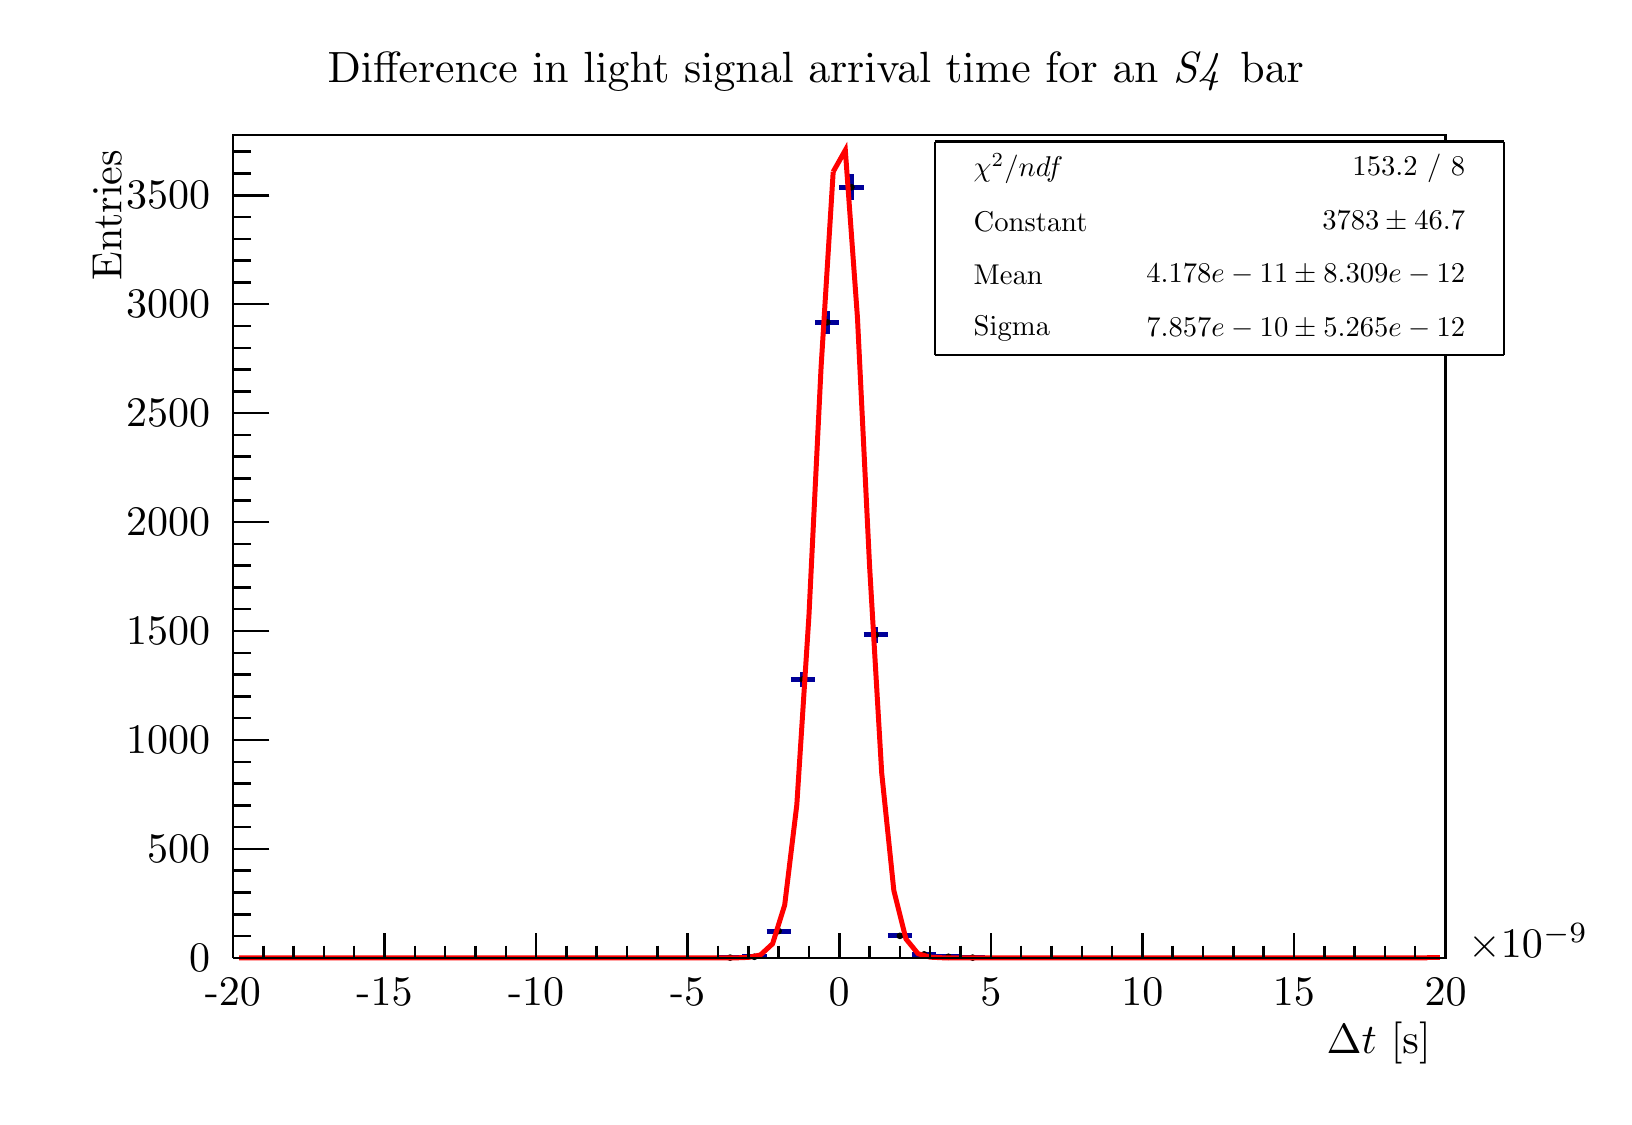
\begin{tikzpicture}
\pgfdeclareplotmark{cross} {
\pgfpathmoveto{\pgfpoint{-0.3\pgfplotmarksize}{\pgfplotmarksize}}
\pgfpathlineto{\pgfpoint{+0.3\pgfplotmarksize}{\pgfplotmarksize}}
\pgfpathlineto{\pgfpoint{+0.3\pgfplotmarksize}{0.3\pgfplotmarksize}}
\pgfpathlineto{\pgfpoint{+1\pgfplotmarksize}{0.3\pgfplotmarksize}}
\pgfpathlineto{\pgfpoint{+1\pgfplotmarksize}{-0.3\pgfplotmarksize}}
\pgfpathlineto{\pgfpoint{+0.3\pgfplotmarksize}{-0.3\pgfplotmarksize}}
\pgfpathlineto{\pgfpoint{+0.3\pgfplotmarksize}{-1.\pgfplotmarksize}}
\pgfpathlineto{\pgfpoint{-0.3\pgfplotmarksize}{-1.\pgfplotmarksize}}
\pgfpathlineto{\pgfpoint{-0.3\pgfplotmarksize}{-0.3\pgfplotmarksize}}
\pgfpathlineto{\pgfpoint{-1.\pgfplotmarksize}{-0.3\pgfplotmarksize}}
\pgfpathlineto{\pgfpoint{-1.\pgfplotmarksize}{0.3\pgfplotmarksize}}
\pgfpathlineto{\pgfpoint{-0.3\pgfplotmarksize}{0.3\pgfplotmarksize}}
\pgfpathclose
\pgfusepathqstroke
}
\pgfdeclareplotmark{cross*} {
\pgfpathmoveto{\pgfpoint{-0.3\pgfplotmarksize}{\pgfplotmarksize}}
\pgfpathlineto{\pgfpoint{+0.3\pgfplotmarksize}{\pgfplotmarksize}}
\pgfpathlineto{\pgfpoint{+0.3\pgfplotmarksize}{0.3\pgfplotmarksize}}
\pgfpathlineto{\pgfpoint{+1\pgfplotmarksize}{0.3\pgfplotmarksize}}
\pgfpathlineto{\pgfpoint{+1\pgfplotmarksize}{-0.3\pgfplotmarksize}}
\pgfpathlineto{\pgfpoint{+0.3\pgfplotmarksize}{-0.3\pgfplotmarksize}}
\pgfpathlineto{\pgfpoint{+0.3\pgfplotmarksize}{-1.\pgfplotmarksize}}
\pgfpathlineto{\pgfpoint{-0.3\pgfplotmarksize}{-1.\pgfplotmarksize}}
\pgfpathlineto{\pgfpoint{-0.3\pgfplotmarksize}{-0.3\pgfplotmarksize}}
\pgfpathlineto{\pgfpoint{-1.\pgfplotmarksize}{-0.3\pgfplotmarksize}}
\pgfpathlineto{\pgfpoint{-1.\pgfplotmarksize}{0.3\pgfplotmarksize}}
\pgfpathlineto{\pgfpoint{-0.3\pgfplotmarksize}{0.3\pgfplotmarksize}}
\pgfpathclose
\pgfusepathqfillstroke
}
\pgfdeclareplotmark{newstar} {
\pgfpathmoveto{\pgfqpoint{0pt}{\pgfplotmarksize}}
\pgfpathlineto{\pgfqpointpolar{44}{0.5\pgfplotmarksize}}
\pgfpathlineto{\pgfqpointpolar{18}{\pgfplotmarksize}}
\pgfpathlineto{\pgfqpointpolar{-20}{0.5\pgfplotmarksize}}
\pgfpathlineto{\pgfqpointpolar{-54}{\pgfplotmarksize}}
\pgfpathlineto{\pgfqpointpolar{-90}{0.5\pgfplotmarksize}}
\pgfpathlineto{\pgfqpointpolar{234}{\pgfplotmarksize}}
\pgfpathlineto{\pgfqpointpolar{198}{0.5\pgfplotmarksize}}
\pgfpathlineto{\pgfqpointpolar{162}{\pgfplotmarksize}}
\pgfpathlineto{\pgfqpointpolar{134}{0.5\pgfplotmarksize}}
\pgfpathclose
\pgfusepathqstroke
}
\pgfdeclareplotmark{newstar*} {
\pgfpathmoveto{\pgfqpoint{0pt}{\pgfplotmarksize}}
\pgfpathlineto{\pgfqpointpolar{44}{0.5\pgfplotmarksize}}
\pgfpathlineto{\pgfqpointpolar{18}{\pgfplotmarksize}}
\pgfpathlineto{\pgfqpointpolar{-20}{0.5\pgfplotmarksize}}
\pgfpathlineto{\pgfqpointpolar{-54}{\pgfplotmarksize}}
\pgfpathlineto{\pgfqpointpolar{-90}{0.5\pgfplotmarksize}}
\pgfpathlineto{\pgfqpointpolar{234}{\pgfplotmarksize}}
\pgfpathlineto{\pgfqpointpolar{198}{0.5\pgfplotmarksize}}
\pgfpathlineto{\pgfqpointpolar{162}{\pgfplotmarksize}}
\pgfpathlineto{\pgfqpointpolar{134}{0.5\pgfplotmarksize}}
\pgfpathclose
\pgfusepathqfillstroke
}
\definecolor{c}{rgb}{1,1,1};
\draw [color=c, fill=c] (0,0) rectangle (20,13.5705);
\draw [color=c, fill=c] (2.6,1.76416) rectangle (18,12.2134);
\definecolor{c}{rgb}{0,0,0};
\draw [c,line width=0.9] (2.6,1.76416) -- (2.6,12.2134) -- (18,12.2134) -- (18,1.76416) -- (2.6,1.76416);
\definecolor{c}{rgb}{1,1,1};
\draw [color=c, fill=c] (2.6,1.76416) rectangle (18,12.2134);
\definecolor{c}{rgb}{0,0,0};
\draw [c,line width=0.9] (2.6,1.76416) -- (2.6,12.2134) -- (18,12.2134) -- (18,1.76416) -- (2.6,1.76416);
\definecolor{c}{rgb}{0,0,0.6};
\draw [c,line width=1.8] (8.914,1.76416) -- (8.914,1.76693);
\draw [c,line width=1.8] (8.914,1.76693) -- (8.914,1.76969);
\draw [c,line width=1.8] (8.76,1.76693) -- (8.914,1.76693);
\draw [c,line width=1.8] (8.914,1.76693) -- (9.068,1.76693);
\definecolor{c}{rgb}{0,0,0};
\foreach \P in {(8.914,1.76693)}{\draw[mark options={color=c,fill=c},mark size=2.402402pt,mark=*,mark size=1pt] plot coordinates {\P};}
\definecolor{c}{rgb}{0,0,0.6};
\draw [c,line width=1.8] (9.222,1.77181) -- (9.222,1.77799);
\draw [c,line width=1.8] (9.222,1.77799) -- (9.222,1.78418);
\draw [c,line width=1.8] (9.068,1.77799) -- (9.222,1.77799);
\draw [c,line width=1.8] (9.222,1.77799) -- (9.376,1.77799);
\definecolor{c}{rgb}{0,0,0};
\foreach \P in {(9.222,1.77799)}{\draw[mark options={color=c,fill=c},mark size=2.402402pt,mark=*,mark size=1pt] plot coordinates {\P};}
\definecolor{c}{rgb}{0,0,0.6};
\draw [c,line width=1.8] (9.53,2.07382) -- (9.53,2.10451);
\draw [c,line width=1.8] (9.53,2.10451) -- (9.53,2.1352);
\draw [c,line width=1.8] (9.376,2.10451) -- (9.53,2.10451);
\draw [c,line width=1.8] (9.53,2.10451) -- (9.684,2.10451);
\definecolor{c}{rgb}{0,0,0};
\foreach \P in {(9.53,2.10451)}{\draw[mark options={color=c,fill=c},mark size=2.402402pt,mark=*,mark size=1pt] plot coordinates {\P};}
\definecolor{c}{rgb}{0,0,0.6};
\draw [c,line width=1.8] (9.838,5.20154) -- (9.838,5.30046);
\draw [c,line width=1.8] (9.838,5.30046) -- (9.838,5.39938);
\draw [c,line width=1.8] (9.684,5.30046) -- (9.838,5.30046);
\draw [c,line width=1.8] (9.838,5.30046) -- (9.992,5.30046);
\definecolor{c}{rgb}{0,0,0};
\foreach \P in {(9.838,5.30046)}{\draw[mark options={color=c,fill=c},mark size=2.402402pt,mark=*,mark size=1pt] plot coordinates {\P};}
\definecolor{c}{rgb}{0,0,0.6};
\draw [c,line width=1.8] (10.146,9.68623) -- (10.146,9.83568);
\draw [c,line width=1.8] (10.146,9.83568) -- (10.146,9.98513);
\draw [c,line width=1.8] (9.992,9.83568) -- (10.146,9.83568);
\draw [c,line width=1.8] (10.146,9.83568) -- (10.3,9.83568);
\definecolor{c}{rgb}{0,0,0};
\foreach \P in {(10.146,9.83568)}{\draw[mark options={color=c,fill=c},mark size=2.402402pt,mark=*,mark size=1pt] plot coordinates {\P};}
\definecolor{c}{rgb}{0,0,0.6};
\draw [c,line width=1.8] (10.454,11.3867) -- (10.454,11.5513);
\draw [c,line width=1.8] (10.454,11.5513) -- (10.454,11.7158);
\draw [c,line width=1.8] (10.3,11.5513) -- (10.454,11.5513);
\draw [c,line width=1.8] (10.454,11.5513) -- (10.608,11.5513);
\definecolor{c}{rgb}{0,0,0};
\foreach \P in {(10.454,11.5513)}{\draw[mark options={color=c,fill=c},mark size=2.402402pt,mark=*,mark size=1pt] plot coordinates {\P};}
\definecolor{c}{rgb}{0,0,0.6};
\draw [c,line width=1.8] (10.762,5.75842) -- (10.762,5.86495);
\draw [c,line width=1.8] (10.762,5.86495) -- (10.762,5.97147);
\draw [c,line width=1.8] (10.608,5.86495) -- (10.762,5.86495);
\draw [c,line width=1.8] (10.762,5.86495) -- (10.916,5.86495);
\definecolor{c}{rgb}{0,0,0};
\foreach \P in {(10.762,5.86495)}{\draw[mark options={color=c,fill=c},mark size=2.402402pt,mark=*,mark size=1pt] plot coordinates {\P};}
\definecolor{c}{rgb}{0,0,0.6};
\draw [c,line width=1.8] (11.07,2.01582) -- (11.07,2.04363);
\draw [c,line width=1.8] (11.07,2.04363) -- (11.07,2.07144);
\draw [c,line width=1.8] (10.916,2.04363) -- (11.07,2.04363);
\draw [c,line width=1.8] (11.07,2.04363) -- (11.224,2.04363);
\definecolor{c}{rgb}{0,0,0};
\foreach \P in {(11.07,2.04363)}{\draw[mark options={color=c,fill=c},mark size=2.402402pt,mark=*,mark size=1pt] plot coordinates {\P};}
\definecolor{c}{rgb}{0,0,0.6};
\draw [c,line width=1.8] (11.378,1.79736) -- (11.378,1.80843);
\draw [c,line width=1.8] (11.378,1.80843) -- (11.378,1.8195);
\draw [c,line width=1.8] (11.224,1.80843) -- (11.378,1.80843);
\draw [c,line width=1.8] (11.378,1.80843) -- (11.532,1.80843);
\definecolor{c}{rgb}{0,0,0};
\foreach \P in {(11.378,1.80843)}{\draw[mark options={color=c,fill=c},mark size=2.402402pt,mark=*,mark size=1pt] plot coordinates {\P};}
\definecolor{c}{rgb}{0,0,0.6};
\draw [c,line width=1.8] (11.686,1.77181) -- (11.686,1.77799);
\draw [c,line width=1.8] (11.686,1.77799) -- (11.686,1.78418);
\draw [c,line width=1.8] (11.532,1.77799) -- (11.686,1.77799);
\draw [c,line width=1.8] (11.686,1.77799) -- (11.84,1.77799);
\definecolor{c}{rgb}{0,0,0};
\foreach \P in {(11.686,1.77799)}{\draw[mark options={color=c,fill=c},mark size=2.402402pt,mark=*,mark size=1pt] plot coordinates {\P};}
\definecolor{c}{rgb}{0,0,0.6};
\draw [c,line width=1.8] (11.994,1.76416) -- (11.994,1.76693);
\draw [c,line width=1.8] (11.994,1.76693) -- (11.994,1.76969);
\draw [c,line width=1.8] (11.84,1.76693) -- (11.994,1.76693);
\draw [c,line width=1.8] (11.994,1.76693) -- (12.148,1.76693);
\definecolor{c}{rgb}{0,0,0};
\foreach \P in {(11.994,1.76693)}{\draw[mark options={color=c,fill=c},mark size=2.402402pt,mark=*,mark size=1pt] plot coordinates {\P};}
\definecolor{c}{rgb}{1,0,0};
\draw [c,line width=1.8] (2.677,1.76416) -- (2.831,1.76416) -- (2.985,1.76416) -- (3.139,1.76416) -- (3.293,1.76416) -- (3.447,1.76416) -- (3.601,1.76416) -- (3.755,1.76416) -- (3.909,1.76416) -- (4.063,1.76416) -- (4.217,1.76416) -- (4.371,1.76416)
 -- (4.525,1.76416) -- (4.679,1.76416) -- (4.833,1.76416) -- (4.987,1.76416) -- (5.141,1.76416) -- (5.295,1.76416) -- (5.449,1.76416) -- (5.603,1.76416) -- (5.757,1.76416) -- (5.911,1.76416) -- (6.065,1.76416) -- (6.219,1.76416) -- (6.373,1.76416) --
 (6.527,1.76416) -- (6.681,1.76416) -- (6.835,1.76416) -- (6.989,1.76416) -- (7.143,1.76416) -- (7.297,1.76416) -- (7.451,1.76416) -- (7.605,1.76416) -- (7.759,1.76416) -- (7.913,1.76416) -- (8.067,1.76416) -- (8.221,1.76416) -- (8.375,1.76416) --
 (8.529,1.76416) -- (8.683,1.76416) -- (8.837,1.76416) -- (8.991,1.76416) -- (9.145,1.76998) -- (9.299,1.80089) -- (9.453,1.94285) -- (9.607,2.43506) -- (9.761,3.70796) -- (9.915,6.11015) -- (10.069,9.26248) -- (10.223,11.7476);
\draw [c,line width=1.8] (10.223,11.7476) -- (10.377,12.0215) -- (10.531,9.89679) -- (10.685,6.74) -- (10.839,4.11347) -- (10.993,2.62012) -- (11.147,2.00482) -- (11.301,1.81637) -- (11.455,1.7729) -- (11.609,1.76529) -- (11.763,1.76416) --
 (11.917,1.76416) -- (12.071,1.76416) -- (12.225,1.76416) -- (12.379,1.76416) -- (12.533,1.76416) -- (12.687,1.76416) -- (12.841,1.76416) -- (12.995,1.76416) -- (13.149,1.76416) -- (13.303,1.76416) -- (13.457,1.76416) -- (13.611,1.76416) --
 (13.765,1.76416) -- (13.919,1.76416) -- (14.073,1.76416) -- (14.227,1.76416) -- (14.381,1.76416) -- (14.535,1.76416) -- (14.689,1.76416) -- (14.843,1.76416) -- (14.997,1.76416) -- (15.151,1.76416) -- (15.305,1.76416) -- (15.459,1.76416) --
 (15.613,1.76416) -- (15.767,1.76416) -- (15.921,1.76416) -- (16.075,1.76416) -- (16.229,1.76416) -- (16.383,1.76416) -- (16.537,1.76416) -- (16.691,1.76416) -- (16.845,1.76416) -- (16.999,1.76416) -- (17.153,1.76416) -- (17.307,1.76416) --
 (17.461,1.76416) -- (17.615,1.76416) -- (17.769,1.76416);
\draw [c,line width=1.8] (17.769,1.76416) -- (17.923,1.76416);
\definecolor{c}{rgb}{1,1,1};
\draw [color=c, fill=c] (11.5186,9.42152) rectangle (18.7393,12.1299);
\definecolor{c}{rgb}{0,0,0};
\draw [c,line width=0.9] (11.5186,9.42152) -- (18.7393,9.42152);
\draw [c,line width=0.9] (18.7393,9.42152) -- (18.7393,12.1299);
\draw [c,line width=0.9] (18.7393,12.1299) -- (11.5186,12.1299);
\draw [c,line width=0.9] (11.5186,12.1299) -- (11.5186,9.42152);
\draw [anchor= west] (11.8797,11.7913) node[scale=1.03301, color=c, rotate=0]{$\chi^{2} / ndf $};
\draw [anchor= east] (18.3782,11.7913) node[scale=1.03301, color=c, rotate=0]{ 153.2 / 8};
\draw [anchor= west] (11.8797,11.1142) node[scale=1.03301, color=c, rotate=0]{Constant };
\draw [anchor= east] (18.3782,11.1142) node[scale=1.03301, color=c, rotate=0]{$  3783 \pm 46.7$};
\draw [anchor= west] (11.8797,10.4371) node[scale=1.03301, color=c, rotate=0]{Mean     };
\draw [anchor= east] (18.3782,10.4371) node[scale=1.03301, color=c, rotate=0]{$ 4.178e-11 \pm 8.309e-12$};
\draw [anchor= west] (11.8797,9.76007) node[scale=1.03301, color=c, rotate=0]{Sigma    };
\draw [anchor= east] (18.3782,9.76007) node[scale=1.03301, color=c, rotate=0]{$ 7.857e-10 \pm 5.265e-12$};
\draw [c,line width=0.9] (2.6,1.76416) -- (18,1.76416);
\draw [c,line width=0.9] (2.6,2.07764) -- (2.6,1.76416);
\draw [c,line width=0.9] (2.985,1.9209) -- (2.985,1.76416);
\draw [c,line width=0.9] (3.37,1.9209) -- (3.37,1.76416);
\draw [c,line width=0.9] (3.755,1.9209) -- (3.755,1.76416);
\draw [c,line width=0.9] (4.14,1.9209) -- (4.14,1.76416);
\draw [c,line width=0.9] (4.525,2.07764) -- (4.525,1.76416);
\draw [c,line width=0.9] (4.91,1.9209) -- (4.91,1.76416);
\draw [c,line width=0.9] (5.295,1.9209) -- (5.295,1.76416);
\draw [c,line width=0.9] (5.68,1.9209) -- (5.68,1.76416);
\draw [c,line width=0.9] (6.065,1.9209) -- (6.065,1.76416);
\draw [c,line width=0.9] (6.45,2.07764) -- (6.45,1.76416);
\draw [c,line width=0.9] (6.835,1.9209) -- (6.835,1.76416);
\draw [c,line width=0.9] (7.22,1.9209) -- (7.22,1.76416);
\draw [c,line width=0.9] (7.605,1.9209) -- (7.605,1.76416);
\draw [c,line width=0.9] (7.99,1.9209) -- (7.99,1.76416);
\draw [c,line width=0.9] (8.375,2.07764) -- (8.375,1.76416);
\draw [c,line width=0.9] (8.76,1.9209) -- (8.76,1.76416);
\draw [c,line width=0.9] (9.145,1.9209) -- (9.145,1.76416);
\draw [c,line width=0.9] (9.53,1.9209) -- (9.53,1.76416);
\draw [c,line width=0.9] (9.915,1.9209) -- (9.915,1.76416);
\draw [c,line width=0.9] (10.3,2.07764) -- (10.3,1.76416);
\draw [c,line width=0.9] (10.685,1.9209) -- (10.685,1.76416);
\draw [c,line width=0.9] (11.07,1.9209) -- (11.07,1.76416);
\draw [c,line width=0.9] (11.455,1.9209) -- (11.455,1.76416);
\draw [c,line width=0.9] (11.84,1.9209) -- (11.84,1.76416);
\draw [c,line width=0.9] (12.225,2.07764) -- (12.225,1.76416);
\draw [c,line width=0.9] (12.61,1.9209) -- (12.61,1.76416);
\draw [c,line width=0.9] (12.995,1.9209) -- (12.995,1.76416);
\draw [c,line width=0.9] (13.38,1.9209) -- (13.38,1.76416);
\draw [c,line width=0.9] (13.765,1.9209) -- (13.765,1.76416);
\draw [c,line width=0.9] (14.15,2.07764) -- (14.15,1.76416);
\draw [c,line width=0.9] (14.535,1.9209) -- (14.535,1.76416);
\draw [c,line width=0.9] (14.92,1.9209) -- (14.92,1.76416);
\draw [c,line width=0.9] (15.305,1.9209) -- (15.305,1.76416);
\draw [c,line width=0.9] (15.69,1.9209) -- (15.69,1.76416);
\draw [c,line width=0.9] (16.075,2.07764) -- (16.075,1.76416);
\draw [c,line width=0.9] (16.46,1.9209) -- (16.46,1.76416);
\draw [c,line width=0.9] (16.845,1.9209) -- (16.845,1.76416);
\draw [c,line width=0.9] (17.23,1.9209) -- (17.23,1.76416);
\draw [c,line width=0.9] (17.615,1.9209) -- (17.615,1.76416);
\draw [c,line width=0.9] (18,2.07764) -- (18,1.76416);
\draw [anchor=base] (2.6,1.15349) node[scale=1.51913, color=c, rotate=0]{-20};
\draw [anchor=base] (4.525,1.15349) node[scale=1.51913, color=c, rotate=0]{-15};
\draw [anchor=base] (6.45,1.15349) node[scale=1.51913, color=c, rotate=0]{-10};
\draw [anchor=base] (8.375,1.15349) node[scale=1.51913, color=c, rotate=0]{-5};
\draw [anchor=base] (10.3,1.15349) node[scale=1.51913, color=c, rotate=0]{0};
\draw [anchor=base] (12.225,1.15349) node[scale=1.51913, color=c, rotate=0]{5};
\draw [anchor=base] (14.15,1.15349) node[scale=1.51913, color=c, rotate=0]{10};
\draw [anchor=base] (16.075,1.15349) node[scale=1.51913, color=c, rotate=0]{15};
\draw [anchor=base] (18,1.15349) node[scale=1.51913, color=c, rotate=0]{20};
\draw [anchor=base west] (18.1,1.76416) node[scale=1.51913, color=c, rotate=0]{$\times10^{-9}$};
\draw [anchor= east] (18,0.678523) node[scale=1.51913, color=c, rotate=0]{$\Delta t$ [s]};
\draw [c,line width=0.9] (2.6,1.76416) -- (2.6,12.2134);
\draw [c,line width=0.9] (3.062,1.76416) -- (2.6,1.76416);
\draw [c,line width=0.9] (2.831,2.04086) -- (2.6,2.04086);
\draw [c,line width=0.9] (2.831,2.31757) -- (2.6,2.31757);
\draw [c,line width=0.9] (2.831,2.59428) -- (2.6,2.59428);
\draw [c,line width=0.9] (2.831,2.87098) -- (2.6,2.87098);
\draw [c,line width=0.9] (3.062,3.14769) -- (2.6,3.14769);
\draw [c,line width=0.9] (2.831,3.4244) -- (2.6,3.4244);
\draw [c,line width=0.9] (2.831,3.7011) -- (2.6,3.7011);
\draw [c,line width=0.9] (2.831,3.97781) -- (2.6,3.97781);
\draw [c,line width=0.9] (2.831,4.25451) -- (2.6,4.25451);
\draw [c,line width=0.9] (3.062,4.53122) -- (2.6,4.53122);
\draw [c,line width=0.9] (2.831,4.80793) -- (2.6,4.80793);
\draw [c,line width=0.9] (2.831,5.08463) -- (2.6,5.08463);
\draw [c,line width=0.9] (2.831,5.36134) -- (2.6,5.36134);
\draw [c,line width=0.9] (2.831,5.63805) -- (2.6,5.63805);
\draw [c,line width=0.9] (3.062,5.91475) -- (2.6,5.91475);
\draw [c,line width=0.9] (2.831,6.19146) -- (2.6,6.19146);
\draw [c,line width=0.9] (2.831,6.46816) -- (2.6,6.46816);
\draw [c,line width=0.9] (2.831,6.74487) -- (2.6,6.74487);
\draw [c,line width=0.9] (2.831,7.02158) -- (2.6,7.02158);
\draw [c,line width=0.9] (3.062,7.29828) -- (2.6,7.29828);
\draw [c,line width=0.9] (2.831,7.57499) -- (2.6,7.57499);
\draw [c,line width=0.9] (2.831,7.8517) -- (2.6,7.8517);
\draw [c,line width=0.9] (2.831,8.1284) -- (2.6,8.1284);
\draw [c,line width=0.9] (2.831,8.40511) -- (2.6,8.40511);
\draw [c,line width=0.9] (3.062,8.68182) -- (2.6,8.68182);
\draw [c,line width=0.9] (2.831,8.95852) -- (2.6,8.95852);
\draw [c,line width=0.9] (2.831,9.23523) -- (2.6,9.23523);
\draw [c,line width=0.9] (2.831,9.51193) -- (2.6,9.51193);
\draw [c,line width=0.9] (2.831,9.78864) -- (2.6,9.78864);
\draw [c,line width=0.9] (3.062,10.0653) -- (2.6,10.0653);
\draw [c,line width=0.9] (2.831,10.3421) -- (2.6,10.3421);
\draw [c,line width=0.9] (2.831,10.6188) -- (2.6,10.6188);
\draw [c,line width=0.9] (2.831,10.8955) -- (2.6,10.8955);
\draw [c,line width=0.9] (2.831,11.1722) -- (2.6,11.1722);
\draw [c,line width=0.9] (3.062,11.4489) -- (2.6,11.4489);
\draw [c,line width=0.9] (3.062,11.4489) -- (2.6,11.4489);
\draw [c,line width=0.9] (2.831,11.7256) -- (2.6,11.7256);
\draw [c,line width=0.9] (2.831,12.0023) -- (2.6,12.0023);
\draw [anchor= east] (2.5,1.76416) node[scale=1.51913, color=c, rotate=0]{0};
\draw [anchor= east] (2.5,3.14769) node[scale=1.51913, color=c, rotate=0]{500};
\draw [anchor= east] (2.5,4.53122) node[scale=1.51913, color=c, rotate=0]{1000};
\draw [anchor= east] (2.5,5.91475) node[scale=1.51913, color=c, rotate=0]{1500};
\draw [anchor= east] (2.5,7.29828) node[scale=1.51913, color=c, rotate=0]{2000};
\draw [anchor= east] (2.5,8.68182) node[scale=1.51913, color=c, rotate=0]{2500};
\draw [anchor= east] (2.5,10.0653) node[scale=1.51913, color=c, rotate=0]{3000};
\draw [anchor= east] (2.5,11.4489) node[scale=1.51913, color=c, rotate=0]{3500};
\draw [anchor= east] (1,12.2134) node[scale=1.51913, color=c, rotate=90]{Entries};
\definecolor{c}{rgb}{1,1,1};
\draw [color=c, fill=c] (11.5186,9.42152) rectangle (18.7393,12.1299);
\definecolor{c}{rgb}{0,0,0};
\draw [c,line width=0.9] (11.5186,9.42152) -- (18.7393,9.42152);
\draw [c,line width=0.9] (18.7393,9.42152) -- (18.7393,12.1299);
\draw [c,line width=0.9] (18.7393,12.1299) -- (11.5186,12.1299);
\draw [c,line width=0.9] (11.5186,12.1299) -- (11.5186,9.42152);
\draw [anchor= west] (11.8797,11.7913) node[scale=1.03301, color=c, rotate=0]{$\chi^{2} / ndf $};
\draw [anchor= east] (18.3782,11.7913) node[scale=1.03301, color=c, rotate=0]{ 153.2 / 8};
\draw [anchor= west] (11.8797,11.1142) node[scale=1.03301, color=c, rotate=0]{Constant };
\draw [anchor= east] (18.3782,11.1142) node[scale=1.03301, color=c, rotate=0]{$  3783 \pm 46.7$};
\draw [anchor= west] (11.8797,10.4371) node[scale=1.03301, color=c, rotate=0]{Mean     };
\draw [anchor= east] (18.3782,10.4371) node[scale=1.03301, color=c, rotate=0]{$ 4.178e-11 \pm 8.309e-12$};
\draw [anchor= west] (11.8797,9.76007) node[scale=1.03301, color=c, rotate=0]{Sigma    };
\draw [anchor= east] (18.3782,9.76007) node[scale=1.03301, color=c, rotate=0]{$ 7.857e-10 \pm 5.265e-12$};
\draw (10,13.0186) node[scale=1.5799, color=c, rotate=0]{Difference in light signal arrival time for an $\mathit{S4}$ bar};
\end{tikzpicture}

	\end{adjustbox}
	\caption{Difference in signal arrival time PMTs at each end of a bar as measured using a $^{90}$Sr source placed 64~cm from one end of the bar.}
	\label{fig:s4Res}	
\end{figure}

\begin{figure}[ht]    
  \centering
  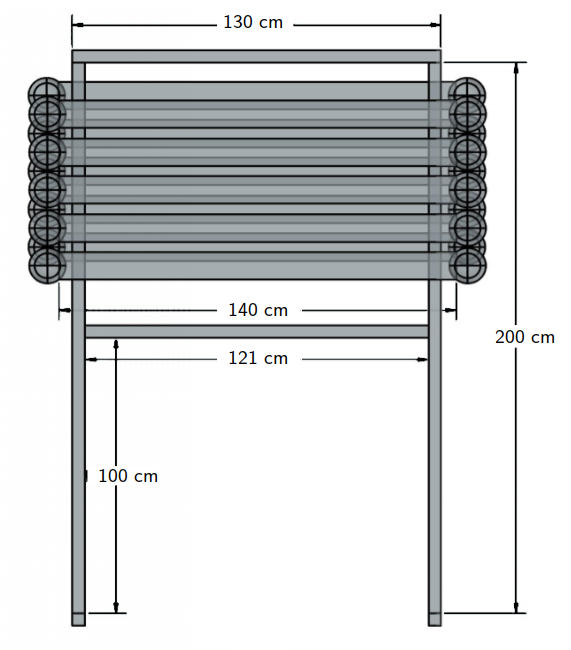
\includegraphics[width=0.5\linewidth]{files/Figures/dstofFront2.png}
  \hfill
  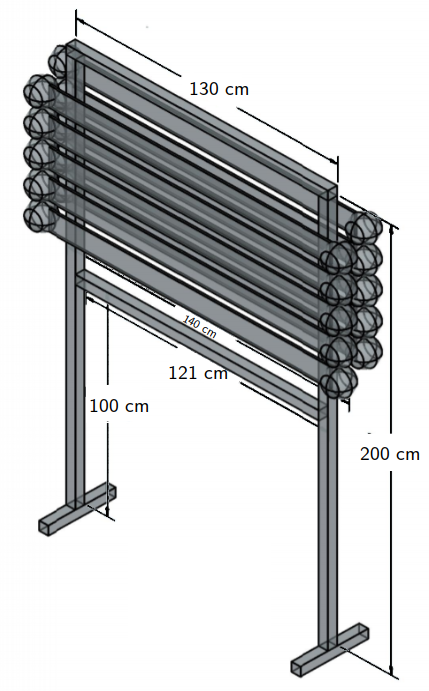
\includegraphics[width=0.35\linewidth]{files/Figures/dstofDiag2.png}
  \caption{Front (left) and rotated (right) view of the $\mathit{S4}$. The rotated view shows more clearly the staggering of the scintillator bars and PMTs.}
  \label{fig:dstofDiagram}
\end{figure}

The anode signals of all 20 of the PMTs are discriminated using LeCroy 620AL NIM discriminators, at a threshold of 20~mV.
The discriminated signals are then fed into a time-to-digital converter. A signal in $\mathit{S4}$ is deemed to have occurred if a signal is seen in both PMTs, above the discriminator threshold, on the same bar within 20~ns of each other. 
This timing window is determined through testing performed with a $^{90}$Sr source at known positions on the bar.

The $\mathit{S1-S2}$ coincidence signal is digitized by the same time-to-digital converter. This signal is used to calculate the particle time of flight from $\mathit{S2}$ to $\mathit{S4}$.

\subsection{The HPTPC Prototype}
\todo[inline]{JOCELYN: This section should given the relevant geometric info on the TPC and how this is known (and how well). It should start with something like ``For the characterisation of the beam using the ToF systems described in this paper, the relevant characteristics of the HPTPC prototype are the location and thickness of the walls''}
The steel vessel is rated to 6~barA of pressure, and the walls of the vessel are 1~cm thick.
The TPC comprised thin steel mesh electrodes (one cathode and three anodes), and 12 copper rings to create the uniform drift field.
\todo[inline]{JOCELYN: Important info which is missing here is the diameter of the field cage and the distance from the inside of the vessel wall to the field cage rings.}
The drift distance produced was 48~cm, with the anodes separated by 1~mm. Data taking with the TPC made use of both optical and charge readout.
The vessel, electrodes, and drift region of the TPC are shown in Figure~\ref{fig:TPC}.

\begin{figure}

  \centering
    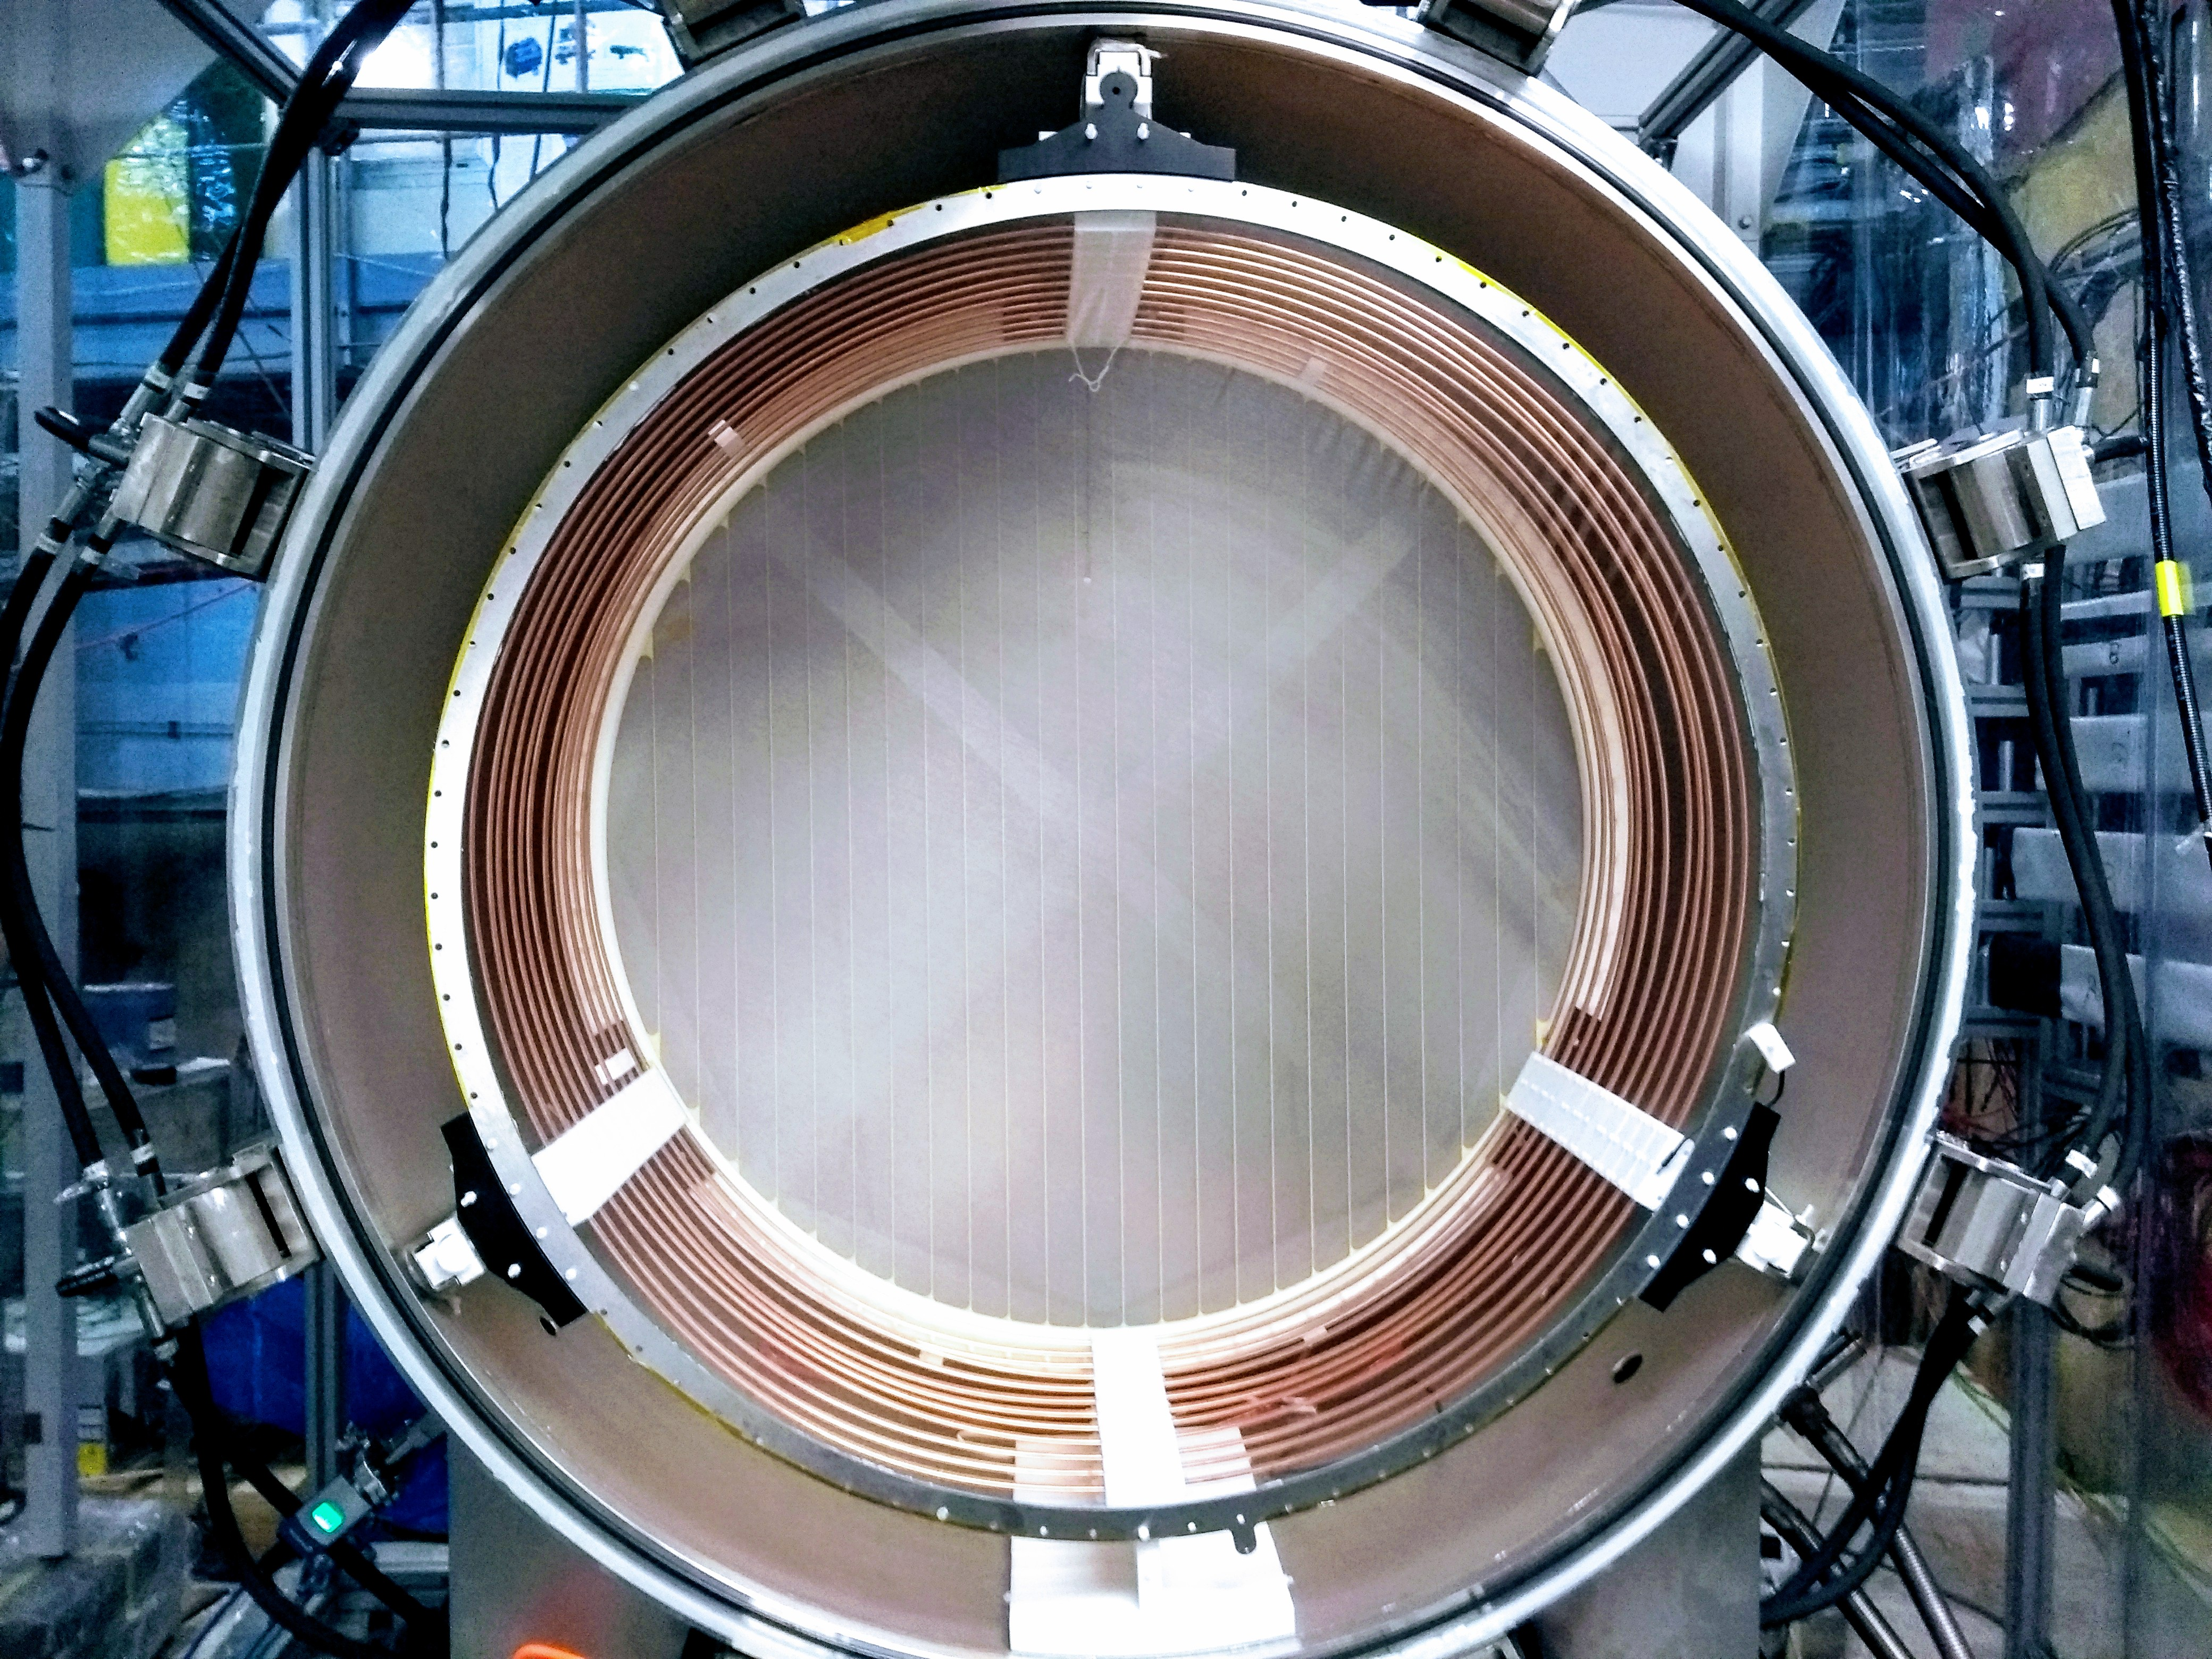
\includegraphics[width=\linewidth]{files/Figures/IMG_20180830_170947192-3.jpg}
  \caption{Cross-sectional view of the TPC; the thin mesh electrodes and copper ring drift volume can be seen inside the steel vessel}
  
   \label{fig:TPC}
   \todo[inline]{TOBY: "This caption needs to give the important quantitative info for the ToF analysis, eg. wall thickness, separation of walls at the height of the beam centre, the distance from the inside of the upstream wall to the drift region, etc"}
   %Vessel: wall thickness 1cm, beam centre height -1.14cm, 
\end{figure}


%The centre of the TPC was placed 13~m from the beam entrance with \textit{S3} and \textit{S4} directly upstream and downstream of the vessel, respectively. 
In the coordinate system shown in Figure~\ref{fig:setup} and detailed in section~\ref{sec:coord}, the TPC centre lies at $X=10.82~\text{m}$, $Y=0.5593~\text{m}$, $Z=-0.0114~\text{m}$. 

Throughout the run, the TPC was filled with either pure argon, or a combination of argon and a small percentage of quencher. 
The performance of this TPC is the subject of a forthcoming publication.

\section{Analysis}
\label{hptpcPaper:sec:Analysis}
\subsection{Analysis Goals}

The primary aims of the use of $\mathit{S1} - \mathit{S4}$ were as follows: to assess the feasibility of using this combination of off-axis positioning and a moderated beam at the PS to produce the momenta of more closely in line with neutrino cross-section studies and to characterize the incident flux on the TPC and exiting the TPC, for the TPC data analysis.

%Protons take longer to travel the distance from \textit{S1} to \textit{S3} or \textit{S4} than lighter particles that are close to being minimum ionising.
%This difference in time of flight can be used to distinguish between the two types of particles.
%Distinguishing these MIPs from one another is more difficult due to their similar masses and can be only determined by the upstream ToF system.
%From the particle flux data, it is possible to measure the ratio of protons to other particles over the range of off-axis angles covered by the \textit{S3} and \textit{S4} walls, and for varying numbers of moderator blocks.

A particle of mass $m$ with momentum $p$ travelling over a distance $d$ will traverse said distance in a time
\begin{align}
	t = d \sqrt{\frac{m^2}{p^2} + \frac{1}{c^2}}
\end{align}
where $c$ is the speed of light in a vacuum.
Therefore, particles with a greater momentum or smaller mass will cross the same distance in a shorter time.
This means that, if there exists a beam of particles of different species but with the same momenta (as is produced by the PS), the mass of of a particle can be determined by measuring this time of flight, $t$.

For example, a charged pion with a momentum of 0.8~GeV/c will have a time of flight from $\mathit{S1}$ to $\mathit{S3}$ (a distance of 10.9~m) of 37~ns, while a proton with the same momentum will have a time of flight of 56~ns.
For the same two particles travelling between $\mathit{S2}$ and $\mathit{S4}$ (a distance of 12.6~m), the charged pion would have a time of flight of 43~ns and the proton would have a time of flight of 65~ns.
\todo[inline]{Add error bars to these numbers.}
Figure~\ref{fig:s1s3PredTimes} and Figure~\ref{fig:s2s4PredTimes} show the predicted time of flight for various particle species across the $\mathit{S1}-\mathit{S3}$ distance and the $\mathit{S2}-\mathit{S4}$ distance respectively.

\begin{figure}[ht]
  \begin{minipage}[t]{0.49\textwidth}
    \begin{adjustbox}{max totalsize={\textwidth}{.5\textheight},center}
      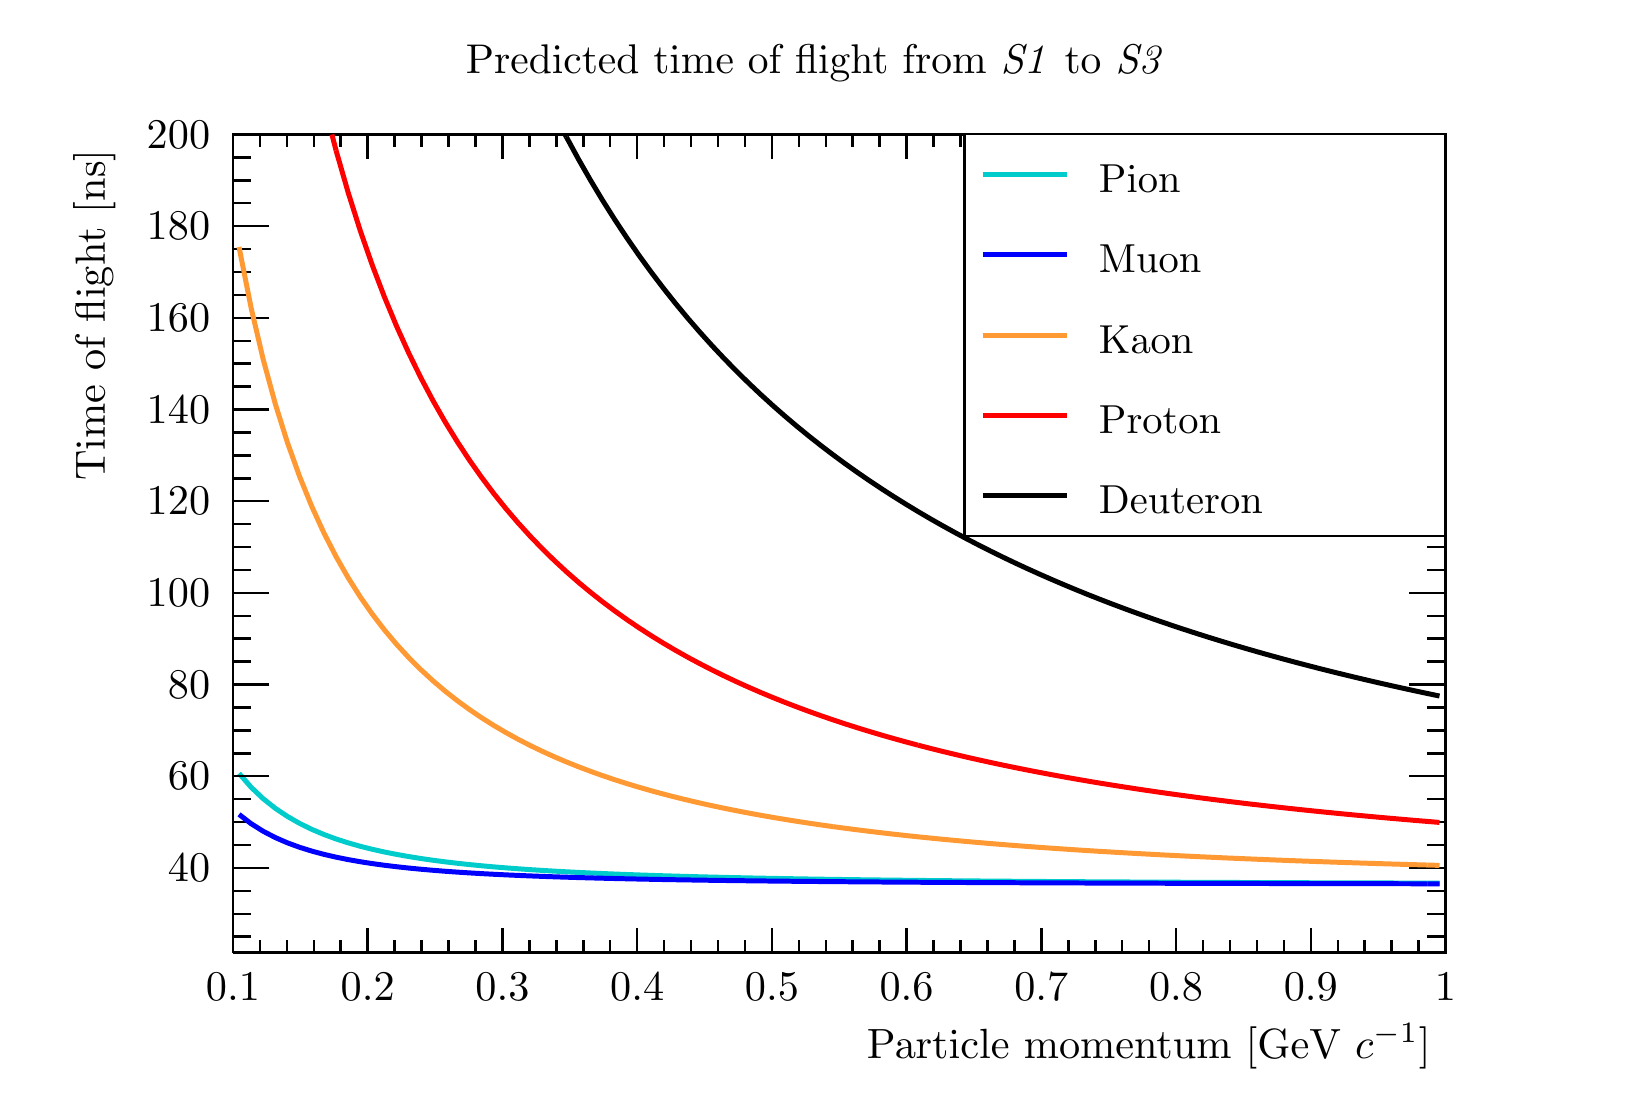
\begin{tikzpicture}
\pgfdeclareplotmark{cross} {
\pgfpathmoveto{\pgfpoint{-0.3\pgfplotmarksize}{\pgfplotmarksize}}
\pgfpathlineto{\pgfpoint{+0.3\pgfplotmarksize}{\pgfplotmarksize}}
\pgfpathlineto{\pgfpoint{+0.3\pgfplotmarksize}{0.3\pgfplotmarksize}}
\pgfpathlineto{\pgfpoint{+1\pgfplotmarksize}{0.3\pgfplotmarksize}}
\pgfpathlineto{\pgfpoint{+1\pgfplotmarksize}{-0.3\pgfplotmarksize}}
\pgfpathlineto{\pgfpoint{+0.3\pgfplotmarksize}{-0.3\pgfplotmarksize}}
\pgfpathlineto{\pgfpoint{+0.3\pgfplotmarksize}{-1.\pgfplotmarksize}}
\pgfpathlineto{\pgfpoint{-0.3\pgfplotmarksize}{-1.\pgfplotmarksize}}
\pgfpathlineto{\pgfpoint{-0.3\pgfplotmarksize}{-0.3\pgfplotmarksize}}
\pgfpathlineto{\pgfpoint{-1.\pgfplotmarksize}{-0.3\pgfplotmarksize}}
\pgfpathlineto{\pgfpoint{-1.\pgfplotmarksize}{0.3\pgfplotmarksize}}
\pgfpathlineto{\pgfpoint{-0.3\pgfplotmarksize}{0.3\pgfplotmarksize}}
\pgfpathclose
\pgfusepathqstroke
}
\pgfdeclareplotmark{cross*} {
\pgfpathmoveto{\pgfpoint{-0.3\pgfplotmarksize}{\pgfplotmarksize}}
\pgfpathlineto{\pgfpoint{+0.3\pgfplotmarksize}{\pgfplotmarksize}}
\pgfpathlineto{\pgfpoint{+0.3\pgfplotmarksize}{0.3\pgfplotmarksize}}
\pgfpathlineto{\pgfpoint{+1\pgfplotmarksize}{0.3\pgfplotmarksize}}
\pgfpathlineto{\pgfpoint{+1\pgfplotmarksize}{-0.3\pgfplotmarksize}}
\pgfpathlineto{\pgfpoint{+0.3\pgfplotmarksize}{-0.3\pgfplotmarksize}}
\pgfpathlineto{\pgfpoint{+0.3\pgfplotmarksize}{-1.\pgfplotmarksize}}
\pgfpathlineto{\pgfpoint{-0.3\pgfplotmarksize}{-1.\pgfplotmarksize}}
\pgfpathlineto{\pgfpoint{-0.3\pgfplotmarksize}{-0.3\pgfplotmarksize}}
\pgfpathlineto{\pgfpoint{-1.\pgfplotmarksize}{-0.3\pgfplotmarksize}}
\pgfpathlineto{\pgfpoint{-1.\pgfplotmarksize}{0.3\pgfplotmarksize}}
\pgfpathlineto{\pgfpoint{-0.3\pgfplotmarksize}{0.3\pgfplotmarksize}}
\pgfpathclose
\pgfusepathqfillstroke
}
\pgfdeclareplotmark{newstar} {
\pgfpathmoveto{\pgfqpoint{0pt}{\pgfplotmarksize}}
\pgfpathlineto{\pgfqpointpolar{44}{0.5\pgfplotmarksize}}
\pgfpathlineto{\pgfqpointpolar{18}{\pgfplotmarksize}}
\pgfpathlineto{\pgfqpointpolar{-20}{0.5\pgfplotmarksize}}
\pgfpathlineto{\pgfqpointpolar{-54}{\pgfplotmarksize}}
\pgfpathlineto{\pgfqpointpolar{-90}{0.5\pgfplotmarksize}}
\pgfpathlineto{\pgfqpointpolar{234}{\pgfplotmarksize}}
\pgfpathlineto{\pgfqpointpolar{198}{0.5\pgfplotmarksize}}
\pgfpathlineto{\pgfqpointpolar{162}{\pgfplotmarksize}}
\pgfpathlineto{\pgfqpointpolar{134}{0.5\pgfplotmarksize}}
\pgfpathclose
\pgfusepathqstroke
}
\pgfdeclareplotmark{newstar*} {
\pgfpathmoveto{\pgfqpoint{0pt}{\pgfplotmarksize}}
\pgfpathlineto{\pgfqpointpolar{44}{0.5\pgfplotmarksize}}
\pgfpathlineto{\pgfqpointpolar{18}{\pgfplotmarksize}}
\pgfpathlineto{\pgfqpointpolar{-20}{0.5\pgfplotmarksize}}
\pgfpathlineto{\pgfqpointpolar{-54}{\pgfplotmarksize}}
\pgfpathlineto{\pgfqpointpolar{-90}{0.5\pgfplotmarksize}}
\pgfpathlineto{\pgfqpointpolar{234}{\pgfplotmarksize}}
\pgfpathlineto{\pgfqpointpolar{198}{0.5\pgfplotmarksize}}
\pgfpathlineto{\pgfqpointpolar{162}{\pgfplotmarksize}}
\pgfpathlineto{\pgfqpointpolar{134}{0.5\pgfplotmarksize}}
\pgfpathclose
\pgfusepathqfillstroke
}
\definecolor{c}{rgb}{1,1,1};
\draw [color=c, fill=c] (0,0) rectangle (20,13.4957);
\draw [color=c, fill=c] (2.6,1.75444) rectangle (18,12.1461);
\definecolor{c}{rgb}{0,0,0};
\draw [c,line width=0.9] (2.6,1.75444) -- (2.6,12.1461) -- (18,12.1461) -- (18,1.75444) -- (2.6,1.75444);
\definecolor{c}{rgb}{1,1,1};
\draw [color=c, fill=c] (2.6,1.75444) rectangle (18,12.1461);
\definecolor{c}{rgb}{0,0,0};
\draw [c,line width=0.9] (2.6,1.75444) -- (2.6,12.1461) -- (18,12.1461) -- (18,1.75444) -- (2.6,1.75444);
\definecolor{c}{rgb}{0,0.8,0.8};
\draw [c,line width=1.8] (2.677,4.03245) -- (2.831,3.85576) -- (2.985,3.70973) -- (3.139,3.58764) -- (3.293,3.48457) -- (3.447,3.39679) -- (3.601,3.32144) -- (3.755,3.2563) -- (3.909,3.19963) -- (4.063,3.15005) -- (4.217,3.10642) -- (4.371,3.06785)
 -- (4.525,3.03359) -- (4.679,3.00304) -- (4.833,2.97568) -- (4.987,2.95108) -- (5.141,2.9289) -- (5.295,2.90884) -- (5.449,2.89062) -- (5.603,2.87404) -- (5.757,2.85891) -- (5.911,2.84507) -- (6.065,2.83237) -- (6.219,2.82069) -- (6.373,2.80993) --
 (6.527,2.8) -- (6.681,2.79081) -- (6.835,2.78229) -- (6.989,2.77438) -- (7.143,2.76702) -- (7.297,2.76017) -- (7.451,2.75377) -- (7.605,2.74779) -- (7.759,2.7422) -- (7.913,2.73696) -- (8.067,2.73203) -- (8.221,2.72741) -- (8.375,2.72306) --
 (8.529,2.71896) -- (8.683,2.7151) -- (8.837,2.71145) -- (8.991,2.708) -- (9.145,2.70474) -- (9.299,2.70165) -- (9.453,2.69873) -- (9.607,2.69595) -- (9.761,2.69331) -- (9.915,2.69081) -- (10.069,2.68842) -- (10.223,2.68615);
\draw [c,line width=1.8] (10.223,2.68615) -- (10.377,2.68399) -- (10.531,2.68193) -- (10.685,2.67997) -- (10.839,2.67809) -- (10.993,2.6763) -- (11.147,2.67458) -- (11.301,2.67294) -- (11.455,2.67137) -- (11.609,2.66986) -- (11.763,2.66842) --
 (11.917,2.66704) -- (12.071,2.66571) -- (12.225,2.66444) -- (12.379,2.66322) -- (12.533,2.66204) -- (12.687,2.66091) -- (12.841,2.65982) -- (12.995,2.65877) -- (13.149,2.65776) -- (13.303,2.65679) -- (13.457,2.65585) -- (13.611,2.65495) --
 (13.765,2.65408) -- (13.919,2.65324) -- (14.073,2.65243) -- (14.227,2.65164) -- (14.381,2.65088) -- (14.535,2.65015) -- (14.689,2.64944) -- (14.843,2.64876) -- (14.997,2.64809) -- (15.151,2.64745) -- (15.305,2.64683) -- (15.459,2.64623) --
 (15.613,2.64564) -- (15.767,2.64508) -- (15.921,2.64453) -- (16.075,2.644) -- (16.229,2.64348) -- (16.383,2.64298) -- (16.537,2.64249) -- (16.691,2.64202) -- (16.845,2.64156) -- (16.999,2.64111) -- (17.153,2.64068) -- (17.307,2.64026) --
 (17.461,2.63985) -- (17.615,2.63945) -- (17.769,2.63906);
\draw [c,line width=1.8] (17.769,2.63906) -- (17.923,2.63869);
\definecolor{c}{rgb}{0,0,0};
\draw [c,line width=0.9] (2.6,1.75444) -- (18,1.75444);
\draw [c,line width=0.9] (2.6,2.06619) -- (2.6,1.75444);
\draw [c,line width=0.9] (2.94222,1.91032) -- (2.94222,1.75444);
\draw [c,line width=0.9] (3.28444,1.91032) -- (3.28444,1.75444);
\draw [c,line width=0.9] (3.62667,1.91032) -- (3.62667,1.75444);
\draw [c,line width=0.9] (3.96889,1.91032) -- (3.96889,1.75444);
\draw [c,line width=0.9] (4.31111,2.06619) -- (4.31111,1.75444);
\draw [c,line width=0.9] (4.65333,1.91032) -- (4.65333,1.75444);
\draw [c,line width=0.9] (4.99556,1.91032) -- (4.99556,1.75444);
\draw [c,line width=0.9] (5.33778,1.91032) -- (5.33778,1.75444);
\draw [c,line width=0.9] (5.68,1.91032) -- (5.68,1.75444);
\draw [c,line width=0.9] (6.02222,2.06619) -- (6.02222,1.75444);
\draw [c,line width=0.9] (6.36444,1.91032) -- (6.36444,1.75444);
\draw [c,line width=0.9] (6.70667,1.91032) -- (6.70667,1.75444);
\draw [c,line width=0.9] (7.04889,1.91032) -- (7.04889,1.75444);
\draw [c,line width=0.9] (7.39111,1.91032) -- (7.39111,1.75444);
\draw [c,line width=0.9] (7.73333,2.06619) -- (7.73333,1.75444);
\draw [c,line width=0.9] (8.07556,1.91032) -- (8.07556,1.75444);
\draw [c,line width=0.9] (8.41778,1.91032) -- (8.41778,1.75444);
\draw [c,line width=0.9] (8.76,1.91032) -- (8.76,1.75444);
\draw [c,line width=0.9] (9.10222,1.91032) -- (9.10222,1.75444);
\draw [c,line width=0.9] (9.44444,2.06619) -- (9.44444,1.75444);
\draw [c,line width=0.9] (9.78667,1.91032) -- (9.78667,1.75444);
\draw [c,line width=0.9] (10.1289,1.91032) -- (10.1289,1.75444);
\draw [c,line width=0.9] (10.4711,1.91032) -- (10.4711,1.75444);
\draw [c,line width=0.9] (10.8133,1.91032) -- (10.8133,1.75444);
\draw [c,line width=0.9] (11.1556,2.06619) -- (11.1556,1.75444);
\draw [c,line width=0.9] (11.4978,1.91032) -- (11.4978,1.75444);
\draw [c,line width=0.9] (11.84,1.91032) -- (11.84,1.75444);
\draw [c,line width=0.9] (12.1822,1.91032) -- (12.1822,1.75444);
\draw [c,line width=0.9] (12.5244,1.91032) -- (12.5244,1.75444);
\draw [c,line width=0.9] (12.8667,2.06619) -- (12.8667,1.75444);
\draw [c,line width=0.9] (13.2089,1.91032) -- (13.2089,1.75444);
\draw [c,line width=0.9] (13.5511,1.91032) -- (13.5511,1.75444);
\draw [c,line width=0.9] (13.8933,1.91032) -- (13.8933,1.75444);
\draw [c,line width=0.9] (14.2356,1.91032) -- (14.2356,1.75444);
\draw [c,line width=0.9] (14.5778,2.06619) -- (14.5778,1.75444);
\draw [c,line width=0.9] (14.92,1.91032) -- (14.92,1.75444);
\draw [c,line width=0.9] (15.2622,1.91032) -- (15.2622,1.75444);
\draw [c,line width=0.9] (15.6044,1.91032) -- (15.6044,1.75444);
\draw [c,line width=0.9] (15.9467,1.91032) -- (15.9467,1.75444);
\draw [c,line width=0.9] (16.2889,2.06619) -- (16.2889,1.75444);
\draw [c,line width=0.9] (16.6311,1.91032) -- (16.6311,1.75444);
\draw [c,line width=0.9] (16.9733,1.91032) -- (16.9733,1.75444);
\draw [c,line width=0.9] (17.3156,1.91032) -- (17.3156,1.75444);
\draw [c,line width=0.9] (17.6578,1.91032) -- (17.6578,1.75444);
\draw [c,line width=0.9] (18,2.06619) -- (18,1.75444);
\draw [anchor=base] (2.6,1.14713) node[scale=1.52731, color=c, rotate=0]{0.1};
\draw [anchor=base] (4.31111,1.14713) node[scale=1.52731, color=c, rotate=0]{0.2};
\draw [anchor=base] (6.02222,1.14713) node[scale=1.52731, color=c, rotate=0]{0.3};
\draw [anchor=base] (7.73333,1.14713) node[scale=1.52731, color=c, rotate=0]{0.4};
\draw [anchor=base] (9.44444,1.14713) node[scale=1.52731, color=c, rotate=0]{0.5};
\draw [anchor=base] (11.1556,1.14713) node[scale=1.52731, color=c, rotate=0]{0.6};
\draw [anchor=base] (12.8667,1.14713) node[scale=1.52731, color=c, rotate=0]{0.7};
\draw [anchor=base] (14.5778,1.14713) node[scale=1.52731, color=c, rotate=0]{0.8};
\draw [anchor=base] (16.2889,1.14713) node[scale=1.52731, color=c, rotate=0]{0.9};
\draw [anchor=base] (18,1.14713) node[scale=1.52731, color=c, rotate=0]{1};
\draw [anchor= east] (18,0.566819) node[scale=1.52731, color=c, rotate=0]{ Particle momentum [GeV $c^{-1}$]};
\draw [c,line width=0.9] (2.6,12.1461) -- (18,12.1461);
\draw [c,line width=0.9] (2.6,11.8344) -- (2.6,12.1461);
\draw [c,line width=0.9] (2.94222,11.9903) -- (2.94222,12.1461);
\draw [c,line width=0.9] (3.28444,11.9903) -- (3.28444,12.1461);
\draw [c,line width=0.9] (3.62667,11.9903) -- (3.62667,12.1461);
\draw [c,line width=0.9] (3.96889,11.9903) -- (3.96889,12.1461);
\draw [c,line width=0.9] (4.31111,11.8344) -- (4.31111,12.1461);
\draw [c,line width=0.9] (4.65333,11.9903) -- (4.65333,12.1461);
\draw [c,line width=0.9] (4.99556,11.9903) -- (4.99556,12.1461);
\draw [c,line width=0.9] (5.33778,11.9903) -- (5.33778,12.1461);
\draw [c,line width=0.9] (5.68,11.9903) -- (5.68,12.1461);
\draw [c,line width=0.9] (6.02222,11.8344) -- (6.02222,12.1461);
\draw [c,line width=0.9] (6.36444,11.9903) -- (6.36444,12.1461);
\draw [c,line width=0.9] (6.70667,11.9903) -- (6.70667,12.1461);
\draw [c,line width=0.9] (7.04889,11.9903) -- (7.04889,12.1461);
\draw [c,line width=0.9] (7.39111,11.9903) -- (7.39111,12.1461);
\draw [c,line width=0.9] (7.73333,11.8344) -- (7.73333,12.1461);
\draw [c,line width=0.9] (8.07556,11.9903) -- (8.07556,12.1461);
\draw [c,line width=0.9] (8.41778,11.9903) -- (8.41778,12.1461);
\draw [c,line width=0.9] (8.76,11.9903) -- (8.76,12.1461);
\draw [c,line width=0.9] (9.10222,11.9903) -- (9.10222,12.1461);
\draw [c,line width=0.9] (9.44444,11.8344) -- (9.44444,12.1461);
\draw [c,line width=0.9] (9.78667,11.9903) -- (9.78667,12.1461);
\draw [c,line width=0.9] (10.1289,11.9903) -- (10.1289,12.1461);
\draw [c,line width=0.9] (10.4711,11.9903) -- (10.4711,12.1461);
\draw [c,line width=0.9] (10.8133,11.9903) -- (10.8133,12.1461);
\draw [c,line width=0.9] (11.1556,11.8344) -- (11.1556,12.1461);
\draw [c,line width=0.9] (11.4978,11.9903) -- (11.4978,12.1461);
\draw [c,line width=0.9] (11.84,11.9903) -- (11.84,12.1461);
\draw [c,line width=0.9] (12.1822,11.9903) -- (12.1822,12.1461);
\draw [c,line width=0.9] (12.5244,11.9903) -- (12.5244,12.1461);
\draw [c,line width=0.9] (12.8667,11.8344) -- (12.8667,12.1461);
\draw [c,line width=0.9] (13.2089,11.9903) -- (13.2089,12.1461);
\draw [c,line width=0.9] (13.5511,11.9903) -- (13.5511,12.1461);
\draw [c,line width=0.9] (13.8933,11.9903) -- (13.8933,12.1461);
\draw [c,line width=0.9] (14.2356,11.9903) -- (14.2356,12.1461);
\draw [c,line width=0.9] (14.5778,11.8344) -- (14.5778,12.1461);
\draw [c,line width=0.9] (14.92,11.9903) -- (14.92,12.1461);
\draw [c,line width=0.9] (15.2622,11.9903) -- (15.2622,12.1461);
\draw [c,line width=0.9] (15.6044,11.9903) -- (15.6044,12.1461);
\draw [c,line width=0.9] (15.9467,11.9903) -- (15.9467,12.1461);
\draw [c,line width=0.9] (16.2889,11.8344) -- (16.2889,12.1461);
\draw [c,line width=0.9] (16.6311,11.9903) -- (16.6311,12.1461);
\draw [c,line width=0.9] (16.9733,11.9903) -- (16.9733,12.1461);
\draw [c,line width=0.9] (17.3156,11.9903) -- (17.3156,12.1461);
\draw [c,line width=0.9] (17.6578,11.9903) -- (17.6578,12.1461);
\draw [c,line width=0.9] (18,11.8344) -- (18,12.1461);
\draw [c,line width=0.9] (2.6,1.75444) -- (2.6,12.1461);
\draw [c,line width=0.9] (3.062,2.83145) -- (2.6,2.83145);
\draw [c,line width=0.9] (2.831,3.12253) -- (2.6,3.12253);
\draw [c,line width=0.9] (2.831,3.41362) -- (2.6,3.41362);
\draw [c,line width=0.9] (2.831,3.7047) -- (2.6,3.7047);
\draw [c,line width=0.9] (3.062,3.99579) -- (2.6,3.99579);
\draw [c,line width=0.9] (2.831,4.28687) -- (2.6,4.28687);
\draw [c,line width=0.9] (2.831,4.57795) -- (2.6,4.57795);
\draw [c,line width=0.9] (2.831,4.86904) -- (2.6,4.86904);
\draw [c,line width=0.9] (3.062,5.16012) -- (2.6,5.16012);
\draw [c,line width=0.9] (2.831,5.4512) -- (2.6,5.4512);
\draw [c,line width=0.9] (2.831,5.74229) -- (2.6,5.74229);
\draw [c,line width=0.9] (2.831,6.03337) -- (2.6,6.03337);
\draw [c,line width=0.9] (3.062,6.32446) -- (2.6,6.32446);
\draw [c,line width=0.9] (2.831,6.61554) -- (2.6,6.61554);
\draw [c,line width=0.9] (2.831,6.90662) -- (2.6,6.90662);
\draw [c,line width=0.9] (2.831,7.19771) -- (2.6,7.19771);
\draw [c,line width=0.9] (3.062,7.48879) -- (2.6,7.48879);
\draw [c,line width=0.9] (2.831,7.77988) -- (2.6,7.77988);
\draw [c,line width=0.9] (2.831,8.07096) -- (2.6,8.07096);
\draw [c,line width=0.9] (2.831,8.36204) -- (2.6,8.36204);
\draw [c,line width=0.9] (3.062,8.65313) -- (2.6,8.65313);
\draw [c,line width=0.9] (2.831,8.94421) -- (2.6,8.94421);
\draw [c,line width=0.9] (2.831,9.23529) -- (2.6,9.23529);
\draw [c,line width=0.9] (2.831,9.52638) -- (2.6,9.52638);
\draw [c,line width=0.9] (3.062,9.81746) -- (2.6,9.81746);
\draw [c,line width=0.9] (2.831,10.1085) -- (2.6,10.1085);
\draw [c,line width=0.9] (2.831,10.3996) -- (2.6,10.3996);
\draw [c,line width=0.9] (2.831,10.6907) -- (2.6,10.6907);
\draw [c,line width=0.9] (3.062,10.9818) -- (2.6,10.9818);
\draw [c,line width=0.9] (2.831,11.2729) -- (2.6,11.2729);
\draw [c,line width=0.9] (2.831,11.564) -- (2.6,11.564);
\draw [c,line width=0.9] (2.831,11.855) -- (2.6,11.855);
\draw [c,line width=0.9] (3.062,12.1461) -- (2.6,12.1461);
\draw [c,line width=0.9] (3.062,2.83145) -- (2.6,2.83145);
\draw [c,line width=0.9] (2.831,2.54037) -- (2.6,2.54037);
\draw [c,line width=0.9] (2.831,2.24928) -- (2.6,2.24928);
\draw [c,line width=0.9] (2.831,1.9582) -- (2.6,1.9582);
\draw [anchor= east] (2.5,2.83145) node[scale=1.52731, color=c, rotate=0]{40};
\draw [anchor= east] (2.5,3.99579) node[scale=1.52731, color=c, rotate=0]{60};
\draw [anchor= east] (2.5,5.16012) node[scale=1.52731, color=c, rotate=0]{80};
\draw [anchor= east] (2.5,6.32446) node[scale=1.52731, color=c, rotate=0]{100};
\draw [anchor= east] (2.5,7.48879) node[scale=1.52731, color=c, rotate=0]{120};
\draw [anchor= east] (2.5,8.65313) node[scale=1.52731, color=c, rotate=0]{140};
\draw [anchor= east] (2.5,9.81746) node[scale=1.52731, color=c, rotate=0]{160};
\draw [anchor= east] (2.5,10.9818) node[scale=1.52731, color=c, rotate=0]{180};
\draw [anchor= east] (2.5,12.1461) node[scale=1.52731, color=c, rotate=0]{200};
\draw [anchor= east] (0.84,12.1461) node[scale=1.52731, color=c, rotate=90]{ Time of flight [ns]};
\draw [c,line width=0.9] (18,1.75444) -- (18,12.1461);
\draw [c,line width=0.9] (17.538,2.83145) -- (18,2.83145);
\draw [c,line width=0.9] (17.769,3.12253) -- (18,3.12253);
\draw [c,line width=0.9] (17.769,3.41362) -- (18,3.41362);
\draw [c,line width=0.9] (17.769,3.7047) -- (18,3.7047);
\draw [c,line width=0.9] (17.538,3.99579) -- (18,3.99579);
\draw [c,line width=0.9] (17.769,4.28687) -- (18,4.28687);
\draw [c,line width=0.9] (17.769,4.57795) -- (18,4.57795);
\draw [c,line width=0.9] (17.769,4.86904) -- (18,4.86904);
\draw [c,line width=0.9] (17.538,5.16012) -- (18,5.16012);
\draw [c,line width=0.9] (17.769,5.4512) -- (18,5.4512);
\draw [c,line width=0.9] (17.769,5.74229) -- (18,5.74229);
\draw [c,line width=0.9] (17.769,6.03337) -- (18,6.03337);
\draw [c,line width=0.9] (17.538,6.32446) -- (18,6.32446);
\draw [c,line width=0.9] (17.769,6.61554) -- (18,6.61554);
\draw [c,line width=0.9] (17.769,6.90662) -- (18,6.90662);
\draw [c,line width=0.9] (17.769,7.19771) -- (18,7.19771);
\draw [c,line width=0.9] (17.538,7.48879) -- (18,7.48879);
\draw [c,line width=0.9] (17.769,7.77988) -- (18,7.77988);
\draw [c,line width=0.9] (17.769,8.07096) -- (18,8.07096);
\draw [c,line width=0.9] (17.769,8.36204) -- (18,8.36204);
\draw [c,line width=0.9] (17.538,8.65313) -- (18,8.65313);
\draw [c,line width=0.9] (17.769,8.94421) -- (18,8.94421);
\draw [c,line width=0.9] (17.769,9.23529) -- (18,9.23529);
\draw [c,line width=0.9] (17.769,9.52638) -- (18,9.52638);
\draw [c,line width=0.9] (17.538,9.81746) -- (18,9.81746);
\draw [c,line width=0.9] (17.769,10.1085) -- (18,10.1085);
\draw [c,line width=0.9] (17.769,10.3996) -- (18,10.3996);
\draw [c,line width=0.9] (17.769,10.6907) -- (18,10.6907);
\draw [c,line width=0.9] (17.538,10.9818) -- (18,10.9818);
\draw [c,line width=0.9] (17.769,11.2729) -- (18,11.2729);
\draw [c,line width=0.9] (17.769,11.564) -- (18,11.564);
\draw [c,line width=0.9] (17.769,11.855) -- (18,11.855);
\draw [c,line width=0.9] (17.538,12.1461) -- (18,12.1461);
\draw [c,line width=0.9] (17.538,2.83145) -- (18,2.83145);
\draw [c,line width=0.9] (17.769,2.54037) -- (18,2.54037);
\draw [c,line width=0.9] (17.769,2.24928) -- (18,2.24928);
\draw [c,line width=0.9] (17.769,1.9582) -- (18,1.9582);
\definecolor{c}{rgb}{1,0,0};
\draw [c,line width=1.8] (3.85682,12.1461) -- (3.909,11.9448);
\draw [c,line width=1.8] (3.909,11.9448) -- (4.063,11.4091) -- (4.217,10.9238) -- (4.371,10.4823) -- (4.525,10.0791) -- (4.679,9.70933) -- (4.833,9.3692) -- (4.987,9.05532) -- (5.141,8.76485) -- (5.295,8.49533) -- (5.449,8.24462) -- (5.603,8.01089)
 -- (5.757,7.7925) -- (5.911,7.58806) -- (6.065,7.39631) -- (6.219,7.21614) -- (6.373,7.04658) -- (6.527,6.88675) -- (6.681,6.73588) -- (6.835,6.59325) -- (6.989,6.45825) -- (7.143,6.33031) -- (7.297,6.20891) -- (7.451,6.09359) -- (7.605,5.98392) --
 (7.759,5.87953) -- (7.913,5.78007) -- (8.067,5.6852) -- (8.221,5.59465) -- (8.375,5.50813) -- (8.529,5.42541) -- (8.683,5.34625) -- (8.837,5.27045) -- (8.991,5.1978) -- (9.145,5.12814) -- (9.299,5.06128) -- (9.453,4.99709) -- (9.607,4.93541) --
 (9.761,4.8761) -- (9.915,4.81906) -- (10.069,4.76415) -- (10.223,4.71128) -- (10.377,4.66033) -- (10.531,4.61122) -- (10.685,4.56385) -- (10.839,4.51815) -- (10.993,4.47402) -- (11.147,4.43141) -- (11.301,4.39024);
\draw [c,line width=1.8] (11.301,4.39024) -- (11.455,4.35044) -- (11.609,4.31196) -- (11.763,4.27473) -- (11.917,4.2387) -- (12.071,4.20382) -- (12.225,4.17004) -- (12.379,4.13731) -- (12.533,4.1056) -- (12.687,4.07485) -- (12.841,4.04503) --
 (12.995,4.0161) -- (13.149,3.98803) -- (13.303,3.96078) -- (13.457,3.93433) -- (13.611,3.90863) -- (13.765,3.88367) -- (13.919,3.85941) -- (14.073,3.83582) -- (14.227,3.81289) -- (14.381,3.79059) -- (14.535,3.76889) -- (14.689,3.74778) --
 (14.843,3.72724) -- (14.997,3.70723) -- (15.151,3.68775) -- (15.305,3.66878) -- (15.459,3.6503) -- (15.613,3.63229) -- (15.767,3.61474) -- (15.921,3.59762) -- (16.075,3.58094) -- (16.229,3.56467) -- (16.383,3.5488) -- (16.537,3.53331) --
 (16.691,3.5182) -- (16.845,3.50346) -- (16.999,3.48906) -- (17.153,3.475) -- (17.307,3.46128) -- (17.461,3.44787) -- (17.615,3.43477) -- (17.769,3.42197) -- (17.923,3.40947);
\definecolor{c}{rgb}{0,0,1};
\draw [c,line width=1.8] (2.677,3.51136) -- (2.831,3.39318) -- (2.985,3.29656) -- (3.139,3.2166) -- (3.293,3.14973) -- (3.447,3.09327) -- (3.601,3.04519) -- (3.755,3.00394) -- (3.909,2.96828) -- (4.063,2.93728) -- (4.217,2.91016) -- (4.371,2.8863) --
 (4.525,2.86521) -- (4.679,2.84649) -- (4.833,2.82978) -- (4.987,2.81483) -- (5.141,2.80139) -- (5.295,2.78926) -- (5.449,2.77829) -- (5.603,2.76833) -- (5.757,2.75926) -- (5.911,2.75098) -- (6.065,2.7434) -- (6.219,2.73645) -- (6.373,2.73005) --
 (6.527,2.72416) -- (6.681,2.71871) -- (6.835,2.71368) -- (6.989,2.709) -- (7.143,2.70466) -- (7.297,2.70063) -- (7.451,2.69686) -- (7.605,2.69335) -- (7.759,2.69006) -- (7.913,2.68699) -- (8.067,2.6841) -- (8.221,2.68139) -- (8.375,2.67885) --
 (8.529,2.67645) -- (8.683,2.67419) -- (8.837,2.67206) -- (8.991,2.67005) -- (9.145,2.66815) -- (9.299,2.66635) -- (9.453,2.66464) -- (9.607,2.66303) -- (9.761,2.66149) -- (9.915,2.66004) -- (10.069,2.65865) -- (10.223,2.65733);
\draw [c,line width=1.8] (10.223,2.65733) -- (10.377,2.65608) -- (10.531,2.65488) -- (10.685,2.65374) -- (10.839,2.65265) -- (10.993,2.65161) -- (11.147,2.65062) -- (11.301,2.64966) -- (11.455,2.64875) -- (11.609,2.64788) -- (11.763,2.64705) --
 (11.917,2.64625) -- (12.071,2.64548) -- (12.225,2.64474) -- (12.379,2.64403) -- (12.533,2.64335) -- (12.687,2.6427) -- (12.841,2.64207) -- (12.995,2.64147) -- (13.149,2.64088) -- (13.303,2.64032) -- (13.457,2.63978) -- (13.611,2.63926) --
 (13.765,2.63875) -- (13.919,2.63827) -- (14.073,2.6378) -- (14.227,2.63735) -- (14.381,2.63691) -- (14.535,2.63649) -- (14.689,2.63608) -- (14.843,2.63568) -- (14.997,2.6353) -- (15.151,2.63493) -- (15.305,2.63457) -- (15.459,2.63422) --
 (15.613,2.63389) -- (15.767,2.63356) -- (15.921,2.63325) -- (16.075,2.63294) -- (16.229,2.63264) -- (16.383,2.63235) -- (16.537,2.63207) -- (16.691,2.6318) -- (16.845,2.63154) -- (16.999,2.63128) -- (17.153,2.63103) -- (17.307,2.63079) --
 (17.461,2.63055) -- (17.615,2.63032) -- (17.769,2.6301);
\draw [c,line width=1.8] (17.769,2.6301) -- (17.923,2.62988);
\definecolor{c}{rgb}{1,0.6,0.2};
\draw [c,line width=1.8] (2.677,10.7173) -- (2.831,9.94348) -- (2.985,9.286) -- (3.139,8.72093) -- (3.293,8.23049) -- (3.447,7.80116) -- (3.601,7.4225) -- (3.755,7.08633) -- (3.909,6.78611) -- (4.063,6.51658) -- (4.217,6.27346) -- (4.371,6.05322) --
 (4.525,5.85292) -- (4.679,5.67011) -- (4.833,5.50273) -- (4.987,5.349) -- (5.141,5.20742) -- (5.295,5.07671) -- (5.449,4.95572) -- (5.603,4.8435) -- (5.757,4.7392) -- (5.911,4.64206) -- (6.065,4.55142) -- (6.219,4.46672) -- (6.373,4.38743) --
 (6.527,4.31309) -- (6.681,4.24329) -- (6.835,4.17767) -- (6.989,4.1159) -- (7.143,4.05767) -- (7.297,4.00273) -- (7.451,3.95082) -- (7.605,3.90172) -- (7.759,3.85524) -- (7.913,3.8112) -- (8.067,3.76942) -- (8.221,3.72975) -- (8.375,3.69206) --
 (8.529,3.65621) -- (8.683,3.62209) -- (8.837,3.58959) -- (8.991,3.55861) -- (9.145,3.52906) -- (9.299,3.50084) -- (9.453,3.47389) -- (9.607,3.44812) -- (9.761,3.42348) -- (9.915,3.39989) -- (10.069,3.3773) -- (10.223,3.35565);
\draw [c,line width=1.8] (10.223,3.35565) -- (10.377,3.33489) -- (10.531,3.31498) -- (10.685,3.29587) -- (10.839,3.27751) -- (10.993,3.25988) -- (11.147,3.24292) -- (11.301,3.22662) -- (11.455,3.21093) -- (11.609,3.19582) -- (11.763,3.18128) --
 (11.917,3.16726) -- (12.071,3.15375) -- (12.225,3.14072) -- (12.379,3.12815) -- (12.533,3.11602) -- (12.687,3.10431) -- (12.841,3.093) -- (12.995,3.08207) -- (13.149,3.0715) -- (13.303,3.06129) -- (13.457,3.05141) -- (13.611,3.04185) --
 (13.765,3.03259) -- (13.919,3.02363) -- (14.073,3.01495) -- (14.227,3.00655) -- (14.381,2.9984) -- (14.535,2.9905) -- (14.689,2.98284) -- (14.843,2.97541) -- (14.997,2.9682) -- (15.151,2.9612) -- (15.305,2.95441) -- (15.459,2.94781) --
 (15.613,2.9414) -- (15.767,2.93517) -- (15.921,2.92912) -- (16.075,2.92324) -- (16.229,2.91752) -- (16.383,2.91196) -- (16.537,2.90654) -- (16.691,2.90128) -- (16.845,2.89615) -- (16.999,2.89116) -- (17.153,2.8863) -- (17.307,2.88157) --
 (17.461,2.87696) -- (17.615,2.87247) -- (17.769,2.86809);
\draw [c,line width=1.8] (17.769,2.86809) -- (17.923,2.86382);
\definecolor{c}{rgb}{0,0,0};
\draw [c,line width=1.8] (6.81829,12.1461) -- (6.835,12.1137);
\draw [c,line width=1.8] (6.835,12.1137) -- (6.989,11.8304) -- (7.143,11.5614) -- (7.297,11.3054) -- (7.451,11.0618) -- (7.605,10.8295) -- (7.759,10.6078) -- (7.913,10.3961) -- (8.067,10.1936) -- (8.221,9.99987) -- (8.375,9.81429) -- (8.529,9.63638)
 -- (8.683,9.46568) -- (8.837,9.30178) -- (8.991,9.14429) -- (9.145,8.99285) -- (9.299,8.84712) -- (9.453,8.70679) -- (9.607,8.57159) -- (9.761,8.44124) -- (9.915,8.31549) -- (10.069,8.19411) -- (10.223,8.07688) -- (10.377,7.96361) -- (10.531,7.8541)
 -- (10.685,7.74817) -- (10.839,7.64566) -- (10.993,7.5464) -- (11.147,7.45026) -- (11.301,7.3571) -- (11.455,7.26677) -- (11.609,7.17917) -- (11.763,7.09417) -- (11.917,7.01166) -- (12.071,6.93155) -- (12.225,6.85373) -- (12.379,6.7781) --
 (12.533,6.7046) -- (12.687,6.63312) -- (12.841,6.56358) -- (12.995,6.49593) -- (13.149,6.43008) -- (13.303,6.36596) -- (13.457,6.30352) -- (13.611,6.24269) -- (13.765,6.18341) -- (13.919,6.12563) -- (14.073,6.06929) -- (14.227,6.01435);
\draw [c,line width=1.8] (14.227,6.01435) -- (14.381,5.96075) -- (14.535,5.90845) -- (14.689,5.85741) -- (14.843,5.80758) -- (14.997,5.75892) -- (15.151,5.7114) -- (15.305,5.66498) -- (15.459,5.61962) -- (15.613,5.57528) -- (15.767,5.53195) --
 (15.921,5.48958) -- (16.075,5.44814) -- (16.229,5.40762) -- (16.383,5.36797) -- (16.537,5.32918) -- (16.691,5.29121) -- (16.845,5.25405) -- (16.999,5.21767) -- (17.153,5.18204) -- (17.307,5.14715) -- (17.461,5.11298) -- (17.615,5.0795) --
 (17.769,5.0467) -- (17.923,5.01455);
\definecolor{c}{rgb}{1,1,1};
\draw [color=c, fill=c] (11.8911,7.04871) rectangle (17.9943,12.149);
\definecolor{c}{rgb}{0,0,0};
\draw [c,line width=0.9] (11.8911,7.04871) -- (17.9943,7.04871);
\draw [c,line width=0.9] (17.9943,7.04871) -- (17.9943,12.149);
\draw [c,line width=0.9] (17.9943,12.149) -- (11.8911,12.149);
\draw [c,line width=0.9] (11.8911,12.149) -- (11.8911,7.04871);
\draw [anchor=base west] (13.4169,11.4095) node[scale=1.46368, color=c, rotate=0]{Pion};
\definecolor{c}{rgb}{0,0.8,0.8};
\draw [c,line width=1.8] (12.12,11.639) -- (13.188,11.639);
\definecolor{c}{rgb}{0,0,0};
\draw [anchor=base west] (13.4169,10.3894) node[scale=1.46368, color=c, rotate=0]{Muon};
\definecolor{c}{rgb}{0,0,1};
\draw [c,line width=1.8] (12.12,10.6189) -- (13.188,10.6189);
\definecolor{c}{rgb}{0,0,0};
\draw [anchor=base west] (13.4169,9.36934) node[scale=1.46368, color=c, rotate=0]{Kaon};
\definecolor{c}{rgb}{1,0.6,0.2};
\draw [c,line width=1.8] (12.12,9.59885) -- (13.188,9.59885);
\definecolor{c}{rgb}{0,0,0};
\draw [anchor=base west] (13.4169,8.34928) node[scale=1.46368, color=c, rotate=0]{Proton};
\definecolor{c}{rgb}{1,0,0};
\draw [c,line width=1.8] (12.12,8.5788) -- (13.188,8.5788);
\definecolor{c}{rgb}{0,0,0};
\draw [anchor=base west] (13.4169,7.32923) node[scale=1.46368, color=c, rotate=0]{Deuteron};
\draw [c,line width=1.8] (12.12,7.55874) -- (13.188,7.55874);
\definecolor{c}{rgb}{1,1,1};
\draw [color=c, fill=c] (2,12.686) rectangle (18,13.4282);
\definecolor{c}{rgb}{0,0,0};
\draw (10,13.0571) node[scale=1.50004, color=c, rotate=0]{Predicted time of flight from $\mathit{S1}$ to $\mathit{S3}$};
\end{tikzpicture}

    \end{adjustbox}
    \caption{Calculated time of flight between $\mathit{S1}$ and $\mathit{S3}$ for a number of different particle species at different particle momenta.}
    \label{fig:s1s3PredTimes}
  \end{minipage}
  \hfill
  \begin{minipage}[t]{0.49\textwidth}
    \begin{adjustbox}{max totalsize={\textwidth}{.5\textheight},center}
      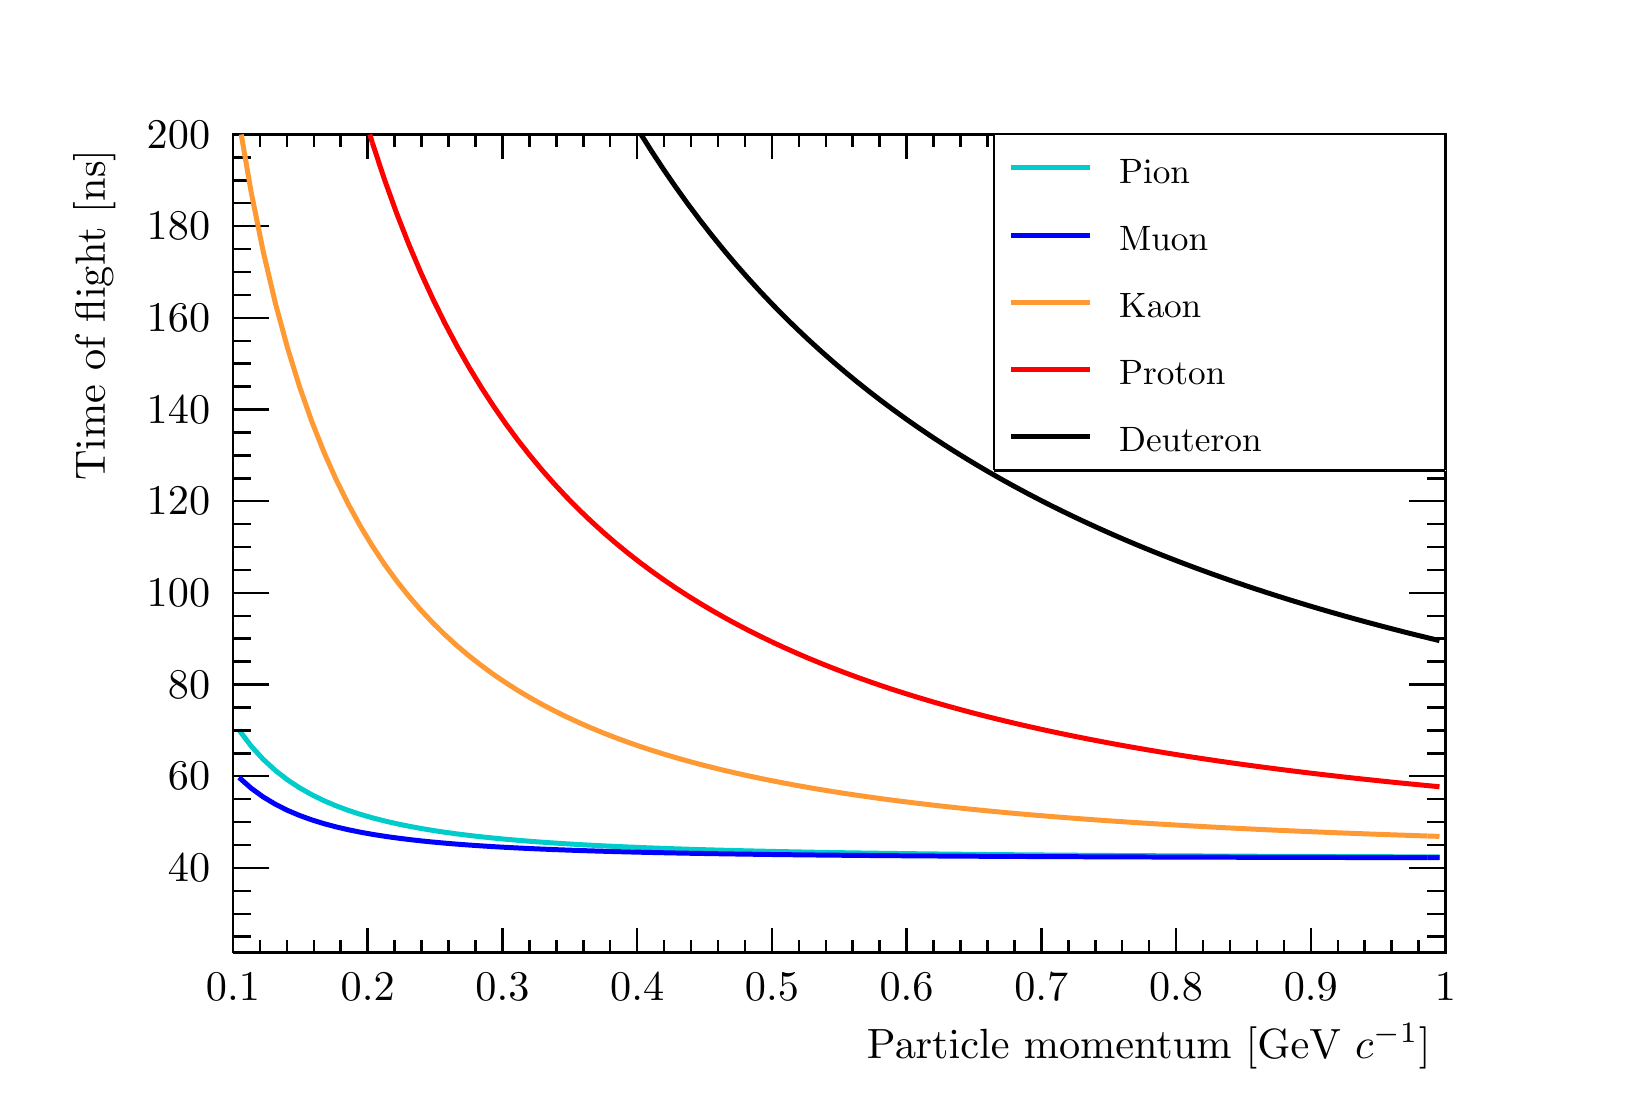
\begin{tikzpicture}
\pgfdeclareplotmark{cross} {
\pgfpathmoveto{\pgfpoint{-0.3\pgfplotmarksize}{\pgfplotmarksize}}
\pgfpathlineto{\pgfpoint{+0.3\pgfplotmarksize}{\pgfplotmarksize}}
\pgfpathlineto{\pgfpoint{+0.3\pgfplotmarksize}{0.3\pgfplotmarksize}}
\pgfpathlineto{\pgfpoint{+1\pgfplotmarksize}{0.3\pgfplotmarksize}}
\pgfpathlineto{\pgfpoint{+1\pgfplotmarksize}{-0.3\pgfplotmarksize}}
\pgfpathlineto{\pgfpoint{+0.3\pgfplotmarksize}{-0.3\pgfplotmarksize}}
\pgfpathlineto{\pgfpoint{+0.3\pgfplotmarksize}{-1.\pgfplotmarksize}}
\pgfpathlineto{\pgfpoint{-0.3\pgfplotmarksize}{-1.\pgfplotmarksize}}
\pgfpathlineto{\pgfpoint{-0.3\pgfplotmarksize}{-0.3\pgfplotmarksize}}
\pgfpathlineto{\pgfpoint{-1.\pgfplotmarksize}{-0.3\pgfplotmarksize}}
\pgfpathlineto{\pgfpoint{-1.\pgfplotmarksize}{0.3\pgfplotmarksize}}
\pgfpathlineto{\pgfpoint{-0.3\pgfplotmarksize}{0.3\pgfplotmarksize}}
\pgfpathclose
\pgfusepathqstroke
}
\pgfdeclareplotmark{cross*} {
\pgfpathmoveto{\pgfpoint{-0.3\pgfplotmarksize}{\pgfplotmarksize}}
\pgfpathlineto{\pgfpoint{+0.3\pgfplotmarksize}{\pgfplotmarksize}}
\pgfpathlineto{\pgfpoint{+0.3\pgfplotmarksize}{0.3\pgfplotmarksize}}
\pgfpathlineto{\pgfpoint{+1\pgfplotmarksize}{0.3\pgfplotmarksize}}
\pgfpathlineto{\pgfpoint{+1\pgfplotmarksize}{-0.3\pgfplotmarksize}}
\pgfpathlineto{\pgfpoint{+0.3\pgfplotmarksize}{-0.3\pgfplotmarksize}}
\pgfpathlineto{\pgfpoint{+0.3\pgfplotmarksize}{-1.\pgfplotmarksize}}
\pgfpathlineto{\pgfpoint{-0.3\pgfplotmarksize}{-1.\pgfplotmarksize}}
\pgfpathlineto{\pgfpoint{-0.3\pgfplotmarksize}{-0.3\pgfplotmarksize}}
\pgfpathlineto{\pgfpoint{-1.\pgfplotmarksize}{-0.3\pgfplotmarksize}}
\pgfpathlineto{\pgfpoint{-1.\pgfplotmarksize}{0.3\pgfplotmarksize}}
\pgfpathlineto{\pgfpoint{-0.3\pgfplotmarksize}{0.3\pgfplotmarksize}}
\pgfpathclose
\pgfusepathqfillstroke
}
\pgfdeclareplotmark{newstar} {
\pgfpathmoveto{\pgfqpoint{0pt}{\pgfplotmarksize}}
\pgfpathlineto{\pgfqpointpolar{44}{0.5\pgfplotmarksize}}
\pgfpathlineto{\pgfqpointpolar{18}{\pgfplotmarksize}}
\pgfpathlineto{\pgfqpointpolar{-20}{0.5\pgfplotmarksize}}
\pgfpathlineto{\pgfqpointpolar{-54}{\pgfplotmarksize}}
\pgfpathlineto{\pgfqpointpolar{-90}{0.5\pgfplotmarksize}}
\pgfpathlineto{\pgfqpointpolar{234}{\pgfplotmarksize}}
\pgfpathlineto{\pgfqpointpolar{198}{0.5\pgfplotmarksize}}
\pgfpathlineto{\pgfqpointpolar{162}{\pgfplotmarksize}}
\pgfpathlineto{\pgfqpointpolar{134}{0.5\pgfplotmarksize}}
\pgfpathclose
\pgfusepathqstroke
}
\pgfdeclareplotmark{newstar*} {
\pgfpathmoveto{\pgfqpoint{0pt}{\pgfplotmarksize}}
\pgfpathlineto{\pgfqpointpolar{44}{0.5\pgfplotmarksize}}
\pgfpathlineto{\pgfqpointpolar{18}{\pgfplotmarksize}}
\pgfpathlineto{\pgfqpointpolar{-20}{0.5\pgfplotmarksize}}
\pgfpathlineto{\pgfqpointpolar{-54}{\pgfplotmarksize}}
\pgfpathlineto{\pgfqpointpolar{-90}{0.5\pgfplotmarksize}}
\pgfpathlineto{\pgfqpointpolar{234}{\pgfplotmarksize}}
\pgfpathlineto{\pgfqpointpolar{198}{0.5\pgfplotmarksize}}
\pgfpathlineto{\pgfqpointpolar{162}{\pgfplotmarksize}}
\pgfpathlineto{\pgfqpointpolar{134}{0.5\pgfplotmarksize}}
\pgfpathclose
\pgfusepathqfillstroke
}
\definecolor{c}{rgb}{1,1,1};
\draw [color=c, fill=c] (0,0) rectangle (20,13.4957);
\draw [color=c, fill=c] (2.6,1.75444) rectangle (18,12.1461);
\definecolor{c}{rgb}{0,0,0};
\draw [c,line width=0.9] (2.6,1.75444) -- (2.6,12.1461) -- (18,12.1461) -- (18,1.75444) -- (2.6,1.75444);
\definecolor{c}{rgb}{1,1,1};
\draw [color=c, fill=c] (2.6,1.75444) rectangle (18,12.1461);
\definecolor{c}{rgb}{0,0,0};
\draw [c,line width=0.9] (2.6,1.75444) -- (2.6,12.1461) -- (18,12.1461) -- (18,1.75444) -- (2.6,1.75444);
\definecolor{c}{rgb}{0,0.8,0.8};
\draw [c,line width=1.8] (2.677,4.58295) -- (2.831,4.37871) -- (2.985,4.20989) -- (3.139,4.06877) -- (3.293,3.94962) -- (3.447,3.84815) -- (3.601,3.76104) -- (3.755,3.68575) -- (3.909,3.62024) -- (4.063,3.56292) -- (4.217,3.51249) -- (4.371,3.46791)
 -- (4.525,3.42831) -- (4.679,3.39299) -- (4.833,3.36136) -- (4.987,3.33293) -- (5.141,3.30729) -- (5.295,3.28409) -- (5.449,3.26304) -- (5.603,3.24387) -- (5.757,3.22638) -- (5.911,3.21038) -- (6.065,3.19569) -- (6.219,3.1822) -- (6.373,3.16976) --
 (6.527,3.15828) -- (6.681,3.14766) -- (6.835,3.13781) -- (6.989,3.12867) -- (7.143,3.12016) -- (7.297,3.11224) -- (7.451,3.10484) -- (7.605,3.09793) -- (7.759,3.09147) -- (7.913,3.08541) -- (8.067,3.07972) -- (8.221,3.07437) -- (8.375,3.06934) --
 (8.529,3.06461) -- (8.683,3.06014) -- (8.837,3.05592) -- (8.991,3.05194) -- (9.145,3.04817) -- (9.299,3.0446) -- (9.453,3.04121) -- (9.607,3.038) -- (9.761,3.03496) -- (9.915,3.03206) -- (10.069,3.0293) -- (10.223,3.02668);
\draw [c,line width=1.8] (10.223,3.02668) -- (10.377,3.02418) -- (10.531,3.0218) -- (10.685,3.01953) -- (10.839,3.01736) -- (10.993,3.01528) -- (11.147,3.0133) -- (11.301,3.0114) -- (11.455,3.00959) -- (11.609,3.00785) -- (11.763,3.00618) --
 (11.917,3.00459) -- (12.071,3.00305) -- (12.225,3.00158) -- (12.379,3.00016) -- (12.533,2.9988) -- (12.687,2.9975) -- (12.841,2.99624) -- (12.995,2.99503) -- (13.149,2.99386) -- (13.303,2.99274) -- (13.457,2.99166) -- (13.611,2.99061) --
 (13.765,2.9896) -- (13.919,2.98863) -- (14.073,2.98769) -- (14.227,2.98679) -- (14.381,2.98591) -- (14.535,2.98506) -- (14.689,2.98424) -- (14.843,2.98345) -- (14.997,2.98268) -- (15.151,2.98194) -- (15.305,2.98122) -- (15.459,2.98053) --
 (15.613,2.97985) -- (15.767,2.9792) -- (15.921,2.97856) -- (16.075,2.97795) -- (16.229,2.97735) -- (16.383,2.97677) -- (16.537,2.97621) -- (16.691,2.97566) -- (16.845,2.97513) -- (16.999,2.97462) -- (17.153,2.97412) -- (17.307,2.97363) --
 (17.461,2.97315) -- (17.615,2.97269) -- (17.769,2.97225);
\draw [c,line width=1.8] (17.769,2.97225) -- (17.923,2.97181);
\definecolor{c}{rgb}{0,0,0};
\draw [c,line width=0.9] (2.6,1.75444) -- (18,1.75444);
\draw [c,line width=0.9] (2.6,2.06619) -- (2.6,1.75444);
\draw [c,line width=0.9] (2.94222,1.91032) -- (2.94222,1.75444);
\draw [c,line width=0.9] (3.28444,1.91032) -- (3.28444,1.75444);
\draw [c,line width=0.9] (3.62667,1.91032) -- (3.62667,1.75444);
\draw [c,line width=0.9] (3.96889,1.91032) -- (3.96889,1.75444);
\draw [c,line width=0.9] (4.31111,2.06619) -- (4.31111,1.75444);
\draw [c,line width=0.9] (4.65333,1.91032) -- (4.65333,1.75444);
\draw [c,line width=0.9] (4.99556,1.91032) -- (4.99556,1.75444);
\draw [c,line width=0.9] (5.33778,1.91032) -- (5.33778,1.75444);
\draw [c,line width=0.9] (5.68,1.91032) -- (5.68,1.75444);
\draw [c,line width=0.9] (6.02222,2.06619) -- (6.02222,1.75444);
\draw [c,line width=0.9] (6.36444,1.91032) -- (6.36444,1.75444);
\draw [c,line width=0.9] (6.70667,1.91032) -- (6.70667,1.75444);
\draw [c,line width=0.9] (7.04889,1.91032) -- (7.04889,1.75444);
\draw [c,line width=0.9] (7.39111,1.91032) -- (7.39111,1.75444);
\draw [c,line width=0.9] (7.73333,2.06619) -- (7.73333,1.75444);
\draw [c,line width=0.9] (8.07556,1.91032) -- (8.07556,1.75444);
\draw [c,line width=0.9] (8.41778,1.91032) -- (8.41778,1.75444);
\draw [c,line width=0.9] (8.76,1.91032) -- (8.76,1.75444);
\draw [c,line width=0.9] (9.10222,1.91032) -- (9.10222,1.75444);
\draw [c,line width=0.9] (9.44444,2.06619) -- (9.44444,1.75444);
\draw [c,line width=0.9] (9.78667,1.91032) -- (9.78667,1.75444);
\draw [c,line width=0.9] (10.1289,1.91032) -- (10.1289,1.75444);
\draw [c,line width=0.9] (10.4711,1.91032) -- (10.4711,1.75444);
\draw [c,line width=0.9] (10.8133,1.91032) -- (10.8133,1.75444);
\draw [c,line width=0.9] (11.1556,2.06619) -- (11.1556,1.75444);
\draw [c,line width=0.9] (11.4978,1.91032) -- (11.4978,1.75444);
\draw [c,line width=0.9] (11.84,1.91032) -- (11.84,1.75444);
\draw [c,line width=0.9] (12.1822,1.91032) -- (12.1822,1.75444);
\draw [c,line width=0.9] (12.5244,1.91032) -- (12.5244,1.75444);
\draw [c,line width=0.9] (12.8667,2.06619) -- (12.8667,1.75444);
\draw [c,line width=0.9] (13.2089,1.91032) -- (13.2089,1.75444);
\draw [c,line width=0.9] (13.5511,1.91032) -- (13.5511,1.75444);
\draw [c,line width=0.9] (13.8933,1.91032) -- (13.8933,1.75444);
\draw [c,line width=0.9] (14.2356,1.91032) -- (14.2356,1.75444);
\draw [c,line width=0.9] (14.5778,2.06619) -- (14.5778,1.75444);
\draw [c,line width=0.9] (14.92,1.91032) -- (14.92,1.75444);
\draw [c,line width=0.9] (15.2622,1.91032) -- (15.2622,1.75444);
\draw [c,line width=0.9] (15.6044,1.91032) -- (15.6044,1.75444);
\draw [c,line width=0.9] (15.9467,1.91032) -- (15.9467,1.75444);
\draw [c,line width=0.9] (16.2889,2.06619) -- (16.2889,1.75444);
\draw [c,line width=0.9] (16.6311,1.91032) -- (16.6311,1.75444);
\draw [c,line width=0.9] (16.9733,1.91032) -- (16.9733,1.75444);
\draw [c,line width=0.9] (17.3156,1.91032) -- (17.3156,1.75444);
\draw [c,line width=0.9] (17.6578,1.91032) -- (17.6578,1.75444);
\draw [c,line width=0.9] (18,2.06619) -- (18,1.75444);
\draw [anchor=base] (2.6,1.14713) node[scale=1.52731, color=c, rotate=0]{0.1};
\draw [anchor=base] (4.31111,1.14713) node[scale=1.52731, color=c, rotate=0]{0.2};
\draw [anchor=base] (6.02222,1.14713) node[scale=1.52731, color=c, rotate=0]{0.3};
\draw [anchor=base] (7.73333,1.14713) node[scale=1.52731, color=c, rotate=0]{0.4};
\draw [anchor=base] (9.44444,1.14713) node[scale=1.52731, color=c, rotate=0]{0.5};
\draw [anchor=base] (11.1556,1.14713) node[scale=1.52731, color=c, rotate=0]{0.6};
\draw [anchor=base] (12.8667,1.14713) node[scale=1.52731, color=c, rotate=0]{0.7};
\draw [anchor=base] (14.5778,1.14713) node[scale=1.52731, color=c, rotate=0]{0.8};
\draw [anchor=base] (16.2889,1.14713) node[scale=1.52731, color=c, rotate=0]{0.9};
\draw [anchor=base] (18,1.14713) node[scale=1.52731, color=c, rotate=0]{1};
\draw [anchor= east] (18,0.566819) node[scale=1.52731, color=c, rotate=0]{ Particle momentum [GeV $c^{-1}$]};
\draw [c,line width=0.9] (2.6,12.1461) -- (18,12.1461);
\draw [c,line width=0.9] (2.6,11.8344) -- (2.6,12.1461);
\draw [c,line width=0.9] (2.94222,11.9903) -- (2.94222,12.1461);
\draw [c,line width=0.9] (3.28444,11.9903) -- (3.28444,12.1461);
\draw [c,line width=0.9] (3.62667,11.9903) -- (3.62667,12.1461);
\draw [c,line width=0.9] (3.96889,11.9903) -- (3.96889,12.1461);
\draw [c,line width=0.9] (4.31111,11.8344) -- (4.31111,12.1461);
\draw [c,line width=0.9] (4.65333,11.9903) -- (4.65333,12.1461);
\draw [c,line width=0.9] (4.99556,11.9903) -- (4.99556,12.1461);
\draw [c,line width=0.9] (5.33778,11.9903) -- (5.33778,12.1461);
\draw [c,line width=0.9] (5.68,11.9903) -- (5.68,12.1461);
\draw [c,line width=0.9] (6.02222,11.8344) -- (6.02222,12.1461);
\draw [c,line width=0.9] (6.36444,11.9903) -- (6.36444,12.1461);
\draw [c,line width=0.9] (6.70667,11.9903) -- (6.70667,12.1461);
\draw [c,line width=0.9] (7.04889,11.9903) -- (7.04889,12.1461);
\draw [c,line width=0.9] (7.39111,11.9903) -- (7.39111,12.1461);
\draw [c,line width=0.9] (7.73333,11.8344) -- (7.73333,12.1461);
\draw [c,line width=0.9] (8.07556,11.9903) -- (8.07556,12.1461);
\draw [c,line width=0.9] (8.41778,11.9903) -- (8.41778,12.1461);
\draw [c,line width=0.9] (8.76,11.9903) -- (8.76,12.1461);
\draw [c,line width=0.9] (9.10222,11.9903) -- (9.10222,12.1461);
\draw [c,line width=0.9] (9.44444,11.8344) -- (9.44444,12.1461);
\draw [c,line width=0.9] (9.78667,11.9903) -- (9.78667,12.1461);
\draw [c,line width=0.9] (10.1289,11.9903) -- (10.1289,12.1461);
\draw [c,line width=0.9] (10.4711,11.9903) -- (10.4711,12.1461);
\draw [c,line width=0.9] (10.8133,11.9903) -- (10.8133,12.1461);
\draw [c,line width=0.9] (11.1556,11.8344) -- (11.1556,12.1461);
\draw [c,line width=0.9] (11.4978,11.9903) -- (11.4978,12.1461);
\draw [c,line width=0.9] (11.84,11.9903) -- (11.84,12.1461);
\draw [c,line width=0.9] (12.1822,11.9903) -- (12.1822,12.1461);
\draw [c,line width=0.9] (12.5244,11.9903) -- (12.5244,12.1461);
\draw [c,line width=0.9] (12.8667,11.8344) -- (12.8667,12.1461);
\draw [c,line width=0.9] (13.2089,11.9903) -- (13.2089,12.1461);
\draw [c,line width=0.9] (13.5511,11.9903) -- (13.5511,12.1461);
\draw [c,line width=0.9] (13.8933,11.9903) -- (13.8933,12.1461);
\draw [c,line width=0.9] (14.2356,11.9903) -- (14.2356,12.1461);
\draw [c,line width=0.9] (14.5778,11.8344) -- (14.5778,12.1461);
\draw [c,line width=0.9] (14.92,11.9903) -- (14.92,12.1461);
\draw [c,line width=0.9] (15.2622,11.9903) -- (15.2622,12.1461);
\draw [c,line width=0.9] (15.6044,11.9903) -- (15.6044,12.1461);
\draw [c,line width=0.9] (15.9467,11.9903) -- (15.9467,12.1461);
\draw [c,line width=0.9] (16.2889,11.8344) -- (16.2889,12.1461);
\draw [c,line width=0.9] (16.6311,11.9903) -- (16.6311,12.1461);
\draw [c,line width=0.9] (16.9733,11.9903) -- (16.9733,12.1461);
\draw [c,line width=0.9] (17.3156,11.9903) -- (17.3156,12.1461);
\draw [c,line width=0.9] (17.6578,11.9903) -- (17.6578,12.1461);
\draw [c,line width=0.9] (18,11.8344) -- (18,12.1461);
\draw [c,line width=0.9] (2.6,1.75444) -- (2.6,12.1461);
\draw [c,line width=0.9] (3.062,2.83145) -- (2.6,2.83145);
\draw [c,line width=0.9] (2.831,3.12253) -- (2.6,3.12253);
\draw [c,line width=0.9] (2.831,3.41362) -- (2.6,3.41362);
\draw [c,line width=0.9] (2.831,3.7047) -- (2.6,3.7047);
\draw [c,line width=0.9] (3.062,3.99579) -- (2.6,3.99579);
\draw [c,line width=0.9] (2.831,4.28687) -- (2.6,4.28687);
\draw [c,line width=0.9] (2.831,4.57795) -- (2.6,4.57795);
\draw [c,line width=0.9] (2.831,4.86904) -- (2.6,4.86904);
\draw [c,line width=0.9] (3.062,5.16012) -- (2.6,5.16012);
\draw [c,line width=0.9] (2.831,5.4512) -- (2.6,5.4512);
\draw [c,line width=0.9] (2.831,5.74229) -- (2.6,5.74229);
\draw [c,line width=0.9] (2.831,6.03337) -- (2.6,6.03337);
\draw [c,line width=0.9] (3.062,6.32446) -- (2.6,6.32446);
\draw [c,line width=0.9] (2.831,6.61554) -- (2.6,6.61554);
\draw [c,line width=0.9] (2.831,6.90662) -- (2.6,6.90662);
\draw [c,line width=0.9] (2.831,7.19771) -- (2.6,7.19771);
\draw [c,line width=0.9] (3.062,7.48879) -- (2.6,7.48879);
\draw [c,line width=0.9] (2.831,7.77988) -- (2.6,7.77988);
\draw [c,line width=0.9] (2.831,8.07096) -- (2.6,8.07096);
\draw [c,line width=0.9] (2.831,8.36204) -- (2.6,8.36204);
\draw [c,line width=0.9] (3.062,8.65313) -- (2.6,8.65313);
\draw [c,line width=0.9] (2.831,8.94421) -- (2.6,8.94421);
\draw [c,line width=0.9] (2.831,9.23529) -- (2.6,9.23529);
\draw [c,line width=0.9] (2.831,9.52638) -- (2.6,9.52638);
\draw [c,line width=0.9] (3.062,9.81746) -- (2.6,9.81746);
\draw [c,line width=0.9] (2.831,10.1085) -- (2.6,10.1085);
\draw [c,line width=0.9] (2.831,10.3996) -- (2.6,10.3996);
\draw [c,line width=0.9] (2.831,10.6907) -- (2.6,10.6907);
\draw [c,line width=0.9] (3.062,10.9818) -- (2.6,10.9818);
\draw [c,line width=0.9] (2.831,11.2729) -- (2.6,11.2729);
\draw [c,line width=0.9] (2.831,11.564) -- (2.6,11.564);
\draw [c,line width=0.9] (2.831,11.855) -- (2.6,11.855);
\draw [c,line width=0.9] (3.062,12.1461) -- (2.6,12.1461);
\draw [c,line width=0.9] (3.062,2.83145) -- (2.6,2.83145);
\draw [c,line width=0.9] (2.831,2.54037) -- (2.6,2.54037);
\draw [c,line width=0.9] (2.831,2.24928) -- (2.6,2.24928);
\draw [c,line width=0.9] (2.831,1.9582) -- (2.6,1.9582);
\draw [anchor= east] (2.5,2.83145) node[scale=1.52731, color=c, rotate=0]{40};
\draw [anchor= east] (2.5,3.99579) node[scale=1.52731, color=c, rotate=0]{60};
\draw [anchor= east] (2.5,5.16012) node[scale=1.52731, color=c, rotate=0]{80};
\draw [anchor= east] (2.5,6.32446) node[scale=1.52731, color=c, rotate=0]{100};
\draw [anchor= east] (2.5,7.48879) node[scale=1.52731, color=c, rotate=0]{120};
\draw [anchor= east] (2.5,8.65313) node[scale=1.52731, color=c, rotate=0]{140};
\draw [anchor= east] (2.5,9.81746) node[scale=1.52731, color=c, rotate=0]{160};
\draw [anchor= east] (2.5,10.9818) node[scale=1.52731, color=c, rotate=0]{180};
\draw [anchor= east] (2.5,12.1461) node[scale=1.52731, color=c, rotate=0]{200};
\draw [anchor= east] (0.84,12.1461) node[scale=1.52731, color=c, rotate=90]{ Time of flight [ns]};
\draw [c,line width=0.9] (18,1.75444) -- (18,12.1461);
\draw [c,line width=0.9] (17.538,2.83145) -- (18,2.83145);
\draw [c,line width=0.9] (17.769,3.12253) -- (18,3.12253);
\draw [c,line width=0.9] (17.769,3.41362) -- (18,3.41362);
\draw [c,line width=0.9] (17.769,3.7047) -- (18,3.7047);
\draw [c,line width=0.9] (17.538,3.99579) -- (18,3.99579);
\draw [c,line width=0.9] (17.769,4.28687) -- (18,4.28687);
\draw [c,line width=0.9] (17.769,4.57795) -- (18,4.57795);
\draw [c,line width=0.9] (17.769,4.86904) -- (18,4.86904);
\draw [c,line width=0.9] (17.538,5.16012) -- (18,5.16012);
\draw [c,line width=0.9] (17.769,5.4512) -- (18,5.4512);
\draw [c,line width=0.9] (17.769,5.74229) -- (18,5.74229);
\draw [c,line width=0.9] (17.769,6.03337) -- (18,6.03337);
\draw [c,line width=0.9] (17.538,6.32446) -- (18,6.32446);
\draw [c,line width=0.9] (17.769,6.61554) -- (18,6.61554);
\draw [c,line width=0.9] (17.769,6.90662) -- (18,6.90662);
\draw [c,line width=0.9] (17.769,7.19771) -- (18,7.19771);
\draw [c,line width=0.9] (17.538,7.48879) -- (18,7.48879);
\draw [c,line width=0.9] (17.769,7.77988) -- (18,7.77988);
\draw [c,line width=0.9] (17.769,8.07096) -- (18,8.07096);
\draw [c,line width=0.9] (17.769,8.36204) -- (18,8.36204);
\draw [c,line width=0.9] (17.538,8.65313) -- (18,8.65313);
\draw [c,line width=0.9] (17.769,8.94421) -- (18,8.94421);
\draw [c,line width=0.9] (17.769,9.23529) -- (18,9.23529);
\draw [c,line width=0.9] (17.769,9.52638) -- (18,9.52638);
\draw [c,line width=0.9] (17.538,9.81746) -- (18,9.81746);
\draw [c,line width=0.9] (17.769,10.1085) -- (18,10.1085);
\draw [c,line width=0.9] (17.769,10.3996) -- (18,10.3996);
\draw [c,line width=0.9] (17.769,10.6907) -- (18,10.6907);
\draw [c,line width=0.9] (17.538,10.9818) -- (18,10.9818);
\draw [c,line width=0.9] (17.769,11.2729) -- (18,11.2729);
\draw [c,line width=0.9] (17.769,11.564) -- (18,11.564);
\draw [c,line width=0.9] (17.769,11.855) -- (18,11.855);
\draw [c,line width=0.9] (17.538,12.1461) -- (18,12.1461);
\draw [c,line width=0.9] (17.538,2.83145) -- (18,2.83145);
\draw [c,line width=0.9] (17.769,2.54037) -- (18,2.54037);
\draw [c,line width=0.9] (17.769,2.24928) -- (18,2.24928);
\draw [c,line width=0.9] (17.769,1.9582) -- (18,1.9582);
\definecolor{c}{rgb}{1,0,0};
\draw [c,line width=1.8] (4.33861,12.1461) -- (4.371,12.0388);
\draw [c,line width=1.8] (4.371,12.0388) -- (4.525,11.5726) -- (4.679,11.1452) -- (4.833,10.752) -- (4.987,10.3892) -- (5.141,10.0534) -- (5.295,9.74187) -- (5.449,9.45206) -- (5.603,9.18187) -- (5.757,8.92943) -- (5.911,8.69311) -- (6.065,8.47145)
 -- (6.219,8.26318) -- (6.373,8.06717) -- (6.527,7.88242) -- (6.681,7.70801) -- (6.835,7.54314) -- (6.989,7.38709) -- (7.143,7.23919) -- (7.297,7.09885) -- (7.451,6.96555) -- (7.605,6.83878) -- (7.759,6.71811) -- (7.913,6.60313) -- (8.067,6.49347) --
 (8.221,6.38879) -- (8.375,6.28879) -- (8.529,6.19316) -- (8.683,6.10166) -- (8.837,6.01403) -- (8.991,5.93005) -- (9.145,5.84952) -- (9.299,5.77224) -- (9.453,5.69803) -- (9.607,5.62673) -- (9.761,5.55818) -- (9.915,5.49224) -- (10.069,5.42877) --
 (10.223,5.36765) -- (10.377,5.30876) -- (10.531,5.25198) -- (10.685,5.19723) -- (10.839,5.1444) -- (10.993,5.09339) -- (11.147,5.04413) -- (11.301,4.99654) -- (11.455,4.95053) -- (11.609,4.90605) -- (11.763,4.86301);
\draw [c,line width=1.8] (11.763,4.86301) -- (11.917,4.82136) -- (12.071,4.78104) -- (12.225,4.74199) -- (12.379,4.70416) -- (12.533,4.6675) -- (12.687,4.63196) -- (12.841,4.59749) -- (12.995,4.56405) -- (13.149,4.5316) -- (13.303,4.50011) --
 (13.457,4.46952) -- (13.611,4.43982) -- (13.765,4.41096) -- (13.919,4.38292) -- (14.073,4.35565) -- (14.227,4.32915) -- (14.381,4.30337) -- (14.535,4.27829) -- (14.689,4.25388) -- (14.843,4.23013) -- (14.997,4.20701) -- (15.151,4.18449) --
 (15.305,4.16256) -- (15.459,4.1412) -- (15.613,4.12038) -- (15.767,4.10009) -- (15.921,4.08031) -- (16.075,4.06102) -- (16.229,4.04221) -- (16.383,4.02386) -- (16.537,4.00596) -- (16.691,3.9885) -- (16.845,3.97145) -- (16.999,3.95481) --
 (17.153,3.93856) -- (17.307,3.92269) -- (17.461,3.90719) -- (17.615,3.89205) -- (17.769,3.87726) -- (17.923,3.86281);
\definecolor{c}{rgb}{0,0,1};
\draw [c,line width=1.8] (2.677,3.98059) -- (2.831,3.84398) -- (2.985,3.73228) -- (3.139,3.63986) -- (3.293,3.56256) -- (3.447,3.49729) -- (3.601,3.44172) -- (3.755,3.39402) -- (3.909,3.35281) -- (4.063,3.31697) -- (4.217,3.28562) -- (4.371,3.25804)
 -- (4.525,3.23367) -- (4.679,3.21202) -- (4.833,3.19271) -- (4.987,3.17542) -- (5.141,3.15988) -- (5.295,3.14587) -- (5.449,3.13318) -- (5.603,3.12167) -- (5.757,3.11119) -- (5.911,3.10161) -- (6.065,3.09285) -- (6.219,3.08482) -- (6.373,3.07743) --
 (6.527,3.07061) -- (6.681,3.06432) -- (6.835,3.05849) -- (6.989,3.05309) -- (7.143,3.04808) -- (7.297,3.04341) -- (7.451,3.03906) -- (7.605,3.035) -- (7.759,3.0312) -- (7.913,3.02764) -- (8.067,3.02431) -- (8.221,3.02118) -- (8.375,3.01823) --
 (8.529,3.01546) -- (8.683,3.01285) -- (8.837,3.01039) -- (8.991,3.00807) -- (9.145,3.00587) -- (9.299,3.00379) -- (9.453,3.00182) -- (9.607,2.99995) -- (9.761,2.99817) -- (9.915,2.99649) -- (10.069,2.99489) -- (10.223,2.99336);
\draw [c,line width=1.8] (10.223,2.99336) -- (10.377,2.99191) -- (10.531,2.99053) -- (10.685,2.98921) -- (10.839,2.98795) -- (10.993,2.98675) -- (11.147,2.9856) -- (11.301,2.9845) -- (11.455,2.98345) -- (11.609,2.98244) -- (11.763,2.98147) --
 (11.917,2.98055) -- (12.071,2.97966) -- (12.225,2.97881) -- (12.379,2.97799) -- (12.533,2.9772) -- (12.687,2.97645) -- (12.841,2.97572) -- (12.995,2.97502) -- (13.149,2.97435) -- (13.303,2.9737) -- (13.457,2.97307) -- (13.611,2.97247) --
 (13.765,2.97189) -- (13.919,2.97133) -- (14.073,2.97079) -- (14.227,2.97026) -- (14.381,2.96976) -- (14.535,2.96927) -- (14.689,2.96879) -- (14.843,2.96834) -- (14.997,2.9679) -- (15.151,2.96747) -- (15.305,2.96705) -- (15.459,2.96665) --
 (15.613,2.96626) -- (15.767,2.96589) -- (15.921,2.96552) -- (16.075,2.96516) -- (16.229,2.96482) -- (16.383,2.96449) -- (16.537,2.96416) -- (16.691,2.96385) -- (16.845,2.96354) -- (16.999,2.96325) -- (17.153,2.96296) -- (17.307,2.96268) --
 (17.461,2.9624) -- (17.615,2.96214) -- (17.769,2.96188);
\draw [c,line width=1.8] (17.769,2.96188) -- (17.923,2.96163);
\definecolor{c}{rgb}{1,0.6,0.2};
\draw [c,line width=1.8] (2.70528,12.1461) -- (2.831,11.4159);
\draw [c,line width=1.8] (2.831,11.4159) -- (2.985,10.6559) -- (3.139,10.0027) -- (3.293,9.43573) -- (3.447,8.93944) -- (3.601,8.50173) -- (3.755,8.11312) -- (3.909,7.76607) -- (4.063,7.45451) -- (4.217,7.17347) -- (4.371,6.91888) -- (4.525,6.68734)
 -- (4.679,6.47603) -- (4.833,6.28254) -- (4.987,6.10483) -- (5.141,5.94118) -- (5.295,5.79007) -- (5.449,5.65022) -- (5.603,5.5205) -- (5.757,5.39992) -- (5.911,5.28763) -- (6.065,5.18287) -- (6.219,5.08495) -- (6.373,4.99329) -- (6.527,4.90736) --
 (6.681,4.82668) -- (6.835,4.75082) -- (6.989,4.67941) -- (7.143,4.61211) -- (7.297,4.54859) -- (7.451,4.48858) -- (7.605,4.43183) -- (7.759,4.37811) -- (7.913,4.32719) -- (8.067,4.27889) -- (8.221,4.23304) -- (8.375,4.18947) -- (8.529,4.14803) --
 (8.683,4.10859) -- (8.837,4.07102) -- (8.991,4.03521) -- (9.145,4.00104) -- (9.299,3.96843) -- (9.453,3.93727) -- (9.607,3.90749) -- (9.761,3.879) -- (9.915,3.85173) -- (10.069,3.82561) -- (10.223,3.80059);
\draw [c,line width=1.8] (10.223,3.80059) -- (10.377,3.7766) -- (10.531,3.75358) -- (10.685,3.73149) -- (10.839,3.71027) -- (10.993,3.68988) -- (11.147,3.67028) -- (11.301,3.65144) -- (11.455,3.6333) -- (11.609,3.61584) -- (11.763,3.59902) --
 (11.917,3.58282) -- (12.071,3.5672) -- (12.225,3.55214) -- (12.379,3.53761) -- (12.533,3.52359) -- (12.687,3.51005) -- (12.841,3.49698) -- (12.995,3.48434) -- (13.149,3.47213) -- (13.303,3.46032) -- (13.457,3.4489) -- (13.611,3.43785) --
 (13.765,3.42715) -- (13.919,3.41679) -- (14.073,3.40676) -- (14.227,3.39704) -- (14.381,3.38762) -- (14.535,3.37849) -- (14.689,3.36964) -- (14.843,3.36105) -- (14.997,3.35271) -- (15.151,3.34462) -- (15.305,3.33677) -- (15.459,3.32914) --
 (15.613,3.32174) -- (15.767,3.31454) -- (15.921,3.30754) -- (16.075,3.30074) -- (16.229,3.29413) -- (16.383,3.2877) -- (16.537,3.28144) -- (16.691,3.27535) -- (16.845,3.26943) -- (16.999,3.26366) -- (17.153,3.25804) -- (17.307,3.25257) --
 (17.461,3.24724) -- (17.615,3.24205) -- (17.769,3.23699);
\draw [c,line width=1.8] (17.769,3.23699) -- (17.923,3.23206);
\definecolor{c}{rgb}{0,0,0};
\draw [c,line width=1.8] (7.78271,12.1461) -- (7.913,11.9391);
\draw [c,line width=1.8] (7.913,11.9391) -- (8.067,11.705) -- (8.221,11.4811) -- (8.375,11.2665) -- (8.529,11.0609) -- (8.683,10.8636) -- (8.837,10.6741) -- (8.991,10.492) -- (9.145,10.317) -- (9.299,10.1485) -- (9.453,9.98632) -- (9.607,9.83002) --
 (9.761,9.67934) -- (9.915,9.53398) -- (10.069,9.39367) -- (10.223,9.25816) -- (10.377,9.12722) -- (10.531,9.00063) -- (10.685,8.87818) -- (10.839,8.75968) -- (10.993,8.64495) -- (11.147,8.53381) -- (11.301,8.42612) -- (11.455,8.32171) --
 (11.609,8.22044) -- (11.763,8.12218) -- (11.917,8.02681) -- (12.071,7.9342) -- (12.225,7.84424) -- (12.379,7.75682) -- (12.533,7.67185) -- (12.687,7.58922) -- (12.841,7.50885) -- (12.995,7.43064) -- (13.149,7.35452) -- (13.303,7.28041) --
 (13.457,7.20823) -- (13.611,7.13791) -- (13.765,7.06938) -- (13.919,7.00259) -- (14.073,6.93746) -- (14.227,6.87395) -- (14.381,6.81199) -- (14.535,6.75154) -- (14.689,6.69253) -- (14.843,6.63493) -- (14.997,6.57869) -- (15.151,6.52375) --
 (15.305,6.47009);
\draw [c,line width=1.8] (15.305,6.47009) -- (15.459,6.41765) -- (15.613,6.36641) -- (15.767,6.31631) -- (15.921,6.26734) -- (16.075,6.21944) -- (16.229,6.17259) -- (16.383,6.12676) -- (16.537,6.08192) -- (16.691,6.03803) -- (16.845,5.99507) --
 (16.999,5.95302) -- (17.153,5.91184) -- (17.307,5.87151) -- (17.461,5.832) -- (17.615,5.7933) -- (17.769,5.75538) -- (17.923,5.71822);
\definecolor{c}{rgb}{1,1,1};
\draw [color=c, fill=c] (12.2636,7.87966) rectangle (17.9943,12.149);
\definecolor{c}{rgb}{0,0,0};
\draw [c,line width=0.9] (12.2636,7.87966) -- (17.9943,7.87966);
\draw [c,line width=0.9] (17.9943,7.87966) -- (17.9943,12.149);
\draw [c,line width=0.9] (17.9943,12.149) -- (12.2636,12.149);
\draw [c,line width=0.9] (12.2636,12.149) -- (12.2636,7.87966);
\draw [anchor=base west] (13.6963,11.5299) node[scale=1.27276, color=c, rotate=0]{Pion};
\definecolor{c}{rgb}{0,0.8,0.8};
\draw [c,line width=1.8] (12.4785,11.7221) -- (13.4814,11.7221);
\definecolor{c}{rgb}{0,0,0};
\draw [anchor=base west] (13.6963,10.6761) node[scale=1.27276, color=c, rotate=0]{Muon};
\definecolor{c}{rgb}{0,0,1};
\draw [c,line width=1.8] (12.4785,10.8682) -- (13.4814,10.8682);
\definecolor{c}{rgb}{0,0,0};
\draw [anchor=base west] (13.6963,9.82221) node[scale=1.27276, color=c, rotate=0]{Kaon};
\definecolor{c}{rgb}{1,0.6,0.2};
\draw [c,line width=1.8] (12.4785,10.0143) -- (13.4814,10.0143);
\definecolor{c}{rgb}{0,0,0};
\draw [anchor=base west] (13.6963,8.96834) node[scale=1.27276, color=c, rotate=0]{Proton};
\definecolor{c}{rgb}{1,0,0};
\draw [c,line width=1.8] (12.4785,9.16046) -- (13.4814,9.16046);
\definecolor{c}{rgb}{0,0,0};
\draw [anchor=base west] (13.6963,8.11447) node[scale=1.27276, color=c, rotate=0]{Deuteron};
\draw [c,line width=1.8] (12.4785,8.30659) -- (13.4814,8.30659);
\definecolor{c}{rgb}{1,1,1};
\draw [color=c, fill=c] (2,12.686) rectangle (18,13.4282);
\definecolor{c}{rgb}{0,0,0};
%\draw (10,13.0571) node[scale=1.40004, color=c, rotate=0]{Predicted time of flight from S2 to S4};
\end{tikzpicture}

    \end{adjustbox}
    \caption{Calculated time of flight between $\mathit{S2}$ and $\mathit{S4}$ for a number of different particle species at different particle momenta.}
    \label{fig:s2s4PredTimes}
  \end{minipage}
\end{figure}

The variation of momentum spectrum, proton-MIP ratio, and proton multiplicity with differing numbers of acrylic blocks as a function of angle off the beam axis provide the motivation for the measurement techniques used.
\todo[inline]{TOBY: I don't understand this sentence: ``The variation... provide the motivation for the measurement techniques used.'' What is this getting at?}
The numbers of spills per moderator block are shown in Table~\ref{tab:spills} (with more data taken for 4 blocks as that was the configuration used for the majority of the beam test).

\begin{table}
  \centering
  \begin{tabular}{|c|c|}
    \hline
    Number of moderator blocks & Recorded spills \\
    \hline
    0 & 257 \\
    1 & 254 \\
    2 & 267 \\
    3 & 220 \\
    4 & 3884 \\
    \hline
  \end{tabular}
  \caption{The number of spills recorded for each moderator block configuration}
  \label{tab:spills}
\end{table}

\subsection{Analysis Methods}
\todo[inline]{JOCELYN: Section title needs to be more descriptive}

Figure~\ref{fig:s3tof} shows the time of flight spectrum recorded in the $\mathit{S3}$ timing point for varying numbers of moderator blocks.
The quicker peak is formed by minimum ionizing particles, while the peak at higher values of $\mathit{S3} - \mathit{S1}$ corresponds to protons.
The black, 0 block peak ranging from 90 to 100~ns corresponds to deuterons.
The timing ranges are chosen using the analytic expectations shown in Figures~\ref{fig:s1s3PredTimes} and~\ref{fig:s2s4PredTimes}.

\begin{figure}[h]
  \begin{adjustbox}{max totalsize={.8\textwidth}{.5\textheight},center}
    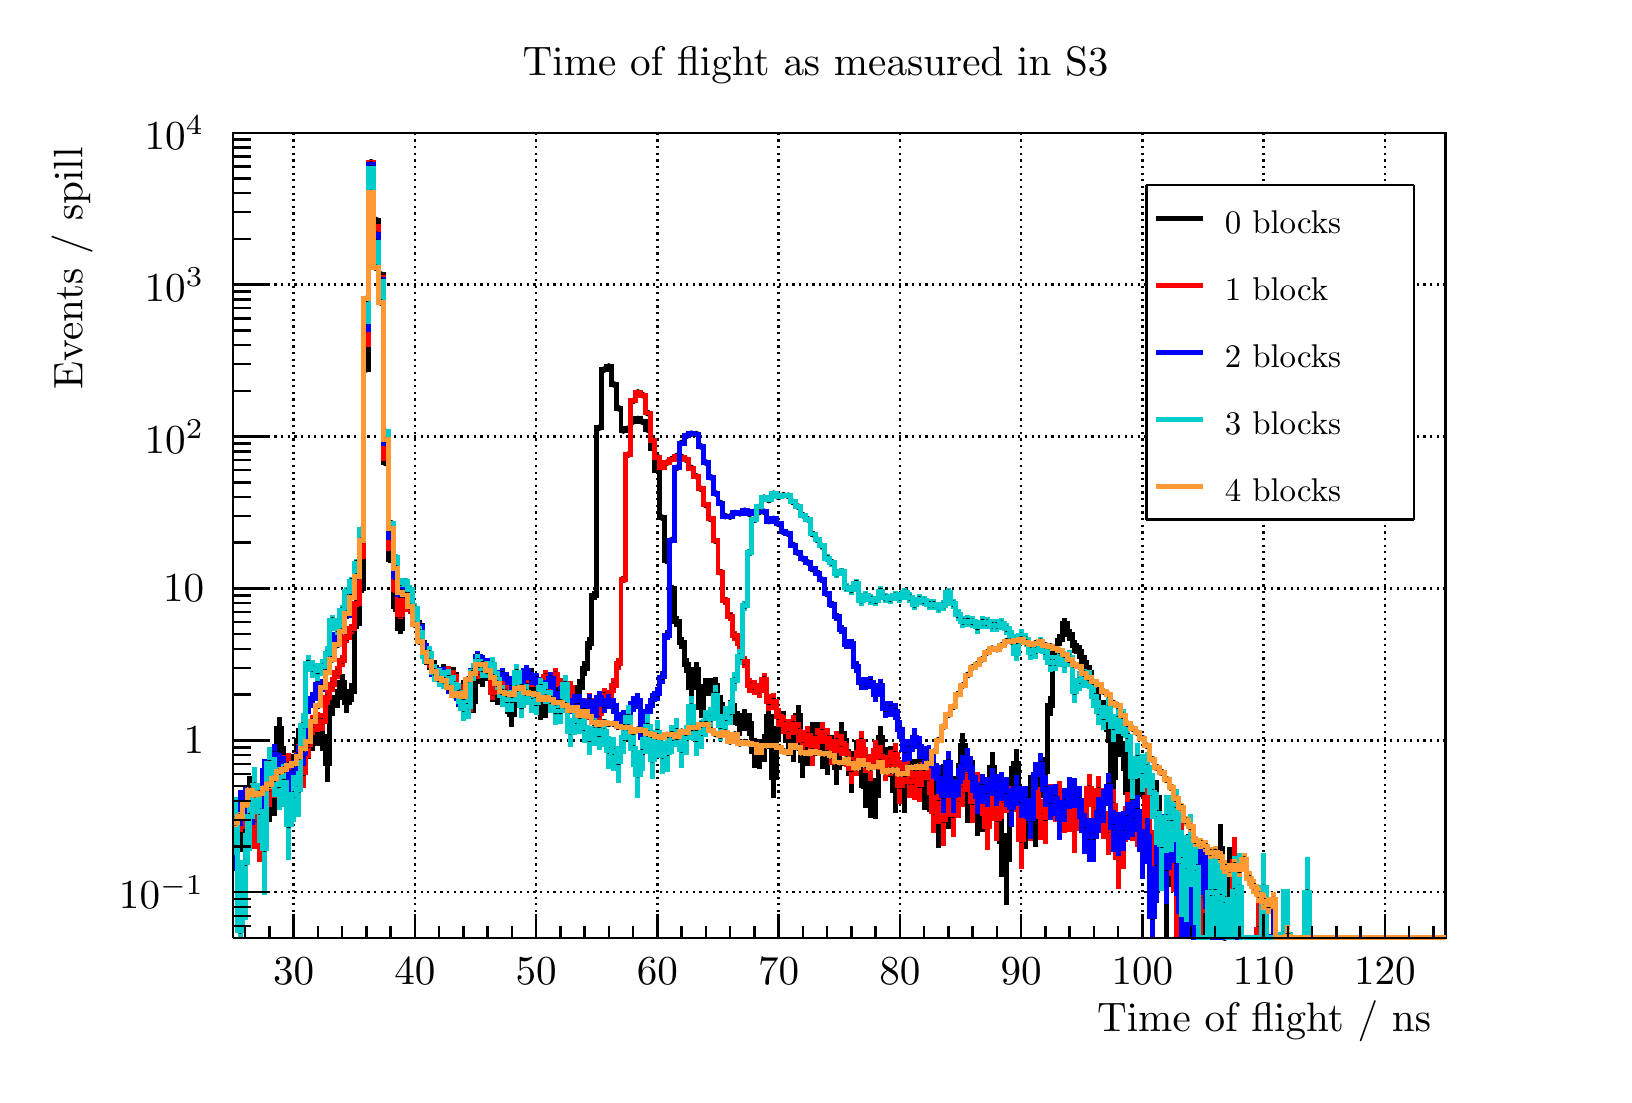
\begin{tikzpicture}
\pgfdeclareplotmark{cross} {
\pgfpathmoveto{\pgfpoint{-0.3\pgfplotmarksize}{\pgfplotmarksize}}
\pgfpathlineto{\pgfpoint{+0.3\pgfplotmarksize}{\pgfplotmarksize}}
\pgfpathlineto{\pgfpoint{+0.3\pgfplotmarksize}{0.3\pgfplotmarksize}}
\pgfpathlineto{\pgfpoint{+1\pgfplotmarksize}{0.3\pgfplotmarksize}}
\pgfpathlineto{\pgfpoint{+1\pgfplotmarksize}{-0.3\pgfplotmarksize}}
\pgfpathlineto{\pgfpoint{+0.3\pgfplotmarksize}{-0.3\pgfplotmarksize}}
\pgfpathlineto{\pgfpoint{+0.3\pgfplotmarksize}{-1.\pgfplotmarksize}}
\pgfpathlineto{\pgfpoint{-0.3\pgfplotmarksize}{-1.\pgfplotmarksize}}
\pgfpathlineto{\pgfpoint{-0.3\pgfplotmarksize}{-0.3\pgfplotmarksize}}
\pgfpathlineto{\pgfpoint{-1.\pgfplotmarksize}{-0.3\pgfplotmarksize}}
\pgfpathlineto{\pgfpoint{-1.\pgfplotmarksize}{0.3\pgfplotmarksize}}
\pgfpathlineto{\pgfpoint{-0.3\pgfplotmarksize}{0.3\pgfplotmarksize}}
\pgfpathclose
\pgfusepathqstroke
}
\pgfdeclareplotmark{cross*} {
\pgfpathmoveto{\pgfpoint{-0.3\pgfplotmarksize}{\pgfplotmarksize}}
\pgfpathlineto{\pgfpoint{+0.3\pgfplotmarksize}{\pgfplotmarksize}}
\pgfpathlineto{\pgfpoint{+0.3\pgfplotmarksize}{0.3\pgfplotmarksize}}
\pgfpathlineto{\pgfpoint{+1\pgfplotmarksize}{0.3\pgfplotmarksize}}
\pgfpathlineto{\pgfpoint{+1\pgfplotmarksize}{-0.3\pgfplotmarksize}}
\pgfpathlineto{\pgfpoint{+0.3\pgfplotmarksize}{-0.3\pgfplotmarksize}}
\pgfpathlineto{\pgfpoint{+0.3\pgfplotmarksize}{-1.\pgfplotmarksize}}
\pgfpathlineto{\pgfpoint{-0.3\pgfplotmarksize}{-1.\pgfplotmarksize}}
\pgfpathlineto{\pgfpoint{-0.3\pgfplotmarksize}{-0.3\pgfplotmarksize}}
\pgfpathlineto{\pgfpoint{-1.\pgfplotmarksize}{-0.3\pgfplotmarksize}}
\pgfpathlineto{\pgfpoint{-1.\pgfplotmarksize}{0.3\pgfplotmarksize}}
\pgfpathlineto{\pgfpoint{-0.3\pgfplotmarksize}{0.3\pgfplotmarksize}}
\pgfpathclose
\pgfusepathqfillstroke
}
\pgfdeclareplotmark{newstar} {
\pgfpathmoveto{\pgfqpoint{0pt}{\pgfplotmarksize}}
\pgfpathlineto{\pgfqpointpolar{44}{0.5\pgfplotmarksize}}
\pgfpathlineto{\pgfqpointpolar{18}{\pgfplotmarksize}}
\pgfpathlineto{\pgfqpointpolar{-20}{0.5\pgfplotmarksize}}
\pgfpathlineto{\pgfqpointpolar{-54}{\pgfplotmarksize}}
\pgfpathlineto{\pgfqpointpolar{-90}{0.5\pgfplotmarksize}}
\pgfpathlineto{\pgfqpointpolar{234}{\pgfplotmarksize}}
\pgfpathlineto{\pgfqpointpolar{198}{0.5\pgfplotmarksize}}
\pgfpathlineto{\pgfqpointpolar{162}{\pgfplotmarksize}}
\pgfpathlineto{\pgfqpointpolar{134}{0.5\pgfplotmarksize}}
\pgfpathclose
\pgfusepathqstroke
}
\pgfdeclareplotmark{newstar*} {
\pgfpathmoveto{\pgfqpoint{0pt}{\pgfplotmarksize}}
\pgfpathlineto{\pgfqpointpolar{44}{0.5\pgfplotmarksize}}
\pgfpathlineto{\pgfqpointpolar{18}{\pgfplotmarksize}}
\pgfpathlineto{\pgfqpointpolar{-20}{0.5\pgfplotmarksize}}
\pgfpathlineto{\pgfqpointpolar{-54}{\pgfplotmarksize}}
\pgfpathlineto{\pgfqpointpolar{-90}{0.5\pgfplotmarksize}}
\pgfpathlineto{\pgfqpointpolar{234}{\pgfplotmarksize}}
\pgfpathlineto{\pgfqpointpolar{198}{0.5\pgfplotmarksize}}
\pgfpathlineto{\pgfqpointpolar{162}{\pgfplotmarksize}}
\pgfpathlineto{\pgfqpointpolar{134}{0.5\pgfplotmarksize}}
\pgfpathclose
\pgfusepathqfillstroke
}
\definecolor{c}{rgb}{1,1,1};
\draw [color=c, fill=c] (0,0) rectangle (20,13.2798);
\draw [color=c, fill=c] (2.6,1.72637) rectangle (18,11.9518);
\definecolor{c}{rgb}{0,0,0};
\draw [c,line width=0.9] (2.6,1.72637) -- (2.6,11.9518) -- (18,11.9518) -- (18,1.72637) -- (2.6,1.72637);
\definecolor{c}{rgb}{1,1,1};
\draw [color=c, fill=c] (2.6,1.72637) rectangle (18,11.9518);
\definecolor{c}{rgb}{0,0,0};
\draw [c,line width=0.9] (2.6,1.72637) -- (2.6,11.9518) -- (18,11.9518) -- (18,1.72637) -- (2.6,1.72637);
\draw [c,line width=0.9] (2.6,1.72637) -- (18,1.72637);
\draw [c,dash pattern=on 0.80pt off 1.60pt ,line width=0.9] (3.37,11.9518) -- (3.37,1.72637);
\draw [c,dash pattern=on 0.80pt off 1.60pt ,line width=0.9] (4.91,11.9518) -- (4.91,1.72637);
\draw [c,dash pattern=on 0.80pt off 1.60pt ,line width=0.9] (6.45,11.9518) -- (6.45,1.72637);
\draw [c,dash pattern=on 0.80pt off 1.60pt ,line width=0.9] (7.99,11.9518) -- (7.99,1.72637);
\draw [c,dash pattern=on 0.80pt off 1.60pt ,line width=0.9] (9.53,11.9518) -- (9.53,1.72637);
\draw [c,dash pattern=on 0.80pt off 1.60pt ,line width=0.9] (11.07,11.9518) -- (11.07,1.72637);
\draw [c,dash pattern=on 0.80pt off 1.60pt ,line width=0.9] (12.61,11.9518) -- (12.61,1.72637);
\draw [c,dash pattern=on 0.80pt off 1.60pt ,line width=0.9] (14.15,11.9518) -- (14.15,1.72637);
\draw [c,dash pattern=on 0.80pt off 1.60pt ,line width=0.9] (15.69,11.9518) -- (15.69,1.72637);
\draw [c,dash pattern=on 0.80pt off 1.60pt ,line width=0.9] (17.23,11.9518) -- (17.23,1.72637);
\draw [c,dash pattern=on 0.80pt off 1.60pt ,line width=0.9] (3.37,11.9518) -- (3.37,1.72637);
\draw [c,dash pattern=on 0.80pt off 1.60pt ,line width=0.9] (17.23,11.9518) -- (17.23,1.72637);
\draw [c,line width=0.9] (2.6,1.72637) -- (2.6,11.9518);
\draw [c,dash pattern=on 0.80pt off 1.60pt ,line width=0.9] (18,2.30705) -- (2.6,2.30705);
\draw [c,dash pattern=on 0.80pt off 1.60pt ,line width=0.9] (18,4.236) -- (2.6,4.236);
\draw [c,dash pattern=on 0.80pt off 1.60pt ,line width=0.9] (18,6.16495) -- (2.6,6.16495);
\draw [c,dash pattern=on 0.80pt off 1.60pt ,line width=0.9] (18,8.0939) -- (2.6,8.0939);
\draw [c,dash pattern=on 0.80pt off 1.60pt ,line width=0.9] (18,10.0229) -- (2.6,10.0229);
\draw [c,dash pattern=on 0.80pt off 1.60pt ,line width=0.9] (18,11.9518) -- (2.6,11.9518);
\definecolor{c}{rgb}{0,0,0.6};
\draw [c,line width=0.9] (2.6,1.72637) -- (2.6616,1.72637) -- (2.6616,1.72637) -- (2.7232,1.72637) -- (2.7232,1.72637) -- (2.7848,1.72637) -- (2.7848,1.72637) -- (2.8464,1.72637) -- (2.8464,1.72637) -- (2.908,1.72637) -- (2.908,1.72637) --
 (2.9696,1.72637) -- (2.9696,1.72637) -- (3.0312,1.72637) -- (3.0312,1.72637) -- (3.0928,1.72637) -- (3.0928,1.72637) -- (3.1544,1.72637) -- (3.1544,1.72637) -- (3.216,1.72637) -- (3.216,1.72637) -- (3.2776,1.72637) -- (3.2776,1.72637) --
 (3.3392,1.72637) -- (3.3392,1.72637) -- (3.4008,1.72637) -- (3.4008,1.72637) -- (3.4624,1.72637) -- (3.4624,1.72637) -- (3.524,1.72637) -- (3.524,1.72637) -- (3.5856,1.72637) -- (3.5856,1.72637) -- (3.6472,1.72637) -- (3.6472,1.72637) --
 (3.7088,1.72637) -- (3.7088,1.72637) -- (3.7704,1.72637) -- (3.7704,1.72637) -- (3.832,1.72637) -- (3.832,1.72637) -- (3.8936,1.72637) -- (3.8936,1.72637) -- (3.9552,1.72637) -- (3.9552,1.72637) -- (4.0168,1.72637) -- (4.0168,1.72637) --
 (4.0784,1.72637) -- (4.0784,1.72637) -- (4.14,1.72637) -- (4.14,1.72637) -- (4.2016,1.72637) -- (4.2016,1.72637) -- (4.2632,1.72637) -- (4.2632,1.72637) -- (4.3248,1.72637) -- (4.3248,1.72637) -- (4.3864,1.72637) -- (4.3864,1.72637) --
 (4.448,1.72637) -- (4.448,1.72637) -- (4.5096,1.72637) -- (4.5096,1.72637) -- (4.5712,1.72637) -- (4.5712,1.72637) -- (4.6328,1.72637) -- (4.6328,1.72637) -- (4.6944,1.72637) -- (4.6944,1.72637) -- (4.756,1.72637) -- (4.756,1.72637) --
 (4.8176,1.72637) -- (4.8176,1.72637) -- (4.8792,1.72637) -- (4.8792,1.72637) -- (4.9408,1.72637) -- (4.9408,1.72637) -- (5.0024,1.72637) -- (5.0024,1.72637) -- (5.064,1.72637) -- (5.064,1.72637) -- (5.1256,1.72637) -- (5.1256,1.72637) --
 (5.1872,1.72637) -- (5.1872,1.72637) -- (5.2488,1.72637) -- (5.2488,1.72637) -- (5.3104,1.72637) -- (5.3104,1.72637) -- (5.372,1.72637) -- (5.372,1.72637) -- (5.4336,1.72637) -- (5.4336,1.72637) -- (5.4952,1.72637) -- (5.4952,1.72637) --
 (5.5568,1.72637) -- (5.5568,1.72637) -- (5.6184,1.72637) -- (5.6184,1.72637) -- (5.68,1.72637) -- (5.68,1.72637) -- (5.7416,1.72637) -- (5.7416,1.72637) -- (5.8032,1.72637) -- (5.8032,1.72637) -- (5.8648,1.72637) -- (5.8648,1.72637) --
 (5.9264,1.72637) -- (5.9264,1.72637) -- (5.988,1.72637) -- (5.988,1.72637) -- (6.0496,1.72637) -- (6.0496,1.72637) -- (6.1112,1.72637) -- (6.1112,1.72637) -- (6.1728,1.72637) -- (6.1728,1.72637) -- (6.2344,1.72637) -- (6.2344,1.72637) --
 (6.296,1.72637) -- (6.296,1.72637) -- (6.3576,1.72637) -- (6.3576,1.72637) -- (6.4192,1.72637) -- (6.4192,1.72637) -- (6.4808,1.72637) -- (6.4808,1.72637) -- (6.5424,1.72637) -- (6.5424,1.72637) -- (6.604,1.72637) -- (6.604,1.72637) --
 (6.6656,1.72637) -- (6.6656,1.72637) -- (6.7272,1.72637) -- (6.7272,1.72637) -- (6.7888,1.72637) -- (6.7888,1.72637) -- (6.8504,1.72637) -- (6.8504,1.72637) -- (6.912,1.72637) -- (6.912,1.72637) -- (6.9736,1.72637) -- (6.9736,1.72637) --
 (7.0352,1.72637) -- (7.0352,1.72637) -- (7.0968,1.72637) -- (7.0968,1.72637) -- (7.1584,1.72637) -- (7.1584,1.72637) -- (7.22,1.72637) -- (7.22,1.72637) -- (7.2816,1.72637) -- (7.2816,1.72637) -- (7.3432,1.72637) -- (7.3432,1.72637) --
 (7.4048,1.72637) -- (7.4048,1.72637) -- (7.4664,1.72637) -- (7.4664,1.72637) -- (7.528,1.72637) -- (7.528,1.72637) -- (7.5896,1.72637) -- (7.5896,1.72637) -- (7.6512,1.72637) -- (7.6512,1.72637) -- (7.7128,1.72637) -- (7.7128,1.72637) --
 (7.7744,1.72637) -- (7.7744,1.72637) -- (7.836,1.72637) -- (7.836,1.72637) -- (7.8976,1.72637) -- (7.8976,1.72637) -- (7.9592,1.72637) -- (7.9592,1.72637) -- (8.0208,1.72637) -- (8.0208,1.72637) -- (8.0824,1.72637) -- (8.0824,1.72637) --
 (8.144,1.72637) -- (8.144,1.72637) -- (8.2056,1.72637) -- (8.2056,1.72637) -- (8.2672,1.72637) -- (8.2672,1.72637) -- (8.3288,1.72637) -- (8.3288,1.72637) -- (8.3904,1.72637) -- (8.3904,1.72637) -- (8.452,1.72637) -- (8.452,1.72637) --
 (8.5136,1.72637) -- (8.5136,1.72637) -- (8.5752,1.72637) -- (8.5752,1.72637) -- (8.6368,1.72637) -- (8.6368,1.72637) -- (8.6984,1.72637) -- (8.6984,1.72637) -- (8.76,1.72637) -- (8.76,1.72637) -- (8.8216,1.72637) -- (8.8216,1.72637) --
 (8.8832,1.72637) -- (8.8832,1.72637) -- (8.9448,1.72637) -- (8.9448,1.72637) -- (9.0064,1.72637) -- (9.0064,1.72637) -- (9.068,1.72637) -- (9.068,1.72637) -- (9.1296,1.72637) -- (9.1296,1.72637) -- (9.1912,1.72637) -- (9.1912,1.72637) --
 (9.2528,1.72637) -- (9.2528,1.72637) -- (9.3144,1.72637) -- (9.3144,1.72637) -- (9.376,1.72637) -- (9.376,1.72637) -- (9.4376,1.72637) -- (9.4376,1.72637) -- (9.4992,1.72637) -- (9.4992,1.72637) -- (9.5608,1.72637) -- (9.5608,1.72637) --
 (9.6224,1.72637) -- (9.6224,1.72637) -- (9.684,1.72637) -- (9.684,1.72637) -- (9.7456,1.72637) -- (9.7456,1.72637) -- (9.8072,1.72637) -- (9.8072,1.72637) -- (9.8688,1.72637) -- (9.8688,1.72637) -- (9.9304,1.72637) -- (9.9304,1.72637) --
 (9.992,1.72637) -- (9.992,1.72637) -- (10.0536,1.72637) -- (10.0536,1.72637) -- (10.1152,1.72637) -- (10.1152,1.72637) -- (10.1768,1.72637) -- (10.1768,1.72637) -- (10.2384,1.72637) -- (10.2384,1.72637) -- (10.3,1.72637) -- (10.3,1.72637) --
 (10.3616,1.72637) -- (10.3616,1.72637) -- (10.4232,1.72637) -- (10.4232,1.72637) -- (10.4848,1.72637) -- (10.4848,1.72637) -- (10.5464,1.72637) -- (10.5464,1.72637) -- (10.608,1.72637) -- (10.608,1.72637) -- (10.6696,1.72637) -- (10.6696,1.72637) --
 (10.7312,1.72637) -- (10.7312,1.72637) -- (10.7928,1.72637) -- (10.7928,1.72637) -- (10.8544,1.72637) -- (10.8544,1.72637) -- (10.916,1.72637) -- (10.916,1.72637) -- (10.9776,1.72637) -- (10.9776,1.72637) -- (11.0392,1.72637) -- (11.0392,1.72637) --
 (11.1008,1.72637) -- (11.1008,1.72637) -- (11.1624,1.72637) -- (11.1624,1.72637) -- (11.224,1.72637) -- (11.224,1.72637) -- (11.2856,1.72637) -- (11.2856,1.72637) -- (11.3472,1.72637) -- (11.3472,1.72637) -- (11.4088,1.72637) -- (11.4088,1.72637) --
 (11.4704,1.72637) -- (11.4704,1.72637) -- (11.532,1.72637) -- (11.532,1.72637) -- (11.5936,1.72637) -- (11.5936,1.72637) -- (11.6552,1.72637) -- (11.6552,1.72637) -- (11.7168,1.72637) -- (11.7168,1.72637) -- (11.7784,1.72637) -- (11.7784,1.72637) --
 (11.84,1.72637) -- (11.84,1.72637) -- (11.9016,1.72637) -- (11.9016,1.72637) -- (11.9632,1.72637) -- (11.9632,1.72637) -- (12.0248,1.72637) -- (12.0248,1.72637) -- (12.0864,1.72637) -- (12.0864,1.72637) -- (12.148,1.72637) -- (12.148,1.72637) --
 (12.2096,1.72637) -- (12.2096,1.72637) -- (12.2712,1.72637) -- (12.2712,1.72637) -- (12.3328,1.72637) -- (12.3328,1.72637) -- (12.3944,1.72637) -- (12.3944,1.72637) -- (12.456,1.72637) -- (12.456,1.72637) -- (12.5176,1.72637) -- (12.5176,1.72637) --
 (12.5792,1.72637) -- (12.5792,1.72637) -- (12.6408,1.72637) -- (12.6408,1.72637) -- (12.7024,1.72637) -- (12.7024,1.72637) -- (12.764,1.72637) -- (12.764,1.72637) -- (12.8256,1.72637) -- (12.8256,1.72637) -- (12.8872,1.72637) -- (12.8872,1.72637) --
 (12.9488,1.72637) -- (12.9488,1.72637) -- (13.0104,1.72637) -- (13.0104,1.72637) -- (13.072,1.72637) -- (13.072,1.72637) -- (13.1336,1.72637) -- (13.1336,1.72637) -- (13.1952,1.72637) -- (13.1952,1.72637) -- (13.2568,1.72637) -- (13.2568,1.72637) --
 (13.3184,1.72637) -- (13.3184,1.72637) -- (13.38,1.72637) -- (13.38,1.72637) -- (13.4416,1.72637) -- (13.4416,1.72637) -- (13.5032,1.72637) -- (13.5032,1.72637) -- (13.5648,1.72637) -- (13.5648,1.72637) -- (13.6264,1.72637) -- (13.6264,1.72637) --
 (13.688,1.72637) -- (13.688,1.72637) -- (13.7496,1.72637) -- (13.7496,1.72637) -- (13.8112,1.72637) -- (13.8112,1.72637) -- (13.8728,1.72637) -- (13.8728,1.72637) -- (13.9344,1.72637) -- (13.9344,1.72637) -- (13.996,1.72637) -- (13.996,1.72637) --
 (14.0576,1.72637) -- (14.0576,1.72637) -- (14.1192,1.72637) -- (14.1192,1.72637) -- (14.1808,1.72637) -- (14.1808,1.72637) -- (14.2424,1.72637) -- (14.2424,1.72637) -- (14.304,1.72637) -- (14.304,1.72637) -- (14.3656,1.72637) -- (14.3656,1.72637) --
 (14.4272,1.72637) -- (14.4272,1.72637) -- (14.4888,1.72637) -- (14.4888,1.72637) -- (14.5504,1.72637) -- (14.5504,1.72637) -- (14.612,1.72637) -- (14.612,1.72637) -- (14.6736,1.72637) -- (14.6736,1.72637) -- (14.7352,1.72637) -- (14.7352,1.72637) --
 (14.7968,1.72637) -- (14.7968,1.72637) -- (14.8584,1.72637) -- (14.8584,1.72637) -- (14.92,1.72637) -- (14.92,1.72637) -- (14.9816,1.72637) -- (14.9816,1.72637) -- (15.0432,1.72637) -- (15.0432,1.72637) -- (15.1048,1.72637) -- (15.1048,1.72637) --
 (15.1664,1.72637) -- (15.1664,1.72637) -- (15.228,1.72637) -- (15.228,1.72637) -- (15.2896,1.72637) -- (15.2896,1.72637) -- (15.3512,1.72637) -- (15.3512,1.72637) -- (15.4128,1.72637) -- (15.4128,1.72637) -- (15.4744,1.72637) -- (15.4744,1.72637) --
 (15.536,1.72637) -- (15.536,1.72637) -- (15.5976,1.72637) -- (15.5976,1.72637) -- (15.6592,1.72637) -- (15.6592,1.72637) -- (15.7208,1.72637) -- (15.7208,1.72637) -- (15.7824,1.72637) -- (15.7824,1.72637) -- (15.844,1.72637) -- (15.844,1.72637) --
 (15.9056,1.72637) -- (15.9056,1.72637) -- (15.9672,1.72637) -- (15.9672,1.72637) -- (16.0288,1.72637) -- (16.0288,1.72637) -- (16.0904,1.72637) -- (16.0904,1.72637) -- (16.152,1.72637) -- (16.152,1.72637) -- (16.2136,1.72637) -- (16.2136,1.72637) --
 (16.2752,1.72637) -- (16.2752,1.72637) -- (16.3368,1.72637) -- (16.3368,1.72637) -- (16.3984,1.72637) -- (16.3984,1.72637) -- (16.46,1.72637) -- (16.46,1.72637) -- (16.5216,1.72637) -- (16.5216,1.72637) -- (16.5832,1.72637) -- (16.5832,1.72637) --
 (16.6448,1.72637) -- (16.6448,1.72637) -- (16.7064,1.72637) -- (16.7064,1.72637) -- (16.768,1.72637) -- (16.768,1.72637) -- (16.8296,1.72637) -- (16.8296,1.72637) -- (16.8912,1.72637) -- (16.8912,1.72637) -- (16.9528,1.72637) -- (16.9528,1.72637) --
 (17.0144,1.72637) -- (17.0144,1.72637) -- (17.076,1.72637) -- (17.076,1.72637) -- (17.1376,1.72637) -- (17.1376,1.72637) -- (17.1992,1.72637) -- (17.1992,1.72637) -- (17.2608,1.72637) -- (17.2608,1.72637) -- (17.3224,1.72637) -- (17.3224,1.72637) --
 (17.384,1.72637) -- (17.384,1.72637) -- (17.4456,1.72637) -- (17.4456,1.72637) -- (17.5072,1.72637) -- (17.5072,1.72637) -- (17.5688,1.72637) -- (17.5688,1.72637) -- (17.6304,1.72637) -- (17.6304,1.72637) -- (17.692,1.72637) -- (17.692,1.72637) --
 (17.7536,1.72637) -- (17.7536,1.72637) -- (17.8152,1.72637) -- (17.8152,1.72637) -- (17.8768,1.72637) -- (17.8768,1.72637) -- (17.9384,1.72637) -- (17.9384,1.72637) -- (18,1.72637);
\definecolor{c}{rgb}{0,0,0};
\draw [c,line width=0.9] (2.6,1.72637) -- (18,1.72637);
\draw [c,line width=0.9] (3.37,2.03314) -- (3.37,1.72637);
\draw [c,line width=0.9] (3.678,1.87975) -- (3.678,1.72637);
\draw [c,line width=0.9] (3.986,1.87975) -- (3.986,1.72637);
\draw [c,line width=0.9] (4.294,1.87975) -- (4.294,1.72637);
\draw [c,line width=0.9] (4.602,1.87975) -- (4.602,1.72637);
\draw [c,line width=0.9] (4.91,2.03314) -- (4.91,1.72637);
\draw [c,line width=0.9] (5.218,1.87975) -- (5.218,1.72637);
\draw [c,line width=0.9] (5.526,1.87975) -- (5.526,1.72637);
\draw [c,line width=0.9] (5.834,1.87975) -- (5.834,1.72637);
\draw [c,line width=0.9] (6.142,1.87975) -- (6.142,1.72637);
\draw [c,line width=0.9] (6.45,2.03314) -- (6.45,1.72637);
\draw [c,line width=0.9] (6.758,1.87975) -- (6.758,1.72637);
\draw [c,line width=0.9] (7.066,1.87975) -- (7.066,1.72637);
\draw [c,line width=0.9] (7.374,1.87975) -- (7.374,1.72637);
\draw [c,line width=0.9] (7.682,1.87975) -- (7.682,1.72637);
\draw [c,line width=0.9] (7.99,2.03314) -- (7.99,1.72637);
\draw [c,line width=0.9] (8.298,1.87975) -- (8.298,1.72637);
\draw [c,line width=0.9] (8.606,1.87975) -- (8.606,1.72637);
\draw [c,line width=0.9] (8.914,1.87975) -- (8.914,1.72637);
\draw [c,line width=0.9] (9.222,1.87975) -- (9.222,1.72637);
\draw [c,line width=0.9] (9.53,2.03314) -- (9.53,1.72637);
\draw [c,line width=0.9] (9.838,1.87975) -- (9.838,1.72637);
\draw [c,line width=0.9] (10.146,1.87975) -- (10.146,1.72637);
\draw [c,line width=0.9] (10.454,1.87975) -- (10.454,1.72637);
\draw [c,line width=0.9] (10.762,1.87975) -- (10.762,1.72637);
\draw [c,line width=0.9] (11.07,2.03314) -- (11.07,1.72637);
\draw [c,line width=0.9] (11.378,1.87975) -- (11.378,1.72637);
\draw [c,line width=0.9] (11.686,1.87975) -- (11.686,1.72637);
\draw [c,line width=0.9] (11.994,1.87975) -- (11.994,1.72637);
\draw [c,line width=0.9] (12.302,1.87975) -- (12.302,1.72637);
\draw [c,line width=0.9] (12.61,2.03314) -- (12.61,1.72637);
\draw [c,line width=0.9] (12.918,1.87975) -- (12.918,1.72637);
\draw [c,line width=0.9] (13.226,1.87975) -- (13.226,1.72637);
\draw [c,line width=0.9] (13.534,1.87975) -- (13.534,1.72637);
\draw [c,line width=0.9] (13.842,1.87975) -- (13.842,1.72637);
\draw [c,line width=0.9] (14.15,2.03314) -- (14.15,1.72637);
\draw [c,line width=0.9] (14.458,1.87975) -- (14.458,1.72637);
\draw [c,line width=0.9] (14.766,1.87975) -- (14.766,1.72637);
\draw [c,line width=0.9] (15.074,1.87975) -- (15.074,1.72637);
\draw [c,line width=0.9] (15.382,1.87975) -- (15.382,1.72637);
\draw [c,line width=0.9] (15.69,2.03314) -- (15.69,1.72637);
\draw [c,line width=0.9] (15.998,1.87975) -- (15.998,1.72637);
\draw [c,line width=0.9] (16.306,1.87975) -- (16.306,1.72637);
\draw [c,line width=0.9] (16.614,1.87975) -- (16.614,1.72637);
\draw [c,line width=0.9] (16.922,1.87975) -- (16.922,1.72637);
\draw [c,line width=0.9] (17.23,2.03314) -- (17.23,1.72637);
\draw [c,line width=0.9] (3.37,2.03314) -- (3.37,1.72637);
\draw [c,line width=0.9] (3.062,1.87975) -- (3.062,1.72637);
\draw [c,line width=0.9] (2.754,1.87975) -- (2.754,1.72637);
\draw [c,line width=0.9] (17.23,2.03314) -- (17.23,1.72637);
\draw [c,line width=0.9] (17.538,1.87975) -- (17.538,1.72637);
\draw [c,line width=0.9] (17.846,1.87975) -- (17.846,1.72637);
\draw [anchor=base] (3.37,1.12878) node[scale=1.48659, color=c, rotate=0]{30};
\draw [anchor=base] (4.91,1.12878) node[scale=1.48659, color=c, rotate=0]{40};
\draw [anchor=base] (6.45,1.12878) node[scale=1.48659, color=c, rotate=0]{50};
\draw [anchor=base] (7.99,1.12878) node[scale=1.48659, color=c, rotate=0]{60};
\draw [anchor=base] (9.53,1.12878) node[scale=1.48659, color=c, rotate=0]{70};
\draw [anchor=base] (11.07,1.12878) node[scale=1.48659, color=c, rotate=0]{80};
\draw [anchor=base] (12.61,1.12878) node[scale=1.48659, color=c, rotate=0]{90};
\draw [anchor=base] (14.15,1.12878) node[scale=1.48659, color=c, rotate=0]{100};
\draw [anchor=base] (15.69,1.12878) node[scale=1.48659, color=c, rotate=0]{110};
\draw [anchor=base] (17.23,1.12878) node[scale=1.48659, color=c, rotate=0]{120};
\draw [anchor= east] (18,0.663989) node[scale=1.48659, color=c, rotate=0]{ Time of flight / ns};
\draw [c,line width=0.9] (2.6,1.72637) -- (2.6,11.9518);
\draw [c,line width=0.9] (2.831,1.72637) -- (2.6,1.72637);
\draw [c,line width=0.9] (2.831,1.87911) -- (2.6,1.87911);
\draw [c,line width=0.9] (2.831,2.00825) -- (2.6,2.00825);
\draw [c,line width=0.9] (2.831,2.12011) -- (2.6,2.12011);
\draw [c,line width=0.9] (2.831,2.21878) -- (2.6,2.21878);
\draw [c,line width=0.9] (3.062,2.30705) -- (2.6,2.30705);
\draw [anchor= east] (2.42,2.30705) node[scale=1.48659, color=c, rotate=0]{$10^{-1}$};
\draw [c,line width=0.9] (2.831,2.88772) -- (2.6,2.88772);
\draw [c,line width=0.9] (2.831,3.22739) -- (2.6,3.22739);
\draw [c,line width=0.9] (2.831,3.46839) -- (2.6,3.46839);
\draw [c,line width=0.9] (2.831,3.65533) -- (2.6,3.65533);
\draw [c,line width=0.9] (2.831,3.80806) -- (2.6,3.80806);
\draw [c,line width=0.9] (2.831,3.9372) -- (2.6,3.9372);
\draw [c,line width=0.9] (2.831,4.04906) -- (2.6,4.04906);
\draw [c,line width=0.9] (2.831,4.14773) -- (2.6,4.14773);
\draw [c,line width=0.9] (3.062,4.236) -- (2.6,4.236);
\draw [anchor= east] (2.42,4.236) node[scale=1.48659, color=c, rotate=0]{1};
\draw [c,line width=0.9] (2.831,4.81667) -- (2.6,4.81667);
\draw [c,line width=0.9] (2.831,5.15634) -- (2.6,5.15634);
\draw [c,line width=0.9] (2.831,5.39734) -- (2.6,5.39734);
\draw [c,line width=0.9] (2.831,5.58428) -- (2.6,5.58428);
\draw [c,line width=0.9] (2.831,5.73702) -- (2.6,5.73702);
\draw [c,line width=0.9] (2.831,5.86615) -- (2.6,5.86615);
\draw [c,line width=0.9] (2.831,5.97802) -- (2.6,5.97802);
\draw [c,line width=0.9] (2.831,6.07669) -- (2.6,6.07669);
\draw [c,line width=0.9] (3.062,6.16495) -- (2.6,6.16495);
\draw [anchor= east] (2.42,6.16495) node[scale=1.48659, color=c, rotate=0]{10};
\draw [c,line width=0.9] (2.831,6.74562) -- (2.6,6.74562);
\draw [c,line width=0.9] (2.831,7.0853) -- (2.6,7.0853);
\draw [c,line width=0.9] (2.831,7.3263) -- (2.6,7.3263);
\draw [c,line width=0.9] (2.831,7.51323) -- (2.6,7.51323);
\draw [c,line width=0.9] (2.831,7.66597) -- (2.6,7.66597);
\draw [c,line width=0.9] (2.831,7.7951) -- (2.6,7.7951);
\draw [c,line width=0.9] (2.831,7.90697) -- (2.6,7.90697);
\draw [c,line width=0.9] (2.831,8.00564) -- (2.6,8.00564);
\draw [c,line width=0.9] (3.062,8.0939) -- (2.6,8.0939);
\draw [anchor= east] (2.42,8.0939) node[scale=1.48659, color=c, rotate=0]{$10^{2}$};
\draw [c,line width=0.9] (2.831,8.67458) -- (2.6,8.67458);
\draw [c,line width=0.9] (2.831,9.01425) -- (2.6,9.01425);
\draw [c,line width=0.9] (2.831,9.25525) -- (2.6,9.25525);
\draw [c,line width=0.9] (2.831,9.44218) -- (2.6,9.44218);
\draw [c,line width=0.9] (2.831,9.59492) -- (2.6,9.59492);
\draw [c,line width=0.9] (2.831,9.72406) -- (2.6,9.72406);
\draw [c,line width=0.9] (2.831,9.83592) -- (2.6,9.83592);
\draw [c,line width=0.9] (2.831,9.93459) -- (2.6,9.93459);
\draw [c,line width=0.9] (3.062,10.0229) -- (2.6,10.0229);
\draw [anchor= east] (2.42,10.0229) node[scale=1.48659, color=c, rotate=0]{$10^{3}$};
\draw [c,line width=0.9] (2.831,10.6035) -- (2.6,10.6035);
\draw [c,line width=0.9] (2.831,10.9432) -- (2.6,10.9432);
\draw [c,line width=0.9] (2.831,11.1842) -- (2.6,11.1842);
\draw [c,line width=0.9] (2.831,11.3711) -- (2.6,11.3711);
\draw [c,line width=0.9] (2.831,11.5239) -- (2.6,11.5239);
\draw [c,line width=0.9] (2.831,11.653) -- (2.6,11.653);
\draw [c,line width=0.9] (2.831,11.7649) -- (2.6,11.7649);
\draw [c,line width=0.9] (2.831,11.8635) -- (2.6,11.8635);
\draw [c,line width=0.9] (3.062,11.9518) -- (2.6,11.9518);
\draw [anchor= east] (2.42,11.9518) node[scale=1.48659, color=c, rotate=0]{$10^{4}$};
\draw [anchor= east] (0.555823,11.9518) node[scale=1.48659, color=c, rotate=90]{ Events / spill};
\draw [c,line width=1.8] (2.6308,2.77114) -- (2.6308,3.17174);
\draw [c,line width=1.8] (2.6308,3.17174) -- (2.6308,3.44162);
\foreach \P in {(2.6308,3.17174)}{\draw[mark options={color=c,fill=c},mark size=2.402402pt,mark=*,mark size=1pt] plot coordinates {\P};}
\draw [c,line width=1.8] (2.6924,3.0256) -- (2.6924,3.36758);
\draw [c,line width=1.8] (2.6924,3.36758) -- (2.6924,3.60974);
\foreach \P in {(2.6924,3.36758)}{\draw[mark options={color=c,fill=c},mark size=2.402402pt,mark=*,mark size=1pt] plot coordinates {\P};}
\draw [c,line width=1.8] (2.754,2.34776) -- (2.754,2.8466);
\draw [c,line width=1.8] (2.754,2.8466) -- (2.754,3.15711);
\foreach \P in {(2.754,2.8466)}{\draw[mark options={color=c,fill=c},mark size=2.402402pt,mark=*,mark size=1pt] plot coordinates {\P};}
\draw [c,line width=1.8] (2.8156,3.25286) -- (2.8156,3.5561);
\draw [c,line width=1.8] (2.8156,3.5561) -- (2.8156,3.77828);
\foreach \P in {(2.8156,3.5561)}{\draw[mark options={color=c,fill=c},mark size=2.402402pt,mark=*,mark size=1pt] plot coordinates {\P};}
\draw [c,line width=1.8] (2.8772,3.22715) -- (2.8772,3.53036);
\draw [c,line width=1.8] (2.8772,3.53036) -- (2.8772,3.75252);
\foreach \P in {(2.8772,3.53036)}{\draw[mark options={color=c,fill=c},mark size=2.402402pt,mark=*,mark size=1pt] plot coordinates {\P};}
\draw [c,line width=1.8] (2.9388,2.91016) -- (2.9388,3.27672);
\draw [c,line width=1.8] (2.9388,3.27672) -- (2.9388,3.53085);
\foreach \P in {(2.9388,3.27672)}{\draw[mark options={color=c,fill=c},mark size=2.402402pt,mark=*,mark size=1pt] plot coordinates {\P};}
\draw [c,line width=1.8] (3.0004,3.43134) -- (3.0004,3.70458);
\draw [c,line width=1.8] (3.0004,3.70458) -- (3.0004,3.91027);
\foreach \P in {(3.0004,3.70458)}{\draw[mark options={color=c,fill=c},mark size=2.402402pt,mark=*,mark size=1pt] plot coordinates {\P};}
\draw [c,line width=1.8] (3.062,3.2046) -- (3.062,3.52779);
\draw [c,line width=1.8] (3.062,3.52779) -- (3.062,3.76042);
\foreach \P in {(3.062,3.52779)}{\draw[mark options={color=c,fill=c},mark size=2.402402pt,mark=*,mark size=1pt] plot coordinates {\P};}
\draw [c,line width=1.8] (3.1236,3.27619) -- (3.1236,3.58064);
\draw [c,line width=1.8] (3.1236,3.58064) -- (3.1236,3.80345);
\foreach \P in {(3.1236,3.58064)}{\draw[mark options={color=c,fill=c},mark size=2.402402pt,mark=*,mark size=1pt] plot coordinates {\P};}
\draw [c,line width=1.8] (3.1852,4.21537) -- (3.1852,4.38546);
\draw [c,line width=1.8] (3.1852,4.38546) -- (3.1852,4.52677);
\foreach \P in {(3.1852,4.38546)}{\draw[mark options={color=c,fill=c},mark size=2.402402pt,mark=*,mark size=1pt] plot coordinates {\P};}
\draw [c,line width=1.8] (3.2468,3.75588) -- (3.2468,3.9829);
\draw [c,line width=1.8] (3.2468,3.9829) -- (3.2468,4.16133);
\foreach \P in {(3.2468,3.9829)}{\draw[mark options={color=c,fill=c},mark size=2.402402pt,mark=*,mark size=1pt] plot coordinates {\P};}
\draw [c,line width=1.8] (3.3084,3.23882) -- (3.3084,3.54102);
\draw [c,line width=1.8] (3.3084,3.54102) -- (3.3084,3.76265);
\foreach \P in {(3.3084,3.54102)}{\draw[mark options={color=c,fill=c},mark size=2.402402pt,mark=*,mark size=1pt] plot coordinates {\P};}
\draw [c,line width=1.8] (3.37,3.63627) -- (3.37,3.87885);
\draw [c,line width=1.8] (3.37,3.87885) -- (3.37,4.06673);
\foreach \P in {(3.37,3.87885)}{\draw[mark options={color=c,fill=c},mark size=2.402402pt,mark=*,mark size=1pt] plot coordinates {\P};}
\draw [c,line width=1.8] (3.4316,4.04533) -- (3.4316,4.23339);
\draw [c,line width=1.8] (3.4316,4.23339) -- (3.4316,4.38688);
\foreach \P in {(3.4316,4.23339)}{\draw[mark options={color=c,fill=c},mark size=2.402402pt,mark=*,mark size=1pt] plot coordinates {\P};}
\draw [c,line width=1.8] (3.4932,3.95685) -- (3.4932,4.15415);
\draw [c,line width=1.8] (3.4932,4.15415) -- (3.4932,4.31373);
\foreach \P in {(3.4932,4.15415)}{\draw[mark options={color=c,fill=c},mark size=2.402402pt,mark=*,mark size=1pt] plot coordinates {\P};}
\draw [c,line width=1.8] (3.5548,3.99515) -- (3.5548,4.18816);
\draw [c,line width=1.8] (3.5548,4.18816) -- (3.5548,4.34492);
\foreach \P in {(3.5548,4.18816)}{\draw[mark options={color=c,fill=c},mark size=2.402402pt,mark=*,mark size=1pt] plot coordinates {\P};}
\draw [c,line width=1.8] (3.6164,4.1066) -- (3.6164,4.28665);
\draw [c,line width=1.8] (3.6164,4.28665) -- (3.6164,4.43476);
\foreach \P in {(3.6164,4.28665)}{\draw[mark options={color=c,fill=c},mark size=2.402402pt,mark=*,mark size=1pt] plot coordinates {\P};}
\draw [c,line width=1.8] (3.678,4.1654) -- (3.678,4.33867);
\draw [c,line width=1.8] (3.678,4.33867) -- (3.678,4.48218);
\foreach \P in {(3.678,4.33867)}{\draw[mark options={color=c,fill=c},mark size=2.402402pt,mark=*,mark size=1pt] plot coordinates {\P};}
\draw [c,line width=1.8] (3.7396,4.09828) -- (3.7396,4.27861);
\draw [c,line width=1.8] (3.7396,4.27861) -- (3.7396,4.42692);
\foreach \P in {(3.7396,4.27861)}{\draw[mark options={color=c,fill=c},mark size=2.402402pt,mark=*,mark size=1pt] plot coordinates {\P};}
\draw [c,line width=1.8] (3.8012,3.71294) -- (3.8012,3.93969);
\draw [c,line width=1.8] (3.8012,3.93969) -- (3.8012,4.11796);
\foreach \P in {(3.8012,3.93969)}{\draw[mark options={color=c,fill=c},mark size=2.402402pt,mark=*,mark size=1pt] plot coordinates {\P};}
\draw [c,line width=1.8] (3.8628,4.54888) -- (3.8628,4.68877);
\draw [c,line width=1.8] (3.8628,4.68877) -- (3.8628,4.80861);
\foreach \P in {(3.8628,4.68877)}{\draw[mark options={color=c,fill=c},mark size=2.402402pt,mark=*,mark size=1pt] plot coordinates {\P};}
\draw [c,line width=1.8] (3.9244,4.64709) -- (3.9244,4.77849);
\draw [c,line width=1.8] (3.9244,4.77849) -- (3.9244,4.89204);
\foreach \P in {(3.9244,4.77849)}{\draw[mark options={color=c,fill=c},mark size=2.402402pt,mark=*,mark size=1pt] plot coordinates {\P};}
\draw [c,line width=1.8] (3.986,4.859) -- (3.986,4.97676);
\draw [c,line width=1.8] (3.986,4.97676) -- (3.986,5.07999);
\foreach \P in {(3.986,4.97676)}{\draw[mark options={color=c,fill=c},mark size=2.402402pt,mark=*,mark size=1pt] plot coordinates {\P};}
\draw [c,line width=1.8] (4.0476,4.58011) -- (4.0476,4.71618);
\draw [c,line width=1.8] (4.0476,4.71618) -- (4.0476,4.83322);
\foreach \P in {(4.0476,4.71618)}{\draw[mark options={color=c,fill=c},mark size=2.402402pt,mark=*,mark size=1pt] plot coordinates {\P};}
\draw [c,line width=1.8] (4.1092,4.72834) -- (4.1092,4.85537);
\draw [c,line width=1.8] (4.1092,4.85537) -- (4.1092,4.96565);
\foreach \P in {(4.1092,4.85537)}{\draw[mark options={color=c,fill=c},mark size=2.402402pt,mark=*,mark size=1pt] plot coordinates {\P};}
\draw [c,line width=1.8] (4.1708,5.65374) -- (4.1708,5.72543);
\draw [c,line width=1.8] (4.1708,5.72543) -- (4.1708,5.79147);
\foreach \P in {(4.1708,5.72543)}{\draw[mark options={color=c,fill=c},mark size=2.402402pt,mark=*,mark size=1pt] plot coordinates {\P};}
\draw [c,line width=1.8] (4.2324,6.10386) -- (4.2324,6.15917);
\draw [c,line width=1.8] (4.2324,6.15917) -- (4.2324,6.21105);
\foreach \P in {(4.2324,6.15917)}{\draw[mark options={color=c,fill=c},mark size=2.402402pt,mark=*,mark size=1pt] plot coordinates {\P};}
\draw [c,line width=1.8] (4.294,8.93869) -- (4.294,8.94885);
\draw [c,line width=1.8] (4.294,8.94885) -- (4.294,8.95888);
\foreach \P in {(4.294,8.94885)}{\draw[mark options={color=c,fill=c},mark size=2.402402pt,mark=*,mark size=1pt] plot coordinates {\P};}
\draw [c,line width=1.8] (4.3556,11.504) -- (4.3556,11.5062);
\draw [c,line width=1.8] (4.3556,11.5062) -- (4.3556,11.5084);
\foreach \P in {(4.3556,11.5062)}{\draw[mark options={color=c,fill=c},mark size=2.402402pt,mark=*,mark size=1pt] plot coordinates {\P};}
\draw [c,line width=1.8] (4.4172,10.8406) -- (4.4172,10.8439);
\draw [c,line width=1.8] (4.4172,10.8439) -- (4.4172,10.8471);
\foreach \P in {(4.4172,10.8439)}{\draw[mark options={color=c,fill=c},mark size=2.402402pt,mark=*,mark size=1pt] plot coordinates {\P};}
\draw [c,line width=1.8] (4.4788,10.1466) -- (4.4788,10.1516);
\draw [c,line width=1.8] (4.4788,10.1516) -- (4.4788,10.1565);
\foreach \P in {(4.4788,10.1516)}{\draw[mark options={color=c,fill=c},mark size=2.402402pt,mark=*,mark size=1pt] plot coordinates {\P};}
\draw [c,line width=1.8] (4.5404,7.73751) -- (4.5404,7.75836);
\draw [c,line width=1.8] (4.5404,7.75836) -- (4.5404,7.77871);
\foreach \P in {(4.5404,7.75836)}{\draw[mark options={color=c,fill=c},mark size=2.402402pt,mark=*,mark size=1pt] plot coordinates {\P};}
\draw [c,line width=1.8] (4.602,6.48883) -- (4.602,6.53272);
\draw [c,line width=1.8] (4.602,6.53272) -- (4.602,6.57441);
\foreach \P in {(4.602,6.53272)}{\draw[mark options={color=c,fill=c},mark size=2.402402pt,mark=*,mark size=1pt] plot coordinates {\P};}
\draw [c,line width=1.8] (4.6636,5.86866) -- (4.6636,5.93192);
\draw [c,line width=1.8] (4.6636,5.93192) -- (4.6636,5.99073);
\foreach \P in {(4.6636,5.93192)}{\draw[mark options={color=c,fill=c},mark size=2.402402pt,mark=*,mark size=1pt] plot coordinates {\P};}
\draw [c,line width=1.8] (4.7252,5.58199) -- (4.7252,5.6573);
\draw [c,line width=1.8] (4.7252,5.6573) -- (4.7252,5.72639);
\foreach \P in {(4.7252,5.6573)}{\draw[mark options={color=c,fill=c},mark size=2.402402pt,mark=*,mark size=1pt] plot coordinates {\P};}
\draw [c,line width=1.8] (4.7868,5.88517) -- (4.7868,5.94854);
\draw [c,line width=1.8] (4.7868,5.94854) -- (4.7868,6.00745);
\foreach \P in {(4.7868,5.94854)}{\draw[mark options={color=c,fill=c},mark size=2.402402pt,mark=*,mark size=1pt] plot coordinates {\P};}
\draw [c,line width=1.8] (4.8484,5.90557) -- (4.8484,5.96755);
\draw [c,line width=1.8] (4.8484,5.96755) -- (4.8484,6.02526);
\foreach \P in {(4.8484,5.96755)}{\draw[mark options={color=c,fill=c},mark size=2.402402pt,mark=*,mark size=1pt] plot coordinates {\P};}
\draw [c,line width=1.8] (4.91,5.78448) -- (4.91,5.85183);
\draw [c,line width=1.8] (4.91,5.85183) -- (4.91,5.91418);
\foreach \P in {(4.91,5.85183)}{\draw[mark options={color=c,fill=c},mark size=2.402402pt,mark=*,mark size=1pt] plot coordinates {\P};}
\draw [c,line width=1.8] (4.9716,5.61573) -- (4.9716,5.68994);
\draw [c,line width=1.8] (4.9716,5.68994) -- (4.9716,5.75811);
\foreach \P in {(4.9716,5.68994)}{\draw[mark options={color=c,fill=c},mark size=2.402402pt,mark=*,mark size=1pt] plot coordinates {\P};}
\draw [c,line width=1.8] (5.0332,5.34298) -- (5.0332,5.42911);
\draw [c,line width=1.8] (5.0332,5.42911) -- (5.0332,5.50721);
\foreach \P in {(5.0332,5.42911)}{\draw[mark options={color=c,fill=c},mark size=2.402402pt,mark=*,mark size=1pt] plot coordinates {\P};}
\draw [c,line width=1.8] (5.0948,5.1288) -- (5.0948,5.22752);
\draw [c,line width=1.8] (5.0948,5.22752) -- (5.0948,5.31581);
\foreach \P in {(5.0948,5.22752)}{\draw[mark options={color=c,fill=c},mark size=2.402402pt,mark=*,mark size=1pt] plot coordinates {\P};}
\draw [c,line width=1.8] (5.1564,5.06123) -- (5.1564,5.16455);
\draw [c,line width=1.8] (5.1564,5.16455) -- (5.1564,5.25652);
\foreach \P in {(5.1564,5.16455)}{\draw[mark options={color=c,fill=c},mark size=2.402402pt,mark=*,mark size=1pt] plot coordinates {\P};}
\draw [c,line width=1.8] (5.218,4.95813) -- (5.218,5.06797);
\draw [c,line width=1.8] (5.218,5.06797) -- (5.218,5.16506);
\foreach \P in {(5.218,5.06797)}{\draw[mark options={color=c,fill=c},mark size=2.402402pt,mark=*,mark size=1pt] plot coordinates {\P};}
\draw [c,line width=1.8] (5.2796,5.00125) -- (5.2796,5.10673);
\draw [c,line width=1.8] (5.2796,5.10673) -- (5.2796,5.2004);
\foreach \P in {(5.2796,5.10673)}{\draw[mark options={color=c,fill=c},mark size=2.402402pt,mark=*,mark size=1pt] plot coordinates {\P};}
\draw [c,line width=1.8] (5.3412,4.93134) -- (5.3412,5.04287);
\draw [c,line width=1.8] (5.3412,5.04287) -- (5.3412,5.14128);
\foreach \P in {(5.3412,5.04287)}{\draw[mark options={color=c,fill=c},mark size=2.402402pt,mark=*,mark size=1pt] plot coordinates {\P};}
\draw [c,line width=1.8] (5.4028,4.96111) -- (5.4028,5.06814);
\draw [c,line width=1.8] (5.4028,5.06814) -- (5.4028,5.16302);
\foreach \P in {(5.4028,5.06814)}{\draw[mark options={color=c,fill=c},mark size=2.402402pt,mark=*,mark size=1pt] plot coordinates {\P};}
\draw [c,line width=1.8] (5.4644,4.65496) -- (5.4644,4.78549);
\draw [c,line width=1.8] (5.4644,4.78549) -- (5.4644,4.8984);
\foreach \P in {(5.4644,4.78549)}{\draw[mark options={color=c,fill=c},mark size=2.402402pt,mark=*,mark size=1pt] plot coordinates {\P};}
\draw [c,line width=1.8] (5.526,4.77262) -- (5.526,4.89478);
\draw [c,line width=1.8] (5.526,4.89478) -- (5.526,5.00137);
\foreach \P in {(5.526,4.89478)}{\draw[mark options={color=c,fill=c},mark size=2.402402pt,mark=*,mark size=1pt] plot coordinates {\P};}
\draw [c,line width=1.8] (5.5876,4.60024) -- (5.5876,4.73458);
\draw [c,line width=1.8] (5.5876,4.73458) -- (5.5876,4.85033);
\foreach \P in {(5.5876,4.73458)}{\draw[mark options={color=c,fill=c},mark size=2.402402pt,mark=*,mark size=1pt] plot coordinates {\P};}
\draw [c,line width=1.8] (5.6492,4.58762) -- (5.6492,4.72357);
\draw [c,line width=1.8] (5.6492,4.72357) -- (5.6492,4.84051);
\foreach \P in {(5.6492,4.72357)}{\draw[mark options={color=c,fill=c},mark size=2.402402pt,mark=*,mark size=1pt] plot coordinates {\P};}
\draw [c,line width=1.8] (5.7108,4.94903) -- (5.7108,5.0579);
\draw [c,line width=1.8] (5.7108,5.0579) -- (5.7108,5.15423);
\foreach \P in {(5.7108,5.0579)}{\draw[mark options={color=c,fill=c},mark size=2.402402pt,mark=*,mark size=1pt] plot coordinates {\P};}
\draw [c,line width=1.8] (5.7724,4.91488) -- (5.7724,5.02735);
\draw [c,line width=1.8] (5.7724,5.02735) -- (5.7724,5.1265);
\foreach \P in {(5.7724,5.02735)}{\draw[mark options={color=c,fill=c},mark size=2.402402pt,mark=*,mark size=1pt] plot coordinates {\P};}
\draw [c,line width=1.8] (5.834,5.00032) -- (5.834,5.10698);
\draw [c,line width=1.8] (5.834,5.10698) -- (5.834,5.20158);
\foreach \P in {(5.834,5.10698)}{\draw[mark options={color=c,fill=c},mark size=2.402402pt,mark=*,mark size=1pt] plot coordinates {\P};}
\draw [c,line width=1.8] (5.8956,4.72392) -- (5.8956,4.84822);
\draw [c,line width=1.8] (5.8956,4.84822) -- (5.8956,4.95644);
\foreach \P in {(5.8956,4.84822)}{\draw[mark options={color=c,fill=c},mark size=2.402402pt,mark=*,mark size=1pt] plot coordinates {\P};}
\draw [c,line width=1.8] (5.9572,4.69055) -- (5.9572,4.8175);
\draw [c,line width=1.8] (5.9572,4.8175) -- (5.9572,4.92772);
\foreach \P in {(5.9572,4.8175)}{\draw[mark options={color=c,fill=c},mark size=2.402402pt,mark=*,mark size=1pt] plot coordinates {\P};}
\draw [c,line width=1.8] (6.0188,4.66098) -- (6.0188,4.79079);
\draw [c,line width=1.8] (6.0188,4.79079) -- (6.0188,4.90315);
\foreach \P in {(6.0188,4.79079)}{\draw[mark options={color=c,fill=c},mark size=2.402402pt,mark=*,mark size=1pt] plot coordinates {\P};}
\draw [c,line width=1.8] (6.0804,4.56573) -- (6.0804,4.7031);
\draw [c,line width=1.8] (6.0804,4.7031) -- (6.0804,4.82109);
\foreach \P in {(6.0804,4.7031)}{\draw[mark options={color=c,fill=c},mark size=2.402402pt,mark=*,mark size=1pt] plot coordinates {\P};}
\draw [c,line width=1.8] (6.142,4.40434) -- (6.142,4.55794);
\draw [c,line width=1.8] (6.142,4.55794) -- (6.142,4.68769);
\foreach \P in {(6.142,4.55794)}{\draw[mark options={color=c,fill=c},mark size=2.402402pt,mark=*,mark size=1pt] plot coordinates {\P};}
\draw [c,line width=1.8] (6.2036,4.67841) -- (6.2036,4.80833);
\draw [c,line width=1.8] (6.2036,4.80833) -- (6.2036,4.92077);
\foreach \P in {(6.2036,4.80833)}{\draw[mark options={color=c,fill=c},mark size=2.402402pt,mark=*,mark size=1pt] plot coordinates {\P};}
\draw [c,line width=1.8] (6.2652,4.78641) -- (6.2652,4.90829);
\draw [c,line width=1.8] (6.2652,4.90829) -- (6.2652,5.01467);
\foreach \P in {(6.2652,4.90829)}{\draw[mark options={color=c,fill=c},mark size=2.402402pt,mark=*,mark size=1pt] plot coordinates {\P};}
\draw [c,line width=1.8] (6.3268,4.70274) -- (6.3268,4.82977);
\draw [c,line width=1.8] (6.3268,4.82977) -- (6.3268,4.94005);
\foreach \P in {(6.3268,4.82977)}{\draw[mark options={color=c,fill=c},mark size=2.402402pt,mark=*,mark size=1pt] plot coordinates {\P};}
\draw [c,line width=1.8] (6.3884,4.94104) -- (6.3884,5.05167);
\draw [c,line width=1.8] (6.3884,5.05167) -- (6.3884,5.14939);
\foreach \P in {(6.3884,5.05167)}{\draw[mark options={color=c,fill=c},mark size=2.402402pt,mark=*,mark size=1pt] plot coordinates {\P};}
\draw [c,line width=1.8] (6.45,4.6944) -- (6.45,4.82262);
\draw [c,line width=1.8] (6.45,4.82262) -- (6.45,4.93379);
\foreach \P in {(6.45,4.82262)}{\draw[mark options={color=c,fill=c},mark size=2.402402pt,mark=*,mark size=1pt] plot coordinates {\P};}
\draw [c,line width=1.8] (6.5116,4.49336) -- (6.5116,4.63639);
\draw [c,line width=1.8] (6.5116,4.63639) -- (6.5116,4.75852);
\foreach \P in {(6.5116,4.63639)}{\draw[mark options={color=c,fill=c},mark size=2.402402pt,mark=*,mark size=1pt] plot coordinates {\P};}
\draw [c,line width=1.8] (6.5732,4.51751) -- (6.5732,4.66116);
\draw [c,line width=1.8] (6.5732,4.66116) -- (6.5732,4.78375);
\foreach \P in {(6.5732,4.66116)}{\draw[mark options={color=c,fill=c},mark size=2.402402pt,mark=*,mark size=1pt] plot coordinates {\P};}
\draw [c,line width=1.8] (6.6348,4.80263) -- (6.6348,4.9224);
\draw [c,line width=1.8] (6.6348,4.9224) -- (6.6348,5.02718);
\foreach \P in {(6.6348,4.9224)}{\draw[mark options={color=c,fill=c},mark size=2.402402pt,mark=*,mark size=1pt] plot coordinates {\P};}
\draw [c,line width=1.8] (6.6964,4.78141) -- (6.6964,4.90253);
\draw [c,line width=1.8] (6.6964,4.90253) -- (6.6964,5.00834);
\foreach \P in {(6.6964,4.90253)}{\draw[mark options={color=c,fill=c},mark size=2.402402pt,mark=*,mark size=1pt] plot coordinates {\P};}
\draw [c,line width=1.8] (6.758,4.74179) -- (6.758,4.86488);
\draw [c,line width=1.8] (6.758,4.86488) -- (6.758,4.97219);
\foreach \P in {(6.758,4.86488)}{\draw[mark options={color=c,fill=c},mark size=2.402402pt,mark=*,mark size=1pt] plot coordinates {\P};}
\draw [c,line width=1.8] (6.8196,4.67817) -- (6.8196,4.80702);
\draw [c,line width=1.8] (6.8196,4.80702) -- (6.8196,4.91867);
\foreach \P in {(6.8196,4.80702)}{\draw[mark options={color=c,fill=c},mark size=2.402402pt,mark=*,mark size=1pt] plot coordinates {\P};}
\draw [c,line width=1.8] (6.8812,4.75739) -- (6.8812,4.88075);
\draw [c,line width=1.8] (6.8812,4.88075) -- (6.8812,4.98825);
\foreach \P in {(6.8812,4.88075)}{\draw[mark options={color=c,fill=c},mark size=2.402402pt,mark=*,mark size=1pt] plot coordinates {\P};}
\draw [c,line width=1.8] (6.9428,4.6853) -- (6.9428,4.81368);
\draw [c,line width=1.8] (6.9428,4.81368) -- (6.9428,4.92498);
\foreach \P in {(6.9428,4.81368)}{\draw[mark options={color=c,fill=c},mark size=2.402402pt,mark=*,mark size=1pt] plot coordinates {\P};}
\draw [c,line width=1.8] (7.0044,4.78733) -- (7.0044,4.9068);
\draw [c,line width=1.8] (7.0044,4.9068) -- (7.0044,5.01135);
\foreach \P in {(7.0044,4.9068)}{\draw[mark options={color=c,fill=c},mark size=2.402402pt,mark=*,mark size=1pt] plot coordinates {\P};}
\draw [c,line width=1.8] (7.066,5.05086) -- (7.066,5.15431);
\draw [c,line width=1.8] (7.066,5.15431) -- (7.066,5.24638);
\foreach \P in {(7.066,5.15431)}{\draw[mark options={color=c,fill=c},mark size=2.402402pt,mark=*,mark size=1pt] plot coordinates {\P};}
\draw [c,line width=1.8] (7.1276,5.38132) -- (7.1276,5.46616);
\draw [c,line width=1.8] (7.1276,5.46616) -- (7.1276,5.54319);
\foreach \P in {(7.1276,5.46616)}{\draw[mark options={color=c,fill=c},mark size=2.402402pt,mark=*,mark size=1pt] plot coordinates {\P};}
\draw [c,line width=1.8] (7.1892,6.01502) -- (7.1892,6.073);
\draw [c,line width=1.8] (7.1892,6.073) -- (7.1892,6.12723);
\foreach \P in {(7.1892,6.073)}{\draw[mark options={color=c,fill=c},mark size=2.402402pt,mark=*,mark size=1pt] plot coordinates {\P};}
\draw [c,line width=1.8] (7.2508,8.19036) -- (7.2508,8.20624);
\draw [c,line width=1.8] (7.2508,8.20624) -- (7.2508,8.22183);
\foreach \P in {(7.2508,8.20624)}{\draw[mark options={color=c,fill=c},mark size=2.402402pt,mark=*,mark size=1pt] plot coordinates {\P};}
\draw [c,line width=1.8] (7.3124,8.93389) -- (7.3124,8.9441);
\draw [c,line width=1.8] (7.3124,8.9441) -- (7.3124,8.95418);
\foreach \P in {(7.3124,8.9441)}{\draw[mark options={color=c,fill=c},mark size=2.402402pt,mark=*,mark size=1pt] plot coordinates {\P};}
\draw [c,line width=1.8] (7.374,8.97304) -- (7.374,8.983);
\draw [c,line width=1.8] (7.374,8.983) -- (7.374,8.99285);
\foreach \P in {(7.374,8.983)}{\draw[mark options={color=c,fill=c},mark size=2.402402pt,mark=*,mark size=1pt] plot coordinates {\P};}
\draw [c,line width=1.8] (7.4356,8.74529) -- (7.4356,8.75672);
\draw [c,line width=1.8] (7.4356,8.75672) -- (7.4356,8.76799);
\foreach \P in {(7.4356,8.75672)}{\draw[mark options={color=c,fill=c},mark size=2.402402pt,mark=*,mark size=1pt] plot coordinates {\P};}
\draw [c,line width=1.8] (7.4972,8.43925) -- (7.4972,8.45295);
\draw [c,line width=1.8] (7.4972,8.45295) -- (7.4972,8.46642);
\foreach \P in {(7.4972,8.45295)}{\draw[mark options={color=c,fill=c},mark size=2.402402pt,mark=*,mark size=1pt] plot coordinates {\P};}
\draw [c,line width=1.8] (7.5588,8.15521) -- (7.5588,8.17144);
\draw [c,line width=1.8] (7.5588,8.17144) -- (7.5588,8.18737);
\foreach \P in {(7.5588,8.17144)}{\draw[mark options={color=c,fill=c},mark size=2.402402pt,mark=*,mark size=1pt] plot coordinates {\P};}
\draw [c,line width=1.8] (7.6204,8.17862) -- (7.6204,8.19461);
\draw [c,line width=1.8] (7.6204,8.19461) -- (7.6204,8.21031);
\foreach \P in {(7.6204,8.19461)}{\draw[mark options={color=c,fill=c},mark size=2.402402pt,mark=*,mark size=1pt] plot coordinates {\P};}
\draw [c,line width=1.8] (7.682,8.27073) -- (7.682,8.28584);
\draw [c,line width=1.8] (7.682,8.28584) -- (7.682,8.30068);
\foreach \P in {(7.682,8.28584)}{\draw[mark options={color=c,fill=c},mark size=2.402402pt,mark=*,mark size=1pt] plot coordinates {\P};}
\draw [c,line width=1.8] (7.7436,8.30273) -- (7.7436,8.31755);
\draw [c,line width=1.8] (7.7436,8.31755) -- (7.7436,8.33211);
\foreach \P in {(7.7436,8.31755)}{\draw[mark options={color=c,fill=c},mark size=2.402402pt,mark=*,mark size=1pt] plot coordinates {\P};}
\draw [c,line width=1.8] (7.8052,8.26547) -- (7.8052,8.28066);
\draw [c,line width=1.8] (7.8052,8.28066) -- (7.8052,8.29558);
\foreach \P in {(7.8052,8.28066)}{\draw[mark options={color=c,fill=c},mark size=2.402402pt,mark=*,mark size=1pt] plot coordinates {\P};}
\draw [c,line width=1.8] (7.8668,8.16593) -- (7.8668,8.18206);
\draw [c,line width=1.8] (7.8668,8.18206) -- (7.8668,8.19788);
\foreach \P in {(7.8668,8.18206)}{\draw[mark options={color=c,fill=c},mark size=2.402402pt,mark=*,mark size=1pt] plot coordinates {\P};}
\draw [c,line width=1.8] (7.9284,7.92687) -- (7.9284,7.94549);
\draw [c,line width=1.8] (7.9284,7.94549) -- (7.9284,7.96369);
\foreach \P in {(7.9284,7.94549)}{\draw[mark options={color=c,fill=c},mark size=2.402402pt,mark=*,mark size=1pt] plot coordinates {\P};}
\draw [c,line width=1.8] (7.99,7.64598) -- (7.99,7.66798);
\draw [c,line width=1.8] (7.99,7.66798) -- (7.99,7.68941);
\foreach \P in {(7.99,7.66798)}{\draw[mark options={color=c,fill=c},mark size=2.402402pt,mark=*,mark size=1pt] plot coordinates {\P};}
\draw [c,line width=1.8] (8.0516,7.03198) -- (8.0516,7.06374);
\draw [c,line width=1.8] (8.0516,7.06374) -- (8.0516,7.09434);
\foreach \P in {(8.0516,7.06374)}{\draw[mark options={color=c,fill=c},mark size=2.402402pt,mark=*,mark size=1pt] plot coordinates {\P};}
\draw [c,line width=1.8] (8.1132,6.46976) -- (8.1132,6.51422);
\draw [c,line width=1.8] (8.1132,6.51422) -- (8.1132,6.55645);
\foreach \P in {(8.1132,6.51422)}{\draw[mark options={color=c,fill=c},mark size=2.402402pt,mark=*,mark size=1pt] plot coordinates {\P};}
\draw [c,line width=1.8] (8.1748,6.10407) -- (8.1748,6.1591);
\draw [c,line width=1.8] (8.1748,6.1591) -- (8.1748,6.21073);
\foreach \P in {(8.1748,6.1591)}{\draw[mark options={color=c,fill=c},mark size=2.402402pt,mark=*,mark size=1pt] plot coordinates {\P};}
\draw [c,line width=1.8] (8.2364,5.67393) -- (8.2364,5.74523);
\draw [c,line width=1.8] (8.2364,5.74523) -- (8.2364,5.81093);
\foreach \P in {(8.2364,5.74523)}{\draw[mark options={color=c,fill=c},mark size=2.402402pt,mark=*,mark size=1pt] plot coordinates {\P};}
\draw [c,line width=1.8] (8.298,5.39055) -- (8.298,5.47453);
\draw [c,line width=1.8] (8.298,5.47453) -- (8.298,5.55085);
\foreach \P in {(8.298,5.47453)}{\draw[mark options={color=c,fill=c},mark size=2.402402pt,mark=*,mark size=1pt] plot coordinates {\P};}
\draw [c,line width=1.8] (8.3596,5.09285) -- (8.3596,5.19291);
\draw [c,line width=1.8] (8.3596,5.19291) -- (8.3596,5.28229);
\foreach \P in {(8.3596,5.19291)}{\draw[mark options={color=c,fill=c},mark size=2.402402pt,mark=*,mark size=1pt] plot coordinates {\P};}
\draw [c,line width=1.8] (8.4212,4.78695) -- (8.4212,4.9089);
\draw [c,line width=1.8] (8.4212,4.9089) -- (8.4212,5.01533);
\foreach \P in {(8.4212,4.9089)}{\draw[mark options={color=c,fill=c},mark size=2.402402pt,mark=*,mark size=1pt] plot coordinates {\P};}
\draw [c,line width=1.8] (8.4828,5.02955) -- (8.4828,5.13454);
\draw [c,line width=1.8] (8.4828,5.13454) -- (8.4828,5.22783);
\foreach \P in {(8.4828,5.13454)}{\draw[mark options={color=c,fill=c},mark size=2.402402pt,mark=*,mark size=1pt] plot coordinates {\P};}
\draw [c,line width=1.8] (8.5444,4.51547) -- (8.5444,4.65847);
\draw [c,line width=1.8] (8.5444,4.65847) -- (8.5444,4.78059);
\foreach \P in {(8.5444,4.65847)}{\draw[mark options={color=c,fill=c},mark size=2.402402pt,mark=*,mark size=1pt] plot coordinates {\P};}
\draw [c,line width=1.8] (8.606,4.79958) -- (8.606,4.91825);
\draw [c,line width=1.8] (8.606,4.91825) -- (8.606,5.02218);
\foreach \P in {(8.606,4.91825)}{\draw[mark options={color=c,fill=c},mark size=2.402402pt,mark=*,mark size=1pt] plot coordinates {\P};}
\draw [c,line width=1.8] (8.6676,4.79927) -- (8.6676,4.91902);
\draw [c,line width=1.8] (8.6676,4.91902) -- (8.6676,5.02377);
\foreach \P in {(8.6676,4.91902)}{\draw[mark options={color=c,fill=c},mark size=2.402402pt,mark=*,mark size=1pt] plot coordinates {\P};}
\draw [c,line width=1.8] (8.7292,4.81214) -- (8.7292,4.93323);
\draw [c,line width=1.8] (8.7292,4.93323) -- (8.7292,5.039);
\foreach \P in {(8.7292,4.93323)}{\draw[mark options={color=c,fill=c},mark size=2.402402pt,mark=*,mark size=1pt] plot coordinates {\P};}
\draw [c,line width=1.8] (8.7908,4.54994) -- (8.7908,4.68923);
\draw [c,line width=1.8] (8.7908,4.68923) -- (8.7908,4.80863);
\foreach \P in {(8.7908,4.68923)}{\draw[mark options={color=c,fill=c},mark size=2.402402pt,mark=*,mark size=1pt] plot coordinates {\P};}
\draw [c,line width=1.8] (8.8524,4.37387) -- (8.8524,4.52733);
\draw [c,line width=1.8] (8.8524,4.52733) -- (8.8524,4.65699);
\foreach \P in {(8.8524,4.52733)}{\draw[mark options={color=c,fill=c},mark size=2.402402pt,mark=*,mark size=1pt] plot coordinates {\P};}
\draw [c,line width=1.8] (8.914,4.47488) -- (8.914,4.6198);
\draw [c,line width=1.8] (8.914,4.6198) -- (8.914,4.74331);
\foreach \P in {(8.914,4.6198)}{\draw[mark options={color=c,fill=c},mark size=2.402402pt,mark=*,mark size=1pt] plot coordinates {\P};}
\draw [c,line width=1.8] (8.9756,4.42552) -- (8.9756,4.57708);
\draw [c,line width=1.8] (8.9756,4.57708) -- (8.9756,4.70538);
\foreach \P in {(8.9756,4.57708)}{\draw[mark options={color=c,fill=c},mark size=2.402402pt,mark=*,mark size=1pt] plot coordinates {\P};}
\draw [c,line width=1.8] (9.0372,4.28551) -- (9.0372,4.44648);
\draw [c,line width=1.8] (9.0372,4.44648) -- (9.0372,4.58144);
\foreach \P in {(9.0372,4.44648)}{\draw[mark options={color=c,fill=c},mark size=2.402402pt,mark=*,mark size=1pt] plot coordinates {\P};}
\draw [c,line width=1.8] (9.0988,4.34856) -- (9.0988,4.50451);
\draw [c,line width=1.8] (9.0988,4.50451) -- (9.0988,4.63592);
\foreach \P in {(9.0988,4.50451)}{\draw[mark options={color=c,fill=c},mark size=2.402402pt,mark=*,mark size=1pt] plot coordinates {\P};}
\draw [c,line width=1.8] (9.1604,4.2866) -- (9.1604,4.45067);
\draw [c,line width=1.8] (9.1604,4.45067) -- (9.1604,4.58782);
\foreach \P in {(9.1604,4.45067)}{\draw[mark options={color=c,fill=c},mark size=2.402402pt,mark=*,mark size=1pt] plot coordinates {\P};}
\draw [c,line width=1.8] (9.222,3.89053) -- (9.222,4.09755);
\draw [c,line width=1.8] (9.222,4.09755) -- (9.222,4.26342);
\foreach \P in {(9.222,4.09755)}{\draw[mark options={color=c,fill=c},mark size=2.402402pt,mark=*,mark size=1pt] plot coordinates {\P};}
\draw [c,line width=1.8] (9.2836,3.87802) -- (9.2836,4.08656);
\draw [c,line width=1.8] (9.2836,4.08656) -- (9.2836,4.25339);
\foreach \P in {(9.2836,4.08656)}{\draw[mark options={color=c,fill=c},mark size=2.402402pt,mark=*,mark size=1pt] plot coordinates {\P};}
\draw [c,line width=1.8] (9.3452,3.9612) -- (9.3452,4.15811);
\draw [c,line width=1.8] (9.3452,4.15811) -- (9.3452,4.31744);
\foreach \P in {(9.3452,4.15811)}{\draw[mark options={color=c,fill=c},mark size=2.402402pt,mark=*,mark size=1pt] plot coordinates {\P};}
\draw [c,line width=1.8] (9.4068,4.38699) -- (9.4068,4.54046);
\draw [c,line width=1.8] (9.4068,4.54046) -- (9.4068,4.67012);
\foreach \P in {(9.4068,4.54046)}{\draw[mark options={color=c,fill=c},mark size=2.402402pt,mark=*,mark size=1pt] plot coordinates {\P};}
\draw [c,line width=1.8] (9.4684,3.49866) -- (9.4684,3.76088);
\draw [c,line width=1.8] (9.4684,3.76088) -- (9.4684,3.96029);
\foreach \P in {(9.4684,3.76088)}{\draw[mark options={color=c,fill=c},mark size=2.402402pt,mark=*,mark size=1pt] plot coordinates {\P};}
\draw [c,line width=1.8] (9.53,4.21914) -- (9.53,4.38904);
\draw [c,line width=1.8] (9.53,4.38904) -- (9.53,4.53023);
\foreach \P in {(9.53,4.38904)}{\draw[mark options={color=c,fill=c},mark size=2.402402pt,mark=*,mark size=1pt] plot coordinates {\P};}
\draw [c,line width=1.8] (9.5916,4.31836) -- (9.5916,4.47672);
\draw [c,line width=1.8] (9.5916,4.47672) -- (9.5916,4.60986);
\foreach \P in {(9.5916,4.47672)}{\draw[mark options={color=c,fill=c},mark size=2.402402pt,mark=*,mark size=1pt] plot coordinates {\P};}
\draw [c,line width=1.8] (9.6532,4.04184) -- (9.6532,4.22995);
\draw [c,line width=1.8] (9.6532,4.22995) -- (9.6532,4.38346);
\foreach \P in {(9.6532,4.22995)}{\draw[mark options={color=c,fill=c},mark size=2.402402pt,mark=*,mark size=1pt] plot coordinates {\P};}
\draw [c,line width=1.8] (9.7148,3.96338) -- (9.7148,4.16016);
\draw [c,line width=1.8] (9.7148,4.16016) -- (9.7148,4.31939);
\foreach \P in {(9.7148,4.16016)}{\draw[mark options={color=c,fill=c},mark size=2.402402pt,mark=*,mark size=1pt] plot coordinates {\P};}
\draw [c,line width=1.8] (9.7764,4.39955) -- (9.7764,4.5532);
\draw [c,line width=1.8] (9.7764,4.5532) -- (9.7764,4.68298);
\foreach \P in {(9.7764,4.5532)}{\draw[mark options={color=c,fill=c},mark size=2.402402pt,mark=*,mark size=1pt] plot coordinates {\P};}
\draw [c,line width=1.8] (9.838,3.75245) -- (9.838,3.97902);
\draw [c,line width=1.8] (9.838,3.97902) -- (9.838,4.15717);
\foreach \P in {(9.838,3.97902)}{\draw[mark options={color=c,fill=c},mark size=2.402402pt,mark=*,mark size=1pt] plot coordinates {\P};}
\draw [c,line width=1.8] (9.8996,3.90569) -- (9.8996,4.10805);
\draw [c,line width=1.8] (9.8996,4.10805) -- (9.8996,4.27091);
\foreach \P in {(9.8996,4.10805)}{\draw[mark options={color=c,fill=c},mark size=2.402402pt,mark=*,mark size=1pt] plot coordinates {\P};}
\draw [c,line width=1.8] (9.9612,4.14543) -- (9.9612,4.32159);
\draw [c,line width=1.8] (9.9612,4.32159) -- (9.9612,4.46707);
\foreach \P in {(9.9612,4.32159)}{\draw[mark options={color=c,fill=c},mark size=2.402402pt,mark=*,mark size=1pt] plot coordinates {\P};}
\draw [c,line width=1.8] (10.0228,4.13594) -- (10.0228,4.31602);
\draw [c,line width=1.8] (10.0228,4.31602) -- (10.0228,4.46416);
\foreach \P in {(10.0228,4.31602)}{\draw[mark options={color=c,fill=c},mark size=2.402402pt,mark=*,mark size=1pt] plot coordinates {\P};}
\draw [c,line width=1.8] (10.0844,3.86802) -- (10.0844,4.07505);
\draw [c,line width=1.8] (10.0844,4.07505) -- (10.0844,4.24092);
\foreach \P in {(10.0844,4.07505)}{\draw[mark options={color=c,fill=c},mark size=2.402402pt,mark=*,mark size=1pt] plot coordinates {\P};}
\draw [c,line width=1.8] (10.146,3.79642) -- (10.146,4.01613);
\draw [c,line width=1.8] (10.146,4.01613) -- (10.146,4.19003);
\foreach \P in {(10.146,4.01613)}{\draw[mark options={color=c,fill=c},mark size=2.402402pt,mark=*,mark size=1pt] plot coordinates {\P};}
\draw [c,line width=1.8] (10.2076,3.93425) -- (10.2076,4.14161);
\draw [c,line width=1.8] (10.2076,4.14161) -- (10.2076,4.3077);
\foreach \P in {(10.2076,4.14161)}{\draw[mark options={color=c,fill=c},mark size=2.402402pt,mark=*,mark size=1pt] plot coordinates {\P};}
\draw [c,line width=1.8] (10.2692,3.66284) -- (10.2692,3.89628);
\draw [c,line width=1.8] (10.2692,3.89628) -- (10.2692,4.07865);
\foreach \P in {(10.2692,3.89628)}{\draw[mark options={color=c,fill=c},mark size=2.402402pt,mark=*,mark size=1pt] plot coordinates {\P};}
\draw [c,line width=1.8] (10.3308,4.14486) -- (10.3308,4.32137);
\draw [c,line width=1.8] (10.3308,4.32137) -- (10.3308,4.46709);
\foreach \P in {(10.3308,4.32137)}{\draw[mark options={color=c,fill=c},mark size=2.402402pt,mark=*,mark size=1pt] plot coordinates {\P};}
\draw [c,line width=1.8] (10.3924,3.89773) -- (10.3924,4.0996);
\draw [c,line width=1.8] (10.3924,4.0996) -- (10.3924,4.26215);
\foreach \P in {(10.3924,4.0996)}{\draw[mark options={color=c,fill=c},mark size=2.402402pt,mark=*,mark size=1pt] plot coordinates {\P};}
\draw [c,line width=1.8] (10.454,3.56916) -- (10.454,3.81107);
\draw [c,line width=1.8] (10.454,3.81107) -- (10.454,3.99855);
\foreach \P in {(10.454,3.81107)}{\draw[mark options={color=c,fill=c},mark size=2.402402pt,mark=*,mark size=1pt] plot coordinates {\P};}
\draw [c,line width=1.8] (10.5156,3.86618) -- (10.5156,4.0739);
\draw [c,line width=1.8] (10.5156,4.0739) -- (10.5156,4.24022);
\foreach \P in {(10.5156,4.0739)}{\draw[mark options={color=c,fill=c},mark size=2.402402pt,mark=*,mark size=1pt] plot coordinates {\P};}
\draw [c,line width=1.8] (10.5772,3.63137) -- (10.5772,3.87413);
\draw [c,line width=1.8] (10.5772,3.87413) -- (10.5772,4.06211);
\foreach \P in {(10.5772,3.87413)}{\draw[mark options={color=c,fill=c},mark size=2.402402pt,mark=*,mark size=1pt] plot coordinates {\P};}
\draw [c,line width=1.8] (10.6388,3.37847) -- (10.6388,3.65198);
\draw [c,line width=1.8] (10.6388,3.65198) -- (10.6388,3.85783);
\foreach \P in {(10.6388,3.65198)}{\draw[mark options={color=c,fill=c},mark size=2.402402pt,mark=*,mark size=1pt] plot coordinates {\P};}
\draw [c,line width=1.8] (10.7004,3.25309) -- (10.7004,3.55535);
\draw [c,line width=1.8] (10.7004,3.55535) -- (10.7004,3.777);
\foreach \P in {(10.7004,3.55535)}{\draw[mark options={color=c,fill=c},mark size=2.402402pt,mark=*,mark size=1pt] plot coordinates {\P};}
\draw [c,line width=1.8] (10.762,3.2373) -- (10.762,3.53934);
\draw [c,line width=1.8] (10.762,3.53934) -- (10.762,3.76086);
\foreach \P in {(10.762,3.53934)}{\draw[mark options={color=c,fill=c},mark size=2.402402pt,mark=*,mark size=1pt] plot coordinates {\P};}
\draw [c,line width=1.8] (10.8236,4.08631) -- (10.8236,4.27013);
\draw [c,line width=1.8] (10.8236,4.27013) -- (10.8236,4.42079);
\foreach \P in {(10.8236,4.27013)}{\draw[mark options={color=c,fill=c},mark size=2.402402pt,mark=*,mark size=1pt] plot coordinates {\P};}
\draw [c,line width=1.8] (10.8852,3.75871) -- (10.8852,3.97795);
\draw [c,line width=1.8] (10.8852,3.97795) -- (10.8852,4.15155);
\foreach \P in {(10.8852,3.97795)}{\draw[mark options={color=c,fill=c},mark size=2.402402pt,mark=*,mark size=1pt] plot coordinates {\P};}
\draw [c,line width=1.8] (10.9468,3.77301) -- (10.9468,3.99247);
\draw [c,line width=1.8] (10.9468,3.99247) -- (10.9468,4.16621);
\foreach \P in {(10.9468,3.99247)}{\draw[mark options={color=c,fill=c},mark size=2.402402pt,mark=*,mark size=1pt] plot coordinates {\P};}
\draw [c,line width=1.8] (11.0084,3.31758) -- (11.0084,3.60386);
\draw [c,line width=1.8] (11.0084,3.60386) -- (11.0084,3.81684);
\foreach \P in {(11.0084,3.60386)}{\draw[mark options={color=c,fill=c},mark size=2.402402pt,mark=*,mark size=1pt] plot coordinates {\P};}
\draw [c,line width=1.8] (11.07,3.47415) -- (11.07,3.73653);
\draw [c,line width=1.8] (11.07,3.73653) -- (11.07,3.93603);
\foreach \P in {(11.07,3.73653)}{\draw[mark options={color=c,fill=c},mark size=2.402402pt,mark=*,mark size=1pt] plot coordinates {\P};}
\draw [c,line width=1.8] (11.1316,3.31388) -- (11.1316,3.60073);
\draw [c,line width=1.8] (11.1316,3.60073) -- (11.1316,3.81401);
\foreach \P in {(11.1316,3.60073)}{\draw[mark options={color=c,fill=c},mark size=2.402402pt,mark=*,mark size=1pt] plot coordinates {\P};}
\draw [c,line width=1.8] (11.1932,3.61169) -- (11.1932,3.85411);
\draw [c,line width=1.8] (11.1932,3.85411) -- (11.1932,4.0419);
\foreach \P in {(11.1932,3.85411)}{\draw[mark options={color=c,fill=c},mark size=2.402402pt,mark=*,mark size=1pt] plot coordinates {\P};}
\draw [c,line width=1.8] (11.2548,3.55174) -- (11.2548,3.80321);
\draw [c,line width=1.8] (11.2548,3.80321) -- (11.2548,3.99636);
\foreach \P in {(11.2548,3.80321)}{\draw[mark options={color=c,fill=c},mark size=2.402402pt,mark=*,mark size=1pt] plot coordinates {\P};}
\draw [c,line width=1.8] (11.3164,3.60675) -- (11.3164,3.8495);
\draw [c,line width=1.8] (11.3164,3.8495) -- (11.3164,4.03748);
\foreach \P in {(11.3164,3.8495)}{\draw[mark options={color=c,fill=c},mark size=2.402402pt,mark=*,mark size=1pt] plot coordinates {\P};}
\draw [c,line width=1.8] (11.378,3.35197) -- (11.378,3.63826);
\draw [c,line width=1.8] (11.378,3.63826) -- (11.378,3.85124);
\foreach \P in {(11.378,3.63826)}{\draw[mark options={color=c,fill=c},mark size=2.402402pt,mark=*,mark size=1pt] plot coordinates {\P};}
\draw [c,line width=1.8] (11.4396,3.32554) -- (11.4396,3.61163);
\draw [c,line width=1.8] (11.4396,3.61163) -- (11.4396,3.82449);
\foreach \P in {(11.4396,3.61163)}{\draw[mark options={color=c,fill=c},mark size=2.402402pt,mark=*,mark size=1pt] plot coordinates {\P};}
\draw [c,line width=1.8] (11.5012,3.48109) -- (11.5012,3.74286);
\draw [c,line width=1.8] (11.5012,3.74286) -- (11.5012,3.94202);
\foreach \P in {(11.5012,3.74286)}{\draw[mark options={color=c,fill=c},mark size=2.402402pt,mark=*,mark size=1pt] plot coordinates {\P};}
\draw [c,line width=1.8] (11.5628,2.86304) -- (11.5628,3.22913);
\draw [c,line width=1.8] (11.5628,3.22913) -- (11.5628,3.48303);
\foreach \P in {(11.5628,3.22913)}{\draw[mark options={color=c,fill=c},mark size=2.402402pt,mark=*,mark size=1pt] plot coordinates {\P};}
\draw [c,line width=1.8] (11.6244,3.47373) -- (11.6244,3.73573);
\draw [c,line width=1.8] (11.6244,3.73573) -- (11.6244,3.93501);
\foreach \P in {(11.6244,3.73573)}{\draw[mark options={color=c,fill=c},mark size=2.402402pt,mark=*,mark size=1pt] plot coordinates {\P};}
\draw [c,line width=1.8] (11.686,3.11564) -- (11.686,3.43517);
\draw [c,line width=1.8] (11.686,3.43517) -- (11.686,3.66591);
\foreach \P in {(11.686,3.43517)}{\draw[mark options={color=c,fill=c},mark size=2.402402pt,mark=*,mark size=1pt] plot coordinates {\P};}
\draw [c,line width=1.8] (11.7476,3.12805) -- (11.7476,3.44801);
\draw [c,line width=1.8] (11.7476,3.44801) -- (11.7476,3.67898);
\foreach \P in {(11.7476,3.44801)}{\draw[mark options={color=c,fill=c},mark size=2.402402pt,mark=*,mark size=1pt] plot coordinates {\P};}
\draw [c,line width=1.8] (11.8092,3.49154) -- (11.8092,3.75306);
\draw [c,line width=1.8] (11.8092,3.75306) -- (11.8092,3.95207);
\foreach \P in {(11.8092,3.75306)}{\draw[mark options={color=c,fill=c},mark size=2.402402pt,mark=*,mark size=1pt] plot coordinates {\P};}
\draw [c,line width=1.8] (11.8708,3.9717) -- (11.8708,4.16867);
\draw [c,line width=1.8] (11.8708,4.16867) -- (11.8708,4.32803);
\foreach \P in {(11.8708,4.16867)}{\draw[mark options={color=c,fill=c},mark size=2.402402pt,mark=*,mark size=1pt] plot coordinates {\P};}
\draw [c,line width=1.8] (11.9324,3.19194) -- (11.9324,3.49339);
\draw [c,line width=1.8] (11.9324,3.49339) -- (11.9324,3.71461);
\foreach \P in {(11.9324,3.49339)}{\draw[mark options={color=c,fill=c},mark size=2.402402pt,mark=*,mark size=1pt] plot coordinates {\P};}
\draw [c,line width=1.8] (11.994,3.53764) -- (11.994,3.78854);
\draw [c,line width=1.8] (11.994,3.78854) -- (11.994,3.98137);
\foreach \P in {(11.994,3.78854)}{\draw[mark options={color=c,fill=c},mark size=2.402402pt,mark=*,mark size=1pt] plot coordinates {\P};}
\draw [c,line width=1.8] (12.0556,3.02535) -- (12.0556,3.36602);
\draw [c,line width=1.8] (12.0556,3.36602) -- (12.0556,3.60752);
\foreach \P in {(12.0556,3.36602)}{\draw[mark options={color=c,fill=c},mark size=2.402402pt,mark=*,mark size=1pt] plot coordinates {\P};}
\draw [c,line width=1.8] (12.1172,3.07758) -- (12.1172,3.39714);
\draw [c,line width=1.8] (12.1172,3.39714) -- (12.1172,3.6279);
\foreach \P in {(12.1172,3.39714)}{\draw[mark options={color=c,fill=c},mark size=2.402402pt,mark=*,mark size=1pt] plot coordinates {\P};}
\draw [c,line width=1.8] (12.1788,3.22696) -- (12.1788,3.52819);
\draw [c,line width=1.8] (12.1788,3.52819) -- (12.1788,3.74929);
\foreach \P in {(12.1788,3.52819)}{\draw[mark options={color=c,fill=c},mark size=2.402402pt,mark=*,mark size=1pt] plot coordinates {\P};}
\draw [c,line width=1.8] (12.2404,3.65182) -- (12.2404,3.8946);
\draw [c,line width=1.8] (12.2404,3.8946) -- (12.2404,4.0826);
\foreach \P in {(12.2404,3.8946)}{\draw[mark options={color=c,fill=c},mark size=2.402402pt,mark=*,mark size=1pt] plot coordinates {\P};}
\draw [c,line width=1.8] (12.302,3.19654) -- (12.302,3.51621);
\draw [c,line width=1.8] (12.302,3.51621) -- (12.302,3.74702);
\foreach \P in {(12.302,3.51621)}{\draw[mark options={color=c,fill=c},mark size=2.402402pt,mark=*,mark size=1pt] plot coordinates {\P};}
\draw [c,line width=1.8] (12.3636,2.50419) -- (12.3636,2.94615);
\draw [c,line width=1.8] (12.3636,2.94615) -- (12.3636,3.23397);
\foreach \P in {(12.3636,2.94615)}{\draw[mark options={color=c,fill=c},mark size=2.402402pt,mark=*,mark size=1pt] plot coordinates {\P};}
\draw [c,line width=1.8] (12.4252,2.13978) -- (12.4252,2.72175);
\draw [c,line width=1.8] (12.4252,2.72175) -- (12.4252,3.06186);
\foreach \P in {(12.4252,2.72175)}{\draw[mark options={color=c,fill=c},mark size=2.402402pt,mark=*,mark size=1pt] plot coordinates {\P};}
\draw [c,line width=1.8] (12.4868,3.42546) -- (12.4868,3.70033);
\draw [c,line width=1.8] (12.4868,3.70033) -- (12.4868,3.90694);
\foreach \P in {(12.4868,3.70033)}{\draw[mark options={color=c,fill=c},mark size=2.402402pt,mark=*,mark size=1pt] plot coordinates {\P};}
\draw [c,line width=1.8] (12.5484,3.70648) -- (12.5484,3.94017);
\draw [c,line width=1.8] (12.5484,3.94017) -- (12.5484,4.1227);
\foreach \P in {(12.5484,3.94017)}{\draw[mark options={color=c,fill=c},mark size=2.402402pt,mark=*,mark size=1pt] plot coordinates {\P};}
\draw [c,line width=1.8] (12.61,3.04151) -- (12.61,3.3842);
\draw [c,line width=1.8] (12.61,3.3842) -- (12.61,3.6267);
\foreach \P in {(12.61,3.3842)}{\draw[mark options={color=c,fill=c},mark size=2.402402pt,mark=*,mark size=1pt] plot coordinates {\P};}
\draw [c,line width=1.8] (12.6716,2.85833) -- (12.6716,3.26263);
\draw [c,line width=1.8] (12.6716,3.26263) -- (12.6716,3.53417);
\foreach \P in {(12.6716,3.26263)}{\draw[mark options={color=c,fill=c},mark size=2.402402pt,mark=*,mark size=1pt] plot coordinates {\P};}
\draw [c,line width=1.8] (12.7332,3.30115) -- (12.7332,3.58772);
\draw [c,line width=1.8] (12.7332,3.58772) -- (12.7332,3.80085);
\foreach \P in {(12.7332,3.58772)}{\draw[mark options={color=c,fill=c},mark size=2.402402pt,mark=*,mark size=1pt] plot coordinates {\P};}
\draw [c,line width=1.8] (12.7948,2.88551) -- (12.7948,3.25447);
\draw [c,line width=1.8] (12.7948,3.25447) -- (12.7948,3.50974);
\foreach \P in {(12.7948,3.25447)}{\draw[mark options={color=c,fill=c},mark size=2.402402pt,mark=*,mark size=1pt] plot coordinates {\P};}
\draw [c,line width=1.8] (12.8564,3.50618) -- (12.8564,3.76833);
\draw [c,line width=1.8] (12.8564,3.76833) -- (12.8564,3.96771);
\foreach \P in {(12.8564,3.76833)}{\draw[mark options={color=c,fill=c},mark size=2.402402pt,mark=*,mark size=1pt] plot coordinates {\P};}
\draw [c,line width=1.8] (12.918,3.59118) -- (12.918,3.83374);
\draw [c,line width=1.8] (12.918,3.83374) -- (12.918,4.02161);
\foreach \P in {(12.918,3.83374)}{\draw[mark options={color=c,fill=c},mark size=2.402402pt,mark=*,mark size=1pt] plot coordinates {\P};}
\draw [c,line width=1.8] (12.9796,4.54247) -- (12.9796,4.68169);
\draw [c,line width=1.8] (12.9796,4.68169) -- (12.9796,4.80103);
\foreach \P in {(12.9796,4.68169)}{\draw[mark options={color=c,fill=c},mark size=2.402402pt,mark=*,mark size=1pt] plot coordinates {\P};}
\draw [c,line width=1.8] (13.0412,5.26888) -- (13.0412,5.36024);
\draw [c,line width=1.8] (13.0412,5.36024) -- (13.0412,5.4426);
\foreach \P in {(13.0412,5.36024)}{\draw[mark options={color=c,fill=c},mark size=2.402402pt,mark=*,mark size=1pt] plot coordinates {\P};}
\draw [c,line width=1.8] (13.1028,5.42792) -- (13.1028,5.51031);
\draw [c,line width=1.8] (13.1028,5.51031) -- (13.1028,5.58532);
\foreach \P in {(13.1028,5.51031)}{\draw[mark options={color=c,fill=c},mark size=2.402402pt,mark=*,mark size=1pt] plot coordinates {\P};}
\draw [c,line width=1.8] (13.1644,5.65032) -- (13.1644,5.72285);
\draw [c,line width=1.8] (13.1644,5.72285) -- (13.1644,5.78959);
\foreach \P in {(13.1644,5.72285)}{\draw[mark options={color=c,fill=c},mark size=2.402402pt,mark=*,mark size=1pt] plot coordinates {\P};}
\draw [c,line width=1.8] (13.226,5.49976) -- (13.226,5.57836);
\draw [c,line width=1.8] (13.226,5.57836) -- (13.226,5.6502);
\foreach \P in {(13.226,5.57836)}{\draw[mark options={color=c,fill=c},mark size=2.402402pt,mark=*,mark size=1pt] plot coordinates {\P};}
\draw [c,line width=1.8] (13.2876,5.34821) -- (13.2876,5.43469);
\draw [c,line width=1.8] (13.2876,5.43469) -- (13.2876,5.51307);
\foreach \P in {(13.2876,5.43469)}{\draw[mark options={color=c,fill=c},mark size=2.402402pt,mark=*,mark size=1pt] plot coordinates {\P};}
\draw [c,line width=1.8] (13.3492,5.26991) -- (13.3492,5.36063);
\draw [c,line width=1.8] (13.3492,5.36063) -- (13.3492,5.44248);
\foreach \P in {(13.3492,5.36063)}{\draw[mark options={color=c,fill=c},mark size=2.402402pt,mark=*,mark size=1pt] plot coordinates {\P};}
\draw [c,line width=1.8] (13.4108,5.12885) -- (13.4108,5.22802);
\draw [c,line width=1.8] (13.4108,5.22802) -- (13.4108,5.31668);
\foreach \P in {(13.4108,5.22802)}{\draw[mark options={color=c,fill=c},mark size=2.402402pt,mark=*,mark size=1pt] plot coordinates {\P};}
\draw [c,line width=1.8] (13.4724,4.99004) -- (13.4724,5.09723);
\draw [c,line width=1.8] (13.4724,5.09723) -- (13.4724,5.19226);
\foreach \P in {(13.4724,5.09723)}{\draw[mark options={color=c,fill=c},mark size=2.402402pt,mark=*,mark size=1pt] plot coordinates {\P};}
\draw [c,line width=1.8] (13.534,4.73841) -- (13.534,4.86461);
\draw [c,line width=1.8] (13.534,4.86461) -- (13.534,4.97426);
\foreach \P in {(13.534,4.86461)}{\draw[mark options={color=c,fill=c},mark size=2.402402pt,mark=*,mark size=1pt] plot coordinates {\P};}
\draw [c,line width=1.8] (13.5956,4.56692) -- (13.5956,4.70499);
\draw [c,line width=1.8] (13.5956,4.70499) -- (13.5956,4.8235);
\foreach \P in {(13.5956,4.70499)}{\draw[mark options={color=c,fill=c},mark size=2.402402pt,mark=*,mark size=1pt] plot coordinates {\P};}
\draw [c,line width=1.8] (13.6572,4.47505) -- (13.6572,4.61993);
\draw [c,line width=1.8] (13.6572,4.61993) -- (13.6572,4.74341);
\foreach \P in {(13.6572,4.61993)}{\draw[mark options={color=c,fill=c},mark size=2.402402pt,mark=*,mark size=1pt] plot coordinates {\P};}
\draw [c,line width=1.8] (13.7188,4.20023) -- (13.7188,4.36977);
\draw [c,line width=1.8] (13.7188,4.36977) -- (13.7188,4.51071);
\foreach \P in {(13.7188,4.36977)}{\draw[mark options={color=c,fill=c},mark size=2.402402pt,mark=*,mark size=1pt] plot coordinates {\P};}
\draw [c,line width=1.8] (13.7804,3.5036) -- (13.7804,3.76512);
\draw [c,line width=1.8] (13.7804,3.76512) -- (13.7804,3.96413);
\foreach \P in {(13.7804,3.76512)}{\draw[mark options={color=c,fill=c},mark size=2.402402pt,mark=*,mark size=1pt] plot coordinates {\P};}
\draw [c,line width=1.8] (13.842,4.1507) -- (13.842,4.33096);
\draw [c,line width=1.8] (13.842,4.33096) -- (13.842,4.47923);
\foreach \P in {(13.842,4.33096)}{\draw[mark options={color=c,fill=c},mark size=2.402402pt,mark=*,mark size=1pt] plot coordinates {\P};}
\draw [c,line width=1.8] (13.9036,3.84552) -- (13.9036,4.05864);
\draw [c,line width=1.8] (13.9036,4.05864) -- (13.9036,4.2284);
\foreach \P in {(13.9036,4.05864)}{\draw[mark options={color=c,fill=c},mark size=2.402402pt,mark=*,mark size=1pt] plot coordinates {\P};}
\draw [c,line width=1.8] (13.9652,3.2678) -- (13.9652,3.57079);
\draw [c,line width=1.8] (13.9652,3.57079) -- (13.9652,3.79284);
\foreach \P in {(13.9652,3.57079)}{\draw[mark options={color=c,fill=c},mark size=2.402402pt,mark=*,mark size=1pt] plot coordinates {\P};}
\draw [c,line width=1.8] (14.0268,3.18978) -- (14.0268,3.50983);
\draw [c,line width=1.8] (14.0268,3.50983) -- (14.0268,3.74085);
\foreach \P in {(14.0268,3.50983)}{\draw[mark options={color=c,fill=c},mark size=2.402402pt,mark=*,mark size=1pt] plot coordinates {\P};}
\draw [c,line width=1.8] (14.0884,3.47668) -- (14.0884,3.73794);
\draw [c,line width=1.8] (14.0884,3.73794) -- (14.0884,3.9368);
\foreach \P in {(14.0884,3.73794)}{\draw[mark options={color=c,fill=c},mark size=2.402402pt,mark=*,mark size=1pt] plot coordinates {\P};}
\draw [c,line width=1.8] (14.15,3.522) -- (14.15,3.77327);
\draw [c,line width=1.8] (14.15,3.77327) -- (14.15,3.96631);
\foreach \P in {(14.15,3.77327)}{\draw[mark options={color=c,fill=c},mark size=2.402402pt,mark=*,mark size=1pt] plot coordinates {\P};}
\draw [c,line width=1.8] (14.2116,3.25272) -- (14.2116,3.55504);
\draw [c,line width=1.8] (14.2116,3.55504) -- (14.2116,3.77672);
\foreach \P in {(14.2116,3.55504)}{\draw[mark options={color=c,fill=c},mark size=2.402402pt,mark=*,mark size=1pt] plot coordinates {\P};}
\draw [c,line width=1.8] (14.2732,3.28542) -- (14.2732,3.58839);
\draw [c,line width=1.8] (14.2732,3.58839) -- (14.2732,3.81042);
\foreach \P in {(14.2732,3.58839)}{\draw[mark options={color=c,fill=c},mark size=2.402402pt,mark=*,mark size=1pt] plot coordinates {\P};}
\draw [c,line width=1.8] (14.3348,3.20979) -- (14.3348,3.51175);
\draw [c,line width=1.8] (14.3348,3.51175) -- (14.3348,3.73323);
\foreach \P in {(14.3348,3.51175)}{\draw[mark options={color=c,fill=c},mark size=2.402402pt,mark=*,mark size=1pt] plot coordinates {\P};}
\draw [c,line width=1.8] (14.3964,2.5453) -- (14.3964,2.98733);
\draw [c,line width=1.8] (14.3964,2.98733) -- (14.3964,3.27517);
\foreach \P in {(14.3964,2.98733)}{\draw[mark options={color=c,fill=c},mark size=2.402402pt,mark=*,mark size=1pt] plot coordinates {\P};}
\draw [c,line width=1.8] (14.458,1.72637) -- (14.458,2.4489);
\draw [c,line width=1.8] (14.458,2.4489) -- (14.458,2.83174);
\foreach \P in {(14.458,2.4489)}{\draw[mark options={color=c,fill=c},mark size=2.402402pt,mark=*,mark size=1pt] plot coordinates {\P};}
\draw [c,line width=1.8] (14.5196,2.36932) -- (14.5196,2.86864);
\draw [c,line width=1.8] (14.5196,2.86864) -- (14.5196,3.17934);
\foreach \P in {(14.5196,2.86864)}{\draw[mark options={color=c,fill=c},mark size=2.402402pt,mark=*,mark size=1pt] plot coordinates {\P};}
\draw [c,line width=1.8] (14.5812,2.76724) -- (14.5812,3.16647);
\draw [c,line width=1.8] (14.5812,3.16647) -- (14.5812,3.43573);
\foreach \P in {(14.5812,3.16647)}{\draw[mark options={color=c,fill=c},mark size=2.402402pt,mark=*,mark size=1pt] plot coordinates {\P};}
\draw [c,line width=1.8] (14.6428,2.39593) -- (14.6428,2.89541);
\draw [c,line width=1.8] (14.6428,2.89541) -- (14.6428,3.20617);
\foreach \P in {(14.6428,2.89541)}{\draw[mark options={color=c,fill=c},mark size=2.402402pt,mark=*,mark size=1pt] plot coordinates {\P};}
\draw [c,line width=1.8] (14.7044,2.11542) -- (14.7044,2.69802);
\draw [c,line width=1.8] (14.7044,2.69802) -- (14.7044,3.03833);
\foreach \P in {(14.7044,2.69802)}{\draw[mark options={color=c,fill=c},mark size=2.402402pt,mark=*,mark size=1pt] plot coordinates {\P};}
\draw [c,line width=1.8] (14.766,2.57091) -- (14.766,3.01317);
\draw [c,line width=1.8] (14.766,3.01317) -- (14.766,3.30111);
\foreach \P in {(14.766,3.01317)}{\draw[mark options={color=c,fill=c},mark size=2.402402pt,mark=*,mark size=1pt] plot coordinates {\P};}
\draw [c,line width=1.8] (14.8276,1.72637) -- (14.8276,2.13448);
\draw [c,line width=1.8] (14.8276,2.13448) -- (14.8276,2.58251);
\foreach \P in {(14.8276,2.13448)}{\draw[mark options={color=c,fill=c},mark size=2.402402pt,mark=*,mark size=1pt] plot coordinates {\P};}
\draw [c,line width=1.8] (14.9508,1.75655) -- (14.9508,2.48694);
\draw [c,line width=1.8] (14.9508,2.48694) -- (14.9508,2.87111);
\foreach \P in {(14.9508,2.48694)}{\draw[mark options={color=c,fill=c},mark size=2.402402pt,mark=*,mark size=1pt] plot coordinates {\P};}
\draw [c,line width=1.8] (15.074,1.72637) -- (15.074,2.36387);
\draw [c,line width=1.8] (15.074,2.36387) -- (15.074,2.74571);
\foreach \P in {(15.074,2.36387)}{\draw[mark options={color=c,fill=c},mark size=2.402402pt,mark=*,mark size=1pt] plot coordinates {\P};}
\draw [c,line width=1.8] (15.1356,2.35343) -- (15.1356,2.85618);
\draw [c,line width=1.8] (15.1356,2.85618) -- (15.1356,3.16818);
\foreach \P in {(15.1356,2.85618)}{\draw[mark options={color=c,fill=c},mark size=2.402402pt,mark=*,mark size=1pt] plot coordinates {\P};}
\draw [c,line width=1.8] (15.2588,1.76713) -- (15.2588,2.49649);
\draw [c,line width=1.8] (15.2588,2.49649) -- (15.2588,2.88039);
\foreach \P in {(15.2588,2.49649)}{\draw[mark options={color=c,fill=c},mark size=2.402402pt,mark=*,mark size=1pt] plot coordinates {\P};}
\draw [c,line width=1.8] (2.6,3.17174) -- (2.6616,3.17174) -- (2.6616,3.36758) -- (2.7232,3.36758) -- (2.7232,2.8466) -- (2.7848,2.8466) -- (2.7848,3.5561) -- (2.8464,3.5561) -- (2.8464,3.53036) -- (2.908,3.53036) -- (2.908,3.27672) --
 (2.9696,3.27672) -- (2.9696,3.70458) -- (3.0312,3.70458) -- (3.0312,3.52779) -- (3.0928,3.52779) -- (3.0928,3.58064) -- (3.1544,3.58064) -- (3.1544,4.38546) -- (3.216,4.38546) -- (3.216,3.9829) -- (3.2776,3.9829) -- (3.2776,3.54102) --
 (3.3392,3.54102) -- (3.3392,3.87885) -- (3.4008,3.87885) -- (3.4008,4.23339) -- (3.4624,4.23339) -- (3.4624,4.15415) -- (3.524,4.15415) -- (3.524,4.18816) -- (3.5856,4.18816) -- (3.5856,4.28665) -- (3.6472,4.28665) -- (3.6472,4.33867) --
 (3.7088,4.33867) -- (3.7088,4.27861) -- (3.7704,4.27861) -- (3.7704,3.93969) -- (3.832,3.93969) -- (3.832,4.68877) -- (3.8936,4.68877) -- (3.8936,4.77849) -- (3.9552,4.77849) -- (3.9552,4.97676) -- (4.0168,4.97676) -- (4.0168,4.71618) --
 (4.0784,4.71618) -- (4.0784,4.85537) -- (4.14,4.85537) -- (4.14,5.72543) -- (4.2016,5.72543) -- (4.2016,6.15917) -- (4.2632,6.15917) -- (4.2632,8.94885) -- (4.3248,8.94885) -- (4.3248,11.5062) -- (4.3864,11.5062) -- (4.3864,10.8439) --
 (4.448,10.8439) -- (4.448,10.1516) -- (4.5096,10.1516) -- (4.5096,7.75836) -- (4.5712,7.75836) -- (4.5712,6.53272) -- (4.6328,6.53272) -- (4.6328,5.93192) -- (4.6944,5.93192) -- (4.6944,5.6573) -- (4.756,5.6573) -- (4.756,5.94854) --
 (4.8176,5.94854) -- (4.8176,5.96755) -- (4.8792,5.96755) -- (4.8792,5.85183) -- (4.9408,5.85183) -- (4.9408,5.68994) -- (5.0024,5.68994) -- (5.0024,5.42911) -- (5.064,5.42911) -- (5.064,5.22752) -- (5.1256,5.22752) -- (5.1256,5.16455) --
 (5.1872,5.16455) -- (5.1872,5.06797) -- (5.2488,5.06797) -- (5.2488,5.10673) -- (5.3104,5.10673) -- (5.3104,5.04287) -- (5.372,5.04287) -- (5.372,5.06814) -- (5.4336,5.06814) -- (5.4336,4.78549) -- (5.4952,4.78549) -- (5.4952,4.89478) --
 (5.5568,4.89478) -- (5.5568,4.73458) -- (5.6184,4.73458) -- (5.6184,4.72357) -- (5.68,4.72357) -- (5.68,5.0579) -- (5.7416,5.0579) -- (5.7416,5.02735) -- (5.8032,5.02735) -- (5.8032,5.10698) -- (5.8648,5.10698) -- (5.8648,4.84822) --
 (5.9264,4.84822) -- (5.9264,4.8175) -- (5.988,4.8175) -- (5.988,4.79079) -- (6.0496,4.79079) -- (6.0496,4.7031) -- (6.1112,4.7031) -- (6.1112,4.55794) -- (6.1728,4.55794) -- (6.1728,4.80833) -- (6.2344,4.80833) -- (6.2344,4.90829) -- (6.296,4.90829)
 -- (6.296,4.82977) -- (6.3576,4.82977) -- (6.3576,5.05167) -- (6.4192,5.05167) -- (6.4192,4.82262) -- (6.4808,4.82262) -- (6.4808,4.63639) -- (6.5424,4.63639) -- (6.5424,4.66116) -- (6.604,4.66116) -- (6.604,4.9224) -- (6.6656,4.9224) --
 (6.6656,4.90253) -- (6.7272,4.90253) -- (6.7272,4.86488) -- (6.7888,4.86488) -- (6.7888,4.80702) -- (6.8504,4.80702) -- (6.8504,4.88075) -- (6.912,4.88075) -- (6.912,4.81368) -- (6.9736,4.81368) -- (6.9736,4.9068) -- (7.0352,4.9068) --
 (7.0352,5.15431) -- (7.0968,5.15431) -- (7.0968,5.46616) -- (7.1584,5.46616) -- (7.1584,6.073) -- (7.22,6.073) -- (7.22,8.20624) -- (7.2816,8.20624) -- (7.2816,8.9441) -- (7.3432,8.9441) -- (7.3432,8.983) -- (7.4048,8.983) -- (7.4048,8.75672) --
 (7.4664,8.75672) -- (7.4664,8.45295) -- (7.528,8.45295) -- (7.528,8.17144) -- (7.5896,8.17144) -- (7.5896,8.19461) -- (7.6512,8.19461) -- (7.6512,8.28584) -- (7.7128,8.28584) -- (7.7128,8.31755) -- (7.7744,8.31755) -- (7.7744,8.28066) --
 (7.836,8.28066) -- (7.836,8.18206) -- (7.8976,8.18206) -- (7.8976,7.94549) -- (7.9592,7.94549) -- (7.9592,7.66798) -- (8.0208,7.66798) -- (8.0208,7.06374) -- (8.0824,7.06374) -- (8.0824,6.51422) -- (8.144,6.51422) -- (8.144,6.1591) --
 (8.2056,6.1591) -- (8.2056,5.74523) -- (8.2672,5.74523) -- (8.2672,5.47453) -- (8.3288,5.47453) -- (8.3288,5.19291) -- (8.3904,5.19291) -- (8.3904,4.9089) -- (8.452,4.9089) -- (8.452,5.13454) -- (8.5136,5.13454) -- (8.5136,4.65847) --
 (8.5752,4.65847) -- (8.5752,4.91825) -- (8.6368,4.91825) -- (8.6368,4.91902) -- (8.6984,4.91902) -- (8.6984,4.93323) -- (8.76,4.93323) -- (8.76,4.68923) -- (8.8216,4.68923) -- (8.8216,4.52733) -- (8.8832,4.52733) -- (8.8832,4.6198) --
 (8.9448,4.6198) -- (8.9448,4.57708) -- (9.0064,4.57708) -- (9.0064,4.44648) -- (9.068,4.44648) -- (9.068,4.50451) -- (9.1296,4.50451) -- (9.1296,4.45067) -- (9.1912,4.45067) -- (9.1912,4.09755) -- (9.2528,4.09755) -- (9.2528,4.08656) --
 (9.3144,4.08656) -- (9.3144,4.15811) -- (9.376,4.15811) -- (9.376,4.54046) -- (9.4376,4.54046) -- (9.4376,3.76088) -- (9.4992,3.76088) -- (9.4992,4.38904) -- (9.5608,4.38904) -- (9.5608,4.47672) -- (9.6224,4.47672) -- (9.6224,4.22995) --
 (9.684,4.22995) -- (9.684,4.16016) -- (9.7456,4.16016) -- (9.7456,4.5532) -- (9.8072,4.5532) -- (9.8072,3.97902) -- (9.8688,3.97902) -- (9.8688,4.10805) -- (9.9304,4.10805) -- (9.9304,4.32159) -- (9.992,4.32159) -- (9.992,4.31602) --
 (10.0536,4.31602) -- (10.0536,4.07505) -- (10.1152,4.07505) -- (10.1152,4.01613) -- (10.1768,4.01613) -- (10.1768,4.14161) -- (10.2384,4.14161) -- (10.2384,3.89628) -- (10.3,3.89628) -- (10.3,4.32137) -- (10.3616,4.32137) -- (10.3616,4.0996) --
 (10.4232,4.0996) -- (10.4232,3.81107) -- (10.4848,3.81107) -- (10.4848,4.0739) -- (10.5464,4.0739) -- (10.5464,3.87413) -- (10.608,3.87413) -- (10.608,3.65198) -- (10.6696,3.65198) -- (10.6696,3.55535) -- (10.7312,3.55535) -- (10.7312,3.53934) --
 (10.7928,3.53934) -- (10.7928,4.27013) -- (10.8544,4.27013) -- (10.8544,3.97795) -- (10.916,3.97795) -- (10.916,3.99247) -- (10.9776,3.99247) -- (10.9776,3.60386) -- (11.0392,3.60386) -- (11.0392,3.73653) -- (11.1008,3.73653) -- (11.1008,3.60073) --
 (11.1624,3.60073) -- (11.1624,3.85411) -- (11.224,3.85411) -- (11.224,3.80321) -- (11.2856,3.80321) -- (11.2856,3.8495) -- (11.3472,3.8495) -- (11.3472,3.63826) -- (11.4088,3.63826) -- (11.4088,3.61163) -- (11.4704,3.61163) -- (11.4704,3.74286) --
 (11.532,3.74286) -- (11.532,3.22913) -- (11.5936,3.22913) -- (11.5936,3.73573) -- (11.6552,3.73573) -- (11.6552,3.43517) -- (11.7168,3.43517) -- (11.7168,3.44801) -- (11.7784,3.44801) -- (11.7784,3.75306) -- (11.84,3.75306) -- (11.84,4.16867) --
 (11.9016,4.16867) -- (11.9016,3.49339) -- (11.9632,3.49339) -- (11.9632,3.78854) -- (12.0248,3.78854) -- (12.0248,3.36602) -- (12.0864,3.36602) -- (12.0864,3.39714) -- (12.148,3.39714) -- (12.148,3.52819) -- (12.2096,3.52819) -- (12.2096,3.8946) --
 (12.2712,3.8946) -- (12.2712,3.51621) -- (12.3328,3.51621) -- (12.3328,2.94615) -- (12.3944,2.94615) -- (12.3944,2.72175) -- (12.456,2.72175) -- (12.456,3.70033) -- (12.5176,3.70033) -- (12.5176,3.94017) -- (12.5792,3.94017) -- (12.5792,3.3842) --
 (12.6408,3.3842) -- (12.6408,3.26263) -- (12.7024,3.26263) -- (12.7024,3.58772) -- (12.764,3.58772) -- (12.764,3.25447) -- (12.8256,3.25447) -- (12.8256,3.76833) -- (12.8872,3.76833) -- (12.8872,3.83374) -- (12.9488,3.83374) -- (12.9488,4.68169) --
 (13.0104,4.68169) -- (13.0104,5.36024) -- (13.072,5.36024) -- (13.072,5.51031) -- (13.1336,5.51031) -- (13.1336,5.72285) -- (13.1952,5.72285) -- (13.1952,5.57836) -- (13.2568,5.57836) -- (13.2568,5.43469) -- (13.3184,5.43469) -- (13.3184,5.36063) --
 (13.38,5.36063) -- (13.38,5.22802) -- (13.4416,5.22802) -- (13.4416,5.09723) -- (13.5032,5.09723) -- (13.5032,4.86461) -- (13.5648,4.86461) -- (13.5648,4.70499) -- (13.6264,4.70499) -- (13.6264,4.61993) -- (13.688,4.61993) -- (13.688,4.36977) --
 (13.7496,4.36977) -- (13.7496,3.76512) -- (13.8112,3.76512) -- (13.8112,4.33096) -- (13.8728,4.33096) -- (13.8728,4.05864) -- (13.9344,4.05864) -- (13.9344,3.57079) -- (13.996,3.57079) -- (13.996,3.50983) -- (14.0576,3.50983) -- (14.0576,3.73794) --
 (14.1192,3.73794) -- (14.1192,3.77327) -- (14.1808,3.77327) -- (14.1808,3.55504) -- (14.2424,3.55504) -- (14.2424,3.58839) -- (14.304,3.58839) -- (14.304,3.51175) -- (14.3656,3.51175) -- (14.3656,2.98733) -- (14.4272,2.98733) -- (14.4272,2.4489) --
 (14.4888,2.4489) -- (14.4888,2.86864) -- (14.5504,2.86864) -- (14.5504,3.16647) -- (14.612,3.16647) -- (14.612,2.89541) -- (14.6736,2.89541) -- (14.6736,2.69802) -- (14.7352,2.69802) -- (14.7352,3.01317) -- (14.7968,3.01317) -- (14.7968,2.13448) --
 (14.8584,2.13448) -- (14.8584,1.72637) -- (14.92,1.72637) -- (14.92,2.48694) -- (14.9816,2.48694) -- (14.9816,1.72637) -- (15.0432,1.72637) -- (15.0432,2.36387) -- (15.1048,2.36387) -- (15.1048,2.85618) -- (15.1664,2.85618) -- (15.1664,1.72637) --
 (15.228,1.72637) -- (15.228,2.49649) -- (15.2896,2.49649) -- (15.2896,1.72637) -- (15.3512,1.72637) -- (15.3512,1.72637) -- (15.4128,1.72637) -- (15.4128,1.72637) -- (15.4744,1.72637) -- (15.4744,1.72637) -- (15.536,1.72637) -- (15.536,1.72637) --
 (15.5976,1.72637) -- (15.5976,1.72637) -- (15.6592,1.72637) -- (15.6592,1.72637) -- (15.7208,1.72637) -- (15.7208,1.72637) -- (15.7824,1.72637) -- (15.7824,1.72637) -- (15.844,1.72637) -- (15.844,1.72637) -- (15.9056,1.72637) -- (15.9056,1.72637) --
 (15.9672,1.72637) -- (15.9672,1.72637) -- (16.0288,1.72637) -- (16.0288,1.72637) -- (16.0904,1.72637) -- (16.0904,1.72637) -- (16.152,1.72637) -- (16.152,1.72637) -- (16.2136,1.72637) -- (16.2136,1.72637) -- (16.2752,1.72637) -- (16.2752,1.72637) --
 (16.3368,1.72637) -- (16.3368,1.72637) -- (16.3984,1.72637) -- (16.3984,1.72637) -- (16.46,1.72637) -- (16.46,1.72637) -- (16.5216,1.72637) -- (16.5216,1.72637) -- (16.5832,1.72637) -- (16.5832,1.72637) -- (16.6448,1.72637) -- (16.6448,1.72637) --
 (16.7064,1.72637) -- (16.7064,1.72637) -- (16.768,1.72637) -- (16.768,1.72637) -- (16.8296,1.72637) -- (16.8296,1.72637) -- (16.8912,1.72637) -- (16.8912,1.72637) -- (16.9528,1.72637) -- (16.9528,1.72637) -- (17.0144,1.72637) -- (17.0144,1.72637) --
 (17.076,1.72637) -- (17.076,1.72637) -- (17.1376,1.72637) -- (17.1376,1.72637) -- (17.1992,1.72637) -- (17.1992,1.72637) -- (17.2608,1.72637) -- (17.2608,1.72637) -- (17.3224,1.72637) -- (17.3224,1.72637) -- (17.384,1.72637) -- (17.384,1.72637) --
 (17.4456,1.72637) -- (17.4456,1.72637) -- (17.5072,1.72637) -- (17.5072,1.72637) -- (17.5688,1.72637) -- (17.5688,1.72637) -- (17.6304,1.72637) -- (17.6304,1.72637) -- (17.692,1.72637) -- (17.692,1.72637) -- (17.7536,1.72637) -- (17.7536,1.72637) --
 (17.8152,1.72637) -- (17.8152,1.72637) -- (17.8768,1.72637) -- (17.8768,1.72637) -- (17.9384,1.72637) -- (17.9384,1.72637) -- (18,1.72637);
\definecolor{c}{rgb}{1,0,0};
\draw [c,line width=1.8] (2.6308,2.69558) -- (2.6308,3.03867);
\draw [c,line width=1.8] (2.6308,3.03867) -- (2.6308,3.28137);
\definecolor{c}{rgb}{0,0,0};
\foreach \P in {(2.6308,3.03867)}{\draw[mark options={color=c,fill=c},mark size=2.402402pt,mark=*,mark size=1pt] plot coordinates {\P};}
\definecolor{c}{rgb}{1,0,0};
\draw [c,line width=1.8] (2.6924,3.07672) -- (2.6924,3.35062);
\draw [c,line width=1.8] (2.6924,3.35062) -- (2.6924,3.5567);
\definecolor{c}{rgb}{0,0,0};
\foreach \P in {(2.6924,3.35062)}{\draw[mark options={color=c,fill=c},mark size=2.402402pt,mark=*,mark size=1pt] plot coordinates {\P};}
\definecolor{c}{rgb}{1,0,0};
\draw [c,line width=1.8] (2.754,3.10478) -- (2.754,3.36852);
\draw [c,line width=1.8] (2.754,3.36852) -- (2.754,3.56882);
\definecolor{c}{rgb}{0,0,0};
\foreach \P in {(2.754,3.36852)}{\draw[mark options={color=c,fill=c},mark size=2.402402pt,mark=*,mark size=1pt] plot coordinates {\P};}
\definecolor{c}{rgb}{1,0,0};
\draw [c,line width=1.8] (2.8156,3.04776) -- (2.8156,3.32287);
\draw [c,line width=1.8] (2.8156,3.32287) -- (2.8156,3.52962);
\definecolor{c}{rgb}{0,0,0};
\foreach \P in {(2.8156,3.32287)}{\draw[mark options={color=c,fill=c},mark size=2.402402pt,mark=*,mark size=1pt] plot coordinates {\P};}
\definecolor{c}{rgb}{1,0,0};
\draw [c,line width=1.8] (2.8772,2.8497) -- (2.8772,3.17312);
\draw [c,line width=1.8] (2.8772,3.17312) -- (2.8772,3.40588);
\definecolor{c}{rgb}{0,0,0};
\foreach \P in {(2.8772,3.17312)}{\draw[mark options={color=c,fill=c},mark size=2.402402pt,mark=*,mark size=1pt] plot coordinates {\P};}
\definecolor{c}{rgb}{1,0,0};
\draw [c,line width=1.8] (2.9388,2.68518) -- (2.9388,3.0286);
\draw [c,line width=1.8] (2.9388,3.0286) -- (2.9388,3.27146);
\definecolor{c}{rgb}{0,0,0};
\foreach \P in {(2.9388,3.0286)}{\draw[mark options={color=c,fill=c},mark size=2.402402pt,mark=*,mark size=1pt] plot coordinates {\P};}
\definecolor{c}{rgb}{1,0,0};
\draw [c,line width=1.8] (3.0004,3.36725) -- (3.0004,3.59486);
\draw [c,line width=1.8] (3.0004,3.59486) -- (3.0004,3.77366);
\definecolor{c}{rgb}{0,0,0};
\foreach \P in {(3.0004,3.59486)}{\draw[mark options={color=c,fill=c},mark size=2.402402pt,mark=*,mark size=1pt] plot coordinates {\P};}
\definecolor{c}{rgb}{1,0,0};
\draw [c,line width=1.8] (3.062,3.38967) -- (3.062,3.62476);
\draw [c,line width=1.8] (3.062,3.62476) -- (3.062,3.80813);
\definecolor{c}{rgb}{0,0,0};
\foreach \P in {(3.062,3.62476)}{\draw[mark options={color=c,fill=c},mark size=2.402402pt,mark=*,mark size=1pt] plot coordinates {\P};}
\definecolor{c}{rgb}{1,0,0};
\draw [c,line width=1.8] (3.1236,3.50677) -- (3.1236,3.72175);
\draw [c,line width=1.8] (3.1236,3.72175) -- (3.1236,3.89267);
\definecolor{c}{rgb}{0,0,0};
\foreach \P in {(3.1236,3.72175)}{\draw[mark options={color=c,fill=c},mark size=2.402402pt,mark=*,mark size=1pt] plot coordinates {\P};}
\definecolor{c}{rgb}{1,0,0};
\draw [c,line width=1.8] (3.1852,3.53619) -- (3.1852,3.74476);
\draw [c,line width=1.8] (3.1852,3.74476) -- (3.1852,3.91161);
\definecolor{c}{rgb}{0,0,0};
\foreach \P in {(3.1852,3.74476)}{\draw[mark options={color=c,fill=c},mark size=2.402402pt,mark=*,mark size=1pt] plot coordinates {\P};}
\definecolor{c}{rgb}{1,0,0};
\draw [c,line width=1.8] (3.2468,3.70333) -- (3.2468,3.89648);
\draw [c,line width=1.8] (3.2468,3.89648) -- (3.2468,4.05334);
\definecolor{c}{rgb}{0,0,0};
\foreach \P in {(3.2468,3.89648)}{\draw[mark options={color=c,fill=c},mark size=2.402402pt,mark=*,mark size=1pt] plot coordinates {\P};}
\definecolor{c}{rgb}{1,0,0};
\draw [c,line width=1.8] (3.3084,3.73516) -- (3.3084,3.92072);
\draw [c,line width=1.8] (3.3084,3.92072) -- (3.3084,4.07254);
\definecolor{c}{rgb}{0,0,0};
\foreach \P in {(3.3084,3.92072)}{\draw[mark options={color=c,fill=c},mark size=2.402402pt,mark=*,mark size=1pt] plot coordinates {\P};}
\definecolor{c}{rgb}{1,0,0};
\draw [c,line width=1.8] (3.37,3.64065) -- (3.37,3.8342);
\draw [c,line width=1.8] (3.37,3.8342) -- (3.37,3.99132);
\definecolor{c}{rgb}{0,0,0};
\foreach \P in {(3.37,3.8342)}{\draw[mark options={color=c,fill=c},mark size=2.402402pt,mark=*,mark size=1pt] plot coordinates {\P};}
\definecolor{c}{rgb}{1,0,0};
\draw [c,line width=1.8] (3.4316,3.88783) -- (3.4316,4.05528);
\draw [c,line width=1.8] (3.4316,4.05528) -- (3.4316,4.19478);
\definecolor{c}{rgb}{0,0,0};
\foreach \P in {(3.4316,4.05528)}{\draw[mark options={color=c,fill=c},mark size=2.402402pt,mark=*,mark size=1pt] plot coordinates {\P};}
\definecolor{c}{rgb}{1,0,0};
\draw [c,line width=1.8] (3.4932,3.62803) -- (3.4932,3.82328);
\draw [c,line width=1.8] (3.4932,3.82328) -- (3.4932,3.98151);
\definecolor{c}{rgb}{0,0,0};
\foreach \P in {(3.4932,3.82328)}{\draw[mark options={color=c,fill=c},mark size=2.402402pt,mark=*,mark size=1pt] plot coordinates {\P};}
\definecolor{c}{rgb}{1,0,0};
\draw [c,line width=1.8] (3.5548,4.01703) -- (3.5548,4.17737);
\draw [c,line width=1.8] (3.5548,4.17737) -- (3.5548,4.31189);
\definecolor{c}{rgb}{0,0,0};
\foreach \P in {(3.5548,4.17737)}{\draw[mark options={color=c,fill=c},mark size=2.402402pt,mark=*,mark size=1pt] plot coordinates {\P};}
\definecolor{c}{rgb}{1,0,0};
\draw [c,line width=1.8] (3.6164,4.30209) -- (3.6164,4.43602);
\draw [c,line width=1.8] (3.6164,4.43602) -- (3.6164,4.55146);
\definecolor{c}{rgb}{0,0,0};
\foreach \P in {(3.6164,4.43602)}{\draw[mark options={color=c,fill=c},mark size=2.402402pt,mark=*,mark size=1pt] plot coordinates {\P};}
\definecolor{c}{rgb}{1,0,0};
\draw [c,line width=1.8] (3.678,4.34671) -- (3.678,4.47751);
\draw [c,line width=1.8] (3.678,4.47751) -- (3.678,4.59062);
\definecolor{c}{rgb}{0,0,0};
\foreach \P in {(3.678,4.47751)}{\draw[mark options={color=c,fill=c},mark size=2.402402pt,mark=*,mark size=1pt] plot coordinates {\P};}
\definecolor{c}{rgb}{1,0,0};
\draw [c,line width=1.8] (3.7396,4.35232) -- (3.7396,4.47901);
\draw [c,line width=1.8] (3.7396,4.47901) -- (3.7396,4.58903);
\definecolor{c}{rgb}{0,0,0};
\foreach \P in {(3.7396,4.47901)}{\draw[mark options={color=c,fill=c},mark size=2.402402pt,mark=*,mark size=1pt] plot coordinates {\P};}
\definecolor{c}{rgb}{1,0,0};
\draw [c,line width=1.8] (3.8012,4.67897) -- (3.8012,4.78497);
\draw [c,line width=1.8] (3.8012,4.78497) -- (3.8012,4.87906);
\definecolor{c}{rgb}{0,0,0};
\foreach \P in {(3.8012,4.78497)}{\draw[mark options={color=c,fill=c},mark size=2.402402pt,mark=*,mark size=1pt] plot coordinates {\P};}
\definecolor{c}{rgb}{1,0,0};
\draw [c,line width=1.8] (3.8628,4.8528) -- (3.8628,4.94873);
\draw [c,line width=1.8] (3.8628,4.94873) -- (3.8628,5.0348);
\definecolor{c}{rgb}{0,0,0};
\foreach \P in {(3.8628,4.94873)}{\draw[mark options={color=c,fill=c},mark size=2.402402pt,mark=*,mark size=1pt] plot coordinates {\P};}
\definecolor{c}{rgb}{1,0,0};
\draw [c,line width=1.8] (3.9244,5.01076) -- (3.9244,5.09893);
\draw [c,line width=1.8] (3.9244,5.09893) -- (3.9244,5.1787);
\definecolor{c}{rgb}{0,0,0};
\foreach \P in {(3.9244,5.09893)}{\draw[mark options={color=c,fill=c},mark size=2.402402pt,mark=*,mark size=1pt] plot coordinates {\P};}
\definecolor{c}{rgb}{1,0,0};
\draw [c,line width=1.8] (3.986,5.16808) -- (3.986,5.24932);
\draw [c,line width=1.8] (3.986,5.24932) -- (3.986,5.32337);
\definecolor{c}{rgb}{0,0,0};
\foreach \P in {(3.986,5.24932)}{\draw[mark options={color=c,fill=c},mark size=2.402402pt,mark=*,mark size=1pt] plot coordinates {\P};}
\definecolor{c}{rgb}{1,0,0};
\draw [c,line width=1.8] (4.0476,5.47238) -- (4.0476,5.53868);
\draw [c,line width=1.8] (4.0476,5.53868) -- (4.0476,5.60012);
\definecolor{c}{rgb}{0,0,0};
\foreach \P in {(4.0476,5.53868)}{\draw[mark options={color=c,fill=c},mark size=2.402402pt,mark=*,mark size=1pt] plot coordinates {\P};}
\definecolor{c}{rgb}{1,0,0};
\draw [c,line width=1.8] (4.1092,5.59108) -- (4.1092,5.65354);
\draw [c,line width=1.8] (4.1092,5.65354) -- (4.1092,5.71167);
\definecolor{c}{rgb}{0,0,0};
\foreach \P in {(4.1092,5.65354)}{\draw[mark options={color=c,fill=c},mark size=2.402402pt,mark=*,mark size=1pt] plot coordinates {\P};}
\definecolor{c}{rgb}{1,0,0};
\draw [c,line width=1.8] (4.1708,5.92894) -- (4.1708,5.9792);
\draw [c,line width=1.8] (4.1708,5.9792) -- (4.1708,6.02662);
\definecolor{c}{rgb}{0,0,0};
\foreach \P in {(4.1708,5.9792)}{\draw[mark options={color=c,fill=c},mark size=2.402402pt,mark=*,mark size=1pt] plot coordinates {\P};}
\definecolor{c}{rgb}{1,0,0};
\draw [c,line width=1.8] (4.2324,6.53169) -- (4.2324,6.56686);
\draw [c,line width=1.8] (4.2324,6.56686) -- (4.2324,6.60061);
\definecolor{c}{rgb}{0,0,0};
\foreach \P in {(4.2324,6.56686)}{\draw[mark options={color=c,fill=c},mark size=2.402402pt,mark=*,mark size=1pt] plot coordinates {\P};}
\definecolor{c}{rgb}{1,0,0};
\draw [c,line width=1.8] (4.294,9.25326) -- (4.294,9.26023);
\draw [c,line width=1.8] (4.294,9.26023) -- (4.294,9.26715);
\definecolor{c}{rgb}{0,0,0};
\foreach \P in {(4.294,9.26023)}{\draw[mark options={color=c,fill=c},mark size=2.402402pt,mark=*,mark size=1pt] plot coordinates {\P};}
\definecolor{c}{rgb}{1,0,0};
\draw [c,line width=1.8] (4.3556,11.5754) -- (4.3556,11.5771);
\draw [c,line width=1.8] (4.3556,11.5771) -- (4.3556,11.5789);
\definecolor{c}{rgb}{0,0,0};
\foreach \P in {(4.3556,11.5771)}{\draw[mark options={color=c,fill=c},mark size=2.402402pt,mark=*,mark size=1pt] plot coordinates {\P};}
\definecolor{c}{rgb}{1,0,0};
\draw [c,line width=1.8] (4.4172,10.7618) -- (4.4172,10.7646);
\draw [c,line width=1.8] (4.4172,10.7646) -- (4.4172,10.7674);
\definecolor{c}{rgb}{0,0,0};
\foreach \P in {(4.4172,10.7646)}{\draw[mark options={color=c,fill=c},mark size=2.402402pt,mark=*,mark size=1pt] plot coordinates {\P};}
\definecolor{c}{rgb}{1,0,0};
\draw [c,line width=1.8] (4.4788,10.1047) -- (4.4788,10.1088);
\draw [c,line width=1.8] (4.4788,10.1088) -- (4.4788,10.113);
\definecolor{c}{rgb}{0,0,0};
\foreach \P in {(4.4788,10.1088)}{\draw[mark options={color=c,fill=c},mark size=2.402402pt,mark=*,mark size=1pt] plot coordinates {\P};}
\definecolor{c}{rgb}{1,0,0};
\draw [c,line width=1.8] (4.5404,7.8015) -- (4.5404,7.8181);
\draw [c,line width=1.8] (4.5404,7.8181) -- (4.5404,7.83438);
\definecolor{c}{rgb}{0,0,0};
\foreach \P in {(4.5404,7.8181)}{\draw[mark options={color=c,fill=c},mark size=2.402402pt,mark=*,mark size=1pt] plot coordinates {\P};}
\definecolor{c}{rgb}{1,0,0};
\draw [c,line width=1.8] (4.602,6.64098) -- (4.602,6.67413);
\draw [c,line width=1.8] (4.602,6.67413) -- (4.602,6.70602);
\definecolor{c}{rgb}{0,0,0};
\foreach \P in {(4.602,6.67413)}{\draw[mark options={color=c,fill=c},mark size=2.402402pt,mark=*,mark size=1pt] plot coordinates {\P};}
\definecolor{c}{rgb}{1,0,0};
\draw [c,line width=1.8] (4.6636,6.10934) -- (4.6636,6.15447);
\draw [c,line width=1.8] (4.6636,6.15447) -- (4.6636,6.19729);
\definecolor{c}{rgb}{0,0,0};
\foreach \P in {(4.6636,6.15447)}{\draw[mark options={color=c,fill=c},mark size=2.402402pt,mark=*,mark size=1pt] plot coordinates {\P};}
\definecolor{c}{rgb}{1,0,0};
\draw [c,line width=1.8] (4.7252,5.77821) -- (4.7252,5.83367);
\draw [c,line width=1.8] (4.7252,5.83367) -- (4.7252,5.8857);
\definecolor{c}{rgb}{0,0,0};
\foreach \P in {(4.7252,5.83367)}{\draw[mark options={color=c,fill=c},mark size=2.402402pt,mark=*,mark size=1pt] plot coordinates {\P};}
\definecolor{c}{rgb}{1,0,0};
\draw [c,line width=1.8] (4.7868,6.02985) -- (4.7868,6.07747);
\draw [c,line width=1.8] (4.7868,6.07747) -- (4.7868,6.12252);
\definecolor{c}{rgb}{0,0,0};
\foreach \P in {(4.7868,6.07747)}{\draw[mark options={color=c,fill=c},mark size=2.402402pt,mark=*,mark size=1pt] plot coordinates {\P};}
\definecolor{c}{rgb}{1,0,0};
\draw [c,line width=1.8] (4.8484,5.84477) -- (4.8484,5.89812);
\draw [c,line width=1.8] (4.8484,5.89812) -- (4.8484,5.94828);
\definecolor{c}{rgb}{0,0,0};
\foreach \P in {(4.8484,5.89812)}{\draw[mark options={color=c,fill=c},mark size=2.402402pt,mark=*,mark size=1pt] plot coordinates {\P};}
\definecolor{c}{rgb}{1,0,0};
\draw [c,line width=1.8] (4.91,5.75513) -- (4.91,5.81162);
\draw [c,line width=1.8] (4.91,5.81162) -- (4.91,5.86454);
\definecolor{c}{rgb}{0,0,0};
\foreach \P in {(4.91,5.81162)}{\draw[mark options={color=c,fill=c},mark size=2.402402pt,mark=*,mark size=1pt] plot coordinates {\P};}
\definecolor{c}{rgb}{1,0,0};
\draw [c,line width=1.8] (4.9716,5.54424) -- (4.9716,5.60836);
\draw [c,line width=1.8] (4.9716,5.60836) -- (4.9716,5.66793);
\definecolor{c}{rgb}{0,0,0};
\foreach \P in {(4.9716,5.60836)}{\draw[mark options={color=c,fill=c},mark size=2.402402pt,mark=*,mark size=1pt] plot coordinates {\P};}
\definecolor{c}{rgb}{1,0,0};
\draw [c,line width=1.8] (5.0332,5.31158) -- (5.0332,5.38451);
\draw [c,line width=1.8] (5.0332,5.38451) -- (5.0332,5.45159);
\definecolor{c}{rgb}{0,0,0};
\foreach \P in {(5.0332,5.38451)}{\draw[mark options={color=c,fill=c},mark size=2.402402pt,mark=*,mark size=1pt] plot coordinates {\P};}
\definecolor{c}{rgb}{1,0,0};
\draw [c,line width=1.8] (5.0948,5.15519) -- (5.0948,5.23581);
\draw [c,line width=1.8] (5.0948,5.23581) -- (5.0948,5.30935);
\definecolor{c}{rgb}{0,0,0};
\foreach \P in {(5.0948,5.23581)}{\draw[mark options={color=c,fill=c},mark size=2.402402pt,mark=*,mark size=1pt] plot coordinates {\P};}
\definecolor{c}{rgb}{1,0,0};
\draw [c,line width=1.8] (5.1564,5.03548) -- (5.1564,5.12182);
\draw [c,line width=1.8] (5.1564,5.12182) -- (5.1564,5.20008);
\definecolor{c}{rgb}{0,0,0};
\foreach \P in {(5.1564,5.12182)}{\draw[mark options={color=c,fill=c},mark size=2.402402pt,mark=*,mark size=1pt] plot coordinates {\P};}
\definecolor{c}{rgb}{1,0,0};
\draw [c,line width=1.8] (5.218,4.97947) -- (5.218,5.069);
\draw [c,line width=1.8] (5.218,5.069) -- (5.218,5.14988);
\definecolor{c}{rgb}{0,0,0};
\foreach \P in {(5.218,5.069)}{\draw[mark options={color=c,fill=c},mark size=2.402402pt,mark=*,mark size=1pt] plot coordinates {\P};}
\definecolor{c}{rgb}{1,0,0};
\draw [c,line width=1.8] (5.2796,4.97596) -- (5.2796,5.06496);
\draw [c,line width=1.8] (5.2796,5.06496) -- (5.2796,5.1454);
\definecolor{c}{rgb}{0,0,0};
\foreach \P in {(5.2796,5.06496)}{\draw[mark options={color=c,fill=c},mark size=2.402402pt,mark=*,mark size=1pt] plot coordinates {\P};}
\definecolor{c}{rgb}{1,0,0};
\draw [c,line width=1.8] (5.3412,5.01334) -- (5.3412,5.09998);
\draw [c,line width=1.8] (5.3412,5.09998) -- (5.3412,5.17849);
\definecolor{c}{rgb}{0,0,0};
\foreach \P in {(5.3412,5.09998)}{\draw[mark options={color=c,fill=c},mark size=2.402402pt,mark=*,mark size=1pt] plot coordinates {\P};}
\definecolor{c}{rgb}{1,0,0};
\draw [c,line width=1.8] (5.4028,4.95681) -- (5.4028,5.0473);
\draw [c,line width=1.8] (5.4028,5.0473) -- (5.4028,5.12896);
\definecolor{c}{rgb}{0,0,0};
\foreach \P in {(5.4028,5.0473)}{\draw[mark options={color=c,fill=c},mark size=2.402402pt,mark=*,mark size=1pt] plot coordinates {\P};}
\definecolor{c}{rgb}{1,0,0};
\draw [c,line width=1.8] (5.4644,4.72088) -- (5.4644,4.82441);
\draw [c,line width=1.8] (5.4644,4.82441) -- (5.4644,4.91655);
\definecolor{c}{rgb}{0,0,0};
\foreach \P in {(5.4644,4.82441)}{\draw[mark options={color=c,fill=c},mark size=2.402402pt,mark=*,mark size=1pt] plot coordinates {\P};}
\definecolor{c}{rgb}{1,0,0};
\draw [c,line width=1.8] (5.526,4.765) -- (5.526,4.86577);
\draw [c,line width=1.8] (5.526,4.86577) -- (5.526,4.95572);
\definecolor{c}{rgb}{0,0,0};
\foreach \P in {(5.526,4.86577)}{\draw[mark options={color=c,fill=c},mark size=2.402402pt,mark=*,mark size=1pt] plot coordinates {\P};}
\definecolor{c}{rgb}{1,0,0};
\draw [c,line width=1.8] (5.5876,4.5108) -- (5.5876,4.62731);
\draw [c,line width=1.8] (5.5876,4.62731) -- (5.5876,4.72957);
\definecolor{c}{rgb}{0,0,0};
\foreach \P in {(5.5876,4.62731)}{\draw[mark options={color=c,fill=c},mark size=2.402402pt,mark=*,mark size=1pt] plot coordinates {\P};}
\definecolor{c}{rgb}{1,0,0};
\draw [c,line width=1.8] (5.6492,5.02285) -- (5.6492,5.10982);
\draw [c,line width=1.8] (5.6492,5.10982) -- (5.6492,5.18859);
\definecolor{c}{rgb}{0,0,0};
\foreach \P in {(5.6492,5.10982)}{\draw[mark options={color=c,fill=c},mark size=2.402402pt,mark=*,mark size=1pt] plot coordinates {\P};}
\definecolor{c}{rgb}{1,0,0};
\draw [c,line width=1.8] (5.7108,5.0207) -- (5.7108,5.1064);
\draw [c,line width=1.8] (5.7108,5.1064) -- (5.7108,5.18414);
\definecolor{c}{rgb}{0,0,0};
\foreach \P in {(5.7108,5.1064)}{\draw[mark options={color=c,fill=c},mark size=2.402402pt,mark=*,mark size=1pt] plot coordinates {\P};}
\definecolor{c}{rgb}{1,0,0};
\draw [c,line width=1.8] (5.7724,5.14937) -- (5.7724,5.23007);
\draw [c,line width=1.8] (5.7724,5.23007) -- (5.7724,5.30368);
\definecolor{c}{rgb}{0,0,0};
\foreach \P in {(5.7724,5.23007)}{\draw[mark options={color=c,fill=c},mark size=2.402402pt,mark=*,mark size=1pt] plot coordinates {\P};}
\definecolor{c}{rgb}{1,0,0};
\draw [c,line width=1.8] (5.834,5.125) -- (5.834,5.20698);
\draw [c,line width=1.8] (5.834,5.20698) -- (5.834,5.28164);
\definecolor{c}{rgb}{0,0,0};
\foreach \P in {(5.834,5.20698)}{\draw[mark options={color=c,fill=c},mark size=2.402402pt,mark=*,mark size=1pt] plot coordinates {\P};}
\definecolor{c}{rgb}{1,0,0};
\draw [c,line width=1.8] (5.8956,4.74285) -- (5.8956,4.84444);
\draw [c,line width=1.8] (5.8956,4.84444) -- (5.8956,4.93502);
\definecolor{c}{rgb}{0,0,0};
\foreach \P in {(5.8956,4.84444)}{\draw[mark options={color=c,fill=c},mark size=2.402402pt,mark=*,mark size=1pt] plot coordinates {\P};}
\definecolor{c}{rgb}{1,0,0};
\draw [c,line width=1.8] (5.9572,4.81289) -- (5.9572,4.91163);
\draw [c,line width=1.8] (5.9572,4.91163) -- (5.9572,4.99995);
\definecolor{c}{rgb}{0,0,0};
\foreach \P in {(5.9572,4.91163)}{\draw[mark options={color=c,fill=c},mark size=2.402402pt,mark=*,mark size=1pt] plot coordinates {\P};}
\definecolor{c}{rgb}{1,0,0};
\draw [c,line width=1.8] (6.0188,4.85793) -- (6.0188,4.95504);
\draw [c,line width=1.8] (6.0188,4.95504) -- (6.0188,5.04205);
\definecolor{c}{rgb}{0,0,0};
\foreach \P in {(6.0188,4.95504)}{\draw[mark options={color=c,fill=c},mark size=2.402402pt,mark=*,mark size=1pt] plot coordinates {\P};}
\definecolor{c}{rgb}{1,0,0};
\draw [c,line width=1.8] (6.0804,4.82097) -- (6.0804,4.91764);
\draw [c,line width=1.8] (6.0804,4.91764) -- (6.0804,5.0043);
\definecolor{c}{rgb}{0,0,0};
\foreach \P in {(6.0804,4.91764)}{\draw[mark options={color=c,fill=c},mark size=2.402402pt,mark=*,mark size=1pt] plot coordinates {\P};}
\definecolor{c}{rgb}{1,0,0};
\draw [c,line width=1.8] (6.142,4.73275) -- (6.142,4.83575);
\draw [c,line width=1.8] (6.142,4.83575) -- (6.142,4.92747);
\definecolor{c}{rgb}{0,0,0};
\foreach \P in {(6.142,4.83575)}{\draw[mark options={color=c,fill=c},mark size=2.402402pt,mark=*,mark size=1pt] plot coordinates {\P};}
\definecolor{c}{rgb}{1,0,0};
\draw [c,line width=1.8] (6.2036,4.90618) -- (6.2036,4.99963);
\draw [c,line width=1.8] (6.2036,4.99963) -- (6.2036,5.08369);
\definecolor{c}{rgb}{0,0,0};
\foreach \P in {(6.2036,4.99963)}{\draw[mark options={color=c,fill=c},mark size=2.402402pt,mark=*,mark size=1pt] plot coordinates {\P};}
\definecolor{c}{rgb}{1,0,0};
\draw [c,line width=1.8] (6.2652,4.77519) -- (6.2652,4.87466);
\draw [c,line width=1.8] (6.2652,4.87466) -- (6.2652,4.96356);
\definecolor{c}{rgb}{0,0,0};
\foreach \P in {(6.2652,4.87466)}{\draw[mark options={color=c,fill=c},mark size=2.402402pt,mark=*,mark size=1pt] plot coordinates {\P};}
\definecolor{c}{rgb}{1,0,0};
\draw [c,line width=1.8] (6.3268,4.89822) -- (6.3268,4.99059);
\draw [c,line width=1.8] (6.3268,4.99059) -- (6.3268,5.07378);
\definecolor{c}{rgb}{0,0,0};
\foreach \P in {(6.3268,4.99059)}{\draw[mark options={color=c,fill=c},mark size=2.402402pt,mark=*,mark size=1pt] plot coordinates {\P};}
\definecolor{c}{rgb}{1,0,0};
\draw [c,line width=1.8] (6.3884,4.9184) -- (6.3884,5.0114);
\draw [c,line width=1.8] (6.3884,5.0114) -- (6.3884,5.09511);
\definecolor{c}{rgb}{0,0,0};
\foreach \P in {(6.3884,5.0114)}{\draw[mark options={color=c,fill=c},mark size=2.402402pt,mark=*,mark size=1pt] plot coordinates {\P};}
\definecolor{c}{rgb}{1,0,0};
\draw [c,line width=1.8] (6.45,4.91125) -- (6.45,5.00604);
\draw [c,line width=1.8] (6.45,5.00604) -- (6.45,5.09119);
\definecolor{c}{rgb}{0,0,0};
\foreach \P in {(6.45,5.00604)}{\draw[mark options={color=c,fill=c},mark size=2.402402pt,mark=*,mark size=1pt] plot coordinates {\P};}
\definecolor{c}{rgb}{1,0,0};
\draw [c,line width=1.8] (6.5116,4.82983) -- (6.5116,4.92479);
\draw [c,line width=1.8] (6.5116,4.92479) -- (6.5116,5.01007);
\definecolor{c}{rgb}{0,0,0};
\foreach \P in {(6.5116,4.92479)}{\draw[mark options={color=c,fill=c},mark size=2.402402pt,mark=*,mark size=1pt] plot coordinates {\P};}
\definecolor{c}{rgb}{1,0,0};
\draw [c,line width=1.8] (6.5732,4.95412) -- (6.5732,5.04681);
\draw [c,line width=1.8] (6.5732,5.04681) -- (6.5732,5.13026);
\definecolor{c}{rgb}{0,0,0};
\foreach \P in {(6.5732,5.04681)}{\draw[mark options={color=c,fill=c},mark size=2.402402pt,mark=*,mark size=1pt] plot coordinates {\P};}
\definecolor{c}{rgb}{1,0,0};
\draw [c,line width=1.8] (6.6348,4.79206) -- (6.6348,4.89222);
\draw [c,line width=1.8] (6.6348,4.89222) -- (6.6348,4.98167);
\definecolor{c}{rgb}{0,0,0};
\foreach \P in {(6.6348,4.89222)}{\draw[mark options={color=c,fill=c},mark size=2.402402pt,mark=*,mark size=1pt] plot coordinates {\P};}
\definecolor{c}{rgb}{1,0,0};
\draw [c,line width=1.8] (6.6964,4.97891) -- (6.6964,5.06887);
\draw [c,line width=1.8] (6.6964,5.06887) -- (6.6964,5.15009);
\definecolor{c}{rgb}{0,0,0};
\foreach \P in {(6.6964,5.06887)}{\draw[mark options={color=c,fill=c},mark size=2.402402pt,mark=*,mark size=1pt] plot coordinates {\P};}
\definecolor{c}{rgb}{1,0,0};
\draw [c,line width=1.8] (6.758,4.84184) -- (6.758,4.93933);
\draw [c,line width=1.8] (6.758,4.93933) -- (6.758,5.02664);
\definecolor{c}{rgb}{0,0,0};
\foreach \P in {(6.758,4.93933)}{\draw[mark options={color=c,fill=c},mark size=2.402402pt,mark=*,mark size=1pt] plot coordinates {\P};}
\definecolor{c}{rgb}{1,0,0};
\draw [c,line width=1.8] (6.8196,4.75053) -- (6.8196,4.8523);
\draw [c,line width=1.8] (6.8196,4.8523) -- (6.8196,4.94303);
\definecolor{c}{rgb}{0,0,0};
\foreach \P in {(6.8196,4.8523)}{\draw[mark options={color=c,fill=c},mark size=2.402402pt,mark=*,mark size=1pt] plot coordinates {\P};}
\definecolor{c}{rgb}{1,0,0};
\draw [c,line width=1.8] (6.8812,4.80105) -- (6.8812,4.90197);
\draw [c,line width=1.8] (6.8812,4.90197) -- (6.8812,4.99203);
\definecolor{c}{rgb}{0,0,0};
\foreach \P in {(6.8812,4.90197)}{\draw[mark options={color=c,fill=c},mark size=2.402402pt,mark=*,mark size=1pt] plot coordinates {\P};}
\definecolor{c}{rgb}{1,0,0};
\draw [c,line width=1.8] (6.9428,4.53538) -- (6.9428,4.65095);
\draw [c,line width=1.8] (6.9428,4.65095) -- (6.9428,4.7525);
\definecolor{c}{rgb}{0,0,0};
\foreach \P in {(6.9428,4.65095)}{\draw[mark options={color=c,fill=c},mark size=2.402402pt,mark=*,mark size=1pt] plot coordinates {\P};}
\definecolor{c}{rgb}{1,0,0};
\draw [c,line width=1.8] (7.0044,4.51277) -- (7.0044,4.63017);
\draw [c,line width=1.8] (7.0044,4.63017) -- (7.0044,4.73313);
\definecolor{c}{rgb}{0,0,0};
\foreach \P in {(7.0044,4.63017)}{\draw[mark options={color=c,fill=c},mark size=2.402402pt,mark=*,mark size=1pt] plot coordinates {\P};}
\definecolor{c}{rgb}{1,0,0};
\draw [c,line width=1.8] (7.066,4.40536) -- (7.066,4.5309);
\draw [c,line width=1.8] (7.066,4.5309) -- (7.066,4.64005);
\definecolor{c}{rgb}{0,0,0};
\foreach \P in {(7.066,4.5309)}{\draw[mark options={color=c,fill=c},mark size=2.402402pt,mark=*,mark size=1pt] plot coordinates {\P};}
\definecolor{c}{rgb}{1,0,0};
\draw [c,line width=1.8] (7.1276,4.62799) -- (7.1276,4.73876);
\draw [c,line width=1.8] (7.1276,4.73876) -- (7.1276,4.83658);
\definecolor{c}{rgb}{0,0,0};
\foreach \P in {(7.1276,4.73876)}{\draw[mark options={color=c,fill=c},mark size=2.402402pt,mark=*,mark size=1pt] plot coordinates {\P};}
\definecolor{c}{rgb}{1,0,0};
\draw [c,line width=1.8] (7.1892,4.45807) -- (7.1892,4.5812);
\draw [c,line width=1.8] (7.1892,4.5812) -- (7.1892,4.68853);
\definecolor{c}{rgb}{0,0,0};
\foreach \P in {(7.1892,4.5812)}{\draw[mark options={color=c,fill=c},mark size=2.402402pt,mark=*,mark size=1pt] plot coordinates {\P};}
\definecolor{c}{rgb}{1,0,0};
\draw [c,line width=1.8] (7.2508,4.45361) -- (7.2508,4.57606);
\draw [c,line width=1.8] (7.2508,4.57606) -- (7.2508,4.68288);
\definecolor{c}{rgb}{0,0,0};
\foreach \P in {(7.2508,4.57606)}{\draw[mark options={color=c,fill=c},mark size=2.402402pt,mark=*,mark size=1pt] plot coordinates {\P};}
\definecolor{c}{rgb}{1,0,0};
\draw [c,line width=1.8] (7.3124,4.70149) -- (7.3124,4.80677);
\draw [c,line width=1.8] (7.3124,4.80677) -- (7.3124,4.90029);
\definecolor{c}{rgb}{0,0,0};
\foreach \P in {(7.3124,4.80677)}{\draw[mark options={color=c,fill=c},mark size=2.402402pt,mark=*,mark size=1pt] plot coordinates {\P};}
\definecolor{c}{rgb}{1,0,0};
\draw [c,line width=1.8] (7.374,4.67133) -- (7.374,4.77913);
\draw [c,line width=1.8] (7.374,4.77913) -- (7.374,4.87463);
\definecolor{c}{rgb}{0,0,0};
\foreach \P in {(7.374,4.77913)}{\draw[mark options={color=c,fill=c},mark size=2.402402pt,mark=*,mark size=1pt] plot coordinates {\P};}
\definecolor{c}{rgb}{1,0,0};
\draw [c,line width=1.8] (7.4356,4.83603) -- (7.4356,4.93378);
\draw [c,line width=1.8] (7.4356,4.93378) -- (7.4356,5.02131);
\definecolor{c}{rgb}{0,0,0};
\foreach \P in {(7.4356,4.93378)}{\draw[mark options={color=c,fill=c},mark size=2.402402pt,mark=*,mark size=1pt] plot coordinates {\P};}
\definecolor{c}{rgb}{1,0,0};
\draw [c,line width=1.8] (7.4972,5.12662) -- (7.4972,5.20806);
\draw [c,line width=1.8] (7.4972,5.20806) -- (7.4972,5.28227);
\definecolor{c}{rgb}{0,0,0};
\foreach \P in {(7.4972,5.20806)}{\draw[mark options={color=c,fill=c},mark size=2.402402pt,mark=*,mark size=1pt] plot coordinates {\P};}
\definecolor{c}{rgb}{1,0,0};
\draw [c,line width=1.8] (7.5588,6.23935) -- (7.5588,6.28147);
\draw [c,line width=1.8] (7.5588,6.28147) -- (7.5588,6.32158);
\definecolor{c}{rgb}{0,0,0};
\foreach \P in {(7.5588,6.28147)}{\draw[mark options={color=c,fill=c},mark size=2.402402pt,mark=*,mark size=1pt] plot coordinates {\P};}
\definecolor{c}{rgb}{1,0,0};
\draw [c,line width=1.8] (7.6204,7.84854) -- (7.6204,7.86463);
\draw [c,line width=1.8] (7.6204,7.86463) -- (7.6204,7.88041);
\definecolor{c}{rgb}{0,0,0};
\foreach \P in {(7.6204,7.86463)}{\draw[mark options={color=c,fill=c},mark size=2.402402pt,mark=*,mark size=1pt] plot coordinates {\P};}
\definecolor{c}{rgb}{1,0,0};
\draw [c,line width=1.8] (7.682,8.53651) -- (7.682,8.5472);
\draw [c,line width=1.8] (7.682,8.5472) -- (7.682,8.55775);
\definecolor{c}{rgb}{0,0,0};
\foreach \P in {(7.682,8.5472)}{\draw[mark options={color=c,fill=c},mark size=2.402402pt,mark=*,mark size=1pt] plot coordinates {\P};}
\definecolor{c}{rgb}{1,0,0};
\draw [c,line width=1.8] (7.7436,8.64408) -- (7.7436,8.65411);
\draw [c,line width=1.8] (7.7436,8.65411) -- (7.7436,8.66401);
\definecolor{c}{rgb}{0,0,0};
\foreach \P in {(7.7436,8.65411)}{\draw[mark options={color=c,fill=c},mark size=2.402402pt,mark=*,mark size=1pt] plot coordinates {\P};}
\definecolor{c}{rgb}{1,0,0};
\draw [c,line width=1.8] (7.8052,8.60941) -- (7.8052,8.61965);
\draw [c,line width=1.8] (7.8052,8.61965) -- (7.8052,8.62976);
\definecolor{c}{rgb}{0,0,0};
\foreach \P in {(7.8052,8.61965)}{\draw[mark options={color=c,fill=c},mark size=2.402402pt,mark=*,mark size=1pt] plot coordinates {\P};}
\definecolor{c}{rgb}{1,0,0};
\draw [c,line width=1.8] (7.8668,8.38143) -- (7.8668,8.39317);
\draw [c,line width=1.8] (7.8668,8.39317) -- (7.8668,8.40475);
\definecolor{c}{rgb}{0,0,0};
\foreach \P in {(7.8668,8.39317)}{\draw[mark options={color=c,fill=c},mark size=2.402402pt,mark=*,mark size=1pt] plot coordinates {\P};}
\definecolor{c}{rgb}{1,0,0};
\draw [c,line width=1.8] (7.9284,8.03507) -- (7.9284,8.0495);
\draw [c,line width=1.8] (7.9284,8.0495) -- (7.9284,8.06368);
\definecolor{c}{rgb}{0,0,0};
\foreach \P in {(7.9284,8.0495)}{\draw[mark options={color=c,fill=c},mark size=2.402402pt,mark=*,mark size=1pt] plot coordinates {\P};}
\definecolor{c}{rgb}{1,0,0};
\draw [c,line width=1.8] (7.99,7.81649) -- (7.99,7.83294);
\draw [c,line width=1.8] (7.99,7.83294) -- (7.99,7.84907);
\definecolor{c}{rgb}{0,0,0};
\foreach \P in {(7.99,7.83294)}{\draw[mark options={color=c,fill=c},mark size=2.402402pt,mark=*,mark size=1pt] plot coordinates {\P};}
\definecolor{c}{rgb}{1,0,0};
\draw [c,line width=1.8] (8.0516,7.68914) -- (8.0516,7.70683);
\draw [c,line width=1.8] (8.0516,7.70683) -- (8.0516,7.72416);
\definecolor{c}{rgb}{0,0,0};
\foreach \P in {(8.0516,7.70683)}{\draw[mark options={color=c,fill=c},mark size=2.402402pt,mark=*,mark size=1pt] plot coordinates {\P};}
\definecolor{c}{rgb}{1,0,0};
\draw [c,line width=1.8] (8.1132,7.74654) -- (8.1132,7.7637);
\draw [c,line width=1.8] (8.1132,7.7637) -- (8.1132,7.78052);
\definecolor{c}{rgb}{0,0,0};
\foreach \P in {(8.1132,7.7637)}{\draw[mark options={color=c,fill=c},mark size=2.402402pt,mark=*,mark size=1pt] plot coordinates {\P};}
\definecolor{c}{rgb}{1,0,0};
\draw [c,line width=1.8] (8.1748,7.79073) -- (8.1748,7.8074);
\draw [c,line width=1.8] (8.1748,7.8074) -- (8.1748,7.82374);
\definecolor{c}{rgb}{0,0,0};
\foreach \P in {(8.1748,7.8074)}{\draw[mark options={color=c,fill=c},mark size=2.402402pt,mark=*,mark size=1pt] plot coordinates {\P};}
\definecolor{c}{rgb}{1,0,0};
\draw [c,line width=1.8] (8.2364,7.82994) -- (8.2364,7.84624);
\draw [c,line width=1.8] (8.2364,7.84624) -- (8.2364,7.86223);
\definecolor{c}{rgb}{0,0,0};
\foreach \P in {(8.2364,7.84624)}{\draw[mark options={color=c,fill=c},mark size=2.402402pt,mark=*,mark size=1pt] plot coordinates {\P};}
\definecolor{c}{rgb}{1,0,0};
\draw [c,line width=1.8] (8.298,7.81735) -- (8.298,7.83373);
\draw [c,line width=1.8] (8.298,7.83373) -- (8.298,7.84979);
\definecolor{c}{rgb}{0,0,0};
\foreach \P in {(8.298,7.83373)}{\draw[mark options={color=c,fill=c},mark size=2.402402pt,mark=*,mark size=1pt] plot coordinates {\P};}
\definecolor{c}{rgb}{1,0,0};
\draw [c,line width=1.8] (8.3596,7.78237) -- (8.3596,7.79913);
\draw [c,line width=1.8] (8.3596,7.79913) -- (8.3596,7.81556);
\definecolor{c}{rgb}{0,0,0};
\foreach \P in {(8.3596,7.79913)}{\draw[mark options={color=c,fill=c},mark size=2.402402pt,mark=*,mark size=1pt] plot coordinates {\P};}
\definecolor{c}{rgb}{1,0,0};
\draw [c,line width=1.8] (8.4212,7.67642) -- (8.4212,7.69427);
\draw [c,line width=1.8] (8.4212,7.69427) -- (8.4212,7.71175);
\definecolor{c}{rgb}{0,0,0};
\foreach \P in {(8.4212,7.69427)}{\draw[mark options={color=c,fill=c},mark size=2.402402pt,mark=*,mark size=1pt] plot coordinates {\P};}
\definecolor{c}{rgb}{1,0,0};
\draw [c,line width=1.8] (8.4828,7.57177) -- (8.4828,7.59076);
\draw [c,line width=1.8] (8.4828,7.59076) -- (8.4828,7.60932);
\definecolor{c}{rgb}{0,0,0};
\foreach \P in {(8.4828,7.59076)}{\draw[mark options={color=c,fill=c},mark size=2.402402pt,mark=*,mark size=1pt] plot coordinates {\P};}
\definecolor{c}{rgb}{1,0,0};
\draw [c,line width=1.8] (8.5444,7.40971) -- (8.5444,7.43064);
\draw [c,line width=1.8] (8.5444,7.43064) -- (8.5444,7.45105);
\definecolor{c}{rgb}{0,0,0};
\foreach \P in {(8.5444,7.43064)}{\draw[mark options={color=c,fill=c},mark size=2.402402pt,mark=*,mark size=1pt] plot coordinates {\P};}
\definecolor{c}{rgb}{1,0,0};
\draw [c,line width=1.8] (8.606,7.20133) -- (8.606,7.22507);
\draw [c,line width=1.8] (8.606,7.22507) -- (8.606,7.24816);
\definecolor{c}{rgb}{0,0,0};
\foreach \P in {(8.606,7.22507)}{\draw[mark options={color=c,fill=c},mark size=2.402402pt,mark=*,mark size=1pt] plot coordinates {\P};}
\definecolor{c}{rgb}{1,0,0};
\draw [c,line width=1.8] (8.6676,7.02076) -- (8.6676,7.04718);
\draw [c,line width=1.8] (8.6676,7.04718) -- (8.6676,7.07279);
\definecolor{c}{rgb}{0,0,0};
\foreach \P in {(8.6676,7.04718)}{\draw[mark options={color=c,fill=c},mark size=2.402402pt,mark=*,mark size=1pt] plot coordinates {\P};}
\definecolor{c}{rgb}{1,0,0};
\draw [c,line width=1.8] (8.7292,6.73935) -- (8.7292,6.77064);
\draw [c,line width=1.8] (8.7292,6.77064) -- (8.7292,6.80081);
\definecolor{c}{rgb}{0,0,0};
\foreach \P in {(8.7292,6.77064)}{\draw[mark options={color=c,fill=c},mark size=2.402402pt,mark=*,mark size=1pt] plot coordinates {\P};}
\definecolor{c}{rgb}{1,0,0};
\draw [c,line width=1.8] (8.7908,6.32982) -- (8.7908,6.36959);
\draw [c,line width=1.8] (8.7908,6.36959) -- (8.7908,6.40755);
\definecolor{c}{rgb}{0,0,0};
\foreach \P in {(8.7908,6.36959)}{\draw[mark options={color=c,fill=c},mark size=2.402402pt,mark=*,mark size=1pt] plot coordinates {\P};}
\definecolor{c}{rgb}{1,0,0};
\draw [c,line width=1.8] (8.8524,5.96061) -- (8.8524,6.01052);
\draw [c,line width=1.8] (8.8524,6.01052) -- (8.8524,6.05762);
\definecolor{c}{rgb}{0,0,0};
\foreach \P in {(8.8524,6.01052)}{\draw[mark options={color=c,fill=c},mark size=2.402402pt,mark=*,mark size=1pt] plot coordinates {\P};}
\definecolor{c}{rgb}{1,0,0};
\draw [c,line width=1.8] (8.914,5.75645) -- (8.914,5.81256);
\draw [c,line width=1.8] (8.914,5.81256) -- (8.914,5.86515);
\definecolor{c}{rgb}{0,0,0};
\foreach \P in {(8.914,5.81256)}{\draw[mark options={color=c,fill=c},mark size=2.402402pt,mark=*,mark size=1pt] plot coordinates {\P};}
\definecolor{c}{rgb}{1,0,0};
\draw [c,line width=1.8] (8.9756,5.50042) -- (8.9756,5.5656);
\draw [c,line width=1.8] (8.9756,5.5656) -- (8.9756,5.62607);
\definecolor{c}{rgb}{0,0,0};
\foreach \P in {(8.9756,5.5656)}{\draw[mark options={color=c,fill=c},mark size=2.402402pt,mark=*,mark size=1pt] plot coordinates {\P};}
\definecolor{c}{rgb}{1,0,0};
\draw [c,line width=1.8] (9.0372,5.39791) -- (9.0372,5.46826);
\draw [c,line width=1.8] (9.0372,5.46826) -- (9.0372,5.53315);
\definecolor{c}{rgb}{0,0,0};
\foreach \P in {(9.0372,5.46826)}{\draw[mark options={color=c,fill=c},mark size=2.402402pt,mark=*,mark size=1pt] plot coordinates {\P};}
\definecolor{c}{rgb}{1,0,0};
\draw [c,line width=1.8] (9.0988,5.15728) -- (9.0988,5.23736);
\draw [c,line width=1.8] (9.0988,5.23736) -- (9.0988,5.31045);
\definecolor{c}{rgb}{0,0,0};
\foreach \P in {(9.0988,5.23736)}{\draw[mark options={color=c,fill=c},mark size=2.402402pt,mark=*,mark size=1pt] plot coordinates {\P};}
\definecolor{c}{rgb}{1,0,0};
\draw [c,line width=1.8] (9.1604,4.83636) -- (9.1604,4.9341);
\draw [c,line width=1.8] (9.1604,4.9341) -- (9.1604,5.02162);
\definecolor{c}{rgb}{0,0,0};
\foreach \P in {(9.1604,4.9341)}{\draw[mark options={color=c,fill=c},mark size=2.402402pt,mark=*,mark size=1pt] plot coordinates {\P};}
\definecolor{c}{rgb}{1,0,0};
\draw [c,line width=1.8] (9.222,4.81603) -- (9.222,4.91535);
\draw [c,line width=1.8] (9.222,4.91535) -- (9.222,5.00414);
\definecolor{c}{rgb}{0,0,0};
\foreach \P in {(9.222,4.91535)}{\draw[mark options={color=c,fill=c},mark size=2.402402pt,mark=*,mark size=1pt] plot coordinates {\P};}
\definecolor{c}{rgb}{1,0,0};
\draw [c,line width=1.8] (9.2836,4.77194) -- (9.2836,4.87265);
\draw [c,line width=1.8] (9.2836,4.87265) -- (9.2836,4.96254);
\definecolor{c}{rgb}{0,0,0};
\foreach \P in {(9.2836,4.87265)}{\draw[mark options={color=c,fill=c},mark size=2.402402pt,mark=*,mark size=1pt] plot coordinates {\P};}
\definecolor{c}{rgb}{1,0,0};
\draw [c,line width=1.8] (9.3452,4.91682) -- (9.3452,5.01045);
\draw [c,line width=1.8] (9.3452,5.01045) -- (9.3452,5.09466);
\definecolor{c}{rgb}{0,0,0};
\foreach \P in {(9.3452,5.01045)}{\draw[mark options={color=c,fill=c},mark size=2.402402pt,mark=*,mark size=1pt] plot coordinates {\P};}
\definecolor{c}{rgb}{1,0,0};
\draw [c,line width=1.8] (9.4068,4.61202) -- (9.4068,4.72302);
\draw [c,line width=1.8] (9.4068,4.72302) -- (9.4068,4.82103);
\definecolor{c}{rgb}{0,0,0};
\foreach \P in {(9.4068,4.72302)}{\draw[mark options={color=c,fill=c},mark size=2.402402pt,mark=*,mark size=1pt] plot coordinates {\P};}
\definecolor{c}{rgb}{1,0,0};
\draw [c,line width=1.8] (9.4684,4.62462) -- (9.4684,4.73518);
\draw [c,line width=1.8] (9.4684,4.73518) -- (9.4684,4.83284);
\definecolor{c}{rgb}{0,0,0};
\foreach \P in {(9.4684,4.73518)}{\draw[mark options={color=c,fill=c},mark size=2.402402pt,mark=*,mark size=1pt] plot coordinates {\P};}
\definecolor{c}{rgb}{1,0,0};
\draw [c,line width=1.8] (9.53,4.41111) -- (9.53,4.53529);
\draw [c,line width=1.8] (9.53,4.53529) -- (9.53,4.64341);
\definecolor{c}{rgb}{0,0,0};
\foreach \P in {(9.53,4.53529)}{\draw[mark options={color=c,fill=c},mark size=2.402402pt,mark=*,mark size=1pt] plot coordinates {\P};}
\definecolor{c}{rgb}{1,0,0};
\draw [c,line width=1.8] (9.5916,4.31183) -- (9.5916,4.44268);
\draw [c,line width=1.8] (9.5916,4.44268) -- (9.5916,4.55584);
\definecolor{c}{rgb}{0,0,0};
\foreach \P in {(9.5916,4.44268)}{\draw[mark options={color=c,fill=c},mark size=2.402402pt,mark=*,mark size=1pt] plot coordinates {\P};}
\definecolor{c}{rgb}{1,0,0};
\draw [c,line width=1.8] (9.6532,4.24953) -- (9.6532,4.38744);
\draw [c,line width=1.8] (9.6532,4.38744) -- (9.6532,4.50582);
\definecolor{c}{rgb}{0,0,0};
\foreach \P in {(9.6532,4.38744)}{\draw[mark options={color=c,fill=c},mark size=2.402402pt,mark=*,mark size=1pt] plot coordinates {\P};}
\definecolor{c}{rgb}{1,0,0};
\draw [c,line width=1.8] (9.7148,4.30396) -- (9.7148,4.44122);
\draw [c,line width=1.8] (9.7148,4.44122) -- (9.7148,4.55913);
\definecolor{c}{rgb}{0,0,0};
\foreach \P in {(9.7148,4.44122)}{\draw[mark options={color=c,fill=c},mark size=2.402402pt,mark=*,mark size=1pt] plot coordinates {\P};}
\definecolor{c}{rgb}{1,0,0};
\draw [c,line width=1.8] (9.7764,4.20742) -- (9.7764,4.35013);
\draw [c,line width=1.8] (9.7764,4.35013) -- (9.7764,4.47203);
\definecolor{c}{rgb}{0,0,0};
\foreach \P in {(9.7764,4.35013)}{\draw[mark options={color=c,fill=c},mark size=2.402402pt,mark=*,mark size=1pt] plot coordinates {\P};}
\definecolor{c}{rgb}{1,0,0};
\draw [c,line width=1.8] (9.838,4.09832) -- (9.838,4.24576);
\draw [c,line width=1.8] (9.838,4.24576) -- (9.838,4.3711);
\definecolor{c}{rgb}{0,0,0};
\foreach \P in {(9.838,4.24576)}{\draw[mark options={color=c,fill=c},mark size=2.402402pt,mark=*,mark size=1pt] plot coordinates {\P};}
\definecolor{c}{rgb}{1,0,0};
\draw [c,line width=1.8] (9.8996,4.15128) -- (9.8996,4.29745);
\draw [c,line width=1.8] (9.8996,4.29745) -- (9.8996,4.42186);
\definecolor{c}{rgb}{0,0,0};
\foreach \P in {(9.8996,4.29745)}{\draw[mark options={color=c,fill=c},mark size=2.402402pt,mark=*,mark size=1pt] plot coordinates {\P};}
\definecolor{c}{rgb}{1,0,0};
\draw [c,line width=1.8] (9.9612,3.91239) -- (9.9612,4.07774);
\draw [c,line width=1.8] (9.9612,4.07774) -- (9.9612,4.21578);
\definecolor{c}{rgb}{0,0,0};
\foreach \P in {(9.9612,4.07774)}{\draw[mark options={color=c,fill=c},mark size=2.402402pt,mark=*,mark size=1pt] plot coordinates {\P};}
\definecolor{c}{rgb}{1,0,0};
\draw [c,line width=1.8] (10.0228,4.11783) -- (10.0228,4.26543);
\draw [c,line width=1.8] (10.0228,4.26543) -- (10.0228,4.39088);
\definecolor{c}{rgb}{0,0,0};
\foreach \P in {(10.0228,4.26543)}{\draw[mark options={color=c,fill=c},mark size=2.402402pt,mark=*,mark size=1pt] plot coordinates {\P};}
\definecolor{c}{rgb}{1,0,0};
\draw [c,line width=1.8] (10.0844,4.19286) -- (10.0844,4.3398);
\draw [c,line width=1.8] (10.0844,4.3398) -- (10.0844,4.46478);
\definecolor{c}{rgb}{0,0,0};
\foreach \P in {(10.0844,4.3398)}{\draw[mark options={color=c,fill=c},mark size=2.402402pt,mark=*,mark size=1pt] plot coordinates {\P};}
\definecolor{c}{rgb}{1,0,0};
\draw [c,line width=1.8] (10.146,4.1149) -- (10.146,4.26528);
\draw [c,line width=1.8] (10.146,4.26528) -- (10.146,4.39273);
\definecolor{c}{rgb}{0,0,0};
\foreach \P in {(10.146,4.26528)}{\draw[mark options={color=c,fill=c},mark size=2.402402pt,mark=*,mark size=1pt] plot coordinates {\P};}
\definecolor{c}{rgb}{1,0,0};
\draw [c,line width=1.8] (10.2076,3.92112) -- (10.2076,4.09305);
\draw [c,line width=1.8] (10.2076,4.09305) -- (10.2076,4.23564);
\definecolor{c}{rgb}{0,0,0};
\foreach \P in {(10.2076,4.09305)}{\draw[mark options={color=c,fill=c},mark size=2.402402pt,mark=*,mark size=1pt] plot coordinates {\P};}
\definecolor{c}{rgb}{1,0,0};
\draw [c,line width=1.8] (10.2692,4.06971) -- (10.2692,4.22236);
\draw [c,line width=1.8] (10.2692,4.22236) -- (10.2692,4.35144);
\definecolor{c}{rgb}{0,0,0};
\foreach \P in {(10.2692,4.22236)}{\draw[mark options={color=c,fill=c},mark size=2.402402pt,mark=*,mark size=1pt] plot coordinates {\P};}
\definecolor{c}{rgb}{1,0,0};
\draw [c,line width=1.8] (10.3308,4.03493) -- (10.3308,4.18968);
\draw [c,line width=1.8] (10.3308,4.18968) -- (10.3308,4.32025);
\definecolor{c}{rgb}{0,0,0};
\foreach \P in {(10.3308,4.18968)}{\draw[mark options={color=c,fill=c},mark size=2.402402pt,mark=*,mark size=1pt] plot coordinates {\P};}
\definecolor{c}{rgb}{1,0,0};
\draw [c,line width=1.8] (10.3924,3.89176) -- (10.3924,4.06348);
\draw [c,line width=1.8] (10.3924,4.06348) -- (10.3924,4.20591);
\definecolor{c}{rgb}{0,0,0};
\foreach \P in {(10.3924,4.06348)}{\draw[mark options={color=c,fill=c},mark size=2.402402pt,mark=*,mark size=1pt] plot coordinates {\P};}
\definecolor{c}{rgb}{1,0,0};
\draw [c,line width=1.8] (10.454,3.67823) -- (10.454,3.8722);
\draw [c,line width=1.8] (10.454,3.8722) -- (10.454,4.0296);
\definecolor{c}{rgb}{0,0,0};
\foreach \P in {(10.454,3.8722)}{\draw[mark options={color=c,fill=c},mark size=2.402402pt,mark=*,mark size=1pt] plot coordinates {\P};}
\definecolor{c}{rgb}{1,0,0};
\draw [c,line width=1.8] (10.5156,3.78456) -- (10.5156,3.96677);
\draw [c,line width=1.8] (10.5156,3.96677) -- (10.5156,4.11634);
\definecolor{c}{rgb}{0,0,0};
\foreach \P in {(10.5156,3.96677)}{\draw[mark options={color=c,fill=c},mark size=2.402402pt,mark=*,mark size=1pt] plot coordinates {\P};}
\definecolor{c}{rgb}{1,0,0};
\draw [c,line width=1.8] (10.5772,4.07528) -- (10.5772,4.22729);
\draw [c,line width=1.8] (10.5772,4.22729) -- (10.5772,4.3559);
\definecolor{c}{rgb}{0,0,0};
\foreach \P in {(10.5772,4.22729)}{\draw[mark options={color=c,fill=c},mark size=2.402402pt,mark=*,mark size=1pt] plot coordinates {\P};}
\definecolor{c}{rgb}{1,0,0};
\draw [c,line width=1.8] (10.6388,3.82575) -- (10.6388,4.0033);
\draw [c,line width=1.8] (10.6388,4.0033) -- (10.6388,4.14972);
\definecolor{c}{rgb}{0,0,0};
\foreach \P in {(10.6388,4.0033)}{\draw[mark options={color=c,fill=c},mark size=2.402402pt,mark=*,mark size=1pt] plot coordinates {\P};}
\definecolor{c}{rgb}{1,0,0};
\draw [c,line width=1.8] (10.7004,3.71521) -- (10.7004,3.9056);
\draw [c,line width=1.8] (10.7004,3.9056) -- (10.7004,4.06064);
\definecolor{c}{rgb}{0,0,0};
\foreach \P in {(10.7004,3.9056)}{\draw[mark options={color=c,fill=c},mark size=2.402402pt,mark=*,mark size=1pt] plot coordinates {\P};}
\definecolor{c}{rgb}{1,0,0};
\draw [c,line width=1.8] (10.762,3.93518) -- (10.762,4.10296);
\draw [c,line width=1.8] (10.762,4.10296) -- (10.762,4.24268);
\definecolor{c}{rgb}{0,0,0};
\foreach \P in {(10.762,4.10296)}{\draw[mark options={color=c,fill=c},mark size=2.402402pt,mark=*,mark size=1pt] plot coordinates {\P};}
\definecolor{c}{rgb}{1,0,0};
\draw [c,line width=1.8] (10.8236,3.857) -- (10.8236,4.0316);
\draw [c,line width=1.8] (10.8236,4.0316) -- (10.8236,4.17601);
\definecolor{c}{rgb}{0,0,0};
\foreach \P in {(10.8236,4.0316)}{\draw[mark options={color=c,fill=c},mark size=2.402402pt,mark=*,mark size=1pt] plot coordinates {\P};}
\definecolor{c}{rgb}{1,0,0};
\draw [c,line width=1.8] (10.8852,3.71858) -- (10.8852,3.90254);
\draw [c,line width=1.8] (10.8852,3.90254) -- (10.8852,4.05329);
\definecolor{c}{rgb}{0,0,0};
\foreach \P in {(10.8852,3.90254)}{\draw[mark options={color=c,fill=c},mark size=2.402402pt,mark=*,mark size=1pt] plot coordinates {\P};}
\definecolor{c}{rgb}{1,0,0};
\draw [c,line width=1.8] (10.9468,3.78787) -- (10.9468,3.96671);
\draw [c,line width=1.8] (10.9468,3.96671) -- (10.9468,4.114);
\definecolor{c}{rgb}{0,0,0};
\foreach \P in {(10.9468,3.96671)}{\draw[mark options={color=c,fill=c},mark size=2.402402pt,mark=*,mark size=1pt] plot coordinates {\P};}
\definecolor{c}{rgb}{1,0,0};
\draw [c,line width=1.8] (11.0084,3.89449) -- (11.0084,4.06189);
\draw [c,line width=1.8] (11.0084,4.06189) -- (11.0084,4.20134);
\definecolor{c}{rgb}{0,0,0};
\foreach \P in {(11.0084,4.06189)}{\draw[mark options={color=c,fill=c},mark size=2.402402pt,mark=*,mark size=1pt] plot coordinates {\P};}
\definecolor{c}{rgb}{1,0,0};
\draw [c,line width=1.8] (11.07,3.43093) -- (11.07,3.65918);
\draw [c,line width=1.8] (11.07,3.65918) -- (11.07,3.83837);
\definecolor{c}{rgb}{0,0,0};
\foreach \P in {(11.07,3.65918)}{\draw[mark options={color=c,fill=c},mark size=2.402402pt,mark=*,mark size=1pt] plot coordinates {\P};}
\definecolor{c}{rgb}{1,0,0};
\draw [c,line width=1.8] (11.1316,3.77416) -- (11.1316,3.9559);
\draw [c,line width=1.8] (11.1316,3.9559) -- (11.1316,4.10516);
\definecolor{c}{rgb}{0,0,0};
\foreach \P in {(11.1316,3.9559)}{\draw[mark options={color=c,fill=c},mark size=2.402402pt,mark=*,mark size=1pt] plot coordinates {\P};}
\definecolor{c}{rgb}{1,0,0};
\draw [c,line width=1.8] (11.1932,3.50057) -- (11.1932,3.71522);
\draw [c,line width=1.8] (11.1932,3.71522) -- (11.1932,3.88593);
\definecolor{c}{rgb}{0,0,0};
\foreach \P in {(11.1932,3.71522)}{\draw[mark options={color=c,fill=c},mark size=2.402402pt,mark=*,mark size=1pt] plot coordinates {\P};}
\definecolor{c}{rgb}{1,0,0};
\draw [c,line width=1.8] (11.2548,3.48403) -- (11.2548,3.7083);
\draw [c,line width=1.8] (11.2548,3.7083) -- (11.2548,3.88503);
\definecolor{c}{rgb}{0,0,0};
\foreach \P in {(11.2548,3.7083)}{\draw[mark options={color=c,fill=c},mark size=2.402402pt,mark=*,mark size=1pt] plot coordinates {\P};}
\definecolor{c}{rgb}{1,0,0};
\draw [c,line width=1.8] (11.3164,3.44689) -- (11.3164,3.67008);
\draw [c,line width=1.8] (11.3164,3.67008) -- (11.3164,3.84615);
\definecolor{c}{rgb}{0,0,0};
\foreach \P in {(11.3164,3.67008)}{\draw[mark options={color=c,fill=c},mark size=2.402402pt,mark=*,mark size=1pt] plot coordinates {\P};}
\definecolor{c}{rgb}{1,0,0};
\draw [c,line width=1.8] (11.378,3.74025) -- (11.378,3.93029);
\draw [c,line width=1.8] (11.378,3.93029) -- (11.378,4.0851);
\definecolor{c}{rgb}{0,0,0};
\foreach \P in {(11.378,3.93029)}{\draw[mark options={color=c,fill=c},mark size=2.402402pt,mark=*,mark size=1pt] plot coordinates {\P};}
\definecolor{c}{rgb}{1,0,0};
\draw [c,line width=1.8] (11.4396,3.54274) -- (11.4396,3.7583);
\draw [c,line width=1.8] (11.4396,3.7583) -- (11.4396,3.9296);
\definecolor{c}{rgb}{0,0,0};
\foreach \P in {(11.4396,3.7583)}{\draw[mark options={color=c,fill=c},mark size=2.402402pt,mark=*,mark size=1pt] plot coordinates {\P};}
\definecolor{c}{rgb}{1,0,0};
\draw [c,line width=1.8] (11.5012,3.05916) -- (11.5012,3.33592);
\draw [c,line width=1.8] (11.5012,3.33592) -- (11.5012,3.54361);
\definecolor{c}{rgb}{0,0,0};
\foreach \P in {(11.5012,3.33592)}{\draw[mark options={color=c,fill=c},mark size=2.402402pt,mark=*,mark size=1pt] plot coordinates {\P};}
\definecolor{c}{rgb}{1,0,0};
\draw [c,line width=1.8] (11.5628,3.1736) -- (11.5628,3.43766);
\draw [c,line width=1.8] (11.5628,3.43766) -- (11.5628,3.63813);
\definecolor{c}{rgb}{0,0,0};
\foreach \P in {(11.5628,3.43766)}{\draw[mark options={color=c,fill=c},mark size=2.402402pt,mark=*,mark size=1pt] plot coordinates {\P};}
\definecolor{c}{rgb}{1,0,0};
\draw [c,line width=1.8] (11.6244,2.89933) -- (11.6244,3.2259);
\draw [c,line width=1.8] (11.6244,3.2259) -- (11.6244,3.46026);
\definecolor{c}{rgb}{0,0,0};
\foreach \P in {(11.6244,3.2259)}{\draw[mark options={color=c,fill=c},mark size=2.402402pt,mark=*,mark size=1pt] plot coordinates {\P};}
\definecolor{c}{rgb}{1,0,0};
\draw [c,line width=1.8] (11.686,3.48817) -- (11.686,3.71122);
\draw [c,line width=1.8] (11.686,3.71122) -- (11.686,3.8872);
\definecolor{c}{rgb}{0,0,0};
\foreach \P in {(11.686,3.71122)}{\draw[mark options={color=c,fill=c},mark size=2.402402pt,mark=*,mark size=1pt] plot coordinates {\P};}
\definecolor{c}{rgb}{1,0,0};
\draw [c,line width=1.8] (11.7476,3.00271) -- (11.7476,3.29099);
\draw [c,line width=1.8] (11.7476,3.29099) -- (11.7476,3.50506);
\definecolor{c}{rgb}{0,0,0};
\foreach \P in {(11.7476,3.29099)}{\draw[mark options={color=c,fill=c},mark size=2.402402pt,mark=*,mark size=1pt] plot coordinates {\P};}
\definecolor{c}{rgb}{1,0,0};
\draw [c,line width=1.8] (11.8092,3.25252) -- (11.8092,3.49574);
\draw [c,line width=1.8] (11.8092,3.49574) -- (11.8092,3.68401);
\definecolor{c}{rgb}{0,0,0};
\foreach \P in {(11.8092,3.49574)}{\draw[mark options={color=c,fill=c},mark size=2.402402pt,mark=*,mark size=1pt] plot coordinates {\P};}
\definecolor{c}{rgb}{1,0,0};
\draw [c,line width=1.8] (11.8708,3.38478) -- (11.8708,3.61342);
\draw [c,line width=1.8] (11.8708,3.61342) -- (11.8708,3.79285);
\definecolor{c}{rgb}{0,0,0};
\foreach \P in {(11.8708,3.61342)}{\draw[mark options={color=c,fill=c},mark size=2.402402pt,mark=*,mark size=1pt] plot coordinates {\P};}
\definecolor{c}{rgb}{1,0,0};
\draw [c,line width=1.8] (11.9324,3.57358) -- (11.9324,3.77689);
\draw [c,line width=1.8] (11.9324,3.77689) -- (11.9324,3.94037);
\definecolor{c}{rgb}{0,0,0};
\foreach \P in {(11.9324,3.77689)}{\draw[mark options={color=c,fill=c},mark size=2.402402pt,mark=*,mark size=1pt] plot coordinates {\P};}
\definecolor{c}{rgb}{1,0,0};
\draw [c,line width=1.8] (11.994,3.19117) -- (11.994,3.45473);
\draw [c,line width=1.8] (11.994,3.45473) -- (11.994,3.65491);
\definecolor{c}{rgb}{0,0,0};
\foreach \P in {(11.994,3.45473)}{\draw[mark options={color=c,fill=c},mark size=2.402402pt,mark=*,mark size=1pt] plot coordinates {\P};}
\definecolor{c}{rgb}{1,0,0};
\draw [c,line width=1.8] (12.0556,3.42949) -- (12.0556,3.65197);
\draw [c,line width=1.8] (12.0556,3.65197) -- (12.0556,3.82759);
\definecolor{c}{rgb}{0,0,0};
\foreach \P in {(12.0556,3.65197)}{\draw[mark options={color=c,fill=c},mark size=2.402402pt,mark=*,mark size=1pt] plot coordinates {\P};}
\definecolor{c}{rgb}{1,0,0};
\draw [c,line width=1.8] (12.1172,3.2739) -- (12.1172,3.52303);
\draw [c,line width=1.8] (12.1172,3.52303) -- (12.1172,3.7148);
\definecolor{c}{rgb}{0,0,0};
\foreach \P in {(12.1172,3.52303)}{\draw[mark options={color=c,fill=c},mark size=2.402402pt,mark=*,mark size=1pt] plot coordinates {\P};}
\definecolor{c}{rgb}{1,0,0};
\draw [c,line width=1.8] (12.1788,2.84228) -- (12.1788,3.14745);
\draw [c,line width=1.8] (12.1788,3.14745) -- (12.1788,3.37065);
\definecolor{c}{rgb}{0,0,0};
\foreach \P in {(12.1788,3.14745)}{\draw[mark options={color=c,fill=c},mark size=2.402402pt,mark=*,mark size=1pt] plot coordinates {\P};}
\definecolor{c}{rgb}{1,0,0};
\draw [c,line width=1.8] (12.2404,3.30783) -- (12.2404,3.55262);
\draw [c,line width=1.8] (12.2404,3.55262) -- (12.2404,3.74181);
\definecolor{c}{rgb}{0,0,0};
\foreach \P in {(12.2404,3.55262)}{\draw[mark options={color=c,fill=c},mark size=2.402402pt,mark=*,mark size=1pt] plot coordinates {\P};}
\definecolor{c}{rgb}{1,0,0};
\draw [c,line width=1.8] (12.302,2.95368) -- (12.302,3.24156);
\draw [c,line width=1.8] (12.302,3.24156) -- (12.302,3.45542);
\definecolor{c}{rgb}{0,0,0};
\foreach \P in {(12.302,3.24156)}{\draw[mark options={color=c,fill=c},mark size=2.402402pt,mark=*,mark size=1pt] plot coordinates {\P};}
\definecolor{c}{rgb}{1,0,0};
\draw [c,line width=1.8] (12.3636,3.24215) -- (12.3636,3.48472);
\draw [c,line width=1.8] (12.3636,3.48472) -- (12.3636,3.6726);
\definecolor{c}{rgb}{0,0,0};
\foreach \P in {(12.3636,3.48472)}{\draw[mark options={color=c,fill=c},mark size=2.402402pt,mark=*,mark size=1pt] plot coordinates {\P};}
\definecolor{c}{rgb}{1,0,0};
\draw [c,line width=1.8] (12.4252,3.31261) -- (12.4252,3.55739);
\draw [c,line width=1.8] (12.4252,3.55739) -- (12.4252,3.74658);
\definecolor{c}{rgb}{0,0,0};
\foreach \P in {(12.4252,3.55739)}{\draw[mark options={color=c,fill=c},mark size=2.402402pt,mark=*,mark size=1pt] plot coordinates {\P};}
\definecolor{c}{rgb}{1,0,0};
\draw [c,line width=1.8] (12.4868,3.19486) -- (12.4868,3.45856);
\draw [c,line width=1.8] (12.4868,3.45856) -- (12.4868,3.65883);
\definecolor{c}{rgb}{0,0,0};
\foreach \P in {(12.4868,3.45856)}{\draw[mark options={color=c,fill=c},mark size=2.402402pt,mark=*,mark size=1pt] plot coordinates {\P};}
\definecolor{c}{rgb}{1,0,0};
\draw [c,line width=1.8] (12.5484,3.32351) -- (12.5484,3.55814);
\draw [c,line width=1.8] (12.5484,3.55814) -- (12.5484,3.74124);
\definecolor{c}{rgb}{0,0,0};
\foreach \P in {(12.5484,3.55814)}{\draw[mark options={color=c,fill=c},mark size=2.402402pt,mark=*,mark size=1pt] plot coordinates {\P};}
\definecolor{c}{rgb}{1,0,0};
\draw [c,line width=1.8] (12.61,2.60326) -- (12.61,2.97556);
\draw [c,line width=1.8] (12.61,2.97556) -- (12.61,3.23241);
\definecolor{c}{rgb}{0,0,0};
\foreach \P in {(12.61,2.97556)}{\draw[mark options={color=c,fill=c},mark size=2.402402pt,mark=*,mark size=1pt] plot coordinates {\P};}
\definecolor{c}{rgb}{1,0,0};
\draw [c,line width=1.8] (12.6716,3.2064) -- (12.6716,3.45848);
\draw [c,line width=1.8] (12.6716,3.45848) -- (12.6716,3.65199);
\definecolor{c}{rgb}{0,0,0};
\foreach \P in {(12.6716,3.45848)}{\draw[mark options={color=c,fill=c},mark size=2.402402pt,mark=*,mark size=1pt] plot coordinates {\P};}
\definecolor{c}{rgb}{1,0,0};
\draw [c,line width=1.8] (12.7332,2.95996) -- (12.7332,3.24842);
\draw [c,line width=1.8] (12.7332,3.24842) -- (12.7332,3.4626);
\definecolor{c}{rgb}{0,0,0};
\foreach \P in {(12.7332,3.24842)}{\draw[mark options={color=c,fill=c},mark size=2.402402pt,mark=*,mark size=1pt] plot coordinates {\P};}
\definecolor{c}{rgb}{1,0,0};
\draw [c,line width=1.8] (12.7948,3.36413) -- (12.7948,3.60845);
\draw [c,line width=1.8] (12.7948,3.60845) -- (12.7948,3.79738);
\definecolor{c}{rgb}{0,0,0};
\foreach \P in {(12.7948,3.60845)}{\draw[mark options={color=c,fill=c},mark size=2.402402pt,mark=*,mark size=1pt] plot coordinates {\P};}
\definecolor{c}{rgb}{1,0,0};
\draw [c,line width=1.8] (12.8564,2.97631) -- (12.8564,3.26993);
\draw [c,line width=1.8] (12.8564,3.26993) -- (12.8564,3.48691);
\definecolor{c}{rgb}{0,0,0};
\foreach \P in {(12.8564,3.26993)}{\draw[mark options={color=c,fill=c},mark size=2.402402pt,mark=*,mark size=1pt] plot coordinates {\P};}
\definecolor{c}{rgb}{1,0,0};
\draw [c,line width=1.8] (12.918,2.9244) -- (12.918,3.25027);
\draw [c,line width=1.8] (12.918,3.25027) -- (12.918,3.48428);
\definecolor{c}{rgb}{0,0,0};
\foreach \P in {(12.918,3.25027)}{\draw[mark options={color=c,fill=c},mark size=2.402402pt,mark=*,mark size=1pt] plot coordinates {\P};}
\definecolor{c}{rgb}{1,0,0};
\draw [c,line width=1.8] (12.9796,3.24414) -- (12.9796,3.48813);
\draw [c,line width=1.8] (12.9796,3.48813) -- (12.9796,3.67685);
\definecolor{c}{rgb}{0,0,0};
\foreach \P in {(12.9796,3.48813)}{\draw[mark options={color=c,fill=c},mark size=2.402402pt,mark=*,mark size=1pt] plot coordinates {\P};}
\definecolor{c}{rgb}{1,0,0};
\draw [c,line width=1.8] (13.0412,3.1993) -- (13.0412,3.45305);
\draw [c,line width=1.8] (13.0412,3.45305) -- (13.0412,3.64755);
\definecolor{c}{rgb}{0,0,0};
\foreach \P in {(13.0412,3.45305)}{\draw[mark options={color=c,fill=c},mark size=2.402402pt,mark=*,mark size=1pt] plot coordinates {\P};}
\definecolor{c}{rgb}{1,0,0};
\draw [c,line width=1.8] (13.1028,3.29359) -- (13.1028,3.5298);
\draw [c,line width=1.8] (13.1028,3.5298) -- (13.1028,3.71384);
\definecolor{c}{rgb}{0,0,0};
\foreach \P in {(13.1028,3.5298)}{\draw[mark options={color=c,fill=c},mark size=2.402402pt,mark=*,mark size=1pt] plot coordinates {\P};}
\definecolor{c}{rgb}{1,0,0};
\draw [c,line width=1.8] (13.1644,3.05913) -- (13.1644,3.32271);
\draw [c,line width=1.8] (13.1644,3.32271) -- (13.1644,3.52291);
\definecolor{c}{rgb}{0,0,0};
\foreach \P in {(13.1644,3.32271)}{\draw[mark options={color=c,fill=c},mark size=2.402402pt,mark=*,mark size=1pt] plot coordinates {\P};}
\definecolor{c}{rgb}{1,0,0};
\draw [c,line width=1.8] (13.226,3.0694) -- (13.226,3.36068);
\draw [c,line width=1.8] (13.226,3.36068) -- (13.226,3.57639);
\definecolor{c}{rgb}{0,0,0};
\foreach \P in {(13.226,3.36068)}{\draw[mark options={color=c,fill=c},mark size=2.402402pt,mark=*,mark size=1pt] plot coordinates {\P};}
\definecolor{c}{rgb}{1,0,0};
\draw [c,line width=1.8] (13.2876,2.80143) -- (13.2876,3.12152);
\draw [c,line width=1.8] (13.2876,3.12152) -- (13.2876,3.35255);
\definecolor{c}{rgb}{0,0,0};
\foreach \P in {(13.2876,3.12152)}{\draw[mark options={color=c,fill=c},mark size=2.402402pt,mark=*,mark size=1pt] plot coordinates {\P};}
\definecolor{c}{rgb}{1,0,0};
\draw [c,line width=1.8] (13.3492,3.09327) -- (13.3492,3.36891);
\draw [c,line width=1.8] (13.3492,3.36891) -- (13.3492,3.57597);
\definecolor{c}{rgb}{0,0,0};
\foreach \P in {(13.3492,3.36891)}{\draw[mark options={color=c,fill=c},mark size=2.402402pt,mark=*,mark size=1pt] plot coordinates {\P};}
\definecolor{c}{rgb}{1,0,0};
\draw [c,line width=1.8] (13.4108,2.94858) -- (13.4108,3.23899);
\draw [c,line width=1.8] (13.4108,3.23899) -- (13.4108,3.45424);
\definecolor{c}{rgb}{0,0,0};
\foreach \P in {(13.4108,3.23899)}{\draw[mark options={color=c,fill=c},mark size=2.402402pt,mark=*,mark size=1pt] plot coordinates {\P};}
\definecolor{c}{rgb}{1,0,0};
\draw [c,line width=1.8] (13.4724,3.3865) -- (13.4724,3.62353);
\draw [c,line width=1.8] (13.4724,3.62353) -- (13.4724,3.80807);
\definecolor{c}{rgb}{0,0,0};
\foreach \P in {(13.4724,3.62353)}{\draw[mark options={color=c,fill=c},mark size=2.402402pt,mark=*,mark size=1pt] plot coordinates {\P};}
\definecolor{c}{rgb}{1,0,0};
\draw [c,line width=1.8] (13.534,3.16172) -- (13.534,3.42509);
\draw [c,line width=1.8] (13.534,3.42509) -- (13.534,3.62516);
\definecolor{c}{rgb}{0,0,0};
\foreach \P in {(13.534,3.42509)}{\draw[mark options={color=c,fill=c},mark size=2.402402pt,mark=*,mark size=1pt] plot coordinates {\P};}
\definecolor{c}{rgb}{1,0,0};
\draw [c,line width=1.8] (13.5956,3.36328) -- (13.5956,3.60033);
\draw [c,line width=1.8] (13.5956,3.60033) -- (13.5956,3.78489);
\definecolor{c}{rgb}{0,0,0};
\foreach \P in {(13.5956,3.60033)}{\draw[mark options={color=c,fill=c},mark size=2.402402pt,mark=*,mark size=1pt] plot coordinates {\P};}
\definecolor{c}{rgb}{1,0,0};
\draw [c,line width=1.8] (13.6572,2.9818) -- (13.6572,3.28784);
\draw [c,line width=1.8] (13.6572,3.28784) -- (13.6572,3.5115);
\definecolor{c}{rgb}{0,0,0};
\foreach \P in {(13.6572,3.28784)}{\draw[mark options={color=c,fill=c},mark size=2.402402pt,mark=*,mark size=1pt] plot coordinates {\P};}
\definecolor{c}{rgb}{1,0,0};
\draw [c,line width=1.8] (13.7188,2.77976) -- (13.7188,3.10632);
\draw [c,line width=1.8] (13.7188,3.10632) -- (13.7188,3.34069);
\definecolor{c}{rgb}{0,0,0};
\foreach \P in {(13.7188,3.10632)}{\draw[mark options={color=c,fill=c},mark size=2.402402pt,mark=*,mark size=1pt] plot coordinates {\P};}
\definecolor{c}{rgb}{1,0,0};
\draw [c,line width=1.8] (13.7804,3.14728) -- (13.7804,3.41222);
\draw [c,line width=1.8] (13.7804,3.41222) -- (13.7804,3.6132);
\definecolor{c}{rgb}{0,0,0};
\foreach \P in {(13.7804,3.41222)}{\draw[mark options={color=c,fill=c},mark size=2.402402pt,mark=*,mark size=1pt] plot coordinates {\P};}
\definecolor{c}{rgb}{1,0,0};
\draw [c,line width=1.8] (13.842,2.3476) -- (13.842,2.754);
\draw [c,line width=1.8] (13.842,2.754) -- (13.842,3.02647);
\definecolor{c}{rgb}{0,0,0};
\foreach \P in {(13.842,2.754)}{\draw[mark options={color=c,fill=c},mark size=2.402402pt,mark=*,mark size=1pt] plot coordinates {\P};}
\definecolor{c}{rgb}{1,0,0};
\draw [c,line width=1.8] (13.9036,2.59935) -- (13.9036,2.972);
\draw [c,line width=1.8] (13.9036,2.972) -- (13.9036,3.22902);
\definecolor{c}{rgb}{0,0,0};
\foreach \P in {(13.9036,2.972)}{\draw[mark options={color=c,fill=c},mark size=2.402402pt,mark=*,mark size=1pt] plot coordinates {\P};}
\definecolor{c}{rgb}{1,0,0};
\draw [c,line width=1.8] (13.9652,3.10012) -- (13.9652,3.37588);
\draw [c,line width=1.8] (13.9652,3.37588) -- (13.9652,3.58299);
\definecolor{c}{rgb}{0,0,0};
\foreach \P in {(13.9652,3.37588)}{\draw[mark options={color=c,fill=c},mark size=2.402402pt,mark=*,mark size=1pt] plot coordinates {\P};}
\definecolor{c}{rgb}{1,0,0};
\draw [c,line width=1.8] (14.0268,2.95524) -- (14.0268,3.24636);
\draw [c,line width=1.8] (14.0268,3.24636) -- (14.0268,3.46198);
\definecolor{c}{rgb}{0,0,0};
\foreach \P in {(14.0268,3.24636)}{\draw[mark options={color=c,fill=c},mark size=2.402402pt,mark=*,mark size=1pt] plot coordinates {\P};}
\definecolor{c}{rgb}{1,0,0};
\draw [c,line width=1.8] (14.0884,2.88229) -- (14.0884,3.18742);
\draw [c,line width=1.8] (14.0884,3.18742) -- (14.0884,3.4106);
\definecolor{c}{rgb}{0,0,0};
\foreach \P in {(14.0884,3.18742)}{\draw[mark options={color=c,fill=c},mark size=2.402402pt,mark=*,mark size=1pt] plot coordinates {\P};}
\definecolor{c}{rgb}{1,0,0};
\draw [c,line width=1.8] (14.15,2.68433) -- (14.15,3.03143);
\draw [c,line width=1.8] (14.15,3.03143) -- (14.15,3.27613);
\definecolor{c}{rgb}{0,0,0};
\foreach \P in {(14.15,3.03143)}{\draw[mark options={color=c,fill=c},mark size=2.402402pt,mark=*,mark size=1pt] plot coordinates {\P};}
\definecolor{c}{rgb}{1,0,0};
\draw [c,line width=1.8] (14.2116,3.25466) -- (14.2116,3.50701);
\draw [c,line width=1.8] (14.2116,3.50701) -- (14.2116,3.70068);
\definecolor{c}{rgb}{0,0,0};
\foreach \P in {(14.2116,3.50701)}{\draw[mark options={color=c,fill=c},mark size=2.402402pt,mark=*,mark size=1pt] plot coordinates {\P};}
\definecolor{c}{rgb}{1,0,0};
\draw [c,line width=1.8] (14.2732,1.77394) -- (14.2732,2.35831);
\draw [c,line width=1.8] (14.2732,2.35831) -- (14.2732,2.69921);
\definecolor{c}{rgb}{0,0,0};
\foreach \P in {(14.2732,2.35831)}{\draw[mark options={color=c,fill=c},mark size=2.402402pt,mark=*,mark size=1pt] plot coordinates {\P};}
\definecolor{c}{rgb}{1,0,0};
\draw [c,line width=1.8] (14.3348,2.72358) -- (14.3348,3.06931);
\draw [c,line width=1.8] (14.3348,3.06931) -- (14.3348,3.31333);
\definecolor{c}{rgb}{0,0,0};
\foreach \P in {(14.3348,3.06931)}{\draw[mark options={color=c,fill=c},mark size=2.402402pt,mark=*,mark size=1pt] plot coordinates {\P};}
\definecolor{c}{rgb}{1,0,0};
\draw [c,line width=1.8] (14.3964,2.52165) -- (14.3964,2.92857);
\draw [c,line width=1.8] (14.3964,2.92857) -- (14.3964,3.20128);
\definecolor{c}{rgb}{0,0,0};
\foreach \P in {(14.3964,2.92857)}{\draw[mark options={color=c,fill=c},mark size=2.402402pt,mark=*,mark size=1pt] plot coordinates {\P};}
\definecolor{c}{rgb}{1,0,0};
\draw [c,line width=1.8] (14.458,2.42103) -- (14.458,2.82036);
\draw [c,line width=1.8] (14.458,2.82036) -- (14.458,3.08966);
\definecolor{c}{rgb}{0,0,0};
\foreach \P in {(14.458,2.82036)}{\draw[mark options={color=c,fill=c},mark size=2.402402pt,mark=*,mark size=1pt] plot coordinates {\P};}
\definecolor{c}{rgb}{1,0,0};
\draw [c,line width=1.8] (14.5196,2.50718) -- (14.5196,2.91143);
\draw [c,line width=1.8] (14.5196,2.91143) -- (14.5196,3.18295);
\definecolor{c}{rgb}{0,0,0};
\foreach \P in {(14.5196,2.91143)}{\draw[mark options={color=c,fill=c},mark size=2.402402pt,mark=*,mark size=1pt] plot coordinates {\P};}
\definecolor{c}{rgb}{1,0,0};
\draw [c,line width=1.8] (14.5812,1.72637) -- (14.5812,2.34107);
\draw [c,line width=1.8] (14.5812,2.34107) -- (14.5812,2.72549);
\definecolor{c}{rgb}{0,0,0};
\foreach \P in {(14.5812,2.34107)}{\draw[mark options={color=c,fill=c},mark size=2.402402pt,mark=*,mark size=1pt] plot coordinates {\P};}
\definecolor{c}{rgb}{1,0,0};
\draw [c,line width=1.8] (14.6428,2.5753) -- (14.6428,2.95075);
\draw [c,line width=1.8] (14.6428,2.95075) -- (14.6428,3.20908);
\definecolor{c}{rgb}{0,0,0};
\foreach \P in {(14.6428,2.95075)}{\draw[mark options={color=c,fill=c},mark size=2.402402pt,mark=*,mark size=1pt] plot coordinates {\P};}
\definecolor{c}{rgb}{1,0,0};
\draw [c,line width=1.8] (14.7044,1.73113) -- (14.7044,2.32013);
\draw [c,line width=1.8] (14.7044,2.32013) -- (14.7044,2.66256);
\definecolor{c}{rgb}{0,0,0};
\foreach \P in {(14.7044,2.32013)}{\draw[mark options={color=c,fill=c},mark size=2.402402pt,mark=*,mark size=1pt] plot coordinates {\P};}
\definecolor{c}{rgb}{1,0,0};
\draw [c,line width=1.8] (14.766,1.99644) -- (14.766,2.49974);
\draw [c,line width=1.8] (14.766,2.49974) -- (14.766,2.81195);
\definecolor{c}{rgb}{0,0,0};
\foreach \P in {(14.766,2.49974)}{\draw[mark options={color=c,fill=c},mark size=2.402402pt,mark=*,mark size=1pt] plot coordinates {\P};}
\definecolor{c}{rgb}{1,0,0};
\draw [c,line width=1.8] (14.8892,1.72637) -- (14.8892,2.27562);
\draw [c,line width=1.8] (14.8892,2.27562) -- (14.8892,2.61763);
\definecolor{c}{rgb}{0,0,0};
\foreach \P in {(14.8892,2.27562)}{\draw[mark options={color=c,fill=c},mark size=2.402402pt,mark=*,mark size=1pt] plot coordinates {\P};}
\definecolor{c}{rgb}{1,0,0};
\draw [c,line width=1.8] (14.9508,2.04876) -- (14.9508,2.55178);
\draw [c,line width=1.8] (14.9508,2.55178) -- (14.9508,2.86388);
\definecolor{c}{rgb}{0,0,0};
\foreach \P in {(14.9508,2.55178)}{\draw[mark options={color=c,fill=c},mark size=2.402402pt,mark=*,mark size=1pt] plot coordinates {\P};}
\definecolor{c}{rgb}{1,0,0};
\draw [c,line width=1.8] (15.074,2.06169) -- (15.074,2.56085);
\draw [c,line width=1.8] (15.074,2.56085) -- (15.074,2.87149);
\definecolor{c}{rgb}{0,0,0};
\foreach \P in {(15.074,2.56085)}{\draw[mark options={color=c,fill=c},mark size=2.402402pt,mark=*,mark size=1pt] plot coordinates {\P};}
\definecolor{c}{rgb}{1,0,0};
\draw [c,line width=1.8] (15.1356,1.72637) -- (15.1356,2.0061);
\draw [c,line width=1.8] (15.1356,2.0061) -- (15.1356,2.3897);
\definecolor{c}{rgb}{0,0,0};
\foreach \P in {(15.1356,2.0061)}{\draw[mark options={color=c,fill=c},mark size=2.402402pt,mark=*,mark size=1pt] plot coordinates {\P};}
\definecolor{c}{rgb}{1,0,0};
\draw [c,line width=1.8] (15.1972,1.72637) -- (15.1972,1.73046);
\draw [c,line width=1.8] (15.1972,1.73046) -- (15.1972,2.17905);
\definecolor{c}{rgb}{0,0,0};
\foreach \P in {(15.1972,1.73046)}{\draw[mark options={color=c,fill=c},mark size=2.402402pt,mark=*,mark size=1pt] plot coordinates {\P};}
\definecolor{c}{rgb}{1,0,0};
\draw [c,line width=1.8] (15.3204,2.19851) -- (15.3204,2.69953);
\draw [c,line width=1.8] (15.3204,2.69953) -- (15.3204,3.01087);
\definecolor{c}{rgb}{0,0,0};
\foreach \P in {(15.3204,2.69953)}{\draw[mark options={color=c,fill=c},mark size=2.402402pt,mark=*,mark size=1pt] plot coordinates {\P};}
\definecolor{c}{rgb}{1,0,0};
\draw [c,line width=1.8] (15.6284,1.72637) -- (15.6284,1.83547);
\draw [c,line width=1.8] (15.6284,1.83547) -- (15.6284,2.28491);
\definecolor{c}{rgb}{0,0,0};
\foreach \P in {(15.6284,1.83547)}{\draw[mark options={color=c,fill=c},mark size=2.402402pt,mark=*,mark size=1pt] plot coordinates {\P};}
\definecolor{c}{rgb}{1,0,0};
\draw [c,line width=1.8] (2.6,3.03867) -- (2.6616,3.03867) -- (2.6616,3.35062) -- (2.7232,3.35062) -- (2.7232,3.36852) -- (2.7848,3.36852) -- (2.7848,3.32287) -- (2.8464,3.32287) -- (2.8464,3.17312) -- (2.908,3.17312) -- (2.908,3.0286) --
 (2.9696,3.0286) -- (2.9696,3.59486) -- (3.0312,3.59486) -- (3.0312,3.62476) -- (3.0928,3.62476) -- (3.0928,3.72175) -- (3.1544,3.72175) -- (3.1544,3.74476) -- (3.216,3.74476) -- (3.216,3.89648) -- (3.2776,3.89648) -- (3.2776,3.92072) --
 (3.3392,3.92072) -- (3.3392,3.8342) -- (3.4008,3.8342) -- (3.4008,4.05528) -- (3.4624,4.05528) -- (3.4624,3.82328) -- (3.524,3.82328) -- (3.524,4.17737) -- (3.5856,4.17737) -- (3.5856,4.43602) -- (3.6472,4.43602) -- (3.6472,4.47751) --
 (3.7088,4.47751) -- (3.7088,4.47901) -- (3.7704,4.47901) -- (3.7704,4.78497) -- (3.832,4.78497) -- (3.832,4.94873) -- (3.8936,4.94873) -- (3.8936,5.09893) -- (3.9552,5.09893) -- (3.9552,5.24932) -- (4.0168,5.24932) -- (4.0168,5.53868) --
 (4.0784,5.53868) -- (4.0784,5.65354) -- (4.14,5.65354) -- (4.14,5.9792) -- (4.2016,5.9792) -- (4.2016,6.56686) -- (4.2632,6.56686) -- (4.2632,9.26023) -- (4.3248,9.26023) -- (4.3248,11.5771) -- (4.3864,11.5771) -- (4.3864,10.7646) -- (4.448,10.7646)
 -- (4.448,10.1088) -- (4.5096,10.1088) -- (4.5096,7.8181) -- (4.5712,7.8181) -- (4.5712,6.67413) -- (4.6328,6.67413) -- (4.6328,6.15447) -- (4.6944,6.15447) -- (4.6944,5.83367) -- (4.756,5.83367) -- (4.756,6.07747) -- (4.8176,6.07747) --
 (4.8176,5.89812) -- (4.8792,5.89812) -- (4.8792,5.81162) -- (4.9408,5.81162) -- (4.9408,5.60836) -- (5.0024,5.60836) -- (5.0024,5.38451) -- (5.064,5.38451) -- (5.064,5.23581) -- (5.1256,5.23581) -- (5.1256,5.12182) -- (5.1872,5.12182) --
 (5.1872,5.069) -- (5.2488,5.069) -- (5.2488,5.06496) -- (5.3104,5.06496) -- (5.3104,5.09998) -- (5.372,5.09998) -- (5.372,5.0473) -- (5.4336,5.0473) -- (5.4336,4.82441) -- (5.4952,4.82441) -- (5.4952,4.86577) -- (5.5568,4.86577) -- (5.5568,4.62731)
 -- (5.6184,4.62731) -- (5.6184,5.10982) -- (5.68,5.10982) -- (5.68,5.1064) -- (5.7416,5.1064) -- (5.7416,5.23007) -- (5.8032,5.23007) -- (5.8032,5.20698) -- (5.8648,5.20698) -- (5.8648,4.84444) -- (5.9264,4.84444) -- (5.9264,4.91163) --
 (5.988,4.91163) -- (5.988,4.95504) -- (6.0496,4.95504) -- (6.0496,4.91764) -- (6.1112,4.91764) -- (6.1112,4.83575) -- (6.1728,4.83575) -- (6.1728,4.99963) -- (6.2344,4.99963) -- (6.2344,4.87466) -- (6.296,4.87466) -- (6.296,4.99059) --
 (6.3576,4.99059) -- (6.3576,5.0114) -- (6.4192,5.0114) -- (6.4192,5.00604) -- (6.4808,5.00604) -- (6.4808,4.92479) -- (6.5424,4.92479) -- (6.5424,5.04681) -- (6.604,5.04681) -- (6.604,4.89222) -- (6.6656,4.89222) -- (6.6656,5.06887) --
 (6.7272,5.06887) -- (6.7272,4.93933) -- (6.7888,4.93933) -- (6.7888,4.8523) -- (6.8504,4.8523) -- (6.8504,4.90197) -- (6.912,4.90197) -- (6.912,4.65095) -- (6.9736,4.65095) -- (6.9736,4.63017) -- (7.0352,4.63017) -- (7.0352,4.5309) --
 (7.0968,4.5309) -- (7.0968,4.73876) -- (7.1584,4.73876) -- (7.1584,4.5812) -- (7.22,4.5812) -- (7.22,4.57606) -- (7.2816,4.57606) -- (7.2816,4.80677) -- (7.3432,4.80677) -- (7.3432,4.77913) -- (7.4048,4.77913) -- (7.4048,4.93378) -- (7.4664,4.93378)
 -- (7.4664,5.20806) -- (7.528,5.20806) -- (7.528,6.28147) -- (7.5896,6.28147) -- (7.5896,7.86463) -- (7.6512,7.86463) -- (7.6512,8.5472) -- (7.7128,8.5472) -- (7.7128,8.65411) -- (7.7744,8.65411) -- (7.7744,8.61965) -- (7.836,8.61965) --
 (7.836,8.39317) -- (7.8976,8.39317) -- (7.8976,8.0495) -- (7.9592,8.0495) -- (7.9592,7.83294) -- (8.0208,7.83294) -- (8.0208,7.70683) -- (8.0824,7.70683) -- (8.0824,7.7637) -- (8.144,7.7637) -- (8.144,7.8074) -- (8.2056,7.8074) -- (8.2056,7.84624)
 -- (8.2672,7.84624) -- (8.2672,7.83373) -- (8.3288,7.83373) -- (8.3288,7.79913) -- (8.3904,7.79913) -- (8.3904,7.69427) -- (8.452,7.69427) -- (8.452,7.59076) -- (8.5136,7.59076) -- (8.5136,7.43064) -- (8.5752,7.43064) -- (8.5752,7.22507) --
 (8.6368,7.22507) -- (8.6368,7.04718) -- (8.6984,7.04718) -- (8.6984,6.77064) -- (8.76,6.77064) -- (8.76,6.36959) -- (8.8216,6.36959) -- (8.8216,6.01052) -- (8.8832,6.01052) -- (8.8832,5.81256) -- (8.9448,5.81256) -- (8.9448,5.5656) --
 (9.0064,5.5656) -- (9.0064,5.46826) -- (9.068,5.46826) -- (9.068,5.23736) -- (9.1296,5.23736) -- (9.1296,4.9341) -- (9.1912,4.9341) -- (9.1912,4.91535) -- (9.2528,4.91535) -- (9.2528,4.87265) -- (9.3144,4.87265) -- (9.3144,5.01045) --
 (9.376,5.01045) -- (9.376,4.72302) -- (9.4376,4.72302) -- (9.4376,4.73518) -- (9.4992,4.73518) -- (9.4992,4.53529) -- (9.5608,4.53529) -- (9.5608,4.44268) -- (9.6224,4.44268) -- (9.6224,4.38744) -- (9.684,4.38744) -- (9.684,4.44122) --
 (9.7456,4.44122) -- (9.7456,4.35013) -- (9.8072,4.35013) -- (9.8072,4.24576) -- (9.8688,4.24576) -- (9.8688,4.29745) -- (9.9304,4.29745) -- (9.9304,4.07774) -- (9.992,4.07774) -- (9.992,4.26543) -- (10.0536,4.26543) -- (10.0536,4.3398) --
 (10.1152,4.3398) -- (10.1152,4.26528) -- (10.1768,4.26528) -- (10.1768,4.09305) -- (10.2384,4.09305) -- (10.2384,4.22236) -- (10.3,4.22236) -- (10.3,4.18968) -- (10.3616,4.18968) -- (10.3616,4.06348) -- (10.4232,4.06348) -- (10.4232,3.8722) --
 (10.4848,3.8722) -- (10.4848,3.96677) -- (10.5464,3.96677) -- (10.5464,4.22729) -- (10.608,4.22729) -- (10.608,4.0033) -- (10.6696,4.0033) -- (10.6696,3.9056) -- (10.7312,3.9056) -- (10.7312,4.10296) -- (10.7928,4.10296) -- (10.7928,4.0316) --
 (10.8544,4.0316) -- (10.8544,3.90254) -- (10.916,3.90254) -- (10.916,3.96671) -- (10.9776,3.96671) -- (10.9776,4.06189) -- (11.0392,4.06189) -- (11.0392,3.65918) -- (11.1008,3.65918) -- (11.1008,3.9559) -- (11.1624,3.9559) -- (11.1624,3.71522) --
 (11.224,3.71522) -- (11.224,3.7083) -- (11.2856,3.7083) -- (11.2856,3.67008) -- (11.3472,3.67008) -- (11.3472,3.93029) -- (11.4088,3.93029) -- (11.4088,3.7583) -- (11.4704,3.7583) -- (11.4704,3.33592) -- (11.532,3.33592) -- (11.532,3.43766) --
 (11.5936,3.43766) -- (11.5936,3.2259) -- (11.6552,3.2259) -- (11.6552,3.71122) -- (11.7168,3.71122) -- (11.7168,3.29099) -- (11.7784,3.29099) -- (11.7784,3.49574) -- (11.84,3.49574) -- (11.84,3.61342) -- (11.9016,3.61342) -- (11.9016,3.77689) --
 (11.9632,3.77689) -- (11.9632,3.45473) -- (12.0248,3.45473) -- (12.0248,3.65197) -- (12.0864,3.65197) -- (12.0864,3.52303) -- (12.148,3.52303) -- (12.148,3.14745) -- (12.2096,3.14745) -- (12.2096,3.55262) -- (12.2712,3.55262) -- (12.2712,3.24156) --
 (12.3328,3.24156) -- (12.3328,3.48472) -- (12.3944,3.48472) -- (12.3944,3.55739) -- (12.456,3.55739) -- (12.456,3.45856) -- (12.5176,3.45856) -- (12.5176,3.55814) -- (12.5792,3.55814) -- (12.5792,2.97556) -- (12.6408,2.97556) -- (12.6408,3.45848) --
 (12.7024,3.45848) -- (12.7024,3.24842) -- (12.764,3.24842) -- (12.764,3.60845) -- (12.8256,3.60845) -- (12.8256,3.26993) -- (12.8872,3.26993) -- (12.8872,3.25027) -- (12.9488,3.25027) -- (12.9488,3.48813) -- (13.0104,3.48813) -- (13.0104,3.45305) --
 (13.072,3.45305) -- (13.072,3.5298) -- (13.1336,3.5298) -- (13.1336,3.32271) -- (13.1952,3.32271) -- (13.1952,3.36068) -- (13.2568,3.36068) -- (13.2568,3.12152) -- (13.3184,3.12152) -- (13.3184,3.36891) -- (13.38,3.36891) -- (13.38,3.23899) --
 (13.4416,3.23899) -- (13.4416,3.62353) -- (13.5032,3.62353) -- (13.5032,3.42509) -- (13.5648,3.42509) -- (13.5648,3.60033) -- (13.6264,3.60033) -- (13.6264,3.28784) -- (13.688,3.28784) -- (13.688,3.10632) -- (13.7496,3.10632) -- (13.7496,3.41222) --
 (13.8112,3.41222) -- (13.8112,2.754) -- (13.8728,2.754) -- (13.8728,2.972) -- (13.9344,2.972) -- (13.9344,3.37588) -- (13.996,3.37588) -- (13.996,3.24636) -- (14.0576,3.24636) -- (14.0576,3.18742) -- (14.1192,3.18742) -- (14.1192,3.03143) --
 (14.1808,3.03143) -- (14.1808,3.50701) -- (14.2424,3.50701) -- (14.2424,2.35831) -- (14.304,2.35831) -- (14.304,3.06931) -- (14.3656,3.06931) -- (14.3656,2.92857) -- (14.4272,2.92857) -- (14.4272,2.82036) -- (14.4888,2.82036) -- (14.4888,2.91143) --
 (14.5504,2.91143) -- (14.5504,2.34107) -- (14.612,2.34107) -- (14.612,2.95075) -- (14.6736,2.95075) -- (14.6736,2.32013) -- (14.7352,2.32013) -- (14.7352,2.49974) -- (14.7968,2.49974) -- (14.7968,1.72637) -- (14.8584,1.72637) -- (14.8584,2.27562) --
 (14.92,2.27562) -- (14.92,2.55178) -- (14.9816,2.55178) -- (14.9816,1.72637) -- (15.0432,1.72637) -- (15.0432,2.56085) -- (15.1048,2.56085) -- (15.1048,2.0061) -- (15.1664,2.0061) -- (15.1664,1.73046) -- (15.228,1.73046) -- (15.228,1.72637) --
 (15.2896,1.72637) -- (15.2896,2.69953) -- (15.3512,2.69953) -- (15.3512,1.72637) -- (15.4128,1.72637) -- (15.4128,1.72637) -- (15.4744,1.72637) -- (15.4744,1.72637) -- (15.536,1.72637) -- (15.536,1.72637) -- (15.5976,1.72637) -- (15.5976,1.83547) --
 (15.6592,1.83547) -- (15.6592,1.72637) -- (15.7208,1.72637) -- (15.7208,1.72637) -- (15.7824,1.72637) -- (15.7824,1.72637) -- (15.844,1.72637) -- (15.844,1.72637) -- (15.9056,1.72637) -- (15.9056,1.72637) -- (15.9672,1.72637) -- (15.9672,1.72637) --
 (16.0288,1.72637) -- (16.0288,1.72637) -- (16.0904,1.72637) -- (16.0904,1.72637) -- (16.152,1.72637) -- (16.152,1.72637) -- (16.2136,1.72637) -- (16.2136,1.72637) -- (16.2752,1.72637) -- (16.2752,1.72637) -- (16.3368,1.72637) -- (16.3368,1.72637) --
 (16.3984,1.72637) -- (16.3984,1.72637) -- (16.46,1.72637) -- (16.46,1.72637) -- (16.5216,1.72637) -- (16.5216,1.72637) -- (16.5832,1.72637) -- (16.5832,1.72637) -- (16.6448,1.72637) -- (16.6448,1.72637) -- (16.7064,1.72637) -- (16.7064,1.72637) --
 (16.768,1.72637) -- (16.768,1.72637) -- (16.8296,1.72637) -- (16.8296,1.72637) -- (16.8912,1.72637) -- (16.8912,1.72637) -- (16.9528,1.72637) -- (16.9528,1.72637) -- (17.0144,1.72637) -- (17.0144,1.72637) -- (17.076,1.72637) -- (17.076,1.72637) --
 (17.1376,1.72637) -- (17.1376,1.72637) -- (17.1992,1.72637) -- (17.1992,1.72637) -- (17.2608,1.72637) -- (17.2608,1.72637) -- (17.3224,1.72637) -- (17.3224,1.72637) -- (17.384,1.72637) -- (17.384,1.72637) -- (17.4456,1.72637) -- (17.4456,1.72637) --
 (17.5072,1.72637) -- (17.5072,1.72637) -- (17.5688,1.72637) -- (17.5688,1.72637) -- (17.6304,1.72637) -- (17.6304,1.72637) -- (17.692,1.72637) -- (17.692,1.72637) -- (17.7536,1.72637) -- (17.7536,1.72637) -- (17.8152,1.72637) -- (17.8152,1.72637) --
 (17.8768,1.72637) -- (17.8768,1.72637) -- (17.9384,1.72637) -- (17.9384,1.72637) -- (18,1.72637);
\definecolor{c}{rgb}{0,0,1};
\draw [c,line width=1.8] (2.6308,2.57065) -- (2.6308,2.91504);
\draw [c,line width=1.8] (2.6308,2.91504) -- (2.6308,3.15839);
\definecolor{c}{rgb}{0,0,0};
\foreach \P in {(2.6308,2.91504)}{\draw[mark options={color=c,fill=c},mark size=2.402402pt,mark=*,mark size=1pt] plot coordinates {\P};}
\definecolor{c}{rgb}{0,0,1};
\draw [c,line width=1.8] (2.6924,3.14481) -- (2.6924,3.40229);
\draw [c,line width=1.8] (2.6924,3.40229) -- (2.6924,3.59896);
\definecolor{c}{rgb}{0,0,0};
\foreach \P in {(2.6924,3.40229)}{\draw[mark options={color=c,fill=c},mark size=2.402402pt,mark=*,mark size=1pt] plot coordinates {\P};}
\definecolor{c}{rgb}{0,0,1};
\draw [c,line width=1.8] (2.754,3.25) -- (2.754,3.48653);
\draw [c,line width=1.8] (2.754,3.48653) -- (2.754,3.67077);
\definecolor{c}{rgb}{0,0,0};
\foreach \P in {(2.754,3.48653)}{\draw[mark options={color=c,fill=c},mark size=2.402402pt,mark=*,mark size=1pt] plot coordinates {\P};}
\definecolor{c}{rgb}{0,0,1};
\draw [c,line width=1.8] (2.8156,2.89535) -- (2.8156,3.18693);
\draw [c,line width=1.8] (2.8156,3.18693) -- (2.8156,3.40281);
\definecolor{c}{rgb}{0,0,0};
\foreach \P in {(2.8156,3.18693)}{\draw[mark options={color=c,fill=c},mark size=2.402402pt,mark=*,mark size=1pt] plot coordinates {\P};}
\definecolor{c}{rgb}{0,0,1};
\draw [c,line width=1.8] (2.8772,3.30145) -- (2.8772,3.52945);
\draw [c,line width=1.8] (2.8772,3.52945) -- (2.8772,3.7085);
\definecolor{c}{rgb}{0,0,0};
\foreach \P in {(2.8772,3.52945)}{\draw[mark options={color=c,fill=c},mark size=2.402402pt,mark=*,mark size=1pt] plot coordinates {\P};}
\definecolor{c}{rgb}{0,0,1};
\draw [c,line width=1.8] (2.9388,3.10335) -- (2.9388,3.35981);
\draw [c,line width=1.8] (2.9388,3.35981) -- (2.9388,3.55589);
\definecolor{c}{rgb}{0,0,0};
\foreach \P in {(2.9388,3.35981)}{\draw[mark options={color=c,fill=c},mark size=2.402402pt,mark=*,mark size=1pt] plot coordinates {\P};}
\definecolor{c}{rgb}{0,0,1};
\draw [c,line width=1.8] (3.0004,3.66497) -- (3.0004,3.85166);
\draw [c,line width=1.8] (3.0004,3.85166) -- (3.0004,4.00423);
\definecolor{c}{rgb}{0,0,0};
\foreach \P in {(3.0004,3.85166)}{\draw[mark options={color=c,fill=c},mark size=2.402402pt,mark=*,mark size=1pt] plot coordinates {\P};}
\definecolor{c}{rgb}{0,0,1};
\draw [c,line width=1.8] (3.062,3.69398) -- (3.062,3.87413);
\draw [c,line width=1.8] (3.062,3.87413) -- (3.062,4.02231);
\definecolor{c}{rgb}{0,0,0};
\foreach \P in {(3.062,3.87413)}{\draw[mark options={color=c,fill=c},mark size=2.402402pt,mark=*,mark size=1pt] plot coordinates {\P};}
\definecolor{c}{rgb}{0,0,1};
\draw [c,line width=1.8] (3.1236,3.89978) -- (3.1236,4.05713);
\draw [c,line width=1.8] (3.1236,4.05713) -- (3.1236,4.18955);
\definecolor{c}{rgb}{0,0,0};
\foreach \P in {(3.1236,4.05713)}{\draw[mark options={color=c,fill=c},mark size=2.402402pt,mark=*,mark size=1pt] plot coordinates {\P};}
\definecolor{c}{rgb}{0,0,1};
\draw [c,line width=1.8] (3.1852,3.75421) -- (3.1852,3.92909);
\draw [c,line width=1.8] (3.1852,3.92909) -- (3.1852,4.0737);
\definecolor{c}{rgb}{0,0,0};
\foreach \P in {(3.1852,3.92909)}{\draw[mark options={color=c,fill=c},mark size=2.402402pt,mark=*,mark size=1pt] plot coordinates {\P};}
\definecolor{c}{rgb}{0,0,1};
\draw [c,line width=1.8] (3.2468,3.70304) -- (3.2468,3.88503);
\draw [c,line width=1.8] (3.2468,3.88503) -- (3.2468,4.03445);
\definecolor{c}{rgb}{0,0,0};
\foreach \P in {(3.2468,3.88503)}{\draw[mark options={color=c,fill=c},mark size=2.402402pt,mark=*,mark size=1pt] plot coordinates {\P};}
\definecolor{c}{rgb}{0,0,1};
\draw [c,line width=1.8] (3.3084,3.43241) -- (3.3084,3.64233);
\draw [c,line width=1.8] (3.3084,3.64233) -- (3.3084,3.81005);
\definecolor{c}{rgb}{0,0,0};
\foreach \P in {(3.3084,3.64233)}{\draw[mark options={color=c,fill=c},mark size=2.402402pt,mark=*,mark size=1pt] plot coordinates {\P};}
\definecolor{c}{rgb}{0,0,1};
\draw [c,line width=1.8] (3.37,3.63482) -- (3.37,3.82957);
\draw [c,line width=1.8] (3.37,3.82957) -- (3.37,3.98748);
\definecolor{c}{rgb}{0,0,0};
\foreach \P in {(3.37,3.82957)}{\draw[mark options={color=c,fill=c},mark size=2.402402pt,mark=*,mark size=1pt] plot coordinates {\P};}
\definecolor{c}{rgb}{0,0,1};
\draw [c,line width=1.8] (3.4316,3.88752) -- (3.4316,4.04791);
\draw [c,line width=1.8] (3.4316,4.04791) -- (3.4316,4.18247);
\definecolor{c}{rgb}{0,0,0};
\foreach \P in {(3.4316,4.04791)}{\draw[mark options={color=c,fill=c},mark size=2.402402pt,mark=*,mark size=1pt] plot coordinates {\P};}
\definecolor{c}{rgb}{0,0,1};
\draw [c,line width=1.8] (3.4932,3.91061) -- (3.4932,4.06714);
\draw [c,line width=1.8] (3.4932,4.06714) -- (3.4932,4.19898);
\definecolor{c}{rgb}{0,0,0};
\foreach \P in {(3.4932,4.06714)}{\draw[mark options={color=c,fill=c},mark size=2.402402pt,mark=*,mark size=1pt] plot coordinates {\P};}
\definecolor{c}{rgb}{0,0,1};
\draw [c,line width=1.8] (3.5548,4.56846) -- (3.5548,4.67585);
\draw [c,line width=1.8] (3.5548,4.67585) -- (3.5548,4.77102);
\definecolor{c}{rgb}{0,0,0};
\foreach \P in {(3.5548,4.67585)}{\draw[mark options={color=c,fill=c},mark size=2.402402pt,mark=*,mark size=1pt] plot coordinates {\P};}
\definecolor{c}{rgb}{0,0,1};
\draw [c,line width=1.8] (3.6164,4.66409) -- (3.6164,4.76514);
\draw [c,line width=1.8] (3.6164,4.76514) -- (3.6164,4.8553);
\definecolor{c}{rgb}{0,0,0};
\foreach \P in {(3.6164,4.76514)}{\draw[mark options={color=c,fill=c},mark size=2.402402pt,mark=*,mark size=1pt] plot coordinates {\P};}
\definecolor{c}{rgb}{0,0,1};
\draw [c,line width=1.8] (3.678,4.85825) -- (3.678,4.94841);
\draw [c,line width=1.8] (3.678,4.94841) -- (3.678,5.0298);
\definecolor{c}{rgb}{0,0,0};
\foreach \P in {(3.678,4.94841)}{\draw[mark options={color=c,fill=c},mark size=2.402402pt,mark=*,mark size=1pt] plot coordinates {\P};}
\definecolor{c}{rgb}{0,0,1};
\draw [c,line width=1.8] (3.7396,4.84891) -- (3.7396,4.93945);
\draw [c,line width=1.8] (3.7396,4.93945) -- (3.7396,5.02116);
\definecolor{c}{rgb}{0,0,0};
\foreach \P in {(3.7396,4.93945)}{\draw[mark options={color=c,fill=c},mark size=2.402402pt,mark=*,mark size=1pt] plot coordinates {\P};}
\definecolor{c}{rgb}{0,0,1};
\draw [c,line width=1.8] (3.8012,5.14734) -- (3.8012,5.22273);
\draw [c,line width=1.8] (3.8012,5.22273) -- (3.8012,5.2919);
\definecolor{c}{rgb}{0,0,0};
\foreach \P in {(3.8012,5.22273)}{\draw[mark options={color=c,fill=c},mark size=2.402402pt,mark=*,mark size=1pt] plot coordinates {\P};}
\definecolor{c}{rgb}{0,0,1};
\draw [c,line width=1.8] (3.8628,5.40387) -- (3.8628,5.46933);
\draw [c,line width=1.8] (3.8628,5.46933) -- (3.8628,5.53005);
\definecolor{c}{rgb}{0,0,0};
\foreach \P in {(3.8628,5.46933)}{\draw[mark options={color=c,fill=c},mark size=2.402402pt,mark=*,mark size=1pt] plot coordinates {\P};}
\definecolor{c}{rgb}{0,0,1};
\draw [c,line width=1.8] (3.9244,5.52173) -- (3.9244,5.58341);
\draw [c,line width=1.8] (3.9244,5.58341) -- (3.9244,5.64085);
\definecolor{c}{rgb}{0,0,0};
\foreach \P in {(3.9244,5.58341)}{\draw[mark options={color=c,fill=c},mark size=2.402402pt,mark=*,mark size=1pt] plot coordinates {\P};}
\definecolor{c}{rgb}{0,0,1};
\draw [c,line width=1.8] (3.986,5.63385) -- (3.986,5.69072);
\draw [c,line width=1.8] (3.986,5.69072) -- (3.986,5.74397);
\definecolor{c}{rgb}{0,0,0};
\foreach \P in {(3.986,5.69072)}{\draw[mark options={color=c,fill=c},mark size=2.402402pt,mark=*,mark size=1pt] plot coordinates {\P};}
\definecolor{c}{rgb}{0,0,1};
\draw [c,line width=1.8] (4.0476,5.7737) -- (4.0476,5.82622);
\draw [c,line width=1.8] (4.0476,5.82622) -- (4.0476,5.87565);
\definecolor{c}{rgb}{0,0,0};
\foreach \P in {(4.0476,5.82622)}{\draw[mark options={color=c,fill=c},mark size=2.402402pt,mark=*,mark size=1pt] plot coordinates {\P};}
\definecolor{c}{rgb}{0,0,1};
\draw [c,line width=1.8] (4.1092,6.07542) -- (4.1092,6.11917);
\draw [c,line width=1.8] (4.1092,6.11917) -- (4.1092,6.16074);
\definecolor{c}{rgb}{0,0,0};
\foreach \P in {(4.1092,6.11917)}{\draw[mark options={color=c,fill=c},mark size=2.402402pt,mark=*,mark size=1pt] plot coordinates {\P};}
\definecolor{c}{rgb}{0,0,1};
\draw [c,line width=1.8] (4.1708,6.27215) -- (4.1708,6.31074);
\draw [c,line width=1.8] (4.1708,6.31074) -- (4.1708,6.34763);
\definecolor{c}{rgb}{0,0,0};
\foreach \P in {(4.1708,6.31074)}{\draw[mark options={color=c,fill=c},mark size=2.402402pt,mark=*,mark size=1pt] plot coordinates {\P};}
\definecolor{c}{rgb}{0,0,1};
\draw [c,line width=1.8] (4.2324,6.84484) -- (4.2324,6.87251);
\draw [c,line width=1.8] (4.2324,6.87251) -- (4.2324,6.8993);
\definecolor{c}{rgb}{0,0,0};
\foreach \P in {(4.2324,6.87251)}{\draw[mark options={color=c,fill=c},mark size=2.402402pt,mark=*,mark size=1pt] plot coordinates {\P};}
\definecolor{c}{rgb}{0,0,1};
\draw [c,line width=1.8] (4.294,9.45389) -- (4.294,9.45972);
\draw [c,line width=1.8] (4.294,9.45972) -- (4.294,9.46551);
\definecolor{c}{rgb}{0,0,0};
\foreach \P in {(4.294,9.45972)}{\draw[mark options={color=c,fill=c},mark size=2.402402pt,mark=*,mark size=1pt] plot coordinates {\P};}
\definecolor{c}{rgb}{0,0,1};
\draw [c,line width=1.8] (4.3556,11.5486) -- (4.3556,11.5503);
\draw [c,line width=1.8] (4.3556,11.5503) -- (4.3556,11.5519);
\definecolor{c}{rgb}{0,0,0};
\foreach \P in {(4.3556,11.5503)}{\draw[mark options={color=c,fill=c},mark size=2.402402pt,mark=*,mark size=1pt] plot coordinates {\P};}
\definecolor{c}{rgb}{0,0,1};
\draw [c,line width=1.8] (4.4172,10.6595) -- (4.4172,10.6624);
\draw [c,line width=1.8] (4.4172,10.6624) -- (4.4172,10.6652);
\definecolor{c}{rgb}{0,0,0};
\foreach \P in {(4.4172,10.6624)}{\draw[mark options={color=c,fill=c},mark size=2.402402pt,mark=*,mark size=1pt] plot coordinates {\P};}
\definecolor{c}{rgb}{0,0,1};
\draw [c,line width=1.8] (4.4788,10.0807) -- (4.4788,10.0847);
\draw [c,line width=1.8] (4.4788,10.0847) -- (4.4788,10.0887);
\definecolor{c}{rgb}{0,0,0};
\foreach \P in {(4.4788,10.0847)}{\draw[mark options={color=c,fill=c},mark size=2.402402pt,mark=*,mark size=1pt] plot coordinates {\P};}
\definecolor{c}{rgb}{0,0,1};
\draw [c,line width=1.8] (4.5404,7.99713) -- (4.5404,8.011);
\draw [c,line width=1.8] (4.5404,8.011) -- (4.5404,8.02463);
\definecolor{c}{rgb}{0,0,0};
\foreach \P in {(4.5404,8.011)}{\draw[mark options={color=c,fill=c},mark size=2.402402pt,mark=*,mark size=1pt] plot coordinates {\P};}
\definecolor{c}{rgb}{0,0,1};
\draw [c,line width=1.8] (4.602,6.78821) -- (4.602,6.81678);
\draw [c,line width=1.8] (4.602,6.81678) -- (4.602,6.8444);
\definecolor{c}{rgb}{0,0,0};
\foreach \P in {(4.602,6.81678)}{\draw[mark options={color=c,fill=c},mark size=2.402402pt,mark=*,mark size=1pt] plot coordinates {\P};}
\definecolor{c}{rgb}{0,0,1};
\draw [c,line width=1.8] (4.6636,6.27657) -- (4.6636,6.31514);
\draw [c,line width=1.8] (4.6636,6.31514) -- (4.6636,6.35201);
\definecolor{c}{rgb}{0,0,0};
\foreach \P in {(4.6636,6.31514)}{\draw[mark options={color=c,fill=c},mark size=2.402402pt,mark=*,mark size=1pt] plot coordinates {\P};}
\definecolor{c}{rgb}{0,0,1};
\draw [c,line width=1.8] (4.7252,6.04185) -- (4.7252,6.08623);
\draw [c,line width=1.8] (4.7252,6.08623) -- (4.7252,6.12838);
\definecolor{c}{rgb}{0,0,0};
\foreach \P in {(4.7252,6.08623)}{\draw[mark options={color=c,fill=c},mark size=2.402402pt,mark=*,mark size=1pt] plot coordinates {\P};}
\definecolor{c}{rgb}{0,0,1};
\draw [c,line width=1.8] (4.7868,6.11081) -- (4.7868,6.15336);
\draw [c,line width=1.8] (4.7868,6.15336) -- (4.7868,6.19385);
\definecolor{c}{rgb}{0,0,0};
\foreach \P in {(4.7868,6.15336)}{\draw[mark options={color=c,fill=c},mark size=2.402402pt,mark=*,mark size=1pt] plot coordinates {\P};}
\definecolor{c}{rgb}{0,0,1};
\draw [c,line width=1.8] (4.8484,6.03907) -- (4.8484,6.08399);
\draw [c,line width=1.8] (4.8484,6.08399) -- (4.8484,6.12662);
\definecolor{c}{rgb}{0,0,0};
\foreach \P in {(4.8484,6.08399)}{\draw[mark options={color=c,fill=c},mark size=2.402402pt,mark=*,mark size=1pt] plot coordinates {\P};}
\definecolor{c}{rgb}{0,0,1};
\draw [c,line width=1.8] (4.91,5.7906) -- (4.91,5.8423);
\draw [c,line width=1.8] (4.91,5.8423) -- (4.91,5.89099);
\definecolor{c}{rgb}{0,0,0};
\foreach \P in {(4.91,5.8423)}{\draw[mark options={color=c,fill=c},mark size=2.402402pt,mark=*,mark size=1pt] plot coordinates {\P};}
\definecolor{c}{rgb}{0,0,1};
\draw [c,line width=1.8] (4.9716,5.63025) -- (4.9716,5.68746);
\draw [c,line width=1.8] (4.9716,5.68746) -- (4.9716,5.74101);
\definecolor{c}{rgb}{0,0,0};
\foreach \P in {(4.9716,5.68746)}{\draw[mark options={color=c,fill=c},mark size=2.402402pt,mark=*,mark size=1pt] plot coordinates {\P};}
\definecolor{c}{rgb}{0,0,1};
\draw [c,line width=1.8] (5.0332,5.37612) -- (5.0332,5.44232);
\draw [c,line width=1.8] (5.0332,5.44232) -- (5.0332,5.50367);
\definecolor{c}{rgb}{0,0,0};
\foreach \P in {(5.0332,5.44232)}{\draw[mark options={color=c,fill=c},mark size=2.402402pt,mark=*,mark size=1pt] plot coordinates {\P};}
\definecolor{c}{rgb}{0,0,1};
\draw [c,line width=1.8] (5.0948,5.24145) -- (5.0948,5.31234);
\draw [c,line width=1.8] (5.0948,5.31234) -- (5.0948,5.3777);
\definecolor{c}{rgb}{0,0,0};
\foreach \P in {(5.0948,5.31234)}{\draw[mark options={color=c,fill=c},mark size=2.402402pt,mark=*,mark size=1pt] plot coordinates {\P};}
\definecolor{c}{rgb}{0,0,1};
\draw [c,line width=1.8] (5.1564,4.99187) -- (5.1564,5.07408);
\draw [c,line width=1.8] (5.1564,5.07408) -- (5.1564,5.14894);
\definecolor{c}{rgb}{0,0,0};
\foreach \P in {(5.1564,5.07408)}{\draw[mark options={color=c,fill=c},mark size=2.402402pt,mark=*,mark size=1pt] plot coordinates {\P};}
\definecolor{c}{rgb}{0,0,1};
\draw [c,line width=1.8] (5.218,5.00553) -- (5.218,5.08855);
\draw [c,line width=1.8] (5.218,5.08855) -- (5.218,5.16407);
\definecolor{c}{rgb}{0,0,0};
\foreach \P in {(5.218,5.08855)}{\draw[mark options={color=c,fill=c},mark size=2.402402pt,mark=*,mark size=1pt] plot coordinates {\P};}
\definecolor{c}{rgb}{0,0,1};
\draw [c,line width=1.8] (5.2796,5.00467) -- (5.2796,5.08755);
\draw [c,line width=1.8] (5.2796,5.08755) -- (5.2796,5.16297);
\definecolor{c}{rgb}{0,0,0};
\foreach \P in {(5.2796,5.08755)}{\draw[mark options={color=c,fill=c},mark size=2.402402pt,mark=*,mark size=1pt] plot coordinates {\P};}
\definecolor{c}{rgb}{0,0,1};
\draw [c,line width=1.8] (5.3412,4.82498) -- (5.3412,4.91685);
\draw [c,line width=1.8] (5.3412,4.91685) -- (5.3412,4.99962);
\definecolor{c}{rgb}{0,0,0};
\foreach \P in {(5.3412,4.91685)}{\draw[mark options={color=c,fill=c},mark size=2.402402pt,mark=*,mark size=1pt] plot coordinates {\P};}
\definecolor{c}{rgb}{0,0,1};
\draw [c,line width=1.8] (5.4028,4.81887) -- (5.4028,4.90979);
\draw [c,line width=1.8] (5.4028,4.90979) -- (5.4028,4.9918);
\definecolor{c}{rgb}{0,0,0};
\foreach \P in {(5.4028,4.90979)}{\draw[mark options={color=c,fill=c},mark size=2.402402pt,mark=*,mark size=1pt] plot coordinates {\P};}
\definecolor{c}{rgb}{0,0,1};
\draw [c,line width=1.8] (5.4644,4.66786) -- (5.4644,4.76948);
\draw [c,line width=1.8] (5.4644,4.76948) -- (5.4644,4.86009);
\definecolor{c}{rgb}{0,0,0};
\foreach \P in {(5.4644,4.76948)}{\draw[mark options={color=c,fill=c},mark size=2.402402pt,mark=*,mark size=1pt] plot coordinates {\P};}
\definecolor{c}{rgb}{0,0,1};
\draw [c,line width=1.8] (5.526,4.59058) -- (5.526,4.69657);
\draw [c,line width=1.8] (5.526,4.69657) -- (5.526,4.79064);
\definecolor{c}{rgb}{0,0,0};
\foreach \P in {(5.526,4.69657)}{\draw[mark options={color=c,fill=c},mark size=2.402402pt,mark=*,mark size=1pt] plot coordinates {\P};}
\definecolor{c}{rgb}{0,0,1};
\draw [c,line width=1.8] (5.5876,4.87254) -- (5.5876,4.96326);
\draw [c,line width=1.8] (5.5876,4.96326) -- (5.5876,5.04511);
\definecolor{c}{rgb}{0,0,0};
\foreach \P in {(5.5876,4.96326)}{\draw[mark options={color=c,fill=c},mark size=2.402402pt,mark=*,mark size=1pt] plot coordinates {\P};}
\definecolor{c}{rgb}{0,0,1};
\draw [c,line width=1.8] (5.6492,5.0425) -- (5.6492,5.12338);
\draw [c,line width=1.8] (5.6492,5.12338) -- (5.6492,5.19713);
\definecolor{c}{rgb}{0,0,0};
\foreach \P in {(5.6492,5.12338)}{\draw[mark options={color=c,fill=c},mark size=2.402402pt,mark=*,mark size=1pt] plot coordinates {\P};}
\definecolor{c}{rgb}{0,0,1};
\draw [c,line width=1.8] (5.7108,5.22962) -- (5.7108,5.30213);
\draw [c,line width=1.8] (5.7108,5.30213) -- (5.7108,5.36887);
\definecolor{c}{rgb}{0,0,0};
\foreach \P in {(5.7108,5.30213)}{\draw[mark options={color=c,fill=c},mark size=2.402402pt,mark=*,mark size=1pt] plot coordinates {\P};}
\definecolor{c}{rgb}{0,0,1};
\draw [c,line width=1.8] (5.7724,5.17406) -- (5.7724,5.24953);
\draw [c,line width=1.8] (5.7724,5.24953) -- (5.7724,5.31877);
\definecolor{c}{rgb}{0,0,0};
\foreach \P in {(5.7724,5.24953)}{\draw[mark options={color=c,fill=c},mark size=2.402402pt,mark=*,mark size=1pt] plot coordinates {\P};}
\definecolor{c}{rgb}{0,0,1};
\draw [c,line width=1.8] (5.834,5.12979) -- (5.834,5.20611);
\draw [c,line width=1.8] (5.834,5.20611) -- (5.834,5.27606);
\definecolor{c}{rgb}{0,0,0};
\foreach \P in {(5.834,5.20611)}{\draw[mark options={color=c,fill=c},mark size=2.402402pt,mark=*,mark size=1pt] plot coordinates {\P};}
\definecolor{c}{rgb}{0,0,1};
\draw [c,line width=1.8] (5.8956,5.0215) -- (5.8956,5.1025);
\draw [c,line width=1.8] (5.8956,5.1025) -- (5.8956,5.17635);
\definecolor{c}{rgb}{0,0,0};
\foreach \P in {(5.8956,5.1025)}{\draw[mark options={color=c,fill=c},mark size=2.402402pt,mark=*,mark size=1pt] plot coordinates {\P};}
\definecolor{c}{rgb}{0,0,1};
\draw [c,line width=1.8] (5.9572,4.97417) -- (5.9572,5.05756);
\draw [c,line width=1.8] (5.9572,5.05756) -- (5.9572,5.1334);
\definecolor{c}{rgb}{0,0,0};
\foreach \P in {(5.9572,5.05756)}{\draw[mark options={color=c,fill=c},mark size=2.402402pt,mark=*,mark size=1pt] plot coordinates {\P};}
\definecolor{c}{rgb}{0,0,1};
\draw [c,line width=1.8] (6.0188,4.99264) -- (6.0188,5.07568);
\draw [c,line width=1.8] (6.0188,5.07568) -- (6.0188,5.15121);
\definecolor{c}{rgb}{0,0,0};
\foreach \P in {(6.0188,5.07568)}{\draw[mark options={color=c,fill=c},mark size=2.402402pt,mark=*,mark size=1pt] plot coordinates {\P};}
\definecolor{c}{rgb}{0,0,1};
\draw [c,line width=1.8] (6.0804,4.94168) -- (6.0804,5.02743);
\draw [c,line width=1.8] (6.0804,5.02743) -- (6.0804,5.10521);
\definecolor{c}{rgb}{0,0,0};
\foreach \P in {(6.0804,5.02743)}{\draw[mark options={color=c,fill=c},mark size=2.402402pt,mark=*,mark size=1pt] plot coordinates {\P};}
\definecolor{c}{rgb}{0,0,1};
\draw [c,line width=1.8] (6.142,4.87416) -- (6.142,4.96454);
\draw [c,line width=1.8] (6.142,4.96454) -- (6.142,5.04612);
\definecolor{c}{rgb}{0,0,0};
\foreach \P in {(6.142,4.96454)}{\draw[mark options={color=c,fill=c},mark size=2.402402pt,mark=*,mark size=1pt] plot coordinates {\P};}
\definecolor{c}{rgb}{0,0,1};
\draw [c,line width=1.8] (6.2036,4.78015) -- (6.2036,4.87591);
\draw [c,line width=1.8] (6.2036,4.87591) -- (6.2036,4.96183);
\definecolor{c}{rgb}{0,0,0};
\foreach \P in {(6.2036,4.87591)}{\draw[mark options={color=c,fill=c},mark size=2.402402pt,mark=*,mark size=1pt] plot coordinates {\P};}
\definecolor{c}{rgb}{0,0,1};
\draw [c,line width=1.8] (6.2652,4.86699) -- (6.2652,4.95842);
\draw [c,line width=1.8] (6.2652,4.95842) -- (6.2652,5.04085);
\definecolor{c}{rgb}{0,0,0};
\foreach \P in {(6.2652,4.95842)}{\draw[mark options={color=c,fill=c},mark size=2.402402pt,mark=*,mark size=1pt] plot coordinates {\P};}
\definecolor{c}{rgb}{0,0,1};
\draw [c,line width=1.8] (6.3268,5.0354) -- (6.3268,5.11736);
\draw [c,line width=1.8] (6.3268,5.11736) -- (6.3268,5.19202);
\definecolor{c}{rgb}{0,0,0};
\foreach \P in {(6.3268,5.11736)}{\draw[mark options={color=c,fill=c},mark size=2.402402pt,mark=*,mark size=1pt] plot coordinates {\P};}
\definecolor{c}{rgb}{0,0,1};
\draw [c,line width=1.8] (6.3884,4.94453) -- (6.3884,5.02982);
\draw [c,line width=1.8] (6.3884,5.02982) -- (6.3884,5.10722);
\definecolor{c}{rgb}{0,0,0};
\foreach \P in {(6.3884,5.02982)}{\draw[mark options={color=c,fill=c},mark size=2.402402pt,mark=*,mark size=1pt] plot coordinates {\P};}
\definecolor{c}{rgb}{0,0,1};
\draw [c,line width=1.8] (6.45,4.92815) -- (6.45,5.01468);
\draw [c,line width=1.8] (6.45,5.01468) -- (6.45,5.0931);
\definecolor{c}{rgb}{0,0,0};
\foreach \P in {(6.45,5.01468)}{\draw[mark options={color=c,fill=c},mark size=2.402402pt,mark=*,mark size=1pt] plot coordinates {\P};}
\definecolor{c}{rgb}{0,0,1};
\draw [c,line width=1.8] (6.5116,4.8268) -- (6.5116,4.91843);
\draw [c,line width=1.8] (6.5116,4.91843) -- (6.5116,5.00102);
\definecolor{c}{rgb}{0,0,0};
\foreach \P in {(6.5116,4.91843)}{\draw[mark options={color=c,fill=c},mark size=2.402402pt,mark=*,mark size=1pt] plot coordinates {\P};}
\definecolor{c}{rgb}{0,0,1};
\draw [c,line width=1.8] (6.5732,4.82638) -- (6.5732,4.91848);
\draw [c,line width=1.8] (6.5732,4.91848) -- (6.5732,5.00145);
\definecolor{c}{rgb}{0,0,0};
\foreach \P in {(6.5732,4.91848)}{\draw[mark options={color=c,fill=c},mark size=2.402402pt,mark=*,mark size=1pt] plot coordinates {\P};}
\definecolor{c}{rgb}{0,0,1};
\draw [c,line width=1.8] (6.6348,4.934) -- (6.6348,5.02032);
\draw [c,line width=1.8] (6.6348,5.02032) -- (6.6348,5.09858);
\definecolor{c}{rgb}{0,0,0};
\foreach \P in {(6.6348,5.02032)}{\draw[mark options={color=c,fill=c},mark size=2.402402pt,mark=*,mark size=1pt] plot coordinates {\P};}
\definecolor{c}{rgb}{0,0,1};
\draw [c,line width=1.8] (6.6964,4.63848) -- (6.6964,4.73941);
\draw [c,line width=1.8] (6.6964,4.73941) -- (6.6964,4.82947);
\definecolor{c}{rgb}{0,0,0};
\foreach \P in {(6.6964,4.73941)}{\draw[mark options={color=c,fill=c},mark size=2.402402pt,mark=*,mark size=1pt] plot coordinates {\P};}
\definecolor{c}{rgb}{0,0,1};
\draw [c,line width=1.8] (6.758,4.73893) -- (6.758,4.83536);
\draw [c,line width=1.8] (6.758,4.83536) -- (6.758,4.92183);
\definecolor{c}{rgb}{0,0,0};
\foreach \P in {(6.758,4.83536)}{\draw[mark options={color=c,fill=c},mark size=2.402402pt,mark=*,mark size=1pt] plot coordinates {\P};}
\definecolor{c}{rgb}{0,0,1};
\draw [c,line width=1.8] (6.8196,4.66783) -- (6.8196,4.76861);
\draw [c,line width=1.8] (6.8196,4.76861) -- (6.8196,4.85856);
\definecolor{c}{rgb}{0,0,0};
\foreach \P in {(6.8196,4.76861)}{\draw[mark options={color=c,fill=c},mark size=2.402402pt,mark=*,mark size=1pt] plot coordinates {\P};}
\definecolor{c}{rgb}{0,0,1};
\draw [c,line width=1.8] (6.8812,4.57379) -- (6.8812,4.68103);
\draw [c,line width=1.8] (6.8812,4.68103) -- (6.8812,4.77609);
\definecolor{c}{rgb}{0,0,0};
\foreach \P in {(6.8812,4.68103)}{\draw[mark options={color=c,fill=c},mark size=2.402402pt,mark=*,mark size=1pt] plot coordinates {\P};}
\definecolor{c}{rgb}{0,0,1};
\draw [c,line width=1.8] (6.9428,4.63225) -- (6.9428,4.73598);
\draw [c,line width=1.8] (6.9428,4.73598) -- (6.9428,4.82826);
\definecolor{c}{rgb}{0,0,0};
\foreach \P in {(6.9428,4.73598)}{\draw[mark options={color=c,fill=c},mark size=2.402402pt,mark=*,mark size=1pt] plot coordinates {\P};}
\definecolor{c}{rgb}{0,0,1};
\draw [c,line width=1.8] (7.0044,4.63451) -- (7.0044,4.73686);
\draw [c,line width=1.8] (7.0044,4.73686) -- (7.0044,4.82805);
\definecolor{c}{rgb}{0,0,0};
\foreach \P in {(7.0044,4.73686)}{\draw[mark options={color=c,fill=c},mark size=2.402402pt,mark=*,mark size=1pt] plot coordinates {\P};}
\definecolor{c}{rgb}{0,0,1};
\draw [c,line width=1.8] (7.066,4.48654) -- (7.066,4.59972);
\draw [c,line width=1.8] (7.066,4.59972) -- (7.066,4.69941);
\definecolor{c}{rgb}{0,0,0};
\foreach \P in {(7.066,4.59972)}{\draw[mark options={color=c,fill=c},mark size=2.402402pt,mark=*,mark size=1pt] plot coordinates {\P};}
\definecolor{c}{rgb}{0,0,1};
\draw [c,line width=1.8] (7.1276,4.62578) -- (7.1276,4.73077);
\draw [c,line width=1.8] (7.1276,4.73077) -- (7.1276,4.82405);
\definecolor{c}{rgb}{0,0,0};
\foreach \P in {(7.1276,4.73077)}{\draw[mark options={color=c,fill=c},mark size=2.402402pt,mark=*,mark size=1pt] plot coordinates {\P};}
\definecolor{c}{rgb}{0,0,1};
\draw [c,line width=1.8] (7.1892,4.43848) -- (7.1892,4.55444);
\draw [c,line width=1.8] (7.1892,4.55444) -- (7.1892,4.65628);
\definecolor{c}{rgb}{0,0,0};
\foreach \P in {(7.1892,4.55444)}{\draw[mark options={color=c,fill=c},mark size=2.402402pt,mark=*,mark size=1pt] plot coordinates {\P};}
\definecolor{c}{rgb}{0,0,1};
\draw [c,line width=1.8] (7.2508,4.67402) -- (7.2508,4.77619);
\draw [c,line width=1.8] (7.2508,4.77619) -- (7.2508,4.86723);
\definecolor{c}{rgb}{0,0,0};
\foreach \P in {(7.2508,4.77619)}{\draw[mark options={color=c,fill=c},mark size=2.402402pt,mark=*,mark size=1pt] plot coordinates {\P};}
\definecolor{c}{rgb}{0,0,1};
\draw [c,line width=1.8] (7.3124,4.58304) -- (7.3124,4.68652);
\draw [c,line width=1.8] (7.3124,4.68652) -- (7.3124,4.7786);
\definecolor{c}{rgb}{0,0,0};
\foreach \P in {(7.3124,4.68652)}{\draw[mark options={color=c,fill=c},mark size=2.402402pt,mark=*,mark size=1pt] plot coordinates {\P};}
\definecolor{c}{rgb}{0,0,1};
\draw [c,line width=1.8] (7.374,4.63221) -- (7.374,4.73591);
\draw [c,line width=1.8] (7.374,4.73591) -- (7.374,4.82818);
\definecolor{c}{rgb}{0,0,0};
\foreach \P in {(7.374,4.73591)}{\draw[mark options={color=c,fill=c},mark size=2.402402pt,mark=*,mark size=1pt] plot coordinates {\P};}
\definecolor{c}{rgb}{0,0,1};
\draw [c,line width=1.8] (7.4356,4.56983) -- (7.4356,4.67722);
\draw [c,line width=1.8] (7.4356,4.67722) -- (7.4356,4.77239);
\definecolor{c}{rgb}{0,0,0};
\foreach \P in {(7.4356,4.67722)}{\draw[mark options={color=c,fill=c},mark size=2.402402pt,mark=*,mark size=1pt] plot coordinates {\P};}
\definecolor{c}{rgb}{0,0,1};
\draw [c,line width=1.8] (7.4972,4.36622) -- (7.4972,4.48698);
\draw [c,line width=1.8] (7.4972,4.48698) -- (7.4972,4.59249);
\definecolor{c}{rgb}{0,0,0};
\foreach \P in {(7.4972,4.48698)}{\draw[mark options={color=c,fill=c},mark size=2.402402pt,mark=*,mark size=1pt] plot coordinates {\P};}
\definecolor{c}{rgb}{0,0,1};
\draw [c,line width=1.8] (7.5588,4.3975) -- (7.5588,4.5166);
\draw [c,line width=1.8] (7.5588,4.5166) -- (7.5588,4.62085);
\definecolor{c}{rgb}{0,0,0};
\foreach \P in {(7.5588,4.5166)}{\draw[mark options={color=c,fill=c},mark size=2.402402pt,mark=*,mark size=1pt] plot coordinates {\P};}
\definecolor{c}{rgb}{0,0,1};
\draw [c,line width=1.8] (7.6204,4.2652) -- (7.6204,4.39423);
\draw [c,line width=1.8] (7.6204,4.39423) -- (7.6204,4.50601);
\definecolor{c}{rgb}{0,0,0};
\foreach \P in {(7.6204,4.39423)}{\draw[mark options={color=c,fill=c},mark size=2.402402pt,mark=*,mark size=1pt] plot coordinates {\P};}
\definecolor{c}{rgb}{0,0,1};
\draw [c,line width=1.8] (7.682,4.59143) -- (7.682,4.70033);
\draw [c,line width=1.8] (7.682,4.70033) -- (7.682,4.79668);
\definecolor{c}{rgb}{0,0,0};
\foreach \P in {(7.682,4.70033)}{\draw[mark options={color=c,fill=c},mark size=2.402402pt,mark=*,mark size=1pt] plot coordinates {\P};}
\definecolor{c}{rgb}{0,0,1};
\draw [c,line width=1.8] (7.7436,4.63167) -- (7.7436,4.73792);
\draw [c,line width=1.8] (7.7436,4.73792) -- (7.7436,4.83221);
\definecolor{c}{rgb}{0,0,0};
\foreach \P in {(7.7436,4.73792)}{\draw[mark options={color=c,fill=c},mark size=2.402402pt,mark=*,mark size=1pt] plot coordinates {\P};}
\definecolor{c}{rgb}{0,0,1};
\draw [c,line width=1.8] (7.8052,4.13355) -- (7.8052,4.27325);
\draw [c,line width=1.8] (7.8052,4.27325) -- (7.8052,4.39295);
\definecolor{c}{rgb}{0,0,0};
\foreach \P in {(7.8052,4.27325)}{\draw[mark options={color=c,fill=c},mark size=2.402402pt,mark=*,mark size=1pt] plot coordinates {\P};}
\definecolor{c}{rgb}{0,0,1};
\draw [c,line width=1.8] (7.8668,4.48307) -- (7.8668,4.59602);
\draw [c,line width=1.8] (7.8668,4.59602) -- (7.8668,4.69554);
\definecolor{c}{rgb}{0,0,0};
\foreach \P in {(7.8668,4.59602)}{\draw[mark options={color=c,fill=c},mark size=2.402402pt,mark=*,mark size=1pt] plot coordinates {\P};}
\definecolor{c}{rgb}{0,0,1};
\draw [c,line width=1.8] (7.9284,4.64497) -- (7.9284,4.74816);
\draw [c,line width=1.8] (7.9284,4.74816) -- (7.9284,4.84002);
\definecolor{c}{rgb}{0,0,0};
\foreach \P in {(7.9284,4.74816)}{\draw[mark options={color=c,fill=c},mark size=2.402402pt,mark=*,mark size=1pt] plot coordinates {\P};}
\definecolor{c}{rgb}{0,0,1};
\draw [c,line width=1.8] (7.99,4.72939) -- (7.99,4.82579);
\draw [c,line width=1.8] (7.99,4.82579) -- (7.99,4.91223);
\definecolor{c}{rgb}{0,0,0};
\foreach \P in {(7.99,4.82579)}{\draw[mark options={color=c,fill=c},mark size=2.402402pt,mark=*,mark size=1pt] plot coordinates {\P};}
\definecolor{c}{rgb}{0,0,1};
\draw [c,line width=1.8] (8.0516,4.95391) -- (8.0516,5.04035);
\draw [c,line width=1.8] (8.0516,5.04035) -- (8.0516,5.1187);
\definecolor{c}{rgb}{0,0,0};
\foreach \P in {(8.0516,5.04035)}{\draw[mark options={color=c,fill=c},mark size=2.402402pt,mark=*,mark size=1pt] plot coordinates {\P};}
\definecolor{c}{rgb}{0,0,1};
\draw [c,line width=1.8] (8.1132,5.51166) -- (8.1132,5.57352);
\draw [c,line width=1.8] (8.1132,5.57352) -- (8.1132,5.63113);
\definecolor{c}{rgb}{0,0,0};
\foreach \P in {(8.1132,5.57352)}{\draw[mark options={color=c,fill=c},mark size=2.402402pt,mark=*,mark size=1pt] plot coordinates {\P};}
\definecolor{c}{rgb}{0,0,1};
\draw [c,line width=1.8] (8.1748,6.75054) -- (8.1748,6.77971);
\draw [c,line width=1.8] (8.1748,6.77971) -- (8.1748,6.8079);
\definecolor{c}{rgb}{0,0,0};
\foreach \P in {(8.1748,6.77971)}{\draw[mark options={color=c,fill=c},mark size=2.402402pt,mark=*,mark size=1pt] plot coordinates {\P};}
\definecolor{c}{rgb}{0,0,1};
\draw [c,line width=1.8] (8.2364,7.68069) -- (8.2364,7.6975);
\draw [c,line width=1.8] (8.2364,7.6975) -- (8.2364,7.71399);
\definecolor{c}{rgb}{0,0,0};
\foreach \P in {(8.2364,7.6975)}{\draw[mark options={color=c,fill=c},mark size=2.402402pt,mark=*,mark size=1pt] plot coordinates {\P};}
\definecolor{c}{rgb}{0,0,1};
\draw [c,line width=1.8] (8.298,7.99779) -- (8.298,8.01167);
\draw [c,line width=1.8] (8.298,8.01167) -- (8.298,8.02533);
\definecolor{c}{rgb}{0,0,0};
\foreach \P in {(8.298,8.01167)}{\draw[mark options={color=c,fill=c},mark size=2.402402pt,mark=*,mark size=1pt] plot coordinates {\P};}
\definecolor{c}{rgb}{0,0,1};
\draw [c,line width=1.8] (8.3596,8.09018) -- (8.3596,8.10334);
\draw [c,line width=1.8] (8.3596,8.10334) -- (8.3596,8.11629);
\definecolor{c}{rgb}{0,0,0};
\foreach \P in {(8.3596,8.10334)}{\draw[mark options={color=c,fill=c},mark size=2.402402pt,mark=*,mark size=1pt] plot coordinates {\P};}
\definecolor{c}{rgb}{0,0,1};
\draw [c,line width=1.8] (8.4212,8.11701) -- (8.4212,8.12998);
\draw [c,line width=1.8] (8.4212,8.12998) -- (8.4212,8.14275);
\definecolor{c}{rgb}{0,0,0};
\foreach \P in {(8.4212,8.12998)}{\draw[mark options={color=c,fill=c},mark size=2.402402pt,mark=*,mark size=1pt] plot coordinates {\P};}
\definecolor{c}{rgb}{0,0,1};
\draw [c,line width=1.8] (8.4828,8.11345) -- (8.4828,8.12644);
\draw [c,line width=1.8] (8.4828,8.12644) -- (8.4828,8.13924);
\definecolor{c}{rgb}{0,0,0};
\foreach \P in {(8.4828,8.12644)}{\draw[mark options={color=c,fill=c},mark size=2.402402pt,mark=*,mark size=1pt] plot coordinates {\P};}
\definecolor{c}{rgb}{0,0,1};
\draw [c,line width=1.8] (8.5444,7.9544) -- (8.5444,7.96867);
\draw [c,line width=1.8] (8.5444,7.96867) -- (8.5444,7.9827);
\definecolor{c}{rgb}{0,0,0};
\foreach \P in {(8.5444,7.96867)}{\draw[mark options={color=c,fill=c},mark size=2.402402pt,mark=*,mark size=1pt] plot coordinates {\P};}
\definecolor{c}{rgb}{0,0,1};
\draw [c,line width=1.8] (8.606,7.74773) -- (8.606,7.76388);
\draw [c,line width=1.8] (8.606,7.76388) -- (8.606,7.77973);
\definecolor{c}{rgb}{0,0,0};
\foreach \P in {(8.606,7.76388)}{\draw[mark options={color=c,fill=c},mark size=2.402402pt,mark=*,mark size=1pt] plot coordinates {\P};}
\definecolor{c}{rgb}{0,0,1};
\draw [c,line width=1.8] (8.6676,7.55876) -- (8.6676,7.57678);
\draw [c,line width=1.8] (8.6676,7.57678) -- (8.6676,7.59442);
\definecolor{c}{rgb}{0,0,0};
\foreach \P in {(8.6676,7.57678)}{\draw[mark options={color=c,fill=c},mark size=2.402402pt,mark=*,mark size=1pt] plot coordinates {\P};}
\definecolor{c}{rgb}{0,0,1};
\draw [c,line width=1.8] (8.7292,7.3512) -- (8.7292,7.37157);
\draw [c,line width=1.8] (8.7292,7.37157) -- (8.7292,7.39144);
\definecolor{c}{rgb}{0,0,0};
\foreach \P in {(8.7292,7.37157)}{\draw[mark options={color=c,fill=c},mark size=2.402402pt,mark=*,mark size=1pt] plot coordinates {\P};}
\definecolor{c}{rgb}{0,0,1};
\draw [c,line width=1.8] (8.7908,7.22682) -- (8.7908,7.24876);
\draw [c,line width=1.8] (8.7908,7.24876) -- (8.7908,7.27014);
\definecolor{c}{rgb}{0,0,0};
\foreach \P in {(8.7908,7.24876)}{\draw[mark options={color=c,fill=c},mark size=2.402402pt,mark=*,mark size=1pt] plot coordinates {\P};}
\definecolor{c}{rgb}{0,0,1};
\draw [c,line width=1.8] (8.8524,7.05895) -- (8.8524,7.08327);
\draw [c,line width=1.8] (8.8524,7.08327) -- (8.8524,7.10691);
\definecolor{c}{rgb}{0,0,0};
\foreach \P in {(8.8524,7.08327)}{\draw[mark options={color=c,fill=c},mark size=2.402402pt,mark=*,mark size=1pt] plot coordinates {\P};}
\definecolor{c}{rgb}{0,0,1};
\draw [c,line width=1.8] (8.914,7.05339) -- (8.914,7.07779);
\draw [c,line width=1.8] (8.914,7.07779) -- (8.914,7.10151);
\definecolor{c}{rgb}{0,0,0};
\foreach \P in {(8.914,7.07779)}{\draw[mark options={color=c,fill=c},mark size=2.402402pt,mark=*,mark size=1pt] plot coordinates {\P};}
\definecolor{c}{rgb}{0,0,1};
\draw [c,line width=1.8] (8.9756,7.09955) -- (8.9756,7.12335);
\draw [c,line width=1.8] (8.9756,7.12335) -- (8.9756,7.1465);
\definecolor{c}{rgb}{0,0,0};
\foreach \P in {(8.9756,7.12335)}{\draw[mark options={color=c,fill=c},mark size=2.402402pt,mark=*,mark size=1pt] plot coordinates {\P};}
\definecolor{c}{rgb}{0,0,1};
\draw [c,line width=1.8] (9.0372,7.09504) -- (9.0372,7.11867);
\draw [c,line width=1.8] (9.0372,7.11867) -- (9.0372,7.14165);
\definecolor{c}{rgb}{0,0,0};
\foreach \P in {(9.0372,7.11867)}{\draw[mark options={color=c,fill=c},mark size=2.402402pt,mark=*,mark size=1pt] plot coordinates {\P};}
\definecolor{c}{rgb}{0,0,1};
\draw [c,line width=1.8] (9.0988,7.12914) -- (9.0988,7.15236);
\draw [c,line width=1.8] (9.0988,7.15236) -- (9.0988,7.17496);
\definecolor{c}{rgb}{0,0,0};
\foreach \P in {(9.0988,7.15236)}{\draw[mark options={color=c,fill=c},mark size=2.402402pt,mark=*,mark size=1pt] plot coordinates {\P};}
\definecolor{c}{rgb}{0,0,1};
\draw [c,line width=1.8] (9.1604,7.0885) -- (9.1604,7.1124);
\draw [c,line width=1.8] (9.1604,7.1124) -- (9.1604,7.13564);
\definecolor{c}{rgb}{0,0,0};
\foreach \P in {(9.1604,7.1124)}{\draw[mark options={color=c,fill=c},mark size=2.402402pt,mark=*,mark size=1pt] plot coordinates {\P};}
\definecolor{c}{rgb}{0,0,1};
\draw [c,line width=1.8] (9.222,7.11473) -- (9.222,7.13817);
\draw [c,line width=1.8] (9.222,7.13817) -- (9.222,7.16096);
\definecolor{c}{rgb}{0,0,0};
\foreach \P in {(9.222,7.13817)}{\draw[mark options={color=c,fill=c},mark size=2.402402pt,mark=*,mark size=1pt] plot coordinates {\P};}
\definecolor{c}{rgb}{0,0,1};
\draw [c,line width=1.8] (9.2836,7.11306) -- (9.2836,7.13661);
\draw [c,line width=1.8] (9.2836,7.13661) -- (9.2836,7.15952);
\definecolor{c}{rgb}{0,0,0};
\foreach \P in {(9.2836,7.13661)}{\draw[mark options={color=c,fill=c},mark size=2.402402pt,mark=*,mark size=1pt] plot coordinates {\P};}
\definecolor{c}{rgb}{0,0,1};
\draw [c,line width=1.8] (9.3452,7.11614) -- (9.3452,7.13964);
\draw [c,line width=1.8] (9.3452,7.13964) -- (9.3452,7.1625);
\definecolor{c}{rgb}{0,0,0};
\foreach \P in {(9.3452,7.13964)}{\draw[mark options={color=c,fill=c},mark size=2.402402pt,mark=*,mark size=1pt] plot coordinates {\P};}
\definecolor{c}{rgb}{0,0,1};
\draw [c,line width=1.8] (9.4068,6.99486) -- (9.4068,7.0199);
\draw [c,line width=1.8] (9.4068,7.0199) -- (9.4068,7.0442);
\definecolor{c}{rgb}{0,0,0};
\foreach \P in {(9.4068,7.0199)}{\draw[mark options={color=c,fill=c},mark size=2.402402pt,mark=*,mark size=1pt] plot coordinates {\P};}
\definecolor{c}{rgb}{0,0,1};
\draw [c,line width=1.8] (9.4684,7.02375) -- (9.4684,7.0485);
\draw [c,line width=1.8] (9.4684,7.0485) -- (9.4684,7.07253);
\definecolor{c}{rgb}{0,0,0};
\foreach \P in {(9.4684,7.0485)}{\draw[mark options={color=c,fill=c},mark size=2.402402pt,mark=*,mark size=1pt] plot coordinates {\P};}
\definecolor{c}{rgb}{0,0,1};
\draw [c,line width=1.8] (9.53,6.95904) -- (9.53,6.98489);
\draw [c,line width=1.8] (9.53,6.98489) -- (9.53,7.00997);
\definecolor{c}{rgb}{0,0,0};
\foreach \P in {(9.53,6.98489)}{\draw[mark options={color=c,fill=c},mark size=2.402402pt,mark=*,mark size=1pt] plot coordinates {\P};}
\definecolor{c}{rgb}{0,0,1};
\draw [c,line width=1.8] (9.5916,6.85565) -- (9.5916,6.8831);
\draw [c,line width=1.8] (9.5916,6.8831) -- (9.5916,6.90967);
\definecolor{c}{rgb}{0,0,0};
\foreach \P in {(9.5916,6.8831)}{\draw[mark options={color=c,fill=c},mark size=2.402402pt,mark=*,mark size=1pt] plot coordinates {\P};}
\definecolor{c}{rgb}{0,0,1};
\draw [c,line width=1.8] (9.6532,6.83092) -- (9.6532,6.85872);
\draw [c,line width=1.8] (9.6532,6.85872) -- (9.6532,6.88564);
\definecolor{c}{rgb}{0,0,0};
\foreach \P in {(9.6532,6.85872)}{\draw[mark options={color=c,fill=c},mark size=2.402402pt,mark=*,mark size=1pt] plot coordinates {\P};}
\definecolor{c}{rgb}{0,0,1};
\draw [c,line width=1.8] (9.7148,6.68629) -- (9.7148,6.71636);
\draw [c,line width=1.8] (9.7148,6.71636) -- (9.7148,6.74539);
\definecolor{c}{rgb}{0,0,0};
\foreach \P in {(9.7148,6.71636)}{\draw[mark options={color=c,fill=c},mark size=2.402402pt,mark=*,mark size=1pt] plot coordinates {\P};}
\definecolor{c}{rgb}{0,0,1};
\draw [c,line width=1.8] (9.7764,6.58489) -- (9.7764,6.61726);
\draw [c,line width=1.8] (9.7764,6.61726) -- (9.7764,6.64843);
\definecolor{c}{rgb}{0,0,0};
\foreach \P in {(9.7764,6.61726)}{\draw[mark options={color=c,fill=c},mark size=2.402402pt,mark=*,mark size=1pt] plot coordinates {\P};}
\definecolor{c}{rgb}{0,0,1};
\draw [c,line width=1.8] (9.838,6.50969) -- (9.838,6.54361);
\draw [c,line width=1.8] (9.838,6.54361) -- (9.838,6.57621);
\definecolor{c}{rgb}{0,0,0};
\foreach \P in {(9.838,6.54361)}{\draw[mark options={color=c,fill=c},mark size=2.402402pt,mark=*,mark size=1pt] plot coordinates {\P};}
\definecolor{c}{rgb}{0,0,1};
\draw [c,line width=1.8] (9.8996,6.46102) -- (9.8996,6.49566);
\draw [c,line width=1.8] (9.8996,6.49566) -- (9.8996,6.52892);
\definecolor{c}{rgb}{0,0,0};
\foreach \P in {(9.8996,6.49566)}{\draw[mark options={color=c,fill=c},mark size=2.402402pt,mark=*,mark size=1pt] plot coordinates {\P};}
\definecolor{c}{rgb}{0,0,1};
\draw [c,line width=1.8] (9.9612,6.37584) -- (9.9612,6.41256);
\draw [c,line width=1.8] (9.9612,6.41256) -- (9.9612,6.44773);
\definecolor{c}{rgb}{0,0,0};
\foreach \P in {(9.9612,6.41256)}{\draw[mark options={color=c,fill=c},mark size=2.402402pt,mark=*,mark size=1pt] plot coordinates {\P};}
\definecolor{c}{rgb}{0,0,1};
\draw [c,line width=1.8] (10.0228,6.32244) -- (10.0228,6.35999);
\draw [c,line width=1.8] (10.0228,6.35999) -- (10.0228,6.39594);
\definecolor{c}{rgb}{0,0,0};
\foreach \P in {(10.0228,6.35999)}{\draw[mark options={color=c,fill=c},mark size=2.402402pt,mark=*,mark size=1pt] plot coordinates {\P};}
\definecolor{c}{rgb}{0,0,1};
\draw [c,line width=1.8] (10.0844,6.23542) -- (10.0844,6.27508);
\draw [c,line width=1.8] (10.0844,6.27508) -- (10.0844,6.31295);
\definecolor{c}{rgb}{0,0,0};
\foreach \P in {(10.0844,6.27508)}{\draw[mark options={color=c,fill=c},mark size=2.402402pt,mark=*,mark size=1pt] plot coordinates {\P};}
\definecolor{c}{rgb}{0,0,1};
\draw [c,line width=1.8] (10.146,6.05078) -- (10.146,6.09509);
\draw [c,line width=1.8] (10.146,6.09509) -- (10.146,6.13718);
\definecolor{c}{rgb}{0,0,0};
\foreach \P in {(10.146,6.09509)}{\draw[mark options={color=c,fill=c},mark size=2.402402pt,mark=*,mark size=1pt] plot coordinates {\P};}
\definecolor{c}{rgb}{0,0,1};
\draw [c,line width=1.8] (10.2076,5.91784) -- (10.2076,5.96569);
\draw [c,line width=1.8] (10.2076,5.96569) -- (10.2076,6.01096);
\definecolor{c}{rgb}{0,0,0};
\foreach \P in {(10.2076,5.96569)}{\draw[mark options={color=c,fill=c},mark size=2.402402pt,mark=*,mark size=1pt] plot coordinates {\P};}
\definecolor{c}{rgb}{0,0,1};
\draw [c,line width=1.8] (10.2692,5.75407) -- (10.2692,5.80679);
\draw [c,line width=1.8] (10.2692,5.80679) -- (10.2692,5.85639);
\definecolor{c}{rgb}{0,0,0};
\foreach \P in {(10.2692,5.80679)}{\draw[mark options={color=c,fill=c},mark size=2.402402pt,mark=*,mark size=1pt] plot coordinates {\P};}
\definecolor{c}{rgb}{0,0,1};
\draw [c,line width=1.8] (10.3308,5.59109) -- (10.3308,5.64914);
\draw [c,line width=1.8] (10.3308,5.64914) -- (10.3308,5.70342);
\definecolor{c}{rgb}{0,0,0};
\foreach \P in {(10.3308,5.64914)}{\draw[mark options={color=c,fill=c},mark size=2.402402pt,mark=*,mark size=1pt] plot coordinates {\P};}
\definecolor{c}{rgb}{0,0,1};
\draw [c,line width=1.8] (10.3924,5.39137) -- (10.3924,5.45701);
\draw [c,line width=1.8] (10.3924,5.45701) -- (10.3924,5.51788);
\definecolor{c}{rgb}{0,0,0};
\foreach \P in {(10.3924,5.45701)}{\draw[mark options={color=c,fill=c},mark size=2.402402pt,mark=*,mark size=1pt] plot coordinates {\P};}
\definecolor{c}{rgb}{0,0,1};
\draw [c,line width=1.8] (10.454,5.39385) -- (10.454,5.45997);
\draw [c,line width=1.8] (10.454,5.45997) -- (10.454,5.52126);
\definecolor{c}{rgb}{0,0,0};
\foreach \P in {(10.454,5.45997)}{\draw[mark options={color=c,fill=c},mark size=2.402402pt,mark=*,mark size=1pt] plot coordinates {\P};}
\definecolor{c}{rgb}{0,0,1};
\draw [c,line width=1.8] (10.5156,5.09681) -- (10.5156,5.1748);
\draw [c,line width=1.8] (10.5156,5.1748) -- (10.5156,5.24615);
\definecolor{c}{rgb}{0,0,0};
\foreach \P in {(10.5156,5.1748)}{\draw[mark options={color=c,fill=c},mark size=2.402402pt,mark=*,mark size=1pt] plot coordinates {\P};}
\definecolor{c}{rgb}{0,0,1};
\draw [c,line width=1.8] (10.5772,4.8764) -- (10.5772,4.96562);
\draw [c,line width=1.8] (10.5772,4.96562) -- (10.5772,5.04625);
\definecolor{c}{rgb}{0,0,0};
\foreach \P in {(10.5772,4.96562)}{\draw[mark options={color=c,fill=c},mark size=2.402402pt,mark=*,mark size=1pt] plot coordinates {\P};}
\definecolor{c}{rgb}{0,0,1};
\draw [c,line width=1.8] (10.6388,4.8703) -- (10.6388,4.95986);
\draw [c,line width=1.8] (10.6388,4.95986) -- (10.6388,5.04077);
\definecolor{c}{rgb}{0,0,0};
\foreach \P in {(10.6388,4.95986)}{\draw[mark options={color=c,fill=c},mark size=2.402402pt,mark=*,mark size=1pt] plot coordinates {\P};}
\definecolor{c}{rgb}{0,0,1};
\draw [c,line width=1.8] (10.7004,4.88557) -- (10.7004,4.97332);
\draw [c,line width=1.8] (10.7004,4.97332) -- (10.7004,5.05274);
\definecolor{c}{rgb}{0,0,0};
\foreach \P in {(10.7004,4.97332)}{\draw[mark options={color=c,fill=c},mark size=2.402402pt,mark=*,mark size=1pt] plot coordinates {\P};}
\definecolor{c}{rgb}{0,0,1};
\draw [c,line width=1.8] (10.762,4.72357) -- (10.762,4.82099);
\draw [c,line width=1.8] (10.762,4.82099) -- (10.762,4.90824);
\definecolor{c}{rgb}{0,0,0};
\foreach \P in {(10.762,4.82099)}{\draw[mark options={color=c,fill=c},mark size=2.402402pt,mark=*,mark size=1pt] plot coordinates {\P};}
\definecolor{c}{rgb}{0,0,1};
\draw [c,line width=1.8] (10.8236,4.84126) -- (10.8236,4.93248);
\draw [c,line width=1.8] (10.8236,4.93248) -- (10.8236,5.01473);
\definecolor{c}{rgb}{0,0,0};
\foreach \P in {(10.8236,4.93248)}{\draw[mark options={color=c,fill=c},mark size=2.402402pt,mark=*,mark size=1pt] plot coordinates {\P};}
\definecolor{c}{rgb}{0,0,1};
\draw [c,line width=1.8] (10.8852,4.52568) -- (10.8852,4.63567);
\draw [c,line width=1.8] (10.8852,4.63567) -- (10.8852,4.73289);
\definecolor{c}{rgb}{0,0,0};
\foreach \P in {(10.8852,4.63567)}{\draw[mark options={color=c,fill=c},mark size=2.402402pt,mark=*,mark size=1pt] plot coordinates {\P};}
\definecolor{c}{rgb}{0,0,1};
\draw [c,line width=1.8] (10.9468,4.53319) -- (10.9468,4.64219);
\draw [c,line width=1.8] (10.9468,4.64219) -- (10.9468,4.73863);
\definecolor{c}{rgb}{0,0,0};
\foreach \P in {(10.9468,4.64219)}{\draw[mark options={color=c,fill=c},mark size=2.402402pt,mark=*,mark size=1pt] plot coordinates {\P};}
\definecolor{c}{rgb}{0,0,1};
\draw [c,line width=1.8] (11.0084,4.49408) -- (11.0084,4.60775);
\draw [c,line width=1.8] (11.0084,4.60775) -- (11.0084,4.70783);
\definecolor{c}{rgb}{0,0,0};
\foreach \P in {(11.0084,4.60775)}{\draw[mark options={color=c,fill=c},mark size=2.402402pt,mark=*,mark size=1pt] plot coordinates {\P};}
\definecolor{c}{rgb}{0,0,1};
\draw [c,line width=1.8] (11.07,4.24761) -- (11.07,4.37963);
\draw [c,line width=1.8] (11.07,4.37963) -- (11.07,4.49364);
\definecolor{c}{rgb}{0,0,0};
\foreach \P in {(11.07,4.37963)}{\draw[mark options={color=c,fill=c},mark size=2.402402pt,mark=*,mark size=1pt] plot coordinates {\P};}
\definecolor{c}{rgb}{0,0,1};
\draw [c,line width=1.8] (11.1316,3.96426) -- (11.1316,4.11773);
\draw [c,line width=1.8] (11.1316,4.11773) -- (11.1316,4.2474);
\definecolor{c}{rgb}{0,0,0};
\foreach \P in {(11.1316,4.11773)}{\draw[mark options={color=c,fill=c},mark size=2.402402pt,mark=*,mark size=1pt] plot coordinates {\P};}
\definecolor{c}{rgb}{0,0,1};
\draw [c,line width=1.8] (11.1932,3.97403) -- (11.1932,4.12513);
\draw [c,line width=1.8] (11.1932,4.12513) -- (11.1932,4.2531);
\definecolor{c}{rgb}{0,0,0};
\foreach \P in {(11.1932,4.12513)}{\draw[mark options={color=c,fill=c},mark size=2.402402pt,mark=*,mark size=1pt] plot coordinates {\P};}
\definecolor{c}{rgb}{0,0,1};
\draw [c,line width=1.8] (11.2548,4.12908) -- (11.2548,4.27002);
\draw [c,line width=1.8] (11.2548,4.27002) -- (11.2548,4.39062);
\definecolor{c}{rgb}{0,0,0};
\foreach \P in {(11.2548,4.27002)}{\draw[mark options={color=c,fill=c},mark size=2.402402pt,mark=*,mark size=1pt] plot coordinates {\P};}
\definecolor{c}{rgb}{0,0,1};
\draw [c,line width=1.8] (11.3164,4.00385) -- (11.3164,4.15623);
\draw [c,line width=1.8] (11.3164,4.15623) -- (11.3164,4.28511);
\definecolor{c}{rgb}{0,0,0};
\foreach \P in {(11.3164,4.15623)}{\draw[mark options={color=c,fill=c},mark size=2.402402pt,mark=*,mark size=1pt] plot coordinates {\P};}
\definecolor{c}{rgb}{0,0,1};
\draw [c,line width=1.8] (11.378,3.86596) -- (11.378,4.03179);
\draw [c,line width=1.8] (11.378,4.03179) -- (11.378,4.17015);
\definecolor{c}{rgb}{0,0,0};
\foreach \P in {(11.378,4.03179)}{\draw[mark options={color=c,fill=c},mark size=2.402402pt,mark=*,mark size=1pt] plot coordinates {\P};}
\definecolor{c}{rgb}{0,0,1};
\draw [c,line width=1.8] (11.4396,3.88159) -- (11.4396,4.04165);
\draw [c,line width=1.8] (11.4396,4.04165) -- (11.4396,4.17598);
\definecolor{c}{rgb}{0,0,0};
\foreach \P in {(11.4396,4.04165)}{\draw[mark options={color=c,fill=c},mark size=2.402402pt,mark=*,mark size=1pt] plot coordinates {\P};}
\definecolor{c}{rgb}{0,0,1};
\draw [c,line width=1.8] (11.5012,3.74454) -- (11.5012,3.91948);
\draw [c,line width=1.8] (11.5012,3.91948) -- (11.5012,4.06412);
\definecolor{c}{rgb}{0,0,0};
\foreach \P in {(11.5012,3.91948)}{\draw[mark options={color=c,fill=c},mark size=2.402402pt,mark=*,mark size=1pt] plot coordinates {\P};}
\definecolor{c}{rgb}{0,0,1};
\draw [c,line width=1.8] (11.5628,3.55481) -- (11.5628,3.75518);
\draw [c,line width=1.8] (11.5628,3.75518) -- (11.5628,3.91675);
\definecolor{c}{rgb}{0,0,0};
\foreach \P in {(11.5628,3.75518)}{\draw[mark options={color=c,fill=c},mark size=2.402402pt,mark=*,mark size=1pt] plot coordinates {\P};}
\definecolor{c}{rgb}{0,0,1};
\draw [c,line width=1.8] (11.6244,3.31079) -- (11.6244,3.53216);
\draw [c,line width=1.8] (11.6244,3.53216) -- (11.6244,3.70709);
\definecolor{c}{rgb}{0,0,0};
\foreach \P in {(11.6244,3.53216)}{\draw[mark options={color=c,fill=c},mark size=2.402402pt,mark=*,mark size=1pt] plot coordinates {\P};}
\definecolor{c}{rgb}{0,0,1};
\draw [c,line width=1.8] (11.686,3.78721) -- (11.686,3.95854);
\draw [c,line width=1.8] (11.686,3.95854) -- (11.686,4.10071);
\definecolor{c}{rgb}{0,0,0};
\foreach \P in {(11.686,3.95854)}{\draw[mark options={color=c,fill=c},mark size=2.402402pt,mark=*,mark size=1pt] plot coordinates {\P};}
\definecolor{c}{rgb}{0,0,1};
\draw [c,line width=1.8] (11.7476,3.31597) -- (11.7476,3.53854);
\draw [c,line width=1.8] (11.7476,3.53854) -- (11.7476,3.71421);
\definecolor{c}{rgb}{0,0,0};
\foreach \P in {(11.7476,3.53854)}{\draw[mark options={color=c,fill=c},mark size=2.402402pt,mark=*,mark size=1pt] plot coordinates {\P};}
\definecolor{c}{rgb}{0,0,1};
\draw [c,line width=1.8] (11.8092,3.52008) -- (11.8092,3.71933);
\draw [c,line width=1.8] (11.8092,3.71933) -- (11.8092,3.88017);
\definecolor{c}{rgb}{0,0,0};
\foreach \P in {(11.8092,3.71933)}{\draw[mark options={color=c,fill=c},mark size=2.402402pt,mark=*,mark size=1pt] plot coordinates {\P};}
\definecolor{c}{rgb}{0,0,1};
\draw [c,line width=1.8] (11.8708,3.72731) -- (11.8708,3.90247);
\draw [c,line width=1.8] (11.8708,3.90247) -- (11.8708,4.04727);
\definecolor{c}{rgb}{0,0,0};
\foreach \P in {(11.8708,3.90247)}{\draw[mark options={color=c,fill=c},mark size=2.402402pt,mark=*,mark size=1pt] plot coordinates {\P};}
\definecolor{c}{rgb}{0,0,1};
\draw [c,line width=1.8] (11.9324,3.83564) -- (11.9324,4.00425);
\draw [c,line width=1.8] (11.9324,4.00425) -- (11.9324,4.14454);
\definecolor{c}{rgb}{0,0,0};
\foreach \P in {(11.9324,4.00425)}{\draw[mark options={color=c,fill=c},mark size=2.402402pt,mark=*,mark size=1pt] plot coordinates {\P};}
\definecolor{c}{rgb}{0,0,1};
\draw [c,line width=1.8] (11.994,3.56496) -- (11.994,3.75913);
\draw [c,line width=1.8] (11.994,3.75913) -- (11.994,3.91666);
\definecolor{c}{rgb}{0,0,0};
\foreach \P in {(11.994,3.75913)}{\draw[mark options={color=c,fill=c},mark size=2.402402pt,mark=*,mark size=1pt] plot coordinates {\P};}
\definecolor{c}{rgb}{0,0,1};
\draw [c,line width=1.8] (12.0556,3.30574) -- (12.0556,3.52743);
\draw [c,line width=1.8] (12.0556,3.52743) -- (12.0556,3.70255);
\definecolor{c}{rgb}{0,0,0};
\foreach \P in {(12.0556,3.52743)}{\draw[mark options={color=c,fill=c},mark size=2.402402pt,mark=*,mark size=1pt] plot coordinates {\P};}
\definecolor{c}{rgb}{0,0,1};
\draw [c,line width=1.8] (12.1172,3.43078) -- (12.1172,3.64324);
\draw [c,line width=1.8] (12.1172,3.64324) -- (12.1172,3.81257);
\definecolor{c}{rgb}{0,0,0};
\foreach \P in {(12.1172,3.64324)}{\draw[mark options={color=c,fill=c},mark size=2.402402pt,mark=*,mark size=1pt] plot coordinates {\P};}
\definecolor{c}{rgb}{0,0,1};
\draw [c,line width=1.8] (12.1788,3.39037) -- (12.1788,3.59905);
\draw [c,line width=1.8] (12.1788,3.59905) -- (12.1788,3.76598);
\definecolor{c}{rgb}{0,0,0};
\foreach \P in {(12.1788,3.59905)}{\draw[mark options={color=c,fill=c},mark size=2.402402pt,mark=*,mark size=1pt] plot coordinates {\P};}
\definecolor{c}{rgb}{0,0,1};
\draw [c,line width=1.8] (12.2404,3.52937) -- (12.2404,3.72304);
\draw [c,line width=1.8] (12.2404,3.72304) -- (12.2404,3.88023);
\definecolor{c}{rgb}{0,0,0};
\foreach \P in {(12.2404,3.72304)}{\draw[mark options={color=c,fill=c},mark size=2.402402pt,mark=*,mark size=1pt] plot coordinates {\P};}
\definecolor{c}{rgb}{0,0,1};
\draw [c,line width=1.8] (12.302,3.4038) -- (12.302,3.62753);
\draw [c,line width=1.8] (12.302,3.62753) -- (12.302,3.80392);
\definecolor{c}{rgb}{0,0,0};
\foreach \P in {(12.302,3.62753)}{\draw[mark options={color=c,fill=c},mark size=2.402402pt,mark=*,mark size=1pt] plot coordinates {\P};}
\definecolor{c}{rgb}{0,0,1};
\draw [c,line width=1.8] (12.3636,3.46748) -- (12.3636,3.67128);
\draw [c,line width=1.8] (12.3636,3.67128) -- (12.3636,3.83508);
\definecolor{c}{rgb}{0,0,0};
\foreach \P in {(12.3636,3.67128)}{\draw[mark options={color=c,fill=c},mark size=2.402402pt,mark=*,mark size=1pt] plot coordinates {\P};}
\definecolor{c}{rgb}{0,0,1};
\draw [c,line width=1.8] (12.4252,3.38559) -- (12.4252,3.5967);
\draw [c,line width=1.8] (12.4252,3.5967) -- (12.4252,3.76516);
\definecolor{c}{rgb}{0,0,0};
\foreach \P in {(12.4252,3.5967)}{\draw[mark options={color=c,fill=c},mark size=2.402402pt,mark=*,mark size=1pt] plot coordinates {\P};}
\definecolor{c}{rgb}{0,0,1};
\draw [c,line width=1.8] (12.4868,3.1367) -- (12.4868,3.38086);
\draw [c,line width=1.8] (12.4868,3.38086) -- (12.4868,3.56968);
\definecolor{c}{rgb}{0,0,0};
\foreach \P in {(12.4868,3.38086)}{\draw[mark options={color=c,fill=c},mark size=2.402402pt,mark=*,mark size=1pt] plot coordinates {\P};}
\definecolor{c}{rgb}{0,0,1};
\draw [c,line width=1.8] (12.5484,3.40592) -- (12.5484,3.6214);
\draw [c,line width=1.8] (12.5484,3.6214) -- (12.5484,3.79264);
\definecolor{c}{rgb}{0,0,0};
\foreach \P in {(12.5484,3.6214)}{\draw[mark options={color=c,fill=c},mark size=2.402402pt,mark=*,mark size=1pt] plot coordinates {\P};}
\definecolor{c}{rgb}{0,0,1};
\draw [c,line width=1.8] (12.61,3.25031) -- (12.61,3.47931);
\draw [c,line width=1.8] (12.61,3.47931) -- (12.61,3.65896);
\definecolor{c}{rgb}{0,0,0};
\foreach \P in {(12.61,3.47931)}{\draw[mark options={color=c,fill=c},mark size=2.402402pt,mark=*,mark size=1pt] plot coordinates {\P};}
\definecolor{c}{rgb}{0,0,1};
\draw [c,line width=1.8] (12.6716,3.23883) -- (12.6716,3.47518);
\draw [c,line width=1.8] (12.6716,3.47518) -- (12.6716,3.65932);
\definecolor{c}{rgb}{0,0,0};
\foreach \P in {(12.6716,3.47518)}{\draw[mark options={color=c,fill=c},mark size=2.402402pt,mark=*,mark size=1pt] plot coordinates {\P};}
\definecolor{c}{rgb}{0,0,1};
\draw [c,line width=1.8] (12.7332,2.98149) -- (12.7332,3.24386);
\draw [c,line width=1.8] (12.7332,3.24386) -- (12.7332,3.44335);
\definecolor{c}{rgb}{0,0,0};
\foreach \P in {(12.7332,3.24386)}{\draw[mark options={color=c,fill=c},mark size=2.402402pt,mark=*,mark size=1pt] plot coordinates {\P};}
\definecolor{c}{rgb}{0,0,1};
\draw [c,line width=1.8] (12.7948,3.60622) -- (12.7948,3.80104);
\draw [c,line width=1.8] (12.7948,3.80104) -- (12.7948,3.95899);
\definecolor{c}{rgb}{0,0,0};
\foreach \P in {(12.7948,3.80104)}{\draw[mark options={color=c,fill=c},mark size=2.402402pt,mark=*,mark size=1pt] plot coordinates {\P};}
\definecolor{c}{rgb}{0,0,1};
\draw [c,line width=1.8] (12.8564,3.7653) -- (12.8564,3.9336);
\draw [c,line width=1.8] (12.8564,3.9336) -- (12.8564,4.07369);
\definecolor{c}{rgb}{0,0,0};
\foreach \P in {(12.8564,3.9336)}{\draw[mark options={color=c,fill=c},mark size=2.402402pt,mark=*,mark size=1pt] plot coordinates {\P};}
\definecolor{c}{rgb}{0,0,1};
\draw [c,line width=1.8] (12.918,3.39212) -- (12.918,3.61441);
\draw [c,line width=1.8] (12.918,3.61441) -- (12.918,3.78991);
\definecolor{c}{rgb}{0,0,0};
\foreach \P in {(12.918,3.61441)}{\draw[mark options={color=c,fill=c},mark size=2.402402pt,mark=*,mark size=1pt] plot coordinates {\P};}
\definecolor{c}{rgb}{0,0,1};
\draw [c,line width=1.8] (12.9796,3.22874) -- (12.9796,3.47357);
\draw [c,line width=1.8] (12.9796,3.47357) -- (12.9796,3.66279);
\definecolor{c}{rgb}{0,0,0};
\foreach \P in {(12.9796,3.47357)}{\draw[mark options={color=c,fill=c},mark size=2.402402pt,mark=*,mark size=1pt] plot coordinates {\P};}
\definecolor{c}{rgb}{0,0,1};
\draw [c,line width=1.8] (13.0412,3.2688) -- (13.0412,3.49817);
\draw [c,line width=1.8] (13.0412,3.49817) -- (13.0412,3.67805);
\definecolor{c}{rgb}{0,0,0};
\foreach \P in {(13.0412,3.49817)}{\draw[mark options={color=c,fill=c},mark size=2.402402pt,mark=*,mark size=1pt] plot coordinates {\P};}
\definecolor{c}{rgb}{0,0,1};
\draw [c,line width=1.8] (13.1028,2.97048) -- (13.1028,3.24711);
\draw [c,line width=1.8] (13.1028,3.24711) -- (13.1028,3.45472);
\definecolor{c}{rgb}{0,0,0};
\foreach \P in {(13.1028,3.24711)}{\draw[mark options={color=c,fill=c},mark size=2.402402pt,mark=*,mark size=1pt] plot coordinates {\P};}
\definecolor{c}{rgb}{0,0,1};
\draw [c,line width=1.8] (13.1644,3.19799) -- (13.1644,3.44579);
\draw [c,line width=1.8] (13.1644,3.44579) -- (13.1644,3.63677);
\definecolor{c}{rgb}{0,0,0};
\foreach \P in {(13.1644,3.44579)}{\draw[mark options={color=c,fill=c},mark size=2.402402pt,mark=*,mark size=1pt] plot coordinates {\P};}
\definecolor{c}{rgb}{0,0,1};
\draw [c,line width=1.8] (13.226,3.36902) -- (13.226,3.59674);
\draw [c,line width=1.8] (13.226,3.59674) -- (13.226,3.7756);
\definecolor{c}{rgb}{0,0,0};
\foreach \P in {(13.226,3.59674)}{\draw[mark options={color=c,fill=c},mark size=2.402402pt,mark=*,mark size=1pt] plot coordinates {\P};}
\definecolor{c}{rgb}{0,0,1};
\draw [c,line width=1.8] (13.2876,3.37304) -- (13.2876,3.58764);
\draw [c,line width=1.8] (13.2876,3.58764) -- (13.2876,3.75832);
\definecolor{c}{rgb}{0,0,0};
\foreach \P in {(13.2876,3.58764)}{\draw[mark options={color=c,fill=c},mark size=2.402402pt,mark=*,mark size=1pt] plot coordinates {\P};}
\definecolor{c}{rgb}{0,0,1};
\draw [c,line width=1.8] (13.3492,3.23784) -- (13.3492,3.4741);
\draw [c,line width=1.8] (13.3492,3.4741) -- (13.3492,3.65818);
\definecolor{c}{rgb}{0,0,0};
\foreach \P in {(13.3492,3.4741)}{\draw[mark options={color=c,fill=c},mark size=2.402402pt,mark=*,mark size=1pt] plot coordinates {\P};}
\definecolor{c}{rgb}{0,0,1};
\draw [c,line width=1.8] (13.4108,2.79302) -- (13.4108,3.09532);
\draw [c,line width=1.8] (13.4108,3.09532) -- (13.4108,3.31699);
\definecolor{c}{rgb}{0,0,0};
\foreach \P in {(13.4108,3.09532)}{\draw[mark options={color=c,fill=c},mark size=2.402402pt,mark=*,mark size=1pt] plot coordinates {\P};}
\definecolor{c}{rgb}{0,0,1};
\draw [c,line width=1.8] (13.4724,2.6914) -- (13.4724,3.01409);
\draw [c,line width=1.8] (13.4724,3.01409) -- (13.4724,3.24647);
\definecolor{c}{rgb}{0,0,0};
\foreach \P in {(13.4724,3.01409)}{\draw[mark options={color=c,fill=c},mark size=2.402402pt,mark=*,mark size=1pt] plot coordinates {\P};}
\definecolor{c}{rgb}{0,0,1};
\draw [c,line width=1.8] (13.534,2.68642) -- (13.534,3.01147);
\draw [c,line width=1.8] (13.534,3.01147) -- (13.534,3.24506);
\definecolor{c}{rgb}{0,0,0};
\foreach \P in {(13.534,3.01147)}{\draw[mark options={color=c,fill=c},mark size=2.402402pt,mark=*,mark size=1pt] plot coordinates {\P};}
\definecolor{c}{rgb}{0,0,1};
\draw [c,line width=1.8] (13.5956,3.05461) -- (13.5956,3.31841);
\draw [c,line width=1.8] (13.5956,3.31841) -- (13.5956,3.51873);
\definecolor{c}{rgb}{0,0,0};
\foreach \P in {(13.5956,3.31841)}{\draw[mark options={color=c,fill=c},mark size=2.402402pt,mark=*,mark size=1pt] plot coordinates {\P};}
\definecolor{c}{rgb}{0,0,1};
\draw [c,line width=1.8] (13.6572,3.18353) -- (13.6572,3.4279);
\draw [c,line width=1.8] (13.6572,3.4279) -- (13.6572,3.61685);
\definecolor{c}{rgb}{0,0,0};
\foreach \P in {(13.6572,3.4279)}{\draw[mark options={color=c,fill=c},mark size=2.402402pt,mark=*,mark size=1pt] plot coordinates {\P};}
\definecolor{c}{rgb}{0,0,1};
\draw [c,line width=1.8] (13.7188,3.44713) -- (13.7188,3.6558);
\draw [c,line width=1.8] (13.7188,3.6558) -- (13.7188,3.82271);
\definecolor{c}{rgb}{0,0,0};
\foreach \P in {(13.7188,3.6558)}{\draw[mark options={color=c,fill=c},mark size=2.402402pt,mark=*,mark size=1pt] plot coordinates {\P};}
\definecolor{c}{rgb}{0,0,1};
\draw [c,line width=1.8] (13.7804,2.82304) -- (13.7804,3.13127);
\draw [c,line width=1.8] (13.7804,3.13127) -- (13.7804,3.35609);
\definecolor{c}{rgb}{0,0,0};
\foreach \P in {(13.7804,3.13127)}{\draw[mark options={color=c,fill=c},mark size=2.402402pt,mark=*,mark size=1pt] plot coordinates {\P};}
\definecolor{c}{rgb}{0,0,1};
\draw [c,line width=1.8] (13.842,2.77003) -- (13.842,3.09609);
\draw [c,line width=1.8] (13.842,3.09609) -- (13.842,3.3302);
\definecolor{c}{rgb}{0,0,0};
\foreach \P in {(13.842,3.09609)}{\draw[mark options={color=c,fill=c},mark size=2.402402pt,mark=*,mark size=1pt] plot coordinates {\P};}
\definecolor{c}{rgb}{0,0,1};
\draw [c,line width=1.8] (13.9036,2.83396) -- (13.9036,3.12396);
\draw [c,line width=1.8] (13.9036,3.12396) -- (13.9036,3.33897);
\definecolor{c}{rgb}{0,0,0};
\foreach \P in {(13.9036,3.12396)}{\draw[mark options={color=c,fill=c},mark size=2.402402pt,mark=*,mark size=1pt] plot coordinates {\P};}
\definecolor{c}{rgb}{0,0,1};
\draw [c,line width=1.8] (13.9652,2.96856) -- (13.9652,3.24776);
\draw [c,line width=1.8] (13.9652,3.24776) -- (13.9652,3.4568);
\definecolor{c}{rgb}{0,0,0};
\foreach \P in {(13.9652,3.24776)}{\draw[mark options={color=c,fill=c},mark size=2.402402pt,mark=*,mark size=1pt] plot coordinates {\P};}
\definecolor{c}{rgb}{0,0,1};
\draw [c,line width=1.8] (14.0268,3.00895) -- (14.0268,3.27706);
\draw [c,line width=1.8] (14.0268,3.27706) -- (14.0268,3.47986);
\definecolor{c}{rgb}{0,0,0};
\foreach \P in {(14.0268,3.27706)}{\draw[mark options={color=c,fill=c},mark size=2.402402pt,mark=*,mark size=1pt] plot coordinates {\P};}
\definecolor{c}{rgb}{0,0,1};
\draw [c,line width=1.8] (14.0884,3.07293) -- (14.0884,3.33738);
\draw [c,line width=1.8] (14.0884,3.33738) -- (14.0884,3.53807);
\definecolor{c}{rgb}{0,0,0};
\foreach \P in {(14.0884,3.33738)}{\draw[mark options={color=c,fill=c},mark size=2.402402pt,mark=*,mark size=1pt] plot coordinates {\P};}
\definecolor{c}{rgb}{0,0,1};
\draw [c,line width=1.8] (14.15,2.47827) -- (14.15,2.8526);
\draw [c,line width=1.8] (14.15,2.8526) -- (14.15,3.11041);
\definecolor{c}{rgb}{0,0,0};
\foreach \P in {(14.15,2.8526)}{\draw[mark options={color=c,fill=c},mark size=2.402402pt,mark=*,mark size=1pt] plot coordinates {\P};}
\definecolor{c}{rgb}{0,0,1};
\draw [c,line width=1.8] (14.2116,2.6612) -- (14.2116,3.01012);
\draw [c,line width=1.8] (14.2116,3.01012) -- (14.2116,3.25571);
\definecolor{c}{rgb}{0,0,0};
\foreach \P in {(14.2116,3.01012)}{\draw[mark options={color=c,fill=c},mark size=2.402402pt,mark=*,mark size=1pt] plot coordinates {\P};}
\definecolor{c}{rgb}{0,0,1};
\draw [c,line width=1.8] (14.2732,1.72637) -- (14.2732,1.99658);
\draw [c,line width=1.8] (14.2732,1.99658) -- (14.2732,2.3806);
\definecolor{c}{rgb}{0,0,0};
\foreach \P in {(14.2732,1.99658)}{\draw[mark options={color=c,fill=c},mark size=2.402402pt,mark=*,mark size=1pt] plot coordinates {\P};}
\definecolor{c}{rgb}{0,0,1};
\draw [c,line width=1.8] (14.3348,2.16682) -- (14.3348,2.61288);
\draw [c,line width=1.8] (14.3348,2.61288) -- (14.3348,2.9024);
\definecolor{c}{rgb}{0,0,0};
\foreach \P in {(14.3348,2.61288)}{\draw[mark options={color=c,fill=c},mark size=2.402402pt,mark=*,mark size=1pt] plot coordinates {\P};}
\definecolor{c}{rgb}{0,0,1};
\draw [c,line width=1.8] (14.3964,2.77814) -- (14.3964,3.08324);
\draw [c,line width=1.8] (14.3964,3.08324) -- (14.3964,3.3064);
\definecolor{c}{rgb}{0,0,0};
\foreach \P in {(14.3964,3.08324)}{\draw[mark options={color=c,fill=c},mark size=2.402402pt,mark=*,mark size=1pt] plot coordinates {\P};}
\definecolor{c}{rgb}{0,0,1};
\draw [c,line width=1.8] (14.458,2.15995) -- (14.458,2.61572);
\draw [c,line width=1.8] (14.458,2.61572) -- (14.458,2.90924);
\definecolor{c}{rgb}{0,0,0};
\foreach \P in {(14.458,2.61572)}{\draw[mark options={color=c,fill=c},mark size=2.402402pt,mark=*,mark size=1pt] plot coordinates {\P};}
\definecolor{c}{rgb}{0,0,1};
\draw [c,line width=1.8] (14.5196,2.78694) -- (14.5196,3.09196);
\draw [c,line width=1.8] (14.5196,3.09196) -- (14.5196,3.31508);
\definecolor{c}{rgb}{0,0,0};
\foreach \P in {(14.5196,3.09196)}{\draw[mark options={color=c,fill=c},mark size=2.402402pt,mark=*,mark size=1pt] plot coordinates {\P};}
\definecolor{c}{rgb}{0,0,1};
\draw [c,line width=1.8] (14.5812,2.2555) -- (14.5812,2.70631);
\draw [c,line width=1.8] (14.5812,2.70631) -- (14.5812,2.9978);
\definecolor{c}{rgb}{0,0,0};
\foreach \P in {(14.5812,2.70631)}{\draw[mark options={color=c,fill=c},mark size=2.402402pt,mark=*,mark size=1pt] plot coordinates {\P};}
\definecolor{c}{rgb}{0,0,1};
\draw [c,line width=1.8] (14.6428,1.72637) -- (14.6428,2.06067);
\draw [c,line width=1.8] (14.6428,2.06067) -- (14.6428,2.4463);
\definecolor{c}{rgb}{0,0,0};
\foreach \P in {(14.6428,2.06067)}{\draw[mark options={color=c,fill=c},mark size=2.402402pt,mark=*,mark size=1pt] plot coordinates {\P};}
\definecolor{c}{rgb}{0,0,1};
\draw [c,line width=1.8] (14.7044,1.72637) -- (14.7044,1.77549);
\draw [c,line width=1.8] (14.7044,1.77549) -- (14.7044,2.23204);
\definecolor{c}{rgb}{0,0,0};
\foreach \P in {(14.7044,1.77549)}{\draw[mark options={color=c,fill=c},mark size=2.402402pt,mark=*,mark size=1pt] plot coordinates {\P};}
\definecolor{c}{rgb}{0,0,1};
\draw [c,line width=1.8] (14.766,1.77115) -- (14.766,2.36101);
\draw [c,line width=1.8] (14.766,2.36101) -- (14.766,2.70373);
\definecolor{c}{rgb}{0,0,0};
\foreach \P in {(14.766,2.36101)}{\draw[mark options={color=c,fill=c},mark size=2.402402pt,mark=*,mark size=1pt] plot coordinates {\P};}
\definecolor{c}{rgb}{0,0,1};
\draw [c,line width=1.8] (14.8892,2.26617) -- (14.8892,2.70669);
\draw [c,line width=1.8] (14.8892,2.70669) -- (14.8892,2.9939);
\definecolor{c}{rgb}{0,0,0};
\foreach \P in {(14.8892,2.70669)}{\draw[mark options={color=c,fill=c},mark size=2.402402pt,mark=*,mark size=1pt] plot coordinates {\P};}
\definecolor{c}{rgb}{0,0,1};
\draw [c,line width=1.8] (14.9508,2.09996) -- (14.9508,2.54177);
\draw [c,line width=1.8] (14.9508,2.54177) -- (14.9508,2.82953);
\definecolor{c}{rgb}{0,0,0};
\foreach \P in {(14.9508,2.54177)}{\draw[mark options={color=c,fill=c},mark size=2.402402pt,mark=*,mark size=1pt] plot coordinates {\P};}
\definecolor{c}{rgb}{0,0,1};
\draw [c,line width=1.8] (15.0124,1.72637) -- (15.0124,1.99624);
\draw [c,line width=1.8] (15.0124,1.99624) -- (15.0124,2.38041);
\definecolor{c}{rgb}{0,0,0};
\foreach \P in {(15.0124,1.99624)}{\draw[mark options={color=c,fill=c},mark size=2.402402pt,mark=*,mark size=1pt] plot coordinates {\P};}
\definecolor{c}{rgb}{0,0,1};
\draw [c,line width=1.8] (15.8132,1.72637) -- (15.8132,1.74999);
\draw [c,line width=1.8] (15.8132,1.74999) -- (15.8132,2.20499);
\definecolor{c}{rgb}{0,0,0};
\foreach \P in {(15.8132,1.74999)}{\draw[mark options={color=c,fill=c},mark size=2.402402pt,mark=*,mark size=1pt] plot coordinates {\P};}
\definecolor{c}{rgb}{0,0,1};
\draw [c,line width=1.8] (2.6,2.91504) -- (2.6616,2.91504) -- (2.6616,3.40229) -- (2.7232,3.40229) -- (2.7232,3.48653) -- (2.7848,3.48653) -- (2.7848,3.18693) -- (2.8464,3.18693) -- (2.8464,3.52945) -- (2.908,3.52945) -- (2.908,3.35981) --
 (2.9696,3.35981) -- (2.9696,3.85166) -- (3.0312,3.85166) -- (3.0312,3.87413) -- (3.0928,3.87413) -- (3.0928,4.05713) -- (3.1544,4.05713) -- (3.1544,3.92909) -- (3.216,3.92909) -- (3.216,3.88503) -- (3.2776,3.88503) -- (3.2776,3.64233) --
 (3.3392,3.64233) -- (3.3392,3.82957) -- (3.4008,3.82957) -- (3.4008,4.04791) -- (3.4624,4.04791) -- (3.4624,4.06714) -- (3.524,4.06714) -- (3.524,4.67585) -- (3.5856,4.67585) -- (3.5856,4.76514) -- (3.6472,4.76514) -- (3.6472,4.94841) --
 (3.7088,4.94841) -- (3.7088,4.93945) -- (3.7704,4.93945) -- (3.7704,5.22273) -- (3.832,5.22273) -- (3.832,5.46933) -- (3.8936,5.46933) -- (3.8936,5.58341) -- (3.9552,5.58341) -- (3.9552,5.69072) -- (4.0168,5.69072) -- (4.0168,5.82622) --
 (4.0784,5.82622) -- (4.0784,6.11917) -- (4.14,6.11917) -- (4.14,6.31074) -- (4.2016,6.31074) -- (4.2016,6.87251) -- (4.2632,6.87251) -- (4.2632,9.45972) -- (4.3248,9.45972) -- (4.3248,11.5503) -- (4.3864,11.5503) -- (4.3864,10.6624) --
 (4.448,10.6624) -- (4.448,10.0847) -- (4.5096,10.0847) -- (4.5096,8.011) -- (4.5712,8.011) -- (4.5712,6.81678) -- (4.6328,6.81678) -- (4.6328,6.31514) -- (4.6944,6.31514) -- (4.6944,6.08623) -- (4.756,6.08623) -- (4.756,6.15336) -- (4.8176,6.15336)
 -- (4.8176,6.08399) -- (4.8792,6.08399) -- (4.8792,5.8423) -- (4.9408,5.8423) -- (4.9408,5.68746) -- (5.0024,5.68746) -- (5.0024,5.44232) -- (5.064,5.44232) -- (5.064,5.31234) -- (5.1256,5.31234) -- (5.1256,5.07408) -- (5.1872,5.07408) --
 (5.1872,5.08855) -- (5.2488,5.08855) -- (5.2488,5.08755) -- (5.3104,5.08755) -- (5.3104,4.91685) -- (5.372,4.91685) -- (5.372,4.90979) -- (5.4336,4.90979) -- (5.4336,4.76948) -- (5.4952,4.76948) -- (5.4952,4.69657) -- (5.5568,4.69657) --
 (5.5568,4.96326) -- (5.6184,4.96326) -- (5.6184,5.12338) -- (5.68,5.12338) -- (5.68,5.30213) -- (5.7416,5.30213) -- (5.7416,5.24953) -- (5.8032,5.24953) -- (5.8032,5.20611) -- (5.8648,5.20611) -- (5.8648,5.1025) -- (5.9264,5.1025) --
 (5.9264,5.05756) -- (5.988,5.05756) -- (5.988,5.07568) -- (6.0496,5.07568) -- (6.0496,5.02743) -- (6.1112,5.02743) -- (6.1112,4.96454) -- (6.1728,4.96454) -- (6.1728,4.87591) -- (6.2344,4.87591) -- (6.2344,4.95842) -- (6.296,4.95842) --
 (6.296,5.11736) -- (6.3576,5.11736) -- (6.3576,5.02982) -- (6.4192,5.02982) -- (6.4192,5.01468) -- (6.4808,5.01468) -- (6.4808,4.91843) -- (6.5424,4.91843) -- (6.5424,4.91848) -- (6.604,4.91848) -- (6.604,5.02032) -- (6.6656,5.02032) --
 (6.6656,4.73941) -- (6.7272,4.73941) -- (6.7272,4.83536) -- (6.7888,4.83536) -- (6.7888,4.76861) -- (6.8504,4.76861) -- (6.8504,4.68103) -- (6.912,4.68103) -- (6.912,4.73598) -- (6.9736,4.73598) -- (6.9736,4.73686) -- (7.0352,4.73686) --
 (7.0352,4.59972) -- (7.0968,4.59972) -- (7.0968,4.73077) -- (7.1584,4.73077) -- (7.1584,4.55444) -- (7.22,4.55444) -- (7.22,4.77619) -- (7.2816,4.77619) -- (7.2816,4.68652) -- (7.3432,4.68652) -- (7.3432,4.73591) -- (7.4048,4.73591) --
 (7.4048,4.67722) -- (7.4664,4.67722) -- (7.4664,4.48698) -- (7.528,4.48698) -- (7.528,4.5166) -- (7.5896,4.5166) -- (7.5896,4.39423) -- (7.6512,4.39423) -- (7.6512,4.70033) -- (7.7128,4.70033) -- (7.7128,4.73792) -- (7.7744,4.73792) --
 (7.7744,4.27325) -- (7.836,4.27325) -- (7.836,4.59602) -- (7.8976,4.59602) -- (7.8976,4.74816) -- (7.9592,4.74816) -- (7.9592,4.82579) -- (8.0208,4.82579) -- (8.0208,5.04035) -- (8.0824,5.04035) -- (8.0824,5.57352) -- (8.144,5.57352) --
 (8.144,6.77971) -- (8.2056,6.77971) -- (8.2056,7.6975) -- (8.2672,7.6975) -- (8.2672,8.01167) -- (8.3288,8.01167) -- (8.3288,8.10334) -- (8.3904,8.10334) -- (8.3904,8.12998) -- (8.452,8.12998) -- (8.452,8.12644) -- (8.5136,8.12644) --
 (8.5136,7.96867) -- (8.5752,7.96867) -- (8.5752,7.76388) -- (8.6368,7.76388) -- (8.6368,7.57678) -- (8.6984,7.57678) -- (8.6984,7.37157) -- (8.76,7.37157) -- (8.76,7.24876) -- (8.8216,7.24876) -- (8.8216,7.08327) -- (8.8832,7.08327) --
 (8.8832,7.07779) -- (8.9448,7.07779) -- (8.9448,7.12335) -- (9.0064,7.12335) -- (9.0064,7.11867) -- (9.068,7.11867) -- (9.068,7.15236) -- (9.1296,7.15236) -- (9.1296,7.1124) -- (9.1912,7.1124) -- (9.1912,7.13817) -- (9.2528,7.13817) --
 (9.2528,7.13661) -- (9.3144,7.13661) -- (9.3144,7.13964) -- (9.376,7.13964) -- (9.376,7.0199) -- (9.4376,7.0199) -- (9.4376,7.0485) -- (9.4992,7.0485) -- (9.4992,6.98489) -- (9.5608,6.98489) -- (9.5608,6.8831) -- (9.6224,6.8831) -- (9.6224,6.85872)
 -- (9.684,6.85872) -- (9.684,6.71636) -- (9.7456,6.71636) -- (9.7456,6.61726) -- (9.8072,6.61726) -- (9.8072,6.54361) -- (9.8688,6.54361) -- (9.8688,6.49566) -- (9.9304,6.49566) -- (9.9304,6.41256) -- (9.992,6.41256) -- (9.992,6.35999) --
 (10.0536,6.35999) -- (10.0536,6.27508) -- (10.1152,6.27508) -- (10.1152,6.09509) -- (10.1768,6.09509) -- (10.1768,5.96569) -- (10.2384,5.96569) -- (10.2384,5.80679) -- (10.3,5.80679) -- (10.3,5.64914) -- (10.3616,5.64914) -- (10.3616,5.45701) --
 (10.4232,5.45701) -- (10.4232,5.45997) -- (10.4848,5.45997) -- (10.4848,5.1748) -- (10.5464,5.1748) -- (10.5464,4.96562) -- (10.608,4.96562) -- (10.608,4.95986) -- (10.6696,4.95986) -- (10.6696,4.97332) -- (10.7312,4.97332) -- (10.7312,4.82099) --
 (10.7928,4.82099) -- (10.7928,4.93248) -- (10.8544,4.93248) -- (10.8544,4.63567) -- (10.916,4.63567) -- (10.916,4.64219) -- (10.9776,4.64219) -- (10.9776,4.60775) -- (11.0392,4.60775) -- (11.0392,4.37963) -- (11.1008,4.37963) -- (11.1008,4.11773) --
 (11.1624,4.11773) -- (11.1624,4.12513) -- (11.224,4.12513) -- (11.224,4.27002) -- (11.2856,4.27002) -- (11.2856,4.15623) -- (11.3472,4.15623) -- (11.3472,4.03179) -- (11.4088,4.03179) -- (11.4088,4.04165) -- (11.4704,4.04165) -- (11.4704,3.91948) --
 (11.532,3.91948) -- (11.532,3.75518) -- (11.5936,3.75518) -- (11.5936,3.53216) -- (11.6552,3.53216) -- (11.6552,3.95854) -- (11.7168,3.95854) -- (11.7168,3.53854) -- (11.7784,3.53854) -- (11.7784,3.71933) -- (11.84,3.71933) -- (11.84,3.90247) --
 (11.9016,3.90247) -- (11.9016,4.00425) -- (11.9632,4.00425) -- (11.9632,3.75913) -- (12.0248,3.75913) -- (12.0248,3.52743) -- (12.0864,3.52743) -- (12.0864,3.64324) -- (12.148,3.64324) -- (12.148,3.59905) -- (12.2096,3.59905) -- (12.2096,3.72304) --
 (12.2712,3.72304) -- (12.2712,3.62753) -- (12.3328,3.62753) -- (12.3328,3.67128) -- (12.3944,3.67128) -- (12.3944,3.5967) -- (12.456,3.5967) -- (12.456,3.38086) -- (12.5176,3.38086) -- (12.5176,3.6214) -- (12.5792,3.6214) -- (12.5792,3.47931) --
 (12.6408,3.47931) -- (12.6408,3.47518) -- (12.7024,3.47518) -- (12.7024,3.24386) -- (12.764,3.24386) -- (12.764,3.80104) -- (12.8256,3.80104) -- (12.8256,3.9336) -- (12.8872,3.9336) -- (12.8872,3.61441) -- (12.9488,3.61441) -- (12.9488,3.47357) --
 (13.0104,3.47357) -- (13.0104,3.49817) -- (13.072,3.49817) -- (13.072,3.24711) -- (13.1336,3.24711) -- (13.1336,3.44579) -- (13.1952,3.44579) -- (13.1952,3.59674) -- (13.2568,3.59674) -- (13.2568,3.58764) -- (13.3184,3.58764) -- (13.3184,3.4741) --
 (13.38,3.4741) -- (13.38,3.09532) -- (13.4416,3.09532) -- (13.4416,3.01409) -- (13.5032,3.01409) -- (13.5032,3.01147) -- (13.5648,3.01147) -- (13.5648,3.31841) -- (13.6264,3.31841) -- (13.6264,3.4279) -- (13.688,3.4279) -- (13.688,3.6558) --
 (13.7496,3.6558) -- (13.7496,3.13127) -- (13.8112,3.13127) -- (13.8112,3.09609) -- (13.8728,3.09609) -- (13.8728,3.12396) -- (13.9344,3.12396) -- (13.9344,3.24776) -- (13.996,3.24776) -- (13.996,3.27706) -- (14.0576,3.27706) -- (14.0576,3.33738) --
 (14.1192,3.33738) -- (14.1192,2.8526) -- (14.1808,2.8526) -- (14.1808,3.01012) -- (14.2424,3.01012) -- (14.2424,1.99658) -- (14.304,1.99658) -- (14.304,2.61288) -- (14.3656,2.61288) -- (14.3656,3.08324) -- (14.4272,3.08324) -- (14.4272,2.61572) --
 (14.4888,2.61572) -- (14.4888,3.09196) -- (14.5504,3.09196) -- (14.5504,2.70631) -- (14.612,2.70631) -- (14.612,2.06067) -- (14.6736,2.06067) -- (14.6736,1.77549) -- (14.7352,1.77549) -- (14.7352,2.36101) -- (14.7968,2.36101) -- (14.7968,1.72637) --
 (14.8584,1.72637) -- (14.8584,2.70669) -- (14.92,2.70669) -- (14.92,2.54177) -- (14.9816,2.54177) -- (14.9816,1.99624) -- (15.0432,1.99624) -- (15.0432,1.72637) -- (15.1048,1.72637) -- (15.1048,1.72637) -- (15.1664,1.72637) -- (15.1664,1.72637) --
 (15.228,1.72637) -- (15.228,1.72637) -- (15.2896,1.72637) -- (15.2896,1.72637) -- (15.3512,1.72637) -- (15.3512,1.72637) -- (15.4128,1.72637) -- (15.4128,1.72637) -- (15.4744,1.72637) -- (15.4744,1.72637) -- (15.536,1.72637) -- (15.536,1.72637) --
 (15.5976,1.72637) -- (15.5976,1.72637) -- (15.6592,1.72637) -- (15.6592,1.72637) -- (15.7208,1.72637) -- (15.7208,1.72637) -- (15.7824,1.72637) -- (15.7824,1.74999) -- (15.844,1.74999) -- (15.844,1.72637) -- (15.9056,1.72637) -- (15.9056,1.72637) --
 (15.9672,1.72637) -- (15.9672,1.72637) -- (16.0288,1.72637) -- (16.0288,1.72637) -- (16.0904,1.72637) -- (16.0904,1.72637) -- (16.152,1.72637) -- (16.152,1.72637) -- (16.2136,1.72637) -- (16.2136,1.72637) -- (16.2752,1.72637) -- (16.2752,1.72637) --
 (16.3368,1.72637) -- (16.3368,1.72637) -- (16.3984,1.72637) -- (16.3984,1.72637) -- (16.46,1.72637) -- (16.46,1.72637) -- (16.5216,1.72637) -- (16.5216,1.72637) -- (16.5832,1.72637) -- (16.5832,1.72637) -- (16.6448,1.72637) -- (16.6448,1.72637) --
 (16.7064,1.72637) -- (16.7064,1.72637) -- (16.768,1.72637) -- (16.768,1.72637) -- (16.8296,1.72637) -- (16.8296,1.72637) -- (16.8912,1.72637) -- (16.8912,1.72637) -- (16.9528,1.72637) -- (16.9528,1.72637) -- (17.0144,1.72637) -- (17.0144,1.72637) --
 (17.076,1.72637) -- (17.076,1.72637) -- (17.1376,1.72637) -- (17.1376,1.72637) -- (17.1992,1.72637) -- (17.1992,1.72637) -- (17.2608,1.72637) -- (17.2608,1.72637) -- (17.3224,1.72637) -- (17.3224,1.72637) -- (17.384,1.72637) -- (17.384,1.72637) --
 (17.4456,1.72637) -- (17.4456,1.72637) -- (17.5072,1.72637) -- (17.5072,1.72637) -- (17.5688,1.72637) -- (17.5688,1.72637) -- (17.6304,1.72637) -- (17.6304,1.72637) -- (17.692,1.72637) -- (17.692,1.72637) -- (17.7536,1.72637) -- (17.7536,1.72637) --
 (17.8152,1.72637) -- (17.8152,1.72637) -- (17.8768,1.72637) -- (17.8768,1.72637) -- (17.9384,1.72637) -- (17.9384,1.72637) -- (18,1.72637);
\definecolor{c}{rgb}{0,0.8,0.8};
\draw [c,line width=1.8] (2.6308,2.78243) -- (2.6308,3.22656);
\draw [c,line width=1.8] (2.6308,3.22656) -- (2.6308,3.51528);
\definecolor{c}{rgb}{0,0,0};
\foreach \P in {(2.6308,3.22656)}{\draw[mark options={color=c,fill=c},mark size=2.402402pt,mark=*,mark size=1pt] plot coordinates {\P};}
\definecolor{c}{rgb}{0,0.8,0.8};
\draw [c,line width=1.8] (2.6924,1.72637) -- (2.6924,1.82109);
\draw [c,line width=1.8] (2.6924,1.82109) -- (2.6924,2.40177);
\definecolor{c}{rgb}{0,0,0};
\foreach \P in {(2.6924,1.82109)}{\draw[mark options={color=c,fill=c},mark size=2.402402pt,mark=*,mark size=1pt] plot coordinates {\P};}
\definecolor{c}{rgb}{0,0.8,0.8};
\draw [c,line width=1.8] (2.754,1.95749) -- (2.754,2.68032);
\draw [c,line width=1.8] (2.754,2.68032) -- (2.754,3.06248);
\definecolor{c}{rgb}{0,0,0};
\foreach \P in {(2.754,2.68032)}{\draw[mark options={color=c,fill=c},mark size=2.402402pt,mark=*,mark size=1pt] plot coordinates {\P};}
\definecolor{c}{rgb}{0,0.8,0.8};
\draw [c,line width=1.8] (2.8156,2.83295) -- (2.8156,3.27489);
\draw [c,line width=1.8] (2.8156,3.27489) -- (2.8156,3.5627);
\definecolor{c}{rgb}{0,0,0};
\foreach \P in {(2.8156,3.27489)}{\draw[mark options={color=c,fill=c},mark size=2.402402pt,mark=*,mark size=1pt] plot coordinates {\P};}
\definecolor{c}{rgb}{0,0.8,0.8};
\draw [c,line width=1.8] (2.8772,3.33948) -- (2.8772,3.66144);
\draw [c,line width=1.8] (2.8772,3.66144) -- (2.8772,3.89343);
\definecolor{c}{rgb}{0,0,0};
\foreach \P in {(2.8772,3.66144)}{\draw[mark options={color=c,fill=c},mark size=2.402402pt,mark=*,mark size=1pt] plot coordinates {\P};}
\definecolor{c}{rgb}{0,0.8,0.8};
\draw [c,line width=1.8] (2.9388,2.93095) -- (2.9388,3.33253);
\draw [c,line width=1.8] (2.9388,3.33253) -- (2.9388,3.60285);
\definecolor{c}{rgb}{0,0,0};
\foreach \P in {(2.9388,3.33253)}{\draw[mark options={color=c,fill=c},mark size=2.402402pt,mark=*,mark size=1pt] plot coordinates {\P};}
\definecolor{c}{rgb}{0,0.8,0.8};
\draw [c,line width=1.8] (3.0004,2.2721) -- (3.0004,2.8608);
\draw [c,line width=1.8] (3.0004,2.8608) -- (3.0004,3.20312);
\definecolor{c}{rgb}{0,0,0};
\foreach \P in {(3.0004,2.8608)}{\draw[mark options={color=c,fill=c},mark size=2.402402pt,mark=*,mark size=1pt] plot coordinates {\P};}
\definecolor{c}{rgb}{0,0.8,0.8};
\draw [c,line width=1.8] (3.062,3.68368) -- (3.062,3.94612);
\draw [c,line width=1.8] (3.062,3.94612) -- (3.062,4.14565);
\definecolor{c}{rgb}{0,0,0};
\foreach \P in {(3.062,3.94612)}{\draw[mark options={color=c,fill=c},mark size=2.402402pt,mark=*,mark size=1pt] plot coordinates {\P};}
\definecolor{c}{rgb}{0,0.8,0.8};
\draw [c,line width=1.8] (3.1236,3.51744) -- (3.1236,3.80598);
\draw [c,line width=1.8] (3.1236,3.80598) -- (3.1236,4.0202);
\definecolor{c}{rgb}{0,0,0};
\foreach \P in {(3.1236,3.80598)}{\draw[mark options={color=c,fill=c},mark size=2.402402pt,mark=*,mark size=1pt] plot coordinates {\P};}
\definecolor{c}{rgb}{0,0.8,0.8};
\draw [c,line width=1.8] (3.1852,3.34825) -- (3.1852,3.66979);
\draw [c,line width=1.8] (3.1852,3.66979) -- (3.1852,3.90157);
\definecolor{c}{rgb}{0,0,0};
\foreach \P in {(3.1852,3.66979)}{\draw[mark options={color=c,fill=c},mark size=2.402402pt,mark=*,mark size=1pt] plot coordinates {\P};}
\definecolor{c}{rgb}{0,0.8,0.8};
\draw [c,line width=1.8] (3.2468,3.38566) -- (3.2468,3.70687);
\draw [c,line width=1.8] (3.2468,3.70687) -- (3.2468,3.93848);
\definecolor{c}{rgb}{0,0,0};
\foreach \P in {(3.2468,3.70687)}{\draw[mark options={color=c,fill=c},mark size=2.402402pt,mark=*,mark size=1pt] plot coordinates {\P};}
\definecolor{c}{rgb}{0,0.8,0.8};
\draw [c,line width=1.8] (3.3084,2.71936) -- (3.3084,3.1611);
\draw [c,line width=1.8] (3.3084,3.1611) -- (3.3084,3.44882);
\definecolor{c}{rgb}{0,0,0};
\foreach \P in {(3.3084,3.1611)}{\draw[mark options={color=c,fill=c},mark size=2.402402pt,mark=*,mark size=1pt] plot coordinates {\P};}
\definecolor{c}{rgb}{0,0.8,0.8};
\draw [c,line width=1.8] (3.37,3.20392) -- (3.37,3.54912);
\draw [c,line width=1.8] (3.37,3.54912) -- (3.37,3.79287);
\definecolor{c}{rgb}{0,0,0};
\foreach \P in {(3.37,3.54912)}{\draw[mark options={color=c,fill=c},mark size=2.402402pt,mark=*,mark size=1pt] plot coordinates {\P};}
\definecolor{c}{rgb}{0,0.8,0.8};
\draw [c,line width=1.8] (3.4316,3.26861) -- (3.4316,3.60954);
\draw [c,line width=1.8] (3.4316,3.60954) -- (3.4316,3.85117);
\definecolor{c}{rgb}{0,0,0};
\foreach \P in {(3.4316,3.60954)}{\draw[mark options={color=c,fill=c},mark size=2.402402pt,mark=*,mark size=1pt] plot coordinates {\P};}
\definecolor{c}{rgb}{0,0.8,0.8};
\draw [c,line width=1.8] (3.4932,4.23361) -- (3.4932,4.42612);
\draw [c,line width=1.8] (3.4932,4.42612) -- (3.4932,4.58256);
\definecolor{c}{rgb}{0,0,0};
\foreach \P in {(3.4932,4.42612)}{\draw[mark options={color=c,fill=c},mark size=2.402402pt,mark=*,mark size=1pt] plot coordinates {\P};}
\definecolor{c}{rgb}{0,0.8,0.8};
\draw [c,line width=1.8] (3.5548,5.10477) -- (3.5548,5.21775);
\draw [c,line width=1.8] (3.5548,5.21775) -- (3.5548,5.31728);
\definecolor{c}{rgb}{0,0,0};
\foreach \P in {(3.5548,5.21775)}{\draw[mark options={color=c,fill=c},mark size=2.402402pt,mark=*,mark size=1pt] plot coordinates {\P};}
\definecolor{c}{rgb}{0,0.8,0.8};
\draw [c,line width=1.8] (3.6164,5.02503) -- (3.6164,5.14606);
\draw [c,line width=1.8] (3.6164,5.14606) -- (3.6164,5.25179);
\definecolor{c}{rgb}{0,0,0};
\foreach \P in {(3.6164,5.14606)}{\draw[mark options={color=c,fill=c},mark size=2.402402pt,mark=*,mark size=1pt] plot coordinates {\P};}
\definecolor{c}{rgb}{0,0.8,0.8};
\draw [c,line width=1.8] (3.678,4.99587) -- (3.678,5.11727);
\draw [c,line width=1.8] (3.678,5.11727) -- (3.678,5.22329);
\definecolor{c}{rgb}{0,0,0};
\foreach \P in {(3.678,5.11727)}{\draw[mark options={color=c,fill=c},mark size=2.402402pt,mark=*,mark size=1pt] plot coordinates {\P};}
\definecolor{c}{rgb}{0,0.8,0.8};
\draw [c,line width=1.8] (3.7396,5.05238) -- (3.7396,5.16939);
\draw [c,line width=1.8] (3.7396,5.16939) -- (3.7396,5.27205);
\definecolor{c}{rgb}{0,0,0};
\foreach \P in {(3.7396,5.16939)}{\draw[mark options={color=c,fill=c},mark size=2.402402pt,mark=*,mark size=1pt] plot coordinates {\P};}
\definecolor{c}{rgb}{0,0.8,0.8};
\draw [c,line width=1.8] (3.8012,5.2347) -- (3.8012,5.33915);
\draw [c,line width=1.8] (3.8012,5.33915) -- (3.8012,5.432);
\definecolor{c}{rgb}{0,0,0};
\foreach \P in {(3.8012,5.33915)}{\draw[mark options={color=c,fill=c},mark size=2.402402pt,mark=*,mark size=1pt] plot coordinates {\P};}
\definecolor{c}{rgb}{0,0.8,0.8};
\draw [c,line width=1.8] (3.8628,5.67829) -- (3.8628,5.75892);
\draw [c,line width=1.8] (3.8628,5.75892) -- (3.8628,5.83247);
\definecolor{c}{rgb}{0,0,0};
\foreach \P in {(3.8628,5.75892)}{\draw[mark options={color=c,fill=c},mark size=2.402402pt,mark=*,mark size=1pt] plot coordinates {\P};}
\definecolor{c}{rgb}{0,0.8,0.8};
\draw [c,line width=1.8] (3.9244,5.56868) -- (3.9244,5.65564);
\draw [c,line width=1.8] (3.9244,5.65564) -- (3.9244,5.73441);
\definecolor{c}{rgb}{0,0,0};
\foreach \P in {(3.9244,5.65564)}{\draw[mark options={color=c,fill=c},mark size=2.402402pt,mark=*,mark size=1pt] plot coordinates {\P};}
\definecolor{c}{rgb}{0,0.8,0.8};
\draw [c,line width=1.8] (3.986,5.80949) -- (3.986,5.88588);
\draw [c,line width=1.8] (3.986,5.88588) -- (3.986,5.95589);
\definecolor{c}{rgb}{0,0,0};
\foreach \P in {(3.986,5.88588)}{\draw[mark options={color=c,fill=c},mark size=2.402402pt,mark=*,mark size=1pt] plot coordinates {\P};}
\definecolor{c}{rgb}{0,0.8,0.8};
\draw [c,line width=1.8] (4.0476,6.06095) -- (4.0476,6.12571);
\draw [c,line width=1.8] (4.0476,6.12571) -- (4.0476,6.18582);
\definecolor{c}{rgb}{0,0,0};
\foreach \P in {(4.0476,6.12571)}{\draw[mark options={color=c,fill=c},mark size=2.402402pt,mark=*,mark size=1pt] plot coordinates {\P};}
\definecolor{c}{rgb}{0,0.8,0.8};
\draw [c,line width=1.8] (4.1092,6.19825) -- (4.1092,6.25758);
\draw [c,line width=1.8] (4.1092,6.25758) -- (4.1092,6.31299);
\definecolor{c}{rgb}{0,0,0};
\foreach \P in {(4.1092,6.25758)}{\draw[mark options={color=c,fill=c},mark size=2.402402pt,mark=*,mark size=1pt] plot coordinates {\P};}
\definecolor{c}{rgb}{0,0.8,0.8};
\draw [c,line width=1.8] (4.1708,6.43594) -- (4.1708,6.48758);
\draw [c,line width=1.8] (4.1708,6.48758) -- (4.1708,6.53622);
\definecolor{c}{rgb}{0,0,0};
\foreach \P in {(4.1708,6.48758)}{\draw[mark options={color=c,fill=c},mark size=2.402402pt,mark=*,mark size=1pt] plot coordinates {\P};}
\definecolor{c}{rgb}{0,0.8,0.8};
\draw [c,line width=1.8] (4.2324,6.87107) -- (4.2324,6.9108);
\draw [c,line width=1.8] (4.2324,6.9108) -- (4.2324,6.94873);
\definecolor{c}{rgb}{0,0,0};
\foreach \P in {(4.2324,6.9108)}{\draw[mark options={color=c,fill=c},mark size=2.402402pt,mark=*,mark size=1pt] plot coordinates {\P};}
\definecolor{c}{rgb}{0,0.8,0.8};
\draw [c,line width=1.8] (4.294,9.5473) -- (4.294,9.55534);
\draw [c,line width=1.8] (4.294,9.55534) -- (4.294,9.56331);
\definecolor{c}{rgb}{0,0,0};
\foreach \P in {(4.294,9.55534)}{\draw[mark options={color=c,fill=c},mark size=2.402402pt,mark=*,mark size=1pt] plot coordinates {\P};}
\definecolor{c}{rgb}{0,0.8,0.8};
\draw [c,line width=1.8] (4.3556,11.5005) -- (4.3556,11.503);
\draw [c,line width=1.8] (4.3556,11.503) -- (4.3556,11.5055);
\definecolor{c}{rgb}{0,0,0};
\foreach \P in {(4.3556,11.503)}{\draw[mark options={color=c,fill=c},mark size=2.402402pt,mark=*,mark size=1pt] plot coordinates {\P};}
\definecolor{c}{rgb}{0,0.8,0.8};
\draw [c,line width=1.8] (4.4172,10.5599) -- (4.4172,10.5643);
\draw [c,line width=1.8] (4.4172,10.5643) -- (4.4172,10.5687);
\definecolor{c}{rgb}{0,0,0};
\foreach \P in {(4.4172,10.5643)}{\draw[mark options={color=c,fill=c},mark size=2.402402pt,mark=*,mark size=1pt] plot coordinates {\P};}
\definecolor{c}{rgb}{0,0.8,0.8};
\draw [c,line width=1.8] (4.4788,10.0636) -- (4.4788,10.0695);
\draw [c,line width=1.8] (4.4788,10.0695) -- (4.4788,10.0754);
\definecolor{c}{rgb}{0,0,0};
\foreach \P in {(4.4788,10.0695)}{\draw[mark options={color=c,fill=c},mark size=2.402402pt,mark=*,mark size=1pt] plot coordinates {\P};}
\definecolor{c}{rgb}{0,0.8,0.8};
\draw [c,line width=1.8] (4.5404,8.13438) -- (4.5404,8.15301);
\draw [c,line width=1.8] (4.5404,8.15301) -- (4.5404,8.17123);
\definecolor{c}{rgb}{0,0,0};
\foreach \P in {(4.5404,8.15301)}{\draw[mark options={color=c,fill=c},mark size=2.402402pt,mark=*,mark size=1pt] plot coordinates {\P};}
\definecolor{c}{rgb}{0,0.8,0.8};
\draw [c,line width=1.8] (4.602,6.95742) -- (4.602,6.99506);
\draw [c,line width=1.8] (4.602,6.99506) -- (4.602,7.03109);
\definecolor{c}{rgb}{0,0,0};
\foreach \P in {(4.602,6.99506)}{\draw[mark options={color=c,fill=c},mark size=2.402402pt,mark=*,mark size=1pt] plot coordinates {\P};}
\definecolor{c}{rgb}{0,0.8,0.8};
\draw [c,line width=1.8] (4.6636,6.5043) -- (4.6636,6.55337);
\draw [c,line width=1.8] (4.6636,6.55337) -- (4.6636,6.59972);
\definecolor{c}{rgb}{0,0,0};
\foreach \P in {(4.6636,6.55337)}{\draw[mark options={color=c,fill=c},mark size=2.402402pt,mark=*,mark size=1pt] plot coordinates {\P};}
\definecolor{c}{rgb}{0,0.8,0.8};
\draw [c,line width=1.8] (4.7252,6.17942) -- (4.7252,6.23959);
\draw [c,line width=1.8] (4.7252,6.23959) -- (4.7252,6.29572);
\definecolor{c}{rgb}{0,0,0};
\foreach \P in {(4.7252,6.23959)}{\draw[mark options={color=c,fill=c},mark size=2.402402pt,mark=*,mark size=1pt] plot coordinates {\P};}
\definecolor{c}{rgb}{0,0.8,0.8};
\draw [c,line width=1.8] (4.7868,6.18871) -- (4.7868,6.24799);
\draw [c,line width=1.8] (4.7868,6.24799) -- (4.7868,6.30336);
\definecolor{c}{rgb}{0,0,0};
\foreach \P in {(4.7868,6.24799)}{\draw[mark options={color=c,fill=c},mark size=2.402402pt,mark=*,mark size=1pt] plot coordinates {\P};}
\definecolor{c}{rgb}{0,0.8,0.8};
\draw [c,line width=1.8] (4.8484,6.08259) -- (4.8484,6.1459);
\draw [c,line width=1.8] (4.8484,6.1459) -- (4.8484,6.20477);
\definecolor{c}{rgb}{0,0,0};
\foreach \P in {(4.8484,6.1459)}{\draw[mark options={color=c,fill=c},mark size=2.402402pt,mark=*,mark size=1pt] plot coordinates {\P};}
\definecolor{c}{rgb}{0,0.8,0.8};
\draw [c,line width=1.8] (4.91,5.83572) -- (4.91,5.90974);
\draw [c,line width=1.8] (4.91,5.90974) -- (4.91,5.97774);
\definecolor{c}{rgb}{0,0,0};
\foreach \P in {(4.91,5.90974)}{\draw[mark options={color=c,fill=c},mark size=2.402402pt,mark=*,mark size=1pt] plot coordinates {\P};}
\definecolor{c}{rgb}{0,0.8,0.8};
\draw [c,line width=1.8] (4.9716,5.51872) -- (4.9716,5.60691);
\draw [c,line width=1.8] (4.9716,5.60691) -- (4.9716,5.68669);
\definecolor{c}{rgb}{0,0,0};
\foreach \P in {(4.9716,5.60691)}{\draw[mark options={color=c,fill=c},mark size=2.402402pt,mark=*,mark size=1pt] plot coordinates {\P};}
\definecolor{c}{rgb}{0,0.8,0.8};
\draw [c,line width=1.8] (5.0332,5.20013) -- (5.0332,5.30678);
\draw [c,line width=1.8] (5.0332,5.30678) -- (5.0332,5.40138);
\definecolor{c}{rgb}{0,0,0};
\foreach \P in {(5.0332,5.30678)}{\draw[mark options={color=c,fill=c},mark size=2.402402pt,mark=*,mark size=1pt] plot coordinates {\P};}
\definecolor{c}{rgb}{0,0.8,0.8};
\draw [c,line width=1.8] (5.0948,5.23312) -- (5.0948,5.33908);
\draw [c,line width=1.8] (5.0948,5.33908) -- (5.0948,5.43313);
\definecolor{c}{rgb}{0,0,0};
\foreach \P in {(5.0948,5.33908)}{\draw[mark options={color=c,fill=c},mark size=2.402402pt,mark=*,mark size=1pt] plot coordinates {\P};}
\definecolor{c}{rgb}{0,0.8,0.8};
\draw [c,line width=1.8] (5.1564,4.97491) -- (5.1564,5.09871);
\draw [c,line width=1.8] (5.1564,5.09871) -- (5.1564,5.20654);
\definecolor{c}{rgb}{0,0,0};
\foreach \P in {(5.1564,5.09871)}{\draw[mark options={color=c,fill=c},mark size=2.402402pt,mark=*,mark size=1pt] plot coordinates {\P};}
\definecolor{c}{rgb}{0,0.8,0.8};
\draw [c,line width=1.8] (5.218,4.9159) -- (5.218,5.04057);
\draw [c,line width=1.8] (5.218,5.04057) -- (5.218,5.14906);
\definecolor{c}{rgb}{0,0,0};
\foreach \P in {(5.218,5.04057)}{\draw[mark options={color=c,fill=c},mark size=2.402402pt,mark=*,mark size=1pt] plot coordinates {\P};}
\definecolor{c}{rgb}{0,0.8,0.8};
\draw [c,line width=1.8] (5.2796,4.88287) -- (5.2796,5.01345);
\draw [c,line width=1.8] (5.2796,5.01345) -- (5.2796,5.12639);
\definecolor{c}{rgb}{0,0,0};
\foreach \P in {(5.2796,5.01345)}{\draw[mark options={color=c,fill=c},mark size=2.402402pt,mark=*,mark size=1pt] plot coordinates {\P};}
\definecolor{c}{rgb}{0,0.8,0.8};
\draw [c,line width=1.8] (5.3412,4.89874) -- (5.3412,5.02552);
\draw [c,line width=1.8] (5.3412,5.02552) -- (5.3412,5.13561);
\definecolor{c}{rgb}{0,0,0};
\foreach \P in {(5.3412,5.02552)}{\draw[mark options={color=c,fill=c},mark size=2.402402pt,mark=*,mark size=1pt] plot coordinates {\P};}
\definecolor{c}{rgb}{0,0.8,0.8};
\draw [c,line width=1.8] (5.4028,4.81407) -- (5.4028,4.94916);
\draw [c,line width=1.8] (5.4028,4.94916) -- (5.4028,5.06546);
\definecolor{c}{rgb}{0,0,0};
\foreach \P in {(5.4028,4.94916)}{\draw[mark options={color=c,fill=c},mark size=2.402402pt,mark=*,mark size=1pt] plot coordinates {\P};}
\definecolor{c}{rgb}{0,0.8,0.8};
\draw [c,line width=1.8] (5.4644,4.70333) -- (5.4644,4.847);
\draw [c,line width=1.8] (5.4644,4.847) -- (5.4644,4.96961);
\definecolor{c}{rgb}{0,0,0};
\foreach \P in {(5.4644,4.847)}{\draw[mark options={color=c,fill=c},mark size=2.402402pt,mark=*,mark size=1pt] plot coordinates {\P};}
\definecolor{c}{rgb}{0,0.8,0.8};
\draw [c,line width=1.8] (5.526,4.47949) -- (5.526,4.64111);
\draw [c,line width=1.8] (5.526,4.64111) -- (5.526,4.77653);
\definecolor{c}{rgb}{0,0,0};
\foreach \P in {(5.526,4.64111)}{\draw[mark options={color=c,fill=c},mark size=2.402402pt,mark=*,mark size=1pt] plot coordinates {\P};}
\definecolor{c}{rgb}{0,0.8,0.8};
\draw [c,line width=1.8] (5.5876,4.50962) -- (5.5876,4.67133);
\draw [c,line width=1.8] (5.5876,4.67133) -- (5.5876,4.80682);
\definecolor{c}{rgb}{0,0,0};
\foreach \P in {(5.5876,4.67133)}{\draw[mark options={color=c,fill=c},mark size=2.402402pt,mark=*,mark size=1pt] plot coordinates {\P};}
\definecolor{c}{rgb}{0,0.8,0.8};
\draw [c,line width=1.8] (5.6492,4.98869) -- (5.6492,5.11219);
\draw [c,line width=1.8] (5.6492,5.11219) -- (5.6492,5.2198);
\definecolor{c}{rgb}{0,0,0};
\foreach \P in {(5.6492,5.11219)}{\draw[mark options={color=c,fill=c},mark size=2.402402pt,mark=*,mark size=1pt] plot coordinates {\P};}
\definecolor{c}{rgb}{0,0.8,0.8};
\draw [c,line width=1.8] (5.7108,5.12524) -- (5.7108,5.23733);
\draw [c,line width=1.8] (5.7108,5.23733) -- (5.7108,5.33618);
\definecolor{c}{rgb}{0,0,0};
\foreach \P in {(5.7108,5.23733)}{\draw[mark options={color=c,fill=c},mark size=2.402402pt,mark=*,mark size=1pt] plot coordinates {\P};}
\definecolor{c}{rgb}{0,0.8,0.8};
\draw [c,line width=1.8] (5.7724,5.02358) -- (5.7724,5.14244);
\draw [c,line width=1.8] (5.7724,5.14244) -- (5.7724,5.24652);
\definecolor{c}{rgb}{0,0,0};
\foreach \P in {(5.7724,5.14244)}{\draw[mark options={color=c,fill=c},mark size=2.402402pt,mark=*,mark size=1pt] plot coordinates {\P};}
\definecolor{c}{rgb}{0,0.8,0.8};
\draw [c,line width=1.8] (5.834,5.02287) -- (5.834,5.14187);
\draw [c,line width=1.8] (5.834,5.14187) -- (5.834,5.24604);
\definecolor{c}{rgb}{0,0,0};
\foreach \P in {(5.834,5.14187)}{\draw[mark options={color=c,fill=c},mark size=2.402402pt,mark=*,mark size=1pt] plot coordinates {\P};}
\definecolor{c}{rgb}{0,0.8,0.8};
\draw [c,line width=1.8] (5.8956,5.07976) -- (5.8956,5.19431);
\draw [c,line width=1.8] (5.8956,5.19431) -- (5.8956,5.29507);
\definecolor{c}{rgb}{0,0,0};
\foreach \P in {(5.8956,5.19431)}{\draw[mark options={color=c,fill=c},mark size=2.402402pt,mark=*,mark size=1pt] plot coordinates {\P};}
\definecolor{c}{rgb}{0,0.8,0.8};
\draw [c,line width=1.8] (5.9572,4.87481) -- (5.9572,5.00537);
\draw [c,line width=1.8] (5.9572,5.00537) -- (5.9572,5.1183);
\definecolor{c}{rgb}{0,0,0};
\foreach \P in {(5.9572,5.00537)}{\draw[mark options={color=c,fill=c},mark size=2.402402pt,mark=*,mark size=1pt] plot coordinates {\P};}
\definecolor{c}{rgb}{0,0.8,0.8};
\draw [c,line width=1.8] (6.0188,4.66226) -- (6.0188,4.80943);
\draw [c,line width=1.8] (6.0188,4.80943) -- (6.0188,4.93456);
\definecolor{c}{rgb}{0,0,0};
\foreach \P in {(6.0188,4.80943)}{\draw[mark options={color=c,fill=c},mark size=2.402402pt,mark=*,mark size=1pt] plot coordinates {\P};}
\definecolor{c}{rgb}{0,0.8,0.8};
\draw [c,line width=1.8] (6.0804,4.59643) -- (6.0804,4.75034);
\draw [c,line width=1.8] (6.0804,4.75034) -- (6.0804,4.88032);
\definecolor{c}{rgb}{0,0,0};
\foreach \P in {(6.0804,4.75034)}{\draw[mark options={color=c,fill=c},mark size=2.402402pt,mark=*,mark size=1pt] plot coordinates {\P};}
\definecolor{c}{rgb}{0,0.8,0.8};
\draw [c,line width=1.8] (6.142,4.5954) -- (6.142,4.75001);
\draw [c,line width=1.8] (6.142,4.75001) -- (6.142,4.88048);
\definecolor{c}{rgb}{0,0,0};
\foreach \P in {(6.142,4.75001)}{\draw[mark options={color=c,fill=c},mark size=2.402402pt,mark=*,mark size=1pt] plot coordinates {\P};}
\definecolor{c}{rgb}{0,0.8,0.8};
\draw [c,line width=1.8] (6.2036,4.97874) -- (6.2036,5.10209);
\draw [c,line width=1.8] (6.2036,5.10209) -- (6.2036,5.20959);
\definecolor{c}{rgb}{0,0,0};
\foreach \P in {(6.2036,5.10209)}{\draw[mark options={color=c,fill=c},mark size=2.402402pt,mark=*,mark size=1pt] plot coordinates {\P};}
\definecolor{c}{rgb}{0,0.8,0.8};
\draw [c,line width=1.8] (6.2652,4.51351) -- (6.2652,4.67203);
\draw [c,line width=1.8] (6.2652,4.67203) -- (6.2652,4.80526);
\definecolor{c}{rgb}{0,0,0};
\foreach \P in {(6.2652,4.67203)}{\draw[mark options={color=c,fill=c},mark size=2.402402pt,mark=*,mark size=1pt] plot coordinates {\P};}
\definecolor{c}{rgb}{0,0.8,0.8};
\draw [c,line width=1.8] (6.3268,4.68239) -- (6.3268,4.8279);
\draw [c,line width=1.8] (6.3268,4.8279) -- (6.3268,4.95183);
\definecolor{c}{rgb}{0,0,0};
\foreach \P in {(6.3268,4.8279)}{\draw[mark options={color=c,fill=c},mark size=2.402402pt,mark=*,mark size=1pt] plot coordinates {\P};}
\definecolor{c}{rgb}{0,0.8,0.8};
\draw [c,line width=1.8] (6.3884,4.57729) -- (6.3884,4.73335);
\draw [c,line width=1.8] (6.3884,4.73335) -- (6.3884,4.86485);
\definecolor{c}{rgb}{0,0,0};
\foreach \P in {(6.3884,4.73335)}{\draw[mark options={color=c,fill=c},mark size=2.402402pt,mark=*,mark size=1pt] plot coordinates {\P};}
\definecolor{c}{rgb}{0,0.8,0.8};
\draw [c,line width=1.8] (6.45,4.55248) -- (6.45,4.71161);
\draw [c,line width=1.8] (6.45,4.71161) -- (6.45,4.84529);
\definecolor{c}{rgb}{0,0,0};
\foreach \P in {(6.45,4.71161)}{\draw[mark options={color=c,fill=c},mark size=2.402402pt,mark=*,mark size=1pt] plot coordinates {\P};}
\definecolor{c}{rgb}{0,0.8,0.8};
\draw [c,line width=1.8] (6.5116,4.77116) -- (6.5116,4.91087);
\draw [c,line width=1.8] (6.5116,4.91087) -- (6.5116,5.03057);
\definecolor{c}{rgb}{0,0,0};
\foreach \P in {(6.5116,4.91087)}{\draw[mark options={color=c,fill=c},mark size=2.402402pt,mark=*,mark size=1pt] plot coordinates {\P};}
\definecolor{c}{rgb}{0,0.8,0.8};
\draw [c,line width=1.8] (6.5732,4.70166) -- (6.5732,4.8473);
\draw [c,line width=1.8] (6.5732,4.8473) -- (6.5732,4.97132);
\definecolor{c}{rgb}{0,0,0};
\foreach \P in {(6.5732,4.8473)}{\draw[mark options={color=c,fill=c},mark size=2.402402pt,mark=*,mark size=1pt] plot coordinates {\P};}
\definecolor{c}{rgb}{0,0.8,0.8};
\draw [c,line width=1.8] (6.6348,4.58534) -- (6.6348,4.73969);
\draw [c,line width=1.8] (6.6348,4.73969) -- (6.6348,4.86999);
\definecolor{c}{rgb}{0,0,0};
\foreach \P in {(6.6348,4.73969)}{\draw[mark options={color=c,fill=c},mark size=2.402402pt,mark=*,mark size=1pt] plot coordinates {\P};}
\definecolor{c}{rgb}{0,0.8,0.8};
\draw [c,line width=1.8] (6.6964,4.43519) -- (6.6964,4.60845);
\draw [c,line width=1.8] (6.6964,4.60845) -- (6.6964,4.75195);
\definecolor{c}{rgb}{0,0,0};
\foreach \P in {(6.6964,4.60845)}{\draw[mark options={color=c,fill=c},mark size=2.402402pt,mark=*,mark size=1pt] plot coordinates {\P};}
\definecolor{c}{rgb}{0,0.8,0.8};
\draw [c,line width=1.8] (6.758,4.44166) -- (6.758,4.60855);
\draw [c,line width=1.8] (6.758,4.60855) -- (6.758,4.74766);
\definecolor{c}{rgb}{0,0,0};
\foreach \P in {(6.758,4.60855)}{\draw[mark options={color=c,fill=c},mark size=2.402402pt,mark=*,mark size=1pt] plot coordinates {\P};}
\definecolor{c}{rgb}{0,0.8,0.8};
\draw [c,line width=1.8] (6.8196,4.81482) -- (6.8196,4.95019);
\draw [c,line width=1.8] (6.8196,4.95019) -- (6.8196,5.0667);
\definecolor{c}{rgb}{0,0,0};
\foreach \P in {(6.8196,4.95019)}{\draw[mark options={color=c,fill=c},mark size=2.402402pt,mark=*,mark size=1pt] plot coordinates {\P};}
\definecolor{c}{rgb}{0,0.8,0.8};
\draw [c,line width=1.8] (6.8812,4.14819) -- (6.8812,4.35088);
\draw [c,line width=1.8] (6.8812,4.35088) -- (6.8812,4.51396);
\definecolor{c}{rgb}{0,0,0};
\foreach \P in {(6.8812,4.35088)}{\draw[mark options={color=c,fill=c},mark size=2.402402pt,mark=*,mark size=1pt] plot coordinates {\P};}
\definecolor{c}{rgb}{0,0.8,0.8};
\draw [c,line width=1.8] (6.9428,4.29849) -- (6.9428,4.48295);
\draw [c,line width=1.8] (6.9428,4.48295) -- (6.9428,4.63403);
\definecolor{c}{rgb}{0,0,0};
\foreach \P in {(6.9428,4.48295)}{\draw[mark options={color=c,fill=c},mark size=2.402402pt,mark=*,mark size=1pt] plot coordinates {\P};}
\definecolor{c}{rgb}{0,0.8,0.8};
\draw [c,line width=1.8] (7.0044,4.32241) -- (7.0044,4.49554);
\draw [c,line width=1.8] (7.0044,4.49554) -- (7.0044,4.63894);
\definecolor{c}{rgb}{0,0,0};
\foreach \P in {(7.0044,4.49554)}{\draw[mark options={color=c,fill=c},mark size=2.402402pt,mark=*,mark size=1pt] plot coordinates {\P};}
\definecolor{c}{rgb}{0,0.8,0.8};
\draw [c,line width=1.8] (7.066,4.19689) -- (7.066,4.39473);
\draw [c,line width=1.8] (7.066,4.39473) -- (7.066,4.55466);
\definecolor{c}{rgb}{0,0,0};
\foreach \P in {(7.066,4.39473)}{\draw[mark options={color=c,fill=c},mark size=2.402402pt,mark=*,mark size=1pt] plot coordinates {\P};}
\definecolor{c}{rgb}{0,0.8,0.8};
\draw [c,line width=1.8] (7.1276,4.04887) -- (7.1276,4.25624);
\draw [c,line width=1.8] (7.1276,4.25624) -- (7.1276,4.42233);
\definecolor{c}{rgb}{0,0,0};
\foreach \P in {(7.1276,4.25624)}{\draw[mark options={color=c,fill=c},mark size=2.402402pt,mark=*,mark size=1pt] plot coordinates {\P};}
\definecolor{c}{rgb}{0,0.8,0.8};
\draw [c,line width=1.8] (7.1892,4.16539) -- (7.1892,4.35917);
\draw [c,line width=1.8] (7.1892,4.35917) -- (7.1892,4.51644);
\definecolor{c}{rgb}{0,0,0};
\foreach \P in {(7.1892,4.35917)}{\draw[mark options={color=c,fill=c},mark size=2.402402pt,mark=*,mark size=1pt] plot coordinates {\P};}
\definecolor{c}{rgb}{0,0.8,0.8};
\draw [c,line width=1.8] (7.2508,4.11419) -- (7.2508,4.31802);
\draw [c,line width=1.8] (7.2508,4.31802) -- (7.2508,4.48183);
\definecolor{c}{rgb}{0,0,0};
\foreach \P in {(7.2508,4.31802)}{\draw[mark options={color=c,fill=c},mark size=2.402402pt,mark=*,mark size=1pt] plot coordinates {\P};}
\definecolor{c}{rgb}{0,0.8,0.8};
\draw [c,line width=1.8] (7.3124,4.14742) -- (7.3124,4.34492);
\draw [c,line width=1.8] (7.3124,4.34492) -- (7.3124,4.50462);
\definecolor{c}{rgb}{0,0,0};
\foreach \P in {(7.3124,4.34492)}{\draw[mark options={color=c,fill=c},mark size=2.402402pt,mark=*,mark size=1pt] plot coordinates {\P};}
\definecolor{c}{rgb}{0,0.8,0.8};
\draw [c,line width=1.8] (7.374,3.87089) -- (7.374,4.10495);
\draw [c,line width=1.8] (7.374,4.10495) -- (7.374,4.28769);
\definecolor{c}{rgb}{0,0,0};
\foreach \P in {(7.374,4.10495)}{\draw[mark options={color=c,fill=c},mark size=2.402402pt,mark=*,mark size=1pt] plot coordinates {\P};}
\definecolor{c}{rgb}{0,0.8,0.8};
\draw [c,line width=1.8] (7.4356,3.85112) -- (7.4356,4.09385);
\draw [c,line width=1.8] (7.4356,4.09385) -- (7.4356,4.28182);
\definecolor{c}{rgb}{0,0,0};
\foreach \P in {(7.4356,4.09385)}{\draw[mark options={color=c,fill=c},mark size=2.402402pt,mark=*,mark size=1pt] plot coordinates {\P};}
\definecolor{c}{rgb}{0,0.8,0.8};
\draw [c,line width=1.8] (7.4972,3.69936) -- (7.4972,3.96219);
\draw [c,line width=1.8] (7.4972,3.96219) -- (7.4972,4.16195);
\definecolor{c}{rgb}{0,0,0};
\foreach \P in {(7.4972,3.96219)}{\draw[mark options={color=c,fill=c},mark size=2.402402pt,mark=*,mark size=1pt] plot coordinates {\P};}
\definecolor{c}{rgb}{0,0.8,0.8};
\draw [c,line width=1.8] (7.5588,4.05861) -- (7.5588,4.26718);
\draw [c,line width=1.8] (7.5588,4.26718) -- (7.5588,4.43403);
\definecolor{c}{rgb}{0,0,0};
\foreach \P in {(7.5588,4.26718)}{\draw[mark options={color=c,fill=c},mark size=2.402402pt,mark=*,mark size=1pt] plot coordinates {\P};}
\definecolor{c}{rgb}{0,0.8,0.8};
\draw [c,line width=1.8] (7.6204,4.35124) -- (7.6204,4.53218);
\draw [c,line width=1.8] (7.6204,4.53218) -- (7.6204,4.6809);
\definecolor{c}{rgb}{0,0,0};
\foreach \P in {(7.6204,4.53218)}{\draw[mark options={color=c,fill=c},mark size=2.402402pt,mark=*,mark size=1pt] plot coordinates {\P};}
\definecolor{c}{rgb}{0,0.8,0.8};
\draw [c,line width=1.8] (7.682,3.9015) -- (7.682,4.13632);
\draw [c,line width=1.8] (7.682,4.13632) -- (7.682,4.31953);
\definecolor{c}{rgb}{0,0,0};
\foreach \P in {(7.682,4.13632)}{\draw[mark options={color=c,fill=c},mark size=2.402402pt,mark=*,mark size=1pt] plot coordinates {\P};}
\definecolor{c}{rgb}{0,0.8,0.8};
\draw [c,line width=1.8] (7.7436,3.50241) -- (7.7436,3.80459);
\draw [c,line width=1.8] (7.7436,3.80459) -- (7.7436,4.02619);
\definecolor{c}{rgb}{0,0,0};
\foreach \P in {(7.7436,3.80459)}{\draw[mark options={color=c,fill=c},mark size=2.402402pt,mark=*,mark size=1pt] plot coordinates {\P};}
\definecolor{c}{rgb}{0,0.8,0.8};
\draw [c,line width=1.8] (7.8052,3.84453) -- (7.8052,4.08776);
\draw [c,line width=1.8] (7.8052,4.08776) -- (7.8052,4.27602);
\definecolor{c}{rgb}{0,0,0};
\foreach \P in {(7.8052,4.08776)}{\draw[mark options={color=c,fill=c},mark size=2.402402pt,mark=*,mark size=1pt] plot coordinates {\P};}
\definecolor{c}{rgb}{0,0.8,0.8};
\draw [c,line width=1.8] (7.8668,4.22922) -- (7.8668,4.41782);
\draw [c,line width=1.8] (7.8668,4.41782) -- (7.8668,4.57167);
\definecolor{c}{rgb}{0,0,0};
\foreach \P in {(7.8668,4.41782)}{\draw[mark options={color=c,fill=c},mark size=2.402402pt,mark=*,mark size=1pt] plot coordinates {\P};}
\definecolor{c}{rgb}{0,0.8,0.8};
\draw [c,line width=1.8] (7.9284,3.74203) -- (7.9284,3.99542);
\draw [c,line width=1.8] (7.9284,3.99542) -- (7.9284,4.18969);
\definecolor{c}{rgb}{0,0,0};
\foreach \P in {(7.9284,3.99542)}{\draw[mark options={color=c,fill=c},mark size=2.402402pt,mark=*,mark size=1pt] plot coordinates {\P};}
\definecolor{c}{rgb}{0,0.8,0.8};
\draw [c,line width=1.8] (7.99,4.14268) -- (7.99,4.34);
\draw [c,line width=1.8] (7.99,4.34) -- (7.99,4.49959);
\definecolor{c}{rgb}{0,0,0};
\foreach \P in {(7.99,4.34)}{\draw[mark options={color=c,fill=c},mark size=2.402402pt,mark=*,mark size=1pt] plot coordinates {\P};}
\definecolor{c}{rgb}{0,0.8,0.8};
\draw [c,line width=1.8] (8.0516,3.80211) -- (8.0516,4.04432);
\draw [c,line width=1.8] (8.0516,4.04432) -- (8.0516,4.23199);
\definecolor{c}{rgb}{0,0,0};
\foreach \P in {(8.0516,4.04432)}{\draw[mark options={color=c,fill=c},mark size=2.402402pt,mark=*,mark size=1pt] plot coordinates {\P};}
\definecolor{c}{rgb}{0,0.8,0.8};
\draw [c,line width=1.8] (8.1132,3.83999) -- (8.1132,4.07574);
\draw [c,line width=1.8] (8.1132,4.07574) -- (8.1132,4.2595);
\definecolor{c}{rgb}{0,0,0};
\foreach \P in {(8.1132,4.07574)}{\draw[mark options={color=c,fill=c},mark size=2.402402pt,mark=*,mark size=1pt] plot coordinates {\P};}
\definecolor{c}{rgb}{0,0.8,0.8};
\draw [c,line width=1.8] (8.1748,4.0608) -- (8.1748,4.26905);
\draw [c,line width=1.8] (8.1748,4.26905) -- (8.1748,4.43571);
\definecolor{c}{rgb}{0,0,0};
\foreach \P in {(8.1748,4.26905)}{\draw[mark options={color=c,fill=c},mark size=2.402402pt,mark=*,mark size=1pt] plot coordinates {\P};}
\definecolor{c}{rgb}{0,0.8,0.8};
\draw [c,line width=1.8] (8.2364,4.14574) -- (8.2364,4.34983);
\draw [c,line width=1.8] (8.2364,4.34983) -- (8.2364,4.51381);
\definecolor{c}{rgb}{0,0,0};
\foreach \P in {(8.2364,4.34983)}{\draw[mark options={color=c,fill=c},mark size=2.402402pt,mark=*,mark size=1pt] plot coordinates {\P};}
\definecolor{c}{rgb}{0,0.8,0.8};
\draw [c,line width=1.8] (8.298,3.88619) -- (8.298,4.12035);
\draw [c,line width=1.8] (8.298,4.12035) -- (8.298,4.30316);
\definecolor{c}{rgb}{0,0,0};
\foreach \P in {(8.298,4.12035)}{\draw[mark options={color=c,fill=c},mark size=2.402402pt,mark=*,mark size=1pt] plot coordinates {\P};}
\definecolor{c}{rgb}{0,0.8,0.8};
\draw [c,line width=1.8] (8.3596,4.05258) -- (8.3596,4.26566);
\draw [c,line width=1.8] (8.3596,4.26566) -- (8.3596,4.43538);
\definecolor{c}{rgb}{0,0,0};
\foreach \P in {(8.3596,4.26566)}{\draw[mark options={color=c,fill=c},mark size=2.402402pt,mark=*,mark size=1pt] plot coordinates {\P};}
\definecolor{c}{rgb}{0,0.8,0.8};
\draw [c,line width=1.8] (8.4212,4.50106) -- (8.4212,4.66536);
\draw [c,line width=1.8] (8.4212,4.66536) -- (8.4212,4.80266);
\definecolor{c}{rgb}{0,0,0};
\foreach \P in {(8.4212,4.66536)}{\draw[mark options={color=c,fill=c},mark size=2.402402pt,mark=*,mark size=1pt] plot coordinates {\P};}
\definecolor{c}{rgb}{0,0.8,0.8};
\draw [c,line width=1.8] (8.4828,4.04076) -- (8.4828,4.25514);
\draw [c,line width=1.8] (8.4828,4.25514) -- (8.4828,4.4257);
\definecolor{c}{rgb}{0,0,0};
\foreach \P in {(8.4828,4.25514)}{\draw[mark options={color=c,fill=c},mark size=2.402402pt,mark=*,mark size=1pt] plot coordinates {\P};}
\definecolor{c}{rgb}{0,0.8,0.8};
\draw [c,line width=1.8] (8.5444,4.12417) -- (8.5444,4.33149);
\draw [c,line width=1.8] (8.5444,4.33149) -- (8.5444,4.49755);
\definecolor{c}{rgb}{0,0,0};
\foreach \P in {(8.5444,4.33149)}{\draw[mark options={color=c,fill=c},mark size=2.402402pt,mark=*,mark size=1pt] plot coordinates {\P};}
\definecolor{c}{rgb}{0,0.8,0.8};
\draw [c,line width=1.8] (8.606,4.28187) -- (8.606,4.47112);
\draw [c,line width=1.8] (8.606,4.47112) -- (8.606,4.6254);
\definecolor{c}{rgb}{0,0,0};
\foreach \P in {(8.606,4.47112)}{\draw[mark options={color=c,fill=c},mark size=2.402402pt,mark=*,mark size=1pt] plot coordinates {\P};}
\definecolor{c}{rgb}{0,0.8,0.8};
\draw [c,line width=1.8] (8.6676,4.32811) -- (8.6676,4.50896);
\draw [c,line width=1.8] (8.6676,4.50896) -- (8.6676,4.65762);
\definecolor{c}{rgb}{0,0,0};
\foreach \P in {(8.6676,4.50896)}{\draw[mark options={color=c,fill=c},mark size=2.402402pt,mark=*,mark size=1pt] plot coordinates {\P};}
\definecolor{c}{rgb}{0,0.8,0.8};
\draw [c,line width=1.8] (8.7292,4.66588) -- (8.7292,4.81146);
\draw [c,line width=1.8] (8.7292,4.81146) -- (8.7292,4.93544);
\definecolor{c}{rgb}{0,0,0};
\foreach \P in {(8.7292,4.81146)}{\draw[mark options={color=c,fill=c},mark size=2.402402pt,mark=*,mark size=1pt] plot coordinates {\P};}
\definecolor{c}{rgb}{0,0.8,0.8};
\draw [c,line width=1.8] (8.7908,4.23335) -- (8.7908,4.42205);
\draw [c,line width=1.8] (8.7908,4.42205) -- (8.7908,4.57596);
\definecolor{c}{rgb}{0,0,0};
\foreach \P in {(8.7908,4.42205)}{\draw[mark options={color=c,fill=c},mark size=2.402402pt,mark=*,mark size=1pt] plot coordinates {\P};}
\definecolor{c}{rgb}{0,0.8,0.8};
\draw [c,line width=1.8] (8.8524,4.34431) -- (8.8524,4.52154);
\draw [c,line width=1.8] (8.8524,4.52154) -- (8.8524,4.66774);
\definecolor{c}{rgb}{0,0,0};
\foreach \P in {(8.8524,4.52154)}{\draw[mark options={color=c,fill=c},mark size=2.402402pt,mark=*,mark size=1pt] plot coordinates {\P};}
\definecolor{c}{rgb}{0,0.8,0.8};
\draw [c,line width=1.8] (8.914,4.43264) -- (8.914,4.59714);
\draw [c,line width=1.8] (8.914,4.59714) -- (8.914,4.73458);
\definecolor{c}{rgb}{0,0,0};
\foreach \P in {(8.914,4.59714)}{\draw[mark options={color=c,fill=c},mark size=2.402402pt,mark=*,mark size=1pt] plot coordinates {\P};}
\definecolor{c}{rgb}{0,0.8,0.8};
\draw [c,line width=1.8] (8.9756,4.86313) -- (8.9756,4.99499);
\draw [c,line width=1.8] (8.9756,4.99499) -- (8.9756,5.10889);
\definecolor{c}{rgb}{0,0,0};
\foreach \P in {(8.9756,4.99499)}{\draw[mark options={color=c,fill=c},mark size=2.402402pt,mark=*,mark size=1pt] plot coordinates {\P};}
\definecolor{c}{rgb}{0,0.8,0.8};
\draw [c,line width=1.8] (9.0372,5.18997) -- (9.0372,5.29748);
\draw [c,line width=1.8] (9.0372,5.29748) -- (9.0372,5.39276);
\definecolor{c}{rgb}{0,0,0};
\foreach \P in {(9.0372,5.29748)}{\draw[mark options={color=c,fill=c},mark size=2.402402pt,mark=*,mark size=1pt] plot coordinates {\P};}
\definecolor{c}{rgb}{0,0.8,0.8};
\draw [c,line width=1.8] (9.0988,5.87333) -- (9.0988,5.94482);
\draw [c,line width=1.8] (9.0988,5.94482) -- (9.0988,6.01068);
\definecolor{c}{rgb}{0,0,0};
\foreach \P in {(9.0988,5.94482)}{\draw[mark options={color=c,fill=c},mark size=2.402402pt,mark=*,mark size=1pt] plot coordinates {\P};}
\definecolor{c}{rgb}{0,0.8,0.8};
\draw [c,line width=1.8] (9.1604,6.57349) -- (9.1604,6.62083);
\draw [c,line width=1.8] (9.1604,6.62083) -- (9.1604,6.66563);
\definecolor{c}{rgb}{0,0,0};
\foreach \P in {(9.1604,6.62083)}{\draw[mark options={color=c,fill=c},mark size=2.402402pt,mark=*,mark size=1pt] plot coordinates {\P};}
\definecolor{c}{rgb}{0,0.8,0.8};
\draw [c,line width=1.8] (9.222,7.00134) -- (9.222,7.03803);
\draw [c,line width=1.8] (9.222,7.03803) -- (9.222,7.07318);
\definecolor{c}{rgb}{0,0,0};
\foreach \P in {(9.222,7.03803)}{\draw[mark options={color=c,fill=c},mark size=2.402402pt,mark=*,mark size=1pt] plot coordinates {\P};}
\definecolor{c}{rgb}{0,0.8,0.8};
\draw [c,line width=1.8] (9.2836,7.16736) -- (9.2836,7.20063);
\draw [c,line width=1.8] (9.2836,7.20063) -- (9.2836,7.23263);
\definecolor{c}{rgb}{0,0,0};
\foreach \P in {(9.2836,7.20063)}{\draw[mark options={color=c,fill=c},mark size=2.402402pt,mark=*,mark size=1pt] plot coordinates {\P};}
\definecolor{c}{rgb}{0,0.8,0.8};
\draw [c,line width=1.8] (9.3452,7.28561) -- (9.3452,7.3166);
\draw [c,line width=1.8] (9.3452,7.3166) -- (9.3452,7.34649);
\definecolor{c}{rgb}{0,0,0};
\foreach \P in {(9.3452,7.3166)}{\draw[mark options={color=c,fill=c},mark size=2.402402pt,mark=*,mark size=1pt] plot coordinates {\P};}
\definecolor{c}{rgb}{0,0.8,0.8};
\draw [c,line width=1.8] (9.4068,7.25671) -- (9.4068,7.28823);
\draw [c,line width=1.8] (9.4068,7.28823) -- (9.4068,7.3186);
\definecolor{c}{rgb}{0,0,0};
\foreach \P in {(9.4068,7.28823)}{\draw[mark options={color=c,fill=c},mark size=2.402402pt,mark=*,mark size=1pt] plot coordinates {\P};}
\definecolor{c}{rgb}{0,0.8,0.8};
\draw [c,line width=1.8] (9.4684,7.33752) -- (9.4684,7.36757);
\draw [c,line width=1.8] (9.4684,7.36757) -- (9.4684,7.39659);
\definecolor{c}{rgb}{0,0,0};
\foreach \P in {(9.4684,7.36757)}{\draw[mark options={color=c,fill=c},mark size=2.402402pt,mark=*,mark size=1pt] plot coordinates {\P};}
\definecolor{c}{rgb}{0,0.8,0.8};
\draw [c,line width=1.8] (9.53,7.29793) -- (9.53,7.32863);
\draw [c,line width=1.8] (9.53,7.32863) -- (9.53,7.35825);
\definecolor{c}{rgb}{0,0,0};
\foreach \P in {(9.53,7.32863)}{\draw[mark options={color=c,fill=c},mark size=2.402402pt,mark=*,mark size=1pt] plot coordinates {\P};}
\definecolor{c}{rgb}{0,0.8,0.8};
\draw [c,line width=1.8] (9.5916,7.31754) -- (9.5916,7.34784);
\draw [c,line width=1.8] (9.5916,7.34784) -- (9.5916,7.37708);
\definecolor{c}{rgb}{0,0,0};
\foreach \P in {(9.5916,7.34784)}{\draw[mark options={color=c,fill=c},mark size=2.402402pt,mark=*,mark size=1pt] plot coordinates {\P};}
\definecolor{c}{rgb}{0,0.8,0.8};
\draw [c,line width=1.8] (9.6532,7.3112) -- (9.6532,7.34163);
\draw [c,line width=1.8] (9.6532,7.34163) -- (9.6532,7.37099);
\definecolor{c}{rgb}{0,0,0};
\foreach \P in {(9.6532,7.34163)}{\draw[mark options={color=c,fill=c},mark size=2.402402pt,mark=*,mark size=1pt] plot coordinates {\P};}
\definecolor{c}{rgb}{0,0.8,0.8};
\draw [c,line width=1.8] (9.7148,7.23094) -- (9.7148,7.26294);
\draw [c,line width=1.8] (9.7148,7.26294) -- (9.7148,7.29375);
\definecolor{c}{rgb}{0,0,0};
\foreach \P in {(9.7148,7.26294)}{\draw[mark options={color=c,fill=c},mark size=2.402402pt,mark=*,mark size=1pt] plot coordinates {\P};}
\definecolor{c}{rgb}{0,0.8,0.8};
\draw [c,line width=1.8] (9.7764,7.17133) -- (9.7764,7.20458);
\draw [c,line width=1.8] (9.7764,7.20458) -- (9.7764,7.23656);
\definecolor{c}{rgb}{0,0,0};
\foreach \P in {(9.7764,7.20458)}{\draw[mark options={color=c,fill=c},mark size=2.402402pt,mark=*,mark size=1pt] plot coordinates {\P};}
\definecolor{c}{rgb}{0,0.8,0.8};
\draw [c,line width=1.8] (9.838,7.05887) -- (9.838,7.09433);
\draw [c,line width=1.8] (9.838,7.09433) -- (9.838,7.12835);
\definecolor{c}{rgb}{0,0,0};
\foreach \P in {(9.838,7.09433)}{\draw[mark options={color=c,fill=c},mark size=2.402402pt,mark=*,mark size=1pt] plot coordinates {\P};}
\definecolor{c}{rgb}{0,0.8,0.8};
\draw [c,line width=1.8] (9.8996,7.00678) -- (9.8996,7.04317);
\draw [c,line width=1.8] (9.8996,7.04317) -- (9.8996,7.07806);
\definecolor{c}{rgb}{0,0,0};
\foreach \P in {(9.8996,7.04317)}{\draw[mark options={color=c,fill=c},mark size=2.402402pt,mark=*,mark size=1pt] plot coordinates {\P};}
\definecolor{c}{rgb}{0,0.8,0.8};
\draw [c,line width=1.8] (9.9612,6.8153) -- (9.9612,6.85651);
\draw [c,line width=1.8] (9.9612,6.85651) -- (9.9612,6.89578);
\definecolor{c}{rgb}{0,0,0};
\foreach \P in {(9.9612,6.85651)}{\draw[mark options={color=c,fill=c},mark size=2.402402pt,mark=*,mark size=1pt] plot coordinates {\P};}
\definecolor{c}{rgb}{0,0.8,0.8};
\draw [c,line width=1.8] (10.0228,6.74032) -- (10.0228,6.78305);
\draw [c,line width=1.8] (10.0228,6.78305) -- (10.0228,6.82371);
\definecolor{c}{rgb}{0,0,0};
\foreach \P in {(10.0228,6.78305)}{\draw[mark options={color=c,fill=c},mark size=2.402402pt,mark=*,mark size=1pt] plot coordinates {\P};}
\definecolor{c}{rgb}{0,0.8,0.8};
\draw [c,line width=1.8] (10.0844,6.65914) -- (10.0844,6.70436);
\draw [c,line width=1.8] (10.0844,6.70436) -- (10.0844,6.74726);
\definecolor{c}{rgb}{0,0,0};
\foreach \P in {(10.0844,6.70436)}{\draw[mark options={color=c,fill=c},mark size=2.402402pt,mark=*,mark size=1pt] plot coordinates {\P};}
\definecolor{c}{rgb}{0,0.8,0.8};
\draw [c,line width=1.8] (10.146,6.50055) -- (10.146,6.54991);
\draw [c,line width=1.8] (10.146,6.54991) -- (10.146,6.59652);
\definecolor{c}{rgb}{0,0,0};
\foreach \P in {(10.146,6.54991)}{\draw[mark options={color=c,fill=c},mark size=2.402402pt,mark=*,mark size=1pt] plot coordinates {\P};}
\definecolor{c}{rgb}{0,0.8,0.8};
\draw [c,line width=1.8] (10.2076,6.44277) -- (10.2076,6.49431);
\draw [c,line width=1.8] (10.2076,6.49431) -- (10.2076,6.54285);
\definecolor{c}{rgb}{0,0,0};
\foreach \P in {(10.2076,6.49431)}{\draw[mark options={color=c,fill=c},mark size=2.402402pt,mark=*,mark size=1pt] plot coordinates {\P};}
\definecolor{c}{rgb}{0,0.8,0.8};
\draw [c,line width=1.8] (10.2692,6.30216) -- (10.2692,6.35744);
\draw [c,line width=1.8] (10.2692,6.35744) -- (10.2692,6.40929);
\definecolor{c}{rgb}{0,0,0};
\foreach \P in {(10.2692,6.35744)}{\draw[mark options={color=c,fill=c},mark size=2.402402pt,mark=*,mark size=1pt] plot coordinates {\P};}
\definecolor{c}{rgb}{0,0.8,0.8};
\draw [c,line width=1.8] (10.3308,6.31976) -- (10.3308,6.37477);
\draw [c,line width=1.8] (10.3308,6.37477) -- (10.3308,6.42639);
\definecolor{c}{rgb}{0,0,0};
\foreach \P in {(10.3308,6.37477)}{\draw[mark options={color=c,fill=c},mark size=2.402402pt,mark=*,mark size=1pt] plot coordinates {\P};}
\definecolor{c}{rgb}{0,0.8,0.8};
\draw [c,line width=1.8] (10.3924,6.11358) -- (10.3924,6.17587);
\draw [c,line width=1.8] (10.3924,6.17587) -- (10.3924,6.23384);
\definecolor{c}{rgb}{0,0,0};
\foreach \P in {(10.3924,6.17587)}{\draw[mark options={color=c,fill=c},mark size=2.402402pt,mark=*,mark size=1pt] plot coordinates {\P};}
\definecolor{c}{rgb}{0,0.8,0.8};
\draw [c,line width=1.8] (10.454,6.08548) -- (10.454,6.14957);
\draw [c,line width=1.8] (10.454,6.14957) -- (10.454,6.2091);
\definecolor{c}{rgb}{0,0,0};
\foreach \P in {(10.454,6.14957)}{\draw[mark options={color=c,fill=c},mark size=2.402402pt,mark=*,mark size=1pt] plot coordinates {\P};}
\definecolor{c}{rgb}{0,0.8,0.8};
\draw [c,line width=1.8] (10.5156,6.17232) -- (10.5156,6.23264);
\draw [c,line width=1.8] (10.5156,6.23264) -- (10.5156,6.28892);
\definecolor{c}{rgb}{0,0,0};
\foreach \P in {(10.5156,6.23264)}{\draw[mark options={color=c,fill=c},mark size=2.402402pt,mark=*,mark size=1pt] plot coordinates {\P};}
\definecolor{c}{rgb}{0,0.8,0.8};
\draw [c,line width=1.8] (10.5772,5.94802) -- (10.5772,6.01604);
\draw [c,line width=1.8] (10.5772,6.01604) -- (10.5772,6.07895);
\definecolor{c}{rgb}{0,0,0};
\foreach \P in {(10.5772,6.01604)}{\draw[mark options={color=c,fill=c},mark size=2.402402pt,mark=*,mark size=1pt] plot coordinates {\P};}
\definecolor{c}{rgb}{0,0.8,0.8};
\draw [c,line width=1.8] (10.6388,6.00387) -- (10.6388,6.07049);
\draw [c,line width=1.8] (10.6388,6.07049) -- (10.6388,6.13221);
\definecolor{c}{rgb}{0,0,0};
\foreach \P in {(10.6388,6.07049)}{\draw[mark options={color=c,fill=c},mark size=2.402402pt,mark=*,mark size=1pt] plot coordinates {\P};}
\definecolor{c}{rgb}{0,0.8,0.8};
\draw [c,line width=1.8] (10.7004,5.95763) -- (10.7004,6.02672);
\draw [c,line width=1.8] (10.7004,6.02672) -- (10.7004,6.09056);
\definecolor{c}{rgb}{0,0,0};
\foreach \P in {(10.7004,6.02672)}{\draw[mark options={color=c,fill=c},mark size=2.402402pt,mark=*,mark size=1pt] plot coordinates {\P};}
\definecolor{c}{rgb}{0,0.8,0.8};
\draw [c,line width=1.8] (10.762,5.94181) -- (10.762,6.01062);
\draw [c,line width=1.8] (10.762,6.01062) -- (10.762,6.0742);
\definecolor{c}{rgb}{0,0,0};
\foreach \P in {(10.762,6.01062)}{\draw[mark options={color=c,fill=c},mark size=2.402402pt,mark=*,mark size=1pt] plot coordinates {\P};}
\definecolor{c}{rgb}{0,0.8,0.8};
\draw [c,line width=1.8] (10.8236,6.06819) -- (10.8236,6.1326);
\draw [c,line width=1.8] (10.8236,6.1326) -- (10.8236,6.19241);
\definecolor{c}{rgb}{0,0,0};
\foreach \P in {(10.8236,6.1326)}{\draw[mark options={color=c,fill=c},mark size=2.402402pt,mark=*,mark size=1pt] plot coordinates {\P};}
\definecolor{c}{rgb}{0,0.8,0.8};
\draw [c,line width=1.8] (10.8852,5.98113) -- (10.8852,6.04858);
\draw [c,line width=1.8] (10.8852,6.04858) -- (10.8852,6.111);
\definecolor{c}{rgb}{0,0,0};
\foreach \P in {(10.8852,6.04858)}{\draw[mark options={color=c,fill=c},mark size=2.402402pt,mark=*,mark size=1pt] plot coordinates {\P};}
\definecolor{c}{rgb}{0,0.8,0.8};
\draw [c,line width=1.8] (10.9468,5.96882) -- (10.9468,6.03673);
\draw [c,line width=1.8] (10.9468,6.03673) -- (10.9468,6.09954);
\definecolor{c}{rgb}{0,0,0};
\foreach \P in {(10.9468,6.03673)}{\draw[mark options={color=c,fill=c},mark size=2.402402pt,mark=*,mark size=1pt] plot coordinates {\P};}
\definecolor{c}{rgb}{0,0.8,0.8};
\draw [c,line width=1.8] (11.0084,6.00507) -- (11.0084,6.07156);
\draw [c,line width=1.8] (11.0084,6.07156) -- (11.0084,6.13315);
\definecolor{c}{rgb}{0,0,0};
\foreach \P in {(11.0084,6.07156)}{\draw[mark options={color=c,fill=c},mark size=2.402402pt,mark=*,mark size=1pt] plot coordinates {\P};}
\definecolor{c}{rgb}{0,0.8,0.8};
\draw [c,line width=1.8] (11.07,5.98451) -- (11.07,6.05237);
\draw [c,line width=1.8] (11.07,6.05237) -- (11.07,6.11514);
\definecolor{c}{rgb}{0,0,0};
\foreach \P in {(11.07,6.05237)}{\draw[mark options={color=c,fill=c},mark size=2.402402pt,mark=*,mark size=1pt] plot coordinates {\P};}
\definecolor{c}{rgb}{0,0.8,0.8};
\draw [c,line width=1.8] (11.1316,6.04308) -- (11.1316,6.10821);
\draw [c,line width=1.8] (11.1316,6.10821) -- (11.1316,6.16864);
\definecolor{c}{rgb}{0,0,0};
\foreach \P in {(11.1316,6.10821)}{\draw[mark options={color=c,fill=c},mark size=2.402402pt,mark=*,mark size=1pt] plot coordinates {\P};}
\definecolor{c}{rgb}{0,0.8,0.8};
\draw [c,line width=1.8] (11.1932,5.98479) -- (11.1932,6.05161);
\draw [c,line width=1.8] (11.1932,6.05161) -- (11.1932,6.11348);
\definecolor{c}{rgb}{0,0,0};
\foreach \P in {(11.1932,6.05161)}{\draw[mark options={color=c,fill=c},mark size=2.402402pt,mark=*,mark size=1pt] plot coordinates {\P};}
\definecolor{c}{rgb}{0,0.8,0.8};
\draw [c,line width=1.8] (11.2548,5.89074) -- (11.2548,5.96198);
\draw [c,line width=1.8] (11.2548,5.96198) -- (11.2548,6.02764);
\definecolor{c}{rgb}{0,0,0};
\foreach \P in {(11.2548,5.96198)}{\draw[mark options={color=c,fill=c},mark size=2.402402pt,mark=*,mark size=1pt] plot coordinates {\P};}
\definecolor{c}{rgb}{0,0.8,0.8};
\draw [c,line width=1.8] (11.3164,5.95625) -- (11.3164,6.02498);
\draw [c,line width=1.8] (11.3164,6.02498) -- (11.3164,6.0885);
\definecolor{c}{rgb}{0,0,0};
\foreach \P in {(11.3164,6.02498)}{\draw[mark options={color=c,fill=c},mark size=2.402402pt,mark=*,mark size=1pt] plot coordinates {\P};}
\definecolor{c}{rgb}{0,0.8,0.8};
\draw [c,line width=1.8] (11.378,5.93843) -- (11.378,6.00752);
\draw [c,line width=1.8] (11.378,6.00752) -- (11.378,6.07135);
\definecolor{c}{rgb}{0,0,0};
\foreach \P in {(11.378,6.00752)}{\draw[mark options={color=c,fill=c},mark size=2.402402pt,mark=*,mark size=1pt] plot coordinates {\P};}
\definecolor{c}{rgb}{0,0.8,0.8};
\draw [c,line width=1.8] (11.4396,5.89545) -- (11.4396,5.96616);
\draw [c,line width=1.8] (11.4396,5.96616) -- (11.4396,6.03136);
\definecolor{c}{rgb}{0,0,0};
\foreach \P in {(11.4396,5.96616)}{\draw[mark options={color=c,fill=c},mark size=2.402402pt,mark=*,mark size=1pt] plot coordinates {\P};}
\definecolor{c}{rgb}{0,0.8,0.8};
\draw [c,line width=1.8] (11.5012,5.89235) -- (11.5012,5.96286);
\draw [c,line width=1.8] (11.5012,5.96286) -- (11.5012,6.0279);
\definecolor{c}{rgb}{0,0,0};
\foreach \P in {(11.5012,5.96286)}{\draw[mark options={color=c,fill=c},mark size=2.402402pt,mark=*,mark size=1pt] plot coordinates {\P};}
\definecolor{c}{rgb}{0,0.8,0.8};
\draw [c,line width=1.8] (11.5628,5.85519) -- (11.5628,5.92766);
\draw [c,line width=1.8] (11.5628,5.92766) -- (11.5628,5.99436);
\definecolor{c}{rgb}{0,0,0};
\foreach \P in {(11.5628,5.92766)}{\draw[mark options={color=c,fill=c},mark size=2.402402pt,mark=*,mark size=1pt] plot coordinates {\P};}
\definecolor{c}{rgb}{0,0.8,0.8};
\draw [c,line width=1.8] (11.6244,5.87684) -- (11.6244,5.9497);
\draw [c,line width=1.8] (11.6244,5.9497) -- (11.6244,6.01672);
\definecolor{c}{rgb}{0,0,0};
\foreach \P in {(11.6244,5.9497)}{\draw[mark options={color=c,fill=c},mark size=2.402402pt,mark=*,mark size=1pt] plot coordinates {\P};}
\definecolor{c}{rgb}{0,0.8,0.8};
\draw [c,line width=1.8] (11.686,6.04529) -- (11.686,6.11029);
\draw [c,line width=1.8] (11.686,6.11029) -- (11.686,6.17062);
\definecolor{c}{rgb}{0,0,0};
\foreach \P in {(11.686,6.11029)}{\draw[mark options={color=c,fill=c},mark size=2.402402pt,mark=*,mark size=1pt] plot coordinates {\P};}
\definecolor{c}{rgb}{0,0.8,0.8};
\draw [c,line width=1.8] (11.7476,5.90016) -- (11.7476,5.97083);
\draw [c,line width=1.8] (11.7476,5.97083) -- (11.7476,6.03601);
\definecolor{c}{rgb}{0,0,0};
\foreach \P in {(11.7476,5.97083)}{\draw[mark options={color=c,fill=c},mark size=2.402402pt,mark=*,mark size=1pt] plot coordinates {\P};}
\definecolor{c}{rgb}{0,0.8,0.8};
\draw [c,line width=1.8] (11.8092,5.75086) -- (11.8092,5.82808);
\draw [c,line width=1.8] (11.8092,5.82808) -- (11.8092,5.89878);
\definecolor{c}{rgb}{0,0,0};
\foreach \P in {(11.8092,5.82808)}{\draw[mark options={color=c,fill=c},mark size=2.402402pt,mark=*,mark size=1pt] plot coordinates {\P};}
\definecolor{c}{rgb}{0,0.8,0.8};
\draw [c,line width=1.8] (11.8708,5.66366) -- (11.8708,5.74573);
\draw [c,line width=1.8] (11.8708,5.74573) -- (11.8708,5.82046);
\definecolor{c}{rgb}{0,0,0};
\foreach \P in {(11.8708,5.74573)}{\draw[mark options={color=c,fill=c},mark size=2.402402pt,mark=*,mark size=1pt] plot coordinates {\P};}
\definecolor{c}{rgb}{0,0.8,0.8};
\draw [c,line width=1.8] (11.9324,5.66928) -- (11.9324,5.75094);
\draw [c,line width=1.8] (11.9324,5.75094) -- (11.9324,5.82534);
\definecolor{c}{rgb}{0,0,0};
\foreach \P in {(11.9324,5.75094)}{\draw[mark options={color=c,fill=c},mark size=2.402402pt,mark=*,mark size=1pt] plot coordinates {\P};}
\definecolor{c}{rgb}{0,0.8,0.8};
\draw [c,line width=1.8] (11.994,5.65877) -- (11.994,5.74007);
\draw [c,line width=1.8] (11.994,5.74007) -- (11.994,5.81418);
\definecolor{c}{rgb}{0,0,0};
\foreach \P in {(11.994,5.74007)}{\draw[mark options={color=c,fill=c},mark size=2.402402pt,mark=*,mark size=1pt] plot coordinates {\P};}
\definecolor{c}{rgb}{0,0.8,0.8};
\draw [c,line width=1.8] (12.0556,5.59111) -- (12.0556,5.67583);
\draw [c,line width=1.8] (12.0556,5.67583) -- (12.0556,5.75276);
\definecolor{c}{rgb}{0,0,0};
\foreach \P in {(12.0556,5.67583)}{\draw[mark options={color=c,fill=c},mark size=2.402402pt,mark=*,mark size=1pt] plot coordinates {\P};}
\definecolor{c}{rgb}{0,0.8,0.8};
\draw [c,line width=1.8] (12.1172,5.65567) -- (12.1172,5.73635);
\draw [c,line width=1.8] (12.1172,5.73635) -- (12.1172,5.80993);
\definecolor{c}{rgb}{0,0,0};
\foreach \P in {(12.1172,5.73635)}{\draw[mark options={color=c,fill=c},mark size=2.402402pt,mark=*,mark size=1pt] plot coordinates {\P};}
\definecolor{c}{rgb}{0,0.8,0.8};
\draw [c,line width=1.8] (12.1788,5.64775) -- (12.1788,5.72978);
\draw [c,line width=1.8] (12.1788,5.72978) -- (12.1788,5.80448);
\definecolor{c}{rgb}{0,0,0};
\foreach \P in {(12.1788,5.72978)}{\draw[mark options={color=c,fill=c},mark size=2.402402pt,mark=*,mark size=1pt] plot coordinates {\P};}
\definecolor{c}{rgb}{0,0.8,0.8};
\draw [c,line width=1.8] (12.2404,5.61447) -- (12.2404,5.69794);
\draw [c,line width=1.8] (12.2404,5.69794) -- (12.2404,5.77384);
\definecolor{c}{rgb}{0,0,0};
\foreach \P in {(12.2404,5.69794)}{\draw[mark options={color=c,fill=c},mark size=2.402402pt,mark=*,mark size=1pt] plot coordinates {\P};}
\definecolor{c}{rgb}{0,0.8,0.8};
\draw [c,line width=1.8] (12.302,5.61178) -- (12.302,5.69682);
\draw [c,line width=1.8] (12.302,5.69682) -- (12.302,5.77402);
\definecolor{c}{rgb}{0,0,0};
\foreach \P in {(12.302,5.69682)}{\draw[mark options={color=c,fill=c},mark size=2.402402pt,mark=*,mark size=1pt] plot coordinates {\P};}
\definecolor{c}{rgb}{0,0.8,0.8};
\draw [c,line width=1.8] (12.3636,5.63273) -- (12.3636,5.71588);
\draw [c,line width=1.8] (12.3636,5.71588) -- (12.3636,5.79152);
\definecolor{c}{rgb}{0,0,0};
\foreach \P in {(12.3636,5.71588)}{\draw[mark options={color=c,fill=c},mark size=2.402402pt,mark=*,mark size=1pt] plot coordinates {\P};}
\definecolor{c}{rgb}{0,0.8,0.8};
\draw [c,line width=1.8] (12.4252,5.56968) -- (12.4252,5.65497);
\draw [c,line width=1.8] (12.4252,5.65497) -- (12.4252,5.73237);
\definecolor{c}{rgb}{0,0,0};
\foreach \P in {(12.4252,5.65497)}{\draw[mark options={color=c,fill=c},mark size=2.402402pt,mark=*,mark size=1pt] plot coordinates {\P};}
\definecolor{c}{rgb}{0,0.8,0.8};
\draw [c,line width=1.8] (12.4868,5.45798) -- (12.4868,5.55037);
\draw [c,line width=1.8] (12.4868,5.55037) -- (12.4868,5.63359);
\definecolor{c}{rgb}{0,0,0};
\foreach \P in {(12.4868,5.55037)}{\draw[mark options={color=c,fill=c},mark size=2.402402pt,mark=*,mark size=1pt] plot coordinates {\P};}
\definecolor{c}{rgb}{0,0.8,0.8};
\draw [c,line width=1.8] (12.5484,5.24079) -- (12.5484,5.3446);
\draw [c,line width=1.8] (12.5484,5.3446) -- (12.5484,5.43696);
\definecolor{c}{rgb}{0,0,0};
\foreach \P in {(12.5484,5.3446)}{\draw[mark options={color=c,fill=c},mark size=2.402402pt,mark=*,mark size=1pt] plot coordinates {\P};}
\definecolor{c}{rgb}{0,0.8,0.8};
\draw [c,line width=1.8] (12.61,5.47025) -- (12.61,5.56176);
\draw [c,line width=1.8] (12.61,5.56176) -- (12.61,5.64425);
\definecolor{c}{rgb}{0,0,0};
\foreach \P in {(12.61,5.56176)}{\draw[mark options={color=c,fill=c},mark size=2.402402pt,mark=*,mark size=1pt] plot coordinates {\P};}
\definecolor{c}{rgb}{0,0.8,0.8};
\draw [c,line width=1.8] (12.6716,5.42129) -- (12.6716,5.5155);
\draw [c,line width=1.8] (12.6716,5.5155) -- (12.6716,5.60018);
\definecolor{c}{rgb}{0,0,0};
\foreach \P in {(12.6716,5.5155)}{\draw[mark options={color=c,fill=c},mark size=2.402402pt,mark=*,mark size=1pt] plot coordinates {\P};}
\definecolor{c}{rgb}{0,0.8,0.8};
\draw [c,line width=1.8] (12.7332,5.25059) -- (12.7332,5.35583);
\draw [c,line width=1.8] (12.7332,5.35583) -- (12.7332,5.44931);
\definecolor{c}{rgb}{0,0,0};
\foreach \P in {(12.7332,5.35583)}{\draw[mark options={color=c,fill=c},mark size=2.402402pt,mark=*,mark size=1pt] plot coordinates {\P};}
\definecolor{c}{rgb}{0,0.8,0.8};
\draw [c,line width=1.8] (12.7948,5.2725) -- (12.7948,5.37487);
\draw [c,line width=1.8] (12.7948,5.37487) -- (12.7948,5.46608);
\definecolor{c}{rgb}{0,0,0};
\foreach \P in {(12.7948,5.37487)}{\draw[mark options={color=c,fill=c},mark size=2.402402pt,mark=*,mark size=1pt] plot coordinates {\P};}
\definecolor{c}{rgb}{0,0.8,0.8};
\draw [c,line width=1.8] (12.8564,5.35763) -- (12.8564,5.45527);
\draw [c,line width=1.8] (12.8564,5.45527) -- (12.8564,5.54271);
\definecolor{c}{rgb}{0,0,0};
\foreach \P in {(12.8564,5.45527)}{\draw[mark options={color=c,fill=c},mark size=2.402402pt,mark=*,mark size=1pt] plot coordinates {\P};}
\definecolor{c}{rgb}{0,0.8,0.8};
\draw [c,line width=1.8] (12.918,5.25851) -- (12.918,5.36217);
\draw [c,line width=1.8] (12.918,5.36217) -- (12.918,5.4544);
\definecolor{c}{rgb}{0,0,0};
\foreach \P in {(12.918,5.36217)}{\draw[mark options={color=c,fill=c},mark size=2.402402pt,mark=*,mark size=1pt] plot coordinates {\P};}
\definecolor{c}{rgb}{0,0.8,0.8};
\draw [c,line width=1.8] (12.9796,5.10949) -- (12.9796,5.22444);
\draw [c,line width=1.8] (12.9796,5.22444) -- (12.9796,5.3255);
\definecolor{c}{rgb}{0,0,0};
\foreach \P in {(12.9796,5.22444)}{\draw[mark options={color=c,fill=c},mark size=2.402402pt,mark=*,mark size=1pt] plot coordinates {\P};}
\definecolor{c}{rgb}{0,0.8,0.8};
\draw [c,line width=1.8] (13.0412,5.11407) -- (13.0412,5.22668);
\draw [c,line width=1.8] (13.0412,5.22668) -- (13.0412,5.32593);
\definecolor{c}{rgb}{0,0,0};
\foreach \P in {(13.0412,5.22668)}{\draw[mark options={color=c,fill=c},mark size=2.402402pt,mark=*,mark size=1pt] plot coordinates {\P};}
\definecolor{c}{rgb}{0,0.8,0.8};
\draw [c,line width=1.8] (13.1028,5.16368) -- (13.1028,5.27289);
\draw [c,line width=1.8] (13.1028,5.27289) -- (13.1028,5.36949);
\definecolor{c}{rgb}{0,0,0};
\foreach \P in {(13.1028,5.27289)}{\draw[mark options={color=c,fill=c},mark size=2.402402pt,mark=*,mark size=1pt] plot coordinates {\P};}
\definecolor{c}{rgb}{0,0.8,0.8};
\draw [c,line width=1.8] (13.1644,5.08833) -- (13.1644,5.20391);
\draw [c,line width=1.8] (13.1644,5.20391) -- (13.1644,5.30545);
\definecolor{c}{rgb}{0,0,0};
\foreach \P in {(13.1644,5.20391)}{\draw[mark options={color=c,fill=c},mark size=2.402402pt,mark=*,mark size=1pt] plot coordinates {\P};}
\definecolor{c}{rgb}{0,0.8,0.8};
\draw [c,line width=1.8] (13.226,5.17971) -- (13.226,5.28812);
\draw [c,line width=1.8] (13.226,5.28812) -- (13.226,5.38409);
\definecolor{c}{rgb}{0,0,0};
\foreach \P in {(13.226,5.28812)}{\draw[mark options={color=c,fill=c},mark size=2.402402pt,mark=*,mark size=1pt] plot coordinates {\P};}
\definecolor{c}{rgb}{0,0.8,0.8};
\draw [c,line width=1.8] (13.2876,4.70966) -- (13.2876,4.85487);
\draw [c,line width=1.8] (13.2876,4.85487) -- (13.2876,4.9786);
\definecolor{c}{rgb}{0,0,0};
\foreach \P in {(13.2876,4.85487)}{\draw[mark options={color=c,fill=c},mark size=2.402402pt,mark=*,mark size=1pt] plot coordinates {\P};}
\definecolor{c}{rgb}{0,0.8,0.8};
\draw [c,line width=1.8] (13.3492,4.86243) -- (13.3492,4.99619);
\draw [c,line width=1.8] (13.3492,4.99619) -- (13.3492,5.1115);
\definecolor{c}{rgb}{0,0,0};
\foreach \P in {(13.3492,4.99619)}{\draw[mark options={color=c,fill=c},mark size=2.402402pt,mark=*,mark size=1pt] plot coordinates {\P};}
\definecolor{c}{rgb}{0,0.8,0.8};
\draw [c,line width=1.8] (13.4108,4.89574) -- (13.4108,5.02594);
\draw [c,line width=1.8] (13.4108,5.02594) -- (13.4108,5.1386);
\definecolor{c}{rgb}{0,0,0};
\foreach \P in {(13.4108,5.02594)}{\draw[mark options={color=c,fill=c},mark size=2.402402pt,mark=*,mark size=1pt] plot coordinates {\P};}
\definecolor{c}{rgb}{0,0.8,0.8};
\draw [c,line width=1.8] (13.4724,4.88371) -- (13.4724,5.01407);
\draw [c,line width=1.8] (13.4724,5.01407) -- (13.4724,5.12685);
\definecolor{c}{rgb}{0,0,0};
\foreach \P in {(13.4724,5.01407)}{\draw[mark options={color=c,fill=c},mark size=2.402402pt,mark=*,mark size=1pt] plot coordinates {\P};}
\definecolor{c}{rgb}{0,0.8,0.8};
\draw [c,line width=1.8] (13.534,4.64966) -- (13.534,4.79721);
\draw [c,line width=1.8] (13.534,4.79721) -- (13.534,4.92262);
\definecolor{c}{rgb}{0,0,0};
\foreach \P in {(13.534,4.79721)}{\draw[mark options={color=c,fill=c},mark size=2.402402pt,mark=*,mark size=1pt] plot coordinates {\P};}
\definecolor{c}{rgb}{0,0.8,0.8};
\draw [c,line width=1.8] (13.5956,4.43023) -- (13.5956,4.60052);
\draw [c,line width=1.8] (13.5956,4.60052) -- (13.5956,4.74197);
\definecolor{c}{rgb}{0,0,0};
\foreach \P in {(13.5956,4.60052)}{\draw[mark options={color=c,fill=c},mark size=2.402402pt,mark=*,mark size=1pt] plot coordinates {\P};}
\definecolor{c}{rgb}{0,0.8,0.8};
\draw [c,line width=1.8] (13.6572,4.36091) -- (13.6572,4.53463);
\draw [c,line width=1.8] (13.6572,4.53463) -- (13.6572,4.67843);
\definecolor{c}{rgb}{0,0,0};
\foreach \P in {(13.6572,4.53463)}{\draw[mark options={color=c,fill=c},mark size=2.402402pt,mark=*,mark size=1pt] plot coordinates {\P};}
\definecolor{c}{rgb}{0,0.8,0.8};
\draw [c,line width=1.8] (13.7188,4.47041) -- (13.7188,4.63843);
\draw [c,line width=1.8] (13.7188,4.63843) -- (13.7188,4.77832);
\definecolor{c}{rgb}{0,0,0};
\foreach \P in {(13.7188,4.63843)}{\draw[mark options={color=c,fill=c},mark size=2.402402pt,mark=*,mark size=1pt] plot coordinates {\P};}
\definecolor{c}{rgb}{0,0.8,0.8};
\draw [c,line width=1.8] (13.7804,4.21651) -- (13.7804,4.40951);
\draw [c,line width=1.8] (13.7804,4.40951) -- (13.7804,4.56627);
\definecolor{c}{rgb}{0,0,0};
\foreach \P in {(13.7804,4.40951)}{\draw[mark options={color=c,fill=c},mark size=2.402402pt,mark=*,mark size=1pt] plot coordinates {\P};}
\definecolor{c}{rgb}{0,0.8,0.8};
\draw [c,line width=1.8] (13.842,4.31853) -- (13.842,4.50331);
\draw [c,line width=1.8] (13.842,4.50331) -- (13.842,4.6546);
\definecolor{c}{rgb}{0,0,0};
\foreach \P in {(13.842,4.50331)}{\draw[mark options={color=c,fill=c},mark size=2.402402pt,mark=*,mark size=1pt] plot coordinates {\P};}
\definecolor{c}{rgb}{0,0.8,0.8};
\draw [c,line width=1.8] (13.9036,4.29529) -- (13.9036,4.4803);
\draw [c,line width=1.8] (13.9036,4.4803) -- (13.9036,4.63174);
\definecolor{c}{rgb}{0,0,0};
\foreach \P in {(13.9036,4.4803)}{\draw[mark options={color=c,fill=c},mark size=2.402402pt,mark=*,mark size=1pt] plot coordinates {\P};}
\definecolor{c}{rgb}{0,0.8,0.8};
\draw [c,line width=1.8] (13.9652,4.08231) -- (13.9652,4.29106);
\draw [c,line width=1.8] (13.9652,4.29106) -- (13.9652,4.45803);
\definecolor{c}{rgb}{0,0,0};
\foreach \P in {(13.9652,4.29106)}{\draw[mark options={color=c,fill=c},mark size=2.402402pt,mark=*,mark size=1pt] plot coordinates {\P};}
\definecolor{c}{rgb}{0,0.8,0.8};
\draw [c,line width=1.8] (14.0268,3.49316) -- (14.0268,3.78171);
\draw [c,line width=1.8] (14.0268,3.78171) -- (14.0268,3.99592);
\definecolor{c}{rgb}{0,0,0};
\foreach \P in {(14.0268,3.78171)}{\draw[mark options={color=c,fill=c},mark size=2.402402pt,mark=*,mark size=1pt] plot coordinates {\P};}
\definecolor{c}{rgb}{0,0.8,0.8};
\draw [c,line width=1.8] (14.0884,3.75684) -- (14.0884,4.00952);
\draw [c,line width=1.8] (14.0884,4.00952) -- (14.0884,4.20338);
\definecolor{c}{rgb}{0,0,0};
\foreach \P in {(14.0884,4.00952)}{\draw[mark options={color=c,fill=c},mark size=2.402402pt,mark=*,mark size=1pt] plot coordinates {\P};}
\definecolor{c}{rgb}{0,0.8,0.8};
\draw [c,line width=1.8] (14.15,3.57752) -- (14.15,3.85183);
\draw [c,line width=1.8] (14.15,3.85183) -- (14.15,4.05813);
\definecolor{c}{rgb}{0,0,0};
\foreach \P in {(14.15,3.85183)}{\draw[mark options={color=c,fill=c},mark size=2.402402pt,mark=*,mark size=1pt] plot coordinates {\P};}
\definecolor{c}{rgb}{0,0.8,0.8};
\draw [c,line width=1.8] (14.2116,3.6267) -- (14.2116,3.88915);
\draw [c,line width=1.8] (14.2116,3.88915) -- (14.2116,4.0887);
\definecolor{c}{rgb}{0,0,0};
\foreach \P in {(14.2116,3.88915)}{\draw[mark options={color=c,fill=c},mark size=2.402402pt,mark=*,mark size=1pt] plot coordinates {\P};}
\definecolor{c}{rgb}{0,0.8,0.8};
\draw [c,line width=1.8] (14.2732,3.23091) -- (14.2732,3.57555);
\draw [c,line width=1.8] (14.2732,3.57555) -- (14.2732,3.81903);
\definecolor{c}{rgb}{0,0,0};
\foreach \P in {(14.2732,3.57555)}{\draw[mark options={color=c,fill=c},mark size=2.402402pt,mark=*,mark size=1pt] plot coordinates {\P};}
\definecolor{c}{rgb}{0,0.8,0.8};
\draw [c,line width=1.8] (14.3348,2.90606) -- (14.3348,3.3091);
\draw [c,line width=1.8] (14.3348,3.3091) -- (14.3348,3.58007);
\definecolor{c}{rgb}{0,0,0};
\foreach \P in {(14.3348,3.3091)}{\draw[mark options={color=c,fill=c},mark size=2.402402pt,mark=*,mark size=1pt] plot coordinates {\P};}
\definecolor{c}{rgb}{0,0.8,0.8};
\draw [c,line width=1.8] (14.3964,2.32207) -- (14.3964,2.91019);
\draw [c,line width=1.8] (14.3964,2.91019) -- (14.3964,3.25233);
\definecolor{c}{rgb}{0,0,0};
\foreach \P in {(14.3964,2.91019)}{\draw[mark options={color=c,fill=c},mark size=2.402402pt,mark=*,mark size=1pt] plot coordinates {\P};}
\definecolor{c}{rgb}{0,0.8,0.8};
\draw [c,line width=1.8] (14.458,2.80897) -- (14.458,3.25405);
\draw [c,line width=1.8] (14.458,3.25405) -- (14.458,3.54317);
\definecolor{c}{rgb}{0,0,0};
\foreach \P in {(14.458,3.25405)}{\draw[mark options={color=c,fill=c},mark size=2.402402pt,mark=*,mark size=1pt] plot coordinates {\P};}
\definecolor{c}{rgb}{0,0.8,0.8};
\draw [c,line width=1.8] (14.5196,2.81162) -- (14.5196,3.25286);
\draw [c,line width=1.8] (14.5196,3.25286) -- (14.5196,3.54037);
\definecolor{c}{rgb}{0,0,0};
\foreach \P in {(14.5196,3.25286)}{\draw[mark options={color=c,fill=c},mark size=2.402402pt,mark=*,mark size=1pt] plot coordinates {\P};}
\definecolor{c}{rgb}{0,0.8,0.8};
\draw [c,line width=1.8] (14.5812,2.94466) -- (14.5812,3.34862);
\draw [c,line width=1.8] (14.5812,3.34862) -- (14.5812,3.62);
\definecolor{c}{rgb}{0,0,0};
\foreach \P in {(14.5812,3.34862)}{\draw[mark options={color=c,fill=c},mark size=2.402402pt,mark=*,mark size=1pt] plot coordinates {\P};}
\definecolor{c}{rgb}{0,0.8,0.8};
\draw [c,line width=1.8] (14.6428,1.98666) -- (14.6428,2.71123);
\draw [c,line width=1.8] (14.6428,2.71123) -- (14.6428,3.09385);
\definecolor{c}{rgb}{0,0,0};
\foreach \P in {(14.6428,2.71123)}{\draw[mark options={color=c,fill=c},mark size=2.402402pt,mark=*,mark size=1pt] plot coordinates {\P};}
\definecolor{c}{rgb}{0,0.8,0.8};
\draw [c,line width=1.8] (14.7044,1.9234) -- (14.7044,2.65099);
\draw [c,line width=1.8] (14.7044,2.65099) -- (14.7044,3.03442);
\definecolor{c}{rgb}{0,0,0};
\foreach \P in {(14.7044,2.65099)}{\draw[mark options={color=c,fill=c},mark size=2.402402pt,mark=*,mark size=1pt] plot coordinates {\P};}
\definecolor{c}{rgb}{0,0.8,0.8};
\draw [c,line width=1.8] (14.766,2.37503) -- (14.766,2.95969);
\draw [c,line width=1.8] (14.766,2.95969) -- (14.766,3.30069);
\definecolor{c}{rgb}{0,0,0};
\foreach \P in {(14.766,2.95969)}{\draw[mark options={color=c,fill=c},mark size=2.402402pt,mark=*,mark size=1pt] plot coordinates {\P};}
\definecolor{c}{rgb}{0,0.8,0.8};
\draw [c,line width=1.8] (14.8276,1.89592) -- (14.8276,2.62493);
\draw [c,line width=1.8] (14.8276,2.62493) -- (14.8276,3.00873);
\definecolor{c}{rgb}{0,0,0};
\foreach \P in {(14.8276,2.62493)}{\draw[mark options={color=c,fill=c},mark size=2.402402pt,mark=*,mark size=1pt] plot coordinates {\P};}
\definecolor{c}{rgb}{0,0.8,0.8};
\draw [c,line width=1.8] (15.0124,1.72637) -- (15.0124,2.30169);
\draw [c,line width=1.8] (15.0124,2.30169) -- (15.0124,2.74972);
\definecolor{c}{rgb}{0,0,0};
\foreach \P in {(15.0124,2.30169)}{\draw[mark options={color=c,fill=c},mark size=2.402402pt,mark=*,mark size=1pt] plot coordinates {\P};}
\definecolor{c}{rgb}{0,0.8,0.8};
\draw [c,line width=1.8] (15.074,1.72637) -- (15.074,2.30643);
\draw [c,line width=1.8] (15.074,2.30643) -- (15.074,2.75544);
\definecolor{c}{rgb}{0,0,0};
\foreach \P in {(15.074,2.30643)}{\draw[mark options={color=c,fill=c},mark size=2.402402pt,mark=*,mark size=1pt] plot coordinates {\P};}
\definecolor{c}{rgb}{0,0.8,0.8};
\draw [c,line width=1.8] (15.1356,1.72637) -- (15.1356,2.24466);
\draw [c,line width=1.8] (15.1356,2.24466) -- (15.1356,2.69642);
\definecolor{c}{rgb}{0,0,0};
\foreach \P in {(15.1356,2.24466)}{\draw[mark options={color=c,fill=c},mark size=2.402402pt,mark=*,mark size=1pt] plot coordinates {\P};}
\definecolor{c}{rgb}{0,0.8,0.8};
\draw [c,line width=1.8] (15.1972,1.72637) -- (15.1972,2.21508);
\draw [c,line width=1.8] (15.1972,2.21508) -- (15.1972,2.66363);
\definecolor{c}{rgb}{0,0,0};
\foreach \P in {(15.1972,2.21508)}{\draw[mark options={color=c,fill=c},mark size=2.402402pt,mark=*,mark size=1pt] plot coordinates {\P};}
\definecolor{c}{rgb}{0,0.8,0.8};
\draw [c,line width=1.8] (15.3204,1.72637) -- (15.3204,2.31889);
\draw [c,line width=1.8] (15.3204,2.31889) -- (15.3204,2.76849);
\definecolor{c}{rgb}{0,0,0};
\foreach \P in {(15.3204,2.31889)}{\draw[mark options={color=c,fill=c},mark size=2.402402pt,mark=*,mark size=1pt] plot coordinates {\P};}
\definecolor{c}{rgb}{0,0.8,0.8};
\draw [c,line width=1.8] (15.382,1.72637) -- (15.382,2.36209);
\draw [c,line width=1.8] (15.382,2.36209) -- (15.382,2.8104);
\definecolor{c}{rgb}{0,0,0};
\foreach \P in {(15.382,2.36209)}{\draw[mark options={color=c,fill=c},mark size=2.402402pt,mark=*,mark size=1pt] plot coordinates {\P};}
\definecolor{c}{rgb}{0,0.8,0.8};
\draw [c,line width=1.8] (15.69,1.72637) -- (15.69,2.36292);
\draw [c,line width=1.8] (15.69,2.36292) -- (15.69,2.81123);
\definecolor{c}{rgb}{0,0,0};
\foreach \P in {(15.69,2.36292)}{\draw[mark options={color=c,fill=c},mark size=2.402402pt,mark=*,mark size=1pt] plot coordinates {\P};}
\definecolor{c}{rgb}{0,0.8,0.8};
\draw [c,line width=1.8] (15.9364,1.72637) -- (15.9364,1.76431);
\draw [c,line width=1.8] (15.9364,1.76431) -- (15.9364,2.34499);
\definecolor{c}{rgb}{0,0,0};
\foreach \P in {(15.9364,1.76431)}{\draw[mark options={color=c,fill=c},mark size=2.402402pt,mark=*,mark size=1pt] plot coordinates {\P};}
\definecolor{c}{rgb}{0,0.8,0.8};
\draw [c,line width=1.8] (15.998,1.72637) -- (15.998,1.76952);
\draw [c,line width=1.8] (15.998,1.76952) -- (15.998,2.3502);
\definecolor{c}{rgb}{0,0,0};
\foreach \P in {(15.998,1.76952)}{\draw[mark options={color=c,fill=c},mark size=2.402402pt,mark=*,mark size=1pt] plot coordinates {\P};}
\definecolor{c}{rgb}{0,0.8,0.8};
\draw [c,line width=1.8] (16.2444,1.72637) -- (16.2444,2.30413);
\draw [c,line width=1.8] (16.2444,2.30413) -- (16.2444,2.75325);
\definecolor{c}{rgb}{0,0,0};
\foreach \P in {(16.2444,2.30413)}{\draw[mark options={color=c,fill=c},mark size=2.402402pt,mark=*,mark size=1pt] plot coordinates {\P};}
\definecolor{c}{rgb}{0,0.8,0.8};
\draw [c,line width=1.8] (2.6,3.22656) -- (2.6616,3.22656) -- (2.6616,1.82109) -- (2.7232,1.82109) -- (2.7232,2.68032) -- (2.7848,2.68032) -- (2.7848,3.27489) -- (2.8464,3.27489) -- (2.8464,3.66144) -- (2.908,3.66144) -- (2.908,3.33253) --
 (2.9696,3.33253) -- (2.9696,2.8608) -- (3.0312,2.8608) -- (3.0312,3.94612) -- (3.0928,3.94612) -- (3.0928,3.80598) -- (3.1544,3.80598) -- (3.1544,3.66979) -- (3.216,3.66979) -- (3.216,3.70687) -- (3.2776,3.70687) -- (3.2776,3.1611) --
 (3.3392,3.1611) -- (3.3392,3.54912) -- (3.4008,3.54912) -- (3.4008,3.60954) -- (3.4624,3.60954) -- (3.4624,4.42612) -- (3.524,4.42612) -- (3.524,5.21775) -- (3.5856,5.21775) -- (3.5856,5.14606) -- (3.6472,5.14606) -- (3.6472,5.11727) --
 (3.7088,5.11727) -- (3.7088,5.16939) -- (3.7704,5.16939) -- (3.7704,5.33915) -- (3.832,5.33915) -- (3.832,5.75892) -- (3.8936,5.75892) -- (3.8936,5.65564) -- (3.9552,5.65564) -- (3.9552,5.88588) -- (4.0168,5.88588) -- (4.0168,6.12571) --
 (4.0784,6.12571) -- (4.0784,6.25758) -- (4.14,6.25758) -- (4.14,6.48758) -- (4.2016,6.48758) -- (4.2016,6.9108) -- (4.2632,6.9108) -- (4.2632,9.55534) -- (4.3248,9.55534) -- (4.3248,11.503) -- (4.3864,11.503) -- (4.3864,10.5643) -- (4.448,10.5643)
 -- (4.448,10.0695) -- (4.5096,10.0695) -- (4.5096,8.15301) -- (4.5712,8.15301) -- (4.5712,6.99506) -- (4.6328,6.99506) -- (4.6328,6.55337) -- (4.6944,6.55337) -- (4.6944,6.23959) -- (4.756,6.23959) -- (4.756,6.24799) -- (4.8176,6.24799) --
 (4.8176,6.1459) -- (4.8792,6.1459) -- (4.8792,5.90974) -- (4.9408,5.90974) -- (4.9408,5.60691) -- (5.0024,5.60691) -- (5.0024,5.30678) -- (5.064,5.30678) -- (5.064,5.33908) -- (5.1256,5.33908) -- (5.1256,5.09871) -- (5.1872,5.09871) --
 (5.1872,5.04057) -- (5.2488,5.04057) -- (5.2488,5.01345) -- (5.3104,5.01345) -- (5.3104,5.02552) -- (5.372,5.02552) -- (5.372,4.94916) -- (5.4336,4.94916) -- (5.4336,4.847) -- (5.4952,4.847) -- (5.4952,4.64111) -- (5.5568,4.64111) --
 (5.5568,4.67133) -- (5.6184,4.67133) -- (5.6184,5.11219) -- (5.68,5.11219) -- (5.68,5.23733) -- (5.7416,5.23733) -- (5.7416,5.14244) -- (5.8032,5.14244) -- (5.8032,5.14187) -- (5.8648,5.14187) -- (5.8648,5.19431) -- (5.9264,5.19431) --
 (5.9264,5.00537) -- (5.988,5.00537) -- (5.988,4.80943) -- (6.0496,4.80943) -- (6.0496,4.75034) -- (6.1112,4.75034) -- (6.1112,4.75001) -- (6.1728,4.75001) -- (6.1728,5.10209) -- (6.2344,5.10209) -- (6.2344,4.67203) -- (6.296,4.67203) --
 (6.296,4.8279) -- (6.3576,4.8279) -- (6.3576,4.73335) -- (6.4192,4.73335) -- (6.4192,4.71161) -- (6.4808,4.71161) -- (6.4808,4.91087) -- (6.5424,4.91087) -- (6.5424,4.8473) -- (6.604,4.8473) -- (6.604,4.73969) -- (6.6656,4.73969) -- (6.6656,4.60845)
 -- (6.7272,4.60845) -- (6.7272,4.60855) -- (6.7888,4.60855) -- (6.7888,4.95019) -- (6.8504,4.95019) -- (6.8504,4.35088) -- (6.912,4.35088) -- (6.912,4.48295) -- (6.9736,4.48295) -- (6.9736,4.49554) -- (7.0352,4.49554) -- (7.0352,4.39473) --
 (7.0968,4.39473) -- (7.0968,4.25624) -- (7.1584,4.25624) -- (7.1584,4.35917) -- (7.22,4.35917) -- (7.22,4.31802) -- (7.2816,4.31802) -- (7.2816,4.34492) -- (7.3432,4.34492) -- (7.3432,4.10495) -- (7.4048,4.10495) -- (7.4048,4.09385) --
 (7.4664,4.09385) -- (7.4664,3.96219) -- (7.528,3.96219) -- (7.528,4.26718) -- (7.5896,4.26718) -- (7.5896,4.53218) -- (7.6512,4.53218) -- (7.6512,4.13632) -- (7.7128,4.13632) -- (7.7128,3.80459) -- (7.7744,3.80459) -- (7.7744,4.08776) --
 (7.836,4.08776) -- (7.836,4.41782) -- (7.8976,4.41782) -- (7.8976,3.99542) -- (7.9592,3.99542) -- (7.9592,4.34) -- (8.0208,4.34) -- (8.0208,4.04432) -- (8.0824,4.04432) -- (8.0824,4.07574) -- (8.144,4.07574) -- (8.144,4.26905) -- (8.2056,4.26905) --
 (8.2056,4.34983) -- (8.2672,4.34983) -- (8.2672,4.12035) -- (8.3288,4.12035) -- (8.3288,4.26566) -- (8.3904,4.26566) -- (8.3904,4.66536) -- (8.452,4.66536) -- (8.452,4.25514) -- (8.5136,4.25514) -- (8.5136,4.33149) -- (8.5752,4.33149) --
 (8.5752,4.47112) -- (8.6368,4.47112) -- (8.6368,4.50896) -- (8.6984,4.50896) -- (8.6984,4.81146) -- (8.76,4.81146) -- (8.76,4.42205) -- (8.8216,4.42205) -- (8.8216,4.52154) -- (8.8832,4.52154) -- (8.8832,4.59714) -- (8.9448,4.59714) --
 (8.9448,4.99499) -- (9.0064,4.99499) -- (9.0064,5.29748) -- (9.068,5.29748) -- (9.068,5.94482) -- (9.1296,5.94482) -- (9.1296,6.62083) -- (9.1912,6.62083) -- (9.1912,7.03803) -- (9.2528,7.03803) -- (9.2528,7.20063) -- (9.3144,7.20063) --
 (9.3144,7.3166) -- (9.376,7.3166) -- (9.376,7.28823) -- (9.4376,7.28823) -- (9.4376,7.36757) -- (9.4992,7.36757) -- (9.4992,7.32863) -- (9.5608,7.32863) -- (9.5608,7.34784) -- (9.6224,7.34784) -- (9.6224,7.34163) -- (9.684,7.34163) --
 (9.684,7.26294) -- (9.7456,7.26294) -- (9.7456,7.20458) -- (9.8072,7.20458) -- (9.8072,7.09433) -- (9.8688,7.09433) -- (9.8688,7.04317) -- (9.9304,7.04317) -- (9.9304,6.85651) -- (9.992,6.85651) -- (9.992,6.78305) -- (10.0536,6.78305) --
 (10.0536,6.70436) -- (10.1152,6.70436) -- (10.1152,6.54991) -- (10.1768,6.54991) -- (10.1768,6.49431) -- (10.2384,6.49431) -- (10.2384,6.35744) -- (10.3,6.35744) -- (10.3,6.37477) -- (10.3616,6.37477) -- (10.3616,6.17587) -- (10.4232,6.17587) --
 (10.4232,6.14957) -- (10.4848,6.14957) -- (10.4848,6.23264) -- (10.5464,6.23264) -- (10.5464,6.01604) -- (10.608,6.01604) -- (10.608,6.07049) -- (10.6696,6.07049) -- (10.6696,6.02672) -- (10.7312,6.02672) -- (10.7312,6.01062) -- (10.7928,6.01062) --
 (10.7928,6.1326) -- (10.8544,6.1326) -- (10.8544,6.04858) -- (10.916,6.04858) -- (10.916,6.03673) -- (10.9776,6.03673) -- (10.9776,6.07156) -- (11.0392,6.07156) -- (11.0392,6.05237) -- (11.1008,6.05237) -- (11.1008,6.10821) -- (11.1624,6.10821) --
 (11.1624,6.05161) -- (11.224,6.05161) -- (11.224,5.96198) -- (11.2856,5.96198) -- (11.2856,6.02498) -- (11.3472,6.02498) -- (11.3472,6.00752) -- (11.4088,6.00752) -- (11.4088,5.96616) -- (11.4704,5.96616) -- (11.4704,5.96286) -- (11.532,5.96286) --
 (11.532,5.92766) -- (11.5936,5.92766) -- (11.5936,5.9497) -- (11.6552,5.9497) -- (11.6552,6.11029) -- (11.7168,6.11029) -- (11.7168,5.97083) -- (11.7784,5.97083) -- (11.7784,5.82808) -- (11.84,5.82808) -- (11.84,5.74573) -- (11.9016,5.74573) --
 (11.9016,5.75094) -- (11.9632,5.75094) -- (11.9632,5.74007) -- (12.0248,5.74007) -- (12.0248,5.67583) -- (12.0864,5.67583) -- (12.0864,5.73635) -- (12.148,5.73635) -- (12.148,5.72978) -- (12.2096,5.72978) -- (12.2096,5.69794) -- (12.2712,5.69794) --
 (12.2712,5.69682) -- (12.3328,5.69682) -- (12.3328,5.71588) -- (12.3944,5.71588) -- (12.3944,5.65497) -- (12.456,5.65497) -- (12.456,5.55037) -- (12.5176,5.55037) -- (12.5176,5.3446) -- (12.5792,5.3446) -- (12.5792,5.56176) -- (12.6408,5.56176) --
 (12.6408,5.5155) -- (12.7024,5.5155) -- (12.7024,5.35583) -- (12.764,5.35583) -- (12.764,5.37487) -- (12.8256,5.37487) -- (12.8256,5.45527) -- (12.8872,5.45527) -- (12.8872,5.36217) -- (12.9488,5.36217) -- (12.9488,5.22444) -- (13.0104,5.22444) --
 (13.0104,5.22668) -- (13.072,5.22668) -- (13.072,5.27289) -- (13.1336,5.27289) -- (13.1336,5.20391) -- (13.1952,5.20391) -- (13.1952,5.28812) -- (13.2568,5.28812) -- (13.2568,4.85487) -- (13.3184,4.85487) -- (13.3184,4.99619) -- (13.38,4.99619) --
 (13.38,5.02594) -- (13.4416,5.02594) -- (13.4416,5.01407) -- (13.5032,5.01407) -- (13.5032,4.79721) -- (13.5648,4.79721) -- (13.5648,4.60052) -- (13.6264,4.60052) -- (13.6264,4.53463) -- (13.688,4.53463) -- (13.688,4.63843) -- (13.7496,4.63843) --
 (13.7496,4.40951) -- (13.8112,4.40951) -- (13.8112,4.50331) -- (13.8728,4.50331) -- (13.8728,4.4803) -- (13.9344,4.4803) -- (13.9344,4.29106) -- (13.996,4.29106) -- (13.996,3.78171) -- (14.0576,3.78171) -- (14.0576,4.00952) -- (14.1192,4.00952) --
 (14.1192,3.85183) -- (14.1808,3.85183) -- (14.1808,3.88915) -- (14.2424,3.88915) -- (14.2424,3.57555) -- (14.304,3.57555) -- (14.304,3.3091) -- (14.3656,3.3091) -- (14.3656,2.91019) -- (14.4272,2.91019) -- (14.4272,3.25405) -- (14.4888,3.25405) --
 (14.4888,3.25286) -- (14.5504,3.25286) -- (14.5504,3.34862) -- (14.612,3.34862) -- (14.612,2.71123) -- (14.6736,2.71123) -- (14.6736,2.65099) -- (14.7352,2.65099) -- (14.7352,2.95969) -- (14.7968,2.95969) -- (14.7968,2.62493) -- (14.8584,2.62493) --
 (14.8584,1.72637) -- (14.92,1.72637) -- (14.92,1.72637) -- (14.9816,1.72637) -- (14.9816,2.30169) -- (15.0432,2.30169) -- (15.0432,2.30643) -- (15.1048,2.30643) -- (15.1048,2.24466) -- (15.1664,2.24466) -- (15.1664,2.21508) -- (15.228,2.21508) --
 (15.228,1.72637) -- (15.2896,1.72637) -- (15.2896,2.31889) -- (15.3512,2.31889) -- (15.3512,2.36209) -- (15.4128,2.36209) -- (15.4128,1.72637) -- (15.4744,1.72637) -- (15.4744,1.72637) -- (15.536,1.72637) -- (15.536,1.72637) -- (15.5976,1.72637) --
 (15.5976,1.72637) -- (15.6592,1.72637) -- (15.6592,2.36292) -- (15.7208,2.36292) -- (15.7208,1.72637) -- (15.7824,1.72637) -- (15.7824,1.72637) -- (15.844,1.72637) -- (15.844,1.72637) -- (15.9056,1.72637) -- (15.9056,1.76431) -- (15.9672,1.76431) --
 (15.9672,1.76952) -- (16.0288,1.76952) -- (16.0288,1.72637) -- (16.0904,1.72637) -- (16.0904,1.72637) -- (16.152,1.72637) -- (16.152,1.72637) -- (16.2136,1.72637) -- (16.2136,2.30413) -- (16.2752,2.30413) -- (16.2752,1.72637) -- (16.3368,1.72637) --
 (16.3368,1.72637) -- (16.3984,1.72637) -- (16.3984,1.72637) -- (16.46,1.72637) -- (16.46,1.72637) -- (16.5216,1.72637) -- (16.5216,1.72637) -- (16.5832,1.72637) -- (16.5832,1.72637) -- (16.6448,1.72637) -- (16.6448,1.72637) -- (16.7064,1.72637) --
 (16.7064,1.72637) -- (16.768,1.72637) -- (16.768,1.72637) -- (16.8296,1.72637) -- (16.8296,1.72637) -- (16.8912,1.72637) -- (16.8912,1.72637) -- (16.9528,1.72637) -- (16.9528,1.72637) -- (17.0144,1.72637) -- (17.0144,1.72637) -- (17.076,1.72637) --
 (17.076,1.72637) -- (17.1376,1.72637) -- (17.1376,1.72637) -- (17.1992,1.72637) -- (17.1992,1.72637) -- (17.2608,1.72637) -- (17.2608,1.72637) -- (17.3224,1.72637) -- (17.3224,1.72637) -- (17.384,1.72637) -- (17.384,1.72637) -- (17.4456,1.72637) --
 (17.4456,1.72637) -- (17.5072,1.72637) -- (17.5072,1.72637) -- (17.5688,1.72637) -- (17.5688,1.72637) -- (17.6304,1.72637) -- (17.6304,1.72637) -- (17.692,1.72637) -- (17.692,1.72637) -- (17.7536,1.72637) -- (17.7536,1.72637) -- (17.8152,1.72637) --
 (17.8152,1.72637) -- (17.8768,1.72637) -- (17.8768,1.72637) -- (17.9384,1.72637) -- (17.9384,1.72637) -- (18,1.72637);
\definecolor{c}{rgb}{1,0.6,0.2};
\draw [c,line width=1.8] (2.6308,3.13109) -- (2.6308,3.19512);
\draw [c,line width=1.8] (2.6308,3.19512) -- (2.6308,3.2546);
\definecolor{c}{rgb}{0,0,0};
\foreach \P in {(2.6308,3.19512)}{\draw[mark options={color=c,fill=c},mark size=2.402402pt,mark=*,mark size=1pt] plot coordinates {\P};}
\definecolor{c}{rgb}{1,0.6,0.2};
\draw [c,line width=1.8] (2.6924,3.20924) -- (2.6924,3.26955);
\draw [c,line width=1.8] (2.6924,3.26955) -- (2.6924,3.32582);
\definecolor{c}{rgb}{0,0,0};
\foreach \P in {(2.6924,3.26955)}{\draw[mark options={color=c,fill=c},mark size=2.402402pt,mark=*,mark size=1pt] plot coordinates {\P};}
\definecolor{c}{rgb}{1,0.6,0.2};
\draw [c,line width=1.8] (2.754,3.37145) -- (2.754,3.42586);
\draw [c,line width=1.8] (2.754,3.42586) -- (2.754,3.47695);
\definecolor{c}{rgb}{0,0,0};
\foreach \P in {(2.754,3.42586)}{\draw[mark options={color=c,fill=c},mark size=2.402402pt,mark=*,mark size=1pt] plot coordinates {\P};}
\definecolor{c}{rgb}{1,0.6,0.2};
\draw [c,line width=1.8] (2.8156,3.54886) -- (2.8156,3.59996);
\draw [c,line width=1.8] (2.8156,3.59996) -- (2.8156,3.64812);
\definecolor{c}{rgb}{0,0,0};
\foreach \P in {(2.8156,3.59996)}{\draw[mark options={color=c,fill=c},mark size=2.402402pt,mark=*,mark size=1pt] plot coordinates {\P};}
\definecolor{c}{rgb}{1,0.6,0.2};
\draw [c,line width=1.8] (2.8772,3.50163) -- (2.8772,3.55157);
\draw [c,line width=1.8] (2.8772,3.55157) -- (2.8772,3.59869);
\definecolor{c}{rgb}{0,0,0};
\foreach \P in {(2.8772,3.55157)}{\draw[mark options={color=c,fill=c},mark size=2.402402pt,mark=*,mark size=1pt] plot coordinates {\P};}
\definecolor{c}{rgb}{1,0.6,0.2};
\draw [c,line width=1.8] (2.9388,3.51279) -- (2.9388,3.563);
\draw [c,line width=1.8] (2.9388,3.563) -- (2.9388,3.61037);
\definecolor{c}{rgb}{0,0,0};
\foreach \P in {(2.9388,3.563)}{\draw[mark options={color=c,fill=c},mark size=2.402402pt,mark=*,mark size=1pt] plot coordinates {\P};}
\definecolor{c}{rgb}{1,0.6,0.2};
\draw [c,line width=1.8] (3.0004,3.57587) -- (3.0004,3.6239);
\draw [c,line width=1.8] (3.0004,3.6239) -- (3.0004,3.66931);
\definecolor{c}{rgb}{0,0,0};
\foreach \P in {(3.0004,3.6239)}{\draw[mark options={color=c,fill=c},mark size=2.402402pt,mark=*,mark size=1pt] plot coordinates {\P};}
\definecolor{c}{rgb}{1,0.6,0.2};
\draw [c,line width=1.8] (3.062,3.62392) -- (3.062,3.6719);
\draw [c,line width=1.8] (3.062,3.6719) -- (3.062,3.71729);
\definecolor{c}{rgb}{0,0,0};
\foreach \P in {(3.062,3.6719)}{\draw[mark options={color=c,fill=c},mark size=2.402402pt,mark=*,mark size=1pt] plot coordinates {\P};}
\definecolor{c}{rgb}{1,0.6,0.2};
\draw [c,line width=1.8] (3.1236,3.70222) -- (3.1236,3.74739);
\draw [c,line width=1.8] (3.1236,3.74739) -- (3.1236,3.79025);
\definecolor{c}{rgb}{0,0,0};
\foreach \P in {(3.1236,3.74739)}{\draw[mark options={color=c,fill=c},mark size=2.402402pt,mark=*,mark size=1pt] plot coordinates {\P};}
\definecolor{c}{rgb}{1,0.6,0.2};
\draw [c,line width=1.8] (3.1852,3.79421) -- (3.1852,3.83782);
\draw [c,line width=1.8] (3.1852,3.83782) -- (3.1852,3.87927);
\definecolor{c}{rgb}{0,0,0};
\foreach \P in {(3.1852,3.83782)}{\draw[mark options={color=c,fill=c},mark size=2.402402pt,mark=*,mark size=1pt] plot coordinates {\P};}
\definecolor{c}{rgb}{1,0.6,0.2};
\draw [c,line width=1.8] (3.2468,3.82187) -- (3.2468,3.86489);
\draw [c,line width=1.8] (3.2468,3.86489) -- (3.2468,3.90582);
\definecolor{c}{rgb}{0,0,0};
\foreach \P in {(3.2468,3.86489)}{\draw[mark options={color=c,fill=c},mark size=2.402402pt,mark=*,mark size=1pt] plot coordinates {\P};}
\definecolor{c}{rgb}{1,0.6,0.2};
\draw [c,line width=1.8] (3.3084,3.88175) -- (3.3084,3.92253);
\draw [c,line width=1.8] (3.3084,3.92253) -- (3.3084,3.96142);
\definecolor{c}{rgb}{0,0,0};
\foreach \P in {(3.3084,3.92253)}{\draw[mark options={color=c,fill=c},mark size=2.402402pt,mark=*,mark size=1pt] plot coordinates {\P};}
\definecolor{c}{rgb}{1,0.6,0.2};
\draw [c,line width=1.8] (3.37,3.89774) -- (3.37,3.93796);
\draw [c,line width=1.8] (3.37,3.93796) -- (3.37,3.97634);
\definecolor{c}{rgb}{0,0,0};
\foreach \P in {(3.37,3.93796)}{\draw[mark options={color=c,fill=c},mark size=2.402402pt,mark=*,mark size=1pt] plot coordinates {\P};}
\definecolor{c}{rgb}{1,0.6,0.2};
\draw [c,line width=1.8] (3.4316,3.98932) -- (3.4316,4.02729);
\draw [c,line width=1.8] (3.4316,4.02729) -- (3.4316,4.06361);
\definecolor{c}{rgb}{0,0,0};
\foreach \P in {(3.4316,4.02729)}{\draw[mark options={color=c,fill=c},mark size=2.402402pt,mark=*,mark size=1pt] plot coordinates {\P};}
\definecolor{c}{rgb}{1,0.6,0.2};
\draw [c,line width=1.8] (3.4932,4.09222) -- (3.4932,4.12824);
\draw [c,line width=1.8] (3.4932,4.12824) -- (3.4932,4.16278);
\definecolor{c}{rgb}{0,0,0};
\foreach \P in {(3.4932,4.12824)}{\draw[mark options={color=c,fill=c},mark size=2.402402pt,mark=*,mark size=1pt] plot coordinates {\P};}
\definecolor{c}{rgb}{1,0.6,0.2};
\draw [c,line width=1.8] (3.5548,4.18347) -- (3.5548,4.21767);
\draw [c,line width=1.8] (3.5548,4.21767) -- (3.5548,4.25052);
\definecolor{c}{rgb}{0,0,0};
\foreach \P in {(3.5548,4.21767)}{\draw[mark options={color=c,fill=c},mark size=2.402402pt,mark=*,mark size=1pt] plot coordinates {\P};}
\definecolor{c}{rgb}{1,0.6,0.2};
\draw [c,line width=1.8] (3.6164,4.44882) -- (3.6164,4.478);
\draw [c,line width=1.8] (3.6164,4.478) -- (3.6164,4.50619);
\definecolor{c}{rgb}{0,0,0};
\foreach \P in {(3.6164,4.478)}{\draw[mark options={color=c,fill=c},mark size=2.402402pt,mark=*,mark size=1pt] plot coordinates {\P};}
\definecolor{c}{rgb}{1,0.6,0.2};
\draw [c,line width=1.8] (3.678,4.64692) -- (3.678,4.67293);
\draw [c,line width=1.8] (3.678,4.67293) -- (3.678,4.69816);
\definecolor{c}{rgb}{0,0,0};
\foreach \P in {(3.678,4.67293)}{\draw[mark options={color=c,fill=c},mark size=2.402402pt,mark=*,mark size=1pt] plot coordinates {\P};}
\definecolor{c}{rgb}{1,0.6,0.2};
\draw [c,line width=1.8] (3.7396,4.88884) -- (3.7396,4.91103);
\draw [c,line width=1.8] (3.7396,4.91103) -- (3.7396,4.93265);
\definecolor{c}{rgb}{0,0,0};
\foreach \P in {(3.7396,4.91103)}{\draw[mark options={color=c,fill=c},mark size=2.402402pt,mark=*,mark size=1pt] plot coordinates {\P};}
\definecolor{c}{rgb}{1,0.6,0.2};
\draw [c,line width=1.8] (3.8012,5.08278) -- (3.8012,5.10267);
\draw [c,line width=1.8] (3.8012,5.10267) -- (3.8012,5.1221);
\definecolor{c}{rgb}{0,0,0};
\foreach \P in {(3.8012,5.10267)}{\draw[mark options={color=c,fill=c},mark size=2.402402pt,mark=*,mark size=1pt] plot coordinates {\P};}
\definecolor{c}{rgb}{1,0.6,0.2};
\draw [c,line width=1.8] (3.8628,5.24563) -- (3.8628,5.26364);
\draw [c,line width=1.8] (3.8628,5.26364) -- (3.8628,5.28127);
\definecolor{c}{rgb}{0,0,0};
\foreach \P in {(3.8628,5.26364)}{\draw[mark options={color=c,fill=c},mark size=2.402402pt,mark=*,mark size=1pt] plot coordinates {\P};}
\definecolor{c}{rgb}{1,0.6,0.2};
\draw [c,line width=1.8] (3.9244,5.43097) -- (3.9244,5.44707);
\draw [c,line width=1.8] (3.9244,5.44707) -- (3.9244,5.46288);
\definecolor{c}{rgb}{0,0,0};
\foreach \P in {(3.9244,5.44707)}{\draw[mark options={color=c,fill=c},mark size=2.402402pt,mark=*,mark size=1pt] plot coordinates {\P};}
\definecolor{c}{rgb}{1,0.6,0.2};
\draw [c,line width=1.8] (3.986,5.60337) -- (3.986,5.61793);
\draw [c,line width=1.8] (3.986,5.61793) -- (3.986,5.63225);
\definecolor{c}{rgb}{0,0,0};
\foreach \P in {(3.986,5.61793)}{\draw[mark options={color=c,fill=c},mark size=2.402402pt,mark=*,mark size=1pt] plot coordinates {\P};}
\definecolor{c}{rgb}{1,0.6,0.2};
\draw [c,line width=1.8] (4.0476,5.83228) -- (4.0476,5.84502);
\draw [c,line width=1.8] (4.0476,5.84502) -- (4.0476,5.85757);
\definecolor{c}{rgb}{0,0,0};
\foreach \P in {(4.0476,5.84502)}{\draw[mark options={color=c,fill=c},mark size=2.402402pt,mark=*,mark size=1pt] plot coordinates {\P};}
\definecolor{c}{rgb}{1,0.6,0.2};
\draw [c,line width=1.8] (4.1092,6.04424) -- (4.1092,6.05539);
\draw [c,line width=1.8] (4.1092,6.05539) -- (4.1092,6.0664);
\definecolor{c}{rgb}{0,0,0};
\foreach \P in {(4.1092,6.05539)}{\draw[mark options={color=c,fill=c},mark size=2.402402pt,mark=*,mark size=1pt] plot coordinates {\P};}
\definecolor{c}{rgb}{1,0.6,0.2};
\draw [c,line width=1.8] (4.1708,6.30748) -- (4.1708,6.31706);
\draw [c,line width=1.8] (4.1708,6.31706) -- (4.1708,6.32653);
\definecolor{c}{rgb}{0,0,0};
\foreach \P in {(4.1708,6.31706)}{\draw[mark options={color=c,fill=c},mark size=2.402402pt,mark=*,mark size=1pt] plot coordinates {\P};}
\definecolor{c}{rgb}{1,0.6,0.2};
\draw [c,line width=1.8] (4.2324,6.76616) -- (4.2324,6.77346);
\draw [c,line width=1.8] (4.2324,6.77346) -- (4.2324,6.7807);
\definecolor{c}{rgb}{0,0,0};
\foreach \P in {(4.2324,6.77346)}{\draw[mark options={color=c,fill=c},mark size=2.402402pt,mark=*,mark size=1pt] plot coordinates {\P};}
\definecolor{c}{rgb}{1,0.6,0.2};
\draw [c,line width=1.8] (4.294,9.8415) -- (4.294,9.84266);
\draw [c,line width=1.8] (4.294,9.84266) -- (4.294,9.84382);
\definecolor{c}{rgb}{0,0,0};
\foreach \P in {(4.294,9.84266)}{\draw[mark options={color=c,fill=c},mark size=2.402402pt,mark=*,mark size=1pt] plot coordinates {\P};}
\definecolor{c}{rgb}{1,0.6,0.2};
\draw [c,line width=1.8] (4.3556,11.1879) -- (4.3556,11.1884);
\draw [c,line width=1.8] (4.3556,11.1884) -- (4.3556,11.1889);
\definecolor{c}{rgb}{0,0,0};
\foreach \P in {(4.3556,11.1884)}{\draw[mark options={color=c,fill=c},mark size=2.402402pt,mark=*,mark size=1pt] plot coordinates {\P};}
\definecolor{c}{rgb}{1,0.6,0.2};
\draw [c,line width=1.8] (4.4172,10.2376) -- (4.4172,10.2385);
\draw [c,line width=1.8] (4.4172,10.2385) -- (4.4172,10.2394);
\definecolor{c}{rgb}{0,0,0};
\foreach \P in {(4.4172,10.2385)}{\draw[mark options={color=c,fill=c},mark size=2.402402pt,mark=*,mark size=1pt] plot coordinates {\P};}
\definecolor{c}{rgb}{1,0.6,0.2};
\draw [c,line width=1.8] (4.4788,9.79555) -- (4.4788,9.79674);
\draw [c,line width=1.8] (4.4788,9.79674) -- (4.4788,9.79793);
\definecolor{c}{rgb}{0,0,0};
\foreach \P in {(4.4788,9.79674)}{\draw[mark options={color=c,fill=c},mark size=2.402402pt,mark=*,mark size=1pt] plot coordinates {\P};}
\definecolor{c}{rgb}{1,0.6,0.2};
\draw [c,line width=1.8] (4.5404,8.0496) -- (4.5404,8.05298);
\draw [c,line width=1.8] (4.5404,8.05298) -- (4.5404,8.05635);
\definecolor{c}{rgb}{0,0,0};
\foreach \P in {(4.5404,8.05298)}{\draw[mark options={color=c,fill=c},mark size=2.402402pt,mark=*,mark size=1pt] plot coordinates {\P};}
\definecolor{c}{rgb}{1,0.6,0.2};
\draw [c,line width=1.8] (4.602,6.91697) -- (4.602,6.92361);
\draw [c,line width=1.8] (4.602,6.92361) -- (4.602,6.9302);
\definecolor{c}{rgb}{0,0,0};
\foreach \P in {(4.602,6.92361)}{\draw[mark options={color=c,fill=c},mark size=2.402402pt,mark=*,mark size=1pt] plot coordinates {\P};}
\definecolor{c}{rgb}{1,0.6,0.2};
\draw [c,line width=1.8] (4.6636,6.4125) -- (4.6636,6.42148);
\draw [c,line width=1.8] (4.6636,6.42148) -- (4.6636,6.43037);
\definecolor{c}{rgb}{0,0,0};
\foreach \P in {(4.6636,6.42148)}{\draw[mark options={color=c,fill=c},mark size=2.402402pt,mark=*,mark size=1pt] plot coordinates {\P};}
\definecolor{c}{rgb}{1,0.6,0.2};
\draw [c,line width=1.8] (4.7252,6.10885) -- (4.7252,6.1196);
\draw [c,line width=1.8] (4.7252,6.1196) -- (4.7252,6.13022);
\definecolor{c}{rgb}{0,0,0};
\foreach \P in {(4.7252,6.1196)}{\draw[mark options={color=c,fill=c},mark size=2.402402pt,mark=*,mark size=1pt] plot coordinates {\P};}
\definecolor{c}{rgb}{1,0.6,0.2};
\draw [c,line width=1.8] (4.7868,6.07058) -- (4.7868,6.0816);
\draw [c,line width=1.8] (4.7868,6.0816) -- (4.7868,6.09247);
\definecolor{c}{rgb}{0,0,0};
\foreach \P in {(4.7868,6.0816)}{\draw[mark options={color=c,fill=c},mark size=2.402402pt,mark=*,mark size=1pt] plot coordinates {\P};}
\definecolor{c}{rgb}{1,0.6,0.2};
\draw [c,line width=1.8] (4.8484,5.92066) -- (4.8484,5.93271);
\draw [c,line width=1.8] (4.8484,5.93271) -- (4.8484,5.9446);
\definecolor{c}{rgb}{0,0,0};
\foreach \P in {(4.8484,5.93271)}{\draw[mark options={color=c,fill=c},mark size=2.402402pt,mark=*,mark size=1pt] plot coordinates {\P};}
\definecolor{c}{rgb}{1,0.6,0.2};
\draw [c,line width=1.8] (4.91,5.69036) -- (4.91,5.70416);
\draw [c,line width=1.8] (4.91,5.70416) -- (4.91,5.71772);
\definecolor{c}{rgb}{0,0,0};
\foreach \P in {(4.91,5.70416)}{\draw[mark options={color=c,fill=c},mark size=2.402402pt,mark=*,mark size=1pt] plot coordinates {\P};}
\definecolor{c}{rgb}{1,0.6,0.2};
\draw [c,line width=1.8] (4.9716,5.47296) -- (4.9716,5.48872);
\draw [c,line width=1.8] (4.9716,5.48872) -- (4.9716,5.5042);
\definecolor{c}{rgb}{0,0,0};
\foreach \P in {(4.9716,5.48872)}{\draw[mark options={color=c,fill=c},mark size=2.402402pt,mark=*,mark size=1pt] plot coordinates {\P};}
\definecolor{c}{rgb}{1,0.6,0.2};
\draw [c,line width=1.8] (5.0332,5.33972) -- (5.0332,5.35688);
\draw [c,line width=1.8] (5.0332,5.35688) -- (5.0332,5.3737);
\definecolor{c}{rgb}{0,0,0};
\foreach \P in {(5.0332,5.35688)}{\draw[mark options={color=c,fill=c},mark size=2.402402pt,mark=*,mark size=1pt] plot coordinates {\P};}
\definecolor{c}{rgb}{1,0.6,0.2};
\draw [c,line width=1.8] (5.0948,5.21507) -- (5.0948,5.23354);
\draw [c,line width=1.8] (5.0948,5.23354) -- (5.0948,5.25161);
\definecolor{c}{rgb}{0,0,0};
\foreach \P in {(5.0948,5.23354)}{\draw[mark options={color=c,fill=c},mark size=2.402402pt,mark=*,mark size=1pt] plot coordinates {\P};}
\definecolor{c}{rgb}{1,0.6,0.2};
\draw [c,line width=1.8] (5.1564,5.09147) -- (5.1564,5.11121);
\draw [c,line width=1.8] (5.1564,5.11121) -- (5.1564,5.1305);
\definecolor{c}{rgb}{0,0,0};
\foreach \P in {(5.1564,5.11121)}{\draw[mark options={color=c,fill=c},mark size=2.402402pt,mark=*,mark size=1pt] plot coordinates {\P};}
\definecolor{c}{rgb}{1,0.6,0.2};
\draw [c,line width=1.8] (5.218,4.99651) -- (5.218,5.01737);
\draw [c,line width=1.8] (5.218,5.01737) -- (5.218,5.03773);
\definecolor{c}{rgb}{0,0,0};
\foreach \P in {(5.218,5.01737)}{\draw[mark options={color=c,fill=c},mark size=2.402402pt,mark=*,mark size=1pt] plot coordinates {\P};}
\definecolor{c}{rgb}{1,0.6,0.2};
\draw [c,line width=1.8] (5.2796,4.9766) -- (5.2796,4.99779);
\draw [c,line width=1.8] (5.2796,4.99779) -- (5.2796,5.01847);
\definecolor{c}{rgb}{0,0,0};
\foreach \P in {(5.2796,4.99779)}{\draw[mark options={color=c,fill=c},mark size=2.402402pt,mark=*,mark size=1pt] plot coordinates {\P};}
\definecolor{c}{rgb}{1,0.6,0.2};
\draw [c,line width=1.8] (5.3412,4.88394) -- (5.3412,4.90655);
\draw [c,line width=1.8] (5.3412,4.90655) -- (5.3412,4.92857);
\definecolor{c}{rgb}{0,0,0};
\foreach \P in {(5.3412,4.90655)}{\draw[mark options={color=c,fill=c},mark size=2.402402pt,mark=*,mark size=1pt] plot coordinates {\P};}
\definecolor{c}{rgb}{1,0.6,0.2};
\draw [c,line width=1.8] (5.4028,4.78674) -- (5.4028,4.81018);
\draw [c,line width=1.8] (5.4028,4.81018) -- (5.4028,4.83298);
\definecolor{c}{rgb}{0,0,0};
\foreach \P in {(5.4028,4.81018)}{\draw[mark options={color=c,fill=c},mark size=2.402402pt,mark=*,mark size=1pt] plot coordinates {\P};}
\definecolor{c}{rgb}{1,0.6,0.2};
\draw [c,line width=1.8] (5.4644,4.80842) -- (5.4644,4.83177);
\draw [c,line width=1.8] (5.4644,4.83177) -- (5.4644,4.85448);
\definecolor{c}{rgb}{0,0,0};
\foreach \P in {(5.4644,4.83177)}{\draw[mark options={color=c,fill=c},mark size=2.402402pt,mark=*,mark size=1pt] plot coordinates {\P};}
\definecolor{c}{rgb}{1,0.6,0.2};
\draw [c,line width=1.8] (5.526,4.76495) -- (5.526,4.789);
\draw [c,line width=1.8] (5.526,4.789) -- (5.526,4.81237);
\definecolor{c}{rgb}{0,0,0};
\foreach \P in {(5.526,4.789)}{\draw[mark options={color=c,fill=c},mark size=2.402402pt,mark=*,mark size=1pt] plot coordinates {\P};}
\definecolor{c}{rgb}{1,0.6,0.2};
\draw [c,line width=1.8] (5.5876,4.99151) -- (5.5876,5.01274);
\draw [c,line width=1.8] (5.5876,5.01274) -- (5.5876,5.03344);
\definecolor{c}{rgb}{0,0,0};
\foreach \P in {(5.5876,5.01274)}{\draw[mark options={color=c,fill=c},mark size=2.402402pt,mark=*,mark size=1pt] plot coordinates {\P};}
\definecolor{c}{rgb}{1,0.6,0.2};
\draw [c,line width=1.8] (5.6492,5.07019) -- (5.6492,5.09024);
\draw [c,line width=1.8] (5.6492,5.09024) -- (5.6492,5.10982);
\definecolor{c}{rgb}{0,0,0};
\foreach \P in {(5.6492,5.09024)}{\draw[mark options={color=c,fill=c},mark size=2.402402pt,mark=*,mark size=1pt] plot coordinates {\P};}
\definecolor{c}{rgb}{1,0.6,0.2};
\draw [c,line width=1.8] (5.7108,5.17432) -- (5.7108,5.19309);
\draw [c,line width=1.8] (5.7108,5.19309) -- (5.7108,5.21145);
\definecolor{c}{rgb}{0,0,0};
\foreach \P in {(5.7108,5.19309)}{\draw[mark options={color=c,fill=c},mark size=2.402402pt,mark=*,mark size=1pt] plot coordinates {\P};}
\definecolor{c}{rgb}{1,0.6,0.2};
\draw [c,line width=1.8] (5.7724,5.18421) -- (5.7724,5.20306);
\draw [c,line width=1.8] (5.7724,5.20306) -- (5.7724,5.2215);
\definecolor{c}{rgb}{0,0,0};
\foreach \P in {(5.7724,5.20306)}{\draw[mark options={color=c,fill=c},mark size=2.402402pt,mark=*,mark size=1pt] plot coordinates {\P};}
\definecolor{c}{rgb}{1,0.6,0.2};
\draw [c,line width=1.8] (5.834,5.09816) -- (5.834,5.1181);
\draw [c,line width=1.8] (5.834,5.1181) -- (5.834,5.13759);
\definecolor{c}{rgb}{0,0,0};
\foreach \P in {(5.834,5.1181)}{\draw[mark options={color=c,fill=c},mark size=2.402402pt,mark=*,mark size=1pt] plot coordinates {\P};}
\definecolor{c}{rgb}{1,0.6,0.2};
\draw [c,line width=1.8] (5.8956,5.01927) -- (5.8956,5.03998);
\draw [c,line width=1.8] (5.8956,5.03998) -- (5.8956,5.06019);
\definecolor{c}{rgb}{0,0,0};
\foreach \P in {(5.8956,5.03998)}{\draw[mark options={color=c,fill=c},mark size=2.402402pt,mark=*,mark size=1pt] plot coordinates {\P};}
\definecolor{c}{rgb}{1,0.6,0.2};
\draw [c,line width=1.8] (5.9572,4.9342) -- (5.9572,4.95593);
\draw [c,line width=1.8] (5.9572,4.95593) -- (5.9572,4.97711);
\definecolor{c}{rgb}{0,0,0};
\foreach \P in {(5.9572,4.95593)}{\draw[mark options={color=c,fill=c},mark size=2.402402pt,mark=*,mark size=1pt] plot coordinates {\P};}
\definecolor{c}{rgb}{1,0.6,0.2};
\draw [c,line width=1.8] (6.0188,4.82648) -- (6.0188,4.84972);
\draw [c,line width=1.8] (6.0188,4.84972) -- (6.0188,4.87234);
\definecolor{c}{rgb}{0,0,0};
\foreach \P in {(6.0188,4.84972)}{\draw[mark options={color=c,fill=c},mark size=2.402402pt,mark=*,mark size=1pt] plot coordinates {\P};}
\definecolor{c}{rgb}{1,0.6,0.2};
\draw [c,line width=1.8] (6.0804,4.80456) -- (6.0804,4.82784);
\draw [c,line width=1.8] (6.0804,4.82784) -- (6.0804,4.85048);
\definecolor{c}{rgb}{0,0,0};
\foreach \P in {(6.0804,4.82784)}{\draw[mark options={color=c,fill=c},mark size=2.402402pt,mark=*,mark size=1pt] plot coordinates {\P};}
\definecolor{c}{rgb}{1,0.6,0.2};
\draw [c,line width=1.8] (6.142,4.79167) -- (6.142,4.81565);
\draw [c,line width=1.8] (6.142,4.81565) -- (6.142,4.83897);
\definecolor{c}{rgb}{0,0,0};
\foreach \P in {(6.142,4.81565)}{\draw[mark options={color=c,fill=c},mark size=2.402402pt,mark=*,mark size=1pt] plot coordinates {\P};}
\definecolor{c}{rgb}{1,0.6,0.2};
\draw [c,line width=1.8] (6.2036,4.86929) -- (6.2036,4.89192);
\draw [c,line width=1.8] (6.2036,4.89192) -- (6.2036,4.91396);
\definecolor{c}{rgb}{0,0,0};
\foreach \P in {(6.2036,4.89192)}{\draw[mark options={color=c,fill=c},mark size=2.402402pt,mark=*,mark size=1pt] plot coordinates {\P};}
\definecolor{c}{rgb}{1,0.6,0.2};
\draw [c,line width=1.8] (6.2652,4.8879) -- (6.2652,4.91023);
\draw [c,line width=1.8] (6.2652,4.91023) -- (6.2652,4.93198);
\definecolor{c}{rgb}{0,0,0};
\foreach \P in {(6.2652,4.91023)}{\draw[mark options={color=c,fill=c},mark size=2.402402pt,mark=*,mark size=1pt] plot coordinates {\P};}
\definecolor{c}{rgb}{1,0.6,0.2};
\draw [c,line width=1.8] (6.3268,4.81773) -- (6.3268,4.84104);
\draw [c,line width=1.8] (6.3268,4.84104) -- (6.3268,4.86372);
\definecolor{c}{rgb}{0,0,0};
\foreach \P in {(6.3268,4.84104)}{\draw[mark options={color=c,fill=c},mark size=2.402402pt,mark=*,mark size=1pt] plot coordinates {\P};}
\definecolor{c}{rgb}{1,0.6,0.2};
\draw [c,line width=1.8] (6.3884,4.80834) -- (6.3884,4.83166);
\draw [c,line width=1.8] (6.3884,4.83166) -- (6.3884,4.85435);
\definecolor{c}{rgb}{0,0,0};
\foreach \P in {(6.3884,4.83166)}{\draw[mark options={color=c,fill=c},mark size=2.402402pt,mark=*,mark size=1pt] plot coordinates {\P};}
\definecolor{c}{rgb}{1,0.6,0.2};
\draw [c,line width=1.8] (6.45,4.79277) -- (6.45,4.8162);
\draw [c,line width=1.8] (6.45,4.8162) -- (6.45,4.839);
\definecolor{c}{rgb}{0,0,0};
\foreach \P in {(6.45,4.8162)}{\draw[mark options={color=c,fill=c},mark size=2.402402pt,mark=*,mark size=1pt] plot coordinates {\P};}
\definecolor{c}{rgb}{1,0.6,0.2};
\draw [c,line width=1.8] (6.5116,4.73579) -- (6.5116,4.76014);
\draw [c,line width=1.8] (6.5116,4.76014) -- (6.5116,4.7838);
\definecolor{c}{rgb}{0,0,0};
\foreach \P in {(6.5116,4.76014)}{\draw[mark options={color=c,fill=c},mark size=2.402402pt,mark=*,mark size=1pt] plot coordinates {\P};}
\definecolor{c}{rgb}{1,0.6,0.2};
\draw [c,line width=1.8] (6.5732,4.7546) -- (6.5732,4.77882);
\draw [c,line width=1.8] (6.5732,4.77882) -- (6.5732,4.80237);
\definecolor{c}{rgb}{0,0,0};
\foreach \P in {(6.5732,4.77882)}{\draw[mark options={color=c,fill=c},mark size=2.402402pt,mark=*,mark size=1pt] plot coordinates {\P};}
\definecolor{c}{rgb}{1,0.6,0.2};
\draw [c,line width=1.8] (6.6348,4.73646) -- (6.6348,4.76077);
\draw [c,line width=1.8] (6.6348,4.76077) -- (6.6348,4.78439);
\definecolor{c}{rgb}{0,0,0};
\foreach \P in {(6.6348,4.76077)}{\draw[mark options={color=c,fill=c},mark size=2.402402pt,mark=*,mark size=1pt] plot coordinates {\P};}
\definecolor{c}{rgb}{1,0.6,0.2};
\draw [c,line width=1.8] (6.6964,4.69385) -- (6.6964,4.71902);
\draw [c,line width=1.8] (6.6964,4.71902) -- (6.6964,4.74345);
\definecolor{c}{rgb}{0,0,0};
\foreach \P in {(6.6964,4.71902)}{\draw[mark options={color=c,fill=c},mark size=2.402402pt,mark=*,mark size=1pt] plot coordinates {\P};}
\definecolor{c}{rgb}{1,0.6,0.2};
\draw [c,line width=1.8] (6.758,4.69623) -- (6.758,4.72145);
\draw [c,line width=1.8] (6.758,4.72145) -- (6.758,4.74594);
\definecolor{c}{rgb}{0,0,0};
\foreach \P in {(6.758,4.72145)}{\draw[mark options={color=c,fill=c},mark size=2.402402pt,mark=*,mark size=1pt] plot coordinates {\P};}
\definecolor{c}{rgb}{1,0.6,0.2};
\draw [c,line width=1.8] (6.8196,4.65356) -- (6.8196,4.67943);
\draw [c,line width=1.8] (6.8196,4.67943) -- (6.8196,4.70454);
\definecolor{c}{rgb}{0,0,0};
\foreach \P in {(6.8196,4.67943)}{\draw[mark options={color=c,fill=c},mark size=2.402402pt,mark=*,mark size=1pt] plot coordinates {\P};}
\definecolor{c}{rgb}{1,0.6,0.2};
\draw [c,line width=1.8] (6.8812,4.59437) -- (6.8812,4.62088);
\draw [c,line width=1.8] (6.8812,4.62088) -- (6.8812,4.64658);
\definecolor{c}{rgb}{0,0,0};
\foreach \P in {(6.8812,4.62088)}{\draw[mark options={color=c,fill=c},mark size=2.402402pt,mark=*,mark size=1pt] plot coordinates {\P};}
\definecolor{c}{rgb}{1,0.6,0.2};
\draw [c,line width=1.8] (6.9428,4.62309) -- (6.9428,4.64915);
\draw [c,line width=1.8] (6.9428,4.64915) -- (6.9428,4.67442);
\definecolor{c}{rgb}{0,0,0};
\foreach \P in {(6.9428,4.64915)}{\draw[mark options={color=c,fill=c},mark size=2.402402pt,mark=*,mark size=1pt] plot coordinates {\P};}
\definecolor{c}{rgb}{1,0.6,0.2};
\draw [c,line width=1.8] (7.0044,4.52105) -- (7.0044,4.54905);
\draw [c,line width=1.8] (7.0044,4.54905) -- (7.0044,4.57614);
\definecolor{c}{rgb}{0,0,0};
\foreach \P in {(7.0044,4.54905)}{\draw[mark options={color=c,fill=c},mark size=2.402402pt,mark=*,mark size=1pt] plot coordinates {\P};}
\definecolor{c}{rgb}{1,0.6,0.2};
\draw [c,line width=1.8] (7.066,4.58122) -- (7.066,4.60807);
\draw [c,line width=1.8] (7.066,4.60807) -- (7.066,4.63409);
\definecolor{c}{rgb}{0,0,0};
\foreach \P in {(7.066,4.60807)}{\draw[mark options={color=c,fill=c},mark size=2.402402pt,mark=*,mark size=1pt] plot coordinates {\P};}
\definecolor{c}{rgb}{1,0.6,0.2};
\draw [c,line width=1.8] (7.1276,4.51306) -- (7.1276,4.54072);
\draw [c,line width=1.8] (7.1276,4.54072) -- (7.1276,4.5675);
\definecolor{c}{rgb}{0,0,0};
\foreach \P in {(7.1276,4.54072)}{\draw[mark options={color=c,fill=c},mark size=2.402402pt,mark=*,mark size=1pt] plot coordinates {\P};}
\definecolor{c}{rgb}{1,0.6,0.2};
\draw [c,line width=1.8] (7.1892,4.42803) -- (7.1892,4.45702);
\draw [c,line width=1.8] (7.1892,4.45702) -- (7.1892,4.48504);
\definecolor{c}{rgb}{0,0,0};
\foreach \P in {(7.1892,4.45702)}{\draw[mark options={color=c,fill=c},mark size=2.402402pt,mark=*,mark size=1pt] plot coordinates {\P};}
\definecolor{c}{rgb}{1,0.6,0.2};
\draw [c,line width=1.8] (7.2508,4.4025) -- (7.2508,4.43231);
\draw [c,line width=1.8] (7.2508,4.43231) -- (7.2508,4.4611);
\definecolor{c}{rgb}{0,0,0};
\foreach \P in {(7.2508,4.43231)}{\draw[mark options={color=c,fill=c},mark size=2.402402pt,mark=*,mark size=1pt] plot coordinates {\P};}
\definecolor{c}{rgb}{1,0.6,0.2};
\draw [c,line width=1.8] (7.3124,4.43524) -- (7.3124,4.46491);
\draw [c,line width=1.8] (7.3124,4.46491) -- (7.3124,4.49357);
\definecolor{c}{rgb}{0,0,0};
\foreach \P in {(7.3124,4.46491)}{\draw[mark options={color=c,fill=c},mark size=2.402402pt,mark=*,mark size=1pt] plot coordinates {\P};}
\definecolor{c}{rgb}{1,0.6,0.2};
\draw [c,line width=1.8] (7.374,4.41569) -- (7.374,4.44524);
\draw [c,line width=1.8] (7.374,4.44524) -- (7.374,4.47377);
\definecolor{c}{rgb}{0,0,0};
\foreach \P in {(7.374,4.44524)}{\draw[mark options={color=c,fill=c},mark size=2.402402pt,mark=*,mark size=1pt] plot coordinates {\P};}
\definecolor{c}{rgb}{1,0.6,0.2};
\draw [c,line width=1.8] (7.4356,4.41724) -- (7.4356,4.44673);
\draw [c,line width=1.8] (7.4356,4.44673) -- (7.4356,4.47521);
\definecolor{c}{rgb}{0,0,0};
\foreach \P in {(7.4356,4.44673)}{\draw[mark options={color=c,fill=c},mark size=2.402402pt,mark=*,mark size=1pt] plot coordinates {\P};}
\definecolor{c}{rgb}{1,0.6,0.2};
\draw [c,line width=1.8] (7.4972,4.37938) -- (7.4972,4.4097);
\draw [c,line width=1.8] (7.4972,4.4097) -- (7.4972,4.43897);
\definecolor{c}{rgb}{0,0,0};
\foreach \P in {(7.4972,4.4097)}{\draw[mark options={color=c,fill=c},mark size=2.402402pt,mark=*,mark size=1pt] plot coordinates {\P};}
\definecolor{c}{rgb}{1,0.6,0.2};
\draw [c,line width=1.8] (7.5588,4.37343) -- (7.5588,4.40414);
\draw [c,line width=1.8] (7.5588,4.40414) -- (7.5588,4.43376);
\definecolor{c}{rgb}{0,0,0};
\foreach \P in {(7.5588,4.40414)}{\draw[mark options={color=c,fill=c},mark size=2.402402pt,mark=*,mark size=1pt] plot coordinates {\P};}
\definecolor{c}{rgb}{1,0.6,0.2};
\draw [c,line width=1.8] (7.6204,4.36947) -- (7.6204,4.39991);
\draw [c,line width=1.8] (7.6204,4.39991) -- (7.6204,4.42929);
\definecolor{c}{rgb}{0,0,0};
\foreach \P in {(7.6204,4.39991)}{\draw[mark options={color=c,fill=c},mark size=2.402402pt,mark=*,mark size=1pt] plot coordinates {\P};}
\definecolor{c}{rgb}{1,0.6,0.2};
\draw [c,line width=1.8] (7.682,4.3119) -- (7.682,4.34316);
\draw [c,line width=1.8] (7.682,4.34316) -- (7.682,4.37329);
\definecolor{c}{rgb}{0,0,0};
\foreach \P in {(7.682,4.34316)}{\draw[mark options={color=c,fill=c},mark size=2.402402pt,mark=*,mark size=1pt] plot coordinates {\P};}
\definecolor{c}{rgb}{1,0.6,0.2};
\draw [c,line width=1.8] (7.7436,4.34184) -- (7.7436,4.37296);
\draw [c,line width=1.8] (7.7436,4.37296) -- (7.7436,4.40296);
\definecolor{c}{rgb}{0,0,0};
\foreach \P in {(7.7436,4.37296)}{\draw[mark options={color=c,fill=c},mark size=2.402402pt,mark=*,mark size=1pt] plot coordinates {\P};}
\definecolor{c}{rgb}{1,0.6,0.2};
\draw [c,line width=1.8] (7.8052,4.32527) -- (7.8052,4.35643);
\draw [c,line width=1.8] (7.8052,4.35643) -- (7.8052,4.38648);
\definecolor{c}{rgb}{0,0,0};
\foreach \P in {(7.8052,4.35643)}{\draw[mark options={color=c,fill=c},mark size=2.402402pt,mark=*,mark size=1pt] plot coordinates {\P};}
\definecolor{c}{rgb}{1,0.6,0.2};
\draw [c,line width=1.8] (7.8668,4.29116) -- (7.8668,4.32301);
\draw [c,line width=1.8] (7.8668,4.32301) -- (7.8668,4.3537);
\definecolor{c}{rgb}{0,0,0};
\foreach \P in {(7.8668,4.32301)}{\draw[mark options={color=c,fill=c},mark size=2.402402pt,mark=*,mark size=1pt] plot coordinates {\P};}
\definecolor{c}{rgb}{1,0.6,0.2};
\draw [c,line width=1.8] (7.9284,4.27243) -- (7.9284,4.30491);
\draw [c,line width=1.8] (7.9284,4.30491) -- (7.9284,4.33618);
\definecolor{c}{rgb}{0,0,0};
\foreach \P in {(7.9284,4.30491)}{\draw[mark options={color=c,fill=c},mark size=2.402402pt,mark=*,mark size=1pt] plot coordinates {\P};}
\definecolor{c}{rgb}{1,0.6,0.2};
\draw [c,line width=1.8] (7.99,4.25181) -- (7.99,4.28445);
\draw [c,line width=1.8] (7.99,4.28445) -- (7.99,4.31587);
\definecolor{c}{rgb}{0,0,0};
\foreach \P in {(7.99,4.28445)}{\draw[mark options={color=c,fill=c},mark size=2.402402pt,mark=*,mark size=1pt] plot coordinates {\P};}
\definecolor{c}{rgb}{1,0.6,0.2};
\draw [c,line width=1.8] (8.0516,4.24202) -- (8.0516,4.27477);
\draw [c,line width=1.8] (8.0516,4.27477) -- (8.0516,4.30629);
\definecolor{c}{rgb}{0,0,0};
\foreach \P in {(8.0516,4.27477)}{\draw[mark options={color=c,fill=c},mark size=2.402402pt,mark=*,mark size=1pt] plot coordinates {\P};}
\definecolor{c}{rgb}{1,0.6,0.2};
\draw [c,line width=1.8] (8.1132,4.273) -- (8.1132,4.30519);
\draw [c,line width=1.8] (8.1132,4.30519) -- (8.1132,4.33619);
\definecolor{c}{rgb}{0,0,0};
\foreach \P in {(8.1132,4.30519)}{\draw[mark options={color=c,fill=c},mark size=2.402402pt,mark=*,mark size=1pt] plot coordinates {\P};}
\definecolor{c}{rgb}{1,0.6,0.2};
\draw [c,line width=1.8] (8.1748,4.28101) -- (8.1748,4.31354);
\draw [c,line width=1.8] (8.1748,4.31354) -- (8.1748,4.34485);
\definecolor{c}{rgb}{0,0,0};
\foreach \P in {(8.1748,4.31354)}{\draw[mark options={color=c,fill=c},mark size=2.402402pt,mark=*,mark size=1pt] plot coordinates {\P};}
\definecolor{c}{rgb}{1,0.6,0.2};
\draw [c,line width=1.8] (8.2364,4.24654) -- (8.2364,4.27917);
\draw [c,line width=1.8] (8.2364,4.27917) -- (8.2364,4.31059);
\definecolor{c}{rgb}{0,0,0};
\foreach \P in {(8.2364,4.27917)}{\draw[mark options={color=c,fill=c},mark size=2.402402pt,mark=*,mark size=1pt] plot coordinates {\P};}
\definecolor{c}{rgb}{1,0.6,0.2};
\draw [c,line width=1.8] (8.298,4.31485) -- (8.298,4.34603);
\draw [c,line width=1.8] (8.298,4.34603) -- (8.298,4.37608);
\definecolor{c}{rgb}{0,0,0};
\foreach \P in {(8.298,4.34603)}{\draw[mark options={color=c,fill=c},mark size=2.402402pt,mark=*,mark size=1pt] plot coordinates {\P};}
\definecolor{c}{rgb}{1,0.6,0.2};
\draw [c,line width=1.8] (8.3596,4.30487) -- (8.3596,4.3367);
\draw [c,line width=1.8] (8.3596,4.3367) -- (8.3596,4.36737);
\definecolor{c}{rgb}{0,0,0};
\foreach \P in {(8.3596,4.3367)}{\draw[mark options={color=c,fill=c},mark size=2.402402pt,mark=*,mark size=1pt] plot coordinates {\P};}
\definecolor{c}{rgb}{1,0.6,0.2};
\draw [c,line width=1.8] (8.4212,4.36292) -- (8.4212,4.3932);
\draw [c,line width=1.8] (8.4212,4.3932) -- (8.4212,4.42243);
\definecolor{c}{rgb}{0,0,0};
\foreach \P in {(8.4212,4.3932)}{\draw[mark options={color=c,fill=c},mark size=2.402402pt,mark=*,mark size=1pt] plot coordinates {\P};}
\definecolor{c}{rgb}{1,0.6,0.2};
\draw [c,line width=1.8] (8.4828,4.36418) -- (8.4828,4.39451);
\draw [c,line width=1.8] (8.4828,4.39451) -- (8.4828,4.42378);
\definecolor{c}{rgb}{0,0,0};
\foreach \P in {(8.4828,4.39451)}{\draw[mark options={color=c,fill=c},mark size=2.402402pt,mark=*,mark size=1pt] plot coordinates {\P};}
\definecolor{c}{rgb}{1,0.6,0.2};
\draw [c,line width=1.8] (8.5444,4.40677) -- (8.5444,4.43656);
\draw [c,line width=1.8] (8.5444,4.43656) -- (8.5444,4.46532);
\definecolor{c}{rgb}{0,0,0};
\foreach \P in {(8.5444,4.43656)}{\draw[mark options={color=c,fill=c},mark size=2.402402pt,mark=*,mark size=1pt] plot coordinates {\P};}
\definecolor{c}{rgb}{1,0.6,0.2};
\draw [c,line width=1.8] (8.606,4.41274) -- (8.606,4.44247);
\draw [c,line width=1.8] (8.606,4.44247) -- (8.606,4.47119);
\definecolor{c}{rgb}{0,0,0};
\foreach \P in {(8.606,4.44247)}{\draw[mark options={color=c,fill=c},mark size=2.402402pt,mark=*,mark size=1pt] plot coordinates {\P};}
\definecolor{c}{rgb}{1,0.6,0.2};
\draw [c,line width=1.8] (8.6676,4.33552) -- (8.6676,4.36684);
\draw [c,line width=1.8] (8.6676,4.36684) -- (8.6676,4.39702);
\definecolor{c}{rgb}{0,0,0};
\foreach \P in {(8.6676,4.36684)}{\draw[mark options={color=c,fill=c},mark size=2.402402pt,mark=*,mark size=1pt] plot coordinates {\P};}
\definecolor{c}{rgb}{1,0.6,0.2};
\draw [c,line width=1.8] (8.7292,4.28544) -- (8.7292,4.31726);
\draw [c,line width=1.8] (8.7292,4.31726) -- (8.7292,4.34791);
\definecolor{c}{rgb}{0,0,0};
\foreach \P in {(8.7292,4.31726)}{\draw[mark options={color=c,fill=c},mark size=2.402402pt,mark=*,mark size=1pt] plot coordinates {\P};}
\definecolor{c}{rgb}{1,0.6,0.2};
\draw [c,line width=1.8] (8.7908,4.26371) -- (8.7908,4.29585);
\draw [c,line width=1.8] (8.7908,4.29585) -- (8.7908,4.32679);
\definecolor{c}{rgb}{0,0,0};
\foreach \P in {(8.7908,4.29585)}{\draw[mark options={color=c,fill=c},mark size=2.402402pt,mark=*,mark size=1pt] plot coordinates {\P};}
\definecolor{c}{rgb}{1,0.6,0.2};
\draw [c,line width=1.8] (8.8524,4.3037) -- (8.8524,4.3353);
\draw [c,line width=1.8] (8.8524,4.3353) -- (8.8524,4.36575);
\definecolor{c}{rgb}{0,0,0};
\foreach \P in {(8.8524,4.3353)}{\draw[mark options={color=c,fill=c},mark size=2.402402pt,mark=*,mark size=1pt] plot coordinates {\P};}
\definecolor{c}{rgb}{1,0.6,0.2};
\draw [c,line width=1.8] (8.914,4.1877) -- (8.914,4.22134);
\draw [c,line width=1.8] (8.914,4.22134) -- (8.914,4.25369);
\definecolor{c}{rgb}{0,0,0};
\foreach \P in {(8.914,4.22134)}{\draw[mark options={color=c,fill=c},mark size=2.402402pt,mark=*,mark size=1pt] plot coordinates {\P};}
\definecolor{c}{rgb}{1,0.6,0.2};
\draw [c,line width=1.8] (8.9756,4.27696) -- (8.9756,4.30985);
\draw [c,line width=1.8] (8.9756,4.30985) -- (8.9756,4.34149);
\definecolor{c}{rgb}{0,0,0};
\foreach \P in {(8.9756,4.30985)}{\draw[mark options={color=c,fill=c},mark size=2.402402pt,mark=*,mark size=1pt] plot coordinates {\P};}
\definecolor{c}{rgb}{1,0.6,0.2};
\draw [c,line width=1.8] (9.0372,4.16196) -- (9.0372,4.19637);
\draw [c,line width=1.8] (9.0372,4.19637) -- (9.0372,4.22943);
\definecolor{c}{rgb}{0,0,0};
\foreach \P in {(9.0372,4.19637)}{\draw[mark options={color=c,fill=c},mark size=2.402402pt,mark=*,mark size=1pt] plot coordinates {\P};}
\definecolor{c}{rgb}{1,0.6,0.2};
\draw [c,line width=1.8] (9.0988,4.17911) -- (9.0988,4.21337);
\draw [c,line width=1.8] (9.0988,4.21337) -- (9.0988,4.24629);
\definecolor{c}{rgb}{0,0,0};
\foreach \P in {(9.0988,4.21337)}{\draw[mark options={color=c,fill=c},mark size=2.402402pt,mark=*,mark size=1pt] plot coordinates {\P};}
\definecolor{c}{rgb}{1,0.6,0.2};
\draw [c,line width=1.8] (9.1604,4.16224) -- (9.1604,4.19667);
\draw [c,line width=1.8] (9.1604,4.19667) -- (9.1604,4.22974);
\definecolor{c}{rgb}{0,0,0};
\foreach \P in {(9.1604,4.19667)}{\draw[mark options={color=c,fill=c},mark size=2.402402pt,mark=*,mark size=1pt] plot coordinates {\P};}
\definecolor{c}{rgb}{1,0.6,0.2};
\draw [c,line width=1.8] (9.222,4.14896) -- (9.222,4.18351);
\draw [c,line width=1.8] (9.222,4.18351) -- (9.222,4.21669);
\definecolor{c}{rgb}{0,0,0};
\foreach \P in {(9.222,4.18351)}{\draw[mark options={color=c,fill=c},mark size=2.402402pt,mark=*,mark size=1pt] plot coordinates {\P};}
\definecolor{c}{rgb}{1,0.6,0.2};
\draw [c,line width=1.8] (9.2836,4.05073) -- (9.2836,4.08722);
\draw [c,line width=1.8] (9.2836,4.08722) -- (9.2836,4.12219);
\definecolor{c}{rgb}{0,0,0};
\foreach \P in {(9.2836,4.08722)}{\draw[mark options={color=c,fill=c},mark size=2.402402pt,mark=*,mark size=1pt] plot coordinates {\P};}
\definecolor{c}{rgb}{1,0.6,0.2};
\draw [c,line width=1.8] (9.3452,4.12965) -- (9.3452,4.16491);
\draw [c,line width=1.8] (9.3452,4.16491) -- (9.3452,4.19875);
\definecolor{c}{rgb}{0,0,0};
\foreach \P in {(9.3452,4.16491)}{\draw[mark options={color=c,fill=c},mark size=2.402402pt,mark=*,mark size=1pt] plot coordinates {\P};}
\definecolor{c}{rgb}{1,0.6,0.2};
\draw [c,line width=1.8] (9.4068,4.13553) -- (9.4068,4.17061);
\draw [c,line width=1.8] (9.4068,4.17061) -- (9.4068,4.20428);
\definecolor{c}{rgb}{0,0,0};
\foreach \P in {(9.4068,4.17061)}{\draw[mark options={color=c,fill=c},mark size=2.402402pt,mark=*,mark size=1pt] plot coordinates {\P};}
\definecolor{c}{rgb}{1,0.6,0.2};
\draw [c,line width=1.8] (9.4684,4.13805) -- (9.4684,4.17288);
\draw [c,line width=1.8] (9.4684,4.17288) -- (9.4684,4.20633);
\definecolor{c}{rgb}{0,0,0};
\foreach \P in {(9.4684,4.17288)}{\draw[mark options={color=c,fill=c},mark size=2.402402pt,mark=*,mark size=1pt] plot coordinates {\P};}
\definecolor{c}{rgb}{1,0.6,0.2};
\draw [c,line width=1.8] (9.53,4.11526) -- (9.53,4.1509);
\draw [c,line width=1.8] (9.53,4.1509) -- (9.53,4.18509);
\definecolor{c}{rgb}{0,0,0};
\foreach \P in {(9.53,4.1509)}{\draw[mark options={color=c,fill=c},mark size=2.402402pt,mark=*,mark size=1pt] plot coordinates {\P};}
\definecolor{c}{rgb}{1,0.6,0.2};
\draw [c,line width=1.8] (9.5916,4.06112) -- (9.5916,4.09717);
\draw [c,line width=1.8] (9.5916,4.09717) -- (9.5916,4.13174);
\definecolor{c}{rgb}{0,0,0};
\foreach \P in {(9.5916,4.09717)}{\draw[mark options={color=c,fill=c},mark size=2.402402pt,mark=*,mark size=1pt] plot coordinates {\P};}
\definecolor{c}{rgb}{1,0.6,0.2};
\draw [c,line width=1.8] (9.6532,4.04002) -- (9.6532,4.07705);
\draw [c,line width=1.8] (9.6532,4.07705) -- (9.6532,4.11251);
\definecolor{c}{rgb}{0,0,0};
\foreach \P in {(9.6532,4.07705)}{\draw[mark options={color=c,fill=c},mark size=2.402402pt,mark=*,mark size=1pt] plot coordinates {\P};}
\definecolor{c}{rgb}{1,0.6,0.2};
\draw [c,line width=1.8] (9.7148,4.13727) -- (9.7148,4.17232);
\draw [c,line width=1.8] (9.7148,4.17232) -- (9.7148,4.20596);
\definecolor{c}{rgb}{0,0,0};
\foreach \P in {(9.7148,4.17232)}{\draw[mark options={color=c,fill=c},mark size=2.402402pt,mark=*,mark size=1pt] plot coordinates {\P};}
\definecolor{c}{rgb}{1,0.6,0.2};
\draw [c,line width=1.8] (9.7764,4.10738) -- (9.7764,4.14305);
\draw [c,line width=1.8] (9.7764,4.14305) -- (9.7764,4.17726);
\definecolor{c}{rgb}{0,0,0};
\foreach \P in {(9.7764,4.14305)}{\draw[mark options={color=c,fill=c},mark size=2.402402pt,mark=*,mark size=1pt] plot coordinates {\P};}
\definecolor{c}{rgb}{1,0.6,0.2};
\draw [c,line width=1.8] (9.838,4.04243) -- (9.838,4.07925);
\draw [c,line width=1.8] (9.838,4.07925) -- (9.838,4.11451);
\definecolor{c}{rgb}{0,0,0};
\foreach \P in {(9.838,4.07925)}{\draw[mark options={color=c,fill=c},mark size=2.402402pt,mark=*,mark size=1pt] plot coordinates {\P};}
\definecolor{c}{rgb}{1,0.6,0.2};
\draw [c,line width=1.8] (9.8996,4.03629) -- (9.8996,4.07365);
\draw [c,line width=1.8] (9.8996,4.07365) -- (9.8996,4.10941);
\definecolor{c}{rgb}{0,0,0};
\foreach \P in {(9.8996,4.07365)}{\draw[mark options={color=c,fill=c},mark size=2.402402pt,mark=*,mark size=1pt] plot coordinates {\P};}
\definecolor{c}{rgb}{1,0.6,0.2};
\draw [c,line width=1.8] (9.9612,4.05972) -- (9.9612,4.09625);
\draw [c,line width=1.8] (9.9612,4.09625) -- (9.9612,4.13126);
\definecolor{c}{rgb}{0,0,0};
\foreach \P in {(9.9612,4.09625)}{\draw[mark options={color=c,fill=c},mark size=2.402402pt,mark=*,mark size=1pt] plot coordinates {\P};}
\definecolor{c}{rgb}{1,0.6,0.2};
\draw [c,line width=1.8] (10.0228,4.03992) -- (10.0228,4.07709);
\draw [c,line width=1.8] (10.0228,4.07709) -- (10.0228,4.11268);
\definecolor{c}{rgb}{0,0,0};
\foreach \P in {(10.0228,4.07709)}{\draw[mark options={color=c,fill=c},mark size=2.402402pt,mark=*,mark size=1pt] plot coordinates {\P};}
\definecolor{c}{rgb}{1,0.6,0.2};
\draw [c,line width=1.8] (10.0844,4.02947) -- (10.0844,4.06664);
\draw [c,line width=1.8] (10.0844,4.06664) -- (10.0844,4.10224);
\definecolor{c}{rgb}{0,0,0};
\foreach \P in {(10.0844,4.06664)}{\draw[mark options={color=c,fill=c},mark size=2.402402pt,mark=*,mark size=1pt] plot coordinates {\P};}
\definecolor{c}{rgb}{1,0.6,0.2};
\draw [c,line width=1.8] (10.146,4.03589) -- (10.146,4.07362);
\draw [c,line width=1.8] (10.146,4.07362) -- (10.146,4.10972);
\definecolor{c}{rgb}{0,0,0};
\foreach \P in {(10.146,4.07362)}{\draw[mark options={color=c,fill=c},mark size=2.402402pt,mark=*,mark size=1pt] plot coordinates {\P};}
\definecolor{c}{rgb}{1,0.6,0.2};
\draw [c,line width=1.8] (10.2076,4.00403) -- (10.2076,4.04254);
\draw [c,line width=1.8] (10.2076,4.04254) -- (10.2076,4.07936);
\definecolor{c}{rgb}{0,0,0};
\foreach \P in {(10.2076,4.04254)}{\draw[mark options={color=c,fill=c},mark size=2.402402pt,mark=*,mark size=1pt] plot coordinates {\P};}
\definecolor{c}{rgb}{1,0.6,0.2};
\draw [c,line width=1.8] (10.2692,3.92086) -- (10.2692,3.96083);
\draw [c,line width=1.8] (10.2692,3.96083) -- (10.2692,3.99898);
\definecolor{c}{rgb}{0,0,0};
\foreach \P in {(10.2692,3.96083)}{\draw[mark options={color=c,fill=c},mark size=2.402402pt,mark=*,mark size=1pt] plot coordinates {\P};}
\definecolor{c}{rgb}{1,0.6,0.2};
\draw [c,line width=1.8] (10.3308,3.9086) -- (10.3308,3.94929);
\draw [c,line width=1.8] (10.3308,3.94929) -- (10.3308,3.98808);
\definecolor{c}{rgb}{0,0,0};
\foreach \P in {(10.3308,3.94929)}{\draw[mark options={color=c,fill=c},mark size=2.402402pt,mark=*,mark size=1pt] plot coordinates {\P};}
\definecolor{c}{rgb}{1,0.6,0.2};
\draw [c,line width=1.8] (10.3924,3.95446) -- (10.3924,3.99351);
\draw [c,line width=1.8] (10.3924,3.99351) -- (10.3924,4.03081);
\definecolor{c}{rgb}{0,0,0};
\foreach \P in {(10.3924,3.99351)}{\draw[mark options={color=c,fill=c},mark size=2.402402pt,mark=*,mark size=1pt] plot coordinates {\P};}
\definecolor{c}{rgb}{1,0.6,0.2};
\draw [c,line width=1.8] (10.454,3.90728) -- (10.454,3.94775);
\draw [c,line width=1.8] (10.454,3.94775) -- (10.454,3.98635);
\definecolor{c}{rgb}{0,0,0};
\foreach \P in {(10.454,3.94775)}{\draw[mark options={color=c,fill=c},mark size=2.402402pt,mark=*,mark size=1pt] plot coordinates {\P};}
\definecolor{c}{rgb}{1,0.6,0.2};
\draw [c,line width=1.8] (10.5156,3.85271) -- (10.5156,3.8938);
\draw [c,line width=1.8] (10.5156,3.8938) -- (10.5156,3.93298);
\definecolor{c}{rgb}{0,0,0};
\foreach \P in {(10.5156,3.8938)}{\draw[mark options={color=c,fill=c},mark size=2.402402pt,mark=*,mark size=1pt] plot coordinates {\P};}
\definecolor{c}{rgb}{1,0.6,0.2};
\draw [c,line width=1.8] (10.5772,3.93694) -- (10.5772,3.97617);
\draw [c,line width=1.8] (10.5772,3.97617) -- (10.5772,4.01364);
\definecolor{c}{rgb}{0,0,0};
\foreach \P in {(10.5772,3.97617)}{\draw[mark options={color=c,fill=c},mark size=2.402402pt,mark=*,mark size=1pt] plot coordinates {\P};}
\definecolor{c}{rgb}{1,0.6,0.2};
\draw [c,line width=1.8] (10.6388,3.8851) -- (10.6388,3.926);
\draw [c,line width=1.8] (10.6388,3.926) -- (10.6388,3.96499);
\definecolor{c}{rgb}{0,0,0};
\foreach \P in {(10.6388,3.926)}{\draw[mark options={color=c,fill=c},mark size=2.402402pt,mark=*,mark size=1pt] plot coordinates {\P};}
\definecolor{c}{rgb}{1,0.6,0.2};
\draw [c,line width=1.8] (10.7004,3.84937) -- (10.7004,3.89085);
\draw [c,line width=1.8] (10.7004,3.89085) -- (10.7004,3.93037);
\definecolor{c}{rgb}{0,0,0};
\foreach \P in {(10.7004,3.89085)}{\draw[mark options={color=c,fill=c},mark size=2.402402pt,mark=*,mark size=1pt] plot coordinates {\P};}
\definecolor{c}{rgb}{1,0.6,0.2};
\draw [c,line width=1.8] (10.762,3.85913) -- (10.762,3.90016);
\draw [c,line width=1.8] (10.762,3.90016) -- (10.762,3.93928);
\definecolor{c}{rgb}{0,0,0};
\foreach \P in {(10.762,3.90016)}{\draw[mark options={color=c,fill=c},mark size=2.402402pt,mark=*,mark size=1pt] plot coordinates {\P};}
\definecolor{c}{rgb}{1,0.6,0.2};
\draw [c,line width=1.8] (10.8236,3.91294) -- (10.8236,3.95307);
\draw [c,line width=1.8] (10.8236,3.95307) -- (10.8236,3.99137);
\definecolor{c}{rgb}{0,0,0};
\foreach \P in {(10.8236,3.95307)}{\draw[mark options={color=c,fill=c},mark size=2.402402pt,mark=*,mark size=1pt] plot coordinates {\P};}
\definecolor{c}{rgb}{1,0.6,0.2};
\draw [c,line width=1.8] (10.8852,3.80135) -- (10.8852,3.84399);
\draw [c,line width=1.8] (10.8852,3.84399) -- (10.8852,3.88458);
\definecolor{c}{rgb}{0,0,0};
\foreach \P in {(10.8852,3.84399)}{\draw[mark options={color=c,fill=c},mark size=2.402402pt,mark=*,mark size=1pt] plot coordinates {\P};}
\definecolor{c}{rgb}{1,0.6,0.2};
\draw [c,line width=1.8] (10.9468,3.80979) -- (10.9468,3.85178);
\draw [c,line width=1.8] (10.9468,3.85178) -- (10.9468,3.89177);
\definecolor{c}{rgb}{0,0,0};
\foreach \P in {(10.9468,3.85178)}{\draw[mark options={color=c,fill=c},mark size=2.402402pt,mark=*,mark size=1pt] plot coordinates {\P};}
\definecolor{c}{rgb}{1,0.6,0.2};
\draw [c,line width=1.8] (11.0084,3.80867) -- (11.0084,3.85097);
\draw [c,line width=1.8] (11.0084,3.85097) -- (11.0084,3.89124);
\definecolor{c}{rgb}{0,0,0};
\foreach \P in {(11.0084,3.85097)}{\draw[mark options={color=c,fill=c},mark size=2.402402pt,mark=*,mark size=1pt] plot coordinates {\P};}
\definecolor{c}{rgb}{1,0.6,0.2};
\draw [c,line width=1.8] (11.07,3.77396) -- (11.07,3.81768);
\draw [c,line width=1.8] (11.07,3.81768) -- (11.07,3.85924);
\definecolor{c}{rgb}{0,0,0};
\foreach \P in {(11.07,3.81768)}{\draw[mark options={color=c,fill=c},mark size=2.402402pt,mark=*,mark size=1pt] plot coordinates {\P};}
\definecolor{c}{rgb}{1,0.6,0.2};
\draw [c,line width=1.8] (11.1316,3.76517) -- (11.1316,3.80877);
\draw [c,line width=1.8] (11.1316,3.80877) -- (11.1316,3.85022);
\definecolor{c}{rgb}{0,0,0};
\foreach \P in {(11.1316,3.80877)}{\draw[mark options={color=c,fill=c},mark size=2.402402pt,mark=*,mark size=1pt] plot coordinates {\P};}
\definecolor{c}{rgb}{1,0.6,0.2};
\draw [c,line width=1.8] (11.1932,3.85502) -- (11.1932,3.89587);
\draw [c,line width=1.8] (11.1932,3.89587) -- (11.1932,3.93481);
\definecolor{c}{rgb}{0,0,0};
\foreach \P in {(11.1932,3.89587)}{\draw[mark options={color=c,fill=c},mark size=2.402402pt,mark=*,mark size=1pt] plot coordinates {\P};}
\definecolor{c}{rgb}{1,0.6,0.2};
\draw [c,line width=1.8] (11.2548,3.84415) -- (11.2548,3.88568);
\draw [c,line width=1.8] (11.2548,3.88568) -- (11.2548,3.92525);
\definecolor{c}{rgb}{0,0,0};
\foreach \P in {(11.2548,3.88568)}{\draw[mark options={color=c,fill=c},mark size=2.402402pt,mark=*,mark size=1pt] plot coordinates {\P};}
\definecolor{c}{rgb}{1,0.6,0.2};
\draw [c,line width=1.8] (11.3164,3.86471) -- (11.3164,3.9056);
\draw [c,line width=1.8] (11.3164,3.9056) -- (11.3164,3.94459);
\definecolor{c}{rgb}{0,0,0};
\foreach \P in {(11.3164,3.9056)}{\draw[mark options={color=c,fill=c},mark size=2.402402pt,mark=*,mark size=1pt] plot coordinates {\P};}
\definecolor{c}{rgb}{1,0.6,0.2};
\draw [c,line width=1.8] (11.378,3.84488) -- (11.378,3.88598);
\draw [c,line width=1.8] (11.378,3.88598) -- (11.378,3.92516);
\definecolor{c}{rgb}{0,0,0};
\foreach \P in {(11.378,3.88598)}{\draw[mark options={color=c,fill=c},mark size=2.402402pt,mark=*,mark size=1pt] plot coordinates {\P};}
\definecolor{c}{rgb}{1,0.6,0.2};
\draw [c,line width=1.8] (11.4396,3.90406) -- (11.4396,3.94447);
\draw [c,line width=1.8] (11.4396,3.94447) -- (11.4396,3.98302);
\definecolor{c}{rgb}{0,0,0};
\foreach \P in {(11.4396,3.94447)}{\draw[mark options={color=c,fill=c},mark size=2.402402pt,mark=*,mark size=1pt] plot coordinates {\P};}
\definecolor{c}{rgb}{1,0.6,0.2};
\draw [c,line width=1.8] (11.5012,4.05431) -- (11.5012,4.091);
\draw [c,line width=1.8] (11.5012,4.091) -- (11.5012,4.12614);
\definecolor{c}{rgb}{0,0,0};
\foreach \P in {(11.5012,4.091)}{\draw[mark options={color=c,fill=c},mark size=2.402402pt,mark=*,mark size=1pt] plot coordinates {\P};}
\definecolor{c}{rgb}{1,0.6,0.2};
\draw [c,line width=1.8] (11.5628,4.20543) -- (11.5628,4.23879);
\draw [c,line width=1.8] (11.5628,4.23879) -- (11.5628,4.27088);
\definecolor{c}{rgb}{0,0,0};
\foreach \P in {(11.5628,4.23879)}{\draw[mark options={color=c,fill=c},mark size=2.402402pt,mark=*,mark size=1pt] plot coordinates {\P};}
\definecolor{c}{rgb}{1,0.6,0.2};
\draw [c,line width=1.8] (11.6244,4.37987) -- (11.6244,4.41039);
\draw [c,line width=1.8] (11.6244,4.41039) -- (11.6244,4.43983);
\definecolor{c}{rgb}{0,0,0};
\foreach \P in {(11.6244,4.41039)}{\draw[mark options={color=c,fill=c},mark size=2.402402pt,mark=*,mark size=1pt] plot coordinates {\P};}
\definecolor{c}{rgb}{1,0.6,0.2};
\draw [c,line width=1.8] (11.686,4.5332) -- (11.686,4.56092);
\draw [c,line width=1.8] (11.686,4.56092) -- (11.686,4.58775);
\definecolor{c}{rgb}{0,0,0};
\foreach \P in {(11.686,4.56092)}{\draw[mark options={color=c,fill=c},mark size=2.402402pt,mark=*,mark size=1pt] plot coordinates {\P};}
\definecolor{c}{rgb}{1,0.6,0.2};
\draw [c,line width=1.8] (11.7476,4.6359) -- (11.7476,4.66169);
\draw [c,line width=1.8] (11.7476,4.66169) -- (11.7476,4.6867);
\definecolor{c}{rgb}{0,0,0};
\foreach \P in {(11.7476,4.66169)}{\draw[mark options={color=c,fill=c},mark size=2.402402pt,mark=*,mark size=1pt] plot coordinates {\P};}
\definecolor{c}{rgb}{1,0.6,0.2};
\draw [c,line width=1.8] (11.8092,4.80003) -- (11.8092,4.8236);
\draw [c,line width=1.8] (11.8092,4.8236) -- (11.8092,4.84652);
\definecolor{c}{rgb}{0,0,0};
\foreach \P in {(11.8092,4.8236)}{\draw[mark options={color=c,fill=c},mark size=2.402402pt,mark=*,mark size=1pt] plot coordinates {\P};}
\definecolor{c}{rgb}{1,0.6,0.2};
\draw [c,line width=1.8] (11.8708,4.91142) -- (11.8708,4.93346);
\draw [c,line width=1.8] (11.8708,4.93346) -- (11.8708,4.95494);
\definecolor{c}{rgb}{0,0,0};
\foreach \P in {(11.8708,4.93346)}{\draw[mark options={color=c,fill=c},mark size=2.402402pt,mark=*,mark size=1pt] plot coordinates {\P};}
\definecolor{c}{rgb}{1,0.6,0.2};
\draw [c,line width=1.8] (11.9324,5.04523) -- (11.9324,5.06569);
\draw [c,line width=1.8] (11.9324,5.06569) -- (11.9324,5.08566);
\definecolor{c}{rgb}{0,0,0};
\foreach \P in {(11.9324,5.06569)}{\draw[mark options={color=c,fill=c},mark size=2.402402pt,mark=*,mark size=1pt] plot coordinates {\P};}
\definecolor{c}{rgb}{1,0.6,0.2};
\draw [c,line width=1.8] (11.994,5.14429) -- (11.994,5.16362);
\draw [c,line width=1.8] (11.994,5.16362) -- (11.994,5.18251);
\definecolor{c}{rgb}{0,0,0};
\foreach \P in {(11.994,5.16362)}{\draw[mark options={color=c,fill=c},mark size=2.402402pt,mark=*,mark size=1pt] plot coordinates {\P};}
\definecolor{c}{rgb}{1,0.6,0.2};
\draw [c,line width=1.8] (12.0556,5.18626) -- (12.0556,5.20508);
\draw [c,line width=1.8] (12.0556,5.20508) -- (12.0556,5.22349);
\definecolor{c}{rgb}{0,0,0};
\foreach \P in {(12.0556,5.20508)}{\draw[mark options={color=c,fill=c},mark size=2.402402pt,mark=*,mark size=1pt] plot coordinates {\P};}
\definecolor{c}{rgb}{1,0.6,0.2};
\draw [c,line width=1.8] (12.1172,5.24779) -- (12.1172,5.26577);
\draw [c,line width=1.8] (12.1172,5.26577) -- (12.1172,5.28337);
\definecolor{c}{rgb}{0,0,0};
\foreach \P in {(12.1172,5.26577)}{\draw[mark options={color=c,fill=c},mark size=2.402402pt,mark=*,mark size=1pt] plot coordinates {\P};}
\definecolor{c}{rgb}{1,0.6,0.2};
\draw [c,line width=1.8] (12.1788,5.33501) -- (12.1788,5.3521);
\draw [c,line width=1.8] (12.1788,5.3521) -- (12.1788,5.36884);
\definecolor{c}{rgb}{0,0,0};
\foreach \P in {(12.1788,5.3521)}{\draw[mark options={color=c,fill=c},mark size=2.402402pt,mark=*,mark size=1pt] plot coordinates {\P};}
\definecolor{c}{rgb}{1,0.6,0.2};
\draw [c,line width=1.8] (12.2404,5.38355) -- (12.2404,5.40004);
\draw [c,line width=1.8] (12.2404,5.40004) -- (12.2404,5.41621);
\definecolor{c}{rgb}{0,0,0};
\foreach \P in {(12.2404,5.40004)}{\draw[mark options={color=c,fill=c},mark size=2.402402pt,mark=*,mark size=1pt] plot coordinates {\P};}
\definecolor{c}{rgb}{1,0.6,0.2};
\draw [c,line width=1.8] (12.302,5.3774) -- (12.302,5.39393);
\draw [c,line width=1.8] (12.302,5.39393) -- (12.302,5.41014);
\definecolor{c}{rgb}{0,0,0};
\foreach \P in {(12.302,5.39393)}{\draw[mark options={color=c,fill=c},mark size=2.402402pt,mark=*,mark size=1pt] plot coordinates {\P};}
\definecolor{c}{rgb}{1,0.6,0.2};
\draw [c,line width=1.8] (12.3636,5.42642) -- (12.3636,5.44262);
\draw [c,line width=1.8] (12.3636,5.44262) -- (12.3636,5.45851);
\definecolor{c}{rgb}{0,0,0};
\foreach \P in {(12.3636,5.44262)}{\draw[mark options={color=c,fill=c},mark size=2.402402pt,mark=*,mark size=1pt] plot coordinates {\P};}
\definecolor{c}{rgb}{1,0.6,0.2};
\draw [c,line width=1.8] (12.4252,5.47846) -- (12.4252,5.49415);
\draw [c,line width=1.8] (12.4252,5.49415) -- (12.4252,5.50956);
\definecolor{c}{rgb}{0,0,0};
\foreach \P in {(12.4252,5.49415)}{\draw[mark options={color=c,fill=c},mark size=2.402402pt,mark=*,mark size=1pt] plot coordinates {\P};}
\definecolor{c}{rgb}{1,0.6,0.2};
\draw [c,line width=1.8] (12.4868,5.47651) -- (12.4868,5.49216);
\draw [c,line width=1.8] (12.4868,5.49216) -- (12.4868,5.50753);
\definecolor{c}{rgb}{0,0,0};
\foreach \P in {(12.4868,5.49216)}{\draw[mark options={color=c,fill=c},mark size=2.402402pt,mark=*,mark size=1pt] plot coordinates {\P};}
\definecolor{c}{rgb}{1,0.6,0.2};
\draw [c,line width=1.8] (12.5484,5.48326) -- (12.5484,5.49881);
\draw [c,line width=1.8] (12.5484,5.49881) -- (12.5484,5.51408);
\definecolor{c}{rgb}{0,0,0};
\foreach \P in {(12.5484,5.49881)}{\draw[mark options={color=c,fill=c},mark size=2.402402pt,mark=*,mark size=1pt] plot coordinates {\P};}
\definecolor{c}{rgb}{1,0.6,0.2};
\draw [c,line width=1.8] (12.61,5.5011) -- (12.61,5.5166);
\draw [c,line width=1.8] (12.61,5.5166) -- (12.61,5.53182);
\definecolor{c}{rgb}{0,0,0};
\foreach \P in {(12.61,5.5166)}{\draw[mark options={color=c,fill=c},mark size=2.402402pt,mark=*,mark size=1pt] plot coordinates {\P};}
\definecolor{c}{rgb}{1,0.6,0.2};
\draw [c,line width=1.8] (12.6716,5.46353) -- (12.6716,5.47932);
\draw [c,line width=1.8] (12.6716,5.47932) -- (12.6716,5.49482);
\definecolor{c}{rgb}{0,0,0};
\foreach \P in {(12.6716,5.47932)}{\draw[mark options={color=c,fill=c},mark size=2.402402pt,mark=*,mark size=1pt] plot coordinates {\P};}
\definecolor{c}{rgb}{1,0.6,0.2};
\draw [c,line width=1.8] (12.7332,5.43956) -- (12.7332,5.45559);
\draw [c,line width=1.8] (12.7332,5.45559) -- (12.7332,5.47132);
\definecolor{c}{rgb}{0,0,0};
\foreach \P in {(12.7332,5.45559)}{\draw[mark options={color=c,fill=c},mark size=2.402402pt,mark=*,mark size=1pt] plot coordinates {\P};}
\definecolor{c}{rgb}{1,0.6,0.2};
\draw [c,line width=1.8] (12.7948,5.45336) -- (12.7948,5.46931);
\draw [c,line width=1.8] (12.7948,5.46931) -- (12.7948,5.48496);
\definecolor{c}{rgb}{0,0,0};
\foreach \P in {(12.7948,5.46931)}{\draw[mark options={color=c,fill=c},mark size=2.402402pt,mark=*,mark size=1pt] plot coordinates {\P};}
\definecolor{c}{rgb}{1,0.6,0.2};
\draw [c,line width=1.8] (12.8564,5.47282) -- (12.8564,5.48864);
\draw [c,line width=1.8] (12.8564,5.48864) -- (12.8564,5.50416);
\definecolor{c}{rgb}{0,0,0};
\foreach \P in {(12.8564,5.48864)}{\draw[mark options={color=c,fill=c},mark size=2.402402pt,mark=*,mark size=1pt] plot coordinates {\P};}
\definecolor{c}{rgb}{1,0.6,0.2};
\draw [c,line width=1.8] (12.918,5.42647) -- (12.918,5.44259);
\draw [c,line width=1.8] (12.918,5.44259) -- (12.918,5.4584);
\definecolor{c}{rgb}{0,0,0};
\foreach \P in {(12.918,5.44259)}{\draw[mark options={color=c,fill=c},mark size=2.402402pt,mark=*,mark size=1pt] plot coordinates {\P};}
\definecolor{c}{rgb}{1,0.6,0.2};
\draw [c,line width=1.8] (12.9796,5.41442) -- (12.9796,5.43072);
\draw [c,line width=1.8] (12.9796,5.43072) -- (12.9796,5.44671);
\definecolor{c}{rgb}{0,0,0};
\foreach \P in {(12.9796,5.43072)}{\draw[mark options={color=c,fill=c},mark size=2.402402pt,mark=*,mark size=1pt] plot coordinates {\P};}
\definecolor{c}{rgb}{1,0.6,0.2};
\draw [c,line width=1.8] (13.0412,5.38491) -- (13.0412,5.40146);
\draw [c,line width=1.8] (13.0412,5.40146) -- (13.0412,5.41768);
\definecolor{c}{rgb}{0,0,0};
\foreach \P in {(13.0412,5.40146)}{\draw[mark options={color=c,fill=c},mark size=2.402402pt,mark=*,mark size=1pt] plot coordinates {\P};}
\definecolor{c}{rgb}{1,0.6,0.2};
\draw [c,line width=1.8] (13.1028,5.35545) -- (13.1028,5.37242);
\draw [c,line width=1.8] (13.1028,5.37242) -- (13.1028,5.38906);
\definecolor{c}{rgb}{0,0,0};
\foreach \P in {(13.1028,5.37242)}{\draw[mark options={color=c,fill=c},mark size=2.402402pt,mark=*,mark size=1pt] plot coordinates {\P};}
\definecolor{c}{rgb}{1,0.6,0.2};
\draw [c,line width=1.8] (13.1644,5.3055) -- (13.1644,5.32287);
\draw [c,line width=1.8] (13.1644,5.32287) -- (13.1644,5.33989);
\definecolor{c}{rgb}{0,0,0};
\foreach \P in {(13.1644,5.32287)}{\draw[mark options={color=c,fill=c},mark size=2.402402pt,mark=*,mark size=1pt] plot coordinates {\P};}
\definecolor{c}{rgb}{1,0.6,0.2};
\draw [c,line width=1.8] (13.226,5.23955) -- (13.226,5.25776);
\draw [c,line width=1.8] (13.226,5.25776) -- (13.226,5.27559);
\definecolor{c}{rgb}{0,0,0};
\foreach \P in {(13.226,5.25776)}{\draw[mark options={color=c,fill=c},mark size=2.402402pt,mark=*,mark size=1pt] plot coordinates {\P};}
\definecolor{c}{rgb}{1,0.6,0.2};
\draw [c,line width=1.8] (13.2876,5.17951) -- (13.2876,5.19807);
\draw [c,line width=1.8] (13.2876,5.19807) -- (13.2876,5.21622);
\definecolor{c}{rgb}{0,0,0};
\foreach \P in {(13.2876,5.19807)}{\draw[mark options={color=c,fill=c},mark size=2.402402pt,mark=*,mark size=1pt] plot coordinates {\P};}
\definecolor{c}{rgb}{1,0.6,0.2};
\draw [c,line width=1.8] (13.3492,5.15575) -- (13.3492,5.17486);
\draw [c,line width=1.8] (13.3492,5.17486) -- (13.3492,5.19355);
\definecolor{c}{rgb}{0,0,0};
\foreach \P in {(13.3492,5.17486)}{\draw[mark options={color=c,fill=c},mark size=2.402402pt,mark=*,mark size=1pt] plot coordinates {\P};}
\definecolor{c}{rgb}{1,0.6,0.2};
\draw [c,line width=1.8] (13.4108,5.0633) -- (13.4108,5.08333);
\draw [c,line width=1.8] (13.4108,5.08333) -- (13.4108,5.1029);
\definecolor{c}{rgb}{0,0,0};
\foreach \P in {(13.4108,5.08333)}{\draw[mark options={color=c,fill=c},mark size=2.402402pt,mark=*,mark size=1pt] plot coordinates {\P};}
\definecolor{c}{rgb}{1,0.6,0.2};
\draw [c,line width=1.8] (13.4724,5.0071) -- (13.4724,5.02802);
\draw [c,line width=1.8] (13.4724,5.02802) -- (13.4724,5.04844);
\definecolor{c}{rgb}{0,0,0};
\foreach \P in {(13.4724,5.02802)}{\draw[mark options={color=c,fill=c},mark size=2.402402pt,mark=*,mark size=1pt] plot coordinates {\P};}
\definecolor{c}{rgb}{1,0.6,0.2};
\draw [c,line width=1.8] (13.534,4.95619) -- (13.534,4.97755);
\draw [c,line width=1.8] (13.534,4.97755) -- (13.534,4.99838);
\definecolor{c}{rgb}{0,0,0};
\foreach \P in {(13.534,4.97755)}{\draw[mark options={color=c,fill=c},mark size=2.402402pt,mark=*,mark size=1pt] plot coordinates {\P};}
\definecolor{c}{rgb}{1,0.6,0.2};
\draw [c,line width=1.8] (13.5956,4.91688) -- (13.5956,4.93884);
\draw [c,line width=1.8] (13.5956,4.93884) -- (13.5956,4.96023);
\definecolor{c}{rgb}{0,0,0};
\foreach \P in {(13.5956,4.93884)}{\draw[mark options={color=c,fill=c},mark size=2.402402pt,mark=*,mark size=1pt] plot coordinates {\P};}
\definecolor{c}{rgb}{1,0.6,0.2};
\draw [c,line width=1.8] (13.6572,4.83164) -- (13.6572,4.8547);
\draw [c,line width=1.8] (13.6572,4.8547) -- (13.6572,4.87714);
\definecolor{c}{rgb}{0,0,0};
\foreach \P in {(13.6572,4.8547)}{\draw[mark options={color=c,fill=c},mark size=2.402402pt,mark=*,mark size=1pt] plot coordinates {\P};}
\definecolor{c}{rgb}{1,0.6,0.2};
\draw [c,line width=1.8] (13.7188,4.79259) -- (13.7188,4.81607);
\draw [c,line width=1.8] (13.7188,4.81607) -- (13.7188,4.8389);
\definecolor{c}{rgb}{0,0,0};
\foreach \P in {(13.7188,4.81607)}{\draw[mark options={color=c,fill=c},mark size=2.402402pt,mark=*,mark size=1pt] plot coordinates {\P};}
\definecolor{c}{rgb}{1,0.6,0.2};
\draw [c,line width=1.8] (13.7804,4.68353) -- (13.7804,4.7089);
\draw [c,line width=1.8] (13.7804,4.7089) -- (13.7804,4.73352);
\definecolor{c}{rgb}{0,0,0};
\foreach \P in {(13.7804,4.7089)}{\draw[mark options={color=c,fill=c},mark size=2.402402pt,mark=*,mark size=1pt] plot coordinates {\P};}
\definecolor{c}{rgb}{1,0.6,0.2};
\draw [c,line width=1.8] (13.842,4.6499) -- (13.842,4.67551);
\draw [c,line width=1.8] (13.842,4.67551) -- (13.842,4.70036);
\definecolor{c}{rgb}{0,0,0};
\foreach \P in {(13.842,4.67551)}{\draw[mark options={color=c,fill=c},mark size=2.402402pt,mark=*,mark size=1pt] plot coordinates {\P};}
\definecolor{c}{rgb}{1,0.6,0.2};
\draw [c,line width=1.8] (13.9036,4.51961) -- (13.9036,4.54745);
\draw [c,line width=1.8] (13.9036,4.54745) -- (13.9036,4.57439);
\definecolor{c}{rgb}{0,0,0};
\foreach \P in {(13.9036,4.54745)}{\draw[mark options={color=c,fill=c},mark size=2.402402pt,mark=*,mark size=1pt] plot coordinates {\P};}
\definecolor{c}{rgb}{1,0.6,0.2};
\draw [c,line width=1.8] (13.9652,4.41556) -- (13.9652,4.4451);
\draw [c,line width=1.8] (13.9652,4.4451) -- (13.9652,4.47363);
\definecolor{c}{rgb}{0,0,0};
\foreach \P in {(13.9652,4.4451)}{\draw[mark options={color=c,fill=c},mark size=2.402402pt,mark=*,mark size=1pt] plot coordinates {\P};}
\definecolor{c}{rgb}{1,0.6,0.2};
\draw [c,line width=1.8] (14.0268,4.35502) -- (14.0268,4.3854);
\draw [c,line width=1.8] (14.0268,4.3854) -- (14.0268,4.41472);
\definecolor{c}{rgb}{0,0,0};
\foreach \P in {(14.0268,4.3854)}{\draw[mark options={color=c,fill=c},mark size=2.402402pt,mark=*,mark size=1pt] plot coordinates {\P};}
\definecolor{c}{rgb}{1,0.6,0.2};
\draw [c,line width=1.8] (14.0884,4.29944) -- (14.0884,4.33158);
\draw [c,line width=1.8] (14.0884,4.33158) -- (14.0884,4.36253);
\definecolor{c}{rgb}{0,0,0};
\foreach \P in {(14.0884,4.33158)}{\draw[mark options={color=c,fill=c},mark size=2.402402pt,mark=*,mark size=1pt] plot coordinates {\P};}
\definecolor{c}{rgb}{1,0.6,0.2};
\draw [c,line width=1.8] (14.15,4.22938) -- (14.15,4.26259);
\draw [c,line width=1.8] (14.15,4.26259) -- (14.15,4.29453);
\definecolor{c}{rgb}{0,0,0};
\foreach \P in {(14.15,4.26259)}{\draw[mark options={color=c,fill=c},mark size=2.402402pt,mark=*,mark size=1pt] plot coordinates {\P};}
\definecolor{c}{rgb}{1,0.6,0.2};
\draw [c,line width=1.8] (14.2116,4.1313) -- (14.2116,4.16593);
\draw [c,line width=1.8] (14.2116,4.16593) -- (14.2116,4.19918);
\definecolor{c}{rgb}{0,0,0};
\foreach \P in {(14.2116,4.16593)}{\draw[mark options={color=c,fill=c},mark size=2.402402pt,mark=*,mark size=1pt] plot coordinates {\P};}
\definecolor{c}{rgb}{1,0.6,0.2};
\draw [c,line width=1.8] (14.2732,3.9551) -- (14.2732,3.99412);
\draw [c,line width=1.8] (14.2732,3.99412) -- (14.2732,4.0314);
\definecolor{c}{rgb}{0,0,0};
\foreach \P in {(14.2732,3.99412)}{\draw[mark options={color=c,fill=c},mark size=2.402402pt,mark=*,mark size=1pt] plot coordinates {\P};}
\definecolor{c}{rgb}{1,0.6,0.2};
\draw [c,line width=1.8] (14.3348,3.85086) -- (14.3348,3.89205);
\draw [c,line width=1.8] (14.3348,3.89205) -- (14.3348,3.93131);
\definecolor{c}{rgb}{0,0,0};
\foreach \P in {(14.3348,3.89205)}{\draw[mark options={color=c,fill=c},mark size=2.402402pt,mark=*,mark size=1pt] plot coordinates {\P};}
\definecolor{c}{rgb}{1,0.6,0.2};
\draw [c,line width=1.8] (14.3964,3.78591) -- (14.3964,3.82873);
\draw [c,line width=1.8] (14.3964,3.82873) -- (14.3964,3.86947);
\definecolor{c}{rgb}{0,0,0};
\foreach \P in {(14.3964,3.82873)}{\draw[mark options={color=c,fill=c},mark size=2.402402pt,mark=*,mark size=1pt] plot coordinates {\P};}
\definecolor{c}{rgb}{1,0.6,0.2};
\draw [c,line width=1.8] (14.458,3.69167) -- (14.458,3.73757);
\draw [c,line width=1.8] (14.458,3.73757) -- (14.458,3.78109);
\definecolor{c}{rgb}{0,0,0};
\foreach \P in {(14.458,3.73757)}{\draw[mark options={color=c,fill=c},mark size=2.402402pt,mark=*,mark size=1pt] plot coordinates {\P};}
\definecolor{c}{rgb}{1,0.6,0.2};
\draw [c,line width=1.8] (14.5196,3.5876) -- (14.5196,3.63542);
\draw [c,line width=1.8] (14.5196,3.63542) -- (14.5196,3.68065);
\definecolor{c}{rgb}{0,0,0};
\foreach \P in {(14.5196,3.63542)}{\draw[mark options={color=c,fill=c},mark size=2.402402pt,mark=*,mark size=1pt] plot coordinates {\P};}
\definecolor{c}{rgb}{1,0.6,0.2};
\draw [c,line width=1.8] (14.5812,3.43923) -- (14.5812,3.49191);
\draw [c,line width=1.8] (14.5812,3.49191) -- (14.5812,3.54147);
\definecolor{c}{rgb}{0,0,0};
\foreach \P in {(14.5812,3.49191)}{\draw[mark options={color=c,fill=c},mark size=2.402402pt,mark=*,mark size=1pt] plot coordinates {\P};}
\definecolor{c}{rgb}{1,0.6,0.2};
\draw [c,line width=1.8] (14.6428,3.32893) -- (14.6428,3.38576);
\draw [c,line width=1.8] (14.6428,3.38576) -- (14.6428,3.43899);
\definecolor{c}{rgb}{0,0,0};
\foreach \P in {(14.6428,3.38576)}{\draw[mark options={color=c,fill=c},mark size=2.402402pt,mark=*,mark size=1pt] plot coordinates {\P};}
\definecolor{c}{rgb}{1,0.6,0.2};
\draw [c,line width=1.8] (14.7044,3.15299) -- (14.7044,3.2161);
\draw [c,line width=1.8] (14.7044,3.2161) -- (14.7044,3.27479);
\definecolor{c}{rgb}{0,0,0};
\foreach \P in {(14.7044,3.2161)}{\draw[mark options={color=c,fill=c},mark size=2.402402pt,mark=*,mark size=1pt] plot coordinates {\P};}
\definecolor{c}{rgb}{1,0.6,0.2};
\draw [c,line width=1.8] (14.766,3.07071) -- (14.766,3.13585);
\draw [c,line width=1.8] (14.766,3.13585) -- (14.766,3.19628);
\definecolor{c}{rgb}{0,0,0};
\foreach \P in {(14.766,3.13585)}{\draw[mark options={color=c,fill=c},mark size=2.402402pt,mark=*,mark size=1pt] plot coordinates {\P};}
\definecolor{c}{rgb}{1,0.6,0.2};
\draw [c,line width=1.8] (14.8276,2.88612) -- (14.8276,2.95916);
\draw [c,line width=1.8] (14.8276,2.95916) -- (14.8276,3.02633);
\definecolor{c}{rgb}{0,0,0};
\foreach \P in {(14.8276,2.95916)}{\draw[mark options={color=c,fill=c},mark size=2.402402pt,mark=*,mark size=1pt] plot coordinates {\P};}
\definecolor{c}{rgb}{1,0.6,0.2};
\draw [c,line width=1.8] (14.8892,2.85654) -- (14.8892,2.93112);
\draw [c,line width=1.8] (14.8892,2.93112) -- (14.8892,2.99959);
\definecolor{c}{rgb}{0,0,0};
\foreach \P in {(14.8892,2.93112)}{\draw[mark options={color=c,fill=c},mark size=2.402402pt,mark=*,mark size=1pt] plot coordinates {\P};}
\definecolor{c}{rgb}{1,0.6,0.2};
\draw [c,line width=1.8] (14.9508,2.81741) -- (14.9508,2.89407);
\draw [c,line width=1.8] (14.9508,2.89407) -- (14.9508,2.9643);
\definecolor{c}{rgb}{0,0,0};
\foreach \P in {(14.9508,2.89407)}{\draw[mark options={color=c,fill=c},mark size=2.402402pt,mark=*,mark size=1pt] plot coordinates {\P};}
\definecolor{c}{rgb}{1,0.6,0.2};
\draw [c,line width=1.8] (15.0124,2.73168) -- (15.0124,2.81237);
\draw [c,line width=1.8] (15.0124,2.81237) -- (15.0124,2.88598);
\definecolor{c}{rgb}{0,0,0};
\foreach \P in {(15.0124,2.81237)}{\draw[mark options={color=c,fill=c},mark size=2.402402pt,mark=*,mark size=1pt] plot coordinates {\P};}
\definecolor{c}{rgb}{1,0.6,0.2};
\draw [c,line width=1.8] (15.074,2.73601) -- (15.074,2.81687);
\draw [c,line width=1.8] (15.074,2.81687) -- (15.074,2.8906);
\definecolor{c}{rgb}{0,0,0};
\foreach \P in {(15.074,2.81687)}{\draw[mark options={color=c,fill=c},mark size=2.402402pt,mark=*,mark size=1pt] plot coordinates {\P};}
\definecolor{c}{rgb}{1,0.6,0.2};
\draw [c,line width=1.8] (15.1356,2.67369) -- (15.1356,2.75539);
\draw [c,line width=1.8] (15.1356,2.75539) -- (15.1356,2.82983);
\definecolor{c}{rgb}{0,0,0};
\foreach \P in {(15.1356,2.75539)}{\draw[mark options={color=c,fill=c},mark size=2.402402pt,mark=*,mark size=1pt] plot coordinates {\P};}
\definecolor{c}{rgb}{1,0.6,0.2};
\draw [c,line width=1.8] (15.1972,2.53325) -- (15.1972,2.62715);
\draw [c,line width=1.8] (15.1972,2.62715) -- (15.1972,2.71159);
\definecolor{c}{rgb}{0,0,0};
\foreach \P in {(15.1972,2.62715)}{\draw[mark options={color=c,fill=c},mark size=2.402402pt,mark=*,mark size=1pt] plot coordinates {\P};}
\definecolor{c}{rgb}{1,0.6,0.2};
\draw [c,line width=1.8] (15.2588,2.50669) -- (15.2588,2.59824);
\draw [c,line width=1.8] (15.2588,2.59824) -- (15.2588,2.68077);
\definecolor{c}{rgb}{0,0,0};
\foreach \P in {(15.2588,2.59824)}{\draw[mark options={color=c,fill=c},mark size=2.402402pt,mark=*,mark size=1pt] plot coordinates {\P};}
\definecolor{c}{rgb}{1,0.6,0.2};
\draw [c,line width=1.8] (15.3204,2.55963) -- (15.3204,2.64859);
\draw [c,line width=1.8] (15.3204,2.64859) -- (15.3204,2.729);
\definecolor{c}{rgb}{0,0,0};
\foreach \P in {(15.3204,2.64859)}{\draw[mark options={color=c,fill=c},mark size=2.402402pt,mark=*,mark size=1pt] plot coordinates {\P};}
\definecolor{c}{rgb}{1,0.6,0.2};
\draw [c,line width=1.8] (15.382,2.49542) -- (15.382,2.5899);
\draw [c,line width=1.8] (15.382,2.5899) -- (15.382,2.6748);
\definecolor{c}{rgb}{0,0,0};
\foreach \P in {(15.382,2.5899)}{\draw[mark options={color=c,fill=c},mark size=2.402402pt,mark=*,mark size=1pt] plot coordinates {\P};}
\definecolor{c}{rgb}{1,0.6,0.2};
\draw [c,line width=1.8] (15.4436,2.63429) -- (15.4436,2.72204);
\draw [c,line width=1.8] (15.4436,2.72204) -- (15.4436,2.80146);
\definecolor{c}{rgb}{0,0,0};
\foreach \P in {(15.4436,2.72204)}{\draw[mark options={color=c,fill=c},mark size=2.402402pt,mark=*,mark size=1pt] plot coordinates {\P};}
\definecolor{c}{rgb}{1,0.6,0.2};
\draw [c,line width=1.8] (15.5052,2.38974) -- (15.5052,2.48597);
\draw [c,line width=1.8] (15.5052,2.48597) -- (15.5052,2.57228);
\definecolor{c}{rgb}{0,0,0};
\foreach \P in {(15.5052,2.48597)}{\draw[mark options={color=c,fill=c},mark size=2.402402pt,mark=*,mark size=1pt] plot coordinates {\P};}
\definecolor{c}{rgb}{1,0.6,0.2};
\draw [c,line width=1.8] (15.5668,2.28031) -- (15.5668,2.38414);
\draw [c,line width=1.8] (15.5668,2.38414) -- (15.5668,2.47651);
\definecolor{c}{rgb}{0,0,0};
\foreach \P in {(15.5668,2.38414)}{\draw[mark options={color=c,fill=c},mark size=2.402402pt,mark=*,mark size=1pt] plot coordinates {\P};}
\definecolor{c}{rgb}{1,0.6,0.2};
\draw [c,line width=1.8] (15.6284,2.16618) -- (15.6284,2.27775);
\draw [c,line width=1.8] (15.6284,2.27775) -- (15.6284,2.37619);
\definecolor{c}{rgb}{0,0,0};
\foreach \P in {(15.6284,2.27775)}{\draw[mark options={color=c,fill=c},mark size=2.402402pt,mark=*,mark size=1pt] plot coordinates {\P};}
\definecolor{c}{rgb}{1,0.6,0.2};
\draw [c,line width=1.8] (15.69,2.07886) -- (15.69,2.1946);
\draw [c,line width=1.8] (15.69,2.1946) -- (15.69,2.29627);
\definecolor{c}{rgb}{0,0,0};
\foreach \P in {(15.69,2.1946)}{\draw[mark options={color=c,fill=c},mark size=2.402402pt,mark=*,mark size=1pt] plot coordinates {\P};}
\definecolor{c}{rgb}{1,0.6,0.2};
\draw [c,line width=1.8] (15.7516,2.02793) -- (15.7516,2.14668);
\draw [c,line width=1.8] (15.7516,2.14668) -- (15.7516,2.25067);
\definecolor{c}{rgb}{0,0,0};
\foreach \P in {(15.7516,2.14668)}{\draw[mark options={color=c,fill=c},mark size=2.402402pt,mark=*,mark size=1pt] plot coordinates {\P};}
\definecolor{c}{rgb}{1,0.6,0.2};
\draw [c,line width=1.8] (15.8132,2.08792) -- (15.8132,2.20846);
\draw [c,line width=1.8] (15.8132,2.20846) -- (15.8132,2.31381);
\definecolor{c}{rgb}{0,0,0};
\foreach \P in {(15.8132,2.20846)}{\draw[mark options={color=c,fill=c},mark size=2.402402pt,mark=*,mark size=1pt] plot coordinates {\P};}
\definecolor{c}{rgb}{1,0.6,0.2};
\draw [c,line width=1.8] (15.998,1.72637) -- (15.998,1.75072);
\draw [c,line width=1.8] (15.998,1.75072) -- (15.998,1.888);
\definecolor{c}{rgb}{0,0,0};
\foreach \P in {(15.998,1.75072)}{\draw[mark options={color=c,fill=c},mark size=2.402402pt,mark=*,mark size=1pt] plot coordinates {\P};}
\definecolor{c}{rgb}{1,0.6,0.2};
\draw [c,line width=1.8] (2.6,3.19512) -- (2.6616,3.19512) -- (2.6616,3.26955) -- (2.7232,3.26955) -- (2.7232,3.42586) -- (2.7848,3.42586) -- (2.7848,3.59996) -- (2.8464,3.59996) -- (2.8464,3.55157) -- (2.908,3.55157) -- (2.908,3.563) --
 (2.9696,3.563) -- (2.9696,3.6239) -- (3.0312,3.6239) -- (3.0312,3.6719) -- (3.0928,3.6719) -- (3.0928,3.74739) -- (3.1544,3.74739) -- (3.1544,3.83782) -- (3.216,3.83782) -- (3.216,3.86489) -- (3.2776,3.86489) -- (3.2776,3.92253) -- (3.3392,3.92253)
 -- (3.3392,3.93796) -- (3.4008,3.93796) -- (3.4008,4.02729) -- (3.4624,4.02729) -- (3.4624,4.12824) -- (3.524,4.12824) -- (3.524,4.21767) -- (3.5856,4.21767) -- (3.5856,4.478) -- (3.6472,4.478) -- (3.6472,4.67293) -- (3.7088,4.67293) --
 (3.7088,4.91103) -- (3.7704,4.91103) -- (3.7704,5.10267) -- (3.832,5.10267) -- (3.832,5.26364) -- (3.8936,5.26364) -- (3.8936,5.44707) -- (3.9552,5.44707) -- (3.9552,5.61793) -- (4.0168,5.61793) -- (4.0168,5.84502) -- (4.0784,5.84502) --
 (4.0784,6.05539) -- (4.14,6.05539) -- (4.14,6.31706) -- (4.2016,6.31706) -- (4.2016,6.77346) -- (4.2632,6.77346) -- (4.2632,9.84266) -- (4.3248,9.84266) -- (4.3248,11.1884) -- (4.3864,11.1884) -- (4.3864,10.2385) -- (4.448,10.2385) --
 (4.448,9.79674) -- (4.5096,9.79674) -- (4.5096,8.05298) -- (4.5712,8.05298) -- (4.5712,6.92361) -- (4.6328,6.92361) -- (4.6328,6.42148) -- (4.6944,6.42148) -- (4.6944,6.1196) -- (4.756,6.1196) -- (4.756,6.0816) -- (4.8176,6.0816) -- (4.8176,5.93271)
 -- (4.8792,5.93271) -- (4.8792,5.70416) -- (4.9408,5.70416) -- (4.9408,5.48872) -- (5.0024,5.48872) -- (5.0024,5.35688) -- (5.064,5.35688) -- (5.064,5.23354) -- (5.1256,5.23354) -- (5.1256,5.11121) -- (5.1872,5.11121) -- (5.1872,5.01737) --
 (5.2488,5.01737) -- (5.2488,4.99779) -- (5.3104,4.99779) -- (5.3104,4.90655) -- (5.372,4.90655) -- (5.372,4.81018) -- (5.4336,4.81018) -- (5.4336,4.83177) -- (5.4952,4.83177) -- (5.4952,4.789) -- (5.5568,4.789) -- (5.5568,5.01274) --
 (5.6184,5.01274) -- (5.6184,5.09024) -- (5.68,5.09024) -- (5.68,5.19309) -- (5.7416,5.19309) -- (5.7416,5.20306) -- (5.8032,5.20306) -- (5.8032,5.1181) -- (5.8648,5.1181) -- (5.8648,5.03998) -- (5.9264,5.03998) -- (5.9264,4.95593) -- (5.988,4.95593)
 -- (5.988,4.84972) -- (6.0496,4.84972) -- (6.0496,4.82784) -- (6.1112,4.82784) -- (6.1112,4.81565) -- (6.1728,4.81565) -- (6.1728,4.89192) -- (6.2344,4.89192) -- (6.2344,4.91023) -- (6.296,4.91023) -- (6.296,4.84104) -- (6.3576,4.84104) --
 (6.3576,4.83166) -- (6.4192,4.83166) -- (6.4192,4.8162) -- (6.4808,4.8162) -- (6.4808,4.76014) -- (6.5424,4.76014) -- (6.5424,4.77882) -- (6.604,4.77882) -- (6.604,4.76077) -- (6.6656,4.76077) -- (6.6656,4.71902) -- (6.7272,4.71902) --
 (6.7272,4.72145) -- (6.7888,4.72145) -- (6.7888,4.67943) -- (6.8504,4.67943) -- (6.8504,4.62088) -- (6.912,4.62088) -- (6.912,4.64915) -- (6.9736,4.64915) -- (6.9736,4.54905) -- (7.0352,4.54905) -- (7.0352,4.60807) -- (7.0968,4.60807) --
 (7.0968,4.54072) -- (7.1584,4.54072) -- (7.1584,4.45702) -- (7.22,4.45702) -- (7.22,4.43231) -- (7.2816,4.43231) -- (7.2816,4.46491) -- (7.3432,4.46491) -- (7.3432,4.44524) -- (7.4048,4.44524) -- (7.4048,4.44673) -- (7.4664,4.44673) --
 (7.4664,4.4097) -- (7.528,4.4097) -- (7.528,4.40414) -- (7.5896,4.40414) -- (7.5896,4.39991) -- (7.6512,4.39991) -- (7.6512,4.34316) -- (7.7128,4.34316) -- (7.7128,4.37296) -- (7.7744,4.37296) -- (7.7744,4.35643) -- (7.836,4.35643) --
 (7.836,4.32301) -- (7.8976,4.32301) -- (7.8976,4.30491) -- (7.9592,4.30491) -- (7.9592,4.28445) -- (8.0208,4.28445) -- (8.0208,4.27477) -- (8.0824,4.27477) -- (8.0824,4.30519) -- (8.144,4.30519) -- (8.144,4.31354) -- (8.2056,4.31354) --
 (8.2056,4.27917) -- (8.2672,4.27917) -- (8.2672,4.34603) -- (8.3288,4.34603) -- (8.3288,4.3367) -- (8.3904,4.3367) -- (8.3904,4.3932) -- (8.452,4.3932) -- (8.452,4.39451) -- (8.5136,4.39451) -- (8.5136,4.43656) -- (8.5752,4.43656) --
 (8.5752,4.44247) -- (8.6368,4.44247) -- (8.6368,4.36684) -- (8.6984,4.36684) -- (8.6984,4.31726) -- (8.76,4.31726) -- (8.76,4.29585) -- (8.8216,4.29585) -- (8.8216,4.3353) -- (8.8832,4.3353) -- (8.8832,4.22134) -- (8.9448,4.22134) --
 (8.9448,4.30985) -- (9.0064,4.30985) -- (9.0064,4.19637) -- (9.068,4.19637) -- (9.068,4.21337) -- (9.1296,4.21337) -- (9.1296,4.19667) -- (9.1912,4.19667) -- (9.1912,4.18351) -- (9.2528,4.18351) -- (9.2528,4.08722) -- (9.3144,4.08722) --
 (9.3144,4.16491) -- (9.376,4.16491) -- (9.376,4.17061) -- (9.4376,4.17061) -- (9.4376,4.17288) -- (9.4992,4.17288) -- (9.4992,4.1509) -- (9.5608,4.1509) -- (9.5608,4.09717) -- (9.6224,4.09717) -- (9.6224,4.07705) -- (9.684,4.07705) --
 (9.684,4.17232) -- (9.7456,4.17232) -- (9.7456,4.14305) -- (9.8072,4.14305) -- (9.8072,4.07925) -- (9.8688,4.07925) -- (9.8688,4.07365) -- (9.9304,4.07365) -- (9.9304,4.09625) -- (9.992,4.09625) -- (9.992,4.07709) -- (10.0536,4.07709) --
 (10.0536,4.06664) -- (10.1152,4.06664) -- (10.1152,4.07362) -- (10.1768,4.07362) -- (10.1768,4.04254) -- (10.2384,4.04254) -- (10.2384,3.96083) -- (10.3,3.96083) -- (10.3,3.94929) -- (10.3616,3.94929) -- (10.3616,3.99351) -- (10.4232,3.99351) --
 (10.4232,3.94775) -- (10.4848,3.94775) -- (10.4848,3.8938) -- (10.5464,3.8938) -- (10.5464,3.97617) -- (10.608,3.97617) -- (10.608,3.926) -- (10.6696,3.926) -- (10.6696,3.89085) -- (10.7312,3.89085) -- (10.7312,3.90016) -- (10.7928,3.90016) --
 (10.7928,3.95307) -- (10.8544,3.95307) -- (10.8544,3.84399) -- (10.916,3.84399) -- (10.916,3.85178) -- (10.9776,3.85178) -- (10.9776,3.85097) -- (11.0392,3.85097) -- (11.0392,3.81768) -- (11.1008,3.81768) -- (11.1008,3.80877) -- (11.1624,3.80877) --
 (11.1624,3.89587) -- (11.224,3.89587) -- (11.224,3.88568) -- (11.2856,3.88568) -- (11.2856,3.9056) -- (11.3472,3.9056) -- (11.3472,3.88598) -- (11.4088,3.88598) -- (11.4088,3.94447) -- (11.4704,3.94447) -- (11.4704,4.091) -- (11.532,4.091) --
 (11.532,4.23879) -- (11.5936,4.23879) -- (11.5936,4.41039) -- (11.6552,4.41039) -- (11.6552,4.56092) -- (11.7168,4.56092) -- (11.7168,4.66169) -- (11.7784,4.66169) -- (11.7784,4.8236) -- (11.84,4.8236) -- (11.84,4.93346) -- (11.9016,4.93346) --
 (11.9016,5.06569) -- (11.9632,5.06569) -- (11.9632,5.16362) -- (12.0248,5.16362) -- (12.0248,5.20508) -- (12.0864,5.20508) -- (12.0864,5.26577) -- (12.148,5.26577) -- (12.148,5.3521) -- (12.2096,5.3521) -- (12.2096,5.40004) -- (12.2712,5.40004) --
 (12.2712,5.39393) -- (12.3328,5.39393) -- (12.3328,5.44262) -- (12.3944,5.44262) -- (12.3944,5.49415) -- (12.456,5.49415) -- (12.456,5.49216) -- (12.5176,5.49216) -- (12.5176,5.49881) -- (12.5792,5.49881) -- (12.5792,5.5166) -- (12.6408,5.5166) --
 (12.6408,5.47932) -- (12.7024,5.47932) -- (12.7024,5.45559) -- (12.764,5.45559) -- (12.764,5.46931) -- (12.8256,5.46931) -- (12.8256,5.48864) -- (12.8872,5.48864) -- (12.8872,5.44259) -- (12.9488,5.44259) -- (12.9488,5.43072) -- (13.0104,5.43072) --
 (13.0104,5.40146) -- (13.072,5.40146) -- (13.072,5.37242) -- (13.1336,5.37242) -- (13.1336,5.32287) -- (13.1952,5.32287) -- (13.1952,5.25776) -- (13.2568,5.25776) -- (13.2568,5.19807) -- (13.3184,5.19807) -- (13.3184,5.17486) -- (13.38,5.17486) --
 (13.38,5.08333) -- (13.4416,5.08333) -- (13.4416,5.02802) -- (13.5032,5.02802) -- (13.5032,4.97755) -- (13.5648,4.97755) -- (13.5648,4.93884) -- (13.6264,4.93884) -- (13.6264,4.8547) -- (13.688,4.8547) -- (13.688,4.81607) -- (13.7496,4.81607) --
 (13.7496,4.7089) -- (13.8112,4.7089) -- (13.8112,4.67551) -- (13.8728,4.67551) -- (13.8728,4.54745) -- (13.9344,4.54745) -- (13.9344,4.4451) -- (13.996,4.4451) -- (13.996,4.3854) -- (14.0576,4.3854) -- (14.0576,4.33158) -- (14.1192,4.33158) --
 (14.1192,4.26259) -- (14.1808,4.26259) -- (14.1808,4.16593) -- (14.2424,4.16593) -- (14.2424,3.99412) -- (14.304,3.99412) -- (14.304,3.89205) -- (14.3656,3.89205) -- (14.3656,3.82873) -- (14.4272,3.82873) -- (14.4272,3.73757) -- (14.4888,3.73757) --
 (14.4888,3.63542) -- (14.5504,3.63542) -- (14.5504,3.49191) -- (14.612,3.49191) -- (14.612,3.38576) -- (14.6736,3.38576) -- (14.6736,3.2161) -- (14.7352,3.2161) -- (14.7352,3.13585) -- (14.7968,3.13585) -- (14.7968,2.95916) -- (14.8584,2.95916) --
 (14.8584,2.93112) -- (14.92,2.93112) -- (14.92,2.89407) -- (14.9816,2.89407) -- (14.9816,2.81237) -- (15.0432,2.81237) -- (15.0432,2.81687) -- (15.1048,2.81687) -- (15.1048,2.75539) -- (15.1664,2.75539) -- (15.1664,2.62715) -- (15.228,2.62715) --
 (15.228,2.59824) -- (15.2896,2.59824) -- (15.2896,2.64859) -- (15.3512,2.64859) -- (15.3512,2.5899) -- (15.4128,2.5899) -- (15.4128,2.72204) -- (15.4744,2.72204) -- (15.4744,2.48597) -- (15.536,2.48597) -- (15.536,2.38414) -- (15.5976,2.38414) --
 (15.5976,2.27775) -- (15.6592,2.27775) -- (15.6592,2.1946) -- (15.7208,2.1946) -- (15.7208,2.14668) -- (15.7824,2.14668) -- (15.7824,2.20846) -- (15.844,2.20846) -- (15.844,1.72637) -- (15.9056,1.72637) -- (15.9056,1.72637) -- (15.9672,1.72637) --
 (15.9672,1.75072) -- (16.0288,1.75072) -- (16.0288,1.72637) -- (16.0904,1.72637) -- (16.0904,1.72637) -- (16.152,1.72637) -- (16.152,1.72637) -- (16.2136,1.72637) -- (16.2136,1.72637) -- (16.2752,1.72637) -- (16.2752,1.72637) -- (16.3368,1.72637) --
 (16.3368,1.72637) -- (16.3984,1.72637) -- (16.3984,1.72637) -- (16.46,1.72637) -- (16.46,1.72637) -- (16.5216,1.72637) -- (16.5216,1.72637) -- (16.5832,1.72637) -- (16.5832,1.72637) -- (16.6448,1.72637) -- (16.6448,1.72637) -- (16.7064,1.72637) --
 (16.7064,1.72637) -- (16.768,1.72637) -- (16.768,1.72637) -- (16.8296,1.72637) -- (16.8296,1.72637) -- (16.8912,1.72637) -- (16.8912,1.72637) -- (16.9528,1.72637) -- (16.9528,1.72637) -- (17.0144,1.72637) -- (17.0144,1.72637) -- (17.076,1.72637) --
 (17.076,1.72637) -- (17.1376,1.72637) -- (17.1376,1.72637) -- (17.1992,1.72637) -- (17.1992,1.72637) -- (17.2608,1.72637) -- (17.2608,1.72637) -- (17.3224,1.72637) -- (17.3224,1.72637) -- (17.384,1.72637) -- (17.384,1.72637) -- (17.4456,1.72637) --
 (17.4456,1.72637) -- (17.5072,1.72637) -- (17.5072,1.72637) -- (17.5688,1.72637) -- (17.5688,1.72637) -- (17.6304,1.72637) -- (17.6304,1.72637) -- (17.692,1.72637) -- (17.692,1.72637) -- (17.7536,1.72637) -- (17.7536,1.72637) -- (17.8152,1.72637) --
 (17.8152,1.72637) -- (17.8768,1.72637) -- (17.8768,1.72637) -- (17.9384,1.72637) -- (17.9384,1.72637) -- (18,1.72637);
\definecolor{c}{rgb}{0,0,0};
\draw [c,line width=0.9] (2.6,1.72637) -- (18,1.72637);
\draw [c,line width=0.9] (3.37,2.03314) -- (3.37,1.72637);
\draw [c,line width=0.9] (3.678,1.87975) -- (3.678,1.72637);
\draw [c,line width=0.9] (3.986,1.87975) -- (3.986,1.72637);
\draw [c,line width=0.9] (4.294,1.87975) -- (4.294,1.72637);
\draw [c,line width=0.9] (4.602,1.87975) -- (4.602,1.72637);
\draw [c,line width=0.9] (4.91,2.03314) -- (4.91,1.72637);
\draw [c,line width=0.9] (5.218,1.87975) -- (5.218,1.72637);
\draw [c,line width=0.9] (5.526,1.87975) -- (5.526,1.72637);
\draw [c,line width=0.9] (5.834,1.87975) -- (5.834,1.72637);
\draw [c,line width=0.9] (6.142,1.87975) -- (6.142,1.72637);
\draw [c,line width=0.9] (6.45,2.03314) -- (6.45,1.72637);
\draw [c,line width=0.9] (6.758,1.87975) -- (6.758,1.72637);
\draw [c,line width=0.9] (7.066,1.87975) -- (7.066,1.72637);
\draw [c,line width=0.9] (7.374,1.87975) -- (7.374,1.72637);
\draw [c,line width=0.9] (7.682,1.87975) -- (7.682,1.72637);
\draw [c,line width=0.9] (7.99,2.03314) -- (7.99,1.72637);
\draw [c,line width=0.9] (8.298,1.87975) -- (8.298,1.72637);
\draw [c,line width=0.9] (8.606,1.87975) -- (8.606,1.72637);
\draw [c,line width=0.9] (8.914,1.87975) -- (8.914,1.72637);
\draw [c,line width=0.9] (9.222,1.87975) -- (9.222,1.72637);
\draw [c,line width=0.9] (9.53,2.03314) -- (9.53,1.72637);
\draw [c,line width=0.9] (9.838,1.87975) -- (9.838,1.72637);
\draw [c,line width=0.9] (10.146,1.87975) -- (10.146,1.72637);
\draw [c,line width=0.9] (10.454,1.87975) -- (10.454,1.72637);
\draw [c,line width=0.9] (10.762,1.87975) -- (10.762,1.72637);
\draw [c,line width=0.9] (11.07,2.03314) -- (11.07,1.72637);
\draw [c,line width=0.9] (11.378,1.87975) -- (11.378,1.72637);
\draw [c,line width=0.9] (11.686,1.87975) -- (11.686,1.72637);
\draw [c,line width=0.9] (11.994,1.87975) -- (11.994,1.72637);
\draw [c,line width=0.9] (12.302,1.87975) -- (12.302,1.72637);
\draw [c,line width=0.9] (12.61,2.03314) -- (12.61,1.72637);
\draw [c,line width=0.9] (12.918,1.87975) -- (12.918,1.72637);
\draw [c,line width=0.9] (13.226,1.87975) -- (13.226,1.72637);
\draw [c,line width=0.9] (13.534,1.87975) -- (13.534,1.72637);
\draw [c,line width=0.9] (13.842,1.87975) -- (13.842,1.72637);
\draw [c,line width=0.9] (14.15,2.03314) -- (14.15,1.72637);
\draw [c,line width=0.9] (14.458,1.87975) -- (14.458,1.72637);
\draw [c,line width=0.9] (14.766,1.87975) -- (14.766,1.72637);
\draw [c,line width=0.9] (15.074,1.87975) -- (15.074,1.72637);
\draw [c,line width=0.9] (15.382,1.87975) -- (15.382,1.72637);
\draw [c,line width=0.9] (15.69,2.03314) -- (15.69,1.72637);
\draw [c,line width=0.9] (15.998,1.87975) -- (15.998,1.72637);
\draw [c,line width=0.9] (16.306,1.87975) -- (16.306,1.72637);
\draw [c,line width=0.9] (16.614,1.87975) -- (16.614,1.72637);
\draw [c,line width=0.9] (16.922,1.87975) -- (16.922,1.72637);
\draw [c,line width=0.9] (17.23,2.03314) -- (17.23,1.72637);
\draw [c,line width=0.9] (3.37,2.03314) -- (3.37,1.72637);
\draw [c,line width=0.9] (3.062,1.87975) -- (3.062,1.72637);
\draw [c,line width=0.9] (2.754,1.87975) -- (2.754,1.72637);
\draw [c,line width=0.9] (17.23,2.03314) -- (17.23,1.72637);
\draw [c,line width=0.9] (17.538,1.87975) -- (17.538,1.72637);
\draw [c,line width=0.9] (17.846,1.87975) -- (17.846,1.72637);
\draw [c,line width=0.9] (2.6,1.72637) -- (2.6,11.9518);
\draw [c,line width=0.9] (2.831,1.72637) -- (2.6,1.72637);
\draw [c,line width=0.9] (2.831,1.87911) -- (2.6,1.87911);
\draw [c,line width=0.9] (2.831,2.00825) -- (2.6,2.00825);
\draw [c,line width=0.9] (2.831,2.12011) -- (2.6,2.12011);
\draw [c,line width=0.9] (2.831,2.21878) -- (2.6,2.21878);
\draw [c,line width=0.9] (3.062,2.30705) -- (2.6,2.30705);
\draw [c,line width=0.9] (2.831,2.88772) -- (2.6,2.88772);
\draw [c,line width=0.9] (2.831,3.22739) -- (2.6,3.22739);
\draw [c,line width=0.9] (2.831,3.46839) -- (2.6,3.46839);
\draw [c,line width=0.9] (2.831,3.65533) -- (2.6,3.65533);
\draw [c,line width=0.9] (2.831,3.80806) -- (2.6,3.80806);
\draw [c,line width=0.9] (2.831,3.9372) -- (2.6,3.9372);
\draw [c,line width=0.9] (2.831,4.04906) -- (2.6,4.04906);
\draw [c,line width=0.9] (2.831,4.14773) -- (2.6,4.14773);
\draw [c,line width=0.9] (3.062,4.236) -- (2.6,4.236);
\draw [c,line width=0.9] (2.831,4.81667) -- (2.6,4.81667);
\draw [c,line width=0.9] (2.831,5.15634) -- (2.6,5.15634);
\draw [c,line width=0.9] (2.831,5.39734) -- (2.6,5.39734);
\draw [c,line width=0.9] (2.831,5.58428) -- (2.6,5.58428);
\draw [c,line width=0.9] (2.831,5.73702) -- (2.6,5.73702);
\draw [c,line width=0.9] (2.831,5.86615) -- (2.6,5.86615);
\draw [c,line width=0.9] (2.831,5.97802) -- (2.6,5.97802);
\draw [c,line width=0.9] (2.831,6.07669) -- (2.6,6.07669);
\draw [c,line width=0.9] (3.062,6.16495) -- (2.6,6.16495);
\draw [c,line width=0.9] (2.831,6.74562) -- (2.6,6.74562);
\draw [c,line width=0.9] (2.831,7.0853) -- (2.6,7.0853);
\draw [c,line width=0.9] (2.831,7.3263) -- (2.6,7.3263);
\draw [c,line width=0.9] (2.831,7.51323) -- (2.6,7.51323);
\draw [c,line width=0.9] (2.831,7.66597) -- (2.6,7.66597);
\draw [c,line width=0.9] (2.831,7.7951) -- (2.6,7.7951);
\draw [c,line width=0.9] (2.831,7.90697) -- (2.6,7.90697);
\draw [c,line width=0.9] (2.831,8.00564) -- (2.6,8.00564);
\draw [c,line width=0.9] (3.062,8.0939) -- (2.6,8.0939);
\draw [c,line width=0.9] (2.831,8.67458) -- (2.6,8.67458);
\draw [c,line width=0.9] (2.831,9.01425) -- (2.6,9.01425);
\draw [c,line width=0.9] (2.831,9.25525) -- (2.6,9.25525);
\draw [c,line width=0.9] (2.831,9.44218) -- (2.6,9.44218);
\draw [c,line width=0.9] (2.831,9.59492) -- (2.6,9.59492);
\draw [c,line width=0.9] (2.831,9.72406) -- (2.6,9.72406);
\draw [c,line width=0.9] (2.831,9.83592) -- (2.6,9.83592);
\draw [c,line width=0.9] (2.831,9.93459) -- (2.6,9.93459);
\draw [c,line width=0.9] (3.062,10.0229) -- (2.6,10.0229);
\draw [c,line width=0.9] (2.831,10.6035) -- (2.6,10.6035);
\draw [c,line width=0.9] (2.831,10.9432) -- (2.6,10.9432);
\draw [c,line width=0.9] (2.831,11.1842) -- (2.6,11.1842);
\draw [c,line width=0.9] (2.831,11.3711) -- (2.6,11.3711);
\draw [c,line width=0.9] (2.831,11.5239) -- (2.6,11.5239);
\draw [c,line width=0.9] (2.831,11.653) -- (2.6,11.653);
\draw [c,line width=0.9] (2.831,11.7649) -- (2.6,11.7649);
\draw [c,line width=0.9] (2.831,11.8635) -- (2.6,11.8635);
\draw [c,line width=0.9] (3.062,11.9518) -- (2.6,11.9518);
\draw (10,12.8074) node[scale=1.48713, color=c, rotate=0]{Time of flight as measured in S3};
\definecolor{c}{rgb}{1,1,1};
\draw [color=c, fill=c] (14.2,7.03829) rectangle (17.6,11.2878);
\definecolor{c}{rgb}{0,0,0};
\draw [c,line width=0.9] (14.2,7.03829) -- (17.6,7.03829);
\draw [c,line width=0.9] (17.6,7.03829) -- (17.6,11.2878);
\draw [c,line width=0.9] (17.6,11.2878) -- (14.2,11.2878);
\draw [c,line width=0.9] (14.2,11.2878) -- (14.2,7.03829);
\draw [anchor=base west] (15.05,10.6716) node[scale=1.18927, color=c, rotate=0]{0 blocks};
\draw [c,line width=1.8] (14.3275,10.8629) -- (14.9225,10.8629);
\draw [anchor=base west] (15.05,9.82173) node[scale=1.18927, color=c, rotate=0]{1 block};
\definecolor{c}{rgb}{1,0,0};
\draw [c,line width=1.8] (14.3275,10.013) -- (14.9225,10.013);
\definecolor{c}{rgb}{0,0,0};
\draw [anchor=base west] (15.05,8.97182) node[scale=1.18927, color=c, rotate=0]{2 blocks};
\definecolor{c}{rgb}{0,0,1};
\draw [c,line width=1.8] (14.3275,9.16305) -- (14.9225,9.16305);
\definecolor{c}{rgb}{0,0,0};
\draw [anchor=base west] (15.05,8.12192) node[scale=1.18927, color=c, rotate=0]{3 blocks};
\definecolor{c}{rgb}{0,0.8,0.8};
\draw [c,line width=1.8] (14.3275,8.31315) -- (14.9225,8.31315);
\definecolor{c}{rgb}{0,0,0};
\draw [anchor=base west] (15.05,7.27201) node[scale=1.18927, color=c, rotate=0]{4 blocks};
\definecolor{c}{rgb}{1,0.6,0.2};
\draw [c,line width=1.8] (14.3275,7.46324) -- (14.9225,7.46324);
\end{tikzpicture}

  \end{adjustbox}
  \caption{$\mathit{S3}$ time of flight spectra for varying numbers of moderator blocks.}
  \label{fig:s3tof}
\end{figure}

The mass distribution calculated for the data set without moderator blocks is shown in Figure~\ref{fig:s3tof_mass}.
The time difference between $\mathit{S3}$ and $\mathit{S1}$ counters corresponding to a single particle was converted to mass.
Starting from the equation for relativistic momentum
\begin{align}
p = \gamma m v
\end{align}
where $m$ is the mass of the particle, $v$ is the speed of particle and $\gamma$ is the Lorentz factor.
Squaring and rearranging gives
\begin{align}
m^{2} = \frac{p}{\gamma v}
\end{align}
before the Lorentz factor is expanded to give
\begin{align}
m^{2} = p^{2}\left(\frac{1}{v^{2}} - \frac{1}{c^{2}}\right)
\end{align}
where $c$ is the speed of light in a vacuum. Expressing $v$ as the distance between $\mathit{S1}$ and $\mathit{S3}$ ($x_{\mathit{S3}}-x_{\mathit{S1}} = 10.9~\text{m}$) divided by the time difference between the $\mathit{S1}$ and $\mathit{S3}$ counters ($t_{\mathit{S3}} - t_{\mathit{S1}}$) and expressing in natural units 
\begin{equation} 
m^2 = p^2 \left( 
\left(\frac{t_{\mathit{S3}}-t_{\mathit{S1}}}{x_{\mathit{S3}}-x_{\mathit{S1}}} \cdot c \right)^2
- 1  \right)
\label{eq:recoMass}
\end{equation}
where the particle momentum $p$ is assumed to be 0.8~GeV/c.
The true proton and pion mass positions in Figure~\ref{fig:s3tof_mass} are indicated by vertical arrows.
One can clearly observe distinct peaks corresponding to protons and deuterons. 
The insert in the figure shows a zoomed region corresponding to the MIPs. 

\begin{figure}[h]
	\centering
	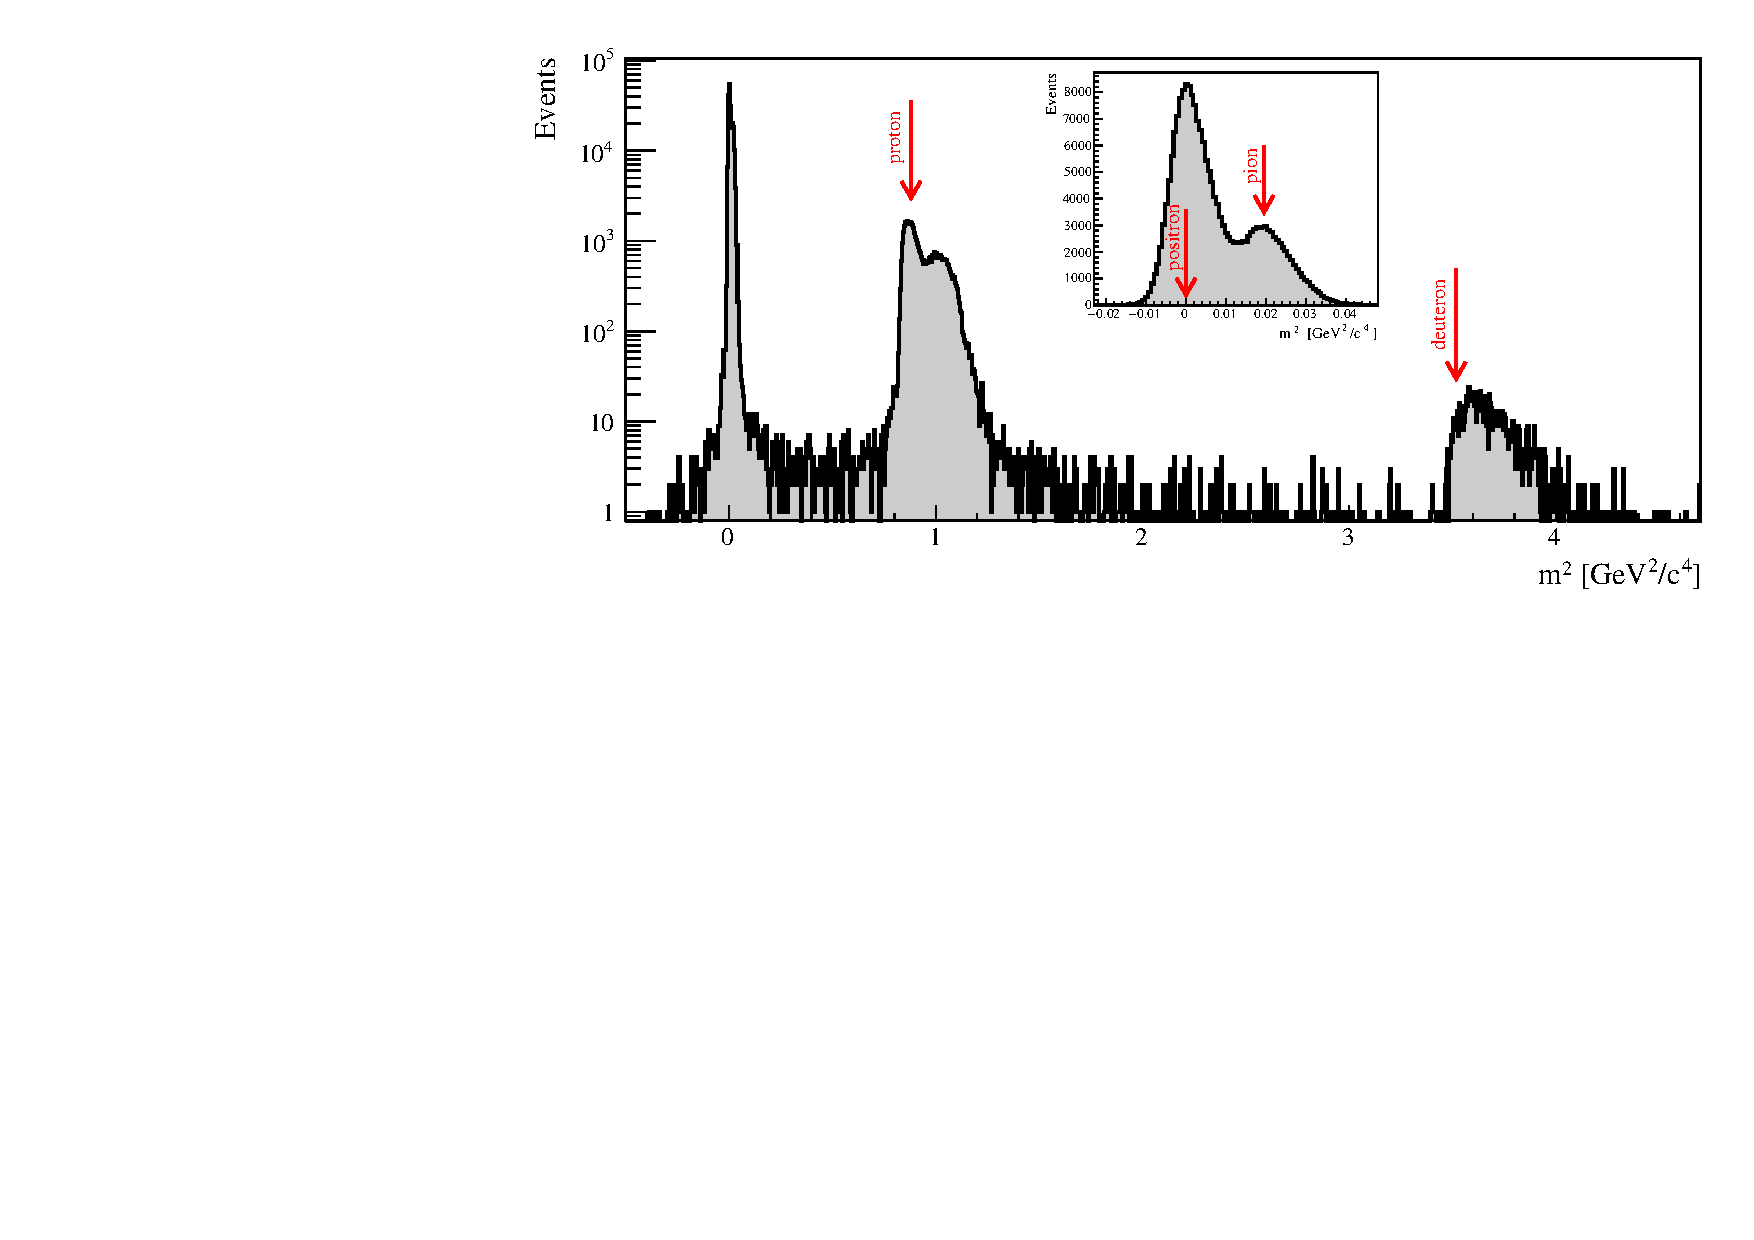
\includegraphics[width=0.9\linewidth]{files/Figures/Data_2018_8_31_b2_800MeV_0block_All.pdf}
	\caption{Reconstructed mass spectrum for the data taken without moderator blocks. The spectrum was calculated using the time difference between $\mathit{S3}$ and $\mathit{S1}$. Vertical arrows show predicted position of particles.}
	\label{fig:s3tof_mass}
\end{figure}

For the data collected in $\mathit{S3}$, both timing and signal amplitude cuts were used to select protons and MIPs.
Figure~\ref{fig:TvsA} shows an example of the signal size recorded in one of the SiPMs on one of the scintillator bars against the measured value of $t_{\mathit{S3}} - t_{\mathit{S1}}$.
At the beam energies used, due to their higher mass, the protons typically deposit more energy in the detector, resulting in the observation of greater amplitudes.
Therefore, to reduce the number of background events in the proton sample, a minimum signal amplitude is required.
This cut varies, depending on the SiPM in question and is determined from distributions such as those shown in Figure~\ref{fig:TvsA}. 
The cut values vary in the range 0.125~V to 0.3~V.

\begin{figure}[h]
  \begin{minipage}[t]{0.49\textwidth}
    \begin{adjustbox}{max totalsize={\textwidth}, center}
      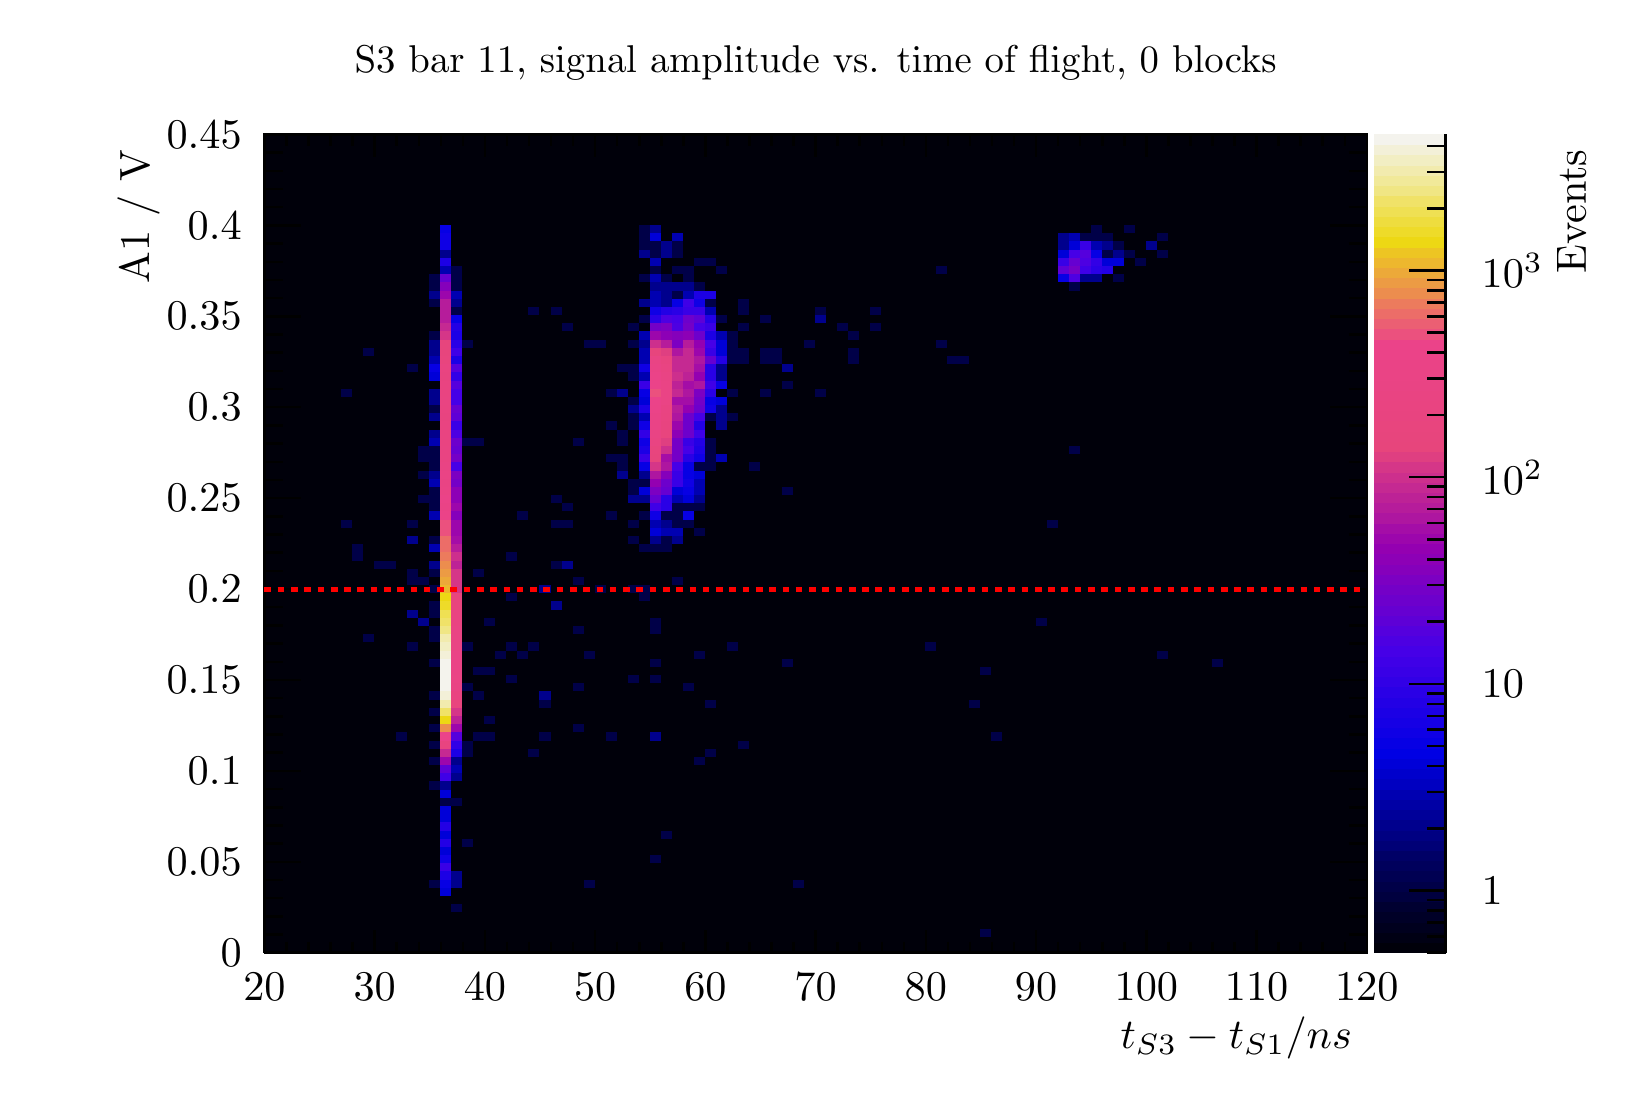
\begin{tikzpicture}
\pgfdeclareplotmark{cross} {
\pgfpathmoveto{\pgfpoint{-0.3\pgfplotmarksize}{\pgfplotmarksize}}
\pgfpathlineto{\pgfpoint{+0.3\pgfplotmarksize}{\pgfplotmarksize}}
\pgfpathlineto{\pgfpoint{+0.3\pgfplotmarksize}{0.3\pgfplotmarksize}}
\pgfpathlineto{\pgfpoint{+1\pgfplotmarksize}{0.3\pgfplotmarksize}}
\pgfpathlineto{\pgfpoint{+1\pgfplotmarksize}{-0.3\pgfplotmarksize}}
\pgfpathlineto{\pgfpoint{+0.3\pgfplotmarksize}{-0.3\pgfplotmarksize}}
\pgfpathlineto{\pgfpoint{+0.3\pgfplotmarksize}{-1.\pgfplotmarksize}}
\pgfpathlineto{\pgfpoint{-0.3\pgfplotmarksize}{-1.\pgfplotmarksize}}
\pgfpathlineto{\pgfpoint{-0.3\pgfplotmarksize}{-0.3\pgfplotmarksize}}
\pgfpathlineto{\pgfpoint{-1.\pgfplotmarksize}{-0.3\pgfplotmarksize}}
\pgfpathlineto{\pgfpoint{-1.\pgfplotmarksize}{0.3\pgfplotmarksize}}
\pgfpathlineto{\pgfpoint{-0.3\pgfplotmarksize}{0.3\pgfplotmarksize}}
\pgfpathclose
\pgfusepathqstroke
}
\pgfdeclareplotmark{cross*} {
\pgfpathmoveto{\pgfpoint{-0.3\pgfplotmarksize}{\pgfplotmarksize}}
\pgfpathlineto{\pgfpoint{+0.3\pgfplotmarksize}{\pgfplotmarksize}}
\pgfpathlineto{\pgfpoint{+0.3\pgfplotmarksize}{0.3\pgfplotmarksize}}
\pgfpathlineto{\pgfpoint{+1\pgfplotmarksize}{0.3\pgfplotmarksize}}
\pgfpathlineto{\pgfpoint{+1\pgfplotmarksize}{-0.3\pgfplotmarksize}}
\pgfpathlineto{\pgfpoint{+0.3\pgfplotmarksize}{-0.3\pgfplotmarksize}}
\pgfpathlineto{\pgfpoint{+0.3\pgfplotmarksize}{-1.\pgfplotmarksize}}
\pgfpathlineto{\pgfpoint{-0.3\pgfplotmarksize}{-1.\pgfplotmarksize}}
\pgfpathlineto{\pgfpoint{-0.3\pgfplotmarksize}{-0.3\pgfplotmarksize}}
\pgfpathlineto{\pgfpoint{-1.\pgfplotmarksize}{-0.3\pgfplotmarksize}}
\pgfpathlineto{\pgfpoint{-1.\pgfplotmarksize}{0.3\pgfplotmarksize}}
\pgfpathlineto{\pgfpoint{-0.3\pgfplotmarksize}{0.3\pgfplotmarksize}}
\pgfpathclose
\pgfusepathqfillstroke
}
\pgfdeclareplotmark{newstar} {
\pgfpathmoveto{\pgfqpoint{0pt}{\pgfplotmarksize}}
\pgfpathlineto{\pgfqpointpolar{44}{0.5\pgfplotmarksize}}
\pgfpathlineto{\pgfqpointpolar{18}{\pgfplotmarksize}}
\pgfpathlineto{\pgfqpointpolar{-20}{0.5\pgfplotmarksize}}
\pgfpathlineto{\pgfqpointpolar{-54}{\pgfplotmarksize}}
\pgfpathlineto{\pgfqpointpolar{-90}{0.5\pgfplotmarksize}}
\pgfpathlineto{\pgfqpointpolar{234}{\pgfplotmarksize}}
\pgfpathlineto{\pgfqpointpolar{198}{0.5\pgfplotmarksize}}
\pgfpathlineto{\pgfqpointpolar{162}{\pgfplotmarksize}}
\pgfpathlineto{\pgfqpointpolar{134}{0.5\pgfplotmarksize}}
\pgfpathclose
\pgfusepathqstroke
}
\pgfdeclareplotmark{newstar*} {
\pgfpathmoveto{\pgfqpoint{0pt}{\pgfplotmarksize}}
\pgfpathlineto{\pgfqpointpolar{44}{0.5\pgfplotmarksize}}
\pgfpathlineto{\pgfqpointpolar{18}{\pgfplotmarksize}}
\pgfpathlineto{\pgfqpointpolar{-20}{0.5\pgfplotmarksize}}
\pgfpathlineto{\pgfqpointpolar{-54}{\pgfplotmarksize}}
\pgfpathlineto{\pgfqpointpolar{-90}{0.5\pgfplotmarksize}}
\pgfpathlineto{\pgfqpointpolar{234}{\pgfplotmarksize}}
\pgfpathlineto{\pgfqpointpolar{198}{0.5\pgfplotmarksize}}
\pgfpathlineto{\pgfqpointpolar{162}{\pgfplotmarksize}}
\pgfpathlineto{\pgfqpointpolar{134}{0.5\pgfplotmarksize}}
\pgfpathclose
\pgfusepathqfillstroke
}
\definecolor{c}{rgb}{1,1,1};
\draw [color=c, fill=c] (0,0) rectangle (20,13.4957);
\draw [color=c, fill=c] (3,1.75444) rectangle (17,12.1461);
\definecolor{c}{rgb}{0,0,0};
\draw [c,line width=0.9] (3,1.75444) -- (3,12.1461) -- (17,12.1461) -- (17,1.75444) -- (3,1.75444);
\definecolor{c}{rgb}{1,1,1};
\draw [color=c, fill=c] (3,1.75444) rectangle (17,12.1461);
\definecolor{c}{rgb}{0,0,0};
\draw [c,line width=0.9] (3,1.75444) -- (3,12.1461) -- (17,12.1461) -- (17,1.75444) -- (3,1.75444);
\definecolor{c}{rgb}{0,0,0.0387097};
\draw [color=c, fill=c] (3,1.75444) rectangle (3.14,1.85836);
\draw [color=c, fill=c] (3.14,1.75444) rectangle (3.28,1.85836);
\draw [color=c, fill=c] (3.28,1.75444) rectangle (3.42,1.85836);
\draw [color=c, fill=c] (3.42,1.75444) rectangle (3.56,1.85836);
\draw [color=c, fill=c] (3.56,1.75444) rectangle (3.7,1.85836);
\draw [color=c, fill=c] (3.7,1.75444) rectangle (3.84,1.85836);
\draw [color=c, fill=c] (3.84,1.75444) rectangle (3.98,1.85836);
\draw [color=c, fill=c] (3.98,1.75444) rectangle (4.12,1.85836);
\draw [color=c, fill=c] (4.12,1.75444) rectangle (4.26,1.85836);
\draw [color=c, fill=c] (4.26,1.75444) rectangle (4.4,1.85836);
\draw [color=c, fill=c] (4.4,1.75444) rectangle (4.54,1.85836);
\draw [color=c, fill=c] (4.54,1.75444) rectangle (4.68,1.85836);
\draw [color=c, fill=c] (4.68,1.75444) rectangle (4.82,1.85836);
\draw [color=c, fill=c] (4.82,1.75444) rectangle (4.96,1.85836);
\draw [color=c, fill=c] (4.96,1.75444) rectangle (5.1,1.85836);
\draw [color=c, fill=c] (5.1,1.75444) rectangle (5.24,1.85836);
\draw [color=c, fill=c] (5.24,1.75444) rectangle (5.38,1.85836);
\draw [color=c, fill=c] (5.38,1.75444) rectangle (5.52,1.85836);
\draw [color=c, fill=c] (5.52,1.75444) rectangle (5.66,1.85836);
\draw [color=c, fill=c] (5.66,1.75444) rectangle (5.8,1.85836);
\draw [color=c, fill=c] (5.8,1.75444) rectangle (5.94,1.85836);
\draw [color=c, fill=c] (5.94,1.75444) rectangle (6.08,1.85836);
\draw [color=c, fill=c] (6.08,1.75444) rectangle (6.22,1.85836);
\draw [color=c, fill=c] (6.22,1.75444) rectangle (6.36,1.85836);
\draw [color=c, fill=c] (6.36,1.75444) rectangle (6.5,1.85836);
\draw [color=c, fill=c] (6.5,1.75444) rectangle (6.64,1.85836);
\draw [color=c, fill=c] (6.64,1.75444) rectangle (6.78,1.85836);
\draw [color=c, fill=c] (6.78,1.75444) rectangle (6.92,1.85836);
\draw [color=c, fill=c] (6.92,1.75444) rectangle (7.06,1.85836);
\draw [color=c, fill=c] (7.06,1.75444) rectangle (7.2,1.85836);
\draw [color=c, fill=c] (7.2,1.75444) rectangle (7.34,1.85836);
\draw [color=c, fill=c] (7.34,1.75444) rectangle (7.48,1.85836);
\draw [color=c, fill=c] (7.48,1.75444) rectangle (7.62,1.85836);
\draw [color=c, fill=c] (7.62,1.75444) rectangle (7.76,1.85836);
\draw [color=c, fill=c] (7.76,1.75444) rectangle (7.9,1.85836);
\draw [color=c, fill=c] (7.9,1.75444) rectangle (8.04,1.85836);
\draw [color=c, fill=c] (8.04,1.75444) rectangle (8.18,1.85836);
\draw [color=c, fill=c] (8.18,1.75444) rectangle (8.32,1.85836);
\draw [color=c, fill=c] (8.32,1.75444) rectangle (8.46,1.85836);
\draw [color=c, fill=c] (8.46,1.75444) rectangle (8.6,1.85836);
\draw [color=c, fill=c] (8.6,1.75444) rectangle (8.74,1.85836);
\draw [color=c, fill=c] (8.74,1.75444) rectangle (8.88,1.85836);
\draw [color=c, fill=c] (8.88,1.75444) rectangle (9.02,1.85836);
\draw [color=c, fill=c] (9.02,1.75444) rectangle (9.16,1.85836);
\draw [color=c, fill=c] (9.16,1.75444) rectangle (9.3,1.85836);
\draw [color=c, fill=c] (9.3,1.75444) rectangle (9.44,1.85836);
\draw [color=c, fill=c] (9.44,1.75444) rectangle (9.58,1.85836);
\draw [color=c, fill=c] (9.58,1.75444) rectangle (9.72,1.85836);
\draw [color=c, fill=c] (9.72,1.75444) rectangle (9.86,1.85836);
\draw [color=c, fill=c] (9.86,1.75444) rectangle (10,1.85836);
\draw [color=c, fill=c] (10,1.75444) rectangle (10.14,1.85836);
\draw [color=c, fill=c] (10.14,1.75444) rectangle (10.28,1.85836);
\draw [color=c, fill=c] (10.28,1.75444) rectangle (10.42,1.85836);
\draw [color=c, fill=c] (10.42,1.75444) rectangle (10.56,1.85836);
\draw [color=c, fill=c] (10.56,1.75444) rectangle (10.7,1.85836);
\draw [color=c, fill=c] (10.7,1.75444) rectangle (10.84,1.85836);
\draw [color=c, fill=c] (10.84,1.75444) rectangle (10.98,1.85836);
\draw [color=c, fill=c] (10.98,1.75444) rectangle (11.12,1.85836);
\draw [color=c, fill=c] (11.12,1.75444) rectangle (11.26,1.85836);
\draw [color=c, fill=c] (11.26,1.75444) rectangle (11.4,1.85836);
\draw [color=c, fill=c] (11.4,1.75444) rectangle (11.54,1.85836);
\draw [color=c, fill=c] (11.54,1.75444) rectangle (11.68,1.85836);
\draw [color=c, fill=c] (11.68,1.75444) rectangle (11.82,1.85836);
\draw [color=c, fill=c] (11.82,1.75444) rectangle (11.96,1.85836);
\draw [color=c, fill=c] (11.96,1.75444) rectangle (12.1,1.85836);
\draw [color=c, fill=c] (12.1,1.75444) rectangle (12.24,1.85836);
\draw [color=c, fill=c] (12.24,1.75444) rectangle (12.38,1.85836);
\draw [color=c, fill=c] (12.38,1.75444) rectangle (12.52,1.85836);
\draw [color=c, fill=c] (12.52,1.75444) rectangle (12.66,1.85836);
\draw [color=c, fill=c] (12.66,1.75444) rectangle (12.8,1.85836);
\draw [color=c, fill=c] (12.8,1.75444) rectangle (12.94,1.85836);
\draw [color=c, fill=c] (12.94,1.75444) rectangle (13.08,1.85836);
\draw [color=c, fill=c] (13.08,1.75444) rectangle (13.22,1.85836);
\draw [color=c, fill=c] (13.22,1.75444) rectangle (13.36,1.85836);
\draw [color=c, fill=c] (13.36,1.75444) rectangle (13.5,1.85836);
\draw [color=c, fill=c] (13.5,1.75444) rectangle (13.64,1.85836);
\draw [color=c, fill=c] (13.64,1.75444) rectangle (13.78,1.85836);
\draw [color=c, fill=c] (13.78,1.75444) rectangle (13.92,1.85836);
\draw [color=c, fill=c] (13.92,1.75444) rectangle (14.06,1.85836);
\draw [color=c, fill=c] (14.06,1.75444) rectangle (14.2,1.85836);
\draw [color=c, fill=c] (14.2,1.75444) rectangle (14.34,1.85836);
\draw [color=c, fill=c] (14.34,1.75444) rectangle (14.48,1.85836);
\draw [color=c, fill=c] (14.48,1.75444) rectangle (14.62,1.85836);
\draw [color=c, fill=c] (14.62,1.75444) rectangle (14.76,1.85836);
\draw [color=c, fill=c] (14.76,1.75444) rectangle (14.9,1.85836);
\draw [color=c, fill=c] (14.9,1.75444) rectangle (15.04,1.85836);
\draw [color=c, fill=c] (15.04,1.75444) rectangle (15.18,1.85836);
\draw [color=c, fill=c] (15.18,1.75444) rectangle (15.32,1.85836);
\draw [color=c, fill=c] (15.32,1.75444) rectangle (15.46,1.85836);
\draw [color=c, fill=c] (15.46,1.75444) rectangle (15.6,1.85836);
\draw [color=c, fill=c] (15.6,1.75444) rectangle (15.74,1.85836);
\draw [color=c, fill=c] (15.74,1.75444) rectangle (15.88,1.85836);
\draw [color=c, fill=c] (15.88,1.75444) rectangle (16.02,1.85836);
\draw [color=c, fill=c] (16.02,1.75444) rectangle (16.16,1.85836);
\draw [color=c, fill=c] (16.16,1.75444) rectangle (16.3,1.85836);
\draw [color=c, fill=c] (16.3,1.75444) rectangle (16.44,1.85836);
\draw [color=c, fill=c] (16.44,1.75444) rectangle (16.58,1.85836);
\draw [color=c, fill=c] (16.58,1.75444) rectangle (16.72,1.85836);
\draw [color=c, fill=c] (16.72,1.75444) rectangle (16.86,1.85836);
\draw [color=c, fill=c] (16.86,1.75444) rectangle (17,1.85836);
\draw [color=c, fill=c] (3,1.85836) rectangle (3.14,1.96228);
\draw [color=c, fill=c] (3.14,1.85836) rectangle (3.28,1.96228);
\draw [color=c, fill=c] (3.28,1.85836) rectangle (3.42,1.96228);
\draw [color=c, fill=c] (3.42,1.85836) rectangle (3.56,1.96228);
\draw [color=c, fill=c] (3.56,1.85836) rectangle (3.7,1.96228);
\draw [color=c, fill=c] (3.7,1.85836) rectangle (3.84,1.96228);
\draw [color=c, fill=c] (3.84,1.85836) rectangle (3.98,1.96228);
\draw [color=c, fill=c] (3.98,1.85836) rectangle (4.12,1.96228);
\draw [color=c, fill=c] (4.12,1.85836) rectangle (4.26,1.96228);
\draw [color=c, fill=c] (4.26,1.85836) rectangle (4.4,1.96228);
\draw [color=c, fill=c] (4.4,1.85836) rectangle (4.54,1.96228);
\draw [color=c, fill=c] (4.54,1.85836) rectangle (4.68,1.96228);
\draw [color=c, fill=c] (4.68,1.85836) rectangle (4.82,1.96228);
\draw [color=c, fill=c] (4.82,1.85836) rectangle (4.96,1.96228);
\draw [color=c, fill=c] (4.96,1.85836) rectangle (5.1,1.96228);
\draw [color=c, fill=c] (5.1,1.85836) rectangle (5.24,1.96228);
\draw [color=c, fill=c] (5.24,1.85836) rectangle (5.38,1.96228);
\draw [color=c, fill=c] (5.38,1.85836) rectangle (5.52,1.96228);
\draw [color=c, fill=c] (5.52,1.85836) rectangle (5.66,1.96228);
\draw [color=c, fill=c] (5.66,1.85836) rectangle (5.8,1.96228);
\draw [color=c, fill=c] (5.8,1.85836) rectangle (5.94,1.96228);
\draw [color=c, fill=c] (5.94,1.85836) rectangle (6.08,1.96228);
\draw [color=c, fill=c] (6.08,1.85836) rectangle (6.22,1.96228);
\draw [color=c, fill=c] (6.22,1.85836) rectangle (6.36,1.96228);
\draw [color=c, fill=c] (6.36,1.85836) rectangle (6.5,1.96228);
\draw [color=c, fill=c] (6.5,1.85836) rectangle (6.64,1.96228);
\draw [color=c, fill=c] (6.64,1.85836) rectangle (6.78,1.96228);
\draw [color=c, fill=c] (6.78,1.85836) rectangle (6.92,1.96228);
\draw [color=c, fill=c] (6.92,1.85836) rectangle (7.06,1.96228);
\draw [color=c, fill=c] (7.06,1.85836) rectangle (7.2,1.96228);
\draw [color=c, fill=c] (7.2,1.85836) rectangle (7.34,1.96228);
\draw [color=c, fill=c] (7.34,1.85836) rectangle (7.48,1.96228);
\draw [color=c, fill=c] (7.48,1.85836) rectangle (7.62,1.96228);
\draw [color=c, fill=c] (7.62,1.85836) rectangle (7.76,1.96228);
\draw [color=c, fill=c] (7.76,1.85836) rectangle (7.9,1.96228);
\draw [color=c, fill=c] (7.9,1.85836) rectangle (8.04,1.96228);
\draw [color=c, fill=c] (8.04,1.85836) rectangle (8.18,1.96228);
\draw [color=c, fill=c] (8.18,1.85836) rectangle (8.32,1.96228);
\draw [color=c, fill=c] (8.32,1.85836) rectangle (8.46,1.96228);
\draw [color=c, fill=c] (8.46,1.85836) rectangle (8.6,1.96228);
\draw [color=c, fill=c] (8.6,1.85836) rectangle (8.74,1.96228);
\draw [color=c, fill=c] (8.74,1.85836) rectangle (8.88,1.96228);
\draw [color=c, fill=c] (8.88,1.85836) rectangle (9.02,1.96228);
\draw [color=c, fill=c] (9.02,1.85836) rectangle (9.16,1.96228);
\draw [color=c, fill=c] (9.16,1.85836) rectangle (9.3,1.96228);
\draw [color=c, fill=c] (9.3,1.85836) rectangle (9.44,1.96228);
\draw [color=c, fill=c] (9.44,1.85836) rectangle (9.58,1.96228);
\draw [color=c, fill=c] (9.58,1.85836) rectangle (9.72,1.96228);
\draw [color=c, fill=c] (9.72,1.85836) rectangle (9.86,1.96228);
\draw [color=c, fill=c] (9.86,1.85836) rectangle (10,1.96228);
\draw [color=c, fill=c] (10,1.85836) rectangle (10.14,1.96228);
\draw [color=c, fill=c] (10.14,1.85836) rectangle (10.28,1.96228);
\draw [color=c, fill=c] (10.28,1.85836) rectangle (10.42,1.96228);
\draw [color=c, fill=c] (10.42,1.85836) rectangle (10.56,1.96228);
\draw [color=c, fill=c] (10.56,1.85836) rectangle (10.7,1.96228);
\draw [color=c, fill=c] (10.7,1.85836) rectangle (10.84,1.96228);
\draw [color=c, fill=c] (10.84,1.85836) rectangle (10.98,1.96228);
\draw [color=c, fill=c] (10.98,1.85836) rectangle (11.12,1.96228);
\draw [color=c, fill=c] (11.12,1.85836) rectangle (11.26,1.96228);
\draw [color=c, fill=c] (11.26,1.85836) rectangle (11.4,1.96228);
\draw [color=c, fill=c] (11.4,1.85836) rectangle (11.54,1.96228);
\draw [color=c, fill=c] (11.54,1.85836) rectangle (11.68,1.96228);
\draw [color=c, fill=c] (11.68,1.85836) rectangle (11.82,1.96228);
\draw [color=c, fill=c] (11.82,1.85836) rectangle (11.96,1.96228);
\draw [color=c, fill=c] (11.96,1.85836) rectangle (12.1,1.96228);
\draw [color=c, fill=c] (12.1,1.85836) rectangle (12.24,1.96228);
\draw [color=c, fill=c] (12.24,1.85836) rectangle (12.38,1.96228);
\draw [color=c, fill=c] (12.38,1.85836) rectangle (12.52,1.96228);
\draw [color=c, fill=c] (12.52,1.85836) rectangle (12.66,1.96228);
\draw [color=c, fill=c] (12.66,1.85836) rectangle (12.8,1.96228);
\draw [color=c, fill=c] (12.8,1.85836) rectangle (12.94,1.96228);
\draw [color=c, fill=c] (12.94,1.85836) rectangle (13.08,1.96228);
\draw [color=c, fill=c] (13.08,1.85836) rectangle (13.22,1.96228);
\draw [color=c, fill=c] (13.22,1.85836) rectangle (13.36,1.96228);
\draw [color=c, fill=c] (13.36,1.85836) rectangle (13.5,1.96228);
\draw [color=c, fill=c] (13.5,1.85836) rectangle (13.64,1.96228);
\draw [color=c, fill=c] (13.64,1.85836) rectangle (13.78,1.96228);
\draw [color=c, fill=c] (13.78,1.85836) rectangle (13.92,1.96228);
\draw [color=c, fill=c] (13.92,1.85836) rectangle (14.06,1.96228);
\draw [color=c, fill=c] (14.06,1.85836) rectangle (14.2,1.96228);
\draw [color=c, fill=c] (14.2,1.85836) rectangle (14.34,1.96228);
\draw [color=c, fill=c] (14.34,1.85836) rectangle (14.48,1.96228);
\draw [color=c, fill=c] (14.48,1.85836) rectangle (14.62,1.96228);
\draw [color=c, fill=c] (14.62,1.85836) rectangle (14.76,1.96228);
\draw [color=c, fill=c] (14.76,1.85836) rectangle (14.9,1.96228);
\draw [color=c, fill=c] (14.9,1.85836) rectangle (15.04,1.96228);
\draw [color=c, fill=c] (15.04,1.85836) rectangle (15.18,1.96228);
\draw [color=c, fill=c] (15.18,1.85836) rectangle (15.32,1.96228);
\draw [color=c, fill=c] (15.32,1.85836) rectangle (15.46,1.96228);
\draw [color=c, fill=c] (15.46,1.85836) rectangle (15.6,1.96228);
\draw [color=c, fill=c] (15.6,1.85836) rectangle (15.74,1.96228);
\draw [color=c, fill=c] (15.74,1.85836) rectangle (15.88,1.96228);
\draw [color=c, fill=c] (15.88,1.85836) rectangle (16.02,1.96228);
\draw [color=c, fill=c] (16.02,1.85836) rectangle (16.16,1.96228);
\draw [color=c, fill=c] (16.16,1.85836) rectangle (16.3,1.96228);
\draw [color=c, fill=c] (16.3,1.85836) rectangle (16.44,1.96228);
\draw [color=c, fill=c] (16.44,1.85836) rectangle (16.58,1.96228);
\draw [color=c, fill=c] (16.58,1.85836) rectangle (16.72,1.96228);
\draw [color=c, fill=c] (16.72,1.85836) rectangle (16.86,1.96228);
\draw [color=c, fill=c] (16.86,1.85836) rectangle (17,1.96228);
\draw [color=c, fill=c] (3,1.96228) rectangle (3.14,2.06619);
\draw [color=c, fill=c] (3.14,1.96228) rectangle (3.28,2.06619);
\draw [color=c, fill=c] (3.28,1.96228) rectangle (3.42,2.06619);
\draw [color=c, fill=c] (3.42,1.96228) rectangle (3.56,2.06619);
\draw [color=c, fill=c] (3.56,1.96228) rectangle (3.7,2.06619);
\draw [color=c, fill=c] (3.7,1.96228) rectangle (3.84,2.06619);
\draw [color=c, fill=c] (3.84,1.96228) rectangle (3.98,2.06619);
\draw [color=c, fill=c] (3.98,1.96228) rectangle (4.12,2.06619);
\draw [color=c, fill=c] (4.12,1.96228) rectangle (4.26,2.06619);
\draw [color=c, fill=c] (4.26,1.96228) rectangle (4.4,2.06619);
\draw [color=c, fill=c] (4.4,1.96228) rectangle (4.54,2.06619);
\draw [color=c, fill=c] (4.54,1.96228) rectangle (4.68,2.06619);
\draw [color=c, fill=c] (4.68,1.96228) rectangle (4.82,2.06619);
\draw [color=c, fill=c] (4.82,1.96228) rectangle (4.96,2.06619);
\draw [color=c, fill=c] (4.96,1.96228) rectangle (5.1,2.06619);
\draw [color=c, fill=c] (5.1,1.96228) rectangle (5.24,2.06619);
\draw [color=c, fill=c] (5.24,1.96228) rectangle (5.38,2.06619);
\draw [color=c, fill=c] (5.38,1.96228) rectangle (5.52,2.06619);
\draw [color=c, fill=c] (5.52,1.96228) rectangle (5.66,2.06619);
\draw [color=c, fill=c] (5.66,1.96228) rectangle (5.8,2.06619);
\draw [color=c, fill=c] (5.8,1.96228) rectangle (5.94,2.06619);
\draw [color=c, fill=c] (5.94,1.96228) rectangle (6.08,2.06619);
\draw [color=c, fill=c] (6.08,1.96228) rectangle (6.22,2.06619);
\draw [color=c, fill=c] (6.22,1.96228) rectangle (6.36,2.06619);
\draw [color=c, fill=c] (6.36,1.96228) rectangle (6.5,2.06619);
\draw [color=c, fill=c] (6.5,1.96228) rectangle (6.64,2.06619);
\draw [color=c, fill=c] (6.64,1.96228) rectangle (6.78,2.06619);
\draw [color=c, fill=c] (6.78,1.96228) rectangle (6.92,2.06619);
\draw [color=c, fill=c] (6.92,1.96228) rectangle (7.06,2.06619);
\draw [color=c, fill=c] (7.06,1.96228) rectangle (7.2,2.06619);
\draw [color=c, fill=c] (7.2,1.96228) rectangle (7.34,2.06619);
\draw [color=c, fill=c] (7.34,1.96228) rectangle (7.48,2.06619);
\draw [color=c, fill=c] (7.48,1.96228) rectangle (7.62,2.06619);
\draw [color=c, fill=c] (7.62,1.96228) rectangle (7.76,2.06619);
\draw [color=c, fill=c] (7.76,1.96228) rectangle (7.9,2.06619);
\draw [color=c, fill=c] (7.9,1.96228) rectangle (8.04,2.06619);
\draw [color=c, fill=c] (8.04,1.96228) rectangle (8.18,2.06619);
\draw [color=c, fill=c] (8.18,1.96228) rectangle (8.32,2.06619);
\draw [color=c, fill=c] (8.32,1.96228) rectangle (8.46,2.06619);
\draw [color=c, fill=c] (8.46,1.96228) rectangle (8.6,2.06619);
\draw [color=c, fill=c] (8.6,1.96228) rectangle (8.74,2.06619);
\draw [color=c, fill=c] (8.74,1.96228) rectangle (8.88,2.06619);
\draw [color=c, fill=c] (8.88,1.96228) rectangle (9.02,2.06619);
\draw [color=c, fill=c] (9.02,1.96228) rectangle (9.16,2.06619);
\draw [color=c, fill=c] (9.16,1.96228) rectangle (9.3,2.06619);
\draw [color=c, fill=c] (9.3,1.96228) rectangle (9.44,2.06619);
\draw [color=c, fill=c] (9.44,1.96228) rectangle (9.58,2.06619);
\draw [color=c, fill=c] (9.58,1.96228) rectangle (9.72,2.06619);
\draw [color=c, fill=c] (9.72,1.96228) rectangle (9.86,2.06619);
\draw [color=c, fill=c] (9.86,1.96228) rectangle (10,2.06619);
\draw [color=c, fill=c] (10,1.96228) rectangle (10.14,2.06619);
\draw [color=c, fill=c] (10.14,1.96228) rectangle (10.28,2.06619);
\draw [color=c, fill=c] (10.28,1.96228) rectangle (10.42,2.06619);
\draw [color=c, fill=c] (10.42,1.96228) rectangle (10.56,2.06619);
\draw [color=c, fill=c] (10.56,1.96228) rectangle (10.7,2.06619);
\draw [color=c, fill=c] (10.7,1.96228) rectangle (10.84,2.06619);
\draw [color=c, fill=c] (10.84,1.96228) rectangle (10.98,2.06619);
\draw [color=c, fill=c] (10.98,1.96228) rectangle (11.12,2.06619);
\draw [color=c, fill=c] (11.12,1.96228) rectangle (11.26,2.06619);
\draw [color=c, fill=c] (11.26,1.96228) rectangle (11.4,2.06619);
\draw [color=c, fill=c] (11.4,1.96228) rectangle (11.54,2.06619);
\draw [color=c, fill=c] (11.54,1.96228) rectangle (11.68,2.06619);
\draw [color=c, fill=c] (11.68,1.96228) rectangle (11.82,2.06619);
\draw [color=c, fill=c] (11.82,1.96228) rectangle (11.96,2.06619);
\draw [color=c, fill=c] (11.96,1.96228) rectangle (12.1,2.06619);
\definecolor{c}{rgb}{0,0,0.283871};
\draw [color=c, fill=c] (12.1,1.96228) rectangle (12.24,2.06619);
\definecolor{c}{rgb}{0,0,0.0387097};
\draw [color=c, fill=c] (12.24,1.96228) rectangle (12.38,2.06619);
\draw [color=c, fill=c] (12.38,1.96228) rectangle (12.52,2.06619);
\draw [color=c, fill=c] (12.52,1.96228) rectangle (12.66,2.06619);
\draw [color=c, fill=c] (12.66,1.96228) rectangle (12.8,2.06619);
\draw [color=c, fill=c] (12.8,1.96228) rectangle (12.94,2.06619);
\draw [color=c, fill=c] (12.94,1.96228) rectangle (13.08,2.06619);
\draw [color=c, fill=c] (13.08,1.96228) rectangle (13.22,2.06619);
\draw [color=c, fill=c] (13.22,1.96228) rectangle (13.36,2.06619);
\draw [color=c, fill=c] (13.36,1.96228) rectangle (13.5,2.06619);
\draw [color=c, fill=c] (13.5,1.96228) rectangle (13.64,2.06619);
\draw [color=c, fill=c] (13.64,1.96228) rectangle (13.78,2.06619);
\draw [color=c, fill=c] (13.78,1.96228) rectangle (13.92,2.06619);
\draw [color=c, fill=c] (13.92,1.96228) rectangle (14.06,2.06619);
\draw [color=c, fill=c] (14.06,1.96228) rectangle (14.2,2.06619);
\draw [color=c, fill=c] (14.2,1.96228) rectangle (14.34,2.06619);
\draw [color=c, fill=c] (14.34,1.96228) rectangle (14.48,2.06619);
\draw [color=c, fill=c] (14.48,1.96228) rectangle (14.62,2.06619);
\draw [color=c, fill=c] (14.62,1.96228) rectangle (14.76,2.06619);
\draw [color=c, fill=c] (14.76,1.96228) rectangle (14.9,2.06619);
\draw [color=c, fill=c] (14.9,1.96228) rectangle (15.04,2.06619);
\draw [color=c, fill=c] (15.04,1.96228) rectangle (15.18,2.06619);
\draw [color=c, fill=c] (15.18,1.96228) rectangle (15.32,2.06619);
\draw [color=c, fill=c] (15.32,1.96228) rectangle (15.46,2.06619);
\draw [color=c, fill=c] (15.46,1.96228) rectangle (15.6,2.06619);
\draw [color=c, fill=c] (15.6,1.96228) rectangle (15.74,2.06619);
\draw [color=c, fill=c] (15.74,1.96228) rectangle (15.88,2.06619);
\draw [color=c, fill=c] (15.88,1.96228) rectangle (16.02,2.06619);
\draw [color=c, fill=c] (16.02,1.96228) rectangle (16.16,2.06619);
\draw [color=c, fill=c] (16.16,1.96228) rectangle (16.3,2.06619);
\draw [color=c, fill=c] (16.3,1.96228) rectangle (16.44,2.06619);
\draw [color=c, fill=c] (16.44,1.96228) rectangle (16.58,2.06619);
\draw [color=c, fill=c] (16.58,1.96228) rectangle (16.72,2.06619);
\draw [color=c, fill=c] (16.72,1.96228) rectangle (16.86,2.06619);
\draw [color=c, fill=c] (16.86,1.96228) rectangle (17,2.06619);
\draw [color=c, fill=c] (3,2.06619) rectangle (3.14,2.17011);
\draw [color=c, fill=c] (3.14,2.06619) rectangle (3.28,2.17011);
\draw [color=c, fill=c] (3.28,2.06619) rectangle (3.42,2.17011);
\draw [color=c, fill=c] (3.42,2.06619) rectangle (3.56,2.17011);
\draw [color=c, fill=c] (3.56,2.06619) rectangle (3.7,2.17011);
\draw [color=c, fill=c] (3.7,2.06619) rectangle (3.84,2.17011);
\draw [color=c, fill=c] (3.84,2.06619) rectangle (3.98,2.17011);
\draw [color=c, fill=c] (3.98,2.06619) rectangle (4.12,2.17011);
\draw [color=c, fill=c] (4.12,2.06619) rectangle (4.26,2.17011);
\draw [color=c, fill=c] (4.26,2.06619) rectangle (4.4,2.17011);
\draw [color=c, fill=c] (4.4,2.06619) rectangle (4.54,2.17011);
\draw [color=c, fill=c] (4.54,2.06619) rectangle (4.68,2.17011);
\draw [color=c, fill=c] (4.68,2.06619) rectangle (4.82,2.17011);
\draw [color=c, fill=c] (4.82,2.06619) rectangle (4.96,2.17011);
\draw [color=c, fill=c] (4.96,2.06619) rectangle (5.1,2.17011);
\draw [color=c, fill=c] (5.1,2.06619) rectangle (5.24,2.17011);
\draw [color=c, fill=c] (5.24,2.06619) rectangle (5.38,2.17011);
\draw [color=c, fill=c] (5.38,2.06619) rectangle (5.52,2.17011);
\draw [color=c, fill=c] (5.52,2.06619) rectangle (5.66,2.17011);
\draw [color=c, fill=c] (5.66,2.06619) rectangle (5.8,2.17011);
\draw [color=c, fill=c] (5.8,2.06619) rectangle (5.94,2.17011);
\draw [color=c, fill=c] (5.94,2.06619) rectangle (6.08,2.17011);
\draw [color=c, fill=c] (6.08,2.06619) rectangle (6.22,2.17011);
\draw [color=c, fill=c] (6.22,2.06619) rectangle (6.36,2.17011);
\draw [color=c, fill=c] (6.36,2.06619) rectangle (6.5,2.17011);
\draw [color=c, fill=c] (6.5,2.06619) rectangle (6.64,2.17011);
\draw [color=c, fill=c] (6.64,2.06619) rectangle (6.78,2.17011);
\draw [color=c, fill=c] (6.78,2.06619) rectangle (6.92,2.17011);
\draw [color=c, fill=c] (6.92,2.06619) rectangle (7.06,2.17011);
\draw [color=c, fill=c] (7.06,2.06619) rectangle (7.2,2.17011);
\draw [color=c, fill=c] (7.2,2.06619) rectangle (7.34,2.17011);
\draw [color=c, fill=c] (7.34,2.06619) rectangle (7.48,2.17011);
\draw [color=c, fill=c] (7.48,2.06619) rectangle (7.62,2.17011);
\draw [color=c, fill=c] (7.62,2.06619) rectangle (7.76,2.17011);
\draw [color=c, fill=c] (7.76,2.06619) rectangle (7.9,2.17011);
\draw [color=c, fill=c] (7.9,2.06619) rectangle (8.04,2.17011);
\draw [color=c, fill=c] (8.04,2.06619) rectangle (8.18,2.17011);
\draw [color=c, fill=c] (8.18,2.06619) rectangle (8.32,2.17011);
\draw [color=c, fill=c] (8.32,2.06619) rectangle (8.46,2.17011);
\draw [color=c, fill=c] (8.46,2.06619) rectangle (8.6,2.17011);
\draw [color=c, fill=c] (8.6,2.06619) rectangle (8.74,2.17011);
\draw [color=c, fill=c] (8.74,2.06619) rectangle (8.88,2.17011);
\draw [color=c, fill=c] (8.88,2.06619) rectangle (9.02,2.17011);
\draw [color=c, fill=c] (9.02,2.06619) rectangle (9.16,2.17011);
\draw [color=c, fill=c] (9.16,2.06619) rectangle (9.3,2.17011);
\draw [color=c, fill=c] (9.3,2.06619) rectangle (9.44,2.17011);
\draw [color=c, fill=c] (9.44,2.06619) rectangle (9.58,2.17011);
\draw [color=c, fill=c] (9.58,2.06619) rectangle (9.72,2.17011);
\draw [color=c, fill=c] (9.72,2.06619) rectangle (9.86,2.17011);
\draw [color=c, fill=c] (9.86,2.06619) rectangle (10,2.17011);
\draw [color=c, fill=c] (10,2.06619) rectangle (10.14,2.17011);
\draw [color=c, fill=c] (10.14,2.06619) rectangle (10.28,2.17011);
\draw [color=c, fill=c] (10.28,2.06619) rectangle (10.42,2.17011);
\draw [color=c, fill=c] (10.42,2.06619) rectangle (10.56,2.17011);
\draw [color=c, fill=c] (10.56,2.06619) rectangle (10.7,2.17011);
\draw [color=c, fill=c] (10.7,2.06619) rectangle (10.84,2.17011);
\draw [color=c, fill=c] (10.84,2.06619) rectangle (10.98,2.17011);
\draw [color=c, fill=c] (10.98,2.06619) rectangle (11.12,2.17011);
\draw [color=c, fill=c] (11.12,2.06619) rectangle (11.26,2.17011);
\draw [color=c, fill=c] (11.26,2.06619) rectangle (11.4,2.17011);
\draw [color=c, fill=c] (11.4,2.06619) rectangle (11.54,2.17011);
\draw [color=c, fill=c] (11.54,2.06619) rectangle (11.68,2.17011);
\draw [color=c, fill=c] (11.68,2.06619) rectangle (11.82,2.17011);
\draw [color=c, fill=c] (11.82,2.06619) rectangle (11.96,2.17011);
\draw [color=c, fill=c] (11.96,2.06619) rectangle (12.1,2.17011);
\draw [color=c, fill=c] (12.1,2.06619) rectangle (12.24,2.17011);
\draw [color=c, fill=c] (12.24,2.06619) rectangle (12.38,2.17011);
\draw [color=c, fill=c] (12.38,2.06619) rectangle (12.52,2.17011);
\draw [color=c, fill=c] (12.52,2.06619) rectangle (12.66,2.17011);
\draw [color=c, fill=c] (12.66,2.06619) rectangle (12.8,2.17011);
\draw [color=c, fill=c] (12.8,2.06619) rectangle (12.94,2.17011);
\draw [color=c, fill=c] (12.94,2.06619) rectangle (13.08,2.17011);
\draw [color=c, fill=c] (13.08,2.06619) rectangle (13.22,2.17011);
\draw [color=c, fill=c] (13.22,2.06619) rectangle (13.36,2.17011);
\draw [color=c, fill=c] (13.36,2.06619) rectangle (13.5,2.17011);
\draw [color=c, fill=c] (13.5,2.06619) rectangle (13.64,2.17011);
\draw [color=c, fill=c] (13.64,2.06619) rectangle (13.78,2.17011);
\draw [color=c, fill=c] (13.78,2.06619) rectangle (13.92,2.17011);
\draw [color=c, fill=c] (13.92,2.06619) rectangle (14.06,2.17011);
\draw [color=c, fill=c] (14.06,2.06619) rectangle (14.2,2.17011);
\draw [color=c, fill=c] (14.2,2.06619) rectangle (14.34,2.17011);
\draw [color=c, fill=c] (14.34,2.06619) rectangle (14.48,2.17011);
\draw [color=c, fill=c] (14.48,2.06619) rectangle (14.62,2.17011);
\draw [color=c, fill=c] (14.62,2.06619) rectangle (14.76,2.17011);
\draw [color=c, fill=c] (14.76,2.06619) rectangle (14.9,2.17011);
\draw [color=c, fill=c] (14.9,2.06619) rectangle (15.04,2.17011);
\draw [color=c, fill=c] (15.04,2.06619) rectangle (15.18,2.17011);
\draw [color=c, fill=c] (15.18,2.06619) rectangle (15.32,2.17011);
\draw [color=c, fill=c] (15.32,2.06619) rectangle (15.46,2.17011);
\draw [color=c, fill=c] (15.46,2.06619) rectangle (15.6,2.17011);
\draw [color=c, fill=c] (15.6,2.06619) rectangle (15.74,2.17011);
\draw [color=c, fill=c] (15.74,2.06619) rectangle (15.88,2.17011);
\draw [color=c, fill=c] (15.88,2.06619) rectangle (16.02,2.17011);
\draw [color=c, fill=c] (16.02,2.06619) rectangle (16.16,2.17011);
\draw [color=c, fill=c] (16.16,2.06619) rectangle (16.3,2.17011);
\draw [color=c, fill=c] (16.3,2.06619) rectangle (16.44,2.17011);
\draw [color=c, fill=c] (16.44,2.06619) rectangle (16.58,2.17011);
\draw [color=c, fill=c] (16.58,2.06619) rectangle (16.72,2.17011);
\draw [color=c, fill=c] (16.72,2.06619) rectangle (16.86,2.17011);
\draw [color=c, fill=c] (16.86,2.06619) rectangle (17,2.17011);
\draw [color=c, fill=c] (3,2.17011) rectangle (3.14,2.27403);
\draw [color=c, fill=c] (3.14,2.17011) rectangle (3.28,2.27403);
\draw [color=c, fill=c] (3.28,2.17011) rectangle (3.42,2.27403);
\draw [color=c, fill=c] (3.42,2.17011) rectangle (3.56,2.27403);
\draw [color=c, fill=c] (3.56,2.17011) rectangle (3.7,2.27403);
\draw [color=c, fill=c] (3.7,2.17011) rectangle (3.84,2.27403);
\draw [color=c, fill=c] (3.84,2.17011) rectangle (3.98,2.27403);
\draw [color=c, fill=c] (3.98,2.17011) rectangle (4.12,2.27403);
\draw [color=c, fill=c] (4.12,2.17011) rectangle (4.26,2.27403);
\draw [color=c, fill=c] (4.26,2.17011) rectangle (4.4,2.27403);
\draw [color=c, fill=c] (4.4,2.17011) rectangle (4.54,2.27403);
\draw [color=c, fill=c] (4.54,2.17011) rectangle (4.68,2.27403);
\draw [color=c, fill=c] (4.68,2.17011) rectangle (4.82,2.27403);
\draw [color=c, fill=c] (4.82,2.17011) rectangle (4.96,2.27403);
\draw [color=c, fill=c] (4.96,2.17011) rectangle (5.1,2.27403);
\draw [color=c, fill=c] (5.1,2.17011) rectangle (5.24,2.27403);
\draw [color=c, fill=c] (5.24,2.17011) rectangle (5.38,2.27403);
\draw [color=c, fill=c] (5.38,2.17011) rectangle (5.52,2.27403);
\draw [color=c, fill=c] (5.52,2.17011) rectangle (5.66,2.27403);
\draw [color=c, fill=c] (5.66,2.17011) rectangle (5.8,2.27403);
\draw [color=c, fill=c] (5.8,2.17011) rectangle (5.94,2.27403);
\draw [color=c, fill=c] (5.94,2.17011) rectangle (6.08,2.27403);
\draw [color=c, fill=c] (6.08,2.17011) rectangle (6.22,2.27403);
\draw [color=c, fill=c] (6.22,2.17011) rectangle (6.36,2.27403);
\draw [color=c, fill=c] (6.36,2.17011) rectangle (6.5,2.27403);
\draw [color=c, fill=c] (6.5,2.17011) rectangle (6.64,2.27403);
\draw [color=c, fill=c] (6.64,2.17011) rectangle (6.78,2.27403);
\draw [color=c, fill=c] (6.78,2.17011) rectangle (6.92,2.27403);
\draw [color=c, fill=c] (6.92,2.17011) rectangle (7.06,2.27403);
\draw [color=c, fill=c] (7.06,2.17011) rectangle (7.2,2.27403);
\draw [color=c, fill=c] (7.2,2.17011) rectangle (7.34,2.27403);
\draw [color=c, fill=c] (7.34,2.17011) rectangle (7.48,2.27403);
\draw [color=c, fill=c] (7.48,2.17011) rectangle (7.62,2.27403);
\draw [color=c, fill=c] (7.62,2.17011) rectangle (7.76,2.27403);
\draw [color=c, fill=c] (7.76,2.17011) rectangle (7.9,2.27403);
\draw [color=c, fill=c] (7.9,2.17011) rectangle (8.04,2.27403);
\draw [color=c, fill=c] (8.04,2.17011) rectangle (8.18,2.27403);
\draw [color=c, fill=c] (8.18,2.17011) rectangle (8.32,2.27403);
\draw [color=c, fill=c] (8.32,2.17011) rectangle (8.46,2.27403);
\draw [color=c, fill=c] (8.46,2.17011) rectangle (8.6,2.27403);
\draw [color=c, fill=c] (8.6,2.17011) rectangle (8.74,2.27403);
\draw [color=c, fill=c] (8.74,2.17011) rectangle (8.88,2.27403);
\draw [color=c, fill=c] (8.88,2.17011) rectangle (9.02,2.27403);
\draw [color=c, fill=c] (9.02,2.17011) rectangle (9.16,2.27403);
\draw [color=c, fill=c] (9.16,2.17011) rectangle (9.3,2.27403);
\draw [color=c, fill=c] (9.3,2.17011) rectangle (9.44,2.27403);
\draw [color=c, fill=c] (9.44,2.17011) rectangle (9.58,2.27403);
\draw [color=c, fill=c] (9.58,2.17011) rectangle (9.72,2.27403);
\draw [color=c, fill=c] (9.72,2.17011) rectangle (9.86,2.27403);
\draw [color=c, fill=c] (9.86,2.17011) rectangle (10,2.27403);
\draw [color=c, fill=c] (10,2.17011) rectangle (10.14,2.27403);
\draw [color=c, fill=c] (10.14,2.17011) rectangle (10.28,2.27403);
\draw [color=c, fill=c] (10.28,2.17011) rectangle (10.42,2.27403);
\draw [color=c, fill=c] (10.42,2.17011) rectangle (10.56,2.27403);
\draw [color=c, fill=c] (10.56,2.17011) rectangle (10.7,2.27403);
\draw [color=c, fill=c] (10.7,2.17011) rectangle (10.84,2.27403);
\draw [color=c, fill=c] (10.84,2.17011) rectangle (10.98,2.27403);
\draw [color=c, fill=c] (10.98,2.17011) rectangle (11.12,2.27403);
\draw [color=c, fill=c] (11.12,2.17011) rectangle (11.26,2.27403);
\draw [color=c, fill=c] (11.26,2.17011) rectangle (11.4,2.27403);
\draw [color=c, fill=c] (11.4,2.17011) rectangle (11.54,2.27403);
\draw [color=c, fill=c] (11.54,2.17011) rectangle (11.68,2.27403);
\draw [color=c, fill=c] (11.68,2.17011) rectangle (11.82,2.27403);
\draw [color=c, fill=c] (11.82,2.17011) rectangle (11.96,2.27403);
\draw [color=c, fill=c] (11.96,2.17011) rectangle (12.1,2.27403);
\draw [color=c, fill=c] (12.1,2.17011) rectangle (12.24,2.27403);
\draw [color=c, fill=c] (12.24,2.17011) rectangle (12.38,2.27403);
\draw [color=c, fill=c] (12.38,2.17011) rectangle (12.52,2.27403);
\draw [color=c, fill=c] (12.52,2.17011) rectangle (12.66,2.27403);
\draw [color=c, fill=c] (12.66,2.17011) rectangle (12.8,2.27403);
\draw [color=c, fill=c] (12.8,2.17011) rectangle (12.94,2.27403);
\draw [color=c, fill=c] (12.94,2.17011) rectangle (13.08,2.27403);
\draw [color=c, fill=c] (13.08,2.17011) rectangle (13.22,2.27403);
\draw [color=c, fill=c] (13.22,2.17011) rectangle (13.36,2.27403);
\draw [color=c, fill=c] (13.36,2.17011) rectangle (13.5,2.27403);
\draw [color=c, fill=c] (13.5,2.17011) rectangle (13.64,2.27403);
\draw [color=c, fill=c] (13.64,2.17011) rectangle (13.78,2.27403);
\draw [color=c, fill=c] (13.78,2.17011) rectangle (13.92,2.27403);
\draw [color=c, fill=c] (13.92,2.17011) rectangle (14.06,2.27403);
\draw [color=c, fill=c] (14.06,2.17011) rectangle (14.2,2.27403);
\draw [color=c, fill=c] (14.2,2.17011) rectangle (14.34,2.27403);
\draw [color=c, fill=c] (14.34,2.17011) rectangle (14.48,2.27403);
\draw [color=c, fill=c] (14.48,2.17011) rectangle (14.62,2.27403);
\draw [color=c, fill=c] (14.62,2.17011) rectangle (14.76,2.27403);
\draw [color=c, fill=c] (14.76,2.17011) rectangle (14.9,2.27403);
\draw [color=c, fill=c] (14.9,2.17011) rectangle (15.04,2.27403);
\draw [color=c, fill=c] (15.04,2.17011) rectangle (15.18,2.27403);
\draw [color=c, fill=c] (15.18,2.17011) rectangle (15.32,2.27403);
\draw [color=c, fill=c] (15.32,2.17011) rectangle (15.46,2.27403);
\draw [color=c, fill=c] (15.46,2.17011) rectangle (15.6,2.27403);
\draw [color=c, fill=c] (15.6,2.17011) rectangle (15.74,2.27403);
\draw [color=c, fill=c] (15.74,2.17011) rectangle (15.88,2.27403);
\draw [color=c, fill=c] (15.88,2.17011) rectangle (16.02,2.27403);
\draw [color=c, fill=c] (16.02,2.17011) rectangle (16.16,2.27403);
\draw [color=c, fill=c] (16.16,2.17011) rectangle (16.3,2.27403);
\draw [color=c, fill=c] (16.3,2.17011) rectangle (16.44,2.27403);
\draw [color=c, fill=c] (16.44,2.17011) rectangle (16.58,2.27403);
\draw [color=c, fill=c] (16.58,2.17011) rectangle (16.72,2.27403);
\draw [color=c, fill=c] (16.72,2.17011) rectangle (16.86,2.27403);
\draw [color=c, fill=c] (16.86,2.17011) rectangle (17,2.27403);
\draw [color=c, fill=c] (3,2.27403) rectangle (3.14,2.37794);
\draw [color=c, fill=c] (3.14,2.27403) rectangle (3.28,2.37794);
\draw [color=c, fill=c] (3.28,2.27403) rectangle (3.42,2.37794);
\draw [color=c, fill=c] (3.42,2.27403) rectangle (3.56,2.37794);
\draw [color=c, fill=c] (3.56,2.27403) rectangle (3.7,2.37794);
\draw [color=c, fill=c] (3.7,2.27403) rectangle (3.84,2.37794);
\draw [color=c, fill=c] (3.84,2.27403) rectangle (3.98,2.37794);
\draw [color=c, fill=c] (3.98,2.27403) rectangle (4.12,2.37794);
\draw [color=c, fill=c] (4.12,2.27403) rectangle (4.26,2.37794);
\draw [color=c, fill=c] (4.26,2.27403) rectangle (4.4,2.37794);
\draw [color=c, fill=c] (4.4,2.27403) rectangle (4.54,2.37794);
\draw [color=c, fill=c] (4.54,2.27403) rectangle (4.68,2.37794);
\draw [color=c, fill=c] (4.68,2.27403) rectangle (4.82,2.37794);
\draw [color=c, fill=c] (4.82,2.27403) rectangle (4.96,2.37794);
\draw [color=c, fill=c] (4.96,2.27403) rectangle (5.1,2.37794);
\draw [color=c, fill=c] (5.1,2.27403) rectangle (5.24,2.37794);
\draw [color=c, fill=c] (5.24,2.27403) rectangle (5.38,2.37794);
\definecolor{c}{rgb}{0,0,0.283871};
\draw [color=c, fill=c] (5.38,2.27403) rectangle (5.52,2.37794);
\definecolor{c}{rgb}{0,0,0.0387097};
\draw [color=c, fill=c] (5.52,2.27403) rectangle (5.66,2.37794);
\draw [color=c, fill=c] (5.66,2.27403) rectangle (5.8,2.37794);
\draw [color=c, fill=c] (5.8,2.27403) rectangle (5.94,2.37794);
\draw [color=c, fill=c] (5.94,2.27403) rectangle (6.08,2.37794);
\draw [color=c, fill=c] (6.08,2.27403) rectangle (6.22,2.37794);
\draw [color=c, fill=c] (6.22,2.27403) rectangle (6.36,2.37794);
\draw [color=c, fill=c] (6.36,2.27403) rectangle (6.5,2.37794);
\draw [color=c, fill=c] (6.5,2.27403) rectangle (6.64,2.37794);
\draw [color=c, fill=c] (6.64,2.27403) rectangle (6.78,2.37794);
\draw [color=c, fill=c] (6.78,2.27403) rectangle (6.92,2.37794);
\draw [color=c, fill=c] (6.92,2.27403) rectangle (7.06,2.37794);
\draw [color=c, fill=c] (7.06,2.27403) rectangle (7.2,2.37794);
\draw [color=c, fill=c] (7.2,2.27403) rectangle (7.34,2.37794);
\draw [color=c, fill=c] (7.34,2.27403) rectangle (7.48,2.37794);
\draw [color=c, fill=c] (7.48,2.27403) rectangle (7.62,2.37794);
\draw [color=c, fill=c] (7.62,2.27403) rectangle (7.76,2.37794);
\draw [color=c, fill=c] (7.76,2.27403) rectangle (7.9,2.37794);
\draw [color=c, fill=c] (7.9,2.27403) rectangle (8.04,2.37794);
\draw [color=c, fill=c] (8.04,2.27403) rectangle (8.18,2.37794);
\draw [color=c, fill=c] (8.18,2.27403) rectangle (8.32,2.37794);
\draw [color=c, fill=c] (8.32,2.27403) rectangle (8.46,2.37794);
\draw [color=c, fill=c] (8.46,2.27403) rectangle (8.6,2.37794);
\draw [color=c, fill=c] (8.6,2.27403) rectangle (8.74,2.37794);
\draw [color=c, fill=c] (8.74,2.27403) rectangle (8.88,2.37794);
\draw [color=c, fill=c] (8.88,2.27403) rectangle (9.02,2.37794);
\draw [color=c, fill=c] (9.02,2.27403) rectangle (9.16,2.37794);
\draw [color=c, fill=c] (9.16,2.27403) rectangle (9.3,2.37794);
\draw [color=c, fill=c] (9.3,2.27403) rectangle (9.44,2.37794);
\draw [color=c, fill=c] (9.44,2.27403) rectangle (9.58,2.37794);
\draw [color=c, fill=c] (9.58,2.27403) rectangle (9.72,2.37794);
\draw [color=c, fill=c] (9.72,2.27403) rectangle (9.86,2.37794);
\draw [color=c, fill=c] (9.86,2.27403) rectangle (10,2.37794);
\draw [color=c, fill=c] (10,2.27403) rectangle (10.14,2.37794);
\draw [color=c, fill=c] (10.14,2.27403) rectangle (10.28,2.37794);
\draw [color=c, fill=c] (10.28,2.27403) rectangle (10.42,2.37794);
\draw [color=c, fill=c] (10.42,2.27403) rectangle (10.56,2.37794);
\draw [color=c, fill=c] (10.56,2.27403) rectangle (10.7,2.37794);
\draw [color=c, fill=c] (10.7,2.27403) rectangle (10.84,2.37794);
\draw [color=c, fill=c] (10.84,2.27403) rectangle (10.98,2.37794);
\draw [color=c, fill=c] (10.98,2.27403) rectangle (11.12,2.37794);
\draw [color=c, fill=c] (11.12,2.27403) rectangle (11.26,2.37794);
\draw [color=c, fill=c] (11.26,2.27403) rectangle (11.4,2.37794);
\draw [color=c, fill=c] (11.4,2.27403) rectangle (11.54,2.37794);
\draw [color=c, fill=c] (11.54,2.27403) rectangle (11.68,2.37794);
\draw [color=c, fill=c] (11.68,2.27403) rectangle (11.82,2.37794);
\draw [color=c, fill=c] (11.82,2.27403) rectangle (11.96,2.37794);
\draw [color=c, fill=c] (11.96,2.27403) rectangle (12.1,2.37794);
\draw [color=c, fill=c] (12.1,2.27403) rectangle (12.24,2.37794);
\draw [color=c, fill=c] (12.24,2.27403) rectangle (12.38,2.37794);
\draw [color=c, fill=c] (12.38,2.27403) rectangle (12.52,2.37794);
\draw [color=c, fill=c] (12.52,2.27403) rectangle (12.66,2.37794);
\draw [color=c, fill=c] (12.66,2.27403) rectangle (12.8,2.37794);
\draw [color=c, fill=c] (12.8,2.27403) rectangle (12.94,2.37794);
\draw [color=c, fill=c] (12.94,2.27403) rectangle (13.08,2.37794);
\draw [color=c, fill=c] (13.08,2.27403) rectangle (13.22,2.37794);
\draw [color=c, fill=c] (13.22,2.27403) rectangle (13.36,2.37794);
\draw [color=c, fill=c] (13.36,2.27403) rectangle (13.5,2.37794);
\draw [color=c, fill=c] (13.5,2.27403) rectangle (13.64,2.37794);
\draw [color=c, fill=c] (13.64,2.27403) rectangle (13.78,2.37794);
\draw [color=c, fill=c] (13.78,2.27403) rectangle (13.92,2.37794);
\draw [color=c, fill=c] (13.92,2.27403) rectangle (14.06,2.37794);
\draw [color=c, fill=c] (14.06,2.27403) rectangle (14.2,2.37794);
\draw [color=c, fill=c] (14.2,2.27403) rectangle (14.34,2.37794);
\draw [color=c, fill=c] (14.34,2.27403) rectangle (14.48,2.37794);
\draw [color=c, fill=c] (14.48,2.27403) rectangle (14.62,2.37794);
\draw [color=c, fill=c] (14.62,2.27403) rectangle (14.76,2.37794);
\draw [color=c, fill=c] (14.76,2.27403) rectangle (14.9,2.37794);
\draw [color=c, fill=c] (14.9,2.27403) rectangle (15.04,2.37794);
\draw [color=c, fill=c] (15.04,2.27403) rectangle (15.18,2.37794);
\draw [color=c, fill=c] (15.18,2.27403) rectangle (15.32,2.37794);
\draw [color=c, fill=c] (15.32,2.27403) rectangle (15.46,2.37794);
\draw [color=c, fill=c] (15.46,2.27403) rectangle (15.6,2.37794);
\draw [color=c, fill=c] (15.6,2.27403) rectangle (15.74,2.37794);
\draw [color=c, fill=c] (15.74,2.27403) rectangle (15.88,2.37794);
\draw [color=c, fill=c] (15.88,2.27403) rectangle (16.02,2.37794);
\draw [color=c, fill=c] (16.02,2.27403) rectangle (16.16,2.37794);
\draw [color=c, fill=c] (16.16,2.27403) rectangle (16.3,2.37794);
\draw [color=c, fill=c] (16.3,2.27403) rectangle (16.44,2.37794);
\draw [color=c, fill=c] (16.44,2.27403) rectangle (16.58,2.37794);
\draw [color=c, fill=c] (16.58,2.27403) rectangle (16.72,2.37794);
\draw [color=c, fill=c] (16.72,2.27403) rectangle (16.86,2.37794);
\draw [color=c, fill=c] (16.86,2.27403) rectangle (17,2.37794);
\draw [color=c, fill=c] (3,2.37794) rectangle (3.14,2.48186);
\draw [color=c, fill=c] (3.14,2.37794) rectangle (3.28,2.48186);
\draw [color=c, fill=c] (3.28,2.37794) rectangle (3.42,2.48186);
\draw [color=c, fill=c] (3.42,2.37794) rectangle (3.56,2.48186);
\draw [color=c, fill=c] (3.56,2.37794) rectangle (3.7,2.48186);
\draw [color=c, fill=c] (3.7,2.37794) rectangle (3.84,2.48186);
\draw [color=c, fill=c] (3.84,2.37794) rectangle (3.98,2.48186);
\draw [color=c, fill=c] (3.98,2.37794) rectangle (4.12,2.48186);
\draw [color=c, fill=c] (4.12,2.37794) rectangle (4.26,2.48186);
\draw [color=c, fill=c] (4.26,2.37794) rectangle (4.4,2.48186);
\draw [color=c, fill=c] (4.4,2.37794) rectangle (4.54,2.48186);
\draw [color=c, fill=c] (4.54,2.37794) rectangle (4.68,2.48186);
\draw [color=c, fill=c] (4.68,2.37794) rectangle (4.82,2.48186);
\draw [color=c, fill=c] (4.82,2.37794) rectangle (4.96,2.48186);
\draw [color=c, fill=c] (4.96,2.37794) rectangle (5.1,2.48186);
\draw [color=c, fill=c] (5.1,2.37794) rectangle (5.24,2.48186);
\draw [color=c, fill=c] (5.24,2.37794) rectangle (5.38,2.48186);
\draw [color=c, fill=c] (5.38,2.37794) rectangle (5.52,2.48186);
\draw [color=c, fill=c] (5.52,2.37794) rectangle (5.66,2.48186);
\draw [color=c, fill=c] (5.66,2.37794) rectangle (5.8,2.48186);
\draw [color=c, fill=c] (5.8,2.37794) rectangle (5.94,2.48186);
\draw [color=c, fill=c] (5.94,2.37794) rectangle (6.08,2.48186);
\draw [color=c, fill=c] (6.08,2.37794) rectangle (6.22,2.48186);
\draw [color=c, fill=c] (6.22,2.37794) rectangle (6.36,2.48186);
\draw [color=c, fill=c] (6.36,2.37794) rectangle (6.5,2.48186);
\draw [color=c, fill=c] (6.5,2.37794) rectangle (6.64,2.48186);
\draw [color=c, fill=c] (6.64,2.37794) rectangle (6.78,2.48186);
\draw [color=c, fill=c] (6.78,2.37794) rectangle (6.92,2.48186);
\draw [color=c, fill=c] (6.92,2.37794) rectangle (7.06,2.48186);
\draw [color=c, fill=c] (7.06,2.37794) rectangle (7.2,2.48186);
\draw [color=c, fill=c] (7.2,2.37794) rectangle (7.34,2.48186);
\draw [color=c, fill=c] (7.34,2.37794) rectangle (7.48,2.48186);
\draw [color=c, fill=c] (7.48,2.37794) rectangle (7.62,2.48186);
\draw [color=c, fill=c] (7.62,2.37794) rectangle (7.76,2.48186);
\draw [color=c, fill=c] (7.76,2.37794) rectangle (7.9,2.48186);
\draw [color=c, fill=c] (7.9,2.37794) rectangle (8.04,2.48186);
\draw [color=c, fill=c] (8.04,2.37794) rectangle (8.18,2.48186);
\draw [color=c, fill=c] (8.18,2.37794) rectangle (8.32,2.48186);
\draw [color=c, fill=c] (8.32,2.37794) rectangle (8.46,2.48186);
\draw [color=c, fill=c] (8.46,2.37794) rectangle (8.6,2.48186);
\draw [color=c, fill=c] (8.6,2.37794) rectangle (8.74,2.48186);
\draw [color=c, fill=c] (8.74,2.37794) rectangle (8.88,2.48186);
\draw [color=c, fill=c] (8.88,2.37794) rectangle (9.02,2.48186);
\draw [color=c, fill=c] (9.02,2.37794) rectangle (9.16,2.48186);
\draw [color=c, fill=c] (9.16,2.37794) rectangle (9.3,2.48186);
\draw [color=c, fill=c] (9.3,2.37794) rectangle (9.44,2.48186);
\draw [color=c, fill=c] (9.44,2.37794) rectangle (9.58,2.48186);
\draw [color=c, fill=c] (9.58,2.37794) rectangle (9.72,2.48186);
\draw [color=c, fill=c] (9.72,2.37794) rectangle (9.86,2.48186);
\draw [color=c, fill=c] (9.86,2.37794) rectangle (10,2.48186);
\draw [color=c, fill=c] (10,2.37794) rectangle (10.14,2.48186);
\draw [color=c, fill=c] (10.14,2.37794) rectangle (10.28,2.48186);
\draw [color=c, fill=c] (10.28,2.37794) rectangle (10.42,2.48186);
\draw [color=c, fill=c] (10.42,2.37794) rectangle (10.56,2.48186);
\draw [color=c, fill=c] (10.56,2.37794) rectangle (10.7,2.48186);
\draw [color=c, fill=c] (10.7,2.37794) rectangle (10.84,2.48186);
\draw [color=c, fill=c] (10.84,2.37794) rectangle (10.98,2.48186);
\draw [color=c, fill=c] (10.98,2.37794) rectangle (11.12,2.48186);
\draw [color=c, fill=c] (11.12,2.37794) rectangle (11.26,2.48186);
\draw [color=c, fill=c] (11.26,2.37794) rectangle (11.4,2.48186);
\draw [color=c, fill=c] (11.4,2.37794) rectangle (11.54,2.48186);
\draw [color=c, fill=c] (11.54,2.37794) rectangle (11.68,2.48186);
\draw [color=c, fill=c] (11.68,2.37794) rectangle (11.82,2.48186);
\draw [color=c, fill=c] (11.82,2.37794) rectangle (11.96,2.48186);
\draw [color=c, fill=c] (11.96,2.37794) rectangle (12.1,2.48186);
\draw [color=c, fill=c] (12.1,2.37794) rectangle (12.24,2.48186);
\draw [color=c, fill=c] (12.24,2.37794) rectangle (12.38,2.48186);
\draw [color=c, fill=c] (12.38,2.37794) rectangle (12.52,2.48186);
\draw [color=c, fill=c] (12.52,2.37794) rectangle (12.66,2.48186);
\draw [color=c, fill=c] (12.66,2.37794) rectangle (12.8,2.48186);
\draw [color=c, fill=c] (12.8,2.37794) rectangle (12.94,2.48186);
\draw [color=c, fill=c] (12.94,2.37794) rectangle (13.08,2.48186);
\draw [color=c, fill=c] (13.08,2.37794) rectangle (13.22,2.48186);
\draw [color=c, fill=c] (13.22,2.37794) rectangle (13.36,2.48186);
\draw [color=c, fill=c] (13.36,2.37794) rectangle (13.5,2.48186);
\draw [color=c, fill=c] (13.5,2.37794) rectangle (13.64,2.48186);
\draw [color=c, fill=c] (13.64,2.37794) rectangle (13.78,2.48186);
\draw [color=c, fill=c] (13.78,2.37794) rectangle (13.92,2.48186);
\draw [color=c, fill=c] (13.92,2.37794) rectangle (14.06,2.48186);
\draw [color=c, fill=c] (14.06,2.37794) rectangle (14.2,2.48186);
\draw [color=c, fill=c] (14.2,2.37794) rectangle (14.34,2.48186);
\draw [color=c, fill=c] (14.34,2.37794) rectangle (14.48,2.48186);
\draw [color=c, fill=c] (14.48,2.37794) rectangle (14.62,2.48186);
\draw [color=c, fill=c] (14.62,2.37794) rectangle (14.76,2.48186);
\draw [color=c, fill=c] (14.76,2.37794) rectangle (14.9,2.48186);
\draw [color=c, fill=c] (14.9,2.37794) rectangle (15.04,2.48186);
\draw [color=c, fill=c] (15.04,2.37794) rectangle (15.18,2.48186);
\draw [color=c, fill=c] (15.18,2.37794) rectangle (15.32,2.48186);
\draw [color=c, fill=c] (15.32,2.37794) rectangle (15.46,2.48186);
\draw [color=c, fill=c] (15.46,2.37794) rectangle (15.6,2.48186);
\draw [color=c, fill=c] (15.6,2.37794) rectangle (15.74,2.48186);
\draw [color=c, fill=c] (15.74,2.37794) rectangle (15.88,2.48186);
\draw [color=c, fill=c] (15.88,2.37794) rectangle (16.02,2.48186);
\draw [color=c, fill=c] (16.02,2.37794) rectangle (16.16,2.48186);
\draw [color=c, fill=c] (16.16,2.37794) rectangle (16.3,2.48186);
\draw [color=c, fill=c] (16.3,2.37794) rectangle (16.44,2.48186);
\draw [color=c, fill=c] (16.44,2.37794) rectangle (16.58,2.48186);
\draw [color=c, fill=c] (16.58,2.37794) rectangle (16.72,2.48186);
\draw [color=c, fill=c] (16.72,2.37794) rectangle (16.86,2.48186);
\draw [color=c, fill=c] (16.86,2.37794) rectangle (17,2.48186);
\draw [color=c, fill=c] (3,2.48186) rectangle (3.14,2.58578);
\draw [color=c, fill=c] (3.14,2.48186) rectangle (3.28,2.58578);
\draw [color=c, fill=c] (3.28,2.48186) rectangle (3.42,2.58578);
\draw [color=c, fill=c] (3.42,2.48186) rectangle (3.56,2.58578);
\draw [color=c, fill=c] (3.56,2.48186) rectangle (3.7,2.58578);
\draw [color=c, fill=c] (3.7,2.48186) rectangle (3.84,2.58578);
\draw [color=c, fill=c] (3.84,2.48186) rectangle (3.98,2.58578);
\draw [color=c, fill=c] (3.98,2.48186) rectangle (4.12,2.58578);
\draw [color=c, fill=c] (4.12,2.48186) rectangle (4.26,2.58578);
\draw [color=c, fill=c] (4.26,2.48186) rectangle (4.4,2.58578);
\draw [color=c, fill=c] (4.4,2.48186) rectangle (4.54,2.58578);
\draw [color=c, fill=c] (4.54,2.48186) rectangle (4.68,2.58578);
\draw [color=c, fill=c] (4.68,2.48186) rectangle (4.82,2.58578);
\draw [color=c, fill=c] (4.82,2.48186) rectangle (4.96,2.58578);
\draw [color=c, fill=c] (4.96,2.48186) rectangle (5.1,2.58578);
\draw [color=c, fill=c] (5.1,2.48186) rectangle (5.24,2.58578);
\definecolor{c}{rgb}{0,0,0.847794};
\draw [color=c, fill=c] (5.24,2.48186) rectangle (5.38,2.58578);
\definecolor{c}{rgb}{0,0,0.0387097};
\draw [color=c, fill=c] (5.38,2.48186) rectangle (5.52,2.58578);
\draw [color=c, fill=c] (5.52,2.48186) rectangle (5.66,2.58578);
\draw [color=c, fill=c] (5.66,2.48186) rectangle (5.8,2.58578);
\draw [color=c, fill=c] (5.8,2.48186) rectangle (5.94,2.58578);
\draw [color=c, fill=c] (5.94,2.48186) rectangle (6.08,2.58578);
\draw [color=c, fill=c] (6.08,2.48186) rectangle (6.22,2.58578);
\draw [color=c, fill=c] (6.22,2.48186) rectangle (6.36,2.58578);
\draw [color=c, fill=c] (6.36,2.48186) rectangle (6.5,2.58578);
\draw [color=c, fill=c] (6.5,2.48186) rectangle (6.64,2.58578);
\draw [color=c, fill=c] (6.64,2.48186) rectangle (6.78,2.58578);
\draw [color=c, fill=c] (6.78,2.48186) rectangle (6.92,2.58578);
\draw [color=c, fill=c] (6.92,2.48186) rectangle (7.06,2.58578);
\draw [color=c, fill=c] (7.06,2.48186) rectangle (7.2,2.58578);
\draw [color=c, fill=c] (7.2,2.48186) rectangle (7.34,2.58578);
\draw [color=c, fill=c] (7.34,2.48186) rectangle (7.48,2.58578);
\draw [color=c, fill=c] (7.48,2.48186) rectangle (7.62,2.58578);
\draw [color=c, fill=c] (7.62,2.48186) rectangle (7.76,2.58578);
\draw [color=c, fill=c] (7.76,2.48186) rectangle (7.9,2.58578);
\draw [color=c, fill=c] (7.9,2.48186) rectangle (8.04,2.58578);
\draw [color=c, fill=c] (8.04,2.48186) rectangle (8.18,2.58578);
\draw [color=c, fill=c] (8.18,2.48186) rectangle (8.32,2.58578);
\draw [color=c, fill=c] (8.32,2.48186) rectangle (8.46,2.58578);
\draw [color=c, fill=c] (8.46,2.48186) rectangle (8.6,2.58578);
\draw [color=c, fill=c] (8.6,2.48186) rectangle (8.74,2.58578);
\draw [color=c, fill=c] (8.74,2.48186) rectangle (8.88,2.58578);
\draw [color=c, fill=c] (8.88,2.48186) rectangle (9.02,2.58578);
\draw [color=c, fill=c] (9.02,2.48186) rectangle (9.16,2.58578);
\draw [color=c, fill=c] (9.16,2.48186) rectangle (9.3,2.58578);
\draw [color=c, fill=c] (9.3,2.48186) rectangle (9.44,2.58578);
\draw [color=c, fill=c] (9.44,2.48186) rectangle (9.58,2.58578);
\draw [color=c, fill=c] (9.58,2.48186) rectangle (9.72,2.58578);
\draw [color=c, fill=c] (9.72,2.48186) rectangle (9.86,2.58578);
\draw [color=c, fill=c] (9.86,2.48186) rectangle (10,2.58578);
\draw [color=c, fill=c] (10,2.48186) rectangle (10.14,2.58578);
\draw [color=c, fill=c] (10.14,2.48186) rectangle (10.28,2.58578);
\draw [color=c, fill=c] (10.28,2.48186) rectangle (10.42,2.58578);
\draw [color=c, fill=c] (10.42,2.48186) rectangle (10.56,2.58578);
\draw [color=c, fill=c] (10.56,2.48186) rectangle (10.7,2.58578);
\draw [color=c, fill=c] (10.7,2.48186) rectangle (10.84,2.58578);
\draw [color=c, fill=c] (10.84,2.48186) rectangle (10.98,2.58578);
\draw [color=c, fill=c] (10.98,2.48186) rectangle (11.12,2.58578);
\draw [color=c, fill=c] (11.12,2.48186) rectangle (11.26,2.58578);
\draw [color=c, fill=c] (11.26,2.48186) rectangle (11.4,2.58578);
\draw [color=c, fill=c] (11.4,2.48186) rectangle (11.54,2.58578);
\draw [color=c, fill=c] (11.54,2.48186) rectangle (11.68,2.58578);
\draw [color=c, fill=c] (11.68,2.48186) rectangle (11.82,2.58578);
\draw [color=c, fill=c] (11.82,2.48186) rectangle (11.96,2.58578);
\draw [color=c, fill=c] (11.96,2.48186) rectangle (12.1,2.58578);
\draw [color=c, fill=c] (12.1,2.48186) rectangle (12.24,2.58578);
\draw [color=c, fill=c] (12.24,2.48186) rectangle (12.38,2.58578);
\draw [color=c, fill=c] (12.38,2.48186) rectangle (12.52,2.58578);
\draw [color=c, fill=c] (12.52,2.48186) rectangle (12.66,2.58578);
\draw [color=c, fill=c] (12.66,2.48186) rectangle (12.8,2.58578);
\draw [color=c, fill=c] (12.8,2.48186) rectangle (12.94,2.58578);
\draw [color=c, fill=c] (12.94,2.48186) rectangle (13.08,2.58578);
\draw [color=c, fill=c] (13.08,2.48186) rectangle (13.22,2.58578);
\draw [color=c, fill=c] (13.22,2.48186) rectangle (13.36,2.58578);
\draw [color=c, fill=c] (13.36,2.48186) rectangle (13.5,2.58578);
\draw [color=c, fill=c] (13.5,2.48186) rectangle (13.64,2.58578);
\draw [color=c, fill=c] (13.64,2.48186) rectangle (13.78,2.58578);
\draw [color=c, fill=c] (13.78,2.48186) rectangle (13.92,2.58578);
\draw [color=c, fill=c] (13.92,2.48186) rectangle (14.06,2.58578);
\draw [color=c, fill=c] (14.06,2.48186) rectangle (14.2,2.58578);
\draw [color=c, fill=c] (14.2,2.48186) rectangle (14.34,2.58578);
\draw [color=c, fill=c] (14.34,2.48186) rectangle (14.48,2.58578);
\draw [color=c, fill=c] (14.48,2.48186) rectangle (14.62,2.58578);
\draw [color=c, fill=c] (14.62,2.48186) rectangle (14.76,2.58578);
\draw [color=c, fill=c] (14.76,2.48186) rectangle (14.9,2.58578);
\draw [color=c, fill=c] (14.9,2.48186) rectangle (15.04,2.58578);
\draw [color=c, fill=c] (15.04,2.48186) rectangle (15.18,2.58578);
\draw [color=c, fill=c] (15.18,2.48186) rectangle (15.32,2.58578);
\draw [color=c, fill=c] (15.32,2.48186) rectangle (15.46,2.58578);
\draw [color=c, fill=c] (15.46,2.48186) rectangle (15.6,2.58578);
\draw [color=c, fill=c] (15.6,2.48186) rectangle (15.74,2.58578);
\draw [color=c, fill=c] (15.74,2.48186) rectangle (15.88,2.58578);
\draw [color=c, fill=c] (15.88,2.48186) rectangle (16.02,2.58578);
\draw [color=c, fill=c] (16.02,2.48186) rectangle (16.16,2.58578);
\draw [color=c, fill=c] (16.16,2.48186) rectangle (16.3,2.58578);
\draw [color=c, fill=c] (16.3,2.48186) rectangle (16.44,2.58578);
\draw [color=c, fill=c] (16.44,2.48186) rectangle (16.58,2.58578);
\draw [color=c, fill=c] (16.58,2.48186) rectangle (16.72,2.58578);
\draw [color=c, fill=c] (16.72,2.48186) rectangle (16.86,2.58578);
\draw [color=c, fill=c] (16.86,2.48186) rectangle (17,2.58578);
\draw [color=c, fill=c] (3,2.58578) rectangle (3.14,2.68969);
\draw [color=c, fill=c] (3.14,2.58578) rectangle (3.28,2.68969);
\draw [color=c, fill=c] (3.28,2.58578) rectangle (3.42,2.68969);
\draw [color=c, fill=c] (3.42,2.58578) rectangle (3.56,2.68969);
\draw [color=c, fill=c] (3.56,2.58578) rectangle (3.7,2.68969);
\draw [color=c, fill=c] (3.7,2.58578) rectangle (3.84,2.68969);
\draw [color=c, fill=c] (3.84,2.58578) rectangle (3.98,2.68969);
\draw [color=c, fill=c] (3.98,2.58578) rectangle (4.12,2.68969);
\draw [color=c, fill=c] (4.12,2.58578) rectangle (4.26,2.68969);
\draw [color=c, fill=c] (4.26,2.58578) rectangle (4.4,2.68969);
\draw [color=c, fill=c] (4.4,2.58578) rectangle (4.54,2.68969);
\draw [color=c, fill=c] (4.54,2.58578) rectangle (4.68,2.68969);
\draw [color=c, fill=c] (4.68,2.58578) rectangle (4.82,2.68969);
\draw [color=c, fill=c] (4.82,2.58578) rectangle (4.96,2.68969);
\draw [color=c, fill=c] (4.96,2.58578) rectangle (5.1,2.68969);
\definecolor{c}{rgb}{0,0,0.283871};
\draw [color=c, fill=c] (5.1,2.58578) rectangle (5.24,2.68969);
\definecolor{c}{rgb}{0.0257353,0,0.895221};
\draw [color=c, fill=c] (5.24,2.58578) rectangle (5.38,2.68969);
\definecolor{c}{rgb}{0,0,0.554412};
\draw [color=c, fill=c] (5.38,2.58578) rectangle (5.52,2.68969);
\definecolor{c}{rgb}{0,0,0.0387097};
\draw [color=c, fill=c] (5.52,2.58578) rectangle (5.66,2.68969);
\draw [color=c, fill=c] (5.66,2.58578) rectangle (5.8,2.68969);
\draw [color=c, fill=c] (5.8,2.58578) rectangle (5.94,2.68969);
\draw [color=c, fill=c] (5.94,2.58578) rectangle (6.08,2.68969);
\draw [color=c, fill=c] (6.08,2.58578) rectangle (6.22,2.68969);
\draw [color=c, fill=c] (6.22,2.58578) rectangle (6.36,2.68969);
\draw [color=c, fill=c] (6.36,2.58578) rectangle (6.5,2.68969);
\draw [color=c, fill=c] (6.5,2.58578) rectangle (6.64,2.68969);
\draw [color=c, fill=c] (6.64,2.58578) rectangle (6.78,2.68969);
\draw [color=c, fill=c] (6.78,2.58578) rectangle (6.92,2.68969);
\draw [color=c, fill=c] (6.92,2.58578) rectangle (7.06,2.68969);
\definecolor{c}{rgb}{0,0,0.283871};
\draw [color=c, fill=c] (7.06,2.58578) rectangle (7.2,2.68969);
\definecolor{c}{rgb}{0,0,0.0387097};
\draw [color=c, fill=c] (7.2,2.58578) rectangle (7.34,2.68969);
\draw [color=c, fill=c] (7.34,2.58578) rectangle (7.48,2.68969);
\draw [color=c, fill=c] (7.48,2.58578) rectangle (7.62,2.68969);
\draw [color=c, fill=c] (7.62,2.58578) rectangle (7.76,2.68969);
\draw [color=c, fill=c] (7.76,2.58578) rectangle (7.9,2.68969);
\draw [color=c, fill=c] (7.9,2.58578) rectangle (8.04,2.68969);
\draw [color=c, fill=c] (8.04,2.58578) rectangle (8.18,2.68969);
\draw [color=c, fill=c] (8.18,2.58578) rectangle (8.32,2.68969);
\draw [color=c, fill=c] (8.32,2.58578) rectangle (8.46,2.68969);
\draw [color=c, fill=c] (8.46,2.58578) rectangle (8.6,2.68969);
\draw [color=c, fill=c] (8.6,2.58578) rectangle (8.74,2.68969);
\draw [color=c, fill=c] (8.74,2.58578) rectangle (8.88,2.68969);
\draw [color=c, fill=c] (8.88,2.58578) rectangle (9.02,2.68969);
\draw [color=c, fill=c] (9.02,2.58578) rectangle (9.16,2.68969);
\draw [color=c, fill=c] (9.16,2.58578) rectangle (9.3,2.68969);
\draw [color=c, fill=c] (9.3,2.58578) rectangle (9.44,2.68969);
\draw [color=c, fill=c] (9.44,2.58578) rectangle (9.58,2.68969);
\draw [color=c, fill=c] (9.58,2.58578) rectangle (9.72,2.68969);
\definecolor{c}{rgb}{0,0,0.283871};
\draw [color=c, fill=c] (9.72,2.58578) rectangle (9.86,2.68969);
\definecolor{c}{rgb}{0,0,0.0387097};
\draw [color=c, fill=c] (9.86,2.58578) rectangle (10,2.68969);
\draw [color=c, fill=c] (10,2.58578) rectangle (10.14,2.68969);
\draw [color=c, fill=c] (10.14,2.58578) rectangle (10.28,2.68969);
\draw [color=c, fill=c] (10.28,2.58578) rectangle (10.42,2.68969);
\draw [color=c, fill=c] (10.42,2.58578) rectangle (10.56,2.68969);
\draw [color=c, fill=c] (10.56,2.58578) rectangle (10.7,2.68969);
\draw [color=c, fill=c] (10.7,2.58578) rectangle (10.84,2.68969);
\draw [color=c, fill=c] (10.84,2.58578) rectangle (10.98,2.68969);
\draw [color=c, fill=c] (10.98,2.58578) rectangle (11.12,2.68969);
\draw [color=c, fill=c] (11.12,2.58578) rectangle (11.26,2.68969);
\draw [color=c, fill=c] (11.26,2.58578) rectangle (11.4,2.68969);
\draw [color=c, fill=c] (11.4,2.58578) rectangle (11.54,2.68969);
\draw [color=c, fill=c] (11.54,2.58578) rectangle (11.68,2.68969);
\draw [color=c, fill=c] (11.68,2.58578) rectangle (11.82,2.68969);
\draw [color=c, fill=c] (11.82,2.58578) rectangle (11.96,2.68969);
\draw [color=c, fill=c] (11.96,2.58578) rectangle (12.1,2.68969);
\draw [color=c, fill=c] (12.1,2.58578) rectangle (12.24,2.68969);
\draw [color=c, fill=c] (12.24,2.58578) rectangle (12.38,2.68969);
\draw [color=c, fill=c] (12.38,2.58578) rectangle (12.52,2.68969);
\draw [color=c, fill=c] (12.52,2.58578) rectangle (12.66,2.68969);
\draw [color=c, fill=c] (12.66,2.58578) rectangle (12.8,2.68969);
\draw [color=c, fill=c] (12.8,2.58578) rectangle (12.94,2.68969);
\draw [color=c, fill=c] (12.94,2.58578) rectangle (13.08,2.68969);
\draw [color=c, fill=c] (13.08,2.58578) rectangle (13.22,2.68969);
\draw [color=c, fill=c] (13.22,2.58578) rectangle (13.36,2.68969);
\draw [color=c, fill=c] (13.36,2.58578) rectangle (13.5,2.68969);
\draw [color=c, fill=c] (13.5,2.58578) rectangle (13.64,2.68969);
\draw [color=c, fill=c] (13.64,2.58578) rectangle (13.78,2.68969);
\draw [color=c, fill=c] (13.78,2.58578) rectangle (13.92,2.68969);
\draw [color=c, fill=c] (13.92,2.58578) rectangle (14.06,2.68969);
\draw [color=c, fill=c] (14.06,2.58578) rectangle (14.2,2.68969);
\draw [color=c, fill=c] (14.2,2.58578) rectangle (14.34,2.68969);
\draw [color=c, fill=c] (14.34,2.58578) rectangle (14.48,2.68969);
\draw [color=c, fill=c] (14.48,2.58578) rectangle (14.62,2.68969);
\draw [color=c, fill=c] (14.62,2.58578) rectangle (14.76,2.68969);
\draw [color=c, fill=c] (14.76,2.58578) rectangle (14.9,2.68969);
\draw [color=c, fill=c] (14.9,2.58578) rectangle (15.04,2.68969);
\draw [color=c, fill=c] (15.04,2.58578) rectangle (15.18,2.68969);
\draw [color=c, fill=c] (15.18,2.58578) rectangle (15.32,2.68969);
\draw [color=c, fill=c] (15.32,2.58578) rectangle (15.46,2.68969);
\draw [color=c, fill=c] (15.46,2.58578) rectangle (15.6,2.68969);
\draw [color=c, fill=c] (15.6,2.58578) rectangle (15.74,2.68969);
\draw [color=c, fill=c] (15.74,2.58578) rectangle (15.88,2.68969);
\draw [color=c, fill=c] (15.88,2.58578) rectangle (16.02,2.68969);
\draw [color=c, fill=c] (16.02,2.58578) rectangle (16.16,2.68969);
\draw [color=c, fill=c] (16.16,2.58578) rectangle (16.3,2.68969);
\draw [color=c, fill=c] (16.3,2.58578) rectangle (16.44,2.68969);
\draw [color=c, fill=c] (16.44,2.58578) rectangle (16.58,2.68969);
\draw [color=c, fill=c] (16.58,2.58578) rectangle (16.72,2.68969);
\draw [color=c, fill=c] (16.72,2.58578) rectangle (16.86,2.68969);
\draw [color=c, fill=c] (16.86,2.58578) rectangle (17,2.68969);
\draw [color=c, fill=c] (3,2.68969) rectangle (3.14,2.79361);
\draw [color=c, fill=c] (3.14,2.68969) rectangle (3.28,2.79361);
\draw [color=c, fill=c] (3.28,2.68969) rectangle (3.42,2.79361);
\draw [color=c, fill=c] (3.42,2.68969) rectangle (3.56,2.79361);
\draw [color=c, fill=c] (3.56,2.68969) rectangle (3.7,2.79361);
\draw [color=c, fill=c] (3.7,2.68969) rectangle (3.84,2.79361);
\draw [color=c, fill=c] (3.84,2.68969) rectangle (3.98,2.79361);
\draw [color=c, fill=c] (3.98,2.68969) rectangle (4.12,2.79361);
\draw [color=c, fill=c] (4.12,2.68969) rectangle (4.26,2.79361);
\draw [color=c, fill=c] (4.26,2.68969) rectangle (4.4,2.79361);
\draw [color=c, fill=c] (4.4,2.68969) rectangle (4.54,2.79361);
\draw [color=c, fill=c] (4.54,2.68969) rectangle (4.68,2.79361);
\draw [color=c, fill=c] (4.68,2.68969) rectangle (4.82,2.79361);
\draw [color=c, fill=c] (4.82,2.68969) rectangle (4.96,2.79361);
\draw [color=c, fill=c] (4.96,2.68969) rectangle (5.1,2.79361);
\draw [color=c, fill=c] (5.1,2.68969) rectangle (5.24,2.79361);
\definecolor{c}{rgb}{0.11152,0,0.898897};
\draw [color=c, fill=c] (5.24,2.68969) rectangle (5.38,2.79361);
\definecolor{c}{rgb}{0,0,0.554412};
\draw [color=c, fill=c] (5.38,2.68969) rectangle (5.52,2.79361);
\definecolor{c}{rgb}{0,0,0.0387097};
\draw [color=c, fill=c] (5.52,2.68969) rectangle (5.66,2.79361);
\draw [color=c, fill=c] (5.66,2.68969) rectangle (5.8,2.79361);
\draw [color=c, fill=c] (5.8,2.68969) rectangle (5.94,2.79361);
\draw [color=c, fill=c] (5.94,2.68969) rectangle (6.08,2.79361);
\draw [color=c, fill=c] (6.08,2.68969) rectangle (6.22,2.79361);
\draw [color=c, fill=c] (6.22,2.68969) rectangle (6.36,2.79361);
\draw [color=c, fill=c] (6.36,2.68969) rectangle (6.5,2.79361);
\draw [color=c, fill=c] (6.5,2.68969) rectangle (6.64,2.79361);
\draw [color=c, fill=c] (6.64,2.68969) rectangle (6.78,2.79361);
\draw [color=c, fill=c] (6.78,2.68969) rectangle (6.92,2.79361);
\draw [color=c, fill=c] (6.92,2.68969) rectangle (7.06,2.79361);
\draw [color=c, fill=c] (7.06,2.68969) rectangle (7.2,2.79361);
\draw [color=c, fill=c] (7.2,2.68969) rectangle (7.34,2.79361);
\draw [color=c, fill=c] (7.34,2.68969) rectangle (7.48,2.79361);
\draw [color=c, fill=c] (7.48,2.68969) rectangle (7.62,2.79361);
\draw [color=c, fill=c] (7.62,2.68969) rectangle (7.76,2.79361);
\draw [color=c, fill=c] (7.76,2.68969) rectangle (7.9,2.79361);
\draw [color=c, fill=c] (7.9,2.68969) rectangle (8.04,2.79361);
\draw [color=c, fill=c] (8.04,2.68969) rectangle (8.18,2.79361);
\draw [color=c, fill=c] (8.18,2.68969) rectangle (8.32,2.79361);
\draw [color=c, fill=c] (8.32,2.68969) rectangle (8.46,2.79361);
\draw [color=c, fill=c] (8.46,2.68969) rectangle (8.6,2.79361);
\draw [color=c, fill=c] (8.6,2.68969) rectangle (8.74,2.79361);
\draw [color=c, fill=c] (8.74,2.68969) rectangle (8.88,2.79361);
\draw [color=c, fill=c] (8.88,2.68969) rectangle (9.02,2.79361);
\draw [color=c, fill=c] (9.02,2.68969) rectangle (9.16,2.79361);
\draw [color=c, fill=c] (9.16,2.68969) rectangle (9.3,2.79361);
\draw [color=c, fill=c] (9.3,2.68969) rectangle (9.44,2.79361);
\draw [color=c, fill=c] (9.44,2.68969) rectangle (9.58,2.79361);
\draw [color=c, fill=c] (9.58,2.68969) rectangle (9.72,2.79361);
\draw [color=c, fill=c] (9.72,2.68969) rectangle (9.86,2.79361);
\draw [color=c, fill=c] (9.86,2.68969) rectangle (10,2.79361);
\draw [color=c, fill=c] (10,2.68969) rectangle (10.14,2.79361);
\draw [color=c, fill=c] (10.14,2.68969) rectangle (10.28,2.79361);
\draw [color=c, fill=c] (10.28,2.68969) rectangle (10.42,2.79361);
\draw [color=c, fill=c] (10.42,2.68969) rectangle (10.56,2.79361);
\draw [color=c, fill=c] (10.56,2.68969) rectangle (10.7,2.79361);
\draw [color=c, fill=c] (10.7,2.68969) rectangle (10.84,2.79361);
\draw [color=c, fill=c] (10.84,2.68969) rectangle (10.98,2.79361);
\draw [color=c, fill=c] (10.98,2.68969) rectangle (11.12,2.79361);
\draw [color=c, fill=c] (11.12,2.68969) rectangle (11.26,2.79361);
\draw [color=c, fill=c] (11.26,2.68969) rectangle (11.4,2.79361);
\draw [color=c, fill=c] (11.4,2.68969) rectangle (11.54,2.79361);
\draw [color=c, fill=c] (11.54,2.68969) rectangle (11.68,2.79361);
\draw [color=c, fill=c] (11.68,2.68969) rectangle (11.82,2.79361);
\draw [color=c, fill=c] (11.82,2.68969) rectangle (11.96,2.79361);
\draw [color=c, fill=c] (11.96,2.68969) rectangle (12.1,2.79361);
\draw [color=c, fill=c] (12.1,2.68969) rectangle (12.24,2.79361);
\draw [color=c, fill=c] (12.24,2.68969) rectangle (12.38,2.79361);
\draw [color=c, fill=c] (12.38,2.68969) rectangle (12.52,2.79361);
\draw [color=c, fill=c] (12.52,2.68969) rectangle (12.66,2.79361);
\draw [color=c, fill=c] (12.66,2.68969) rectangle (12.8,2.79361);
\draw [color=c, fill=c] (12.8,2.68969) rectangle (12.94,2.79361);
\draw [color=c, fill=c] (12.94,2.68969) rectangle (13.08,2.79361);
\draw [color=c, fill=c] (13.08,2.68969) rectangle (13.22,2.79361);
\draw [color=c, fill=c] (13.22,2.68969) rectangle (13.36,2.79361);
\draw [color=c, fill=c] (13.36,2.68969) rectangle (13.5,2.79361);
\draw [color=c, fill=c] (13.5,2.68969) rectangle (13.64,2.79361);
\draw [color=c, fill=c] (13.64,2.68969) rectangle (13.78,2.79361);
\draw [color=c, fill=c] (13.78,2.68969) rectangle (13.92,2.79361);
\draw [color=c, fill=c] (13.92,2.68969) rectangle (14.06,2.79361);
\draw [color=c, fill=c] (14.06,2.68969) rectangle (14.2,2.79361);
\draw [color=c, fill=c] (14.2,2.68969) rectangle (14.34,2.79361);
\draw [color=c, fill=c] (14.34,2.68969) rectangle (14.48,2.79361);
\draw [color=c, fill=c] (14.48,2.68969) rectangle (14.62,2.79361);
\draw [color=c, fill=c] (14.62,2.68969) rectangle (14.76,2.79361);
\draw [color=c, fill=c] (14.76,2.68969) rectangle (14.9,2.79361);
\draw [color=c, fill=c] (14.9,2.68969) rectangle (15.04,2.79361);
\draw [color=c, fill=c] (15.04,2.68969) rectangle (15.18,2.79361);
\draw [color=c, fill=c] (15.18,2.68969) rectangle (15.32,2.79361);
\draw [color=c, fill=c] (15.32,2.68969) rectangle (15.46,2.79361);
\draw [color=c, fill=c] (15.46,2.68969) rectangle (15.6,2.79361);
\draw [color=c, fill=c] (15.6,2.68969) rectangle (15.74,2.79361);
\draw [color=c, fill=c] (15.74,2.68969) rectangle (15.88,2.79361);
\draw [color=c, fill=c] (15.88,2.68969) rectangle (16.02,2.79361);
\draw [color=c, fill=c] (16.02,2.68969) rectangle (16.16,2.79361);
\draw [color=c, fill=c] (16.16,2.68969) rectangle (16.3,2.79361);
\draw [color=c, fill=c] (16.3,2.68969) rectangle (16.44,2.79361);
\draw [color=c, fill=c] (16.44,2.68969) rectangle (16.58,2.79361);
\draw [color=c, fill=c] (16.58,2.68969) rectangle (16.72,2.79361);
\draw [color=c, fill=c] (16.72,2.68969) rectangle (16.86,2.79361);
\draw [color=c, fill=c] (16.86,2.68969) rectangle (17,2.79361);
\draw [color=c, fill=c] (3,2.79361) rectangle (3.14,2.89753);
\draw [color=c, fill=c] (3.14,2.79361) rectangle (3.28,2.89753);
\draw [color=c, fill=c] (3.28,2.79361) rectangle (3.42,2.89753);
\draw [color=c, fill=c] (3.42,2.79361) rectangle (3.56,2.89753);
\draw [color=c, fill=c] (3.56,2.79361) rectangle (3.7,2.89753);
\draw [color=c, fill=c] (3.7,2.79361) rectangle (3.84,2.89753);
\draw [color=c, fill=c] (3.84,2.79361) rectangle (3.98,2.89753);
\draw [color=c, fill=c] (3.98,2.79361) rectangle (4.12,2.89753);
\draw [color=c, fill=c] (4.12,2.79361) rectangle (4.26,2.89753);
\draw [color=c, fill=c] (4.26,2.79361) rectangle (4.4,2.89753);
\draw [color=c, fill=c] (4.4,2.79361) rectangle (4.54,2.89753);
\draw [color=c, fill=c] (4.54,2.79361) rectangle (4.68,2.89753);
\draw [color=c, fill=c] (4.68,2.79361) rectangle (4.82,2.89753);
\draw [color=c, fill=c] (4.82,2.79361) rectangle (4.96,2.89753);
\draw [color=c, fill=c] (4.96,2.79361) rectangle (5.1,2.89753);
\draw [color=c, fill=c] (5.1,2.79361) rectangle (5.24,2.89753);
\definecolor{c}{rgb}{0.223039,0,0.903676};
\draw [color=c, fill=c] (5.24,2.79361) rectangle (5.38,2.89753);
\definecolor{c}{rgb}{0,0,0.0387097};
\draw [color=c, fill=c] (5.38,2.79361) rectangle (5.52,2.89753);
\draw [color=c, fill=c] (5.52,2.79361) rectangle (5.66,2.89753);
\draw [color=c, fill=c] (5.66,2.79361) rectangle (5.8,2.89753);
\draw [color=c, fill=c] (5.8,2.79361) rectangle (5.94,2.89753);
\draw [color=c, fill=c] (5.94,2.79361) rectangle (6.08,2.89753);
\draw [color=c, fill=c] (6.08,2.79361) rectangle (6.22,2.89753);
\draw [color=c, fill=c] (6.22,2.79361) rectangle (6.36,2.89753);
\draw [color=c, fill=c] (6.36,2.79361) rectangle (6.5,2.89753);
\draw [color=c, fill=c] (6.5,2.79361) rectangle (6.64,2.89753);
\draw [color=c, fill=c] (6.64,2.79361) rectangle (6.78,2.89753);
\draw [color=c, fill=c] (6.78,2.79361) rectangle (6.92,2.89753);
\draw [color=c, fill=c] (6.92,2.79361) rectangle (7.06,2.89753);
\draw [color=c, fill=c] (7.06,2.79361) rectangle (7.2,2.89753);
\draw [color=c, fill=c] (7.2,2.79361) rectangle (7.34,2.89753);
\draw [color=c, fill=c] (7.34,2.79361) rectangle (7.48,2.89753);
\draw [color=c, fill=c] (7.48,2.79361) rectangle (7.62,2.89753);
\draw [color=c, fill=c] (7.62,2.79361) rectangle (7.76,2.89753);
\draw [color=c, fill=c] (7.76,2.79361) rectangle (7.9,2.89753);
\draw [color=c, fill=c] (7.9,2.79361) rectangle (8.04,2.89753);
\draw [color=c, fill=c] (8.04,2.79361) rectangle (8.18,2.89753);
\draw [color=c, fill=c] (8.18,2.79361) rectangle (8.32,2.89753);
\draw [color=c, fill=c] (8.32,2.79361) rectangle (8.46,2.89753);
\draw [color=c, fill=c] (8.46,2.79361) rectangle (8.6,2.89753);
\draw [color=c, fill=c] (8.6,2.79361) rectangle (8.74,2.89753);
\draw [color=c, fill=c] (8.74,2.79361) rectangle (8.88,2.89753);
\draw [color=c, fill=c] (8.88,2.79361) rectangle (9.02,2.89753);
\draw [color=c, fill=c] (9.02,2.79361) rectangle (9.16,2.89753);
\draw [color=c, fill=c] (9.16,2.79361) rectangle (9.3,2.89753);
\draw [color=c, fill=c] (9.3,2.79361) rectangle (9.44,2.89753);
\draw [color=c, fill=c] (9.44,2.79361) rectangle (9.58,2.89753);
\draw [color=c, fill=c] (9.58,2.79361) rectangle (9.72,2.89753);
\draw [color=c, fill=c] (9.72,2.79361) rectangle (9.86,2.89753);
\draw [color=c, fill=c] (9.86,2.79361) rectangle (10,2.89753);
\draw [color=c, fill=c] (10,2.79361) rectangle (10.14,2.89753);
\draw [color=c, fill=c] (10.14,2.79361) rectangle (10.28,2.89753);
\draw [color=c, fill=c] (10.28,2.79361) rectangle (10.42,2.89753);
\draw [color=c, fill=c] (10.42,2.79361) rectangle (10.56,2.89753);
\draw [color=c, fill=c] (10.56,2.79361) rectangle (10.7,2.89753);
\draw [color=c, fill=c] (10.7,2.79361) rectangle (10.84,2.89753);
\draw [color=c, fill=c] (10.84,2.79361) rectangle (10.98,2.89753);
\draw [color=c, fill=c] (10.98,2.79361) rectangle (11.12,2.89753);
\draw [color=c, fill=c] (11.12,2.79361) rectangle (11.26,2.89753);
\draw [color=c, fill=c] (11.26,2.79361) rectangle (11.4,2.89753);
\draw [color=c, fill=c] (11.4,2.79361) rectangle (11.54,2.89753);
\draw [color=c, fill=c] (11.54,2.79361) rectangle (11.68,2.89753);
\draw [color=c, fill=c] (11.68,2.79361) rectangle (11.82,2.89753);
\draw [color=c, fill=c] (11.82,2.79361) rectangle (11.96,2.89753);
\draw [color=c, fill=c] (11.96,2.79361) rectangle (12.1,2.89753);
\draw [color=c, fill=c] (12.1,2.79361) rectangle (12.24,2.89753);
\draw [color=c, fill=c] (12.24,2.79361) rectangle (12.38,2.89753);
\draw [color=c, fill=c] (12.38,2.79361) rectangle (12.52,2.89753);
\draw [color=c, fill=c] (12.52,2.79361) rectangle (12.66,2.89753);
\draw [color=c, fill=c] (12.66,2.79361) rectangle (12.8,2.89753);
\draw [color=c, fill=c] (12.8,2.79361) rectangle (12.94,2.89753);
\draw [color=c, fill=c] (12.94,2.79361) rectangle (13.08,2.89753);
\draw [color=c, fill=c] (13.08,2.79361) rectangle (13.22,2.89753);
\draw [color=c, fill=c] (13.22,2.79361) rectangle (13.36,2.89753);
\draw [color=c, fill=c] (13.36,2.79361) rectangle (13.5,2.89753);
\draw [color=c, fill=c] (13.5,2.79361) rectangle (13.64,2.89753);
\draw [color=c, fill=c] (13.64,2.79361) rectangle (13.78,2.89753);
\draw [color=c, fill=c] (13.78,2.79361) rectangle (13.92,2.89753);
\draw [color=c, fill=c] (13.92,2.79361) rectangle (14.06,2.89753);
\draw [color=c, fill=c] (14.06,2.79361) rectangle (14.2,2.89753);
\draw [color=c, fill=c] (14.2,2.79361) rectangle (14.34,2.89753);
\draw [color=c, fill=c] (14.34,2.79361) rectangle (14.48,2.89753);
\draw [color=c, fill=c] (14.48,2.79361) rectangle (14.62,2.89753);
\draw [color=c, fill=c] (14.62,2.79361) rectangle (14.76,2.89753);
\draw [color=c, fill=c] (14.76,2.79361) rectangle (14.9,2.89753);
\draw [color=c, fill=c] (14.9,2.79361) rectangle (15.04,2.89753);
\draw [color=c, fill=c] (15.04,2.79361) rectangle (15.18,2.89753);
\draw [color=c, fill=c] (15.18,2.79361) rectangle (15.32,2.89753);
\draw [color=c, fill=c] (15.32,2.79361) rectangle (15.46,2.89753);
\draw [color=c, fill=c] (15.46,2.79361) rectangle (15.6,2.89753);
\draw [color=c, fill=c] (15.6,2.79361) rectangle (15.74,2.89753);
\draw [color=c, fill=c] (15.74,2.79361) rectangle (15.88,2.89753);
\draw [color=c, fill=c] (15.88,2.79361) rectangle (16.02,2.89753);
\draw [color=c, fill=c] (16.02,2.79361) rectangle (16.16,2.89753);
\draw [color=c, fill=c] (16.16,2.79361) rectangle (16.3,2.89753);
\draw [color=c, fill=c] (16.3,2.79361) rectangle (16.44,2.89753);
\draw [color=c, fill=c] (16.44,2.79361) rectangle (16.58,2.89753);
\draw [color=c, fill=c] (16.58,2.79361) rectangle (16.72,2.89753);
\draw [color=c, fill=c] (16.72,2.79361) rectangle (16.86,2.89753);
\draw [color=c, fill=c] (16.86,2.79361) rectangle (17,2.89753);
\draw [color=c, fill=c] (3,2.89753) rectangle (3.14,3.00144);
\draw [color=c, fill=c] (3.14,2.89753) rectangle (3.28,3.00144);
\draw [color=c, fill=c] (3.28,2.89753) rectangle (3.42,3.00144);
\draw [color=c, fill=c] (3.42,2.89753) rectangle (3.56,3.00144);
\draw [color=c, fill=c] (3.56,2.89753) rectangle (3.7,3.00144);
\draw [color=c, fill=c] (3.7,2.89753) rectangle (3.84,3.00144);
\draw [color=c, fill=c] (3.84,2.89753) rectangle (3.98,3.00144);
\draw [color=c, fill=c] (3.98,2.89753) rectangle (4.12,3.00144);
\draw [color=c, fill=c] (4.12,2.89753) rectangle (4.26,3.00144);
\draw [color=c, fill=c] (4.26,2.89753) rectangle (4.4,3.00144);
\draw [color=c, fill=c] (4.4,2.89753) rectangle (4.54,3.00144);
\draw [color=c, fill=c] (4.54,2.89753) rectangle (4.68,3.00144);
\draw [color=c, fill=c] (4.68,2.89753) rectangle (4.82,3.00144);
\draw [color=c, fill=c] (4.82,2.89753) rectangle (4.96,3.00144);
\draw [color=c, fill=c] (4.96,2.89753) rectangle (5.1,3.00144);
\draw [color=c, fill=c] (5.1,2.89753) rectangle (5.24,3.00144);
\definecolor{c}{rgb}{0.060049,0,0.896691};
\draw [color=c, fill=c] (5.24,2.89753) rectangle (5.38,3.00144);
\definecolor{c}{rgb}{0,0,0.0387097};
\draw [color=c, fill=c] (5.38,2.89753) rectangle (5.52,3.00144);
\draw [color=c, fill=c] (5.52,2.89753) rectangle (5.66,3.00144);
\draw [color=c, fill=c] (5.66,2.89753) rectangle (5.8,3.00144);
\draw [color=c, fill=c] (5.8,2.89753) rectangle (5.94,3.00144);
\draw [color=c, fill=c] (5.94,2.89753) rectangle (6.08,3.00144);
\draw [color=c, fill=c] (6.08,2.89753) rectangle (6.22,3.00144);
\draw [color=c, fill=c] (6.22,2.89753) rectangle (6.36,3.00144);
\draw [color=c, fill=c] (6.36,2.89753) rectangle (6.5,3.00144);
\draw [color=c, fill=c] (6.5,2.89753) rectangle (6.64,3.00144);
\draw [color=c, fill=c] (6.64,2.89753) rectangle (6.78,3.00144);
\draw [color=c, fill=c] (6.78,2.89753) rectangle (6.92,3.00144);
\draw [color=c, fill=c] (6.92,2.89753) rectangle (7.06,3.00144);
\draw [color=c, fill=c] (7.06,2.89753) rectangle (7.2,3.00144);
\draw [color=c, fill=c] (7.2,2.89753) rectangle (7.34,3.00144);
\draw [color=c, fill=c] (7.34,2.89753) rectangle (7.48,3.00144);
\draw [color=c, fill=c] (7.48,2.89753) rectangle (7.62,3.00144);
\draw [color=c, fill=c] (7.62,2.89753) rectangle (7.76,3.00144);
\draw [color=c, fill=c] (7.76,2.89753) rectangle (7.9,3.00144);
\definecolor{c}{rgb}{0,0,0.283871};
\draw [color=c, fill=c] (7.9,2.89753) rectangle (8.04,3.00144);
\definecolor{c}{rgb}{0,0,0.0387097};
\draw [color=c, fill=c] (8.04,2.89753) rectangle (8.18,3.00144);
\draw [color=c, fill=c] (8.18,2.89753) rectangle (8.32,3.00144);
\draw [color=c, fill=c] (8.32,2.89753) rectangle (8.46,3.00144);
\draw [color=c, fill=c] (8.46,2.89753) rectangle (8.6,3.00144);
\draw [color=c, fill=c] (8.6,2.89753) rectangle (8.74,3.00144);
\draw [color=c, fill=c] (8.74,2.89753) rectangle (8.88,3.00144);
\draw [color=c, fill=c] (8.88,2.89753) rectangle (9.02,3.00144);
\draw [color=c, fill=c] (9.02,2.89753) rectangle (9.16,3.00144);
\draw [color=c, fill=c] (9.16,2.89753) rectangle (9.3,3.00144);
\draw [color=c, fill=c] (9.3,2.89753) rectangle (9.44,3.00144);
\draw [color=c, fill=c] (9.44,2.89753) rectangle (9.58,3.00144);
\draw [color=c, fill=c] (9.58,2.89753) rectangle (9.72,3.00144);
\draw [color=c, fill=c] (9.72,2.89753) rectangle (9.86,3.00144);
\draw [color=c, fill=c] (9.86,2.89753) rectangle (10,3.00144);
\draw [color=c, fill=c] (10,2.89753) rectangle (10.14,3.00144);
\draw [color=c, fill=c] (10.14,2.89753) rectangle (10.28,3.00144);
\draw [color=c, fill=c] (10.28,2.89753) rectangle (10.42,3.00144);
\draw [color=c, fill=c] (10.42,2.89753) rectangle (10.56,3.00144);
\draw [color=c, fill=c] (10.56,2.89753) rectangle (10.7,3.00144);
\draw [color=c, fill=c] (10.7,2.89753) rectangle (10.84,3.00144);
\draw [color=c, fill=c] (10.84,2.89753) rectangle (10.98,3.00144);
\draw [color=c, fill=c] (10.98,2.89753) rectangle (11.12,3.00144);
\draw [color=c, fill=c] (11.12,2.89753) rectangle (11.26,3.00144);
\draw [color=c, fill=c] (11.26,2.89753) rectangle (11.4,3.00144);
\draw [color=c, fill=c] (11.4,2.89753) rectangle (11.54,3.00144);
\draw [color=c, fill=c] (11.54,2.89753) rectangle (11.68,3.00144);
\draw [color=c, fill=c] (11.68,2.89753) rectangle (11.82,3.00144);
\draw [color=c, fill=c] (11.82,2.89753) rectangle (11.96,3.00144);
\draw [color=c, fill=c] (11.96,2.89753) rectangle (12.1,3.00144);
\draw [color=c, fill=c] (12.1,2.89753) rectangle (12.24,3.00144);
\draw [color=c, fill=c] (12.24,2.89753) rectangle (12.38,3.00144);
\draw [color=c, fill=c] (12.38,2.89753) rectangle (12.52,3.00144);
\draw [color=c, fill=c] (12.52,2.89753) rectangle (12.66,3.00144);
\draw [color=c, fill=c] (12.66,2.89753) rectangle (12.8,3.00144);
\draw [color=c, fill=c] (12.8,2.89753) rectangle (12.94,3.00144);
\draw [color=c, fill=c] (12.94,2.89753) rectangle (13.08,3.00144);
\draw [color=c, fill=c] (13.08,2.89753) rectangle (13.22,3.00144);
\draw [color=c, fill=c] (13.22,2.89753) rectangle (13.36,3.00144);
\draw [color=c, fill=c] (13.36,2.89753) rectangle (13.5,3.00144);
\draw [color=c, fill=c] (13.5,2.89753) rectangle (13.64,3.00144);
\draw [color=c, fill=c] (13.64,2.89753) rectangle (13.78,3.00144);
\draw [color=c, fill=c] (13.78,2.89753) rectangle (13.92,3.00144);
\draw [color=c, fill=c] (13.92,2.89753) rectangle (14.06,3.00144);
\draw [color=c, fill=c] (14.06,2.89753) rectangle (14.2,3.00144);
\draw [color=c, fill=c] (14.2,2.89753) rectangle (14.34,3.00144);
\draw [color=c, fill=c] (14.34,2.89753) rectangle (14.48,3.00144);
\draw [color=c, fill=c] (14.48,2.89753) rectangle (14.62,3.00144);
\draw [color=c, fill=c] (14.62,2.89753) rectangle (14.76,3.00144);
\draw [color=c, fill=c] (14.76,2.89753) rectangle (14.9,3.00144);
\draw [color=c, fill=c] (14.9,2.89753) rectangle (15.04,3.00144);
\draw [color=c, fill=c] (15.04,2.89753) rectangle (15.18,3.00144);
\draw [color=c, fill=c] (15.18,2.89753) rectangle (15.32,3.00144);
\draw [color=c, fill=c] (15.32,2.89753) rectangle (15.46,3.00144);
\draw [color=c, fill=c] (15.46,2.89753) rectangle (15.6,3.00144);
\draw [color=c, fill=c] (15.6,2.89753) rectangle (15.74,3.00144);
\draw [color=c, fill=c] (15.74,2.89753) rectangle (15.88,3.00144);
\draw [color=c, fill=c] (15.88,2.89753) rectangle (16.02,3.00144);
\draw [color=c, fill=c] (16.02,2.89753) rectangle (16.16,3.00144);
\draw [color=c, fill=c] (16.16,2.89753) rectangle (16.3,3.00144);
\draw [color=c, fill=c] (16.3,2.89753) rectangle (16.44,3.00144);
\draw [color=c, fill=c] (16.44,2.89753) rectangle (16.58,3.00144);
\draw [color=c, fill=c] (16.58,2.89753) rectangle (16.72,3.00144);
\draw [color=c, fill=c] (16.72,2.89753) rectangle (16.86,3.00144);
\draw [color=c, fill=c] (16.86,2.89753) rectangle (17,3.00144);
\draw [color=c, fill=c] (3,3.00144) rectangle (3.14,3.10536);
\draw [color=c, fill=c] (3.14,3.00144) rectangle (3.28,3.10536);
\draw [color=c, fill=c] (3.28,3.00144) rectangle (3.42,3.10536);
\draw [color=c, fill=c] (3.42,3.00144) rectangle (3.56,3.10536);
\draw [color=c, fill=c] (3.56,3.00144) rectangle (3.7,3.10536);
\draw [color=c, fill=c] (3.7,3.00144) rectangle (3.84,3.10536);
\draw [color=c, fill=c] (3.84,3.00144) rectangle (3.98,3.10536);
\draw [color=c, fill=c] (3.98,3.00144) rectangle (4.12,3.10536);
\draw [color=c, fill=c] (4.12,3.00144) rectangle (4.26,3.10536);
\draw [color=c, fill=c] (4.26,3.00144) rectangle (4.4,3.10536);
\draw [color=c, fill=c] (4.4,3.00144) rectangle (4.54,3.10536);
\draw [color=c, fill=c] (4.54,3.00144) rectangle (4.68,3.10536);
\draw [color=c, fill=c] (4.68,3.00144) rectangle (4.82,3.10536);
\draw [color=c, fill=c] (4.82,3.00144) rectangle (4.96,3.10536);
\draw [color=c, fill=c] (4.96,3.00144) rectangle (5.1,3.10536);
\draw [color=c, fill=c] (5.1,3.00144) rectangle (5.24,3.10536);
\definecolor{c}{rgb}{0,0,0.847794};
\draw [color=c, fill=c] (5.24,3.00144) rectangle (5.38,3.10536);
\definecolor{c}{rgb}{0,0,0.0387097};
\draw [color=c, fill=c] (5.38,3.00144) rectangle (5.52,3.10536);
\draw [color=c, fill=c] (5.52,3.00144) rectangle (5.66,3.10536);
\draw [color=c, fill=c] (5.66,3.00144) rectangle (5.8,3.10536);
\draw [color=c, fill=c] (5.8,3.00144) rectangle (5.94,3.10536);
\draw [color=c, fill=c] (5.94,3.00144) rectangle (6.08,3.10536);
\draw [color=c, fill=c] (6.08,3.00144) rectangle (6.22,3.10536);
\draw [color=c, fill=c] (6.22,3.00144) rectangle (6.36,3.10536);
\draw [color=c, fill=c] (6.36,3.00144) rectangle (6.5,3.10536);
\draw [color=c, fill=c] (6.5,3.00144) rectangle (6.64,3.10536);
\draw [color=c, fill=c] (6.64,3.00144) rectangle (6.78,3.10536);
\draw [color=c, fill=c] (6.78,3.00144) rectangle (6.92,3.10536);
\draw [color=c, fill=c] (6.92,3.00144) rectangle (7.06,3.10536);
\draw [color=c, fill=c] (7.06,3.00144) rectangle (7.2,3.10536);
\draw [color=c, fill=c] (7.2,3.00144) rectangle (7.34,3.10536);
\draw [color=c, fill=c] (7.34,3.00144) rectangle (7.48,3.10536);
\draw [color=c, fill=c] (7.48,3.00144) rectangle (7.62,3.10536);
\draw [color=c, fill=c] (7.62,3.00144) rectangle (7.76,3.10536);
\draw [color=c, fill=c] (7.76,3.00144) rectangle (7.9,3.10536);
\draw [color=c, fill=c] (7.9,3.00144) rectangle (8.04,3.10536);
\draw [color=c, fill=c] (8.04,3.00144) rectangle (8.18,3.10536);
\draw [color=c, fill=c] (8.18,3.00144) rectangle (8.32,3.10536);
\draw [color=c, fill=c] (8.32,3.00144) rectangle (8.46,3.10536);
\draw [color=c, fill=c] (8.46,3.00144) rectangle (8.6,3.10536);
\draw [color=c, fill=c] (8.6,3.00144) rectangle (8.74,3.10536);
\draw [color=c, fill=c] (8.74,3.00144) rectangle (8.88,3.10536);
\draw [color=c, fill=c] (8.88,3.00144) rectangle (9.02,3.10536);
\draw [color=c, fill=c] (9.02,3.00144) rectangle (9.16,3.10536);
\draw [color=c, fill=c] (9.16,3.00144) rectangle (9.3,3.10536);
\draw [color=c, fill=c] (9.3,3.00144) rectangle (9.44,3.10536);
\draw [color=c, fill=c] (9.44,3.00144) rectangle (9.58,3.10536);
\draw [color=c, fill=c] (9.58,3.00144) rectangle (9.72,3.10536);
\draw [color=c, fill=c] (9.72,3.00144) rectangle (9.86,3.10536);
\draw [color=c, fill=c] (9.86,3.00144) rectangle (10,3.10536);
\draw [color=c, fill=c] (10,3.00144) rectangle (10.14,3.10536);
\draw [color=c, fill=c] (10.14,3.00144) rectangle (10.28,3.10536);
\draw [color=c, fill=c] (10.28,3.00144) rectangle (10.42,3.10536);
\draw [color=c, fill=c] (10.42,3.00144) rectangle (10.56,3.10536);
\draw [color=c, fill=c] (10.56,3.00144) rectangle (10.7,3.10536);
\draw [color=c, fill=c] (10.7,3.00144) rectangle (10.84,3.10536);
\draw [color=c, fill=c] (10.84,3.00144) rectangle (10.98,3.10536);
\draw [color=c, fill=c] (10.98,3.00144) rectangle (11.12,3.10536);
\draw [color=c, fill=c] (11.12,3.00144) rectangle (11.26,3.10536);
\draw [color=c, fill=c] (11.26,3.00144) rectangle (11.4,3.10536);
\draw [color=c, fill=c] (11.4,3.00144) rectangle (11.54,3.10536);
\draw [color=c, fill=c] (11.54,3.00144) rectangle (11.68,3.10536);
\draw [color=c, fill=c] (11.68,3.00144) rectangle (11.82,3.10536);
\draw [color=c, fill=c] (11.82,3.00144) rectangle (11.96,3.10536);
\draw [color=c, fill=c] (11.96,3.00144) rectangle (12.1,3.10536);
\draw [color=c, fill=c] (12.1,3.00144) rectangle (12.24,3.10536);
\draw [color=c, fill=c] (12.24,3.00144) rectangle (12.38,3.10536);
\draw [color=c, fill=c] (12.38,3.00144) rectangle (12.52,3.10536);
\draw [color=c, fill=c] (12.52,3.00144) rectangle (12.66,3.10536);
\draw [color=c, fill=c] (12.66,3.00144) rectangle (12.8,3.10536);
\draw [color=c, fill=c] (12.8,3.00144) rectangle (12.94,3.10536);
\draw [color=c, fill=c] (12.94,3.00144) rectangle (13.08,3.10536);
\draw [color=c, fill=c] (13.08,3.00144) rectangle (13.22,3.10536);
\draw [color=c, fill=c] (13.22,3.00144) rectangle (13.36,3.10536);
\draw [color=c, fill=c] (13.36,3.00144) rectangle (13.5,3.10536);
\draw [color=c, fill=c] (13.5,3.00144) rectangle (13.64,3.10536);
\draw [color=c, fill=c] (13.64,3.00144) rectangle (13.78,3.10536);
\draw [color=c, fill=c] (13.78,3.00144) rectangle (13.92,3.10536);
\draw [color=c, fill=c] (13.92,3.00144) rectangle (14.06,3.10536);
\draw [color=c, fill=c] (14.06,3.00144) rectangle (14.2,3.10536);
\draw [color=c, fill=c] (14.2,3.00144) rectangle (14.34,3.10536);
\draw [color=c, fill=c] (14.34,3.00144) rectangle (14.48,3.10536);
\draw [color=c, fill=c] (14.48,3.00144) rectangle (14.62,3.10536);
\draw [color=c, fill=c] (14.62,3.00144) rectangle (14.76,3.10536);
\draw [color=c, fill=c] (14.76,3.00144) rectangle (14.9,3.10536);
\draw [color=c, fill=c] (14.9,3.00144) rectangle (15.04,3.10536);
\draw [color=c, fill=c] (15.04,3.00144) rectangle (15.18,3.10536);
\draw [color=c, fill=c] (15.18,3.00144) rectangle (15.32,3.10536);
\draw [color=c, fill=c] (15.32,3.00144) rectangle (15.46,3.10536);
\draw [color=c, fill=c] (15.46,3.00144) rectangle (15.6,3.10536);
\draw [color=c, fill=c] (15.6,3.00144) rectangle (15.74,3.10536);
\draw [color=c, fill=c] (15.74,3.00144) rectangle (15.88,3.10536);
\draw [color=c, fill=c] (15.88,3.00144) rectangle (16.02,3.10536);
\draw [color=c, fill=c] (16.02,3.00144) rectangle (16.16,3.10536);
\draw [color=c, fill=c] (16.16,3.00144) rectangle (16.3,3.10536);
\draw [color=c, fill=c] (16.3,3.00144) rectangle (16.44,3.10536);
\draw [color=c, fill=c] (16.44,3.00144) rectangle (16.58,3.10536);
\draw [color=c, fill=c] (16.58,3.00144) rectangle (16.72,3.10536);
\draw [color=c, fill=c] (16.72,3.00144) rectangle (16.86,3.10536);
\draw [color=c, fill=c] (16.86,3.00144) rectangle (17,3.10536);
\draw [color=c, fill=c] (3,3.10536) rectangle (3.14,3.20928);
\draw [color=c, fill=c] (3.14,3.10536) rectangle (3.28,3.20928);
\draw [color=c, fill=c] (3.28,3.10536) rectangle (3.42,3.20928);
\draw [color=c, fill=c] (3.42,3.10536) rectangle (3.56,3.20928);
\draw [color=c, fill=c] (3.56,3.10536) rectangle (3.7,3.20928);
\draw [color=c, fill=c] (3.7,3.10536) rectangle (3.84,3.20928);
\draw [color=c, fill=c] (3.84,3.10536) rectangle (3.98,3.20928);
\draw [color=c, fill=c] (3.98,3.10536) rectangle (4.12,3.20928);
\draw [color=c, fill=c] (4.12,3.10536) rectangle (4.26,3.20928);
\draw [color=c, fill=c] (4.26,3.10536) rectangle (4.4,3.20928);
\draw [color=c, fill=c] (4.4,3.10536) rectangle (4.54,3.20928);
\draw [color=c, fill=c] (4.54,3.10536) rectangle (4.68,3.20928);
\draw [color=c, fill=c] (4.68,3.10536) rectangle (4.82,3.20928);
\draw [color=c, fill=c] (4.82,3.10536) rectangle (4.96,3.20928);
\draw [color=c, fill=c] (4.96,3.10536) rectangle (5.1,3.20928);
\draw [color=c, fill=c] (5.1,3.10536) rectangle (5.24,3.20928);
\definecolor{c}{rgb}{0.137255,0,0.9};
\draw [color=c, fill=c] (5.24,3.10536) rectangle (5.38,3.20928);
\definecolor{c}{rgb}{0,0,0.0387097};
\draw [color=c, fill=c] (5.38,3.10536) rectangle (5.52,3.20928);
\definecolor{c}{rgb}{0,0,0.283871};
\draw [color=c, fill=c] (5.52,3.10536) rectangle (5.66,3.20928);
\definecolor{c}{rgb}{0,0,0.0387097};
\draw [color=c, fill=c] (5.66,3.10536) rectangle (5.8,3.20928);
\draw [color=c, fill=c] (5.8,3.10536) rectangle (5.94,3.20928);
\draw [color=c, fill=c] (5.94,3.10536) rectangle (6.08,3.20928);
\draw [color=c, fill=c] (6.08,3.10536) rectangle (6.22,3.20928);
\draw [color=c, fill=c] (6.22,3.10536) rectangle (6.36,3.20928);
\draw [color=c, fill=c] (6.36,3.10536) rectangle (6.5,3.20928);
\draw [color=c, fill=c] (6.5,3.10536) rectangle (6.64,3.20928);
\draw [color=c, fill=c] (6.64,3.10536) rectangle (6.78,3.20928);
\draw [color=c, fill=c] (6.78,3.10536) rectangle (6.92,3.20928);
\draw [color=c, fill=c] (6.92,3.10536) rectangle (7.06,3.20928);
\draw [color=c, fill=c] (7.06,3.10536) rectangle (7.2,3.20928);
\draw [color=c, fill=c] (7.2,3.10536) rectangle (7.34,3.20928);
\draw [color=c, fill=c] (7.34,3.10536) rectangle (7.48,3.20928);
\draw [color=c, fill=c] (7.48,3.10536) rectangle (7.62,3.20928);
\draw [color=c, fill=c] (7.62,3.10536) rectangle (7.76,3.20928);
\draw [color=c, fill=c] (7.76,3.10536) rectangle (7.9,3.20928);
\draw [color=c, fill=c] (7.9,3.10536) rectangle (8.04,3.20928);
\draw [color=c, fill=c] (8.04,3.10536) rectangle (8.18,3.20928);
\draw [color=c, fill=c] (8.18,3.10536) rectangle (8.32,3.20928);
\draw [color=c, fill=c] (8.32,3.10536) rectangle (8.46,3.20928);
\draw [color=c, fill=c] (8.46,3.10536) rectangle (8.6,3.20928);
\draw [color=c, fill=c] (8.6,3.10536) rectangle (8.74,3.20928);
\draw [color=c, fill=c] (8.74,3.10536) rectangle (8.88,3.20928);
\draw [color=c, fill=c] (8.88,3.10536) rectangle (9.02,3.20928);
\draw [color=c, fill=c] (9.02,3.10536) rectangle (9.16,3.20928);
\draw [color=c, fill=c] (9.16,3.10536) rectangle (9.3,3.20928);
\draw [color=c, fill=c] (9.3,3.10536) rectangle (9.44,3.20928);
\draw [color=c, fill=c] (9.44,3.10536) rectangle (9.58,3.20928);
\draw [color=c, fill=c] (9.58,3.10536) rectangle (9.72,3.20928);
\draw [color=c, fill=c] (9.72,3.10536) rectangle (9.86,3.20928);
\draw [color=c, fill=c] (9.86,3.10536) rectangle (10,3.20928);
\draw [color=c, fill=c] (10,3.10536) rectangle (10.14,3.20928);
\draw [color=c, fill=c] (10.14,3.10536) rectangle (10.28,3.20928);
\draw [color=c, fill=c] (10.28,3.10536) rectangle (10.42,3.20928);
\draw [color=c, fill=c] (10.42,3.10536) rectangle (10.56,3.20928);
\draw [color=c, fill=c] (10.56,3.10536) rectangle (10.7,3.20928);
\draw [color=c, fill=c] (10.7,3.10536) rectangle (10.84,3.20928);
\draw [color=c, fill=c] (10.84,3.10536) rectangle (10.98,3.20928);
\draw [color=c, fill=c] (10.98,3.10536) rectangle (11.12,3.20928);
\draw [color=c, fill=c] (11.12,3.10536) rectangle (11.26,3.20928);
\draw [color=c, fill=c] (11.26,3.10536) rectangle (11.4,3.20928);
\draw [color=c, fill=c] (11.4,3.10536) rectangle (11.54,3.20928);
\draw [color=c, fill=c] (11.54,3.10536) rectangle (11.68,3.20928);
\draw [color=c, fill=c] (11.68,3.10536) rectangle (11.82,3.20928);
\draw [color=c, fill=c] (11.82,3.10536) rectangle (11.96,3.20928);
\draw [color=c, fill=c] (11.96,3.10536) rectangle (12.1,3.20928);
\draw [color=c, fill=c] (12.1,3.10536) rectangle (12.24,3.20928);
\draw [color=c, fill=c] (12.24,3.10536) rectangle (12.38,3.20928);
\draw [color=c, fill=c] (12.38,3.10536) rectangle (12.52,3.20928);
\draw [color=c, fill=c] (12.52,3.10536) rectangle (12.66,3.20928);
\draw [color=c, fill=c] (12.66,3.10536) rectangle (12.8,3.20928);
\draw [color=c, fill=c] (12.8,3.10536) rectangle (12.94,3.20928);
\draw [color=c, fill=c] (12.94,3.10536) rectangle (13.08,3.20928);
\draw [color=c, fill=c] (13.08,3.10536) rectangle (13.22,3.20928);
\draw [color=c, fill=c] (13.22,3.10536) rectangle (13.36,3.20928);
\draw [color=c, fill=c] (13.36,3.10536) rectangle (13.5,3.20928);
\draw [color=c, fill=c] (13.5,3.10536) rectangle (13.64,3.20928);
\draw [color=c, fill=c] (13.64,3.10536) rectangle (13.78,3.20928);
\draw [color=c, fill=c] (13.78,3.10536) rectangle (13.92,3.20928);
\draw [color=c, fill=c] (13.92,3.10536) rectangle (14.06,3.20928);
\draw [color=c, fill=c] (14.06,3.10536) rectangle (14.2,3.20928);
\draw [color=c, fill=c] (14.2,3.10536) rectangle (14.34,3.20928);
\draw [color=c, fill=c] (14.34,3.10536) rectangle (14.48,3.20928);
\draw [color=c, fill=c] (14.48,3.10536) rectangle (14.62,3.20928);
\draw [color=c, fill=c] (14.62,3.10536) rectangle (14.76,3.20928);
\draw [color=c, fill=c] (14.76,3.10536) rectangle (14.9,3.20928);
\draw [color=c, fill=c] (14.9,3.10536) rectangle (15.04,3.20928);
\draw [color=c, fill=c] (15.04,3.10536) rectangle (15.18,3.20928);
\draw [color=c, fill=c] (15.18,3.10536) rectangle (15.32,3.20928);
\draw [color=c, fill=c] (15.32,3.10536) rectangle (15.46,3.20928);
\draw [color=c, fill=c] (15.46,3.10536) rectangle (15.6,3.20928);
\draw [color=c, fill=c] (15.6,3.10536) rectangle (15.74,3.20928);
\draw [color=c, fill=c] (15.74,3.10536) rectangle (15.88,3.20928);
\draw [color=c, fill=c] (15.88,3.10536) rectangle (16.02,3.20928);
\draw [color=c, fill=c] (16.02,3.10536) rectangle (16.16,3.20928);
\draw [color=c, fill=c] (16.16,3.10536) rectangle (16.3,3.20928);
\draw [color=c, fill=c] (16.3,3.10536) rectangle (16.44,3.20928);
\draw [color=c, fill=c] (16.44,3.10536) rectangle (16.58,3.20928);
\draw [color=c, fill=c] (16.58,3.10536) rectangle (16.72,3.20928);
\draw [color=c, fill=c] (16.72,3.10536) rectangle (16.86,3.20928);
\draw [color=c, fill=c] (16.86,3.10536) rectangle (17,3.20928);
\draw [color=c, fill=c] (3,3.20928) rectangle (3.14,3.31319);
\draw [color=c, fill=c] (3.14,3.20928) rectangle (3.28,3.31319);
\draw [color=c, fill=c] (3.28,3.20928) rectangle (3.42,3.31319);
\draw [color=c, fill=c] (3.42,3.20928) rectangle (3.56,3.31319);
\draw [color=c, fill=c] (3.56,3.20928) rectangle (3.7,3.31319);
\draw [color=c, fill=c] (3.7,3.20928) rectangle (3.84,3.31319);
\draw [color=c, fill=c] (3.84,3.20928) rectangle (3.98,3.31319);
\draw [color=c, fill=c] (3.98,3.20928) rectangle (4.12,3.31319);
\draw [color=c, fill=c] (4.12,3.20928) rectangle (4.26,3.31319);
\draw [color=c, fill=c] (4.26,3.20928) rectangle (4.4,3.31319);
\draw [color=c, fill=c] (4.4,3.20928) rectangle (4.54,3.31319);
\draw [color=c, fill=c] (4.54,3.20928) rectangle (4.68,3.31319);
\draw [color=c, fill=c] (4.68,3.20928) rectangle (4.82,3.31319);
\draw [color=c, fill=c] (4.82,3.20928) rectangle (4.96,3.31319);
\draw [color=c, fill=c] (4.96,3.20928) rectangle (5.1,3.31319);
\draw [color=c, fill=c] (5.1,3.20928) rectangle (5.24,3.31319);
\definecolor{c}{rgb}{0,0,0.847794};
\draw [color=c, fill=c] (5.24,3.20928) rectangle (5.38,3.31319);
\definecolor{c}{rgb}{0,0,0.0387097};
\draw [color=c, fill=c] (5.38,3.20928) rectangle (5.52,3.31319);
\draw [color=c, fill=c] (5.52,3.20928) rectangle (5.66,3.31319);
\draw [color=c, fill=c] (5.66,3.20928) rectangle (5.8,3.31319);
\draw [color=c, fill=c] (5.8,3.20928) rectangle (5.94,3.31319);
\draw [color=c, fill=c] (5.94,3.20928) rectangle (6.08,3.31319);
\draw [color=c, fill=c] (6.08,3.20928) rectangle (6.22,3.31319);
\draw [color=c, fill=c] (6.22,3.20928) rectangle (6.36,3.31319);
\draw [color=c, fill=c] (6.36,3.20928) rectangle (6.5,3.31319);
\draw [color=c, fill=c] (6.5,3.20928) rectangle (6.64,3.31319);
\draw [color=c, fill=c] (6.64,3.20928) rectangle (6.78,3.31319);
\draw [color=c, fill=c] (6.78,3.20928) rectangle (6.92,3.31319);
\draw [color=c, fill=c] (6.92,3.20928) rectangle (7.06,3.31319);
\draw [color=c, fill=c] (7.06,3.20928) rectangle (7.2,3.31319);
\draw [color=c, fill=c] (7.2,3.20928) rectangle (7.34,3.31319);
\draw [color=c, fill=c] (7.34,3.20928) rectangle (7.48,3.31319);
\draw [color=c, fill=c] (7.48,3.20928) rectangle (7.62,3.31319);
\draw [color=c, fill=c] (7.62,3.20928) rectangle (7.76,3.31319);
\draw [color=c, fill=c] (7.76,3.20928) rectangle (7.9,3.31319);
\draw [color=c, fill=c] (7.9,3.20928) rectangle (8.04,3.31319);
\definecolor{c}{rgb}{0,0,0.283871};
\draw [color=c, fill=c] (8.04,3.20928) rectangle (8.18,3.31319);
\definecolor{c}{rgb}{0,0,0.0387097};
\draw [color=c, fill=c] (8.18,3.20928) rectangle (8.32,3.31319);
\draw [color=c, fill=c] (8.32,3.20928) rectangle (8.46,3.31319);
\draw [color=c, fill=c] (8.46,3.20928) rectangle (8.6,3.31319);
\draw [color=c, fill=c] (8.6,3.20928) rectangle (8.74,3.31319);
\draw [color=c, fill=c] (8.74,3.20928) rectangle (8.88,3.31319);
\draw [color=c, fill=c] (8.88,3.20928) rectangle (9.02,3.31319);
\draw [color=c, fill=c] (9.02,3.20928) rectangle (9.16,3.31319);
\draw [color=c, fill=c] (9.16,3.20928) rectangle (9.3,3.31319);
\draw [color=c, fill=c] (9.3,3.20928) rectangle (9.44,3.31319);
\draw [color=c, fill=c] (9.44,3.20928) rectangle (9.58,3.31319);
\draw [color=c, fill=c] (9.58,3.20928) rectangle (9.72,3.31319);
\draw [color=c, fill=c] (9.72,3.20928) rectangle (9.86,3.31319);
\draw [color=c, fill=c] (9.86,3.20928) rectangle (10,3.31319);
\draw [color=c, fill=c] (10,3.20928) rectangle (10.14,3.31319);
\draw [color=c, fill=c] (10.14,3.20928) rectangle (10.28,3.31319);
\draw [color=c, fill=c] (10.28,3.20928) rectangle (10.42,3.31319);
\draw [color=c, fill=c] (10.42,3.20928) rectangle (10.56,3.31319);
\draw [color=c, fill=c] (10.56,3.20928) rectangle (10.7,3.31319);
\draw [color=c, fill=c] (10.7,3.20928) rectangle (10.84,3.31319);
\draw [color=c, fill=c] (10.84,3.20928) rectangle (10.98,3.31319);
\draw [color=c, fill=c] (10.98,3.20928) rectangle (11.12,3.31319);
\draw [color=c, fill=c] (11.12,3.20928) rectangle (11.26,3.31319);
\draw [color=c, fill=c] (11.26,3.20928) rectangle (11.4,3.31319);
\draw [color=c, fill=c] (11.4,3.20928) rectangle (11.54,3.31319);
\draw [color=c, fill=c] (11.54,3.20928) rectangle (11.68,3.31319);
\draw [color=c, fill=c] (11.68,3.20928) rectangle (11.82,3.31319);
\draw [color=c, fill=c] (11.82,3.20928) rectangle (11.96,3.31319);
\draw [color=c, fill=c] (11.96,3.20928) rectangle (12.1,3.31319);
\draw [color=c, fill=c] (12.1,3.20928) rectangle (12.24,3.31319);
\draw [color=c, fill=c] (12.24,3.20928) rectangle (12.38,3.31319);
\draw [color=c, fill=c] (12.38,3.20928) rectangle (12.52,3.31319);
\draw [color=c, fill=c] (12.52,3.20928) rectangle (12.66,3.31319);
\draw [color=c, fill=c] (12.66,3.20928) rectangle (12.8,3.31319);
\draw [color=c, fill=c] (12.8,3.20928) rectangle (12.94,3.31319);
\draw [color=c, fill=c] (12.94,3.20928) rectangle (13.08,3.31319);
\draw [color=c, fill=c] (13.08,3.20928) rectangle (13.22,3.31319);
\draw [color=c, fill=c] (13.22,3.20928) rectangle (13.36,3.31319);
\draw [color=c, fill=c] (13.36,3.20928) rectangle (13.5,3.31319);
\draw [color=c, fill=c] (13.5,3.20928) rectangle (13.64,3.31319);
\draw [color=c, fill=c] (13.64,3.20928) rectangle (13.78,3.31319);
\draw [color=c, fill=c] (13.78,3.20928) rectangle (13.92,3.31319);
\draw [color=c, fill=c] (13.92,3.20928) rectangle (14.06,3.31319);
\draw [color=c, fill=c] (14.06,3.20928) rectangle (14.2,3.31319);
\draw [color=c, fill=c] (14.2,3.20928) rectangle (14.34,3.31319);
\draw [color=c, fill=c] (14.34,3.20928) rectangle (14.48,3.31319);
\draw [color=c, fill=c] (14.48,3.20928) rectangle (14.62,3.31319);
\draw [color=c, fill=c] (14.62,3.20928) rectangle (14.76,3.31319);
\draw [color=c, fill=c] (14.76,3.20928) rectangle (14.9,3.31319);
\draw [color=c, fill=c] (14.9,3.20928) rectangle (15.04,3.31319);
\draw [color=c, fill=c] (15.04,3.20928) rectangle (15.18,3.31319);
\draw [color=c, fill=c] (15.18,3.20928) rectangle (15.32,3.31319);
\draw [color=c, fill=c] (15.32,3.20928) rectangle (15.46,3.31319);
\draw [color=c, fill=c] (15.46,3.20928) rectangle (15.6,3.31319);
\draw [color=c, fill=c] (15.6,3.20928) rectangle (15.74,3.31319);
\draw [color=c, fill=c] (15.74,3.20928) rectangle (15.88,3.31319);
\draw [color=c, fill=c] (15.88,3.20928) rectangle (16.02,3.31319);
\draw [color=c, fill=c] (16.02,3.20928) rectangle (16.16,3.31319);
\draw [color=c, fill=c] (16.16,3.20928) rectangle (16.3,3.31319);
\draw [color=c, fill=c] (16.3,3.20928) rectangle (16.44,3.31319);
\draw [color=c, fill=c] (16.44,3.20928) rectangle (16.58,3.31319);
\draw [color=c, fill=c] (16.58,3.20928) rectangle (16.72,3.31319);
\draw [color=c, fill=c] (16.72,3.20928) rectangle (16.86,3.31319);
\draw [color=c, fill=c] (16.86,3.20928) rectangle (17,3.31319);
\draw [color=c, fill=c] (3,3.31319) rectangle (3.14,3.41711);
\draw [color=c, fill=c] (3.14,3.31319) rectangle (3.28,3.41711);
\draw [color=c, fill=c] (3.28,3.31319) rectangle (3.42,3.41711);
\draw [color=c, fill=c] (3.42,3.31319) rectangle (3.56,3.41711);
\draw [color=c, fill=c] (3.56,3.31319) rectangle (3.7,3.41711);
\draw [color=c, fill=c] (3.7,3.31319) rectangle (3.84,3.41711);
\draw [color=c, fill=c] (3.84,3.31319) rectangle (3.98,3.41711);
\draw [color=c, fill=c] (3.98,3.31319) rectangle (4.12,3.41711);
\draw [color=c, fill=c] (4.12,3.31319) rectangle (4.26,3.41711);
\draw [color=c, fill=c] (4.26,3.31319) rectangle (4.4,3.41711);
\draw [color=c, fill=c] (4.4,3.31319) rectangle (4.54,3.41711);
\draw [color=c, fill=c] (4.54,3.31319) rectangle (4.68,3.41711);
\draw [color=c, fill=c] (4.68,3.31319) rectangle (4.82,3.41711);
\draw [color=c, fill=c] (4.82,3.31319) rectangle (4.96,3.41711);
\draw [color=c, fill=c] (4.96,3.31319) rectangle (5.1,3.41711);
\draw [color=c, fill=c] (5.1,3.31319) rectangle (5.24,3.41711);
\definecolor{c}{rgb}{0.137255,0,0.9};
\draw [color=c, fill=c] (5.24,3.31319) rectangle (5.38,3.41711);
\definecolor{c}{rgb}{0,0,0.0387097};
\draw [color=c, fill=c] (5.38,3.31319) rectangle (5.52,3.41711);
\draw [color=c, fill=c] (5.52,3.31319) rectangle (5.66,3.41711);
\draw [color=c, fill=c] (5.66,3.31319) rectangle (5.8,3.41711);
\draw [color=c, fill=c] (5.8,3.31319) rectangle (5.94,3.41711);
\draw [color=c, fill=c] (5.94,3.31319) rectangle (6.08,3.41711);
\draw [color=c, fill=c] (6.08,3.31319) rectangle (6.22,3.41711);
\draw [color=c, fill=c] (6.22,3.31319) rectangle (6.36,3.41711);
\draw [color=c, fill=c] (6.36,3.31319) rectangle (6.5,3.41711);
\draw [color=c, fill=c] (6.5,3.31319) rectangle (6.64,3.41711);
\draw [color=c, fill=c] (6.64,3.31319) rectangle (6.78,3.41711);
\draw [color=c, fill=c] (6.78,3.31319) rectangle (6.92,3.41711);
\draw [color=c, fill=c] (6.92,3.31319) rectangle (7.06,3.41711);
\draw [color=c, fill=c] (7.06,3.31319) rectangle (7.2,3.41711);
\draw [color=c, fill=c] (7.2,3.31319) rectangle (7.34,3.41711);
\draw [color=c, fill=c] (7.34,3.31319) rectangle (7.48,3.41711);
\draw [color=c, fill=c] (7.48,3.31319) rectangle (7.62,3.41711);
\draw [color=c, fill=c] (7.62,3.31319) rectangle (7.76,3.41711);
\draw [color=c, fill=c] (7.76,3.31319) rectangle (7.9,3.41711);
\draw [color=c, fill=c] (7.9,3.31319) rectangle (8.04,3.41711);
\draw [color=c, fill=c] (8.04,3.31319) rectangle (8.18,3.41711);
\draw [color=c, fill=c] (8.18,3.31319) rectangle (8.32,3.41711);
\draw [color=c, fill=c] (8.32,3.31319) rectangle (8.46,3.41711);
\draw [color=c, fill=c] (8.46,3.31319) rectangle (8.6,3.41711);
\draw [color=c, fill=c] (8.6,3.31319) rectangle (8.74,3.41711);
\draw [color=c, fill=c] (8.74,3.31319) rectangle (8.88,3.41711);
\draw [color=c, fill=c] (8.88,3.31319) rectangle (9.02,3.41711);
\draw [color=c, fill=c] (9.02,3.31319) rectangle (9.16,3.41711);
\draw [color=c, fill=c] (9.16,3.31319) rectangle (9.3,3.41711);
\draw [color=c, fill=c] (9.3,3.31319) rectangle (9.44,3.41711);
\draw [color=c, fill=c] (9.44,3.31319) rectangle (9.58,3.41711);
\draw [color=c, fill=c] (9.58,3.31319) rectangle (9.72,3.41711);
\draw [color=c, fill=c] (9.72,3.31319) rectangle (9.86,3.41711);
\draw [color=c, fill=c] (9.86,3.31319) rectangle (10,3.41711);
\draw [color=c, fill=c] (10,3.31319) rectangle (10.14,3.41711);
\draw [color=c, fill=c] (10.14,3.31319) rectangle (10.28,3.41711);
\draw [color=c, fill=c] (10.28,3.31319) rectangle (10.42,3.41711);
\draw [color=c, fill=c] (10.42,3.31319) rectangle (10.56,3.41711);
\draw [color=c, fill=c] (10.56,3.31319) rectangle (10.7,3.41711);
\draw [color=c, fill=c] (10.7,3.31319) rectangle (10.84,3.41711);
\draw [color=c, fill=c] (10.84,3.31319) rectangle (10.98,3.41711);
\draw [color=c, fill=c] (10.98,3.31319) rectangle (11.12,3.41711);
\draw [color=c, fill=c] (11.12,3.31319) rectangle (11.26,3.41711);
\draw [color=c, fill=c] (11.26,3.31319) rectangle (11.4,3.41711);
\draw [color=c, fill=c] (11.4,3.31319) rectangle (11.54,3.41711);
\draw [color=c, fill=c] (11.54,3.31319) rectangle (11.68,3.41711);
\draw [color=c, fill=c] (11.68,3.31319) rectangle (11.82,3.41711);
\draw [color=c, fill=c] (11.82,3.31319) rectangle (11.96,3.41711);
\draw [color=c, fill=c] (11.96,3.31319) rectangle (12.1,3.41711);
\draw [color=c, fill=c] (12.1,3.31319) rectangle (12.24,3.41711);
\draw [color=c, fill=c] (12.24,3.31319) rectangle (12.38,3.41711);
\draw [color=c, fill=c] (12.38,3.31319) rectangle (12.52,3.41711);
\draw [color=c, fill=c] (12.52,3.31319) rectangle (12.66,3.41711);
\draw [color=c, fill=c] (12.66,3.31319) rectangle (12.8,3.41711);
\draw [color=c, fill=c] (12.8,3.31319) rectangle (12.94,3.41711);
\draw [color=c, fill=c] (12.94,3.31319) rectangle (13.08,3.41711);
\draw [color=c, fill=c] (13.08,3.31319) rectangle (13.22,3.41711);
\draw [color=c, fill=c] (13.22,3.31319) rectangle (13.36,3.41711);
\draw [color=c, fill=c] (13.36,3.31319) rectangle (13.5,3.41711);
\draw [color=c, fill=c] (13.5,3.31319) rectangle (13.64,3.41711);
\draw [color=c, fill=c] (13.64,3.31319) rectangle (13.78,3.41711);
\draw [color=c, fill=c] (13.78,3.31319) rectangle (13.92,3.41711);
\draw [color=c, fill=c] (13.92,3.31319) rectangle (14.06,3.41711);
\draw [color=c, fill=c] (14.06,3.31319) rectangle (14.2,3.41711);
\draw [color=c, fill=c] (14.2,3.31319) rectangle (14.34,3.41711);
\draw [color=c, fill=c] (14.34,3.31319) rectangle (14.48,3.41711);
\draw [color=c, fill=c] (14.48,3.31319) rectangle (14.62,3.41711);
\draw [color=c, fill=c] (14.62,3.31319) rectangle (14.76,3.41711);
\draw [color=c, fill=c] (14.76,3.31319) rectangle (14.9,3.41711);
\draw [color=c, fill=c] (14.9,3.31319) rectangle (15.04,3.41711);
\draw [color=c, fill=c] (15.04,3.31319) rectangle (15.18,3.41711);
\draw [color=c, fill=c] (15.18,3.31319) rectangle (15.32,3.41711);
\draw [color=c, fill=c] (15.32,3.31319) rectangle (15.46,3.41711);
\draw [color=c, fill=c] (15.46,3.31319) rectangle (15.6,3.41711);
\draw [color=c, fill=c] (15.6,3.31319) rectangle (15.74,3.41711);
\draw [color=c, fill=c] (15.74,3.31319) rectangle (15.88,3.41711);
\draw [color=c, fill=c] (15.88,3.31319) rectangle (16.02,3.41711);
\draw [color=c, fill=c] (16.02,3.31319) rectangle (16.16,3.41711);
\draw [color=c, fill=c] (16.16,3.31319) rectangle (16.3,3.41711);
\draw [color=c, fill=c] (16.3,3.31319) rectangle (16.44,3.41711);
\draw [color=c, fill=c] (16.44,3.31319) rectangle (16.58,3.41711);
\draw [color=c, fill=c] (16.58,3.31319) rectangle (16.72,3.41711);
\draw [color=c, fill=c] (16.72,3.31319) rectangle (16.86,3.41711);
\draw [color=c, fill=c] (16.86,3.31319) rectangle (17,3.41711);
\draw [color=c, fill=c] (3,3.41711) rectangle (3.14,3.52103);
\draw [color=c, fill=c] (3.14,3.41711) rectangle (3.28,3.52103);
\draw [color=c, fill=c] (3.28,3.41711) rectangle (3.42,3.52103);
\draw [color=c, fill=c] (3.42,3.41711) rectangle (3.56,3.52103);
\draw [color=c, fill=c] (3.56,3.41711) rectangle (3.7,3.52103);
\draw [color=c, fill=c] (3.7,3.41711) rectangle (3.84,3.52103);
\draw [color=c, fill=c] (3.84,3.41711) rectangle (3.98,3.52103);
\draw [color=c, fill=c] (3.98,3.41711) rectangle (4.12,3.52103);
\draw [color=c, fill=c] (4.12,3.41711) rectangle (4.26,3.52103);
\draw [color=c, fill=c] (4.26,3.41711) rectangle (4.4,3.52103);
\draw [color=c, fill=c] (4.4,3.41711) rectangle (4.54,3.52103);
\draw [color=c, fill=c] (4.54,3.41711) rectangle (4.68,3.52103);
\draw [color=c, fill=c] (4.68,3.41711) rectangle (4.82,3.52103);
\draw [color=c, fill=c] (4.82,3.41711) rectangle (4.96,3.52103);
\draw [color=c, fill=c] (4.96,3.41711) rectangle (5.1,3.52103);
\draw [color=c, fill=c] (5.1,3.41711) rectangle (5.24,3.52103);
\definecolor{c}{rgb}{0,0,0.847794};
\draw [color=c, fill=c] (5.24,3.41711) rectangle (5.38,3.52103);
\definecolor{c}{rgb}{0,0,0.0387097};
\draw [color=c, fill=c] (5.38,3.41711) rectangle (5.52,3.52103);
\draw [color=c, fill=c] (5.52,3.41711) rectangle (5.66,3.52103);
\draw [color=c, fill=c] (5.66,3.41711) rectangle (5.8,3.52103);
\draw [color=c, fill=c] (5.8,3.41711) rectangle (5.94,3.52103);
\draw [color=c, fill=c] (5.94,3.41711) rectangle (6.08,3.52103);
\draw [color=c, fill=c] (6.08,3.41711) rectangle (6.22,3.52103);
\draw [color=c, fill=c] (6.22,3.41711) rectangle (6.36,3.52103);
\draw [color=c, fill=c] (6.36,3.41711) rectangle (6.5,3.52103);
\draw [color=c, fill=c] (6.5,3.41711) rectangle (6.64,3.52103);
\draw [color=c, fill=c] (6.64,3.41711) rectangle (6.78,3.52103);
\draw [color=c, fill=c] (6.78,3.41711) rectangle (6.92,3.52103);
\draw [color=c, fill=c] (6.92,3.41711) rectangle (7.06,3.52103);
\draw [color=c, fill=c] (7.06,3.41711) rectangle (7.2,3.52103);
\draw [color=c, fill=c] (7.2,3.41711) rectangle (7.34,3.52103);
\draw [color=c, fill=c] (7.34,3.41711) rectangle (7.48,3.52103);
\draw [color=c, fill=c] (7.48,3.41711) rectangle (7.62,3.52103);
\draw [color=c, fill=c] (7.62,3.41711) rectangle (7.76,3.52103);
\draw [color=c, fill=c] (7.76,3.41711) rectangle (7.9,3.52103);
\draw [color=c, fill=c] (7.9,3.41711) rectangle (8.04,3.52103);
\draw [color=c, fill=c] (8.04,3.41711) rectangle (8.18,3.52103);
\draw [color=c, fill=c] (8.18,3.41711) rectangle (8.32,3.52103);
\draw [color=c, fill=c] (8.32,3.41711) rectangle (8.46,3.52103);
\draw [color=c, fill=c] (8.46,3.41711) rectangle (8.6,3.52103);
\draw [color=c, fill=c] (8.6,3.41711) rectangle (8.74,3.52103);
\draw [color=c, fill=c] (8.74,3.41711) rectangle (8.88,3.52103);
\draw [color=c, fill=c] (8.88,3.41711) rectangle (9.02,3.52103);
\draw [color=c, fill=c] (9.02,3.41711) rectangle (9.16,3.52103);
\draw [color=c, fill=c] (9.16,3.41711) rectangle (9.3,3.52103);
\draw [color=c, fill=c] (9.3,3.41711) rectangle (9.44,3.52103);
\draw [color=c, fill=c] (9.44,3.41711) rectangle (9.58,3.52103);
\draw [color=c, fill=c] (9.58,3.41711) rectangle (9.72,3.52103);
\draw [color=c, fill=c] (9.72,3.41711) rectangle (9.86,3.52103);
\draw [color=c, fill=c] (9.86,3.41711) rectangle (10,3.52103);
\draw [color=c, fill=c] (10,3.41711) rectangle (10.14,3.52103);
\draw [color=c, fill=c] (10.14,3.41711) rectangle (10.28,3.52103);
\draw [color=c, fill=c] (10.28,3.41711) rectangle (10.42,3.52103);
\draw [color=c, fill=c] (10.42,3.41711) rectangle (10.56,3.52103);
\draw [color=c, fill=c] (10.56,3.41711) rectangle (10.7,3.52103);
\draw [color=c, fill=c] (10.7,3.41711) rectangle (10.84,3.52103);
\draw [color=c, fill=c] (10.84,3.41711) rectangle (10.98,3.52103);
\draw [color=c, fill=c] (10.98,3.41711) rectangle (11.12,3.52103);
\draw [color=c, fill=c] (11.12,3.41711) rectangle (11.26,3.52103);
\draw [color=c, fill=c] (11.26,3.41711) rectangle (11.4,3.52103);
\draw [color=c, fill=c] (11.4,3.41711) rectangle (11.54,3.52103);
\draw [color=c, fill=c] (11.54,3.41711) rectangle (11.68,3.52103);
\draw [color=c, fill=c] (11.68,3.41711) rectangle (11.82,3.52103);
\draw [color=c, fill=c] (11.82,3.41711) rectangle (11.96,3.52103);
\draw [color=c, fill=c] (11.96,3.41711) rectangle (12.1,3.52103);
\draw [color=c, fill=c] (12.1,3.41711) rectangle (12.24,3.52103);
\draw [color=c, fill=c] (12.24,3.41711) rectangle (12.38,3.52103);
\draw [color=c, fill=c] (12.38,3.41711) rectangle (12.52,3.52103);
\draw [color=c, fill=c] (12.52,3.41711) rectangle (12.66,3.52103);
\draw [color=c, fill=c] (12.66,3.41711) rectangle (12.8,3.52103);
\draw [color=c, fill=c] (12.8,3.41711) rectangle (12.94,3.52103);
\draw [color=c, fill=c] (12.94,3.41711) rectangle (13.08,3.52103);
\draw [color=c, fill=c] (13.08,3.41711) rectangle (13.22,3.52103);
\draw [color=c, fill=c] (13.22,3.41711) rectangle (13.36,3.52103);
\draw [color=c, fill=c] (13.36,3.41711) rectangle (13.5,3.52103);
\draw [color=c, fill=c] (13.5,3.41711) rectangle (13.64,3.52103);
\draw [color=c, fill=c] (13.64,3.41711) rectangle (13.78,3.52103);
\draw [color=c, fill=c] (13.78,3.41711) rectangle (13.92,3.52103);
\draw [color=c, fill=c] (13.92,3.41711) rectangle (14.06,3.52103);
\draw [color=c, fill=c] (14.06,3.41711) rectangle (14.2,3.52103);
\draw [color=c, fill=c] (14.2,3.41711) rectangle (14.34,3.52103);
\draw [color=c, fill=c] (14.34,3.41711) rectangle (14.48,3.52103);
\draw [color=c, fill=c] (14.48,3.41711) rectangle (14.62,3.52103);
\draw [color=c, fill=c] (14.62,3.41711) rectangle (14.76,3.52103);
\draw [color=c, fill=c] (14.76,3.41711) rectangle (14.9,3.52103);
\draw [color=c, fill=c] (14.9,3.41711) rectangle (15.04,3.52103);
\draw [color=c, fill=c] (15.04,3.41711) rectangle (15.18,3.52103);
\draw [color=c, fill=c] (15.18,3.41711) rectangle (15.32,3.52103);
\draw [color=c, fill=c] (15.32,3.41711) rectangle (15.46,3.52103);
\draw [color=c, fill=c] (15.46,3.41711) rectangle (15.6,3.52103);
\draw [color=c, fill=c] (15.6,3.41711) rectangle (15.74,3.52103);
\draw [color=c, fill=c] (15.74,3.41711) rectangle (15.88,3.52103);
\draw [color=c, fill=c] (15.88,3.41711) rectangle (16.02,3.52103);
\draw [color=c, fill=c] (16.02,3.41711) rectangle (16.16,3.52103);
\draw [color=c, fill=c] (16.16,3.41711) rectangle (16.3,3.52103);
\draw [color=c, fill=c] (16.3,3.41711) rectangle (16.44,3.52103);
\draw [color=c, fill=c] (16.44,3.41711) rectangle (16.58,3.52103);
\draw [color=c, fill=c] (16.58,3.41711) rectangle (16.72,3.52103);
\draw [color=c, fill=c] (16.72,3.41711) rectangle (16.86,3.52103);
\draw [color=c, fill=c] (16.86,3.41711) rectangle (17,3.52103);
\draw [color=c, fill=c] (3,3.52103) rectangle (3.14,3.62495);
\draw [color=c, fill=c] (3.14,3.52103) rectangle (3.28,3.62495);
\draw [color=c, fill=c] (3.28,3.52103) rectangle (3.42,3.62495);
\draw [color=c, fill=c] (3.42,3.52103) rectangle (3.56,3.62495);
\draw [color=c, fill=c] (3.56,3.52103) rectangle (3.7,3.62495);
\draw [color=c, fill=c] (3.7,3.52103) rectangle (3.84,3.62495);
\draw [color=c, fill=c] (3.84,3.52103) rectangle (3.98,3.62495);
\draw [color=c, fill=c] (3.98,3.52103) rectangle (4.12,3.62495);
\draw [color=c, fill=c] (4.12,3.52103) rectangle (4.26,3.62495);
\draw [color=c, fill=c] (4.26,3.52103) rectangle (4.4,3.62495);
\draw [color=c, fill=c] (4.4,3.52103) rectangle (4.54,3.62495);
\draw [color=c, fill=c] (4.54,3.52103) rectangle (4.68,3.62495);
\draw [color=c, fill=c] (4.68,3.52103) rectangle (4.82,3.62495);
\draw [color=c, fill=c] (4.82,3.52103) rectangle (4.96,3.62495);
\draw [color=c, fill=c] (4.96,3.52103) rectangle (5.1,3.62495);
\draw [color=c, fill=c] (5.1,3.52103) rectangle (5.24,3.62495);
\definecolor{c}{rgb}{0,0,0.847794};
\draw [color=c, fill=c] (5.24,3.52103) rectangle (5.38,3.62495);
\definecolor{c}{rgb}{0,0,0.0387097};
\draw [color=c, fill=c] (5.38,3.52103) rectangle (5.52,3.62495);
\draw [color=c, fill=c] (5.52,3.52103) rectangle (5.66,3.62495);
\draw [color=c, fill=c] (5.66,3.52103) rectangle (5.8,3.62495);
\draw [color=c, fill=c] (5.8,3.52103) rectangle (5.94,3.62495);
\draw [color=c, fill=c] (5.94,3.52103) rectangle (6.08,3.62495);
\draw [color=c, fill=c] (6.08,3.52103) rectangle (6.22,3.62495);
\draw [color=c, fill=c] (6.22,3.52103) rectangle (6.36,3.62495);
\draw [color=c, fill=c] (6.36,3.52103) rectangle (6.5,3.62495);
\draw [color=c, fill=c] (6.5,3.52103) rectangle (6.64,3.62495);
\draw [color=c, fill=c] (6.64,3.52103) rectangle (6.78,3.62495);
\draw [color=c, fill=c] (6.78,3.52103) rectangle (6.92,3.62495);
\draw [color=c, fill=c] (6.92,3.52103) rectangle (7.06,3.62495);
\draw [color=c, fill=c] (7.06,3.52103) rectangle (7.2,3.62495);
\draw [color=c, fill=c] (7.2,3.52103) rectangle (7.34,3.62495);
\draw [color=c, fill=c] (7.34,3.52103) rectangle (7.48,3.62495);
\draw [color=c, fill=c] (7.48,3.52103) rectangle (7.62,3.62495);
\draw [color=c, fill=c] (7.62,3.52103) rectangle (7.76,3.62495);
\draw [color=c, fill=c] (7.76,3.52103) rectangle (7.9,3.62495);
\draw [color=c, fill=c] (7.9,3.52103) rectangle (8.04,3.62495);
\draw [color=c, fill=c] (8.04,3.52103) rectangle (8.18,3.62495);
\draw [color=c, fill=c] (8.18,3.52103) rectangle (8.32,3.62495);
\draw [color=c, fill=c] (8.32,3.52103) rectangle (8.46,3.62495);
\draw [color=c, fill=c] (8.46,3.52103) rectangle (8.6,3.62495);
\draw [color=c, fill=c] (8.6,3.52103) rectangle (8.74,3.62495);
\draw [color=c, fill=c] (8.74,3.52103) rectangle (8.88,3.62495);
\draw [color=c, fill=c] (8.88,3.52103) rectangle (9.02,3.62495);
\draw [color=c, fill=c] (9.02,3.52103) rectangle (9.16,3.62495);
\draw [color=c, fill=c] (9.16,3.52103) rectangle (9.3,3.62495);
\draw [color=c, fill=c] (9.3,3.52103) rectangle (9.44,3.62495);
\draw [color=c, fill=c] (9.44,3.52103) rectangle (9.58,3.62495);
\draw [color=c, fill=c] (9.58,3.52103) rectangle (9.72,3.62495);
\draw [color=c, fill=c] (9.72,3.52103) rectangle (9.86,3.62495);
\draw [color=c, fill=c] (9.86,3.52103) rectangle (10,3.62495);
\draw [color=c, fill=c] (10,3.52103) rectangle (10.14,3.62495);
\draw [color=c, fill=c] (10.14,3.52103) rectangle (10.28,3.62495);
\draw [color=c, fill=c] (10.28,3.52103) rectangle (10.42,3.62495);
\draw [color=c, fill=c] (10.42,3.52103) rectangle (10.56,3.62495);
\draw [color=c, fill=c] (10.56,3.52103) rectangle (10.7,3.62495);
\draw [color=c, fill=c] (10.7,3.52103) rectangle (10.84,3.62495);
\draw [color=c, fill=c] (10.84,3.52103) rectangle (10.98,3.62495);
\draw [color=c, fill=c] (10.98,3.52103) rectangle (11.12,3.62495);
\draw [color=c, fill=c] (11.12,3.52103) rectangle (11.26,3.62495);
\draw [color=c, fill=c] (11.26,3.52103) rectangle (11.4,3.62495);
\draw [color=c, fill=c] (11.4,3.52103) rectangle (11.54,3.62495);
\draw [color=c, fill=c] (11.54,3.52103) rectangle (11.68,3.62495);
\draw [color=c, fill=c] (11.68,3.52103) rectangle (11.82,3.62495);
\draw [color=c, fill=c] (11.82,3.52103) rectangle (11.96,3.62495);
\draw [color=c, fill=c] (11.96,3.52103) rectangle (12.1,3.62495);
\draw [color=c, fill=c] (12.1,3.52103) rectangle (12.24,3.62495);
\draw [color=c, fill=c] (12.24,3.52103) rectangle (12.38,3.62495);
\draw [color=c, fill=c] (12.38,3.52103) rectangle (12.52,3.62495);
\draw [color=c, fill=c] (12.52,3.52103) rectangle (12.66,3.62495);
\draw [color=c, fill=c] (12.66,3.52103) rectangle (12.8,3.62495);
\draw [color=c, fill=c] (12.8,3.52103) rectangle (12.94,3.62495);
\draw [color=c, fill=c] (12.94,3.52103) rectangle (13.08,3.62495);
\draw [color=c, fill=c] (13.08,3.52103) rectangle (13.22,3.62495);
\draw [color=c, fill=c] (13.22,3.52103) rectangle (13.36,3.62495);
\draw [color=c, fill=c] (13.36,3.52103) rectangle (13.5,3.62495);
\draw [color=c, fill=c] (13.5,3.52103) rectangle (13.64,3.62495);
\draw [color=c, fill=c] (13.64,3.52103) rectangle (13.78,3.62495);
\draw [color=c, fill=c] (13.78,3.52103) rectangle (13.92,3.62495);
\draw [color=c, fill=c] (13.92,3.52103) rectangle (14.06,3.62495);
\draw [color=c, fill=c] (14.06,3.52103) rectangle (14.2,3.62495);
\draw [color=c, fill=c] (14.2,3.52103) rectangle (14.34,3.62495);
\draw [color=c, fill=c] (14.34,3.52103) rectangle (14.48,3.62495);
\draw [color=c, fill=c] (14.48,3.52103) rectangle (14.62,3.62495);
\draw [color=c, fill=c] (14.62,3.52103) rectangle (14.76,3.62495);
\draw [color=c, fill=c] (14.76,3.52103) rectangle (14.9,3.62495);
\draw [color=c, fill=c] (14.9,3.52103) rectangle (15.04,3.62495);
\draw [color=c, fill=c] (15.04,3.52103) rectangle (15.18,3.62495);
\draw [color=c, fill=c] (15.18,3.52103) rectangle (15.32,3.62495);
\draw [color=c, fill=c] (15.32,3.52103) rectangle (15.46,3.62495);
\draw [color=c, fill=c] (15.46,3.52103) rectangle (15.6,3.62495);
\draw [color=c, fill=c] (15.6,3.52103) rectangle (15.74,3.62495);
\draw [color=c, fill=c] (15.74,3.52103) rectangle (15.88,3.62495);
\draw [color=c, fill=c] (15.88,3.52103) rectangle (16.02,3.62495);
\draw [color=c, fill=c] (16.02,3.52103) rectangle (16.16,3.62495);
\draw [color=c, fill=c] (16.16,3.52103) rectangle (16.3,3.62495);
\draw [color=c, fill=c] (16.3,3.52103) rectangle (16.44,3.62495);
\draw [color=c, fill=c] (16.44,3.52103) rectangle (16.58,3.62495);
\draw [color=c, fill=c] (16.58,3.52103) rectangle (16.72,3.62495);
\draw [color=c, fill=c] (16.72,3.52103) rectangle (16.86,3.62495);
\draw [color=c, fill=c] (16.86,3.52103) rectangle (17,3.62495);
\draw [color=c, fill=c] (3,3.62495) rectangle (3.14,3.72886);
\draw [color=c, fill=c] (3.14,3.62495) rectangle (3.28,3.72886);
\draw [color=c, fill=c] (3.28,3.62495) rectangle (3.42,3.72886);
\draw [color=c, fill=c] (3.42,3.62495) rectangle (3.56,3.72886);
\draw [color=c, fill=c] (3.56,3.62495) rectangle (3.7,3.72886);
\draw [color=c, fill=c] (3.7,3.62495) rectangle (3.84,3.72886);
\draw [color=c, fill=c] (3.84,3.62495) rectangle (3.98,3.72886);
\draw [color=c, fill=c] (3.98,3.62495) rectangle (4.12,3.72886);
\draw [color=c, fill=c] (4.12,3.62495) rectangle (4.26,3.72886);
\draw [color=c, fill=c] (4.26,3.62495) rectangle (4.4,3.72886);
\draw [color=c, fill=c] (4.4,3.62495) rectangle (4.54,3.72886);
\draw [color=c, fill=c] (4.54,3.62495) rectangle (4.68,3.72886);
\draw [color=c, fill=c] (4.68,3.62495) rectangle (4.82,3.72886);
\draw [color=c, fill=c] (4.82,3.62495) rectangle (4.96,3.72886);
\draw [color=c, fill=c] (4.96,3.62495) rectangle (5.1,3.72886);
\draw [color=c, fill=c] (5.1,3.62495) rectangle (5.24,3.72886);
\definecolor{c}{rgb}{0,0,0.283871};
\draw [color=c, fill=c] (5.24,3.62495) rectangle (5.38,3.72886);
\draw [color=c, fill=c] (5.38,3.62495) rectangle (5.52,3.72886);
\definecolor{c}{rgb}{0,0,0.0387097};
\draw [color=c, fill=c] (5.52,3.62495) rectangle (5.66,3.72886);
\draw [color=c, fill=c] (5.66,3.62495) rectangle (5.8,3.72886);
\draw [color=c, fill=c] (5.8,3.62495) rectangle (5.94,3.72886);
\draw [color=c, fill=c] (5.94,3.62495) rectangle (6.08,3.72886);
\draw [color=c, fill=c] (6.08,3.62495) rectangle (6.22,3.72886);
\draw [color=c, fill=c] (6.22,3.62495) rectangle (6.36,3.72886);
\draw [color=c, fill=c] (6.36,3.62495) rectangle (6.5,3.72886);
\draw [color=c, fill=c] (6.5,3.62495) rectangle (6.64,3.72886);
\draw [color=c, fill=c] (6.64,3.62495) rectangle (6.78,3.72886);
\draw [color=c, fill=c] (6.78,3.62495) rectangle (6.92,3.72886);
\draw [color=c, fill=c] (6.92,3.62495) rectangle (7.06,3.72886);
\draw [color=c, fill=c] (7.06,3.62495) rectangle (7.2,3.72886);
\draw [color=c, fill=c] (7.2,3.62495) rectangle (7.34,3.72886);
\draw [color=c, fill=c] (7.34,3.62495) rectangle (7.48,3.72886);
\draw [color=c, fill=c] (7.48,3.62495) rectangle (7.62,3.72886);
\draw [color=c, fill=c] (7.62,3.62495) rectangle (7.76,3.72886);
\draw [color=c, fill=c] (7.76,3.62495) rectangle (7.9,3.72886);
\draw [color=c, fill=c] (7.9,3.62495) rectangle (8.04,3.72886);
\draw [color=c, fill=c] (8.04,3.62495) rectangle (8.18,3.72886);
\draw [color=c, fill=c] (8.18,3.62495) rectangle (8.32,3.72886);
\draw [color=c, fill=c] (8.32,3.62495) rectangle (8.46,3.72886);
\draw [color=c, fill=c] (8.46,3.62495) rectangle (8.6,3.72886);
\draw [color=c, fill=c] (8.6,3.62495) rectangle (8.74,3.72886);
\draw [color=c, fill=c] (8.74,3.62495) rectangle (8.88,3.72886);
\draw [color=c, fill=c] (8.88,3.62495) rectangle (9.02,3.72886);
\draw [color=c, fill=c] (9.02,3.62495) rectangle (9.16,3.72886);
\draw [color=c, fill=c] (9.16,3.62495) rectangle (9.3,3.72886);
\draw [color=c, fill=c] (9.3,3.62495) rectangle (9.44,3.72886);
\draw [color=c, fill=c] (9.44,3.62495) rectangle (9.58,3.72886);
\draw [color=c, fill=c] (9.58,3.62495) rectangle (9.72,3.72886);
\draw [color=c, fill=c] (9.72,3.62495) rectangle (9.86,3.72886);
\draw [color=c, fill=c] (9.86,3.62495) rectangle (10,3.72886);
\draw [color=c, fill=c] (10,3.62495) rectangle (10.14,3.72886);
\draw [color=c, fill=c] (10.14,3.62495) rectangle (10.28,3.72886);
\draw [color=c, fill=c] (10.28,3.62495) rectangle (10.42,3.72886);
\draw [color=c, fill=c] (10.42,3.62495) rectangle (10.56,3.72886);
\draw [color=c, fill=c] (10.56,3.62495) rectangle (10.7,3.72886);
\draw [color=c, fill=c] (10.7,3.62495) rectangle (10.84,3.72886);
\draw [color=c, fill=c] (10.84,3.62495) rectangle (10.98,3.72886);
\draw [color=c, fill=c] (10.98,3.62495) rectangle (11.12,3.72886);
\draw [color=c, fill=c] (11.12,3.62495) rectangle (11.26,3.72886);
\draw [color=c, fill=c] (11.26,3.62495) rectangle (11.4,3.72886);
\draw [color=c, fill=c] (11.4,3.62495) rectangle (11.54,3.72886);
\draw [color=c, fill=c] (11.54,3.62495) rectangle (11.68,3.72886);
\draw [color=c, fill=c] (11.68,3.62495) rectangle (11.82,3.72886);
\draw [color=c, fill=c] (11.82,3.62495) rectangle (11.96,3.72886);
\draw [color=c, fill=c] (11.96,3.62495) rectangle (12.1,3.72886);
\draw [color=c, fill=c] (12.1,3.62495) rectangle (12.24,3.72886);
\draw [color=c, fill=c] (12.24,3.62495) rectangle (12.38,3.72886);
\draw [color=c, fill=c] (12.38,3.62495) rectangle (12.52,3.72886);
\draw [color=c, fill=c] (12.52,3.62495) rectangle (12.66,3.72886);
\draw [color=c, fill=c] (12.66,3.62495) rectangle (12.8,3.72886);
\draw [color=c, fill=c] (12.8,3.62495) rectangle (12.94,3.72886);
\draw [color=c, fill=c] (12.94,3.62495) rectangle (13.08,3.72886);
\draw [color=c, fill=c] (13.08,3.62495) rectangle (13.22,3.72886);
\draw [color=c, fill=c] (13.22,3.62495) rectangle (13.36,3.72886);
\draw [color=c, fill=c] (13.36,3.62495) rectangle (13.5,3.72886);
\draw [color=c, fill=c] (13.5,3.62495) rectangle (13.64,3.72886);
\draw [color=c, fill=c] (13.64,3.62495) rectangle (13.78,3.72886);
\draw [color=c, fill=c] (13.78,3.62495) rectangle (13.92,3.72886);
\draw [color=c, fill=c] (13.92,3.62495) rectangle (14.06,3.72886);
\draw [color=c, fill=c] (14.06,3.62495) rectangle (14.2,3.72886);
\draw [color=c, fill=c] (14.2,3.62495) rectangle (14.34,3.72886);
\draw [color=c, fill=c] (14.34,3.62495) rectangle (14.48,3.72886);
\draw [color=c, fill=c] (14.48,3.62495) rectangle (14.62,3.72886);
\draw [color=c, fill=c] (14.62,3.62495) rectangle (14.76,3.72886);
\draw [color=c, fill=c] (14.76,3.62495) rectangle (14.9,3.72886);
\draw [color=c, fill=c] (14.9,3.62495) rectangle (15.04,3.72886);
\draw [color=c, fill=c] (15.04,3.62495) rectangle (15.18,3.72886);
\draw [color=c, fill=c] (15.18,3.62495) rectangle (15.32,3.72886);
\draw [color=c, fill=c] (15.32,3.62495) rectangle (15.46,3.72886);
\draw [color=c, fill=c] (15.46,3.62495) rectangle (15.6,3.72886);
\draw [color=c, fill=c] (15.6,3.62495) rectangle (15.74,3.72886);
\draw [color=c, fill=c] (15.74,3.62495) rectangle (15.88,3.72886);
\draw [color=c, fill=c] (15.88,3.62495) rectangle (16.02,3.72886);
\draw [color=c, fill=c] (16.02,3.62495) rectangle (16.16,3.72886);
\draw [color=c, fill=c] (16.16,3.62495) rectangle (16.3,3.72886);
\draw [color=c, fill=c] (16.3,3.62495) rectangle (16.44,3.72886);
\draw [color=c, fill=c] (16.44,3.62495) rectangle (16.58,3.72886);
\draw [color=c, fill=c] (16.58,3.62495) rectangle (16.72,3.72886);
\draw [color=c, fill=c] (16.72,3.62495) rectangle (16.86,3.72886);
\draw [color=c, fill=c] (16.86,3.62495) rectangle (17,3.72886);
\draw [color=c, fill=c] (3,3.72886) rectangle (3.14,3.83278);
\draw [color=c, fill=c] (3.14,3.72886) rectangle (3.28,3.83278);
\draw [color=c, fill=c] (3.28,3.72886) rectangle (3.42,3.83278);
\draw [color=c, fill=c] (3.42,3.72886) rectangle (3.56,3.83278);
\draw [color=c, fill=c] (3.56,3.72886) rectangle (3.7,3.83278);
\draw [color=c, fill=c] (3.7,3.72886) rectangle (3.84,3.83278);
\draw [color=c, fill=c] (3.84,3.72886) rectangle (3.98,3.83278);
\draw [color=c, fill=c] (3.98,3.72886) rectangle (4.12,3.83278);
\draw [color=c, fill=c] (4.12,3.72886) rectangle (4.26,3.83278);
\draw [color=c, fill=c] (4.26,3.72886) rectangle (4.4,3.83278);
\draw [color=c, fill=c] (4.4,3.72886) rectangle (4.54,3.83278);
\draw [color=c, fill=c] (4.54,3.72886) rectangle (4.68,3.83278);
\draw [color=c, fill=c] (4.68,3.72886) rectangle (4.82,3.83278);
\draw [color=c, fill=c] (4.82,3.72886) rectangle (4.96,3.83278);
\draw [color=c, fill=c] (4.96,3.72886) rectangle (5.1,3.83278);
\draw [color=c, fill=c] (5.1,3.72886) rectangle (5.24,3.83278);
\definecolor{c}{rgb}{0,0,0.847794};
\draw [color=c, fill=c] (5.24,3.72886) rectangle (5.38,3.83278);
\definecolor{c}{rgb}{0,0,0.0387097};
\draw [color=c, fill=c] (5.38,3.72886) rectangle (5.52,3.83278);
\draw [color=c, fill=c] (5.52,3.72886) rectangle (5.66,3.83278);
\draw [color=c, fill=c] (5.66,3.72886) rectangle (5.8,3.83278);
\draw [color=c, fill=c] (5.8,3.72886) rectangle (5.94,3.83278);
\draw [color=c, fill=c] (5.94,3.72886) rectangle (6.08,3.83278);
\draw [color=c, fill=c] (6.08,3.72886) rectangle (6.22,3.83278);
\draw [color=c, fill=c] (6.22,3.72886) rectangle (6.36,3.83278);
\draw [color=c, fill=c] (6.36,3.72886) rectangle (6.5,3.83278);
\draw [color=c, fill=c] (6.5,3.72886) rectangle (6.64,3.83278);
\draw [color=c, fill=c] (6.64,3.72886) rectangle (6.78,3.83278);
\draw [color=c, fill=c] (6.78,3.72886) rectangle (6.92,3.83278);
\draw [color=c, fill=c] (6.92,3.72886) rectangle (7.06,3.83278);
\draw [color=c, fill=c] (7.06,3.72886) rectangle (7.2,3.83278);
\draw [color=c, fill=c] (7.2,3.72886) rectangle (7.34,3.83278);
\draw [color=c, fill=c] (7.34,3.72886) rectangle (7.48,3.83278);
\draw [color=c, fill=c] (7.48,3.72886) rectangle (7.62,3.83278);
\draw [color=c, fill=c] (7.62,3.72886) rectangle (7.76,3.83278);
\draw [color=c, fill=c] (7.76,3.72886) rectangle (7.9,3.83278);
\draw [color=c, fill=c] (7.9,3.72886) rectangle (8.04,3.83278);
\draw [color=c, fill=c] (8.04,3.72886) rectangle (8.18,3.83278);
\draw [color=c, fill=c] (8.18,3.72886) rectangle (8.32,3.83278);
\draw [color=c, fill=c] (8.32,3.72886) rectangle (8.46,3.83278);
\draw [color=c, fill=c] (8.46,3.72886) rectangle (8.6,3.83278);
\draw [color=c, fill=c] (8.6,3.72886) rectangle (8.74,3.83278);
\draw [color=c, fill=c] (8.74,3.72886) rectangle (8.88,3.83278);
\draw [color=c, fill=c] (8.88,3.72886) rectangle (9.02,3.83278);
\draw [color=c, fill=c] (9.02,3.72886) rectangle (9.16,3.83278);
\draw [color=c, fill=c] (9.16,3.72886) rectangle (9.3,3.83278);
\draw [color=c, fill=c] (9.3,3.72886) rectangle (9.44,3.83278);
\draw [color=c, fill=c] (9.44,3.72886) rectangle (9.58,3.83278);
\draw [color=c, fill=c] (9.58,3.72886) rectangle (9.72,3.83278);
\draw [color=c, fill=c] (9.72,3.72886) rectangle (9.86,3.83278);
\draw [color=c, fill=c] (9.86,3.72886) rectangle (10,3.83278);
\draw [color=c, fill=c] (10,3.72886) rectangle (10.14,3.83278);
\draw [color=c, fill=c] (10.14,3.72886) rectangle (10.28,3.83278);
\draw [color=c, fill=c] (10.28,3.72886) rectangle (10.42,3.83278);
\draw [color=c, fill=c] (10.42,3.72886) rectangle (10.56,3.83278);
\draw [color=c, fill=c] (10.56,3.72886) rectangle (10.7,3.83278);
\draw [color=c, fill=c] (10.7,3.72886) rectangle (10.84,3.83278);
\draw [color=c, fill=c] (10.84,3.72886) rectangle (10.98,3.83278);
\draw [color=c, fill=c] (10.98,3.72886) rectangle (11.12,3.83278);
\draw [color=c, fill=c] (11.12,3.72886) rectangle (11.26,3.83278);
\draw [color=c, fill=c] (11.26,3.72886) rectangle (11.4,3.83278);
\draw [color=c, fill=c] (11.4,3.72886) rectangle (11.54,3.83278);
\draw [color=c, fill=c] (11.54,3.72886) rectangle (11.68,3.83278);
\draw [color=c, fill=c] (11.68,3.72886) rectangle (11.82,3.83278);
\draw [color=c, fill=c] (11.82,3.72886) rectangle (11.96,3.83278);
\draw [color=c, fill=c] (11.96,3.72886) rectangle (12.1,3.83278);
\draw [color=c, fill=c] (12.1,3.72886) rectangle (12.24,3.83278);
\draw [color=c, fill=c] (12.24,3.72886) rectangle (12.38,3.83278);
\draw [color=c, fill=c] (12.38,3.72886) rectangle (12.52,3.83278);
\draw [color=c, fill=c] (12.52,3.72886) rectangle (12.66,3.83278);
\draw [color=c, fill=c] (12.66,3.72886) rectangle (12.8,3.83278);
\draw [color=c, fill=c] (12.8,3.72886) rectangle (12.94,3.83278);
\draw [color=c, fill=c] (12.94,3.72886) rectangle (13.08,3.83278);
\draw [color=c, fill=c] (13.08,3.72886) rectangle (13.22,3.83278);
\draw [color=c, fill=c] (13.22,3.72886) rectangle (13.36,3.83278);
\draw [color=c, fill=c] (13.36,3.72886) rectangle (13.5,3.83278);
\draw [color=c, fill=c] (13.5,3.72886) rectangle (13.64,3.83278);
\draw [color=c, fill=c] (13.64,3.72886) rectangle (13.78,3.83278);
\draw [color=c, fill=c] (13.78,3.72886) rectangle (13.92,3.83278);
\draw [color=c, fill=c] (13.92,3.72886) rectangle (14.06,3.83278);
\draw [color=c, fill=c] (14.06,3.72886) rectangle (14.2,3.83278);
\draw [color=c, fill=c] (14.2,3.72886) rectangle (14.34,3.83278);
\draw [color=c, fill=c] (14.34,3.72886) rectangle (14.48,3.83278);
\draw [color=c, fill=c] (14.48,3.72886) rectangle (14.62,3.83278);
\draw [color=c, fill=c] (14.62,3.72886) rectangle (14.76,3.83278);
\draw [color=c, fill=c] (14.76,3.72886) rectangle (14.9,3.83278);
\draw [color=c, fill=c] (14.9,3.72886) rectangle (15.04,3.83278);
\draw [color=c, fill=c] (15.04,3.72886) rectangle (15.18,3.83278);
\draw [color=c, fill=c] (15.18,3.72886) rectangle (15.32,3.83278);
\draw [color=c, fill=c] (15.32,3.72886) rectangle (15.46,3.83278);
\draw [color=c, fill=c] (15.46,3.72886) rectangle (15.6,3.83278);
\draw [color=c, fill=c] (15.6,3.72886) rectangle (15.74,3.83278);
\draw [color=c, fill=c] (15.74,3.72886) rectangle (15.88,3.83278);
\draw [color=c, fill=c] (15.88,3.72886) rectangle (16.02,3.83278);
\draw [color=c, fill=c] (16.02,3.72886) rectangle (16.16,3.83278);
\draw [color=c, fill=c] (16.16,3.72886) rectangle (16.3,3.83278);
\draw [color=c, fill=c] (16.3,3.72886) rectangle (16.44,3.83278);
\draw [color=c, fill=c] (16.44,3.72886) rectangle (16.58,3.83278);
\draw [color=c, fill=c] (16.58,3.72886) rectangle (16.72,3.83278);
\draw [color=c, fill=c] (16.72,3.72886) rectangle (16.86,3.83278);
\draw [color=c, fill=c] (16.86,3.72886) rectangle (17,3.83278);
\draw [color=c, fill=c] (3,3.83278) rectangle (3.14,3.9367);
\draw [color=c, fill=c] (3.14,3.83278) rectangle (3.28,3.9367);
\draw [color=c, fill=c] (3.28,3.83278) rectangle (3.42,3.9367);
\draw [color=c, fill=c] (3.42,3.83278) rectangle (3.56,3.9367);
\draw [color=c, fill=c] (3.56,3.83278) rectangle (3.7,3.9367);
\draw [color=c, fill=c] (3.7,3.83278) rectangle (3.84,3.9367);
\draw [color=c, fill=c] (3.84,3.83278) rectangle (3.98,3.9367);
\draw [color=c, fill=c] (3.98,3.83278) rectangle (4.12,3.9367);
\draw [color=c, fill=c] (4.12,3.83278) rectangle (4.26,3.9367);
\draw [color=c, fill=c] (4.26,3.83278) rectangle (4.4,3.9367);
\draw [color=c, fill=c] (4.4,3.83278) rectangle (4.54,3.9367);
\draw [color=c, fill=c] (4.54,3.83278) rectangle (4.68,3.9367);
\draw [color=c, fill=c] (4.68,3.83278) rectangle (4.82,3.9367);
\draw [color=c, fill=c] (4.82,3.83278) rectangle (4.96,3.9367);
\draw [color=c, fill=c] (4.96,3.83278) rectangle (5.1,3.9367);
\definecolor{c}{rgb}{0,0,0.283871};
\draw [color=c, fill=c] (5.1,3.83278) rectangle (5.24,3.9367);
\definecolor{c}{rgb}{0,0,0.554412};
\draw [color=c, fill=c] (5.24,3.83278) rectangle (5.38,3.9367);
\definecolor{c}{rgb}{0,0,0.0387097};
\draw [color=c, fill=c] (5.38,3.83278) rectangle (5.52,3.9367);
\draw [color=c, fill=c] (5.52,3.83278) rectangle (5.66,3.9367);
\draw [color=c, fill=c] (5.66,3.83278) rectangle (5.8,3.9367);
\draw [color=c, fill=c] (5.8,3.83278) rectangle (5.94,3.9367);
\draw [color=c, fill=c] (5.94,3.83278) rectangle (6.08,3.9367);
\draw [color=c, fill=c] (6.08,3.83278) rectangle (6.22,3.9367);
\draw [color=c, fill=c] (6.22,3.83278) rectangle (6.36,3.9367);
\draw [color=c, fill=c] (6.36,3.83278) rectangle (6.5,3.9367);
\draw [color=c, fill=c] (6.5,3.83278) rectangle (6.64,3.9367);
\draw [color=c, fill=c] (6.64,3.83278) rectangle (6.78,3.9367);
\draw [color=c, fill=c] (6.78,3.83278) rectangle (6.92,3.9367);
\draw [color=c, fill=c] (6.92,3.83278) rectangle (7.06,3.9367);
\draw [color=c, fill=c] (7.06,3.83278) rectangle (7.2,3.9367);
\draw [color=c, fill=c] (7.2,3.83278) rectangle (7.34,3.9367);
\draw [color=c, fill=c] (7.34,3.83278) rectangle (7.48,3.9367);
\draw [color=c, fill=c] (7.48,3.83278) rectangle (7.62,3.9367);
\draw [color=c, fill=c] (7.62,3.83278) rectangle (7.76,3.9367);
\draw [color=c, fill=c] (7.76,3.83278) rectangle (7.9,3.9367);
\draw [color=c, fill=c] (7.9,3.83278) rectangle (8.04,3.9367);
\draw [color=c, fill=c] (8.04,3.83278) rectangle (8.18,3.9367);
\draw [color=c, fill=c] (8.18,3.83278) rectangle (8.32,3.9367);
\draw [color=c, fill=c] (8.32,3.83278) rectangle (8.46,3.9367);
\draw [color=c, fill=c] (8.46,3.83278) rectangle (8.6,3.9367);
\draw [color=c, fill=c] (8.6,3.83278) rectangle (8.74,3.9367);
\draw [color=c, fill=c] (8.74,3.83278) rectangle (8.88,3.9367);
\draw [color=c, fill=c] (8.88,3.83278) rectangle (9.02,3.9367);
\draw [color=c, fill=c] (9.02,3.83278) rectangle (9.16,3.9367);
\draw [color=c, fill=c] (9.16,3.83278) rectangle (9.3,3.9367);
\draw [color=c, fill=c] (9.3,3.83278) rectangle (9.44,3.9367);
\draw [color=c, fill=c] (9.44,3.83278) rectangle (9.58,3.9367);
\draw [color=c, fill=c] (9.58,3.83278) rectangle (9.72,3.9367);
\draw [color=c, fill=c] (9.72,3.83278) rectangle (9.86,3.9367);
\draw [color=c, fill=c] (9.86,3.83278) rectangle (10,3.9367);
\draw [color=c, fill=c] (10,3.83278) rectangle (10.14,3.9367);
\draw [color=c, fill=c] (10.14,3.83278) rectangle (10.28,3.9367);
\draw [color=c, fill=c] (10.28,3.83278) rectangle (10.42,3.9367);
\draw [color=c, fill=c] (10.42,3.83278) rectangle (10.56,3.9367);
\draw [color=c, fill=c] (10.56,3.83278) rectangle (10.7,3.9367);
\draw [color=c, fill=c] (10.7,3.83278) rectangle (10.84,3.9367);
\draw [color=c, fill=c] (10.84,3.83278) rectangle (10.98,3.9367);
\draw [color=c, fill=c] (10.98,3.83278) rectangle (11.12,3.9367);
\draw [color=c, fill=c] (11.12,3.83278) rectangle (11.26,3.9367);
\draw [color=c, fill=c] (11.26,3.83278) rectangle (11.4,3.9367);
\draw [color=c, fill=c] (11.4,3.83278) rectangle (11.54,3.9367);
\draw [color=c, fill=c] (11.54,3.83278) rectangle (11.68,3.9367);
\draw [color=c, fill=c] (11.68,3.83278) rectangle (11.82,3.9367);
\draw [color=c, fill=c] (11.82,3.83278) rectangle (11.96,3.9367);
\draw [color=c, fill=c] (11.96,3.83278) rectangle (12.1,3.9367);
\draw [color=c, fill=c] (12.1,3.83278) rectangle (12.24,3.9367);
\draw [color=c, fill=c] (12.24,3.83278) rectangle (12.38,3.9367);
\draw [color=c, fill=c] (12.38,3.83278) rectangle (12.52,3.9367);
\draw [color=c, fill=c] (12.52,3.83278) rectangle (12.66,3.9367);
\draw [color=c, fill=c] (12.66,3.83278) rectangle (12.8,3.9367);
\draw [color=c, fill=c] (12.8,3.83278) rectangle (12.94,3.9367);
\draw [color=c, fill=c] (12.94,3.83278) rectangle (13.08,3.9367);
\draw [color=c, fill=c] (13.08,3.83278) rectangle (13.22,3.9367);
\draw [color=c, fill=c] (13.22,3.83278) rectangle (13.36,3.9367);
\draw [color=c, fill=c] (13.36,3.83278) rectangle (13.5,3.9367);
\draw [color=c, fill=c] (13.5,3.83278) rectangle (13.64,3.9367);
\draw [color=c, fill=c] (13.64,3.83278) rectangle (13.78,3.9367);
\draw [color=c, fill=c] (13.78,3.83278) rectangle (13.92,3.9367);
\draw [color=c, fill=c] (13.92,3.83278) rectangle (14.06,3.9367);
\draw [color=c, fill=c] (14.06,3.83278) rectangle (14.2,3.9367);
\draw [color=c, fill=c] (14.2,3.83278) rectangle (14.34,3.9367);
\draw [color=c, fill=c] (14.34,3.83278) rectangle (14.48,3.9367);
\draw [color=c, fill=c] (14.48,3.83278) rectangle (14.62,3.9367);
\draw [color=c, fill=c] (14.62,3.83278) rectangle (14.76,3.9367);
\draw [color=c, fill=c] (14.76,3.83278) rectangle (14.9,3.9367);
\draw [color=c, fill=c] (14.9,3.83278) rectangle (15.04,3.9367);
\draw [color=c, fill=c] (15.04,3.83278) rectangle (15.18,3.9367);
\draw [color=c, fill=c] (15.18,3.83278) rectangle (15.32,3.9367);
\draw [color=c, fill=c] (15.32,3.83278) rectangle (15.46,3.9367);
\draw [color=c, fill=c] (15.46,3.83278) rectangle (15.6,3.9367);
\draw [color=c, fill=c] (15.6,3.83278) rectangle (15.74,3.9367);
\draw [color=c, fill=c] (15.74,3.83278) rectangle (15.88,3.9367);
\draw [color=c, fill=c] (15.88,3.83278) rectangle (16.02,3.9367);
\draw [color=c, fill=c] (16.02,3.83278) rectangle (16.16,3.9367);
\draw [color=c, fill=c] (16.16,3.83278) rectangle (16.3,3.9367);
\draw [color=c, fill=c] (16.3,3.83278) rectangle (16.44,3.9367);
\draw [color=c, fill=c] (16.44,3.83278) rectangle (16.58,3.9367);
\draw [color=c, fill=c] (16.58,3.83278) rectangle (16.72,3.9367);
\draw [color=c, fill=c] (16.72,3.83278) rectangle (16.86,3.9367);
\draw [color=c, fill=c] (16.86,3.83278) rectangle (17,3.9367);
\draw [color=c, fill=c] (3,3.9367) rectangle (3.14,4.04061);
\draw [color=c, fill=c] (3.14,3.9367) rectangle (3.28,4.04061);
\draw [color=c, fill=c] (3.28,3.9367) rectangle (3.42,4.04061);
\draw [color=c, fill=c] (3.42,3.9367) rectangle (3.56,4.04061);
\draw [color=c, fill=c] (3.56,3.9367) rectangle (3.7,4.04061);
\draw [color=c, fill=c] (3.7,3.9367) rectangle (3.84,4.04061);
\draw [color=c, fill=c] (3.84,3.9367) rectangle (3.98,4.04061);
\draw [color=c, fill=c] (3.98,3.9367) rectangle (4.12,4.04061);
\draw [color=c, fill=c] (4.12,3.9367) rectangle (4.26,4.04061);
\draw [color=c, fill=c] (4.26,3.9367) rectangle (4.4,4.04061);
\draw [color=c, fill=c] (4.4,3.9367) rectangle (4.54,4.04061);
\draw [color=c, fill=c] (4.54,3.9367) rectangle (4.68,4.04061);
\draw [color=c, fill=c] (4.68,3.9367) rectangle (4.82,4.04061);
\draw [color=c, fill=c] (4.82,3.9367) rectangle (4.96,4.04061);
\draw [color=c, fill=c] (4.96,3.9367) rectangle (5.1,4.04061);
\draw [color=c, fill=c] (5.1,3.9367) rectangle (5.24,4.04061);
\definecolor{c}{rgb}{0.248775,0,0.904779};
\draw [color=c, fill=c] (5.24,3.9367) rectangle (5.38,4.04061);
\definecolor{c}{rgb}{0,0,0.554412};
\draw [color=c, fill=c] (5.38,3.9367) rectangle (5.52,4.04061);
\definecolor{c}{rgb}{0,0,0.0387097};
\draw [color=c, fill=c] (5.52,3.9367) rectangle (5.66,4.04061);
\draw [color=c, fill=c] (5.66,3.9367) rectangle (5.8,4.04061);
\draw [color=c, fill=c] (5.8,3.9367) rectangle (5.94,4.04061);
\draw [color=c, fill=c] (5.94,3.9367) rectangle (6.08,4.04061);
\draw [color=c, fill=c] (6.08,3.9367) rectangle (6.22,4.04061);
\draw [color=c, fill=c] (6.22,3.9367) rectangle (6.36,4.04061);
\draw [color=c, fill=c] (6.36,3.9367) rectangle (6.5,4.04061);
\draw [color=c, fill=c] (6.5,3.9367) rectangle (6.64,4.04061);
\draw [color=c, fill=c] (6.64,3.9367) rectangle (6.78,4.04061);
\draw [color=c, fill=c] (6.78,3.9367) rectangle (6.92,4.04061);
\draw [color=c, fill=c] (6.92,3.9367) rectangle (7.06,4.04061);
\draw [color=c, fill=c] (7.06,3.9367) rectangle (7.2,4.04061);
\draw [color=c, fill=c] (7.2,3.9367) rectangle (7.34,4.04061);
\draw [color=c, fill=c] (7.34,3.9367) rectangle (7.48,4.04061);
\draw [color=c, fill=c] (7.48,3.9367) rectangle (7.62,4.04061);
\draw [color=c, fill=c] (7.62,3.9367) rectangle (7.76,4.04061);
\draw [color=c, fill=c] (7.76,3.9367) rectangle (7.9,4.04061);
\draw [color=c, fill=c] (7.9,3.9367) rectangle (8.04,4.04061);
\draw [color=c, fill=c] (8.04,3.9367) rectangle (8.18,4.04061);
\draw [color=c, fill=c] (8.18,3.9367) rectangle (8.32,4.04061);
\draw [color=c, fill=c] (8.32,3.9367) rectangle (8.46,4.04061);
\draw [color=c, fill=c] (8.46,3.9367) rectangle (8.6,4.04061);
\draw [color=c, fill=c] (8.6,3.9367) rectangle (8.74,4.04061);
\draw [color=c, fill=c] (8.74,3.9367) rectangle (8.88,4.04061);
\draw [color=c, fill=c] (8.88,3.9367) rectangle (9.02,4.04061);
\draw [color=c, fill=c] (9.02,3.9367) rectangle (9.16,4.04061);
\draw [color=c, fill=c] (9.16,3.9367) rectangle (9.3,4.04061);
\draw [color=c, fill=c] (9.3,3.9367) rectangle (9.44,4.04061);
\draw [color=c, fill=c] (9.44,3.9367) rectangle (9.58,4.04061);
\draw [color=c, fill=c] (9.58,3.9367) rectangle (9.72,4.04061);
\draw [color=c, fill=c] (9.72,3.9367) rectangle (9.86,4.04061);
\draw [color=c, fill=c] (9.86,3.9367) rectangle (10,4.04061);
\draw [color=c, fill=c] (10,3.9367) rectangle (10.14,4.04061);
\draw [color=c, fill=c] (10.14,3.9367) rectangle (10.28,4.04061);
\draw [color=c, fill=c] (10.28,3.9367) rectangle (10.42,4.04061);
\draw [color=c, fill=c] (10.42,3.9367) rectangle (10.56,4.04061);
\draw [color=c, fill=c] (10.56,3.9367) rectangle (10.7,4.04061);
\draw [color=c, fill=c] (10.7,3.9367) rectangle (10.84,4.04061);
\draw [color=c, fill=c] (10.84,3.9367) rectangle (10.98,4.04061);
\draw [color=c, fill=c] (10.98,3.9367) rectangle (11.12,4.04061);
\draw [color=c, fill=c] (11.12,3.9367) rectangle (11.26,4.04061);
\draw [color=c, fill=c] (11.26,3.9367) rectangle (11.4,4.04061);
\draw [color=c, fill=c] (11.4,3.9367) rectangle (11.54,4.04061);
\draw [color=c, fill=c] (11.54,3.9367) rectangle (11.68,4.04061);
\draw [color=c, fill=c] (11.68,3.9367) rectangle (11.82,4.04061);
\draw [color=c, fill=c] (11.82,3.9367) rectangle (11.96,4.04061);
\draw [color=c, fill=c] (11.96,3.9367) rectangle (12.1,4.04061);
\draw [color=c, fill=c] (12.1,3.9367) rectangle (12.24,4.04061);
\draw [color=c, fill=c] (12.24,3.9367) rectangle (12.38,4.04061);
\draw [color=c, fill=c] (12.38,3.9367) rectangle (12.52,4.04061);
\draw [color=c, fill=c] (12.52,3.9367) rectangle (12.66,4.04061);
\draw [color=c, fill=c] (12.66,3.9367) rectangle (12.8,4.04061);
\draw [color=c, fill=c] (12.8,3.9367) rectangle (12.94,4.04061);
\draw [color=c, fill=c] (12.94,3.9367) rectangle (13.08,4.04061);
\draw [color=c, fill=c] (13.08,3.9367) rectangle (13.22,4.04061);
\draw [color=c, fill=c] (13.22,3.9367) rectangle (13.36,4.04061);
\draw [color=c, fill=c] (13.36,3.9367) rectangle (13.5,4.04061);
\draw [color=c, fill=c] (13.5,3.9367) rectangle (13.64,4.04061);
\draw [color=c, fill=c] (13.64,3.9367) rectangle (13.78,4.04061);
\draw [color=c, fill=c] (13.78,3.9367) rectangle (13.92,4.04061);
\draw [color=c, fill=c] (13.92,3.9367) rectangle (14.06,4.04061);
\draw [color=c, fill=c] (14.06,3.9367) rectangle (14.2,4.04061);
\draw [color=c, fill=c] (14.2,3.9367) rectangle (14.34,4.04061);
\draw [color=c, fill=c] (14.34,3.9367) rectangle (14.48,4.04061);
\draw [color=c, fill=c] (14.48,3.9367) rectangle (14.62,4.04061);
\draw [color=c, fill=c] (14.62,3.9367) rectangle (14.76,4.04061);
\draw [color=c, fill=c] (14.76,3.9367) rectangle (14.9,4.04061);
\draw [color=c, fill=c] (14.9,3.9367) rectangle (15.04,4.04061);
\draw [color=c, fill=c] (15.04,3.9367) rectangle (15.18,4.04061);
\draw [color=c, fill=c] (15.18,3.9367) rectangle (15.32,4.04061);
\draw [color=c, fill=c] (15.32,3.9367) rectangle (15.46,4.04061);
\draw [color=c, fill=c] (15.46,3.9367) rectangle (15.6,4.04061);
\draw [color=c, fill=c] (15.6,3.9367) rectangle (15.74,4.04061);
\draw [color=c, fill=c] (15.74,3.9367) rectangle (15.88,4.04061);
\draw [color=c, fill=c] (15.88,3.9367) rectangle (16.02,4.04061);
\draw [color=c, fill=c] (16.02,3.9367) rectangle (16.16,4.04061);
\draw [color=c, fill=c] (16.16,3.9367) rectangle (16.3,4.04061);
\draw [color=c, fill=c] (16.3,3.9367) rectangle (16.44,4.04061);
\draw [color=c, fill=c] (16.44,3.9367) rectangle (16.58,4.04061);
\draw [color=c, fill=c] (16.58,3.9367) rectangle (16.72,4.04061);
\draw [color=c, fill=c] (16.72,3.9367) rectangle (16.86,4.04061);
\draw [color=c, fill=c] (16.86,3.9367) rectangle (17,4.04061);
\draw [color=c, fill=c] (3,4.04061) rectangle (3.14,4.14453);
\draw [color=c, fill=c] (3.14,4.04061) rectangle (3.28,4.14453);
\draw [color=c, fill=c] (3.28,4.04061) rectangle (3.42,4.14453);
\draw [color=c, fill=c] (3.42,4.04061) rectangle (3.56,4.14453);
\draw [color=c, fill=c] (3.56,4.04061) rectangle (3.7,4.14453);
\draw [color=c, fill=c] (3.7,4.04061) rectangle (3.84,4.14453);
\draw [color=c, fill=c] (3.84,4.04061) rectangle (3.98,4.14453);
\draw [color=c, fill=c] (3.98,4.04061) rectangle (4.12,4.14453);
\draw [color=c, fill=c] (4.12,4.04061) rectangle (4.26,4.14453);
\draw [color=c, fill=c] (4.26,4.04061) rectangle (4.4,4.14453);
\draw [color=c, fill=c] (4.4,4.04061) rectangle (4.54,4.14453);
\draw [color=c, fill=c] (4.54,4.04061) rectangle (4.68,4.14453);
\draw [color=c, fill=c] (4.68,4.04061) rectangle (4.82,4.14453);
\draw [color=c, fill=c] (4.82,4.04061) rectangle (4.96,4.14453);
\draw [color=c, fill=c] (4.96,4.04061) rectangle (5.1,4.14453);
\draw [color=c, fill=c] (5.1,4.04061) rectangle (5.24,4.14453);
\definecolor{c}{rgb}{0.370098,0,0.839706};
\draw [color=c, fill=c] (5.24,4.04061) rectangle (5.38,4.14453);
\definecolor{c}{rgb}{0,0,0.693382};
\draw [color=c, fill=c] (5.38,4.04061) rectangle (5.52,4.14453);
\definecolor{c}{rgb}{0,0,0.0387097};
\draw [color=c, fill=c] (5.52,4.04061) rectangle (5.66,4.14453);
\draw [color=c, fill=c] (5.66,4.04061) rectangle (5.8,4.14453);
\draw [color=c, fill=c] (5.8,4.04061) rectangle (5.94,4.14453);
\draw [color=c, fill=c] (5.94,4.04061) rectangle (6.08,4.14453);
\draw [color=c, fill=c] (6.08,4.04061) rectangle (6.22,4.14453);
\draw [color=c, fill=c] (6.22,4.04061) rectangle (6.36,4.14453);
\draw [color=c, fill=c] (6.36,4.04061) rectangle (6.5,4.14453);
\draw [color=c, fill=c] (6.5,4.04061) rectangle (6.64,4.14453);
\draw [color=c, fill=c] (6.64,4.04061) rectangle (6.78,4.14453);
\draw [color=c, fill=c] (6.78,4.04061) rectangle (6.92,4.14453);
\draw [color=c, fill=c] (6.92,4.04061) rectangle (7.06,4.14453);
\draw [color=c, fill=c] (7.06,4.04061) rectangle (7.2,4.14453);
\draw [color=c, fill=c] (7.2,4.04061) rectangle (7.34,4.14453);
\draw [color=c, fill=c] (7.34,4.04061) rectangle (7.48,4.14453);
\draw [color=c, fill=c] (7.48,4.04061) rectangle (7.62,4.14453);
\draw [color=c, fill=c] (7.62,4.04061) rectangle (7.76,4.14453);
\draw [color=c, fill=c] (7.76,4.04061) rectangle (7.9,4.14453);
\draw [color=c, fill=c] (7.9,4.04061) rectangle (8.04,4.14453);
\draw [color=c, fill=c] (8.04,4.04061) rectangle (8.18,4.14453);
\draw [color=c, fill=c] (8.18,4.04061) rectangle (8.32,4.14453);
\draw [color=c, fill=c] (8.32,4.04061) rectangle (8.46,4.14453);
\draw [color=c, fill=c] (8.46,4.04061) rectangle (8.6,4.14453);
\draw [color=c, fill=c] (8.6,4.04061) rectangle (8.74,4.14453);
\draw [color=c, fill=c] (8.74,4.04061) rectangle (8.88,4.14453);
\draw [color=c, fill=c] (8.88,4.04061) rectangle (9.02,4.14453);
\draw [color=c, fill=c] (9.02,4.04061) rectangle (9.16,4.14453);
\draw [color=c, fill=c] (9.16,4.04061) rectangle (9.3,4.14453);
\draw [color=c, fill=c] (9.3,4.04061) rectangle (9.44,4.14453);
\draw [color=c, fill=c] (9.44,4.04061) rectangle (9.58,4.14453);
\draw [color=c, fill=c] (9.58,4.04061) rectangle (9.72,4.14453);
\draw [color=c, fill=c] (9.72,4.04061) rectangle (9.86,4.14453);
\draw [color=c, fill=c] (9.86,4.04061) rectangle (10,4.14453);
\draw [color=c, fill=c] (10,4.04061) rectangle (10.14,4.14453);
\draw [color=c, fill=c] (10.14,4.04061) rectangle (10.28,4.14453);
\draw [color=c, fill=c] (10.28,4.04061) rectangle (10.42,4.14453);
\draw [color=c, fill=c] (10.42,4.04061) rectangle (10.56,4.14453);
\draw [color=c, fill=c] (10.56,4.04061) rectangle (10.7,4.14453);
\draw [color=c, fill=c] (10.7,4.04061) rectangle (10.84,4.14453);
\draw [color=c, fill=c] (10.84,4.04061) rectangle (10.98,4.14453);
\draw [color=c, fill=c] (10.98,4.04061) rectangle (11.12,4.14453);
\draw [color=c, fill=c] (11.12,4.04061) rectangle (11.26,4.14453);
\draw [color=c, fill=c] (11.26,4.04061) rectangle (11.4,4.14453);
\draw [color=c, fill=c] (11.4,4.04061) rectangle (11.54,4.14453);
\draw [color=c, fill=c] (11.54,4.04061) rectangle (11.68,4.14453);
\draw [color=c, fill=c] (11.68,4.04061) rectangle (11.82,4.14453);
\draw [color=c, fill=c] (11.82,4.04061) rectangle (11.96,4.14453);
\draw [color=c, fill=c] (11.96,4.04061) rectangle (12.1,4.14453);
\draw [color=c, fill=c] (12.1,4.04061) rectangle (12.24,4.14453);
\draw [color=c, fill=c] (12.24,4.04061) rectangle (12.38,4.14453);
\draw [color=c, fill=c] (12.38,4.04061) rectangle (12.52,4.14453);
\draw [color=c, fill=c] (12.52,4.04061) rectangle (12.66,4.14453);
\draw [color=c, fill=c] (12.66,4.04061) rectangle (12.8,4.14453);
\draw [color=c, fill=c] (12.8,4.04061) rectangle (12.94,4.14453);
\draw [color=c, fill=c] (12.94,4.04061) rectangle (13.08,4.14453);
\draw [color=c, fill=c] (13.08,4.04061) rectangle (13.22,4.14453);
\draw [color=c, fill=c] (13.22,4.04061) rectangle (13.36,4.14453);
\draw [color=c, fill=c] (13.36,4.04061) rectangle (13.5,4.14453);
\draw [color=c, fill=c] (13.5,4.04061) rectangle (13.64,4.14453);
\draw [color=c, fill=c] (13.64,4.04061) rectangle (13.78,4.14453);
\draw [color=c, fill=c] (13.78,4.04061) rectangle (13.92,4.14453);
\draw [color=c, fill=c] (13.92,4.04061) rectangle (14.06,4.14453);
\draw [color=c, fill=c] (14.06,4.04061) rectangle (14.2,4.14453);
\draw [color=c, fill=c] (14.2,4.04061) rectangle (14.34,4.14453);
\draw [color=c, fill=c] (14.34,4.04061) rectangle (14.48,4.14453);
\draw [color=c, fill=c] (14.48,4.04061) rectangle (14.62,4.14453);
\draw [color=c, fill=c] (14.62,4.04061) rectangle (14.76,4.14453);
\draw [color=c, fill=c] (14.76,4.04061) rectangle (14.9,4.14453);
\draw [color=c, fill=c] (14.9,4.04061) rectangle (15.04,4.14453);
\draw [color=c, fill=c] (15.04,4.04061) rectangle (15.18,4.14453);
\draw [color=c, fill=c] (15.18,4.04061) rectangle (15.32,4.14453);
\draw [color=c, fill=c] (15.32,4.04061) rectangle (15.46,4.14453);
\draw [color=c, fill=c] (15.46,4.04061) rectangle (15.6,4.14453);
\draw [color=c, fill=c] (15.6,4.04061) rectangle (15.74,4.14453);
\draw [color=c, fill=c] (15.74,4.04061) rectangle (15.88,4.14453);
\draw [color=c, fill=c] (15.88,4.04061) rectangle (16.02,4.14453);
\draw [color=c, fill=c] (16.02,4.04061) rectangle (16.16,4.14453);
\draw [color=c, fill=c] (16.16,4.04061) rectangle (16.3,4.14453);
\draw [color=c, fill=c] (16.3,4.04061) rectangle (16.44,4.14453);
\draw [color=c, fill=c] (16.44,4.04061) rectangle (16.58,4.14453);
\draw [color=c, fill=c] (16.58,4.04061) rectangle (16.72,4.14453);
\draw [color=c, fill=c] (16.72,4.04061) rectangle (16.86,4.14453);
\draw [color=c, fill=c] (16.86,4.04061) rectangle (17,4.14453);
\draw [color=c, fill=c] (3,4.14453) rectangle (3.14,4.24845);
\draw [color=c, fill=c] (3.14,4.14453) rectangle (3.28,4.24845);
\draw [color=c, fill=c] (3.28,4.14453) rectangle (3.42,4.24845);
\draw [color=c, fill=c] (3.42,4.14453) rectangle (3.56,4.24845);
\draw [color=c, fill=c] (3.56,4.14453) rectangle (3.7,4.24845);
\draw [color=c, fill=c] (3.7,4.14453) rectangle (3.84,4.24845);
\draw [color=c, fill=c] (3.84,4.14453) rectangle (3.98,4.24845);
\draw [color=c, fill=c] (3.98,4.14453) rectangle (4.12,4.24845);
\draw [color=c, fill=c] (4.12,4.14453) rectangle (4.26,4.24845);
\draw [color=c, fill=c] (4.26,4.14453) rectangle (4.4,4.24845);
\draw [color=c, fill=c] (4.4,4.14453) rectangle (4.54,4.24845);
\draw [color=c, fill=c] (4.54,4.14453) rectangle (4.68,4.24845);
\draw [color=c, fill=c] (4.68,4.14453) rectangle (4.82,4.24845);
\draw [color=c, fill=c] (4.82,4.14453) rectangle (4.96,4.24845);
\draw [color=c, fill=c] (4.96,4.14453) rectangle (5.1,4.24845);
\definecolor{c}{rgb}{0,0,0.283871};
\draw [color=c, fill=c] (5.1,4.14453) rectangle (5.24,4.24845);
\definecolor{c}{rgb}{0.610907,0.0253676,0.674632};
\draw [color=c, fill=c] (5.24,4.14453) rectangle (5.38,4.24845);
\definecolor{c}{rgb}{0,0,0.554412};
\draw [color=c, fill=c] (5.38,4.14453) rectangle (5.52,4.24845);
\definecolor{c}{rgb}{0,0,0.0387097};
\draw [color=c, fill=c] (5.52,4.14453) rectangle (5.66,4.24845);
\draw [color=c, fill=c] (5.66,4.14453) rectangle (5.8,4.24845);
\draw [color=c, fill=c] (5.8,4.14453) rectangle (5.94,4.24845);
\draw [color=c, fill=c] (5.94,4.14453) rectangle (6.08,4.24845);
\draw [color=c, fill=c] (6.08,4.14453) rectangle (6.22,4.24845);
\draw [color=c, fill=c] (6.22,4.14453) rectangle (6.36,4.24845);
\draw [color=c, fill=c] (6.36,4.14453) rectangle (6.5,4.24845);
\draw [color=c, fill=c] (6.5,4.14453) rectangle (6.64,4.24845);
\draw [color=c, fill=c] (6.64,4.14453) rectangle (6.78,4.24845);
\draw [color=c, fill=c] (6.78,4.14453) rectangle (6.92,4.24845);
\draw [color=c, fill=c] (6.92,4.14453) rectangle (7.06,4.24845);
\draw [color=c, fill=c] (7.06,4.14453) rectangle (7.2,4.24845);
\draw [color=c, fill=c] (7.2,4.14453) rectangle (7.34,4.24845);
\draw [color=c, fill=c] (7.34,4.14453) rectangle (7.48,4.24845);
\draw [color=c, fill=c] (7.48,4.14453) rectangle (7.62,4.24845);
\draw [color=c, fill=c] (7.62,4.14453) rectangle (7.76,4.24845);
\draw [color=c, fill=c] (7.76,4.14453) rectangle (7.9,4.24845);
\draw [color=c, fill=c] (7.9,4.14453) rectangle (8.04,4.24845);
\draw [color=c, fill=c] (8.04,4.14453) rectangle (8.18,4.24845);
\draw [color=c, fill=c] (8.18,4.14453) rectangle (8.32,4.24845);
\draw [color=c, fill=c] (8.32,4.14453) rectangle (8.46,4.24845);
\definecolor{c}{rgb}{0,0,0.283871};
\draw [color=c, fill=c] (8.46,4.14453) rectangle (8.6,4.24845);
\definecolor{c}{rgb}{0,0,0.0387097};
\draw [color=c, fill=c] (8.6,4.14453) rectangle (8.74,4.24845);
\draw [color=c, fill=c] (8.74,4.14453) rectangle (8.88,4.24845);
\draw [color=c, fill=c] (8.88,4.14453) rectangle (9.02,4.24845);
\draw [color=c, fill=c] (9.02,4.14453) rectangle (9.16,4.24845);
\draw [color=c, fill=c] (9.16,4.14453) rectangle (9.3,4.24845);
\draw [color=c, fill=c] (9.3,4.14453) rectangle (9.44,4.24845);
\draw [color=c, fill=c] (9.44,4.14453) rectangle (9.58,4.24845);
\draw [color=c, fill=c] (9.58,4.14453) rectangle (9.72,4.24845);
\draw [color=c, fill=c] (9.72,4.14453) rectangle (9.86,4.24845);
\draw [color=c, fill=c] (9.86,4.14453) rectangle (10,4.24845);
\draw [color=c, fill=c] (10,4.14453) rectangle (10.14,4.24845);
\draw [color=c, fill=c] (10.14,4.14453) rectangle (10.28,4.24845);
\draw [color=c, fill=c] (10.28,4.14453) rectangle (10.42,4.24845);
\draw [color=c, fill=c] (10.42,4.14453) rectangle (10.56,4.24845);
\draw [color=c, fill=c] (10.56,4.14453) rectangle (10.7,4.24845);
\draw [color=c, fill=c] (10.7,4.14453) rectangle (10.84,4.24845);
\draw [color=c, fill=c] (10.84,4.14453) rectangle (10.98,4.24845);
\draw [color=c, fill=c] (10.98,4.14453) rectangle (11.12,4.24845);
\draw [color=c, fill=c] (11.12,4.14453) rectangle (11.26,4.24845);
\draw [color=c, fill=c] (11.26,4.14453) rectangle (11.4,4.24845);
\draw [color=c, fill=c] (11.4,4.14453) rectangle (11.54,4.24845);
\draw [color=c, fill=c] (11.54,4.14453) rectangle (11.68,4.24845);
\draw [color=c, fill=c] (11.68,4.14453) rectangle (11.82,4.24845);
\draw [color=c, fill=c] (11.82,4.14453) rectangle (11.96,4.24845);
\draw [color=c, fill=c] (11.96,4.14453) rectangle (12.1,4.24845);
\draw [color=c, fill=c] (12.1,4.14453) rectangle (12.24,4.24845);
\draw [color=c, fill=c] (12.24,4.14453) rectangle (12.38,4.24845);
\draw [color=c, fill=c] (12.38,4.14453) rectangle (12.52,4.24845);
\draw [color=c, fill=c] (12.52,4.14453) rectangle (12.66,4.24845);
\draw [color=c, fill=c] (12.66,4.14453) rectangle (12.8,4.24845);
\draw [color=c, fill=c] (12.8,4.14453) rectangle (12.94,4.24845);
\draw [color=c, fill=c] (12.94,4.14453) rectangle (13.08,4.24845);
\draw [color=c, fill=c] (13.08,4.14453) rectangle (13.22,4.24845);
\draw [color=c, fill=c] (13.22,4.14453) rectangle (13.36,4.24845);
\draw [color=c, fill=c] (13.36,4.14453) rectangle (13.5,4.24845);
\draw [color=c, fill=c] (13.5,4.14453) rectangle (13.64,4.24845);
\draw [color=c, fill=c] (13.64,4.14453) rectangle (13.78,4.24845);
\draw [color=c, fill=c] (13.78,4.14453) rectangle (13.92,4.24845);
\draw [color=c, fill=c] (13.92,4.14453) rectangle (14.06,4.24845);
\draw [color=c, fill=c] (14.06,4.14453) rectangle (14.2,4.24845);
\draw [color=c, fill=c] (14.2,4.14453) rectangle (14.34,4.24845);
\draw [color=c, fill=c] (14.34,4.14453) rectangle (14.48,4.24845);
\draw [color=c, fill=c] (14.48,4.14453) rectangle (14.62,4.24845);
\draw [color=c, fill=c] (14.62,4.14453) rectangle (14.76,4.24845);
\draw [color=c, fill=c] (14.76,4.14453) rectangle (14.9,4.24845);
\draw [color=c, fill=c] (14.9,4.14453) rectangle (15.04,4.24845);
\draw [color=c, fill=c] (15.04,4.14453) rectangle (15.18,4.24845);
\draw [color=c, fill=c] (15.18,4.14453) rectangle (15.32,4.24845);
\draw [color=c, fill=c] (15.32,4.14453) rectangle (15.46,4.24845);
\draw [color=c, fill=c] (15.46,4.14453) rectangle (15.6,4.24845);
\draw [color=c, fill=c] (15.6,4.14453) rectangle (15.74,4.24845);
\draw [color=c, fill=c] (15.74,4.14453) rectangle (15.88,4.24845);
\draw [color=c, fill=c] (15.88,4.14453) rectangle (16.02,4.24845);
\draw [color=c, fill=c] (16.02,4.14453) rectangle (16.16,4.24845);
\draw [color=c, fill=c] (16.16,4.14453) rectangle (16.3,4.24845);
\draw [color=c, fill=c] (16.3,4.14453) rectangle (16.44,4.24845);
\draw [color=c, fill=c] (16.44,4.14453) rectangle (16.58,4.24845);
\draw [color=c, fill=c] (16.58,4.14453) rectangle (16.72,4.24845);
\draw [color=c, fill=c] (16.72,4.14453) rectangle (16.86,4.24845);
\draw [color=c, fill=c] (16.86,4.14453) rectangle (17,4.24845);
\draw [color=c, fill=c] (3,4.24845) rectangle (3.14,4.35236);
\draw [color=c, fill=c] (3.14,4.24845) rectangle (3.28,4.35236);
\draw [color=c, fill=c] (3.28,4.24845) rectangle (3.42,4.35236);
\draw [color=c, fill=c] (3.42,4.24845) rectangle (3.56,4.35236);
\draw [color=c, fill=c] (3.56,4.24845) rectangle (3.7,4.35236);
\draw [color=c, fill=c] (3.7,4.24845) rectangle (3.84,4.35236);
\draw [color=c, fill=c] (3.84,4.24845) rectangle (3.98,4.35236);
\draw [color=c, fill=c] (3.98,4.24845) rectangle (4.12,4.35236);
\draw [color=c, fill=c] (4.12,4.24845) rectangle (4.26,4.35236);
\draw [color=c, fill=c] (4.26,4.24845) rectangle (4.4,4.35236);
\draw [color=c, fill=c] (4.4,4.24845) rectangle (4.54,4.35236);
\draw [color=c, fill=c] (4.54,4.24845) rectangle (4.68,4.35236);
\draw [color=c, fill=c] (4.68,4.24845) rectangle (4.82,4.35236);
\draw [color=c, fill=c] (4.82,4.24845) rectangle (4.96,4.35236);
\draw [color=c, fill=c] (4.96,4.24845) rectangle (5.1,4.35236);
\draw [color=c, fill=c] (5.1,4.24845) rectangle (5.24,4.35236);
\definecolor{c}{rgb}{0.773652,0.160662,0.570711};
\draw [color=c, fill=c] (5.24,4.24845) rectangle (5.38,4.35236);
\definecolor{c}{rgb}{0.11152,0,0.898897};
\draw [color=c, fill=c] (5.38,4.24845) rectangle (5.52,4.35236);
\definecolor{c}{rgb}{0,0,0.283871};
\draw [color=c, fill=c] (5.52,4.24845) rectangle (5.66,4.35236);
\definecolor{c}{rgb}{0,0,0.0387097};
\draw [color=c, fill=c] (5.66,4.24845) rectangle (5.8,4.35236);
\draw [color=c, fill=c] (5.8,4.24845) rectangle (5.94,4.35236);
\draw [color=c, fill=c] (5.94,4.24845) rectangle (6.08,4.35236);
\draw [color=c, fill=c] (6.08,4.24845) rectangle (6.22,4.35236);
\draw [color=c, fill=c] (6.22,4.24845) rectangle (6.36,4.35236);
\definecolor{c}{rgb}{0,0,0.283871};
\draw [color=c, fill=c] (6.36,4.24845) rectangle (6.5,4.35236);
\definecolor{c}{rgb}{0,0,0.0387097};
\draw [color=c, fill=c] (6.5,4.24845) rectangle (6.64,4.35236);
\draw [color=c, fill=c] (6.64,4.24845) rectangle (6.78,4.35236);
\draw [color=c, fill=c] (6.78,4.24845) rectangle (6.92,4.35236);
\draw [color=c, fill=c] (6.92,4.24845) rectangle (7.06,4.35236);
\draw [color=c, fill=c] (7.06,4.24845) rectangle (7.2,4.35236);
\draw [color=c, fill=c] (7.2,4.24845) rectangle (7.34,4.35236);
\draw [color=c, fill=c] (7.34,4.24845) rectangle (7.48,4.35236);
\draw [color=c, fill=c] (7.48,4.24845) rectangle (7.62,4.35236);
\draw [color=c, fill=c] (7.62,4.24845) rectangle (7.76,4.35236);
\draw [color=c, fill=c] (7.76,4.24845) rectangle (7.9,4.35236);
\draw [color=c, fill=c] (7.9,4.24845) rectangle (8.04,4.35236);
\draw [color=c, fill=c] (8.04,4.24845) rectangle (8.18,4.35236);
\draw [color=c, fill=c] (8.18,4.24845) rectangle (8.32,4.35236);
\draw [color=c, fill=c] (8.32,4.24845) rectangle (8.46,4.35236);
\draw [color=c, fill=c] (8.46,4.24845) rectangle (8.6,4.35236);
\definecolor{c}{rgb}{0,0,0.283871};
\draw [color=c, fill=c] (8.6,4.24845) rectangle (8.74,4.35236);
\definecolor{c}{rgb}{0,0,0.0387097};
\draw [color=c, fill=c] (8.74,4.24845) rectangle (8.88,4.35236);
\draw [color=c, fill=c] (8.88,4.24845) rectangle (9.02,4.35236);
\draw [color=c, fill=c] (9.02,4.24845) rectangle (9.16,4.35236);
\draw [color=c, fill=c] (9.16,4.24845) rectangle (9.3,4.35236);
\draw [color=c, fill=c] (9.3,4.24845) rectangle (9.44,4.35236);
\draw [color=c, fill=c] (9.44,4.24845) rectangle (9.58,4.35236);
\draw [color=c, fill=c] (9.58,4.24845) rectangle (9.72,4.35236);
\draw [color=c, fill=c] (9.72,4.24845) rectangle (9.86,4.35236);
\draw [color=c, fill=c] (9.86,4.24845) rectangle (10,4.35236);
\draw [color=c, fill=c] (10,4.24845) rectangle (10.14,4.35236);
\draw [color=c, fill=c] (10.14,4.24845) rectangle (10.28,4.35236);
\draw [color=c, fill=c] (10.28,4.24845) rectangle (10.42,4.35236);
\draw [color=c, fill=c] (10.42,4.24845) rectangle (10.56,4.35236);
\draw [color=c, fill=c] (10.56,4.24845) rectangle (10.7,4.35236);
\draw [color=c, fill=c] (10.7,4.24845) rectangle (10.84,4.35236);
\draw [color=c, fill=c] (10.84,4.24845) rectangle (10.98,4.35236);
\draw [color=c, fill=c] (10.98,4.24845) rectangle (11.12,4.35236);
\draw [color=c, fill=c] (11.12,4.24845) rectangle (11.26,4.35236);
\draw [color=c, fill=c] (11.26,4.24845) rectangle (11.4,4.35236);
\draw [color=c, fill=c] (11.4,4.24845) rectangle (11.54,4.35236);
\draw [color=c, fill=c] (11.54,4.24845) rectangle (11.68,4.35236);
\draw [color=c, fill=c] (11.68,4.24845) rectangle (11.82,4.35236);
\draw [color=c, fill=c] (11.82,4.24845) rectangle (11.96,4.35236);
\draw [color=c, fill=c] (11.96,4.24845) rectangle (12.1,4.35236);
\draw [color=c, fill=c] (12.1,4.24845) rectangle (12.24,4.35236);
\draw [color=c, fill=c] (12.24,4.24845) rectangle (12.38,4.35236);
\draw [color=c, fill=c] (12.38,4.24845) rectangle (12.52,4.35236);
\draw [color=c, fill=c] (12.52,4.24845) rectangle (12.66,4.35236);
\draw [color=c, fill=c] (12.66,4.24845) rectangle (12.8,4.35236);
\draw [color=c, fill=c] (12.8,4.24845) rectangle (12.94,4.35236);
\draw [color=c, fill=c] (12.94,4.24845) rectangle (13.08,4.35236);
\draw [color=c, fill=c] (13.08,4.24845) rectangle (13.22,4.35236);
\draw [color=c, fill=c] (13.22,4.24845) rectangle (13.36,4.35236);
\draw [color=c, fill=c] (13.36,4.24845) rectangle (13.5,4.35236);
\draw [color=c, fill=c] (13.5,4.24845) rectangle (13.64,4.35236);
\draw [color=c, fill=c] (13.64,4.24845) rectangle (13.78,4.35236);
\draw [color=c, fill=c] (13.78,4.24845) rectangle (13.92,4.35236);
\draw [color=c, fill=c] (13.92,4.24845) rectangle (14.06,4.35236);
\draw [color=c, fill=c] (14.06,4.24845) rectangle (14.2,4.35236);
\draw [color=c, fill=c] (14.2,4.24845) rectangle (14.34,4.35236);
\draw [color=c, fill=c] (14.34,4.24845) rectangle (14.48,4.35236);
\draw [color=c, fill=c] (14.48,4.24845) rectangle (14.62,4.35236);
\draw [color=c, fill=c] (14.62,4.24845) rectangle (14.76,4.35236);
\draw [color=c, fill=c] (14.76,4.24845) rectangle (14.9,4.35236);
\draw [color=c, fill=c] (14.9,4.24845) rectangle (15.04,4.35236);
\draw [color=c, fill=c] (15.04,4.24845) rectangle (15.18,4.35236);
\draw [color=c, fill=c] (15.18,4.24845) rectangle (15.32,4.35236);
\draw [color=c, fill=c] (15.32,4.24845) rectangle (15.46,4.35236);
\draw [color=c, fill=c] (15.46,4.24845) rectangle (15.6,4.35236);
\draw [color=c, fill=c] (15.6,4.24845) rectangle (15.74,4.35236);
\draw [color=c, fill=c] (15.74,4.24845) rectangle (15.88,4.35236);
\draw [color=c, fill=c] (15.88,4.24845) rectangle (16.02,4.35236);
\draw [color=c, fill=c] (16.02,4.24845) rectangle (16.16,4.35236);
\draw [color=c, fill=c] (16.16,4.24845) rectangle (16.3,4.35236);
\draw [color=c, fill=c] (16.3,4.24845) rectangle (16.44,4.35236);
\draw [color=c, fill=c] (16.44,4.24845) rectangle (16.58,4.35236);
\draw [color=c, fill=c] (16.58,4.24845) rectangle (16.72,4.35236);
\draw [color=c, fill=c] (16.72,4.24845) rectangle (16.86,4.35236);
\draw [color=c, fill=c] (16.86,4.24845) rectangle (17,4.35236);
\draw [color=c, fill=c] (3,4.35236) rectangle (3.14,4.45628);
\draw [color=c, fill=c] (3.14,4.35236) rectangle (3.28,4.45628);
\draw [color=c, fill=c] (3.28,4.35236) rectangle (3.42,4.45628);
\draw [color=c, fill=c] (3.42,4.35236) rectangle (3.56,4.45628);
\draw [color=c, fill=c] (3.56,4.35236) rectangle (3.7,4.45628);
\draw [color=c, fill=c] (3.7,4.35236) rectangle (3.84,4.45628);
\draw [color=c, fill=c] (3.84,4.35236) rectangle (3.98,4.45628);
\draw [color=c, fill=c] (3.98,4.35236) rectangle (4.12,4.45628);
\draw [color=c, fill=c] (4.12,4.35236) rectangle (4.26,4.45628);
\draw [color=c, fill=c] (4.26,4.35236) rectangle (4.4,4.45628);
\draw [color=c, fill=c] (4.4,4.35236) rectangle (4.54,4.45628);
\draw [color=c, fill=c] (4.54,4.35236) rectangle (4.68,4.45628);
\draw [color=c, fill=c] (4.68,4.35236) rectangle (4.82,4.45628);
\draw [color=c, fill=c] (4.82,4.35236) rectangle (4.96,4.45628);
\draw [color=c, fill=c] (4.96,4.35236) rectangle (5.1,4.45628);
\definecolor{c}{rgb}{0,0,0.283871};
\draw [color=c, fill=c] (5.1,4.35236) rectangle (5.24,4.45628);
\definecolor{c}{rgb}{0.910294,0.268382,0.500613};
\draw [color=c, fill=c] (5.24,4.35236) rectangle (5.38,4.45628);
\definecolor{c}{rgb}{0.197304,0,0.902574};
\draw [color=c, fill=c] (5.38,4.35236) rectangle (5.52,4.45628);
\definecolor{c}{rgb}{0,0,0.283871};
\draw [color=c, fill=c] (5.52,4.35236) rectangle (5.66,4.45628);
\definecolor{c}{rgb}{0,0,0.0387097};
\draw [color=c, fill=c] (5.66,4.35236) rectangle (5.8,4.45628);
\draw [color=c, fill=c] (5.8,4.35236) rectangle (5.94,4.45628);
\draw [color=c, fill=c] (5.94,4.35236) rectangle (6.08,4.45628);
\draw [color=c, fill=c] (6.08,4.35236) rectangle (6.22,4.45628);
\draw [color=c, fill=c] (6.22,4.35236) rectangle (6.36,4.45628);
\draw [color=c, fill=c] (6.36,4.35236) rectangle (6.5,4.45628);
\draw [color=c, fill=c] (6.5,4.35236) rectangle (6.64,4.45628);
\draw [color=c, fill=c] (6.64,4.35236) rectangle (6.78,4.45628);
\draw [color=c, fill=c] (6.78,4.35236) rectangle (6.92,4.45628);
\draw [color=c, fill=c] (6.92,4.35236) rectangle (7.06,4.45628);
\draw [color=c, fill=c] (7.06,4.35236) rectangle (7.2,4.45628);
\draw [color=c, fill=c] (7.2,4.35236) rectangle (7.34,4.45628);
\draw [color=c, fill=c] (7.34,4.35236) rectangle (7.48,4.45628);
\draw [color=c, fill=c] (7.48,4.35236) rectangle (7.62,4.45628);
\draw [color=c, fill=c] (7.62,4.35236) rectangle (7.76,4.45628);
\draw [color=c, fill=c] (7.76,4.35236) rectangle (7.9,4.45628);
\draw [color=c, fill=c] (7.9,4.35236) rectangle (8.04,4.45628);
\draw [color=c, fill=c] (8.04,4.35236) rectangle (8.18,4.45628);
\draw [color=c, fill=c] (8.18,4.35236) rectangle (8.32,4.45628);
\draw [color=c, fill=c] (8.32,4.35236) rectangle (8.46,4.45628);
\draw [color=c, fill=c] (8.46,4.35236) rectangle (8.6,4.45628);
\draw [color=c, fill=c] (8.6,4.35236) rectangle (8.74,4.45628);
\draw [color=c, fill=c] (8.74,4.35236) rectangle (8.88,4.45628);
\draw [color=c, fill=c] (8.88,4.35236) rectangle (9.02,4.45628);
\definecolor{c}{rgb}{0,0,0.283871};
\draw [color=c, fill=c] (9.02,4.35236) rectangle (9.16,4.45628);
\definecolor{c}{rgb}{0,0,0.0387097};
\draw [color=c, fill=c] (9.16,4.35236) rectangle (9.3,4.45628);
\draw [color=c, fill=c] (9.3,4.35236) rectangle (9.44,4.45628);
\draw [color=c, fill=c] (9.44,4.35236) rectangle (9.58,4.45628);
\draw [color=c, fill=c] (9.58,4.35236) rectangle (9.72,4.45628);
\draw [color=c, fill=c] (9.72,4.35236) rectangle (9.86,4.45628);
\draw [color=c, fill=c] (9.86,4.35236) rectangle (10,4.45628);
\draw [color=c, fill=c] (10,4.35236) rectangle (10.14,4.45628);
\draw [color=c, fill=c] (10.14,4.35236) rectangle (10.28,4.45628);
\draw [color=c, fill=c] (10.28,4.35236) rectangle (10.42,4.45628);
\draw [color=c, fill=c] (10.42,4.35236) rectangle (10.56,4.45628);
\draw [color=c, fill=c] (10.56,4.35236) rectangle (10.7,4.45628);
\draw [color=c, fill=c] (10.7,4.35236) rectangle (10.84,4.45628);
\draw [color=c, fill=c] (10.84,4.35236) rectangle (10.98,4.45628);
\draw [color=c, fill=c] (10.98,4.35236) rectangle (11.12,4.45628);
\draw [color=c, fill=c] (11.12,4.35236) rectangle (11.26,4.45628);
\draw [color=c, fill=c] (11.26,4.35236) rectangle (11.4,4.45628);
\draw [color=c, fill=c] (11.4,4.35236) rectangle (11.54,4.45628);
\draw [color=c, fill=c] (11.54,4.35236) rectangle (11.68,4.45628);
\draw [color=c, fill=c] (11.68,4.35236) rectangle (11.82,4.45628);
\draw [color=c, fill=c] (11.82,4.35236) rectangle (11.96,4.45628);
\draw [color=c, fill=c] (11.96,4.35236) rectangle (12.1,4.45628);
\draw [color=c, fill=c] (12.1,4.35236) rectangle (12.24,4.45628);
\draw [color=c, fill=c] (12.24,4.35236) rectangle (12.38,4.45628);
\draw [color=c, fill=c] (12.38,4.35236) rectangle (12.52,4.45628);
\draw [color=c, fill=c] (12.52,4.35236) rectangle (12.66,4.45628);
\draw [color=c, fill=c] (12.66,4.35236) rectangle (12.8,4.45628);
\draw [color=c, fill=c] (12.8,4.35236) rectangle (12.94,4.45628);
\draw [color=c, fill=c] (12.94,4.35236) rectangle (13.08,4.45628);
\draw [color=c, fill=c] (13.08,4.35236) rectangle (13.22,4.45628);
\draw [color=c, fill=c] (13.22,4.35236) rectangle (13.36,4.45628);
\draw [color=c, fill=c] (13.36,4.35236) rectangle (13.5,4.45628);
\draw [color=c, fill=c] (13.5,4.35236) rectangle (13.64,4.45628);
\draw [color=c, fill=c] (13.64,4.35236) rectangle (13.78,4.45628);
\draw [color=c, fill=c] (13.78,4.35236) rectangle (13.92,4.45628);
\draw [color=c, fill=c] (13.92,4.35236) rectangle (14.06,4.45628);
\draw [color=c, fill=c] (14.06,4.35236) rectangle (14.2,4.45628);
\draw [color=c, fill=c] (14.2,4.35236) rectangle (14.34,4.45628);
\draw [color=c, fill=c] (14.34,4.35236) rectangle (14.48,4.45628);
\draw [color=c, fill=c] (14.48,4.35236) rectangle (14.62,4.45628);
\draw [color=c, fill=c] (14.62,4.35236) rectangle (14.76,4.45628);
\draw [color=c, fill=c] (14.76,4.35236) rectangle (14.9,4.45628);
\draw [color=c, fill=c] (14.9,4.35236) rectangle (15.04,4.45628);
\draw [color=c, fill=c] (15.04,4.35236) rectangle (15.18,4.45628);
\draw [color=c, fill=c] (15.18,4.35236) rectangle (15.32,4.45628);
\draw [color=c, fill=c] (15.32,4.35236) rectangle (15.46,4.45628);
\draw [color=c, fill=c] (15.46,4.35236) rectangle (15.6,4.45628);
\draw [color=c, fill=c] (15.6,4.35236) rectangle (15.74,4.45628);
\draw [color=c, fill=c] (15.74,4.35236) rectangle (15.88,4.45628);
\draw [color=c, fill=c] (15.88,4.35236) rectangle (16.02,4.45628);
\draw [color=c, fill=c] (16.02,4.35236) rectangle (16.16,4.45628);
\draw [color=c, fill=c] (16.16,4.35236) rectangle (16.3,4.45628);
\draw [color=c, fill=c] (16.3,4.35236) rectangle (16.44,4.45628);
\draw [color=c, fill=c] (16.44,4.35236) rectangle (16.58,4.45628);
\draw [color=c, fill=c] (16.58,4.35236) rectangle (16.72,4.45628);
\draw [color=c, fill=c] (16.72,4.35236) rectangle (16.86,4.45628);
\draw [color=c, fill=c] (16.86,4.35236) rectangle (17,4.45628);
\draw [color=c, fill=c] (3,4.45628) rectangle (3.14,4.5602);
\draw [color=c, fill=c] (3.14,4.45628) rectangle (3.28,4.5602);
\draw [color=c, fill=c] (3.28,4.45628) rectangle (3.42,4.5602);
\draw [color=c, fill=c] (3.42,4.45628) rectangle (3.56,4.5602);
\draw [color=c, fill=c] (3.56,4.45628) rectangle (3.7,4.5602);
\draw [color=c, fill=c] (3.7,4.45628) rectangle (3.84,4.5602);
\draw [color=c, fill=c] (3.84,4.45628) rectangle (3.98,4.5602);
\draw [color=c, fill=c] (3.98,4.45628) rectangle (4.12,4.5602);
\draw [color=c, fill=c] (4.12,4.45628) rectangle (4.26,4.5602);
\draw [color=c, fill=c] (4.26,4.45628) rectangle (4.4,4.5602);
\draw [color=c, fill=c] (4.4,4.45628) rectangle (4.54,4.5602);
\draw [color=c, fill=c] (4.54,4.45628) rectangle (4.68,4.5602);
\definecolor{c}{rgb}{0,0,0.283871};
\draw [color=c, fill=c] (4.68,4.45628) rectangle (4.82,4.5602);
\definecolor{c}{rgb}{0,0,0.0387097};
\draw [color=c, fill=c] (4.82,4.45628) rectangle (4.96,4.5602);
\draw [color=c, fill=c] (4.96,4.45628) rectangle (5.1,4.5602);
\draw [color=c, fill=c] (5.1,4.45628) rectangle (5.24,4.5602);
\definecolor{c}{rgb}{0.921569,0.262745,0.537255};
\draw [color=c, fill=c] (5.24,4.45628) rectangle (5.38,4.5602);
\definecolor{c}{rgb}{0.331863,0,0.866176};
\draw [color=c, fill=c] (5.38,4.45628) rectangle (5.52,4.5602);
\definecolor{c}{rgb}{0,0,0.0387097};
\draw [color=c, fill=c] (5.52,4.45628) rectangle (5.66,4.5602);
\definecolor{c}{rgb}{0,0,0.283871};
\draw [color=c, fill=c] (5.66,4.45628) rectangle (5.8,4.5602);
\draw [color=c, fill=c] (5.8,4.45628) rectangle (5.94,4.5602);
\definecolor{c}{rgb}{0,0,0.0387097};
\draw [color=c, fill=c] (5.94,4.45628) rectangle (6.08,4.5602);
\draw [color=c, fill=c] (6.08,4.45628) rectangle (6.22,4.5602);
\draw [color=c, fill=c] (6.22,4.45628) rectangle (6.36,4.5602);
\draw [color=c, fill=c] (6.36,4.45628) rectangle (6.5,4.5602);
\definecolor{c}{rgb}{0,0,0.283871};
\draw [color=c, fill=c] (6.5,4.45628) rectangle (6.64,4.5602);
\definecolor{c}{rgb}{0,0,0.0387097};
\draw [color=c, fill=c] (6.64,4.45628) rectangle (6.78,4.5602);
\draw [color=c, fill=c] (6.78,4.45628) rectangle (6.92,4.5602);
\draw [color=c, fill=c] (6.92,4.45628) rectangle (7.06,4.5602);
\draw [color=c, fill=c] (7.06,4.45628) rectangle (7.2,4.5602);
\draw [color=c, fill=c] (7.2,4.45628) rectangle (7.34,4.5602);
\definecolor{c}{rgb}{0,0,0.283871};
\draw [color=c, fill=c] (7.34,4.45628) rectangle (7.48,4.5602);
\definecolor{c}{rgb}{0,0,0.0387097};
\draw [color=c, fill=c] (7.48,4.45628) rectangle (7.62,4.5602);
\draw [color=c, fill=c] (7.62,4.45628) rectangle (7.76,4.5602);
\draw [color=c, fill=c] (7.76,4.45628) rectangle (7.9,4.5602);
\definecolor{c}{rgb}{0,0,0.554412};
\draw [color=c, fill=c] (7.9,4.45628) rectangle (8.04,4.5602);
\definecolor{c}{rgb}{0,0,0.0387097};
\draw [color=c, fill=c] (8.04,4.45628) rectangle (8.18,4.5602);
\draw [color=c, fill=c] (8.18,4.45628) rectangle (8.32,4.5602);
\draw [color=c, fill=c] (8.32,4.45628) rectangle (8.46,4.5602);
\draw [color=c, fill=c] (8.46,4.45628) rectangle (8.6,4.5602);
\draw [color=c, fill=c] (8.6,4.45628) rectangle (8.74,4.5602);
\draw [color=c, fill=c] (8.74,4.45628) rectangle (8.88,4.5602);
\draw [color=c, fill=c] (8.88,4.45628) rectangle (9.02,4.5602);
\draw [color=c, fill=c] (9.02,4.45628) rectangle (9.16,4.5602);
\draw [color=c, fill=c] (9.16,4.45628) rectangle (9.3,4.5602);
\draw [color=c, fill=c] (9.3,4.45628) rectangle (9.44,4.5602);
\draw [color=c, fill=c] (9.44,4.45628) rectangle (9.58,4.5602);
\draw [color=c, fill=c] (9.58,4.45628) rectangle (9.72,4.5602);
\draw [color=c, fill=c] (9.72,4.45628) rectangle (9.86,4.5602);
\draw [color=c, fill=c] (9.86,4.45628) rectangle (10,4.5602);
\draw [color=c, fill=c] (10,4.45628) rectangle (10.14,4.5602);
\draw [color=c, fill=c] (10.14,4.45628) rectangle (10.28,4.5602);
\draw [color=c, fill=c] (10.28,4.45628) rectangle (10.42,4.5602);
\draw [color=c, fill=c] (10.42,4.45628) rectangle (10.56,4.5602);
\draw [color=c, fill=c] (10.56,4.45628) rectangle (10.7,4.5602);
\draw [color=c, fill=c] (10.7,4.45628) rectangle (10.84,4.5602);
\draw [color=c, fill=c] (10.84,4.45628) rectangle (10.98,4.5602);
\draw [color=c, fill=c] (10.98,4.45628) rectangle (11.12,4.5602);
\draw [color=c, fill=c] (11.12,4.45628) rectangle (11.26,4.5602);
\draw [color=c, fill=c] (11.26,4.45628) rectangle (11.4,4.5602);
\draw [color=c, fill=c] (11.4,4.45628) rectangle (11.54,4.5602);
\draw [color=c, fill=c] (11.54,4.45628) rectangle (11.68,4.5602);
\draw [color=c, fill=c] (11.68,4.45628) rectangle (11.82,4.5602);
\draw [color=c, fill=c] (11.82,4.45628) rectangle (11.96,4.5602);
\draw [color=c, fill=c] (11.96,4.45628) rectangle (12.1,4.5602);
\draw [color=c, fill=c] (12.1,4.45628) rectangle (12.24,4.5602);
\definecolor{c}{rgb}{0,0,0.283871};
\draw [color=c, fill=c] (12.24,4.45628) rectangle (12.38,4.5602);
\definecolor{c}{rgb}{0,0,0.0387097};
\draw [color=c, fill=c] (12.38,4.45628) rectangle (12.52,4.5602);
\draw [color=c, fill=c] (12.52,4.45628) rectangle (12.66,4.5602);
\draw [color=c, fill=c] (12.66,4.45628) rectangle (12.8,4.5602);
\draw [color=c, fill=c] (12.8,4.45628) rectangle (12.94,4.5602);
\draw [color=c, fill=c] (12.94,4.45628) rectangle (13.08,4.5602);
\draw [color=c, fill=c] (13.08,4.45628) rectangle (13.22,4.5602);
\draw [color=c, fill=c] (13.22,4.45628) rectangle (13.36,4.5602);
\draw [color=c, fill=c] (13.36,4.45628) rectangle (13.5,4.5602);
\draw [color=c, fill=c] (13.5,4.45628) rectangle (13.64,4.5602);
\draw [color=c, fill=c] (13.64,4.45628) rectangle (13.78,4.5602);
\draw [color=c, fill=c] (13.78,4.45628) rectangle (13.92,4.5602);
\draw [color=c, fill=c] (13.92,4.45628) rectangle (14.06,4.5602);
\draw [color=c, fill=c] (14.06,4.45628) rectangle (14.2,4.5602);
\draw [color=c, fill=c] (14.2,4.45628) rectangle (14.34,4.5602);
\draw [color=c, fill=c] (14.34,4.45628) rectangle (14.48,4.5602);
\draw [color=c, fill=c] (14.48,4.45628) rectangle (14.62,4.5602);
\draw [color=c, fill=c] (14.62,4.45628) rectangle (14.76,4.5602);
\draw [color=c, fill=c] (14.76,4.45628) rectangle (14.9,4.5602);
\draw [color=c, fill=c] (14.9,4.45628) rectangle (15.04,4.5602);
\draw [color=c, fill=c] (15.04,4.45628) rectangle (15.18,4.5602);
\draw [color=c, fill=c] (15.18,4.45628) rectangle (15.32,4.5602);
\draw [color=c, fill=c] (15.32,4.45628) rectangle (15.46,4.5602);
\draw [color=c, fill=c] (15.46,4.45628) rectangle (15.6,4.5602);
\draw [color=c, fill=c] (15.6,4.45628) rectangle (15.74,4.5602);
\draw [color=c, fill=c] (15.74,4.45628) rectangle (15.88,4.5602);
\draw [color=c, fill=c] (15.88,4.45628) rectangle (16.02,4.5602);
\draw [color=c, fill=c] (16.02,4.45628) rectangle (16.16,4.5602);
\draw [color=c, fill=c] (16.16,4.45628) rectangle (16.3,4.5602);
\draw [color=c, fill=c] (16.3,4.45628) rectangle (16.44,4.5602);
\draw [color=c, fill=c] (16.44,4.45628) rectangle (16.58,4.5602);
\draw [color=c, fill=c] (16.58,4.45628) rectangle (16.72,4.5602);
\draw [color=c, fill=c] (16.72,4.45628) rectangle (16.86,4.5602);
\draw [color=c, fill=c] (16.86,4.45628) rectangle (17,4.5602);
\draw [color=c, fill=c] (3,4.5602) rectangle (3.14,4.66411);
\draw [color=c, fill=c] (3.14,4.5602) rectangle (3.28,4.66411);
\draw [color=c, fill=c] (3.28,4.5602) rectangle (3.42,4.66411);
\draw [color=c, fill=c] (3.42,4.5602) rectangle (3.56,4.66411);
\draw [color=c, fill=c] (3.56,4.5602) rectangle (3.7,4.66411);
\draw [color=c, fill=c] (3.7,4.5602) rectangle (3.84,4.66411);
\draw [color=c, fill=c] (3.84,4.5602) rectangle (3.98,4.66411);
\draw [color=c, fill=c] (3.98,4.5602) rectangle (4.12,4.66411);
\draw [color=c, fill=c] (4.12,4.5602) rectangle (4.26,4.66411);
\draw [color=c, fill=c] (4.26,4.5602) rectangle (4.4,4.66411);
\draw [color=c, fill=c] (4.4,4.5602) rectangle (4.54,4.66411);
\draw [color=c, fill=c] (4.54,4.5602) rectangle (4.68,4.66411);
\draw [color=c, fill=c] (4.68,4.5602) rectangle (4.82,4.66411);
\draw [color=c, fill=c] (4.82,4.5602) rectangle (4.96,4.66411);
\draw [color=c, fill=c] (4.96,4.5602) rectangle (5.1,4.66411);
\definecolor{c}{rgb}{0,0,0.283871};
\draw [color=c, fill=c] (5.1,4.5602) rectangle (5.24,4.66411);
\definecolor{c}{rgb}{0.92549,0.554902,0.307843};
\draw [color=c, fill=c] (5.24,4.5602) rectangle (5.38,4.66411);
\definecolor{c}{rgb}{0.610907,0.0253676,0.674632};
\draw [color=c, fill=c] (5.38,4.5602) rectangle (5.52,4.66411);
\definecolor{c}{rgb}{0,0,0.0387097};
\draw [color=c, fill=c] (5.52,4.5602) rectangle (5.66,4.66411);
\draw [color=c, fill=c] (5.66,4.5602) rectangle (5.8,4.66411);
\draw [color=c, fill=c] (5.8,4.5602) rectangle (5.94,4.66411);
\draw [color=c, fill=c] (5.94,4.5602) rectangle (6.08,4.66411);
\draw [color=c, fill=c] (6.08,4.5602) rectangle (6.22,4.66411);
\draw [color=c, fill=c] (6.22,4.5602) rectangle (6.36,4.66411);
\draw [color=c, fill=c] (6.36,4.5602) rectangle (6.5,4.66411);
\draw [color=c, fill=c] (6.5,4.5602) rectangle (6.64,4.66411);
\draw [color=c, fill=c] (6.64,4.5602) rectangle (6.78,4.66411);
\draw [color=c, fill=c] (6.78,4.5602) rectangle (6.92,4.66411);
\definecolor{c}{rgb}{0,0,0.283871};
\draw [color=c, fill=c] (6.92,4.5602) rectangle (7.06,4.66411);
\definecolor{c}{rgb}{0,0,0.0387097};
\draw [color=c, fill=c] (7.06,4.5602) rectangle (7.2,4.66411);
\draw [color=c, fill=c] (7.2,4.5602) rectangle (7.34,4.66411);
\draw [color=c, fill=c] (7.34,4.5602) rectangle (7.48,4.66411);
\draw [color=c, fill=c] (7.48,4.5602) rectangle (7.62,4.66411);
\draw [color=c, fill=c] (7.62,4.5602) rectangle (7.76,4.66411);
\draw [color=c, fill=c] (7.76,4.5602) rectangle (7.9,4.66411);
\draw [color=c, fill=c] (7.9,4.5602) rectangle (8.04,4.66411);
\draw [color=c, fill=c] (8.04,4.5602) rectangle (8.18,4.66411);
\draw [color=c, fill=c] (8.18,4.5602) rectangle (8.32,4.66411);
\draw [color=c, fill=c] (8.32,4.5602) rectangle (8.46,4.66411);
\draw [color=c, fill=c] (8.46,4.5602) rectangle (8.6,4.66411);
\draw [color=c, fill=c] (8.6,4.5602) rectangle (8.74,4.66411);
\draw [color=c, fill=c] (8.74,4.5602) rectangle (8.88,4.66411);
\draw [color=c, fill=c] (8.88,4.5602) rectangle (9.02,4.66411);
\draw [color=c, fill=c] (9.02,4.5602) rectangle (9.16,4.66411);
\draw [color=c, fill=c] (9.16,4.5602) rectangle (9.3,4.66411);
\draw [color=c, fill=c] (9.3,4.5602) rectangle (9.44,4.66411);
\draw [color=c, fill=c] (9.44,4.5602) rectangle (9.58,4.66411);
\draw [color=c, fill=c] (9.58,4.5602) rectangle (9.72,4.66411);
\draw [color=c, fill=c] (9.72,4.5602) rectangle (9.86,4.66411);
\draw [color=c, fill=c] (9.86,4.5602) rectangle (10,4.66411);
\draw [color=c, fill=c] (10,4.5602) rectangle (10.14,4.66411);
\draw [color=c, fill=c] (10.14,4.5602) rectangle (10.28,4.66411);
\draw [color=c, fill=c] (10.28,4.5602) rectangle (10.42,4.66411);
\draw [color=c, fill=c] (10.42,4.5602) rectangle (10.56,4.66411);
\draw [color=c, fill=c] (10.56,4.5602) rectangle (10.7,4.66411);
\draw [color=c, fill=c] (10.7,4.5602) rectangle (10.84,4.66411);
\draw [color=c, fill=c] (10.84,4.5602) rectangle (10.98,4.66411);
\draw [color=c, fill=c] (10.98,4.5602) rectangle (11.12,4.66411);
\draw [color=c, fill=c] (11.12,4.5602) rectangle (11.26,4.66411);
\draw [color=c, fill=c] (11.26,4.5602) rectangle (11.4,4.66411);
\draw [color=c, fill=c] (11.4,4.5602) rectangle (11.54,4.66411);
\draw [color=c, fill=c] (11.54,4.5602) rectangle (11.68,4.66411);
\draw [color=c, fill=c] (11.68,4.5602) rectangle (11.82,4.66411);
\draw [color=c, fill=c] (11.82,4.5602) rectangle (11.96,4.66411);
\draw [color=c, fill=c] (11.96,4.5602) rectangle (12.1,4.66411);
\draw [color=c, fill=c] (12.1,4.5602) rectangle (12.24,4.66411);
\draw [color=c, fill=c] (12.24,4.5602) rectangle (12.38,4.66411);
\draw [color=c, fill=c] (12.38,4.5602) rectangle (12.52,4.66411);
\draw [color=c, fill=c] (12.52,4.5602) rectangle (12.66,4.66411);
\draw [color=c, fill=c] (12.66,4.5602) rectangle (12.8,4.66411);
\draw [color=c, fill=c] (12.8,4.5602) rectangle (12.94,4.66411);
\draw [color=c, fill=c] (12.94,4.5602) rectangle (13.08,4.66411);
\draw [color=c, fill=c] (13.08,4.5602) rectangle (13.22,4.66411);
\draw [color=c, fill=c] (13.22,4.5602) rectangle (13.36,4.66411);
\draw [color=c, fill=c] (13.36,4.5602) rectangle (13.5,4.66411);
\draw [color=c, fill=c] (13.5,4.5602) rectangle (13.64,4.66411);
\draw [color=c, fill=c] (13.64,4.5602) rectangle (13.78,4.66411);
\draw [color=c, fill=c] (13.78,4.5602) rectangle (13.92,4.66411);
\draw [color=c, fill=c] (13.92,4.5602) rectangle (14.06,4.66411);
\draw [color=c, fill=c] (14.06,4.5602) rectangle (14.2,4.66411);
\draw [color=c, fill=c] (14.2,4.5602) rectangle (14.34,4.66411);
\draw [color=c, fill=c] (14.34,4.5602) rectangle (14.48,4.66411);
\draw [color=c, fill=c] (14.48,4.5602) rectangle (14.62,4.66411);
\draw [color=c, fill=c] (14.62,4.5602) rectangle (14.76,4.66411);
\draw [color=c, fill=c] (14.76,4.5602) rectangle (14.9,4.66411);
\draw [color=c, fill=c] (14.9,4.5602) rectangle (15.04,4.66411);
\draw [color=c, fill=c] (15.04,4.5602) rectangle (15.18,4.66411);
\draw [color=c, fill=c] (15.18,4.5602) rectangle (15.32,4.66411);
\draw [color=c, fill=c] (15.32,4.5602) rectangle (15.46,4.66411);
\draw [color=c, fill=c] (15.46,4.5602) rectangle (15.6,4.66411);
\draw [color=c, fill=c] (15.6,4.5602) rectangle (15.74,4.66411);
\draw [color=c, fill=c] (15.74,4.5602) rectangle (15.88,4.66411);
\draw [color=c, fill=c] (15.88,4.5602) rectangle (16.02,4.66411);
\draw [color=c, fill=c] (16.02,4.5602) rectangle (16.16,4.66411);
\draw [color=c, fill=c] (16.16,4.5602) rectangle (16.3,4.66411);
\draw [color=c, fill=c] (16.3,4.5602) rectangle (16.44,4.66411);
\draw [color=c, fill=c] (16.44,4.5602) rectangle (16.58,4.66411);
\draw [color=c, fill=c] (16.58,4.5602) rectangle (16.72,4.66411);
\draw [color=c, fill=c] (16.72,4.5602) rectangle (16.86,4.66411);
\draw [color=c, fill=c] (16.86,4.5602) rectangle (17,4.66411);
\draw [color=c, fill=c] (3,4.66411) rectangle (3.14,4.76803);
\draw [color=c, fill=c] (3.14,4.66411) rectangle (3.28,4.76803);
\draw [color=c, fill=c] (3.28,4.66411) rectangle (3.42,4.76803);
\draw [color=c, fill=c] (3.42,4.66411) rectangle (3.56,4.76803);
\draw [color=c, fill=c] (3.56,4.66411) rectangle (3.7,4.76803);
\draw [color=c, fill=c] (3.7,4.66411) rectangle (3.84,4.76803);
\draw [color=c, fill=c] (3.84,4.66411) rectangle (3.98,4.76803);
\draw [color=c, fill=c] (3.98,4.66411) rectangle (4.12,4.76803);
\draw [color=c, fill=c] (4.12,4.66411) rectangle (4.26,4.76803);
\draw [color=c, fill=c] (4.26,4.66411) rectangle (4.4,4.76803);
\draw [color=c, fill=c] (4.4,4.66411) rectangle (4.54,4.76803);
\draw [color=c, fill=c] (4.54,4.66411) rectangle (4.68,4.76803);
\draw [color=c, fill=c] (4.68,4.66411) rectangle (4.82,4.76803);
\draw [color=c, fill=c] (4.82,4.66411) rectangle (4.96,4.76803);
\draw [color=c, fill=c] (4.96,4.66411) rectangle (5.1,4.76803);
\draw [color=c, fill=c] (5.1,4.66411) rectangle (5.24,4.76803);
\definecolor{c}{rgb}{0.929412,0.847059,0.0784314};
\draw [color=c, fill=c] (5.24,4.66411) rectangle (5.38,4.76803);
\definecolor{c}{rgb}{0.743137,0.135294,0.590196};
\draw [color=c, fill=c] (5.38,4.66411) rectangle (5.52,4.76803);
\definecolor{c}{rgb}{0,0,0.0387097};
\draw [color=c, fill=c] (5.52,4.66411) rectangle (5.66,4.76803);
\draw [color=c, fill=c] (5.66,4.66411) rectangle (5.8,4.76803);
\definecolor{c}{rgb}{0,0,0.283871};
\draw [color=c, fill=c] (5.8,4.66411) rectangle (5.94,4.76803);
\definecolor{c}{rgb}{0,0,0.0387097};
\draw [color=c, fill=c] (5.94,4.66411) rectangle (6.08,4.76803);
\draw [color=c, fill=c] (6.08,4.66411) rectangle (6.22,4.76803);
\draw [color=c, fill=c] (6.22,4.66411) rectangle (6.36,4.76803);
\draw [color=c, fill=c] (6.36,4.66411) rectangle (6.5,4.76803);
\draw [color=c, fill=c] (6.5,4.66411) rectangle (6.64,4.76803);
\draw [color=c, fill=c] (6.64,4.66411) rectangle (6.78,4.76803);
\draw [color=c, fill=c] (6.78,4.66411) rectangle (6.92,4.76803);
\draw [color=c, fill=c] (6.92,4.66411) rectangle (7.06,4.76803);
\draw [color=c, fill=c] (7.06,4.66411) rectangle (7.2,4.76803);
\draw [color=c, fill=c] (7.2,4.66411) rectangle (7.34,4.76803);
\draw [color=c, fill=c] (7.34,4.66411) rectangle (7.48,4.76803);
\draw [color=c, fill=c] (7.48,4.66411) rectangle (7.62,4.76803);
\draw [color=c, fill=c] (7.62,4.66411) rectangle (7.76,4.76803);
\draw [color=c, fill=c] (7.76,4.66411) rectangle (7.9,4.76803);
\draw [color=c, fill=c] (7.9,4.66411) rectangle (8.04,4.76803);
\draw [color=c, fill=c] (8.04,4.66411) rectangle (8.18,4.76803);
\draw [color=c, fill=c] (8.18,4.66411) rectangle (8.32,4.76803);
\draw [color=c, fill=c] (8.32,4.66411) rectangle (8.46,4.76803);
\draw [color=c, fill=c] (8.46,4.66411) rectangle (8.6,4.76803);
\draw [color=c, fill=c] (8.6,4.66411) rectangle (8.74,4.76803);
\draw [color=c, fill=c] (8.74,4.66411) rectangle (8.88,4.76803);
\draw [color=c, fill=c] (8.88,4.66411) rectangle (9.02,4.76803);
\draw [color=c, fill=c] (9.02,4.66411) rectangle (9.16,4.76803);
\draw [color=c, fill=c] (9.16,4.66411) rectangle (9.3,4.76803);
\draw [color=c, fill=c] (9.3,4.66411) rectangle (9.44,4.76803);
\draw [color=c, fill=c] (9.44,4.66411) rectangle (9.58,4.76803);
\draw [color=c, fill=c] (9.58,4.66411) rectangle (9.72,4.76803);
\draw [color=c, fill=c] (9.72,4.66411) rectangle (9.86,4.76803);
\draw [color=c, fill=c] (9.86,4.66411) rectangle (10,4.76803);
\draw [color=c, fill=c] (10,4.66411) rectangle (10.14,4.76803);
\draw [color=c, fill=c] (10.14,4.66411) rectangle (10.28,4.76803);
\draw [color=c, fill=c] (10.28,4.66411) rectangle (10.42,4.76803);
\draw [color=c, fill=c] (10.42,4.66411) rectangle (10.56,4.76803);
\draw [color=c, fill=c] (10.56,4.66411) rectangle (10.7,4.76803);
\draw [color=c, fill=c] (10.7,4.66411) rectangle (10.84,4.76803);
\draw [color=c, fill=c] (10.84,4.66411) rectangle (10.98,4.76803);
\draw [color=c, fill=c] (10.98,4.66411) rectangle (11.12,4.76803);
\draw [color=c, fill=c] (11.12,4.66411) rectangle (11.26,4.76803);
\draw [color=c, fill=c] (11.26,4.66411) rectangle (11.4,4.76803);
\draw [color=c, fill=c] (11.4,4.66411) rectangle (11.54,4.76803);
\draw [color=c, fill=c] (11.54,4.66411) rectangle (11.68,4.76803);
\draw [color=c, fill=c] (11.68,4.66411) rectangle (11.82,4.76803);
\draw [color=c, fill=c] (11.82,4.66411) rectangle (11.96,4.76803);
\draw [color=c, fill=c] (11.96,4.66411) rectangle (12.1,4.76803);
\draw [color=c, fill=c] (12.1,4.66411) rectangle (12.24,4.76803);
\draw [color=c, fill=c] (12.24,4.66411) rectangle (12.38,4.76803);
\draw [color=c, fill=c] (12.38,4.66411) rectangle (12.52,4.76803);
\draw [color=c, fill=c] (12.52,4.66411) rectangle (12.66,4.76803);
\draw [color=c, fill=c] (12.66,4.66411) rectangle (12.8,4.76803);
\draw [color=c, fill=c] (12.8,4.66411) rectangle (12.94,4.76803);
\draw [color=c, fill=c] (12.94,4.66411) rectangle (13.08,4.76803);
\draw [color=c, fill=c] (13.08,4.66411) rectangle (13.22,4.76803);
\draw [color=c, fill=c] (13.22,4.66411) rectangle (13.36,4.76803);
\draw [color=c, fill=c] (13.36,4.66411) rectangle (13.5,4.76803);
\draw [color=c, fill=c] (13.5,4.66411) rectangle (13.64,4.76803);
\draw [color=c, fill=c] (13.64,4.66411) rectangle (13.78,4.76803);
\draw [color=c, fill=c] (13.78,4.66411) rectangle (13.92,4.76803);
\draw [color=c, fill=c] (13.92,4.66411) rectangle (14.06,4.76803);
\draw [color=c, fill=c] (14.06,4.66411) rectangle (14.2,4.76803);
\draw [color=c, fill=c] (14.2,4.66411) rectangle (14.34,4.76803);
\draw [color=c, fill=c] (14.34,4.66411) rectangle (14.48,4.76803);
\draw [color=c, fill=c] (14.48,4.66411) rectangle (14.62,4.76803);
\draw [color=c, fill=c] (14.62,4.66411) rectangle (14.76,4.76803);
\draw [color=c, fill=c] (14.76,4.66411) rectangle (14.9,4.76803);
\draw [color=c, fill=c] (14.9,4.66411) rectangle (15.04,4.76803);
\draw [color=c, fill=c] (15.04,4.66411) rectangle (15.18,4.76803);
\draw [color=c, fill=c] (15.18,4.66411) rectangle (15.32,4.76803);
\draw [color=c, fill=c] (15.32,4.66411) rectangle (15.46,4.76803);
\draw [color=c, fill=c] (15.46,4.66411) rectangle (15.6,4.76803);
\draw [color=c, fill=c] (15.6,4.66411) rectangle (15.74,4.76803);
\draw [color=c, fill=c] (15.74,4.66411) rectangle (15.88,4.76803);
\draw [color=c, fill=c] (15.88,4.66411) rectangle (16.02,4.76803);
\draw [color=c, fill=c] (16.02,4.66411) rectangle (16.16,4.76803);
\draw [color=c, fill=c] (16.16,4.66411) rectangle (16.3,4.76803);
\draw [color=c, fill=c] (16.3,4.66411) rectangle (16.44,4.76803);
\draw [color=c, fill=c] (16.44,4.66411) rectangle (16.58,4.76803);
\draw [color=c, fill=c] (16.58,4.66411) rectangle (16.72,4.76803);
\draw [color=c, fill=c] (16.72,4.66411) rectangle (16.86,4.76803);
\draw [color=c, fill=c] (16.86,4.66411) rectangle (17,4.76803);
\draw [color=c, fill=c] (3,4.76803) rectangle (3.14,4.87195);
\draw [color=c, fill=c] (3.14,4.76803) rectangle (3.28,4.87195);
\draw [color=c, fill=c] (3.28,4.76803) rectangle (3.42,4.87195);
\draw [color=c, fill=c] (3.42,4.76803) rectangle (3.56,4.87195);
\draw [color=c, fill=c] (3.56,4.76803) rectangle (3.7,4.87195);
\draw [color=c, fill=c] (3.7,4.76803) rectangle (3.84,4.87195);
\draw [color=c, fill=c] (3.84,4.76803) rectangle (3.98,4.87195);
\draw [color=c, fill=c] (3.98,4.76803) rectangle (4.12,4.87195);
\draw [color=c, fill=c] (4.12,4.76803) rectangle (4.26,4.87195);
\draw [color=c, fill=c] (4.26,4.76803) rectangle (4.4,4.87195);
\draw [color=c, fill=c] (4.4,4.76803) rectangle (4.54,4.87195);
\draw [color=c, fill=c] (4.54,4.76803) rectangle (4.68,4.87195);
\draw [color=c, fill=c] (4.68,4.76803) rectangle (4.82,4.87195);
\draw [color=c, fill=c] (4.82,4.76803) rectangle (4.96,4.87195);
\draw [color=c, fill=c] (4.96,4.76803) rectangle (5.1,4.87195);
\definecolor{c}{rgb}{0,0,0.283871};
\draw [color=c, fill=c] (5.1,4.76803) rectangle (5.24,4.87195);
\definecolor{c}{rgb}{0.939706,0.888235,0.407843};
\draw [color=c, fill=c] (5.24,4.76803) rectangle (5.38,4.87195);
\definecolor{c}{rgb}{0.834681,0.211397,0.53174};
\draw [color=c, fill=c] (5.38,4.76803) rectangle (5.52,4.87195);
\definecolor{c}{rgb}{0,0,0.0387097};
\draw [color=c, fill=c] (5.52,4.76803) rectangle (5.66,4.87195);
\draw [color=c, fill=c] (5.66,4.76803) rectangle (5.8,4.87195);
\draw [color=c, fill=c] (5.8,4.76803) rectangle (5.94,4.87195);
\draw [color=c, fill=c] (5.94,4.76803) rectangle (6.08,4.87195);
\draw [color=c, fill=c] (6.08,4.76803) rectangle (6.22,4.87195);
\draw [color=c, fill=c] (6.22,4.76803) rectangle (6.36,4.87195);
\draw [color=c, fill=c] (6.36,4.76803) rectangle (6.5,4.87195);
\draw [color=c, fill=c] (6.5,4.76803) rectangle (6.64,4.87195);
\draw [color=c, fill=c] (6.64,4.76803) rectangle (6.78,4.87195);
\draw [color=c, fill=c] (6.78,4.76803) rectangle (6.92,4.87195);
\draw [color=c, fill=c] (6.92,4.76803) rectangle (7.06,4.87195);
\draw [color=c, fill=c] (7.06,4.76803) rectangle (7.2,4.87195);
\draw [color=c, fill=c] (7.2,4.76803) rectangle (7.34,4.87195);
\draw [color=c, fill=c] (7.34,4.76803) rectangle (7.48,4.87195);
\draw [color=c, fill=c] (7.48,4.76803) rectangle (7.62,4.87195);
\draw [color=c, fill=c] (7.62,4.76803) rectangle (7.76,4.87195);
\draw [color=c, fill=c] (7.76,4.76803) rectangle (7.9,4.87195);
\draw [color=c, fill=c] (7.9,4.76803) rectangle (8.04,4.87195);
\draw [color=c, fill=c] (8.04,4.76803) rectangle (8.18,4.87195);
\draw [color=c, fill=c] (8.18,4.76803) rectangle (8.32,4.87195);
\draw [color=c, fill=c] (8.32,4.76803) rectangle (8.46,4.87195);
\draw [color=c, fill=c] (8.46,4.76803) rectangle (8.6,4.87195);
\draw [color=c, fill=c] (8.6,4.76803) rectangle (8.74,4.87195);
\draw [color=c, fill=c] (8.74,4.76803) rectangle (8.88,4.87195);
\draw [color=c, fill=c] (8.88,4.76803) rectangle (9.02,4.87195);
\draw [color=c, fill=c] (9.02,4.76803) rectangle (9.16,4.87195);
\draw [color=c, fill=c] (9.16,4.76803) rectangle (9.3,4.87195);
\draw [color=c, fill=c] (9.3,4.76803) rectangle (9.44,4.87195);
\draw [color=c, fill=c] (9.44,4.76803) rectangle (9.58,4.87195);
\draw [color=c, fill=c] (9.58,4.76803) rectangle (9.72,4.87195);
\draw [color=c, fill=c] (9.72,4.76803) rectangle (9.86,4.87195);
\draw [color=c, fill=c] (9.86,4.76803) rectangle (10,4.87195);
\draw [color=c, fill=c] (10,4.76803) rectangle (10.14,4.87195);
\draw [color=c, fill=c] (10.14,4.76803) rectangle (10.28,4.87195);
\draw [color=c, fill=c] (10.28,4.76803) rectangle (10.42,4.87195);
\draw [color=c, fill=c] (10.42,4.76803) rectangle (10.56,4.87195);
\draw [color=c, fill=c] (10.56,4.76803) rectangle (10.7,4.87195);
\draw [color=c, fill=c] (10.7,4.76803) rectangle (10.84,4.87195);
\draw [color=c, fill=c] (10.84,4.76803) rectangle (10.98,4.87195);
\draw [color=c, fill=c] (10.98,4.76803) rectangle (11.12,4.87195);
\draw [color=c, fill=c] (11.12,4.76803) rectangle (11.26,4.87195);
\draw [color=c, fill=c] (11.26,4.76803) rectangle (11.4,4.87195);
\draw [color=c, fill=c] (11.4,4.76803) rectangle (11.54,4.87195);
\draw [color=c, fill=c] (11.54,4.76803) rectangle (11.68,4.87195);
\draw [color=c, fill=c] (11.68,4.76803) rectangle (11.82,4.87195);
\draw [color=c, fill=c] (11.82,4.76803) rectangle (11.96,4.87195);
\draw [color=c, fill=c] (11.96,4.76803) rectangle (12.1,4.87195);
\draw [color=c, fill=c] (12.1,4.76803) rectangle (12.24,4.87195);
\draw [color=c, fill=c] (12.24,4.76803) rectangle (12.38,4.87195);
\draw [color=c, fill=c] (12.38,4.76803) rectangle (12.52,4.87195);
\draw [color=c, fill=c] (12.52,4.76803) rectangle (12.66,4.87195);
\draw [color=c, fill=c] (12.66,4.76803) rectangle (12.8,4.87195);
\draw [color=c, fill=c] (12.8,4.76803) rectangle (12.94,4.87195);
\draw [color=c, fill=c] (12.94,4.76803) rectangle (13.08,4.87195);
\draw [color=c, fill=c] (13.08,4.76803) rectangle (13.22,4.87195);
\draw [color=c, fill=c] (13.22,4.76803) rectangle (13.36,4.87195);
\draw [color=c, fill=c] (13.36,4.76803) rectangle (13.5,4.87195);
\draw [color=c, fill=c] (13.5,4.76803) rectangle (13.64,4.87195);
\draw [color=c, fill=c] (13.64,4.76803) rectangle (13.78,4.87195);
\draw [color=c, fill=c] (13.78,4.76803) rectangle (13.92,4.87195);
\draw [color=c, fill=c] (13.92,4.76803) rectangle (14.06,4.87195);
\draw [color=c, fill=c] (14.06,4.76803) rectangle (14.2,4.87195);
\draw [color=c, fill=c] (14.2,4.76803) rectangle (14.34,4.87195);
\draw [color=c, fill=c] (14.34,4.76803) rectangle (14.48,4.87195);
\draw [color=c, fill=c] (14.48,4.76803) rectangle (14.62,4.87195);
\draw [color=c, fill=c] (14.62,4.76803) rectangle (14.76,4.87195);
\draw [color=c, fill=c] (14.76,4.76803) rectangle (14.9,4.87195);
\draw [color=c, fill=c] (14.9,4.76803) rectangle (15.04,4.87195);
\draw [color=c, fill=c] (15.04,4.76803) rectangle (15.18,4.87195);
\draw [color=c, fill=c] (15.18,4.76803) rectangle (15.32,4.87195);
\draw [color=c, fill=c] (15.32,4.76803) rectangle (15.46,4.87195);
\draw [color=c, fill=c] (15.46,4.76803) rectangle (15.6,4.87195);
\draw [color=c, fill=c] (15.6,4.76803) rectangle (15.74,4.87195);
\draw [color=c, fill=c] (15.74,4.76803) rectangle (15.88,4.87195);
\draw [color=c, fill=c] (15.88,4.76803) rectangle (16.02,4.87195);
\draw [color=c, fill=c] (16.02,4.76803) rectangle (16.16,4.87195);
\draw [color=c, fill=c] (16.16,4.76803) rectangle (16.3,4.87195);
\draw [color=c, fill=c] (16.3,4.76803) rectangle (16.44,4.87195);
\draw [color=c, fill=c] (16.44,4.76803) rectangle (16.58,4.87195);
\draw [color=c, fill=c] (16.58,4.76803) rectangle (16.72,4.87195);
\draw [color=c, fill=c] (16.72,4.76803) rectangle (16.86,4.87195);
\draw [color=c, fill=c] (16.86,4.76803) rectangle (17,4.87195);
\draw [color=c, fill=c] (3,4.87195) rectangle (3.14,4.97587);
\draw [color=c, fill=c] (3.14,4.87195) rectangle (3.28,4.97587);
\draw [color=c, fill=c] (3.28,4.87195) rectangle (3.42,4.97587);
\draw [color=c, fill=c] (3.42,4.87195) rectangle (3.56,4.97587);
\draw [color=c, fill=c] (3.56,4.87195) rectangle (3.7,4.97587);
\draw [color=c, fill=c] (3.7,4.87195) rectangle (3.84,4.97587);
\draw [color=c, fill=c] (3.84,4.87195) rectangle (3.98,4.97587);
\draw [color=c, fill=c] (3.98,4.87195) rectangle (4.12,4.97587);
\draw [color=c, fill=c] (4.12,4.87195) rectangle (4.26,4.97587);
\draw [color=c, fill=c] (4.26,4.87195) rectangle (4.4,4.97587);
\draw [color=c, fill=c] (4.4,4.87195) rectangle (4.54,4.97587);
\draw [color=c, fill=c] (4.54,4.87195) rectangle (4.68,4.97587);
\draw [color=c, fill=c] (4.68,4.87195) rectangle (4.82,4.97587);
\draw [color=c, fill=c] (4.82,4.87195) rectangle (4.96,4.97587);
\draw [color=c, fill=c] (4.96,4.87195) rectangle (5.1,4.97587);
\draw [color=c, fill=c] (5.1,4.87195) rectangle (5.24,4.97587);
\definecolor{c}{rgb}{0.948284,0.922549,0.682353};
\draw [color=c, fill=c] (5.24,4.87195) rectangle (5.38,4.97587);
\definecolor{c}{rgb}{0.908824,0.269118,0.495833};
\draw [color=c, fill=c] (5.38,4.87195) rectangle (5.52,4.97587);
\definecolor{c}{rgb}{0,0,0.0387097};
\draw [color=c, fill=c] (5.52,4.87195) rectangle (5.66,4.97587);
\draw [color=c, fill=c] (5.66,4.87195) rectangle (5.8,4.97587);
\draw [color=c, fill=c] (5.8,4.87195) rectangle (5.94,4.97587);
\draw [color=c, fill=c] (5.94,4.87195) rectangle (6.08,4.97587);
\draw [color=c, fill=c] (6.08,4.87195) rectangle (6.22,4.97587);
\draw [color=c, fill=c] (6.22,4.87195) rectangle (6.36,4.97587);
\draw [color=c, fill=c] (6.36,4.87195) rectangle (6.5,4.97587);
\definecolor{c}{rgb}{0,0,0.283871};
\draw [color=c, fill=c] (6.5,4.87195) rectangle (6.64,4.97587);
\definecolor{c}{rgb}{0,0,0.0387097};
\draw [color=c, fill=c] (6.64,4.87195) rectangle (6.78,4.97587);
\draw [color=c, fill=c] (6.78,4.87195) rectangle (6.92,4.97587);
\draw [color=c, fill=c] (6.92,4.87195) rectangle (7.06,4.97587);
\draw [color=c, fill=c] (7.06,4.87195) rectangle (7.2,4.97587);
\draw [color=c, fill=c] (7.2,4.87195) rectangle (7.34,4.97587);
\draw [color=c, fill=c] (7.34,4.87195) rectangle (7.48,4.97587);
\draw [color=c, fill=c] (7.48,4.87195) rectangle (7.62,4.97587);
\draw [color=c, fill=c] (7.62,4.87195) rectangle (7.76,4.97587);
\draw [color=c, fill=c] (7.76,4.87195) rectangle (7.9,4.97587);
\draw [color=c, fill=c] (7.9,4.87195) rectangle (8.04,4.97587);
\draw [color=c, fill=c] (8.04,4.87195) rectangle (8.18,4.97587);
\draw [color=c, fill=c] (8.18,4.87195) rectangle (8.32,4.97587);
\draw [color=c, fill=c] (8.32,4.87195) rectangle (8.46,4.97587);
\draw [color=c, fill=c] (8.46,4.87195) rectangle (8.6,4.97587);
\definecolor{c}{rgb}{0,0,0.283871};
\draw [color=c, fill=c] (8.6,4.87195) rectangle (8.74,4.97587);
\definecolor{c}{rgb}{0,0,0.0387097};
\draw [color=c, fill=c] (8.74,4.87195) rectangle (8.88,4.97587);
\draw [color=c, fill=c] (8.88,4.87195) rectangle (9.02,4.97587);
\draw [color=c, fill=c] (9.02,4.87195) rectangle (9.16,4.97587);
\draw [color=c, fill=c] (9.16,4.87195) rectangle (9.3,4.97587);
\draw [color=c, fill=c] (9.3,4.87195) rectangle (9.44,4.97587);
\draw [color=c, fill=c] (9.44,4.87195) rectangle (9.58,4.97587);
\draw [color=c, fill=c] (9.58,4.87195) rectangle (9.72,4.97587);
\draw [color=c, fill=c] (9.72,4.87195) rectangle (9.86,4.97587);
\draw [color=c, fill=c] (9.86,4.87195) rectangle (10,4.97587);
\draw [color=c, fill=c] (10,4.87195) rectangle (10.14,4.97587);
\draw [color=c, fill=c] (10.14,4.87195) rectangle (10.28,4.97587);
\draw [color=c, fill=c] (10.28,4.87195) rectangle (10.42,4.97587);
\draw [color=c, fill=c] (10.42,4.87195) rectangle (10.56,4.97587);
\draw [color=c, fill=c] (10.56,4.87195) rectangle (10.7,4.97587);
\draw [color=c, fill=c] (10.7,4.87195) rectangle (10.84,4.97587);
\draw [color=c, fill=c] (10.84,4.87195) rectangle (10.98,4.97587);
\draw [color=c, fill=c] (10.98,4.87195) rectangle (11.12,4.97587);
\draw [color=c, fill=c] (11.12,4.87195) rectangle (11.26,4.97587);
\draw [color=c, fill=c] (11.26,4.87195) rectangle (11.4,4.97587);
\draw [color=c, fill=c] (11.4,4.87195) rectangle (11.54,4.97587);
\draw [color=c, fill=c] (11.54,4.87195) rectangle (11.68,4.97587);
\draw [color=c, fill=c] (11.68,4.87195) rectangle (11.82,4.97587);
\draw [color=c, fill=c] (11.82,4.87195) rectangle (11.96,4.97587);
\definecolor{c}{rgb}{0,0,0.283871};
\draw [color=c, fill=c] (11.96,4.87195) rectangle (12.1,4.97587);
\definecolor{c}{rgb}{0,0,0.0387097};
\draw [color=c, fill=c] (12.1,4.87195) rectangle (12.24,4.97587);
\draw [color=c, fill=c] (12.24,4.87195) rectangle (12.38,4.97587);
\draw [color=c, fill=c] (12.38,4.87195) rectangle (12.52,4.97587);
\draw [color=c, fill=c] (12.52,4.87195) rectangle (12.66,4.97587);
\draw [color=c, fill=c] (12.66,4.87195) rectangle (12.8,4.97587);
\draw [color=c, fill=c] (12.8,4.87195) rectangle (12.94,4.97587);
\draw [color=c, fill=c] (12.94,4.87195) rectangle (13.08,4.97587);
\draw [color=c, fill=c] (13.08,4.87195) rectangle (13.22,4.97587);
\draw [color=c, fill=c] (13.22,4.87195) rectangle (13.36,4.97587);
\draw [color=c, fill=c] (13.36,4.87195) rectangle (13.5,4.97587);
\draw [color=c, fill=c] (13.5,4.87195) rectangle (13.64,4.97587);
\draw [color=c, fill=c] (13.64,4.87195) rectangle (13.78,4.97587);
\draw [color=c, fill=c] (13.78,4.87195) rectangle (13.92,4.97587);
\draw [color=c, fill=c] (13.92,4.87195) rectangle (14.06,4.97587);
\draw [color=c, fill=c] (14.06,4.87195) rectangle (14.2,4.97587);
\draw [color=c, fill=c] (14.2,4.87195) rectangle (14.34,4.97587);
\draw [color=c, fill=c] (14.34,4.87195) rectangle (14.48,4.97587);
\draw [color=c, fill=c] (14.48,4.87195) rectangle (14.62,4.97587);
\draw [color=c, fill=c] (14.62,4.87195) rectangle (14.76,4.97587);
\draw [color=c, fill=c] (14.76,4.87195) rectangle (14.9,4.97587);
\draw [color=c, fill=c] (14.9,4.87195) rectangle (15.04,4.97587);
\draw [color=c, fill=c] (15.04,4.87195) rectangle (15.18,4.97587);
\draw [color=c, fill=c] (15.18,4.87195) rectangle (15.32,4.97587);
\draw [color=c, fill=c] (15.32,4.87195) rectangle (15.46,4.97587);
\draw [color=c, fill=c] (15.46,4.87195) rectangle (15.6,4.97587);
\draw [color=c, fill=c] (15.6,4.87195) rectangle (15.74,4.97587);
\draw [color=c, fill=c] (15.74,4.87195) rectangle (15.88,4.97587);
\draw [color=c, fill=c] (15.88,4.87195) rectangle (16.02,4.97587);
\draw [color=c, fill=c] (16.02,4.87195) rectangle (16.16,4.97587);
\draw [color=c, fill=c] (16.16,4.87195) rectangle (16.3,4.97587);
\draw [color=c, fill=c] (16.3,4.87195) rectangle (16.44,4.97587);
\draw [color=c, fill=c] (16.44,4.87195) rectangle (16.58,4.97587);
\draw [color=c, fill=c] (16.58,4.87195) rectangle (16.72,4.97587);
\draw [color=c, fill=c] (16.72,4.87195) rectangle (16.86,4.97587);
\draw [color=c, fill=c] (16.86,4.87195) rectangle (17,4.97587);
\draw [color=c, fill=c] (3,4.97587) rectangle (3.14,5.07978);
\draw [color=c, fill=c] (3.14,4.97587) rectangle (3.28,5.07978);
\draw [color=c, fill=c] (3.28,4.97587) rectangle (3.42,5.07978);
\draw [color=c, fill=c] (3.42,4.97587) rectangle (3.56,5.07978);
\draw [color=c, fill=c] (3.56,4.97587) rectangle (3.7,5.07978);
\draw [color=c, fill=c] (3.7,4.97587) rectangle (3.84,5.07978);
\draw [color=c, fill=c] (3.84,4.97587) rectangle (3.98,5.07978);
\draw [color=c, fill=c] (3.98,4.97587) rectangle (4.12,5.07978);
\draw [color=c, fill=c] (4.12,4.97587) rectangle (4.26,5.07978);
\draw [color=c, fill=c] (4.26,4.97587) rectangle (4.4,5.07978);
\draw [color=c, fill=c] (4.4,4.97587) rectangle (4.54,5.07978);
\draw [color=c, fill=c] (4.54,4.97587) rectangle (4.68,5.07978);
\draw [color=c, fill=c] (4.68,4.97587) rectangle (4.82,5.07978);
\draw [color=c, fill=c] (4.82,4.97587) rectangle (4.96,5.07978);
\draw [color=c, fill=c] (4.96,4.97587) rectangle (5.1,5.07978);
\definecolor{c}{rgb}{0,0,0.283871};
\draw [color=c, fill=c] (5.1,4.97587) rectangle (5.24,5.07978);
\definecolor{c}{rgb}{0.953431,0.943137,0.847059};
\draw [color=c, fill=c] (5.24,4.97587) rectangle (5.38,5.07978);
\definecolor{c}{rgb}{0.912255,0.267402,0.506985};
\draw [color=c, fill=c] (5.38,4.97587) rectangle (5.52,5.07978);
\definecolor{c}{rgb}{0,0,0.0387097};
\draw [color=c, fill=c] (5.52,4.97587) rectangle (5.66,5.07978);
\definecolor{c}{rgb}{0,0,0.283871};
\draw [color=c, fill=c] (5.66,4.97587) rectangle (5.8,5.07978);
\definecolor{c}{rgb}{0,0,0.0387097};
\draw [color=c, fill=c] (5.8,4.97587) rectangle (5.94,5.07978);
\draw [color=c, fill=c] (5.94,4.97587) rectangle (6.08,5.07978);
\draw [color=c, fill=c] (6.08,4.97587) rectangle (6.22,5.07978);
\draw [color=c, fill=c] (6.22,4.97587) rectangle (6.36,5.07978);
\draw [color=c, fill=c] (6.36,4.97587) rectangle (6.5,5.07978);
\definecolor{c}{rgb}{0,0,0.554412};
\draw [color=c, fill=c] (6.5,4.97587) rectangle (6.64,5.07978);
\definecolor{c}{rgb}{0,0,0.0387097};
\draw [color=c, fill=c] (6.64,4.97587) rectangle (6.78,5.07978);
\draw [color=c, fill=c] (6.78,4.97587) rectangle (6.92,5.07978);
\draw [color=c, fill=c] (6.92,4.97587) rectangle (7.06,5.07978);
\draw [color=c, fill=c] (7.06,4.97587) rectangle (7.2,5.07978);
\draw [color=c, fill=c] (7.2,4.97587) rectangle (7.34,5.07978);
\draw [color=c, fill=c] (7.34,4.97587) rectangle (7.48,5.07978);
\draw [color=c, fill=c] (7.48,4.97587) rectangle (7.62,5.07978);
\draw [color=c, fill=c] (7.62,4.97587) rectangle (7.76,5.07978);
\draw [color=c, fill=c] (7.76,4.97587) rectangle (7.9,5.07978);
\draw [color=c, fill=c] (7.9,4.97587) rectangle (8.04,5.07978);
\draw [color=c, fill=c] (8.04,4.97587) rectangle (8.18,5.07978);
\draw [color=c, fill=c] (8.18,4.97587) rectangle (8.32,5.07978);
\draw [color=c, fill=c] (8.32,4.97587) rectangle (8.46,5.07978);
\draw [color=c, fill=c] (8.46,4.97587) rectangle (8.6,5.07978);
\draw [color=c, fill=c] (8.6,4.97587) rectangle (8.74,5.07978);
\draw [color=c, fill=c] (8.74,4.97587) rectangle (8.88,5.07978);
\draw [color=c, fill=c] (8.88,4.97587) rectangle (9.02,5.07978);
\draw [color=c, fill=c] (9.02,4.97587) rectangle (9.16,5.07978);
\draw [color=c, fill=c] (9.16,4.97587) rectangle (9.3,5.07978);
\draw [color=c, fill=c] (9.3,4.97587) rectangle (9.44,5.07978);
\draw [color=c, fill=c] (9.44,4.97587) rectangle (9.58,5.07978);
\draw [color=c, fill=c] (9.58,4.97587) rectangle (9.72,5.07978);
\draw [color=c, fill=c] (9.72,4.97587) rectangle (9.86,5.07978);
\draw [color=c, fill=c] (9.86,4.97587) rectangle (10,5.07978);
\draw [color=c, fill=c] (10,4.97587) rectangle (10.14,5.07978);
\draw [color=c, fill=c] (10.14,4.97587) rectangle (10.28,5.07978);
\draw [color=c, fill=c] (10.28,4.97587) rectangle (10.42,5.07978);
\draw [color=c, fill=c] (10.42,4.97587) rectangle (10.56,5.07978);
\draw [color=c, fill=c] (10.56,4.97587) rectangle (10.7,5.07978);
\draw [color=c, fill=c] (10.7,4.97587) rectangle (10.84,5.07978);
\draw [color=c, fill=c] (10.84,4.97587) rectangle (10.98,5.07978);
\draw [color=c, fill=c] (10.98,4.97587) rectangle (11.12,5.07978);
\draw [color=c, fill=c] (11.12,4.97587) rectangle (11.26,5.07978);
\draw [color=c, fill=c] (11.26,4.97587) rectangle (11.4,5.07978);
\draw [color=c, fill=c] (11.4,4.97587) rectangle (11.54,5.07978);
\draw [color=c, fill=c] (11.54,4.97587) rectangle (11.68,5.07978);
\draw [color=c, fill=c] (11.68,4.97587) rectangle (11.82,5.07978);
\draw [color=c, fill=c] (11.82,4.97587) rectangle (11.96,5.07978);
\draw [color=c, fill=c] (11.96,4.97587) rectangle (12.1,5.07978);
\draw [color=c, fill=c] (12.1,4.97587) rectangle (12.24,5.07978);
\draw [color=c, fill=c] (12.24,4.97587) rectangle (12.38,5.07978);
\draw [color=c, fill=c] (12.38,4.97587) rectangle (12.52,5.07978);
\draw [color=c, fill=c] (12.52,4.97587) rectangle (12.66,5.07978);
\draw [color=c, fill=c] (12.66,4.97587) rectangle (12.8,5.07978);
\draw [color=c, fill=c] (12.8,4.97587) rectangle (12.94,5.07978);
\draw [color=c, fill=c] (12.94,4.97587) rectangle (13.08,5.07978);
\draw [color=c, fill=c] (13.08,4.97587) rectangle (13.22,5.07978);
\draw [color=c, fill=c] (13.22,4.97587) rectangle (13.36,5.07978);
\draw [color=c, fill=c] (13.36,4.97587) rectangle (13.5,5.07978);
\draw [color=c, fill=c] (13.5,4.97587) rectangle (13.64,5.07978);
\draw [color=c, fill=c] (13.64,4.97587) rectangle (13.78,5.07978);
\draw [color=c, fill=c] (13.78,4.97587) rectangle (13.92,5.07978);
\draw [color=c, fill=c] (13.92,4.97587) rectangle (14.06,5.07978);
\draw [color=c, fill=c] (14.06,4.97587) rectangle (14.2,5.07978);
\draw [color=c, fill=c] (14.2,4.97587) rectangle (14.34,5.07978);
\draw [color=c, fill=c] (14.34,4.97587) rectangle (14.48,5.07978);
\draw [color=c, fill=c] (14.48,4.97587) rectangle (14.62,5.07978);
\draw [color=c, fill=c] (14.62,4.97587) rectangle (14.76,5.07978);
\draw [color=c, fill=c] (14.76,4.97587) rectangle (14.9,5.07978);
\draw [color=c, fill=c] (14.9,4.97587) rectangle (15.04,5.07978);
\draw [color=c, fill=c] (15.04,4.97587) rectangle (15.18,5.07978);
\draw [color=c, fill=c] (15.18,4.97587) rectangle (15.32,5.07978);
\draw [color=c, fill=c] (15.32,4.97587) rectangle (15.46,5.07978);
\draw [color=c, fill=c] (15.46,4.97587) rectangle (15.6,5.07978);
\draw [color=c, fill=c] (15.6,4.97587) rectangle (15.74,5.07978);
\draw [color=c, fill=c] (15.74,4.97587) rectangle (15.88,5.07978);
\draw [color=c, fill=c] (15.88,4.97587) rectangle (16.02,5.07978);
\draw [color=c, fill=c] (16.02,4.97587) rectangle (16.16,5.07978);
\draw [color=c, fill=c] (16.16,4.97587) rectangle (16.3,5.07978);
\draw [color=c, fill=c] (16.3,4.97587) rectangle (16.44,5.07978);
\draw [color=c, fill=c] (16.44,4.97587) rectangle (16.58,5.07978);
\draw [color=c, fill=c] (16.58,4.97587) rectangle (16.72,5.07978);
\draw [color=c, fill=c] (16.72,4.97587) rectangle (16.86,5.07978);
\draw [color=c, fill=c] (16.86,4.97587) rectangle (17,5.07978);
\draw [color=c, fill=c] (3,5.07978) rectangle (3.14,5.1837);
\draw [color=c, fill=c] (3.14,5.07978) rectangle (3.28,5.1837);
\draw [color=c, fill=c] (3.28,5.07978) rectangle (3.42,5.1837);
\draw [color=c, fill=c] (3.42,5.07978) rectangle (3.56,5.1837);
\draw [color=c, fill=c] (3.56,5.07978) rectangle (3.7,5.1837);
\draw [color=c, fill=c] (3.7,5.07978) rectangle (3.84,5.1837);
\draw [color=c, fill=c] (3.84,5.07978) rectangle (3.98,5.1837);
\draw [color=c, fill=c] (3.98,5.07978) rectangle (4.12,5.1837);
\draw [color=c, fill=c] (4.12,5.07978) rectangle (4.26,5.1837);
\draw [color=c, fill=c] (4.26,5.07978) rectangle (4.4,5.1837);
\draw [color=c, fill=c] (4.4,5.07978) rectangle (4.54,5.1837);
\draw [color=c, fill=c] (4.54,5.07978) rectangle (4.68,5.1837);
\draw [color=c, fill=c] (4.68,5.07978) rectangle (4.82,5.1837);
\draw [color=c, fill=c] (4.82,5.07978) rectangle (4.96,5.1837);
\draw [color=c, fill=c] (4.96,5.07978) rectangle (5.1,5.1837);
\draw [color=c, fill=c] (5.1,5.07978) rectangle (5.24,5.1837);
\definecolor{c}{rgb}{0.956005,0.953431,0.929412};
\draw [color=c, fill=c] (5.24,5.07978) rectangle (5.38,5.1837);
\definecolor{c}{rgb}{0.915196,0.265931,0.516544};
\draw [color=c, fill=c] (5.38,5.07978) rectangle (5.52,5.1837);
\definecolor{c}{rgb}{0,0,0.283871};
\draw [color=c, fill=c] (5.52,5.07978) rectangle (5.66,5.1837);
\definecolor{c}{rgb}{0,0,0.0387097};
\draw [color=c, fill=c] (5.66,5.07978) rectangle (5.8,5.1837);
\draw [color=c, fill=c] (5.8,5.07978) rectangle (5.94,5.1837);
\draw [color=c, fill=c] (5.94,5.07978) rectangle (6.08,5.1837);
\draw [color=c, fill=c] (6.08,5.07978) rectangle (6.22,5.1837);
\draw [color=c, fill=c] (6.22,5.07978) rectangle (6.36,5.1837);
\draw [color=c, fill=c] (6.36,5.07978) rectangle (6.5,5.1837);
\draw [color=c, fill=c] (6.5,5.07978) rectangle (6.64,5.1837);
\draw [color=c, fill=c] (6.64,5.07978) rectangle (6.78,5.1837);
\draw [color=c, fill=c] (6.78,5.07978) rectangle (6.92,5.1837);
\definecolor{c}{rgb}{0,0,0.283871};
\draw [color=c, fill=c] (6.92,5.07978) rectangle (7.06,5.1837);
\definecolor{c}{rgb}{0,0,0.0387097};
\draw [color=c, fill=c] (7.06,5.07978) rectangle (7.2,5.1837);
\draw [color=c, fill=c] (7.2,5.07978) rectangle (7.34,5.1837);
\draw [color=c, fill=c] (7.34,5.07978) rectangle (7.48,5.1837);
\draw [color=c, fill=c] (7.48,5.07978) rectangle (7.62,5.1837);
\draw [color=c, fill=c] (7.62,5.07978) rectangle (7.76,5.1837);
\draw [color=c, fill=c] (7.76,5.07978) rectangle (7.9,5.1837);
\draw [color=c, fill=c] (7.9,5.07978) rectangle (8.04,5.1837);
\draw [color=c, fill=c] (8.04,5.07978) rectangle (8.18,5.1837);
\draw [color=c, fill=c] (8.18,5.07978) rectangle (8.32,5.1837);
\definecolor{c}{rgb}{0,0,0.283871};
\draw [color=c, fill=c] (8.32,5.07978) rectangle (8.46,5.1837);
\definecolor{c}{rgb}{0,0,0.0387097};
\draw [color=c, fill=c] (8.46,5.07978) rectangle (8.6,5.1837);
\draw [color=c, fill=c] (8.6,5.07978) rectangle (8.74,5.1837);
\draw [color=c, fill=c] (8.74,5.07978) rectangle (8.88,5.1837);
\draw [color=c, fill=c] (8.88,5.07978) rectangle (9.02,5.1837);
\draw [color=c, fill=c] (9.02,5.07978) rectangle (9.16,5.1837);
\draw [color=c, fill=c] (9.16,5.07978) rectangle (9.3,5.1837);
\draw [color=c, fill=c] (9.3,5.07978) rectangle (9.44,5.1837);
\draw [color=c, fill=c] (9.44,5.07978) rectangle (9.58,5.1837);
\draw [color=c, fill=c] (9.58,5.07978) rectangle (9.72,5.1837);
\draw [color=c, fill=c] (9.72,5.07978) rectangle (9.86,5.1837);
\draw [color=c, fill=c] (9.86,5.07978) rectangle (10,5.1837);
\draw [color=c, fill=c] (10,5.07978) rectangle (10.14,5.1837);
\draw [color=c, fill=c] (10.14,5.07978) rectangle (10.28,5.1837);
\draw [color=c, fill=c] (10.28,5.07978) rectangle (10.42,5.1837);
\draw [color=c, fill=c] (10.42,5.07978) rectangle (10.56,5.1837);
\draw [color=c, fill=c] (10.56,5.07978) rectangle (10.7,5.1837);
\draw [color=c, fill=c] (10.7,5.07978) rectangle (10.84,5.1837);
\draw [color=c, fill=c] (10.84,5.07978) rectangle (10.98,5.1837);
\draw [color=c, fill=c] (10.98,5.07978) rectangle (11.12,5.1837);
\draw [color=c, fill=c] (11.12,5.07978) rectangle (11.26,5.1837);
\draw [color=c, fill=c] (11.26,5.07978) rectangle (11.4,5.1837);
\draw [color=c, fill=c] (11.4,5.07978) rectangle (11.54,5.1837);
\draw [color=c, fill=c] (11.54,5.07978) rectangle (11.68,5.1837);
\draw [color=c, fill=c] (11.68,5.07978) rectangle (11.82,5.1837);
\draw [color=c, fill=c] (11.82,5.07978) rectangle (11.96,5.1837);
\draw [color=c, fill=c] (11.96,5.07978) rectangle (12.1,5.1837);
\draw [color=c, fill=c] (12.1,5.07978) rectangle (12.24,5.1837);
\draw [color=c, fill=c] (12.24,5.07978) rectangle (12.38,5.1837);
\draw [color=c, fill=c] (12.38,5.07978) rectangle (12.52,5.1837);
\draw [color=c, fill=c] (12.52,5.07978) rectangle (12.66,5.1837);
\draw [color=c, fill=c] (12.66,5.07978) rectangle (12.8,5.1837);
\draw [color=c, fill=c] (12.8,5.07978) rectangle (12.94,5.1837);
\draw [color=c, fill=c] (12.94,5.07978) rectangle (13.08,5.1837);
\draw [color=c, fill=c] (13.08,5.07978) rectangle (13.22,5.1837);
\draw [color=c, fill=c] (13.22,5.07978) rectangle (13.36,5.1837);
\draw [color=c, fill=c] (13.36,5.07978) rectangle (13.5,5.1837);
\draw [color=c, fill=c] (13.5,5.07978) rectangle (13.64,5.1837);
\draw [color=c, fill=c] (13.64,5.07978) rectangle (13.78,5.1837);
\draw [color=c, fill=c] (13.78,5.07978) rectangle (13.92,5.1837);
\draw [color=c, fill=c] (13.92,5.07978) rectangle (14.06,5.1837);
\draw [color=c, fill=c] (14.06,5.07978) rectangle (14.2,5.1837);
\draw [color=c, fill=c] (14.2,5.07978) rectangle (14.34,5.1837);
\draw [color=c, fill=c] (14.34,5.07978) rectangle (14.48,5.1837);
\draw [color=c, fill=c] (14.48,5.07978) rectangle (14.62,5.1837);
\draw [color=c, fill=c] (14.62,5.07978) rectangle (14.76,5.1837);
\draw [color=c, fill=c] (14.76,5.07978) rectangle (14.9,5.1837);
\draw [color=c, fill=c] (14.9,5.07978) rectangle (15.04,5.1837);
\draw [color=c, fill=c] (15.04,5.07978) rectangle (15.18,5.1837);
\draw [color=c, fill=c] (15.18,5.07978) rectangle (15.32,5.1837);
\draw [color=c, fill=c] (15.32,5.07978) rectangle (15.46,5.1837);
\draw [color=c, fill=c] (15.46,5.07978) rectangle (15.6,5.1837);
\draw [color=c, fill=c] (15.6,5.07978) rectangle (15.74,5.1837);
\draw [color=c, fill=c] (15.74,5.07978) rectangle (15.88,5.1837);
\draw [color=c, fill=c] (15.88,5.07978) rectangle (16.02,5.1837);
\draw [color=c, fill=c] (16.02,5.07978) rectangle (16.16,5.1837);
\draw [color=c, fill=c] (16.16,5.07978) rectangle (16.3,5.1837);
\draw [color=c, fill=c] (16.3,5.07978) rectangle (16.44,5.1837);
\draw [color=c, fill=c] (16.44,5.07978) rectangle (16.58,5.1837);
\draw [color=c, fill=c] (16.58,5.07978) rectangle (16.72,5.1837);
\draw [color=c, fill=c] (16.72,5.07978) rectangle (16.86,5.1837);
\draw [color=c, fill=c] (16.86,5.07978) rectangle (17,5.1837);
\draw [color=c, fill=c] (3,5.1837) rectangle (3.14,5.28762);
\draw [color=c, fill=c] (3.14,5.1837) rectangle (3.28,5.28762);
\draw [color=c, fill=c] (3.28,5.1837) rectangle (3.42,5.28762);
\draw [color=c, fill=c] (3.42,5.1837) rectangle (3.56,5.28762);
\draw [color=c, fill=c] (3.56,5.1837) rectangle (3.7,5.28762);
\draw [color=c, fill=c] (3.7,5.1837) rectangle (3.84,5.28762);
\draw [color=c, fill=c] (3.84,5.1837) rectangle (3.98,5.28762);
\draw [color=c, fill=c] (3.98,5.1837) rectangle (4.12,5.28762);
\draw [color=c, fill=c] (4.12,5.1837) rectangle (4.26,5.28762);
\draw [color=c, fill=c] (4.26,5.1837) rectangle (4.4,5.28762);
\draw [color=c, fill=c] (4.4,5.1837) rectangle (4.54,5.28762);
\draw [color=c, fill=c] (4.54,5.1837) rectangle (4.68,5.28762);
\draw [color=c, fill=c] (4.68,5.1837) rectangle (4.82,5.28762);
\draw [color=c, fill=c] (4.82,5.1837) rectangle (4.96,5.28762);
\draw [color=c, fill=c] (4.96,5.1837) rectangle (5.1,5.28762);
\draw [color=c, fill=c] (5.1,5.1837) rectangle (5.24,5.28762);
\definecolor{c}{rgb}{0.956005,0.953431,0.929412};
\draw [color=c, fill=c] (5.24,5.1837) rectangle (5.38,5.28762);
\definecolor{c}{rgb}{0.916667,0.265196,0.521324};
\draw [color=c, fill=c] (5.38,5.1837) rectangle (5.52,5.28762);
\definecolor{c}{rgb}{0,0,0.0387097};
\draw [color=c, fill=c] (5.52,5.1837) rectangle (5.66,5.28762);
\draw [color=c, fill=c] (5.66,5.1837) rectangle (5.8,5.28762);
\draw [color=c, fill=c] (5.8,5.1837) rectangle (5.94,5.28762);
\draw [color=c, fill=c] (5.94,5.1837) rectangle (6.08,5.28762);
\definecolor{c}{rgb}{0,0,0.283871};
\draw [color=c, fill=c] (6.08,5.1837) rectangle (6.22,5.28762);
\definecolor{c}{rgb}{0,0,0.0387097};
\draw [color=c, fill=c] (6.22,5.1837) rectangle (6.36,5.28762);
\draw [color=c, fill=c] (6.36,5.1837) rectangle (6.5,5.28762);
\draw [color=c, fill=c] (6.5,5.1837) rectangle (6.64,5.28762);
\draw [color=c, fill=c] (6.64,5.1837) rectangle (6.78,5.28762);
\draw [color=c, fill=c] (6.78,5.1837) rectangle (6.92,5.28762);
\draw [color=c, fill=c] (6.92,5.1837) rectangle (7.06,5.28762);
\draw [color=c, fill=c] (7.06,5.1837) rectangle (7.2,5.28762);
\draw [color=c, fill=c] (7.2,5.1837) rectangle (7.34,5.28762);
\draw [color=c, fill=c] (7.34,5.1837) rectangle (7.48,5.28762);
\draw [color=c, fill=c] (7.48,5.1837) rectangle (7.62,5.28762);
\definecolor{c}{rgb}{0,0,0.283871};
\draw [color=c, fill=c] (7.62,5.1837) rectangle (7.76,5.28762);
\definecolor{c}{rgb}{0,0,0.0387097};
\draw [color=c, fill=c] (7.76,5.1837) rectangle (7.9,5.28762);
\definecolor{c}{rgb}{0,0,0.283871};
\draw [color=c, fill=c] (7.9,5.1837) rectangle (8.04,5.28762);
\definecolor{c}{rgb}{0,0,0.0387097};
\draw [color=c, fill=c] (8.04,5.1837) rectangle (8.18,5.28762);
\draw [color=c, fill=c] (8.18,5.1837) rectangle (8.32,5.28762);
\draw [color=c, fill=c] (8.32,5.1837) rectangle (8.46,5.28762);
\draw [color=c, fill=c] (8.46,5.1837) rectangle (8.6,5.28762);
\draw [color=c, fill=c] (8.6,5.1837) rectangle (8.74,5.28762);
\draw [color=c, fill=c] (8.74,5.1837) rectangle (8.88,5.28762);
\draw [color=c, fill=c] (8.88,5.1837) rectangle (9.02,5.28762);
\draw [color=c, fill=c] (9.02,5.1837) rectangle (9.16,5.28762);
\draw [color=c, fill=c] (9.16,5.1837) rectangle (9.3,5.28762);
\draw [color=c, fill=c] (9.3,5.1837) rectangle (9.44,5.28762);
\draw [color=c, fill=c] (9.44,5.1837) rectangle (9.58,5.28762);
\draw [color=c, fill=c] (9.58,5.1837) rectangle (9.72,5.28762);
\draw [color=c, fill=c] (9.72,5.1837) rectangle (9.86,5.28762);
\draw [color=c, fill=c] (9.86,5.1837) rectangle (10,5.28762);
\draw [color=c, fill=c] (10,5.1837) rectangle (10.14,5.28762);
\draw [color=c, fill=c] (10.14,5.1837) rectangle (10.28,5.28762);
\draw [color=c, fill=c] (10.28,5.1837) rectangle (10.42,5.28762);
\draw [color=c, fill=c] (10.42,5.1837) rectangle (10.56,5.28762);
\draw [color=c, fill=c] (10.56,5.1837) rectangle (10.7,5.28762);
\draw [color=c, fill=c] (10.7,5.1837) rectangle (10.84,5.28762);
\draw [color=c, fill=c] (10.84,5.1837) rectangle (10.98,5.28762);
\draw [color=c, fill=c] (10.98,5.1837) rectangle (11.12,5.28762);
\draw [color=c, fill=c] (11.12,5.1837) rectangle (11.26,5.28762);
\draw [color=c, fill=c] (11.26,5.1837) rectangle (11.4,5.28762);
\draw [color=c, fill=c] (11.4,5.1837) rectangle (11.54,5.28762);
\draw [color=c, fill=c] (11.54,5.1837) rectangle (11.68,5.28762);
\draw [color=c, fill=c] (11.68,5.1837) rectangle (11.82,5.28762);
\draw [color=c, fill=c] (11.82,5.1837) rectangle (11.96,5.28762);
\draw [color=c, fill=c] (11.96,5.1837) rectangle (12.1,5.28762);
\draw [color=c, fill=c] (12.1,5.1837) rectangle (12.24,5.28762);
\draw [color=c, fill=c] (12.24,5.1837) rectangle (12.38,5.28762);
\draw [color=c, fill=c] (12.38,5.1837) rectangle (12.52,5.28762);
\draw [color=c, fill=c] (12.52,5.1837) rectangle (12.66,5.28762);
\draw [color=c, fill=c] (12.66,5.1837) rectangle (12.8,5.28762);
\draw [color=c, fill=c] (12.8,5.1837) rectangle (12.94,5.28762);
\draw [color=c, fill=c] (12.94,5.1837) rectangle (13.08,5.28762);
\draw [color=c, fill=c] (13.08,5.1837) rectangle (13.22,5.28762);
\draw [color=c, fill=c] (13.22,5.1837) rectangle (13.36,5.28762);
\draw [color=c, fill=c] (13.36,5.1837) rectangle (13.5,5.28762);
\draw [color=c, fill=c] (13.5,5.1837) rectangle (13.64,5.28762);
\draw [color=c, fill=c] (13.64,5.1837) rectangle (13.78,5.28762);
\draw [color=c, fill=c] (13.78,5.1837) rectangle (13.92,5.28762);
\draw [color=c, fill=c] (13.92,5.1837) rectangle (14.06,5.28762);
\draw [color=c, fill=c] (14.06,5.1837) rectangle (14.2,5.28762);
\draw [color=c, fill=c] (14.2,5.1837) rectangle (14.34,5.28762);
\draw [color=c, fill=c] (14.34,5.1837) rectangle (14.48,5.28762);
\draw [color=c, fill=c] (14.48,5.1837) rectangle (14.62,5.28762);
\draw [color=c, fill=c] (14.62,5.1837) rectangle (14.76,5.28762);
\draw [color=c, fill=c] (14.76,5.1837) rectangle (14.9,5.28762);
\draw [color=c, fill=c] (14.9,5.1837) rectangle (15.04,5.28762);
\draw [color=c, fill=c] (15.04,5.1837) rectangle (15.18,5.28762);
\draw [color=c, fill=c] (15.18,5.1837) rectangle (15.32,5.28762);
\draw [color=c, fill=c] (15.32,5.1837) rectangle (15.46,5.28762);
\draw [color=c, fill=c] (15.46,5.1837) rectangle (15.6,5.28762);
\draw [color=c, fill=c] (15.6,5.1837) rectangle (15.74,5.28762);
\draw [color=c, fill=c] (15.74,5.1837) rectangle (15.88,5.28762);
\draw [color=c, fill=c] (15.88,5.1837) rectangle (16.02,5.28762);
\draw [color=c, fill=c] (16.02,5.1837) rectangle (16.16,5.28762);
\draw [color=c, fill=c] (16.16,5.1837) rectangle (16.3,5.28762);
\draw [color=c, fill=c] (16.3,5.1837) rectangle (16.44,5.28762);
\draw [color=c, fill=c] (16.44,5.1837) rectangle (16.58,5.28762);
\draw [color=c, fill=c] (16.58,5.1837) rectangle (16.72,5.28762);
\draw [color=c, fill=c] (16.72,5.1837) rectangle (16.86,5.28762);
\draw [color=c, fill=c] (16.86,5.1837) rectangle (17,5.28762);
\draw [color=c, fill=c] (3,5.28762) rectangle (3.14,5.39153);
\draw [color=c, fill=c] (3.14,5.28762) rectangle (3.28,5.39153);
\draw [color=c, fill=c] (3.28,5.28762) rectangle (3.42,5.39153);
\draw [color=c, fill=c] (3.42,5.28762) rectangle (3.56,5.39153);
\draw [color=c, fill=c] (3.56,5.28762) rectangle (3.7,5.39153);
\draw [color=c, fill=c] (3.7,5.28762) rectangle (3.84,5.39153);
\draw [color=c, fill=c] (3.84,5.28762) rectangle (3.98,5.39153);
\draw [color=c, fill=c] (3.98,5.28762) rectangle (4.12,5.39153);
\draw [color=c, fill=c] (4.12,5.28762) rectangle (4.26,5.39153);
\draw [color=c, fill=c] (4.26,5.28762) rectangle (4.4,5.39153);
\draw [color=c, fill=c] (4.4,5.28762) rectangle (4.54,5.39153);
\draw [color=c, fill=c] (4.54,5.28762) rectangle (4.68,5.39153);
\draw [color=c, fill=c] (4.68,5.28762) rectangle (4.82,5.39153);
\draw [color=c, fill=c] (4.82,5.28762) rectangle (4.96,5.39153);
\draw [color=c, fill=c] (4.96,5.28762) rectangle (5.1,5.39153);
\draw [color=c, fill=c] (5.1,5.28762) rectangle (5.24,5.39153);
\definecolor{c}{rgb}{0.956005,0.953431,0.929412};
\draw [color=c, fill=c] (5.24,5.28762) rectangle (5.38,5.39153);
\definecolor{c}{rgb}{0.918137,0.264461,0.526103};
\draw [color=c, fill=c] (5.38,5.28762) rectangle (5.52,5.39153);
\definecolor{c}{rgb}{0,0,0.0387097};
\draw [color=c, fill=c] (5.52,5.28762) rectangle (5.66,5.39153);
\definecolor{c}{rgb}{0,0,0.283871};
\draw [color=c, fill=c] (5.66,5.28762) rectangle (5.8,5.39153);
\draw [color=c, fill=c] (5.8,5.28762) rectangle (5.94,5.39153);
\definecolor{c}{rgb}{0,0,0.0387097};
\draw [color=c, fill=c] (5.94,5.28762) rectangle (6.08,5.39153);
\draw [color=c, fill=c] (6.08,5.28762) rectangle (6.22,5.39153);
\draw [color=c, fill=c] (6.22,5.28762) rectangle (6.36,5.39153);
\draw [color=c, fill=c] (6.36,5.28762) rectangle (6.5,5.39153);
\draw [color=c, fill=c] (6.5,5.28762) rectangle (6.64,5.39153);
\draw [color=c, fill=c] (6.64,5.28762) rectangle (6.78,5.39153);
\draw [color=c, fill=c] (6.78,5.28762) rectangle (6.92,5.39153);
\draw [color=c, fill=c] (6.92,5.28762) rectangle (7.06,5.39153);
\draw [color=c, fill=c] (7.06,5.28762) rectangle (7.2,5.39153);
\draw [color=c, fill=c] (7.2,5.28762) rectangle (7.34,5.39153);
\draw [color=c, fill=c] (7.34,5.28762) rectangle (7.48,5.39153);
\draw [color=c, fill=c] (7.48,5.28762) rectangle (7.62,5.39153);
\draw [color=c, fill=c] (7.62,5.28762) rectangle (7.76,5.39153);
\draw [color=c, fill=c] (7.76,5.28762) rectangle (7.9,5.39153);
\draw [color=c, fill=c] (7.9,5.28762) rectangle (8.04,5.39153);
\draw [color=c, fill=c] (8.04,5.28762) rectangle (8.18,5.39153);
\draw [color=c, fill=c] (8.18,5.28762) rectangle (8.32,5.39153);
\draw [color=c, fill=c] (8.32,5.28762) rectangle (8.46,5.39153);
\draw [color=c, fill=c] (8.46,5.28762) rectangle (8.6,5.39153);
\draw [color=c, fill=c] (8.6,5.28762) rectangle (8.74,5.39153);
\draw [color=c, fill=c] (8.74,5.28762) rectangle (8.88,5.39153);
\draw [color=c, fill=c] (8.88,5.28762) rectangle (9.02,5.39153);
\draw [color=c, fill=c] (9.02,5.28762) rectangle (9.16,5.39153);
\draw [color=c, fill=c] (9.16,5.28762) rectangle (9.3,5.39153);
\draw [color=c, fill=c] (9.3,5.28762) rectangle (9.44,5.39153);
\draw [color=c, fill=c] (9.44,5.28762) rectangle (9.58,5.39153);
\draw [color=c, fill=c] (9.58,5.28762) rectangle (9.72,5.39153);
\draw [color=c, fill=c] (9.72,5.28762) rectangle (9.86,5.39153);
\draw [color=c, fill=c] (9.86,5.28762) rectangle (10,5.39153);
\draw [color=c, fill=c] (10,5.28762) rectangle (10.14,5.39153);
\draw [color=c, fill=c] (10.14,5.28762) rectangle (10.28,5.39153);
\draw [color=c, fill=c] (10.28,5.28762) rectangle (10.42,5.39153);
\draw [color=c, fill=c] (10.42,5.28762) rectangle (10.56,5.39153);
\draw [color=c, fill=c] (10.56,5.28762) rectangle (10.7,5.39153);
\draw [color=c, fill=c] (10.7,5.28762) rectangle (10.84,5.39153);
\draw [color=c, fill=c] (10.84,5.28762) rectangle (10.98,5.39153);
\draw [color=c, fill=c] (10.98,5.28762) rectangle (11.12,5.39153);
\draw [color=c, fill=c] (11.12,5.28762) rectangle (11.26,5.39153);
\draw [color=c, fill=c] (11.26,5.28762) rectangle (11.4,5.39153);
\draw [color=c, fill=c] (11.4,5.28762) rectangle (11.54,5.39153);
\draw [color=c, fill=c] (11.54,5.28762) rectangle (11.68,5.39153);
\draw [color=c, fill=c] (11.68,5.28762) rectangle (11.82,5.39153);
\draw [color=c, fill=c] (11.82,5.28762) rectangle (11.96,5.39153);
\draw [color=c, fill=c] (11.96,5.28762) rectangle (12.1,5.39153);
\definecolor{c}{rgb}{0,0,0.283871};
\draw [color=c, fill=c] (12.1,5.28762) rectangle (12.24,5.39153);
\definecolor{c}{rgb}{0,0,0.0387097};
\draw [color=c, fill=c] (12.24,5.28762) rectangle (12.38,5.39153);
\draw [color=c, fill=c] (12.38,5.28762) rectangle (12.52,5.39153);
\draw [color=c, fill=c] (12.52,5.28762) rectangle (12.66,5.39153);
\draw [color=c, fill=c] (12.66,5.28762) rectangle (12.8,5.39153);
\draw [color=c, fill=c] (12.8,5.28762) rectangle (12.94,5.39153);
\draw [color=c, fill=c] (12.94,5.28762) rectangle (13.08,5.39153);
\draw [color=c, fill=c] (13.08,5.28762) rectangle (13.22,5.39153);
\draw [color=c, fill=c] (13.22,5.28762) rectangle (13.36,5.39153);
\draw [color=c, fill=c] (13.36,5.28762) rectangle (13.5,5.39153);
\draw [color=c, fill=c] (13.5,5.28762) rectangle (13.64,5.39153);
\draw [color=c, fill=c] (13.64,5.28762) rectangle (13.78,5.39153);
\draw [color=c, fill=c] (13.78,5.28762) rectangle (13.92,5.39153);
\draw [color=c, fill=c] (13.92,5.28762) rectangle (14.06,5.39153);
\draw [color=c, fill=c] (14.06,5.28762) rectangle (14.2,5.39153);
\draw [color=c, fill=c] (14.2,5.28762) rectangle (14.34,5.39153);
\draw [color=c, fill=c] (14.34,5.28762) rectangle (14.48,5.39153);
\draw [color=c, fill=c] (14.48,5.28762) rectangle (14.62,5.39153);
\draw [color=c, fill=c] (14.62,5.28762) rectangle (14.76,5.39153);
\draw [color=c, fill=c] (14.76,5.28762) rectangle (14.9,5.39153);
\draw [color=c, fill=c] (14.9,5.28762) rectangle (15.04,5.39153);
\draw [color=c, fill=c] (15.04,5.28762) rectangle (15.18,5.39153);
\draw [color=c, fill=c] (15.18,5.28762) rectangle (15.32,5.39153);
\draw [color=c, fill=c] (15.32,5.28762) rectangle (15.46,5.39153);
\draw [color=c, fill=c] (15.46,5.28762) rectangle (15.6,5.39153);
\draw [color=c, fill=c] (15.6,5.28762) rectangle (15.74,5.39153);
\draw [color=c, fill=c] (15.74,5.28762) rectangle (15.88,5.39153);
\draw [color=c, fill=c] (15.88,5.28762) rectangle (16.02,5.39153);
\draw [color=c, fill=c] (16.02,5.28762) rectangle (16.16,5.39153);
\draw [color=c, fill=c] (16.16,5.28762) rectangle (16.3,5.39153);
\draw [color=c, fill=c] (16.3,5.28762) rectangle (16.44,5.39153);
\draw [color=c, fill=c] (16.44,5.28762) rectangle (16.58,5.39153);
\draw [color=c, fill=c] (16.58,5.28762) rectangle (16.72,5.39153);
\draw [color=c, fill=c] (16.72,5.28762) rectangle (16.86,5.39153);
\draw [color=c, fill=c] (16.86,5.28762) rectangle (17,5.39153);
\draw [color=c, fill=c] (3,5.39153) rectangle (3.14,5.49545);
\draw [color=c, fill=c] (3.14,5.39153) rectangle (3.28,5.49545);
\draw [color=c, fill=c] (3.28,5.39153) rectangle (3.42,5.49545);
\draw [color=c, fill=c] (3.42,5.39153) rectangle (3.56,5.49545);
\draw [color=c, fill=c] (3.56,5.39153) rectangle (3.7,5.49545);
\draw [color=c, fill=c] (3.7,5.39153) rectangle (3.84,5.49545);
\draw [color=c, fill=c] (3.84,5.39153) rectangle (3.98,5.49545);
\draw [color=c, fill=c] (3.98,5.39153) rectangle (4.12,5.49545);
\draw [color=c, fill=c] (4.12,5.39153) rectangle (4.26,5.49545);
\draw [color=c, fill=c] (4.26,5.39153) rectangle (4.4,5.49545);
\draw [color=c, fill=c] (4.4,5.39153) rectangle (4.54,5.49545);
\draw [color=c, fill=c] (4.54,5.39153) rectangle (4.68,5.49545);
\draw [color=c, fill=c] (4.68,5.39153) rectangle (4.82,5.49545);
\draw [color=c, fill=c] (4.82,5.39153) rectangle (4.96,5.49545);
\draw [color=c, fill=c] (4.96,5.39153) rectangle (5.1,5.49545);
\definecolor{c}{rgb}{0,0,0.283871};
\draw [color=c, fill=c] (5.1,5.39153) rectangle (5.24,5.49545);
\definecolor{c}{rgb}{0.956005,0.953431,0.929412};
\draw [color=c, fill=c] (5.24,5.39153) rectangle (5.38,5.49545);
\definecolor{c}{rgb}{0.918137,0.264461,0.526103};
\draw [color=c, fill=c] (5.38,5.39153) rectangle (5.52,5.49545);
\definecolor{c}{rgb}{0,0,0.0387097};
\draw [color=c, fill=c] (5.52,5.39153) rectangle (5.66,5.49545);
\draw [color=c, fill=c] (5.66,5.39153) rectangle (5.8,5.49545);
\draw [color=c, fill=c] (5.8,5.39153) rectangle (5.94,5.49545);
\draw [color=c, fill=c] (5.94,5.39153) rectangle (6.08,5.49545);
\draw [color=c, fill=c] (6.08,5.39153) rectangle (6.22,5.49545);
\draw [color=c, fill=c] (6.22,5.39153) rectangle (6.36,5.49545);
\draw [color=c, fill=c] (6.36,5.39153) rectangle (6.5,5.49545);
\draw [color=c, fill=c] (6.5,5.39153) rectangle (6.64,5.49545);
\draw [color=c, fill=c] (6.64,5.39153) rectangle (6.78,5.49545);
\draw [color=c, fill=c] (6.78,5.39153) rectangle (6.92,5.49545);
\draw [color=c, fill=c] (6.92,5.39153) rectangle (7.06,5.49545);
\draw [color=c, fill=c] (7.06,5.39153) rectangle (7.2,5.49545);
\draw [color=c, fill=c] (7.2,5.39153) rectangle (7.34,5.49545);
\draw [color=c, fill=c] (7.34,5.39153) rectangle (7.48,5.49545);
\draw [color=c, fill=c] (7.48,5.39153) rectangle (7.62,5.49545);
\draw [color=c, fill=c] (7.62,5.39153) rectangle (7.76,5.49545);
\draw [color=c, fill=c] (7.76,5.39153) rectangle (7.9,5.49545);
\definecolor{c}{rgb}{0,0,0.283871};
\draw [color=c, fill=c] (7.9,5.39153) rectangle (8.04,5.49545);
\definecolor{c}{rgb}{0,0,0.0387097};
\draw [color=c, fill=c] (8.04,5.39153) rectangle (8.18,5.49545);
\draw [color=c, fill=c] (8.18,5.39153) rectangle (8.32,5.49545);
\draw [color=c, fill=c] (8.32,5.39153) rectangle (8.46,5.49545);
\draw [color=c, fill=c] (8.46,5.39153) rectangle (8.6,5.49545);
\draw [color=c, fill=c] (8.6,5.39153) rectangle (8.74,5.49545);
\draw [color=c, fill=c] (8.74,5.39153) rectangle (8.88,5.49545);
\draw [color=c, fill=c] (8.88,5.39153) rectangle (9.02,5.49545);
\draw [color=c, fill=c] (9.02,5.39153) rectangle (9.16,5.49545);
\draw [color=c, fill=c] (9.16,5.39153) rectangle (9.3,5.49545);
\draw [color=c, fill=c] (9.3,5.39153) rectangle (9.44,5.49545);
\draw [color=c, fill=c] (9.44,5.39153) rectangle (9.58,5.49545);
\definecolor{c}{rgb}{0,0,0.283871};
\draw [color=c, fill=c] (9.58,5.39153) rectangle (9.72,5.49545);
\definecolor{c}{rgb}{0,0,0.0387097};
\draw [color=c, fill=c] (9.72,5.39153) rectangle (9.86,5.49545);
\draw [color=c, fill=c] (9.86,5.39153) rectangle (10,5.49545);
\draw [color=c, fill=c] (10,5.39153) rectangle (10.14,5.49545);
\draw [color=c, fill=c] (10.14,5.39153) rectangle (10.28,5.49545);
\draw [color=c, fill=c] (10.28,5.39153) rectangle (10.42,5.49545);
\draw [color=c, fill=c] (10.42,5.39153) rectangle (10.56,5.49545);
\draw [color=c, fill=c] (10.56,5.39153) rectangle (10.7,5.49545);
\draw [color=c, fill=c] (10.7,5.39153) rectangle (10.84,5.49545);
\draw [color=c, fill=c] (10.84,5.39153) rectangle (10.98,5.49545);
\draw [color=c, fill=c] (10.98,5.39153) rectangle (11.12,5.49545);
\draw [color=c, fill=c] (11.12,5.39153) rectangle (11.26,5.49545);
\draw [color=c, fill=c] (11.26,5.39153) rectangle (11.4,5.49545);
\draw [color=c, fill=c] (11.4,5.39153) rectangle (11.54,5.49545);
\draw [color=c, fill=c] (11.54,5.39153) rectangle (11.68,5.49545);
\draw [color=c, fill=c] (11.68,5.39153) rectangle (11.82,5.49545);
\draw [color=c, fill=c] (11.82,5.39153) rectangle (11.96,5.49545);
\draw [color=c, fill=c] (11.96,5.39153) rectangle (12.1,5.49545);
\draw [color=c, fill=c] (12.1,5.39153) rectangle (12.24,5.49545);
\draw [color=c, fill=c] (12.24,5.39153) rectangle (12.38,5.49545);
\draw [color=c, fill=c] (12.38,5.39153) rectangle (12.52,5.49545);
\draw [color=c, fill=c] (12.52,5.39153) rectangle (12.66,5.49545);
\draw [color=c, fill=c] (12.66,5.39153) rectangle (12.8,5.49545);
\draw [color=c, fill=c] (12.8,5.39153) rectangle (12.94,5.49545);
\draw [color=c, fill=c] (12.94,5.39153) rectangle (13.08,5.49545);
\draw [color=c, fill=c] (13.08,5.39153) rectangle (13.22,5.49545);
\draw [color=c, fill=c] (13.22,5.39153) rectangle (13.36,5.49545);
\draw [color=c, fill=c] (13.36,5.39153) rectangle (13.5,5.49545);
\draw [color=c, fill=c] (13.5,5.39153) rectangle (13.64,5.49545);
\draw [color=c, fill=c] (13.64,5.39153) rectangle (13.78,5.49545);
\draw [color=c, fill=c] (13.78,5.39153) rectangle (13.92,5.49545);
\draw [color=c, fill=c] (13.92,5.39153) rectangle (14.06,5.49545);
\draw [color=c, fill=c] (14.06,5.39153) rectangle (14.2,5.49545);
\draw [color=c, fill=c] (14.2,5.39153) rectangle (14.34,5.49545);
\draw [color=c, fill=c] (14.34,5.39153) rectangle (14.48,5.49545);
\draw [color=c, fill=c] (14.48,5.39153) rectangle (14.62,5.49545);
\draw [color=c, fill=c] (14.62,5.39153) rectangle (14.76,5.49545);
\draw [color=c, fill=c] (14.76,5.39153) rectangle (14.9,5.49545);
\draw [color=c, fill=c] (14.9,5.39153) rectangle (15.04,5.49545);
\definecolor{c}{rgb}{0,0,0.283871};
\draw [color=c, fill=c] (15.04,5.39153) rectangle (15.18,5.49545);
\definecolor{c}{rgb}{0,0,0.0387097};
\draw [color=c, fill=c] (15.18,5.39153) rectangle (15.32,5.49545);
\draw [color=c, fill=c] (15.32,5.39153) rectangle (15.46,5.49545);
\draw [color=c, fill=c] (15.46,5.39153) rectangle (15.6,5.49545);
\draw [color=c, fill=c] (15.6,5.39153) rectangle (15.74,5.49545);
\draw [color=c, fill=c] (15.74,5.39153) rectangle (15.88,5.49545);
\draw [color=c, fill=c] (15.88,5.39153) rectangle (16.02,5.49545);
\draw [color=c, fill=c] (16.02,5.39153) rectangle (16.16,5.49545);
\draw [color=c, fill=c] (16.16,5.39153) rectangle (16.3,5.49545);
\draw [color=c, fill=c] (16.3,5.39153) rectangle (16.44,5.49545);
\draw [color=c, fill=c] (16.44,5.39153) rectangle (16.58,5.49545);
\draw [color=c, fill=c] (16.58,5.39153) rectangle (16.72,5.49545);
\draw [color=c, fill=c] (16.72,5.39153) rectangle (16.86,5.49545);
\draw [color=c, fill=c] (16.86,5.39153) rectangle (17,5.49545);
\draw [color=c, fill=c] (3,5.49545) rectangle (3.14,5.59937);
\draw [color=c, fill=c] (3.14,5.49545) rectangle (3.28,5.59937);
\draw [color=c, fill=c] (3.28,5.49545) rectangle (3.42,5.59937);
\draw [color=c, fill=c] (3.42,5.49545) rectangle (3.56,5.59937);
\draw [color=c, fill=c] (3.56,5.49545) rectangle (3.7,5.59937);
\draw [color=c, fill=c] (3.7,5.49545) rectangle (3.84,5.59937);
\draw [color=c, fill=c] (3.84,5.49545) rectangle (3.98,5.59937);
\draw [color=c, fill=c] (3.98,5.49545) rectangle (4.12,5.59937);
\draw [color=c, fill=c] (4.12,5.49545) rectangle (4.26,5.59937);
\draw [color=c, fill=c] (4.26,5.49545) rectangle (4.4,5.59937);
\draw [color=c, fill=c] (4.4,5.49545) rectangle (4.54,5.59937);
\draw [color=c, fill=c] (4.54,5.49545) rectangle (4.68,5.59937);
\draw [color=c, fill=c] (4.68,5.49545) rectangle (4.82,5.59937);
\draw [color=c, fill=c] (4.82,5.49545) rectangle (4.96,5.59937);
\draw [color=c, fill=c] (4.96,5.49545) rectangle (5.1,5.59937);
\draw [color=c, fill=c] (5.1,5.49545) rectangle (5.24,5.59937);
\definecolor{c}{rgb}{0.953431,0.943137,0.847059};
\draw [color=c, fill=c] (5.24,5.49545) rectangle (5.38,5.59937);
\definecolor{c}{rgb}{0.918137,0.264461,0.526103};
\draw [color=c, fill=c] (5.38,5.49545) rectangle (5.52,5.59937);
\definecolor{c}{rgb}{0,0,0.0387097};
\draw [color=c, fill=c] (5.52,5.49545) rectangle (5.66,5.59937);
\draw [color=c, fill=c] (5.66,5.49545) rectangle (5.8,5.59937);
\draw [color=c, fill=c] (5.8,5.49545) rectangle (5.94,5.59937);
\definecolor{c}{rgb}{0,0,0.283871};
\draw [color=c, fill=c] (5.94,5.49545) rectangle (6.08,5.59937);
\definecolor{c}{rgb}{0,0,0.0387097};
\draw [color=c, fill=c] (6.08,5.49545) rectangle (6.22,5.59937);
\definecolor{c}{rgb}{0,0,0.283871};
\draw [color=c, fill=c] (6.22,5.49545) rectangle (6.36,5.59937);
\definecolor{c}{rgb}{0,0,0.0387097};
\draw [color=c, fill=c] (6.36,5.49545) rectangle (6.5,5.59937);
\draw [color=c, fill=c] (6.5,5.49545) rectangle (6.64,5.59937);
\draw [color=c, fill=c] (6.64,5.49545) rectangle (6.78,5.59937);
\draw [color=c, fill=c] (6.78,5.49545) rectangle (6.92,5.59937);
\draw [color=c, fill=c] (6.92,5.49545) rectangle (7.06,5.59937);
\definecolor{c}{rgb}{0,0,0.283871};
\draw [color=c, fill=c] (7.06,5.49545) rectangle (7.2,5.59937);
\definecolor{c}{rgb}{0,0,0.0387097};
\draw [color=c, fill=c] (7.2,5.49545) rectangle (7.34,5.59937);
\draw [color=c, fill=c] (7.34,5.49545) rectangle (7.48,5.59937);
\draw [color=c, fill=c] (7.48,5.49545) rectangle (7.62,5.59937);
\draw [color=c, fill=c] (7.62,5.49545) rectangle (7.76,5.59937);
\draw [color=c, fill=c] (7.76,5.49545) rectangle (7.9,5.59937);
\draw [color=c, fill=c] (7.9,5.49545) rectangle (8.04,5.59937);
\draw [color=c, fill=c] (8.04,5.49545) rectangle (8.18,5.59937);
\draw [color=c, fill=c] (8.18,5.49545) rectangle (8.32,5.59937);
\draw [color=c, fill=c] (8.32,5.49545) rectangle (8.46,5.59937);
\definecolor{c}{rgb}{0,0,0.283871};
\draw [color=c, fill=c] (8.46,5.49545) rectangle (8.6,5.59937);
\definecolor{c}{rgb}{0,0,0.0387097};
\draw [color=c, fill=c] (8.6,5.49545) rectangle (8.74,5.59937);
\draw [color=c, fill=c] (8.74,5.49545) rectangle (8.88,5.59937);
\draw [color=c, fill=c] (8.88,5.49545) rectangle (9.02,5.59937);
\draw [color=c, fill=c] (9.02,5.49545) rectangle (9.16,5.59937);
\draw [color=c, fill=c] (9.16,5.49545) rectangle (9.3,5.59937);
\draw [color=c, fill=c] (9.3,5.49545) rectangle (9.44,5.59937);
\draw [color=c, fill=c] (9.44,5.49545) rectangle (9.58,5.59937);
\draw [color=c, fill=c] (9.58,5.49545) rectangle (9.72,5.59937);
\draw [color=c, fill=c] (9.72,5.49545) rectangle (9.86,5.59937);
\draw [color=c, fill=c] (9.86,5.49545) rectangle (10,5.59937);
\draw [color=c, fill=c] (10,5.49545) rectangle (10.14,5.59937);
\draw [color=c, fill=c] (10.14,5.49545) rectangle (10.28,5.59937);
\draw [color=c, fill=c] (10.28,5.49545) rectangle (10.42,5.59937);
\draw [color=c, fill=c] (10.42,5.49545) rectangle (10.56,5.59937);
\draw [color=c, fill=c] (10.56,5.49545) rectangle (10.7,5.59937);
\draw [color=c, fill=c] (10.7,5.49545) rectangle (10.84,5.59937);
\draw [color=c, fill=c] (10.84,5.49545) rectangle (10.98,5.59937);
\draw [color=c, fill=c] (10.98,5.49545) rectangle (11.12,5.59937);
\draw [color=c, fill=c] (11.12,5.49545) rectangle (11.26,5.59937);
\draw [color=c, fill=c] (11.26,5.49545) rectangle (11.4,5.59937);
\draw [color=c, fill=c] (11.4,5.49545) rectangle (11.54,5.59937);
\draw [color=c, fill=c] (11.54,5.49545) rectangle (11.68,5.59937);
\draw [color=c, fill=c] (11.68,5.49545) rectangle (11.82,5.59937);
\draw [color=c, fill=c] (11.82,5.49545) rectangle (11.96,5.59937);
\draw [color=c, fill=c] (11.96,5.49545) rectangle (12.1,5.59937);
\draw [color=c, fill=c] (12.1,5.49545) rectangle (12.24,5.59937);
\draw [color=c, fill=c] (12.24,5.49545) rectangle (12.38,5.59937);
\draw [color=c, fill=c] (12.38,5.49545) rectangle (12.52,5.59937);
\draw [color=c, fill=c] (12.52,5.49545) rectangle (12.66,5.59937);
\draw [color=c, fill=c] (12.66,5.49545) rectangle (12.8,5.59937);
\draw [color=c, fill=c] (12.8,5.49545) rectangle (12.94,5.59937);
\draw [color=c, fill=c] (12.94,5.49545) rectangle (13.08,5.59937);
\draw [color=c, fill=c] (13.08,5.49545) rectangle (13.22,5.59937);
\draw [color=c, fill=c] (13.22,5.49545) rectangle (13.36,5.59937);
\draw [color=c, fill=c] (13.36,5.49545) rectangle (13.5,5.59937);
\draw [color=c, fill=c] (13.5,5.49545) rectangle (13.64,5.59937);
\draw [color=c, fill=c] (13.64,5.49545) rectangle (13.78,5.59937);
\draw [color=c, fill=c] (13.78,5.49545) rectangle (13.92,5.59937);
\draw [color=c, fill=c] (13.92,5.49545) rectangle (14.06,5.59937);
\draw [color=c, fill=c] (14.06,5.49545) rectangle (14.2,5.59937);
\draw [color=c, fill=c] (14.2,5.49545) rectangle (14.34,5.59937);
\definecolor{c}{rgb}{0,0,0.283871};
\draw [color=c, fill=c] (14.34,5.49545) rectangle (14.48,5.59937);
\definecolor{c}{rgb}{0,0,0.0387097};
\draw [color=c, fill=c] (14.48,5.49545) rectangle (14.62,5.59937);
\draw [color=c, fill=c] (14.62,5.49545) rectangle (14.76,5.59937);
\draw [color=c, fill=c] (14.76,5.49545) rectangle (14.9,5.59937);
\draw [color=c, fill=c] (14.9,5.49545) rectangle (15.04,5.59937);
\draw [color=c, fill=c] (15.04,5.49545) rectangle (15.18,5.59937);
\draw [color=c, fill=c] (15.18,5.49545) rectangle (15.32,5.59937);
\draw [color=c, fill=c] (15.32,5.49545) rectangle (15.46,5.59937);
\draw [color=c, fill=c] (15.46,5.49545) rectangle (15.6,5.59937);
\draw [color=c, fill=c] (15.6,5.49545) rectangle (15.74,5.59937);
\draw [color=c, fill=c] (15.74,5.49545) rectangle (15.88,5.59937);
\draw [color=c, fill=c] (15.88,5.49545) rectangle (16.02,5.59937);
\draw [color=c, fill=c] (16.02,5.49545) rectangle (16.16,5.59937);
\draw [color=c, fill=c] (16.16,5.49545) rectangle (16.3,5.59937);
\draw [color=c, fill=c] (16.3,5.49545) rectangle (16.44,5.59937);
\draw [color=c, fill=c] (16.44,5.49545) rectangle (16.58,5.59937);
\draw [color=c, fill=c] (16.58,5.49545) rectangle (16.72,5.59937);
\draw [color=c, fill=c] (16.72,5.49545) rectangle (16.86,5.59937);
\draw [color=c, fill=c] (16.86,5.49545) rectangle (17,5.59937);
\draw [color=c, fill=c] (3,5.59937) rectangle (3.14,5.70328);
\draw [color=c, fill=c] (3.14,5.59937) rectangle (3.28,5.70328);
\draw [color=c, fill=c] (3.28,5.59937) rectangle (3.42,5.70328);
\draw [color=c, fill=c] (3.42,5.59937) rectangle (3.56,5.70328);
\draw [color=c, fill=c] (3.56,5.59937) rectangle (3.7,5.70328);
\draw [color=c, fill=c] (3.7,5.59937) rectangle (3.84,5.70328);
\draw [color=c, fill=c] (3.84,5.59937) rectangle (3.98,5.70328);
\draw [color=c, fill=c] (3.98,5.59937) rectangle (4.12,5.70328);
\draw [color=c, fill=c] (4.12,5.59937) rectangle (4.26,5.70328);
\draw [color=c, fill=c] (4.26,5.59937) rectangle (4.4,5.70328);
\draw [color=c, fill=c] (4.4,5.59937) rectangle (4.54,5.70328);
\draw [color=c, fill=c] (4.54,5.59937) rectangle (4.68,5.70328);
\draw [color=c, fill=c] (4.68,5.59937) rectangle (4.82,5.70328);
\definecolor{c}{rgb}{0,0,0.283871};
\draw [color=c, fill=c] (4.82,5.59937) rectangle (4.96,5.70328);
\definecolor{c}{rgb}{0,0,0.0387097};
\draw [color=c, fill=c] (4.96,5.59937) rectangle (5.1,5.70328);
\draw [color=c, fill=c] (5.1,5.59937) rectangle (5.24,5.70328);
\definecolor{c}{rgb}{0.950858,0.932843,0.764706};
\draw [color=c, fill=c] (5.24,5.59937) rectangle (5.38,5.70328);
\definecolor{c}{rgb}{0.915196,0.265931,0.516544};
\draw [color=c, fill=c] (5.38,5.59937) rectangle (5.52,5.70328);
\definecolor{c}{rgb}{0,0,0.283871};
\draw [color=c, fill=c] (5.52,5.59937) rectangle (5.66,5.70328);
\definecolor{c}{rgb}{0,0,0.0387097};
\draw [color=c, fill=c] (5.66,5.59937) rectangle (5.8,5.70328);
\draw [color=c, fill=c] (5.8,5.59937) rectangle (5.94,5.70328);
\draw [color=c, fill=c] (5.94,5.59937) rectangle (6.08,5.70328);
\definecolor{c}{rgb}{0,0,0.283871};
\draw [color=c, fill=c] (6.08,5.59937) rectangle (6.22,5.70328);
\definecolor{c}{rgb}{0,0,0.0387097};
\draw [color=c, fill=c] (6.22,5.59937) rectangle (6.36,5.70328);
\definecolor{c}{rgb}{0,0,0.283871};
\draw [color=c, fill=c] (6.36,5.59937) rectangle (6.5,5.70328);
\definecolor{c}{rgb}{0,0,0.0387097};
\draw [color=c, fill=c] (6.5,5.59937) rectangle (6.64,5.70328);
\draw [color=c, fill=c] (6.64,5.59937) rectangle (6.78,5.70328);
\draw [color=c, fill=c] (6.78,5.59937) rectangle (6.92,5.70328);
\draw [color=c, fill=c] (6.92,5.59937) rectangle (7.06,5.70328);
\draw [color=c, fill=c] (7.06,5.59937) rectangle (7.2,5.70328);
\draw [color=c, fill=c] (7.2,5.59937) rectangle (7.34,5.70328);
\draw [color=c, fill=c] (7.34,5.59937) rectangle (7.48,5.70328);
\draw [color=c, fill=c] (7.48,5.59937) rectangle (7.62,5.70328);
\draw [color=c, fill=c] (7.62,5.59937) rectangle (7.76,5.70328);
\draw [color=c, fill=c] (7.76,5.59937) rectangle (7.9,5.70328);
\draw [color=c, fill=c] (7.9,5.59937) rectangle (8.04,5.70328);
\draw [color=c, fill=c] (8.04,5.59937) rectangle (8.18,5.70328);
\draw [color=c, fill=c] (8.18,5.59937) rectangle (8.32,5.70328);
\draw [color=c, fill=c] (8.32,5.59937) rectangle (8.46,5.70328);
\draw [color=c, fill=c] (8.46,5.59937) rectangle (8.6,5.70328);
\draw [color=c, fill=c] (8.6,5.59937) rectangle (8.74,5.70328);
\draw [color=c, fill=c] (8.74,5.59937) rectangle (8.88,5.70328);
\definecolor{c}{rgb}{0,0,0.283871};
\draw [color=c, fill=c] (8.88,5.59937) rectangle (9.02,5.70328);
\definecolor{c}{rgb}{0,0,0.0387097};
\draw [color=c, fill=c] (9.02,5.59937) rectangle (9.16,5.70328);
\draw [color=c, fill=c] (9.16,5.59937) rectangle (9.3,5.70328);
\draw [color=c, fill=c] (9.3,5.59937) rectangle (9.44,5.70328);
\draw [color=c, fill=c] (9.44,5.59937) rectangle (9.58,5.70328);
\draw [color=c, fill=c] (9.58,5.59937) rectangle (9.72,5.70328);
\draw [color=c, fill=c] (9.72,5.59937) rectangle (9.86,5.70328);
\draw [color=c, fill=c] (9.86,5.59937) rectangle (10,5.70328);
\draw [color=c, fill=c] (10,5.59937) rectangle (10.14,5.70328);
\draw [color=c, fill=c] (10.14,5.59937) rectangle (10.28,5.70328);
\draw [color=c, fill=c] (10.28,5.59937) rectangle (10.42,5.70328);
\draw [color=c, fill=c] (10.42,5.59937) rectangle (10.56,5.70328);
\draw [color=c, fill=c] (10.56,5.59937) rectangle (10.7,5.70328);
\draw [color=c, fill=c] (10.7,5.59937) rectangle (10.84,5.70328);
\draw [color=c, fill=c] (10.84,5.59937) rectangle (10.98,5.70328);
\draw [color=c, fill=c] (10.98,5.59937) rectangle (11.12,5.70328);
\draw [color=c, fill=c] (11.12,5.59937) rectangle (11.26,5.70328);
\draw [color=c, fill=c] (11.26,5.59937) rectangle (11.4,5.70328);
\definecolor{c}{rgb}{0,0,0.283871};
\draw [color=c, fill=c] (11.4,5.59937) rectangle (11.54,5.70328);
\definecolor{c}{rgb}{0,0,0.0387097};
\draw [color=c, fill=c] (11.54,5.59937) rectangle (11.68,5.70328);
\draw [color=c, fill=c] (11.68,5.59937) rectangle (11.82,5.70328);
\draw [color=c, fill=c] (11.82,5.59937) rectangle (11.96,5.70328);
\draw [color=c, fill=c] (11.96,5.59937) rectangle (12.1,5.70328);
\draw [color=c, fill=c] (12.1,5.59937) rectangle (12.24,5.70328);
\draw [color=c, fill=c] (12.24,5.59937) rectangle (12.38,5.70328);
\draw [color=c, fill=c] (12.38,5.59937) rectangle (12.52,5.70328);
\draw [color=c, fill=c] (12.52,5.59937) rectangle (12.66,5.70328);
\draw [color=c, fill=c] (12.66,5.59937) rectangle (12.8,5.70328);
\draw [color=c, fill=c] (12.8,5.59937) rectangle (12.94,5.70328);
\draw [color=c, fill=c] (12.94,5.59937) rectangle (13.08,5.70328);
\draw [color=c, fill=c] (13.08,5.59937) rectangle (13.22,5.70328);
\draw [color=c, fill=c] (13.22,5.59937) rectangle (13.36,5.70328);
\draw [color=c, fill=c] (13.36,5.59937) rectangle (13.5,5.70328);
\draw [color=c, fill=c] (13.5,5.59937) rectangle (13.64,5.70328);
\draw [color=c, fill=c] (13.64,5.59937) rectangle (13.78,5.70328);
\draw [color=c, fill=c] (13.78,5.59937) rectangle (13.92,5.70328);
\draw [color=c, fill=c] (13.92,5.59937) rectangle (14.06,5.70328);
\draw [color=c, fill=c] (14.06,5.59937) rectangle (14.2,5.70328);
\draw [color=c, fill=c] (14.2,5.59937) rectangle (14.34,5.70328);
\draw [color=c, fill=c] (14.34,5.59937) rectangle (14.48,5.70328);
\draw [color=c, fill=c] (14.48,5.59937) rectangle (14.62,5.70328);
\draw [color=c, fill=c] (14.62,5.59937) rectangle (14.76,5.70328);
\draw [color=c, fill=c] (14.76,5.59937) rectangle (14.9,5.70328);
\draw [color=c, fill=c] (14.9,5.59937) rectangle (15.04,5.70328);
\draw [color=c, fill=c] (15.04,5.59937) rectangle (15.18,5.70328);
\draw [color=c, fill=c] (15.18,5.59937) rectangle (15.32,5.70328);
\draw [color=c, fill=c] (15.32,5.59937) rectangle (15.46,5.70328);
\draw [color=c, fill=c] (15.46,5.59937) rectangle (15.6,5.70328);
\draw [color=c, fill=c] (15.6,5.59937) rectangle (15.74,5.70328);
\draw [color=c, fill=c] (15.74,5.59937) rectangle (15.88,5.70328);
\draw [color=c, fill=c] (15.88,5.59937) rectangle (16.02,5.70328);
\draw [color=c, fill=c] (16.02,5.59937) rectangle (16.16,5.70328);
\draw [color=c, fill=c] (16.16,5.59937) rectangle (16.3,5.70328);
\draw [color=c, fill=c] (16.3,5.59937) rectangle (16.44,5.70328);
\draw [color=c, fill=c] (16.44,5.59937) rectangle (16.58,5.70328);
\draw [color=c, fill=c] (16.58,5.59937) rectangle (16.72,5.70328);
\draw [color=c, fill=c] (16.72,5.59937) rectangle (16.86,5.70328);
\draw [color=c, fill=c] (16.86,5.59937) rectangle (17,5.70328);
\draw [color=c, fill=c] (3,5.70328) rectangle (3.14,5.8072);
\draw [color=c, fill=c] (3.14,5.70328) rectangle (3.28,5.8072);
\draw [color=c, fill=c] (3.28,5.70328) rectangle (3.42,5.8072);
\draw [color=c, fill=c] (3.42,5.70328) rectangle (3.56,5.8072);
\draw [color=c, fill=c] (3.56,5.70328) rectangle (3.7,5.8072);
\draw [color=c, fill=c] (3.7,5.70328) rectangle (3.84,5.8072);
\draw [color=c, fill=c] (3.84,5.70328) rectangle (3.98,5.8072);
\draw [color=c, fill=c] (3.98,5.70328) rectangle (4.12,5.8072);
\draw [color=c, fill=c] (4.12,5.70328) rectangle (4.26,5.8072);
\definecolor{c}{rgb}{0,0,0.283871};
\draw [color=c, fill=c] (4.26,5.70328) rectangle (4.4,5.8072);
\definecolor{c}{rgb}{0,0,0.0387097};
\draw [color=c, fill=c] (4.4,5.70328) rectangle (4.54,5.8072);
\draw [color=c, fill=c] (4.54,5.70328) rectangle (4.68,5.8072);
\draw [color=c, fill=c] (4.68,5.70328) rectangle (4.82,5.8072);
\draw [color=c, fill=c] (4.82,5.70328) rectangle (4.96,5.8072);
\draw [color=c, fill=c] (4.96,5.70328) rectangle (5.1,5.8072);
\definecolor{c}{rgb}{0,0,0.283871};
\draw [color=c, fill=c] (5.1,5.70328) rectangle (5.24,5.8072);
\definecolor{c}{rgb}{0.948284,0.922549,0.682353};
\draw [color=c, fill=c] (5.24,5.70328) rectangle (5.38,5.8072);
\definecolor{c}{rgb}{0.915196,0.265931,0.516544};
\draw [color=c, fill=c] (5.38,5.70328) rectangle (5.52,5.8072);
\definecolor{c}{rgb}{0,0,0.0387097};
\draw [color=c, fill=c] (5.52,5.70328) rectangle (5.66,5.8072);
\draw [color=c, fill=c] (5.66,5.70328) rectangle (5.8,5.8072);
\draw [color=c, fill=c] (5.8,5.70328) rectangle (5.94,5.8072);
\draw [color=c, fill=c] (5.94,5.70328) rectangle (6.08,5.8072);
\draw [color=c, fill=c] (6.08,5.70328) rectangle (6.22,5.8072);
\draw [color=c, fill=c] (6.22,5.70328) rectangle (6.36,5.8072);
\draw [color=c, fill=c] (6.36,5.70328) rectangle (6.5,5.8072);
\draw [color=c, fill=c] (6.5,5.70328) rectangle (6.64,5.8072);
\draw [color=c, fill=c] (6.64,5.70328) rectangle (6.78,5.8072);
\draw [color=c, fill=c] (6.78,5.70328) rectangle (6.92,5.8072);
\draw [color=c, fill=c] (6.92,5.70328) rectangle (7.06,5.8072);
\draw [color=c, fill=c] (7.06,5.70328) rectangle (7.2,5.8072);
\draw [color=c, fill=c] (7.2,5.70328) rectangle (7.34,5.8072);
\draw [color=c, fill=c] (7.34,5.70328) rectangle (7.48,5.8072);
\draw [color=c, fill=c] (7.48,5.70328) rectangle (7.62,5.8072);
\draw [color=c, fill=c] (7.62,5.70328) rectangle (7.76,5.8072);
\draw [color=c, fill=c] (7.76,5.70328) rectangle (7.9,5.8072);
\draw [color=c, fill=c] (7.9,5.70328) rectangle (8.04,5.8072);
\draw [color=c, fill=c] (8.04,5.70328) rectangle (8.18,5.8072);
\draw [color=c, fill=c] (8.18,5.70328) rectangle (8.32,5.8072);
\draw [color=c, fill=c] (8.32,5.70328) rectangle (8.46,5.8072);
\draw [color=c, fill=c] (8.46,5.70328) rectangle (8.6,5.8072);
\draw [color=c, fill=c] (8.6,5.70328) rectangle (8.74,5.8072);
\draw [color=c, fill=c] (8.74,5.70328) rectangle (8.88,5.8072);
\draw [color=c, fill=c] (8.88,5.70328) rectangle (9.02,5.8072);
\draw [color=c, fill=c] (9.02,5.70328) rectangle (9.16,5.8072);
\draw [color=c, fill=c] (9.16,5.70328) rectangle (9.3,5.8072);
\draw [color=c, fill=c] (9.3,5.70328) rectangle (9.44,5.8072);
\draw [color=c, fill=c] (9.44,5.70328) rectangle (9.58,5.8072);
\draw [color=c, fill=c] (9.58,5.70328) rectangle (9.72,5.8072);
\draw [color=c, fill=c] (9.72,5.70328) rectangle (9.86,5.8072);
\draw [color=c, fill=c] (9.86,5.70328) rectangle (10,5.8072);
\draw [color=c, fill=c] (10,5.70328) rectangle (10.14,5.8072);
\draw [color=c, fill=c] (10.14,5.70328) rectangle (10.28,5.8072);
\draw [color=c, fill=c] (10.28,5.70328) rectangle (10.42,5.8072);
\draw [color=c, fill=c] (10.42,5.70328) rectangle (10.56,5.8072);
\draw [color=c, fill=c] (10.56,5.70328) rectangle (10.7,5.8072);
\draw [color=c, fill=c] (10.7,5.70328) rectangle (10.84,5.8072);
\draw [color=c, fill=c] (10.84,5.70328) rectangle (10.98,5.8072);
\draw [color=c, fill=c] (10.98,5.70328) rectangle (11.12,5.8072);
\draw [color=c, fill=c] (11.12,5.70328) rectangle (11.26,5.8072);
\draw [color=c, fill=c] (11.26,5.70328) rectangle (11.4,5.8072);
\draw [color=c, fill=c] (11.4,5.70328) rectangle (11.54,5.8072);
\draw [color=c, fill=c] (11.54,5.70328) rectangle (11.68,5.8072);
\draw [color=c, fill=c] (11.68,5.70328) rectangle (11.82,5.8072);
\draw [color=c, fill=c] (11.82,5.70328) rectangle (11.96,5.8072);
\draw [color=c, fill=c] (11.96,5.70328) rectangle (12.1,5.8072);
\draw [color=c, fill=c] (12.1,5.70328) rectangle (12.24,5.8072);
\draw [color=c, fill=c] (12.24,5.70328) rectangle (12.38,5.8072);
\draw [color=c, fill=c] (12.38,5.70328) rectangle (12.52,5.8072);
\draw [color=c, fill=c] (12.52,5.70328) rectangle (12.66,5.8072);
\draw [color=c, fill=c] (12.66,5.70328) rectangle (12.8,5.8072);
\draw [color=c, fill=c] (12.8,5.70328) rectangle (12.94,5.8072);
\draw [color=c, fill=c] (12.94,5.70328) rectangle (13.08,5.8072);
\draw [color=c, fill=c] (13.08,5.70328) rectangle (13.22,5.8072);
\draw [color=c, fill=c] (13.22,5.70328) rectangle (13.36,5.8072);
\draw [color=c, fill=c] (13.36,5.70328) rectangle (13.5,5.8072);
\draw [color=c, fill=c] (13.5,5.70328) rectangle (13.64,5.8072);
\draw [color=c, fill=c] (13.64,5.70328) rectangle (13.78,5.8072);
\draw [color=c, fill=c] (13.78,5.70328) rectangle (13.92,5.8072);
\draw [color=c, fill=c] (13.92,5.70328) rectangle (14.06,5.8072);
\draw [color=c, fill=c] (14.06,5.70328) rectangle (14.2,5.8072);
\draw [color=c, fill=c] (14.2,5.70328) rectangle (14.34,5.8072);
\draw [color=c, fill=c] (14.34,5.70328) rectangle (14.48,5.8072);
\draw [color=c, fill=c] (14.48,5.70328) rectangle (14.62,5.8072);
\draw [color=c, fill=c] (14.62,5.70328) rectangle (14.76,5.8072);
\draw [color=c, fill=c] (14.76,5.70328) rectangle (14.9,5.8072);
\draw [color=c, fill=c] (14.9,5.70328) rectangle (15.04,5.8072);
\draw [color=c, fill=c] (15.04,5.70328) rectangle (15.18,5.8072);
\draw [color=c, fill=c] (15.18,5.70328) rectangle (15.32,5.8072);
\draw [color=c, fill=c] (15.32,5.70328) rectangle (15.46,5.8072);
\draw [color=c, fill=c] (15.46,5.70328) rectangle (15.6,5.8072);
\draw [color=c, fill=c] (15.6,5.70328) rectangle (15.74,5.8072);
\draw [color=c, fill=c] (15.74,5.70328) rectangle (15.88,5.8072);
\draw [color=c, fill=c] (15.88,5.70328) rectangle (16.02,5.8072);
\draw [color=c, fill=c] (16.02,5.70328) rectangle (16.16,5.8072);
\draw [color=c, fill=c] (16.16,5.70328) rectangle (16.3,5.8072);
\draw [color=c, fill=c] (16.3,5.70328) rectangle (16.44,5.8072);
\draw [color=c, fill=c] (16.44,5.70328) rectangle (16.58,5.8072);
\draw [color=c, fill=c] (16.58,5.70328) rectangle (16.72,5.8072);
\draw [color=c, fill=c] (16.72,5.70328) rectangle (16.86,5.8072);
\draw [color=c, fill=c] (16.86,5.70328) rectangle (17,5.8072);
\draw [color=c, fill=c] (3,5.8072) rectangle (3.14,5.91112);
\draw [color=c, fill=c] (3.14,5.8072) rectangle (3.28,5.91112);
\draw [color=c, fill=c] (3.28,5.8072) rectangle (3.42,5.91112);
\draw [color=c, fill=c] (3.42,5.8072) rectangle (3.56,5.91112);
\draw [color=c, fill=c] (3.56,5.8072) rectangle (3.7,5.91112);
\draw [color=c, fill=c] (3.7,5.8072) rectangle (3.84,5.91112);
\draw [color=c, fill=c] (3.84,5.8072) rectangle (3.98,5.91112);
\draw [color=c, fill=c] (3.98,5.8072) rectangle (4.12,5.91112);
\draw [color=c, fill=c] (4.12,5.8072) rectangle (4.26,5.91112);
\draw [color=c, fill=c] (4.26,5.8072) rectangle (4.4,5.91112);
\draw [color=c, fill=c] (4.4,5.8072) rectangle (4.54,5.91112);
\draw [color=c, fill=c] (4.54,5.8072) rectangle (4.68,5.91112);
\draw [color=c, fill=c] (4.68,5.8072) rectangle (4.82,5.91112);
\draw [color=c, fill=c] (4.82,5.8072) rectangle (4.96,5.91112);
\draw [color=c, fill=c] (4.96,5.8072) rectangle (5.1,5.91112);
\definecolor{c}{rgb}{0,0,0.283871};
\draw [color=c, fill=c] (5.1,5.8072) rectangle (5.24,5.91112);
\definecolor{c}{rgb}{0.943137,0.901961,0.517647};
\draw [color=c, fill=c] (5.24,5.8072) rectangle (5.38,5.91112);
\definecolor{c}{rgb}{0.915196,0.265931,0.516544};
\draw [color=c, fill=c] (5.38,5.8072) rectangle (5.52,5.91112);
\definecolor{c}{rgb}{0,0,0.0387097};
\draw [color=c, fill=c] (5.52,5.8072) rectangle (5.66,5.91112);
\draw [color=c, fill=c] (5.66,5.8072) rectangle (5.8,5.91112);
\draw [color=c, fill=c] (5.8,5.8072) rectangle (5.94,5.91112);
\draw [color=c, fill=c] (5.94,5.8072) rectangle (6.08,5.91112);
\draw [color=c, fill=c] (6.08,5.8072) rectangle (6.22,5.91112);
\draw [color=c, fill=c] (6.22,5.8072) rectangle (6.36,5.91112);
\draw [color=c, fill=c] (6.36,5.8072) rectangle (6.5,5.91112);
\draw [color=c, fill=c] (6.5,5.8072) rectangle (6.64,5.91112);
\draw [color=c, fill=c] (6.64,5.8072) rectangle (6.78,5.91112);
\draw [color=c, fill=c] (6.78,5.8072) rectangle (6.92,5.91112);
\definecolor{c}{rgb}{0,0,0.283871};
\draw [color=c, fill=c] (6.92,5.8072) rectangle (7.06,5.91112);
\definecolor{c}{rgb}{0,0,0.0387097};
\draw [color=c, fill=c] (7.06,5.8072) rectangle (7.2,5.91112);
\draw [color=c, fill=c] (7.2,5.8072) rectangle (7.34,5.91112);
\draw [color=c, fill=c] (7.34,5.8072) rectangle (7.48,5.91112);
\draw [color=c, fill=c] (7.48,5.8072) rectangle (7.62,5.91112);
\draw [color=c, fill=c] (7.62,5.8072) rectangle (7.76,5.91112);
\draw [color=c, fill=c] (7.76,5.8072) rectangle (7.9,5.91112);
\definecolor{c}{rgb}{0,0,0.283871};
\draw [color=c, fill=c] (7.9,5.8072) rectangle (8.04,5.91112);
\definecolor{c}{rgb}{0,0,0.0387097};
\draw [color=c, fill=c] (8.04,5.8072) rectangle (8.18,5.91112);
\draw [color=c, fill=c] (8.18,5.8072) rectangle (8.32,5.91112);
\draw [color=c, fill=c] (8.32,5.8072) rectangle (8.46,5.91112);
\draw [color=c, fill=c] (8.46,5.8072) rectangle (8.6,5.91112);
\draw [color=c, fill=c] (8.6,5.8072) rectangle (8.74,5.91112);
\draw [color=c, fill=c] (8.74,5.8072) rectangle (8.88,5.91112);
\draw [color=c, fill=c] (8.88,5.8072) rectangle (9.02,5.91112);
\draw [color=c, fill=c] (9.02,5.8072) rectangle (9.16,5.91112);
\draw [color=c, fill=c] (9.16,5.8072) rectangle (9.3,5.91112);
\draw [color=c, fill=c] (9.3,5.8072) rectangle (9.44,5.91112);
\draw [color=c, fill=c] (9.44,5.8072) rectangle (9.58,5.91112);
\draw [color=c, fill=c] (9.58,5.8072) rectangle (9.72,5.91112);
\draw [color=c, fill=c] (9.72,5.8072) rectangle (9.86,5.91112);
\draw [color=c, fill=c] (9.86,5.8072) rectangle (10,5.91112);
\draw [color=c, fill=c] (10,5.8072) rectangle (10.14,5.91112);
\draw [color=c, fill=c] (10.14,5.8072) rectangle (10.28,5.91112);
\draw [color=c, fill=c] (10.28,5.8072) rectangle (10.42,5.91112);
\draw [color=c, fill=c] (10.42,5.8072) rectangle (10.56,5.91112);
\draw [color=c, fill=c] (10.56,5.8072) rectangle (10.7,5.91112);
\draw [color=c, fill=c] (10.7,5.8072) rectangle (10.84,5.91112);
\draw [color=c, fill=c] (10.84,5.8072) rectangle (10.98,5.91112);
\draw [color=c, fill=c] (10.98,5.8072) rectangle (11.12,5.91112);
\draw [color=c, fill=c] (11.12,5.8072) rectangle (11.26,5.91112);
\draw [color=c, fill=c] (11.26,5.8072) rectangle (11.4,5.91112);
\draw [color=c, fill=c] (11.4,5.8072) rectangle (11.54,5.91112);
\draw [color=c, fill=c] (11.54,5.8072) rectangle (11.68,5.91112);
\draw [color=c, fill=c] (11.68,5.8072) rectangle (11.82,5.91112);
\draw [color=c, fill=c] (11.82,5.8072) rectangle (11.96,5.91112);
\draw [color=c, fill=c] (11.96,5.8072) rectangle (12.1,5.91112);
\draw [color=c, fill=c] (12.1,5.8072) rectangle (12.24,5.91112);
\draw [color=c, fill=c] (12.24,5.8072) rectangle (12.38,5.91112);
\draw [color=c, fill=c] (12.38,5.8072) rectangle (12.52,5.91112);
\draw [color=c, fill=c] (12.52,5.8072) rectangle (12.66,5.91112);
\draw [color=c, fill=c] (12.66,5.8072) rectangle (12.8,5.91112);
\draw [color=c, fill=c] (12.8,5.8072) rectangle (12.94,5.91112);
\draw [color=c, fill=c] (12.94,5.8072) rectangle (13.08,5.91112);
\draw [color=c, fill=c] (13.08,5.8072) rectangle (13.22,5.91112);
\draw [color=c, fill=c] (13.22,5.8072) rectangle (13.36,5.91112);
\draw [color=c, fill=c] (13.36,5.8072) rectangle (13.5,5.91112);
\draw [color=c, fill=c] (13.5,5.8072) rectangle (13.64,5.91112);
\draw [color=c, fill=c] (13.64,5.8072) rectangle (13.78,5.91112);
\draw [color=c, fill=c] (13.78,5.8072) rectangle (13.92,5.91112);
\draw [color=c, fill=c] (13.92,5.8072) rectangle (14.06,5.91112);
\draw [color=c, fill=c] (14.06,5.8072) rectangle (14.2,5.91112);
\draw [color=c, fill=c] (14.2,5.8072) rectangle (14.34,5.91112);
\draw [color=c, fill=c] (14.34,5.8072) rectangle (14.48,5.91112);
\draw [color=c, fill=c] (14.48,5.8072) rectangle (14.62,5.91112);
\draw [color=c, fill=c] (14.62,5.8072) rectangle (14.76,5.91112);
\draw [color=c, fill=c] (14.76,5.8072) rectangle (14.9,5.91112);
\draw [color=c, fill=c] (14.9,5.8072) rectangle (15.04,5.91112);
\draw [color=c, fill=c] (15.04,5.8072) rectangle (15.18,5.91112);
\draw [color=c, fill=c] (15.18,5.8072) rectangle (15.32,5.91112);
\draw [color=c, fill=c] (15.32,5.8072) rectangle (15.46,5.91112);
\draw [color=c, fill=c] (15.46,5.8072) rectangle (15.6,5.91112);
\draw [color=c, fill=c] (15.6,5.8072) rectangle (15.74,5.91112);
\draw [color=c, fill=c] (15.74,5.8072) rectangle (15.88,5.91112);
\draw [color=c, fill=c] (15.88,5.8072) rectangle (16.02,5.91112);
\draw [color=c, fill=c] (16.02,5.8072) rectangle (16.16,5.91112);
\draw [color=c, fill=c] (16.16,5.8072) rectangle (16.3,5.91112);
\draw [color=c, fill=c] (16.3,5.8072) rectangle (16.44,5.91112);
\draw [color=c, fill=c] (16.44,5.8072) rectangle (16.58,5.91112);
\draw [color=c, fill=c] (16.58,5.8072) rectangle (16.72,5.91112);
\draw [color=c, fill=c] (16.72,5.8072) rectangle (16.86,5.91112);
\draw [color=c, fill=c] (16.86,5.8072) rectangle (17,5.91112);
\draw [color=c, fill=c] (3,5.91112) rectangle (3.14,6.01503);
\draw [color=c, fill=c] (3.14,5.91112) rectangle (3.28,6.01503);
\draw [color=c, fill=c] (3.28,5.91112) rectangle (3.42,6.01503);
\draw [color=c, fill=c] (3.42,5.91112) rectangle (3.56,6.01503);
\draw [color=c, fill=c] (3.56,5.91112) rectangle (3.7,6.01503);
\draw [color=c, fill=c] (3.7,5.91112) rectangle (3.84,6.01503);
\draw [color=c, fill=c] (3.84,5.91112) rectangle (3.98,6.01503);
\draw [color=c, fill=c] (3.98,5.91112) rectangle (4.12,6.01503);
\draw [color=c, fill=c] (4.12,5.91112) rectangle (4.26,6.01503);
\draw [color=c, fill=c] (4.26,5.91112) rectangle (4.4,6.01503);
\draw [color=c, fill=c] (4.4,5.91112) rectangle (4.54,6.01503);
\draw [color=c, fill=c] (4.54,5.91112) rectangle (4.68,6.01503);
\draw [color=c, fill=c] (4.68,5.91112) rectangle (4.82,6.01503);
\draw [color=c, fill=c] (4.82,5.91112) rectangle (4.96,6.01503);
\definecolor{c}{rgb}{0,0,0.554412};
\draw [color=c, fill=c] (4.96,5.91112) rectangle (5.1,6.01503);
\definecolor{c}{rgb}{0,0,0.0387097};
\draw [color=c, fill=c] (5.1,5.91112) rectangle (5.24,6.01503);
\definecolor{c}{rgb}{0.939706,0.888235,0.407843};
\draw [color=c, fill=c] (5.24,5.91112) rectangle (5.38,6.01503);
\definecolor{c}{rgb}{0.913725,0.266667,0.511765};
\draw [color=c, fill=c] (5.38,5.91112) rectangle (5.52,6.01503);
\definecolor{c}{rgb}{0,0,0.0387097};
\draw [color=c, fill=c] (5.52,5.91112) rectangle (5.66,6.01503);
\draw [color=c, fill=c] (5.66,5.91112) rectangle (5.8,6.01503);
\definecolor{c}{rgb}{0,0,0.283871};
\draw [color=c, fill=c] (5.8,5.91112) rectangle (5.94,6.01503);
\definecolor{c}{rgb}{0,0,0.0387097};
\draw [color=c, fill=c] (5.94,5.91112) rectangle (6.08,6.01503);
\draw [color=c, fill=c] (6.08,5.91112) rectangle (6.22,6.01503);
\draw [color=c, fill=c] (6.22,5.91112) rectangle (6.36,6.01503);
\draw [color=c, fill=c] (6.36,5.91112) rectangle (6.5,6.01503);
\draw [color=c, fill=c] (6.5,5.91112) rectangle (6.64,6.01503);
\draw [color=c, fill=c] (6.64,5.91112) rectangle (6.78,6.01503);
\draw [color=c, fill=c] (6.78,5.91112) rectangle (6.92,6.01503);
\draw [color=c, fill=c] (6.92,5.91112) rectangle (7.06,6.01503);
\draw [color=c, fill=c] (7.06,5.91112) rectangle (7.2,6.01503);
\draw [color=c, fill=c] (7.2,5.91112) rectangle (7.34,6.01503);
\draw [color=c, fill=c] (7.34,5.91112) rectangle (7.48,6.01503);
\draw [color=c, fill=c] (7.48,5.91112) rectangle (7.62,6.01503);
\draw [color=c, fill=c] (7.62,5.91112) rectangle (7.76,6.01503);
\draw [color=c, fill=c] (7.76,5.91112) rectangle (7.9,6.01503);
\definecolor{c}{rgb}{0,0,0.283871};
\draw [color=c, fill=c] (7.9,5.91112) rectangle (8.04,6.01503);
\definecolor{c}{rgb}{0,0,0.0387097};
\draw [color=c, fill=c] (8.04,5.91112) rectangle (8.18,6.01503);
\draw [color=c, fill=c] (8.18,5.91112) rectangle (8.32,6.01503);
\draw [color=c, fill=c] (8.32,5.91112) rectangle (8.46,6.01503);
\draw [color=c, fill=c] (8.46,5.91112) rectangle (8.6,6.01503);
\draw [color=c, fill=c] (8.6,5.91112) rectangle (8.74,6.01503);
\draw [color=c, fill=c] (8.74,5.91112) rectangle (8.88,6.01503);
\draw [color=c, fill=c] (8.88,5.91112) rectangle (9.02,6.01503);
\draw [color=c, fill=c] (9.02,5.91112) rectangle (9.16,6.01503);
\draw [color=c, fill=c] (9.16,5.91112) rectangle (9.3,6.01503);
\draw [color=c, fill=c] (9.3,5.91112) rectangle (9.44,6.01503);
\draw [color=c, fill=c] (9.44,5.91112) rectangle (9.58,6.01503);
\draw [color=c, fill=c] (9.58,5.91112) rectangle (9.72,6.01503);
\draw [color=c, fill=c] (9.72,5.91112) rectangle (9.86,6.01503);
\draw [color=c, fill=c] (9.86,5.91112) rectangle (10,6.01503);
\draw [color=c, fill=c] (10,5.91112) rectangle (10.14,6.01503);
\draw [color=c, fill=c] (10.14,5.91112) rectangle (10.28,6.01503);
\draw [color=c, fill=c] (10.28,5.91112) rectangle (10.42,6.01503);
\draw [color=c, fill=c] (10.42,5.91112) rectangle (10.56,6.01503);
\draw [color=c, fill=c] (10.56,5.91112) rectangle (10.7,6.01503);
\draw [color=c, fill=c] (10.7,5.91112) rectangle (10.84,6.01503);
\draw [color=c, fill=c] (10.84,5.91112) rectangle (10.98,6.01503);
\draw [color=c, fill=c] (10.98,5.91112) rectangle (11.12,6.01503);
\draw [color=c, fill=c] (11.12,5.91112) rectangle (11.26,6.01503);
\draw [color=c, fill=c] (11.26,5.91112) rectangle (11.4,6.01503);
\draw [color=c, fill=c] (11.4,5.91112) rectangle (11.54,6.01503);
\draw [color=c, fill=c] (11.54,5.91112) rectangle (11.68,6.01503);
\draw [color=c, fill=c] (11.68,5.91112) rectangle (11.82,6.01503);
\draw [color=c, fill=c] (11.82,5.91112) rectangle (11.96,6.01503);
\draw [color=c, fill=c] (11.96,5.91112) rectangle (12.1,6.01503);
\draw [color=c, fill=c] (12.1,5.91112) rectangle (12.24,6.01503);
\draw [color=c, fill=c] (12.24,5.91112) rectangle (12.38,6.01503);
\draw [color=c, fill=c] (12.38,5.91112) rectangle (12.52,6.01503);
\draw [color=c, fill=c] (12.52,5.91112) rectangle (12.66,6.01503);
\draw [color=c, fill=c] (12.66,5.91112) rectangle (12.8,6.01503);
\definecolor{c}{rgb}{0,0,0.283871};
\draw [color=c, fill=c] (12.8,5.91112) rectangle (12.94,6.01503);
\definecolor{c}{rgb}{0,0,0.0387097};
\draw [color=c, fill=c] (12.94,5.91112) rectangle (13.08,6.01503);
\draw [color=c, fill=c] (13.08,5.91112) rectangle (13.22,6.01503);
\draw [color=c, fill=c] (13.22,5.91112) rectangle (13.36,6.01503);
\draw [color=c, fill=c] (13.36,5.91112) rectangle (13.5,6.01503);
\draw [color=c, fill=c] (13.5,5.91112) rectangle (13.64,6.01503);
\draw [color=c, fill=c] (13.64,5.91112) rectangle (13.78,6.01503);
\draw [color=c, fill=c] (13.78,5.91112) rectangle (13.92,6.01503);
\draw [color=c, fill=c] (13.92,5.91112) rectangle (14.06,6.01503);
\draw [color=c, fill=c] (14.06,5.91112) rectangle (14.2,6.01503);
\draw [color=c, fill=c] (14.2,5.91112) rectangle (14.34,6.01503);
\draw [color=c, fill=c] (14.34,5.91112) rectangle (14.48,6.01503);
\draw [color=c, fill=c] (14.48,5.91112) rectangle (14.62,6.01503);
\draw [color=c, fill=c] (14.62,5.91112) rectangle (14.76,6.01503);
\draw [color=c, fill=c] (14.76,5.91112) rectangle (14.9,6.01503);
\draw [color=c, fill=c] (14.9,5.91112) rectangle (15.04,6.01503);
\draw [color=c, fill=c] (15.04,5.91112) rectangle (15.18,6.01503);
\draw [color=c, fill=c] (15.18,5.91112) rectangle (15.32,6.01503);
\draw [color=c, fill=c] (15.32,5.91112) rectangle (15.46,6.01503);
\draw [color=c, fill=c] (15.46,5.91112) rectangle (15.6,6.01503);
\draw [color=c, fill=c] (15.6,5.91112) rectangle (15.74,6.01503);
\draw [color=c, fill=c] (15.74,5.91112) rectangle (15.88,6.01503);
\draw [color=c, fill=c] (15.88,5.91112) rectangle (16.02,6.01503);
\draw [color=c, fill=c] (16.02,5.91112) rectangle (16.16,6.01503);
\draw [color=c, fill=c] (16.16,5.91112) rectangle (16.3,6.01503);
\draw [color=c, fill=c] (16.3,5.91112) rectangle (16.44,6.01503);
\draw [color=c, fill=c] (16.44,5.91112) rectangle (16.58,6.01503);
\draw [color=c, fill=c] (16.58,5.91112) rectangle (16.72,6.01503);
\draw [color=c, fill=c] (16.72,5.91112) rectangle (16.86,6.01503);
\draw [color=c, fill=c] (16.86,5.91112) rectangle (17,6.01503);
\draw [color=c, fill=c] (3,6.01503) rectangle (3.14,6.11895);
\draw [color=c, fill=c] (3.14,6.01503) rectangle (3.28,6.11895);
\draw [color=c, fill=c] (3.28,6.01503) rectangle (3.42,6.11895);
\draw [color=c, fill=c] (3.42,6.01503) rectangle (3.56,6.11895);
\draw [color=c, fill=c] (3.56,6.01503) rectangle (3.7,6.11895);
\draw [color=c, fill=c] (3.7,6.01503) rectangle (3.84,6.11895);
\draw [color=c, fill=c] (3.84,6.01503) rectangle (3.98,6.11895);
\draw [color=c, fill=c] (3.98,6.01503) rectangle (4.12,6.11895);
\draw [color=c, fill=c] (4.12,6.01503) rectangle (4.26,6.11895);
\draw [color=c, fill=c] (4.26,6.01503) rectangle (4.4,6.11895);
\draw [color=c, fill=c] (4.4,6.01503) rectangle (4.54,6.11895);
\draw [color=c, fill=c] (4.54,6.01503) rectangle (4.68,6.11895);
\draw [color=c, fill=c] (4.68,6.01503) rectangle (4.82,6.11895);
\definecolor{c}{rgb}{0,0,0.554412};
\draw [color=c, fill=c] (4.82,6.01503) rectangle (4.96,6.11895);
\definecolor{c}{rgb}{0,0,0.0387097};
\draw [color=c, fill=c] (4.96,6.01503) rectangle (5.1,6.11895);
\definecolor{c}{rgb}{0,0,0.283871};
\draw [color=c, fill=c] (5.1,6.01503) rectangle (5.24,6.11895);
\definecolor{c}{rgb}{0.937132,0.877941,0.32549};
\draw [color=c, fill=c] (5.24,6.01503) rectangle (5.38,6.11895);
\definecolor{c}{rgb}{0.913725,0.266667,0.511765};
\draw [color=c, fill=c] (5.38,6.01503) rectangle (5.52,6.11895);
\definecolor{c}{rgb}{0,0,0.0387097};
\draw [color=c, fill=c] (5.52,6.01503) rectangle (5.66,6.11895);
\draw [color=c, fill=c] (5.66,6.01503) rectangle (5.8,6.11895);
\draw [color=c, fill=c] (5.8,6.01503) rectangle (5.94,6.11895);
\draw [color=c, fill=c] (5.94,6.01503) rectangle (6.08,6.11895);
\draw [color=c, fill=c] (6.08,6.01503) rectangle (6.22,6.11895);
\draw [color=c, fill=c] (6.22,6.01503) rectangle (6.36,6.11895);
\draw [color=c, fill=c] (6.36,6.01503) rectangle (6.5,6.11895);
\draw [color=c, fill=c] (6.5,6.01503) rectangle (6.64,6.11895);
\draw [color=c, fill=c] (6.64,6.01503) rectangle (6.78,6.11895);
\draw [color=c, fill=c] (6.78,6.01503) rectangle (6.92,6.11895);
\draw [color=c, fill=c] (6.92,6.01503) rectangle (7.06,6.11895);
\draw [color=c, fill=c] (7.06,6.01503) rectangle (7.2,6.11895);
\draw [color=c, fill=c] (7.2,6.01503) rectangle (7.34,6.11895);
\draw [color=c, fill=c] (7.34,6.01503) rectangle (7.48,6.11895);
\draw [color=c, fill=c] (7.48,6.01503) rectangle (7.62,6.11895);
\draw [color=c, fill=c] (7.62,6.01503) rectangle (7.76,6.11895);
\draw [color=c, fill=c] (7.76,6.01503) rectangle (7.9,6.11895);
\draw [color=c, fill=c] (7.9,6.01503) rectangle (8.04,6.11895);
\draw [color=c, fill=c] (8.04,6.01503) rectangle (8.18,6.11895);
\draw [color=c, fill=c] (8.18,6.01503) rectangle (8.32,6.11895);
\draw [color=c, fill=c] (8.32,6.01503) rectangle (8.46,6.11895);
\draw [color=c, fill=c] (8.46,6.01503) rectangle (8.6,6.11895);
\draw [color=c, fill=c] (8.6,6.01503) rectangle (8.74,6.11895);
\draw [color=c, fill=c] (8.74,6.01503) rectangle (8.88,6.11895);
\draw [color=c, fill=c] (8.88,6.01503) rectangle (9.02,6.11895);
\draw [color=c, fill=c] (9.02,6.01503) rectangle (9.16,6.11895);
\draw [color=c, fill=c] (9.16,6.01503) rectangle (9.3,6.11895);
\draw [color=c, fill=c] (9.3,6.01503) rectangle (9.44,6.11895);
\draw [color=c, fill=c] (9.44,6.01503) rectangle (9.58,6.11895);
\draw [color=c, fill=c] (9.58,6.01503) rectangle (9.72,6.11895);
\draw [color=c, fill=c] (9.72,6.01503) rectangle (9.86,6.11895);
\draw [color=c, fill=c] (9.86,6.01503) rectangle (10,6.11895);
\draw [color=c, fill=c] (10,6.01503) rectangle (10.14,6.11895);
\draw [color=c, fill=c] (10.14,6.01503) rectangle (10.28,6.11895);
\draw [color=c, fill=c] (10.28,6.01503) rectangle (10.42,6.11895);
\draw [color=c, fill=c] (10.42,6.01503) rectangle (10.56,6.11895);
\draw [color=c, fill=c] (10.56,6.01503) rectangle (10.7,6.11895);
\draw [color=c, fill=c] (10.7,6.01503) rectangle (10.84,6.11895);
\draw [color=c, fill=c] (10.84,6.01503) rectangle (10.98,6.11895);
\draw [color=c, fill=c] (10.98,6.01503) rectangle (11.12,6.11895);
\draw [color=c, fill=c] (11.12,6.01503) rectangle (11.26,6.11895);
\draw [color=c, fill=c] (11.26,6.01503) rectangle (11.4,6.11895);
\draw [color=c, fill=c] (11.4,6.01503) rectangle (11.54,6.11895);
\draw [color=c, fill=c] (11.54,6.01503) rectangle (11.68,6.11895);
\draw [color=c, fill=c] (11.68,6.01503) rectangle (11.82,6.11895);
\draw [color=c, fill=c] (11.82,6.01503) rectangle (11.96,6.11895);
\draw [color=c, fill=c] (11.96,6.01503) rectangle (12.1,6.11895);
\draw [color=c, fill=c] (12.1,6.01503) rectangle (12.24,6.11895);
\draw [color=c, fill=c] (12.24,6.01503) rectangle (12.38,6.11895);
\draw [color=c, fill=c] (12.38,6.01503) rectangle (12.52,6.11895);
\draw [color=c, fill=c] (12.52,6.01503) rectangle (12.66,6.11895);
\draw [color=c, fill=c] (12.66,6.01503) rectangle (12.8,6.11895);
\draw [color=c, fill=c] (12.8,6.01503) rectangle (12.94,6.11895);
\draw [color=c, fill=c] (12.94,6.01503) rectangle (13.08,6.11895);
\draw [color=c, fill=c] (13.08,6.01503) rectangle (13.22,6.11895);
\draw [color=c, fill=c] (13.22,6.01503) rectangle (13.36,6.11895);
\draw [color=c, fill=c] (13.36,6.01503) rectangle (13.5,6.11895);
\draw [color=c, fill=c] (13.5,6.01503) rectangle (13.64,6.11895);
\draw [color=c, fill=c] (13.64,6.01503) rectangle (13.78,6.11895);
\draw [color=c, fill=c] (13.78,6.01503) rectangle (13.92,6.11895);
\draw [color=c, fill=c] (13.92,6.01503) rectangle (14.06,6.11895);
\draw [color=c, fill=c] (14.06,6.01503) rectangle (14.2,6.11895);
\draw [color=c, fill=c] (14.2,6.01503) rectangle (14.34,6.11895);
\draw [color=c, fill=c] (14.34,6.01503) rectangle (14.48,6.11895);
\draw [color=c, fill=c] (14.48,6.01503) rectangle (14.62,6.11895);
\draw [color=c, fill=c] (14.62,6.01503) rectangle (14.76,6.11895);
\draw [color=c, fill=c] (14.76,6.01503) rectangle (14.9,6.11895);
\draw [color=c, fill=c] (14.9,6.01503) rectangle (15.04,6.11895);
\draw [color=c, fill=c] (15.04,6.01503) rectangle (15.18,6.11895);
\draw [color=c, fill=c] (15.18,6.01503) rectangle (15.32,6.11895);
\draw [color=c, fill=c] (15.32,6.01503) rectangle (15.46,6.11895);
\draw [color=c, fill=c] (15.46,6.01503) rectangle (15.6,6.11895);
\draw [color=c, fill=c] (15.6,6.01503) rectangle (15.74,6.11895);
\draw [color=c, fill=c] (15.74,6.01503) rectangle (15.88,6.11895);
\draw [color=c, fill=c] (15.88,6.01503) rectangle (16.02,6.11895);
\draw [color=c, fill=c] (16.02,6.01503) rectangle (16.16,6.11895);
\draw [color=c, fill=c] (16.16,6.01503) rectangle (16.3,6.11895);
\draw [color=c, fill=c] (16.3,6.01503) rectangle (16.44,6.11895);
\draw [color=c, fill=c] (16.44,6.01503) rectangle (16.58,6.11895);
\draw [color=c, fill=c] (16.58,6.01503) rectangle (16.72,6.11895);
\draw [color=c, fill=c] (16.72,6.01503) rectangle (16.86,6.11895);
\draw [color=c, fill=c] (16.86,6.01503) rectangle (17,6.11895);
\draw [color=c, fill=c] (3,6.11895) rectangle (3.14,6.22287);
\draw [color=c, fill=c] (3.14,6.11895) rectangle (3.28,6.22287);
\draw [color=c, fill=c] (3.28,6.11895) rectangle (3.42,6.22287);
\draw [color=c, fill=c] (3.42,6.11895) rectangle (3.56,6.22287);
\draw [color=c, fill=c] (3.56,6.11895) rectangle (3.7,6.22287);
\draw [color=c, fill=c] (3.7,6.11895) rectangle (3.84,6.22287);
\draw [color=c, fill=c] (3.84,6.11895) rectangle (3.98,6.22287);
\draw [color=c, fill=c] (3.98,6.11895) rectangle (4.12,6.22287);
\draw [color=c, fill=c] (4.12,6.11895) rectangle (4.26,6.22287);
\draw [color=c, fill=c] (4.26,6.11895) rectangle (4.4,6.22287);
\draw [color=c, fill=c] (4.4,6.11895) rectangle (4.54,6.22287);
\draw [color=c, fill=c] (4.54,6.11895) rectangle (4.68,6.22287);
\draw [color=c, fill=c] (4.68,6.11895) rectangle (4.82,6.22287);
\draw [color=c, fill=c] (4.82,6.11895) rectangle (4.96,6.22287);
\draw [color=c, fill=c] (4.96,6.11895) rectangle (5.1,6.22287);
\definecolor{c}{rgb}{0,0,0.283871};
\draw [color=c, fill=c] (5.1,6.11895) rectangle (5.24,6.22287);
\definecolor{c}{rgb}{0.931985,0.857353,0.160784};
\draw [color=c, fill=c] (5.24,6.11895) rectangle (5.38,6.22287);
\definecolor{c}{rgb}{0.908824,0.269118,0.495833};
\draw [color=c, fill=c] (5.38,6.11895) rectangle (5.52,6.22287);
\definecolor{c}{rgb}{0,0,0.0387097};
\draw [color=c, fill=c] (5.52,6.11895) rectangle (5.66,6.22287);
\draw [color=c, fill=c] (5.66,6.11895) rectangle (5.8,6.22287);
\draw [color=c, fill=c] (5.8,6.11895) rectangle (5.94,6.22287);
\draw [color=c, fill=c] (5.94,6.11895) rectangle (6.08,6.22287);
\draw [color=c, fill=c] (6.08,6.11895) rectangle (6.22,6.22287);
\draw [color=c, fill=c] (6.22,6.11895) rectangle (6.36,6.22287);
\draw [color=c, fill=c] (6.36,6.11895) rectangle (6.5,6.22287);
\draw [color=c, fill=c] (6.5,6.11895) rectangle (6.64,6.22287);
\definecolor{c}{rgb}{0,0,0.554412};
\draw [color=c, fill=c] (6.64,6.11895) rectangle (6.78,6.22287);
\definecolor{c}{rgb}{0,0,0.0387097};
\draw [color=c, fill=c] (6.78,6.11895) rectangle (6.92,6.22287);
\draw [color=c, fill=c] (6.92,6.11895) rectangle (7.06,6.22287);
\draw [color=c, fill=c] (7.06,6.11895) rectangle (7.2,6.22287);
\draw [color=c, fill=c] (7.2,6.11895) rectangle (7.34,6.22287);
\draw [color=c, fill=c] (7.34,6.11895) rectangle (7.48,6.22287);
\draw [color=c, fill=c] (7.48,6.11895) rectangle (7.62,6.22287);
\draw [color=c, fill=c] (7.62,6.11895) rectangle (7.76,6.22287);
\draw [color=c, fill=c] (7.76,6.11895) rectangle (7.9,6.22287);
\draw [color=c, fill=c] (7.9,6.11895) rectangle (8.04,6.22287);
\draw [color=c, fill=c] (8.04,6.11895) rectangle (8.18,6.22287);
\draw [color=c, fill=c] (8.18,6.11895) rectangle (8.32,6.22287);
\draw [color=c, fill=c] (8.32,6.11895) rectangle (8.46,6.22287);
\draw [color=c, fill=c] (8.46,6.11895) rectangle (8.6,6.22287);
\draw [color=c, fill=c] (8.6,6.11895) rectangle (8.74,6.22287);
\draw [color=c, fill=c] (8.74,6.11895) rectangle (8.88,6.22287);
\draw [color=c, fill=c] (8.88,6.11895) rectangle (9.02,6.22287);
\draw [color=c, fill=c] (9.02,6.11895) rectangle (9.16,6.22287);
\draw [color=c, fill=c] (9.16,6.11895) rectangle (9.3,6.22287);
\draw [color=c, fill=c] (9.3,6.11895) rectangle (9.44,6.22287);
\draw [color=c, fill=c] (9.44,6.11895) rectangle (9.58,6.22287);
\draw [color=c, fill=c] (9.58,6.11895) rectangle (9.72,6.22287);
\draw [color=c, fill=c] (9.72,6.11895) rectangle (9.86,6.22287);
\draw [color=c, fill=c] (9.86,6.11895) rectangle (10,6.22287);
\draw [color=c, fill=c] (10,6.11895) rectangle (10.14,6.22287);
\draw [color=c, fill=c] (10.14,6.11895) rectangle (10.28,6.22287);
\draw [color=c, fill=c] (10.28,6.11895) rectangle (10.42,6.22287);
\draw [color=c, fill=c] (10.42,6.11895) rectangle (10.56,6.22287);
\draw [color=c, fill=c] (10.56,6.11895) rectangle (10.7,6.22287);
\draw [color=c, fill=c] (10.7,6.11895) rectangle (10.84,6.22287);
\draw [color=c, fill=c] (10.84,6.11895) rectangle (10.98,6.22287);
\draw [color=c, fill=c] (10.98,6.11895) rectangle (11.12,6.22287);
\draw [color=c, fill=c] (11.12,6.11895) rectangle (11.26,6.22287);
\draw [color=c, fill=c] (11.26,6.11895) rectangle (11.4,6.22287);
\draw [color=c, fill=c] (11.4,6.11895) rectangle (11.54,6.22287);
\draw [color=c, fill=c] (11.54,6.11895) rectangle (11.68,6.22287);
\draw [color=c, fill=c] (11.68,6.11895) rectangle (11.82,6.22287);
\draw [color=c, fill=c] (11.82,6.11895) rectangle (11.96,6.22287);
\draw [color=c, fill=c] (11.96,6.11895) rectangle (12.1,6.22287);
\draw [color=c, fill=c] (12.1,6.11895) rectangle (12.24,6.22287);
\draw [color=c, fill=c] (12.24,6.11895) rectangle (12.38,6.22287);
\draw [color=c, fill=c] (12.38,6.11895) rectangle (12.52,6.22287);
\draw [color=c, fill=c] (12.52,6.11895) rectangle (12.66,6.22287);
\draw [color=c, fill=c] (12.66,6.11895) rectangle (12.8,6.22287);
\draw [color=c, fill=c] (12.8,6.11895) rectangle (12.94,6.22287);
\draw [color=c, fill=c] (12.94,6.11895) rectangle (13.08,6.22287);
\draw [color=c, fill=c] (13.08,6.11895) rectangle (13.22,6.22287);
\draw [color=c, fill=c] (13.22,6.11895) rectangle (13.36,6.22287);
\draw [color=c, fill=c] (13.36,6.11895) rectangle (13.5,6.22287);
\draw [color=c, fill=c] (13.5,6.11895) rectangle (13.64,6.22287);
\draw [color=c, fill=c] (13.64,6.11895) rectangle (13.78,6.22287);
\draw [color=c, fill=c] (13.78,6.11895) rectangle (13.92,6.22287);
\draw [color=c, fill=c] (13.92,6.11895) rectangle (14.06,6.22287);
\draw [color=c, fill=c] (14.06,6.11895) rectangle (14.2,6.22287);
\draw [color=c, fill=c] (14.2,6.11895) rectangle (14.34,6.22287);
\draw [color=c, fill=c] (14.34,6.11895) rectangle (14.48,6.22287);
\draw [color=c, fill=c] (14.48,6.11895) rectangle (14.62,6.22287);
\draw [color=c, fill=c] (14.62,6.11895) rectangle (14.76,6.22287);
\draw [color=c, fill=c] (14.76,6.11895) rectangle (14.9,6.22287);
\draw [color=c, fill=c] (14.9,6.11895) rectangle (15.04,6.22287);
\draw [color=c, fill=c] (15.04,6.11895) rectangle (15.18,6.22287);
\draw [color=c, fill=c] (15.18,6.11895) rectangle (15.32,6.22287);
\draw [color=c, fill=c] (15.32,6.11895) rectangle (15.46,6.22287);
\draw [color=c, fill=c] (15.46,6.11895) rectangle (15.6,6.22287);
\draw [color=c, fill=c] (15.6,6.11895) rectangle (15.74,6.22287);
\draw [color=c, fill=c] (15.74,6.11895) rectangle (15.88,6.22287);
\draw [color=c, fill=c] (15.88,6.11895) rectangle (16.02,6.22287);
\draw [color=c, fill=c] (16.02,6.11895) rectangle (16.16,6.22287);
\draw [color=c, fill=c] (16.16,6.11895) rectangle (16.3,6.22287);
\draw [color=c, fill=c] (16.3,6.11895) rectangle (16.44,6.22287);
\draw [color=c, fill=c] (16.44,6.11895) rectangle (16.58,6.22287);
\draw [color=c, fill=c] (16.58,6.11895) rectangle (16.72,6.22287);
\draw [color=c, fill=c] (16.72,6.11895) rectangle (16.86,6.22287);
\draw [color=c, fill=c] (16.86,6.11895) rectangle (17,6.22287);
\draw [color=c, fill=c] (3,6.22287) rectangle (3.14,6.32679);
\draw [color=c, fill=c] (3.14,6.22287) rectangle (3.28,6.32679);
\draw [color=c, fill=c] (3.28,6.22287) rectangle (3.42,6.32679);
\draw [color=c, fill=c] (3.42,6.22287) rectangle (3.56,6.32679);
\draw [color=c, fill=c] (3.56,6.22287) rectangle (3.7,6.32679);
\draw [color=c, fill=c] (3.7,6.22287) rectangle (3.84,6.32679);
\draw [color=c, fill=c] (3.84,6.22287) rectangle (3.98,6.32679);
\draw [color=c, fill=c] (3.98,6.22287) rectangle (4.12,6.32679);
\draw [color=c, fill=c] (4.12,6.22287) rectangle (4.26,6.32679);
\draw [color=c, fill=c] (4.26,6.22287) rectangle (4.4,6.32679);
\draw [color=c, fill=c] (4.4,6.22287) rectangle (4.54,6.32679);
\draw [color=c, fill=c] (4.54,6.22287) rectangle (4.68,6.32679);
\draw [color=c, fill=c] (4.68,6.22287) rectangle (4.82,6.32679);
\draw [color=c, fill=c] (4.82,6.22287) rectangle (4.96,6.32679);
\draw [color=c, fill=c] (4.96,6.22287) rectangle (5.1,6.32679);
\draw [color=c, fill=c] (5.1,6.22287) rectangle (5.24,6.32679);
\definecolor{c}{rgb}{0.929412,0.847059,0.0784314};
\draw [color=c, fill=c] (5.24,6.22287) rectangle (5.38,6.32679);
\definecolor{c}{rgb}{0.908824,0.269118,0.495833};
\draw [color=c, fill=c] (5.38,6.22287) rectangle (5.52,6.32679);
\definecolor{c}{rgb}{0,0,0.0387097};
\draw [color=c, fill=c] (5.52,6.22287) rectangle (5.66,6.32679);
\draw [color=c, fill=c] (5.66,6.22287) rectangle (5.8,6.32679);
\draw [color=c, fill=c] (5.8,6.22287) rectangle (5.94,6.32679);
\draw [color=c, fill=c] (5.94,6.22287) rectangle (6.08,6.32679);
\definecolor{c}{rgb}{0,0,0.283871};
\draw [color=c, fill=c] (6.08,6.22287) rectangle (6.22,6.32679);
\definecolor{c}{rgb}{0,0,0.0387097};
\draw [color=c, fill=c] (6.22,6.22287) rectangle (6.36,6.32679);
\draw [color=c, fill=c] (6.36,6.22287) rectangle (6.5,6.32679);
\draw [color=c, fill=c] (6.5,6.22287) rectangle (6.64,6.32679);
\draw [color=c, fill=c] (6.64,6.22287) rectangle (6.78,6.32679);
\draw [color=c, fill=c] (6.78,6.22287) rectangle (6.92,6.32679);
\draw [color=c, fill=c] (6.92,6.22287) rectangle (7.06,6.32679);
\draw [color=c, fill=c] (7.06,6.22287) rectangle (7.2,6.32679);
\draw [color=c, fill=c] (7.2,6.22287) rectangle (7.34,6.32679);
\draw [color=c, fill=c] (7.34,6.22287) rectangle (7.48,6.32679);
\draw [color=c, fill=c] (7.48,6.22287) rectangle (7.62,6.32679);
\draw [color=c, fill=c] (7.62,6.22287) rectangle (7.76,6.32679);
\definecolor{c}{rgb}{0,0,0.283871};
\draw [color=c, fill=c] (7.76,6.22287) rectangle (7.9,6.32679);
\definecolor{c}{rgb}{0,0,0.0387097};
\draw [color=c, fill=c] (7.9,6.22287) rectangle (8.04,6.32679);
\draw [color=c, fill=c] (8.04,6.22287) rectangle (8.18,6.32679);
\draw [color=c, fill=c] (8.18,6.22287) rectangle (8.32,6.32679);
\draw [color=c, fill=c] (8.32,6.22287) rectangle (8.46,6.32679);
\draw [color=c, fill=c] (8.46,6.22287) rectangle (8.6,6.32679);
\draw [color=c, fill=c] (8.6,6.22287) rectangle (8.74,6.32679);
\draw [color=c, fill=c] (8.74,6.22287) rectangle (8.88,6.32679);
\draw [color=c, fill=c] (8.88,6.22287) rectangle (9.02,6.32679);
\draw [color=c, fill=c] (9.02,6.22287) rectangle (9.16,6.32679);
\draw [color=c, fill=c] (9.16,6.22287) rectangle (9.3,6.32679);
\draw [color=c, fill=c] (9.3,6.22287) rectangle (9.44,6.32679);
\draw [color=c, fill=c] (9.44,6.22287) rectangle (9.58,6.32679);
\draw [color=c, fill=c] (9.58,6.22287) rectangle (9.72,6.32679);
\draw [color=c, fill=c] (9.72,6.22287) rectangle (9.86,6.32679);
\draw [color=c, fill=c] (9.86,6.22287) rectangle (10,6.32679);
\draw [color=c, fill=c] (10,6.22287) rectangle (10.14,6.32679);
\draw [color=c, fill=c] (10.14,6.22287) rectangle (10.28,6.32679);
\draw [color=c, fill=c] (10.28,6.22287) rectangle (10.42,6.32679);
\draw [color=c, fill=c] (10.42,6.22287) rectangle (10.56,6.32679);
\draw [color=c, fill=c] (10.56,6.22287) rectangle (10.7,6.32679);
\draw [color=c, fill=c] (10.7,6.22287) rectangle (10.84,6.32679);
\draw [color=c, fill=c] (10.84,6.22287) rectangle (10.98,6.32679);
\draw [color=c, fill=c] (10.98,6.22287) rectangle (11.12,6.32679);
\draw [color=c, fill=c] (11.12,6.22287) rectangle (11.26,6.32679);
\draw [color=c, fill=c] (11.26,6.22287) rectangle (11.4,6.32679);
\draw [color=c, fill=c] (11.4,6.22287) rectangle (11.54,6.32679);
\draw [color=c, fill=c] (11.54,6.22287) rectangle (11.68,6.32679);
\draw [color=c, fill=c] (11.68,6.22287) rectangle (11.82,6.32679);
\draw [color=c, fill=c] (11.82,6.22287) rectangle (11.96,6.32679);
\draw [color=c, fill=c] (11.96,6.22287) rectangle (12.1,6.32679);
\draw [color=c, fill=c] (12.1,6.22287) rectangle (12.24,6.32679);
\draw [color=c, fill=c] (12.24,6.22287) rectangle (12.38,6.32679);
\draw [color=c, fill=c] (12.38,6.22287) rectangle (12.52,6.32679);
\draw [color=c, fill=c] (12.52,6.22287) rectangle (12.66,6.32679);
\draw [color=c, fill=c] (12.66,6.22287) rectangle (12.8,6.32679);
\draw [color=c, fill=c] (12.8,6.22287) rectangle (12.94,6.32679);
\draw [color=c, fill=c] (12.94,6.22287) rectangle (13.08,6.32679);
\draw [color=c, fill=c] (13.08,6.22287) rectangle (13.22,6.32679);
\draw [color=c, fill=c] (13.22,6.22287) rectangle (13.36,6.32679);
\draw [color=c, fill=c] (13.36,6.22287) rectangle (13.5,6.32679);
\draw [color=c, fill=c] (13.5,6.22287) rectangle (13.64,6.32679);
\draw [color=c, fill=c] (13.64,6.22287) rectangle (13.78,6.32679);
\draw [color=c, fill=c] (13.78,6.22287) rectangle (13.92,6.32679);
\draw [color=c, fill=c] (13.92,6.22287) rectangle (14.06,6.32679);
\draw [color=c, fill=c] (14.06,6.22287) rectangle (14.2,6.32679);
\draw [color=c, fill=c] (14.2,6.22287) rectangle (14.34,6.32679);
\draw [color=c, fill=c] (14.34,6.22287) rectangle (14.48,6.32679);
\draw [color=c, fill=c] (14.48,6.22287) rectangle (14.62,6.32679);
\draw [color=c, fill=c] (14.62,6.22287) rectangle (14.76,6.32679);
\draw [color=c, fill=c] (14.76,6.22287) rectangle (14.9,6.32679);
\draw [color=c, fill=c] (14.9,6.22287) rectangle (15.04,6.32679);
\draw [color=c, fill=c] (15.04,6.22287) rectangle (15.18,6.32679);
\draw [color=c, fill=c] (15.18,6.22287) rectangle (15.32,6.32679);
\draw [color=c, fill=c] (15.32,6.22287) rectangle (15.46,6.32679);
\draw [color=c, fill=c] (15.46,6.22287) rectangle (15.6,6.32679);
\draw [color=c, fill=c] (15.6,6.22287) rectangle (15.74,6.32679);
\draw [color=c, fill=c] (15.74,6.22287) rectangle (15.88,6.32679);
\draw [color=c, fill=c] (15.88,6.22287) rectangle (16.02,6.32679);
\draw [color=c, fill=c] (16.02,6.22287) rectangle (16.16,6.32679);
\draw [color=c, fill=c] (16.16,6.22287) rectangle (16.3,6.32679);
\draw [color=c, fill=c] (16.3,6.22287) rectangle (16.44,6.32679);
\draw [color=c, fill=c] (16.44,6.22287) rectangle (16.58,6.32679);
\draw [color=c, fill=c] (16.58,6.22287) rectangle (16.72,6.32679);
\draw [color=c, fill=c] (16.72,6.22287) rectangle (16.86,6.32679);
\draw [color=c, fill=c] (16.86,6.22287) rectangle (17,6.32679);
\draw [color=c, fill=c] (3,6.32679) rectangle (3.14,6.4307);
\draw [color=c, fill=c] (3.14,6.32679) rectangle (3.28,6.4307);
\draw [color=c, fill=c] (3.28,6.32679) rectangle (3.42,6.4307);
\draw [color=c, fill=c] (3.42,6.32679) rectangle (3.56,6.4307);
\draw [color=c, fill=c] (3.56,6.32679) rectangle (3.7,6.4307);
\draw [color=c, fill=c] (3.7,6.32679) rectangle (3.84,6.4307);
\draw [color=c, fill=c] (3.84,6.32679) rectangle (3.98,6.4307);
\draw [color=c, fill=c] (3.98,6.32679) rectangle (4.12,6.4307);
\draw [color=c, fill=c] (4.12,6.32679) rectangle (4.26,6.4307);
\draw [color=c, fill=c] (4.26,6.32679) rectangle (4.4,6.4307);
\draw [color=c, fill=c] (4.4,6.32679) rectangle (4.54,6.4307);
\draw [color=c, fill=c] (4.54,6.32679) rectangle (4.68,6.4307);
\draw [color=c, fill=c] (4.68,6.32679) rectangle (4.82,6.4307);
\draw [color=c, fill=c] (4.82,6.32679) rectangle (4.96,6.4307);
\draw [color=c, fill=c] (4.96,6.32679) rectangle (5.1,6.4307);
\definecolor{c}{rgb}{0,0,0.283871};
\draw [color=c, fill=c] (5.1,6.32679) rectangle (5.24,6.4307);
\definecolor{c}{rgb}{0.927696,0.71924,0.178799};
\draw [color=c, fill=c] (5.24,6.32679) rectangle (5.38,6.4307);
\definecolor{c}{rgb}{0.834681,0.211397,0.53174};
\draw [color=c, fill=c] (5.38,6.32679) rectangle (5.52,6.4307);
\definecolor{c}{rgb}{0,0,0.0387097};
\draw [color=c, fill=c] (5.52,6.32679) rectangle (5.66,6.4307);
\draw [color=c, fill=c] (5.66,6.32679) rectangle (5.8,6.4307);
\draw [color=c, fill=c] (5.8,6.32679) rectangle (5.94,6.4307);
\draw [color=c, fill=c] (5.94,6.32679) rectangle (6.08,6.4307);
\draw [color=c, fill=c] (6.08,6.32679) rectangle (6.22,6.4307);
\draw [color=c, fill=c] (6.22,6.32679) rectangle (6.36,6.4307);
\draw [color=c, fill=c] (6.36,6.32679) rectangle (6.5,6.4307);
\definecolor{c}{rgb}{0,0,0.554412};
\draw [color=c, fill=c] (6.5,6.32679) rectangle (6.64,6.4307);
\definecolor{c}{rgb}{0,0,0.0387097};
\draw [color=c, fill=c] (6.64,6.32679) rectangle (6.78,6.4307);
\draw [color=c, fill=c] (6.78,6.32679) rectangle (6.92,6.4307);
\draw [color=c, fill=c] (6.92,6.32679) rectangle (7.06,6.4307);
\draw [color=c, fill=c] (7.06,6.32679) rectangle (7.2,6.4307);
\definecolor{c}{rgb}{0,0,0.283871};
\draw [color=c, fill=c] (7.2,6.32679) rectangle (7.34,6.4307);
\definecolor{c}{rgb}{0,0,0.0387097};
\draw [color=c, fill=c] (7.34,6.32679) rectangle (7.48,6.4307);
\draw [color=c, fill=c] (7.48,6.32679) rectangle (7.62,6.4307);
\definecolor{c}{rgb}{0,0,0.283871};
\draw [color=c, fill=c] (7.62,6.32679) rectangle (7.76,6.4307);
\draw [color=c, fill=c] (7.76,6.32679) rectangle (7.9,6.4307);
\definecolor{c}{rgb}{0,0,0.0387097};
\draw [color=c, fill=c] (7.9,6.32679) rectangle (8.04,6.4307);
\draw [color=c, fill=c] (8.04,6.32679) rectangle (8.18,6.4307);
\draw [color=c, fill=c] (8.18,6.32679) rectangle (8.32,6.4307);
\draw [color=c, fill=c] (8.32,6.32679) rectangle (8.46,6.4307);
\draw [color=c, fill=c] (8.46,6.32679) rectangle (8.6,6.4307);
\draw [color=c, fill=c] (8.6,6.32679) rectangle (8.74,6.4307);
\draw [color=c, fill=c] (8.74,6.32679) rectangle (8.88,6.4307);
\draw [color=c, fill=c] (8.88,6.32679) rectangle (9.02,6.4307);
\draw [color=c, fill=c] (9.02,6.32679) rectangle (9.16,6.4307);
\draw [color=c, fill=c] (9.16,6.32679) rectangle (9.3,6.4307);
\draw [color=c, fill=c] (9.3,6.32679) rectangle (9.44,6.4307);
\draw [color=c, fill=c] (9.44,6.32679) rectangle (9.58,6.4307);
\draw [color=c, fill=c] (9.58,6.32679) rectangle (9.72,6.4307);
\draw [color=c, fill=c] (9.72,6.32679) rectangle (9.86,6.4307);
\draw [color=c, fill=c] (9.86,6.32679) rectangle (10,6.4307);
\draw [color=c, fill=c] (10,6.32679) rectangle (10.14,6.4307);
\draw [color=c, fill=c] (10.14,6.32679) rectangle (10.28,6.4307);
\draw [color=c, fill=c] (10.28,6.32679) rectangle (10.42,6.4307);
\draw [color=c, fill=c] (10.42,6.32679) rectangle (10.56,6.4307);
\draw [color=c, fill=c] (10.56,6.32679) rectangle (10.7,6.4307);
\draw [color=c, fill=c] (10.7,6.32679) rectangle (10.84,6.4307);
\draw [color=c, fill=c] (10.84,6.32679) rectangle (10.98,6.4307);
\draw [color=c, fill=c] (10.98,6.32679) rectangle (11.12,6.4307);
\draw [color=c, fill=c] (11.12,6.32679) rectangle (11.26,6.4307);
\draw [color=c, fill=c] (11.26,6.32679) rectangle (11.4,6.4307);
\draw [color=c, fill=c] (11.4,6.32679) rectangle (11.54,6.4307);
\draw [color=c, fill=c] (11.54,6.32679) rectangle (11.68,6.4307);
\draw [color=c, fill=c] (11.68,6.32679) rectangle (11.82,6.4307);
\draw [color=c, fill=c] (11.82,6.32679) rectangle (11.96,6.4307);
\draw [color=c, fill=c] (11.96,6.32679) rectangle (12.1,6.4307);
\draw [color=c, fill=c] (12.1,6.32679) rectangle (12.24,6.4307);
\draw [color=c, fill=c] (12.24,6.32679) rectangle (12.38,6.4307);
\draw [color=c, fill=c] (12.38,6.32679) rectangle (12.52,6.4307);
\draw [color=c, fill=c] (12.52,6.32679) rectangle (12.66,6.4307);
\draw [color=c, fill=c] (12.66,6.32679) rectangle (12.8,6.4307);
\draw [color=c, fill=c] (12.8,6.32679) rectangle (12.94,6.4307);
\draw [color=c, fill=c] (12.94,6.32679) rectangle (13.08,6.4307);
\draw [color=c, fill=c] (13.08,6.32679) rectangle (13.22,6.4307);
\draw [color=c, fill=c] (13.22,6.32679) rectangle (13.36,6.4307);
\draw [color=c, fill=c] (13.36,6.32679) rectangle (13.5,6.4307);
\draw [color=c, fill=c] (13.5,6.32679) rectangle (13.64,6.4307);
\draw [color=c, fill=c] (13.64,6.32679) rectangle (13.78,6.4307);
\draw [color=c, fill=c] (13.78,6.32679) rectangle (13.92,6.4307);
\draw [color=c, fill=c] (13.92,6.32679) rectangle (14.06,6.4307);
\draw [color=c, fill=c] (14.06,6.32679) rectangle (14.2,6.4307);
\draw [color=c, fill=c] (14.2,6.32679) rectangle (14.34,6.4307);
\draw [color=c, fill=c] (14.34,6.32679) rectangle (14.48,6.4307);
\draw [color=c, fill=c] (14.48,6.32679) rectangle (14.62,6.4307);
\draw [color=c, fill=c] (14.62,6.32679) rectangle (14.76,6.4307);
\draw [color=c, fill=c] (14.76,6.32679) rectangle (14.9,6.4307);
\draw [color=c, fill=c] (14.9,6.32679) rectangle (15.04,6.4307);
\draw [color=c, fill=c] (15.04,6.32679) rectangle (15.18,6.4307);
\draw [color=c, fill=c] (15.18,6.32679) rectangle (15.32,6.4307);
\draw [color=c, fill=c] (15.32,6.32679) rectangle (15.46,6.4307);
\draw [color=c, fill=c] (15.46,6.32679) rectangle (15.6,6.4307);
\draw [color=c, fill=c] (15.6,6.32679) rectangle (15.74,6.4307);
\draw [color=c, fill=c] (15.74,6.32679) rectangle (15.88,6.4307);
\draw [color=c, fill=c] (15.88,6.32679) rectangle (16.02,6.4307);
\draw [color=c, fill=c] (16.02,6.32679) rectangle (16.16,6.4307);
\draw [color=c, fill=c] (16.16,6.32679) rectangle (16.3,6.4307);
\draw [color=c, fill=c] (16.3,6.32679) rectangle (16.44,6.4307);
\draw [color=c, fill=c] (16.44,6.32679) rectangle (16.58,6.4307);
\draw [color=c, fill=c] (16.58,6.32679) rectangle (16.72,6.4307);
\draw [color=c, fill=c] (16.72,6.32679) rectangle (16.86,6.4307);
\draw [color=c, fill=c] (16.86,6.32679) rectangle (17,6.4307);
\draw [color=c, fill=c] (3,6.4307) rectangle (3.14,6.53462);
\draw [color=c, fill=c] (3.14,6.4307) rectangle (3.28,6.53462);
\draw [color=c, fill=c] (3.28,6.4307) rectangle (3.42,6.53462);
\draw [color=c, fill=c] (3.42,6.4307) rectangle (3.56,6.53462);
\draw [color=c, fill=c] (3.56,6.4307) rectangle (3.7,6.53462);
\draw [color=c, fill=c] (3.7,6.4307) rectangle (3.84,6.53462);
\draw [color=c, fill=c] (3.84,6.4307) rectangle (3.98,6.53462);
\draw [color=c, fill=c] (3.98,6.4307) rectangle (4.12,6.53462);
\draw [color=c, fill=c] (4.12,6.4307) rectangle (4.26,6.53462);
\draw [color=c, fill=c] (4.26,6.4307) rectangle (4.4,6.53462);
\draw [color=c, fill=c] (4.4,6.4307) rectangle (4.54,6.53462);
\draw [color=c, fill=c] (4.54,6.4307) rectangle (4.68,6.53462);
\draw [color=c, fill=c] (4.68,6.4307) rectangle (4.82,6.53462);
\definecolor{c}{rgb}{0,0,0.283871};
\draw [color=c, fill=c] (4.82,6.4307) rectangle (4.96,6.53462);
\draw [color=c, fill=c] (4.96,6.4307) rectangle (5.1,6.53462);
\definecolor{c}{rgb}{0,0,0.0387097};
\draw [color=c, fill=c] (5.1,6.4307) rectangle (5.24,6.53462);
\definecolor{c}{rgb}{0.926961,0.664461,0.221814};
\draw [color=c, fill=c] (5.24,6.4307) rectangle (5.38,6.53462);
\definecolor{c}{rgb}{0.834681,0.211397,0.53174};
\draw [color=c, fill=c] (5.38,6.4307) rectangle (5.52,6.53462);
\definecolor{c}{rgb}{0,0,0.0387097};
\draw [color=c, fill=c] (5.52,6.4307) rectangle (5.66,6.53462);
\draw [color=c, fill=c] (5.66,6.4307) rectangle (5.8,6.53462);
\draw [color=c, fill=c] (5.8,6.4307) rectangle (5.94,6.53462);
\draw [color=c, fill=c] (5.94,6.4307) rectangle (6.08,6.53462);
\draw [color=c, fill=c] (6.08,6.4307) rectangle (6.22,6.53462);
\draw [color=c, fill=c] (6.22,6.4307) rectangle (6.36,6.53462);
\draw [color=c, fill=c] (6.36,6.4307) rectangle (6.5,6.53462);
\draw [color=c, fill=c] (6.5,6.4307) rectangle (6.64,6.53462);
\draw [color=c, fill=c] (6.64,6.4307) rectangle (6.78,6.53462);
\draw [color=c, fill=c] (6.78,6.4307) rectangle (6.92,6.53462);
\definecolor{c}{rgb}{0,0,0.283871};
\draw [color=c, fill=c] (6.92,6.4307) rectangle (7.06,6.53462);
\definecolor{c}{rgb}{0,0,0.0387097};
\draw [color=c, fill=c] (7.06,6.4307) rectangle (7.2,6.53462);
\draw [color=c, fill=c] (7.2,6.4307) rectangle (7.34,6.53462);
\draw [color=c, fill=c] (7.34,6.4307) rectangle (7.48,6.53462);
\draw [color=c, fill=c] (7.48,6.4307) rectangle (7.62,6.53462);
\draw [color=c, fill=c] (7.62,6.4307) rectangle (7.76,6.53462);
\draw [color=c, fill=c] (7.76,6.4307) rectangle (7.9,6.53462);
\draw [color=c, fill=c] (7.9,6.4307) rectangle (8.04,6.53462);
\draw [color=c, fill=c] (8.04,6.4307) rectangle (8.18,6.53462);
\definecolor{c}{rgb}{0,0,0.283871};
\draw [color=c, fill=c] (8.18,6.4307) rectangle (8.32,6.53462);
\definecolor{c}{rgb}{0,0,0.0387097};
\draw [color=c, fill=c] (8.32,6.4307) rectangle (8.46,6.53462);
\draw [color=c, fill=c] (8.46,6.4307) rectangle (8.6,6.53462);
\draw [color=c, fill=c] (8.6,6.4307) rectangle (8.74,6.53462);
\draw [color=c, fill=c] (8.74,6.4307) rectangle (8.88,6.53462);
\draw [color=c, fill=c] (8.88,6.4307) rectangle (9.02,6.53462);
\draw [color=c, fill=c] (9.02,6.4307) rectangle (9.16,6.53462);
\draw [color=c, fill=c] (9.16,6.4307) rectangle (9.3,6.53462);
\draw [color=c, fill=c] (9.3,6.4307) rectangle (9.44,6.53462);
\draw [color=c, fill=c] (9.44,6.4307) rectangle (9.58,6.53462);
\draw [color=c, fill=c] (9.58,6.4307) rectangle (9.72,6.53462);
\draw [color=c, fill=c] (9.72,6.4307) rectangle (9.86,6.53462);
\draw [color=c, fill=c] (9.86,6.4307) rectangle (10,6.53462);
\draw [color=c, fill=c] (10,6.4307) rectangle (10.14,6.53462);
\draw [color=c, fill=c] (10.14,6.4307) rectangle (10.28,6.53462);
\draw [color=c, fill=c] (10.28,6.4307) rectangle (10.42,6.53462);
\draw [color=c, fill=c] (10.42,6.4307) rectangle (10.56,6.53462);
\draw [color=c, fill=c] (10.56,6.4307) rectangle (10.7,6.53462);
\draw [color=c, fill=c] (10.7,6.4307) rectangle (10.84,6.53462);
\draw [color=c, fill=c] (10.84,6.4307) rectangle (10.98,6.53462);
\draw [color=c, fill=c] (10.98,6.4307) rectangle (11.12,6.53462);
\draw [color=c, fill=c] (11.12,6.4307) rectangle (11.26,6.53462);
\draw [color=c, fill=c] (11.26,6.4307) rectangle (11.4,6.53462);
\draw [color=c, fill=c] (11.4,6.4307) rectangle (11.54,6.53462);
\draw [color=c, fill=c] (11.54,6.4307) rectangle (11.68,6.53462);
\draw [color=c, fill=c] (11.68,6.4307) rectangle (11.82,6.53462);
\draw [color=c, fill=c] (11.82,6.4307) rectangle (11.96,6.53462);
\draw [color=c, fill=c] (11.96,6.4307) rectangle (12.1,6.53462);
\draw [color=c, fill=c] (12.1,6.4307) rectangle (12.24,6.53462);
\draw [color=c, fill=c] (12.24,6.4307) rectangle (12.38,6.53462);
\draw [color=c, fill=c] (12.38,6.4307) rectangle (12.52,6.53462);
\draw [color=c, fill=c] (12.52,6.4307) rectangle (12.66,6.53462);
\draw [color=c, fill=c] (12.66,6.4307) rectangle (12.8,6.53462);
\draw [color=c, fill=c] (12.8,6.4307) rectangle (12.94,6.53462);
\draw [color=c, fill=c] (12.94,6.4307) rectangle (13.08,6.53462);
\draw [color=c, fill=c] (13.08,6.4307) rectangle (13.22,6.53462);
\draw [color=c, fill=c] (13.22,6.4307) rectangle (13.36,6.53462);
\draw [color=c, fill=c] (13.36,6.4307) rectangle (13.5,6.53462);
\draw [color=c, fill=c] (13.5,6.4307) rectangle (13.64,6.53462);
\draw [color=c, fill=c] (13.64,6.4307) rectangle (13.78,6.53462);
\draw [color=c, fill=c] (13.78,6.4307) rectangle (13.92,6.53462);
\draw [color=c, fill=c] (13.92,6.4307) rectangle (14.06,6.53462);
\draw [color=c, fill=c] (14.06,6.4307) rectangle (14.2,6.53462);
\draw [color=c, fill=c] (14.2,6.4307) rectangle (14.34,6.53462);
\draw [color=c, fill=c] (14.34,6.4307) rectangle (14.48,6.53462);
\draw [color=c, fill=c] (14.48,6.4307) rectangle (14.62,6.53462);
\draw [color=c, fill=c] (14.62,6.4307) rectangle (14.76,6.53462);
\draw [color=c, fill=c] (14.76,6.4307) rectangle (14.9,6.53462);
\draw [color=c, fill=c] (14.9,6.4307) rectangle (15.04,6.53462);
\draw [color=c, fill=c] (15.04,6.4307) rectangle (15.18,6.53462);
\draw [color=c, fill=c] (15.18,6.4307) rectangle (15.32,6.53462);
\draw [color=c, fill=c] (15.32,6.4307) rectangle (15.46,6.53462);
\draw [color=c, fill=c] (15.46,6.4307) rectangle (15.6,6.53462);
\draw [color=c, fill=c] (15.6,6.4307) rectangle (15.74,6.53462);
\draw [color=c, fill=c] (15.74,6.4307) rectangle (15.88,6.53462);
\draw [color=c, fill=c] (15.88,6.4307) rectangle (16.02,6.53462);
\draw [color=c, fill=c] (16.02,6.4307) rectangle (16.16,6.53462);
\draw [color=c, fill=c] (16.16,6.4307) rectangle (16.3,6.53462);
\draw [color=c, fill=c] (16.3,6.4307) rectangle (16.44,6.53462);
\draw [color=c, fill=c] (16.44,6.4307) rectangle (16.58,6.53462);
\draw [color=c, fill=c] (16.58,6.4307) rectangle (16.72,6.53462);
\draw [color=c, fill=c] (16.72,6.4307) rectangle (16.86,6.53462);
\draw [color=c, fill=c] (16.86,6.4307) rectangle (17,6.53462);
\draw [color=c, fill=c] (3,6.53462) rectangle (3.14,6.63854);
\draw [color=c, fill=c] (3.14,6.53462) rectangle (3.28,6.63854);
\draw [color=c, fill=c] (3.28,6.53462) rectangle (3.42,6.63854);
\draw [color=c, fill=c] (3.42,6.53462) rectangle (3.56,6.63854);
\draw [color=c, fill=c] (3.56,6.53462) rectangle (3.7,6.63854);
\draw [color=c, fill=c] (3.7,6.53462) rectangle (3.84,6.63854);
\draw [color=c, fill=c] (3.84,6.53462) rectangle (3.98,6.63854);
\draw [color=c, fill=c] (3.98,6.53462) rectangle (4.12,6.63854);
\draw [color=c, fill=c] (4.12,6.53462) rectangle (4.26,6.63854);
\draw [color=c, fill=c] (4.26,6.53462) rectangle (4.4,6.63854);
\draw [color=c, fill=c] (4.4,6.53462) rectangle (4.54,6.63854);
\draw [color=c, fill=c] (4.54,6.53462) rectangle (4.68,6.63854);
\draw [color=c, fill=c] (4.68,6.53462) rectangle (4.82,6.63854);
\definecolor{c}{rgb}{0,0,0.283871};
\draw [color=c, fill=c] (4.82,6.53462) rectangle (4.96,6.63854);
\definecolor{c}{rgb}{0,0,0.0387097};
\draw [color=c, fill=c] (4.96,6.53462) rectangle (5.1,6.63854);
\definecolor{c}{rgb}{0,0,0.283871};
\draw [color=c, fill=c] (5.1,6.53462) rectangle (5.24,6.63854);
\definecolor{c}{rgb}{0.926225,0.609681,0.264828};
\draw [color=c, fill=c] (5.24,6.53462) rectangle (5.38,6.63854);
\definecolor{c}{rgb}{0.834681,0.211397,0.53174};
\draw [color=c, fill=c] (5.38,6.53462) rectangle (5.52,6.63854);
\definecolor{c}{rgb}{0,0,0.0387097};
\draw [color=c, fill=c] (5.52,6.53462) rectangle (5.66,6.63854);
\definecolor{c}{rgb}{0,0,0.283871};
\draw [color=c, fill=c] (5.66,6.53462) rectangle (5.8,6.63854);
\definecolor{c}{rgb}{0,0,0.0387097};
\draw [color=c, fill=c] (5.8,6.53462) rectangle (5.94,6.63854);
\draw [color=c, fill=c] (5.94,6.53462) rectangle (6.08,6.63854);
\draw [color=c, fill=c] (6.08,6.53462) rectangle (6.22,6.63854);
\draw [color=c, fill=c] (6.22,6.53462) rectangle (6.36,6.63854);
\draw [color=c, fill=c] (6.36,6.53462) rectangle (6.5,6.63854);
\draw [color=c, fill=c] (6.5,6.53462) rectangle (6.64,6.63854);
\draw [color=c, fill=c] (6.64,6.53462) rectangle (6.78,6.63854);
\draw [color=c, fill=c] (6.78,6.53462) rectangle (6.92,6.63854);
\draw [color=c, fill=c] (6.92,6.53462) rectangle (7.06,6.63854);
\draw [color=c, fill=c] (7.06,6.53462) rectangle (7.2,6.63854);
\draw [color=c, fill=c] (7.2,6.53462) rectangle (7.34,6.63854);
\draw [color=c, fill=c] (7.34,6.53462) rectangle (7.48,6.63854);
\draw [color=c, fill=c] (7.48,6.53462) rectangle (7.62,6.63854);
\draw [color=c, fill=c] (7.62,6.53462) rectangle (7.76,6.63854);
\draw [color=c, fill=c] (7.76,6.53462) rectangle (7.9,6.63854);
\draw [color=c, fill=c] (7.9,6.53462) rectangle (8.04,6.63854);
\draw [color=c, fill=c] (8.04,6.53462) rectangle (8.18,6.63854);
\draw [color=c, fill=c] (8.18,6.53462) rectangle (8.32,6.63854);
\draw [color=c, fill=c] (8.32,6.53462) rectangle (8.46,6.63854);
\draw [color=c, fill=c] (8.46,6.53462) rectangle (8.6,6.63854);
\draw [color=c, fill=c] (8.6,6.53462) rectangle (8.74,6.63854);
\draw [color=c, fill=c] (8.74,6.53462) rectangle (8.88,6.63854);
\draw [color=c, fill=c] (8.88,6.53462) rectangle (9.02,6.63854);
\draw [color=c, fill=c] (9.02,6.53462) rectangle (9.16,6.63854);
\draw [color=c, fill=c] (9.16,6.53462) rectangle (9.3,6.63854);
\draw [color=c, fill=c] (9.3,6.53462) rectangle (9.44,6.63854);
\draw [color=c, fill=c] (9.44,6.53462) rectangle (9.58,6.63854);
\draw [color=c, fill=c] (9.58,6.53462) rectangle (9.72,6.63854);
\draw [color=c, fill=c] (9.72,6.53462) rectangle (9.86,6.63854);
\draw [color=c, fill=c] (9.86,6.53462) rectangle (10,6.63854);
\draw [color=c, fill=c] (10,6.53462) rectangle (10.14,6.63854);
\draw [color=c, fill=c] (10.14,6.53462) rectangle (10.28,6.63854);
\draw [color=c, fill=c] (10.28,6.53462) rectangle (10.42,6.63854);
\draw [color=c, fill=c] (10.42,6.53462) rectangle (10.56,6.63854);
\draw [color=c, fill=c] (10.56,6.53462) rectangle (10.7,6.63854);
\draw [color=c, fill=c] (10.7,6.53462) rectangle (10.84,6.63854);
\draw [color=c, fill=c] (10.84,6.53462) rectangle (10.98,6.63854);
\draw [color=c, fill=c] (10.98,6.53462) rectangle (11.12,6.63854);
\draw [color=c, fill=c] (11.12,6.53462) rectangle (11.26,6.63854);
\draw [color=c, fill=c] (11.26,6.53462) rectangle (11.4,6.63854);
\draw [color=c, fill=c] (11.4,6.53462) rectangle (11.54,6.63854);
\draw [color=c, fill=c] (11.54,6.53462) rectangle (11.68,6.63854);
\draw [color=c, fill=c] (11.68,6.53462) rectangle (11.82,6.63854);
\draw [color=c, fill=c] (11.82,6.53462) rectangle (11.96,6.63854);
\draw [color=c, fill=c] (11.96,6.53462) rectangle (12.1,6.63854);
\draw [color=c, fill=c] (12.1,6.53462) rectangle (12.24,6.63854);
\draw [color=c, fill=c] (12.24,6.53462) rectangle (12.38,6.63854);
\draw [color=c, fill=c] (12.38,6.53462) rectangle (12.52,6.63854);
\draw [color=c, fill=c] (12.52,6.53462) rectangle (12.66,6.63854);
\draw [color=c, fill=c] (12.66,6.53462) rectangle (12.8,6.63854);
\draw [color=c, fill=c] (12.8,6.53462) rectangle (12.94,6.63854);
\draw [color=c, fill=c] (12.94,6.53462) rectangle (13.08,6.63854);
\draw [color=c, fill=c] (13.08,6.53462) rectangle (13.22,6.63854);
\draw [color=c, fill=c] (13.22,6.53462) rectangle (13.36,6.63854);
\draw [color=c, fill=c] (13.36,6.53462) rectangle (13.5,6.63854);
\draw [color=c, fill=c] (13.5,6.53462) rectangle (13.64,6.63854);
\draw [color=c, fill=c] (13.64,6.53462) rectangle (13.78,6.63854);
\draw [color=c, fill=c] (13.78,6.53462) rectangle (13.92,6.63854);
\draw [color=c, fill=c] (13.92,6.53462) rectangle (14.06,6.63854);
\draw [color=c, fill=c] (14.06,6.53462) rectangle (14.2,6.63854);
\draw [color=c, fill=c] (14.2,6.53462) rectangle (14.34,6.63854);
\draw [color=c, fill=c] (14.34,6.53462) rectangle (14.48,6.63854);
\draw [color=c, fill=c] (14.48,6.53462) rectangle (14.62,6.63854);
\draw [color=c, fill=c] (14.62,6.53462) rectangle (14.76,6.63854);
\draw [color=c, fill=c] (14.76,6.53462) rectangle (14.9,6.63854);
\draw [color=c, fill=c] (14.9,6.53462) rectangle (15.04,6.63854);
\draw [color=c, fill=c] (15.04,6.53462) rectangle (15.18,6.63854);
\draw [color=c, fill=c] (15.18,6.53462) rectangle (15.32,6.63854);
\draw [color=c, fill=c] (15.32,6.53462) rectangle (15.46,6.63854);
\draw [color=c, fill=c] (15.46,6.53462) rectangle (15.6,6.63854);
\draw [color=c, fill=c] (15.6,6.53462) rectangle (15.74,6.63854);
\draw [color=c, fill=c] (15.74,6.53462) rectangle (15.88,6.63854);
\draw [color=c, fill=c] (15.88,6.53462) rectangle (16.02,6.63854);
\draw [color=c, fill=c] (16.02,6.53462) rectangle (16.16,6.63854);
\draw [color=c, fill=c] (16.16,6.53462) rectangle (16.3,6.63854);
\draw [color=c, fill=c] (16.3,6.53462) rectangle (16.44,6.63854);
\draw [color=c, fill=c] (16.44,6.53462) rectangle (16.58,6.63854);
\draw [color=c, fill=c] (16.58,6.53462) rectangle (16.72,6.63854);
\draw [color=c, fill=c] (16.72,6.53462) rectangle (16.86,6.63854);
\draw [color=c, fill=c] (16.86,6.53462) rectangle (17,6.63854);
\draw [color=c, fill=c] (3,6.63854) rectangle (3.14,6.74245);
\draw [color=c, fill=c] (3.14,6.63854) rectangle (3.28,6.74245);
\draw [color=c, fill=c] (3.28,6.63854) rectangle (3.42,6.74245);
\draw [color=c, fill=c] (3.42,6.63854) rectangle (3.56,6.74245);
\draw [color=c, fill=c] (3.56,6.63854) rectangle (3.7,6.74245);
\draw [color=c, fill=c] (3.7,6.63854) rectangle (3.84,6.74245);
\draw [color=c, fill=c] (3.84,6.63854) rectangle (3.98,6.74245);
\draw [color=c, fill=c] (3.98,6.63854) rectangle (4.12,6.74245);
\draw [color=c, fill=c] (4.12,6.63854) rectangle (4.26,6.74245);
\draw [color=c, fill=c] (4.26,6.63854) rectangle (4.4,6.74245);
\definecolor{c}{rgb}{0,0,0.283871};
\draw [color=c, fill=c] (4.4,6.63854) rectangle (4.54,6.74245);
\draw [color=c, fill=c] (4.54,6.63854) rectangle (4.68,6.74245);
\definecolor{c}{rgb}{0,0,0.0387097};
\draw [color=c, fill=c] (4.68,6.63854) rectangle (4.82,6.74245);
\draw [color=c, fill=c] (4.82,6.63854) rectangle (4.96,6.74245);
\draw [color=c, fill=c] (4.96,6.63854) rectangle (5.1,6.74245);
\definecolor{c}{rgb}{0,0,0.554412};
\draw [color=c, fill=c] (5.1,6.63854) rectangle (5.24,6.74245);
\definecolor{c}{rgb}{0.92549,0.554902,0.307843};
\draw [color=c, fill=c] (5.24,6.63854) rectangle (5.38,6.74245);
\definecolor{c}{rgb}{0.743137,0.135294,0.590196};
\draw [color=c, fill=c] (5.38,6.63854) rectangle (5.52,6.74245);
\definecolor{c}{rgb}{0,0,0.0387097};
\draw [color=c, fill=c] (5.52,6.63854) rectangle (5.66,6.74245);
\draw [color=c, fill=c] (5.66,6.63854) rectangle (5.8,6.74245);
\draw [color=c, fill=c] (5.8,6.63854) rectangle (5.94,6.74245);
\draw [color=c, fill=c] (5.94,6.63854) rectangle (6.08,6.74245);
\draw [color=c, fill=c] (6.08,6.63854) rectangle (6.22,6.74245);
\draw [color=c, fill=c] (6.22,6.63854) rectangle (6.36,6.74245);
\draw [color=c, fill=c] (6.36,6.63854) rectangle (6.5,6.74245);
\draw [color=c, fill=c] (6.5,6.63854) rectangle (6.64,6.74245);
\definecolor{c}{rgb}{0,0,0.283871};
\draw [color=c, fill=c] (6.64,6.63854) rectangle (6.78,6.74245);
\definecolor{c}{rgb}{0,0,0.554412};
\draw [color=c, fill=c] (6.78,6.63854) rectangle (6.92,6.74245);
\definecolor{c}{rgb}{0,0,0.0387097};
\draw [color=c, fill=c] (6.92,6.63854) rectangle (7.06,6.74245);
\draw [color=c, fill=c] (7.06,6.63854) rectangle (7.2,6.74245);
\draw [color=c, fill=c] (7.2,6.63854) rectangle (7.34,6.74245);
\draw [color=c, fill=c] (7.34,6.63854) rectangle (7.48,6.74245);
\draw [color=c, fill=c] (7.48,6.63854) rectangle (7.62,6.74245);
\draw [color=c, fill=c] (7.62,6.63854) rectangle (7.76,6.74245);
\draw [color=c, fill=c] (7.76,6.63854) rectangle (7.9,6.74245);
\draw [color=c, fill=c] (7.9,6.63854) rectangle (8.04,6.74245);
\draw [color=c, fill=c] (8.04,6.63854) rectangle (8.18,6.74245);
\draw [color=c, fill=c] (8.18,6.63854) rectangle (8.32,6.74245);
\draw [color=c, fill=c] (8.32,6.63854) rectangle (8.46,6.74245);
\draw [color=c, fill=c] (8.46,6.63854) rectangle (8.6,6.74245);
\draw [color=c, fill=c] (8.6,6.63854) rectangle (8.74,6.74245);
\draw [color=c, fill=c] (8.74,6.63854) rectangle (8.88,6.74245);
\draw [color=c, fill=c] (8.88,6.63854) rectangle (9.02,6.74245);
\draw [color=c, fill=c] (9.02,6.63854) rectangle (9.16,6.74245);
\draw [color=c, fill=c] (9.16,6.63854) rectangle (9.3,6.74245);
\draw [color=c, fill=c] (9.3,6.63854) rectangle (9.44,6.74245);
\draw [color=c, fill=c] (9.44,6.63854) rectangle (9.58,6.74245);
\draw [color=c, fill=c] (9.58,6.63854) rectangle (9.72,6.74245);
\draw [color=c, fill=c] (9.72,6.63854) rectangle (9.86,6.74245);
\draw [color=c, fill=c] (9.86,6.63854) rectangle (10,6.74245);
\draw [color=c, fill=c] (10,6.63854) rectangle (10.14,6.74245);
\draw [color=c, fill=c] (10.14,6.63854) rectangle (10.28,6.74245);
\draw [color=c, fill=c] (10.28,6.63854) rectangle (10.42,6.74245);
\draw [color=c, fill=c] (10.42,6.63854) rectangle (10.56,6.74245);
\draw [color=c, fill=c] (10.56,6.63854) rectangle (10.7,6.74245);
\draw [color=c, fill=c] (10.7,6.63854) rectangle (10.84,6.74245);
\draw [color=c, fill=c] (10.84,6.63854) rectangle (10.98,6.74245);
\draw [color=c, fill=c] (10.98,6.63854) rectangle (11.12,6.74245);
\draw [color=c, fill=c] (11.12,6.63854) rectangle (11.26,6.74245);
\draw [color=c, fill=c] (11.26,6.63854) rectangle (11.4,6.74245);
\draw [color=c, fill=c] (11.4,6.63854) rectangle (11.54,6.74245);
\draw [color=c, fill=c] (11.54,6.63854) rectangle (11.68,6.74245);
\draw [color=c, fill=c] (11.68,6.63854) rectangle (11.82,6.74245);
\draw [color=c, fill=c] (11.82,6.63854) rectangle (11.96,6.74245);
\draw [color=c, fill=c] (11.96,6.63854) rectangle (12.1,6.74245);
\draw [color=c, fill=c] (12.1,6.63854) rectangle (12.24,6.74245);
\draw [color=c, fill=c] (12.24,6.63854) rectangle (12.38,6.74245);
\draw [color=c, fill=c] (12.38,6.63854) rectangle (12.52,6.74245);
\draw [color=c, fill=c] (12.52,6.63854) rectangle (12.66,6.74245);
\draw [color=c, fill=c] (12.66,6.63854) rectangle (12.8,6.74245);
\draw [color=c, fill=c] (12.8,6.63854) rectangle (12.94,6.74245);
\draw [color=c, fill=c] (12.94,6.63854) rectangle (13.08,6.74245);
\draw [color=c, fill=c] (13.08,6.63854) rectangle (13.22,6.74245);
\draw [color=c, fill=c] (13.22,6.63854) rectangle (13.36,6.74245);
\draw [color=c, fill=c] (13.36,6.63854) rectangle (13.5,6.74245);
\draw [color=c, fill=c] (13.5,6.63854) rectangle (13.64,6.74245);
\draw [color=c, fill=c] (13.64,6.63854) rectangle (13.78,6.74245);
\draw [color=c, fill=c] (13.78,6.63854) rectangle (13.92,6.74245);
\draw [color=c, fill=c] (13.92,6.63854) rectangle (14.06,6.74245);
\draw [color=c, fill=c] (14.06,6.63854) rectangle (14.2,6.74245);
\draw [color=c, fill=c] (14.2,6.63854) rectangle (14.34,6.74245);
\draw [color=c, fill=c] (14.34,6.63854) rectangle (14.48,6.74245);
\draw [color=c, fill=c] (14.48,6.63854) rectangle (14.62,6.74245);
\draw [color=c, fill=c] (14.62,6.63854) rectangle (14.76,6.74245);
\draw [color=c, fill=c] (14.76,6.63854) rectangle (14.9,6.74245);
\draw [color=c, fill=c] (14.9,6.63854) rectangle (15.04,6.74245);
\draw [color=c, fill=c] (15.04,6.63854) rectangle (15.18,6.74245);
\draw [color=c, fill=c] (15.18,6.63854) rectangle (15.32,6.74245);
\draw [color=c, fill=c] (15.32,6.63854) rectangle (15.46,6.74245);
\draw [color=c, fill=c] (15.46,6.63854) rectangle (15.6,6.74245);
\draw [color=c, fill=c] (15.6,6.63854) rectangle (15.74,6.74245);
\draw [color=c, fill=c] (15.74,6.63854) rectangle (15.88,6.74245);
\draw [color=c, fill=c] (15.88,6.63854) rectangle (16.02,6.74245);
\draw [color=c, fill=c] (16.02,6.63854) rectangle (16.16,6.74245);
\draw [color=c, fill=c] (16.16,6.63854) rectangle (16.3,6.74245);
\draw [color=c, fill=c] (16.3,6.63854) rectangle (16.44,6.74245);
\draw [color=c, fill=c] (16.44,6.63854) rectangle (16.58,6.74245);
\draw [color=c, fill=c] (16.58,6.63854) rectangle (16.72,6.74245);
\draw [color=c, fill=c] (16.72,6.63854) rectangle (16.86,6.74245);
\draw [color=c, fill=c] (16.86,6.63854) rectangle (17,6.74245);
\draw [color=c, fill=c] (3,6.74245) rectangle (3.14,6.84637);
\draw [color=c, fill=c] (3.14,6.74245) rectangle (3.28,6.84637);
\draw [color=c, fill=c] (3.28,6.74245) rectangle (3.42,6.84637);
\draw [color=c, fill=c] (3.42,6.74245) rectangle (3.56,6.84637);
\draw [color=c, fill=c] (3.56,6.74245) rectangle (3.7,6.84637);
\draw [color=c, fill=c] (3.7,6.74245) rectangle (3.84,6.84637);
\draw [color=c, fill=c] (3.84,6.74245) rectangle (3.98,6.84637);
\draw [color=c, fill=c] (3.98,6.74245) rectangle (4.12,6.84637);
\definecolor{c}{rgb}{0,0,0.283871};
\draw [color=c, fill=c] (4.12,6.74245) rectangle (4.26,6.84637);
\definecolor{c}{rgb}{0,0,0.0387097};
\draw [color=c, fill=c] (4.26,6.74245) rectangle (4.4,6.84637);
\draw [color=c, fill=c] (4.4,6.74245) rectangle (4.54,6.84637);
\draw [color=c, fill=c] (4.54,6.74245) rectangle (4.68,6.84637);
\draw [color=c, fill=c] (4.68,6.74245) rectangle (4.82,6.84637);
\draw [color=c, fill=c] (4.82,6.74245) rectangle (4.96,6.84637);
\draw [color=c, fill=c] (4.96,6.74245) rectangle (5.1,6.84637);
\draw [color=c, fill=c] (5.1,6.74245) rectangle (5.24,6.84637);
\definecolor{c}{rgb}{0.92451,0.481863,0.365196};
\draw [color=c, fill=c] (5.24,6.74245) rectangle (5.38,6.84637);
\definecolor{c}{rgb}{0.804167,0.186029,0.551225};
\draw [color=c, fill=c] (5.38,6.74245) rectangle (5.52,6.84637);
\definecolor{c}{rgb}{0,0,0.0387097};
\draw [color=c, fill=c] (5.52,6.74245) rectangle (5.66,6.84637);
\draw [color=c, fill=c] (5.66,6.74245) rectangle (5.8,6.84637);
\draw [color=c, fill=c] (5.8,6.74245) rectangle (5.94,6.84637);
\draw [color=c, fill=c] (5.94,6.74245) rectangle (6.08,6.84637);
\definecolor{c}{rgb}{0,0,0.283871};
\draw [color=c, fill=c] (6.08,6.74245) rectangle (6.22,6.84637);
\definecolor{c}{rgb}{0,0,0.0387097};
\draw [color=c, fill=c] (6.22,6.74245) rectangle (6.36,6.84637);
\draw [color=c, fill=c] (6.36,6.74245) rectangle (6.5,6.84637);
\draw [color=c, fill=c] (6.5,6.74245) rectangle (6.64,6.84637);
\draw [color=c, fill=c] (6.64,6.74245) rectangle (6.78,6.84637);
\draw [color=c, fill=c] (6.78,6.74245) rectangle (6.92,6.84637);
\draw [color=c, fill=c] (6.92,6.74245) rectangle (7.06,6.84637);
\draw [color=c, fill=c] (7.06,6.74245) rectangle (7.2,6.84637);
\draw [color=c, fill=c] (7.2,6.74245) rectangle (7.34,6.84637);
\draw [color=c, fill=c] (7.34,6.74245) rectangle (7.48,6.84637);
\draw [color=c, fill=c] (7.48,6.74245) rectangle (7.62,6.84637);
\draw [color=c, fill=c] (7.62,6.74245) rectangle (7.76,6.84637);
\draw [color=c, fill=c] (7.76,6.74245) rectangle (7.9,6.84637);
\draw [color=c, fill=c] (7.9,6.74245) rectangle (8.04,6.84637);
\draw [color=c, fill=c] (8.04,6.74245) rectangle (8.18,6.84637);
\draw [color=c, fill=c] (8.18,6.74245) rectangle (8.32,6.84637);
\draw [color=c, fill=c] (8.32,6.74245) rectangle (8.46,6.84637);
\draw [color=c, fill=c] (8.46,6.74245) rectangle (8.6,6.84637);
\draw [color=c, fill=c] (8.6,6.74245) rectangle (8.74,6.84637);
\draw [color=c, fill=c] (8.74,6.74245) rectangle (8.88,6.84637);
\draw [color=c, fill=c] (8.88,6.74245) rectangle (9.02,6.84637);
\draw [color=c, fill=c] (9.02,6.74245) rectangle (9.16,6.84637);
\draw [color=c, fill=c] (9.16,6.74245) rectangle (9.3,6.84637);
\draw [color=c, fill=c] (9.3,6.74245) rectangle (9.44,6.84637);
\draw [color=c, fill=c] (9.44,6.74245) rectangle (9.58,6.84637);
\draw [color=c, fill=c] (9.58,6.74245) rectangle (9.72,6.84637);
\draw [color=c, fill=c] (9.72,6.74245) rectangle (9.86,6.84637);
\draw [color=c, fill=c] (9.86,6.74245) rectangle (10,6.84637);
\draw [color=c, fill=c] (10,6.74245) rectangle (10.14,6.84637);
\draw [color=c, fill=c] (10.14,6.74245) rectangle (10.28,6.84637);
\draw [color=c, fill=c] (10.28,6.74245) rectangle (10.42,6.84637);
\draw [color=c, fill=c] (10.42,6.74245) rectangle (10.56,6.84637);
\draw [color=c, fill=c] (10.56,6.74245) rectangle (10.7,6.84637);
\draw [color=c, fill=c] (10.7,6.74245) rectangle (10.84,6.84637);
\draw [color=c, fill=c] (10.84,6.74245) rectangle (10.98,6.84637);
\draw [color=c, fill=c] (10.98,6.74245) rectangle (11.12,6.84637);
\draw [color=c, fill=c] (11.12,6.74245) rectangle (11.26,6.84637);
\draw [color=c, fill=c] (11.26,6.74245) rectangle (11.4,6.84637);
\draw [color=c, fill=c] (11.4,6.74245) rectangle (11.54,6.84637);
\draw [color=c, fill=c] (11.54,6.74245) rectangle (11.68,6.84637);
\draw [color=c, fill=c] (11.68,6.74245) rectangle (11.82,6.84637);
\draw [color=c, fill=c] (11.82,6.74245) rectangle (11.96,6.84637);
\draw [color=c, fill=c] (11.96,6.74245) rectangle (12.1,6.84637);
\draw [color=c, fill=c] (12.1,6.74245) rectangle (12.24,6.84637);
\draw [color=c, fill=c] (12.24,6.74245) rectangle (12.38,6.84637);
\draw [color=c, fill=c] (12.38,6.74245) rectangle (12.52,6.84637);
\draw [color=c, fill=c] (12.52,6.74245) rectangle (12.66,6.84637);
\draw [color=c, fill=c] (12.66,6.74245) rectangle (12.8,6.84637);
\draw [color=c, fill=c] (12.8,6.74245) rectangle (12.94,6.84637);
\draw [color=c, fill=c] (12.94,6.74245) rectangle (13.08,6.84637);
\draw [color=c, fill=c] (13.08,6.74245) rectangle (13.22,6.84637);
\draw [color=c, fill=c] (13.22,6.74245) rectangle (13.36,6.84637);
\draw [color=c, fill=c] (13.36,6.74245) rectangle (13.5,6.84637);
\draw [color=c, fill=c] (13.5,6.74245) rectangle (13.64,6.84637);
\draw [color=c, fill=c] (13.64,6.74245) rectangle (13.78,6.84637);
\draw [color=c, fill=c] (13.78,6.74245) rectangle (13.92,6.84637);
\draw [color=c, fill=c] (13.92,6.74245) rectangle (14.06,6.84637);
\draw [color=c, fill=c] (14.06,6.74245) rectangle (14.2,6.84637);
\draw [color=c, fill=c] (14.2,6.74245) rectangle (14.34,6.84637);
\draw [color=c, fill=c] (14.34,6.74245) rectangle (14.48,6.84637);
\draw [color=c, fill=c] (14.48,6.74245) rectangle (14.62,6.84637);
\draw [color=c, fill=c] (14.62,6.74245) rectangle (14.76,6.84637);
\draw [color=c, fill=c] (14.76,6.74245) rectangle (14.9,6.84637);
\draw [color=c, fill=c] (14.9,6.74245) rectangle (15.04,6.84637);
\draw [color=c, fill=c] (15.04,6.74245) rectangle (15.18,6.84637);
\draw [color=c, fill=c] (15.18,6.74245) rectangle (15.32,6.84637);
\draw [color=c, fill=c] (15.32,6.74245) rectangle (15.46,6.84637);
\draw [color=c, fill=c] (15.46,6.74245) rectangle (15.6,6.84637);
\draw [color=c, fill=c] (15.6,6.74245) rectangle (15.74,6.84637);
\draw [color=c, fill=c] (15.74,6.74245) rectangle (15.88,6.84637);
\draw [color=c, fill=c] (15.88,6.74245) rectangle (16.02,6.84637);
\draw [color=c, fill=c] (16.02,6.74245) rectangle (16.16,6.84637);
\draw [color=c, fill=c] (16.16,6.74245) rectangle (16.3,6.84637);
\draw [color=c, fill=c] (16.3,6.74245) rectangle (16.44,6.84637);
\draw [color=c, fill=c] (16.44,6.74245) rectangle (16.58,6.84637);
\draw [color=c, fill=c] (16.58,6.74245) rectangle (16.72,6.84637);
\draw [color=c, fill=c] (16.72,6.74245) rectangle (16.86,6.84637);
\draw [color=c, fill=c] (16.86,6.74245) rectangle (17,6.84637);
\draw [color=c, fill=c] (3,6.84637) rectangle (3.14,6.95029);
\draw [color=c, fill=c] (3.14,6.84637) rectangle (3.28,6.95029);
\draw [color=c, fill=c] (3.28,6.84637) rectangle (3.42,6.95029);
\draw [color=c, fill=c] (3.42,6.84637) rectangle (3.56,6.95029);
\draw [color=c, fill=c] (3.56,6.84637) rectangle (3.7,6.95029);
\draw [color=c, fill=c] (3.7,6.84637) rectangle (3.84,6.95029);
\draw [color=c, fill=c] (3.84,6.84637) rectangle (3.98,6.95029);
\draw [color=c, fill=c] (3.98,6.84637) rectangle (4.12,6.95029);
\definecolor{c}{rgb}{0,0,0.283871};
\draw [color=c, fill=c] (4.12,6.84637) rectangle (4.26,6.95029);
\definecolor{c}{rgb}{0,0,0.0387097};
\draw [color=c, fill=c] (4.26,6.84637) rectangle (4.4,6.95029);
\draw [color=c, fill=c] (4.4,6.84637) rectangle (4.54,6.95029);
\draw [color=c, fill=c] (4.54,6.84637) rectangle (4.68,6.95029);
\draw [color=c, fill=c] (4.68,6.84637) rectangle (4.82,6.95029);
\draw [color=c, fill=c] (4.82,6.84637) rectangle (4.96,6.95029);
\draw [color=c, fill=c] (4.96,6.84637) rectangle (5.1,6.95029);
\definecolor{c}{rgb}{0,0,0.693382};
\draw [color=c, fill=c] (5.1,6.84637) rectangle (5.24,6.95029);
\definecolor{c}{rgb}{0.923774,0.427083,0.408211};
\draw [color=c, fill=c] (5.24,6.84637) rectangle (5.38,6.95029);
\definecolor{c}{rgb}{0.712623,0.109926,0.609681};
\draw [color=c, fill=c] (5.38,6.84637) rectangle (5.52,6.95029);
\definecolor{c}{rgb}{0,0,0.0387097};
\draw [color=c, fill=c] (5.52,6.84637) rectangle (5.66,6.95029);
\draw [color=c, fill=c] (5.66,6.84637) rectangle (5.8,6.95029);
\draw [color=c, fill=c] (5.8,6.84637) rectangle (5.94,6.95029);
\draw [color=c, fill=c] (5.94,6.84637) rectangle (6.08,6.95029);
\draw [color=c, fill=c] (6.08,6.84637) rectangle (6.22,6.95029);
\draw [color=c, fill=c] (6.22,6.84637) rectangle (6.36,6.95029);
\draw [color=c, fill=c] (6.36,6.84637) rectangle (6.5,6.95029);
\draw [color=c, fill=c] (6.5,6.84637) rectangle (6.64,6.95029);
\draw [color=c, fill=c] (6.64,6.84637) rectangle (6.78,6.95029);
\draw [color=c, fill=c] (6.78,6.84637) rectangle (6.92,6.95029);
\draw [color=c, fill=c] (6.92,6.84637) rectangle (7.06,6.95029);
\draw [color=c, fill=c] (7.06,6.84637) rectangle (7.2,6.95029);
\draw [color=c, fill=c] (7.2,6.84637) rectangle (7.34,6.95029);
\draw [color=c, fill=c] (7.34,6.84637) rectangle (7.48,6.95029);
\draw [color=c, fill=c] (7.48,6.84637) rectangle (7.62,6.95029);
\draw [color=c, fill=c] (7.62,6.84637) rectangle (7.76,6.95029);
\definecolor{c}{rgb}{0,0,0.283871};
\draw [color=c, fill=c] (7.76,6.84637) rectangle (7.9,6.95029);
\draw [color=c, fill=c] (7.9,6.84637) rectangle (8.04,6.95029);
\draw [color=c, fill=c] (8.04,6.84637) rectangle (8.18,6.95029);
\definecolor{c}{rgb}{0,0,0.0387097};
\draw [color=c, fill=c] (8.18,6.84637) rectangle (8.32,6.95029);
\draw [color=c, fill=c] (8.32,6.84637) rectangle (8.46,6.95029);
\draw [color=c, fill=c] (8.46,6.84637) rectangle (8.6,6.95029);
\draw [color=c, fill=c] (8.6,6.84637) rectangle (8.74,6.95029);
\draw [color=c, fill=c] (8.74,6.84637) rectangle (8.88,6.95029);
\draw [color=c, fill=c] (8.88,6.84637) rectangle (9.02,6.95029);
\draw [color=c, fill=c] (9.02,6.84637) rectangle (9.16,6.95029);
\draw [color=c, fill=c] (9.16,6.84637) rectangle (9.3,6.95029);
\draw [color=c, fill=c] (9.3,6.84637) rectangle (9.44,6.95029);
\draw [color=c, fill=c] (9.44,6.84637) rectangle (9.58,6.95029);
\draw [color=c, fill=c] (9.58,6.84637) rectangle (9.72,6.95029);
\draw [color=c, fill=c] (9.72,6.84637) rectangle (9.86,6.95029);
\draw [color=c, fill=c] (9.86,6.84637) rectangle (10,6.95029);
\draw [color=c, fill=c] (10,6.84637) rectangle (10.14,6.95029);
\draw [color=c, fill=c] (10.14,6.84637) rectangle (10.28,6.95029);
\draw [color=c, fill=c] (10.28,6.84637) rectangle (10.42,6.95029);
\draw [color=c, fill=c] (10.42,6.84637) rectangle (10.56,6.95029);
\draw [color=c, fill=c] (10.56,6.84637) rectangle (10.7,6.95029);
\draw [color=c, fill=c] (10.7,6.84637) rectangle (10.84,6.95029);
\draw [color=c, fill=c] (10.84,6.84637) rectangle (10.98,6.95029);
\draw [color=c, fill=c] (10.98,6.84637) rectangle (11.12,6.95029);
\draw [color=c, fill=c] (11.12,6.84637) rectangle (11.26,6.95029);
\draw [color=c, fill=c] (11.26,6.84637) rectangle (11.4,6.95029);
\draw [color=c, fill=c] (11.4,6.84637) rectangle (11.54,6.95029);
\draw [color=c, fill=c] (11.54,6.84637) rectangle (11.68,6.95029);
\draw [color=c, fill=c] (11.68,6.84637) rectangle (11.82,6.95029);
\draw [color=c, fill=c] (11.82,6.84637) rectangle (11.96,6.95029);
\draw [color=c, fill=c] (11.96,6.84637) rectangle (12.1,6.95029);
\draw [color=c, fill=c] (12.1,6.84637) rectangle (12.24,6.95029);
\draw [color=c, fill=c] (12.24,6.84637) rectangle (12.38,6.95029);
\draw [color=c, fill=c] (12.38,6.84637) rectangle (12.52,6.95029);
\draw [color=c, fill=c] (12.52,6.84637) rectangle (12.66,6.95029);
\draw [color=c, fill=c] (12.66,6.84637) rectangle (12.8,6.95029);
\draw [color=c, fill=c] (12.8,6.84637) rectangle (12.94,6.95029);
\draw [color=c, fill=c] (12.94,6.84637) rectangle (13.08,6.95029);
\draw [color=c, fill=c] (13.08,6.84637) rectangle (13.22,6.95029);
\draw [color=c, fill=c] (13.22,6.84637) rectangle (13.36,6.95029);
\draw [color=c, fill=c] (13.36,6.84637) rectangle (13.5,6.95029);
\draw [color=c, fill=c] (13.5,6.84637) rectangle (13.64,6.95029);
\draw [color=c, fill=c] (13.64,6.84637) rectangle (13.78,6.95029);
\draw [color=c, fill=c] (13.78,6.84637) rectangle (13.92,6.95029);
\draw [color=c, fill=c] (13.92,6.84637) rectangle (14.06,6.95029);
\draw [color=c, fill=c] (14.06,6.84637) rectangle (14.2,6.95029);
\draw [color=c, fill=c] (14.2,6.84637) rectangle (14.34,6.95029);
\draw [color=c, fill=c] (14.34,6.84637) rectangle (14.48,6.95029);
\draw [color=c, fill=c] (14.48,6.84637) rectangle (14.62,6.95029);
\draw [color=c, fill=c] (14.62,6.84637) rectangle (14.76,6.95029);
\draw [color=c, fill=c] (14.76,6.84637) rectangle (14.9,6.95029);
\draw [color=c, fill=c] (14.9,6.84637) rectangle (15.04,6.95029);
\draw [color=c, fill=c] (15.04,6.84637) rectangle (15.18,6.95029);
\draw [color=c, fill=c] (15.18,6.84637) rectangle (15.32,6.95029);
\draw [color=c, fill=c] (15.32,6.84637) rectangle (15.46,6.95029);
\draw [color=c, fill=c] (15.46,6.84637) rectangle (15.6,6.95029);
\draw [color=c, fill=c] (15.6,6.84637) rectangle (15.74,6.95029);
\draw [color=c, fill=c] (15.74,6.84637) rectangle (15.88,6.95029);
\draw [color=c, fill=c] (15.88,6.84637) rectangle (16.02,6.95029);
\draw [color=c, fill=c] (16.02,6.84637) rectangle (16.16,6.95029);
\draw [color=c, fill=c] (16.16,6.84637) rectangle (16.3,6.95029);
\draw [color=c, fill=c] (16.3,6.84637) rectangle (16.44,6.95029);
\draw [color=c, fill=c] (16.44,6.84637) rectangle (16.58,6.95029);
\draw [color=c, fill=c] (16.58,6.84637) rectangle (16.72,6.95029);
\draw [color=c, fill=c] (16.72,6.84637) rectangle (16.86,6.95029);
\draw [color=c, fill=c] (16.86,6.84637) rectangle (17,6.95029);
\draw [color=c, fill=c] (3,6.95029) rectangle (3.14,7.0542);
\draw [color=c, fill=c] (3.14,6.95029) rectangle (3.28,7.0542);
\draw [color=c, fill=c] (3.28,6.95029) rectangle (3.42,7.0542);
\draw [color=c, fill=c] (3.42,6.95029) rectangle (3.56,7.0542);
\draw [color=c, fill=c] (3.56,6.95029) rectangle (3.7,7.0542);
\draw [color=c, fill=c] (3.7,6.95029) rectangle (3.84,7.0542);
\draw [color=c, fill=c] (3.84,6.95029) rectangle (3.98,7.0542);
\draw [color=c, fill=c] (3.98,6.95029) rectangle (4.12,7.0542);
\draw [color=c, fill=c] (4.12,6.95029) rectangle (4.26,7.0542);
\draw [color=c, fill=c] (4.26,6.95029) rectangle (4.4,7.0542);
\draw [color=c, fill=c] (4.4,6.95029) rectangle (4.54,7.0542);
\draw [color=c, fill=c] (4.54,6.95029) rectangle (4.68,7.0542);
\draw [color=c, fill=c] (4.68,6.95029) rectangle (4.82,7.0542);
\definecolor{c}{rgb}{0,0,0.554412};
\draw [color=c, fill=c] (4.82,6.95029) rectangle (4.96,7.0542);
\definecolor{c}{rgb}{0,0,0.0387097};
\draw [color=c, fill=c] (4.96,6.95029) rectangle (5.1,7.0542);
\definecolor{c}{rgb}{0,0,0.283871};
\draw [color=c, fill=c] (5.1,6.95029) rectangle (5.24,7.0542);
\definecolor{c}{rgb}{0.923774,0.427083,0.408211};
\draw [color=c, fill=c] (5.24,6.95029) rectangle (5.38,7.0542);
\definecolor{c}{rgb}{0.641422,0.0507353,0.655147};
\draw [color=c, fill=c] (5.38,6.95029) rectangle (5.52,7.0542);
\definecolor{c}{rgb}{0,0,0.0387097};
\draw [color=c, fill=c] (5.52,6.95029) rectangle (5.66,7.0542);
\draw [color=c, fill=c] (5.66,6.95029) rectangle (5.8,7.0542);
\draw [color=c, fill=c] (5.8,6.95029) rectangle (5.94,7.0542);
\draw [color=c, fill=c] (5.94,6.95029) rectangle (6.08,7.0542);
\draw [color=c, fill=c] (6.08,6.95029) rectangle (6.22,7.0542);
\draw [color=c, fill=c] (6.22,6.95029) rectangle (6.36,7.0542);
\draw [color=c, fill=c] (6.36,6.95029) rectangle (6.5,7.0542);
\draw [color=c, fill=c] (6.5,6.95029) rectangle (6.64,7.0542);
\draw [color=c, fill=c] (6.64,6.95029) rectangle (6.78,7.0542);
\draw [color=c, fill=c] (6.78,6.95029) rectangle (6.92,7.0542);
\draw [color=c, fill=c] (6.92,6.95029) rectangle (7.06,7.0542);
\draw [color=c, fill=c] (7.06,6.95029) rectangle (7.2,7.0542);
\draw [color=c, fill=c] (7.2,6.95029) rectangle (7.34,7.0542);
\draw [color=c, fill=c] (7.34,6.95029) rectangle (7.48,7.0542);
\draw [color=c, fill=c] (7.48,6.95029) rectangle (7.62,7.0542);
\definecolor{c}{rgb}{0,0,0.283871};
\draw [color=c, fill=c] (7.62,6.95029) rectangle (7.76,7.0542);
\definecolor{c}{rgb}{0,0,0.0387097};
\draw [color=c, fill=c] (7.76,6.95029) rectangle (7.9,7.0542);
\definecolor{c}{rgb}{0,0,0.554412};
\draw [color=c, fill=c] (7.9,6.95029) rectangle (8.04,7.0542);
\definecolor{c}{rgb}{0,0,0.283871};
\draw [color=c, fill=c] (8.04,6.95029) rectangle (8.18,7.0542);
\definecolor{c}{rgb}{0,0,0.554412};
\draw [color=c, fill=c] (8.18,6.95029) rectangle (8.32,7.0542);
\definecolor{c}{rgb}{0,0,0.0387097};
\draw [color=c, fill=c] (8.32,6.95029) rectangle (8.46,7.0542);
\draw [color=c, fill=c] (8.46,6.95029) rectangle (8.6,7.0542);
\draw [color=c, fill=c] (8.6,6.95029) rectangle (8.74,7.0542);
\draw [color=c, fill=c] (8.74,6.95029) rectangle (8.88,7.0542);
\draw [color=c, fill=c] (8.88,6.95029) rectangle (9.02,7.0542);
\draw [color=c, fill=c] (9.02,6.95029) rectangle (9.16,7.0542);
\draw [color=c, fill=c] (9.16,6.95029) rectangle (9.3,7.0542);
\draw [color=c, fill=c] (9.3,6.95029) rectangle (9.44,7.0542);
\draw [color=c, fill=c] (9.44,6.95029) rectangle (9.58,7.0542);
\draw [color=c, fill=c] (9.58,6.95029) rectangle (9.72,7.0542);
\draw [color=c, fill=c] (9.72,6.95029) rectangle (9.86,7.0542);
\draw [color=c, fill=c] (9.86,6.95029) rectangle (10,7.0542);
\draw [color=c, fill=c] (10,6.95029) rectangle (10.14,7.0542);
\draw [color=c, fill=c] (10.14,6.95029) rectangle (10.28,7.0542);
\draw [color=c, fill=c] (10.28,6.95029) rectangle (10.42,7.0542);
\draw [color=c, fill=c] (10.42,6.95029) rectangle (10.56,7.0542);
\draw [color=c, fill=c] (10.56,6.95029) rectangle (10.7,7.0542);
\draw [color=c, fill=c] (10.7,6.95029) rectangle (10.84,7.0542);
\draw [color=c, fill=c] (10.84,6.95029) rectangle (10.98,7.0542);
\draw [color=c, fill=c] (10.98,6.95029) rectangle (11.12,7.0542);
\draw [color=c, fill=c] (11.12,6.95029) rectangle (11.26,7.0542);
\draw [color=c, fill=c] (11.26,6.95029) rectangle (11.4,7.0542);
\draw [color=c, fill=c] (11.4,6.95029) rectangle (11.54,7.0542);
\draw [color=c, fill=c] (11.54,6.95029) rectangle (11.68,7.0542);
\draw [color=c, fill=c] (11.68,6.95029) rectangle (11.82,7.0542);
\draw [color=c, fill=c] (11.82,6.95029) rectangle (11.96,7.0542);
\draw [color=c, fill=c] (11.96,6.95029) rectangle (12.1,7.0542);
\draw [color=c, fill=c] (12.1,6.95029) rectangle (12.24,7.0542);
\draw [color=c, fill=c] (12.24,6.95029) rectangle (12.38,7.0542);
\draw [color=c, fill=c] (12.38,6.95029) rectangle (12.52,7.0542);
\draw [color=c, fill=c] (12.52,6.95029) rectangle (12.66,7.0542);
\draw [color=c, fill=c] (12.66,6.95029) rectangle (12.8,7.0542);
\draw [color=c, fill=c] (12.8,6.95029) rectangle (12.94,7.0542);
\draw [color=c, fill=c] (12.94,6.95029) rectangle (13.08,7.0542);
\draw [color=c, fill=c] (13.08,6.95029) rectangle (13.22,7.0542);
\draw [color=c, fill=c] (13.22,6.95029) rectangle (13.36,7.0542);
\draw [color=c, fill=c] (13.36,6.95029) rectangle (13.5,7.0542);
\draw [color=c, fill=c] (13.5,6.95029) rectangle (13.64,7.0542);
\draw [color=c, fill=c] (13.64,6.95029) rectangle (13.78,7.0542);
\draw [color=c, fill=c] (13.78,6.95029) rectangle (13.92,7.0542);
\draw [color=c, fill=c] (13.92,6.95029) rectangle (14.06,7.0542);
\draw [color=c, fill=c] (14.06,6.95029) rectangle (14.2,7.0542);
\draw [color=c, fill=c] (14.2,6.95029) rectangle (14.34,7.0542);
\draw [color=c, fill=c] (14.34,6.95029) rectangle (14.48,7.0542);
\draw [color=c, fill=c] (14.48,6.95029) rectangle (14.62,7.0542);
\draw [color=c, fill=c] (14.62,6.95029) rectangle (14.76,7.0542);
\draw [color=c, fill=c] (14.76,6.95029) rectangle (14.9,7.0542);
\draw [color=c, fill=c] (14.9,6.95029) rectangle (15.04,7.0542);
\draw [color=c, fill=c] (15.04,6.95029) rectangle (15.18,7.0542);
\draw [color=c, fill=c] (15.18,6.95029) rectangle (15.32,7.0542);
\draw [color=c, fill=c] (15.32,6.95029) rectangle (15.46,7.0542);
\draw [color=c, fill=c] (15.46,6.95029) rectangle (15.6,7.0542);
\draw [color=c, fill=c] (15.6,6.95029) rectangle (15.74,7.0542);
\draw [color=c, fill=c] (15.74,6.95029) rectangle (15.88,7.0542);
\draw [color=c, fill=c] (15.88,6.95029) rectangle (16.02,7.0542);
\draw [color=c, fill=c] (16.02,6.95029) rectangle (16.16,7.0542);
\draw [color=c, fill=c] (16.16,6.95029) rectangle (16.3,7.0542);
\draw [color=c, fill=c] (16.3,6.95029) rectangle (16.44,7.0542);
\draw [color=c, fill=c] (16.44,6.95029) rectangle (16.58,7.0542);
\draw [color=c, fill=c] (16.58,6.95029) rectangle (16.72,7.0542);
\draw [color=c, fill=c] (16.72,6.95029) rectangle (16.86,7.0542);
\draw [color=c, fill=c] (16.86,6.95029) rectangle (17,7.0542);
\draw [color=c, fill=c] (3,7.0542) rectangle (3.14,7.15812);
\draw [color=c, fill=c] (3.14,7.0542) rectangle (3.28,7.15812);
\draw [color=c, fill=c] (3.28,7.0542) rectangle (3.42,7.15812);
\draw [color=c, fill=c] (3.42,7.0542) rectangle (3.56,7.15812);
\draw [color=c, fill=c] (3.56,7.0542) rectangle (3.7,7.15812);
\draw [color=c, fill=c] (3.7,7.0542) rectangle (3.84,7.15812);
\draw [color=c, fill=c] (3.84,7.0542) rectangle (3.98,7.15812);
\draw [color=c, fill=c] (3.98,7.0542) rectangle (4.12,7.15812);
\draw [color=c, fill=c] (4.12,7.0542) rectangle (4.26,7.15812);
\draw [color=c, fill=c] (4.26,7.0542) rectangle (4.4,7.15812);
\draw [color=c, fill=c] (4.4,7.0542) rectangle (4.54,7.15812);
\draw [color=c, fill=c] (4.54,7.0542) rectangle (4.68,7.15812);
\draw [color=c, fill=c] (4.68,7.0542) rectangle (4.82,7.15812);
\draw [color=c, fill=c] (4.82,7.0542) rectangle (4.96,7.15812);
\draw [color=c, fill=c] (4.96,7.0542) rectangle (5.1,7.15812);
\draw [color=c, fill=c] (5.1,7.0542) rectangle (5.24,7.15812);
\definecolor{c}{rgb}{0.922304,0.317525,0.49424};
\draw [color=c, fill=c] (5.24,7.0542) rectangle (5.38,7.15812);
\definecolor{c}{rgb}{0.610907,0.0253676,0.674632};
\draw [color=c, fill=c] (5.38,7.0542) rectangle (5.52,7.15812);
\definecolor{c}{rgb}{0,0,0.0387097};
\draw [color=c, fill=c] (5.52,7.0542) rectangle (5.66,7.15812);
\draw [color=c, fill=c] (5.66,7.0542) rectangle (5.8,7.15812);
\draw [color=c, fill=c] (5.8,7.0542) rectangle (5.94,7.15812);
\draw [color=c, fill=c] (5.94,7.0542) rectangle (6.08,7.15812);
\draw [color=c, fill=c] (6.08,7.0542) rectangle (6.22,7.15812);
\draw [color=c, fill=c] (6.22,7.0542) rectangle (6.36,7.15812);
\draw [color=c, fill=c] (6.36,7.0542) rectangle (6.5,7.15812);
\draw [color=c, fill=c] (6.5,7.0542) rectangle (6.64,7.15812);
\draw [color=c, fill=c] (6.64,7.0542) rectangle (6.78,7.15812);
\draw [color=c, fill=c] (6.78,7.0542) rectangle (6.92,7.15812);
\draw [color=c, fill=c] (6.92,7.0542) rectangle (7.06,7.15812);
\draw [color=c, fill=c] (7.06,7.0542) rectangle (7.2,7.15812);
\draw [color=c, fill=c] (7.2,7.0542) rectangle (7.34,7.15812);
\draw [color=c, fill=c] (7.34,7.0542) rectangle (7.48,7.15812);
\draw [color=c, fill=c] (7.48,7.0542) rectangle (7.62,7.15812);
\draw [color=c, fill=c] (7.62,7.0542) rectangle (7.76,7.15812);
\draw [color=c, fill=c] (7.76,7.0542) rectangle (7.9,7.15812);
\definecolor{c}{rgb}{0,0,0.847794};
\draw [color=c, fill=c] (7.9,7.0542) rectangle (8.04,7.15812);
\definecolor{c}{rgb}{0,0,0.693382};
\draw [color=c, fill=c] (8.04,7.0542) rectangle (8.18,7.15812);
\draw [color=c, fill=c] (8.18,7.0542) rectangle (8.32,7.15812);
\definecolor{c}{rgb}{0,0,0.0387097};
\draw [color=c, fill=c] (8.32,7.0542) rectangle (8.46,7.15812);
\definecolor{c}{rgb}{0,0,0.283871};
\draw [color=c, fill=c] (8.46,7.0542) rectangle (8.6,7.15812);
\definecolor{c}{rgb}{0,0,0.0387097};
\draw [color=c, fill=c] (8.6,7.0542) rectangle (8.74,7.15812);
\draw [color=c, fill=c] (8.74,7.0542) rectangle (8.88,7.15812);
\draw [color=c, fill=c] (8.88,7.0542) rectangle (9.02,7.15812);
\draw [color=c, fill=c] (9.02,7.0542) rectangle (9.16,7.15812);
\draw [color=c, fill=c] (9.16,7.0542) rectangle (9.3,7.15812);
\draw [color=c, fill=c] (9.3,7.0542) rectangle (9.44,7.15812);
\draw [color=c, fill=c] (9.44,7.0542) rectangle (9.58,7.15812);
\draw [color=c, fill=c] (9.58,7.0542) rectangle (9.72,7.15812);
\draw [color=c, fill=c] (9.72,7.0542) rectangle (9.86,7.15812);
\draw [color=c, fill=c] (9.86,7.0542) rectangle (10,7.15812);
\draw [color=c, fill=c] (10,7.0542) rectangle (10.14,7.15812);
\draw [color=c, fill=c] (10.14,7.0542) rectangle (10.28,7.15812);
\draw [color=c, fill=c] (10.28,7.0542) rectangle (10.42,7.15812);
\draw [color=c, fill=c] (10.42,7.0542) rectangle (10.56,7.15812);
\draw [color=c, fill=c] (10.56,7.0542) rectangle (10.7,7.15812);
\draw [color=c, fill=c] (10.7,7.0542) rectangle (10.84,7.15812);
\draw [color=c, fill=c] (10.84,7.0542) rectangle (10.98,7.15812);
\draw [color=c, fill=c] (10.98,7.0542) rectangle (11.12,7.15812);
\draw [color=c, fill=c] (11.12,7.0542) rectangle (11.26,7.15812);
\draw [color=c, fill=c] (11.26,7.0542) rectangle (11.4,7.15812);
\draw [color=c, fill=c] (11.4,7.0542) rectangle (11.54,7.15812);
\draw [color=c, fill=c] (11.54,7.0542) rectangle (11.68,7.15812);
\draw [color=c, fill=c] (11.68,7.0542) rectangle (11.82,7.15812);
\draw [color=c, fill=c] (11.82,7.0542) rectangle (11.96,7.15812);
\draw [color=c, fill=c] (11.96,7.0542) rectangle (12.1,7.15812);
\draw [color=c, fill=c] (12.1,7.0542) rectangle (12.24,7.15812);
\draw [color=c, fill=c] (12.24,7.0542) rectangle (12.38,7.15812);
\draw [color=c, fill=c] (12.38,7.0542) rectangle (12.52,7.15812);
\draw [color=c, fill=c] (12.52,7.0542) rectangle (12.66,7.15812);
\draw [color=c, fill=c] (12.66,7.0542) rectangle (12.8,7.15812);
\draw [color=c, fill=c] (12.8,7.0542) rectangle (12.94,7.15812);
\draw [color=c, fill=c] (12.94,7.0542) rectangle (13.08,7.15812);
\draw [color=c, fill=c] (13.08,7.0542) rectangle (13.22,7.15812);
\draw [color=c, fill=c] (13.22,7.0542) rectangle (13.36,7.15812);
\draw [color=c, fill=c] (13.36,7.0542) rectangle (13.5,7.15812);
\draw [color=c, fill=c] (13.5,7.0542) rectangle (13.64,7.15812);
\draw [color=c, fill=c] (13.64,7.0542) rectangle (13.78,7.15812);
\draw [color=c, fill=c] (13.78,7.0542) rectangle (13.92,7.15812);
\draw [color=c, fill=c] (13.92,7.0542) rectangle (14.06,7.15812);
\draw [color=c, fill=c] (14.06,7.0542) rectangle (14.2,7.15812);
\draw [color=c, fill=c] (14.2,7.0542) rectangle (14.34,7.15812);
\draw [color=c, fill=c] (14.34,7.0542) rectangle (14.48,7.15812);
\draw [color=c, fill=c] (14.48,7.0542) rectangle (14.62,7.15812);
\draw [color=c, fill=c] (14.62,7.0542) rectangle (14.76,7.15812);
\draw [color=c, fill=c] (14.76,7.0542) rectangle (14.9,7.15812);
\draw [color=c, fill=c] (14.9,7.0542) rectangle (15.04,7.15812);
\draw [color=c, fill=c] (15.04,7.0542) rectangle (15.18,7.15812);
\draw [color=c, fill=c] (15.18,7.0542) rectangle (15.32,7.15812);
\draw [color=c, fill=c] (15.32,7.0542) rectangle (15.46,7.15812);
\draw [color=c, fill=c] (15.46,7.0542) rectangle (15.6,7.15812);
\draw [color=c, fill=c] (15.6,7.0542) rectangle (15.74,7.15812);
\draw [color=c, fill=c] (15.74,7.0542) rectangle (15.88,7.15812);
\draw [color=c, fill=c] (15.88,7.0542) rectangle (16.02,7.15812);
\draw [color=c, fill=c] (16.02,7.0542) rectangle (16.16,7.15812);
\draw [color=c, fill=c] (16.16,7.0542) rectangle (16.3,7.15812);
\draw [color=c, fill=c] (16.3,7.0542) rectangle (16.44,7.15812);
\draw [color=c, fill=c] (16.44,7.0542) rectangle (16.58,7.15812);
\draw [color=c, fill=c] (16.58,7.0542) rectangle (16.72,7.15812);
\draw [color=c, fill=c] (16.72,7.0542) rectangle (16.86,7.15812);
\draw [color=c, fill=c] (16.86,7.0542) rectangle (17,7.15812);
\draw [color=c, fill=c] (3,7.15812) rectangle (3.14,7.26204);
\draw [color=c, fill=c] (3.14,7.15812) rectangle (3.28,7.26204);
\draw [color=c, fill=c] (3.28,7.15812) rectangle (3.42,7.26204);
\draw [color=c, fill=c] (3.42,7.15812) rectangle (3.56,7.26204);
\draw [color=c, fill=c] (3.56,7.15812) rectangle (3.7,7.26204);
\draw [color=c, fill=c] (3.7,7.15812) rectangle (3.84,7.26204);
\draw [color=c, fill=c] (3.84,7.15812) rectangle (3.98,7.26204);
\definecolor{c}{rgb}{0,0,0.283871};
\draw [color=c, fill=c] (3.98,7.15812) rectangle (4.12,7.26204);
\definecolor{c}{rgb}{0,0,0.0387097};
\draw [color=c, fill=c] (4.12,7.15812) rectangle (4.26,7.26204);
\draw [color=c, fill=c] (4.26,7.15812) rectangle (4.4,7.26204);
\draw [color=c, fill=c] (4.4,7.15812) rectangle (4.54,7.26204);
\draw [color=c, fill=c] (4.54,7.15812) rectangle (4.68,7.26204);
\draw [color=c, fill=c] (4.68,7.15812) rectangle (4.82,7.26204);
\definecolor{c}{rgb}{0,0,0.283871};
\draw [color=c, fill=c] (4.82,7.15812) rectangle (4.96,7.26204);
\definecolor{c}{rgb}{0,0,0.0387097};
\draw [color=c, fill=c] (4.96,7.15812) rectangle (5.1,7.26204);
\draw [color=c, fill=c] (5.1,7.15812) rectangle (5.24,7.26204);
\definecolor{c}{rgb}{0.922304,0.317525,0.49424};
\draw [color=c, fill=c] (5.24,7.15812) rectangle (5.38,7.26204);
\definecolor{c}{rgb}{0.610907,0.0253676,0.674632};
\draw [color=c, fill=c] (5.38,7.15812) rectangle (5.52,7.26204);
\definecolor{c}{rgb}{0,0,0.0387097};
\draw [color=c, fill=c] (5.52,7.15812) rectangle (5.66,7.26204);
\draw [color=c, fill=c] (5.66,7.15812) rectangle (5.8,7.26204);
\draw [color=c, fill=c] (5.8,7.15812) rectangle (5.94,7.26204);
\draw [color=c, fill=c] (5.94,7.15812) rectangle (6.08,7.26204);
\draw [color=c, fill=c] (6.08,7.15812) rectangle (6.22,7.26204);
\draw [color=c, fill=c] (6.22,7.15812) rectangle (6.36,7.26204);
\draw [color=c, fill=c] (6.36,7.15812) rectangle (6.5,7.26204);
\draw [color=c, fill=c] (6.5,7.15812) rectangle (6.64,7.26204);
\definecolor{c}{rgb}{0,0,0.283871};
\draw [color=c, fill=c] (6.64,7.15812) rectangle (6.78,7.26204);
\draw [color=c, fill=c] (6.78,7.15812) rectangle (6.92,7.26204);
\definecolor{c}{rgb}{0,0,0.0387097};
\draw [color=c, fill=c] (6.92,7.15812) rectangle (7.06,7.26204);
\draw [color=c, fill=c] (7.06,7.15812) rectangle (7.2,7.26204);
\draw [color=c, fill=c] (7.2,7.15812) rectangle (7.34,7.26204);
\draw [color=c, fill=c] (7.34,7.15812) rectangle (7.48,7.26204);
\draw [color=c, fill=c] (7.48,7.15812) rectangle (7.62,7.26204);
\definecolor{c}{rgb}{0,0,0.283871};
\draw [color=c, fill=c] (7.62,7.15812) rectangle (7.76,7.26204);
\definecolor{c}{rgb}{0,0,0.0387097};
\draw [color=c, fill=c] (7.76,7.15812) rectangle (7.9,7.26204);
\definecolor{c}{rgb}{0,0,0.693382};
\draw [color=c, fill=c] (7.9,7.15812) rectangle (8.04,7.26204);
\definecolor{c}{rgb}{0,0,0.554412};
\draw [color=c, fill=c] (8.04,7.15812) rectangle (8.18,7.26204);
\definecolor{c}{rgb}{0,0,0.283871};
\draw [color=c, fill=c] (8.18,7.15812) rectangle (8.32,7.26204);
\draw [color=c, fill=c] (8.32,7.15812) rectangle (8.46,7.26204);
\definecolor{c}{rgb}{0,0,0.0387097};
\draw [color=c, fill=c] (8.46,7.15812) rectangle (8.6,7.26204);
\draw [color=c, fill=c] (8.6,7.15812) rectangle (8.74,7.26204);
\draw [color=c, fill=c] (8.74,7.15812) rectangle (8.88,7.26204);
\draw [color=c, fill=c] (8.88,7.15812) rectangle (9.02,7.26204);
\draw [color=c, fill=c] (9.02,7.15812) rectangle (9.16,7.26204);
\draw [color=c, fill=c] (9.16,7.15812) rectangle (9.3,7.26204);
\draw [color=c, fill=c] (9.3,7.15812) rectangle (9.44,7.26204);
\draw [color=c, fill=c] (9.44,7.15812) rectangle (9.58,7.26204);
\draw [color=c, fill=c] (9.58,7.15812) rectangle (9.72,7.26204);
\draw [color=c, fill=c] (9.72,7.15812) rectangle (9.86,7.26204);
\draw [color=c, fill=c] (9.86,7.15812) rectangle (10,7.26204);
\draw [color=c, fill=c] (10,7.15812) rectangle (10.14,7.26204);
\draw [color=c, fill=c] (10.14,7.15812) rectangle (10.28,7.26204);
\draw [color=c, fill=c] (10.28,7.15812) rectangle (10.42,7.26204);
\draw [color=c, fill=c] (10.42,7.15812) rectangle (10.56,7.26204);
\draw [color=c, fill=c] (10.56,7.15812) rectangle (10.7,7.26204);
\draw [color=c, fill=c] (10.7,7.15812) rectangle (10.84,7.26204);
\draw [color=c, fill=c] (10.84,7.15812) rectangle (10.98,7.26204);
\draw [color=c, fill=c] (10.98,7.15812) rectangle (11.12,7.26204);
\draw [color=c, fill=c] (11.12,7.15812) rectangle (11.26,7.26204);
\draw [color=c, fill=c] (11.26,7.15812) rectangle (11.4,7.26204);
\draw [color=c, fill=c] (11.4,7.15812) rectangle (11.54,7.26204);
\draw [color=c, fill=c] (11.54,7.15812) rectangle (11.68,7.26204);
\draw [color=c, fill=c] (11.68,7.15812) rectangle (11.82,7.26204);
\draw [color=c, fill=c] (11.82,7.15812) rectangle (11.96,7.26204);
\draw [color=c, fill=c] (11.96,7.15812) rectangle (12.1,7.26204);
\draw [color=c, fill=c] (12.1,7.15812) rectangle (12.24,7.26204);
\draw [color=c, fill=c] (12.24,7.15812) rectangle (12.38,7.26204);
\draw [color=c, fill=c] (12.38,7.15812) rectangle (12.52,7.26204);
\draw [color=c, fill=c] (12.52,7.15812) rectangle (12.66,7.26204);
\draw [color=c, fill=c] (12.66,7.15812) rectangle (12.8,7.26204);
\draw [color=c, fill=c] (12.8,7.15812) rectangle (12.94,7.26204);
\definecolor{c}{rgb}{0,0,0.283871};
\draw [color=c, fill=c] (12.94,7.15812) rectangle (13.08,7.26204);
\definecolor{c}{rgb}{0,0,0.0387097};
\draw [color=c, fill=c] (13.08,7.15812) rectangle (13.22,7.26204);
\draw [color=c, fill=c] (13.22,7.15812) rectangle (13.36,7.26204);
\draw [color=c, fill=c] (13.36,7.15812) rectangle (13.5,7.26204);
\draw [color=c, fill=c] (13.5,7.15812) rectangle (13.64,7.26204);
\draw [color=c, fill=c] (13.64,7.15812) rectangle (13.78,7.26204);
\draw [color=c, fill=c] (13.78,7.15812) rectangle (13.92,7.26204);
\draw [color=c, fill=c] (13.92,7.15812) rectangle (14.06,7.26204);
\draw [color=c, fill=c] (14.06,7.15812) rectangle (14.2,7.26204);
\draw [color=c, fill=c] (14.2,7.15812) rectangle (14.34,7.26204);
\draw [color=c, fill=c] (14.34,7.15812) rectangle (14.48,7.26204);
\draw [color=c, fill=c] (14.48,7.15812) rectangle (14.62,7.26204);
\draw [color=c, fill=c] (14.62,7.15812) rectangle (14.76,7.26204);
\draw [color=c, fill=c] (14.76,7.15812) rectangle (14.9,7.26204);
\draw [color=c, fill=c] (14.9,7.15812) rectangle (15.04,7.26204);
\draw [color=c, fill=c] (15.04,7.15812) rectangle (15.18,7.26204);
\draw [color=c, fill=c] (15.18,7.15812) rectangle (15.32,7.26204);
\draw [color=c, fill=c] (15.32,7.15812) rectangle (15.46,7.26204);
\draw [color=c, fill=c] (15.46,7.15812) rectangle (15.6,7.26204);
\draw [color=c, fill=c] (15.6,7.15812) rectangle (15.74,7.26204);
\draw [color=c, fill=c] (15.74,7.15812) rectangle (15.88,7.26204);
\draw [color=c, fill=c] (15.88,7.15812) rectangle (16.02,7.26204);
\draw [color=c, fill=c] (16.02,7.15812) rectangle (16.16,7.26204);
\draw [color=c, fill=c] (16.16,7.15812) rectangle (16.3,7.26204);
\draw [color=c, fill=c] (16.3,7.15812) rectangle (16.44,7.26204);
\draw [color=c, fill=c] (16.44,7.15812) rectangle (16.58,7.26204);
\draw [color=c, fill=c] (16.58,7.15812) rectangle (16.72,7.26204);
\draw [color=c, fill=c] (16.72,7.15812) rectangle (16.86,7.26204);
\draw [color=c, fill=c] (16.86,7.15812) rectangle (17,7.26204);
\draw [color=c, fill=c] (3,7.26204) rectangle (3.14,7.36595);
\draw [color=c, fill=c] (3.14,7.26204) rectangle (3.28,7.36595);
\draw [color=c, fill=c] (3.28,7.26204) rectangle (3.42,7.36595);
\draw [color=c, fill=c] (3.42,7.26204) rectangle (3.56,7.36595);
\draw [color=c, fill=c] (3.56,7.26204) rectangle (3.7,7.36595);
\draw [color=c, fill=c] (3.7,7.26204) rectangle (3.84,7.36595);
\draw [color=c, fill=c] (3.84,7.26204) rectangle (3.98,7.36595);
\draw [color=c, fill=c] (3.98,7.26204) rectangle (4.12,7.36595);
\draw [color=c, fill=c] (4.12,7.26204) rectangle (4.26,7.36595);
\draw [color=c, fill=c] (4.26,7.26204) rectangle (4.4,7.36595);
\draw [color=c, fill=c] (4.4,7.26204) rectangle (4.54,7.36595);
\draw [color=c, fill=c] (4.54,7.26204) rectangle (4.68,7.36595);
\draw [color=c, fill=c] (4.68,7.26204) rectangle (4.82,7.36595);
\draw [color=c, fill=c] (4.82,7.26204) rectangle (4.96,7.36595);
\draw [color=c, fill=c] (4.96,7.26204) rectangle (5.1,7.36595);
\definecolor{c}{rgb}{0,0,0.693382};
\draw [color=c, fill=c] (5.1,7.26204) rectangle (5.24,7.36595);
\definecolor{c}{rgb}{0.920098,0.26348,0.532475};
\draw [color=c, fill=c] (5.24,7.26204) rectangle (5.38,7.36595);
\definecolor{c}{rgb}{0.523039,0,0.733824};
\draw [color=c, fill=c] (5.38,7.26204) rectangle (5.52,7.36595);
\definecolor{c}{rgb}{0,0,0.0387097};
\draw [color=c, fill=c] (5.52,7.26204) rectangle (5.66,7.36595);
\draw [color=c, fill=c] (5.66,7.26204) rectangle (5.8,7.36595);
\draw [color=c, fill=c] (5.8,7.26204) rectangle (5.94,7.36595);
\draw [color=c, fill=c] (5.94,7.26204) rectangle (6.08,7.36595);
\draw [color=c, fill=c] (6.08,7.26204) rectangle (6.22,7.36595);
\definecolor{c}{rgb}{0,0,0.283871};
\draw [color=c, fill=c] (6.22,7.26204) rectangle (6.36,7.36595);
\definecolor{c}{rgb}{0,0,0.0387097};
\draw [color=c, fill=c] (6.36,7.26204) rectangle (6.5,7.36595);
\draw [color=c, fill=c] (6.5,7.26204) rectangle (6.64,7.36595);
\draw [color=c, fill=c] (6.64,7.26204) rectangle (6.78,7.36595);
\draw [color=c, fill=c] (6.78,7.26204) rectangle (6.92,7.36595);
\draw [color=c, fill=c] (6.92,7.26204) rectangle (7.06,7.36595);
\draw [color=c, fill=c] (7.06,7.26204) rectangle (7.2,7.36595);
\draw [color=c, fill=c] (7.2,7.26204) rectangle (7.34,7.36595);
\definecolor{c}{rgb}{0,0,0.283871};
\draw [color=c, fill=c] (7.34,7.26204) rectangle (7.48,7.36595);
\definecolor{c}{rgb}{0,0,0.0387097};
\draw [color=c, fill=c] (7.48,7.26204) rectangle (7.62,7.36595);
\draw [color=c, fill=c] (7.62,7.26204) rectangle (7.76,7.36595);
\definecolor{c}{rgb}{0,0,0.283871};
\draw [color=c, fill=c] (7.76,7.26204) rectangle (7.9,7.36595);
\definecolor{c}{rgb}{0.060049,0,0.896691};
\draw [color=c, fill=c] (7.9,7.26204) rectangle (8.04,7.36595);
\definecolor{c}{rgb}{0,0,0.283871};
\draw [color=c, fill=c] (8.04,7.26204) rectangle (8.18,7.36595);
\draw [color=c, fill=c] (8.18,7.26204) rectangle (8.32,7.36595);
\definecolor{c}{rgb}{0.0257353,0,0.895221};
\draw [color=c, fill=c] (8.32,7.26204) rectangle (8.46,7.36595);
\definecolor{c}{rgb}{0,0,0.0387097};
\draw [color=c, fill=c] (8.46,7.26204) rectangle (8.6,7.36595);
\draw [color=c, fill=c] (8.6,7.26204) rectangle (8.74,7.36595);
\draw [color=c, fill=c] (8.74,7.26204) rectangle (8.88,7.36595);
\draw [color=c, fill=c] (8.88,7.26204) rectangle (9.02,7.36595);
\draw [color=c, fill=c] (9.02,7.26204) rectangle (9.16,7.36595);
\draw [color=c, fill=c] (9.16,7.26204) rectangle (9.3,7.36595);
\draw [color=c, fill=c] (9.3,7.26204) rectangle (9.44,7.36595);
\draw [color=c, fill=c] (9.44,7.26204) rectangle (9.58,7.36595);
\draw [color=c, fill=c] (9.58,7.26204) rectangle (9.72,7.36595);
\draw [color=c, fill=c] (9.72,7.26204) rectangle (9.86,7.36595);
\draw [color=c, fill=c] (9.86,7.26204) rectangle (10,7.36595);
\draw [color=c, fill=c] (10,7.26204) rectangle (10.14,7.36595);
\draw [color=c, fill=c] (10.14,7.26204) rectangle (10.28,7.36595);
\draw [color=c, fill=c] (10.28,7.26204) rectangle (10.42,7.36595);
\draw [color=c, fill=c] (10.42,7.26204) rectangle (10.56,7.36595);
\draw [color=c, fill=c] (10.56,7.26204) rectangle (10.7,7.36595);
\draw [color=c, fill=c] (10.7,7.26204) rectangle (10.84,7.36595);
\draw [color=c, fill=c] (10.84,7.26204) rectangle (10.98,7.36595);
\draw [color=c, fill=c] (10.98,7.26204) rectangle (11.12,7.36595);
\draw [color=c, fill=c] (11.12,7.26204) rectangle (11.26,7.36595);
\draw [color=c, fill=c] (11.26,7.26204) rectangle (11.4,7.36595);
\draw [color=c, fill=c] (11.4,7.26204) rectangle (11.54,7.36595);
\draw [color=c, fill=c] (11.54,7.26204) rectangle (11.68,7.36595);
\draw [color=c, fill=c] (11.68,7.26204) rectangle (11.82,7.36595);
\draw [color=c, fill=c] (11.82,7.26204) rectangle (11.96,7.36595);
\draw [color=c, fill=c] (11.96,7.26204) rectangle (12.1,7.36595);
\draw [color=c, fill=c] (12.1,7.26204) rectangle (12.24,7.36595);
\draw [color=c, fill=c] (12.24,7.26204) rectangle (12.38,7.36595);
\draw [color=c, fill=c] (12.38,7.26204) rectangle (12.52,7.36595);
\draw [color=c, fill=c] (12.52,7.26204) rectangle (12.66,7.36595);
\draw [color=c, fill=c] (12.66,7.26204) rectangle (12.8,7.36595);
\draw [color=c, fill=c] (12.8,7.26204) rectangle (12.94,7.36595);
\draw [color=c, fill=c] (12.94,7.26204) rectangle (13.08,7.36595);
\draw [color=c, fill=c] (13.08,7.26204) rectangle (13.22,7.36595);
\draw [color=c, fill=c] (13.22,7.26204) rectangle (13.36,7.36595);
\draw [color=c, fill=c] (13.36,7.26204) rectangle (13.5,7.36595);
\draw [color=c, fill=c] (13.5,7.26204) rectangle (13.64,7.36595);
\draw [color=c, fill=c] (13.64,7.26204) rectangle (13.78,7.36595);
\draw [color=c, fill=c] (13.78,7.26204) rectangle (13.92,7.36595);
\draw [color=c, fill=c] (13.92,7.26204) rectangle (14.06,7.36595);
\draw [color=c, fill=c] (14.06,7.26204) rectangle (14.2,7.36595);
\draw [color=c, fill=c] (14.2,7.26204) rectangle (14.34,7.36595);
\draw [color=c, fill=c] (14.34,7.26204) rectangle (14.48,7.36595);
\draw [color=c, fill=c] (14.48,7.26204) rectangle (14.62,7.36595);
\draw [color=c, fill=c] (14.62,7.26204) rectangle (14.76,7.36595);
\draw [color=c, fill=c] (14.76,7.26204) rectangle (14.9,7.36595);
\draw [color=c, fill=c] (14.9,7.26204) rectangle (15.04,7.36595);
\draw [color=c, fill=c] (15.04,7.26204) rectangle (15.18,7.36595);
\draw [color=c, fill=c] (15.18,7.26204) rectangle (15.32,7.36595);
\draw [color=c, fill=c] (15.32,7.26204) rectangle (15.46,7.36595);
\draw [color=c, fill=c] (15.46,7.26204) rectangle (15.6,7.36595);
\draw [color=c, fill=c] (15.6,7.26204) rectangle (15.74,7.36595);
\draw [color=c, fill=c] (15.74,7.26204) rectangle (15.88,7.36595);
\draw [color=c, fill=c] (15.88,7.26204) rectangle (16.02,7.36595);
\draw [color=c, fill=c] (16.02,7.26204) rectangle (16.16,7.36595);
\draw [color=c, fill=c] (16.16,7.26204) rectangle (16.3,7.36595);
\draw [color=c, fill=c] (16.3,7.26204) rectangle (16.44,7.36595);
\draw [color=c, fill=c] (16.44,7.26204) rectangle (16.58,7.36595);
\draw [color=c, fill=c] (16.58,7.26204) rectangle (16.72,7.36595);
\draw [color=c, fill=c] (16.72,7.26204) rectangle (16.86,7.36595);
\draw [color=c, fill=c] (16.86,7.26204) rectangle (17,7.36595);
\draw [color=c, fill=c] (3,7.36595) rectangle (3.14,7.46987);
\draw [color=c, fill=c] (3.14,7.36595) rectangle (3.28,7.46987);
\draw [color=c, fill=c] (3.28,7.36595) rectangle (3.42,7.46987);
\draw [color=c, fill=c] (3.42,7.36595) rectangle (3.56,7.46987);
\draw [color=c, fill=c] (3.56,7.36595) rectangle (3.7,7.46987);
\draw [color=c, fill=c] (3.7,7.36595) rectangle (3.84,7.46987);
\draw [color=c, fill=c] (3.84,7.36595) rectangle (3.98,7.46987);
\draw [color=c, fill=c] (3.98,7.36595) rectangle (4.12,7.46987);
\draw [color=c, fill=c] (4.12,7.36595) rectangle (4.26,7.46987);
\draw [color=c, fill=c] (4.26,7.36595) rectangle (4.4,7.46987);
\draw [color=c, fill=c] (4.4,7.36595) rectangle (4.54,7.46987);
\draw [color=c, fill=c] (4.54,7.36595) rectangle (4.68,7.46987);
\draw [color=c, fill=c] (4.68,7.36595) rectangle (4.82,7.46987);
\draw [color=c, fill=c] (4.82,7.36595) rectangle (4.96,7.46987);
\draw [color=c, fill=c] (4.96,7.36595) rectangle (5.1,7.46987);
\definecolor{c}{rgb}{0,0,0.283871};
\draw [color=c, fill=c] (5.1,7.36595) rectangle (5.24,7.46987);
\definecolor{c}{rgb}{0.918137,0.264461,0.526103};
\draw [color=c, fill=c] (5.24,7.36595) rectangle (5.38,7.46987);
\definecolor{c}{rgb}{0.610907,0.0253676,0.674632};
\draw [color=c, fill=c] (5.38,7.36595) rectangle (5.52,7.46987);
\definecolor{c}{rgb}{0,0,0.0387097};
\draw [color=c, fill=c] (5.52,7.36595) rectangle (5.66,7.46987);
\draw [color=c, fill=c] (5.66,7.36595) rectangle (5.8,7.46987);
\draw [color=c, fill=c] (5.8,7.36595) rectangle (5.94,7.46987);
\draw [color=c, fill=c] (5.94,7.36595) rectangle (6.08,7.46987);
\draw [color=c, fill=c] (6.08,7.36595) rectangle (6.22,7.46987);
\draw [color=c, fill=c] (6.22,7.36595) rectangle (6.36,7.46987);
\draw [color=c, fill=c] (6.36,7.36595) rectangle (6.5,7.46987);
\draw [color=c, fill=c] (6.5,7.36595) rectangle (6.64,7.46987);
\draw [color=c, fill=c] (6.64,7.36595) rectangle (6.78,7.46987);
\definecolor{c}{rgb}{0,0,0.283871};
\draw [color=c, fill=c] (6.78,7.36595) rectangle (6.92,7.46987);
\definecolor{c}{rgb}{0,0,0.0387097};
\draw [color=c, fill=c] (6.92,7.36595) rectangle (7.06,7.46987);
\draw [color=c, fill=c] (7.06,7.36595) rectangle (7.2,7.46987);
\draw [color=c, fill=c] (7.2,7.36595) rectangle (7.34,7.46987);
\draw [color=c, fill=c] (7.34,7.36595) rectangle (7.48,7.46987);
\draw [color=c, fill=c] (7.48,7.36595) rectangle (7.62,7.46987);
\draw [color=c, fill=c] (7.62,7.36595) rectangle (7.76,7.46987);
\draw [color=c, fill=c] (7.76,7.36595) rectangle (7.9,7.46987);
\definecolor{c}{rgb}{0.248775,0,0.904779};
\draw [color=c, fill=c] (7.9,7.36595) rectangle (8.04,7.46987);
\definecolor{c}{rgb}{0.16299,0,0.901103};
\draw [color=c, fill=c] (8.04,7.36595) rectangle (8.18,7.46987);
\definecolor{c}{rgb}{0,0,0.283871};
\draw [color=c, fill=c] (8.18,7.36595) rectangle (8.32,7.46987);
\draw [color=c, fill=c] (8.32,7.36595) rectangle (8.46,7.46987);
\draw [color=c, fill=c] (8.46,7.36595) rectangle (8.6,7.46987);
\definecolor{c}{rgb}{0,0,0.0387097};
\draw [color=c, fill=c] (8.6,7.36595) rectangle (8.74,7.46987);
\draw [color=c, fill=c] (8.74,7.36595) rectangle (8.88,7.46987);
\draw [color=c, fill=c] (8.88,7.36595) rectangle (9.02,7.46987);
\draw [color=c, fill=c] (9.02,7.36595) rectangle (9.16,7.46987);
\draw [color=c, fill=c] (9.16,7.36595) rectangle (9.3,7.46987);
\draw [color=c, fill=c] (9.3,7.36595) rectangle (9.44,7.46987);
\draw [color=c, fill=c] (9.44,7.36595) rectangle (9.58,7.46987);
\draw [color=c, fill=c] (9.58,7.36595) rectangle (9.72,7.46987);
\draw [color=c, fill=c] (9.72,7.36595) rectangle (9.86,7.46987);
\draw [color=c, fill=c] (9.86,7.36595) rectangle (10,7.46987);
\draw [color=c, fill=c] (10,7.36595) rectangle (10.14,7.46987);
\draw [color=c, fill=c] (10.14,7.36595) rectangle (10.28,7.46987);
\draw [color=c, fill=c] (10.28,7.36595) rectangle (10.42,7.46987);
\draw [color=c, fill=c] (10.42,7.36595) rectangle (10.56,7.46987);
\draw [color=c, fill=c] (10.56,7.36595) rectangle (10.7,7.46987);
\draw [color=c, fill=c] (10.7,7.36595) rectangle (10.84,7.46987);
\draw [color=c, fill=c] (10.84,7.36595) rectangle (10.98,7.46987);
\draw [color=c, fill=c] (10.98,7.36595) rectangle (11.12,7.46987);
\draw [color=c, fill=c] (11.12,7.36595) rectangle (11.26,7.46987);
\draw [color=c, fill=c] (11.26,7.36595) rectangle (11.4,7.46987);
\draw [color=c, fill=c] (11.4,7.36595) rectangle (11.54,7.46987);
\draw [color=c, fill=c] (11.54,7.36595) rectangle (11.68,7.46987);
\draw [color=c, fill=c] (11.68,7.36595) rectangle (11.82,7.46987);
\draw [color=c, fill=c] (11.82,7.36595) rectangle (11.96,7.46987);
\draw [color=c, fill=c] (11.96,7.36595) rectangle (12.1,7.46987);
\draw [color=c, fill=c] (12.1,7.36595) rectangle (12.24,7.46987);
\draw [color=c, fill=c] (12.24,7.36595) rectangle (12.38,7.46987);
\draw [color=c, fill=c] (12.38,7.36595) rectangle (12.52,7.46987);
\draw [color=c, fill=c] (12.52,7.36595) rectangle (12.66,7.46987);
\draw [color=c, fill=c] (12.66,7.36595) rectangle (12.8,7.46987);
\draw [color=c, fill=c] (12.8,7.36595) rectangle (12.94,7.46987);
\draw [color=c, fill=c] (12.94,7.36595) rectangle (13.08,7.46987);
\draw [color=c, fill=c] (13.08,7.36595) rectangle (13.22,7.46987);
\draw [color=c, fill=c] (13.22,7.36595) rectangle (13.36,7.46987);
\draw [color=c, fill=c] (13.36,7.36595) rectangle (13.5,7.46987);
\draw [color=c, fill=c] (13.5,7.36595) rectangle (13.64,7.46987);
\draw [color=c, fill=c] (13.64,7.36595) rectangle (13.78,7.46987);
\draw [color=c, fill=c] (13.78,7.36595) rectangle (13.92,7.46987);
\draw [color=c, fill=c] (13.92,7.36595) rectangle (14.06,7.46987);
\draw [color=c, fill=c] (14.06,7.36595) rectangle (14.2,7.46987);
\draw [color=c, fill=c] (14.2,7.36595) rectangle (14.34,7.46987);
\draw [color=c, fill=c] (14.34,7.36595) rectangle (14.48,7.46987);
\draw [color=c, fill=c] (14.48,7.36595) rectangle (14.62,7.46987);
\draw [color=c, fill=c] (14.62,7.36595) rectangle (14.76,7.46987);
\draw [color=c, fill=c] (14.76,7.36595) rectangle (14.9,7.46987);
\draw [color=c, fill=c] (14.9,7.36595) rectangle (15.04,7.46987);
\draw [color=c, fill=c] (15.04,7.36595) rectangle (15.18,7.46987);
\draw [color=c, fill=c] (15.18,7.36595) rectangle (15.32,7.46987);
\draw [color=c, fill=c] (15.32,7.36595) rectangle (15.46,7.46987);
\draw [color=c, fill=c] (15.46,7.36595) rectangle (15.6,7.46987);
\draw [color=c, fill=c] (15.6,7.36595) rectangle (15.74,7.46987);
\draw [color=c, fill=c] (15.74,7.36595) rectangle (15.88,7.46987);
\draw [color=c, fill=c] (15.88,7.36595) rectangle (16.02,7.46987);
\draw [color=c, fill=c] (16.02,7.36595) rectangle (16.16,7.46987);
\draw [color=c, fill=c] (16.16,7.36595) rectangle (16.3,7.46987);
\draw [color=c, fill=c] (16.3,7.36595) rectangle (16.44,7.46987);
\draw [color=c, fill=c] (16.44,7.36595) rectangle (16.58,7.46987);
\draw [color=c, fill=c] (16.58,7.36595) rectangle (16.72,7.46987);
\draw [color=c, fill=c] (16.72,7.36595) rectangle (16.86,7.46987);
\draw [color=c, fill=c] (16.86,7.36595) rectangle (17,7.46987);
\draw [color=c, fill=c] (3,7.46987) rectangle (3.14,7.57379);
\draw [color=c, fill=c] (3.14,7.46987) rectangle (3.28,7.57379);
\draw [color=c, fill=c] (3.28,7.46987) rectangle (3.42,7.57379);
\draw [color=c, fill=c] (3.42,7.46987) rectangle (3.56,7.57379);
\draw [color=c, fill=c] (3.56,7.46987) rectangle (3.7,7.57379);
\draw [color=c, fill=c] (3.7,7.46987) rectangle (3.84,7.57379);
\draw [color=c, fill=c] (3.84,7.46987) rectangle (3.98,7.57379);
\draw [color=c, fill=c] (3.98,7.46987) rectangle (4.12,7.57379);
\draw [color=c, fill=c] (4.12,7.46987) rectangle (4.26,7.57379);
\draw [color=c, fill=c] (4.26,7.46987) rectangle (4.4,7.57379);
\draw [color=c, fill=c] (4.4,7.46987) rectangle (4.54,7.57379);
\draw [color=c, fill=c] (4.54,7.46987) rectangle (4.68,7.57379);
\draw [color=c, fill=c] (4.68,7.46987) rectangle (4.82,7.57379);
\draw [color=c, fill=c] (4.82,7.46987) rectangle (4.96,7.57379);
\definecolor{c}{rgb}{0,0,0.283871};
\draw [color=c, fill=c] (4.96,7.46987) rectangle (5.1,7.57379);
\draw [color=c, fill=c] (5.1,7.46987) rectangle (5.24,7.57379);
\definecolor{c}{rgb}{0.920098,0.26348,0.532475};
\draw [color=c, fill=c] (5.24,7.46987) rectangle (5.38,7.57379);
\definecolor{c}{rgb}{0.551716,0,0.713971};
\draw [color=c, fill=c] (5.38,7.46987) rectangle (5.52,7.57379);
\definecolor{c}{rgb}{0,0,0.0387097};
\draw [color=c, fill=c] (5.52,7.46987) rectangle (5.66,7.57379);
\draw [color=c, fill=c] (5.66,7.46987) rectangle (5.8,7.57379);
\draw [color=c, fill=c] (5.8,7.46987) rectangle (5.94,7.57379);
\draw [color=c, fill=c] (5.94,7.46987) rectangle (6.08,7.57379);
\draw [color=c, fill=c] (6.08,7.46987) rectangle (6.22,7.57379);
\draw [color=c, fill=c] (6.22,7.46987) rectangle (6.36,7.57379);
\draw [color=c, fill=c] (6.36,7.46987) rectangle (6.5,7.57379);
\draw [color=c, fill=c] (6.5,7.46987) rectangle (6.64,7.57379);
\definecolor{c}{rgb}{0,0,0.283871};
\draw [color=c, fill=c] (6.64,7.46987) rectangle (6.78,7.57379);
\definecolor{c}{rgb}{0,0,0.0387097};
\draw [color=c, fill=c] (6.78,7.46987) rectangle (6.92,7.57379);
\draw [color=c, fill=c] (6.92,7.46987) rectangle (7.06,7.57379);
\draw [color=c, fill=c] (7.06,7.46987) rectangle (7.2,7.57379);
\draw [color=c, fill=c] (7.2,7.46987) rectangle (7.34,7.57379);
\draw [color=c, fill=c] (7.34,7.46987) rectangle (7.48,7.57379);
\draw [color=c, fill=c] (7.48,7.46987) rectangle (7.62,7.57379);
\definecolor{c}{rgb}{0,0,0.554412};
\draw [color=c, fill=c] (7.62,7.46987) rectangle (7.76,7.57379);
\draw [color=c, fill=c] (7.76,7.46987) rectangle (7.9,7.57379);
\definecolor{c}{rgb}{0.398775,0,0.819853};
\draw [color=c, fill=c] (7.9,7.46987) rectangle (8.04,7.57379);
\definecolor{c}{rgb}{0.16299,0,0.901103};
\draw [color=c, fill=c] (8.04,7.46987) rectangle (8.18,7.57379);
\definecolor{c}{rgb}{0,0,0.693382};
\draw [color=c, fill=c] (8.18,7.46987) rectangle (8.32,7.57379);
\definecolor{c}{rgb}{0,0,0.847794};
\draw [color=c, fill=c] (8.32,7.46987) rectangle (8.46,7.57379);
\definecolor{c}{rgb}{0,0,0.554412};
\draw [color=c, fill=c] (8.46,7.46987) rectangle (8.6,7.57379);
\definecolor{c}{rgb}{0,0,0.0387097};
\draw [color=c, fill=c] (8.6,7.46987) rectangle (8.74,7.57379);
\draw [color=c, fill=c] (8.74,7.46987) rectangle (8.88,7.57379);
\draw [color=c, fill=c] (8.88,7.46987) rectangle (9.02,7.57379);
\draw [color=c, fill=c] (9.02,7.46987) rectangle (9.16,7.57379);
\draw [color=c, fill=c] (9.16,7.46987) rectangle (9.3,7.57379);
\draw [color=c, fill=c] (9.3,7.46987) rectangle (9.44,7.57379);
\draw [color=c, fill=c] (9.44,7.46987) rectangle (9.58,7.57379);
\draw [color=c, fill=c] (9.58,7.46987) rectangle (9.72,7.57379);
\draw [color=c, fill=c] (9.72,7.46987) rectangle (9.86,7.57379);
\draw [color=c, fill=c] (9.86,7.46987) rectangle (10,7.57379);
\draw [color=c, fill=c] (10,7.46987) rectangle (10.14,7.57379);
\draw [color=c, fill=c] (10.14,7.46987) rectangle (10.28,7.57379);
\draw [color=c, fill=c] (10.28,7.46987) rectangle (10.42,7.57379);
\draw [color=c, fill=c] (10.42,7.46987) rectangle (10.56,7.57379);
\draw [color=c, fill=c] (10.56,7.46987) rectangle (10.7,7.57379);
\draw [color=c, fill=c] (10.7,7.46987) rectangle (10.84,7.57379);
\draw [color=c, fill=c] (10.84,7.46987) rectangle (10.98,7.57379);
\draw [color=c, fill=c] (10.98,7.46987) rectangle (11.12,7.57379);
\draw [color=c, fill=c] (11.12,7.46987) rectangle (11.26,7.57379);
\draw [color=c, fill=c] (11.26,7.46987) rectangle (11.4,7.57379);
\draw [color=c, fill=c] (11.4,7.46987) rectangle (11.54,7.57379);
\draw [color=c, fill=c] (11.54,7.46987) rectangle (11.68,7.57379);
\draw [color=c, fill=c] (11.68,7.46987) rectangle (11.82,7.57379);
\draw [color=c, fill=c] (11.82,7.46987) rectangle (11.96,7.57379);
\draw [color=c, fill=c] (11.96,7.46987) rectangle (12.1,7.57379);
\draw [color=c, fill=c] (12.1,7.46987) rectangle (12.24,7.57379);
\draw [color=c, fill=c] (12.24,7.46987) rectangle (12.38,7.57379);
\draw [color=c, fill=c] (12.38,7.46987) rectangle (12.52,7.57379);
\draw [color=c, fill=c] (12.52,7.46987) rectangle (12.66,7.57379);
\draw [color=c, fill=c] (12.66,7.46987) rectangle (12.8,7.57379);
\draw [color=c, fill=c] (12.8,7.46987) rectangle (12.94,7.57379);
\draw [color=c, fill=c] (12.94,7.46987) rectangle (13.08,7.57379);
\draw [color=c, fill=c] (13.08,7.46987) rectangle (13.22,7.57379);
\draw [color=c, fill=c] (13.22,7.46987) rectangle (13.36,7.57379);
\draw [color=c, fill=c] (13.36,7.46987) rectangle (13.5,7.57379);
\draw [color=c, fill=c] (13.5,7.46987) rectangle (13.64,7.57379);
\draw [color=c, fill=c] (13.64,7.46987) rectangle (13.78,7.57379);
\draw [color=c, fill=c] (13.78,7.46987) rectangle (13.92,7.57379);
\draw [color=c, fill=c] (13.92,7.46987) rectangle (14.06,7.57379);
\draw [color=c, fill=c] (14.06,7.46987) rectangle (14.2,7.57379);
\draw [color=c, fill=c] (14.2,7.46987) rectangle (14.34,7.57379);
\draw [color=c, fill=c] (14.34,7.46987) rectangle (14.48,7.57379);
\draw [color=c, fill=c] (14.48,7.46987) rectangle (14.62,7.57379);
\draw [color=c, fill=c] (14.62,7.46987) rectangle (14.76,7.57379);
\draw [color=c, fill=c] (14.76,7.46987) rectangle (14.9,7.57379);
\draw [color=c, fill=c] (14.9,7.46987) rectangle (15.04,7.57379);
\draw [color=c, fill=c] (15.04,7.46987) rectangle (15.18,7.57379);
\draw [color=c, fill=c] (15.18,7.46987) rectangle (15.32,7.57379);
\draw [color=c, fill=c] (15.32,7.46987) rectangle (15.46,7.57379);
\draw [color=c, fill=c] (15.46,7.46987) rectangle (15.6,7.57379);
\draw [color=c, fill=c] (15.6,7.46987) rectangle (15.74,7.57379);
\draw [color=c, fill=c] (15.74,7.46987) rectangle (15.88,7.57379);
\draw [color=c, fill=c] (15.88,7.46987) rectangle (16.02,7.57379);
\draw [color=c, fill=c] (16.02,7.46987) rectangle (16.16,7.57379);
\draw [color=c, fill=c] (16.16,7.46987) rectangle (16.3,7.57379);
\draw [color=c, fill=c] (16.3,7.46987) rectangle (16.44,7.57379);
\draw [color=c, fill=c] (16.44,7.46987) rectangle (16.58,7.57379);
\draw [color=c, fill=c] (16.58,7.46987) rectangle (16.72,7.57379);
\draw [color=c, fill=c] (16.72,7.46987) rectangle (16.86,7.57379);
\draw [color=c, fill=c] (16.86,7.46987) rectangle (17,7.57379);
\draw [color=c, fill=c] (3,7.57379) rectangle (3.14,7.6777);
\draw [color=c, fill=c] (3.14,7.57379) rectangle (3.28,7.6777);
\draw [color=c, fill=c] (3.28,7.57379) rectangle (3.42,7.6777);
\draw [color=c, fill=c] (3.42,7.57379) rectangle (3.56,7.6777);
\draw [color=c, fill=c] (3.56,7.57379) rectangle (3.7,7.6777);
\draw [color=c, fill=c] (3.7,7.57379) rectangle (3.84,7.6777);
\draw [color=c, fill=c] (3.84,7.57379) rectangle (3.98,7.6777);
\draw [color=c, fill=c] (3.98,7.57379) rectangle (4.12,7.6777);
\draw [color=c, fill=c] (4.12,7.57379) rectangle (4.26,7.6777);
\draw [color=c, fill=c] (4.26,7.57379) rectangle (4.4,7.6777);
\draw [color=c, fill=c] (4.4,7.57379) rectangle (4.54,7.6777);
\draw [color=c, fill=c] (4.54,7.57379) rectangle (4.68,7.6777);
\draw [color=c, fill=c] (4.68,7.57379) rectangle (4.82,7.6777);
\draw [color=c, fill=c] (4.82,7.57379) rectangle (4.96,7.6777);
\draw [color=c, fill=c] (4.96,7.57379) rectangle (5.1,7.6777);
\definecolor{c}{rgb}{0,0,0.283871};
\draw [color=c, fill=c] (5.1,7.57379) rectangle (5.24,7.6777);
\definecolor{c}{rgb}{0.916667,0.265196,0.521324};
\draw [color=c, fill=c] (5.24,7.57379) rectangle (5.38,7.6777);
\definecolor{c}{rgb}{0.551716,0,0.713971};
\draw [color=c, fill=c] (5.38,7.57379) rectangle (5.52,7.6777);
\definecolor{c}{rgb}{0,0,0.0387097};
\draw [color=c, fill=c] (5.52,7.57379) rectangle (5.66,7.6777);
\draw [color=c, fill=c] (5.66,7.57379) rectangle (5.8,7.6777);
\draw [color=c, fill=c] (5.8,7.57379) rectangle (5.94,7.6777);
\draw [color=c, fill=c] (5.94,7.57379) rectangle (6.08,7.6777);
\draw [color=c, fill=c] (6.08,7.57379) rectangle (6.22,7.6777);
\draw [color=c, fill=c] (6.22,7.57379) rectangle (6.36,7.6777);
\draw [color=c, fill=c] (6.36,7.57379) rectangle (6.5,7.6777);
\draw [color=c, fill=c] (6.5,7.57379) rectangle (6.64,7.6777);
\draw [color=c, fill=c] (6.64,7.57379) rectangle (6.78,7.6777);
\draw [color=c, fill=c] (6.78,7.57379) rectangle (6.92,7.6777);
\draw [color=c, fill=c] (6.92,7.57379) rectangle (7.06,7.6777);
\draw [color=c, fill=c] (7.06,7.57379) rectangle (7.2,7.6777);
\draw [color=c, fill=c] (7.2,7.57379) rectangle (7.34,7.6777);
\draw [color=c, fill=c] (7.34,7.57379) rectangle (7.48,7.6777);
\draw [color=c, fill=c] (7.48,7.57379) rectangle (7.62,7.6777);
\definecolor{c}{rgb}{0,0,0.283871};
\draw [color=c, fill=c] (7.62,7.57379) rectangle (7.76,7.6777);
\definecolor{c}{rgb}{0,0,0.847794};
\draw [color=c, fill=c] (7.76,7.57379) rectangle (7.9,7.6777);
\definecolor{c}{rgb}{0.484804,0,0.760294};
\draw [color=c, fill=c] (7.9,7.57379) rectangle (8.04,7.6777);
\definecolor{c}{rgb}{0.398775,0,0.819853};
\draw [color=c, fill=c] (8.04,7.57379) rectangle (8.18,7.6777);
\definecolor{c}{rgb}{0,0,0.847794};
\draw [color=c, fill=c] (8.18,7.57379) rectangle (8.32,7.6777);
\definecolor{c}{rgb}{0.0257353,0,0.895221};
\draw [color=c, fill=c] (8.32,7.57379) rectangle (8.46,7.6777);
\definecolor{c}{rgb}{0,0,0.693382};
\draw [color=c, fill=c] (8.46,7.57379) rectangle (8.6,7.6777);
\definecolor{c}{rgb}{0,0,0.0387097};
\draw [color=c, fill=c] (8.6,7.57379) rectangle (8.74,7.6777);
\draw [color=c, fill=c] (8.74,7.57379) rectangle (8.88,7.6777);
\draw [color=c, fill=c] (8.88,7.57379) rectangle (9.02,7.6777);
\draw [color=c, fill=c] (9.02,7.57379) rectangle (9.16,7.6777);
\draw [color=c, fill=c] (9.16,7.57379) rectangle (9.3,7.6777);
\draw [color=c, fill=c] (9.3,7.57379) rectangle (9.44,7.6777);
\draw [color=c, fill=c] (9.44,7.57379) rectangle (9.58,7.6777);
\definecolor{c}{rgb}{0,0,0.283871};
\draw [color=c, fill=c] (9.58,7.57379) rectangle (9.72,7.6777);
\definecolor{c}{rgb}{0,0,0.0387097};
\draw [color=c, fill=c] (9.72,7.57379) rectangle (9.86,7.6777);
\draw [color=c, fill=c] (9.86,7.57379) rectangle (10,7.6777);
\draw [color=c, fill=c] (10,7.57379) rectangle (10.14,7.6777);
\draw [color=c, fill=c] (10.14,7.57379) rectangle (10.28,7.6777);
\draw [color=c, fill=c] (10.28,7.57379) rectangle (10.42,7.6777);
\draw [color=c, fill=c] (10.42,7.57379) rectangle (10.56,7.6777);
\draw [color=c, fill=c] (10.56,7.57379) rectangle (10.7,7.6777);
\draw [color=c, fill=c] (10.7,7.57379) rectangle (10.84,7.6777);
\draw [color=c, fill=c] (10.84,7.57379) rectangle (10.98,7.6777);
\draw [color=c, fill=c] (10.98,7.57379) rectangle (11.12,7.6777);
\draw [color=c, fill=c] (11.12,7.57379) rectangle (11.26,7.6777);
\draw [color=c, fill=c] (11.26,7.57379) rectangle (11.4,7.6777);
\draw [color=c, fill=c] (11.4,7.57379) rectangle (11.54,7.6777);
\draw [color=c, fill=c] (11.54,7.57379) rectangle (11.68,7.6777);
\draw [color=c, fill=c] (11.68,7.57379) rectangle (11.82,7.6777);
\draw [color=c, fill=c] (11.82,7.57379) rectangle (11.96,7.6777);
\draw [color=c, fill=c] (11.96,7.57379) rectangle (12.1,7.6777);
\draw [color=c, fill=c] (12.1,7.57379) rectangle (12.24,7.6777);
\draw [color=c, fill=c] (12.24,7.57379) rectangle (12.38,7.6777);
\draw [color=c, fill=c] (12.38,7.57379) rectangle (12.52,7.6777);
\draw [color=c, fill=c] (12.52,7.57379) rectangle (12.66,7.6777);
\draw [color=c, fill=c] (12.66,7.57379) rectangle (12.8,7.6777);
\draw [color=c, fill=c] (12.8,7.57379) rectangle (12.94,7.6777);
\draw [color=c, fill=c] (12.94,7.57379) rectangle (13.08,7.6777);
\draw [color=c, fill=c] (13.08,7.57379) rectangle (13.22,7.6777);
\draw [color=c, fill=c] (13.22,7.57379) rectangle (13.36,7.6777);
\draw [color=c, fill=c] (13.36,7.57379) rectangle (13.5,7.6777);
\draw [color=c, fill=c] (13.5,7.57379) rectangle (13.64,7.6777);
\draw [color=c, fill=c] (13.64,7.57379) rectangle (13.78,7.6777);
\draw [color=c, fill=c] (13.78,7.57379) rectangle (13.92,7.6777);
\draw [color=c, fill=c] (13.92,7.57379) rectangle (14.06,7.6777);
\draw [color=c, fill=c] (14.06,7.57379) rectangle (14.2,7.6777);
\draw [color=c, fill=c] (14.2,7.57379) rectangle (14.34,7.6777);
\draw [color=c, fill=c] (14.34,7.57379) rectangle (14.48,7.6777);
\draw [color=c, fill=c] (14.48,7.57379) rectangle (14.62,7.6777);
\draw [color=c, fill=c] (14.62,7.57379) rectangle (14.76,7.6777);
\draw [color=c, fill=c] (14.76,7.57379) rectangle (14.9,7.6777);
\draw [color=c, fill=c] (14.9,7.57379) rectangle (15.04,7.6777);
\draw [color=c, fill=c] (15.04,7.57379) rectangle (15.18,7.6777);
\draw [color=c, fill=c] (15.18,7.57379) rectangle (15.32,7.6777);
\draw [color=c, fill=c] (15.32,7.57379) rectangle (15.46,7.6777);
\draw [color=c, fill=c] (15.46,7.57379) rectangle (15.6,7.6777);
\draw [color=c, fill=c] (15.6,7.57379) rectangle (15.74,7.6777);
\draw [color=c, fill=c] (15.74,7.57379) rectangle (15.88,7.6777);
\draw [color=c, fill=c] (15.88,7.57379) rectangle (16.02,7.6777);
\draw [color=c, fill=c] (16.02,7.57379) rectangle (16.16,7.6777);
\draw [color=c, fill=c] (16.16,7.57379) rectangle (16.3,7.6777);
\draw [color=c, fill=c] (16.3,7.57379) rectangle (16.44,7.6777);
\draw [color=c, fill=c] (16.44,7.57379) rectangle (16.58,7.6777);
\draw [color=c, fill=c] (16.58,7.57379) rectangle (16.72,7.6777);
\draw [color=c, fill=c] (16.72,7.57379) rectangle (16.86,7.6777);
\draw [color=c, fill=c] (16.86,7.57379) rectangle (17,7.6777);
\draw [color=c, fill=c] (3,7.6777) rectangle (3.14,7.78162);
\draw [color=c, fill=c] (3.14,7.6777) rectangle (3.28,7.78162);
\draw [color=c, fill=c] (3.28,7.6777) rectangle (3.42,7.78162);
\draw [color=c, fill=c] (3.42,7.6777) rectangle (3.56,7.78162);
\draw [color=c, fill=c] (3.56,7.6777) rectangle (3.7,7.78162);
\draw [color=c, fill=c] (3.7,7.6777) rectangle (3.84,7.78162);
\draw [color=c, fill=c] (3.84,7.6777) rectangle (3.98,7.78162);
\draw [color=c, fill=c] (3.98,7.6777) rectangle (4.12,7.78162);
\draw [color=c, fill=c] (4.12,7.6777) rectangle (4.26,7.78162);
\draw [color=c, fill=c] (4.26,7.6777) rectangle (4.4,7.78162);
\draw [color=c, fill=c] (4.4,7.6777) rectangle (4.54,7.78162);
\draw [color=c, fill=c] (4.54,7.6777) rectangle (4.68,7.78162);
\draw [color=c, fill=c] (4.68,7.6777) rectangle (4.82,7.78162);
\draw [color=c, fill=c] (4.82,7.6777) rectangle (4.96,7.78162);
\draw [color=c, fill=c] (4.96,7.6777) rectangle (5.1,7.78162);
\definecolor{c}{rgb}{0,0,0.693382};
\draw [color=c, fill=c] (5.1,7.6777) rectangle (5.24,7.78162);
\definecolor{c}{rgb}{0.915196,0.265931,0.516544};
\draw [color=c, fill=c] (5.24,7.6777) rectangle (5.38,7.78162);
\definecolor{c}{rgb}{0.456127,0,0.780147};
\draw [color=c, fill=c] (5.38,7.6777) rectangle (5.52,7.78162);
\definecolor{c}{rgb}{0,0,0.0387097};
\draw [color=c, fill=c] (5.52,7.6777) rectangle (5.66,7.78162);
\draw [color=c, fill=c] (5.66,7.6777) rectangle (5.8,7.78162);
\draw [color=c, fill=c] (5.8,7.6777) rectangle (5.94,7.78162);
\draw [color=c, fill=c] (5.94,7.6777) rectangle (6.08,7.78162);
\draw [color=c, fill=c] (6.08,7.6777) rectangle (6.22,7.78162);
\draw [color=c, fill=c] (6.22,7.6777) rectangle (6.36,7.78162);
\draw [color=c, fill=c] (6.36,7.6777) rectangle (6.5,7.78162);
\draw [color=c, fill=c] (6.5,7.6777) rectangle (6.64,7.78162);
\draw [color=c, fill=c] (6.64,7.6777) rectangle (6.78,7.78162);
\draw [color=c, fill=c] (6.78,7.6777) rectangle (6.92,7.78162);
\draw [color=c, fill=c] (6.92,7.6777) rectangle (7.06,7.78162);
\draw [color=c, fill=c] (7.06,7.6777) rectangle (7.2,7.78162);
\draw [color=c, fill=c] (7.2,7.6777) rectangle (7.34,7.78162);
\draw [color=c, fill=c] (7.34,7.6777) rectangle (7.48,7.78162);
\draw [color=c, fill=c] (7.48,7.6777) rectangle (7.62,7.78162);
\definecolor{c}{rgb}{0,0,0.283871};
\draw [color=c, fill=c] (7.62,7.6777) rectangle (7.76,7.78162);
\draw [color=c, fill=c] (7.76,7.6777) rectangle (7.9,7.78162);
\definecolor{c}{rgb}{0.580392,0,0.694118};
\draw [color=c, fill=c] (7.9,7.6777) rectangle (8.04,7.78162);
\definecolor{c}{rgb}{0.427451,0,0.8};
\draw [color=c, fill=c] (8.04,7.6777) rectangle (8.18,7.78162);
\definecolor{c}{rgb}{0.223039,0,0.903676};
\draw [color=c, fill=c] (8.18,7.6777) rectangle (8.32,7.78162);
\definecolor{c}{rgb}{0.060049,0,0.896691};
\draw [color=c, fill=c] (8.32,7.6777) rectangle (8.46,7.78162);
\definecolor{c}{rgb}{0,0,0.693382};
\draw [color=c, fill=c] (8.46,7.6777) rectangle (8.6,7.78162);
\definecolor{c}{rgb}{0,0,0.0387097};
\draw [color=c, fill=c] (8.6,7.6777) rectangle (8.74,7.78162);
\draw [color=c, fill=c] (8.74,7.6777) rectangle (8.88,7.78162);
\draw [color=c, fill=c] (8.88,7.6777) rectangle (9.02,7.78162);
\draw [color=c, fill=c] (9.02,7.6777) rectangle (9.16,7.78162);
\draw [color=c, fill=c] (9.16,7.6777) rectangle (9.3,7.78162);
\draw [color=c, fill=c] (9.3,7.6777) rectangle (9.44,7.78162);
\draw [color=c, fill=c] (9.44,7.6777) rectangle (9.58,7.78162);
\draw [color=c, fill=c] (9.58,7.6777) rectangle (9.72,7.78162);
\draw [color=c, fill=c] (9.72,7.6777) rectangle (9.86,7.78162);
\draw [color=c, fill=c] (9.86,7.6777) rectangle (10,7.78162);
\draw [color=c, fill=c] (10,7.6777) rectangle (10.14,7.78162);
\draw [color=c, fill=c] (10.14,7.6777) rectangle (10.28,7.78162);
\draw [color=c, fill=c] (10.28,7.6777) rectangle (10.42,7.78162);
\draw [color=c, fill=c] (10.42,7.6777) rectangle (10.56,7.78162);
\draw [color=c, fill=c] (10.56,7.6777) rectangle (10.7,7.78162);
\draw [color=c, fill=c] (10.7,7.6777) rectangle (10.84,7.78162);
\draw [color=c, fill=c] (10.84,7.6777) rectangle (10.98,7.78162);
\draw [color=c, fill=c] (10.98,7.6777) rectangle (11.12,7.78162);
\draw [color=c, fill=c] (11.12,7.6777) rectangle (11.26,7.78162);
\draw [color=c, fill=c] (11.26,7.6777) rectangle (11.4,7.78162);
\draw [color=c, fill=c] (11.4,7.6777) rectangle (11.54,7.78162);
\draw [color=c, fill=c] (11.54,7.6777) rectangle (11.68,7.78162);
\draw [color=c, fill=c] (11.68,7.6777) rectangle (11.82,7.78162);
\draw [color=c, fill=c] (11.82,7.6777) rectangle (11.96,7.78162);
\draw [color=c, fill=c] (11.96,7.6777) rectangle (12.1,7.78162);
\draw [color=c, fill=c] (12.1,7.6777) rectangle (12.24,7.78162);
\draw [color=c, fill=c] (12.24,7.6777) rectangle (12.38,7.78162);
\draw [color=c, fill=c] (12.38,7.6777) rectangle (12.52,7.78162);
\draw [color=c, fill=c] (12.52,7.6777) rectangle (12.66,7.78162);
\draw [color=c, fill=c] (12.66,7.6777) rectangle (12.8,7.78162);
\draw [color=c, fill=c] (12.8,7.6777) rectangle (12.94,7.78162);
\draw [color=c, fill=c] (12.94,7.6777) rectangle (13.08,7.78162);
\draw [color=c, fill=c] (13.08,7.6777) rectangle (13.22,7.78162);
\draw [color=c, fill=c] (13.22,7.6777) rectangle (13.36,7.78162);
\draw [color=c, fill=c] (13.36,7.6777) rectangle (13.5,7.78162);
\draw [color=c, fill=c] (13.5,7.6777) rectangle (13.64,7.78162);
\draw [color=c, fill=c] (13.64,7.6777) rectangle (13.78,7.78162);
\draw [color=c, fill=c] (13.78,7.6777) rectangle (13.92,7.78162);
\draw [color=c, fill=c] (13.92,7.6777) rectangle (14.06,7.78162);
\draw [color=c, fill=c] (14.06,7.6777) rectangle (14.2,7.78162);
\draw [color=c, fill=c] (14.2,7.6777) rectangle (14.34,7.78162);
\draw [color=c, fill=c] (14.34,7.6777) rectangle (14.48,7.78162);
\draw [color=c, fill=c] (14.48,7.6777) rectangle (14.62,7.78162);
\draw [color=c, fill=c] (14.62,7.6777) rectangle (14.76,7.78162);
\draw [color=c, fill=c] (14.76,7.6777) rectangle (14.9,7.78162);
\draw [color=c, fill=c] (14.9,7.6777) rectangle (15.04,7.78162);
\draw [color=c, fill=c] (15.04,7.6777) rectangle (15.18,7.78162);
\draw [color=c, fill=c] (15.18,7.6777) rectangle (15.32,7.78162);
\draw [color=c, fill=c] (15.32,7.6777) rectangle (15.46,7.78162);
\draw [color=c, fill=c] (15.46,7.6777) rectangle (15.6,7.78162);
\draw [color=c, fill=c] (15.6,7.6777) rectangle (15.74,7.78162);
\draw [color=c, fill=c] (15.74,7.6777) rectangle (15.88,7.78162);
\draw [color=c, fill=c] (15.88,7.6777) rectangle (16.02,7.78162);
\draw [color=c, fill=c] (16.02,7.6777) rectangle (16.16,7.78162);
\draw [color=c, fill=c] (16.16,7.6777) rectangle (16.3,7.78162);
\draw [color=c, fill=c] (16.3,7.6777) rectangle (16.44,7.78162);
\draw [color=c, fill=c] (16.44,7.6777) rectangle (16.58,7.78162);
\draw [color=c, fill=c] (16.58,7.6777) rectangle (16.72,7.78162);
\draw [color=c, fill=c] (16.72,7.6777) rectangle (16.86,7.78162);
\draw [color=c, fill=c] (16.86,7.6777) rectangle (17,7.78162);
\draw [color=c, fill=c] (3,7.78162) rectangle (3.14,7.88554);
\draw [color=c, fill=c] (3.14,7.78162) rectangle (3.28,7.88554);
\draw [color=c, fill=c] (3.28,7.78162) rectangle (3.42,7.88554);
\draw [color=c, fill=c] (3.42,7.78162) rectangle (3.56,7.88554);
\draw [color=c, fill=c] (3.56,7.78162) rectangle (3.7,7.88554);
\draw [color=c, fill=c] (3.7,7.78162) rectangle (3.84,7.88554);
\draw [color=c, fill=c] (3.84,7.78162) rectangle (3.98,7.88554);
\draw [color=c, fill=c] (3.98,7.78162) rectangle (4.12,7.88554);
\draw [color=c, fill=c] (4.12,7.78162) rectangle (4.26,7.88554);
\draw [color=c, fill=c] (4.26,7.78162) rectangle (4.4,7.88554);
\draw [color=c, fill=c] (4.4,7.78162) rectangle (4.54,7.88554);
\draw [color=c, fill=c] (4.54,7.78162) rectangle (4.68,7.88554);
\draw [color=c, fill=c] (4.68,7.78162) rectangle (4.82,7.88554);
\draw [color=c, fill=c] (4.82,7.78162) rectangle (4.96,7.88554);
\definecolor{c}{rgb}{0,0,0.283871};
\draw [color=c, fill=c] (4.96,7.78162) rectangle (5.1,7.88554);
\definecolor{c}{rgb}{0,0,0.554412};
\draw [color=c, fill=c] (5.1,7.78162) rectangle (5.24,7.88554);
\definecolor{c}{rgb}{0.916667,0.265196,0.521324};
\draw [color=c, fill=c] (5.24,7.78162) rectangle (5.38,7.88554);
\definecolor{c}{rgb}{0.484804,0,0.760294};
\draw [color=c, fill=c] (5.38,7.78162) rectangle (5.52,7.88554);
\definecolor{c}{rgb}{0,0,0.0387097};
\draw [color=c, fill=c] (5.52,7.78162) rectangle (5.66,7.88554);
\draw [color=c, fill=c] (5.66,7.78162) rectangle (5.8,7.88554);
\draw [color=c, fill=c] (5.8,7.78162) rectangle (5.94,7.88554);
\draw [color=c, fill=c] (5.94,7.78162) rectangle (6.08,7.88554);
\draw [color=c, fill=c] (6.08,7.78162) rectangle (6.22,7.88554);
\draw [color=c, fill=c] (6.22,7.78162) rectangle (6.36,7.88554);
\draw [color=c, fill=c] (6.36,7.78162) rectangle (6.5,7.88554);
\draw [color=c, fill=c] (6.5,7.78162) rectangle (6.64,7.88554);
\draw [color=c, fill=c] (6.64,7.78162) rectangle (6.78,7.88554);
\draw [color=c, fill=c] (6.78,7.78162) rectangle (6.92,7.88554);
\draw [color=c, fill=c] (6.92,7.78162) rectangle (7.06,7.88554);
\draw [color=c, fill=c] (7.06,7.78162) rectangle (7.2,7.88554);
\draw [color=c, fill=c] (7.2,7.78162) rectangle (7.34,7.88554);
\draw [color=c, fill=c] (7.34,7.78162) rectangle (7.48,7.88554);
\definecolor{c}{rgb}{0,0,0.554412};
\draw [color=c, fill=c] (7.48,7.78162) rectangle (7.62,7.88554);
\definecolor{c}{rgb}{0,0,0.0387097};
\draw [color=c, fill=c] (7.62,7.78162) rectangle (7.76,7.88554);
\definecolor{c}{rgb}{0,0,0.554412};
\draw [color=c, fill=c] (7.76,7.78162) rectangle (7.9,7.88554);
\definecolor{c}{rgb}{0.682108,0.0845588,0.629167};
\draw [color=c, fill=c] (7.9,7.78162) rectangle (8.04,7.88554);
\definecolor{c}{rgb}{0.523039,0,0.733824};
\draw [color=c, fill=c] (8.04,7.78162) rectangle (8.18,7.88554);
\definecolor{c}{rgb}{0.223039,0,0.903676};
\draw [color=c, fill=c] (8.18,7.78162) rectangle (8.32,7.88554);
\definecolor{c}{rgb}{0.0257353,0,0.895221};
\draw [color=c, fill=c] (8.32,7.78162) rectangle (8.46,7.88554);
\definecolor{c}{rgb}{0,0,0.847794};
\draw [color=c, fill=c] (8.46,7.78162) rectangle (8.6,7.88554);
\definecolor{c}{rgb}{0,0,0.0387097};
\draw [color=c, fill=c] (8.6,7.78162) rectangle (8.74,7.88554);
\draw [color=c, fill=c] (8.74,7.78162) rectangle (8.88,7.88554);
\draw [color=c, fill=c] (8.88,7.78162) rectangle (9.02,7.88554);
\draw [color=c, fill=c] (9.02,7.78162) rectangle (9.16,7.88554);
\draw [color=c, fill=c] (9.16,7.78162) rectangle (9.3,7.88554);
\draw [color=c, fill=c] (9.3,7.78162) rectangle (9.44,7.88554);
\draw [color=c, fill=c] (9.44,7.78162) rectangle (9.58,7.88554);
\draw [color=c, fill=c] (9.58,7.78162) rectangle (9.72,7.88554);
\draw [color=c, fill=c] (9.72,7.78162) rectangle (9.86,7.88554);
\draw [color=c, fill=c] (9.86,7.78162) rectangle (10,7.88554);
\draw [color=c, fill=c] (10,7.78162) rectangle (10.14,7.88554);
\draw [color=c, fill=c] (10.14,7.78162) rectangle (10.28,7.88554);
\draw [color=c, fill=c] (10.28,7.78162) rectangle (10.42,7.88554);
\draw [color=c, fill=c] (10.42,7.78162) rectangle (10.56,7.88554);
\draw [color=c, fill=c] (10.56,7.78162) rectangle (10.7,7.88554);
\draw [color=c, fill=c] (10.7,7.78162) rectangle (10.84,7.88554);
\draw [color=c, fill=c] (10.84,7.78162) rectangle (10.98,7.88554);
\draw [color=c, fill=c] (10.98,7.78162) rectangle (11.12,7.88554);
\draw [color=c, fill=c] (11.12,7.78162) rectangle (11.26,7.88554);
\draw [color=c, fill=c] (11.26,7.78162) rectangle (11.4,7.88554);
\draw [color=c, fill=c] (11.4,7.78162) rectangle (11.54,7.88554);
\draw [color=c, fill=c] (11.54,7.78162) rectangle (11.68,7.88554);
\draw [color=c, fill=c] (11.68,7.78162) rectangle (11.82,7.88554);
\draw [color=c, fill=c] (11.82,7.78162) rectangle (11.96,7.88554);
\draw [color=c, fill=c] (11.96,7.78162) rectangle (12.1,7.88554);
\draw [color=c, fill=c] (12.1,7.78162) rectangle (12.24,7.88554);
\draw [color=c, fill=c] (12.24,7.78162) rectangle (12.38,7.88554);
\draw [color=c, fill=c] (12.38,7.78162) rectangle (12.52,7.88554);
\draw [color=c, fill=c] (12.52,7.78162) rectangle (12.66,7.88554);
\draw [color=c, fill=c] (12.66,7.78162) rectangle (12.8,7.88554);
\draw [color=c, fill=c] (12.8,7.78162) rectangle (12.94,7.88554);
\draw [color=c, fill=c] (12.94,7.78162) rectangle (13.08,7.88554);
\draw [color=c, fill=c] (13.08,7.78162) rectangle (13.22,7.88554);
\draw [color=c, fill=c] (13.22,7.78162) rectangle (13.36,7.88554);
\draw [color=c, fill=c] (13.36,7.78162) rectangle (13.5,7.88554);
\draw [color=c, fill=c] (13.5,7.78162) rectangle (13.64,7.88554);
\draw [color=c, fill=c] (13.64,7.78162) rectangle (13.78,7.88554);
\draw [color=c, fill=c] (13.78,7.78162) rectangle (13.92,7.88554);
\draw [color=c, fill=c] (13.92,7.78162) rectangle (14.06,7.88554);
\draw [color=c, fill=c] (14.06,7.78162) rectangle (14.2,7.88554);
\draw [color=c, fill=c] (14.2,7.78162) rectangle (14.34,7.88554);
\draw [color=c, fill=c] (14.34,7.78162) rectangle (14.48,7.88554);
\draw [color=c, fill=c] (14.48,7.78162) rectangle (14.62,7.88554);
\draw [color=c, fill=c] (14.62,7.78162) rectangle (14.76,7.88554);
\draw [color=c, fill=c] (14.76,7.78162) rectangle (14.9,7.88554);
\draw [color=c, fill=c] (14.9,7.78162) rectangle (15.04,7.88554);
\draw [color=c, fill=c] (15.04,7.78162) rectangle (15.18,7.88554);
\draw [color=c, fill=c] (15.18,7.78162) rectangle (15.32,7.88554);
\draw [color=c, fill=c] (15.32,7.78162) rectangle (15.46,7.88554);
\draw [color=c, fill=c] (15.46,7.78162) rectangle (15.6,7.88554);
\draw [color=c, fill=c] (15.6,7.78162) rectangle (15.74,7.88554);
\draw [color=c, fill=c] (15.74,7.78162) rectangle (15.88,7.88554);
\draw [color=c, fill=c] (15.88,7.78162) rectangle (16.02,7.88554);
\draw [color=c, fill=c] (16.02,7.78162) rectangle (16.16,7.88554);
\draw [color=c, fill=c] (16.16,7.78162) rectangle (16.3,7.88554);
\draw [color=c, fill=c] (16.3,7.78162) rectangle (16.44,7.88554);
\draw [color=c, fill=c] (16.44,7.78162) rectangle (16.58,7.88554);
\draw [color=c, fill=c] (16.58,7.78162) rectangle (16.72,7.88554);
\draw [color=c, fill=c] (16.72,7.78162) rectangle (16.86,7.88554);
\draw [color=c, fill=c] (16.86,7.78162) rectangle (17,7.88554);
\draw [color=c, fill=c] (3,7.88554) rectangle (3.14,7.98946);
\draw [color=c, fill=c] (3.14,7.88554) rectangle (3.28,7.98946);
\draw [color=c, fill=c] (3.28,7.88554) rectangle (3.42,7.98946);
\draw [color=c, fill=c] (3.42,7.88554) rectangle (3.56,7.98946);
\draw [color=c, fill=c] (3.56,7.88554) rectangle (3.7,7.98946);
\draw [color=c, fill=c] (3.7,7.88554) rectangle (3.84,7.98946);
\draw [color=c, fill=c] (3.84,7.88554) rectangle (3.98,7.98946);
\draw [color=c, fill=c] (3.98,7.88554) rectangle (4.12,7.98946);
\draw [color=c, fill=c] (4.12,7.88554) rectangle (4.26,7.98946);
\draw [color=c, fill=c] (4.26,7.88554) rectangle (4.4,7.98946);
\draw [color=c, fill=c] (4.4,7.88554) rectangle (4.54,7.98946);
\draw [color=c, fill=c] (4.54,7.88554) rectangle (4.68,7.98946);
\draw [color=c, fill=c] (4.68,7.88554) rectangle (4.82,7.98946);
\draw [color=c, fill=c] (4.82,7.88554) rectangle (4.96,7.98946);
\draw [color=c, fill=c] (4.96,7.88554) rectangle (5.1,7.98946);
\definecolor{c}{rgb}{0,0,0.283871};
\draw [color=c, fill=c] (5.1,7.88554) rectangle (5.24,7.98946);
\definecolor{c}{rgb}{0.915196,0.265931,0.516544};
\draw [color=c, fill=c] (5.24,7.88554) rectangle (5.38,7.98946);
\definecolor{c}{rgb}{0.27451,0,0.905882};
\draw [color=c, fill=c] (5.38,7.88554) rectangle (5.52,7.98946);
\definecolor{c}{rgb}{0,0,0.0387097};
\draw [color=c, fill=c] (5.52,7.88554) rectangle (5.66,7.98946);
\draw [color=c, fill=c] (5.66,7.88554) rectangle (5.8,7.98946);
\draw [color=c, fill=c] (5.8,7.88554) rectangle (5.94,7.98946);
\draw [color=c, fill=c] (5.94,7.88554) rectangle (6.08,7.98946);
\draw [color=c, fill=c] (6.08,7.88554) rectangle (6.22,7.98946);
\draw [color=c, fill=c] (6.22,7.88554) rectangle (6.36,7.98946);
\draw [color=c, fill=c] (6.36,7.88554) rectangle (6.5,7.98946);
\draw [color=c, fill=c] (6.5,7.88554) rectangle (6.64,7.98946);
\draw [color=c, fill=c] (6.64,7.88554) rectangle (6.78,7.98946);
\draw [color=c, fill=c] (6.78,7.88554) rectangle (6.92,7.98946);
\draw [color=c, fill=c] (6.92,7.88554) rectangle (7.06,7.98946);
\draw [color=c, fill=c] (7.06,7.88554) rectangle (7.2,7.98946);
\draw [color=c, fill=c] (7.2,7.88554) rectangle (7.34,7.98946);
\draw [color=c, fill=c] (7.34,7.88554) rectangle (7.48,7.98946);
\definecolor{c}{rgb}{0,0,0.283871};
\draw [color=c, fill=c] (7.48,7.88554) rectangle (7.62,7.98946);
\definecolor{c}{rgb}{0,0,0.0387097};
\draw [color=c, fill=c] (7.62,7.88554) rectangle (7.76,7.98946);
\definecolor{c}{rgb}{0.0257353,0,0.895221};
\draw [color=c, fill=c] (7.76,7.88554) rectangle (7.9,7.98946);
\definecolor{c}{rgb}{0.834681,0.211397,0.53174};
\draw [color=c, fill=c] (7.9,7.88554) rectangle (8.04,7.98946);
\definecolor{c}{rgb}{0.682108,0.0845588,0.629167};
\draw [color=c, fill=c] (8.04,7.88554) rectangle (8.18,7.98946);
\definecolor{c}{rgb}{0.27451,0,0.905882};
\draw [color=c, fill=c] (8.18,7.88554) rectangle (8.32,7.98946);
\definecolor{c}{rgb}{0.0257353,0,0.895221};
\draw [color=c, fill=c] (8.32,7.88554) rectangle (8.46,7.98946);
\definecolor{c}{rgb}{0,0,0.283871};
\draw [color=c, fill=c] (8.46,7.88554) rectangle (8.6,7.98946);
\draw [color=c, fill=c] (8.6,7.88554) rectangle (8.74,7.98946);
\definecolor{c}{rgb}{0,0,0.0387097};
\draw [color=c, fill=c] (8.74,7.88554) rectangle (8.88,7.98946);
\draw [color=c, fill=c] (8.88,7.88554) rectangle (9.02,7.98946);
\draw [color=c, fill=c] (9.02,7.88554) rectangle (9.16,7.98946);
\definecolor{c}{rgb}{0,0,0.283871};
\draw [color=c, fill=c] (9.16,7.88554) rectangle (9.3,7.98946);
\definecolor{c}{rgb}{0,0,0.0387097};
\draw [color=c, fill=c] (9.3,7.88554) rectangle (9.44,7.98946);
\draw [color=c, fill=c] (9.44,7.88554) rectangle (9.58,7.98946);
\draw [color=c, fill=c] (9.58,7.88554) rectangle (9.72,7.98946);
\draw [color=c, fill=c] (9.72,7.88554) rectangle (9.86,7.98946);
\draw [color=c, fill=c] (9.86,7.88554) rectangle (10,7.98946);
\draw [color=c, fill=c] (10,7.88554) rectangle (10.14,7.98946);
\draw [color=c, fill=c] (10.14,7.88554) rectangle (10.28,7.98946);
\draw [color=c, fill=c] (10.28,7.88554) rectangle (10.42,7.98946);
\draw [color=c, fill=c] (10.42,7.88554) rectangle (10.56,7.98946);
\draw [color=c, fill=c] (10.56,7.88554) rectangle (10.7,7.98946);
\draw [color=c, fill=c] (10.7,7.88554) rectangle (10.84,7.98946);
\draw [color=c, fill=c] (10.84,7.88554) rectangle (10.98,7.98946);
\draw [color=c, fill=c] (10.98,7.88554) rectangle (11.12,7.98946);
\draw [color=c, fill=c] (11.12,7.88554) rectangle (11.26,7.98946);
\draw [color=c, fill=c] (11.26,7.88554) rectangle (11.4,7.98946);
\draw [color=c, fill=c] (11.4,7.88554) rectangle (11.54,7.98946);
\draw [color=c, fill=c] (11.54,7.88554) rectangle (11.68,7.98946);
\draw [color=c, fill=c] (11.68,7.88554) rectangle (11.82,7.98946);
\draw [color=c, fill=c] (11.82,7.88554) rectangle (11.96,7.98946);
\draw [color=c, fill=c] (11.96,7.88554) rectangle (12.1,7.98946);
\draw [color=c, fill=c] (12.1,7.88554) rectangle (12.24,7.98946);
\draw [color=c, fill=c] (12.24,7.88554) rectangle (12.38,7.98946);
\draw [color=c, fill=c] (12.38,7.88554) rectangle (12.52,7.98946);
\draw [color=c, fill=c] (12.52,7.88554) rectangle (12.66,7.98946);
\draw [color=c, fill=c] (12.66,7.88554) rectangle (12.8,7.98946);
\draw [color=c, fill=c] (12.8,7.88554) rectangle (12.94,7.98946);
\draw [color=c, fill=c] (12.94,7.88554) rectangle (13.08,7.98946);
\draw [color=c, fill=c] (13.08,7.88554) rectangle (13.22,7.98946);
\draw [color=c, fill=c] (13.22,7.88554) rectangle (13.36,7.98946);
\draw [color=c, fill=c] (13.36,7.88554) rectangle (13.5,7.98946);
\draw [color=c, fill=c] (13.5,7.88554) rectangle (13.64,7.98946);
\draw [color=c, fill=c] (13.64,7.88554) rectangle (13.78,7.98946);
\draw [color=c, fill=c] (13.78,7.88554) rectangle (13.92,7.98946);
\draw [color=c, fill=c] (13.92,7.88554) rectangle (14.06,7.98946);
\draw [color=c, fill=c] (14.06,7.88554) rectangle (14.2,7.98946);
\draw [color=c, fill=c] (14.2,7.88554) rectangle (14.34,7.98946);
\draw [color=c, fill=c] (14.34,7.88554) rectangle (14.48,7.98946);
\draw [color=c, fill=c] (14.48,7.88554) rectangle (14.62,7.98946);
\draw [color=c, fill=c] (14.62,7.88554) rectangle (14.76,7.98946);
\draw [color=c, fill=c] (14.76,7.88554) rectangle (14.9,7.98946);
\draw [color=c, fill=c] (14.9,7.88554) rectangle (15.04,7.98946);
\draw [color=c, fill=c] (15.04,7.88554) rectangle (15.18,7.98946);
\draw [color=c, fill=c] (15.18,7.88554) rectangle (15.32,7.98946);
\draw [color=c, fill=c] (15.32,7.88554) rectangle (15.46,7.98946);
\draw [color=c, fill=c] (15.46,7.88554) rectangle (15.6,7.98946);
\draw [color=c, fill=c] (15.6,7.88554) rectangle (15.74,7.98946);
\draw [color=c, fill=c] (15.74,7.88554) rectangle (15.88,7.98946);
\draw [color=c, fill=c] (15.88,7.88554) rectangle (16.02,7.98946);
\draw [color=c, fill=c] (16.02,7.88554) rectangle (16.16,7.98946);
\draw [color=c, fill=c] (16.16,7.88554) rectangle (16.3,7.98946);
\draw [color=c, fill=c] (16.3,7.88554) rectangle (16.44,7.98946);
\draw [color=c, fill=c] (16.44,7.88554) rectangle (16.58,7.98946);
\draw [color=c, fill=c] (16.58,7.88554) rectangle (16.72,7.98946);
\draw [color=c, fill=c] (16.72,7.88554) rectangle (16.86,7.98946);
\draw [color=c, fill=c] (16.86,7.88554) rectangle (17,7.98946);
\draw [color=c, fill=c] (3,7.98946) rectangle (3.14,8.09337);
\draw [color=c, fill=c] (3.14,7.98946) rectangle (3.28,8.09337);
\draw [color=c, fill=c] (3.28,7.98946) rectangle (3.42,8.09337);
\draw [color=c, fill=c] (3.42,7.98946) rectangle (3.56,8.09337);
\draw [color=c, fill=c] (3.56,7.98946) rectangle (3.7,8.09337);
\draw [color=c, fill=c] (3.7,7.98946) rectangle (3.84,8.09337);
\draw [color=c, fill=c] (3.84,7.98946) rectangle (3.98,8.09337);
\draw [color=c, fill=c] (3.98,7.98946) rectangle (4.12,8.09337);
\draw [color=c, fill=c] (4.12,7.98946) rectangle (4.26,8.09337);
\draw [color=c, fill=c] (4.26,7.98946) rectangle (4.4,8.09337);
\draw [color=c, fill=c] (4.4,7.98946) rectangle (4.54,8.09337);
\draw [color=c, fill=c] (4.54,7.98946) rectangle (4.68,8.09337);
\draw [color=c, fill=c] (4.68,7.98946) rectangle (4.82,8.09337);
\draw [color=c, fill=c] (4.82,7.98946) rectangle (4.96,8.09337);
\definecolor{c}{rgb}{0,0,0.283871};
\draw [color=c, fill=c] (4.96,7.98946) rectangle (5.1,8.09337);
\draw [color=c, fill=c] (5.1,7.98946) rectangle (5.24,8.09337);
\definecolor{c}{rgb}{0.913725,0.266667,0.511765};
\draw [color=c, fill=c] (5.24,7.98946) rectangle (5.38,8.09337);
\definecolor{c}{rgb}{0.456127,0,0.780147};
\draw [color=c, fill=c] (5.38,7.98946) rectangle (5.52,8.09337);
\definecolor{c}{rgb}{0,0,0.0387097};
\draw [color=c, fill=c] (5.52,7.98946) rectangle (5.66,8.09337);
\draw [color=c, fill=c] (5.66,7.98946) rectangle (5.8,8.09337);
\draw [color=c, fill=c] (5.8,7.98946) rectangle (5.94,8.09337);
\draw [color=c, fill=c] (5.94,7.98946) rectangle (6.08,8.09337);
\draw [color=c, fill=c] (6.08,7.98946) rectangle (6.22,8.09337);
\draw [color=c, fill=c] (6.22,7.98946) rectangle (6.36,8.09337);
\draw [color=c, fill=c] (6.36,7.98946) rectangle (6.5,8.09337);
\draw [color=c, fill=c] (6.5,7.98946) rectangle (6.64,8.09337);
\draw [color=c, fill=c] (6.64,7.98946) rectangle (6.78,8.09337);
\draw [color=c, fill=c] (6.78,7.98946) rectangle (6.92,8.09337);
\draw [color=c, fill=c] (6.92,7.98946) rectangle (7.06,8.09337);
\draw [color=c, fill=c] (7.06,7.98946) rectangle (7.2,8.09337);
\draw [color=c, fill=c] (7.2,7.98946) rectangle (7.34,8.09337);
\definecolor{c}{rgb}{0,0,0.283871};
\draw [color=c, fill=c] (7.34,7.98946) rectangle (7.48,8.09337);
\draw [color=c, fill=c] (7.48,7.98946) rectangle (7.62,8.09337);
\definecolor{c}{rgb}{0,0,0.0387097};
\draw [color=c, fill=c] (7.62,7.98946) rectangle (7.76,8.09337);
\definecolor{c}{rgb}{0.223039,0,0.903676};
\draw [color=c, fill=c] (7.76,7.98946) rectangle (7.9,8.09337);
\definecolor{c}{rgb}{0.907353,0.269853,0.491054};
\draw [color=c, fill=c] (7.9,7.98946) rectangle (8.04,8.09337);
\definecolor{c}{rgb}{0.641422,0.0507353,0.655147};
\draw [color=c, fill=c] (8.04,7.98946) rectangle (8.18,8.09337);
\definecolor{c}{rgb}{0.456127,0,0.780147};
\draw [color=c, fill=c] (8.18,7.98946) rectangle (8.32,8.09337);
\definecolor{c}{rgb}{0.16299,0,0.901103};
\draw [color=c, fill=c] (8.32,7.98946) rectangle (8.46,8.09337);
\definecolor{c}{rgb}{0.060049,0,0.896691};
\draw [color=c, fill=c] (8.46,7.98946) rectangle (8.6,8.09337);
\definecolor{c}{rgb}{0,0,0.283871};
\draw [color=c, fill=c] (8.6,7.98946) rectangle (8.74,8.09337);
\definecolor{c}{rgb}{0,0,0.693382};
\draw [color=c, fill=c] (8.74,7.98946) rectangle (8.88,8.09337);
\definecolor{c}{rgb}{0,0,0.0387097};
\draw [color=c, fill=c] (8.88,7.98946) rectangle (9.02,8.09337);
\draw [color=c, fill=c] (9.02,7.98946) rectangle (9.16,8.09337);
\draw [color=c, fill=c] (9.16,7.98946) rectangle (9.3,8.09337);
\draw [color=c, fill=c] (9.3,7.98946) rectangle (9.44,8.09337);
\draw [color=c, fill=c] (9.44,7.98946) rectangle (9.58,8.09337);
\draw [color=c, fill=c] (9.58,7.98946) rectangle (9.72,8.09337);
\draw [color=c, fill=c] (9.72,7.98946) rectangle (9.86,8.09337);
\draw [color=c, fill=c] (9.86,7.98946) rectangle (10,8.09337);
\draw [color=c, fill=c] (10,7.98946) rectangle (10.14,8.09337);
\draw [color=c, fill=c] (10.14,7.98946) rectangle (10.28,8.09337);
\draw [color=c, fill=c] (10.28,7.98946) rectangle (10.42,8.09337);
\draw [color=c, fill=c] (10.42,7.98946) rectangle (10.56,8.09337);
\draw [color=c, fill=c] (10.56,7.98946) rectangle (10.7,8.09337);
\draw [color=c, fill=c] (10.7,7.98946) rectangle (10.84,8.09337);
\draw [color=c, fill=c] (10.84,7.98946) rectangle (10.98,8.09337);
\draw [color=c, fill=c] (10.98,7.98946) rectangle (11.12,8.09337);
\draw [color=c, fill=c] (11.12,7.98946) rectangle (11.26,8.09337);
\draw [color=c, fill=c] (11.26,7.98946) rectangle (11.4,8.09337);
\draw [color=c, fill=c] (11.4,7.98946) rectangle (11.54,8.09337);
\draw [color=c, fill=c] (11.54,7.98946) rectangle (11.68,8.09337);
\draw [color=c, fill=c] (11.68,7.98946) rectangle (11.82,8.09337);
\draw [color=c, fill=c] (11.82,7.98946) rectangle (11.96,8.09337);
\draw [color=c, fill=c] (11.96,7.98946) rectangle (12.1,8.09337);
\draw [color=c, fill=c] (12.1,7.98946) rectangle (12.24,8.09337);
\draw [color=c, fill=c] (12.24,7.98946) rectangle (12.38,8.09337);
\draw [color=c, fill=c] (12.38,7.98946) rectangle (12.52,8.09337);
\draw [color=c, fill=c] (12.52,7.98946) rectangle (12.66,8.09337);
\draw [color=c, fill=c] (12.66,7.98946) rectangle (12.8,8.09337);
\draw [color=c, fill=c] (12.8,7.98946) rectangle (12.94,8.09337);
\draw [color=c, fill=c] (12.94,7.98946) rectangle (13.08,8.09337);
\draw [color=c, fill=c] (13.08,7.98946) rectangle (13.22,8.09337);
\draw [color=c, fill=c] (13.22,7.98946) rectangle (13.36,8.09337);
\draw [color=c, fill=c] (13.36,7.98946) rectangle (13.5,8.09337);
\draw [color=c, fill=c] (13.5,7.98946) rectangle (13.64,8.09337);
\draw [color=c, fill=c] (13.64,7.98946) rectangle (13.78,8.09337);
\draw [color=c, fill=c] (13.78,7.98946) rectangle (13.92,8.09337);
\draw [color=c, fill=c] (13.92,7.98946) rectangle (14.06,8.09337);
\draw [color=c, fill=c] (14.06,7.98946) rectangle (14.2,8.09337);
\draw [color=c, fill=c] (14.2,7.98946) rectangle (14.34,8.09337);
\draw [color=c, fill=c] (14.34,7.98946) rectangle (14.48,8.09337);
\draw [color=c, fill=c] (14.48,7.98946) rectangle (14.62,8.09337);
\draw [color=c, fill=c] (14.62,7.98946) rectangle (14.76,8.09337);
\draw [color=c, fill=c] (14.76,7.98946) rectangle (14.9,8.09337);
\draw [color=c, fill=c] (14.9,7.98946) rectangle (15.04,8.09337);
\draw [color=c, fill=c] (15.04,7.98946) rectangle (15.18,8.09337);
\draw [color=c, fill=c] (15.18,7.98946) rectangle (15.32,8.09337);
\draw [color=c, fill=c] (15.32,7.98946) rectangle (15.46,8.09337);
\draw [color=c, fill=c] (15.46,7.98946) rectangle (15.6,8.09337);
\draw [color=c, fill=c] (15.6,7.98946) rectangle (15.74,8.09337);
\draw [color=c, fill=c] (15.74,7.98946) rectangle (15.88,8.09337);
\draw [color=c, fill=c] (15.88,7.98946) rectangle (16.02,8.09337);
\draw [color=c, fill=c] (16.02,7.98946) rectangle (16.16,8.09337);
\draw [color=c, fill=c] (16.16,7.98946) rectangle (16.3,8.09337);
\draw [color=c, fill=c] (16.3,7.98946) rectangle (16.44,8.09337);
\draw [color=c, fill=c] (16.44,7.98946) rectangle (16.58,8.09337);
\draw [color=c, fill=c] (16.58,7.98946) rectangle (16.72,8.09337);
\draw [color=c, fill=c] (16.72,7.98946) rectangle (16.86,8.09337);
\draw [color=c, fill=c] (16.86,7.98946) rectangle (17,8.09337);
\draw [color=c, fill=c] (3,8.09337) rectangle (3.14,8.19729);
\draw [color=c, fill=c] (3.14,8.09337) rectangle (3.28,8.19729);
\draw [color=c, fill=c] (3.28,8.09337) rectangle (3.42,8.19729);
\draw [color=c, fill=c] (3.42,8.09337) rectangle (3.56,8.19729);
\draw [color=c, fill=c] (3.56,8.09337) rectangle (3.7,8.19729);
\draw [color=c, fill=c] (3.7,8.09337) rectangle (3.84,8.19729);
\draw [color=c, fill=c] (3.84,8.09337) rectangle (3.98,8.19729);
\draw [color=c, fill=c] (3.98,8.09337) rectangle (4.12,8.19729);
\draw [color=c, fill=c] (4.12,8.09337) rectangle (4.26,8.19729);
\draw [color=c, fill=c] (4.26,8.09337) rectangle (4.4,8.19729);
\draw [color=c, fill=c] (4.4,8.09337) rectangle (4.54,8.19729);
\draw [color=c, fill=c] (4.54,8.09337) rectangle (4.68,8.19729);
\draw [color=c, fill=c] (4.68,8.09337) rectangle (4.82,8.19729);
\draw [color=c, fill=c] (4.82,8.09337) rectangle (4.96,8.19729);
\definecolor{c}{rgb}{0,0,0.283871};
\draw [color=c, fill=c] (4.96,8.09337) rectangle (5.1,8.19729);
\draw [color=c, fill=c] (5.1,8.09337) rectangle (5.24,8.19729);
\definecolor{c}{rgb}{0.913725,0.266667,0.511765};
\draw [color=c, fill=c] (5.24,8.09337) rectangle (5.38,8.19729);
\definecolor{c}{rgb}{0.398775,0,0.819853};
\draw [color=c, fill=c] (5.38,8.09337) rectangle (5.52,8.19729);
\definecolor{c}{rgb}{0,0,0.0387097};
\draw [color=c, fill=c] (5.52,8.09337) rectangle (5.66,8.19729);
\draw [color=c, fill=c] (5.66,8.09337) rectangle (5.8,8.19729);
\draw [color=c, fill=c] (5.8,8.09337) rectangle (5.94,8.19729);
\draw [color=c, fill=c] (5.94,8.09337) rectangle (6.08,8.19729);
\draw [color=c, fill=c] (6.08,8.09337) rectangle (6.22,8.19729);
\draw [color=c, fill=c] (6.22,8.09337) rectangle (6.36,8.19729);
\draw [color=c, fill=c] (6.36,8.09337) rectangle (6.5,8.19729);
\draw [color=c, fill=c] (6.5,8.09337) rectangle (6.64,8.19729);
\draw [color=c, fill=c] (6.64,8.09337) rectangle (6.78,8.19729);
\draw [color=c, fill=c] (6.78,8.09337) rectangle (6.92,8.19729);
\draw [color=c, fill=c] (6.92,8.09337) rectangle (7.06,8.19729);
\draw [color=c, fill=c] (7.06,8.09337) rectangle (7.2,8.19729);
\draw [color=c, fill=c] (7.2,8.09337) rectangle (7.34,8.19729);
\draw [color=c, fill=c] (7.34,8.09337) rectangle (7.48,8.19729);
\draw [color=c, fill=c] (7.48,8.09337) rectangle (7.62,8.19729);
\draw [color=c, fill=c] (7.62,8.09337) rectangle (7.76,8.19729);
\definecolor{c}{rgb}{0.11152,0,0.898897};
\draw [color=c, fill=c] (7.76,8.09337) rectangle (7.9,8.19729);
\definecolor{c}{rgb}{0.908824,0.269118,0.495833};
\draw [color=c, fill=c] (7.9,8.09337) rectangle (8.04,8.19729);
\definecolor{c}{rgb}{0.804167,0.186029,0.551225};
\draw [color=c, fill=c] (8.04,8.09337) rectangle (8.18,8.19729);
\definecolor{c}{rgb}{0.456127,0,0.780147};
\draw [color=c, fill=c] (8.18,8.09337) rectangle (8.32,8.19729);
\definecolor{c}{rgb}{0.27451,0,0.905882};
\draw [color=c, fill=c] (8.32,8.09337) rectangle (8.46,8.19729);
\definecolor{c}{rgb}{0.11152,0,0.898897};
\draw [color=c, fill=c] (8.46,8.09337) rectangle (8.6,8.19729);
\definecolor{c}{rgb}{0,0,0.283871};
\draw [color=c, fill=c] (8.6,8.09337) rectangle (8.74,8.19729);
\definecolor{c}{rgb}{0,0,0.0387097};
\draw [color=c, fill=c] (8.74,8.09337) rectangle (8.88,8.19729);
\draw [color=c, fill=c] (8.88,8.09337) rectangle (9.02,8.19729);
\draw [color=c, fill=c] (9.02,8.09337) rectangle (9.16,8.19729);
\draw [color=c, fill=c] (9.16,8.09337) rectangle (9.3,8.19729);
\draw [color=c, fill=c] (9.3,8.09337) rectangle (9.44,8.19729);
\draw [color=c, fill=c] (9.44,8.09337) rectangle (9.58,8.19729);
\draw [color=c, fill=c] (9.58,8.09337) rectangle (9.72,8.19729);
\draw [color=c, fill=c] (9.72,8.09337) rectangle (9.86,8.19729);
\draw [color=c, fill=c] (9.86,8.09337) rectangle (10,8.19729);
\draw [color=c, fill=c] (10,8.09337) rectangle (10.14,8.19729);
\draw [color=c, fill=c] (10.14,8.09337) rectangle (10.28,8.19729);
\draw [color=c, fill=c] (10.28,8.09337) rectangle (10.42,8.19729);
\draw [color=c, fill=c] (10.42,8.09337) rectangle (10.56,8.19729);
\draw [color=c, fill=c] (10.56,8.09337) rectangle (10.7,8.19729);
\draw [color=c, fill=c] (10.7,8.09337) rectangle (10.84,8.19729);
\draw [color=c, fill=c] (10.84,8.09337) rectangle (10.98,8.19729);
\draw [color=c, fill=c] (10.98,8.09337) rectangle (11.12,8.19729);
\draw [color=c, fill=c] (11.12,8.09337) rectangle (11.26,8.19729);
\draw [color=c, fill=c] (11.26,8.09337) rectangle (11.4,8.19729);
\draw [color=c, fill=c] (11.4,8.09337) rectangle (11.54,8.19729);
\draw [color=c, fill=c] (11.54,8.09337) rectangle (11.68,8.19729);
\draw [color=c, fill=c] (11.68,8.09337) rectangle (11.82,8.19729);
\draw [color=c, fill=c] (11.82,8.09337) rectangle (11.96,8.19729);
\draw [color=c, fill=c] (11.96,8.09337) rectangle (12.1,8.19729);
\draw [color=c, fill=c] (12.1,8.09337) rectangle (12.24,8.19729);
\draw [color=c, fill=c] (12.24,8.09337) rectangle (12.38,8.19729);
\draw [color=c, fill=c] (12.38,8.09337) rectangle (12.52,8.19729);
\draw [color=c, fill=c] (12.52,8.09337) rectangle (12.66,8.19729);
\draw [color=c, fill=c] (12.66,8.09337) rectangle (12.8,8.19729);
\draw [color=c, fill=c] (12.8,8.09337) rectangle (12.94,8.19729);
\draw [color=c, fill=c] (12.94,8.09337) rectangle (13.08,8.19729);
\draw [color=c, fill=c] (13.08,8.09337) rectangle (13.22,8.19729);
\definecolor{c}{rgb}{0,0,0.283871};
\draw [color=c, fill=c] (13.22,8.09337) rectangle (13.36,8.19729);
\definecolor{c}{rgb}{0,0,0.0387097};
\draw [color=c, fill=c] (13.36,8.09337) rectangle (13.5,8.19729);
\draw [color=c, fill=c] (13.5,8.09337) rectangle (13.64,8.19729);
\draw [color=c, fill=c] (13.64,8.09337) rectangle (13.78,8.19729);
\draw [color=c, fill=c] (13.78,8.09337) rectangle (13.92,8.19729);
\draw [color=c, fill=c] (13.92,8.09337) rectangle (14.06,8.19729);
\draw [color=c, fill=c] (14.06,8.09337) rectangle (14.2,8.19729);
\draw [color=c, fill=c] (14.2,8.09337) rectangle (14.34,8.19729);
\draw [color=c, fill=c] (14.34,8.09337) rectangle (14.48,8.19729);
\draw [color=c, fill=c] (14.48,8.09337) rectangle (14.62,8.19729);
\draw [color=c, fill=c] (14.62,8.09337) rectangle (14.76,8.19729);
\draw [color=c, fill=c] (14.76,8.09337) rectangle (14.9,8.19729);
\draw [color=c, fill=c] (14.9,8.09337) rectangle (15.04,8.19729);
\draw [color=c, fill=c] (15.04,8.09337) rectangle (15.18,8.19729);
\draw [color=c, fill=c] (15.18,8.09337) rectangle (15.32,8.19729);
\draw [color=c, fill=c] (15.32,8.09337) rectangle (15.46,8.19729);
\draw [color=c, fill=c] (15.46,8.09337) rectangle (15.6,8.19729);
\draw [color=c, fill=c] (15.6,8.09337) rectangle (15.74,8.19729);
\draw [color=c, fill=c] (15.74,8.09337) rectangle (15.88,8.19729);
\draw [color=c, fill=c] (15.88,8.09337) rectangle (16.02,8.19729);
\draw [color=c, fill=c] (16.02,8.09337) rectangle (16.16,8.19729);
\draw [color=c, fill=c] (16.16,8.09337) rectangle (16.3,8.19729);
\draw [color=c, fill=c] (16.3,8.09337) rectangle (16.44,8.19729);
\draw [color=c, fill=c] (16.44,8.09337) rectangle (16.58,8.19729);
\draw [color=c, fill=c] (16.58,8.09337) rectangle (16.72,8.19729);
\draw [color=c, fill=c] (16.72,8.09337) rectangle (16.86,8.19729);
\draw [color=c, fill=c] (16.86,8.09337) rectangle (17,8.19729);
\draw [color=c, fill=c] (3,8.19729) rectangle (3.14,8.30121);
\draw [color=c, fill=c] (3.14,8.19729) rectangle (3.28,8.30121);
\draw [color=c, fill=c] (3.28,8.19729) rectangle (3.42,8.30121);
\draw [color=c, fill=c] (3.42,8.19729) rectangle (3.56,8.30121);
\draw [color=c, fill=c] (3.56,8.19729) rectangle (3.7,8.30121);
\draw [color=c, fill=c] (3.7,8.19729) rectangle (3.84,8.30121);
\draw [color=c, fill=c] (3.84,8.19729) rectangle (3.98,8.30121);
\draw [color=c, fill=c] (3.98,8.19729) rectangle (4.12,8.30121);
\draw [color=c, fill=c] (4.12,8.19729) rectangle (4.26,8.30121);
\draw [color=c, fill=c] (4.26,8.19729) rectangle (4.4,8.30121);
\draw [color=c, fill=c] (4.4,8.19729) rectangle (4.54,8.30121);
\draw [color=c, fill=c] (4.54,8.19729) rectangle (4.68,8.30121);
\draw [color=c, fill=c] (4.68,8.19729) rectangle (4.82,8.30121);
\draw [color=c, fill=c] (4.82,8.19729) rectangle (4.96,8.30121);
\draw [color=c, fill=c] (4.96,8.19729) rectangle (5.1,8.30121);
\definecolor{c}{rgb}{0,0,0.693382};
\draw [color=c, fill=c] (5.1,8.19729) rectangle (5.24,8.30121);
\definecolor{c}{rgb}{0.912255,0.267402,0.506985};
\draw [color=c, fill=c] (5.24,8.19729) rectangle (5.38,8.30121);
\definecolor{c}{rgb}{0.427451,0,0.8};
\draw [color=c, fill=c] (5.38,8.19729) rectangle (5.52,8.30121);
\definecolor{c}{rgb}{0,0,0.283871};
\draw [color=c, fill=c] (5.52,8.19729) rectangle (5.66,8.30121);
\draw [color=c, fill=c] (5.66,8.19729) rectangle (5.8,8.30121);
\definecolor{c}{rgb}{0,0,0.0387097};
\draw [color=c, fill=c] (5.8,8.19729) rectangle (5.94,8.30121);
\draw [color=c, fill=c] (5.94,8.19729) rectangle (6.08,8.30121);
\draw [color=c, fill=c] (6.08,8.19729) rectangle (6.22,8.30121);
\draw [color=c, fill=c] (6.22,8.19729) rectangle (6.36,8.30121);
\draw [color=c, fill=c] (6.36,8.19729) rectangle (6.5,8.30121);
\draw [color=c, fill=c] (6.5,8.19729) rectangle (6.64,8.30121);
\draw [color=c, fill=c] (6.64,8.19729) rectangle (6.78,8.30121);
\draw [color=c, fill=c] (6.78,8.19729) rectangle (6.92,8.30121);
\definecolor{c}{rgb}{0,0,0.283871};
\draw [color=c, fill=c] (6.92,8.19729) rectangle (7.06,8.30121);
\definecolor{c}{rgb}{0,0,0.0387097};
\draw [color=c, fill=c] (7.06,8.19729) rectangle (7.2,8.30121);
\draw [color=c, fill=c] (7.2,8.19729) rectangle (7.34,8.30121);
\draw [color=c, fill=c] (7.34,8.19729) rectangle (7.48,8.30121);
\definecolor{c}{rgb}{0,0,0.283871};
\draw [color=c, fill=c] (7.48,8.19729) rectangle (7.62,8.30121);
\definecolor{c}{rgb}{0,0,0.0387097};
\draw [color=c, fill=c] (7.62,8.19729) rectangle (7.76,8.30121);
\definecolor{c}{rgb}{0.060049,0,0.896691};
\draw [color=c, fill=c] (7.76,8.19729) rectangle (7.9,8.30121);
\definecolor{c}{rgb}{0.913725,0.266667,0.511765};
\draw [color=c, fill=c] (7.9,8.19729) rectangle (8.04,8.30121);
\definecolor{c}{rgb}{0.875368,0.245221,0.50576};
\draw [color=c, fill=c] (8.04,8.19729) rectangle (8.18,8.30121);
\definecolor{c}{rgb}{0.456127,0,0.780147};
\draw [color=c, fill=c] (8.18,8.19729) rectangle (8.32,8.30121);
\definecolor{c}{rgb}{0.223039,0,0.903676};
\draw [color=c, fill=c] (8.32,8.19729) rectangle (8.46,8.30121);
\definecolor{c}{rgb}{0.137255,0,0.9};
\draw [color=c, fill=c] (8.46,8.19729) rectangle (8.6,8.30121);
\definecolor{c}{rgb}{0,0,0.283871};
\draw [color=c, fill=c] (8.6,8.19729) rectangle (8.74,8.30121);
\definecolor{c}{rgb}{0,0,0.0387097};
\draw [color=c, fill=c] (8.74,8.19729) rectangle (8.88,8.30121);
\draw [color=c, fill=c] (8.88,8.19729) rectangle (9.02,8.30121);
\draw [color=c, fill=c] (9.02,8.19729) rectangle (9.16,8.30121);
\draw [color=c, fill=c] (9.16,8.19729) rectangle (9.3,8.30121);
\draw [color=c, fill=c] (9.3,8.19729) rectangle (9.44,8.30121);
\draw [color=c, fill=c] (9.44,8.19729) rectangle (9.58,8.30121);
\draw [color=c, fill=c] (9.58,8.19729) rectangle (9.72,8.30121);
\draw [color=c, fill=c] (9.72,8.19729) rectangle (9.86,8.30121);
\draw [color=c, fill=c] (9.86,8.19729) rectangle (10,8.30121);
\draw [color=c, fill=c] (10,8.19729) rectangle (10.14,8.30121);
\draw [color=c, fill=c] (10.14,8.19729) rectangle (10.28,8.30121);
\draw [color=c, fill=c] (10.28,8.19729) rectangle (10.42,8.30121);
\draw [color=c, fill=c] (10.42,8.19729) rectangle (10.56,8.30121);
\draw [color=c, fill=c] (10.56,8.19729) rectangle (10.7,8.30121);
\draw [color=c, fill=c] (10.7,8.19729) rectangle (10.84,8.30121);
\draw [color=c, fill=c] (10.84,8.19729) rectangle (10.98,8.30121);
\draw [color=c, fill=c] (10.98,8.19729) rectangle (11.12,8.30121);
\draw [color=c, fill=c] (11.12,8.19729) rectangle (11.26,8.30121);
\draw [color=c, fill=c] (11.26,8.19729) rectangle (11.4,8.30121);
\draw [color=c, fill=c] (11.4,8.19729) rectangle (11.54,8.30121);
\draw [color=c, fill=c] (11.54,8.19729) rectangle (11.68,8.30121);
\draw [color=c, fill=c] (11.68,8.19729) rectangle (11.82,8.30121);
\draw [color=c, fill=c] (11.82,8.19729) rectangle (11.96,8.30121);
\draw [color=c, fill=c] (11.96,8.19729) rectangle (12.1,8.30121);
\draw [color=c, fill=c] (12.1,8.19729) rectangle (12.24,8.30121);
\draw [color=c, fill=c] (12.24,8.19729) rectangle (12.38,8.30121);
\draw [color=c, fill=c] (12.38,8.19729) rectangle (12.52,8.30121);
\draw [color=c, fill=c] (12.52,8.19729) rectangle (12.66,8.30121);
\draw [color=c, fill=c] (12.66,8.19729) rectangle (12.8,8.30121);
\draw [color=c, fill=c] (12.8,8.19729) rectangle (12.94,8.30121);
\draw [color=c, fill=c] (12.94,8.19729) rectangle (13.08,8.30121);
\draw [color=c, fill=c] (13.08,8.19729) rectangle (13.22,8.30121);
\draw [color=c, fill=c] (13.22,8.19729) rectangle (13.36,8.30121);
\draw [color=c, fill=c] (13.36,8.19729) rectangle (13.5,8.30121);
\draw [color=c, fill=c] (13.5,8.19729) rectangle (13.64,8.30121);
\draw [color=c, fill=c] (13.64,8.19729) rectangle (13.78,8.30121);
\draw [color=c, fill=c] (13.78,8.19729) rectangle (13.92,8.30121);
\draw [color=c, fill=c] (13.92,8.19729) rectangle (14.06,8.30121);
\draw [color=c, fill=c] (14.06,8.19729) rectangle (14.2,8.30121);
\draw [color=c, fill=c] (14.2,8.19729) rectangle (14.34,8.30121);
\draw [color=c, fill=c] (14.34,8.19729) rectangle (14.48,8.30121);
\draw [color=c, fill=c] (14.48,8.19729) rectangle (14.62,8.30121);
\draw [color=c, fill=c] (14.62,8.19729) rectangle (14.76,8.30121);
\draw [color=c, fill=c] (14.76,8.19729) rectangle (14.9,8.30121);
\draw [color=c, fill=c] (14.9,8.19729) rectangle (15.04,8.30121);
\draw [color=c, fill=c] (15.04,8.19729) rectangle (15.18,8.30121);
\draw [color=c, fill=c] (15.18,8.19729) rectangle (15.32,8.30121);
\draw [color=c, fill=c] (15.32,8.19729) rectangle (15.46,8.30121);
\draw [color=c, fill=c] (15.46,8.19729) rectangle (15.6,8.30121);
\draw [color=c, fill=c] (15.6,8.19729) rectangle (15.74,8.30121);
\draw [color=c, fill=c] (15.74,8.19729) rectangle (15.88,8.30121);
\draw [color=c, fill=c] (15.88,8.19729) rectangle (16.02,8.30121);
\draw [color=c, fill=c] (16.02,8.19729) rectangle (16.16,8.30121);
\draw [color=c, fill=c] (16.16,8.19729) rectangle (16.3,8.30121);
\draw [color=c, fill=c] (16.3,8.19729) rectangle (16.44,8.30121);
\draw [color=c, fill=c] (16.44,8.19729) rectangle (16.58,8.30121);
\draw [color=c, fill=c] (16.58,8.19729) rectangle (16.72,8.30121);
\draw [color=c, fill=c] (16.72,8.19729) rectangle (16.86,8.30121);
\draw [color=c, fill=c] (16.86,8.19729) rectangle (17,8.30121);
\draw [color=c, fill=c] (3,8.30121) rectangle (3.14,8.40512);
\draw [color=c, fill=c] (3.14,8.30121) rectangle (3.28,8.40512);
\draw [color=c, fill=c] (3.28,8.30121) rectangle (3.42,8.40512);
\draw [color=c, fill=c] (3.42,8.30121) rectangle (3.56,8.40512);
\draw [color=c, fill=c] (3.56,8.30121) rectangle (3.7,8.40512);
\draw [color=c, fill=c] (3.7,8.30121) rectangle (3.84,8.40512);
\draw [color=c, fill=c] (3.84,8.30121) rectangle (3.98,8.40512);
\draw [color=c, fill=c] (3.98,8.30121) rectangle (4.12,8.40512);
\draw [color=c, fill=c] (4.12,8.30121) rectangle (4.26,8.40512);
\draw [color=c, fill=c] (4.26,8.30121) rectangle (4.4,8.40512);
\draw [color=c, fill=c] (4.4,8.30121) rectangle (4.54,8.40512);
\draw [color=c, fill=c] (4.54,8.30121) rectangle (4.68,8.40512);
\draw [color=c, fill=c] (4.68,8.30121) rectangle (4.82,8.40512);
\draw [color=c, fill=c] (4.82,8.30121) rectangle (4.96,8.40512);
\draw [color=c, fill=c] (4.96,8.30121) rectangle (5.1,8.40512);
\definecolor{c}{rgb}{0,0,0.554412};
\draw [color=c, fill=c] (5.1,8.30121) rectangle (5.24,8.40512);
\definecolor{c}{rgb}{0.912255,0.267402,0.506985};
\draw [color=c, fill=c] (5.24,8.30121) rectangle (5.38,8.40512);
\definecolor{c}{rgb}{0.303186,0,0.886029};
\draw [color=c, fill=c] (5.38,8.30121) rectangle (5.52,8.40512);
\definecolor{c}{rgb}{0,0,0.0387097};
\draw [color=c, fill=c] (5.52,8.30121) rectangle (5.66,8.40512);
\draw [color=c, fill=c] (5.66,8.30121) rectangle (5.8,8.40512);
\draw [color=c, fill=c] (5.8,8.30121) rectangle (5.94,8.40512);
\draw [color=c, fill=c] (5.94,8.30121) rectangle (6.08,8.40512);
\draw [color=c, fill=c] (6.08,8.30121) rectangle (6.22,8.40512);
\draw [color=c, fill=c] (6.22,8.30121) rectangle (6.36,8.40512);
\draw [color=c, fill=c] (6.36,8.30121) rectangle (6.5,8.40512);
\draw [color=c, fill=c] (6.5,8.30121) rectangle (6.64,8.40512);
\draw [color=c, fill=c] (6.64,8.30121) rectangle (6.78,8.40512);
\draw [color=c, fill=c] (6.78,8.30121) rectangle (6.92,8.40512);
\draw [color=c, fill=c] (6.92,8.30121) rectangle (7.06,8.40512);
\draw [color=c, fill=c] (7.06,8.30121) rectangle (7.2,8.40512);
\draw [color=c, fill=c] (7.2,8.30121) rectangle (7.34,8.40512);
\draw [color=c, fill=c] (7.34,8.30121) rectangle (7.48,8.40512);
\definecolor{c}{rgb}{0,0,0.283871};
\draw [color=c, fill=c] (7.48,8.30121) rectangle (7.62,8.40512);
\definecolor{c}{rgb}{0,0,0.0387097};
\draw [color=c, fill=c] (7.62,8.30121) rectangle (7.76,8.40512);
\definecolor{c}{rgb}{0.197304,0,0.902574};
\draw [color=c, fill=c] (7.76,8.30121) rectangle (7.9,8.40512);
\definecolor{c}{rgb}{0.915196,0.265931,0.516544};
\draw [color=c, fill=c] (7.9,8.30121) rectangle (8.04,8.40512);
\definecolor{c}{rgb}{0.908824,0.269118,0.495833};
\draw [color=c, fill=c] (8.04,8.30121) rectangle (8.18,8.40512);
\definecolor{c}{rgb}{0.551716,0,0.713971};
\draw [color=c, fill=c] (8.18,8.30121) rectangle (8.32,8.40512);
\definecolor{c}{rgb}{0.427451,0,0.8};
\draw [color=c, fill=c] (8.32,8.30121) rectangle (8.46,8.40512);
\definecolor{c}{rgb}{0.248775,0,0.904779};
\draw [color=c, fill=c] (8.46,8.30121) rectangle (8.6,8.40512);
\definecolor{c}{rgb}{0,0,0.0387097};
\draw [color=c, fill=c] (8.6,8.30121) rectangle (8.74,8.40512);
\draw [color=c, fill=c] (8.74,8.30121) rectangle (8.88,8.40512);
\draw [color=c, fill=c] (8.88,8.30121) rectangle (9.02,8.40512);
\draw [color=c, fill=c] (9.02,8.30121) rectangle (9.16,8.40512);
\draw [color=c, fill=c] (9.16,8.30121) rectangle (9.3,8.40512);
\draw [color=c, fill=c] (9.3,8.30121) rectangle (9.44,8.40512);
\draw [color=c, fill=c] (9.44,8.30121) rectangle (9.58,8.40512);
\draw [color=c, fill=c] (9.58,8.30121) rectangle (9.72,8.40512);
\draw [color=c, fill=c] (9.72,8.30121) rectangle (9.86,8.40512);
\draw [color=c, fill=c] (9.86,8.30121) rectangle (10,8.40512);
\draw [color=c, fill=c] (10,8.30121) rectangle (10.14,8.40512);
\draw [color=c, fill=c] (10.14,8.30121) rectangle (10.28,8.40512);
\draw [color=c, fill=c] (10.28,8.30121) rectangle (10.42,8.40512);
\draw [color=c, fill=c] (10.42,8.30121) rectangle (10.56,8.40512);
\draw [color=c, fill=c] (10.56,8.30121) rectangle (10.7,8.40512);
\draw [color=c, fill=c] (10.7,8.30121) rectangle (10.84,8.40512);
\draw [color=c, fill=c] (10.84,8.30121) rectangle (10.98,8.40512);
\draw [color=c, fill=c] (10.98,8.30121) rectangle (11.12,8.40512);
\draw [color=c, fill=c] (11.12,8.30121) rectangle (11.26,8.40512);
\draw [color=c, fill=c] (11.26,8.30121) rectangle (11.4,8.40512);
\draw [color=c, fill=c] (11.4,8.30121) rectangle (11.54,8.40512);
\draw [color=c, fill=c] (11.54,8.30121) rectangle (11.68,8.40512);
\draw [color=c, fill=c] (11.68,8.30121) rectangle (11.82,8.40512);
\draw [color=c, fill=c] (11.82,8.30121) rectangle (11.96,8.40512);
\draw [color=c, fill=c] (11.96,8.30121) rectangle (12.1,8.40512);
\draw [color=c, fill=c] (12.1,8.30121) rectangle (12.24,8.40512);
\draw [color=c, fill=c] (12.24,8.30121) rectangle (12.38,8.40512);
\draw [color=c, fill=c] (12.38,8.30121) rectangle (12.52,8.40512);
\draw [color=c, fill=c] (12.52,8.30121) rectangle (12.66,8.40512);
\draw [color=c, fill=c] (12.66,8.30121) rectangle (12.8,8.40512);
\draw [color=c, fill=c] (12.8,8.30121) rectangle (12.94,8.40512);
\draw [color=c, fill=c] (12.94,8.30121) rectangle (13.08,8.40512);
\draw [color=c, fill=c] (13.08,8.30121) rectangle (13.22,8.40512);
\draw [color=c, fill=c] (13.22,8.30121) rectangle (13.36,8.40512);
\draw [color=c, fill=c] (13.36,8.30121) rectangle (13.5,8.40512);
\draw [color=c, fill=c] (13.5,8.30121) rectangle (13.64,8.40512);
\draw [color=c, fill=c] (13.64,8.30121) rectangle (13.78,8.40512);
\draw [color=c, fill=c] (13.78,8.30121) rectangle (13.92,8.40512);
\draw [color=c, fill=c] (13.92,8.30121) rectangle (14.06,8.40512);
\draw [color=c, fill=c] (14.06,8.30121) rectangle (14.2,8.40512);
\draw [color=c, fill=c] (14.2,8.30121) rectangle (14.34,8.40512);
\draw [color=c, fill=c] (14.34,8.30121) rectangle (14.48,8.40512);
\draw [color=c, fill=c] (14.48,8.30121) rectangle (14.62,8.40512);
\draw [color=c, fill=c] (14.62,8.30121) rectangle (14.76,8.40512);
\draw [color=c, fill=c] (14.76,8.30121) rectangle (14.9,8.40512);
\draw [color=c, fill=c] (14.9,8.30121) rectangle (15.04,8.40512);
\draw [color=c, fill=c] (15.04,8.30121) rectangle (15.18,8.40512);
\draw [color=c, fill=c] (15.18,8.30121) rectangle (15.32,8.40512);
\draw [color=c, fill=c] (15.32,8.30121) rectangle (15.46,8.40512);
\draw [color=c, fill=c] (15.46,8.30121) rectangle (15.6,8.40512);
\draw [color=c, fill=c] (15.6,8.30121) rectangle (15.74,8.40512);
\draw [color=c, fill=c] (15.74,8.30121) rectangle (15.88,8.40512);
\draw [color=c, fill=c] (15.88,8.30121) rectangle (16.02,8.40512);
\draw [color=c, fill=c] (16.02,8.30121) rectangle (16.16,8.40512);
\draw [color=c, fill=c] (16.16,8.30121) rectangle (16.3,8.40512);
\draw [color=c, fill=c] (16.3,8.30121) rectangle (16.44,8.40512);
\draw [color=c, fill=c] (16.44,8.30121) rectangle (16.58,8.40512);
\draw [color=c, fill=c] (16.58,8.30121) rectangle (16.72,8.40512);
\draw [color=c, fill=c] (16.72,8.30121) rectangle (16.86,8.40512);
\draw [color=c, fill=c] (16.86,8.30121) rectangle (17,8.40512);
\draw [color=c, fill=c] (3,8.40512) rectangle (3.14,8.50904);
\draw [color=c, fill=c] (3.14,8.40512) rectangle (3.28,8.50904);
\draw [color=c, fill=c] (3.28,8.40512) rectangle (3.42,8.50904);
\draw [color=c, fill=c] (3.42,8.40512) rectangle (3.56,8.50904);
\draw [color=c, fill=c] (3.56,8.40512) rectangle (3.7,8.50904);
\draw [color=c, fill=c] (3.7,8.40512) rectangle (3.84,8.50904);
\draw [color=c, fill=c] (3.84,8.40512) rectangle (3.98,8.50904);
\draw [color=c, fill=c] (3.98,8.40512) rectangle (4.12,8.50904);
\draw [color=c, fill=c] (4.12,8.40512) rectangle (4.26,8.50904);
\draw [color=c, fill=c] (4.26,8.40512) rectangle (4.4,8.50904);
\draw [color=c, fill=c] (4.4,8.40512) rectangle (4.54,8.50904);
\draw [color=c, fill=c] (4.54,8.40512) rectangle (4.68,8.50904);
\draw [color=c, fill=c] (4.68,8.40512) rectangle (4.82,8.50904);
\draw [color=c, fill=c] (4.82,8.40512) rectangle (4.96,8.50904);
\draw [color=c, fill=c] (4.96,8.40512) rectangle (5.1,8.50904);
\draw [color=c, fill=c] (5.1,8.40512) rectangle (5.24,8.50904);
\definecolor{c}{rgb}{0.912255,0.267402,0.506985};
\draw [color=c, fill=c] (5.24,8.40512) rectangle (5.38,8.50904);
\definecolor{c}{rgb}{0.223039,0,0.903676};
\draw [color=c, fill=c] (5.38,8.40512) rectangle (5.52,8.50904);
\definecolor{c}{rgb}{0,0,0.0387097};
\draw [color=c, fill=c] (5.52,8.40512) rectangle (5.66,8.50904);
\draw [color=c, fill=c] (5.66,8.40512) rectangle (5.8,8.50904);
\draw [color=c, fill=c] (5.8,8.40512) rectangle (5.94,8.50904);
\draw [color=c, fill=c] (5.94,8.40512) rectangle (6.08,8.50904);
\draw [color=c, fill=c] (6.08,8.40512) rectangle (6.22,8.50904);
\draw [color=c, fill=c] (6.22,8.40512) rectangle (6.36,8.50904);
\draw [color=c, fill=c] (6.36,8.40512) rectangle (6.5,8.50904);
\draw [color=c, fill=c] (6.5,8.40512) rectangle (6.64,8.50904);
\draw [color=c, fill=c] (6.64,8.40512) rectangle (6.78,8.50904);
\draw [color=c, fill=c] (6.78,8.40512) rectangle (6.92,8.50904);
\draw [color=c, fill=c] (6.92,8.40512) rectangle (7.06,8.50904);
\draw [color=c, fill=c] (7.06,8.40512) rectangle (7.2,8.50904);
\draw [color=c, fill=c] (7.2,8.40512) rectangle (7.34,8.50904);
\definecolor{c}{rgb}{0,0,0.283871};
\draw [color=c, fill=c] (7.34,8.40512) rectangle (7.48,8.50904);
\definecolor{c}{rgb}{0,0,0.0387097};
\draw [color=c, fill=c] (7.48,8.40512) rectangle (7.62,8.50904);
\definecolor{c}{rgb}{0,0,0.283871};
\draw [color=c, fill=c] (7.62,8.40512) rectangle (7.76,8.50904);
\definecolor{c}{rgb}{0.060049,0,0.896691};
\draw [color=c, fill=c] (7.76,8.40512) rectangle (7.9,8.50904);
\definecolor{c}{rgb}{0.918137,0.264461,0.526103};
\draw [color=c, fill=c] (7.9,8.40512) rectangle (8.04,8.50904);
\definecolor{c}{rgb}{0.910294,0.268382,0.500613};
\draw [color=c, fill=c] (8.04,8.40512) rectangle (8.18,8.50904);
\definecolor{c}{rgb}{0.610907,0.0253676,0.674632};
\draw [color=c, fill=c] (8.18,8.40512) rectangle (8.32,8.50904);
\definecolor{c}{rgb}{0.427451,0,0.8};
\draw [color=c, fill=c] (8.32,8.40512) rectangle (8.46,8.50904);
\definecolor{c}{rgb}{0.137255,0,0.9};
\draw [color=c, fill=c] (8.46,8.40512) rectangle (8.6,8.50904);
\definecolor{c}{rgb}{0,0,0.0387097};
\draw [color=c, fill=c] (8.6,8.40512) rectangle (8.74,8.50904);
\definecolor{c}{rgb}{0,0,0.554412};
\draw [color=c, fill=c] (8.74,8.40512) rectangle (8.88,8.50904);
\definecolor{c}{rgb}{0,0,0.0387097};
\draw [color=c, fill=c] (8.88,8.40512) rectangle (9.02,8.50904);
\draw [color=c, fill=c] (9.02,8.40512) rectangle (9.16,8.50904);
\draw [color=c, fill=c] (9.16,8.40512) rectangle (9.3,8.50904);
\draw [color=c, fill=c] (9.3,8.40512) rectangle (9.44,8.50904);
\draw [color=c, fill=c] (9.44,8.40512) rectangle (9.58,8.50904);
\draw [color=c, fill=c] (9.58,8.40512) rectangle (9.72,8.50904);
\draw [color=c, fill=c] (9.72,8.40512) rectangle (9.86,8.50904);
\draw [color=c, fill=c] (9.86,8.40512) rectangle (10,8.50904);
\draw [color=c, fill=c] (10,8.40512) rectangle (10.14,8.50904);
\draw [color=c, fill=c] (10.14,8.40512) rectangle (10.28,8.50904);
\draw [color=c, fill=c] (10.28,8.40512) rectangle (10.42,8.50904);
\draw [color=c, fill=c] (10.42,8.40512) rectangle (10.56,8.50904);
\draw [color=c, fill=c] (10.56,8.40512) rectangle (10.7,8.50904);
\draw [color=c, fill=c] (10.7,8.40512) rectangle (10.84,8.50904);
\draw [color=c, fill=c] (10.84,8.40512) rectangle (10.98,8.50904);
\draw [color=c, fill=c] (10.98,8.40512) rectangle (11.12,8.50904);
\draw [color=c, fill=c] (11.12,8.40512) rectangle (11.26,8.50904);
\draw [color=c, fill=c] (11.26,8.40512) rectangle (11.4,8.50904);
\draw [color=c, fill=c] (11.4,8.40512) rectangle (11.54,8.50904);
\draw [color=c, fill=c] (11.54,8.40512) rectangle (11.68,8.50904);
\draw [color=c, fill=c] (11.68,8.40512) rectangle (11.82,8.50904);
\draw [color=c, fill=c] (11.82,8.40512) rectangle (11.96,8.50904);
\draw [color=c, fill=c] (11.96,8.40512) rectangle (12.1,8.50904);
\draw [color=c, fill=c] (12.1,8.40512) rectangle (12.24,8.50904);
\draw [color=c, fill=c] (12.24,8.40512) rectangle (12.38,8.50904);
\draw [color=c, fill=c] (12.38,8.40512) rectangle (12.52,8.50904);
\draw [color=c, fill=c] (12.52,8.40512) rectangle (12.66,8.50904);
\draw [color=c, fill=c] (12.66,8.40512) rectangle (12.8,8.50904);
\draw [color=c, fill=c] (12.8,8.40512) rectangle (12.94,8.50904);
\draw [color=c, fill=c] (12.94,8.40512) rectangle (13.08,8.50904);
\draw [color=c, fill=c] (13.08,8.40512) rectangle (13.22,8.50904);
\draw [color=c, fill=c] (13.22,8.40512) rectangle (13.36,8.50904);
\draw [color=c, fill=c] (13.36,8.40512) rectangle (13.5,8.50904);
\draw [color=c, fill=c] (13.5,8.40512) rectangle (13.64,8.50904);
\draw [color=c, fill=c] (13.64,8.40512) rectangle (13.78,8.50904);
\draw [color=c, fill=c] (13.78,8.40512) rectangle (13.92,8.50904);
\draw [color=c, fill=c] (13.92,8.40512) rectangle (14.06,8.50904);
\draw [color=c, fill=c] (14.06,8.40512) rectangle (14.2,8.50904);
\draw [color=c, fill=c] (14.2,8.40512) rectangle (14.34,8.50904);
\draw [color=c, fill=c] (14.34,8.40512) rectangle (14.48,8.50904);
\draw [color=c, fill=c] (14.48,8.40512) rectangle (14.62,8.50904);
\draw [color=c, fill=c] (14.62,8.40512) rectangle (14.76,8.50904);
\draw [color=c, fill=c] (14.76,8.40512) rectangle (14.9,8.50904);
\draw [color=c, fill=c] (14.9,8.40512) rectangle (15.04,8.50904);
\draw [color=c, fill=c] (15.04,8.40512) rectangle (15.18,8.50904);
\draw [color=c, fill=c] (15.18,8.40512) rectangle (15.32,8.50904);
\draw [color=c, fill=c] (15.32,8.40512) rectangle (15.46,8.50904);
\draw [color=c, fill=c] (15.46,8.40512) rectangle (15.6,8.50904);
\draw [color=c, fill=c] (15.6,8.40512) rectangle (15.74,8.50904);
\draw [color=c, fill=c] (15.74,8.40512) rectangle (15.88,8.50904);
\draw [color=c, fill=c] (15.88,8.40512) rectangle (16.02,8.50904);
\draw [color=c, fill=c] (16.02,8.40512) rectangle (16.16,8.50904);
\draw [color=c, fill=c] (16.16,8.40512) rectangle (16.3,8.50904);
\draw [color=c, fill=c] (16.3,8.40512) rectangle (16.44,8.50904);
\draw [color=c, fill=c] (16.44,8.40512) rectangle (16.58,8.50904);
\draw [color=c, fill=c] (16.58,8.40512) rectangle (16.72,8.50904);
\draw [color=c, fill=c] (16.72,8.40512) rectangle (16.86,8.50904);
\draw [color=c, fill=c] (16.86,8.40512) rectangle (17,8.50904);
\draw [color=c, fill=c] (3,8.50904) rectangle (3.14,8.61296);
\draw [color=c, fill=c] (3.14,8.50904) rectangle (3.28,8.61296);
\draw [color=c, fill=c] (3.28,8.50904) rectangle (3.42,8.61296);
\draw [color=c, fill=c] (3.42,8.50904) rectangle (3.56,8.61296);
\draw [color=c, fill=c] (3.56,8.50904) rectangle (3.7,8.61296);
\draw [color=c, fill=c] (3.7,8.50904) rectangle (3.84,8.61296);
\draw [color=c, fill=c] (3.84,8.50904) rectangle (3.98,8.61296);
\draw [color=c, fill=c] (3.98,8.50904) rectangle (4.12,8.61296);
\draw [color=c, fill=c] (4.12,8.50904) rectangle (4.26,8.61296);
\draw [color=c, fill=c] (4.26,8.50904) rectangle (4.4,8.61296);
\draw [color=c, fill=c] (4.4,8.50904) rectangle (4.54,8.61296);
\draw [color=c, fill=c] (4.54,8.50904) rectangle (4.68,8.61296);
\draw [color=c, fill=c] (4.68,8.50904) rectangle (4.82,8.61296);
\draw [color=c, fill=c] (4.82,8.50904) rectangle (4.96,8.61296);
\draw [color=c, fill=c] (4.96,8.50904) rectangle (5.1,8.61296);
\definecolor{c}{rgb}{0,0,0.554412};
\draw [color=c, fill=c] (5.1,8.50904) rectangle (5.24,8.61296);
\definecolor{c}{rgb}{0.910294,0.268382,0.500613};
\draw [color=c, fill=c] (5.24,8.50904) rectangle (5.38,8.61296);
\definecolor{c}{rgb}{0.370098,0,0.839706};
\draw [color=c, fill=c] (5.38,8.50904) rectangle (5.52,8.61296);
\definecolor{c}{rgb}{0,0,0.0387097};
\draw [color=c, fill=c] (5.52,8.50904) rectangle (5.66,8.61296);
\draw [color=c, fill=c] (5.66,8.50904) rectangle (5.8,8.61296);
\draw [color=c, fill=c] (5.8,8.50904) rectangle (5.94,8.61296);
\draw [color=c, fill=c] (5.94,8.50904) rectangle (6.08,8.61296);
\draw [color=c, fill=c] (6.08,8.50904) rectangle (6.22,8.61296);
\draw [color=c, fill=c] (6.22,8.50904) rectangle (6.36,8.61296);
\draw [color=c, fill=c] (6.36,8.50904) rectangle (6.5,8.61296);
\draw [color=c, fill=c] (6.5,8.50904) rectangle (6.64,8.61296);
\draw [color=c, fill=c] (6.64,8.50904) rectangle (6.78,8.61296);
\draw [color=c, fill=c] (6.78,8.50904) rectangle (6.92,8.61296);
\draw [color=c, fill=c] (6.92,8.50904) rectangle (7.06,8.61296);
\draw [color=c, fill=c] (7.06,8.50904) rectangle (7.2,8.61296);
\draw [color=c, fill=c] (7.2,8.50904) rectangle (7.34,8.61296);
\draw [color=c, fill=c] (7.34,8.50904) rectangle (7.48,8.61296);
\draw [color=c, fill=c] (7.48,8.50904) rectangle (7.62,8.61296);
\definecolor{c}{rgb}{0,0,0.283871};
\draw [color=c, fill=c] (7.62,8.50904) rectangle (7.76,8.61296);
\definecolor{c}{rgb}{0,0,0.693382};
\draw [color=c, fill=c] (7.76,8.50904) rectangle (7.9,8.61296);
\definecolor{c}{rgb}{0.918137,0.264461,0.526103};
\draw [color=c, fill=c] (7.9,8.50904) rectangle (8.04,8.61296);
\definecolor{c}{rgb}{0.912255,0.267402,0.506985};
\draw [color=c, fill=c] (8.04,8.50904) rectangle (8.18,8.61296);
\definecolor{c}{rgb}{0.682108,0.0845588,0.629167};
\draw [color=c, fill=c] (8.18,8.50904) rectangle (8.32,8.61296);
\definecolor{c}{rgb}{0.427451,0,0.8};
\draw [color=c, fill=c] (8.32,8.50904) rectangle (8.46,8.61296);
\definecolor{c}{rgb}{0.27451,0,0.905882};
\draw [color=c, fill=c] (8.46,8.50904) rectangle (8.6,8.61296);
\definecolor{c}{rgb}{0,0,0.283871};
\draw [color=c, fill=c] (8.6,8.50904) rectangle (8.74,8.61296);
\definecolor{c}{rgb}{0,0,0.554412};
\draw [color=c, fill=c] (8.74,8.50904) rectangle (8.88,8.61296);
\definecolor{c}{rgb}{0,0,0.283871};
\draw [color=c, fill=c] (8.88,8.50904) rectangle (9.02,8.61296);
\definecolor{c}{rgb}{0,0,0.0387097};
\draw [color=c, fill=c] (9.02,8.50904) rectangle (9.16,8.61296);
\draw [color=c, fill=c] (9.16,8.50904) rectangle (9.3,8.61296);
\draw [color=c, fill=c] (9.3,8.50904) rectangle (9.44,8.61296);
\draw [color=c, fill=c] (9.44,8.50904) rectangle (9.58,8.61296);
\draw [color=c, fill=c] (9.58,8.50904) rectangle (9.72,8.61296);
\draw [color=c, fill=c] (9.72,8.50904) rectangle (9.86,8.61296);
\draw [color=c, fill=c] (9.86,8.50904) rectangle (10,8.61296);
\draw [color=c, fill=c] (10,8.50904) rectangle (10.14,8.61296);
\draw [color=c, fill=c] (10.14,8.50904) rectangle (10.28,8.61296);
\draw [color=c, fill=c] (10.28,8.50904) rectangle (10.42,8.61296);
\draw [color=c, fill=c] (10.42,8.50904) rectangle (10.56,8.61296);
\draw [color=c, fill=c] (10.56,8.50904) rectangle (10.7,8.61296);
\draw [color=c, fill=c] (10.7,8.50904) rectangle (10.84,8.61296);
\draw [color=c, fill=c] (10.84,8.50904) rectangle (10.98,8.61296);
\draw [color=c, fill=c] (10.98,8.50904) rectangle (11.12,8.61296);
\draw [color=c, fill=c] (11.12,8.50904) rectangle (11.26,8.61296);
\draw [color=c, fill=c] (11.26,8.50904) rectangle (11.4,8.61296);
\draw [color=c, fill=c] (11.4,8.50904) rectangle (11.54,8.61296);
\draw [color=c, fill=c] (11.54,8.50904) rectangle (11.68,8.61296);
\draw [color=c, fill=c] (11.68,8.50904) rectangle (11.82,8.61296);
\draw [color=c, fill=c] (11.82,8.50904) rectangle (11.96,8.61296);
\draw [color=c, fill=c] (11.96,8.50904) rectangle (12.1,8.61296);
\draw [color=c, fill=c] (12.1,8.50904) rectangle (12.24,8.61296);
\draw [color=c, fill=c] (12.24,8.50904) rectangle (12.38,8.61296);
\draw [color=c, fill=c] (12.38,8.50904) rectangle (12.52,8.61296);
\draw [color=c, fill=c] (12.52,8.50904) rectangle (12.66,8.61296);
\draw [color=c, fill=c] (12.66,8.50904) rectangle (12.8,8.61296);
\draw [color=c, fill=c] (12.8,8.50904) rectangle (12.94,8.61296);
\draw [color=c, fill=c] (12.94,8.50904) rectangle (13.08,8.61296);
\draw [color=c, fill=c] (13.08,8.50904) rectangle (13.22,8.61296);
\draw [color=c, fill=c] (13.22,8.50904) rectangle (13.36,8.61296);
\draw [color=c, fill=c] (13.36,8.50904) rectangle (13.5,8.61296);
\draw [color=c, fill=c] (13.5,8.50904) rectangle (13.64,8.61296);
\draw [color=c, fill=c] (13.64,8.50904) rectangle (13.78,8.61296);
\draw [color=c, fill=c] (13.78,8.50904) rectangle (13.92,8.61296);
\draw [color=c, fill=c] (13.92,8.50904) rectangle (14.06,8.61296);
\draw [color=c, fill=c] (14.06,8.50904) rectangle (14.2,8.61296);
\draw [color=c, fill=c] (14.2,8.50904) rectangle (14.34,8.61296);
\draw [color=c, fill=c] (14.34,8.50904) rectangle (14.48,8.61296);
\draw [color=c, fill=c] (14.48,8.50904) rectangle (14.62,8.61296);
\draw [color=c, fill=c] (14.62,8.50904) rectangle (14.76,8.61296);
\draw [color=c, fill=c] (14.76,8.50904) rectangle (14.9,8.61296);
\draw [color=c, fill=c] (14.9,8.50904) rectangle (15.04,8.61296);
\draw [color=c, fill=c] (15.04,8.50904) rectangle (15.18,8.61296);
\draw [color=c, fill=c] (15.18,8.50904) rectangle (15.32,8.61296);
\draw [color=c, fill=c] (15.32,8.50904) rectangle (15.46,8.61296);
\draw [color=c, fill=c] (15.46,8.50904) rectangle (15.6,8.61296);
\draw [color=c, fill=c] (15.6,8.50904) rectangle (15.74,8.61296);
\draw [color=c, fill=c] (15.74,8.50904) rectangle (15.88,8.61296);
\draw [color=c, fill=c] (15.88,8.50904) rectangle (16.02,8.61296);
\draw [color=c, fill=c] (16.02,8.50904) rectangle (16.16,8.61296);
\draw [color=c, fill=c] (16.16,8.50904) rectangle (16.3,8.61296);
\draw [color=c, fill=c] (16.3,8.50904) rectangle (16.44,8.61296);
\draw [color=c, fill=c] (16.44,8.50904) rectangle (16.58,8.61296);
\draw [color=c, fill=c] (16.58,8.50904) rectangle (16.72,8.61296);
\draw [color=c, fill=c] (16.72,8.50904) rectangle (16.86,8.61296);
\draw [color=c, fill=c] (16.86,8.50904) rectangle (17,8.61296);
\draw [color=c, fill=c] (3,8.61296) rectangle (3.14,8.71687);
\draw [color=c, fill=c] (3.14,8.61296) rectangle (3.28,8.71687);
\draw [color=c, fill=c] (3.28,8.61296) rectangle (3.42,8.71687);
\draw [color=c, fill=c] (3.42,8.61296) rectangle (3.56,8.71687);
\draw [color=c, fill=c] (3.56,8.61296) rectangle (3.7,8.71687);
\draw [color=c, fill=c] (3.7,8.61296) rectangle (3.84,8.71687);
\draw [color=c, fill=c] (3.84,8.61296) rectangle (3.98,8.71687);
\draw [color=c, fill=c] (3.98,8.61296) rectangle (4.12,8.71687);
\draw [color=c, fill=c] (4.12,8.61296) rectangle (4.26,8.71687);
\draw [color=c, fill=c] (4.26,8.61296) rectangle (4.4,8.71687);
\draw [color=c, fill=c] (4.4,8.61296) rectangle (4.54,8.71687);
\draw [color=c, fill=c] (4.54,8.61296) rectangle (4.68,8.71687);
\draw [color=c, fill=c] (4.68,8.61296) rectangle (4.82,8.71687);
\draw [color=c, fill=c] (4.82,8.61296) rectangle (4.96,8.71687);
\draw [color=c, fill=c] (4.96,8.61296) rectangle (5.1,8.71687);
\definecolor{c}{rgb}{0,0,0.283871};
\draw [color=c, fill=c] (5.1,8.61296) rectangle (5.24,8.71687);
\definecolor{c}{rgb}{0.912255,0.267402,0.506985};
\draw [color=c, fill=c] (5.24,8.61296) rectangle (5.38,8.71687);
\definecolor{c}{rgb}{0.398775,0,0.819853};
\draw [color=c, fill=c] (5.38,8.61296) rectangle (5.52,8.71687);
\definecolor{c}{rgb}{0,0,0.0387097};
\draw [color=c, fill=c] (5.52,8.61296) rectangle (5.66,8.71687);
\draw [color=c, fill=c] (5.66,8.61296) rectangle (5.8,8.71687);
\draw [color=c, fill=c] (5.8,8.61296) rectangle (5.94,8.71687);
\draw [color=c, fill=c] (5.94,8.61296) rectangle (6.08,8.71687);
\draw [color=c, fill=c] (6.08,8.61296) rectangle (6.22,8.71687);
\draw [color=c, fill=c] (6.22,8.61296) rectangle (6.36,8.71687);
\draw [color=c, fill=c] (6.36,8.61296) rectangle (6.5,8.71687);
\draw [color=c, fill=c] (6.5,8.61296) rectangle (6.64,8.71687);
\draw [color=c, fill=c] (6.64,8.61296) rectangle (6.78,8.71687);
\draw [color=c, fill=c] (6.78,8.61296) rectangle (6.92,8.71687);
\draw [color=c, fill=c] (6.92,8.61296) rectangle (7.06,8.71687);
\draw [color=c, fill=c] (7.06,8.61296) rectangle (7.2,8.71687);
\draw [color=c, fill=c] (7.2,8.61296) rectangle (7.34,8.71687);
\draw [color=c, fill=c] (7.34,8.61296) rectangle (7.48,8.71687);
\draw [color=c, fill=c] (7.48,8.61296) rectangle (7.62,8.71687);
\definecolor{c}{rgb}{0,0,0.554412};
\draw [color=c, fill=c] (7.62,8.61296) rectangle (7.76,8.71687);
\definecolor{c}{rgb}{0.11152,0,0.898897};
\draw [color=c, fill=c] (7.76,8.61296) rectangle (7.9,8.71687);
\definecolor{c}{rgb}{0.920098,0.26348,0.532475};
\draw [color=c, fill=c] (7.9,8.61296) rectangle (8.04,8.71687);
\definecolor{c}{rgb}{0.913725,0.266667,0.511765};
\draw [color=c, fill=c] (8.04,8.61296) rectangle (8.18,8.71687);
\definecolor{c}{rgb}{0.712623,0.109926,0.609681};
\draw [color=c, fill=c] (8.18,8.61296) rectangle (8.32,8.71687);
\definecolor{c}{rgb}{0.580392,0,0.694118};
\draw [color=c, fill=c] (8.32,8.61296) rectangle (8.46,8.71687);
\definecolor{c}{rgb}{0.427451,0,0.8};
\draw [color=c, fill=c] (8.46,8.61296) rectangle (8.6,8.71687);
\definecolor{c}{rgb}{0.060049,0,0.896691};
\draw [color=c, fill=c] (8.6,8.61296) rectangle (8.74,8.71687);
\definecolor{c}{rgb}{0,0,0.554412};
\draw [color=c, fill=c] (8.74,8.61296) rectangle (8.88,8.71687);
\definecolor{c}{rgb}{0,0,0.0387097};
\draw [color=c, fill=c] (8.88,8.61296) rectangle (9.02,8.71687);
\draw [color=c, fill=c] (9.02,8.61296) rectangle (9.16,8.71687);
\draw [color=c, fill=c] (9.16,8.61296) rectangle (9.3,8.71687);
\draw [color=c, fill=c] (9.3,8.61296) rectangle (9.44,8.71687);
\draw [color=c, fill=c] (9.44,8.61296) rectangle (9.58,8.71687);
\draw [color=c, fill=c] (9.58,8.61296) rectangle (9.72,8.71687);
\draw [color=c, fill=c] (9.72,8.61296) rectangle (9.86,8.71687);
\draw [color=c, fill=c] (9.86,8.61296) rectangle (10,8.71687);
\draw [color=c, fill=c] (10,8.61296) rectangle (10.14,8.71687);
\draw [color=c, fill=c] (10.14,8.61296) rectangle (10.28,8.71687);
\draw [color=c, fill=c] (10.28,8.61296) rectangle (10.42,8.71687);
\draw [color=c, fill=c] (10.42,8.61296) rectangle (10.56,8.71687);
\draw [color=c, fill=c] (10.56,8.61296) rectangle (10.7,8.71687);
\draw [color=c, fill=c] (10.7,8.61296) rectangle (10.84,8.71687);
\draw [color=c, fill=c] (10.84,8.61296) rectangle (10.98,8.71687);
\draw [color=c, fill=c] (10.98,8.61296) rectangle (11.12,8.71687);
\draw [color=c, fill=c] (11.12,8.61296) rectangle (11.26,8.71687);
\draw [color=c, fill=c] (11.26,8.61296) rectangle (11.4,8.71687);
\draw [color=c, fill=c] (11.4,8.61296) rectangle (11.54,8.71687);
\draw [color=c, fill=c] (11.54,8.61296) rectangle (11.68,8.71687);
\draw [color=c, fill=c] (11.68,8.61296) rectangle (11.82,8.71687);
\draw [color=c, fill=c] (11.82,8.61296) rectangle (11.96,8.71687);
\draw [color=c, fill=c] (11.96,8.61296) rectangle (12.1,8.71687);
\draw [color=c, fill=c] (12.1,8.61296) rectangle (12.24,8.71687);
\draw [color=c, fill=c] (12.24,8.61296) rectangle (12.38,8.71687);
\draw [color=c, fill=c] (12.38,8.61296) rectangle (12.52,8.71687);
\draw [color=c, fill=c] (12.52,8.61296) rectangle (12.66,8.71687);
\draw [color=c, fill=c] (12.66,8.61296) rectangle (12.8,8.71687);
\draw [color=c, fill=c] (12.8,8.61296) rectangle (12.94,8.71687);
\draw [color=c, fill=c] (12.94,8.61296) rectangle (13.08,8.71687);
\draw [color=c, fill=c] (13.08,8.61296) rectangle (13.22,8.71687);
\draw [color=c, fill=c] (13.22,8.61296) rectangle (13.36,8.71687);
\draw [color=c, fill=c] (13.36,8.61296) rectangle (13.5,8.71687);
\draw [color=c, fill=c] (13.5,8.61296) rectangle (13.64,8.71687);
\draw [color=c, fill=c] (13.64,8.61296) rectangle (13.78,8.71687);
\draw [color=c, fill=c] (13.78,8.61296) rectangle (13.92,8.71687);
\draw [color=c, fill=c] (13.92,8.61296) rectangle (14.06,8.71687);
\draw [color=c, fill=c] (14.06,8.61296) rectangle (14.2,8.71687);
\draw [color=c, fill=c] (14.2,8.61296) rectangle (14.34,8.71687);
\draw [color=c, fill=c] (14.34,8.61296) rectangle (14.48,8.71687);
\draw [color=c, fill=c] (14.48,8.61296) rectangle (14.62,8.71687);
\draw [color=c, fill=c] (14.62,8.61296) rectangle (14.76,8.71687);
\draw [color=c, fill=c] (14.76,8.61296) rectangle (14.9,8.71687);
\draw [color=c, fill=c] (14.9,8.61296) rectangle (15.04,8.71687);
\draw [color=c, fill=c] (15.04,8.61296) rectangle (15.18,8.71687);
\draw [color=c, fill=c] (15.18,8.61296) rectangle (15.32,8.71687);
\draw [color=c, fill=c] (15.32,8.61296) rectangle (15.46,8.71687);
\draw [color=c, fill=c] (15.46,8.61296) rectangle (15.6,8.71687);
\draw [color=c, fill=c] (15.6,8.61296) rectangle (15.74,8.71687);
\draw [color=c, fill=c] (15.74,8.61296) rectangle (15.88,8.71687);
\draw [color=c, fill=c] (15.88,8.61296) rectangle (16.02,8.71687);
\draw [color=c, fill=c] (16.02,8.61296) rectangle (16.16,8.71687);
\draw [color=c, fill=c] (16.16,8.61296) rectangle (16.3,8.71687);
\draw [color=c, fill=c] (16.3,8.61296) rectangle (16.44,8.71687);
\draw [color=c, fill=c] (16.44,8.61296) rectangle (16.58,8.71687);
\draw [color=c, fill=c] (16.58,8.61296) rectangle (16.72,8.71687);
\draw [color=c, fill=c] (16.72,8.61296) rectangle (16.86,8.71687);
\draw [color=c, fill=c] (16.86,8.61296) rectangle (17,8.71687);
\draw [color=c, fill=c] (3,8.71687) rectangle (3.14,8.82079);
\draw [color=c, fill=c] (3.14,8.71687) rectangle (3.28,8.82079);
\draw [color=c, fill=c] (3.28,8.71687) rectangle (3.42,8.82079);
\draw [color=c, fill=c] (3.42,8.71687) rectangle (3.56,8.82079);
\draw [color=c, fill=c] (3.56,8.71687) rectangle (3.7,8.82079);
\draw [color=c, fill=c] (3.7,8.71687) rectangle (3.84,8.82079);
\draw [color=c, fill=c] (3.84,8.71687) rectangle (3.98,8.82079);
\draw [color=c, fill=c] (3.98,8.71687) rectangle (4.12,8.82079);
\draw [color=c, fill=c] (4.12,8.71687) rectangle (4.26,8.82079);
\draw [color=c, fill=c] (4.26,8.71687) rectangle (4.4,8.82079);
\draw [color=c, fill=c] (4.4,8.71687) rectangle (4.54,8.82079);
\draw [color=c, fill=c] (4.54,8.71687) rectangle (4.68,8.82079);
\draw [color=c, fill=c] (4.68,8.71687) rectangle (4.82,8.82079);
\draw [color=c, fill=c] (4.82,8.71687) rectangle (4.96,8.82079);
\draw [color=c, fill=c] (4.96,8.71687) rectangle (5.1,8.82079);
\definecolor{c}{rgb}{0,0,0.554412};
\draw [color=c, fill=c] (5.1,8.71687) rectangle (5.24,8.82079);
\definecolor{c}{rgb}{0.913725,0.266667,0.511765};
\draw [color=c, fill=c] (5.24,8.71687) rectangle (5.38,8.82079);
\definecolor{c}{rgb}{0.27451,0,0.905882};
\draw [color=c, fill=c] (5.38,8.71687) rectangle (5.52,8.82079);
\definecolor{c}{rgb}{0,0,0.0387097};
\draw [color=c, fill=c] (5.52,8.71687) rectangle (5.66,8.82079);
\draw [color=c, fill=c] (5.66,8.71687) rectangle (5.8,8.82079);
\draw [color=c, fill=c] (5.8,8.71687) rectangle (5.94,8.82079);
\draw [color=c, fill=c] (5.94,8.71687) rectangle (6.08,8.82079);
\draw [color=c, fill=c] (6.08,8.71687) rectangle (6.22,8.82079);
\draw [color=c, fill=c] (6.22,8.71687) rectangle (6.36,8.82079);
\draw [color=c, fill=c] (6.36,8.71687) rectangle (6.5,8.82079);
\draw [color=c, fill=c] (6.5,8.71687) rectangle (6.64,8.82079);
\draw [color=c, fill=c] (6.64,8.71687) rectangle (6.78,8.82079);
\draw [color=c, fill=c] (6.78,8.71687) rectangle (6.92,8.82079);
\draw [color=c, fill=c] (6.92,8.71687) rectangle (7.06,8.82079);
\draw [color=c, fill=c] (7.06,8.71687) rectangle (7.2,8.82079);
\draw [color=c, fill=c] (7.2,8.71687) rectangle (7.34,8.82079);
\draw [color=c, fill=c] (7.34,8.71687) rectangle (7.48,8.82079);
\draw [color=c, fill=c] (7.48,8.71687) rectangle (7.62,8.82079);
\definecolor{c}{rgb}{0,0,0.283871};
\draw [color=c, fill=c] (7.62,8.71687) rectangle (7.76,8.82079);
\definecolor{c}{rgb}{0,0,0.847794};
\draw [color=c, fill=c] (7.76,8.71687) rectangle (7.9,8.82079);
\definecolor{c}{rgb}{0.921569,0.262745,0.537255};
\draw [color=c, fill=c] (7.9,8.71687) rectangle (8.04,8.82079);
\definecolor{c}{rgb}{0.916667,0.265196,0.521324};
\draw [color=c, fill=c] (8.04,8.71687) rectangle (8.18,8.82079);
\definecolor{c}{rgb}{0.641422,0.0507353,0.655147};
\draw [color=c, fill=c] (8.18,8.71687) rectangle (8.32,8.82079);
\draw [color=c, fill=c] (8.32,8.71687) rectangle (8.46,8.82079);
\definecolor{c}{rgb}{0.456127,0,0.780147};
\draw [color=c, fill=c] (8.46,8.71687) rectangle (8.6,8.82079);
\definecolor{c}{rgb}{0.0257353,0,0.895221};
\draw [color=c, fill=c] (8.6,8.71687) rectangle (8.74,8.82079);
\definecolor{c}{rgb}{0,0,0.847794};
\draw [color=c, fill=c] (8.74,8.71687) rectangle (8.88,8.82079);
\definecolor{c}{rgb}{0,0,0.0387097};
\draw [color=c, fill=c] (8.88,8.71687) rectangle (9.02,8.82079);
\draw [color=c, fill=c] (9.02,8.71687) rectangle (9.16,8.82079);
\draw [color=c, fill=c] (9.16,8.71687) rectangle (9.3,8.82079);
\draw [color=c, fill=c] (9.3,8.71687) rectangle (9.44,8.82079);
\draw [color=c, fill=c] (9.44,8.71687) rectangle (9.58,8.82079);
\draw [color=c, fill=c] (9.58,8.71687) rectangle (9.72,8.82079);
\draw [color=c, fill=c] (9.72,8.71687) rectangle (9.86,8.82079);
\draw [color=c, fill=c] (9.86,8.71687) rectangle (10,8.82079);
\draw [color=c, fill=c] (10,8.71687) rectangle (10.14,8.82079);
\draw [color=c, fill=c] (10.14,8.71687) rectangle (10.28,8.82079);
\draw [color=c, fill=c] (10.28,8.71687) rectangle (10.42,8.82079);
\draw [color=c, fill=c] (10.42,8.71687) rectangle (10.56,8.82079);
\draw [color=c, fill=c] (10.56,8.71687) rectangle (10.7,8.82079);
\draw [color=c, fill=c] (10.7,8.71687) rectangle (10.84,8.82079);
\draw [color=c, fill=c] (10.84,8.71687) rectangle (10.98,8.82079);
\draw [color=c, fill=c] (10.98,8.71687) rectangle (11.12,8.82079);
\draw [color=c, fill=c] (11.12,8.71687) rectangle (11.26,8.82079);
\draw [color=c, fill=c] (11.26,8.71687) rectangle (11.4,8.82079);
\draw [color=c, fill=c] (11.4,8.71687) rectangle (11.54,8.82079);
\draw [color=c, fill=c] (11.54,8.71687) rectangle (11.68,8.82079);
\draw [color=c, fill=c] (11.68,8.71687) rectangle (11.82,8.82079);
\draw [color=c, fill=c] (11.82,8.71687) rectangle (11.96,8.82079);
\draw [color=c, fill=c] (11.96,8.71687) rectangle (12.1,8.82079);
\draw [color=c, fill=c] (12.1,8.71687) rectangle (12.24,8.82079);
\draw [color=c, fill=c] (12.24,8.71687) rectangle (12.38,8.82079);
\draw [color=c, fill=c] (12.38,8.71687) rectangle (12.52,8.82079);
\draw [color=c, fill=c] (12.52,8.71687) rectangle (12.66,8.82079);
\draw [color=c, fill=c] (12.66,8.71687) rectangle (12.8,8.82079);
\draw [color=c, fill=c] (12.8,8.71687) rectangle (12.94,8.82079);
\draw [color=c, fill=c] (12.94,8.71687) rectangle (13.08,8.82079);
\draw [color=c, fill=c] (13.08,8.71687) rectangle (13.22,8.82079);
\draw [color=c, fill=c] (13.22,8.71687) rectangle (13.36,8.82079);
\draw [color=c, fill=c] (13.36,8.71687) rectangle (13.5,8.82079);
\draw [color=c, fill=c] (13.5,8.71687) rectangle (13.64,8.82079);
\draw [color=c, fill=c] (13.64,8.71687) rectangle (13.78,8.82079);
\draw [color=c, fill=c] (13.78,8.71687) rectangle (13.92,8.82079);
\draw [color=c, fill=c] (13.92,8.71687) rectangle (14.06,8.82079);
\draw [color=c, fill=c] (14.06,8.71687) rectangle (14.2,8.82079);
\draw [color=c, fill=c] (14.2,8.71687) rectangle (14.34,8.82079);
\draw [color=c, fill=c] (14.34,8.71687) rectangle (14.48,8.82079);
\draw [color=c, fill=c] (14.48,8.71687) rectangle (14.62,8.82079);
\draw [color=c, fill=c] (14.62,8.71687) rectangle (14.76,8.82079);
\draw [color=c, fill=c] (14.76,8.71687) rectangle (14.9,8.82079);
\draw [color=c, fill=c] (14.9,8.71687) rectangle (15.04,8.82079);
\draw [color=c, fill=c] (15.04,8.71687) rectangle (15.18,8.82079);
\draw [color=c, fill=c] (15.18,8.71687) rectangle (15.32,8.82079);
\draw [color=c, fill=c] (15.32,8.71687) rectangle (15.46,8.82079);
\draw [color=c, fill=c] (15.46,8.71687) rectangle (15.6,8.82079);
\draw [color=c, fill=c] (15.6,8.71687) rectangle (15.74,8.82079);
\draw [color=c, fill=c] (15.74,8.71687) rectangle (15.88,8.82079);
\draw [color=c, fill=c] (15.88,8.71687) rectangle (16.02,8.82079);
\draw [color=c, fill=c] (16.02,8.71687) rectangle (16.16,8.82079);
\draw [color=c, fill=c] (16.16,8.71687) rectangle (16.3,8.82079);
\draw [color=c, fill=c] (16.3,8.71687) rectangle (16.44,8.82079);
\draw [color=c, fill=c] (16.44,8.71687) rectangle (16.58,8.82079);
\draw [color=c, fill=c] (16.58,8.71687) rectangle (16.72,8.82079);
\draw [color=c, fill=c] (16.72,8.71687) rectangle (16.86,8.82079);
\draw [color=c, fill=c] (16.86,8.71687) rectangle (17,8.82079);
\draw [color=c, fill=c] (3,8.82079) rectangle (3.14,8.92471);
\draw [color=c, fill=c] (3.14,8.82079) rectangle (3.28,8.92471);
\draw [color=c, fill=c] (3.28,8.82079) rectangle (3.42,8.92471);
\draw [color=c, fill=c] (3.42,8.82079) rectangle (3.56,8.92471);
\draw [color=c, fill=c] (3.56,8.82079) rectangle (3.7,8.92471);
\draw [color=c, fill=c] (3.7,8.82079) rectangle (3.84,8.92471);
\draw [color=c, fill=c] (3.84,8.82079) rectangle (3.98,8.92471);
\definecolor{c}{rgb}{0,0,0.283871};
\draw [color=c, fill=c] (3.98,8.82079) rectangle (4.12,8.92471);
\definecolor{c}{rgb}{0,0,0.0387097};
\draw [color=c, fill=c] (4.12,8.82079) rectangle (4.26,8.92471);
\draw [color=c, fill=c] (4.26,8.82079) rectangle (4.4,8.92471);
\draw [color=c, fill=c] (4.4,8.82079) rectangle (4.54,8.92471);
\draw [color=c, fill=c] (4.54,8.82079) rectangle (4.68,8.92471);
\draw [color=c, fill=c] (4.68,8.82079) rectangle (4.82,8.92471);
\draw [color=c, fill=c] (4.82,8.82079) rectangle (4.96,8.92471);
\draw [color=c, fill=c] (4.96,8.82079) rectangle (5.1,8.92471);
\definecolor{c}{rgb}{0,0,0.554412};
\draw [color=c, fill=c] (5.1,8.82079) rectangle (5.24,8.92471);
\definecolor{c}{rgb}{0.912255,0.267402,0.506985};
\draw [color=c, fill=c] (5.24,8.82079) rectangle (5.38,8.92471);
\definecolor{c}{rgb}{0.27451,0,0.905882};
\draw [color=c, fill=c] (5.38,8.82079) rectangle (5.52,8.92471);
\definecolor{c}{rgb}{0,0,0.0387097};
\draw [color=c, fill=c] (5.52,8.82079) rectangle (5.66,8.92471);
\draw [color=c, fill=c] (5.66,8.82079) rectangle (5.8,8.92471);
\draw [color=c, fill=c] (5.8,8.82079) rectangle (5.94,8.92471);
\draw [color=c, fill=c] (5.94,8.82079) rectangle (6.08,8.92471);
\draw [color=c, fill=c] (6.08,8.82079) rectangle (6.22,8.92471);
\draw [color=c, fill=c] (6.22,8.82079) rectangle (6.36,8.92471);
\draw [color=c, fill=c] (6.36,8.82079) rectangle (6.5,8.92471);
\draw [color=c, fill=c] (6.5,8.82079) rectangle (6.64,8.92471);
\draw [color=c, fill=c] (6.64,8.82079) rectangle (6.78,8.92471);
\draw [color=c, fill=c] (6.78,8.82079) rectangle (6.92,8.92471);
\draw [color=c, fill=c] (6.92,8.82079) rectangle (7.06,8.92471);
\draw [color=c, fill=c] (7.06,8.82079) rectangle (7.2,8.92471);
\draw [color=c, fill=c] (7.2,8.82079) rectangle (7.34,8.92471);
\definecolor{c}{rgb}{0,0,0.283871};
\draw [color=c, fill=c] (7.34,8.82079) rectangle (7.48,8.92471);
\definecolor{c}{rgb}{0,0,0.554412};
\draw [color=c, fill=c] (7.48,8.82079) rectangle (7.62,8.92471);
\definecolor{c}{rgb}{0,0,0.0387097};
\draw [color=c, fill=c] (7.62,8.82079) rectangle (7.76,8.92471);
\definecolor{c}{rgb}{0.0257353,0,0.895221};
\draw [color=c, fill=c] (7.76,8.82079) rectangle (7.9,8.92471);
\definecolor{c}{rgb}{0.922304,0.317525,0.49424};
\draw [color=c, fill=c] (7.9,8.82079) rectangle (8.04,8.92471);
\definecolor{c}{rgb}{0.916667,0.265196,0.521324};
\draw [color=c, fill=c] (8.04,8.82079) rectangle (8.18,8.92471);
\definecolor{c}{rgb}{0.773652,0.160662,0.570711};
\draw [color=c, fill=c] (8.18,8.82079) rectangle (8.32,8.92471);
\definecolor{c}{rgb}{0.682108,0.0845588,0.629167};
\draw [color=c, fill=c] (8.32,8.82079) rectangle (8.46,8.92471);
\definecolor{c}{rgb}{0.484804,0,0.760294};
\draw [color=c, fill=c] (8.46,8.82079) rectangle (8.6,8.92471);
\definecolor{c}{rgb}{0.16299,0,0.901103};
\draw [color=c, fill=c] (8.6,8.82079) rectangle (8.74,8.92471);
\definecolor{c}{rgb}{0,0,0.0387097};
\draw [color=c, fill=c] (8.74,8.82079) rectangle (8.88,8.92471);
\definecolor{c}{rgb}{0,0,0.283871};
\draw [color=c, fill=c] (8.88,8.82079) rectangle (9.02,8.92471);
\definecolor{c}{rgb}{0,0,0.0387097};
\draw [color=c, fill=c] (9.02,8.82079) rectangle (9.16,8.92471);
\draw [color=c, fill=c] (9.16,8.82079) rectangle (9.3,8.92471);
\definecolor{c}{rgb}{0,0,0.283871};
\draw [color=c, fill=c] (9.3,8.82079) rectangle (9.44,8.92471);
\definecolor{c}{rgb}{0,0,0.0387097};
\draw [color=c, fill=c] (9.44,8.82079) rectangle (9.58,8.92471);
\draw [color=c, fill=c] (9.58,8.82079) rectangle (9.72,8.92471);
\draw [color=c, fill=c] (9.72,8.82079) rectangle (9.86,8.92471);
\draw [color=c, fill=c] (9.86,8.82079) rectangle (10,8.92471);
\definecolor{c}{rgb}{0,0,0.283871};
\draw [color=c, fill=c] (10,8.82079) rectangle (10.14,8.92471);
\definecolor{c}{rgb}{0,0,0.0387097};
\draw [color=c, fill=c] (10.14,8.82079) rectangle (10.28,8.92471);
\draw [color=c, fill=c] (10.28,8.82079) rectangle (10.42,8.92471);
\draw [color=c, fill=c] (10.42,8.82079) rectangle (10.56,8.92471);
\draw [color=c, fill=c] (10.56,8.82079) rectangle (10.7,8.92471);
\draw [color=c, fill=c] (10.7,8.82079) rectangle (10.84,8.92471);
\draw [color=c, fill=c] (10.84,8.82079) rectangle (10.98,8.92471);
\draw [color=c, fill=c] (10.98,8.82079) rectangle (11.12,8.92471);
\draw [color=c, fill=c] (11.12,8.82079) rectangle (11.26,8.92471);
\draw [color=c, fill=c] (11.26,8.82079) rectangle (11.4,8.92471);
\draw [color=c, fill=c] (11.4,8.82079) rectangle (11.54,8.92471);
\draw [color=c, fill=c] (11.54,8.82079) rectangle (11.68,8.92471);
\draw [color=c, fill=c] (11.68,8.82079) rectangle (11.82,8.92471);
\draw [color=c, fill=c] (11.82,8.82079) rectangle (11.96,8.92471);
\draw [color=c, fill=c] (11.96,8.82079) rectangle (12.1,8.92471);
\draw [color=c, fill=c] (12.1,8.82079) rectangle (12.24,8.92471);
\draw [color=c, fill=c] (12.24,8.82079) rectangle (12.38,8.92471);
\draw [color=c, fill=c] (12.38,8.82079) rectangle (12.52,8.92471);
\draw [color=c, fill=c] (12.52,8.82079) rectangle (12.66,8.92471);
\draw [color=c, fill=c] (12.66,8.82079) rectangle (12.8,8.92471);
\draw [color=c, fill=c] (12.8,8.82079) rectangle (12.94,8.92471);
\draw [color=c, fill=c] (12.94,8.82079) rectangle (13.08,8.92471);
\draw [color=c, fill=c] (13.08,8.82079) rectangle (13.22,8.92471);
\draw [color=c, fill=c] (13.22,8.82079) rectangle (13.36,8.92471);
\draw [color=c, fill=c] (13.36,8.82079) rectangle (13.5,8.92471);
\draw [color=c, fill=c] (13.5,8.82079) rectangle (13.64,8.92471);
\draw [color=c, fill=c] (13.64,8.82079) rectangle (13.78,8.92471);
\draw [color=c, fill=c] (13.78,8.82079) rectangle (13.92,8.92471);
\draw [color=c, fill=c] (13.92,8.82079) rectangle (14.06,8.92471);
\draw [color=c, fill=c] (14.06,8.82079) rectangle (14.2,8.92471);
\draw [color=c, fill=c] (14.2,8.82079) rectangle (14.34,8.92471);
\draw [color=c, fill=c] (14.34,8.82079) rectangle (14.48,8.92471);
\draw [color=c, fill=c] (14.48,8.82079) rectangle (14.62,8.92471);
\draw [color=c, fill=c] (14.62,8.82079) rectangle (14.76,8.92471);
\draw [color=c, fill=c] (14.76,8.82079) rectangle (14.9,8.92471);
\draw [color=c, fill=c] (14.9,8.82079) rectangle (15.04,8.92471);
\draw [color=c, fill=c] (15.04,8.82079) rectangle (15.18,8.92471);
\draw [color=c, fill=c] (15.18,8.82079) rectangle (15.32,8.92471);
\draw [color=c, fill=c] (15.32,8.82079) rectangle (15.46,8.92471);
\draw [color=c, fill=c] (15.46,8.82079) rectangle (15.6,8.92471);
\draw [color=c, fill=c] (15.6,8.82079) rectangle (15.74,8.92471);
\draw [color=c, fill=c] (15.74,8.82079) rectangle (15.88,8.92471);
\draw [color=c, fill=c] (15.88,8.82079) rectangle (16.02,8.92471);
\draw [color=c, fill=c] (16.02,8.82079) rectangle (16.16,8.92471);
\draw [color=c, fill=c] (16.16,8.82079) rectangle (16.3,8.92471);
\draw [color=c, fill=c] (16.3,8.82079) rectangle (16.44,8.92471);
\draw [color=c, fill=c] (16.44,8.82079) rectangle (16.58,8.92471);
\draw [color=c, fill=c] (16.58,8.82079) rectangle (16.72,8.92471);
\draw [color=c, fill=c] (16.72,8.82079) rectangle (16.86,8.92471);
\draw [color=c, fill=c] (16.86,8.82079) rectangle (17,8.92471);
\draw [color=c, fill=c] (3,8.92471) rectangle (3.14,9.02862);
\draw [color=c, fill=c] (3.14,8.92471) rectangle (3.28,9.02862);
\draw [color=c, fill=c] (3.28,8.92471) rectangle (3.42,9.02862);
\draw [color=c, fill=c] (3.42,8.92471) rectangle (3.56,9.02862);
\draw [color=c, fill=c] (3.56,8.92471) rectangle (3.7,9.02862);
\draw [color=c, fill=c] (3.7,8.92471) rectangle (3.84,9.02862);
\draw [color=c, fill=c] (3.84,8.92471) rectangle (3.98,9.02862);
\draw [color=c, fill=c] (3.98,8.92471) rectangle (4.12,9.02862);
\draw [color=c, fill=c] (4.12,8.92471) rectangle (4.26,9.02862);
\draw [color=c, fill=c] (4.26,8.92471) rectangle (4.4,9.02862);
\draw [color=c, fill=c] (4.4,8.92471) rectangle (4.54,9.02862);
\draw [color=c, fill=c] (4.54,8.92471) rectangle (4.68,9.02862);
\draw [color=c, fill=c] (4.68,8.92471) rectangle (4.82,9.02862);
\draw [color=c, fill=c] (4.82,8.92471) rectangle (4.96,9.02862);
\draw [color=c, fill=c] (4.96,8.92471) rectangle (5.1,9.02862);
\draw [color=c, fill=c] (5.1,8.92471) rectangle (5.24,9.02862);
\definecolor{c}{rgb}{0.912255,0.267402,0.506985};
\draw [color=c, fill=c] (5.24,8.92471) rectangle (5.38,9.02862);
\definecolor{c}{rgb}{0.331863,0,0.866176};
\draw [color=c, fill=c] (5.38,8.92471) rectangle (5.52,9.02862);
\definecolor{c}{rgb}{0,0,0.0387097};
\draw [color=c, fill=c] (5.52,8.92471) rectangle (5.66,9.02862);
\draw [color=c, fill=c] (5.66,8.92471) rectangle (5.8,9.02862);
\draw [color=c, fill=c] (5.8,8.92471) rectangle (5.94,9.02862);
\draw [color=c, fill=c] (5.94,8.92471) rectangle (6.08,9.02862);
\draw [color=c, fill=c] (6.08,8.92471) rectangle (6.22,9.02862);
\draw [color=c, fill=c] (6.22,8.92471) rectangle (6.36,9.02862);
\draw [color=c, fill=c] (6.36,8.92471) rectangle (6.5,9.02862);
\draw [color=c, fill=c] (6.5,8.92471) rectangle (6.64,9.02862);
\draw [color=c, fill=c] (6.64,8.92471) rectangle (6.78,9.02862);
\draw [color=c, fill=c] (6.78,8.92471) rectangle (6.92,9.02862);
\draw [color=c, fill=c] (6.92,8.92471) rectangle (7.06,9.02862);
\draw [color=c, fill=c] (7.06,8.92471) rectangle (7.2,9.02862);
\draw [color=c, fill=c] (7.2,8.92471) rectangle (7.34,9.02862);
\draw [color=c, fill=c] (7.34,8.92471) rectangle (7.48,9.02862);
\draw [color=c, fill=c] (7.48,8.92471) rectangle (7.62,9.02862);
\draw [color=c, fill=c] (7.62,8.92471) rectangle (7.76,9.02862);
\definecolor{c}{rgb}{0.223039,0,0.903676};
\draw [color=c, fill=c] (7.76,8.92471) rectangle (7.9,9.02862);
\definecolor{c}{rgb}{0.921569,0.262745,0.537255};
\draw [color=c, fill=c] (7.9,8.92471) rectangle (8.04,9.02862);
\definecolor{c}{rgb}{0.916667,0.265196,0.521324};
\draw [color=c, fill=c] (8.04,8.92471) rectangle (8.18,9.02862);
\definecolor{c}{rgb}{0.743137,0.135294,0.590196};
\draw [color=c, fill=c] (8.18,8.92471) rectangle (8.32,9.02862);
\definecolor{c}{rgb}{0.641422,0.0507353,0.655147};
\draw [color=c, fill=c] (8.32,8.92471) rectangle (8.46,9.02862);
\definecolor{c}{rgb}{0.682108,0.0845588,0.629167};
\draw [color=c, fill=c] (8.46,8.92471) rectangle (8.6,9.02862);
\definecolor{c}{rgb}{0.248775,0,0.904779};
\draw [color=c, fill=c] (8.6,8.92471) rectangle (8.74,9.02862);
\definecolor{c}{rgb}{0.0257353,0,0.895221};
\draw [color=c, fill=c] (8.74,8.92471) rectangle (8.88,9.02862);
\definecolor{c}{rgb}{0,0,0.0387097};
\draw [color=c, fill=c] (8.88,8.92471) rectangle (9.02,9.02862);
\draw [color=c, fill=c] (9.02,8.92471) rectangle (9.16,9.02862);
\draw [color=c, fill=c] (9.16,8.92471) rectangle (9.3,9.02862);
\draw [color=c, fill=c] (9.3,8.92471) rectangle (9.44,9.02862);
\draw [color=c, fill=c] (9.44,8.92471) rectangle (9.58,9.02862);
\definecolor{c}{rgb}{0,0,0.283871};
\draw [color=c, fill=c] (9.58,8.92471) rectangle (9.72,9.02862);
\definecolor{c}{rgb}{0,0,0.0387097};
\draw [color=c, fill=c] (9.72,8.92471) rectangle (9.86,9.02862);
\draw [color=c, fill=c] (9.86,8.92471) rectangle (10,9.02862);
\draw [color=c, fill=c] (10,8.92471) rectangle (10.14,9.02862);
\draw [color=c, fill=c] (10.14,8.92471) rectangle (10.28,9.02862);
\draw [color=c, fill=c] (10.28,8.92471) rectangle (10.42,9.02862);
\draw [color=c, fill=c] (10.42,8.92471) rectangle (10.56,9.02862);
\draw [color=c, fill=c] (10.56,8.92471) rectangle (10.7,9.02862);
\draw [color=c, fill=c] (10.7,8.92471) rectangle (10.84,9.02862);
\draw [color=c, fill=c] (10.84,8.92471) rectangle (10.98,9.02862);
\draw [color=c, fill=c] (10.98,8.92471) rectangle (11.12,9.02862);
\draw [color=c, fill=c] (11.12,8.92471) rectangle (11.26,9.02862);
\draw [color=c, fill=c] (11.26,8.92471) rectangle (11.4,9.02862);
\draw [color=c, fill=c] (11.4,8.92471) rectangle (11.54,9.02862);
\draw [color=c, fill=c] (11.54,8.92471) rectangle (11.68,9.02862);
\draw [color=c, fill=c] (11.68,8.92471) rectangle (11.82,9.02862);
\draw [color=c, fill=c] (11.82,8.92471) rectangle (11.96,9.02862);
\draw [color=c, fill=c] (11.96,8.92471) rectangle (12.1,9.02862);
\draw [color=c, fill=c] (12.1,8.92471) rectangle (12.24,9.02862);
\draw [color=c, fill=c] (12.24,8.92471) rectangle (12.38,9.02862);
\draw [color=c, fill=c] (12.38,8.92471) rectangle (12.52,9.02862);
\draw [color=c, fill=c] (12.52,8.92471) rectangle (12.66,9.02862);
\draw [color=c, fill=c] (12.66,8.92471) rectangle (12.8,9.02862);
\draw [color=c, fill=c] (12.8,8.92471) rectangle (12.94,9.02862);
\draw [color=c, fill=c] (12.94,8.92471) rectangle (13.08,9.02862);
\draw [color=c, fill=c] (13.08,8.92471) rectangle (13.22,9.02862);
\draw [color=c, fill=c] (13.22,8.92471) rectangle (13.36,9.02862);
\draw [color=c, fill=c] (13.36,8.92471) rectangle (13.5,9.02862);
\draw [color=c, fill=c] (13.5,8.92471) rectangle (13.64,9.02862);
\draw [color=c, fill=c] (13.64,8.92471) rectangle (13.78,9.02862);
\draw [color=c, fill=c] (13.78,8.92471) rectangle (13.92,9.02862);
\draw [color=c, fill=c] (13.92,8.92471) rectangle (14.06,9.02862);
\draw [color=c, fill=c] (14.06,8.92471) rectangle (14.2,9.02862);
\draw [color=c, fill=c] (14.2,8.92471) rectangle (14.34,9.02862);
\draw [color=c, fill=c] (14.34,8.92471) rectangle (14.48,9.02862);
\draw [color=c, fill=c] (14.48,8.92471) rectangle (14.62,9.02862);
\draw [color=c, fill=c] (14.62,8.92471) rectangle (14.76,9.02862);
\draw [color=c, fill=c] (14.76,8.92471) rectangle (14.9,9.02862);
\draw [color=c, fill=c] (14.9,8.92471) rectangle (15.04,9.02862);
\draw [color=c, fill=c] (15.04,8.92471) rectangle (15.18,9.02862);
\draw [color=c, fill=c] (15.18,8.92471) rectangle (15.32,9.02862);
\draw [color=c, fill=c] (15.32,8.92471) rectangle (15.46,9.02862);
\draw [color=c, fill=c] (15.46,8.92471) rectangle (15.6,9.02862);
\draw [color=c, fill=c] (15.6,8.92471) rectangle (15.74,9.02862);
\draw [color=c, fill=c] (15.74,8.92471) rectangle (15.88,9.02862);
\draw [color=c, fill=c] (15.88,8.92471) rectangle (16.02,9.02862);
\draw [color=c, fill=c] (16.02,8.92471) rectangle (16.16,9.02862);
\draw [color=c, fill=c] (16.16,8.92471) rectangle (16.3,9.02862);
\draw [color=c, fill=c] (16.3,8.92471) rectangle (16.44,9.02862);
\draw [color=c, fill=c] (16.44,8.92471) rectangle (16.58,9.02862);
\draw [color=c, fill=c] (16.58,8.92471) rectangle (16.72,9.02862);
\draw [color=c, fill=c] (16.72,8.92471) rectangle (16.86,9.02862);
\draw [color=c, fill=c] (16.86,8.92471) rectangle (17,9.02862);
\draw [color=c, fill=c] (3,9.02862) rectangle (3.14,9.13254);
\draw [color=c, fill=c] (3.14,9.02862) rectangle (3.28,9.13254);
\draw [color=c, fill=c] (3.28,9.02862) rectangle (3.42,9.13254);
\draw [color=c, fill=c] (3.42,9.02862) rectangle (3.56,9.13254);
\draw [color=c, fill=c] (3.56,9.02862) rectangle (3.7,9.13254);
\draw [color=c, fill=c] (3.7,9.02862) rectangle (3.84,9.13254);
\draw [color=c, fill=c] (3.84,9.02862) rectangle (3.98,9.13254);
\draw [color=c, fill=c] (3.98,9.02862) rectangle (4.12,9.13254);
\draw [color=c, fill=c] (4.12,9.02862) rectangle (4.26,9.13254);
\draw [color=c, fill=c] (4.26,9.02862) rectangle (4.4,9.13254);
\draw [color=c, fill=c] (4.4,9.02862) rectangle (4.54,9.13254);
\draw [color=c, fill=c] (4.54,9.02862) rectangle (4.68,9.13254);
\draw [color=c, fill=c] (4.68,9.02862) rectangle (4.82,9.13254);
\draw [color=c, fill=c] (4.82,9.02862) rectangle (4.96,9.13254);
\draw [color=c, fill=c] (4.96,9.02862) rectangle (5.1,9.13254);
\definecolor{c}{rgb}{0,0,0.847794};
\draw [color=c, fill=c] (5.1,9.02862) rectangle (5.24,9.13254);
\definecolor{c}{rgb}{0.910294,0.268382,0.500613};
\draw [color=c, fill=c] (5.24,9.02862) rectangle (5.38,9.13254);
\definecolor{c}{rgb}{0.197304,0,0.902574};
\draw [color=c, fill=c] (5.38,9.02862) rectangle (5.52,9.13254);
\definecolor{c}{rgb}{0,0,0.0387097};
\draw [color=c, fill=c] (5.52,9.02862) rectangle (5.66,9.13254);
\draw [color=c, fill=c] (5.66,9.02862) rectangle (5.8,9.13254);
\draw [color=c, fill=c] (5.8,9.02862) rectangle (5.94,9.13254);
\draw [color=c, fill=c] (5.94,9.02862) rectangle (6.08,9.13254);
\draw [color=c, fill=c] (6.08,9.02862) rectangle (6.22,9.13254);
\draw [color=c, fill=c] (6.22,9.02862) rectangle (6.36,9.13254);
\draw [color=c, fill=c] (6.36,9.02862) rectangle (6.5,9.13254);
\draw [color=c, fill=c] (6.5,9.02862) rectangle (6.64,9.13254);
\draw [color=c, fill=c] (6.64,9.02862) rectangle (6.78,9.13254);
\draw [color=c, fill=c] (6.78,9.02862) rectangle (6.92,9.13254);
\draw [color=c, fill=c] (6.92,9.02862) rectangle (7.06,9.13254);
\draw [color=c, fill=c] (7.06,9.02862) rectangle (7.2,9.13254);
\draw [color=c, fill=c] (7.2,9.02862) rectangle (7.34,9.13254);
\draw [color=c, fill=c] (7.34,9.02862) rectangle (7.48,9.13254);
\draw [color=c, fill=c] (7.48,9.02862) rectangle (7.62,9.13254);
\definecolor{c}{rgb}{0,0,0.283871};
\draw [color=c, fill=c] (7.62,9.02862) rectangle (7.76,9.13254);
\definecolor{c}{rgb}{0,0,0.693382};
\draw [color=c, fill=c] (7.76,9.02862) rectangle (7.9,9.13254);
\definecolor{c}{rgb}{0.920098,0.26348,0.532475};
\draw [color=c, fill=c] (7.9,9.02862) rectangle (8.04,9.13254);
\definecolor{c}{rgb}{0.915196,0.265931,0.516544};
\draw [color=c, fill=c] (8.04,9.02862) rectangle (8.18,9.13254);
\definecolor{c}{rgb}{0.804167,0.186029,0.551225};
\draw [color=c, fill=c] (8.18,9.02862) rectangle (8.32,9.13254);
\definecolor{c}{rgb}{0.743137,0.135294,0.590196};
\draw [color=c, fill=c] (8.32,9.02862) rectangle (8.46,9.13254);
\definecolor{c}{rgb}{0.580392,0,0.694118};
\draw [color=c, fill=c] (8.46,9.02862) rectangle (8.6,9.13254);
\definecolor{c}{rgb}{0.16299,0,0.901103};
\draw [color=c, fill=c] (8.6,9.02862) rectangle (8.74,9.13254);
\definecolor{c}{rgb}{0,0,0.554412};
\draw [color=c, fill=c] (8.74,9.02862) rectangle (8.88,9.13254);
\definecolor{c}{rgb}{0,0,0.0387097};
\draw [color=c, fill=c] (8.88,9.02862) rectangle (9.02,9.13254);
\draw [color=c, fill=c] (9.02,9.02862) rectangle (9.16,9.13254);
\draw [color=c, fill=c] (9.16,9.02862) rectangle (9.3,9.13254);
\draw [color=c, fill=c] (9.3,9.02862) rectangle (9.44,9.13254);
\draw [color=c, fill=c] (9.44,9.02862) rectangle (9.58,9.13254);
\draw [color=c, fill=c] (9.58,9.02862) rectangle (9.72,9.13254);
\draw [color=c, fill=c] (9.72,9.02862) rectangle (9.86,9.13254);
\draw [color=c, fill=c] (9.86,9.02862) rectangle (10,9.13254);
\draw [color=c, fill=c] (10,9.02862) rectangle (10.14,9.13254);
\draw [color=c, fill=c] (10.14,9.02862) rectangle (10.28,9.13254);
\draw [color=c, fill=c] (10.28,9.02862) rectangle (10.42,9.13254);
\draw [color=c, fill=c] (10.42,9.02862) rectangle (10.56,9.13254);
\draw [color=c, fill=c] (10.56,9.02862) rectangle (10.7,9.13254);
\draw [color=c, fill=c] (10.7,9.02862) rectangle (10.84,9.13254);
\draw [color=c, fill=c] (10.84,9.02862) rectangle (10.98,9.13254);
\draw [color=c, fill=c] (10.98,9.02862) rectangle (11.12,9.13254);
\draw [color=c, fill=c] (11.12,9.02862) rectangle (11.26,9.13254);
\draw [color=c, fill=c] (11.26,9.02862) rectangle (11.4,9.13254);
\draw [color=c, fill=c] (11.4,9.02862) rectangle (11.54,9.13254);
\draw [color=c, fill=c] (11.54,9.02862) rectangle (11.68,9.13254);
\draw [color=c, fill=c] (11.68,9.02862) rectangle (11.82,9.13254);
\draw [color=c, fill=c] (11.82,9.02862) rectangle (11.96,9.13254);
\draw [color=c, fill=c] (11.96,9.02862) rectangle (12.1,9.13254);
\draw [color=c, fill=c] (12.1,9.02862) rectangle (12.24,9.13254);
\draw [color=c, fill=c] (12.24,9.02862) rectangle (12.38,9.13254);
\draw [color=c, fill=c] (12.38,9.02862) rectangle (12.52,9.13254);
\draw [color=c, fill=c] (12.52,9.02862) rectangle (12.66,9.13254);
\draw [color=c, fill=c] (12.66,9.02862) rectangle (12.8,9.13254);
\draw [color=c, fill=c] (12.8,9.02862) rectangle (12.94,9.13254);
\draw [color=c, fill=c] (12.94,9.02862) rectangle (13.08,9.13254);
\draw [color=c, fill=c] (13.08,9.02862) rectangle (13.22,9.13254);
\draw [color=c, fill=c] (13.22,9.02862) rectangle (13.36,9.13254);
\draw [color=c, fill=c] (13.36,9.02862) rectangle (13.5,9.13254);
\draw [color=c, fill=c] (13.5,9.02862) rectangle (13.64,9.13254);
\draw [color=c, fill=c] (13.64,9.02862) rectangle (13.78,9.13254);
\draw [color=c, fill=c] (13.78,9.02862) rectangle (13.92,9.13254);
\draw [color=c, fill=c] (13.92,9.02862) rectangle (14.06,9.13254);
\draw [color=c, fill=c] (14.06,9.02862) rectangle (14.2,9.13254);
\draw [color=c, fill=c] (14.2,9.02862) rectangle (14.34,9.13254);
\draw [color=c, fill=c] (14.34,9.02862) rectangle (14.48,9.13254);
\draw [color=c, fill=c] (14.48,9.02862) rectangle (14.62,9.13254);
\draw [color=c, fill=c] (14.62,9.02862) rectangle (14.76,9.13254);
\draw [color=c, fill=c] (14.76,9.02862) rectangle (14.9,9.13254);
\draw [color=c, fill=c] (14.9,9.02862) rectangle (15.04,9.13254);
\draw [color=c, fill=c] (15.04,9.02862) rectangle (15.18,9.13254);
\draw [color=c, fill=c] (15.18,9.02862) rectangle (15.32,9.13254);
\draw [color=c, fill=c] (15.32,9.02862) rectangle (15.46,9.13254);
\draw [color=c, fill=c] (15.46,9.02862) rectangle (15.6,9.13254);
\draw [color=c, fill=c] (15.6,9.02862) rectangle (15.74,9.13254);
\draw [color=c, fill=c] (15.74,9.02862) rectangle (15.88,9.13254);
\draw [color=c, fill=c] (15.88,9.02862) rectangle (16.02,9.13254);
\draw [color=c, fill=c] (16.02,9.02862) rectangle (16.16,9.13254);
\draw [color=c, fill=c] (16.16,9.02862) rectangle (16.3,9.13254);
\draw [color=c, fill=c] (16.3,9.02862) rectangle (16.44,9.13254);
\draw [color=c, fill=c] (16.44,9.02862) rectangle (16.58,9.13254);
\draw [color=c, fill=c] (16.58,9.02862) rectangle (16.72,9.13254);
\draw [color=c, fill=c] (16.72,9.02862) rectangle (16.86,9.13254);
\draw [color=c, fill=c] (16.86,9.02862) rectangle (17,9.13254);
\draw [color=c, fill=c] (3,9.13254) rectangle (3.14,9.23646);
\draw [color=c, fill=c] (3.14,9.13254) rectangle (3.28,9.23646);
\draw [color=c, fill=c] (3.28,9.13254) rectangle (3.42,9.23646);
\draw [color=c, fill=c] (3.42,9.13254) rectangle (3.56,9.23646);
\draw [color=c, fill=c] (3.56,9.13254) rectangle (3.7,9.23646);
\draw [color=c, fill=c] (3.7,9.13254) rectangle (3.84,9.23646);
\draw [color=c, fill=c] (3.84,9.13254) rectangle (3.98,9.23646);
\draw [color=c, fill=c] (3.98,9.13254) rectangle (4.12,9.23646);
\draw [color=c, fill=c] (4.12,9.13254) rectangle (4.26,9.23646);
\draw [color=c, fill=c] (4.26,9.13254) rectangle (4.4,9.23646);
\draw [color=c, fill=c] (4.4,9.13254) rectangle (4.54,9.23646);
\draw [color=c, fill=c] (4.54,9.13254) rectangle (4.68,9.23646);
\draw [color=c, fill=c] (4.68,9.13254) rectangle (4.82,9.23646);
\definecolor{c}{rgb}{0,0,0.283871};
\draw [color=c, fill=c] (4.82,9.13254) rectangle (4.96,9.23646);
\definecolor{c}{rgb}{0,0,0.0387097};
\draw [color=c, fill=c] (4.96,9.13254) rectangle (5.1,9.23646);
\definecolor{c}{rgb}{0.0257353,0,0.895221};
\draw [color=c, fill=c] (5.1,9.13254) rectangle (5.24,9.23646);
\definecolor{c}{rgb}{0.912255,0.267402,0.506985};
\draw [color=c, fill=c] (5.24,9.13254) rectangle (5.38,9.23646);
\definecolor{c}{rgb}{0.331863,0,0.866176};
\draw [color=c, fill=c] (5.38,9.13254) rectangle (5.52,9.23646);
\definecolor{c}{rgb}{0,0,0.0387097};
\draw [color=c, fill=c] (5.52,9.13254) rectangle (5.66,9.23646);
\draw [color=c, fill=c] (5.66,9.13254) rectangle (5.8,9.23646);
\draw [color=c, fill=c] (5.8,9.13254) rectangle (5.94,9.23646);
\draw [color=c, fill=c] (5.94,9.13254) rectangle (6.08,9.23646);
\draw [color=c, fill=c] (6.08,9.13254) rectangle (6.22,9.23646);
\draw [color=c, fill=c] (6.22,9.13254) rectangle (6.36,9.23646);
\draw [color=c, fill=c] (6.36,9.13254) rectangle (6.5,9.23646);
\draw [color=c, fill=c] (6.5,9.13254) rectangle (6.64,9.23646);
\draw [color=c, fill=c] (6.64,9.13254) rectangle (6.78,9.23646);
\draw [color=c, fill=c] (6.78,9.13254) rectangle (6.92,9.23646);
\draw [color=c, fill=c] (6.92,9.13254) rectangle (7.06,9.23646);
\draw [color=c, fill=c] (7.06,9.13254) rectangle (7.2,9.23646);
\draw [color=c, fill=c] (7.2,9.13254) rectangle (7.34,9.23646);
\draw [color=c, fill=c] (7.34,9.13254) rectangle (7.48,9.23646);
\definecolor{c}{rgb}{0,0,0.283871};
\draw [color=c, fill=c] (7.48,9.13254) rectangle (7.62,9.23646);
\draw [color=c, fill=c] (7.62,9.13254) rectangle (7.76,9.23646);
\definecolor{c}{rgb}{0.060049,0,0.896691};
\draw [color=c, fill=c] (7.76,9.13254) rectangle (7.9,9.23646);
\definecolor{c}{rgb}{0.918137,0.264461,0.526103};
\draw [color=c, fill=c] (7.9,9.13254) rectangle (8.04,9.23646);
\definecolor{c}{rgb}{0.913725,0.266667,0.511765};
\draw [color=c, fill=c] (8.04,9.13254) rectangle (8.18,9.23646);
\definecolor{c}{rgb}{0.773652,0.160662,0.570711};
\draw [color=c, fill=c] (8.18,9.13254) rectangle (8.32,9.23646);
\draw [color=c, fill=c] (8.32,9.13254) rectangle (8.46,9.23646);
\definecolor{c}{rgb}{0.641422,0.0507353,0.655147};
\draw [color=c, fill=c] (8.46,9.13254) rectangle (8.6,9.23646);
\definecolor{c}{rgb}{0.16299,0,0.901103};
\draw [color=c, fill=c] (8.6,9.13254) rectangle (8.74,9.23646);
\definecolor{c}{rgb}{0,0,0.554412};
\draw [color=c, fill=c] (8.74,9.13254) rectangle (8.88,9.23646);
\definecolor{c}{rgb}{0,0,0.0387097};
\draw [color=c, fill=c] (8.88,9.13254) rectangle (9.02,9.23646);
\draw [color=c, fill=c] (9.02,9.13254) rectangle (9.16,9.23646);
\draw [color=c, fill=c] (9.16,9.13254) rectangle (9.3,9.23646);
\draw [color=c, fill=c] (9.3,9.13254) rectangle (9.44,9.23646);
\draw [color=c, fill=c] (9.44,9.13254) rectangle (9.58,9.23646);
\definecolor{c}{rgb}{0,0,0.554412};
\draw [color=c, fill=c] (9.58,9.13254) rectangle (9.72,9.23646);
\definecolor{c}{rgb}{0,0,0.0387097};
\draw [color=c, fill=c] (9.72,9.13254) rectangle (9.86,9.23646);
\draw [color=c, fill=c] (9.86,9.13254) rectangle (10,9.23646);
\draw [color=c, fill=c] (10,9.13254) rectangle (10.14,9.23646);
\draw [color=c, fill=c] (10.14,9.13254) rectangle (10.28,9.23646);
\draw [color=c, fill=c] (10.28,9.13254) rectangle (10.42,9.23646);
\draw [color=c, fill=c] (10.42,9.13254) rectangle (10.56,9.23646);
\draw [color=c, fill=c] (10.56,9.13254) rectangle (10.7,9.23646);
\draw [color=c, fill=c] (10.7,9.13254) rectangle (10.84,9.23646);
\draw [color=c, fill=c] (10.84,9.13254) rectangle (10.98,9.23646);
\draw [color=c, fill=c] (10.98,9.13254) rectangle (11.12,9.23646);
\draw [color=c, fill=c] (11.12,9.13254) rectangle (11.26,9.23646);
\draw [color=c, fill=c] (11.26,9.13254) rectangle (11.4,9.23646);
\draw [color=c, fill=c] (11.4,9.13254) rectangle (11.54,9.23646);
\draw [color=c, fill=c] (11.54,9.13254) rectangle (11.68,9.23646);
\draw [color=c, fill=c] (11.68,9.13254) rectangle (11.82,9.23646);
\draw [color=c, fill=c] (11.82,9.13254) rectangle (11.96,9.23646);
\draw [color=c, fill=c] (11.96,9.13254) rectangle (12.1,9.23646);
\draw [color=c, fill=c] (12.1,9.13254) rectangle (12.24,9.23646);
\draw [color=c, fill=c] (12.24,9.13254) rectangle (12.38,9.23646);
\draw [color=c, fill=c] (12.38,9.13254) rectangle (12.52,9.23646);
\draw [color=c, fill=c] (12.52,9.13254) rectangle (12.66,9.23646);
\draw [color=c, fill=c] (12.66,9.13254) rectangle (12.8,9.23646);
\draw [color=c, fill=c] (12.8,9.13254) rectangle (12.94,9.23646);
\draw [color=c, fill=c] (12.94,9.13254) rectangle (13.08,9.23646);
\draw [color=c, fill=c] (13.08,9.13254) rectangle (13.22,9.23646);
\draw [color=c, fill=c] (13.22,9.13254) rectangle (13.36,9.23646);
\draw [color=c, fill=c] (13.36,9.13254) rectangle (13.5,9.23646);
\draw [color=c, fill=c] (13.5,9.13254) rectangle (13.64,9.23646);
\draw [color=c, fill=c] (13.64,9.13254) rectangle (13.78,9.23646);
\draw [color=c, fill=c] (13.78,9.13254) rectangle (13.92,9.23646);
\draw [color=c, fill=c] (13.92,9.13254) rectangle (14.06,9.23646);
\draw [color=c, fill=c] (14.06,9.13254) rectangle (14.2,9.23646);
\draw [color=c, fill=c] (14.2,9.13254) rectangle (14.34,9.23646);
\draw [color=c, fill=c] (14.34,9.13254) rectangle (14.48,9.23646);
\draw [color=c, fill=c] (14.48,9.13254) rectangle (14.62,9.23646);
\draw [color=c, fill=c] (14.62,9.13254) rectangle (14.76,9.23646);
\draw [color=c, fill=c] (14.76,9.13254) rectangle (14.9,9.23646);
\draw [color=c, fill=c] (14.9,9.13254) rectangle (15.04,9.23646);
\draw [color=c, fill=c] (15.04,9.13254) rectangle (15.18,9.23646);
\draw [color=c, fill=c] (15.18,9.13254) rectangle (15.32,9.23646);
\draw [color=c, fill=c] (15.32,9.13254) rectangle (15.46,9.23646);
\draw [color=c, fill=c] (15.46,9.13254) rectangle (15.6,9.23646);
\draw [color=c, fill=c] (15.6,9.13254) rectangle (15.74,9.23646);
\draw [color=c, fill=c] (15.74,9.13254) rectangle (15.88,9.23646);
\draw [color=c, fill=c] (15.88,9.13254) rectangle (16.02,9.23646);
\draw [color=c, fill=c] (16.02,9.13254) rectangle (16.16,9.23646);
\draw [color=c, fill=c] (16.16,9.13254) rectangle (16.3,9.23646);
\draw [color=c, fill=c] (16.3,9.13254) rectangle (16.44,9.23646);
\draw [color=c, fill=c] (16.44,9.13254) rectangle (16.58,9.23646);
\draw [color=c, fill=c] (16.58,9.13254) rectangle (16.72,9.23646);
\draw [color=c, fill=c] (16.72,9.13254) rectangle (16.86,9.23646);
\draw [color=c, fill=c] (16.86,9.13254) rectangle (17,9.23646);
\draw [color=c, fill=c] (3,9.23646) rectangle (3.14,9.34037);
\draw [color=c, fill=c] (3.14,9.23646) rectangle (3.28,9.34037);
\draw [color=c, fill=c] (3.28,9.23646) rectangle (3.42,9.34037);
\draw [color=c, fill=c] (3.42,9.23646) rectangle (3.56,9.34037);
\draw [color=c, fill=c] (3.56,9.23646) rectangle (3.7,9.34037);
\draw [color=c, fill=c] (3.7,9.23646) rectangle (3.84,9.34037);
\draw [color=c, fill=c] (3.84,9.23646) rectangle (3.98,9.34037);
\draw [color=c, fill=c] (3.98,9.23646) rectangle (4.12,9.34037);
\draw [color=c, fill=c] (4.12,9.23646) rectangle (4.26,9.34037);
\draw [color=c, fill=c] (4.26,9.23646) rectangle (4.4,9.34037);
\draw [color=c, fill=c] (4.4,9.23646) rectangle (4.54,9.34037);
\draw [color=c, fill=c] (4.54,9.23646) rectangle (4.68,9.34037);
\draw [color=c, fill=c] (4.68,9.23646) rectangle (4.82,9.34037);
\draw [color=c, fill=c] (4.82,9.23646) rectangle (4.96,9.34037);
\draw [color=c, fill=c] (4.96,9.23646) rectangle (5.1,9.34037);
\definecolor{c}{rgb}{0,0,0.693382};
\draw [color=c, fill=c] (5.1,9.23646) rectangle (5.24,9.34037);
\definecolor{c}{rgb}{0.908824,0.269118,0.495833};
\draw [color=c, fill=c] (5.24,9.23646) rectangle (5.38,9.34037);
\definecolor{c}{rgb}{0.11152,0,0.898897};
\draw [color=c, fill=c] (5.38,9.23646) rectangle (5.52,9.34037);
\definecolor{c}{rgb}{0,0,0.0387097};
\draw [color=c, fill=c] (5.52,9.23646) rectangle (5.66,9.34037);
\draw [color=c, fill=c] (5.66,9.23646) rectangle (5.8,9.34037);
\draw [color=c, fill=c] (5.8,9.23646) rectangle (5.94,9.34037);
\draw [color=c, fill=c] (5.94,9.23646) rectangle (6.08,9.34037);
\draw [color=c, fill=c] (6.08,9.23646) rectangle (6.22,9.34037);
\draw [color=c, fill=c] (6.22,9.23646) rectangle (6.36,9.34037);
\draw [color=c, fill=c] (6.36,9.23646) rectangle (6.5,9.34037);
\draw [color=c, fill=c] (6.5,9.23646) rectangle (6.64,9.34037);
\draw [color=c, fill=c] (6.64,9.23646) rectangle (6.78,9.34037);
\draw [color=c, fill=c] (6.78,9.23646) rectangle (6.92,9.34037);
\draw [color=c, fill=c] (6.92,9.23646) rectangle (7.06,9.34037);
\draw [color=c, fill=c] (7.06,9.23646) rectangle (7.2,9.34037);
\draw [color=c, fill=c] (7.2,9.23646) rectangle (7.34,9.34037);
\draw [color=c, fill=c] (7.34,9.23646) rectangle (7.48,9.34037);
\draw [color=c, fill=c] (7.48,9.23646) rectangle (7.62,9.34037);
\draw [color=c, fill=c] (7.62,9.23646) rectangle (7.76,9.34037);
\definecolor{c}{rgb}{0,0,0.693382};
\draw [color=c, fill=c] (7.76,9.23646) rectangle (7.9,9.34037);
\definecolor{c}{rgb}{0.915196,0.265931,0.516544};
\draw [color=c, fill=c] (7.9,9.23646) rectangle (8.04,9.34037);
\definecolor{c}{rgb}{0.910294,0.268382,0.500613};
\draw [color=c, fill=c] (8.04,9.23646) rectangle (8.18,9.34037);
\definecolor{c}{rgb}{0.773652,0.160662,0.570711};
\draw [color=c, fill=c] (8.18,9.23646) rectangle (8.32,9.34037);
\draw [color=c, fill=c] (8.32,9.23646) rectangle (8.46,9.34037);
\definecolor{c}{rgb}{0.682108,0.0845588,0.629167};
\draw [color=c, fill=c] (8.46,9.23646) rectangle (8.6,9.34037);
\definecolor{c}{rgb}{0.398775,0,0.819853};
\draw [color=c, fill=c] (8.6,9.23646) rectangle (8.74,9.34037);
\definecolor{c}{rgb}{0.137255,0,0.9};
\draw [color=c, fill=c] (8.74,9.23646) rectangle (8.88,9.34037);
\definecolor{c}{rgb}{0,0,0.283871};
\draw [color=c, fill=c] (8.88,9.23646) rectangle (9.02,9.34037);
\draw [color=c, fill=c] (9.02,9.23646) rectangle (9.16,9.34037);
\definecolor{c}{rgb}{0,0,0.0387097};
\draw [color=c, fill=c] (9.16,9.23646) rectangle (9.3,9.34037);
\definecolor{c}{rgb}{0,0,0.283871};
\draw [color=c, fill=c] (9.3,9.23646) rectangle (9.44,9.34037);
\draw [color=c, fill=c] (9.44,9.23646) rectangle (9.58,9.34037);
\definecolor{c}{rgb}{0,0,0.0387097};
\draw [color=c, fill=c] (9.58,9.23646) rectangle (9.72,9.34037);
\draw [color=c, fill=c] (9.72,9.23646) rectangle (9.86,9.34037);
\draw [color=c, fill=c] (9.86,9.23646) rectangle (10,9.34037);
\draw [color=c, fill=c] (10,9.23646) rectangle (10.14,9.34037);
\draw [color=c, fill=c] (10.14,9.23646) rectangle (10.28,9.34037);
\draw [color=c, fill=c] (10.28,9.23646) rectangle (10.42,9.34037);
\definecolor{c}{rgb}{0,0,0.283871};
\draw [color=c, fill=c] (10.42,9.23646) rectangle (10.56,9.34037);
\definecolor{c}{rgb}{0,0,0.0387097};
\draw [color=c, fill=c] (10.56,9.23646) rectangle (10.7,9.34037);
\draw [color=c, fill=c] (10.7,9.23646) rectangle (10.84,9.34037);
\draw [color=c, fill=c] (10.84,9.23646) rectangle (10.98,9.34037);
\draw [color=c, fill=c] (10.98,9.23646) rectangle (11.12,9.34037);
\draw [color=c, fill=c] (11.12,9.23646) rectangle (11.26,9.34037);
\draw [color=c, fill=c] (11.26,9.23646) rectangle (11.4,9.34037);
\draw [color=c, fill=c] (11.4,9.23646) rectangle (11.54,9.34037);
\draw [color=c, fill=c] (11.54,9.23646) rectangle (11.68,9.34037);
\definecolor{c}{rgb}{0,0,0.283871};
\draw [color=c, fill=c] (11.68,9.23646) rectangle (11.82,9.34037);
\draw [color=c, fill=c] (11.82,9.23646) rectangle (11.96,9.34037);
\definecolor{c}{rgb}{0,0,0.0387097};
\draw [color=c, fill=c] (11.96,9.23646) rectangle (12.1,9.34037);
\draw [color=c, fill=c] (12.1,9.23646) rectangle (12.24,9.34037);
\draw [color=c, fill=c] (12.24,9.23646) rectangle (12.38,9.34037);
\draw [color=c, fill=c] (12.38,9.23646) rectangle (12.52,9.34037);
\draw [color=c, fill=c] (12.52,9.23646) rectangle (12.66,9.34037);
\draw [color=c, fill=c] (12.66,9.23646) rectangle (12.8,9.34037);
\draw [color=c, fill=c] (12.8,9.23646) rectangle (12.94,9.34037);
\draw [color=c, fill=c] (12.94,9.23646) rectangle (13.08,9.34037);
\draw [color=c, fill=c] (13.08,9.23646) rectangle (13.22,9.34037);
\draw [color=c, fill=c] (13.22,9.23646) rectangle (13.36,9.34037);
\draw [color=c, fill=c] (13.36,9.23646) rectangle (13.5,9.34037);
\draw [color=c, fill=c] (13.5,9.23646) rectangle (13.64,9.34037);
\draw [color=c, fill=c] (13.64,9.23646) rectangle (13.78,9.34037);
\draw [color=c, fill=c] (13.78,9.23646) rectangle (13.92,9.34037);
\draw [color=c, fill=c] (13.92,9.23646) rectangle (14.06,9.34037);
\draw [color=c, fill=c] (14.06,9.23646) rectangle (14.2,9.34037);
\draw [color=c, fill=c] (14.2,9.23646) rectangle (14.34,9.34037);
\draw [color=c, fill=c] (14.34,9.23646) rectangle (14.48,9.34037);
\draw [color=c, fill=c] (14.48,9.23646) rectangle (14.62,9.34037);
\draw [color=c, fill=c] (14.62,9.23646) rectangle (14.76,9.34037);
\draw [color=c, fill=c] (14.76,9.23646) rectangle (14.9,9.34037);
\draw [color=c, fill=c] (14.9,9.23646) rectangle (15.04,9.34037);
\draw [color=c, fill=c] (15.04,9.23646) rectangle (15.18,9.34037);
\draw [color=c, fill=c] (15.18,9.23646) rectangle (15.32,9.34037);
\draw [color=c, fill=c] (15.32,9.23646) rectangle (15.46,9.34037);
\draw [color=c, fill=c] (15.46,9.23646) rectangle (15.6,9.34037);
\draw [color=c, fill=c] (15.6,9.23646) rectangle (15.74,9.34037);
\draw [color=c, fill=c] (15.74,9.23646) rectangle (15.88,9.34037);
\draw [color=c, fill=c] (15.88,9.23646) rectangle (16.02,9.34037);
\draw [color=c, fill=c] (16.02,9.23646) rectangle (16.16,9.34037);
\draw [color=c, fill=c] (16.16,9.23646) rectangle (16.3,9.34037);
\draw [color=c, fill=c] (16.3,9.23646) rectangle (16.44,9.34037);
\draw [color=c, fill=c] (16.44,9.23646) rectangle (16.58,9.34037);
\draw [color=c, fill=c] (16.58,9.23646) rectangle (16.72,9.34037);
\draw [color=c, fill=c] (16.72,9.23646) rectangle (16.86,9.34037);
\draw [color=c, fill=c] (16.86,9.23646) rectangle (17,9.34037);
\draw [color=c, fill=c] (3,9.34037) rectangle (3.14,9.44429);
\draw [color=c, fill=c] (3.14,9.34037) rectangle (3.28,9.44429);
\draw [color=c, fill=c] (3.28,9.34037) rectangle (3.42,9.44429);
\draw [color=c, fill=c] (3.42,9.34037) rectangle (3.56,9.44429);
\draw [color=c, fill=c] (3.56,9.34037) rectangle (3.7,9.44429);
\draw [color=c, fill=c] (3.7,9.34037) rectangle (3.84,9.44429);
\draw [color=c, fill=c] (3.84,9.34037) rectangle (3.98,9.44429);
\draw [color=c, fill=c] (3.98,9.34037) rectangle (4.12,9.44429);
\draw [color=c, fill=c] (4.12,9.34037) rectangle (4.26,9.44429);
\definecolor{c}{rgb}{0,0,0.283871};
\draw [color=c, fill=c] (4.26,9.34037) rectangle (4.4,9.44429);
\definecolor{c}{rgb}{0,0,0.0387097};
\draw [color=c, fill=c] (4.4,9.34037) rectangle (4.54,9.44429);
\draw [color=c, fill=c] (4.54,9.34037) rectangle (4.68,9.44429);
\draw [color=c, fill=c] (4.68,9.34037) rectangle (4.82,9.44429);
\draw [color=c, fill=c] (4.82,9.34037) rectangle (4.96,9.44429);
\draw [color=c, fill=c] (4.96,9.34037) rectangle (5.1,9.44429);
\definecolor{c}{rgb}{0,0,0.554412};
\draw [color=c, fill=c] (5.1,9.34037) rectangle (5.24,9.44429);
\definecolor{c}{rgb}{0.907353,0.269853,0.491054};
\draw [color=c, fill=c] (5.24,9.34037) rectangle (5.38,9.44429);
\definecolor{c}{rgb}{0.248775,0,0.904779};
\draw [color=c, fill=c] (5.38,9.34037) rectangle (5.52,9.44429);
\definecolor{c}{rgb}{0,0,0.0387097};
\draw [color=c, fill=c] (5.52,9.34037) rectangle (5.66,9.44429);
\draw [color=c, fill=c] (5.66,9.34037) rectangle (5.8,9.44429);
\draw [color=c, fill=c] (5.8,9.34037) rectangle (5.94,9.44429);
\draw [color=c, fill=c] (5.94,9.34037) rectangle (6.08,9.44429);
\draw [color=c, fill=c] (6.08,9.34037) rectangle (6.22,9.44429);
\draw [color=c, fill=c] (6.22,9.34037) rectangle (6.36,9.44429);
\draw [color=c, fill=c] (6.36,9.34037) rectangle (6.5,9.44429);
\draw [color=c, fill=c] (6.5,9.34037) rectangle (6.64,9.44429);
\draw [color=c, fill=c] (6.64,9.34037) rectangle (6.78,9.44429);
\draw [color=c, fill=c] (6.78,9.34037) rectangle (6.92,9.44429);
\draw [color=c, fill=c] (6.92,9.34037) rectangle (7.06,9.44429);
\draw [color=c, fill=c] (7.06,9.34037) rectangle (7.2,9.44429);
\draw [color=c, fill=c] (7.2,9.34037) rectangle (7.34,9.44429);
\draw [color=c, fill=c] (7.34,9.34037) rectangle (7.48,9.44429);
\draw [color=c, fill=c] (7.48,9.34037) rectangle (7.62,9.44429);
\draw [color=c, fill=c] (7.62,9.34037) rectangle (7.76,9.44429);
\definecolor{c}{rgb}{0,0,0.693382};
\draw [color=c, fill=c] (7.76,9.34037) rectangle (7.9,9.44429);
\definecolor{c}{rgb}{0.907353,0.269853,0.491054};
\draw [color=c, fill=c] (7.9,9.34037) rectangle (8.04,9.44429);
\definecolor{c}{rgb}{0.875368,0.245221,0.50576};
\draw [color=c, fill=c] (8.04,9.34037) rectangle (8.18,9.44429);
\definecolor{c}{rgb}{0.682108,0.0845588,0.629167};
\draw [color=c, fill=c] (8.18,9.34037) rectangle (8.32,9.44429);
\definecolor{c}{rgb}{0.773652,0.160662,0.570711};
\draw [color=c, fill=c] (8.32,9.34037) rectangle (8.46,9.44429);
\definecolor{c}{rgb}{0.610907,0.0253676,0.674632};
\draw [color=c, fill=c] (8.46,9.34037) rectangle (8.6,9.44429);
\definecolor{c}{rgb}{0.223039,0,0.903676};
\draw [color=c, fill=c] (8.6,9.34037) rectangle (8.74,9.44429);
\definecolor{c}{rgb}{0,0,0.847794};
\draw [color=c, fill=c] (8.74,9.34037) rectangle (8.88,9.44429);
\definecolor{c}{rgb}{0,0,0.283871};
\draw [color=c, fill=c] (8.88,9.34037) rectangle (9.02,9.44429);
\draw [color=c, fill=c] (9.02,9.34037) rectangle (9.16,9.44429);
\definecolor{c}{rgb}{0,0,0.0387097};
\draw [color=c, fill=c] (9.16,9.34037) rectangle (9.3,9.44429);
\definecolor{c}{rgb}{0,0,0.283871};
\draw [color=c, fill=c] (9.3,9.34037) rectangle (9.44,9.44429);
\draw [color=c, fill=c] (9.44,9.34037) rectangle (9.58,9.44429);
\definecolor{c}{rgb}{0,0,0.0387097};
\draw [color=c, fill=c] (9.58,9.34037) rectangle (9.72,9.44429);
\draw [color=c, fill=c] (9.72,9.34037) rectangle (9.86,9.44429);
\draw [color=c, fill=c] (9.86,9.34037) rectangle (10,9.44429);
\draw [color=c, fill=c] (10,9.34037) rectangle (10.14,9.44429);
\draw [color=c, fill=c] (10.14,9.34037) rectangle (10.28,9.44429);
\draw [color=c, fill=c] (10.28,9.34037) rectangle (10.42,9.44429);
\definecolor{c}{rgb}{0,0,0.283871};
\draw [color=c, fill=c] (10.42,9.34037) rectangle (10.56,9.44429);
\definecolor{c}{rgb}{0,0,0.0387097};
\draw [color=c, fill=c] (10.56,9.34037) rectangle (10.7,9.44429);
\draw [color=c, fill=c] (10.7,9.34037) rectangle (10.84,9.44429);
\draw [color=c, fill=c] (10.84,9.34037) rectangle (10.98,9.44429);
\draw [color=c, fill=c] (10.98,9.34037) rectangle (11.12,9.44429);
\draw [color=c, fill=c] (11.12,9.34037) rectangle (11.26,9.44429);
\draw [color=c, fill=c] (11.26,9.34037) rectangle (11.4,9.44429);
\draw [color=c, fill=c] (11.4,9.34037) rectangle (11.54,9.44429);
\draw [color=c, fill=c] (11.54,9.34037) rectangle (11.68,9.44429);
\draw [color=c, fill=c] (11.68,9.34037) rectangle (11.82,9.44429);
\draw [color=c, fill=c] (11.82,9.34037) rectangle (11.96,9.44429);
\draw [color=c, fill=c] (11.96,9.34037) rectangle (12.1,9.44429);
\draw [color=c, fill=c] (12.1,9.34037) rectangle (12.24,9.44429);
\draw [color=c, fill=c] (12.24,9.34037) rectangle (12.38,9.44429);
\draw [color=c, fill=c] (12.38,9.34037) rectangle (12.52,9.44429);
\draw [color=c, fill=c] (12.52,9.34037) rectangle (12.66,9.44429);
\draw [color=c, fill=c] (12.66,9.34037) rectangle (12.8,9.44429);
\draw [color=c, fill=c] (12.8,9.34037) rectangle (12.94,9.44429);
\draw [color=c, fill=c] (12.94,9.34037) rectangle (13.08,9.44429);
\draw [color=c, fill=c] (13.08,9.34037) rectangle (13.22,9.44429);
\draw [color=c, fill=c] (13.22,9.34037) rectangle (13.36,9.44429);
\draw [color=c, fill=c] (13.36,9.34037) rectangle (13.5,9.44429);
\draw [color=c, fill=c] (13.5,9.34037) rectangle (13.64,9.44429);
\draw [color=c, fill=c] (13.64,9.34037) rectangle (13.78,9.44429);
\draw [color=c, fill=c] (13.78,9.34037) rectangle (13.92,9.44429);
\draw [color=c, fill=c] (13.92,9.34037) rectangle (14.06,9.44429);
\draw [color=c, fill=c] (14.06,9.34037) rectangle (14.2,9.44429);
\draw [color=c, fill=c] (14.2,9.34037) rectangle (14.34,9.44429);
\draw [color=c, fill=c] (14.34,9.34037) rectangle (14.48,9.44429);
\draw [color=c, fill=c] (14.48,9.34037) rectangle (14.62,9.44429);
\draw [color=c, fill=c] (14.62,9.34037) rectangle (14.76,9.44429);
\draw [color=c, fill=c] (14.76,9.34037) rectangle (14.9,9.44429);
\draw [color=c, fill=c] (14.9,9.34037) rectangle (15.04,9.44429);
\draw [color=c, fill=c] (15.04,9.34037) rectangle (15.18,9.44429);
\draw [color=c, fill=c] (15.18,9.34037) rectangle (15.32,9.44429);
\draw [color=c, fill=c] (15.32,9.34037) rectangle (15.46,9.44429);
\draw [color=c, fill=c] (15.46,9.34037) rectangle (15.6,9.44429);
\draw [color=c, fill=c] (15.6,9.34037) rectangle (15.74,9.44429);
\draw [color=c, fill=c] (15.74,9.34037) rectangle (15.88,9.44429);
\draw [color=c, fill=c] (15.88,9.34037) rectangle (16.02,9.44429);
\draw [color=c, fill=c] (16.02,9.34037) rectangle (16.16,9.44429);
\draw [color=c, fill=c] (16.16,9.34037) rectangle (16.3,9.44429);
\draw [color=c, fill=c] (16.3,9.34037) rectangle (16.44,9.44429);
\draw [color=c, fill=c] (16.44,9.34037) rectangle (16.58,9.44429);
\draw [color=c, fill=c] (16.58,9.34037) rectangle (16.72,9.44429);
\draw [color=c, fill=c] (16.72,9.34037) rectangle (16.86,9.44429);
\draw [color=c, fill=c] (16.86,9.34037) rectangle (17,9.44429);
\draw [color=c, fill=c] (3,9.44429) rectangle (3.14,9.54821);
\draw [color=c, fill=c] (3.14,9.44429) rectangle (3.28,9.54821);
\draw [color=c, fill=c] (3.28,9.44429) rectangle (3.42,9.54821);
\draw [color=c, fill=c] (3.42,9.44429) rectangle (3.56,9.54821);
\draw [color=c, fill=c] (3.56,9.44429) rectangle (3.7,9.54821);
\draw [color=c, fill=c] (3.7,9.44429) rectangle (3.84,9.54821);
\draw [color=c, fill=c] (3.84,9.44429) rectangle (3.98,9.54821);
\draw [color=c, fill=c] (3.98,9.44429) rectangle (4.12,9.54821);
\draw [color=c, fill=c] (4.12,9.44429) rectangle (4.26,9.54821);
\draw [color=c, fill=c] (4.26,9.44429) rectangle (4.4,9.54821);
\draw [color=c, fill=c] (4.4,9.44429) rectangle (4.54,9.54821);
\draw [color=c, fill=c] (4.54,9.44429) rectangle (4.68,9.54821);
\draw [color=c, fill=c] (4.68,9.44429) rectangle (4.82,9.54821);
\draw [color=c, fill=c] (4.82,9.44429) rectangle (4.96,9.54821);
\draw [color=c, fill=c] (4.96,9.44429) rectangle (5.1,9.54821);
\definecolor{c}{rgb}{0,0,0.554412};
\draw [color=c, fill=c] (5.1,9.44429) rectangle (5.24,9.54821);
\definecolor{c}{rgb}{0.907353,0.269853,0.491054};
\draw [color=c, fill=c] (5.24,9.44429) rectangle (5.38,9.54821);
\definecolor{c}{rgb}{0.16299,0,0.901103};
\draw [color=c, fill=c] (5.38,9.44429) rectangle (5.52,9.54821);
\definecolor{c}{rgb}{0,0,0.283871};
\draw [color=c, fill=c] (5.52,9.44429) rectangle (5.66,9.54821);
\definecolor{c}{rgb}{0,0,0.0387097};
\draw [color=c, fill=c] (5.66,9.44429) rectangle (5.8,9.54821);
\draw [color=c, fill=c] (5.8,9.44429) rectangle (5.94,9.54821);
\draw [color=c, fill=c] (5.94,9.44429) rectangle (6.08,9.54821);
\draw [color=c, fill=c] (6.08,9.44429) rectangle (6.22,9.54821);
\draw [color=c, fill=c] (6.22,9.44429) rectangle (6.36,9.54821);
\draw [color=c, fill=c] (6.36,9.44429) rectangle (6.5,9.54821);
\draw [color=c, fill=c] (6.5,9.44429) rectangle (6.64,9.54821);
\draw [color=c, fill=c] (6.64,9.44429) rectangle (6.78,9.54821);
\draw [color=c, fill=c] (6.78,9.44429) rectangle (6.92,9.54821);
\draw [color=c, fill=c] (6.92,9.44429) rectangle (7.06,9.54821);
\definecolor{c}{rgb}{0,0,0.283871};
\draw [color=c, fill=c] (7.06,9.44429) rectangle (7.2,9.54821);
\draw [color=c, fill=c] (7.2,9.44429) rectangle (7.34,9.54821);
\definecolor{c}{rgb}{0,0,0.0387097};
\draw [color=c, fill=c] (7.34,9.44429) rectangle (7.48,9.54821);
\draw [color=c, fill=c] (7.48,9.44429) rectangle (7.62,9.54821);
\definecolor{c}{rgb}{0,0,0.283871};
\draw [color=c, fill=c] (7.62,9.44429) rectangle (7.76,9.54821);
\definecolor{c}{rgb}{0,0,0.554412};
\draw [color=c, fill=c] (7.76,9.44429) rectangle (7.9,9.54821);
\definecolor{c}{rgb}{0.804167,0.186029,0.551225};
\draw [color=c, fill=c] (7.9,9.44429) rectangle (8.04,9.54821);
\definecolor{c}{rgb}{0.712623,0.109926,0.609681};
\draw [color=c, fill=c] (8.04,9.44429) rectangle (8.18,9.54821);
\definecolor{c}{rgb}{0.484804,0,0.760294};
\draw [color=c, fill=c] (8.18,9.44429) rectangle (8.32,9.54821);
\definecolor{c}{rgb}{0.712623,0.109926,0.609681};
\draw [color=c, fill=c] (8.32,9.44429) rectangle (8.46,9.54821);
\definecolor{c}{rgb}{0.580392,0,0.694118};
\draw [color=c, fill=c] (8.46,9.44429) rectangle (8.6,9.54821);
\definecolor{c}{rgb}{0.27451,0,0.905882};
\draw [color=c, fill=c] (8.6,9.44429) rectangle (8.74,9.54821);
\definecolor{c}{rgb}{0,0,0.847794};
\draw [color=c, fill=c] (8.74,9.44429) rectangle (8.88,9.54821);
\definecolor{c}{rgb}{0,0,0.283871};
\draw [color=c, fill=c] (8.88,9.44429) rectangle (9.02,9.54821);
\definecolor{c}{rgb}{0,0,0.0387097};
\draw [color=c, fill=c] (9.02,9.44429) rectangle (9.16,9.54821);
\draw [color=c, fill=c] (9.16,9.44429) rectangle (9.3,9.54821);
\draw [color=c, fill=c] (9.3,9.44429) rectangle (9.44,9.54821);
\draw [color=c, fill=c] (9.44,9.44429) rectangle (9.58,9.54821);
\draw [color=c, fill=c] (9.58,9.44429) rectangle (9.72,9.54821);
\draw [color=c, fill=c] (9.72,9.44429) rectangle (9.86,9.54821);
\definecolor{c}{rgb}{0,0,0.283871};
\draw [color=c, fill=c] (9.86,9.44429) rectangle (10,9.54821);
\definecolor{c}{rgb}{0,0,0.0387097};
\draw [color=c, fill=c] (10,9.44429) rectangle (10.14,9.54821);
\draw [color=c, fill=c] (10.14,9.44429) rectangle (10.28,9.54821);
\draw [color=c, fill=c] (10.28,9.44429) rectangle (10.42,9.54821);
\draw [color=c, fill=c] (10.42,9.44429) rectangle (10.56,9.54821);
\draw [color=c, fill=c] (10.56,9.44429) rectangle (10.7,9.54821);
\draw [color=c, fill=c] (10.7,9.44429) rectangle (10.84,9.54821);
\draw [color=c, fill=c] (10.84,9.44429) rectangle (10.98,9.54821);
\draw [color=c, fill=c] (10.98,9.44429) rectangle (11.12,9.54821);
\draw [color=c, fill=c] (11.12,9.44429) rectangle (11.26,9.54821);
\draw [color=c, fill=c] (11.26,9.44429) rectangle (11.4,9.54821);
\draw [color=c, fill=c] (11.4,9.44429) rectangle (11.54,9.54821);
\definecolor{c}{rgb}{0,0,0.283871};
\draw [color=c, fill=c] (11.54,9.44429) rectangle (11.68,9.54821);
\definecolor{c}{rgb}{0,0,0.0387097};
\draw [color=c, fill=c] (11.68,9.44429) rectangle (11.82,9.54821);
\draw [color=c, fill=c] (11.82,9.44429) rectangle (11.96,9.54821);
\draw [color=c, fill=c] (11.96,9.44429) rectangle (12.1,9.54821);
\draw [color=c, fill=c] (12.1,9.44429) rectangle (12.24,9.54821);
\draw [color=c, fill=c] (12.24,9.44429) rectangle (12.38,9.54821);
\draw [color=c, fill=c] (12.38,9.44429) rectangle (12.52,9.54821);
\draw [color=c, fill=c] (12.52,9.44429) rectangle (12.66,9.54821);
\draw [color=c, fill=c] (12.66,9.44429) rectangle (12.8,9.54821);
\draw [color=c, fill=c] (12.8,9.44429) rectangle (12.94,9.54821);
\draw [color=c, fill=c] (12.94,9.44429) rectangle (13.08,9.54821);
\draw [color=c, fill=c] (13.08,9.44429) rectangle (13.22,9.54821);
\draw [color=c, fill=c] (13.22,9.44429) rectangle (13.36,9.54821);
\draw [color=c, fill=c] (13.36,9.44429) rectangle (13.5,9.54821);
\draw [color=c, fill=c] (13.5,9.44429) rectangle (13.64,9.54821);
\draw [color=c, fill=c] (13.64,9.44429) rectangle (13.78,9.54821);
\draw [color=c, fill=c] (13.78,9.44429) rectangle (13.92,9.54821);
\draw [color=c, fill=c] (13.92,9.44429) rectangle (14.06,9.54821);
\draw [color=c, fill=c] (14.06,9.44429) rectangle (14.2,9.54821);
\draw [color=c, fill=c] (14.2,9.44429) rectangle (14.34,9.54821);
\draw [color=c, fill=c] (14.34,9.44429) rectangle (14.48,9.54821);
\draw [color=c, fill=c] (14.48,9.44429) rectangle (14.62,9.54821);
\draw [color=c, fill=c] (14.62,9.44429) rectangle (14.76,9.54821);
\draw [color=c, fill=c] (14.76,9.44429) rectangle (14.9,9.54821);
\draw [color=c, fill=c] (14.9,9.44429) rectangle (15.04,9.54821);
\draw [color=c, fill=c] (15.04,9.44429) rectangle (15.18,9.54821);
\draw [color=c, fill=c] (15.18,9.44429) rectangle (15.32,9.54821);
\draw [color=c, fill=c] (15.32,9.44429) rectangle (15.46,9.54821);
\draw [color=c, fill=c] (15.46,9.44429) rectangle (15.6,9.54821);
\draw [color=c, fill=c] (15.6,9.44429) rectangle (15.74,9.54821);
\draw [color=c, fill=c] (15.74,9.44429) rectangle (15.88,9.54821);
\draw [color=c, fill=c] (15.88,9.44429) rectangle (16.02,9.54821);
\draw [color=c, fill=c] (16.02,9.44429) rectangle (16.16,9.54821);
\draw [color=c, fill=c] (16.16,9.44429) rectangle (16.3,9.54821);
\draw [color=c, fill=c] (16.3,9.44429) rectangle (16.44,9.54821);
\draw [color=c, fill=c] (16.44,9.44429) rectangle (16.58,9.54821);
\draw [color=c, fill=c] (16.58,9.44429) rectangle (16.72,9.54821);
\draw [color=c, fill=c] (16.72,9.44429) rectangle (16.86,9.54821);
\draw [color=c, fill=c] (16.86,9.44429) rectangle (17,9.54821);
\draw [color=c, fill=c] (3,9.54821) rectangle (3.14,9.65213);
\draw [color=c, fill=c] (3.14,9.54821) rectangle (3.28,9.65213);
\draw [color=c, fill=c] (3.28,9.54821) rectangle (3.42,9.65213);
\draw [color=c, fill=c] (3.42,9.54821) rectangle (3.56,9.65213);
\draw [color=c, fill=c] (3.56,9.54821) rectangle (3.7,9.65213);
\draw [color=c, fill=c] (3.7,9.54821) rectangle (3.84,9.65213);
\draw [color=c, fill=c] (3.84,9.54821) rectangle (3.98,9.65213);
\draw [color=c, fill=c] (3.98,9.54821) rectangle (4.12,9.65213);
\draw [color=c, fill=c] (4.12,9.54821) rectangle (4.26,9.65213);
\draw [color=c, fill=c] (4.26,9.54821) rectangle (4.4,9.65213);
\draw [color=c, fill=c] (4.4,9.54821) rectangle (4.54,9.65213);
\draw [color=c, fill=c] (4.54,9.54821) rectangle (4.68,9.65213);
\draw [color=c, fill=c] (4.68,9.54821) rectangle (4.82,9.65213);
\draw [color=c, fill=c] (4.82,9.54821) rectangle (4.96,9.65213);
\draw [color=c, fill=c] (4.96,9.54821) rectangle (5.1,9.65213);
\definecolor{c}{rgb}{0,0,0.283871};
\draw [color=c, fill=c] (5.1,9.54821) rectangle (5.24,9.65213);
\definecolor{c}{rgb}{0.834681,0.211397,0.53174};
\draw [color=c, fill=c] (5.24,9.54821) rectangle (5.38,9.65213);
\definecolor{c}{rgb}{0.11152,0,0.898897};
\draw [color=c, fill=c] (5.38,9.54821) rectangle (5.52,9.65213);
\definecolor{c}{rgb}{0,0,0.0387097};
\draw [color=c, fill=c] (5.52,9.54821) rectangle (5.66,9.65213);
\draw [color=c, fill=c] (5.66,9.54821) rectangle (5.8,9.65213);
\draw [color=c, fill=c] (5.8,9.54821) rectangle (5.94,9.65213);
\draw [color=c, fill=c] (5.94,9.54821) rectangle (6.08,9.65213);
\draw [color=c, fill=c] (6.08,9.54821) rectangle (6.22,9.65213);
\draw [color=c, fill=c] (6.22,9.54821) rectangle (6.36,9.65213);
\draw [color=c, fill=c] (6.36,9.54821) rectangle (6.5,9.65213);
\draw [color=c, fill=c] (6.5,9.54821) rectangle (6.64,9.65213);
\draw [color=c, fill=c] (6.64,9.54821) rectangle (6.78,9.65213);
\draw [color=c, fill=c] (6.78,9.54821) rectangle (6.92,9.65213);
\draw [color=c, fill=c] (6.92,9.54821) rectangle (7.06,9.65213);
\draw [color=c, fill=c] (7.06,9.54821) rectangle (7.2,9.65213);
\draw [color=c, fill=c] (7.2,9.54821) rectangle (7.34,9.65213);
\draw [color=c, fill=c] (7.34,9.54821) rectangle (7.48,9.65213);
\draw [color=c, fill=c] (7.48,9.54821) rectangle (7.62,9.65213);
\draw [color=c, fill=c] (7.62,9.54821) rectangle (7.76,9.65213);
\definecolor{c}{rgb}{0,0,0.693382};
\draw [color=c, fill=c] (7.76,9.54821) rectangle (7.9,9.65213);
\definecolor{c}{rgb}{0.610907,0.0253676,0.674632};
\draw [color=c, fill=c] (7.9,9.54821) rectangle (8.04,9.65213);
\definecolor{c}{rgb}{0.551716,0,0.713971};
\draw [color=c, fill=c] (8.04,9.54821) rectangle (8.18,9.65213);
\definecolor{c}{rgb}{0.523039,0,0.733824};
\draw [color=c, fill=c] (8.18,9.54821) rectangle (8.32,9.65213);
\definecolor{c}{rgb}{0.551716,0,0.713971};
\draw [color=c, fill=c] (8.32,9.54821) rectangle (8.46,9.65213);
\definecolor{c}{rgb}{0.427451,0,0.8};
\draw [color=c, fill=c] (8.46,9.54821) rectangle (8.6,9.65213);
\definecolor{c}{rgb}{0.11152,0,0.898897};
\draw [color=c, fill=c] (8.6,9.54821) rectangle (8.74,9.65213);
\definecolor{c}{rgb}{0,0,0.693382};
\draw [color=c, fill=c] (8.74,9.54821) rectangle (8.88,9.65213);
\definecolor{c}{rgb}{0,0,0.283871};
\draw [color=c, fill=c] (8.88,9.54821) rectangle (9.02,9.65213);
\definecolor{c}{rgb}{0,0,0.0387097};
\draw [color=c, fill=c] (9.02,9.54821) rectangle (9.16,9.65213);
\draw [color=c, fill=c] (9.16,9.54821) rectangle (9.3,9.65213);
\draw [color=c, fill=c] (9.3,9.54821) rectangle (9.44,9.65213);
\draw [color=c, fill=c] (9.44,9.54821) rectangle (9.58,9.65213);
\draw [color=c, fill=c] (9.58,9.54821) rectangle (9.72,9.65213);
\draw [color=c, fill=c] (9.72,9.54821) rectangle (9.86,9.65213);
\draw [color=c, fill=c] (9.86,9.54821) rectangle (10,9.65213);
\draw [color=c, fill=c] (10,9.54821) rectangle (10.14,9.65213);
\draw [color=c, fill=c] (10.14,9.54821) rectangle (10.28,9.65213);
\draw [color=c, fill=c] (10.28,9.54821) rectangle (10.42,9.65213);
\definecolor{c}{rgb}{0,0,0.283871};
\draw [color=c, fill=c] (10.42,9.54821) rectangle (10.56,9.65213);
\definecolor{c}{rgb}{0,0,0.0387097};
\draw [color=c, fill=c] (10.56,9.54821) rectangle (10.7,9.65213);
\draw [color=c, fill=c] (10.7,9.54821) rectangle (10.84,9.65213);
\draw [color=c, fill=c] (10.84,9.54821) rectangle (10.98,9.65213);
\draw [color=c, fill=c] (10.98,9.54821) rectangle (11.12,9.65213);
\draw [color=c, fill=c] (11.12,9.54821) rectangle (11.26,9.65213);
\draw [color=c, fill=c] (11.26,9.54821) rectangle (11.4,9.65213);
\draw [color=c, fill=c] (11.4,9.54821) rectangle (11.54,9.65213);
\draw [color=c, fill=c] (11.54,9.54821) rectangle (11.68,9.65213);
\draw [color=c, fill=c] (11.68,9.54821) rectangle (11.82,9.65213);
\draw [color=c, fill=c] (11.82,9.54821) rectangle (11.96,9.65213);
\draw [color=c, fill=c] (11.96,9.54821) rectangle (12.1,9.65213);
\draw [color=c, fill=c] (12.1,9.54821) rectangle (12.24,9.65213);
\draw [color=c, fill=c] (12.24,9.54821) rectangle (12.38,9.65213);
\draw [color=c, fill=c] (12.38,9.54821) rectangle (12.52,9.65213);
\draw [color=c, fill=c] (12.52,9.54821) rectangle (12.66,9.65213);
\draw [color=c, fill=c] (12.66,9.54821) rectangle (12.8,9.65213);
\draw [color=c, fill=c] (12.8,9.54821) rectangle (12.94,9.65213);
\draw [color=c, fill=c] (12.94,9.54821) rectangle (13.08,9.65213);
\draw [color=c, fill=c] (13.08,9.54821) rectangle (13.22,9.65213);
\draw [color=c, fill=c] (13.22,9.54821) rectangle (13.36,9.65213);
\draw [color=c, fill=c] (13.36,9.54821) rectangle (13.5,9.65213);
\draw [color=c, fill=c] (13.5,9.54821) rectangle (13.64,9.65213);
\draw [color=c, fill=c] (13.64,9.54821) rectangle (13.78,9.65213);
\draw [color=c, fill=c] (13.78,9.54821) rectangle (13.92,9.65213);
\draw [color=c, fill=c] (13.92,9.54821) rectangle (14.06,9.65213);
\draw [color=c, fill=c] (14.06,9.54821) rectangle (14.2,9.65213);
\draw [color=c, fill=c] (14.2,9.54821) rectangle (14.34,9.65213);
\draw [color=c, fill=c] (14.34,9.54821) rectangle (14.48,9.65213);
\draw [color=c, fill=c] (14.48,9.54821) rectangle (14.62,9.65213);
\draw [color=c, fill=c] (14.62,9.54821) rectangle (14.76,9.65213);
\draw [color=c, fill=c] (14.76,9.54821) rectangle (14.9,9.65213);
\draw [color=c, fill=c] (14.9,9.54821) rectangle (15.04,9.65213);
\draw [color=c, fill=c] (15.04,9.54821) rectangle (15.18,9.65213);
\draw [color=c, fill=c] (15.18,9.54821) rectangle (15.32,9.65213);
\draw [color=c, fill=c] (15.32,9.54821) rectangle (15.46,9.65213);
\draw [color=c, fill=c] (15.46,9.54821) rectangle (15.6,9.65213);
\draw [color=c, fill=c] (15.6,9.54821) rectangle (15.74,9.65213);
\draw [color=c, fill=c] (15.74,9.54821) rectangle (15.88,9.65213);
\draw [color=c, fill=c] (15.88,9.54821) rectangle (16.02,9.65213);
\draw [color=c, fill=c] (16.02,9.54821) rectangle (16.16,9.65213);
\draw [color=c, fill=c] (16.16,9.54821) rectangle (16.3,9.65213);
\draw [color=c, fill=c] (16.3,9.54821) rectangle (16.44,9.65213);
\draw [color=c, fill=c] (16.44,9.54821) rectangle (16.58,9.65213);
\draw [color=c, fill=c] (16.58,9.54821) rectangle (16.72,9.65213);
\draw [color=c, fill=c] (16.72,9.54821) rectangle (16.86,9.65213);
\draw [color=c, fill=c] (16.86,9.54821) rectangle (17,9.65213);
\draw [color=c, fill=c] (3,9.65213) rectangle (3.14,9.75604);
\draw [color=c, fill=c] (3.14,9.65213) rectangle (3.28,9.75604);
\draw [color=c, fill=c] (3.28,9.65213) rectangle (3.42,9.75604);
\draw [color=c, fill=c] (3.42,9.65213) rectangle (3.56,9.75604);
\draw [color=c, fill=c] (3.56,9.65213) rectangle (3.7,9.75604);
\draw [color=c, fill=c] (3.7,9.65213) rectangle (3.84,9.75604);
\draw [color=c, fill=c] (3.84,9.65213) rectangle (3.98,9.75604);
\draw [color=c, fill=c] (3.98,9.65213) rectangle (4.12,9.75604);
\draw [color=c, fill=c] (4.12,9.65213) rectangle (4.26,9.75604);
\draw [color=c, fill=c] (4.26,9.65213) rectangle (4.4,9.75604);
\draw [color=c, fill=c] (4.4,9.65213) rectangle (4.54,9.75604);
\draw [color=c, fill=c] (4.54,9.65213) rectangle (4.68,9.75604);
\draw [color=c, fill=c] (4.68,9.65213) rectangle (4.82,9.75604);
\draw [color=c, fill=c] (4.82,9.65213) rectangle (4.96,9.75604);
\draw [color=c, fill=c] (4.96,9.65213) rectangle (5.1,9.75604);
\draw [color=c, fill=c] (5.1,9.65213) rectangle (5.24,9.75604);
\definecolor{c}{rgb}{0.773652,0.160662,0.570711};
\draw [color=c, fill=c] (5.24,9.65213) rectangle (5.38,9.75604);
\definecolor{c}{rgb}{0.137255,0,0.9};
\draw [color=c, fill=c] (5.38,9.65213) rectangle (5.52,9.75604);
\definecolor{c}{rgb}{0,0,0.0387097};
\draw [color=c, fill=c] (5.52,9.65213) rectangle (5.66,9.75604);
\draw [color=c, fill=c] (5.66,9.65213) rectangle (5.8,9.75604);
\draw [color=c, fill=c] (5.8,9.65213) rectangle (5.94,9.75604);
\draw [color=c, fill=c] (5.94,9.65213) rectangle (6.08,9.75604);
\draw [color=c, fill=c] (6.08,9.65213) rectangle (6.22,9.75604);
\draw [color=c, fill=c] (6.22,9.65213) rectangle (6.36,9.75604);
\draw [color=c, fill=c] (6.36,9.65213) rectangle (6.5,9.75604);
\draw [color=c, fill=c] (6.5,9.65213) rectangle (6.64,9.75604);
\draw [color=c, fill=c] (6.64,9.65213) rectangle (6.78,9.75604);
\definecolor{c}{rgb}{0,0,0.283871};
\draw [color=c, fill=c] (6.78,9.65213) rectangle (6.92,9.75604);
\definecolor{c}{rgb}{0,0,0.0387097};
\draw [color=c, fill=c] (6.92,9.65213) rectangle (7.06,9.75604);
\draw [color=c, fill=c] (7.06,9.65213) rectangle (7.2,9.75604);
\draw [color=c, fill=c] (7.2,9.65213) rectangle (7.34,9.75604);
\draw [color=c, fill=c] (7.34,9.65213) rectangle (7.48,9.75604);
\draw [color=c, fill=c] (7.48,9.65213) rectangle (7.62,9.75604);
\definecolor{c}{rgb}{0,0,0.283871};
\draw [color=c, fill=c] (7.62,9.65213) rectangle (7.76,9.75604);
\definecolor{c}{rgb}{0,0,0.0387097};
\draw [color=c, fill=c] (7.76,9.65213) rectangle (7.9,9.75604);
\definecolor{c}{rgb}{0.456127,0,0.780147};
\draw [color=c, fill=c] (7.9,9.65213) rectangle (8.04,9.75604);
\definecolor{c}{rgb}{0.484804,0,0.760294};
\draw [color=c, fill=c] (8.04,9.65213) rectangle (8.18,9.75604);
\definecolor{c}{rgb}{0.303186,0,0.886029};
\draw [color=c, fill=c] (8.18,9.65213) rectangle (8.32,9.75604);
\definecolor{c}{rgb}{0.456127,0,0.780147};
\draw [color=c, fill=c] (8.32,9.65213) rectangle (8.46,9.75604);
\definecolor{c}{rgb}{0.27451,0,0.905882};
\draw [color=c, fill=c] (8.46,9.65213) rectangle (8.6,9.75604);
\definecolor{c}{rgb}{0.223039,0,0.903676};
\draw [color=c, fill=c] (8.6,9.65213) rectangle (8.74,9.75604);
\definecolor{c}{rgb}{0,0,0.0387097};
\draw [color=c, fill=c] (8.74,9.65213) rectangle (8.88,9.75604);
\draw [color=c, fill=c] (8.88,9.65213) rectangle (9.02,9.75604);
\definecolor{c}{rgb}{0,0,0.283871};
\draw [color=c, fill=c] (9.02,9.65213) rectangle (9.16,9.75604);
\definecolor{c}{rgb}{0,0,0.0387097};
\draw [color=c, fill=c] (9.16,9.65213) rectangle (9.3,9.75604);
\draw [color=c, fill=c] (9.3,9.65213) rectangle (9.44,9.75604);
\draw [color=c, fill=c] (9.44,9.65213) rectangle (9.58,9.75604);
\draw [color=c, fill=c] (9.58,9.65213) rectangle (9.72,9.75604);
\draw [color=c, fill=c] (9.72,9.65213) rectangle (9.86,9.75604);
\draw [color=c, fill=c] (9.86,9.65213) rectangle (10,9.75604);
\draw [color=c, fill=c] (10,9.65213) rectangle (10.14,9.75604);
\draw [color=c, fill=c] (10.14,9.65213) rectangle (10.28,9.75604);
\definecolor{c}{rgb}{0,0,0.283871};
\draw [color=c, fill=c] (10.28,9.65213) rectangle (10.42,9.75604);
\definecolor{c}{rgb}{0,0,0.0387097};
\draw [color=c, fill=c] (10.42,9.65213) rectangle (10.56,9.75604);
\draw [color=c, fill=c] (10.56,9.65213) rectangle (10.7,9.75604);
\definecolor{c}{rgb}{0,0,0.283871};
\draw [color=c, fill=c] (10.7,9.65213) rectangle (10.84,9.75604);
\definecolor{c}{rgb}{0,0,0.0387097};
\draw [color=c, fill=c] (10.84,9.65213) rectangle (10.98,9.75604);
\draw [color=c, fill=c] (10.98,9.65213) rectangle (11.12,9.75604);
\draw [color=c, fill=c] (11.12,9.65213) rectangle (11.26,9.75604);
\draw [color=c, fill=c] (11.26,9.65213) rectangle (11.4,9.75604);
\draw [color=c, fill=c] (11.4,9.65213) rectangle (11.54,9.75604);
\draw [color=c, fill=c] (11.54,9.65213) rectangle (11.68,9.75604);
\draw [color=c, fill=c] (11.68,9.65213) rectangle (11.82,9.75604);
\draw [color=c, fill=c] (11.82,9.65213) rectangle (11.96,9.75604);
\draw [color=c, fill=c] (11.96,9.65213) rectangle (12.1,9.75604);
\draw [color=c, fill=c] (12.1,9.65213) rectangle (12.24,9.75604);
\draw [color=c, fill=c] (12.24,9.65213) rectangle (12.38,9.75604);
\draw [color=c, fill=c] (12.38,9.65213) rectangle (12.52,9.75604);
\draw [color=c, fill=c] (12.52,9.65213) rectangle (12.66,9.75604);
\draw [color=c, fill=c] (12.66,9.65213) rectangle (12.8,9.75604);
\draw [color=c, fill=c] (12.8,9.65213) rectangle (12.94,9.75604);
\draw [color=c, fill=c] (12.94,9.65213) rectangle (13.08,9.75604);
\draw [color=c, fill=c] (13.08,9.65213) rectangle (13.22,9.75604);
\draw [color=c, fill=c] (13.22,9.65213) rectangle (13.36,9.75604);
\draw [color=c, fill=c] (13.36,9.65213) rectangle (13.5,9.75604);
\draw [color=c, fill=c] (13.5,9.65213) rectangle (13.64,9.75604);
\draw [color=c, fill=c] (13.64,9.65213) rectangle (13.78,9.75604);
\draw [color=c, fill=c] (13.78,9.65213) rectangle (13.92,9.75604);
\draw [color=c, fill=c] (13.92,9.65213) rectangle (14.06,9.75604);
\draw [color=c, fill=c] (14.06,9.65213) rectangle (14.2,9.75604);
\draw [color=c, fill=c] (14.2,9.65213) rectangle (14.34,9.75604);
\draw [color=c, fill=c] (14.34,9.65213) rectangle (14.48,9.75604);
\draw [color=c, fill=c] (14.48,9.65213) rectangle (14.62,9.75604);
\draw [color=c, fill=c] (14.62,9.65213) rectangle (14.76,9.75604);
\draw [color=c, fill=c] (14.76,9.65213) rectangle (14.9,9.75604);
\draw [color=c, fill=c] (14.9,9.65213) rectangle (15.04,9.75604);
\draw [color=c, fill=c] (15.04,9.65213) rectangle (15.18,9.75604);
\draw [color=c, fill=c] (15.18,9.65213) rectangle (15.32,9.75604);
\draw [color=c, fill=c] (15.32,9.65213) rectangle (15.46,9.75604);
\draw [color=c, fill=c] (15.46,9.65213) rectangle (15.6,9.75604);
\draw [color=c, fill=c] (15.6,9.65213) rectangle (15.74,9.75604);
\draw [color=c, fill=c] (15.74,9.65213) rectangle (15.88,9.75604);
\draw [color=c, fill=c] (15.88,9.65213) rectangle (16.02,9.75604);
\draw [color=c, fill=c] (16.02,9.65213) rectangle (16.16,9.75604);
\draw [color=c, fill=c] (16.16,9.65213) rectangle (16.3,9.75604);
\draw [color=c, fill=c] (16.3,9.65213) rectangle (16.44,9.75604);
\draw [color=c, fill=c] (16.44,9.65213) rectangle (16.58,9.75604);
\draw [color=c, fill=c] (16.58,9.65213) rectangle (16.72,9.75604);
\draw [color=c, fill=c] (16.72,9.65213) rectangle (16.86,9.75604);
\draw [color=c, fill=c] (16.86,9.65213) rectangle (17,9.75604);
\draw [color=c, fill=c] (3,9.75604) rectangle (3.14,9.85996);
\draw [color=c, fill=c] (3.14,9.75604) rectangle (3.28,9.85996);
\draw [color=c, fill=c] (3.28,9.75604) rectangle (3.42,9.85996);
\draw [color=c, fill=c] (3.42,9.75604) rectangle (3.56,9.85996);
\draw [color=c, fill=c] (3.56,9.75604) rectangle (3.7,9.85996);
\draw [color=c, fill=c] (3.7,9.75604) rectangle (3.84,9.85996);
\draw [color=c, fill=c] (3.84,9.75604) rectangle (3.98,9.85996);
\draw [color=c, fill=c] (3.98,9.75604) rectangle (4.12,9.85996);
\draw [color=c, fill=c] (4.12,9.75604) rectangle (4.26,9.85996);
\draw [color=c, fill=c] (4.26,9.75604) rectangle (4.4,9.85996);
\draw [color=c, fill=c] (4.4,9.75604) rectangle (4.54,9.85996);
\draw [color=c, fill=c] (4.54,9.75604) rectangle (4.68,9.85996);
\draw [color=c, fill=c] (4.68,9.75604) rectangle (4.82,9.85996);
\draw [color=c, fill=c] (4.82,9.75604) rectangle (4.96,9.85996);
\draw [color=c, fill=c] (4.96,9.75604) rectangle (5.1,9.85996);
\draw [color=c, fill=c] (5.1,9.75604) rectangle (5.24,9.85996);
\definecolor{c}{rgb}{0.712623,0.109926,0.609681};
\draw [color=c, fill=c] (5.24,9.75604) rectangle (5.38,9.85996);
\definecolor{c}{rgb}{0.0257353,0,0.895221};
\draw [color=c, fill=c] (5.38,9.75604) rectangle (5.52,9.85996);
\definecolor{c}{rgb}{0,0,0.0387097};
\draw [color=c, fill=c] (5.52,9.75604) rectangle (5.66,9.85996);
\draw [color=c, fill=c] (5.66,9.75604) rectangle (5.8,9.85996);
\draw [color=c, fill=c] (5.8,9.75604) rectangle (5.94,9.85996);
\draw [color=c, fill=c] (5.94,9.75604) rectangle (6.08,9.85996);
\draw [color=c, fill=c] (6.08,9.75604) rectangle (6.22,9.85996);
\draw [color=c, fill=c] (6.22,9.75604) rectangle (6.36,9.85996);
\draw [color=c, fill=c] (6.36,9.75604) rectangle (6.5,9.85996);
\draw [color=c, fill=c] (6.5,9.75604) rectangle (6.64,9.85996);
\draw [color=c, fill=c] (6.64,9.75604) rectangle (6.78,9.85996);
\draw [color=c, fill=c] (6.78,9.75604) rectangle (6.92,9.85996);
\draw [color=c, fill=c] (6.92,9.75604) rectangle (7.06,9.85996);
\draw [color=c, fill=c] (7.06,9.75604) rectangle (7.2,9.85996);
\draw [color=c, fill=c] (7.2,9.75604) rectangle (7.34,9.85996);
\draw [color=c, fill=c] (7.34,9.75604) rectangle (7.48,9.85996);
\draw [color=c, fill=c] (7.48,9.75604) rectangle (7.62,9.85996);
\draw [color=c, fill=c] (7.62,9.75604) rectangle (7.76,9.85996);
\definecolor{c}{rgb}{0,0,0.283871};
\draw [color=c, fill=c] (7.76,9.75604) rectangle (7.9,9.85996);
\definecolor{c}{rgb}{0.16299,0,0.901103};
\draw [color=c, fill=c] (7.9,9.75604) rectangle (8.04,9.85996);
\definecolor{c}{rgb}{0.303186,0,0.886029};
\draw [color=c, fill=c] (8.04,9.75604) rectangle (8.18,9.85996);
\definecolor{c}{rgb}{0.27451,0,0.905882};
\draw [color=c, fill=c] (8.18,9.75604) rectangle (8.32,9.85996);
\definecolor{c}{rgb}{0.427451,0,0.8};
\draw [color=c, fill=c] (8.32,9.75604) rectangle (8.46,9.85996);
\definecolor{c}{rgb}{0.370098,0,0.839706};
\draw [color=c, fill=c] (8.46,9.75604) rectangle (8.6,9.85996);
\definecolor{c}{rgb}{0.137255,0,0.9};
\draw [color=c, fill=c] (8.6,9.75604) rectangle (8.74,9.85996);
\definecolor{c}{rgb}{0,0,0.283871};
\draw [color=c, fill=c] (8.74,9.75604) rectangle (8.88,9.85996);
\definecolor{c}{rgb}{0,0,0.0387097};
\draw [color=c, fill=c] (8.88,9.75604) rectangle (9.02,9.85996);
\draw [color=c, fill=c] (9.02,9.75604) rectangle (9.16,9.85996);
\draw [color=c, fill=c] (9.16,9.75604) rectangle (9.3,9.85996);
\definecolor{c}{rgb}{0,0,0.283871};
\draw [color=c, fill=c] (9.3,9.75604) rectangle (9.44,9.85996);
\definecolor{c}{rgb}{0,0,0.0387097};
\draw [color=c, fill=c] (9.44,9.75604) rectangle (9.58,9.85996);
\draw [color=c, fill=c] (9.58,9.75604) rectangle (9.72,9.85996);
\draw [color=c, fill=c] (9.72,9.75604) rectangle (9.86,9.85996);
\draw [color=c, fill=c] (9.86,9.75604) rectangle (10,9.85996);
\definecolor{c}{rgb}{0,0,0.554412};
\draw [color=c, fill=c] (10,9.75604) rectangle (10.14,9.85996);
\definecolor{c}{rgb}{0,0,0.0387097};
\draw [color=c, fill=c] (10.14,9.75604) rectangle (10.28,9.85996);
\draw [color=c, fill=c] (10.28,9.75604) rectangle (10.42,9.85996);
\draw [color=c, fill=c] (10.42,9.75604) rectangle (10.56,9.85996);
\draw [color=c, fill=c] (10.56,9.75604) rectangle (10.7,9.85996);
\draw [color=c, fill=c] (10.7,9.75604) rectangle (10.84,9.85996);
\draw [color=c, fill=c] (10.84,9.75604) rectangle (10.98,9.85996);
\draw [color=c, fill=c] (10.98,9.75604) rectangle (11.12,9.85996);
\draw [color=c, fill=c] (11.12,9.75604) rectangle (11.26,9.85996);
\draw [color=c, fill=c] (11.26,9.75604) rectangle (11.4,9.85996);
\draw [color=c, fill=c] (11.4,9.75604) rectangle (11.54,9.85996);
\draw [color=c, fill=c] (11.54,9.75604) rectangle (11.68,9.85996);
\draw [color=c, fill=c] (11.68,9.75604) rectangle (11.82,9.85996);
\draw [color=c, fill=c] (11.82,9.75604) rectangle (11.96,9.85996);
\draw [color=c, fill=c] (11.96,9.75604) rectangle (12.1,9.85996);
\draw [color=c, fill=c] (12.1,9.75604) rectangle (12.24,9.85996);
\draw [color=c, fill=c] (12.24,9.75604) rectangle (12.38,9.85996);
\draw [color=c, fill=c] (12.38,9.75604) rectangle (12.52,9.85996);
\draw [color=c, fill=c] (12.52,9.75604) rectangle (12.66,9.85996);
\draw [color=c, fill=c] (12.66,9.75604) rectangle (12.8,9.85996);
\draw [color=c, fill=c] (12.8,9.75604) rectangle (12.94,9.85996);
\draw [color=c, fill=c] (12.94,9.75604) rectangle (13.08,9.85996);
\draw [color=c, fill=c] (13.08,9.75604) rectangle (13.22,9.85996);
\draw [color=c, fill=c] (13.22,9.75604) rectangle (13.36,9.85996);
\draw [color=c, fill=c] (13.36,9.75604) rectangle (13.5,9.85996);
\draw [color=c, fill=c] (13.5,9.75604) rectangle (13.64,9.85996);
\draw [color=c, fill=c] (13.64,9.75604) rectangle (13.78,9.85996);
\draw [color=c, fill=c] (13.78,9.75604) rectangle (13.92,9.85996);
\draw [color=c, fill=c] (13.92,9.75604) rectangle (14.06,9.85996);
\draw [color=c, fill=c] (14.06,9.75604) rectangle (14.2,9.85996);
\draw [color=c, fill=c] (14.2,9.75604) rectangle (14.34,9.85996);
\draw [color=c, fill=c] (14.34,9.75604) rectangle (14.48,9.85996);
\draw [color=c, fill=c] (14.48,9.75604) rectangle (14.62,9.85996);
\draw [color=c, fill=c] (14.62,9.75604) rectangle (14.76,9.85996);
\draw [color=c, fill=c] (14.76,9.75604) rectangle (14.9,9.85996);
\draw [color=c, fill=c] (14.9,9.75604) rectangle (15.04,9.85996);
\draw [color=c, fill=c] (15.04,9.75604) rectangle (15.18,9.85996);
\draw [color=c, fill=c] (15.18,9.75604) rectangle (15.32,9.85996);
\draw [color=c, fill=c] (15.32,9.75604) rectangle (15.46,9.85996);
\draw [color=c, fill=c] (15.46,9.75604) rectangle (15.6,9.85996);
\draw [color=c, fill=c] (15.6,9.75604) rectangle (15.74,9.85996);
\draw [color=c, fill=c] (15.74,9.75604) rectangle (15.88,9.85996);
\draw [color=c, fill=c] (15.88,9.75604) rectangle (16.02,9.85996);
\draw [color=c, fill=c] (16.02,9.75604) rectangle (16.16,9.85996);
\draw [color=c, fill=c] (16.16,9.75604) rectangle (16.3,9.85996);
\draw [color=c, fill=c] (16.3,9.75604) rectangle (16.44,9.85996);
\draw [color=c, fill=c] (16.44,9.75604) rectangle (16.58,9.85996);
\draw [color=c, fill=c] (16.58,9.75604) rectangle (16.72,9.85996);
\draw [color=c, fill=c] (16.72,9.75604) rectangle (16.86,9.85996);
\draw [color=c, fill=c] (16.86,9.75604) rectangle (17,9.85996);
\draw [color=c, fill=c] (3,9.85996) rectangle (3.14,9.96388);
\draw [color=c, fill=c] (3.14,9.85996) rectangle (3.28,9.96388);
\draw [color=c, fill=c] (3.28,9.85996) rectangle (3.42,9.96388);
\draw [color=c, fill=c] (3.42,9.85996) rectangle (3.56,9.96388);
\draw [color=c, fill=c] (3.56,9.85996) rectangle (3.7,9.96388);
\draw [color=c, fill=c] (3.7,9.85996) rectangle (3.84,9.96388);
\draw [color=c, fill=c] (3.84,9.85996) rectangle (3.98,9.96388);
\draw [color=c, fill=c] (3.98,9.85996) rectangle (4.12,9.96388);
\draw [color=c, fill=c] (4.12,9.85996) rectangle (4.26,9.96388);
\draw [color=c, fill=c] (4.26,9.85996) rectangle (4.4,9.96388);
\draw [color=c, fill=c] (4.4,9.85996) rectangle (4.54,9.96388);
\draw [color=c, fill=c] (4.54,9.85996) rectangle (4.68,9.96388);
\draw [color=c, fill=c] (4.68,9.85996) rectangle (4.82,9.96388);
\draw [color=c, fill=c] (4.82,9.85996) rectangle (4.96,9.96388);
\draw [color=c, fill=c] (4.96,9.85996) rectangle (5.1,9.96388);
\draw [color=c, fill=c] (5.1,9.85996) rectangle (5.24,9.96388);
\definecolor{c}{rgb}{0.712623,0.109926,0.609681};
\draw [color=c, fill=c] (5.24,9.85996) rectangle (5.38,9.96388);
\definecolor{c}{rgb}{0,0,0.283871};
\draw [color=c, fill=c] (5.38,9.85996) rectangle (5.52,9.96388);
\definecolor{c}{rgb}{0,0,0.0387097};
\draw [color=c, fill=c] (5.52,9.85996) rectangle (5.66,9.96388);
\draw [color=c, fill=c] (5.66,9.85996) rectangle (5.8,9.96388);
\draw [color=c, fill=c] (5.8,9.85996) rectangle (5.94,9.96388);
\draw [color=c, fill=c] (5.94,9.85996) rectangle (6.08,9.96388);
\draw [color=c, fill=c] (6.08,9.85996) rectangle (6.22,9.96388);
\draw [color=c, fill=c] (6.22,9.85996) rectangle (6.36,9.96388);
\definecolor{c}{rgb}{0,0,0.283871};
\draw [color=c, fill=c] (6.36,9.85996) rectangle (6.5,9.96388);
\definecolor{c}{rgb}{0,0,0.0387097};
\draw [color=c, fill=c] (6.5,9.85996) rectangle (6.64,9.96388);
\definecolor{c}{rgb}{0,0,0.283871};
\draw [color=c, fill=c] (6.64,9.85996) rectangle (6.78,9.96388);
\definecolor{c}{rgb}{0,0,0.0387097};
\draw [color=c, fill=c] (6.78,9.85996) rectangle (6.92,9.96388);
\draw [color=c, fill=c] (6.92,9.85996) rectangle (7.06,9.96388);
\draw [color=c, fill=c] (7.06,9.85996) rectangle (7.2,9.96388);
\draw [color=c, fill=c] (7.2,9.85996) rectangle (7.34,9.96388);
\draw [color=c, fill=c] (7.34,9.85996) rectangle (7.48,9.96388);
\draw [color=c, fill=c] (7.48,9.85996) rectangle (7.62,9.96388);
\draw [color=c, fill=c] (7.62,9.85996) rectangle (7.76,9.96388);
\draw [color=c, fill=c] (7.76,9.85996) rectangle (7.9,9.96388);
\definecolor{c}{rgb}{0.060049,0,0.896691};
\draw [color=c, fill=c] (7.9,9.85996) rectangle (8.04,9.96388);
\definecolor{c}{rgb}{0.137255,0,0.9};
\draw [color=c, fill=c] (8.04,9.85996) rectangle (8.18,9.96388);
\definecolor{c}{rgb}{0.16299,0,0.901103};
\draw [color=c, fill=c] (8.18,9.85996) rectangle (8.32,9.96388);
\definecolor{c}{rgb}{0.223039,0,0.903676};
\draw [color=c, fill=c] (8.32,9.85996) rectangle (8.46,9.96388);
\draw [color=c, fill=c] (8.46,9.85996) rectangle (8.6,9.96388);
\definecolor{c}{rgb}{0,0,0.693382};
\draw [color=c, fill=c] (8.6,9.85996) rectangle (8.74,9.96388);
\definecolor{c}{rgb}{0,0,0.0387097};
\draw [color=c, fill=c] (8.74,9.85996) rectangle (8.88,9.96388);
\draw [color=c, fill=c] (8.88,9.85996) rectangle (9.02,9.96388);
\definecolor{c}{rgb}{0,0,0.283871};
\draw [color=c, fill=c] (9.02,9.85996) rectangle (9.16,9.96388);
\definecolor{c}{rgb}{0,0,0.0387097};
\draw [color=c, fill=c] (9.16,9.85996) rectangle (9.3,9.96388);
\draw [color=c, fill=c] (9.3,9.85996) rectangle (9.44,9.96388);
\draw [color=c, fill=c] (9.44,9.85996) rectangle (9.58,9.96388);
\draw [color=c, fill=c] (9.58,9.85996) rectangle (9.72,9.96388);
\draw [color=c, fill=c] (9.72,9.85996) rectangle (9.86,9.96388);
\draw [color=c, fill=c] (9.86,9.85996) rectangle (10,9.96388);
\definecolor{c}{rgb}{0,0,0.283871};
\draw [color=c, fill=c] (10,9.85996) rectangle (10.14,9.96388);
\definecolor{c}{rgb}{0,0,0.0387097};
\draw [color=c, fill=c] (10.14,9.85996) rectangle (10.28,9.96388);
\draw [color=c, fill=c] (10.28,9.85996) rectangle (10.42,9.96388);
\draw [color=c, fill=c] (10.42,9.85996) rectangle (10.56,9.96388);
\draw [color=c, fill=c] (10.56,9.85996) rectangle (10.7,9.96388);
\definecolor{c}{rgb}{0,0,0.283871};
\draw [color=c, fill=c] (10.7,9.85996) rectangle (10.84,9.96388);
\definecolor{c}{rgb}{0,0,0.0387097};
\draw [color=c, fill=c] (10.84,9.85996) rectangle (10.98,9.96388);
\draw [color=c, fill=c] (10.98,9.85996) rectangle (11.12,9.96388);
\draw [color=c, fill=c] (11.12,9.85996) rectangle (11.26,9.96388);
\draw [color=c, fill=c] (11.26,9.85996) rectangle (11.4,9.96388);
\draw [color=c, fill=c] (11.4,9.85996) rectangle (11.54,9.96388);
\draw [color=c, fill=c] (11.54,9.85996) rectangle (11.68,9.96388);
\draw [color=c, fill=c] (11.68,9.85996) rectangle (11.82,9.96388);
\draw [color=c, fill=c] (11.82,9.85996) rectangle (11.96,9.96388);
\draw [color=c, fill=c] (11.96,9.85996) rectangle (12.1,9.96388);
\draw [color=c, fill=c] (12.1,9.85996) rectangle (12.24,9.96388);
\draw [color=c, fill=c] (12.24,9.85996) rectangle (12.38,9.96388);
\draw [color=c, fill=c] (12.38,9.85996) rectangle (12.52,9.96388);
\draw [color=c, fill=c] (12.52,9.85996) rectangle (12.66,9.96388);
\draw [color=c, fill=c] (12.66,9.85996) rectangle (12.8,9.96388);
\draw [color=c, fill=c] (12.8,9.85996) rectangle (12.94,9.96388);
\draw [color=c, fill=c] (12.94,9.85996) rectangle (13.08,9.96388);
\draw [color=c, fill=c] (13.08,9.85996) rectangle (13.22,9.96388);
\draw [color=c, fill=c] (13.22,9.85996) rectangle (13.36,9.96388);
\draw [color=c, fill=c] (13.36,9.85996) rectangle (13.5,9.96388);
\draw [color=c, fill=c] (13.5,9.85996) rectangle (13.64,9.96388);
\draw [color=c, fill=c] (13.64,9.85996) rectangle (13.78,9.96388);
\draw [color=c, fill=c] (13.78,9.85996) rectangle (13.92,9.96388);
\draw [color=c, fill=c] (13.92,9.85996) rectangle (14.06,9.96388);
\draw [color=c, fill=c] (14.06,9.85996) rectangle (14.2,9.96388);
\draw [color=c, fill=c] (14.2,9.85996) rectangle (14.34,9.96388);
\draw [color=c, fill=c] (14.34,9.85996) rectangle (14.48,9.96388);
\draw [color=c, fill=c] (14.48,9.85996) rectangle (14.62,9.96388);
\draw [color=c, fill=c] (14.62,9.85996) rectangle (14.76,9.96388);
\draw [color=c, fill=c] (14.76,9.85996) rectangle (14.9,9.96388);
\draw [color=c, fill=c] (14.9,9.85996) rectangle (15.04,9.96388);
\draw [color=c, fill=c] (15.04,9.85996) rectangle (15.18,9.96388);
\draw [color=c, fill=c] (15.18,9.85996) rectangle (15.32,9.96388);
\draw [color=c, fill=c] (15.32,9.85996) rectangle (15.46,9.96388);
\draw [color=c, fill=c] (15.46,9.85996) rectangle (15.6,9.96388);
\draw [color=c, fill=c] (15.6,9.85996) rectangle (15.74,9.96388);
\draw [color=c, fill=c] (15.74,9.85996) rectangle (15.88,9.96388);
\draw [color=c, fill=c] (15.88,9.85996) rectangle (16.02,9.96388);
\draw [color=c, fill=c] (16.02,9.85996) rectangle (16.16,9.96388);
\draw [color=c, fill=c] (16.16,9.85996) rectangle (16.3,9.96388);
\draw [color=c, fill=c] (16.3,9.85996) rectangle (16.44,9.96388);
\draw [color=c, fill=c] (16.44,9.85996) rectangle (16.58,9.96388);
\draw [color=c, fill=c] (16.58,9.85996) rectangle (16.72,9.96388);
\draw [color=c, fill=c] (16.72,9.85996) rectangle (16.86,9.96388);
\draw [color=c, fill=c] (16.86,9.85996) rectangle (17,9.96388);
\draw [color=c, fill=c] (3,9.96388) rectangle (3.14,10.0678);
\draw [color=c, fill=c] (3.14,9.96388) rectangle (3.28,10.0678);
\draw [color=c, fill=c] (3.28,9.96388) rectangle (3.42,10.0678);
\draw [color=c, fill=c] (3.42,9.96388) rectangle (3.56,10.0678);
\draw [color=c, fill=c] (3.56,9.96388) rectangle (3.7,10.0678);
\draw [color=c, fill=c] (3.7,9.96388) rectangle (3.84,10.0678);
\draw [color=c, fill=c] (3.84,9.96388) rectangle (3.98,10.0678);
\draw [color=c, fill=c] (3.98,9.96388) rectangle (4.12,10.0678);
\draw [color=c, fill=c] (4.12,9.96388) rectangle (4.26,10.0678);
\draw [color=c, fill=c] (4.26,9.96388) rectangle (4.4,10.0678);
\draw [color=c, fill=c] (4.4,9.96388) rectangle (4.54,10.0678);
\draw [color=c, fill=c] (4.54,9.96388) rectangle (4.68,10.0678);
\draw [color=c, fill=c] (4.68,9.96388) rectangle (4.82,10.0678);
\draw [color=c, fill=c] (4.82,9.96388) rectangle (4.96,10.0678);
\draw [color=c, fill=c] (4.96,9.96388) rectangle (5.1,10.0678);
\definecolor{c}{rgb}{0,0,0.283871};
\draw [color=c, fill=c] (5.1,9.96388) rectangle (5.24,10.0678);
\definecolor{c}{rgb}{0.712623,0.109926,0.609681};
\draw [color=c, fill=c] (5.24,9.96388) rectangle (5.38,10.0678);
\definecolor{c}{rgb}{0,0,0.554412};
\draw [color=c, fill=c] (5.38,9.96388) rectangle (5.52,10.0678);
\definecolor{c}{rgb}{0,0,0.0387097};
\draw [color=c, fill=c] (5.52,9.96388) rectangle (5.66,10.0678);
\draw [color=c, fill=c] (5.66,9.96388) rectangle (5.8,10.0678);
\draw [color=c, fill=c] (5.8,9.96388) rectangle (5.94,10.0678);
\draw [color=c, fill=c] (5.94,9.96388) rectangle (6.08,10.0678);
\draw [color=c, fill=c] (6.08,9.96388) rectangle (6.22,10.0678);
\draw [color=c, fill=c] (6.22,9.96388) rectangle (6.36,10.0678);
\draw [color=c, fill=c] (6.36,9.96388) rectangle (6.5,10.0678);
\draw [color=c, fill=c] (6.5,9.96388) rectangle (6.64,10.0678);
\draw [color=c, fill=c] (6.64,9.96388) rectangle (6.78,10.0678);
\draw [color=c, fill=c] (6.78,9.96388) rectangle (6.92,10.0678);
\draw [color=c, fill=c] (6.92,9.96388) rectangle (7.06,10.0678);
\draw [color=c, fill=c] (7.06,9.96388) rectangle (7.2,10.0678);
\draw [color=c, fill=c] (7.2,9.96388) rectangle (7.34,10.0678);
\draw [color=c, fill=c] (7.34,9.96388) rectangle (7.48,10.0678);
\draw [color=c, fill=c] (7.48,9.96388) rectangle (7.62,10.0678);
\draw [color=c, fill=c] (7.62,9.96388) rectangle (7.76,10.0678);
\definecolor{c}{rgb}{0,0,0.554412};
\draw [color=c, fill=c] (7.76,9.96388) rectangle (7.9,10.0678);
\definecolor{c}{rgb}{0,0,0.693382};
\draw [color=c, fill=c] (7.9,9.96388) rectangle (8.04,10.0678);
\definecolor{c}{rgb}{0,0,0.554412};
\draw [color=c, fill=c] (8.04,9.96388) rectangle (8.18,10.0678);
\definecolor{c}{rgb}{0.0257353,0,0.895221};
\draw [color=c, fill=c] (8.18,9.96388) rectangle (8.32,10.0678);
\definecolor{c}{rgb}{0.248775,0,0.904779};
\draw [color=c, fill=c] (8.32,9.96388) rectangle (8.46,10.0678);
\definecolor{c}{rgb}{0.060049,0,0.896691};
\draw [color=c, fill=c] (8.46,9.96388) rectangle (8.6,10.0678);
\definecolor{c}{rgb}{0,0,0.283871};
\draw [color=c, fill=c] (8.6,9.96388) rectangle (8.74,10.0678);
\definecolor{c}{rgb}{0,0,0.0387097};
\draw [color=c, fill=c] (8.74,9.96388) rectangle (8.88,10.0678);
\draw [color=c, fill=c] (8.88,9.96388) rectangle (9.02,10.0678);
\definecolor{c}{rgb}{0,0,0.283871};
\draw [color=c, fill=c] (9.02,9.96388) rectangle (9.16,10.0678);
\definecolor{c}{rgb}{0,0,0.0387097};
\draw [color=c, fill=c] (9.16,9.96388) rectangle (9.3,10.0678);
\draw [color=c, fill=c] (9.3,9.96388) rectangle (9.44,10.0678);
\draw [color=c, fill=c] (9.44,9.96388) rectangle (9.58,10.0678);
\draw [color=c, fill=c] (9.58,9.96388) rectangle (9.72,10.0678);
\draw [color=c, fill=c] (9.72,9.96388) rectangle (9.86,10.0678);
\draw [color=c, fill=c] (9.86,9.96388) rectangle (10,10.0678);
\draw [color=c, fill=c] (10,9.96388) rectangle (10.14,10.0678);
\draw [color=c, fill=c] (10.14,9.96388) rectangle (10.28,10.0678);
\draw [color=c, fill=c] (10.28,9.96388) rectangle (10.42,10.0678);
\draw [color=c, fill=c] (10.42,9.96388) rectangle (10.56,10.0678);
\draw [color=c, fill=c] (10.56,9.96388) rectangle (10.7,10.0678);
\draw [color=c, fill=c] (10.7,9.96388) rectangle (10.84,10.0678);
\draw [color=c, fill=c] (10.84,9.96388) rectangle (10.98,10.0678);
\draw [color=c, fill=c] (10.98,9.96388) rectangle (11.12,10.0678);
\draw [color=c, fill=c] (11.12,9.96388) rectangle (11.26,10.0678);
\draw [color=c, fill=c] (11.26,9.96388) rectangle (11.4,10.0678);
\draw [color=c, fill=c] (11.4,9.96388) rectangle (11.54,10.0678);
\draw [color=c, fill=c] (11.54,9.96388) rectangle (11.68,10.0678);
\draw [color=c, fill=c] (11.68,9.96388) rectangle (11.82,10.0678);
\draw [color=c, fill=c] (11.82,9.96388) rectangle (11.96,10.0678);
\draw [color=c, fill=c] (11.96,9.96388) rectangle (12.1,10.0678);
\draw [color=c, fill=c] (12.1,9.96388) rectangle (12.24,10.0678);
\draw [color=c, fill=c] (12.24,9.96388) rectangle (12.38,10.0678);
\draw [color=c, fill=c] (12.38,9.96388) rectangle (12.52,10.0678);
\draw [color=c, fill=c] (12.52,9.96388) rectangle (12.66,10.0678);
\draw [color=c, fill=c] (12.66,9.96388) rectangle (12.8,10.0678);
\draw [color=c, fill=c] (12.8,9.96388) rectangle (12.94,10.0678);
\draw [color=c, fill=c] (12.94,9.96388) rectangle (13.08,10.0678);
\draw [color=c, fill=c] (13.08,9.96388) rectangle (13.22,10.0678);
\draw [color=c, fill=c] (13.22,9.96388) rectangle (13.36,10.0678);
\draw [color=c, fill=c] (13.36,9.96388) rectangle (13.5,10.0678);
\draw [color=c, fill=c] (13.5,9.96388) rectangle (13.64,10.0678);
\draw [color=c, fill=c] (13.64,9.96388) rectangle (13.78,10.0678);
\draw [color=c, fill=c] (13.78,9.96388) rectangle (13.92,10.0678);
\draw [color=c, fill=c] (13.92,9.96388) rectangle (14.06,10.0678);
\draw [color=c, fill=c] (14.06,9.96388) rectangle (14.2,10.0678);
\draw [color=c, fill=c] (14.2,9.96388) rectangle (14.34,10.0678);
\draw [color=c, fill=c] (14.34,9.96388) rectangle (14.48,10.0678);
\draw [color=c, fill=c] (14.48,9.96388) rectangle (14.62,10.0678);
\draw [color=c, fill=c] (14.62,9.96388) rectangle (14.76,10.0678);
\draw [color=c, fill=c] (14.76,9.96388) rectangle (14.9,10.0678);
\draw [color=c, fill=c] (14.9,9.96388) rectangle (15.04,10.0678);
\draw [color=c, fill=c] (15.04,9.96388) rectangle (15.18,10.0678);
\draw [color=c, fill=c] (15.18,9.96388) rectangle (15.32,10.0678);
\draw [color=c, fill=c] (15.32,9.96388) rectangle (15.46,10.0678);
\draw [color=c, fill=c] (15.46,9.96388) rectangle (15.6,10.0678);
\draw [color=c, fill=c] (15.6,9.96388) rectangle (15.74,10.0678);
\draw [color=c, fill=c] (15.74,9.96388) rectangle (15.88,10.0678);
\draw [color=c, fill=c] (15.88,9.96388) rectangle (16.02,10.0678);
\draw [color=c, fill=c] (16.02,9.96388) rectangle (16.16,10.0678);
\draw [color=c, fill=c] (16.16,9.96388) rectangle (16.3,10.0678);
\draw [color=c, fill=c] (16.3,9.96388) rectangle (16.44,10.0678);
\draw [color=c, fill=c] (16.44,9.96388) rectangle (16.58,10.0678);
\draw [color=c, fill=c] (16.58,9.96388) rectangle (16.72,10.0678);
\draw [color=c, fill=c] (16.72,9.96388) rectangle (16.86,10.0678);
\draw [color=c, fill=c] (16.86,9.96388) rectangle (17,10.0678);
\draw [color=c, fill=c] (3,10.0678) rectangle (3.14,10.1717);
\draw [color=c, fill=c] (3.14,10.0678) rectangle (3.28,10.1717);
\draw [color=c, fill=c] (3.28,10.0678) rectangle (3.42,10.1717);
\draw [color=c, fill=c] (3.42,10.0678) rectangle (3.56,10.1717);
\draw [color=c, fill=c] (3.56,10.0678) rectangle (3.7,10.1717);
\draw [color=c, fill=c] (3.7,10.0678) rectangle (3.84,10.1717);
\draw [color=c, fill=c] (3.84,10.0678) rectangle (3.98,10.1717);
\draw [color=c, fill=c] (3.98,10.0678) rectangle (4.12,10.1717);
\draw [color=c, fill=c] (4.12,10.0678) rectangle (4.26,10.1717);
\draw [color=c, fill=c] (4.26,10.0678) rectangle (4.4,10.1717);
\draw [color=c, fill=c] (4.4,10.0678) rectangle (4.54,10.1717);
\draw [color=c, fill=c] (4.54,10.0678) rectangle (4.68,10.1717);
\draw [color=c, fill=c] (4.68,10.0678) rectangle (4.82,10.1717);
\draw [color=c, fill=c] (4.82,10.0678) rectangle (4.96,10.1717);
\draw [color=c, fill=c] (4.96,10.0678) rectangle (5.1,10.1717);
\definecolor{c}{rgb}{0,0,0.554412};
\draw [color=c, fill=c] (5.1,10.0678) rectangle (5.24,10.1717);
\definecolor{c}{rgb}{0.610907,0.0253676,0.674632};
\draw [color=c, fill=c] (5.24,10.0678) rectangle (5.38,10.1717);
\definecolor{c}{rgb}{0,0,0.693382};
\draw [color=c, fill=c] (5.38,10.0678) rectangle (5.52,10.1717);
\definecolor{c}{rgb}{0,0,0.0387097};
\draw [color=c, fill=c] (5.52,10.0678) rectangle (5.66,10.1717);
\draw [color=c, fill=c] (5.66,10.0678) rectangle (5.8,10.1717);
\draw [color=c, fill=c] (5.8,10.0678) rectangle (5.94,10.1717);
\draw [color=c, fill=c] (5.94,10.0678) rectangle (6.08,10.1717);
\draw [color=c, fill=c] (6.08,10.0678) rectangle (6.22,10.1717);
\draw [color=c, fill=c] (6.22,10.0678) rectangle (6.36,10.1717);
\draw [color=c, fill=c] (6.36,10.0678) rectangle (6.5,10.1717);
\draw [color=c, fill=c] (6.5,10.0678) rectangle (6.64,10.1717);
\draw [color=c, fill=c] (6.64,10.0678) rectangle (6.78,10.1717);
\draw [color=c, fill=c] (6.78,10.0678) rectangle (6.92,10.1717);
\draw [color=c, fill=c] (6.92,10.0678) rectangle (7.06,10.1717);
\draw [color=c, fill=c] (7.06,10.0678) rectangle (7.2,10.1717);
\draw [color=c, fill=c] (7.2,10.0678) rectangle (7.34,10.1717);
\draw [color=c, fill=c] (7.34,10.0678) rectangle (7.48,10.1717);
\draw [color=c, fill=c] (7.48,10.0678) rectangle (7.62,10.1717);
\draw [color=c, fill=c] (7.62,10.0678) rectangle (7.76,10.1717);
\draw [color=c, fill=c] (7.76,10.0678) rectangle (7.9,10.1717);
\definecolor{c}{rgb}{0,0,0.693382};
\draw [color=c, fill=c] (7.9,10.0678) rectangle (8.04,10.1717);
\definecolor{c}{rgb}{0,0,0.554412};
\draw [color=c, fill=c] (8.04,10.0678) rectangle (8.18,10.1717);
\definecolor{c}{rgb}{0,0,0.283871};
\draw [color=c, fill=c] (8.18,10.0678) rectangle (8.32,10.1717);
\definecolor{c}{rgb}{0,0,0.693382};
\draw [color=c, fill=c] (8.32,10.0678) rectangle (8.46,10.1717);
\definecolor{c}{rgb}{0.11152,0,0.898897};
\draw [color=c, fill=c] (8.46,10.0678) rectangle (8.6,10.1717);
\draw [color=c, fill=c] (8.6,10.0678) rectangle (8.74,10.1717);
\definecolor{c}{rgb}{0,0,0.0387097};
\draw [color=c, fill=c] (8.74,10.0678) rectangle (8.88,10.1717);
\draw [color=c, fill=c] (8.88,10.0678) rectangle (9.02,10.1717);
\draw [color=c, fill=c] (9.02,10.0678) rectangle (9.16,10.1717);
\draw [color=c, fill=c] (9.16,10.0678) rectangle (9.3,10.1717);
\draw [color=c, fill=c] (9.3,10.0678) rectangle (9.44,10.1717);
\draw [color=c, fill=c] (9.44,10.0678) rectangle (9.58,10.1717);
\draw [color=c, fill=c] (9.58,10.0678) rectangle (9.72,10.1717);
\draw [color=c, fill=c] (9.72,10.0678) rectangle (9.86,10.1717);
\draw [color=c, fill=c] (9.86,10.0678) rectangle (10,10.1717);
\draw [color=c, fill=c] (10,10.0678) rectangle (10.14,10.1717);
\draw [color=c, fill=c] (10.14,10.0678) rectangle (10.28,10.1717);
\draw [color=c, fill=c] (10.28,10.0678) rectangle (10.42,10.1717);
\draw [color=c, fill=c] (10.42,10.0678) rectangle (10.56,10.1717);
\draw [color=c, fill=c] (10.56,10.0678) rectangle (10.7,10.1717);
\draw [color=c, fill=c] (10.7,10.0678) rectangle (10.84,10.1717);
\draw [color=c, fill=c] (10.84,10.0678) rectangle (10.98,10.1717);
\draw [color=c, fill=c] (10.98,10.0678) rectangle (11.12,10.1717);
\draw [color=c, fill=c] (11.12,10.0678) rectangle (11.26,10.1717);
\draw [color=c, fill=c] (11.26,10.0678) rectangle (11.4,10.1717);
\draw [color=c, fill=c] (11.4,10.0678) rectangle (11.54,10.1717);
\draw [color=c, fill=c] (11.54,10.0678) rectangle (11.68,10.1717);
\draw [color=c, fill=c] (11.68,10.0678) rectangle (11.82,10.1717);
\draw [color=c, fill=c] (11.82,10.0678) rectangle (11.96,10.1717);
\draw [color=c, fill=c] (11.96,10.0678) rectangle (12.1,10.1717);
\draw [color=c, fill=c] (12.1,10.0678) rectangle (12.24,10.1717);
\draw [color=c, fill=c] (12.24,10.0678) rectangle (12.38,10.1717);
\draw [color=c, fill=c] (12.38,10.0678) rectangle (12.52,10.1717);
\draw [color=c, fill=c] (12.52,10.0678) rectangle (12.66,10.1717);
\draw [color=c, fill=c] (12.66,10.0678) rectangle (12.8,10.1717);
\draw [color=c, fill=c] (12.8,10.0678) rectangle (12.94,10.1717);
\draw [color=c, fill=c] (12.94,10.0678) rectangle (13.08,10.1717);
\draw [color=c, fill=c] (13.08,10.0678) rectangle (13.22,10.1717);
\draw [color=c, fill=c] (13.22,10.0678) rectangle (13.36,10.1717);
\draw [color=c, fill=c] (13.36,10.0678) rectangle (13.5,10.1717);
\draw [color=c, fill=c] (13.5,10.0678) rectangle (13.64,10.1717);
\draw [color=c, fill=c] (13.64,10.0678) rectangle (13.78,10.1717);
\draw [color=c, fill=c] (13.78,10.0678) rectangle (13.92,10.1717);
\draw [color=c, fill=c] (13.92,10.0678) rectangle (14.06,10.1717);
\draw [color=c, fill=c] (14.06,10.0678) rectangle (14.2,10.1717);
\draw [color=c, fill=c] (14.2,10.0678) rectangle (14.34,10.1717);
\draw [color=c, fill=c] (14.34,10.0678) rectangle (14.48,10.1717);
\draw [color=c, fill=c] (14.48,10.0678) rectangle (14.62,10.1717);
\draw [color=c, fill=c] (14.62,10.0678) rectangle (14.76,10.1717);
\draw [color=c, fill=c] (14.76,10.0678) rectangle (14.9,10.1717);
\draw [color=c, fill=c] (14.9,10.0678) rectangle (15.04,10.1717);
\draw [color=c, fill=c] (15.04,10.0678) rectangle (15.18,10.1717);
\draw [color=c, fill=c] (15.18,10.0678) rectangle (15.32,10.1717);
\draw [color=c, fill=c] (15.32,10.0678) rectangle (15.46,10.1717);
\draw [color=c, fill=c] (15.46,10.0678) rectangle (15.6,10.1717);
\draw [color=c, fill=c] (15.6,10.0678) rectangle (15.74,10.1717);
\draw [color=c, fill=c] (15.74,10.0678) rectangle (15.88,10.1717);
\draw [color=c, fill=c] (15.88,10.0678) rectangle (16.02,10.1717);
\draw [color=c, fill=c] (16.02,10.0678) rectangle (16.16,10.1717);
\draw [color=c, fill=c] (16.16,10.0678) rectangle (16.3,10.1717);
\draw [color=c, fill=c] (16.3,10.0678) rectangle (16.44,10.1717);
\draw [color=c, fill=c] (16.44,10.0678) rectangle (16.58,10.1717);
\draw [color=c, fill=c] (16.58,10.0678) rectangle (16.72,10.1717);
\draw [color=c, fill=c] (16.72,10.0678) rectangle (16.86,10.1717);
\draw [color=c, fill=c] (16.86,10.0678) rectangle (17,10.1717);
\draw [color=c, fill=c] (3,10.1717) rectangle (3.14,10.2756);
\draw [color=c, fill=c] (3.14,10.1717) rectangle (3.28,10.2756);
\draw [color=c, fill=c] (3.28,10.1717) rectangle (3.42,10.2756);
\draw [color=c, fill=c] (3.42,10.1717) rectangle (3.56,10.2756);
\draw [color=c, fill=c] (3.56,10.1717) rectangle (3.7,10.2756);
\draw [color=c, fill=c] (3.7,10.1717) rectangle (3.84,10.2756);
\draw [color=c, fill=c] (3.84,10.1717) rectangle (3.98,10.2756);
\draw [color=c, fill=c] (3.98,10.1717) rectangle (4.12,10.2756);
\draw [color=c, fill=c] (4.12,10.1717) rectangle (4.26,10.2756);
\draw [color=c, fill=c] (4.26,10.1717) rectangle (4.4,10.2756);
\draw [color=c, fill=c] (4.4,10.1717) rectangle (4.54,10.2756);
\draw [color=c, fill=c] (4.54,10.1717) rectangle (4.68,10.2756);
\draw [color=c, fill=c] (4.68,10.1717) rectangle (4.82,10.2756);
\draw [color=c, fill=c] (4.82,10.1717) rectangle (4.96,10.2756);
\draw [color=c, fill=c] (4.96,10.1717) rectangle (5.1,10.2756);
\definecolor{c}{rgb}{0,0,0.283871};
\draw [color=c, fill=c] (5.1,10.1717) rectangle (5.24,10.2756);
\definecolor{c}{rgb}{0.523039,0,0.733824};
\draw [color=c, fill=c] (5.24,10.1717) rectangle (5.38,10.2756);
\definecolor{c}{rgb}{0,0,0.283871};
\draw [color=c, fill=c] (5.38,10.1717) rectangle (5.52,10.2756);
\definecolor{c}{rgb}{0,0,0.0387097};
\draw [color=c, fill=c] (5.52,10.1717) rectangle (5.66,10.2756);
\draw [color=c, fill=c] (5.66,10.1717) rectangle (5.8,10.2756);
\draw [color=c, fill=c] (5.8,10.1717) rectangle (5.94,10.2756);
\draw [color=c, fill=c] (5.94,10.1717) rectangle (6.08,10.2756);
\draw [color=c, fill=c] (6.08,10.1717) rectangle (6.22,10.2756);
\draw [color=c, fill=c] (6.22,10.1717) rectangle (6.36,10.2756);
\draw [color=c, fill=c] (6.36,10.1717) rectangle (6.5,10.2756);
\draw [color=c, fill=c] (6.5,10.1717) rectangle (6.64,10.2756);
\draw [color=c, fill=c] (6.64,10.1717) rectangle (6.78,10.2756);
\draw [color=c, fill=c] (6.78,10.1717) rectangle (6.92,10.2756);
\draw [color=c, fill=c] (6.92,10.1717) rectangle (7.06,10.2756);
\draw [color=c, fill=c] (7.06,10.1717) rectangle (7.2,10.2756);
\draw [color=c, fill=c] (7.2,10.1717) rectangle (7.34,10.2756);
\draw [color=c, fill=c] (7.34,10.1717) rectangle (7.48,10.2756);
\draw [color=c, fill=c] (7.48,10.1717) rectangle (7.62,10.2756);
\draw [color=c, fill=c] (7.62,10.1717) rectangle (7.76,10.2756);
\draw [color=c, fill=c] (7.76,10.1717) rectangle (7.9,10.2756);
\definecolor{c}{rgb}{0,0,0.554412};
\draw [color=c, fill=c] (7.9,10.1717) rectangle (8.04,10.2756);
\draw [color=c, fill=c] (8.04,10.1717) rectangle (8.18,10.2756);
\draw [color=c, fill=c] (8.18,10.1717) rectangle (8.32,10.2756);
\draw [color=c, fill=c] (8.32,10.1717) rectangle (8.46,10.2756);
\definecolor{c}{rgb}{0,0,0.283871};
\draw [color=c, fill=c] (8.46,10.1717) rectangle (8.6,10.2756);
\definecolor{c}{rgb}{0,0,0.0387097};
\draw [color=c, fill=c] (8.6,10.1717) rectangle (8.74,10.2756);
\draw [color=c, fill=c] (8.74,10.1717) rectangle (8.88,10.2756);
\draw [color=c, fill=c] (8.88,10.1717) rectangle (9.02,10.2756);
\draw [color=c, fill=c] (9.02,10.1717) rectangle (9.16,10.2756);
\draw [color=c, fill=c] (9.16,10.1717) rectangle (9.3,10.2756);
\draw [color=c, fill=c] (9.3,10.1717) rectangle (9.44,10.2756);
\draw [color=c, fill=c] (9.44,10.1717) rectangle (9.58,10.2756);
\draw [color=c, fill=c] (9.58,10.1717) rectangle (9.72,10.2756);
\draw [color=c, fill=c] (9.72,10.1717) rectangle (9.86,10.2756);
\draw [color=c, fill=c] (9.86,10.1717) rectangle (10,10.2756);
\draw [color=c, fill=c] (10,10.1717) rectangle (10.14,10.2756);
\draw [color=c, fill=c] (10.14,10.1717) rectangle (10.28,10.2756);
\draw [color=c, fill=c] (10.28,10.1717) rectangle (10.42,10.2756);
\draw [color=c, fill=c] (10.42,10.1717) rectangle (10.56,10.2756);
\draw [color=c, fill=c] (10.56,10.1717) rectangle (10.7,10.2756);
\draw [color=c, fill=c] (10.7,10.1717) rectangle (10.84,10.2756);
\draw [color=c, fill=c] (10.84,10.1717) rectangle (10.98,10.2756);
\draw [color=c, fill=c] (10.98,10.1717) rectangle (11.12,10.2756);
\draw [color=c, fill=c] (11.12,10.1717) rectangle (11.26,10.2756);
\draw [color=c, fill=c] (11.26,10.1717) rectangle (11.4,10.2756);
\draw [color=c, fill=c] (11.4,10.1717) rectangle (11.54,10.2756);
\draw [color=c, fill=c] (11.54,10.1717) rectangle (11.68,10.2756);
\draw [color=c, fill=c] (11.68,10.1717) rectangle (11.82,10.2756);
\draw [color=c, fill=c] (11.82,10.1717) rectangle (11.96,10.2756);
\draw [color=c, fill=c] (11.96,10.1717) rectangle (12.1,10.2756);
\draw [color=c, fill=c] (12.1,10.1717) rectangle (12.24,10.2756);
\draw [color=c, fill=c] (12.24,10.1717) rectangle (12.38,10.2756);
\draw [color=c, fill=c] (12.38,10.1717) rectangle (12.52,10.2756);
\draw [color=c, fill=c] (12.52,10.1717) rectangle (12.66,10.2756);
\draw [color=c, fill=c] (12.66,10.1717) rectangle (12.8,10.2756);
\draw [color=c, fill=c] (12.8,10.1717) rectangle (12.94,10.2756);
\draw [color=c, fill=c] (12.94,10.1717) rectangle (13.08,10.2756);
\draw [color=c, fill=c] (13.08,10.1717) rectangle (13.22,10.2756);
\definecolor{c}{rgb}{0,0,0.283871};
\draw [color=c, fill=c] (13.22,10.1717) rectangle (13.36,10.2756);
\definecolor{c}{rgb}{0,0,0.0387097};
\draw [color=c, fill=c] (13.36,10.1717) rectangle (13.5,10.2756);
\draw [color=c, fill=c] (13.5,10.1717) rectangle (13.64,10.2756);
\draw [color=c, fill=c] (13.64,10.1717) rectangle (13.78,10.2756);
\draw [color=c, fill=c] (13.78,10.1717) rectangle (13.92,10.2756);
\draw [color=c, fill=c] (13.92,10.1717) rectangle (14.06,10.2756);
\draw [color=c, fill=c] (14.06,10.1717) rectangle (14.2,10.2756);
\draw [color=c, fill=c] (14.2,10.1717) rectangle (14.34,10.2756);
\draw [color=c, fill=c] (14.34,10.1717) rectangle (14.48,10.2756);
\draw [color=c, fill=c] (14.48,10.1717) rectangle (14.62,10.2756);
\draw [color=c, fill=c] (14.62,10.1717) rectangle (14.76,10.2756);
\draw [color=c, fill=c] (14.76,10.1717) rectangle (14.9,10.2756);
\draw [color=c, fill=c] (14.9,10.1717) rectangle (15.04,10.2756);
\draw [color=c, fill=c] (15.04,10.1717) rectangle (15.18,10.2756);
\draw [color=c, fill=c] (15.18,10.1717) rectangle (15.32,10.2756);
\draw [color=c, fill=c] (15.32,10.1717) rectangle (15.46,10.2756);
\draw [color=c, fill=c] (15.46,10.1717) rectangle (15.6,10.2756);
\draw [color=c, fill=c] (15.6,10.1717) rectangle (15.74,10.2756);
\draw [color=c, fill=c] (15.74,10.1717) rectangle (15.88,10.2756);
\draw [color=c, fill=c] (15.88,10.1717) rectangle (16.02,10.2756);
\draw [color=c, fill=c] (16.02,10.1717) rectangle (16.16,10.2756);
\draw [color=c, fill=c] (16.16,10.1717) rectangle (16.3,10.2756);
\draw [color=c, fill=c] (16.3,10.1717) rectangle (16.44,10.2756);
\draw [color=c, fill=c] (16.44,10.1717) rectangle (16.58,10.2756);
\draw [color=c, fill=c] (16.58,10.1717) rectangle (16.72,10.2756);
\draw [color=c, fill=c] (16.72,10.1717) rectangle (16.86,10.2756);
\draw [color=c, fill=c] (16.86,10.1717) rectangle (17,10.2756);
\draw [color=c, fill=c] (3,10.2756) rectangle (3.14,10.3795);
\draw [color=c, fill=c] (3.14,10.2756) rectangle (3.28,10.3795);
\draw [color=c, fill=c] (3.28,10.2756) rectangle (3.42,10.3795);
\draw [color=c, fill=c] (3.42,10.2756) rectangle (3.56,10.3795);
\draw [color=c, fill=c] (3.56,10.2756) rectangle (3.7,10.3795);
\draw [color=c, fill=c] (3.7,10.2756) rectangle (3.84,10.3795);
\draw [color=c, fill=c] (3.84,10.2756) rectangle (3.98,10.3795);
\draw [color=c, fill=c] (3.98,10.2756) rectangle (4.12,10.3795);
\draw [color=c, fill=c] (4.12,10.2756) rectangle (4.26,10.3795);
\draw [color=c, fill=c] (4.26,10.2756) rectangle (4.4,10.3795);
\draw [color=c, fill=c] (4.4,10.2756) rectangle (4.54,10.3795);
\draw [color=c, fill=c] (4.54,10.2756) rectangle (4.68,10.3795);
\draw [color=c, fill=c] (4.68,10.2756) rectangle (4.82,10.3795);
\draw [color=c, fill=c] (4.82,10.2756) rectangle (4.96,10.3795);
\draw [color=c, fill=c] (4.96,10.2756) rectangle (5.1,10.3795);
\definecolor{c}{rgb}{0,0,0.283871};
\draw [color=c, fill=c] (5.1,10.2756) rectangle (5.24,10.3795);
\definecolor{c}{rgb}{0.398775,0,0.819853};
\draw [color=c, fill=c] (5.24,10.2756) rectangle (5.38,10.3795);
\definecolor{c}{rgb}{0,0,0.283871};
\draw [color=c, fill=c] (5.38,10.2756) rectangle (5.52,10.3795);
\definecolor{c}{rgb}{0,0,0.0387097};
\draw [color=c, fill=c] (5.52,10.2756) rectangle (5.66,10.3795);
\draw [color=c, fill=c] (5.66,10.2756) rectangle (5.8,10.3795);
\draw [color=c, fill=c] (5.8,10.2756) rectangle (5.94,10.3795);
\draw [color=c, fill=c] (5.94,10.2756) rectangle (6.08,10.3795);
\draw [color=c, fill=c] (6.08,10.2756) rectangle (6.22,10.3795);
\draw [color=c, fill=c] (6.22,10.2756) rectangle (6.36,10.3795);
\draw [color=c, fill=c] (6.36,10.2756) rectangle (6.5,10.3795);
\draw [color=c, fill=c] (6.5,10.2756) rectangle (6.64,10.3795);
\draw [color=c, fill=c] (6.64,10.2756) rectangle (6.78,10.3795);
\draw [color=c, fill=c] (6.78,10.2756) rectangle (6.92,10.3795);
\draw [color=c, fill=c] (6.92,10.2756) rectangle (7.06,10.3795);
\draw [color=c, fill=c] (7.06,10.2756) rectangle (7.2,10.3795);
\draw [color=c, fill=c] (7.2,10.2756) rectangle (7.34,10.3795);
\draw [color=c, fill=c] (7.34,10.2756) rectangle (7.48,10.3795);
\draw [color=c, fill=c] (7.48,10.2756) rectangle (7.62,10.3795);
\draw [color=c, fill=c] (7.62,10.2756) rectangle (7.76,10.3795);
\definecolor{c}{rgb}{0,0,0.283871};
\draw [color=c, fill=c] (7.76,10.2756) rectangle (7.9,10.3795);
\definecolor{c}{rgb}{0,0,0.693382};
\draw [color=c, fill=c] (7.9,10.2756) rectangle (8.04,10.3795);
\definecolor{c}{rgb}{0,0,0.283871};
\draw [color=c, fill=c] (8.04,10.2756) rectangle (8.18,10.3795);
\definecolor{c}{rgb}{0,0,0.0387097};
\draw [color=c, fill=c] (8.18,10.2756) rectangle (8.32,10.3795);
\definecolor{c}{rgb}{0,0,0.283871};
\draw [color=c, fill=c] (8.32,10.2756) rectangle (8.46,10.3795);
\definecolor{c}{rgb}{0,0,0.0387097};
\draw [color=c, fill=c] (8.46,10.2756) rectangle (8.6,10.3795);
\draw [color=c, fill=c] (8.6,10.2756) rectangle (8.74,10.3795);
\draw [color=c, fill=c] (8.74,10.2756) rectangle (8.88,10.3795);
\draw [color=c, fill=c] (8.88,10.2756) rectangle (9.02,10.3795);
\draw [color=c, fill=c] (9.02,10.2756) rectangle (9.16,10.3795);
\draw [color=c, fill=c] (9.16,10.2756) rectangle (9.3,10.3795);
\draw [color=c, fill=c] (9.3,10.2756) rectangle (9.44,10.3795);
\draw [color=c, fill=c] (9.44,10.2756) rectangle (9.58,10.3795);
\draw [color=c, fill=c] (9.58,10.2756) rectangle (9.72,10.3795);
\draw [color=c, fill=c] (9.72,10.2756) rectangle (9.86,10.3795);
\draw [color=c, fill=c] (9.86,10.2756) rectangle (10,10.3795);
\draw [color=c, fill=c] (10,10.2756) rectangle (10.14,10.3795);
\draw [color=c, fill=c] (10.14,10.2756) rectangle (10.28,10.3795);
\draw [color=c, fill=c] (10.28,10.2756) rectangle (10.42,10.3795);
\draw [color=c, fill=c] (10.42,10.2756) rectangle (10.56,10.3795);
\draw [color=c, fill=c] (10.56,10.2756) rectangle (10.7,10.3795);
\draw [color=c, fill=c] (10.7,10.2756) rectangle (10.84,10.3795);
\draw [color=c, fill=c] (10.84,10.2756) rectangle (10.98,10.3795);
\draw [color=c, fill=c] (10.98,10.2756) rectangle (11.12,10.3795);
\draw [color=c, fill=c] (11.12,10.2756) rectangle (11.26,10.3795);
\draw [color=c, fill=c] (11.26,10.2756) rectangle (11.4,10.3795);
\draw [color=c, fill=c] (11.4,10.2756) rectangle (11.54,10.3795);
\draw [color=c, fill=c] (11.54,10.2756) rectangle (11.68,10.3795);
\draw [color=c, fill=c] (11.68,10.2756) rectangle (11.82,10.3795);
\draw [color=c, fill=c] (11.82,10.2756) rectangle (11.96,10.3795);
\draw [color=c, fill=c] (11.96,10.2756) rectangle (12.1,10.3795);
\draw [color=c, fill=c] (12.1,10.2756) rectangle (12.24,10.3795);
\draw [color=c, fill=c] (12.24,10.2756) rectangle (12.38,10.3795);
\draw [color=c, fill=c] (12.38,10.2756) rectangle (12.52,10.3795);
\draw [color=c, fill=c] (12.52,10.2756) rectangle (12.66,10.3795);
\draw [color=c, fill=c] (12.66,10.2756) rectangle (12.8,10.3795);
\draw [color=c, fill=c] (12.8,10.2756) rectangle (12.94,10.3795);
\draw [color=c, fill=c] (12.94,10.2756) rectangle (13.08,10.3795);
\definecolor{c}{rgb}{0.0257353,0,0.895221};
\draw [color=c, fill=c] (13.08,10.2756) rectangle (13.22,10.3795);
\definecolor{c}{rgb}{0.303186,0,0.886029};
\draw [color=c, fill=c] (13.22,10.2756) rectangle (13.36,10.3795);
\definecolor{c}{rgb}{0,0,0.554412};
\draw [color=c, fill=c] (13.36,10.2756) rectangle (13.5,10.3795);
\draw [color=c, fill=c] (13.5,10.2756) rectangle (13.64,10.3795);
\definecolor{c}{rgb}{0,0,0.0387097};
\draw [color=c, fill=c] (13.64,10.2756) rectangle (13.78,10.3795);
\definecolor{c}{rgb}{0,0,0.283871};
\draw [color=c, fill=c] (13.78,10.2756) rectangle (13.92,10.3795);
\definecolor{c}{rgb}{0,0,0.0387097};
\draw [color=c, fill=c] (13.92,10.2756) rectangle (14.06,10.3795);
\draw [color=c, fill=c] (14.06,10.2756) rectangle (14.2,10.3795);
\draw [color=c, fill=c] (14.2,10.2756) rectangle (14.34,10.3795);
\draw [color=c, fill=c] (14.34,10.2756) rectangle (14.48,10.3795);
\draw [color=c, fill=c] (14.48,10.2756) rectangle (14.62,10.3795);
\draw [color=c, fill=c] (14.62,10.2756) rectangle (14.76,10.3795);
\draw [color=c, fill=c] (14.76,10.2756) rectangle (14.9,10.3795);
\draw [color=c, fill=c] (14.9,10.2756) rectangle (15.04,10.3795);
\draw [color=c, fill=c] (15.04,10.2756) rectangle (15.18,10.3795);
\draw [color=c, fill=c] (15.18,10.2756) rectangle (15.32,10.3795);
\draw [color=c, fill=c] (15.32,10.2756) rectangle (15.46,10.3795);
\draw [color=c, fill=c] (15.46,10.2756) rectangle (15.6,10.3795);
\draw [color=c, fill=c] (15.6,10.2756) rectangle (15.74,10.3795);
\draw [color=c, fill=c] (15.74,10.2756) rectangle (15.88,10.3795);
\draw [color=c, fill=c] (15.88,10.2756) rectangle (16.02,10.3795);
\draw [color=c, fill=c] (16.02,10.2756) rectangle (16.16,10.3795);
\draw [color=c, fill=c] (16.16,10.2756) rectangle (16.3,10.3795);
\draw [color=c, fill=c] (16.3,10.2756) rectangle (16.44,10.3795);
\draw [color=c, fill=c] (16.44,10.2756) rectangle (16.58,10.3795);
\draw [color=c, fill=c] (16.58,10.2756) rectangle (16.72,10.3795);
\draw [color=c, fill=c] (16.72,10.2756) rectangle (16.86,10.3795);
\draw [color=c, fill=c] (16.86,10.2756) rectangle (17,10.3795);
\draw [color=c, fill=c] (3,10.3795) rectangle (3.14,10.4835);
\draw [color=c, fill=c] (3.14,10.3795) rectangle (3.28,10.4835);
\draw [color=c, fill=c] (3.28,10.3795) rectangle (3.42,10.4835);
\draw [color=c, fill=c] (3.42,10.3795) rectangle (3.56,10.4835);
\draw [color=c, fill=c] (3.56,10.3795) rectangle (3.7,10.4835);
\draw [color=c, fill=c] (3.7,10.3795) rectangle (3.84,10.4835);
\draw [color=c, fill=c] (3.84,10.3795) rectangle (3.98,10.4835);
\draw [color=c, fill=c] (3.98,10.3795) rectangle (4.12,10.4835);
\draw [color=c, fill=c] (4.12,10.3795) rectangle (4.26,10.4835);
\draw [color=c, fill=c] (4.26,10.3795) rectangle (4.4,10.4835);
\draw [color=c, fill=c] (4.4,10.3795) rectangle (4.54,10.4835);
\draw [color=c, fill=c] (4.54,10.3795) rectangle (4.68,10.4835);
\draw [color=c, fill=c] (4.68,10.3795) rectangle (4.82,10.4835);
\draw [color=c, fill=c] (4.82,10.3795) rectangle (4.96,10.4835);
\draw [color=c, fill=c] (4.96,10.3795) rectangle (5.1,10.4835);
\draw [color=c, fill=c] (5.1,10.3795) rectangle (5.24,10.4835);
\definecolor{c}{rgb}{0,0,0.693382};
\draw [color=c, fill=c] (5.24,10.3795) rectangle (5.38,10.4835);
\definecolor{c}{rgb}{0,0,0.283871};
\draw [color=c, fill=c] (5.38,10.3795) rectangle (5.52,10.4835);
\definecolor{c}{rgb}{0,0,0.0387097};
\draw [color=c, fill=c] (5.52,10.3795) rectangle (5.66,10.4835);
\draw [color=c, fill=c] (5.66,10.3795) rectangle (5.8,10.4835);
\draw [color=c, fill=c] (5.8,10.3795) rectangle (5.94,10.4835);
\draw [color=c, fill=c] (5.94,10.3795) rectangle (6.08,10.4835);
\draw [color=c, fill=c] (6.08,10.3795) rectangle (6.22,10.4835);
\draw [color=c, fill=c] (6.22,10.3795) rectangle (6.36,10.4835);
\draw [color=c, fill=c] (6.36,10.3795) rectangle (6.5,10.4835);
\draw [color=c, fill=c] (6.5,10.3795) rectangle (6.64,10.4835);
\draw [color=c, fill=c] (6.64,10.3795) rectangle (6.78,10.4835);
\draw [color=c, fill=c] (6.78,10.3795) rectangle (6.92,10.4835);
\draw [color=c, fill=c] (6.92,10.3795) rectangle (7.06,10.4835);
\draw [color=c, fill=c] (7.06,10.3795) rectangle (7.2,10.4835);
\draw [color=c, fill=c] (7.2,10.3795) rectangle (7.34,10.4835);
\draw [color=c, fill=c] (7.34,10.3795) rectangle (7.48,10.4835);
\draw [color=c, fill=c] (7.48,10.3795) rectangle (7.62,10.4835);
\draw [color=c, fill=c] (7.62,10.3795) rectangle (7.76,10.4835);
\draw [color=c, fill=c] (7.76,10.3795) rectangle (7.9,10.4835);
\definecolor{c}{rgb}{0,0,0.283871};
\draw [color=c, fill=c] (7.9,10.3795) rectangle (8.04,10.4835);
\definecolor{c}{rgb}{0,0,0.0387097};
\draw [color=c, fill=c] (8.04,10.3795) rectangle (8.18,10.4835);
\definecolor{c}{rgb}{0,0,0.283871};
\draw [color=c, fill=c] (8.18,10.3795) rectangle (8.32,10.4835);
\draw [color=c, fill=c] (8.32,10.3795) rectangle (8.46,10.4835);
\definecolor{c}{rgb}{0,0,0.0387097};
\draw [color=c, fill=c] (8.46,10.3795) rectangle (8.6,10.4835);
\draw [color=c, fill=c] (8.6,10.3795) rectangle (8.74,10.4835);
\definecolor{c}{rgb}{0,0,0.283871};
\draw [color=c, fill=c] (8.74,10.3795) rectangle (8.88,10.4835);
\definecolor{c}{rgb}{0,0,0.0387097};
\draw [color=c, fill=c] (8.88,10.3795) rectangle (9.02,10.4835);
\draw [color=c, fill=c] (9.02,10.3795) rectangle (9.16,10.4835);
\draw [color=c, fill=c] (9.16,10.3795) rectangle (9.3,10.4835);
\draw [color=c, fill=c] (9.3,10.3795) rectangle (9.44,10.4835);
\draw [color=c, fill=c] (9.44,10.3795) rectangle (9.58,10.4835);
\draw [color=c, fill=c] (9.58,10.3795) rectangle (9.72,10.4835);
\draw [color=c, fill=c] (9.72,10.3795) rectangle (9.86,10.4835);
\draw [color=c, fill=c] (9.86,10.3795) rectangle (10,10.4835);
\draw [color=c, fill=c] (10,10.3795) rectangle (10.14,10.4835);
\draw [color=c, fill=c] (10.14,10.3795) rectangle (10.28,10.4835);
\draw [color=c, fill=c] (10.28,10.3795) rectangle (10.42,10.4835);
\draw [color=c, fill=c] (10.42,10.3795) rectangle (10.56,10.4835);
\draw [color=c, fill=c] (10.56,10.3795) rectangle (10.7,10.4835);
\draw [color=c, fill=c] (10.7,10.3795) rectangle (10.84,10.4835);
\draw [color=c, fill=c] (10.84,10.3795) rectangle (10.98,10.4835);
\draw [color=c, fill=c] (10.98,10.3795) rectangle (11.12,10.4835);
\draw [color=c, fill=c] (11.12,10.3795) rectangle (11.26,10.4835);
\draw [color=c, fill=c] (11.26,10.3795) rectangle (11.4,10.4835);
\draw [color=c, fill=c] (11.4,10.3795) rectangle (11.54,10.4835);
\definecolor{c}{rgb}{0,0,0.283871};
\draw [color=c, fill=c] (11.54,10.3795) rectangle (11.68,10.4835);
\definecolor{c}{rgb}{0,0,0.0387097};
\draw [color=c, fill=c] (11.68,10.3795) rectangle (11.82,10.4835);
\draw [color=c, fill=c] (11.82,10.3795) rectangle (11.96,10.4835);
\draw [color=c, fill=c] (11.96,10.3795) rectangle (12.1,10.4835);
\draw [color=c, fill=c] (12.1,10.3795) rectangle (12.24,10.4835);
\draw [color=c, fill=c] (12.24,10.3795) rectangle (12.38,10.4835);
\draw [color=c, fill=c] (12.38,10.3795) rectangle (12.52,10.4835);
\draw [color=c, fill=c] (12.52,10.3795) rectangle (12.66,10.4835);
\draw [color=c, fill=c] (12.66,10.3795) rectangle (12.8,10.4835);
\draw [color=c, fill=c] (12.8,10.3795) rectangle (12.94,10.4835);
\draw [color=c, fill=c] (12.94,10.3795) rectangle (13.08,10.4835);
\definecolor{c}{rgb}{0.370098,0,0.839706};
\draw [color=c, fill=c] (13.08,10.3795) rectangle (13.22,10.4835);
\definecolor{c}{rgb}{0.456127,0,0.780147};
\draw [color=c, fill=c] (13.22,10.3795) rectangle (13.36,10.4835);
\definecolor{c}{rgb}{0.248775,0,0.904779};
\draw [color=c, fill=c] (13.36,10.3795) rectangle (13.5,10.4835);
\definecolor{c}{rgb}{0.16299,0,0.901103};
\draw [color=c, fill=c] (13.5,10.3795) rectangle (13.64,10.4835);
\definecolor{c}{rgb}{0.137255,0,0.9};
\draw [color=c, fill=c] (13.64,10.3795) rectangle (13.78,10.4835);
\definecolor{c}{rgb}{0,0,0.0387097};
\draw [color=c, fill=c] (13.78,10.3795) rectangle (13.92,10.4835);
\draw [color=c, fill=c] (13.92,10.3795) rectangle (14.06,10.4835);
\draw [color=c, fill=c] (14.06,10.3795) rectangle (14.2,10.4835);
\draw [color=c, fill=c] (14.2,10.3795) rectangle (14.34,10.4835);
\draw [color=c, fill=c] (14.34,10.3795) rectangle (14.48,10.4835);
\draw [color=c, fill=c] (14.48,10.3795) rectangle (14.62,10.4835);
\draw [color=c, fill=c] (14.62,10.3795) rectangle (14.76,10.4835);
\draw [color=c, fill=c] (14.76,10.3795) rectangle (14.9,10.4835);
\draw [color=c, fill=c] (14.9,10.3795) rectangle (15.04,10.4835);
\draw [color=c, fill=c] (15.04,10.3795) rectangle (15.18,10.4835);
\draw [color=c, fill=c] (15.18,10.3795) rectangle (15.32,10.4835);
\draw [color=c, fill=c] (15.32,10.3795) rectangle (15.46,10.4835);
\draw [color=c, fill=c] (15.46,10.3795) rectangle (15.6,10.4835);
\draw [color=c, fill=c] (15.6,10.3795) rectangle (15.74,10.4835);
\draw [color=c, fill=c] (15.74,10.3795) rectangle (15.88,10.4835);
\draw [color=c, fill=c] (15.88,10.3795) rectangle (16.02,10.4835);
\draw [color=c, fill=c] (16.02,10.3795) rectangle (16.16,10.4835);
\draw [color=c, fill=c] (16.16,10.3795) rectangle (16.3,10.4835);
\draw [color=c, fill=c] (16.3,10.3795) rectangle (16.44,10.4835);
\draw [color=c, fill=c] (16.44,10.3795) rectangle (16.58,10.4835);
\draw [color=c, fill=c] (16.58,10.3795) rectangle (16.72,10.4835);
\draw [color=c, fill=c] (16.72,10.3795) rectangle (16.86,10.4835);
\draw [color=c, fill=c] (16.86,10.3795) rectangle (17,10.4835);
\draw [color=c, fill=c] (3,10.4835) rectangle (3.14,10.5874);
\draw [color=c, fill=c] (3.14,10.4835) rectangle (3.28,10.5874);
\draw [color=c, fill=c] (3.28,10.4835) rectangle (3.42,10.5874);
\draw [color=c, fill=c] (3.42,10.4835) rectangle (3.56,10.5874);
\draw [color=c, fill=c] (3.56,10.4835) rectangle (3.7,10.5874);
\draw [color=c, fill=c] (3.7,10.4835) rectangle (3.84,10.5874);
\draw [color=c, fill=c] (3.84,10.4835) rectangle (3.98,10.5874);
\draw [color=c, fill=c] (3.98,10.4835) rectangle (4.12,10.5874);
\draw [color=c, fill=c] (4.12,10.4835) rectangle (4.26,10.5874);
\draw [color=c, fill=c] (4.26,10.4835) rectangle (4.4,10.5874);
\draw [color=c, fill=c] (4.4,10.4835) rectangle (4.54,10.5874);
\draw [color=c, fill=c] (4.54,10.4835) rectangle (4.68,10.5874);
\draw [color=c, fill=c] (4.68,10.4835) rectangle (4.82,10.5874);
\draw [color=c, fill=c] (4.82,10.4835) rectangle (4.96,10.5874);
\draw [color=c, fill=c] (4.96,10.4835) rectangle (5.1,10.5874);
\draw [color=c, fill=c] (5.1,10.4835) rectangle (5.24,10.5874);
\definecolor{c}{rgb}{0.11152,0,0.898897};
\draw [color=c, fill=c] (5.24,10.4835) rectangle (5.38,10.5874);
\definecolor{c}{rgb}{0,0,0.0387097};
\draw [color=c, fill=c] (5.38,10.4835) rectangle (5.52,10.5874);
\draw [color=c, fill=c] (5.52,10.4835) rectangle (5.66,10.5874);
\draw [color=c, fill=c] (5.66,10.4835) rectangle (5.8,10.5874);
\draw [color=c, fill=c] (5.8,10.4835) rectangle (5.94,10.5874);
\draw [color=c, fill=c] (5.94,10.4835) rectangle (6.08,10.5874);
\draw [color=c, fill=c] (6.08,10.4835) rectangle (6.22,10.5874);
\draw [color=c, fill=c] (6.22,10.4835) rectangle (6.36,10.5874);
\draw [color=c, fill=c] (6.36,10.4835) rectangle (6.5,10.5874);
\draw [color=c, fill=c] (6.5,10.4835) rectangle (6.64,10.5874);
\draw [color=c, fill=c] (6.64,10.4835) rectangle (6.78,10.5874);
\draw [color=c, fill=c] (6.78,10.4835) rectangle (6.92,10.5874);
\draw [color=c, fill=c] (6.92,10.4835) rectangle (7.06,10.5874);
\draw [color=c, fill=c] (7.06,10.4835) rectangle (7.2,10.5874);
\draw [color=c, fill=c] (7.2,10.4835) rectangle (7.34,10.5874);
\draw [color=c, fill=c] (7.34,10.4835) rectangle (7.48,10.5874);
\draw [color=c, fill=c] (7.48,10.4835) rectangle (7.62,10.5874);
\draw [color=c, fill=c] (7.62,10.4835) rectangle (7.76,10.5874);
\draw [color=c, fill=c] (7.76,10.4835) rectangle (7.9,10.5874);
\definecolor{c}{rgb}{0,0,0.693382};
\draw [color=c, fill=c] (7.9,10.4835) rectangle (8.04,10.5874);
\definecolor{c}{rgb}{0,0,0.0387097};
\draw [color=c, fill=c] (8.04,10.4835) rectangle (8.18,10.5874);
\draw [color=c, fill=c] (8.18,10.4835) rectangle (8.32,10.5874);
\draw [color=c, fill=c] (8.32,10.4835) rectangle (8.46,10.5874);
\definecolor{c}{rgb}{0,0,0.283871};
\draw [color=c, fill=c] (8.46,10.4835) rectangle (8.6,10.5874);
\draw [color=c, fill=c] (8.6,10.4835) rectangle (8.74,10.5874);
\definecolor{c}{rgb}{0,0,0.0387097};
\draw [color=c, fill=c] (8.74,10.4835) rectangle (8.88,10.5874);
\draw [color=c, fill=c] (8.88,10.4835) rectangle (9.02,10.5874);
\draw [color=c, fill=c] (9.02,10.4835) rectangle (9.16,10.5874);
\draw [color=c, fill=c] (9.16,10.4835) rectangle (9.3,10.5874);
\draw [color=c, fill=c] (9.3,10.4835) rectangle (9.44,10.5874);
\draw [color=c, fill=c] (9.44,10.4835) rectangle (9.58,10.5874);
\draw [color=c, fill=c] (9.58,10.4835) rectangle (9.72,10.5874);
\draw [color=c, fill=c] (9.72,10.4835) rectangle (9.86,10.5874);
\draw [color=c, fill=c] (9.86,10.4835) rectangle (10,10.5874);
\draw [color=c, fill=c] (10,10.4835) rectangle (10.14,10.5874);
\draw [color=c, fill=c] (10.14,10.4835) rectangle (10.28,10.5874);
\draw [color=c, fill=c] (10.28,10.4835) rectangle (10.42,10.5874);
\draw [color=c, fill=c] (10.42,10.4835) rectangle (10.56,10.5874);
\draw [color=c, fill=c] (10.56,10.4835) rectangle (10.7,10.5874);
\draw [color=c, fill=c] (10.7,10.4835) rectangle (10.84,10.5874);
\draw [color=c, fill=c] (10.84,10.4835) rectangle (10.98,10.5874);
\draw [color=c, fill=c] (10.98,10.4835) rectangle (11.12,10.5874);
\draw [color=c, fill=c] (11.12,10.4835) rectangle (11.26,10.5874);
\draw [color=c, fill=c] (11.26,10.4835) rectangle (11.4,10.5874);
\draw [color=c, fill=c] (11.4,10.4835) rectangle (11.54,10.5874);
\draw [color=c, fill=c] (11.54,10.4835) rectangle (11.68,10.5874);
\draw [color=c, fill=c] (11.68,10.4835) rectangle (11.82,10.5874);
\draw [color=c, fill=c] (11.82,10.4835) rectangle (11.96,10.5874);
\draw [color=c, fill=c] (11.96,10.4835) rectangle (12.1,10.5874);
\draw [color=c, fill=c] (12.1,10.4835) rectangle (12.24,10.5874);
\draw [color=c, fill=c] (12.24,10.4835) rectangle (12.38,10.5874);
\draw [color=c, fill=c] (12.38,10.4835) rectangle (12.52,10.5874);
\draw [color=c, fill=c] (12.52,10.4835) rectangle (12.66,10.5874);
\draw [color=c, fill=c] (12.66,10.4835) rectangle (12.8,10.5874);
\draw [color=c, fill=c] (12.8,10.4835) rectangle (12.94,10.5874);
\draw [color=c, fill=c] (12.94,10.4835) rectangle (13.08,10.5874);
\definecolor{c}{rgb}{0.223039,0,0.903676};
\draw [color=c, fill=c] (13.08,10.4835) rectangle (13.22,10.5874);
\definecolor{c}{rgb}{0.398775,0,0.819853};
\draw [color=c, fill=c] (13.22,10.4835) rectangle (13.36,10.5874);
\definecolor{c}{rgb}{0.303186,0,0.886029};
\draw [color=c, fill=c] (13.36,10.4835) rectangle (13.5,10.5874);
\definecolor{c}{rgb}{0.197304,0,0.902574};
\draw [color=c, fill=c] (13.5,10.4835) rectangle (13.64,10.5874);
\definecolor{c}{rgb}{0,0,0.847794};
\draw [color=c, fill=c] (13.64,10.4835) rectangle (13.78,10.5874);
\draw [color=c, fill=c] (13.78,10.4835) rectangle (13.92,10.5874);
\definecolor{c}{rgb}{0,0,0.0387097};
\draw [color=c, fill=c] (13.92,10.4835) rectangle (14.06,10.5874);
\definecolor{c}{rgb}{0,0,0.283871};
\draw [color=c, fill=c] (14.06,10.4835) rectangle (14.2,10.5874);
\definecolor{c}{rgb}{0,0,0.0387097};
\draw [color=c, fill=c] (14.2,10.4835) rectangle (14.34,10.5874);
\draw [color=c, fill=c] (14.34,10.4835) rectangle (14.48,10.5874);
\draw [color=c, fill=c] (14.48,10.4835) rectangle (14.62,10.5874);
\draw [color=c, fill=c] (14.62,10.4835) rectangle (14.76,10.5874);
\draw [color=c, fill=c] (14.76,10.4835) rectangle (14.9,10.5874);
\draw [color=c, fill=c] (14.9,10.4835) rectangle (15.04,10.5874);
\draw [color=c, fill=c] (15.04,10.4835) rectangle (15.18,10.5874);
\draw [color=c, fill=c] (15.18,10.4835) rectangle (15.32,10.5874);
\draw [color=c, fill=c] (15.32,10.4835) rectangle (15.46,10.5874);
\draw [color=c, fill=c] (15.46,10.4835) rectangle (15.6,10.5874);
\draw [color=c, fill=c] (15.6,10.4835) rectangle (15.74,10.5874);
\draw [color=c, fill=c] (15.74,10.4835) rectangle (15.88,10.5874);
\draw [color=c, fill=c] (15.88,10.4835) rectangle (16.02,10.5874);
\draw [color=c, fill=c] (16.02,10.4835) rectangle (16.16,10.5874);
\draw [color=c, fill=c] (16.16,10.4835) rectangle (16.3,10.5874);
\draw [color=c, fill=c] (16.3,10.4835) rectangle (16.44,10.5874);
\draw [color=c, fill=c] (16.44,10.4835) rectangle (16.58,10.5874);
\draw [color=c, fill=c] (16.58,10.4835) rectangle (16.72,10.5874);
\draw [color=c, fill=c] (16.72,10.4835) rectangle (16.86,10.5874);
\draw [color=c, fill=c] (16.86,10.4835) rectangle (17,10.5874);
\draw [color=c, fill=c] (3,10.5874) rectangle (3.14,10.6913);
\draw [color=c, fill=c] (3.14,10.5874) rectangle (3.28,10.6913);
\draw [color=c, fill=c] (3.28,10.5874) rectangle (3.42,10.6913);
\draw [color=c, fill=c] (3.42,10.5874) rectangle (3.56,10.6913);
\draw [color=c, fill=c] (3.56,10.5874) rectangle (3.7,10.6913);
\draw [color=c, fill=c] (3.7,10.5874) rectangle (3.84,10.6913);
\draw [color=c, fill=c] (3.84,10.5874) rectangle (3.98,10.6913);
\draw [color=c, fill=c] (3.98,10.5874) rectangle (4.12,10.6913);
\draw [color=c, fill=c] (4.12,10.5874) rectangle (4.26,10.6913);
\draw [color=c, fill=c] (4.26,10.5874) rectangle (4.4,10.6913);
\draw [color=c, fill=c] (4.4,10.5874) rectangle (4.54,10.6913);
\draw [color=c, fill=c] (4.54,10.5874) rectangle (4.68,10.6913);
\draw [color=c, fill=c] (4.68,10.5874) rectangle (4.82,10.6913);
\draw [color=c, fill=c] (4.82,10.5874) rectangle (4.96,10.6913);
\draw [color=c, fill=c] (4.96,10.5874) rectangle (5.1,10.6913);
\draw [color=c, fill=c] (5.1,10.5874) rectangle (5.24,10.6913);
\definecolor{c}{rgb}{0,0,0.554412};
\draw [color=c, fill=c] (5.24,10.5874) rectangle (5.38,10.6913);
\definecolor{c}{rgb}{0,0,0.0387097};
\draw [color=c, fill=c] (5.38,10.5874) rectangle (5.52,10.6913);
\draw [color=c, fill=c] (5.52,10.5874) rectangle (5.66,10.6913);
\draw [color=c, fill=c] (5.66,10.5874) rectangle (5.8,10.6913);
\draw [color=c, fill=c] (5.8,10.5874) rectangle (5.94,10.6913);
\draw [color=c, fill=c] (5.94,10.5874) rectangle (6.08,10.6913);
\draw [color=c, fill=c] (6.08,10.5874) rectangle (6.22,10.6913);
\draw [color=c, fill=c] (6.22,10.5874) rectangle (6.36,10.6913);
\draw [color=c, fill=c] (6.36,10.5874) rectangle (6.5,10.6913);
\draw [color=c, fill=c] (6.5,10.5874) rectangle (6.64,10.6913);
\draw [color=c, fill=c] (6.64,10.5874) rectangle (6.78,10.6913);
\draw [color=c, fill=c] (6.78,10.5874) rectangle (6.92,10.6913);
\draw [color=c, fill=c] (6.92,10.5874) rectangle (7.06,10.6913);
\draw [color=c, fill=c] (7.06,10.5874) rectangle (7.2,10.6913);
\draw [color=c, fill=c] (7.2,10.5874) rectangle (7.34,10.6913);
\draw [color=c, fill=c] (7.34,10.5874) rectangle (7.48,10.6913);
\draw [color=c, fill=c] (7.48,10.5874) rectangle (7.62,10.6913);
\draw [color=c, fill=c] (7.62,10.5874) rectangle (7.76,10.6913);
\definecolor{c}{rgb}{0,0,0.554412};
\draw [color=c, fill=c] (7.76,10.5874) rectangle (7.9,10.6913);
\definecolor{c}{rgb}{0,0,0.283871};
\draw [color=c, fill=c] (7.9,10.5874) rectangle (8.04,10.6913);
\definecolor{c}{rgb}{0,0,0.554412};
\draw [color=c, fill=c] (8.04,10.5874) rectangle (8.18,10.6913);
\definecolor{c}{rgb}{0,0,0.283871};
\draw [color=c, fill=c] (8.18,10.5874) rectangle (8.32,10.6913);
\definecolor{c}{rgb}{0,0,0.0387097};
\draw [color=c, fill=c] (8.32,10.5874) rectangle (8.46,10.6913);
\draw [color=c, fill=c] (8.46,10.5874) rectangle (8.6,10.6913);
\draw [color=c, fill=c] (8.6,10.5874) rectangle (8.74,10.6913);
\draw [color=c, fill=c] (8.74,10.5874) rectangle (8.88,10.6913);
\draw [color=c, fill=c] (8.88,10.5874) rectangle (9.02,10.6913);
\draw [color=c, fill=c] (9.02,10.5874) rectangle (9.16,10.6913);
\draw [color=c, fill=c] (9.16,10.5874) rectangle (9.3,10.6913);
\draw [color=c, fill=c] (9.3,10.5874) rectangle (9.44,10.6913);
\draw [color=c, fill=c] (9.44,10.5874) rectangle (9.58,10.6913);
\draw [color=c, fill=c] (9.58,10.5874) rectangle (9.72,10.6913);
\draw [color=c, fill=c] (9.72,10.5874) rectangle (9.86,10.6913);
\draw [color=c, fill=c] (9.86,10.5874) rectangle (10,10.6913);
\draw [color=c, fill=c] (10,10.5874) rectangle (10.14,10.6913);
\draw [color=c, fill=c] (10.14,10.5874) rectangle (10.28,10.6913);
\draw [color=c, fill=c] (10.28,10.5874) rectangle (10.42,10.6913);
\draw [color=c, fill=c] (10.42,10.5874) rectangle (10.56,10.6913);
\draw [color=c, fill=c] (10.56,10.5874) rectangle (10.7,10.6913);
\draw [color=c, fill=c] (10.7,10.5874) rectangle (10.84,10.6913);
\draw [color=c, fill=c] (10.84,10.5874) rectangle (10.98,10.6913);
\draw [color=c, fill=c] (10.98,10.5874) rectangle (11.12,10.6913);
\draw [color=c, fill=c] (11.12,10.5874) rectangle (11.26,10.6913);
\draw [color=c, fill=c] (11.26,10.5874) rectangle (11.4,10.6913);
\draw [color=c, fill=c] (11.4,10.5874) rectangle (11.54,10.6913);
\draw [color=c, fill=c] (11.54,10.5874) rectangle (11.68,10.6913);
\draw [color=c, fill=c] (11.68,10.5874) rectangle (11.82,10.6913);
\draw [color=c, fill=c] (11.82,10.5874) rectangle (11.96,10.6913);
\draw [color=c, fill=c] (11.96,10.5874) rectangle (12.1,10.6913);
\draw [color=c, fill=c] (12.1,10.5874) rectangle (12.24,10.6913);
\draw [color=c, fill=c] (12.24,10.5874) rectangle (12.38,10.6913);
\draw [color=c, fill=c] (12.38,10.5874) rectangle (12.52,10.6913);
\draw [color=c, fill=c] (12.52,10.5874) rectangle (12.66,10.6913);
\draw [color=c, fill=c] (12.66,10.5874) rectangle (12.8,10.6913);
\draw [color=c, fill=c] (12.8,10.5874) rectangle (12.94,10.6913);
\draw [color=c, fill=c] (12.94,10.5874) rectangle (13.08,10.6913);
\definecolor{c}{rgb}{0,0,0.847794};
\draw [color=c, fill=c] (13.08,10.5874) rectangle (13.22,10.6913);
\definecolor{c}{rgb}{0.27451,0,0.905882};
\draw [color=c, fill=c] (13.22,10.5874) rectangle (13.36,10.6913);
\definecolor{c}{rgb}{0.331863,0,0.866176};
\draw [color=c, fill=c] (13.36,10.5874) rectangle (13.5,10.6913);
\definecolor{c}{rgb}{0.0257353,0,0.895221};
\draw [color=c, fill=c] (13.5,10.5874) rectangle (13.64,10.6913);
\definecolor{c}{rgb}{0,0,0.283871};
\draw [color=c, fill=c] (13.64,10.5874) rectangle (13.78,10.6913);
\definecolor{c}{rgb}{0,0,0.554412};
\draw [color=c, fill=c] (13.78,10.5874) rectangle (13.92,10.6913);
\definecolor{c}{rgb}{0,0,0.283871};
\draw [color=c, fill=c] (13.92,10.5874) rectangle (14.06,10.6913);
\definecolor{c}{rgb}{0,0,0.0387097};
\draw [color=c, fill=c] (14.06,10.5874) rectangle (14.2,10.6913);
\draw [color=c, fill=c] (14.2,10.5874) rectangle (14.34,10.6913);
\definecolor{c}{rgb}{0,0,0.283871};
\draw [color=c, fill=c] (14.34,10.5874) rectangle (14.48,10.6913);
\definecolor{c}{rgb}{0,0,0.0387097};
\draw [color=c, fill=c] (14.48,10.5874) rectangle (14.62,10.6913);
\draw [color=c, fill=c] (14.62,10.5874) rectangle (14.76,10.6913);
\draw [color=c, fill=c] (14.76,10.5874) rectangle (14.9,10.6913);
\draw [color=c, fill=c] (14.9,10.5874) rectangle (15.04,10.6913);
\draw [color=c, fill=c] (15.04,10.5874) rectangle (15.18,10.6913);
\draw [color=c, fill=c] (15.18,10.5874) rectangle (15.32,10.6913);
\draw [color=c, fill=c] (15.32,10.5874) rectangle (15.46,10.6913);
\draw [color=c, fill=c] (15.46,10.5874) rectangle (15.6,10.6913);
\draw [color=c, fill=c] (15.6,10.5874) rectangle (15.74,10.6913);
\draw [color=c, fill=c] (15.74,10.5874) rectangle (15.88,10.6913);
\draw [color=c, fill=c] (15.88,10.5874) rectangle (16.02,10.6913);
\draw [color=c, fill=c] (16.02,10.5874) rectangle (16.16,10.6913);
\draw [color=c, fill=c] (16.16,10.5874) rectangle (16.3,10.6913);
\draw [color=c, fill=c] (16.3,10.5874) rectangle (16.44,10.6913);
\draw [color=c, fill=c] (16.44,10.5874) rectangle (16.58,10.6913);
\draw [color=c, fill=c] (16.58,10.5874) rectangle (16.72,10.6913);
\draw [color=c, fill=c] (16.72,10.5874) rectangle (16.86,10.6913);
\draw [color=c, fill=c] (16.86,10.5874) rectangle (17,10.6913);
\draw [color=c, fill=c] (3,10.6913) rectangle (3.14,10.7952);
\draw [color=c, fill=c] (3.14,10.6913) rectangle (3.28,10.7952);
\draw [color=c, fill=c] (3.28,10.6913) rectangle (3.42,10.7952);
\draw [color=c, fill=c] (3.42,10.6913) rectangle (3.56,10.7952);
\draw [color=c, fill=c] (3.56,10.6913) rectangle (3.7,10.7952);
\draw [color=c, fill=c] (3.7,10.6913) rectangle (3.84,10.7952);
\draw [color=c, fill=c] (3.84,10.6913) rectangle (3.98,10.7952);
\draw [color=c, fill=c] (3.98,10.6913) rectangle (4.12,10.7952);
\draw [color=c, fill=c] (4.12,10.6913) rectangle (4.26,10.7952);
\draw [color=c, fill=c] (4.26,10.6913) rectangle (4.4,10.7952);
\draw [color=c, fill=c] (4.4,10.6913) rectangle (4.54,10.7952);
\draw [color=c, fill=c] (4.54,10.6913) rectangle (4.68,10.7952);
\draw [color=c, fill=c] (4.68,10.6913) rectangle (4.82,10.7952);
\draw [color=c, fill=c] (4.82,10.6913) rectangle (4.96,10.7952);
\draw [color=c, fill=c] (4.96,10.6913) rectangle (5.1,10.7952);
\draw [color=c, fill=c] (5.1,10.6913) rectangle (5.24,10.7952);
\definecolor{c}{rgb}{0.060049,0,0.896691};
\draw [color=c, fill=c] (5.24,10.6913) rectangle (5.38,10.7952);
\definecolor{c}{rgb}{0,0,0.0387097};
\draw [color=c, fill=c] (5.38,10.6913) rectangle (5.52,10.7952);
\draw [color=c, fill=c] (5.52,10.6913) rectangle (5.66,10.7952);
\draw [color=c, fill=c] (5.66,10.6913) rectangle (5.8,10.7952);
\draw [color=c, fill=c] (5.8,10.6913) rectangle (5.94,10.7952);
\draw [color=c, fill=c] (5.94,10.6913) rectangle (6.08,10.7952);
\draw [color=c, fill=c] (6.08,10.6913) rectangle (6.22,10.7952);
\draw [color=c, fill=c] (6.22,10.6913) rectangle (6.36,10.7952);
\draw [color=c, fill=c] (6.36,10.6913) rectangle (6.5,10.7952);
\draw [color=c, fill=c] (6.5,10.6913) rectangle (6.64,10.7952);
\draw [color=c, fill=c] (6.64,10.6913) rectangle (6.78,10.7952);
\draw [color=c, fill=c] (6.78,10.6913) rectangle (6.92,10.7952);
\draw [color=c, fill=c] (6.92,10.6913) rectangle (7.06,10.7952);
\draw [color=c, fill=c] (7.06,10.6913) rectangle (7.2,10.7952);
\draw [color=c, fill=c] (7.2,10.6913) rectangle (7.34,10.7952);
\draw [color=c, fill=c] (7.34,10.6913) rectangle (7.48,10.7952);
\draw [color=c, fill=c] (7.48,10.6913) rectangle (7.62,10.7952);
\draw [color=c, fill=c] (7.62,10.6913) rectangle (7.76,10.7952);
\definecolor{c}{rgb}{0,0,0.283871};
\draw [color=c, fill=c] (7.76,10.6913) rectangle (7.9,10.7952);
\draw [color=c, fill=c] (7.9,10.6913) rectangle (8.04,10.7952);
\definecolor{c}{rgb}{0,0,0.554412};
\draw [color=c, fill=c] (8.04,10.6913) rectangle (8.18,10.7952);
\definecolor{c}{rgb}{0,0,0.283871};
\draw [color=c, fill=c] (8.18,10.6913) rectangle (8.32,10.7952);
\definecolor{c}{rgb}{0,0,0.0387097};
\draw [color=c, fill=c] (8.32,10.6913) rectangle (8.46,10.7952);
\draw [color=c, fill=c] (8.46,10.6913) rectangle (8.6,10.7952);
\draw [color=c, fill=c] (8.6,10.6913) rectangle (8.74,10.7952);
\draw [color=c, fill=c] (8.74,10.6913) rectangle (8.88,10.7952);
\draw [color=c, fill=c] (8.88,10.6913) rectangle (9.02,10.7952);
\draw [color=c, fill=c] (9.02,10.6913) rectangle (9.16,10.7952);
\draw [color=c, fill=c] (9.16,10.6913) rectangle (9.3,10.7952);
\draw [color=c, fill=c] (9.3,10.6913) rectangle (9.44,10.7952);
\draw [color=c, fill=c] (9.44,10.6913) rectangle (9.58,10.7952);
\draw [color=c, fill=c] (9.58,10.6913) rectangle (9.72,10.7952);
\draw [color=c, fill=c] (9.72,10.6913) rectangle (9.86,10.7952);
\draw [color=c, fill=c] (9.86,10.6913) rectangle (10,10.7952);
\draw [color=c, fill=c] (10,10.6913) rectangle (10.14,10.7952);
\draw [color=c, fill=c] (10.14,10.6913) rectangle (10.28,10.7952);
\draw [color=c, fill=c] (10.28,10.6913) rectangle (10.42,10.7952);
\draw [color=c, fill=c] (10.42,10.6913) rectangle (10.56,10.7952);
\draw [color=c, fill=c] (10.56,10.6913) rectangle (10.7,10.7952);
\draw [color=c, fill=c] (10.7,10.6913) rectangle (10.84,10.7952);
\draw [color=c, fill=c] (10.84,10.6913) rectangle (10.98,10.7952);
\draw [color=c, fill=c] (10.98,10.6913) rectangle (11.12,10.7952);
\draw [color=c, fill=c] (11.12,10.6913) rectangle (11.26,10.7952);
\draw [color=c, fill=c] (11.26,10.6913) rectangle (11.4,10.7952);
\draw [color=c, fill=c] (11.4,10.6913) rectangle (11.54,10.7952);
\draw [color=c, fill=c] (11.54,10.6913) rectangle (11.68,10.7952);
\draw [color=c, fill=c] (11.68,10.6913) rectangle (11.82,10.7952);
\draw [color=c, fill=c] (11.82,10.6913) rectangle (11.96,10.7952);
\draw [color=c, fill=c] (11.96,10.6913) rectangle (12.1,10.7952);
\draw [color=c, fill=c] (12.1,10.6913) rectangle (12.24,10.7952);
\draw [color=c, fill=c] (12.24,10.6913) rectangle (12.38,10.7952);
\draw [color=c, fill=c] (12.38,10.6913) rectangle (12.52,10.7952);
\draw [color=c, fill=c] (12.52,10.6913) rectangle (12.66,10.7952);
\draw [color=c, fill=c] (12.66,10.6913) rectangle (12.8,10.7952);
\draw [color=c, fill=c] (12.8,10.6913) rectangle (12.94,10.7952);
\draw [color=c, fill=c] (12.94,10.6913) rectangle (13.08,10.7952);
\definecolor{c}{rgb}{0,0,0.554412};
\draw [color=c, fill=c] (13.08,10.6913) rectangle (13.22,10.7952);
\definecolor{c}{rgb}{0,0,0.847794};
\draw [color=c, fill=c] (13.22,10.6913) rectangle (13.36,10.7952);
\definecolor{c}{rgb}{0.223039,0,0.903676};
\draw [color=c, fill=c] (13.36,10.6913) rectangle (13.5,10.7952);
\definecolor{c}{rgb}{0,0,0.693382};
\draw [color=c, fill=c] (13.5,10.6913) rectangle (13.64,10.7952);
\definecolor{c}{rgb}{0,0,0.554412};
\draw [color=c, fill=c] (13.64,10.6913) rectangle (13.78,10.7952);
\definecolor{c}{rgb}{0,0,0.283871};
\draw [color=c, fill=c] (13.78,10.6913) rectangle (13.92,10.7952);
\definecolor{c}{rgb}{0,0,0.0387097};
\draw [color=c, fill=c] (13.92,10.6913) rectangle (14.06,10.7952);
\draw [color=c, fill=c] (14.06,10.6913) rectangle (14.2,10.7952);
\definecolor{c}{rgb}{0,0,0.554412};
\draw [color=c, fill=c] (14.2,10.6913) rectangle (14.34,10.7952);
\definecolor{c}{rgb}{0,0,0.0387097};
\draw [color=c, fill=c] (14.34,10.6913) rectangle (14.48,10.7952);
\draw [color=c, fill=c] (14.48,10.6913) rectangle (14.62,10.7952);
\draw [color=c, fill=c] (14.62,10.6913) rectangle (14.76,10.7952);
\draw [color=c, fill=c] (14.76,10.6913) rectangle (14.9,10.7952);
\draw [color=c, fill=c] (14.9,10.6913) rectangle (15.04,10.7952);
\draw [color=c, fill=c] (15.04,10.6913) rectangle (15.18,10.7952);
\draw [color=c, fill=c] (15.18,10.6913) rectangle (15.32,10.7952);
\draw [color=c, fill=c] (15.32,10.6913) rectangle (15.46,10.7952);
\draw [color=c, fill=c] (15.46,10.6913) rectangle (15.6,10.7952);
\draw [color=c, fill=c] (15.6,10.6913) rectangle (15.74,10.7952);
\draw [color=c, fill=c] (15.74,10.6913) rectangle (15.88,10.7952);
\draw [color=c, fill=c] (15.88,10.6913) rectangle (16.02,10.7952);
\draw [color=c, fill=c] (16.02,10.6913) rectangle (16.16,10.7952);
\draw [color=c, fill=c] (16.16,10.6913) rectangle (16.3,10.7952);
\draw [color=c, fill=c] (16.3,10.6913) rectangle (16.44,10.7952);
\draw [color=c, fill=c] (16.44,10.6913) rectangle (16.58,10.7952);
\draw [color=c, fill=c] (16.58,10.6913) rectangle (16.72,10.7952);
\draw [color=c, fill=c] (16.72,10.6913) rectangle (16.86,10.7952);
\draw [color=c, fill=c] (16.86,10.6913) rectangle (17,10.7952);
\draw [color=c, fill=c] (3,10.7952) rectangle (3.14,10.8991);
\draw [color=c, fill=c] (3.14,10.7952) rectangle (3.28,10.8991);
\draw [color=c, fill=c] (3.28,10.7952) rectangle (3.42,10.8991);
\draw [color=c, fill=c] (3.42,10.7952) rectangle (3.56,10.8991);
\draw [color=c, fill=c] (3.56,10.7952) rectangle (3.7,10.8991);
\draw [color=c, fill=c] (3.7,10.7952) rectangle (3.84,10.8991);
\draw [color=c, fill=c] (3.84,10.7952) rectangle (3.98,10.8991);
\draw [color=c, fill=c] (3.98,10.7952) rectangle (4.12,10.8991);
\draw [color=c, fill=c] (4.12,10.7952) rectangle (4.26,10.8991);
\draw [color=c, fill=c] (4.26,10.7952) rectangle (4.4,10.8991);
\draw [color=c, fill=c] (4.4,10.7952) rectangle (4.54,10.8991);
\draw [color=c, fill=c] (4.54,10.7952) rectangle (4.68,10.8991);
\draw [color=c, fill=c] (4.68,10.7952) rectangle (4.82,10.8991);
\draw [color=c, fill=c] (4.82,10.7952) rectangle (4.96,10.8991);
\draw [color=c, fill=c] (4.96,10.7952) rectangle (5.1,10.8991);
\draw [color=c, fill=c] (5.1,10.7952) rectangle (5.24,10.8991);
\definecolor{c}{rgb}{0.060049,0,0.896691};
\draw [color=c, fill=c] (5.24,10.7952) rectangle (5.38,10.8991);
\definecolor{c}{rgb}{0,0,0.0387097};
\draw [color=c, fill=c] (5.38,10.7952) rectangle (5.52,10.8991);
\draw [color=c, fill=c] (5.52,10.7952) rectangle (5.66,10.8991);
\draw [color=c, fill=c] (5.66,10.7952) rectangle (5.8,10.8991);
\draw [color=c, fill=c] (5.8,10.7952) rectangle (5.94,10.8991);
\draw [color=c, fill=c] (5.94,10.7952) rectangle (6.08,10.8991);
\draw [color=c, fill=c] (6.08,10.7952) rectangle (6.22,10.8991);
\draw [color=c, fill=c] (6.22,10.7952) rectangle (6.36,10.8991);
\draw [color=c, fill=c] (6.36,10.7952) rectangle (6.5,10.8991);
\draw [color=c, fill=c] (6.5,10.7952) rectangle (6.64,10.8991);
\draw [color=c, fill=c] (6.64,10.7952) rectangle (6.78,10.8991);
\draw [color=c, fill=c] (6.78,10.7952) rectangle (6.92,10.8991);
\draw [color=c, fill=c] (6.92,10.7952) rectangle (7.06,10.8991);
\draw [color=c, fill=c] (7.06,10.7952) rectangle (7.2,10.8991);
\draw [color=c, fill=c] (7.2,10.7952) rectangle (7.34,10.8991);
\draw [color=c, fill=c] (7.34,10.7952) rectangle (7.48,10.8991);
\draw [color=c, fill=c] (7.48,10.7952) rectangle (7.62,10.8991);
\draw [color=c, fill=c] (7.62,10.7952) rectangle (7.76,10.8991);
\definecolor{c}{rgb}{0,0,0.283871};
\draw [color=c, fill=c] (7.76,10.7952) rectangle (7.9,10.8991);
\definecolor{c}{rgb}{0,0,0.847794};
\draw [color=c, fill=c] (7.9,10.7952) rectangle (8.04,10.8991);
\definecolor{c}{rgb}{0,0,0.0387097};
\draw [color=c, fill=c] (8.04,10.7952) rectangle (8.18,10.8991);
\definecolor{c}{rgb}{0,0,0.693382};
\draw [color=c, fill=c] (8.18,10.7952) rectangle (8.32,10.8991);
\definecolor{c}{rgb}{0,0,0.0387097};
\draw [color=c, fill=c] (8.32,10.7952) rectangle (8.46,10.8991);
\draw [color=c, fill=c] (8.46,10.7952) rectangle (8.6,10.8991);
\draw [color=c, fill=c] (8.6,10.7952) rectangle (8.74,10.8991);
\draw [color=c, fill=c] (8.74,10.7952) rectangle (8.88,10.8991);
\draw [color=c, fill=c] (8.88,10.7952) rectangle (9.02,10.8991);
\draw [color=c, fill=c] (9.02,10.7952) rectangle (9.16,10.8991);
\draw [color=c, fill=c] (9.16,10.7952) rectangle (9.3,10.8991);
\draw [color=c, fill=c] (9.3,10.7952) rectangle (9.44,10.8991);
\draw [color=c, fill=c] (9.44,10.7952) rectangle (9.58,10.8991);
\draw [color=c, fill=c] (9.58,10.7952) rectangle (9.72,10.8991);
\draw [color=c, fill=c] (9.72,10.7952) rectangle (9.86,10.8991);
\draw [color=c, fill=c] (9.86,10.7952) rectangle (10,10.8991);
\draw [color=c, fill=c] (10,10.7952) rectangle (10.14,10.8991);
\draw [color=c, fill=c] (10.14,10.7952) rectangle (10.28,10.8991);
\draw [color=c, fill=c] (10.28,10.7952) rectangle (10.42,10.8991);
\draw [color=c, fill=c] (10.42,10.7952) rectangle (10.56,10.8991);
\draw [color=c, fill=c] (10.56,10.7952) rectangle (10.7,10.8991);
\draw [color=c, fill=c] (10.7,10.7952) rectangle (10.84,10.8991);
\draw [color=c, fill=c] (10.84,10.7952) rectangle (10.98,10.8991);
\draw [color=c, fill=c] (10.98,10.7952) rectangle (11.12,10.8991);
\draw [color=c, fill=c] (11.12,10.7952) rectangle (11.26,10.8991);
\draw [color=c, fill=c] (11.26,10.7952) rectangle (11.4,10.8991);
\draw [color=c, fill=c] (11.4,10.7952) rectangle (11.54,10.8991);
\draw [color=c, fill=c] (11.54,10.7952) rectangle (11.68,10.8991);
\draw [color=c, fill=c] (11.68,10.7952) rectangle (11.82,10.8991);
\draw [color=c, fill=c] (11.82,10.7952) rectangle (11.96,10.8991);
\draw [color=c, fill=c] (11.96,10.7952) rectangle (12.1,10.8991);
\draw [color=c, fill=c] (12.1,10.7952) rectangle (12.24,10.8991);
\draw [color=c, fill=c] (12.24,10.7952) rectangle (12.38,10.8991);
\draw [color=c, fill=c] (12.38,10.7952) rectangle (12.52,10.8991);
\draw [color=c, fill=c] (12.52,10.7952) rectangle (12.66,10.8991);
\draw [color=c, fill=c] (12.66,10.7952) rectangle (12.8,10.8991);
\draw [color=c, fill=c] (12.8,10.7952) rectangle (12.94,10.8991);
\draw [color=c, fill=c] (12.94,10.7952) rectangle (13.08,10.8991);
\definecolor{c}{rgb}{0,0,0.554412};
\draw [color=c, fill=c] (13.08,10.7952) rectangle (13.22,10.8991);
\definecolor{c}{rgb}{0,0,0.693382};
\draw [color=c, fill=c] (13.22,10.7952) rectangle (13.36,10.8991);
\definecolor{c}{rgb}{0,0,0.283871};
\draw [color=c, fill=c] (13.36,10.7952) rectangle (13.5,10.8991);
\draw [color=c, fill=c] (13.5,10.7952) rectangle (13.64,10.8991);
\draw [color=c, fill=c] (13.64,10.7952) rectangle (13.78,10.8991);
\definecolor{c}{rgb}{0,0,0.0387097};
\draw [color=c, fill=c] (13.78,10.7952) rectangle (13.92,10.8991);
\draw [color=c, fill=c] (13.92,10.7952) rectangle (14.06,10.8991);
\draw [color=c, fill=c] (14.06,10.7952) rectangle (14.2,10.8991);
\draw [color=c, fill=c] (14.2,10.7952) rectangle (14.34,10.8991);
\definecolor{c}{rgb}{0,0,0.283871};
\draw [color=c, fill=c] (14.34,10.7952) rectangle (14.48,10.8991);
\definecolor{c}{rgb}{0,0,0.0387097};
\draw [color=c, fill=c] (14.48,10.7952) rectangle (14.62,10.8991);
\draw [color=c, fill=c] (14.62,10.7952) rectangle (14.76,10.8991);
\draw [color=c, fill=c] (14.76,10.7952) rectangle (14.9,10.8991);
\draw [color=c, fill=c] (14.9,10.7952) rectangle (15.04,10.8991);
\draw [color=c, fill=c] (15.04,10.7952) rectangle (15.18,10.8991);
\draw [color=c, fill=c] (15.18,10.7952) rectangle (15.32,10.8991);
\draw [color=c, fill=c] (15.32,10.7952) rectangle (15.46,10.8991);
\draw [color=c, fill=c] (15.46,10.7952) rectangle (15.6,10.8991);
\draw [color=c, fill=c] (15.6,10.7952) rectangle (15.74,10.8991);
\draw [color=c, fill=c] (15.74,10.7952) rectangle (15.88,10.8991);
\draw [color=c, fill=c] (15.88,10.7952) rectangle (16.02,10.8991);
\draw [color=c, fill=c] (16.02,10.7952) rectangle (16.16,10.8991);
\draw [color=c, fill=c] (16.16,10.7952) rectangle (16.3,10.8991);
\draw [color=c, fill=c] (16.3,10.7952) rectangle (16.44,10.8991);
\draw [color=c, fill=c] (16.44,10.7952) rectangle (16.58,10.8991);
\draw [color=c, fill=c] (16.58,10.7952) rectangle (16.72,10.8991);
\draw [color=c, fill=c] (16.72,10.7952) rectangle (16.86,10.8991);
\draw [color=c, fill=c] (16.86,10.7952) rectangle (17,10.8991);
\draw [color=c, fill=c] (3,10.8991) rectangle (3.14,11.003);
\draw [color=c, fill=c] (3.14,10.8991) rectangle (3.28,11.003);
\draw [color=c, fill=c] (3.28,10.8991) rectangle (3.42,11.003);
\draw [color=c, fill=c] (3.42,10.8991) rectangle (3.56,11.003);
\draw [color=c, fill=c] (3.56,10.8991) rectangle (3.7,11.003);
\draw [color=c, fill=c] (3.7,10.8991) rectangle (3.84,11.003);
\draw [color=c, fill=c] (3.84,10.8991) rectangle (3.98,11.003);
\draw [color=c, fill=c] (3.98,10.8991) rectangle (4.12,11.003);
\draw [color=c, fill=c] (4.12,10.8991) rectangle (4.26,11.003);
\draw [color=c, fill=c] (4.26,10.8991) rectangle (4.4,11.003);
\draw [color=c, fill=c] (4.4,10.8991) rectangle (4.54,11.003);
\draw [color=c, fill=c] (4.54,10.8991) rectangle (4.68,11.003);
\draw [color=c, fill=c] (4.68,10.8991) rectangle (4.82,11.003);
\draw [color=c, fill=c] (4.82,10.8991) rectangle (4.96,11.003);
\draw [color=c, fill=c] (4.96,10.8991) rectangle (5.1,11.003);
\draw [color=c, fill=c] (5.1,10.8991) rectangle (5.24,11.003);
\definecolor{c}{rgb}{0.0257353,0,0.895221};
\draw [color=c, fill=c] (5.24,10.8991) rectangle (5.38,11.003);
\definecolor{c}{rgb}{0,0,0.0387097};
\draw [color=c, fill=c] (5.38,10.8991) rectangle (5.52,11.003);
\draw [color=c, fill=c] (5.52,10.8991) rectangle (5.66,11.003);
\draw [color=c, fill=c] (5.66,10.8991) rectangle (5.8,11.003);
\draw [color=c, fill=c] (5.8,10.8991) rectangle (5.94,11.003);
\draw [color=c, fill=c] (5.94,10.8991) rectangle (6.08,11.003);
\draw [color=c, fill=c] (6.08,10.8991) rectangle (6.22,11.003);
\draw [color=c, fill=c] (6.22,10.8991) rectangle (6.36,11.003);
\draw [color=c, fill=c] (6.36,10.8991) rectangle (6.5,11.003);
\draw [color=c, fill=c] (6.5,10.8991) rectangle (6.64,11.003);
\draw [color=c, fill=c] (6.64,10.8991) rectangle (6.78,11.003);
\draw [color=c, fill=c] (6.78,10.8991) rectangle (6.92,11.003);
\draw [color=c, fill=c] (6.92,10.8991) rectangle (7.06,11.003);
\draw [color=c, fill=c] (7.06,10.8991) rectangle (7.2,11.003);
\draw [color=c, fill=c] (7.2,10.8991) rectangle (7.34,11.003);
\draw [color=c, fill=c] (7.34,10.8991) rectangle (7.48,11.003);
\draw [color=c, fill=c] (7.48,10.8991) rectangle (7.62,11.003);
\draw [color=c, fill=c] (7.62,10.8991) rectangle (7.76,11.003);
\definecolor{c}{rgb}{0,0,0.283871};
\draw [color=c, fill=c] (7.76,10.8991) rectangle (7.9,11.003);
\definecolor{c}{rgb}{0,0,0.554412};
\draw [color=c, fill=c] (7.9,10.8991) rectangle (8.04,11.003);
\definecolor{c}{rgb}{0,0,0.0387097};
\draw [color=c, fill=c] (8.04,10.8991) rectangle (8.18,11.003);
\draw [color=c, fill=c] (8.18,10.8991) rectangle (8.32,11.003);
\draw [color=c, fill=c] (8.32,10.8991) rectangle (8.46,11.003);
\draw [color=c, fill=c] (8.46,10.8991) rectangle (8.6,11.003);
\draw [color=c, fill=c] (8.6,10.8991) rectangle (8.74,11.003);
\draw [color=c, fill=c] (8.74,10.8991) rectangle (8.88,11.003);
\draw [color=c, fill=c] (8.88,10.8991) rectangle (9.02,11.003);
\draw [color=c, fill=c] (9.02,10.8991) rectangle (9.16,11.003);
\draw [color=c, fill=c] (9.16,10.8991) rectangle (9.3,11.003);
\draw [color=c, fill=c] (9.3,10.8991) rectangle (9.44,11.003);
\draw [color=c, fill=c] (9.44,10.8991) rectangle (9.58,11.003);
\draw [color=c, fill=c] (9.58,10.8991) rectangle (9.72,11.003);
\draw [color=c, fill=c] (9.72,10.8991) rectangle (9.86,11.003);
\draw [color=c, fill=c] (9.86,10.8991) rectangle (10,11.003);
\draw [color=c, fill=c] (10,10.8991) rectangle (10.14,11.003);
\draw [color=c, fill=c] (10.14,10.8991) rectangle (10.28,11.003);
\draw [color=c, fill=c] (10.28,10.8991) rectangle (10.42,11.003);
\draw [color=c, fill=c] (10.42,10.8991) rectangle (10.56,11.003);
\draw [color=c, fill=c] (10.56,10.8991) rectangle (10.7,11.003);
\draw [color=c, fill=c] (10.7,10.8991) rectangle (10.84,11.003);
\draw [color=c, fill=c] (10.84,10.8991) rectangle (10.98,11.003);
\draw [color=c, fill=c] (10.98,10.8991) rectangle (11.12,11.003);
\draw [color=c, fill=c] (11.12,10.8991) rectangle (11.26,11.003);
\draw [color=c, fill=c] (11.26,10.8991) rectangle (11.4,11.003);
\draw [color=c, fill=c] (11.4,10.8991) rectangle (11.54,11.003);
\draw [color=c, fill=c] (11.54,10.8991) rectangle (11.68,11.003);
\draw [color=c, fill=c] (11.68,10.8991) rectangle (11.82,11.003);
\draw [color=c, fill=c] (11.82,10.8991) rectangle (11.96,11.003);
\draw [color=c, fill=c] (11.96,10.8991) rectangle (12.1,11.003);
\draw [color=c, fill=c] (12.1,10.8991) rectangle (12.24,11.003);
\draw [color=c, fill=c] (12.24,10.8991) rectangle (12.38,11.003);
\draw [color=c, fill=c] (12.38,10.8991) rectangle (12.52,11.003);
\draw [color=c, fill=c] (12.52,10.8991) rectangle (12.66,11.003);
\draw [color=c, fill=c] (12.66,10.8991) rectangle (12.8,11.003);
\draw [color=c, fill=c] (12.8,10.8991) rectangle (12.94,11.003);
\draw [color=c, fill=c] (12.94,10.8991) rectangle (13.08,11.003);
\draw [color=c, fill=c] (13.08,10.8991) rectangle (13.22,11.003);
\draw [color=c, fill=c] (13.22,10.8991) rectangle (13.36,11.003);
\draw [color=c, fill=c] (13.36,10.8991) rectangle (13.5,11.003);
\definecolor{c}{rgb}{0,0,0.283871};
\draw [color=c, fill=c] (13.5,10.8991) rectangle (13.64,11.003);
\definecolor{c}{rgb}{0,0,0.0387097};
\draw [color=c, fill=c] (13.64,10.8991) rectangle (13.78,11.003);
\draw [color=c, fill=c] (13.78,10.8991) rectangle (13.92,11.003);
\definecolor{c}{rgb}{0,0,0.283871};
\draw [color=c, fill=c] (13.92,10.8991) rectangle (14.06,11.003);
\definecolor{c}{rgb}{0,0,0.0387097};
\draw [color=c, fill=c] (14.06,10.8991) rectangle (14.2,11.003);
\draw [color=c, fill=c] (14.2,10.8991) rectangle (14.34,11.003);
\draw [color=c, fill=c] (14.34,10.8991) rectangle (14.48,11.003);
\draw [color=c, fill=c] (14.48,10.8991) rectangle (14.62,11.003);
\draw [color=c, fill=c] (14.62,10.8991) rectangle (14.76,11.003);
\draw [color=c, fill=c] (14.76,10.8991) rectangle (14.9,11.003);
\draw [color=c, fill=c] (14.9,10.8991) rectangle (15.04,11.003);
\draw [color=c, fill=c] (15.04,10.8991) rectangle (15.18,11.003);
\draw [color=c, fill=c] (15.18,10.8991) rectangle (15.32,11.003);
\draw [color=c, fill=c] (15.32,10.8991) rectangle (15.46,11.003);
\draw [color=c, fill=c] (15.46,10.8991) rectangle (15.6,11.003);
\draw [color=c, fill=c] (15.6,10.8991) rectangle (15.74,11.003);
\draw [color=c, fill=c] (15.74,10.8991) rectangle (15.88,11.003);
\draw [color=c, fill=c] (15.88,10.8991) rectangle (16.02,11.003);
\draw [color=c, fill=c] (16.02,10.8991) rectangle (16.16,11.003);
\draw [color=c, fill=c] (16.16,10.8991) rectangle (16.3,11.003);
\draw [color=c, fill=c] (16.3,10.8991) rectangle (16.44,11.003);
\draw [color=c, fill=c] (16.44,10.8991) rectangle (16.58,11.003);
\draw [color=c, fill=c] (16.58,10.8991) rectangle (16.72,11.003);
\draw [color=c, fill=c] (16.72,10.8991) rectangle (16.86,11.003);
\draw [color=c, fill=c] (16.86,10.8991) rectangle (17,11.003);
\draw [color=c, fill=c] (3,11.003) rectangle (3.14,11.107);
\draw [color=c, fill=c] (3.14,11.003) rectangle (3.28,11.107);
\draw [color=c, fill=c] (3.28,11.003) rectangle (3.42,11.107);
\draw [color=c, fill=c] (3.42,11.003) rectangle (3.56,11.107);
\draw [color=c, fill=c] (3.56,11.003) rectangle (3.7,11.107);
\draw [color=c, fill=c] (3.7,11.003) rectangle (3.84,11.107);
\draw [color=c, fill=c] (3.84,11.003) rectangle (3.98,11.107);
\draw [color=c, fill=c] (3.98,11.003) rectangle (4.12,11.107);
\draw [color=c, fill=c] (4.12,11.003) rectangle (4.26,11.107);
\draw [color=c, fill=c] (4.26,11.003) rectangle (4.4,11.107);
\draw [color=c, fill=c] (4.4,11.003) rectangle (4.54,11.107);
\draw [color=c, fill=c] (4.54,11.003) rectangle (4.68,11.107);
\draw [color=c, fill=c] (4.68,11.003) rectangle (4.82,11.107);
\draw [color=c, fill=c] (4.82,11.003) rectangle (4.96,11.107);
\draw [color=c, fill=c] (4.96,11.003) rectangle (5.1,11.107);
\draw [color=c, fill=c] (5.1,11.003) rectangle (5.24,11.107);
\draw [color=c, fill=c] (5.24,11.003) rectangle (5.38,11.107);
\draw [color=c, fill=c] (5.38,11.003) rectangle (5.52,11.107);
\draw [color=c, fill=c] (5.52,11.003) rectangle (5.66,11.107);
\draw [color=c, fill=c] (5.66,11.003) rectangle (5.8,11.107);
\draw [color=c, fill=c] (5.8,11.003) rectangle (5.94,11.107);
\draw [color=c, fill=c] (5.94,11.003) rectangle (6.08,11.107);
\draw [color=c, fill=c] (6.08,11.003) rectangle (6.22,11.107);
\draw [color=c, fill=c] (6.22,11.003) rectangle (6.36,11.107);
\draw [color=c, fill=c] (6.36,11.003) rectangle (6.5,11.107);
\draw [color=c, fill=c] (6.5,11.003) rectangle (6.64,11.107);
\draw [color=c, fill=c] (6.64,11.003) rectangle (6.78,11.107);
\draw [color=c, fill=c] (6.78,11.003) rectangle (6.92,11.107);
\draw [color=c, fill=c] (6.92,11.003) rectangle (7.06,11.107);
\draw [color=c, fill=c] (7.06,11.003) rectangle (7.2,11.107);
\draw [color=c, fill=c] (7.2,11.003) rectangle (7.34,11.107);
\draw [color=c, fill=c] (7.34,11.003) rectangle (7.48,11.107);
\draw [color=c, fill=c] (7.48,11.003) rectangle (7.62,11.107);
\draw [color=c, fill=c] (7.62,11.003) rectangle (7.76,11.107);
\draw [color=c, fill=c] (7.76,11.003) rectangle (7.9,11.107);
\draw [color=c, fill=c] (7.9,11.003) rectangle (8.04,11.107);
\draw [color=c, fill=c] (8.04,11.003) rectangle (8.18,11.107);
\draw [color=c, fill=c] (8.18,11.003) rectangle (8.32,11.107);
\draw [color=c, fill=c] (8.32,11.003) rectangle (8.46,11.107);
\draw [color=c, fill=c] (8.46,11.003) rectangle (8.6,11.107);
\draw [color=c, fill=c] (8.6,11.003) rectangle (8.74,11.107);
\draw [color=c, fill=c] (8.74,11.003) rectangle (8.88,11.107);
\draw [color=c, fill=c] (8.88,11.003) rectangle (9.02,11.107);
\draw [color=c, fill=c] (9.02,11.003) rectangle (9.16,11.107);
\draw [color=c, fill=c] (9.16,11.003) rectangle (9.3,11.107);
\draw [color=c, fill=c] (9.3,11.003) rectangle (9.44,11.107);
\draw [color=c, fill=c] (9.44,11.003) rectangle (9.58,11.107);
\draw [color=c, fill=c] (9.58,11.003) rectangle (9.72,11.107);
\draw [color=c, fill=c] (9.72,11.003) rectangle (9.86,11.107);
\draw [color=c, fill=c] (9.86,11.003) rectangle (10,11.107);
\draw [color=c, fill=c] (10,11.003) rectangle (10.14,11.107);
\draw [color=c, fill=c] (10.14,11.003) rectangle (10.28,11.107);
\draw [color=c, fill=c] (10.28,11.003) rectangle (10.42,11.107);
\draw [color=c, fill=c] (10.42,11.003) rectangle (10.56,11.107);
\draw [color=c, fill=c] (10.56,11.003) rectangle (10.7,11.107);
\draw [color=c, fill=c] (10.7,11.003) rectangle (10.84,11.107);
\draw [color=c, fill=c] (10.84,11.003) rectangle (10.98,11.107);
\draw [color=c, fill=c] (10.98,11.003) rectangle (11.12,11.107);
\draw [color=c, fill=c] (11.12,11.003) rectangle (11.26,11.107);
\draw [color=c, fill=c] (11.26,11.003) rectangle (11.4,11.107);
\draw [color=c, fill=c] (11.4,11.003) rectangle (11.54,11.107);
\draw [color=c, fill=c] (11.54,11.003) rectangle (11.68,11.107);
\draw [color=c, fill=c] (11.68,11.003) rectangle (11.82,11.107);
\draw [color=c, fill=c] (11.82,11.003) rectangle (11.96,11.107);
\draw [color=c, fill=c] (11.96,11.003) rectangle (12.1,11.107);
\draw [color=c, fill=c] (12.1,11.003) rectangle (12.24,11.107);
\draw [color=c, fill=c] (12.24,11.003) rectangle (12.38,11.107);
\draw [color=c, fill=c] (12.38,11.003) rectangle (12.52,11.107);
\draw [color=c, fill=c] (12.52,11.003) rectangle (12.66,11.107);
\draw [color=c, fill=c] (12.66,11.003) rectangle (12.8,11.107);
\draw [color=c, fill=c] (12.8,11.003) rectangle (12.94,11.107);
\draw [color=c, fill=c] (12.94,11.003) rectangle (13.08,11.107);
\draw [color=c, fill=c] (13.08,11.003) rectangle (13.22,11.107);
\draw [color=c, fill=c] (13.22,11.003) rectangle (13.36,11.107);
\draw [color=c, fill=c] (13.36,11.003) rectangle (13.5,11.107);
\draw [color=c, fill=c] (13.5,11.003) rectangle (13.64,11.107);
\draw [color=c, fill=c] (13.64,11.003) rectangle (13.78,11.107);
\draw [color=c, fill=c] (13.78,11.003) rectangle (13.92,11.107);
\draw [color=c, fill=c] (13.92,11.003) rectangle (14.06,11.107);
\draw [color=c, fill=c] (14.06,11.003) rectangle (14.2,11.107);
\draw [color=c, fill=c] (14.2,11.003) rectangle (14.34,11.107);
\draw [color=c, fill=c] (14.34,11.003) rectangle (14.48,11.107);
\draw [color=c, fill=c] (14.48,11.003) rectangle (14.62,11.107);
\draw [color=c, fill=c] (14.62,11.003) rectangle (14.76,11.107);
\draw [color=c, fill=c] (14.76,11.003) rectangle (14.9,11.107);
\draw [color=c, fill=c] (14.9,11.003) rectangle (15.04,11.107);
\draw [color=c, fill=c] (15.04,11.003) rectangle (15.18,11.107);
\draw [color=c, fill=c] (15.18,11.003) rectangle (15.32,11.107);
\draw [color=c, fill=c] (15.32,11.003) rectangle (15.46,11.107);
\draw [color=c, fill=c] (15.46,11.003) rectangle (15.6,11.107);
\draw [color=c, fill=c] (15.6,11.003) rectangle (15.74,11.107);
\draw [color=c, fill=c] (15.74,11.003) rectangle (15.88,11.107);
\draw [color=c, fill=c] (15.88,11.003) rectangle (16.02,11.107);
\draw [color=c, fill=c] (16.02,11.003) rectangle (16.16,11.107);
\draw [color=c, fill=c] (16.16,11.003) rectangle (16.3,11.107);
\draw [color=c, fill=c] (16.3,11.003) rectangle (16.44,11.107);
\draw [color=c, fill=c] (16.44,11.003) rectangle (16.58,11.107);
\draw [color=c, fill=c] (16.58,11.003) rectangle (16.72,11.107);
\draw [color=c, fill=c] (16.72,11.003) rectangle (16.86,11.107);
\draw [color=c, fill=c] (16.86,11.003) rectangle (17,11.107);
\draw [color=c, fill=c] (3,11.107) rectangle (3.14,11.2109);
\draw [color=c, fill=c] (3.14,11.107) rectangle (3.28,11.2109);
\draw [color=c, fill=c] (3.28,11.107) rectangle (3.42,11.2109);
\draw [color=c, fill=c] (3.42,11.107) rectangle (3.56,11.2109);
\draw [color=c, fill=c] (3.56,11.107) rectangle (3.7,11.2109);
\draw [color=c, fill=c] (3.7,11.107) rectangle (3.84,11.2109);
\draw [color=c, fill=c] (3.84,11.107) rectangle (3.98,11.2109);
\draw [color=c, fill=c] (3.98,11.107) rectangle (4.12,11.2109);
\draw [color=c, fill=c] (4.12,11.107) rectangle (4.26,11.2109);
\draw [color=c, fill=c] (4.26,11.107) rectangle (4.4,11.2109);
\draw [color=c, fill=c] (4.4,11.107) rectangle (4.54,11.2109);
\draw [color=c, fill=c] (4.54,11.107) rectangle (4.68,11.2109);
\draw [color=c, fill=c] (4.68,11.107) rectangle (4.82,11.2109);
\draw [color=c, fill=c] (4.82,11.107) rectangle (4.96,11.2109);
\draw [color=c, fill=c] (4.96,11.107) rectangle (5.1,11.2109);
\draw [color=c, fill=c] (5.1,11.107) rectangle (5.24,11.2109);
\draw [color=c, fill=c] (5.24,11.107) rectangle (5.38,11.2109);
\draw [color=c, fill=c] (5.38,11.107) rectangle (5.52,11.2109);
\draw [color=c, fill=c] (5.52,11.107) rectangle (5.66,11.2109);
\draw [color=c, fill=c] (5.66,11.107) rectangle (5.8,11.2109);
\draw [color=c, fill=c] (5.8,11.107) rectangle (5.94,11.2109);
\draw [color=c, fill=c] (5.94,11.107) rectangle (6.08,11.2109);
\draw [color=c, fill=c] (6.08,11.107) rectangle (6.22,11.2109);
\draw [color=c, fill=c] (6.22,11.107) rectangle (6.36,11.2109);
\draw [color=c, fill=c] (6.36,11.107) rectangle (6.5,11.2109);
\draw [color=c, fill=c] (6.5,11.107) rectangle (6.64,11.2109);
\draw [color=c, fill=c] (6.64,11.107) rectangle (6.78,11.2109);
\draw [color=c, fill=c] (6.78,11.107) rectangle (6.92,11.2109);
\draw [color=c, fill=c] (6.92,11.107) rectangle (7.06,11.2109);
\draw [color=c, fill=c] (7.06,11.107) rectangle (7.2,11.2109);
\draw [color=c, fill=c] (7.2,11.107) rectangle (7.34,11.2109);
\draw [color=c, fill=c] (7.34,11.107) rectangle (7.48,11.2109);
\draw [color=c, fill=c] (7.48,11.107) rectangle (7.62,11.2109);
\draw [color=c, fill=c] (7.62,11.107) rectangle (7.76,11.2109);
\draw [color=c, fill=c] (7.76,11.107) rectangle (7.9,11.2109);
\draw [color=c, fill=c] (7.9,11.107) rectangle (8.04,11.2109);
\draw [color=c, fill=c] (8.04,11.107) rectangle (8.18,11.2109);
\draw [color=c, fill=c] (8.18,11.107) rectangle (8.32,11.2109);
\draw [color=c, fill=c] (8.32,11.107) rectangle (8.46,11.2109);
\draw [color=c, fill=c] (8.46,11.107) rectangle (8.6,11.2109);
\draw [color=c, fill=c] (8.6,11.107) rectangle (8.74,11.2109);
\draw [color=c, fill=c] (8.74,11.107) rectangle (8.88,11.2109);
\draw [color=c, fill=c] (8.88,11.107) rectangle (9.02,11.2109);
\draw [color=c, fill=c] (9.02,11.107) rectangle (9.16,11.2109);
\draw [color=c, fill=c] (9.16,11.107) rectangle (9.3,11.2109);
\draw [color=c, fill=c] (9.3,11.107) rectangle (9.44,11.2109);
\draw [color=c, fill=c] (9.44,11.107) rectangle (9.58,11.2109);
\draw [color=c, fill=c] (9.58,11.107) rectangle (9.72,11.2109);
\draw [color=c, fill=c] (9.72,11.107) rectangle (9.86,11.2109);
\draw [color=c, fill=c] (9.86,11.107) rectangle (10,11.2109);
\draw [color=c, fill=c] (10,11.107) rectangle (10.14,11.2109);
\draw [color=c, fill=c] (10.14,11.107) rectangle (10.28,11.2109);
\draw [color=c, fill=c] (10.28,11.107) rectangle (10.42,11.2109);
\draw [color=c, fill=c] (10.42,11.107) rectangle (10.56,11.2109);
\draw [color=c, fill=c] (10.56,11.107) rectangle (10.7,11.2109);
\draw [color=c, fill=c] (10.7,11.107) rectangle (10.84,11.2109);
\draw [color=c, fill=c] (10.84,11.107) rectangle (10.98,11.2109);
\draw [color=c, fill=c] (10.98,11.107) rectangle (11.12,11.2109);
\draw [color=c, fill=c] (11.12,11.107) rectangle (11.26,11.2109);
\draw [color=c, fill=c] (11.26,11.107) rectangle (11.4,11.2109);
\draw [color=c, fill=c] (11.4,11.107) rectangle (11.54,11.2109);
\draw [color=c, fill=c] (11.54,11.107) rectangle (11.68,11.2109);
\draw [color=c, fill=c] (11.68,11.107) rectangle (11.82,11.2109);
\draw [color=c, fill=c] (11.82,11.107) rectangle (11.96,11.2109);
\draw [color=c, fill=c] (11.96,11.107) rectangle (12.1,11.2109);
\draw [color=c, fill=c] (12.1,11.107) rectangle (12.24,11.2109);
\draw [color=c, fill=c] (12.24,11.107) rectangle (12.38,11.2109);
\draw [color=c, fill=c] (12.38,11.107) rectangle (12.52,11.2109);
\draw [color=c, fill=c] (12.52,11.107) rectangle (12.66,11.2109);
\draw [color=c, fill=c] (12.66,11.107) rectangle (12.8,11.2109);
\draw [color=c, fill=c] (12.8,11.107) rectangle (12.94,11.2109);
\draw [color=c, fill=c] (12.94,11.107) rectangle (13.08,11.2109);
\draw [color=c, fill=c] (13.08,11.107) rectangle (13.22,11.2109);
\draw [color=c, fill=c] (13.22,11.107) rectangle (13.36,11.2109);
\draw [color=c, fill=c] (13.36,11.107) rectangle (13.5,11.2109);
\draw [color=c, fill=c] (13.5,11.107) rectangle (13.64,11.2109);
\draw [color=c, fill=c] (13.64,11.107) rectangle (13.78,11.2109);
\draw [color=c, fill=c] (13.78,11.107) rectangle (13.92,11.2109);
\draw [color=c, fill=c] (13.92,11.107) rectangle (14.06,11.2109);
\draw [color=c, fill=c] (14.06,11.107) rectangle (14.2,11.2109);
\draw [color=c, fill=c] (14.2,11.107) rectangle (14.34,11.2109);
\draw [color=c, fill=c] (14.34,11.107) rectangle (14.48,11.2109);
\draw [color=c, fill=c] (14.48,11.107) rectangle (14.62,11.2109);
\draw [color=c, fill=c] (14.62,11.107) rectangle (14.76,11.2109);
\draw [color=c, fill=c] (14.76,11.107) rectangle (14.9,11.2109);
\draw [color=c, fill=c] (14.9,11.107) rectangle (15.04,11.2109);
\draw [color=c, fill=c] (15.04,11.107) rectangle (15.18,11.2109);
\draw [color=c, fill=c] (15.18,11.107) rectangle (15.32,11.2109);
\draw [color=c, fill=c] (15.32,11.107) rectangle (15.46,11.2109);
\draw [color=c, fill=c] (15.46,11.107) rectangle (15.6,11.2109);
\draw [color=c, fill=c] (15.6,11.107) rectangle (15.74,11.2109);
\draw [color=c, fill=c] (15.74,11.107) rectangle (15.88,11.2109);
\draw [color=c, fill=c] (15.88,11.107) rectangle (16.02,11.2109);
\draw [color=c, fill=c] (16.02,11.107) rectangle (16.16,11.2109);
\draw [color=c, fill=c] (16.16,11.107) rectangle (16.3,11.2109);
\draw [color=c, fill=c] (16.3,11.107) rectangle (16.44,11.2109);
\draw [color=c, fill=c] (16.44,11.107) rectangle (16.58,11.2109);
\draw [color=c, fill=c] (16.58,11.107) rectangle (16.72,11.2109);
\draw [color=c, fill=c] (16.72,11.107) rectangle (16.86,11.2109);
\draw [color=c, fill=c] (16.86,11.107) rectangle (17,11.2109);
\draw [color=c, fill=c] (3,11.2109) rectangle (3.14,11.3148);
\draw [color=c, fill=c] (3.14,11.2109) rectangle (3.28,11.3148);
\draw [color=c, fill=c] (3.28,11.2109) rectangle (3.42,11.3148);
\draw [color=c, fill=c] (3.42,11.2109) rectangle (3.56,11.3148);
\draw [color=c, fill=c] (3.56,11.2109) rectangle (3.7,11.3148);
\draw [color=c, fill=c] (3.7,11.2109) rectangle (3.84,11.3148);
\draw [color=c, fill=c] (3.84,11.2109) rectangle (3.98,11.3148);
\draw [color=c, fill=c] (3.98,11.2109) rectangle (4.12,11.3148);
\draw [color=c, fill=c] (4.12,11.2109) rectangle (4.26,11.3148);
\draw [color=c, fill=c] (4.26,11.2109) rectangle (4.4,11.3148);
\draw [color=c, fill=c] (4.4,11.2109) rectangle (4.54,11.3148);
\draw [color=c, fill=c] (4.54,11.2109) rectangle (4.68,11.3148);
\draw [color=c, fill=c] (4.68,11.2109) rectangle (4.82,11.3148);
\draw [color=c, fill=c] (4.82,11.2109) rectangle (4.96,11.3148);
\draw [color=c, fill=c] (4.96,11.2109) rectangle (5.1,11.3148);
\draw [color=c, fill=c] (5.1,11.2109) rectangle (5.24,11.3148);
\draw [color=c, fill=c] (5.24,11.2109) rectangle (5.38,11.3148);
\draw [color=c, fill=c] (5.38,11.2109) rectangle (5.52,11.3148);
\draw [color=c, fill=c] (5.52,11.2109) rectangle (5.66,11.3148);
\draw [color=c, fill=c] (5.66,11.2109) rectangle (5.8,11.3148);
\draw [color=c, fill=c] (5.8,11.2109) rectangle (5.94,11.3148);
\draw [color=c, fill=c] (5.94,11.2109) rectangle (6.08,11.3148);
\draw [color=c, fill=c] (6.08,11.2109) rectangle (6.22,11.3148);
\draw [color=c, fill=c] (6.22,11.2109) rectangle (6.36,11.3148);
\draw [color=c, fill=c] (6.36,11.2109) rectangle (6.5,11.3148);
\draw [color=c, fill=c] (6.5,11.2109) rectangle (6.64,11.3148);
\draw [color=c, fill=c] (6.64,11.2109) rectangle (6.78,11.3148);
\draw [color=c, fill=c] (6.78,11.2109) rectangle (6.92,11.3148);
\draw [color=c, fill=c] (6.92,11.2109) rectangle (7.06,11.3148);
\draw [color=c, fill=c] (7.06,11.2109) rectangle (7.2,11.3148);
\draw [color=c, fill=c] (7.2,11.2109) rectangle (7.34,11.3148);
\draw [color=c, fill=c] (7.34,11.2109) rectangle (7.48,11.3148);
\draw [color=c, fill=c] (7.48,11.2109) rectangle (7.62,11.3148);
\draw [color=c, fill=c] (7.62,11.2109) rectangle (7.76,11.3148);
\draw [color=c, fill=c] (7.76,11.2109) rectangle (7.9,11.3148);
\draw [color=c, fill=c] (7.9,11.2109) rectangle (8.04,11.3148);
\draw [color=c, fill=c] (8.04,11.2109) rectangle (8.18,11.3148);
\draw [color=c, fill=c] (8.18,11.2109) rectangle (8.32,11.3148);
\draw [color=c, fill=c] (8.32,11.2109) rectangle (8.46,11.3148);
\draw [color=c, fill=c] (8.46,11.2109) rectangle (8.6,11.3148);
\draw [color=c, fill=c] (8.6,11.2109) rectangle (8.74,11.3148);
\draw [color=c, fill=c] (8.74,11.2109) rectangle (8.88,11.3148);
\draw [color=c, fill=c] (8.88,11.2109) rectangle (9.02,11.3148);
\draw [color=c, fill=c] (9.02,11.2109) rectangle (9.16,11.3148);
\draw [color=c, fill=c] (9.16,11.2109) rectangle (9.3,11.3148);
\draw [color=c, fill=c] (9.3,11.2109) rectangle (9.44,11.3148);
\draw [color=c, fill=c] (9.44,11.2109) rectangle (9.58,11.3148);
\draw [color=c, fill=c] (9.58,11.2109) rectangle (9.72,11.3148);
\draw [color=c, fill=c] (9.72,11.2109) rectangle (9.86,11.3148);
\draw [color=c, fill=c] (9.86,11.2109) rectangle (10,11.3148);
\draw [color=c, fill=c] (10,11.2109) rectangle (10.14,11.3148);
\draw [color=c, fill=c] (10.14,11.2109) rectangle (10.28,11.3148);
\draw [color=c, fill=c] (10.28,11.2109) rectangle (10.42,11.3148);
\draw [color=c, fill=c] (10.42,11.2109) rectangle (10.56,11.3148);
\draw [color=c, fill=c] (10.56,11.2109) rectangle (10.7,11.3148);
\draw [color=c, fill=c] (10.7,11.2109) rectangle (10.84,11.3148);
\draw [color=c, fill=c] (10.84,11.2109) rectangle (10.98,11.3148);
\draw [color=c, fill=c] (10.98,11.2109) rectangle (11.12,11.3148);
\draw [color=c, fill=c] (11.12,11.2109) rectangle (11.26,11.3148);
\draw [color=c, fill=c] (11.26,11.2109) rectangle (11.4,11.3148);
\draw [color=c, fill=c] (11.4,11.2109) rectangle (11.54,11.3148);
\draw [color=c, fill=c] (11.54,11.2109) rectangle (11.68,11.3148);
\draw [color=c, fill=c] (11.68,11.2109) rectangle (11.82,11.3148);
\draw [color=c, fill=c] (11.82,11.2109) rectangle (11.96,11.3148);
\draw [color=c, fill=c] (11.96,11.2109) rectangle (12.1,11.3148);
\draw [color=c, fill=c] (12.1,11.2109) rectangle (12.24,11.3148);
\draw [color=c, fill=c] (12.24,11.2109) rectangle (12.38,11.3148);
\draw [color=c, fill=c] (12.38,11.2109) rectangle (12.52,11.3148);
\draw [color=c, fill=c] (12.52,11.2109) rectangle (12.66,11.3148);
\draw [color=c, fill=c] (12.66,11.2109) rectangle (12.8,11.3148);
\draw [color=c, fill=c] (12.8,11.2109) rectangle (12.94,11.3148);
\draw [color=c, fill=c] (12.94,11.2109) rectangle (13.08,11.3148);
\draw [color=c, fill=c] (13.08,11.2109) rectangle (13.22,11.3148);
\draw [color=c, fill=c] (13.22,11.2109) rectangle (13.36,11.3148);
\draw [color=c, fill=c] (13.36,11.2109) rectangle (13.5,11.3148);
\draw [color=c, fill=c] (13.5,11.2109) rectangle (13.64,11.3148);
\draw [color=c, fill=c] (13.64,11.2109) rectangle (13.78,11.3148);
\draw [color=c, fill=c] (13.78,11.2109) rectangle (13.92,11.3148);
\draw [color=c, fill=c] (13.92,11.2109) rectangle (14.06,11.3148);
\draw [color=c, fill=c] (14.06,11.2109) rectangle (14.2,11.3148);
\draw [color=c, fill=c] (14.2,11.2109) rectangle (14.34,11.3148);
\draw [color=c, fill=c] (14.34,11.2109) rectangle (14.48,11.3148);
\draw [color=c, fill=c] (14.48,11.2109) rectangle (14.62,11.3148);
\draw [color=c, fill=c] (14.62,11.2109) rectangle (14.76,11.3148);
\draw [color=c, fill=c] (14.76,11.2109) rectangle (14.9,11.3148);
\draw [color=c, fill=c] (14.9,11.2109) rectangle (15.04,11.3148);
\draw [color=c, fill=c] (15.04,11.2109) rectangle (15.18,11.3148);
\draw [color=c, fill=c] (15.18,11.2109) rectangle (15.32,11.3148);
\draw [color=c, fill=c] (15.32,11.2109) rectangle (15.46,11.3148);
\draw [color=c, fill=c] (15.46,11.2109) rectangle (15.6,11.3148);
\draw [color=c, fill=c] (15.6,11.2109) rectangle (15.74,11.3148);
\draw [color=c, fill=c] (15.74,11.2109) rectangle (15.88,11.3148);
\draw [color=c, fill=c] (15.88,11.2109) rectangle (16.02,11.3148);
\draw [color=c, fill=c] (16.02,11.2109) rectangle (16.16,11.3148);
\draw [color=c, fill=c] (16.16,11.2109) rectangle (16.3,11.3148);
\draw [color=c, fill=c] (16.3,11.2109) rectangle (16.44,11.3148);
\draw [color=c, fill=c] (16.44,11.2109) rectangle (16.58,11.3148);
\draw [color=c, fill=c] (16.58,11.2109) rectangle (16.72,11.3148);
\draw [color=c, fill=c] (16.72,11.2109) rectangle (16.86,11.3148);
\draw [color=c, fill=c] (16.86,11.2109) rectangle (17,11.3148);
\draw [color=c, fill=c] (3,11.3148) rectangle (3.14,11.4187);
\draw [color=c, fill=c] (3.14,11.3148) rectangle (3.28,11.4187);
\draw [color=c, fill=c] (3.28,11.3148) rectangle (3.42,11.4187);
\draw [color=c, fill=c] (3.42,11.3148) rectangle (3.56,11.4187);
\draw [color=c, fill=c] (3.56,11.3148) rectangle (3.7,11.4187);
\draw [color=c, fill=c] (3.7,11.3148) rectangle (3.84,11.4187);
\draw [color=c, fill=c] (3.84,11.3148) rectangle (3.98,11.4187);
\draw [color=c, fill=c] (3.98,11.3148) rectangle (4.12,11.4187);
\draw [color=c, fill=c] (4.12,11.3148) rectangle (4.26,11.4187);
\draw [color=c, fill=c] (4.26,11.3148) rectangle (4.4,11.4187);
\draw [color=c, fill=c] (4.4,11.3148) rectangle (4.54,11.4187);
\draw [color=c, fill=c] (4.54,11.3148) rectangle (4.68,11.4187);
\draw [color=c, fill=c] (4.68,11.3148) rectangle (4.82,11.4187);
\draw [color=c, fill=c] (4.82,11.3148) rectangle (4.96,11.4187);
\draw [color=c, fill=c] (4.96,11.3148) rectangle (5.1,11.4187);
\draw [color=c, fill=c] (5.1,11.3148) rectangle (5.24,11.4187);
\draw [color=c, fill=c] (5.24,11.3148) rectangle (5.38,11.4187);
\draw [color=c, fill=c] (5.38,11.3148) rectangle (5.52,11.4187);
\draw [color=c, fill=c] (5.52,11.3148) rectangle (5.66,11.4187);
\draw [color=c, fill=c] (5.66,11.3148) rectangle (5.8,11.4187);
\draw [color=c, fill=c] (5.8,11.3148) rectangle (5.94,11.4187);
\draw [color=c, fill=c] (5.94,11.3148) rectangle (6.08,11.4187);
\draw [color=c, fill=c] (6.08,11.3148) rectangle (6.22,11.4187);
\draw [color=c, fill=c] (6.22,11.3148) rectangle (6.36,11.4187);
\draw [color=c, fill=c] (6.36,11.3148) rectangle (6.5,11.4187);
\draw [color=c, fill=c] (6.5,11.3148) rectangle (6.64,11.4187);
\draw [color=c, fill=c] (6.64,11.3148) rectangle (6.78,11.4187);
\draw [color=c, fill=c] (6.78,11.3148) rectangle (6.92,11.4187);
\draw [color=c, fill=c] (6.92,11.3148) rectangle (7.06,11.4187);
\draw [color=c, fill=c] (7.06,11.3148) rectangle (7.2,11.4187);
\draw [color=c, fill=c] (7.2,11.3148) rectangle (7.34,11.4187);
\draw [color=c, fill=c] (7.34,11.3148) rectangle (7.48,11.4187);
\draw [color=c, fill=c] (7.48,11.3148) rectangle (7.62,11.4187);
\draw [color=c, fill=c] (7.62,11.3148) rectangle (7.76,11.4187);
\draw [color=c, fill=c] (7.76,11.3148) rectangle (7.9,11.4187);
\draw [color=c, fill=c] (7.9,11.3148) rectangle (8.04,11.4187);
\draw [color=c, fill=c] (8.04,11.3148) rectangle (8.18,11.4187);
\draw [color=c, fill=c] (8.18,11.3148) rectangle (8.32,11.4187);
\draw [color=c, fill=c] (8.32,11.3148) rectangle (8.46,11.4187);
\draw [color=c, fill=c] (8.46,11.3148) rectangle (8.6,11.4187);
\draw [color=c, fill=c] (8.6,11.3148) rectangle (8.74,11.4187);
\draw [color=c, fill=c] (8.74,11.3148) rectangle (8.88,11.4187);
\draw [color=c, fill=c] (8.88,11.3148) rectangle (9.02,11.4187);
\draw [color=c, fill=c] (9.02,11.3148) rectangle (9.16,11.4187);
\draw [color=c, fill=c] (9.16,11.3148) rectangle (9.3,11.4187);
\draw [color=c, fill=c] (9.3,11.3148) rectangle (9.44,11.4187);
\draw [color=c, fill=c] (9.44,11.3148) rectangle (9.58,11.4187);
\draw [color=c, fill=c] (9.58,11.3148) rectangle (9.72,11.4187);
\draw [color=c, fill=c] (9.72,11.3148) rectangle (9.86,11.4187);
\draw [color=c, fill=c] (9.86,11.3148) rectangle (10,11.4187);
\draw [color=c, fill=c] (10,11.3148) rectangle (10.14,11.4187);
\draw [color=c, fill=c] (10.14,11.3148) rectangle (10.28,11.4187);
\draw [color=c, fill=c] (10.28,11.3148) rectangle (10.42,11.4187);
\draw [color=c, fill=c] (10.42,11.3148) rectangle (10.56,11.4187);
\draw [color=c, fill=c] (10.56,11.3148) rectangle (10.7,11.4187);
\draw [color=c, fill=c] (10.7,11.3148) rectangle (10.84,11.4187);
\draw [color=c, fill=c] (10.84,11.3148) rectangle (10.98,11.4187);
\draw [color=c, fill=c] (10.98,11.3148) rectangle (11.12,11.4187);
\draw [color=c, fill=c] (11.12,11.3148) rectangle (11.26,11.4187);
\draw [color=c, fill=c] (11.26,11.3148) rectangle (11.4,11.4187);
\draw [color=c, fill=c] (11.4,11.3148) rectangle (11.54,11.4187);
\draw [color=c, fill=c] (11.54,11.3148) rectangle (11.68,11.4187);
\draw [color=c, fill=c] (11.68,11.3148) rectangle (11.82,11.4187);
\draw [color=c, fill=c] (11.82,11.3148) rectangle (11.96,11.4187);
\draw [color=c, fill=c] (11.96,11.3148) rectangle (12.1,11.4187);
\draw [color=c, fill=c] (12.1,11.3148) rectangle (12.24,11.4187);
\draw [color=c, fill=c] (12.24,11.3148) rectangle (12.38,11.4187);
\draw [color=c, fill=c] (12.38,11.3148) rectangle (12.52,11.4187);
\draw [color=c, fill=c] (12.52,11.3148) rectangle (12.66,11.4187);
\draw [color=c, fill=c] (12.66,11.3148) rectangle (12.8,11.4187);
\draw [color=c, fill=c] (12.8,11.3148) rectangle (12.94,11.4187);
\draw [color=c, fill=c] (12.94,11.3148) rectangle (13.08,11.4187);
\draw [color=c, fill=c] (13.08,11.3148) rectangle (13.22,11.4187);
\draw [color=c, fill=c] (13.22,11.3148) rectangle (13.36,11.4187);
\draw [color=c, fill=c] (13.36,11.3148) rectangle (13.5,11.4187);
\draw [color=c, fill=c] (13.5,11.3148) rectangle (13.64,11.4187);
\draw [color=c, fill=c] (13.64,11.3148) rectangle (13.78,11.4187);
\draw [color=c, fill=c] (13.78,11.3148) rectangle (13.92,11.4187);
\draw [color=c, fill=c] (13.92,11.3148) rectangle (14.06,11.4187);
\draw [color=c, fill=c] (14.06,11.3148) rectangle (14.2,11.4187);
\draw [color=c, fill=c] (14.2,11.3148) rectangle (14.34,11.4187);
\draw [color=c, fill=c] (14.34,11.3148) rectangle (14.48,11.4187);
\draw [color=c, fill=c] (14.48,11.3148) rectangle (14.62,11.4187);
\draw [color=c, fill=c] (14.62,11.3148) rectangle (14.76,11.4187);
\draw [color=c, fill=c] (14.76,11.3148) rectangle (14.9,11.4187);
\draw [color=c, fill=c] (14.9,11.3148) rectangle (15.04,11.4187);
\draw [color=c, fill=c] (15.04,11.3148) rectangle (15.18,11.4187);
\draw [color=c, fill=c] (15.18,11.3148) rectangle (15.32,11.4187);
\draw [color=c, fill=c] (15.32,11.3148) rectangle (15.46,11.4187);
\draw [color=c, fill=c] (15.46,11.3148) rectangle (15.6,11.4187);
\draw [color=c, fill=c] (15.6,11.3148) rectangle (15.74,11.4187);
\draw [color=c, fill=c] (15.74,11.3148) rectangle (15.88,11.4187);
\draw [color=c, fill=c] (15.88,11.3148) rectangle (16.02,11.4187);
\draw [color=c, fill=c] (16.02,11.3148) rectangle (16.16,11.4187);
\draw [color=c, fill=c] (16.16,11.3148) rectangle (16.3,11.4187);
\draw [color=c, fill=c] (16.3,11.3148) rectangle (16.44,11.4187);
\draw [color=c, fill=c] (16.44,11.3148) rectangle (16.58,11.4187);
\draw [color=c, fill=c] (16.58,11.3148) rectangle (16.72,11.4187);
\draw [color=c, fill=c] (16.72,11.3148) rectangle (16.86,11.4187);
\draw [color=c, fill=c] (16.86,11.3148) rectangle (17,11.4187);
\draw [color=c, fill=c] (3,11.4187) rectangle (3.14,11.5226);
\draw [color=c, fill=c] (3.14,11.4187) rectangle (3.28,11.5226);
\draw [color=c, fill=c] (3.28,11.4187) rectangle (3.42,11.5226);
\draw [color=c, fill=c] (3.42,11.4187) rectangle (3.56,11.5226);
\draw [color=c, fill=c] (3.56,11.4187) rectangle (3.7,11.5226);
\draw [color=c, fill=c] (3.7,11.4187) rectangle (3.84,11.5226);
\draw [color=c, fill=c] (3.84,11.4187) rectangle (3.98,11.5226);
\draw [color=c, fill=c] (3.98,11.4187) rectangle (4.12,11.5226);
\draw [color=c, fill=c] (4.12,11.4187) rectangle (4.26,11.5226);
\draw [color=c, fill=c] (4.26,11.4187) rectangle (4.4,11.5226);
\draw [color=c, fill=c] (4.4,11.4187) rectangle (4.54,11.5226);
\draw [color=c, fill=c] (4.54,11.4187) rectangle (4.68,11.5226);
\draw [color=c, fill=c] (4.68,11.4187) rectangle (4.82,11.5226);
\draw [color=c, fill=c] (4.82,11.4187) rectangle (4.96,11.5226);
\draw [color=c, fill=c] (4.96,11.4187) rectangle (5.1,11.5226);
\draw [color=c, fill=c] (5.1,11.4187) rectangle (5.24,11.5226);
\draw [color=c, fill=c] (5.24,11.4187) rectangle (5.38,11.5226);
\draw [color=c, fill=c] (5.38,11.4187) rectangle (5.52,11.5226);
\draw [color=c, fill=c] (5.52,11.4187) rectangle (5.66,11.5226);
\draw [color=c, fill=c] (5.66,11.4187) rectangle (5.8,11.5226);
\draw [color=c, fill=c] (5.8,11.4187) rectangle (5.94,11.5226);
\draw [color=c, fill=c] (5.94,11.4187) rectangle (6.08,11.5226);
\draw [color=c, fill=c] (6.08,11.4187) rectangle (6.22,11.5226);
\draw [color=c, fill=c] (6.22,11.4187) rectangle (6.36,11.5226);
\draw [color=c, fill=c] (6.36,11.4187) rectangle (6.5,11.5226);
\draw [color=c, fill=c] (6.5,11.4187) rectangle (6.64,11.5226);
\draw [color=c, fill=c] (6.64,11.4187) rectangle (6.78,11.5226);
\draw [color=c, fill=c] (6.78,11.4187) rectangle (6.92,11.5226);
\draw [color=c, fill=c] (6.92,11.4187) rectangle (7.06,11.5226);
\draw [color=c, fill=c] (7.06,11.4187) rectangle (7.2,11.5226);
\draw [color=c, fill=c] (7.2,11.4187) rectangle (7.34,11.5226);
\draw [color=c, fill=c] (7.34,11.4187) rectangle (7.48,11.5226);
\draw [color=c, fill=c] (7.48,11.4187) rectangle (7.62,11.5226);
\draw [color=c, fill=c] (7.62,11.4187) rectangle (7.76,11.5226);
\draw [color=c, fill=c] (7.76,11.4187) rectangle (7.9,11.5226);
\draw [color=c, fill=c] (7.9,11.4187) rectangle (8.04,11.5226);
\draw [color=c, fill=c] (8.04,11.4187) rectangle (8.18,11.5226);
\draw [color=c, fill=c] (8.18,11.4187) rectangle (8.32,11.5226);
\draw [color=c, fill=c] (8.32,11.4187) rectangle (8.46,11.5226);
\draw [color=c, fill=c] (8.46,11.4187) rectangle (8.6,11.5226);
\draw [color=c, fill=c] (8.6,11.4187) rectangle (8.74,11.5226);
\draw [color=c, fill=c] (8.74,11.4187) rectangle (8.88,11.5226);
\draw [color=c, fill=c] (8.88,11.4187) rectangle (9.02,11.5226);
\draw [color=c, fill=c] (9.02,11.4187) rectangle (9.16,11.5226);
\draw [color=c, fill=c] (9.16,11.4187) rectangle (9.3,11.5226);
\draw [color=c, fill=c] (9.3,11.4187) rectangle (9.44,11.5226);
\draw [color=c, fill=c] (9.44,11.4187) rectangle (9.58,11.5226);
\draw [color=c, fill=c] (9.58,11.4187) rectangle (9.72,11.5226);
\draw [color=c, fill=c] (9.72,11.4187) rectangle (9.86,11.5226);
\draw [color=c, fill=c] (9.86,11.4187) rectangle (10,11.5226);
\draw [color=c, fill=c] (10,11.4187) rectangle (10.14,11.5226);
\draw [color=c, fill=c] (10.14,11.4187) rectangle (10.28,11.5226);
\draw [color=c, fill=c] (10.28,11.4187) rectangle (10.42,11.5226);
\draw [color=c, fill=c] (10.42,11.4187) rectangle (10.56,11.5226);
\draw [color=c, fill=c] (10.56,11.4187) rectangle (10.7,11.5226);
\draw [color=c, fill=c] (10.7,11.4187) rectangle (10.84,11.5226);
\draw [color=c, fill=c] (10.84,11.4187) rectangle (10.98,11.5226);
\draw [color=c, fill=c] (10.98,11.4187) rectangle (11.12,11.5226);
\draw [color=c, fill=c] (11.12,11.4187) rectangle (11.26,11.5226);
\draw [color=c, fill=c] (11.26,11.4187) rectangle (11.4,11.5226);
\draw [color=c, fill=c] (11.4,11.4187) rectangle (11.54,11.5226);
\draw [color=c, fill=c] (11.54,11.4187) rectangle (11.68,11.5226);
\draw [color=c, fill=c] (11.68,11.4187) rectangle (11.82,11.5226);
\draw [color=c, fill=c] (11.82,11.4187) rectangle (11.96,11.5226);
\draw [color=c, fill=c] (11.96,11.4187) rectangle (12.1,11.5226);
\draw [color=c, fill=c] (12.1,11.4187) rectangle (12.24,11.5226);
\draw [color=c, fill=c] (12.24,11.4187) rectangle (12.38,11.5226);
\draw [color=c, fill=c] (12.38,11.4187) rectangle (12.52,11.5226);
\draw [color=c, fill=c] (12.52,11.4187) rectangle (12.66,11.5226);
\draw [color=c, fill=c] (12.66,11.4187) rectangle (12.8,11.5226);
\draw [color=c, fill=c] (12.8,11.4187) rectangle (12.94,11.5226);
\draw [color=c, fill=c] (12.94,11.4187) rectangle (13.08,11.5226);
\draw [color=c, fill=c] (13.08,11.4187) rectangle (13.22,11.5226);
\draw [color=c, fill=c] (13.22,11.4187) rectangle (13.36,11.5226);
\draw [color=c, fill=c] (13.36,11.4187) rectangle (13.5,11.5226);
\draw [color=c, fill=c] (13.5,11.4187) rectangle (13.64,11.5226);
\draw [color=c, fill=c] (13.64,11.4187) rectangle (13.78,11.5226);
\draw [color=c, fill=c] (13.78,11.4187) rectangle (13.92,11.5226);
\draw [color=c, fill=c] (13.92,11.4187) rectangle (14.06,11.5226);
\draw [color=c, fill=c] (14.06,11.4187) rectangle (14.2,11.5226);
\draw [color=c, fill=c] (14.2,11.4187) rectangle (14.34,11.5226);
\draw [color=c, fill=c] (14.34,11.4187) rectangle (14.48,11.5226);
\draw [color=c, fill=c] (14.48,11.4187) rectangle (14.62,11.5226);
\draw [color=c, fill=c] (14.62,11.4187) rectangle (14.76,11.5226);
\draw [color=c, fill=c] (14.76,11.4187) rectangle (14.9,11.5226);
\draw [color=c, fill=c] (14.9,11.4187) rectangle (15.04,11.5226);
\draw [color=c, fill=c] (15.04,11.4187) rectangle (15.18,11.5226);
\draw [color=c, fill=c] (15.18,11.4187) rectangle (15.32,11.5226);
\draw [color=c, fill=c] (15.32,11.4187) rectangle (15.46,11.5226);
\draw [color=c, fill=c] (15.46,11.4187) rectangle (15.6,11.5226);
\draw [color=c, fill=c] (15.6,11.4187) rectangle (15.74,11.5226);
\draw [color=c, fill=c] (15.74,11.4187) rectangle (15.88,11.5226);
\draw [color=c, fill=c] (15.88,11.4187) rectangle (16.02,11.5226);
\draw [color=c, fill=c] (16.02,11.4187) rectangle (16.16,11.5226);
\draw [color=c, fill=c] (16.16,11.4187) rectangle (16.3,11.5226);
\draw [color=c, fill=c] (16.3,11.4187) rectangle (16.44,11.5226);
\draw [color=c, fill=c] (16.44,11.4187) rectangle (16.58,11.5226);
\draw [color=c, fill=c] (16.58,11.4187) rectangle (16.72,11.5226);
\draw [color=c, fill=c] (16.72,11.4187) rectangle (16.86,11.5226);
\draw [color=c, fill=c] (16.86,11.4187) rectangle (17,11.5226);
\draw [color=c, fill=c] (3,11.5226) rectangle (3.14,11.6265);
\draw [color=c, fill=c] (3.14,11.5226) rectangle (3.28,11.6265);
\draw [color=c, fill=c] (3.28,11.5226) rectangle (3.42,11.6265);
\draw [color=c, fill=c] (3.42,11.5226) rectangle (3.56,11.6265);
\draw [color=c, fill=c] (3.56,11.5226) rectangle (3.7,11.6265);
\draw [color=c, fill=c] (3.7,11.5226) rectangle (3.84,11.6265);
\draw [color=c, fill=c] (3.84,11.5226) rectangle (3.98,11.6265);
\draw [color=c, fill=c] (3.98,11.5226) rectangle (4.12,11.6265);
\draw [color=c, fill=c] (4.12,11.5226) rectangle (4.26,11.6265);
\draw [color=c, fill=c] (4.26,11.5226) rectangle (4.4,11.6265);
\draw [color=c, fill=c] (4.4,11.5226) rectangle (4.54,11.6265);
\draw [color=c, fill=c] (4.54,11.5226) rectangle (4.68,11.6265);
\draw [color=c, fill=c] (4.68,11.5226) rectangle (4.82,11.6265);
\draw [color=c, fill=c] (4.82,11.5226) rectangle (4.96,11.6265);
\draw [color=c, fill=c] (4.96,11.5226) rectangle (5.1,11.6265);
\draw [color=c, fill=c] (5.1,11.5226) rectangle (5.24,11.6265);
\draw [color=c, fill=c] (5.24,11.5226) rectangle (5.38,11.6265);
\draw [color=c, fill=c] (5.38,11.5226) rectangle (5.52,11.6265);
\draw [color=c, fill=c] (5.52,11.5226) rectangle (5.66,11.6265);
\draw [color=c, fill=c] (5.66,11.5226) rectangle (5.8,11.6265);
\draw [color=c, fill=c] (5.8,11.5226) rectangle (5.94,11.6265);
\draw [color=c, fill=c] (5.94,11.5226) rectangle (6.08,11.6265);
\draw [color=c, fill=c] (6.08,11.5226) rectangle (6.22,11.6265);
\draw [color=c, fill=c] (6.22,11.5226) rectangle (6.36,11.6265);
\draw [color=c, fill=c] (6.36,11.5226) rectangle (6.5,11.6265);
\draw [color=c, fill=c] (6.5,11.5226) rectangle (6.64,11.6265);
\draw [color=c, fill=c] (6.64,11.5226) rectangle (6.78,11.6265);
\draw [color=c, fill=c] (6.78,11.5226) rectangle (6.92,11.6265);
\draw [color=c, fill=c] (6.92,11.5226) rectangle (7.06,11.6265);
\draw [color=c, fill=c] (7.06,11.5226) rectangle (7.2,11.6265);
\draw [color=c, fill=c] (7.2,11.5226) rectangle (7.34,11.6265);
\draw [color=c, fill=c] (7.34,11.5226) rectangle (7.48,11.6265);
\draw [color=c, fill=c] (7.48,11.5226) rectangle (7.62,11.6265);
\draw [color=c, fill=c] (7.62,11.5226) rectangle (7.76,11.6265);
\draw [color=c, fill=c] (7.76,11.5226) rectangle (7.9,11.6265);
\draw [color=c, fill=c] (7.9,11.5226) rectangle (8.04,11.6265);
\draw [color=c, fill=c] (8.04,11.5226) rectangle (8.18,11.6265);
\draw [color=c, fill=c] (8.18,11.5226) rectangle (8.32,11.6265);
\draw [color=c, fill=c] (8.32,11.5226) rectangle (8.46,11.6265);
\draw [color=c, fill=c] (8.46,11.5226) rectangle (8.6,11.6265);
\draw [color=c, fill=c] (8.6,11.5226) rectangle (8.74,11.6265);
\draw [color=c, fill=c] (8.74,11.5226) rectangle (8.88,11.6265);
\draw [color=c, fill=c] (8.88,11.5226) rectangle (9.02,11.6265);
\draw [color=c, fill=c] (9.02,11.5226) rectangle (9.16,11.6265);
\draw [color=c, fill=c] (9.16,11.5226) rectangle (9.3,11.6265);
\draw [color=c, fill=c] (9.3,11.5226) rectangle (9.44,11.6265);
\draw [color=c, fill=c] (9.44,11.5226) rectangle (9.58,11.6265);
\draw [color=c, fill=c] (9.58,11.5226) rectangle (9.72,11.6265);
\draw [color=c, fill=c] (9.72,11.5226) rectangle (9.86,11.6265);
\draw [color=c, fill=c] (9.86,11.5226) rectangle (10,11.6265);
\draw [color=c, fill=c] (10,11.5226) rectangle (10.14,11.6265);
\draw [color=c, fill=c] (10.14,11.5226) rectangle (10.28,11.6265);
\draw [color=c, fill=c] (10.28,11.5226) rectangle (10.42,11.6265);
\draw [color=c, fill=c] (10.42,11.5226) rectangle (10.56,11.6265);
\draw [color=c, fill=c] (10.56,11.5226) rectangle (10.7,11.6265);
\draw [color=c, fill=c] (10.7,11.5226) rectangle (10.84,11.6265);
\draw [color=c, fill=c] (10.84,11.5226) rectangle (10.98,11.6265);
\draw [color=c, fill=c] (10.98,11.5226) rectangle (11.12,11.6265);
\draw [color=c, fill=c] (11.12,11.5226) rectangle (11.26,11.6265);
\draw [color=c, fill=c] (11.26,11.5226) rectangle (11.4,11.6265);
\draw [color=c, fill=c] (11.4,11.5226) rectangle (11.54,11.6265);
\draw [color=c, fill=c] (11.54,11.5226) rectangle (11.68,11.6265);
\draw [color=c, fill=c] (11.68,11.5226) rectangle (11.82,11.6265);
\draw [color=c, fill=c] (11.82,11.5226) rectangle (11.96,11.6265);
\draw [color=c, fill=c] (11.96,11.5226) rectangle (12.1,11.6265);
\draw [color=c, fill=c] (12.1,11.5226) rectangle (12.24,11.6265);
\draw [color=c, fill=c] (12.24,11.5226) rectangle (12.38,11.6265);
\draw [color=c, fill=c] (12.38,11.5226) rectangle (12.52,11.6265);
\draw [color=c, fill=c] (12.52,11.5226) rectangle (12.66,11.6265);
\draw [color=c, fill=c] (12.66,11.5226) rectangle (12.8,11.6265);
\draw [color=c, fill=c] (12.8,11.5226) rectangle (12.94,11.6265);
\draw [color=c, fill=c] (12.94,11.5226) rectangle (13.08,11.6265);
\draw [color=c, fill=c] (13.08,11.5226) rectangle (13.22,11.6265);
\draw [color=c, fill=c] (13.22,11.5226) rectangle (13.36,11.6265);
\draw [color=c, fill=c] (13.36,11.5226) rectangle (13.5,11.6265);
\draw [color=c, fill=c] (13.5,11.5226) rectangle (13.64,11.6265);
\draw [color=c, fill=c] (13.64,11.5226) rectangle (13.78,11.6265);
\draw [color=c, fill=c] (13.78,11.5226) rectangle (13.92,11.6265);
\draw [color=c, fill=c] (13.92,11.5226) rectangle (14.06,11.6265);
\draw [color=c, fill=c] (14.06,11.5226) rectangle (14.2,11.6265);
\draw [color=c, fill=c] (14.2,11.5226) rectangle (14.34,11.6265);
\draw [color=c, fill=c] (14.34,11.5226) rectangle (14.48,11.6265);
\draw [color=c, fill=c] (14.48,11.5226) rectangle (14.62,11.6265);
\draw [color=c, fill=c] (14.62,11.5226) rectangle (14.76,11.6265);
\draw [color=c, fill=c] (14.76,11.5226) rectangle (14.9,11.6265);
\draw [color=c, fill=c] (14.9,11.5226) rectangle (15.04,11.6265);
\draw [color=c, fill=c] (15.04,11.5226) rectangle (15.18,11.6265);
\draw [color=c, fill=c] (15.18,11.5226) rectangle (15.32,11.6265);
\draw [color=c, fill=c] (15.32,11.5226) rectangle (15.46,11.6265);
\draw [color=c, fill=c] (15.46,11.5226) rectangle (15.6,11.6265);
\draw [color=c, fill=c] (15.6,11.5226) rectangle (15.74,11.6265);
\draw [color=c, fill=c] (15.74,11.5226) rectangle (15.88,11.6265);
\draw [color=c, fill=c] (15.88,11.5226) rectangle (16.02,11.6265);
\draw [color=c, fill=c] (16.02,11.5226) rectangle (16.16,11.6265);
\draw [color=c, fill=c] (16.16,11.5226) rectangle (16.3,11.6265);
\draw [color=c, fill=c] (16.3,11.5226) rectangle (16.44,11.6265);
\draw [color=c, fill=c] (16.44,11.5226) rectangle (16.58,11.6265);
\draw [color=c, fill=c] (16.58,11.5226) rectangle (16.72,11.6265);
\draw [color=c, fill=c] (16.72,11.5226) rectangle (16.86,11.6265);
\draw [color=c, fill=c] (16.86,11.5226) rectangle (17,11.6265);
\draw [color=c, fill=c] (3,11.6265) rectangle (3.14,11.7305);
\draw [color=c, fill=c] (3.14,11.6265) rectangle (3.28,11.7305);
\draw [color=c, fill=c] (3.28,11.6265) rectangle (3.42,11.7305);
\draw [color=c, fill=c] (3.42,11.6265) rectangle (3.56,11.7305);
\draw [color=c, fill=c] (3.56,11.6265) rectangle (3.7,11.7305);
\draw [color=c, fill=c] (3.7,11.6265) rectangle (3.84,11.7305);
\draw [color=c, fill=c] (3.84,11.6265) rectangle (3.98,11.7305);
\draw [color=c, fill=c] (3.98,11.6265) rectangle (4.12,11.7305);
\draw [color=c, fill=c] (4.12,11.6265) rectangle (4.26,11.7305);
\draw [color=c, fill=c] (4.26,11.6265) rectangle (4.4,11.7305);
\draw [color=c, fill=c] (4.4,11.6265) rectangle (4.54,11.7305);
\draw [color=c, fill=c] (4.54,11.6265) rectangle (4.68,11.7305);
\draw [color=c, fill=c] (4.68,11.6265) rectangle (4.82,11.7305);
\draw [color=c, fill=c] (4.82,11.6265) rectangle (4.96,11.7305);
\draw [color=c, fill=c] (4.96,11.6265) rectangle (5.1,11.7305);
\draw [color=c, fill=c] (5.1,11.6265) rectangle (5.24,11.7305);
\draw [color=c, fill=c] (5.24,11.6265) rectangle (5.38,11.7305);
\draw [color=c, fill=c] (5.38,11.6265) rectangle (5.52,11.7305);
\draw [color=c, fill=c] (5.52,11.6265) rectangle (5.66,11.7305);
\draw [color=c, fill=c] (5.66,11.6265) rectangle (5.8,11.7305);
\draw [color=c, fill=c] (5.8,11.6265) rectangle (5.94,11.7305);
\draw [color=c, fill=c] (5.94,11.6265) rectangle (6.08,11.7305);
\draw [color=c, fill=c] (6.08,11.6265) rectangle (6.22,11.7305);
\draw [color=c, fill=c] (6.22,11.6265) rectangle (6.36,11.7305);
\draw [color=c, fill=c] (6.36,11.6265) rectangle (6.5,11.7305);
\draw [color=c, fill=c] (6.5,11.6265) rectangle (6.64,11.7305);
\draw [color=c, fill=c] (6.64,11.6265) rectangle (6.78,11.7305);
\draw [color=c, fill=c] (6.78,11.6265) rectangle (6.92,11.7305);
\draw [color=c, fill=c] (6.92,11.6265) rectangle (7.06,11.7305);
\draw [color=c, fill=c] (7.06,11.6265) rectangle (7.2,11.7305);
\draw [color=c, fill=c] (7.2,11.6265) rectangle (7.34,11.7305);
\draw [color=c, fill=c] (7.34,11.6265) rectangle (7.48,11.7305);
\draw [color=c, fill=c] (7.48,11.6265) rectangle (7.62,11.7305);
\draw [color=c, fill=c] (7.62,11.6265) rectangle (7.76,11.7305);
\draw [color=c, fill=c] (7.76,11.6265) rectangle (7.9,11.7305);
\draw [color=c, fill=c] (7.9,11.6265) rectangle (8.04,11.7305);
\draw [color=c, fill=c] (8.04,11.6265) rectangle (8.18,11.7305);
\draw [color=c, fill=c] (8.18,11.6265) rectangle (8.32,11.7305);
\draw [color=c, fill=c] (8.32,11.6265) rectangle (8.46,11.7305);
\draw [color=c, fill=c] (8.46,11.6265) rectangle (8.6,11.7305);
\draw [color=c, fill=c] (8.6,11.6265) rectangle (8.74,11.7305);
\draw [color=c, fill=c] (8.74,11.6265) rectangle (8.88,11.7305);
\draw [color=c, fill=c] (8.88,11.6265) rectangle (9.02,11.7305);
\draw [color=c, fill=c] (9.02,11.6265) rectangle (9.16,11.7305);
\draw [color=c, fill=c] (9.16,11.6265) rectangle (9.3,11.7305);
\draw [color=c, fill=c] (9.3,11.6265) rectangle (9.44,11.7305);
\draw [color=c, fill=c] (9.44,11.6265) rectangle (9.58,11.7305);
\draw [color=c, fill=c] (9.58,11.6265) rectangle (9.72,11.7305);
\draw [color=c, fill=c] (9.72,11.6265) rectangle (9.86,11.7305);
\draw [color=c, fill=c] (9.86,11.6265) rectangle (10,11.7305);
\draw [color=c, fill=c] (10,11.6265) rectangle (10.14,11.7305);
\draw [color=c, fill=c] (10.14,11.6265) rectangle (10.28,11.7305);
\draw [color=c, fill=c] (10.28,11.6265) rectangle (10.42,11.7305);
\draw [color=c, fill=c] (10.42,11.6265) rectangle (10.56,11.7305);
\draw [color=c, fill=c] (10.56,11.6265) rectangle (10.7,11.7305);
\draw [color=c, fill=c] (10.7,11.6265) rectangle (10.84,11.7305);
\draw [color=c, fill=c] (10.84,11.6265) rectangle (10.98,11.7305);
\draw [color=c, fill=c] (10.98,11.6265) rectangle (11.12,11.7305);
\draw [color=c, fill=c] (11.12,11.6265) rectangle (11.26,11.7305);
\draw [color=c, fill=c] (11.26,11.6265) rectangle (11.4,11.7305);
\draw [color=c, fill=c] (11.4,11.6265) rectangle (11.54,11.7305);
\draw [color=c, fill=c] (11.54,11.6265) rectangle (11.68,11.7305);
\draw [color=c, fill=c] (11.68,11.6265) rectangle (11.82,11.7305);
\draw [color=c, fill=c] (11.82,11.6265) rectangle (11.96,11.7305);
\draw [color=c, fill=c] (11.96,11.6265) rectangle (12.1,11.7305);
\draw [color=c, fill=c] (12.1,11.6265) rectangle (12.24,11.7305);
\draw [color=c, fill=c] (12.24,11.6265) rectangle (12.38,11.7305);
\draw [color=c, fill=c] (12.38,11.6265) rectangle (12.52,11.7305);
\draw [color=c, fill=c] (12.52,11.6265) rectangle (12.66,11.7305);
\draw [color=c, fill=c] (12.66,11.6265) rectangle (12.8,11.7305);
\draw [color=c, fill=c] (12.8,11.6265) rectangle (12.94,11.7305);
\draw [color=c, fill=c] (12.94,11.6265) rectangle (13.08,11.7305);
\draw [color=c, fill=c] (13.08,11.6265) rectangle (13.22,11.7305);
\draw [color=c, fill=c] (13.22,11.6265) rectangle (13.36,11.7305);
\draw [color=c, fill=c] (13.36,11.6265) rectangle (13.5,11.7305);
\draw [color=c, fill=c] (13.5,11.6265) rectangle (13.64,11.7305);
\draw [color=c, fill=c] (13.64,11.6265) rectangle (13.78,11.7305);
\draw [color=c, fill=c] (13.78,11.6265) rectangle (13.92,11.7305);
\draw [color=c, fill=c] (13.92,11.6265) rectangle (14.06,11.7305);
\draw [color=c, fill=c] (14.06,11.6265) rectangle (14.2,11.7305);
\draw [color=c, fill=c] (14.2,11.6265) rectangle (14.34,11.7305);
\draw [color=c, fill=c] (14.34,11.6265) rectangle (14.48,11.7305);
\draw [color=c, fill=c] (14.48,11.6265) rectangle (14.62,11.7305);
\draw [color=c, fill=c] (14.62,11.6265) rectangle (14.76,11.7305);
\draw [color=c, fill=c] (14.76,11.6265) rectangle (14.9,11.7305);
\draw [color=c, fill=c] (14.9,11.6265) rectangle (15.04,11.7305);
\draw [color=c, fill=c] (15.04,11.6265) rectangle (15.18,11.7305);
\draw [color=c, fill=c] (15.18,11.6265) rectangle (15.32,11.7305);
\draw [color=c, fill=c] (15.32,11.6265) rectangle (15.46,11.7305);
\draw [color=c, fill=c] (15.46,11.6265) rectangle (15.6,11.7305);
\draw [color=c, fill=c] (15.6,11.6265) rectangle (15.74,11.7305);
\draw [color=c, fill=c] (15.74,11.6265) rectangle (15.88,11.7305);
\draw [color=c, fill=c] (15.88,11.6265) rectangle (16.02,11.7305);
\draw [color=c, fill=c] (16.02,11.6265) rectangle (16.16,11.7305);
\draw [color=c, fill=c] (16.16,11.6265) rectangle (16.3,11.7305);
\draw [color=c, fill=c] (16.3,11.6265) rectangle (16.44,11.7305);
\draw [color=c, fill=c] (16.44,11.6265) rectangle (16.58,11.7305);
\draw [color=c, fill=c] (16.58,11.6265) rectangle (16.72,11.7305);
\draw [color=c, fill=c] (16.72,11.6265) rectangle (16.86,11.7305);
\draw [color=c, fill=c] (16.86,11.6265) rectangle (17,11.7305);
\draw [color=c, fill=c] (3,11.7305) rectangle (3.14,11.8344);
\draw [color=c, fill=c] (3.14,11.7305) rectangle (3.28,11.8344);
\draw [color=c, fill=c] (3.28,11.7305) rectangle (3.42,11.8344);
\draw [color=c, fill=c] (3.42,11.7305) rectangle (3.56,11.8344);
\draw [color=c, fill=c] (3.56,11.7305) rectangle (3.7,11.8344);
\draw [color=c, fill=c] (3.7,11.7305) rectangle (3.84,11.8344);
\draw [color=c, fill=c] (3.84,11.7305) rectangle (3.98,11.8344);
\draw [color=c, fill=c] (3.98,11.7305) rectangle (4.12,11.8344);
\draw [color=c, fill=c] (4.12,11.7305) rectangle (4.26,11.8344);
\draw [color=c, fill=c] (4.26,11.7305) rectangle (4.4,11.8344);
\draw [color=c, fill=c] (4.4,11.7305) rectangle (4.54,11.8344);
\draw [color=c, fill=c] (4.54,11.7305) rectangle (4.68,11.8344);
\draw [color=c, fill=c] (4.68,11.7305) rectangle (4.82,11.8344);
\draw [color=c, fill=c] (4.82,11.7305) rectangle (4.96,11.8344);
\draw [color=c, fill=c] (4.96,11.7305) rectangle (5.1,11.8344);
\draw [color=c, fill=c] (5.1,11.7305) rectangle (5.24,11.8344);
\draw [color=c, fill=c] (5.24,11.7305) rectangle (5.38,11.8344);
\draw [color=c, fill=c] (5.38,11.7305) rectangle (5.52,11.8344);
\draw [color=c, fill=c] (5.52,11.7305) rectangle (5.66,11.8344);
\draw [color=c, fill=c] (5.66,11.7305) rectangle (5.8,11.8344);
\draw [color=c, fill=c] (5.8,11.7305) rectangle (5.94,11.8344);
\draw [color=c, fill=c] (5.94,11.7305) rectangle (6.08,11.8344);
\draw [color=c, fill=c] (6.08,11.7305) rectangle (6.22,11.8344);
\draw [color=c, fill=c] (6.22,11.7305) rectangle (6.36,11.8344);
\draw [color=c, fill=c] (6.36,11.7305) rectangle (6.5,11.8344);
\draw [color=c, fill=c] (6.5,11.7305) rectangle (6.64,11.8344);
\draw [color=c, fill=c] (6.64,11.7305) rectangle (6.78,11.8344);
\draw [color=c, fill=c] (6.78,11.7305) rectangle (6.92,11.8344);
\draw [color=c, fill=c] (6.92,11.7305) rectangle (7.06,11.8344);
\draw [color=c, fill=c] (7.06,11.7305) rectangle (7.2,11.8344);
\draw [color=c, fill=c] (7.2,11.7305) rectangle (7.34,11.8344);
\draw [color=c, fill=c] (7.34,11.7305) rectangle (7.48,11.8344);
\draw [color=c, fill=c] (7.48,11.7305) rectangle (7.62,11.8344);
\draw [color=c, fill=c] (7.62,11.7305) rectangle (7.76,11.8344);
\draw [color=c, fill=c] (7.76,11.7305) rectangle (7.9,11.8344);
\draw [color=c, fill=c] (7.9,11.7305) rectangle (8.04,11.8344);
\draw [color=c, fill=c] (8.04,11.7305) rectangle (8.18,11.8344);
\draw [color=c, fill=c] (8.18,11.7305) rectangle (8.32,11.8344);
\draw [color=c, fill=c] (8.32,11.7305) rectangle (8.46,11.8344);
\draw [color=c, fill=c] (8.46,11.7305) rectangle (8.6,11.8344);
\draw [color=c, fill=c] (8.6,11.7305) rectangle (8.74,11.8344);
\draw [color=c, fill=c] (8.74,11.7305) rectangle (8.88,11.8344);
\draw [color=c, fill=c] (8.88,11.7305) rectangle (9.02,11.8344);
\draw [color=c, fill=c] (9.02,11.7305) rectangle (9.16,11.8344);
\draw [color=c, fill=c] (9.16,11.7305) rectangle (9.3,11.8344);
\draw [color=c, fill=c] (9.3,11.7305) rectangle (9.44,11.8344);
\draw [color=c, fill=c] (9.44,11.7305) rectangle (9.58,11.8344);
\draw [color=c, fill=c] (9.58,11.7305) rectangle (9.72,11.8344);
\draw [color=c, fill=c] (9.72,11.7305) rectangle (9.86,11.8344);
\draw [color=c, fill=c] (9.86,11.7305) rectangle (10,11.8344);
\draw [color=c, fill=c] (10,11.7305) rectangle (10.14,11.8344);
\draw [color=c, fill=c] (10.14,11.7305) rectangle (10.28,11.8344);
\draw [color=c, fill=c] (10.28,11.7305) rectangle (10.42,11.8344);
\draw [color=c, fill=c] (10.42,11.7305) rectangle (10.56,11.8344);
\draw [color=c, fill=c] (10.56,11.7305) rectangle (10.7,11.8344);
\draw [color=c, fill=c] (10.7,11.7305) rectangle (10.84,11.8344);
\draw [color=c, fill=c] (10.84,11.7305) rectangle (10.98,11.8344);
\draw [color=c, fill=c] (10.98,11.7305) rectangle (11.12,11.8344);
\draw [color=c, fill=c] (11.12,11.7305) rectangle (11.26,11.8344);
\draw [color=c, fill=c] (11.26,11.7305) rectangle (11.4,11.8344);
\draw [color=c, fill=c] (11.4,11.7305) rectangle (11.54,11.8344);
\draw [color=c, fill=c] (11.54,11.7305) rectangle (11.68,11.8344);
\draw [color=c, fill=c] (11.68,11.7305) rectangle (11.82,11.8344);
\draw [color=c, fill=c] (11.82,11.7305) rectangle (11.96,11.8344);
\draw [color=c, fill=c] (11.96,11.7305) rectangle (12.1,11.8344);
\draw [color=c, fill=c] (12.1,11.7305) rectangle (12.24,11.8344);
\draw [color=c, fill=c] (12.24,11.7305) rectangle (12.38,11.8344);
\draw [color=c, fill=c] (12.38,11.7305) rectangle (12.52,11.8344);
\draw [color=c, fill=c] (12.52,11.7305) rectangle (12.66,11.8344);
\draw [color=c, fill=c] (12.66,11.7305) rectangle (12.8,11.8344);
\draw [color=c, fill=c] (12.8,11.7305) rectangle (12.94,11.8344);
\draw [color=c, fill=c] (12.94,11.7305) rectangle (13.08,11.8344);
\draw [color=c, fill=c] (13.08,11.7305) rectangle (13.22,11.8344);
\draw [color=c, fill=c] (13.22,11.7305) rectangle (13.36,11.8344);
\draw [color=c, fill=c] (13.36,11.7305) rectangle (13.5,11.8344);
\draw [color=c, fill=c] (13.5,11.7305) rectangle (13.64,11.8344);
\draw [color=c, fill=c] (13.64,11.7305) rectangle (13.78,11.8344);
\draw [color=c, fill=c] (13.78,11.7305) rectangle (13.92,11.8344);
\draw [color=c, fill=c] (13.92,11.7305) rectangle (14.06,11.8344);
\draw [color=c, fill=c] (14.06,11.7305) rectangle (14.2,11.8344);
\draw [color=c, fill=c] (14.2,11.7305) rectangle (14.34,11.8344);
\draw [color=c, fill=c] (14.34,11.7305) rectangle (14.48,11.8344);
\draw [color=c, fill=c] (14.48,11.7305) rectangle (14.62,11.8344);
\draw [color=c, fill=c] (14.62,11.7305) rectangle (14.76,11.8344);
\draw [color=c, fill=c] (14.76,11.7305) rectangle (14.9,11.8344);
\draw [color=c, fill=c] (14.9,11.7305) rectangle (15.04,11.8344);
\draw [color=c, fill=c] (15.04,11.7305) rectangle (15.18,11.8344);
\draw [color=c, fill=c] (15.18,11.7305) rectangle (15.32,11.8344);
\draw [color=c, fill=c] (15.32,11.7305) rectangle (15.46,11.8344);
\draw [color=c, fill=c] (15.46,11.7305) rectangle (15.6,11.8344);
\draw [color=c, fill=c] (15.6,11.7305) rectangle (15.74,11.8344);
\draw [color=c, fill=c] (15.74,11.7305) rectangle (15.88,11.8344);
\draw [color=c, fill=c] (15.88,11.7305) rectangle (16.02,11.8344);
\draw [color=c, fill=c] (16.02,11.7305) rectangle (16.16,11.8344);
\draw [color=c, fill=c] (16.16,11.7305) rectangle (16.3,11.8344);
\draw [color=c, fill=c] (16.3,11.7305) rectangle (16.44,11.8344);
\draw [color=c, fill=c] (16.44,11.7305) rectangle (16.58,11.8344);
\draw [color=c, fill=c] (16.58,11.7305) rectangle (16.72,11.8344);
\draw [color=c, fill=c] (16.72,11.7305) rectangle (16.86,11.8344);
\draw [color=c, fill=c] (16.86,11.7305) rectangle (17,11.8344);
\draw [color=c, fill=c] (3,11.8344) rectangle (3.14,11.9383);
\draw [color=c, fill=c] (3.14,11.8344) rectangle (3.28,11.9383);
\draw [color=c, fill=c] (3.28,11.8344) rectangle (3.42,11.9383);
\draw [color=c, fill=c] (3.42,11.8344) rectangle (3.56,11.9383);
\draw [color=c, fill=c] (3.56,11.8344) rectangle (3.7,11.9383);
\draw [color=c, fill=c] (3.7,11.8344) rectangle (3.84,11.9383);
\draw [color=c, fill=c] (3.84,11.8344) rectangle (3.98,11.9383);
\draw [color=c, fill=c] (3.98,11.8344) rectangle (4.12,11.9383);
\draw [color=c, fill=c] (4.12,11.8344) rectangle (4.26,11.9383);
\draw [color=c, fill=c] (4.26,11.8344) rectangle (4.4,11.9383);
\draw [color=c, fill=c] (4.4,11.8344) rectangle (4.54,11.9383);
\draw [color=c, fill=c] (4.54,11.8344) rectangle (4.68,11.9383);
\draw [color=c, fill=c] (4.68,11.8344) rectangle (4.82,11.9383);
\draw [color=c, fill=c] (4.82,11.8344) rectangle (4.96,11.9383);
\draw [color=c, fill=c] (4.96,11.8344) rectangle (5.1,11.9383);
\draw [color=c, fill=c] (5.1,11.8344) rectangle (5.24,11.9383);
\draw [color=c, fill=c] (5.24,11.8344) rectangle (5.38,11.9383);
\draw [color=c, fill=c] (5.38,11.8344) rectangle (5.52,11.9383);
\draw [color=c, fill=c] (5.52,11.8344) rectangle (5.66,11.9383);
\draw [color=c, fill=c] (5.66,11.8344) rectangle (5.8,11.9383);
\draw [color=c, fill=c] (5.8,11.8344) rectangle (5.94,11.9383);
\draw [color=c, fill=c] (5.94,11.8344) rectangle (6.08,11.9383);
\draw [color=c, fill=c] (6.08,11.8344) rectangle (6.22,11.9383);
\draw [color=c, fill=c] (6.22,11.8344) rectangle (6.36,11.9383);
\draw [color=c, fill=c] (6.36,11.8344) rectangle (6.5,11.9383);
\draw [color=c, fill=c] (6.5,11.8344) rectangle (6.64,11.9383);
\draw [color=c, fill=c] (6.64,11.8344) rectangle (6.78,11.9383);
\draw [color=c, fill=c] (6.78,11.8344) rectangle (6.92,11.9383);
\draw [color=c, fill=c] (6.92,11.8344) rectangle (7.06,11.9383);
\draw [color=c, fill=c] (7.06,11.8344) rectangle (7.2,11.9383);
\draw [color=c, fill=c] (7.2,11.8344) rectangle (7.34,11.9383);
\draw [color=c, fill=c] (7.34,11.8344) rectangle (7.48,11.9383);
\draw [color=c, fill=c] (7.48,11.8344) rectangle (7.62,11.9383);
\draw [color=c, fill=c] (7.62,11.8344) rectangle (7.76,11.9383);
\draw [color=c, fill=c] (7.76,11.8344) rectangle (7.9,11.9383);
\draw [color=c, fill=c] (7.9,11.8344) rectangle (8.04,11.9383);
\draw [color=c, fill=c] (8.04,11.8344) rectangle (8.18,11.9383);
\draw [color=c, fill=c] (8.18,11.8344) rectangle (8.32,11.9383);
\draw [color=c, fill=c] (8.32,11.8344) rectangle (8.46,11.9383);
\draw [color=c, fill=c] (8.46,11.8344) rectangle (8.6,11.9383);
\draw [color=c, fill=c] (8.6,11.8344) rectangle (8.74,11.9383);
\draw [color=c, fill=c] (8.74,11.8344) rectangle (8.88,11.9383);
\draw [color=c, fill=c] (8.88,11.8344) rectangle (9.02,11.9383);
\draw [color=c, fill=c] (9.02,11.8344) rectangle (9.16,11.9383);
\draw [color=c, fill=c] (9.16,11.8344) rectangle (9.3,11.9383);
\draw [color=c, fill=c] (9.3,11.8344) rectangle (9.44,11.9383);
\draw [color=c, fill=c] (9.44,11.8344) rectangle (9.58,11.9383);
\draw [color=c, fill=c] (9.58,11.8344) rectangle (9.72,11.9383);
\draw [color=c, fill=c] (9.72,11.8344) rectangle (9.86,11.9383);
\draw [color=c, fill=c] (9.86,11.8344) rectangle (10,11.9383);
\draw [color=c, fill=c] (10,11.8344) rectangle (10.14,11.9383);
\draw [color=c, fill=c] (10.14,11.8344) rectangle (10.28,11.9383);
\draw [color=c, fill=c] (10.28,11.8344) rectangle (10.42,11.9383);
\draw [color=c, fill=c] (10.42,11.8344) rectangle (10.56,11.9383);
\draw [color=c, fill=c] (10.56,11.8344) rectangle (10.7,11.9383);
\draw [color=c, fill=c] (10.7,11.8344) rectangle (10.84,11.9383);
\draw [color=c, fill=c] (10.84,11.8344) rectangle (10.98,11.9383);
\draw [color=c, fill=c] (10.98,11.8344) rectangle (11.12,11.9383);
\draw [color=c, fill=c] (11.12,11.8344) rectangle (11.26,11.9383);
\draw [color=c, fill=c] (11.26,11.8344) rectangle (11.4,11.9383);
\draw [color=c, fill=c] (11.4,11.8344) rectangle (11.54,11.9383);
\draw [color=c, fill=c] (11.54,11.8344) rectangle (11.68,11.9383);
\draw [color=c, fill=c] (11.68,11.8344) rectangle (11.82,11.9383);
\draw [color=c, fill=c] (11.82,11.8344) rectangle (11.96,11.9383);
\draw [color=c, fill=c] (11.96,11.8344) rectangle (12.1,11.9383);
\draw [color=c, fill=c] (12.1,11.8344) rectangle (12.24,11.9383);
\draw [color=c, fill=c] (12.24,11.8344) rectangle (12.38,11.9383);
\draw [color=c, fill=c] (12.38,11.8344) rectangle (12.52,11.9383);
\draw [color=c, fill=c] (12.52,11.8344) rectangle (12.66,11.9383);
\draw [color=c, fill=c] (12.66,11.8344) rectangle (12.8,11.9383);
\draw [color=c, fill=c] (12.8,11.8344) rectangle (12.94,11.9383);
\draw [color=c, fill=c] (12.94,11.8344) rectangle (13.08,11.9383);
\draw [color=c, fill=c] (13.08,11.8344) rectangle (13.22,11.9383);
\draw [color=c, fill=c] (13.22,11.8344) rectangle (13.36,11.9383);
\draw [color=c, fill=c] (13.36,11.8344) rectangle (13.5,11.9383);
\draw [color=c, fill=c] (13.5,11.8344) rectangle (13.64,11.9383);
\draw [color=c, fill=c] (13.64,11.8344) rectangle (13.78,11.9383);
\draw [color=c, fill=c] (13.78,11.8344) rectangle (13.92,11.9383);
\draw [color=c, fill=c] (13.92,11.8344) rectangle (14.06,11.9383);
\draw [color=c, fill=c] (14.06,11.8344) rectangle (14.2,11.9383);
\draw [color=c, fill=c] (14.2,11.8344) rectangle (14.34,11.9383);
\draw [color=c, fill=c] (14.34,11.8344) rectangle (14.48,11.9383);
\draw [color=c, fill=c] (14.48,11.8344) rectangle (14.62,11.9383);
\draw [color=c, fill=c] (14.62,11.8344) rectangle (14.76,11.9383);
\draw [color=c, fill=c] (14.76,11.8344) rectangle (14.9,11.9383);
\draw [color=c, fill=c] (14.9,11.8344) rectangle (15.04,11.9383);
\draw [color=c, fill=c] (15.04,11.8344) rectangle (15.18,11.9383);
\draw [color=c, fill=c] (15.18,11.8344) rectangle (15.32,11.9383);
\draw [color=c, fill=c] (15.32,11.8344) rectangle (15.46,11.9383);
\draw [color=c, fill=c] (15.46,11.8344) rectangle (15.6,11.9383);
\draw [color=c, fill=c] (15.6,11.8344) rectangle (15.74,11.9383);
\draw [color=c, fill=c] (15.74,11.8344) rectangle (15.88,11.9383);
\draw [color=c, fill=c] (15.88,11.8344) rectangle (16.02,11.9383);
\draw [color=c, fill=c] (16.02,11.8344) rectangle (16.16,11.9383);
\draw [color=c, fill=c] (16.16,11.8344) rectangle (16.3,11.9383);
\draw [color=c, fill=c] (16.3,11.8344) rectangle (16.44,11.9383);
\draw [color=c, fill=c] (16.44,11.8344) rectangle (16.58,11.9383);
\draw [color=c, fill=c] (16.58,11.8344) rectangle (16.72,11.9383);
\draw [color=c, fill=c] (16.72,11.8344) rectangle (16.86,11.9383);
\draw [color=c, fill=c] (16.86,11.8344) rectangle (17,11.9383);
\draw [color=c, fill=c] (3,11.9383) rectangle (3.14,12.0422);
\draw [color=c, fill=c] (3.14,11.9383) rectangle (3.28,12.0422);
\draw [color=c, fill=c] (3.28,11.9383) rectangle (3.42,12.0422);
\draw [color=c, fill=c] (3.42,11.9383) rectangle (3.56,12.0422);
\draw [color=c, fill=c] (3.56,11.9383) rectangle (3.7,12.0422);
\draw [color=c, fill=c] (3.7,11.9383) rectangle (3.84,12.0422);
\draw [color=c, fill=c] (3.84,11.9383) rectangle (3.98,12.0422);
\draw [color=c, fill=c] (3.98,11.9383) rectangle (4.12,12.0422);
\draw [color=c, fill=c] (4.12,11.9383) rectangle (4.26,12.0422);
\draw [color=c, fill=c] (4.26,11.9383) rectangle (4.4,12.0422);
\draw [color=c, fill=c] (4.4,11.9383) rectangle (4.54,12.0422);
\draw [color=c, fill=c] (4.54,11.9383) rectangle (4.68,12.0422);
\draw [color=c, fill=c] (4.68,11.9383) rectangle (4.82,12.0422);
\draw [color=c, fill=c] (4.82,11.9383) rectangle (4.96,12.0422);
\draw [color=c, fill=c] (4.96,11.9383) rectangle (5.1,12.0422);
\draw [color=c, fill=c] (5.1,11.9383) rectangle (5.24,12.0422);
\draw [color=c, fill=c] (5.24,11.9383) rectangle (5.38,12.0422);
\draw [color=c, fill=c] (5.38,11.9383) rectangle (5.52,12.0422);
\draw [color=c, fill=c] (5.52,11.9383) rectangle (5.66,12.0422);
\draw [color=c, fill=c] (5.66,11.9383) rectangle (5.8,12.0422);
\draw [color=c, fill=c] (5.8,11.9383) rectangle (5.94,12.0422);
\draw [color=c, fill=c] (5.94,11.9383) rectangle (6.08,12.0422);
\draw [color=c, fill=c] (6.08,11.9383) rectangle (6.22,12.0422);
\draw [color=c, fill=c] (6.22,11.9383) rectangle (6.36,12.0422);
\draw [color=c, fill=c] (6.36,11.9383) rectangle (6.5,12.0422);
\draw [color=c, fill=c] (6.5,11.9383) rectangle (6.64,12.0422);
\draw [color=c, fill=c] (6.64,11.9383) rectangle (6.78,12.0422);
\draw [color=c, fill=c] (6.78,11.9383) rectangle (6.92,12.0422);
\draw [color=c, fill=c] (6.92,11.9383) rectangle (7.06,12.0422);
\draw [color=c, fill=c] (7.06,11.9383) rectangle (7.2,12.0422);
\draw [color=c, fill=c] (7.2,11.9383) rectangle (7.34,12.0422);
\draw [color=c, fill=c] (7.34,11.9383) rectangle (7.48,12.0422);
\draw [color=c, fill=c] (7.48,11.9383) rectangle (7.62,12.0422);
\draw [color=c, fill=c] (7.62,11.9383) rectangle (7.76,12.0422);
\draw [color=c, fill=c] (7.76,11.9383) rectangle (7.9,12.0422);
\draw [color=c, fill=c] (7.9,11.9383) rectangle (8.04,12.0422);
\draw [color=c, fill=c] (8.04,11.9383) rectangle (8.18,12.0422);
\draw [color=c, fill=c] (8.18,11.9383) rectangle (8.32,12.0422);
\draw [color=c, fill=c] (8.32,11.9383) rectangle (8.46,12.0422);
\draw [color=c, fill=c] (8.46,11.9383) rectangle (8.6,12.0422);
\draw [color=c, fill=c] (8.6,11.9383) rectangle (8.74,12.0422);
\draw [color=c, fill=c] (8.74,11.9383) rectangle (8.88,12.0422);
\draw [color=c, fill=c] (8.88,11.9383) rectangle (9.02,12.0422);
\draw [color=c, fill=c] (9.02,11.9383) rectangle (9.16,12.0422);
\draw [color=c, fill=c] (9.16,11.9383) rectangle (9.3,12.0422);
\draw [color=c, fill=c] (9.3,11.9383) rectangle (9.44,12.0422);
\draw [color=c, fill=c] (9.44,11.9383) rectangle (9.58,12.0422);
\draw [color=c, fill=c] (9.58,11.9383) rectangle (9.72,12.0422);
\draw [color=c, fill=c] (9.72,11.9383) rectangle (9.86,12.0422);
\draw [color=c, fill=c] (9.86,11.9383) rectangle (10,12.0422);
\draw [color=c, fill=c] (10,11.9383) rectangle (10.14,12.0422);
\draw [color=c, fill=c] (10.14,11.9383) rectangle (10.28,12.0422);
\draw [color=c, fill=c] (10.28,11.9383) rectangle (10.42,12.0422);
\draw [color=c, fill=c] (10.42,11.9383) rectangle (10.56,12.0422);
\draw [color=c, fill=c] (10.56,11.9383) rectangle (10.7,12.0422);
\draw [color=c, fill=c] (10.7,11.9383) rectangle (10.84,12.0422);
\draw [color=c, fill=c] (10.84,11.9383) rectangle (10.98,12.0422);
\draw [color=c, fill=c] (10.98,11.9383) rectangle (11.12,12.0422);
\draw [color=c, fill=c] (11.12,11.9383) rectangle (11.26,12.0422);
\draw [color=c, fill=c] (11.26,11.9383) rectangle (11.4,12.0422);
\draw [color=c, fill=c] (11.4,11.9383) rectangle (11.54,12.0422);
\draw [color=c, fill=c] (11.54,11.9383) rectangle (11.68,12.0422);
\draw [color=c, fill=c] (11.68,11.9383) rectangle (11.82,12.0422);
\draw [color=c, fill=c] (11.82,11.9383) rectangle (11.96,12.0422);
\draw [color=c, fill=c] (11.96,11.9383) rectangle (12.1,12.0422);
\draw [color=c, fill=c] (12.1,11.9383) rectangle (12.24,12.0422);
\draw [color=c, fill=c] (12.24,11.9383) rectangle (12.38,12.0422);
\draw [color=c, fill=c] (12.38,11.9383) rectangle (12.52,12.0422);
\draw [color=c, fill=c] (12.52,11.9383) rectangle (12.66,12.0422);
\draw [color=c, fill=c] (12.66,11.9383) rectangle (12.8,12.0422);
\draw [color=c, fill=c] (12.8,11.9383) rectangle (12.94,12.0422);
\draw [color=c, fill=c] (12.94,11.9383) rectangle (13.08,12.0422);
\draw [color=c, fill=c] (13.08,11.9383) rectangle (13.22,12.0422);
\draw [color=c, fill=c] (13.22,11.9383) rectangle (13.36,12.0422);
\draw [color=c, fill=c] (13.36,11.9383) rectangle (13.5,12.0422);
\draw [color=c, fill=c] (13.5,11.9383) rectangle (13.64,12.0422);
\draw [color=c, fill=c] (13.64,11.9383) rectangle (13.78,12.0422);
\draw [color=c, fill=c] (13.78,11.9383) rectangle (13.92,12.0422);
\draw [color=c, fill=c] (13.92,11.9383) rectangle (14.06,12.0422);
\draw [color=c, fill=c] (14.06,11.9383) rectangle (14.2,12.0422);
\draw [color=c, fill=c] (14.2,11.9383) rectangle (14.34,12.0422);
\draw [color=c, fill=c] (14.34,11.9383) rectangle (14.48,12.0422);
\draw [color=c, fill=c] (14.48,11.9383) rectangle (14.62,12.0422);
\draw [color=c, fill=c] (14.62,11.9383) rectangle (14.76,12.0422);
\draw [color=c, fill=c] (14.76,11.9383) rectangle (14.9,12.0422);
\draw [color=c, fill=c] (14.9,11.9383) rectangle (15.04,12.0422);
\draw [color=c, fill=c] (15.04,11.9383) rectangle (15.18,12.0422);
\draw [color=c, fill=c] (15.18,11.9383) rectangle (15.32,12.0422);
\draw [color=c, fill=c] (15.32,11.9383) rectangle (15.46,12.0422);
\draw [color=c, fill=c] (15.46,11.9383) rectangle (15.6,12.0422);
\draw [color=c, fill=c] (15.6,11.9383) rectangle (15.74,12.0422);
\draw [color=c, fill=c] (15.74,11.9383) rectangle (15.88,12.0422);
\draw [color=c, fill=c] (15.88,11.9383) rectangle (16.02,12.0422);
\draw [color=c, fill=c] (16.02,11.9383) rectangle (16.16,12.0422);
\draw [color=c, fill=c] (16.16,11.9383) rectangle (16.3,12.0422);
\draw [color=c, fill=c] (16.3,11.9383) rectangle (16.44,12.0422);
\draw [color=c, fill=c] (16.44,11.9383) rectangle (16.58,12.0422);
\draw [color=c, fill=c] (16.58,11.9383) rectangle (16.72,12.0422);
\draw [color=c, fill=c] (16.72,11.9383) rectangle (16.86,12.0422);
\draw [color=c, fill=c] (16.86,11.9383) rectangle (17,12.0422);
\draw [color=c, fill=c] (3,12.0422) rectangle (3.14,12.1461);
\draw [color=c, fill=c] (3.14,12.0422) rectangle (3.28,12.1461);
\draw [color=c, fill=c] (3.28,12.0422) rectangle (3.42,12.1461);
\draw [color=c, fill=c] (3.42,12.0422) rectangle (3.56,12.1461);
\draw [color=c, fill=c] (3.56,12.0422) rectangle (3.7,12.1461);
\draw [color=c, fill=c] (3.7,12.0422) rectangle (3.84,12.1461);
\draw [color=c, fill=c] (3.84,12.0422) rectangle (3.98,12.1461);
\draw [color=c, fill=c] (3.98,12.0422) rectangle (4.12,12.1461);
\draw [color=c, fill=c] (4.12,12.0422) rectangle (4.26,12.1461);
\draw [color=c, fill=c] (4.26,12.0422) rectangle (4.4,12.1461);
\draw [color=c, fill=c] (4.4,12.0422) rectangle (4.54,12.1461);
\draw [color=c, fill=c] (4.54,12.0422) rectangle (4.68,12.1461);
\draw [color=c, fill=c] (4.68,12.0422) rectangle (4.82,12.1461);
\draw [color=c, fill=c] (4.82,12.0422) rectangle (4.96,12.1461);
\draw [color=c, fill=c] (4.96,12.0422) rectangle (5.1,12.1461);
\draw [color=c, fill=c] (5.1,12.0422) rectangle (5.24,12.1461);
\draw [color=c, fill=c] (5.24,12.0422) rectangle (5.38,12.1461);
\draw [color=c, fill=c] (5.38,12.0422) rectangle (5.52,12.1461);
\draw [color=c, fill=c] (5.52,12.0422) rectangle (5.66,12.1461);
\draw [color=c, fill=c] (5.66,12.0422) rectangle (5.8,12.1461);
\draw [color=c, fill=c] (5.8,12.0422) rectangle (5.94,12.1461);
\draw [color=c, fill=c] (5.94,12.0422) rectangle (6.08,12.1461);
\draw [color=c, fill=c] (6.08,12.0422) rectangle (6.22,12.1461);
\draw [color=c, fill=c] (6.22,12.0422) rectangle (6.36,12.1461);
\draw [color=c, fill=c] (6.36,12.0422) rectangle (6.5,12.1461);
\draw [color=c, fill=c] (6.5,12.0422) rectangle (6.64,12.1461);
\draw [color=c, fill=c] (6.64,12.0422) rectangle (6.78,12.1461);
\draw [color=c, fill=c] (6.78,12.0422) rectangle (6.92,12.1461);
\draw [color=c, fill=c] (6.92,12.0422) rectangle (7.06,12.1461);
\draw [color=c, fill=c] (7.06,12.0422) rectangle (7.2,12.1461);
\draw [color=c, fill=c] (7.2,12.0422) rectangle (7.34,12.1461);
\draw [color=c, fill=c] (7.34,12.0422) rectangle (7.48,12.1461);
\draw [color=c, fill=c] (7.48,12.0422) rectangle (7.62,12.1461);
\draw [color=c, fill=c] (7.62,12.0422) rectangle (7.76,12.1461);
\draw [color=c, fill=c] (7.76,12.0422) rectangle (7.9,12.1461);
\draw [color=c, fill=c] (7.9,12.0422) rectangle (8.04,12.1461);
\draw [color=c, fill=c] (8.04,12.0422) rectangle (8.18,12.1461);
\draw [color=c, fill=c] (8.18,12.0422) rectangle (8.32,12.1461);
\draw [color=c, fill=c] (8.32,12.0422) rectangle (8.46,12.1461);
\draw [color=c, fill=c] (8.46,12.0422) rectangle (8.6,12.1461);
\draw [color=c, fill=c] (8.6,12.0422) rectangle (8.74,12.1461);
\draw [color=c, fill=c] (8.74,12.0422) rectangle (8.88,12.1461);
\draw [color=c, fill=c] (8.88,12.0422) rectangle (9.02,12.1461);
\draw [color=c, fill=c] (9.02,12.0422) rectangle (9.16,12.1461);
\draw [color=c, fill=c] (9.16,12.0422) rectangle (9.3,12.1461);
\draw [color=c, fill=c] (9.3,12.0422) rectangle (9.44,12.1461);
\draw [color=c, fill=c] (9.44,12.0422) rectangle (9.58,12.1461);
\draw [color=c, fill=c] (9.58,12.0422) rectangle (9.72,12.1461);
\draw [color=c, fill=c] (9.72,12.0422) rectangle (9.86,12.1461);
\draw [color=c, fill=c] (9.86,12.0422) rectangle (10,12.1461);
\draw [color=c, fill=c] (10,12.0422) rectangle (10.14,12.1461);
\draw [color=c, fill=c] (10.14,12.0422) rectangle (10.28,12.1461);
\draw [color=c, fill=c] (10.28,12.0422) rectangle (10.42,12.1461);
\draw [color=c, fill=c] (10.42,12.0422) rectangle (10.56,12.1461);
\draw [color=c, fill=c] (10.56,12.0422) rectangle (10.7,12.1461);
\draw [color=c, fill=c] (10.7,12.0422) rectangle (10.84,12.1461);
\draw [color=c, fill=c] (10.84,12.0422) rectangle (10.98,12.1461);
\draw [color=c, fill=c] (10.98,12.0422) rectangle (11.12,12.1461);
\draw [color=c, fill=c] (11.12,12.0422) rectangle (11.26,12.1461);
\draw [color=c, fill=c] (11.26,12.0422) rectangle (11.4,12.1461);
\draw [color=c, fill=c] (11.4,12.0422) rectangle (11.54,12.1461);
\draw [color=c, fill=c] (11.54,12.0422) rectangle (11.68,12.1461);
\draw [color=c, fill=c] (11.68,12.0422) rectangle (11.82,12.1461);
\draw [color=c, fill=c] (11.82,12.0422) rectangle (11.96,12.1461);
\draw [color=c, fill=c] (11.96,12.0422) rectangle (12.1,12.1461);
\draw [color=c, fill=c] (12.1,12.0422) rectangle (12.24,12.1461);
\draw [color=c, fill=c] (12.24,12.0422) rectangle (12.38,12.1461);
\draw [color=c, fill=c] (12.38,12.0422) rectangle (12.52,12.1461);
\draw [color=c, fill=c] (12.52,12.0422) rectangle (12.66,12.1461);
\draw [color=c, fill=c] (12.66,12.0422) rectangle (12.8,12.1461);
\draw [color=c, fill=c] (12.8,12.0422) rectangle (12.94,12.1461);
\draw [color=c, fill=c] (12.94,12.0422) rectangle (13.08,12.1461);
\draw [color=c, fill=c] (13.08,12.0422) rectangle (13.22,12.1461);
\draw [color=c, fill=c] (13.22,12.0422) rectangle (13.36,12.1461);
\draw [color=c, fill=c] (13.36,12.0422) rectangle (13.5,12.1461);
\draw [color=c, fill=c] (13.5,12.0422) rectangle (13.64,12.1461);
\draw [color=c, fill=c] (13.64,12.0422) rectangle (13.78,12.1461);
\draw [color=c, fill=c] (13.78,12.0422) rectangle (13.92,12.1461);
\draw [color=c, fill=c] (13.92,12.0422) rectangle (14.06,12.1461);
\draw [color=c, fill=c] (14.06,12.0422) rectangle (14.2,12.1461);
\draw [color=c, fill=c] (14.2,12.0422) rectangle (14.34,12.1461);
\draw [color=c, fill=c] (14.34,12.0422) rectangle (14.48,12.1461);
\draw [color=c, fill=c] (14.48,12.0422) rectangle (14.62,12.1461);
\draw [color=c, fill=c] (14.62,12.0422) rectangle (14.76,12.1461);
\draw [color=c, fill=c] (14.76,12.0422) rectangle (14.9,12.1461);
\draw [color=c, fill=c] (14.9,12.0422) rectangle (15.04,12.1461);
\draw [color=c, fill=c] (15.04,12.0422) rectangle (15.18,12.1461);
\draw [color=c, fill=c] (15.18,12.0422) rectangle (15.32,12.1461);
\draw [color=c, fill=c] (15.32,12.0422) rectangle (15.46,12.1461);
\draw [color=c, fill=c] (15.46,12.0422) rectangle (15.6,12.1461);
\draw [color=c, fill=c] (15.6,12.0422) rectangle (15.74,12.1461);
\draw [color=c, fill=c] (15.74,12.0422) rectangle (15.88,12.1461);
\draw [color=c, fill=c] (15.88,12.0422) rectangle (16.02,12.1461);
\draw [color=c, fill=c] (16.02,12.0422) rectangle (16.16,12.1461);
\draw [color=c, fill=c] (16.16,12.0422) rectangle (16.3,12.1461);
\draw [color=c, fill=c] (16.3,12.0422) rectangle (16.44,12.1461);
\draw [color=c, fill=c] (16.44,12.0422) rectangle (16.58,12.1461);
\draw [color=c, fill=c] (16.58,12.0422) rectangle (16.72,12.1461);
\draw [color=c, fill=c] (16.72,12.0422) rectangle (16.86,12.1461);
\draw [color=c, fill=c] (16.86,12.0422) rectangle (17,12.1461);
\definecolor{c}{rgb}{0,0,0};
\draw [c,line width=0.9] (3,1.75444) -- (17,1.75444);
\draw [c,line width=0.9] (3,2.03785) -- (3,1.75444);
\draw [c,line width=0.9] (3.28,1.89615) -- (3.28,1.75444);
\draw [c,line width=0.9] (3.56,1.89615) -- (3.56,1.75444);
\draw [c,line width=0.9] (3.84,1.89615) -- (3.84,1.75444);
\draw [c,line width=0.9] (4.12,1.89615) -- (4.12,1.75444);
\draw [c,line width=0.9] (4.4,2.03785) -- (4.4,1.75444);
\draw [c,line width=0.9] (4.68,1.89615) -- (4.68,1.75444);
\draw [c,line width=0.9] (4.96,1.89615) -- (4.96,1.75444);
\draw [c,line width=0.9] (5.24,1.89615) -- (5.24,1.75444);
\draw [c,line width=0.9] (5.52,1.89615) -- (5.52,1.75444);
\draw [c,line width=0.9] (5.8,2.03785) -- (5.8,1.75444);
\draw [c,line width=0.9] (6.08,1.89615) -- (6.08,1.75444);
\draw [c,line width=0.9] (6.36,1.89615) -- (6.36,1.75444);
\draw [c,line width=0.9] (6.64,1.89615) -- (6.64,1.75444);
\draw [c,line width=0.9] (6.92,1.89615) -- (6.92,1.75444);
\draw [c,line width=0.9] (7.2,2.03785) -- (7.2,1.75444);
\draw [c,line width=0.9] (7.48,1.89615) -- (7.48,1.75444);
\draw [c,line width=0.9] (7.76,1.89615) -- (7.76,1.75444);
\draw [c,line width=0.9] (8.04,1.89615) -- (8.04,1.75444);
\draw [c,line width=0.9] (8.32,1.89615) -- (8.32,1.75444);
\draw [c,line width=0.9] (8.6,2.03785) -- (8.6,1.75444);
\draw [c,line width=0.9] (8.88,1.89615) -- (8.88,1.75444);
\draw [c,line width=0.9] (9.16,1.89615) -- (9.16,1.75444);
\draw [c,line width=0.9] (9.44,1.89615) -- (9.44,1.75444);
\draw [c,line width=0.9] (9.72,1.89615) -- (9.72,1.75444);
\draw [c,line width=0.9] (10,2.03785) -- (10,1.75444);
\draw [c,line width=0.9] (10.28,1.89615) -- (10.28,1.75444);
\draw [c,line width=0.9] (10.56,1.89615) -- (10.56,1.75444);
\draw [c,line width=0.9] (10.84,1.89615) -- (10.84,1.75444);
\draw [c,line width=0.9] (11.12,1.89615) -- (11.12,1.75444);
\draw [c,line width=0.9] (11.4,2.03785) -- (11.4,1.75444);
\draw [c,line width=0.9] (11.68,1.89615) -- (11.68,1.75444);
\draw [c,line width=0.9] (11.96,1.89615) -- (11.96,1.75444);
\draw [c,line width=0.9] (12.24,1.89615) -- (12.24,1.75444);
\draw [c,line width=0.9] (12.52,1.89615) -- (12.52,1.75444);
\draw [c,line width=0.9] (12.8,2.03785) -- (12.8,1.75444);
\draw [c,line width=0.9] (13.08,1.89615) -- (13.08,1.75444);
\draw [c,line width=0.9] (13.36,1.89615) -- (13.36,1.75444);
\draw [c,line width=0.9] (13.64,1.89615) -- (13.64,1.75444);
\draw [c,line width=0.9] (13.92,1.89615) -- (13.92,1.75444);
\draw [c,line width=0.9] (14.2,2.03785) -- (14.2,1.75444);
\draw [c,line width=0.9] (14.48,1.89615) -- (14.48,1.75444);
\draw [c,line width=0.9] (14.76,1.89615) -- (14.76,1.75444);
\draw [c,line width=0.9] (15.04,1.89615) -- (15.04,1.75444);
\draw [c,line width=0.9] (15.32,1.89615) -- (15.32,1.75444);
\draw [c,line width=0.9] (15.6,2.03785) -- (15.6,1.75444);
\draw [c,line width=0.9] (15.88,1.89615) -- (15.88,1.75444);
\draw [c,line width=0.9] (16.16,1.89615) -- (16.16,1.75444);
\draw [c,line width=0.9] (16.44,1.89615) -- (16.44,1.75444);
\draw [c,line width=0.9] (16.72,1.89615) -- (16.72,1.75444);
\draw [c,line width=0.9] (17,2.03785) -- (17,1.75444);
\draw [anchor=base] (3,1.14713) node[scale=1.52731, color=c, rotate=0]{20};
\draw [anchor=base] (4.4,1.14713) node[scale=1.52731, color=c, rotate=0]{30};
\draw [anchor=base] (5.8,1.14713) node[scale=1.52731, color=c, rotate=0]{40};
\draw [anchor=base] (7.2,1.14713) node[scale=1.52731, color=c, rotate=0]{50};
\draw [anchor=base] (8.6,1.14713) node[scale=1.52731, color=c, rotate=0]{60};
\draw [anchor=base] (10,1.14713) node[scale=1.52731, color=c, rotate=0]{70};
\draw [anchor=base] (11.4,1.14713) node[scale=1.52731, color=c, rotate=0]{80};
\draw [anchor=base] (12.8,1.14713) node[scale=1.52731, color=c, rotate=0]{90};
\draw [anchor=base] (14.2,1.14713) node[scale=1.52731, color=c, rotate=0]{100};
\draw [anchor=base] (15.6,1.14713) node[scale=1.52731, color=c, rotate=0]{110};
\draw [anchor=base] (17,1.14713) node[scale=1.52731, color=c, rotate=0]{120};
\draw [anchor= east] (17,0.674785) node[scale=1.52731, color=c, rotate=0]{$ t_{S3} - t_{S1} / ns$};
\draw [c,line width=0.9] (3,12.1461) -- (17,12.1461);
\draw [c,line width=0.9] (3,11.8627) -- (3,12.1461);
\draw [c,line width=0.9] (3.28,12.0044) -- (3.28,12.1461);
\draw [c,line width=0.9] (3.56,12.0044) -- (3.56,12.1461);
\draw [c,line width=0.9] (3.84,12.0044) -- (3.84,12.1461);
\draw [c,line width=0.9] (4.12,12.0044) -- (4.12,12.1461);
\draw [c,line width=0.9] (4.4,11.8627) -- (4.4,12.1461);
\draw [c,line width=0.9] (4.68,12.0044) -- (4.68,12.1461);
\draw [c,line width=0.9] (4.96,12.0044) -- (4.96,12.1461);
\draw [c,line width=0.9] (5.24,12.0044) -- (5.24,12.1461);
\draw [c,line width=0.9] (5.52,12.0044) -- (5.52,12.1461);
\draw [c,line width=0.9] (5.8,11.8627) -- (5.8,12.1461);
\draw [c,line width=0.9] (6.08,12.0044) -- (6.08,12.1461);
\draw [c,line width=0.9] (6.36,12.0044) -- (6.36,12.1461);
\draw [c,line width=0.9] (6.64,12.0044) -- (6.64,12.1461);
\draw [c,line width=0.9] (6.92,12.0044) -- (6.92,12.1461);
\draw [c,line width=0.9] (7.2,11.8627) -- (7.2,12.1461);
\draw [c,line width=0.9] (7.48,12.0044) -- (7.48,12.1461);
\draw [c,line width=0.9] (7.76,12.0044) -- (7.76,12.1461);
\draw [c,line width=0.9] (8.04,12.0044) -- (8.04,12.1461);
\draw [c,line width=0.9] (8.32,12.0044) -- (8.32,12.1461);
\draw [c,line width=0.9] (8.6,11.8627) -- (8.6,12.1461);
\draw [c,line width=0.9] (8.88,12.0044) -- (8.88,12.1461);
\draw [c,line width=0.9] (9.16,12.0044) -- (9.16,12.1461);
\draw [c,line width=0.9] (9.44,12.0044) -- (9.44,12.1461);
\draw [c,line width=0.9] (9.72,12.0044) -- (9.72,12.1461);
\draw [c,line width=0.9] (10,11.8627) -- (10,12.1461);
\draw [c,line width=0.9] (10.28,12.0044) -- (10.28,12.1461);
\draw [c,line width=0.9] (10.56,12.0044) -- (10.56,12.1461);
\draw [c,line width=0.9] (10.84,12.0044) -- (10.84,12.1461);
\draw [c,line width=0.9] (11.12,12.0044) -- (11.12,12.1461);
\draw [c,line width=0.9] (11.4,11.8627) -- (11.4,12.1461);
\draw [c,line width=0.9] (11.68,12.0044) -- (11.68,12.1461);
\draw [c,line width=0.9] (11.96,12.0044) -- (11.96,12.1461);
\draw [c,line width=0.9] (12.24,12.0044) -- (12.24,12.1461);
\draw [c,line width=0.9] (12.52,12.0044) -- (12.52,12.1461);
\draw [c,line width=0.9] (12.8,11.8627) -- (12.8,12.1461);
\draw [c,line width=0.9] (13.08,12.0044) -- (13.08,12.1461);
\draw [c,line width=0.9] (13.36,12.0044) -- (13.36,12.1461);
\draw [c,line width=0.9] (13.64,12.0044) -- (13.64,12.1461);
\draw [c,line width=0.9] (13.92,12.0044) -- (13.92,12.1461);
\draw [c,line width=0.9] (14.2,11.8627) -- (14.2,12.1461);
\draw [c,line width=0.9] (14.48,12.0044) -- (14.48,12.1461);
\draw [c,line width=0.9] (14.76,12.0044) -- (14.76,12.1461);
\draw [c,line width=0.9] (15.04,12.0044) -- (15.04,12.1461);
\draw [c,line width=0.9] (15.32,12.0044) -- (15.32,12.1461);
\draw [c,line width=0.9] (15.6,11.8627) -- (15.6,12.1461);
\draw [c,line width=0.9] (15.88,12.0044) -- (15.88,12.1461);
\draw [c,line width=0.9] (16.16,12.0044) -- (16.16,12.1461);
\draw [c,line width=0.9] (16.44,12.0044) -- (16.44,12.1461);
\draw [c,line width=0.9] (16.72,12.0044) -- (16.72,12.1461);
\draw [c,line width=0.9] (17,11.8627) -- (17,12.1461);
\draw [c,line width=0.9] (3,1.75444) -- (3,12.1461);
\draw [c,line width=0.9] (3.462,1.75444) -- (3,1.75444);
\draw [c,line width=0.9] (3.231,1.98537) -- (3,1.98537);
\draw [c,line width=0.9] (3.231,2.21629) -- (3,2.21629);
\draw [c,line width=0.9] (3.231,2.44722) -- (3,2.44722);
\draw [c,line width=0.9] (3.231,2.67815) -- (3,2.67815);
\draw [c,line width=0.9] (3.462,2.90907) -- (3,2.90907);
\draw [c,line width=0.9] (3.231,3.14) -- (3,3.14);
\draw [c,line width=0.9] (3.231,3.37093) -- (3,3.37093);
\draw [c,line width=0.9] (3.231,3.60185) -- (3,3.60185);
\draw [c,line width=0.9] (3.231,3.83278) -- (3,3.83278);
\draw [c,line width=0.9] (3.462,4.06371) -- (3,4.06371);
\draw [c,line width=0.9] (3.231,4.29463) -- (3,4.29463);
\draw [c,line width=0.9] (3.231,4.52556) -- (3,4.52556);
\draw [c,line width=0.9] (3.231,4.75648) -- (3,4.75648);
\draw [c,line width=0.9] (3.231,4.98741) -- (3,4.98741);
\draw [c,line width=0.9] (3.462,5.21834) -- (3,5.21834);
\draw [c,line width=0.9] (3.231,5.44926) -- (3,5.44926);
\draw [c,line width=0.9] (3.231,5.68019) -- (3,5.68019);
\draw [c,line width=0.9] (3.231,5.91112) -- (3,5.91112);
\draw [c,line width=0.9] (3.231,6.14204) -- (3,6.14204);
\draw [c,line width=0.9] (3.462,6.37297) -- (3,6.37297);
\draw [c,line width=0.9] (3.231,6.6039) -- (3,6.6039);
\draw [c,line width=0.9] (3.231,6.83482) -- (3,6.83482);
\draw [c,line width=0.9] (3.231,7.06575) -- (3,7.06575);
\draw [c,line width=0.9] (3.231,7.29668) -- (3,7.29668);
\draw [c,line width=0.9] (3.462,7.5276) -- (3,7.5276);
\draw [c,line width=0.9] (3.231,7.75853) -- (3,7.75853);
\draw [c,line width=0.9] (3.231,7.98946) -- (3,7.98946);
\draw [c,line width=0.9] (3.231,8.22038) -- (3,8.22038);
\draw [c,line width=0.9] (3.231,8.45131) -- (3,8.45131);
\draw [c,line width=0.9] (3.462,8.68223) -- (3,8.68223);
\draw [c,line width=0.9] (3.231,8.91316) -- (3,8.91316);
\draw [c,line width=0.9] (3.231,9.14409) -- (3,9.14409);
\draw [c,line width=0.9] (3.231,9.37501) -- (3,9.37501);
\draw [c,line width=0.9] (3.231,9.60594) -- (3,9.60594);
\draw [c,line width=0.9] (3.462,9.83687) -- (3,9.83687);
\draw [c,line width=0.9] (3.231,10.0678) -- (3,10.0678);
\draw [c,line width=0.9] (3.231,10.2987) -- (3,10.2987);
\draw [c,line width=0.9] (3.231,10.5296) -- (3,10.5296);
\draw [c,line width=0.9] (3.231,10.7606) -- (3,10.7606);
\draw [c,line width=0.9] (3.462,10.9915) -- (3,10.9915);
\draw [c,line width=0.9] (3.231,11.2224) -- (3,11.2224);
\draw [c,line width=0.9] (3.231,11.4534) -- (3,11.4534);
\draw [c,line width=0.9] (3.231,11.6843) -- (3,11.6843);
\draw [c,line width=0.9] (3.231,11.9152) -- (3,11.9152);
\draw [c,line width=0.9] (3.462,12.1461) -- (3,12.1461);
\draw [c,line width=0.9] (3.462,12.1461) -- (3,12.1461);
\draw [anchor= east] (2.9,1.75444) node[scale=1.52731, color=c, rotate=0]{0};
\draw [anchor= east] (2.9,2.90907) node[scale=1.52731, color=c, rotate=0]{0.05};
\draw [anchor= east] (2.9,4.06371) node[scale=1.52731, color=c, rotate=0]{0.1};
\draw [anchor= east] (2.9,5.21834) node[scale=1.52731, color=c, rotate=0]{0.15};
\draw [anchor= east] (2.9,6.37297) node[scale=1.52731, color=c, rotate=0]{0.2};
\draw [anchor= east] (2.9,7.5276) node[scale=1.52731, color=c, rotate=0]{0.25};
\draw [anchor= east] (2.9,8.68223) node[scale=1.52731, color=c, rotate=0]{0.3};
\draw [anchor= east] (2.9,9.83687) node[scale=1.52731, color=c, rotate=0]{0.35};
\draw [anchor= east] (2.9,10.9915) node[scale=1.52731, color=c, rotate=0]{0.4};
\draw [anchor= east] (2.9,12.1461) node[scale=1.52731, color=c, rotate=0]{0.45};
\draw [anchor= east] (1.4,12.1461) node[scale=1.52731, color=c, rotate=90]{ A1 / V};
\draw [c,line width=0.9] (17,1.75444) -- (17,12.1461);
\draw [c,line width=0.9] (16.538,1.75444) -- (17,1.75444);
\draw [c,line width=0.9] (16.769,1.98537) -- (17,1.98537);
\draw [c,line width=0.9] (16.769,2.21629) -- (17,2.21629);
\draw [c,line width=0.9] (16.769,2.44722) -- (17,2.44722);
\draw [c,line width=0.9] (16.769,2.67815) -- (17,2.67815);
\draw [c,line width=0.9] (16.538,2.90907) -- (17,2.90907);
\draw [c,line width=0.9] (16.769,3.14) -- (17,3.14);
\draw [c,line width=0.9] (16.769,3.37093) -- (17,3.37093);
\draw [c,line width=0.9] (16.769,3.60185) -- (17,3.60185);
\draw [c,line width=0.9] (16.769,3.83278) -- (17,3.83278);
\draw [c,line width=0.9] (16.538,4.06371) -- (17,4.06371);
\draw [c,line width=0.9] (16.769,4.29463) -- (17,4.29463);
\draw [c,line width=0.9] (16.769,4.52556) -- (17,4.52556);
\draw [c,line width=0.9] (16.769,4.75648) -- (17,4.75648);
\draw [c,line width=0.9] (16.769,4.98741) -- (17,4.98741);
\draw [c,line width=0.9] (16.538,5.21834) -- (17,5.21834);
\draw [c,line width=0.9] (16.769,5.44926) -- (17,5.44926);
\draw [c,line width=0.9] (16.769,5.68019) -- (17,5.68019);
\draw [c,line width=0.9] (16.769,5.91112) -- (17,5.91112);
\draw [c,line width=0.9] (16.769,6.14204) -- (17,6.14204);
\draw [c,line width=0.9] (16.538,6.37297) -- (17,6.37297);
\draw [c,line width=0.9] (16.769,6.6039) -- (17,6.6039);
\draw [c,line width=0.9] (16.769,6.83482) -- (17,6.83482);
\draw [c,line width=0.9] (16.769,7.06575) -- (17,7.06575);
\draw [c,line width=0.9] (16.769,7.29668) -- (17,7.29668);
\draw [c,line width=0.9] (16.538,7.5276) -- (17,7.5276);
\draw [c,line width=0.9] (16.769,7.75853) -- (17,7.75853);
\draw [c,line width=0.9] (16.769,7.98946) -- (17,7.98946);
\draw [c,line width=0.9] (16.769,8.22038) -- (17,8.22038);
\draw [c,line width=0.9] (16.769,8.45131) -- (17,8.45131);
\draw [c,line width=0.9] (16.538,8.68223) -- (17,8.68223);
\draw [c,line width=0.9] (16.769,8.91316) -- (17,8.91316);
\draw [c,line width=0.9] (16.769,9.14409) -- (17,9.14409);
\draw [c,line width=0.9] (16.769,9.37501) -- (17,9.37501);
\draw [c,line width=0.9] (16.769,9.60594) -- (17,9.60594);
\draw [c,line width=0.9] (16.538,9.83687) -- (17,9.83687);
\draw [c,line width=0.9] (16.769,10.0678) -- (17,10.0678);
\draw [c,line width=0.9] (16.769,10.2987) -- (17,10.2987);
\draw [c,line width=0.9] (16.769,10.5296) -- (17,10.5296);
\draw [c,line width=0.9] (16.769,10.7606) -- (17,10.7606);
\draw [c,line width=0.9] (16.538,10.9915) -- (17,10.9915);
\draw [c,line width=0.9] (16.769,11.2224) -- (17,11.2224);
\draw [c,line width=0.9] (16.769,11.4534) -- (17,11.4534);
\draw [c,line width=0.9] (16.769,11.6843) -- (17,11.6843);
\draw [c,line width=0.9] (16.769,11.9152) -- (17,11.9152);
\draw [c,line width=0.9] (16.538,12.1461) -- (17,12.1461);
\draw [c,line width=0.9] (16.538,12.1461) -- (17,12.1461);
\definecolor{c}{rgb}{0,0,0.0387097};
\draw [color=c, fill=c] (17.1,1.75444) rectangle (18,1.88434);
\definecolor{c}{rgb}{0,0,0.0774194};
\draw [color=c, fill=c] (17.1,1.88434) rectangle (18,2.01423);
\definecolor{c}{rgb}{0,0,0.116129};
\draw [color=c, fill=c] (17.1,2.01423) rectangle (18,2.14413);
\definecolor{c}{rgb}{0,0,0.154839};
\draw [color=c, fill=c] (17.1,2.14413) rectangle (18,2.27403);
\definecolor{c}{rgb}{0,0,0.193548};
\draw [color=c, fill=c] (17.1,2.27403) rectangle (18,2.40392);
\definecolor{c}{rgb}{0,0,0.245161};
\draw [color=c, fill=c] (17.1,2.40392) rectangle (18,2.53382);
\definecolor{c}{rgb}{0,0,0.283871};
\draw [color=c, fill=c] (17.1,2.53382) rectangle (18,2.66371);
\definecolor{c}{rgb}{0,0,0.322581};
\draw [color=c, fill=c] (17.1,2.66371) rectangle (18,2.79361);
\definecolor{c}{rgb}{0,0,0.36129};
\draw [color=c, fill=c] (17.1,2.79361) rectangle (18,2.92351);
\definecolor{c}{rgb}{0,0,0.4};
\draw [color=c, fill=c] (17.1,2.92351) rectangle (18,3.0534);
\definecolor{c}{rgb}{0,0,0.461765};
\draw [color=c, fill=c] (17.1,3.0534) rectangle (18,3.1833);
\definecolor{c}{rgb}{0,0,0.508088};
\draw [color=c, fill=c] (17.1,3.1833) rectangle (18,3.31319);
\definecolor{c}{rgb}{0,0,0.554412};
\draw [color=c, fill=c] (17.1,3.31319) rectangle (18,3.44309);
\definecolor{c}{rgb}{0,0,0.600735};
\draw [color=c, fill=c] (17.1,3.44309) rectangle (18,3.57299);
\definecolor{c}{rgb}{0,0,0.647059};
\draw [color=c, fill=c] (17.1,3.57299) rectangle (18,3.70288);
\definecolor{c}{rgb}{0,0,0.693382};
\draw [color=c, fill=c] (17.1,3.70288) rectangle (18,3.83278);
\definecolor{c}{rgb}{0,0,0.755147};
\draw [color=c, fill=c] (17.1,3.83278) rectangle (18,3.96268);
\definecolor{c}{rgb}{0,0,0.801471};
\draw [color=c, fill=c] (17.1,3.96268) rectangle (18,4.09257);
\definecolor{c}{rgb}{0,0,0.847794};
\draw [color=c, fill=c] (17.1,4.09257) rectangle (18,4.22247);
\definecolor{c}{rgb}{0,0,0.894118};
\draw [color=c, fill=c] (17.1,4.22247) rectangle (18,4.35236);
\definecolor{c}{rgb}{0.0257353,0,0.895221};
\draw [color=c, fill=c] (17.1,4.35236) rectangle (18,4.48226);
\definecolor{c}{rgb}{0.060049,0,0.896691};
\draw [color=c, fill=c] (17.1,4.48226) rectangle (18,4.61216);
\definecolor{c}{rgb}{0.0857843,0,0.897794};
\draw [color=c, fill=c] (17.1,4.61216) rectangle (18,4.74205);
\definecolor{c}{rgb}{0.11152,0,0.898897};
\draw [color=c, fill=c] (17.1,4.74205) rectangle (18,4.87195);
\definecolor{c}{rgb}{0.137255,0,0.9};
\draw [color=c, fill=c] (17.1,4.87195) rectangle (18,5.00184);
\definecolor{c}{rgb}{0.16299,0,0.901103};
\draw [color=c, fill=c] (17.1,5.00184) rectangle (18,5.13174);
\definecolor{c}{rgb}{0.197304,0,0.902574};
\draw [color=c, fill=c] (17.1,5.13174) rectangle (18,5.26164);
\definecolor{c}{rgb}{0.223039,0,0.903676};
\draw [color=c, fill=c] (17.1,5.26164) rectangle (18,5.39153);
\definecolor{c}{rgb}{0.248775,0,0.904779};
\draw [color=c, fill=c] (17.1,5.39153) rectangle (18,5.52143);
\definecolor{c}{rgb}{0.27451,0,0.905882};
\draw [color=c, fill=c] (17.1,5.52143) rectangle (18,5.65133);
\definecolor{c}{rgb}{0.303186,0,0.886029};
\draw [color=c, fill=c] (17.1,5.65133) rectangle (18,5.78122);
\definecolor{c}{rgb}{0.331863,0,0.866176};
\draw [color=c, fill=c] (17.1,5.78122) rectangle (18,5.91112);
\definecolor{c}{rgb}{0.370098,0,0.839706};
\draw [color=c, fill=c] (17.1,5.91112) rectangle (18,6.04101);
\definecolor{c}{rgb}{0.398775,0,0.819853};
\draw [color=c, fill=c] (17.1,6.04101) rectangle (18,6.17091);
\definecolor{c}{rgb}{0.427451,0,0.8};
\draw [color=c, fill=c] (17.1,6.17091) rectangle (18,6.30081);
\definecolor{c}{rgb}{0.456127,0,0.780147};
\draw [color=c, fill=c] (17.1,6.30081) rectangle (18,6.4307);
\definecolor{c}{rgb}{0.484804,0,0.760294};
\draw [color=c, fill=c] (17.1,6.4307) rectangle (18,6.5606);
\definecolor{c}{rgb}{0.523039,0,0.733824};
\draw [color=c, fill=c] (17.1,6.5606) rectangle (18,6.69049);
\definecolor{c}{rgb}{0.551716,0,0.713971};
\draw [color=c, fill=c] (17.1,6.69049) rectangle (18,6.82039);
\definecolor{c}{rgb}{0.580392,0,0.694118};
\draw [color=c, fill=c] (17.1,6.82039) rectangle (18,6.95029);
\definecolor{c}{rgb}{0.610907,0.0253676,0.674632};
\draw [color=c, fill=c] (17.1,6.95029) rectangle (18,7.08018);
\definecolor{c}{rgb}{0.641422,0.0507353,0.655147};
\draw [color=c, fill=c] (17.1,7.08018) rectangle (18,7.21008);
\definecolor{c}{rgb}{0.682108,0.0845588,0.629167};
\draw [color=c, fill=c] (17.1,7.21008) rectangle (18,7.33997);
\definecolor{c}{rgb}{0.712623,0.109926,0.609681};
\draw [color=c, fill=c] (17.1,7.33997) rectangle (18,7.46987);
\definecolor{c}{rgb}{0.743137,0.135294,0.590196};
\draw [color=c, fill=c] (17.1,7.46987) rectangle (18,7.59977);
\definecolor{c}{rgb}{0.773652,0.160662,0.570711};
\draw [color=c, fill=c] (17.1,7.59977) rectangle (18,7.72966);
\definecolor{c}{rgb}{0.804167,0.186029,0.551225};
\draw [color=c, fill=c] (17.1,7.72966) rectangle (18,7.85956);
\definecolor{c}{rgb}{0.834681,0.211397,0.53174};
\draw [color=c, fill=c] (17.1,7.85956) rectangle (18,7.98946);
\definecolor{c}{rgb}{0.875368,0.245221,0.50576};
\draw [color=c, fill=c] (17.1,7.98946) rectangle (18,8.11935);
\definecolor{c}{rgb}{0.905882,0.270588,0.486275};
\draw [color=c, fill=c] (17.1,8.11935) rectangle (18,8.24925);
\definecolor{c}{rgb}{0.907353,0.269853,0.491054};
\draw [color=c, fill=c] (17.1,8.24925) rectangle (18,8.37914);
\definecolor{c}{rgb}{0.908824,0.269118,0.495833};
\draw [color=c, fill=c] (17.1,8.37914) rectangle (18,8.50904);
\definecolor{c}{rgb}{0.910294,0.268382,0.500613};
\draw [color=c, fill=c] (17.1,8.50904) rectangle (18,8.63894);
\definecolor{c}{rgb}{0.912255,0.267402,0.506985};
\draw [color=c, fill=c] (17.1,8.63894) rectangle (18,8.76883);
\definecolor{c}{rgb}{0.913725,0.266667,0.511765};
\draw [color=c, fill=c] (17.1,8.76883) rectangle (18,8.89873);
\definecolor{c}{rgb}{0.915196,0.265931,0.516544};
\draw [color=c, fill=c] (17.1,8.89873) rectangle (18,9.02862);
\definecolor{c}{rgb}{0.916667,0.265196,0.521324};
\draw [color=c, fill=c] (17.1,9.02862) rectangle (18,9.15852);
\definecolor{c}{rgb}{0.918137,0.264461,0.526103};
\draw [color=c, fill=c] (17.1,9.15852) rectangle (18,9.28842);
\definecolor{c}{rgb}{0.920098,0.26348,0.532475};
\draw [color=c, fill=c] (17.1,9.28842) rectangle (18,9.41831);
\definecolor{c}{rgb}{0.921569,0.262745,0.537255};
\draw [color=c, fill=c] (17.1,9.41831) rectangle (18,9.54821);
\definecolor{c}{rgb}{0.922304,0.317525,0.49424};
\draw [color=c, fill=c] (17.1,9.54821) rectangle (18,9.67811);
\definecolor{c}{rgb}{0.923039,0.372304,0.451225};
\draw [color=c, fill=c] (17.1,9.67811) rectangle (18,9.808);
\definecolor{c}{rgb}{0.923774,0.427083,0.408211};
\draw [color=c, fill=c] (17.1,9.808) rectangle (18,9.9379);
\definecolor{c}{rgb}{0.92451,0.481863,0.365196};
\draw [color=c, fill=c] (17.1,9.9379) rectangle (18,10.0678);
\definecolor{c}{rgb}{0.92549,0.554902,0.307843};
\draw [color=c, fill=c] (17.1,10.0678) rectangle (18,10.1977);
\definecolor{c}{rgb}{0.926225,0.609681,0.264828};
\draw [color=c, fill=c] (17.1,10.1977) rectangle (18,10.3276);
\definecolor{c}{rgb}{0.926961,0.664461,0.221814};
\draw [color=c, fill=c] (17.1,10.3276) rectangle (18,10.4575);
\definecolor{c}{rgb}{0.927696,0.71924,0.178799};
\draw [color=c, fill=c] (17.1,10.4575) rectangle (18,10.5874);
\definecolor{c}{rgb}{0.928431,0.77402,0.135784};
\draw [color=c, fill=c] (17.1,10.5874) rectangle (18,10.7173);
\definecolor{c}{rgb}{0.929412,0.847059,0.0784314};
\draw [color=c, fill=c] (17.1,10.7173) rectangle (18,10.8472);
\definecolor{c}{rgb}{0.931985,0.857353,0.160784};
\draw [color=c, fill=c] (17.1,10.8472) rectangle (18,10.9771);
\definecolor{c}{rgb}{0.934559,0.867647,0.243137};
\draw [color=c, fill=c] (17.1,10.9771) rectangle (18,11.107);
\definecolor{c}{rgb}{0.937132,0.877941,0.32549};
\draw [color=c, fill=c] (17.1,11.107) rectangle (18,11.2369);
\definecolor{c}{rgb}{0.939706,0.888235,0.407843};
\draw [color=c, fill=c] (17.1,11.2369) rectangle (18,11.3668);
\definecolor{c}{rgb}{0.943137,0.901961,0.517647};
\draw [color=c, fill=c] (17.1,11.3668) rectangle (18,11.4967);
\definecolor{c}{rgb}{0.945711,0.912255,0.6};
\draw [color=c, fill=c] (17.1,11.4967) rectangle (18,11.6265);
\definecolor{c}{rgb}{0.948284,0.922549,0.682353};
\draw [color=c, fill=c] (17.1,11.6265) rectangle (18,11.7564);
\definecolor{c}{rgb}{0.950858,0.932843,0.764706};
\draw [color=c, fill=c] (17.1,11.7564) rectangle (18,11.8863);
\definecolor{c}{rgb}{0.953431,0.943137,0.847059};
\draw [color=c, fill=c] (17.1,11.8863) rectangle (18,12.0162);
\definecolor{c}{rgb}{0.956005,0.953431,0.929412};
\draw [color=c, fill=c] (17.1,12.0162) rectangle (18,12.1461);
\definecolor{c}{rgb}{0,0,0};
\draw [c,line width=0.9] (18,1.75444) -- (18,12.1461);
\draw [c,line width=0.9] (17.769,1.75444) -- (18,1.75444);
\draw [c,line width=0.9] (17.769,1.96227) -- (18,1.96227);
\draw [c,line width=0.9] (17.769,2.13799) -- (18,2.13799);
\draw [c,line width=0.9] (17.769,2.2902) -- (18,2.2902);
\draw [c,line width=0.9] (17.769,2.42447) -- (18,2.42447);
\draw [c,line width=0.9] (17.538,2.54457) -- (18,2.54457);
\draw [anchor= west] (18.27,2.54457) node[scale=1.52731, color=c, rotate=0]{1};
\draw [c,line width=0.9] (17.769,3.33469) -- (18,3.33469);
\draw [c,line width=0.9] (17.769,3.79689) -- (18,3.79689);
\draw [c,line width=0.9] (17.769,4.12482) -- (18,4.12482);
\draw [c,line width=0.9] (17.769,4.37918) -- (18,4.37918);
\draw [c,line width=0.9] (17.769,4.58701) -- (18,4.58701);
\draw [c,line width=0.9] (17.769,4.76273) -- (18,4.76273);
\draw [c,line width=0.9] (17.769,4.91494) -- (18,4.91494);
\draw [c,line width=0.9] (17.769,5.0492) -- (18,5.0492);
\draw [c,line width=0.9] (17.538,5.1693) -- (18,5.1693);
\draw [anchor= west] (18.27,5.1693) node[scale=1.52731, color=c, rotate=0]{10};
\draw [c,line width=0.9] (17.769,5.95943) -- (18,5.95943);
\draw [c,line width=0.9] (17.769,6.42162) -- (18,6.42162);
\draw [c,line width=0.9] (17.769,6.74955) -- (18,6.74955);
\draw [c,line width=0.9] (17.769,7.00392) -- (18,7.00392);
\draw [c,line width=0.9] (17.769,7.21175) -- (18,7.21175);
\draw [c,line width=0.9] (17.769,7.38746) -- (18,7.38746);
\draw [c,line width=0.9] (17.769,7.53968) -- (18,7.53968);
\draw [c,line width=0.9] (17.769,7.67394) -- (18,7.67394);
\draw [c,line width=0.9] (17.538,7.79404) -- (18,7.79404);
\draw [anchor= west] (18.27,7.79404) node[scale=1.52731, color=c, rotate=0]{$10^{2}$};
\draw [c,line width=0.9] (17.769,8.58416) -- (18,8.58416);
\draw [c,line width=0.9] (17.769,9.04636) -- (18,9.04636);
\draw [c,line width=0.9] (17.769,9.37429) -- (18,9.37429);
\draw [c,line width=0.9] (17.769,9.62865) -- (18,9.62865);
\draw [c,line width=0.9] (17.769,9.83648) -- (18,9.83648);
\draw [c,line width=0.9] (17.769,10.0122) -- (18,10.0122);
\draw [c,line width=0.9] (17.769,10.1644) -- (18,10.1644);
\draw [c,line width=0.9] (17.769,10.2987) -- (18,10.2987);
\draw [c,line width=0.9] (17.538,10.4188) -- (18,10.4188);
\draw [anchor= west] (18.27,10.4188) node[scale=1.52731, color=c, rotate=0]{$10^{3}$};
\draw [c,line width=0.9] (17.769,11.2089) -- (18,11.2089);
\draw [c,line width=0.9] (17.769,11.6711) -- (18,11.6711);
\draw [c,line width=0.9] (17.769,11.999) -- (18,11.999);
\draw [anchor= east] (19.6,12.1461) node[scale=1.52731, color=c, rotate=90]{ Events};
\definecolor{c}{rgb}{1,0,0};
\draw [c,dash pattern=on 2.40pt off 2.40pt ,line width=1.8] (3,6.37297) -- (17,6.37297);
\definecolor{c}{rgb}{1,1,1};
\draw [color=c, fill=c] (2,12.686) rectangle (18,13.4282);
\definecolor{c}{rgb}{0,0,0};
\draw (10,13.0571) node[scale=1.40004, color=c, rotate=0]{S3 bar 11, signal amplitude vs. time of flight, 0 blocks};
\end{tikzpicture}

    \end{adjustbox} \\
    \begin{adjustbox}{max totalsize={\textwidth}, center}
      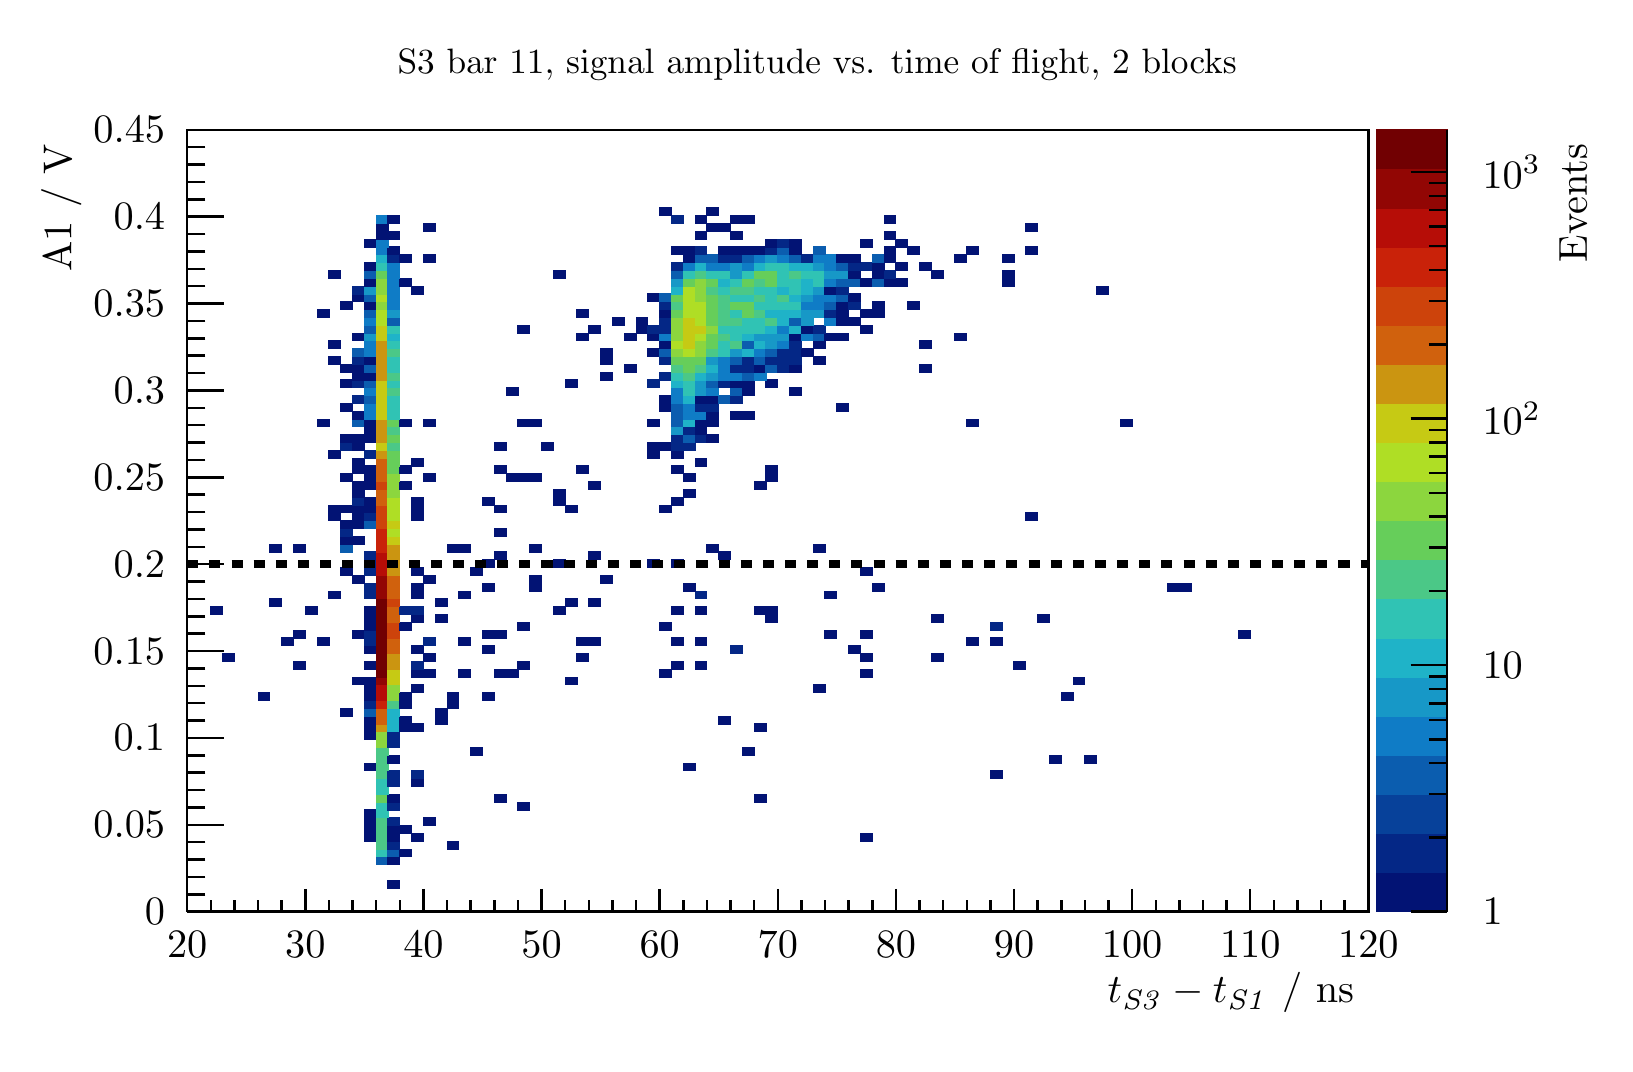
\begin{tikzpicture}
\pgfdeclareplotmark{cross} {
\pgfpathmoveto{\pgfpoint{-0.3\pgfplotmarksize}{\pgfplotmarksize}}
\pgfpathlineto{\pgfpoint{+0.3\pgfplotmarksize}{\pgfplotmarksize}}
\pgfpathlineto{\pgfpoint{+0.3\pgfplotmarksize}{0.3\pgfplotmarksize}}
\pgfpathlineto{\pgfpoint{+1\pgfplotmarksize}{0.3\pgfplotmarksize}}
\pgfpathlineto{\pgfpoint{+1\pgfplotmarksize}{-0.3\pgfplotmarksize}}
\pgfpathlineto{\pgfpoint{+0.3\pgfplotmarksize}{-0.3\pgfplotmarksize}}
\pgfpathlineto{\pgfpoint{+0.3\pgfplotmarksize}{-1.\pgfplotmarksize}}
\pgfpathlineto{\pgfpoint{-0.3\pgfplotmarksize}{-1.\pgfplotmarksize}}
\pgfpathlineto{\pgfpoint{-0.3\pgfplotmarksize}{-0.3\pgfplotmarksize}}
\pgfpathlineto{\pgfpoint{-1.\pgfplotmarksize}{-0.3\pgfplotmarksize}}
\pgfpathlineto{\pgfpoint{-1.\pgfplotmarksize}{0.3\pgfplotmarksize}}
\pgfpathlineto{\pgfpoint{-0.3\pgfplotmarksize}{0.3\pgfplotmarksize}}
\pgfpathclose
\pgfusepathqstroke
}
\pgfdeclareplotmark{cross*} {
\pgfpathmoveto{\pgfpoint{-0.3\pgfplotmarksize}{\pgfplotmarksize}}
\pgfpathlineto{\pgfpoint{+0.3\pgfplotmarksize}{\pgfplotmarksize}}
\pgfpathlineto{\pgfpoint{+0.3\pgfplotmarksize}{0.3\pgfplotmarksize}}
\pgfpathlineto{\pgfpoint{+1\pgfplotmarksize}{0.3\pgfplotmarksize}}
\pgfpathlineto{\pgfpoint{+1\pgfplotmarksize}{-0.3\pgfplotmarksize}}
\pgfpathlineto{\pgfpoint{+0.3\pgfplotmarksize}{-0.3\pgfplotmarksize}}
\pgfpathlineto{\pgfpoint{+0.3\pgfplotmarksize}{-1.\pgfplotmarksize}}
\pgfpathlineto{\pgfpoint{-0.3\pgfplotmarksize}{-1.\pgfplotmarksize}}
\pgfpathlineto{\pgfpoint{-0.3\pgfplotmarksize}{-0.3\pgfplotmarksize}}
\pgfpathlineto{\pgfpoint{-1.\pgfplotmarksize}{-0.3\pgfplotmarksize}}
\pgfpathlineto{\pgfpoint{-1.\pgfplotmarksize}{0.3\pgfplotmarksize}}
\pgfpathlineto{\pgfpoint{-0.3\pgfplotmarksize}{0.3\pgfplotmarksize}}
\pgfpathclose
\pgfusepathqfillstroke
}
\pgfdeclareplotmark{newstar} {
\pgfpathmoveto{\pgfqpoint{0pt}{\pgfplotmarksize}}
\pgfpathlineto{\pgfqpointpolar{44}{0.5\pgfplotmarksize}}
\pgfpathlineto{\pgfqpointpolar{18}{\pgfplotmarksize}}
\pgfpathlineto{\pgfqpointpolar{-20}{0.5\pgfplotmarksize}}
\pgfpathlineto{\pgfqpointpolar{-54}{\pgfplotmarksize}}
\pgfpathlineto{\pgfqpointpolar{-90}{0.5\pgfplotmarksize}}
\pgfpathlineto{\pgfqpointpolar{234}{\pgfplotmarksize}}
\pgfpathlineto{\pgfqpointpolar{198}{0.5\pgfplotmarksize}}
\pgfpathlineto{\pgfqpointpolar{162}{\pgfplotmarksize}}
\pgfpathlineto{\pgfqpointpolar{134}{0.5\pgfplotmarksize}}
\pgfpathclose
\pgfusepathqstroke
}
\pgfdeclareplotmark{newstar*} {
\pgfpathmoveto{\pgfqpoint{0pt}{\pgfplotmarksize}}
\pgfpathlineto{\pgfqpointpolar{44}{0.5\pgfplotmarksize}}
\pgfpathlineto{\pgfqpointpolar{18}{\pgfplotmarksize}}
\pgfpathlineto{\pgfqpointpolar{-20}{0.5\pgfplotmarksize}}
\pgfpathlineto{\pgfqpointpolar{-54}{\pgfplotmarksize}}
\pgfpathlineto{\pgfqpointpolar{-90}{0.5\pgfplotmarksize}}
\pgfpathlineto{\pgfqpointpolar{234}{\pgfplotmarksize}}
\pgfpathlineto{\pgfqpointpolar{198}{0.5\pgfplotmarksize}}
\pgfpathlineto{\pgfqpointpolar{162}{\pgfplotmarksize}}
\pgfpathlineto{\pgfqpointpolar{134}{0.5\pgfplotmarksize}}
\pgfpathclose
\pgfusepathqfillstroke
}
\definecolor{c}{rgb}{1,1,1};
\draw [color=c, fill=c] (0,0) rectangle (20,12.8962);
\draw [color=c, fill=c] (2,1.6765) rectangle (17,11.6066);
\definecolor{c}{rgb}{0,0,0};
\draw [c,line width=0.9] (2,1.6765) -- (2,11.6066) -- (17,11.6066) -- (17,1.6765) -- (2,1.6765);
\definecolor{c}{rgb}{1,1,1};
\draw [color=c, fill=c] (2,1.6765) rectangle (17,11.6066);
\definecolor{c}{rgb}{0,0,0};
\draw [c,line width=0.9] (2,1.6765) -- (2,11.6066) -- (17,11.6066) -- (17,1.6765) -- (2,1.6765);
\definecolor{c}{rgb}{0.00759013,0.0728653,0.45351};
\draw [color=c, fill=c] (4.55,1.9744) rectangle (4.7,2.0737);
\definecolor{c}{rgb}{0.0428922,0.365196,0.687255};
\draw [color=c, fill=c] (4.4,2.27231) rectangle (4.55,2.37161);
\definecolor{c}{rgb}{0.00759013,0.0728653,0.45351};
\draw [color=c, fill=c] (4.55,2.27231) rectangle (4.7,2.37161);
\definecolor{c}{rgb}{0.18652,0.763235,0.706618};
\draw [color=c, fill=c] (4.4,2.37161) rectangle (4.55,2.47091);
\definecolor{c}{rgb}{0.0428922,0.365196,0.687255};
\draw [color=c, fill=c] (4.55,2.37161) rectangle (4.7,2.47091);
\definecolor{c}{rgb}{0.00759013,0.0728653,0.45351};
\draw [color=c, fill=c] (4.7,2.37161) rectangle (4.85,2.47091);
\definecolor{c}{rgb}{0.29326,0.785539,0.529779};
\draw [color=c, fill=c] (4.4,2.47091) rectangle (4.55,2.57021);
\definecolor{c}{rgb}{0.0158128,0.151803,0.524225};
\draw [color=c, fill=c] (4.55,2.47091) rectangle (4.7,2.57021);
\definecolor{c}{rgb}{0.00759013,0.0728653,0.45351};
\draw [color=c, fill=c] (5.3,2.47091) rectangle (5.45,2.57021);
\draw [color=c, fill=c] (4.25,2.57021) rectangle (4.4,2.66951);
\definecolor{c}{rgb}{0.29326,0.785539,0.529779};
\draw [color=c, fill=c] (4.4,2.57021) rectangle (4.55,2.66951);
\definecolor{c}{rgb}{0.00759013,0.0728653,0.45351};
\draw [color=c, fill=c] (4.55,2.57021) rectangle (4.7,2.66951);
\draw [color=c, fill=c] (4.85,2.57021) rectangle (5,2.66951);
\draw [color=c, fill=c] (10.55,2.57021) rectangle (10.7,2.66951);
\draw [color=c, fill=c] (4.25,2.66951) rectangle (4.4,2.76881);
\definecolor{c}{rgb}{0.29326,0.785539,0.529779};
\draw [color=c, fill=c] (4.4,2.66951) rectangle (4.55,2.76881);
\definecolor{c}{rgb}{0.00759013,0.0728653,0.45351};
\draw [color=c, fill=c] (4.55,2.66951) rectangle (4.7,2.76881);
\draw [color=c, fill=c] (4.7,2.66951) rectangle (4.85,2.76881);
\draw [color=c, fill=c] (4.25,2.76881) rectangle (4.4,2.86811);
\definecolor{c}{rgb}{0.29326,0.785539,0.529779};
\draw [color=c, fill=c] (4.4,2.76881) rectangle (4.55,2.86811);
\definecolor{c}{rgb}{0.0158128,0.151803,0.524225};
\draw [color=c, fill=c] (4.55,2.76881) rectangle (4.7,2.86811);
\definecolor{c}{rgb}{0.00759013,0.0728653,0.45351};
\draw [color=c, fill=c] (5,2.76881) rectangle (5.15,2.86811);
\draw [color=c, fill=c] (4.25,2.86811) rectangle (4.4,2.96741);
\definecolor{c}{rgb}{0.18652,0.763235,0.706618};
\draw [color=c, fill=c] (4.4,2.86811) rectangle (4.55,2.96741);
\draw [color=c, fill=c] (4.4,2.96741) rectangle (4.55,3.06671);
\definecolor{c}{rgb}{0.0158128,0.151803,0.524225};
\draw [color=c, fill=c] (4.55,2.96741) rectangle (4.7,3.06671);
\definecolor{c}{rgb}{0.00759013,0.0728653,0.45351};
\draw [color=c, fill=c] (6.2,2.96741) rectangle (6.35,3.06671);
\definecolor{c}{rgb}{0.4,0.807843,0.352941};
\draw [color=c, fill=c] (4.4,3.06671) rectangle (4.55,3.16601);
\definecolor{c}{rgb}{0.00759013,0.0728653,0.45351};
\draw [color=c, fill=c] (4.55,3.06671) rectangle (4.7,3.16601);
\draw [color=c, fill=c] (5.9,3.06671) rectangle (6.05,3.16601);
\draw [color=c, fill=c] (9.2,3.06671) rectangle (9.35,3.16601);
\definecolor{c}{rgb}{0.18652,0.763235,0.706618};
\draw [color=c, fill=c] (4.4,3.16601) rectangle (4.55,3.26531);
\draw [color=c, fill=c] (4.4,3.26531) rectangle (4.55,3.36461);
\definecolor{c}{rgb}{0.0158128,0.151803,0.524225};
\draw [color=c, fill=c] (4.55,3.26531) rectangle (4.7,3.36461);
\definecolor{c}{rgb}{0.00759013,0.0728653,0.45351};
\draw [color=c, fill=c] (4.85,3.26531) rectangle (5,3.36461);
\definecolor{c}{rgb}{0.29326,0.785539,0.529779};
\draw [color=c, fill=c] (4.4,3.36461) rectangle (4.55,3.46391);
\definecolor{c}{rgb}{0.0158128,0.151803,0.524225};
\draw [color=c, fill=c] (4.55,3.36461) rectangle (4.7,3.46391);
\draw [color=c, fill=c] (4.85,3.36461) rectangle (5,3.46391);
\definecolor{c}{rgb}{0.00759013,0.0728653,0.45351};
\draw [color=c, fill=c] (12.2,3.36461) rectangle (12.35,3.46391);
\draw [color=c, fill=c] (4.25,3.46391) rectangle (4.4,3.56321);
\definecolor{c}{rgb}{0.29326,0.785539,0.529779};
\draw [color=c, fill=c] (4.4,3.46391) rectangle (4.55,3.56321);
\definecolor{c}{rgb}{0.00759013,0.0728653,0.45351};
\draw [color=c, fill=c] (8.3,3.46391) rectangle (8.45,3.56321);
\definecolor{c}{rgb}{0.29326,0.785539,0.529779};
\draw [color=c, fill=c] (4.4,3.56321) rectangle (4.55,3.66251);
\definecolor{c}{rgb}{0.00759013,0.0728653,0.45351};
\draw [color=c, fill=c] (4.55,3.56321) rectangle (4.7,3.66251);
\draw [color=c, fill=c] (12.95,3.56321) rectangle (13.1,3.66251);
\draw [color=c, fill=c] (13.4,3.56321) rectangle (13.55,3.66251);
\definecolor{c}{rgb}{0.29326,0.785539,0.529779};
\draw [color=c, fill=c] (4.4,3.66251) rectangle (4.55,3.76181);
\definecolor{c}{rgb}{0.00759013,0.0728653,0.45351};
\draw [color=c, fill=c] (5.6,3.66251) rectangle (5.75,3.76181);
\draw [color=c, fill=c] (9.05,3.66251) rectangle (9.2,3.76181);
\definecolor{c}{rgb}{0.549755,0.839706,0.244608};
\draw [color=c, fill=c] (4.4,3.76181) rectangle (4.55,3.86111);
\definecolor{c}{rgb}{0.0158128,0.151803,0.524225};
\draw [color=c, fill=c] (4.55,3.76181) rectangle (4.7,3.86111);
\definecolor{c}{rgb}{0.00759013,0.0728653,0.45351};
\draw [color=c, fill=c] (4.25,3.86111) rectangle (4.4,3.96042);
\definecolor{c}{rgb}{0.549755,0.839706,0.244608};
\draw [color=c, fill=c] (4.4,3.86111) rectangle (4.55,3.96042);
\definecolor{c}{rgb}{0.0158128,0.151803,0.524225};
\draw [color=c, fill=c] (4.55,3.86111) rectangle (4.7,3.96042);
\definecolor{c}{rgb}{0.00759013,0.0728653,0.45351};
\draw [color=c, fill=c] (4.25,3.96042) rectangle (4.4,4.05972);
\definecolor{c}{rgb}{0.796569,0.585907,0.0653186};
\draw [color=c, fill=c] (4.4,3.96042) rectangle (4.55,4.05972);
\definecolor{c}{rgb}{0.122549,0.702941,0.786029};
\draw [color=c, fill=c] (4.55,3.96042) rectangle (4.7,4.05972);
\definecolor{c}{rgb}{0.00759013,0.0728653,0.45351};
\draw [color=c, fill=c] (4.7,3.96042) rectangle (4.85,4.05972);
\draw [color=c, fill=c] (4.85,3.96042) rectangle (5,4.05972);
\draw [color=c, fill=c] (9.2,3.96042) rectangle (9.35,4.05972);
\draw [color=c, fill=c] (4.25,4.05972) rectangle (4.4,4.15902);
\definecolor{c}{rgb}{0.815686,0.380392,0.0509804};
\draw [color=c, fill=c] (4.4,4.05972) rectangle (4.55,4.15902);
\definecolor{c}{rgb}{0.122549,0.702941,0.786029};
\draw [color=c, fill=c] (4.55,4.05972) rectangle (4.7,4.15902);
\definecolor{c}{rgb}{0.00759013,0.0728653,0.45351};
\draw [color=c, fill=c] (4.7,4.05972) rectangle (4.85,4.15902);
\draw [color=c, fill=c] (5.15,4.05972) rectangle (5.3,4.15902);
\draw [color=c, fill=c] (8.75,4.05972) rectangle (8.9,4.15902);
\draw [color=c, fill=c] (3.95,4.15902) rectangle (4.1,4.25832);
\definecolor{c}{rgb}{0.0428922,0.365196,0.687255};
\draw [color=c, fill=c] (4.25,4.15902) rectangle (4.4,4.25832);
\definecolor{c}{rgb}{0.815686,0.380392,0.0509804};
\draw [color=c, fill=c] (4.4,4.15902) rectangle (4.55,4.25832);
\definecolor{c}{rgb}{0.122549,0.702941,0.786029};
\draw [color=c, fill=c] (4.55,4.15902) rectangle (4.7,4.25832);
\definecolor{c}{rgb}{0.00759013,0.0728653,0.45351};
\draw [color=c, fill=c] (5.15,4.15902) rectangle (5.3,4.25832);
\definecolor{c}{rgb}{0.0158128,0.151803,0.524225};
\draw [color=c, fill=c] (4.25,4.25832) rectangle (4.4,4.35762);
\definecolor{c}{rgb}{0.788113,0.13223,0.0356618};
\draw [color=c, fill=c] (4.4,4.25832) rectangle (4.55,4.35762);
\definecolor{c}{rgb}{0.29326,0.785539,0.529779};
\draw [color=c, fill=c] (4.55,4.25832) rectangle (4.7,4.35762);
\definecolor{c}{rgb}{0.00759013,0.0728653,0.45351};
\draw [color=c, fill=c] (4.7,4.25832) rectangle (4.85,4.35762);
\draw [color=c, fill=c] (5.3,4.25832) rectangle (5.45,4.35762);
\draw [color=c, fill=c] (2.9,4.35762) rectangle (3.05,4.45692);
\draw [color=c, fill=c] (4.25,4.35762) rectangle (4.4,4.45692);
\definecolor{c}{rgb}{0.714951,0.0509804,0.0269608};
\draw [color=c, fill=c] (4.4,4.35762) rectangle (4.55,4.45692);
\definecolor{c}{rgb}{0.549755,0.839706,0.244608};
\draw [color=c, fill=c] (4.55,4.35762) rectangle (4.7,4.45692);
\definecolor{c}{rgb}{0.00759013,0.0728653,0.45351};
\draw [color=c, fill=c] (4.7,4.35762) rectangle (4.85,4.45692);
\draw [color=c, fill=c] (5.3,4.35762) rectangle (5.45,4.45692);
\draw [color=c, fill=c] (5.75,4.35762) rectangle (5.9,4.45692);
\draw [color=c, fill=c] (13.1,4.35762) rectangle (13.25,4.45692);
\draw [color=c, fill=c] (4.25,4.45692) rectangle (4.4,4.55622);
\definecolor{c}{rgb}{0.714951,0.0509804,0.0269608};
\draw [color=c, fill=c] (4.4,4.45692) rectangle (4.55,4.55622);
\definecolor{c}{rgb}{0.549755,0.839706,0.244608};
\draw [color=c, fill=c] (4.55,4.45692) rectangle (4.7,4.55622);
\definecolor{c}{rgb}{0.00759013,0.0728653,0.45351};
\draw [color=c, fill=c] (4.85,4.45692) rectangle (5,4.55622);
\draw [color=c, fill=c] (9.95,4.45692) rectangle (10.1,4.55622);
\draw [color=c, fill=c] (4.1,4.55622) rectangle (4.25,4.65552);
\draw [color=c, fill=c] (4.25,4.55622) rectangle (4.4,4.65552);
\definecolor{c}{rgb}{0.573162,0.0254902,0.017402};
\draw [color=c, fill=c] (4.4,4.55622) rectangle (4.55,4.65552);
\definecolor{c}{rgb}{0.777451,0.791422,0.0796569};
\draw [color=c, fill=c] (4.55,4.55622) rectangle (4.7,4.65552);
\definecolor{c}{rgb}{0.00759013,0.0728653,0.45351};
\draw [color=c, fill=c] (6.8,4.55622) rectangle (6.95,4.65552);
\draw [color=c, fill=c] (13.25,4.55622) rectangle (13.4,4.65552);
\definecolor{c}{rgb}{0.442279,0.00196078,0.00857843};
\draw [color=c, fill=c] (4.4,4.65552) rectangle (4.55,4.75482);
\definecolor{c}{rgb}{0.777451,0.791422,0.0796569};
\draw [color=c, fill=c] (4.55,4.65552) rectangle (4.7,4.75482);
\definecolor{c}{rgb}{0.00759013,0.0728653,0.45351};
\draw [color=c, fill=c] (4.85,4.65552) rectangle (5,4.75482);
\draw [color=c, fill=c] (5,4.65552) rectangle (5.15,4.75482);
\draw [color=c, fill=c] (5.45,4.65552) rectangle (5.6,4.75482);
\draw [color=c, fill=c] (5.9,4.65552) rectangle (6.05,4.75482);
\draw [color=c, fill=c] (6.05,4.65552) rectangle (6.2,4.75482);
\draw [color=c, fill=c] (8,4.65552) rectangle (8.15,4.75482);
\draw [color=c, fill=c] (10.55,4.65552) rectangle (10.7,4.75482);
\draw [color=c, fill=c] (3.35,4.75482) rectangle (3.5,4.85412);
\draw [color=c, fill=c] (4.25,4.75482) rectangle (4.4,4.85412);
\definecolor{c}{rgb}{0.442279,0.00196078,0.00857843};
\draw [color=c, fill=c] (4.4,4.75482) rectangle (4.55,4.85412);
\definecolor{c}{rgb}{0.796569,0.585907,0.0653186};
\draw [color=c, fill=c] (4.55,4.75482) rectangle (4.7,4.85412);
\definecolor{c}{rgb}{0.0158128,0.151803,0.524225};
\draw [color=c, fill=c] (4.85,4.75482) rectangle (5,4.85412);
\definecolor{c}{rgb}{0.00759013,0.0728653,0.45351};
\draw [color=c, fill=c] (6.2,4.75482) rectangle (6.35,4.85412);
\draw [color=c, fill=c] (8.15,4.75482) rectangle (8.3,4.85412);
\draw [color=c, fill=c] (8.45,4.75482) rectangle (8.6,4.85412);
\draw [color=c, fill=c] (12.5,4.75482) rectangle (12.65,4.85412);
\draw [color=c, fill=c] (2.45,4.85412) rectangle (2.6,4.95342);
\definecolor{c}{rgb}{0.442279,0.00196078,0.00857843};
\draw [color=c, fill=c] (4.4,4.85412) rectangle (4.55,4.95342);
\definecolor{c}{rgb}{0.796569,0.585907,0.0653186};
\draw [color=c, fill=c] (4.55,4.85412) rectangle (4.7,4.95342);
\definecolor{c}{rgb}{0.00759013,0.0728653,0.45351};
\draw [color=c, fill=c] (5,4.85412) rectangle (5.15,4.95342);
\draw [color=c, fill=c] (6.95,4.85412) rectangle (7.1,4.95342);
\draw [color=c, fill=c] (10.55,4.85412) rectangle (10.7,4.95342);
\draw [color=c, fill=c] (11.45,4.85412) rectangle (11.6,4.95342);
\draw [color=c, fill=c] (4.25,4.95342) rectangle (4.4,5.05272);
\definecolor{c}{rgb}{0.442279,0.00196078,0.00857843};
\draw [color=c, fill=c] (4.4,4.95342) rectangle (4.55,5.05272);
\definecolor{c}{rgb}{0.815686,0.380392,0.0509804};
\draw [color=c, fill=c] (4.55,4.95342) rectangle (4.7,5.05272);
\definecolor{c}{rgb}{0.00759013,0.0728653,0.45351};
\draw [color=c, fill=c] (4.85,4.95342) rectangle (5,5.05272);
\draw [color=c, fill=c] (5.75,4.95342) rectangle (5.9,5.05272);
\definecolor{c}{rgb}{0.0158128,0.151803,0.524225};
\draw [color=c, fill=c] (8.9,4.95342) rectangle (9.05,5.05272);
\definecolor{c}{rgb}{0.00759013,0.0728653,0.45351};
\draw [color=c, fill=c] (10.4,4.95342) rectangle (10.55,5.05272);
\draw [color=c, fill=c] (3.2,5.05272) rectangle (3.35,5.15202);
\draw [color=c, fill=c] (3.65,5.05272) rectangle (3.8,5.15202);
\definecolor{c}{rgb}{0.0158128,0.151803,0.524225};
\draw [color=c, fill=c] (4.25,5.05272) rectangle (4.4,5.15202);
\definecolor{c}{rgb}{0.442279,0.00196078,0.00857843};
\draw [color=c, fill=c] (4.4,5.05272) rectangle (4.55,5.15202);
\definecolor{c}{rgb}{0.815686,0.380392,0.0509804};
\draw [color=c, fill=c] (4.55,5.05272) rectangle (4.7,5.15202);
\definecolor{c}{rgb}{0.0158128,0.151803,0.524225};
\draw [color=c, fill=c] (5,5.05272) rectangle (5.15,5.15202);
\definecolor{c}{rgb}{0.00759013,0.0728653,0.45351};
\draw [color=c, fill=c] (5.45,5.05272) rectangle (5.6,5.15202);
\draw [color=c, fill=c] (6.95,5.05272) rectangle (7.1,5.15202);
\draw [color=c, fill=c] (7.1,5.05272) rectangle (7.25,5.15202);
\draw [color=c, fill=c] (8.15,5.05272) rectangle (8.3,5.15202);
\draw [color=c, fill=c] (8.45,5.05272) rectangle (8.6,5.15202);
\draw [color=c, fill=c] (11.9,5.05272) rectangle (12.05,5.15202);
\draw [color=c, fill=c] (12.2,5.05272) rectangle (12.35,5.15202);
\draw [color=c, fill=c] (3.35,5.15202) rectangle (3.5,5.25132);
\draw [color=c, fill=c] (4.1,5.15202) rectangle (4.25,5.25132);
\definecolor{c}{rgb}{0.0158128,0.151803,0.524225};
\draw [color=c, fill=c] (4.25,5.15202) rectangle (4.4,5.25132);
\definecolor{c}{rgb}{0.442279,0.00196078,0.00857843};
\draw [color=c, fill=c] (4.4,5.15202) rectangle (4.55,5.25132);
\definecolor{c}{rgb}{0.802451,0.261275,0.0436275};
\draw [color=c, fill=c] (4.55,5.15202) rectangle (4.7,5.25132);
\definecolor{c}{rgb}{0.00759013,0.0728653,0.45351};
\draw [color=c, fill=c] (5.75,5.15202) rectangle (5.9,5.25132);
\draw [color=c, fill=c] (5.9,5.15202) rectangle (6.05,5.25132);
\draw [color=c, fill=c] (10.1,5.15202) rectangle (10.25,5.25132);
\draw [color=c, fill=c] (10.55,5.15202) rectangle (10.7,5.25132);
\draw [color=c, fill=c] (15.35,5.15202) rectangle (15.5,5.25132);
\draw [color=c, fill=c] (4.25,5.25132) rectangle (4.4,5.35062);
\definecolor{c}{rgb}{0.442279,0.00196078,0.00857843};
\draw [color=c, fill=c] (4.4,5.25132) rectangle (4.55,5.35062);
\definecolor{c}{rgb}{0.802451,0.261275,0.0436275};
\draw [color=c, fill=c] (4.55,5.25132) rectangle (4.7,5.35062);
\definecolor{c}{rgb}{0.00759013,0.0728653,0.45351};
\draw [color=c, fill=c] (4.7,5.25132) rectangle (4.85,5.35062);
\draw [color=c, fill=c] (6.2,5.25132) rectangle (6.35,5.35062);
\draw [color=c, fill=c] (8,5.25132) rectangle (8.15,5.35062);
\definecolor{c}{rgb}{0.0158128,0.151803,0.524225};
\draw [color=c, fill=c] (12.2,5.25132) rectangle (12.35,5.35062);
\definecolor{c}{rgb}{0.00759013,0.0728653,0.45351};
\draw [color=c, fill=c] (4.25,5.35062) rectangle (4.4,5.44992);
\definecolor{c}{rgb}{0.442279,0.00196078,0.00857843};
\draw [color=c, fill=c] (4.4,5.35062) rectangle (4.55,5.44992);
\definecolor{c}{rgb}{0.815686,0.380392,0.0509804};
\draw [color=c, fill=c] (4.55,5.35062) rectangle (4.7,5.44992);
\definecolor{c}{rgb}{0.00759013,0.0728653,0.45351};
\draw [color=c, fill=c] (4.85,5.35062) rectangle (5,5.44992);
\draw [color=c, fill=c] (5.15,5.35062) rectangle (5.3,5.44992);
\draw [color=c, fill=c] (9.35,5.35062) rectangle (9.5,5.44992);
\draw [color=c, fill=c] (11.45,5.35062) rectangle (11.6,5.44992);
\draw [color=c, fill=c] (12.8,5.35062) rectangle (12.95,5.44992);
\draw [color=c, fill=c] (2.3,5.44992) rectangle (2.45,5.54922);
\draw [color=c, fill=c] (3.5,5.44992) rectangle (3.65,5.54922);
\draw [color=c, fill=c] (4.25,5.44992) rectangle (4.4,5.54922);
\definecolor{c}{rgb}{0.442279,0.00196078,0.00857843};
\draw [color=c, fill=c] (4.4,5.44992) rectangle (4.55,5.54922);
\definecolor{c}{rgb}{0.815686,0.380392,0.0509804};
\draw [color=c, fill=c] (4.55,5.44992) rectangle (4.7,5.54922);
\definecolor{c}{rgb}{0.0158128,0.151803,0.524225};
\draw [color=c, fill=c] (4.7,5.44992) rectangle (4.85,5.54922);
\draw [color=c, fill=c] (4.85,5.44992) rectangle (5,5.54922);
\definecolor{c}{rgb}{0.00759013,0.0728653,0.45351};
\draw [color=c, fill=c] (6.65,5.44992) rectangle (6.8,5.54922);
\draw [color=c, fill=c] (8.15,5.44992) rectangle (8.3,5.54922);
\draw [color=c, fill=c] (8.45,5.44992) rectangle (8.6,5.54922);
\draw [color=c, fill=c] (9.2,5.44992) rectangle (9.35,5.54922);
\draw [color=c, fill=c] (9.35,5.44992) rectangle (9.5,5.54922);
\draw [color=c, fill=c] (3.05,5.54922) rectangle (3.2,5.64852);
\definecolor{c}{rgb}{0.442279,0.00196078,0.00857843};
\draw [color=c, fill=c] (4.4,5.54922) rectangle (4.55,5.64852);
\definecolor{c}{rgb}{0.802451,0.261275,0.0436275};
\draw [color=c, fill=c] (4.55,5.54922) rectangle (4.7,5.64852);
\definecolor{c}{rgb}{0.00759013,0.0728653,0.45351};
\draw [color=c, fill=c] (5.15,5.54922) rectangle (5.3,5.64852);
\draw [color=c, fill=c] (6.8,5.54922) rectangle (6.95,5.64852);
\draw [color=c, fill=c] (7.1,5.54922) rectangle (7.25,5.64852);
\draw [color=c, fill=c] (3.8,5.64852) rectangle (3.95,5.74783);
\definecolor{c}{rgb}{0.0158128,0.151803,0.524225};
\draw [color=c, fill=c] (4.25,5.64852) rectangle (4.4,5.74783);
\definecolor{c}{rgb}{0.573162,0.0254902,0.017402};
\draw [color=c, fill=c] (4.4,5.64852) rectangle (4.55,5.74783);
\definecolor{c}{rgb}{0.815686,0.380392,0.0509804};
\draw [color=c, fill=c] (4.55,5.64852) rectangle (4.7,5.74783);
\definecolor{c}{rgb}{0.00759013,0.0728653,0.45351};
\draw [color=c, fill=c] (4.85,5.64852) rectangle (5,5.74783);
\draw [color=c, fill=c] (5.45,5.64852) rectangle (5.6,5.74783);
\definecolor{c}{rgb}{0.0158128,0.151803,0.524225};
\draw [color=c, fill=c] (8.45,5.64852) rectangle (8.6,5.74783);
\definecolor{c}{rgb}{0.00759013,0.0728653,0.45351};
\draw [color=c, fill=c] (10.1,5.64852) rectangle (10.25,5.74783);
\definecolor{c}{rgb}{0.0158128,0.151803,0.524225};
\draw [color=c, fill=c] (4.25,5.74783) rectangle (4.4,5.84713);
\definecolor{c}{rgb}{0.573162,0.0254902,0.017402};
\draw [color=c, fill=c] (4.4,5.74783) rectangle (4.55,5.84713);
\definecolor{c}{rgb}{0.815686,0.380392,0.0509804};
\draw [color=c, fill=c] (4.55,5.74783) rectangle (4.7,5.84713);
\definecolor{c}{rgb}{0.00759013,0.0728653,0.45351};
\draw [color=c, fill=c] (4.85,5.74783) rectangle (5,5.84713);
\draw [color=c, fill=c] (5.75,5.74783) rectangle (5.9,5.84713);
\draw [color=c, fill=c] (6.35,5.74783) rectangle (6.5,5.84713);
\draw [color=c, fill=c] (8.3,5.74783) rectangle (8.45,5.84713);
\draw [color=c, fill=c] (10.7,5.74783) rectangle (10.85,5.84713);
\draw [color=c, fill=c] (14.45,5.74783) rectangle (14.6,5.84713);
\draw [color=c, fill=c] (14.6,5.74783) rectangle (14.75,5.84713);
\draw [color=c, fill=c] (4.1,5.84713) rectangle (4.25,5.94643);
\definecolor{c}{rgb}{0.573162,0.0254902,0.017402};
\draw [color=c, fill=c] (4.4,5.84713) rectangle (4.55,5.94643);
\definecolor{c}{rgb}{0.815686,0.380392,0.0509804};
\draw [color=c, fill=c] (4.55,5.84713) rectangle (4.7,5.94643);
\definecolor{c}{rgb}{0.00759013,0.0728653,0.45351};
\draw [color=c, fill=c] (5,5.84713) rectangle (5.15,5.94643);
\draw [color=c, fill=c] (6.35,5.84713) rectangle (6.5,5.94643);
\draw [color=c, fill=c] (7.25,5.84713) rectangle (7.4,5.94643);
\draw [color=c, fill=c] (3.95,5.94643) rectangle (4.1,6.04573);
\definecolor{c}{rgb}{0.0158128,0.151803,0.524225};
\draw [color=c, fill=c] (4.25,5.94643) rectangle (4.4,6.04573);
\definecolor{c}{rgb}{0.714951,0.0509804,0.0269608};
\draw [color=c, fill=c] (4.4,5.94643) rectangle (4.55,6.04573);
\definecolor{c}{rgb}{0.796569,0.585907,0.0653186};
\draw [color=c, fill=c] (4.55,5.94643) rectangle (4.7,6.04573);
\definecolor{c}{rgb}{0.00759013,0.0728653,0.45351};
\draw [color=c, fill=c] (4.85,5.94643) rectangle (5,6.04573);
\draw [color=c, fill=c] (5.6,5.94643) rectangle (5.75,6.04573);
\draw [color=c, fill=c] (10.55,5.94643) rectangle (10.7,6.04573);
\definecolor{c}{rgb}{0.0158128,0.151803,0.524225};
\draw [color=c, fill=c] (4.25,6.04573) rectangle (4.4,6.14503);
\definecolor{c}{rgb}{0.714951,0.0509804,0.0269608};
\draw [color=c, fill=c] (4.4,6.04573) rectangle (4.55,6.14503);
\definecolor{c}{rgb}{0.796569,0.585907,0.0653186};
\draw [color=c, fill=c] (4.55,6.04573) rectangle (4.7,6.14503);
\definecolor{c}{rgb}{0.00759013,0.0728653,0.45351};
\draw [color=c, fill=c] (5.75,6.04573) rectangle (5.9,6.14503);
\draw [color=c, fill=c] (6.65,6.04573) rectangle (6.8,6.14503);
\draw [color=c, fill=c] (7.85,6.04573) rectangle (8,6.14503);
\draw [color=c, fill=c] (8.15,6.04573) rectangle (8.3,6.14503);
\definecolor{c}{rgb}{0.0158128,0.151803,0.524225};
\draw [color=c, fill=c] (4.25,6.14503) rectangle (4.4,6.24433);
\definecolor{c}{rgb}{0.714951,0.0509804,0.0269608};
\draw [color=c, fill=c] (4.4,6.14503) rectangle (4.55,6.24433);
\definecolor{c}{rgb}{0.796569,0.585907,0.0653186};
\draw [color=c, fill=c] (4.55,6.14503) rectangle (4.7,6.24433);
\definecolor{c}{rgb}{0.00759013,0.0728653,0.45351};
\draw [color=c, fill=c] (5.9,6.14503) rectangle (6.05,6.24433);
\draw [color=c, fill=c] (7.1,6.14503) rectangle (7.25,6.24433);
\draw [color=c, fill=c] (8.75,6.14503) rectangle (8.9,6.24433);
\draw [color=c, fill=c] (3.05,6.24433) rectangle (3.2,6.34363);
\draw [color=c, fill=c] (3.35,6.24433) rectangle (3.5,6.34363);
\definecolor{c}{rgb}{0.0428922,0.365196,0.687255};
\draw [color=c, fill=c] (3.95,6.24433) rectangle (4.1,6.34363);
\definecolor{c}{rgb}{0.788113,0.13223,0.0356618};
\draw [color=c, fill=c] (4.4,6.24433) rectangle (4.55,6.34363);
\definecolor{c}{rgb}{0.796569,0.585907,0.0653186};
\draw [color=c, fill=c] (4.55,6.24433) rectangle (4.7,6.34363);
\definecolor{c}{rgb}{0.00759013,0.0728653,0.45351};
\draw [color=c, fill=c] (5.3,6.24433) rectangle (5.45,6.34363);
\draw [color=c, fill=c] (5.45,6.24433) rectangle (5.6,6.34363);
\draw [color=c, fill=c] (6.35,6.24433) rectangle (6.5,6.34363);
\draw [color=c, fill=c] (8.6,6.24433) rectangle (8.75,6.34363);
\draw [color=c, fill=c] (9.95,6.24433) rectangle (10.1,6.34363);
\draw [color=c, fill=c] (3.95,6.34363) rectangle (4.1,6.44293);
\draw [color=c, fill=c] (4.1,6.34363) rectangle (4.25,6.44293);
\definecolor{c}{rgb}{0.788113,0.13223,0.0356618};
\draw [color=c, fill=c] (4.4,6.34363) rectangle (4.55,6.44293);
\definecolor{c}{rgb}{0.777451,0.791422,0.0796569};
\draw [color=c, fill=c] (4.55,6.34363) rectangle (4.7,6.44293);
\definecolor{c}{rgb}{0.0158128,0.151803,0.524225};
\draw [color=c, fill=c] (3.95,6.44293) rectangle (4.1,6.54223);
\definecolor{c}{rgb}{0.788113,0.13223,0.0356618};
\draw [color=c, fill=c] (4.4,6.44293) rectangle (4.55,6.54223);
\definecolor{c}{rgb}{0.68799,0.869118,0.144608};
\draw [color=c, fill=c] (4.55,6.44293) rectangle (4.7,6.54223);
\definecolor{c}{rgb}{0.00759013,0.0728653,0.45351};
\draw [color=c, fill=c] (5.9,6.44293) rectangle (6.05,6.54223);
\draw [color=c, fill=c] (3.95,6.54223) rectangle (4.1,6.64153);
\draw [color=c, fill=c] (4.1,6.54223) rectangle (4.25,6.64153);
\definecolor{c}{rgb}{0.0428922,0.365196,0.687255};
\draw [color=c, fill=c] (4.25,6.54223) rectangle (4.4,6.64153);
\definecolor{c}{rgb}{0.802451,0.261275,0.0436275};
\draw [color=c, fill=c] (4.4,6.54223) rectangle (4.55,6.64153);
\definecolor{c}{rgb}{0.777451,0.791422,0.0796569};
\draw [color=c, fill=c] (4.55,6.54223) rectangle (4.7,6.64153);
\definecolor{c}{rgb}{0.00759013,0.0728653,0.45351};
\draw [color=c, fill=c] (3.8,6.64153) rectangle (3.95,6.74083);
\draw [color=c, fill=c] (4.1,6.64153) rectangle (4.25,6.74083);
\definecolor{c}{rgb}{0.0158128,0.151803,0.524225};
\draw [color=c, fill=c] (4.25,6.64153) rectangle (4.4,6.74083);
\definecolor{c}{rgb}{0.802451,0.261275,0.0436275};
\draw [color=c, fill=c] (4.4,6.64153) rectangle (4.55,6.74083);
\definecolor{c}{rgb}{0.68799,0.869118,0.144608};
\draw [color=c, fill=c] (4.55,6.64153) rectangle (4.7,6.74083);
\definecolor{c}{rgb}{0.00759013,0.0728653,0.45351};
\draw [color=c, fill=c] (4.85,6.64153) rectangle (5,6.74083);
\draw [color=c, fill=c] (12.65,6.64153) rectangle (12.8,6.74083);
\draw [color=c, fill=c] (3.8,6.74083) rectangle (3.95,6.84013);
\draw [color=c, fill=c] (3.95,6.74083) rectangle (4.1,6.84013);
\draw [color=c, fill=c] (4.1,6.74083) rectangle (4.25,6.84013);
\draw [color=c, fill=c] (4.25,6.74083) rectangle (4.4,6.84013);
\definecolor{c}{rgb}{0.802451,0.261275,0.0436275};
\draw [color=c, fill=c] (4.4,6.74083) rectangle (4.55,6.84013);
\definecolor{c}{rgb}{0.68799,0.869118,0.144608};
\draw [color=c, fill=c] (4.55,6.74083) rectangle (4.7,6.84013);
\definecolor{c}{rgb}{0.00759013,0.0728653,0.45351};
\draw [color=c, fill=c] (4.85,6.74083) rectangle (5,6.84013);
\draw [color=c, fill=c] (5.9,6.74083) rectangle (6.05,6.84013);
\draw [color=c, fill=c] (6.8,6.74083) rectangle (6.95,6.84013);
\draw [color=c, fill=c] (8,6.74083) rectangle (8.15,6.84013);
\definecolor{c}{rgb}{0.0158128,0.151803,0.524225};
\draw [color=c, fill=c] (4.1,6.84013) rectangle (4.25,6.93943);
\definecolor{c}{rgb}{0.00759013,0.0728653,0.45351};
\draw [color=c, fill=c] (4.25,6.84013) rectangle (4.4,6.93943);
\definecolor{c}{rgb}{0.815686,0.380392,0.0509804};
\draw [color=c, fill=c] (4.4,6.84013) rectangle (4.55,6.93943);
\definecolor{c}{rgb}{0.68799,0.869118,0.144608};
\draw [color=c, fill=c] (4.55,6.84013) rectangle (4.7,6.93943);
\definecolor{c}{rgb}{0.00759013,0.0728653,0.45351};
\draw [color=c, fill=c] (4.85,6.84013) rectangle (5,6.93943);
\draw [color=c, fill=c] (5.75,6.84013) rectangle (5.9,6.93943);
\draw [color=c, fill=c] (6.65,6.84013) rectangle (6.8,6.93943);
\draw [color=c, fill=c] (8.15,6.84013) rectangle (8.3,6.93943);
\draw [color=c, fill=c] (4.1,6.93943) rectangle (4.25,7.03873);
\definecolor{c}{rgb}{0.815686,0.380392,0.0509804};
\draw [color=c, fill=c] (4.4,6.93943) rectangle (4.55,7.03873);
\definecolor{c}{rgb}{0.549755,0.839706,0.244608};
\draw [color=c, fill=c] (4.55,6.93943) rectangle (4.7,7.03873);
\definecolor{c}{rgb}{0.00759013,0.0728653,0.45351};
\draw [color=c, fill=c] (6.65,6.93943) rectangle (6.8,7.03873);
\draw [color=c, fill=c] (8.3,6.93943) rectangle (8.45,7.03873);
\draw [color=c, fill=c] (4.1,7.03873) rectangle (4.25,7.13803);
\draw [color=c, fill=c] (4.25,7.03873) rectangle (4.4,7.13803);
\definecolor{c}{rgb}{0.802451,0.261275,0.0436275};
\draw [color=c, fill=c] (4.4,7.03873) rectangle (4.55,7.13803);
\definecolor{c}{rgb}{0.549755,0.839706,0.244608};
\draw [color=c, fill=c] (4.55,7.03873) rectangle (4.7,7.13803);
\definecolor{c}{rgb}{0.00759013,0.0728653,0.45351};
\draw [color=c, fill=c] (4.7,7.03873) rectangle (4.85,7.13803);
\draw [color=c, fill=c] (7.1,7.03873) rectangle (7.25,7.13803);
\draw [color=c, fill=c] (9.2,7.03873) rectangle (9.35,7.13803);
\draw [color=c, fill=c] (3.95,7.13803) rectangle (4.1,7.23733);
\draw [color=c, fill=c] (4.25,7.13803) rectangle (4.4,7.23733);
\definecolor{c}{rgb}{0.815686,0.380392,0.0509804};
\draw [color=c, fill=c] (4.4,7.13803) rectangle (4.55,7.23733);
\definecolor{c}{rgb}{0.549755,0.839706,0.244608};
\draw [color=c, fill=c] (4.55,7.13803) rectangle (4.7,7.23733);
\definecolor{c}{rgb}{0.00759013,0.0728653,0.45351};
\draw [color=c, fill=c] (5,7.13803) rectangle (5.15,7.23733);
\draw [color=c, fill=c] (6.05,7.13803) rectangle (6.2,7.23733);
\draw [color=c, fill=c] (6.2,7.13803) rectangle (6.35,7.23733);
\draw [color=c, fill=c] (6.35,7.13803) rectangle (6.5,7.23733);
\draw [color=c, fill=c] (8.3,7.13803) rectangle (8.45,7.23733);
\draw [color=c, fill=c] (9.35,7.13803) rectangle (9.5,7.23733);
\draw [color=c, fill=c] (4.1,7.23733) rectangle (4.25,7.33663);
\draw [color=c, fill=c] (4.25,7.23733) rectangle (4.4,7.33663);
\definecolor{c}{rgb}{0.815686,0.380392,0.0509804};
\draw [color=c, fill=c] (4.4,7.23733) rectangle (4.55,7.33663);
\definecolor{c}{rgb}{0.4,0.807843,0.352941};
\draw [color=c, fill=c] (4.55,7.23733) rectangle (4.7,7.33663);
\definecolor{c}{rgb}{0.00759013,0.0728653,0.45351};
\draw [color=c, fill=c] (4.7,7.23733) rectangle (4.85,7.33663);
\draw [color=c, fill=c] (5.9,7.23733) rectangle (6.05,7.33663);
\draw [color=c, fill=c] (6.95,7.23733) rectangle (7.1,7.33663);
\draw [color=c, fill=c] (8.15,7.23733) rectangle (8.3,7.33663);
\draw [color=c, fill=c] (9.35,7.23733) rectangle (9.5,7.33663);
\draw [color=c, fill=c] (4.1,7.33663) rectangle (4.25,7.43593);
\definecolor{c}{rgb}{0.815686,0.380392,0.0509804};
\draw [color=c, fill=c] (4.4,7.33663) rectangle (4.55,7.43593);
\definecolor{c}{rgb}{0.4,0.807843,0.352941};
\draw [color=c, fill=c] (4.55,7.33663) rectangle (4.7,7.43593);
\definecolor{c}{rgb}{0.00759013,0.0728653,0.45351};
\draw [color=c, fill=c] (4.85,7.33663) rectangle (5,7.43593);
\draw [color=c, fill=c] (8.45,7.33663) rectangle (8.6,7.43593);
\draw [color=c, fill=c] (3.8,7.43593) rectangle (3.95,7.53523);
\definecolor{c}{rgb}{0.0158128,0.151803,0.524225};
\draw [color=c, fill=c] (4.25,7.43593) rectangle (4.4,7.53523);
\definecolor{c}{rgb}{0.796569,0.585907,0.0653186};
\draw [color=c, fill=c] (4.4,7.43593) rectangle (4.55,7.53523);
\definecolor{c}{rgb}{0.4,0.807843,0.352941};
\draw [color=c, fill=c] (4.55,7.43593) rectangle (4.7,7.53523);
\definecolor{c}{rgb}{0.00759013,0.0728653,0.45351};
\draw [color=c, fill=c] (7.85,7.43593) rectangle (8,7.53523);
\draw [color=c, fill=c] (8.15,7.43593) rectangle (8.3,7.53523);
\definecolor{c}{rgb}{0.0158128,0.151803,0.524225};
\draw [color=c, fill=c] (3.95,7.53523) rectangle (4.1,7.63454);
\definecolor{c}{rgb}{0.00759013,0.0728653,0.45351};
\draw [color=c, fill=c] (4.1,7.53523) rectangle (4.25,7.63454);
\definecolor{c}{rgb}{0.777451,0.791422,0.0796569};
\draw [color=c, fill=c] (4.4,7.53523) rectangle (4.55,7.63454);
\definecolor{c}{rgb}{0.29326,0.785539,0.529779};
\draw [color=c, fill=c] (4.55,7.53523) rectangle (4.7,7.63454);
\definecolor{c}{rgb}{0.00759013,0.0728653,0.45351};
\draw [color=c, fill=c] (5.9,7.53523) rectangle (6.05,7.63454);
\draw [color=c, fill=c] (6.5,7.53523) rectangle (6.65,7.63454);
\draw [color=c, fill=c] (7.85,7.53523) rectangle (8,7.63454);
\draw [color=c, fill=c] (8,7.53523) rectangle (8.15,7.63454);
\definecolor{c}{rgb}{0.0158128,0.151803,0.524225};
\draw [color=c, fill=c] (8.15,7.53523) rectangle (8.3,7.63454);
\draw [color=c, fill=c] (8.3,7.53523) rectangle (8.45,7.63454);
\definecolor{c}{rgb}{0.00759013,0.0728653,0.45351};
\draw [color=c, fill=c] (3.95,7.63454) rectangle (4.1,7.73384);
\draw [color=c, fill=c] (4.1,7.63454) rectangle (4.25,7.73384);
\draw [color=c, fill=c] (4.25,7.63454) rectangle (4.4,7.73384);
\definecolor{c}{rgb}{0.796569,0.585907,0.0653186};
\draw [color=c, fill=c] (4.4,7.63454) rectangle (4.55,7.73384);
\definecolor{c}{rgb}{0.4,0.807843,0.352941};
\draw [color=c, fill=c] (4.55,7.63454) rectangle (4.7,7.73384);
\definecolor{c}{rgb}{0.0158128,0.151803,0.524225};
\draw [color=c, fill=c] (8.15,7.63454) rectangle (8.3,7.73384);
\definecolor{c}{rgb}{0.0428922,0.365196,0.687255};
\draw [color=c, fill=c] (8.3,7.63454) rectangle (8.45,7.73384);
\definecolor{c}{rgb}{0.0158128,0.151803,0.524225};
\draw [color=c, fill=c] (8.45,7.63454) rectangle (8.6,7.73384);
\definecolor{c}{rgb}{0.00759013,0.0728653,0.45351};
\draw [color=c, fill=c] (8.6,7.63454) rectangle (8.75,7.73384);
\draw [color=c, fill=c] (4.25,7.73384) rectangle (4.4,7.83314);
\definecolor{c}{rgb}{0.796569,0.585907,0.0653186};
\draw [color=c, fill=c] (4.4,7.73384) rectangle (4.55,7.83314);
\definecolor{c}{rgb}{0.29326,0.785539,0.529779};
\draw [color=c, fill=c] (4.55,7.73384) rectangle (4.7,7.83314);
\definecolor{c}{rgb}{0.0906863,0.594608,0.78125};
\draw [color=c, fill=c] (8.15,7.73384) rectangle (8.3,7.83314);
\definecolor{c}{rgb}{0.0158128,0.151803,0.524225};
\draw [color=c, fill=c] (8.3,7.73384) rectangle (8.45,7.83314);
\definecolor{c}{rgb}{0.00759013,0.0728653,0.45351};
\draw [color=c, fill=c] (8.45,7.73384) rectangle (8.6,7.83314);
\draw [color=c, fill=c] (3.65,7.83314) rectangle (3.8,7.93244);
\definecolor{c}{rgb}{0.0428922,0.365196,0.687255};
\draw [color=c, fill=c] (4.1,7.83314) rectangle (4.25,7.93244);
\definecolor{c}{rgb}{0.00759013,0.0728653,0.45351};
\draw [color=c, fill=c] (4.25,7.83314) rectangle (4.4,7.93244);
\definecolor{c}{rgb}{0.796569,0.585907,0.0653186};
\draw [color=c, fill=c] (4.4,7.83314) rectangle (4.55,7.93244);
\definecolor{c}{rgb}{0.4,0.807843,0.352941};
\draw [color=c, fill=c] (4.55,7.83314) rectangle (4.7,7.93244);
\definecolor{c}{rgb}{0.00759013,0.0728653,0.45351};
\draw [color=c, fill=c] (4.7,7.83314) rectangle (4.85,7.93244);
\draw [color=c, fill=c] (5,7.83314) rectangle (5.15,7.93244);
\draw [color=c, fill=c] (6.2,7.83314) rectangle (6.35,7.93244);
\draw [color=c, fill=c] (6.35,7.83314) rectangle (6.5,7.93244);
\draw [color=c, fill=c] (7.85,7.83314) rectangle (8,7.93244);
\definecolor{c}{rgb}{0.0428922,0.365196,0.687255};
\draw [color=c, fill=c] (8.15,7.83314) rectangle (8.3,7.93244);
\definecolor{c}{rgb}{0.122549,0.702941,0.786029};
\draw [color=c, fill=c] (8.3,7.83314) rectangle (8.45,7.93244);
\definecolor{c}{rgb}{0.00759013,0.0728653,0.45351};
\draw [color=c, fill=c] (8.45,7.83314) rectangle (8.6,7.93244);
\draw [color=c, fill=c] (8.6,7.83314) rectangle (8.75,7.93244);
\draw [color=c, fill=c] (11.9,7.83314) rectangle (12.05,7.93244);
\draw [color=c, fill=c] (13.85,7.83314) rectangle (14,7.93244);
\draw [color=c, fill=c] (4.1,7.93244) rectangle (4.25,8.03174);
\definecolor{c}{rgb}{0.0588235,0.486275,0.776471};
\draw [color=c, fill=c] (4.25,7.93244) rectangle (4.4,8.03174);
\definecolor{c}{rgb}{0.777451,0.791422,0.0796569};
\draw [color=c, fill=c] (4.4,7.93244) rectangle (4.55,8.03174);
\definecolor{c}{rgb}{0.18652,0.763235,0.706618};
\draw [color=c, fill=c] (4.55,7.93244) rectangle (4.7,8.03174);
\definecolor{c}{rgb}{0.0428922,0.365196,0.687255};
\draw [color=c, fill=c] (8.15,7.93244) rectangle (8.3,8.03174);
\definecolor{c}{rgb}{0.0588235,0.486275,0.776471};
\draw [color=c, fill=c] (8.3,7.93244) rectangle (8.45,8.03174);
\draw [color=c, fill=c] (8.45,7.93244) rectangle (8.6,8.03174);
\definecolor{c}{rgb}{0.00759013,0.0728653,0.45351};
\draw [color=c, fill=c] (8.6,7.93244) rectangle (8.75,8.03174);
\draw [color=c, fill=c] (8.9,7.93244) rectangle (9.05,8.03174);
\draw [color=c, fill=c] (9.05,7.93244) rectangle (9.2,8.03174);
\draw [color=c, fill=c] (3.95,8.03174) rectangle (4.1,8.13104);
\definecolor{c}{rgb}{0.0588235,0.486275,0.776471};
\draw [color=c, fill=c] (4.25,8.03174) rectangle (4.4,8.13104);
\definecolor{c}{rgb}{0.777451,0.791422,0.0796569};
\draw [color=c, fill=c] (4.4,8.03174) rectangle (4.55,8.13104);
\definecolor{c}{rgb}{0.18652,0.763235,0.706618};
\draw [color=c, fill=c] (4.55,8.03174) rectangle (4.7,8.13104);
\definecolor{c}{rgb}{0.00759013,0.0728653,0.45351};
\draw [color=c, fill=c] (8,8.03174) rectangle (8.15,8.13104);
\definecolor{c}{rgb}{0.0428922,0.365196,0.687255};
\draw [color=c, fill=c] (8.15,8.03174) rectangle (8.3,8.13104);
\definecolor{c}{rgb}{0.0588235,0.486275,0.776471};
\draw [color=c, fill=c] (8.3,8.03174) rectangle (8.45,8.13104);
\definecolor{c}{rgb}{0.0158128,0.151803,0.524225};
\draw [color=c, fill=c] (8.45,8.03174) rectangle (8.6,8.13104);
\draw [color=c, fill=c] (8.6,8.03174) rectangle (8.75,8.13104);
\definecolor{c}{rgb}{0.00759013,0.0728653,0.45351};
\draw [color=c, fill=c] (10.25,8.03174) rectangle (10.4,8.13104);
\definecolor{c}{rgb}{0.0158128,0.151803,0.524225};
\draw [color=c, fill=c] (4.1,8.13104) rectangle (4.25,8.23034);
\definecolor{c}{rgb}{0.0428922,0.365196,0.687255};
\draw [color=c, fill=c] (4.25,8.13104) rectangle (4.4,8.23034);
\definecolor{c}{rgb}{0.777451,0.791422,0.0796569};
\draw [color=c, fill=c] (4.4,8.13104) rectangle (4.55,8.23034);
\definecolor{c}{rgb}{0.18652,0.763235,0.706618};
\draw [color=c, fill=c] (4.55,8.13104) rectangle (4.7,8.23034);
\definecolor{c}{rgb}{0.00759013,0.0728653,0.45351};
\draw [color=c, fill=c] (8,8.13104) rectangle (8.15,8.23034);
\definecolor{c}{rgb}{0.0588235,0.486275,0.776471};
\draw [color=c, fill=c] (8.15,8.13104) rectangle (8.3,8.23034);
\definecolor{c}{rgb}{0.122549,0.702941,0.786029};
\draw [color=c, fill=c] (8.3,8.13104) rectangle (8.45,8.23034);
\definecolor{c}{rgb}{0.00759013,0.0728653,0.45351};
\draw [color=c, fill=c] (8.45,8.13104) rectangle (8.6,8.23034);
\draw [color=c, fill=c] (8.6,8.13104) rectangle (8.75,8.23034);
\definecolor{c}{rgb}{0.0428922,0.365196,0.687255};
\draw [color=c, fill=c] (8.75,8.13104) rectangle (8.9,8.23034);
\definecolor{c}{rgb}{0.0158128,0.151803,0.524225};
\draw [color=c, fill=c] (8.9,8.13104) rectangle (9.05,8.23034);
\definecolor{c}{rgb}{0.0588235,0.486275,0.776471};
\draw [color=c, fill=c] (4.25,8.23034) rectangle (4.4,8.32964);
\definecolor{c}{rgb}{0.777451,0.791422,0.0796569};
\draw [color=c, fill=c] (4.4,8.23034) rectangle (4.55,8.32964);
\definecolor{c}{rgb}{0.29326,0.785539,0.529779};
\draw [color=c, fill=c] (4.55,8.23034) rectangle (4.7,8.32964);
\definecolor{c}{rgb}{0.00759013,0.0728653,0.45351};
\draw [color=c, fill=c] (6.05,8.23034) rectangle (6.2,8.32964);
\definecolor{c}{rgb}{0.0588235,0.486275,0.776471};
\draw [color=c, fill=c] (8.15,8.23034) rectangle (8.3,8.32964);
\definecolor{c}{rgb}{0.18652,0.763235,0.706618};
\draw [color=c, fill=c] (8.3,8.23034) rectangle (8.45,8.32964);
\definecolor{c}{rgb}{0.0906863,0.594608,0.78125};
\draw [color=c, fill=c] (8.45,8.23034) rectangle (8.6,8.32964);
\definecolor{c}{rgb}{0.0588235,0.486275,0.776471};
\draw [color=c, fill=c] (8.6,8.23034) rectangle (8.75,8.32964);
\definecolor{c}{rgb}{0.0428922,0.365196,0.687255};
\draw [color=c, fill=c] (8.9,8.23034) rectangle (9.05,8.32964);
\definecolor{c}{rgb}{0.00759013,0.0728653,0.45351};
\draw [color=c, fill=c] (9.05,8.23034) rectangle (9.2,8.32964);
\draw [color=c, fill=c] (9.65,8.23034) rectangle (9.8,8.32964);
\draw [color=c, fill=c] (3.95,8.32964) rectangle (4.1,8.42894);
\definecolor{c}{rgb}{0.0158128,0.151803,0.524225};
\draw [color=c, fill=c] (4.1,8.32964) rectangle (4.25,8.42894);
\definecolor{c}{rgb}{0.0428922,0.365196,0.687255};
\draw [color=c, fill=c] (4.25,8.32964) rectangle (4.4,8.42894);
\definecolor{c}{rgb}{0.777451,0.791422,0.0796569};
\draw [color=c, fill=c] (4.4,8.32964) rectangle (4.55,8.42894);
\definecolor{c}{rgb}{0.18652,0.763235,0.706618};
\draw [color=c, fill=c] (4.55,8.32964) rectangle (4.7,8.42894);
\definecolor{c}{rgb}{0.00759013,0.0728653,0.45351};
\draw [color=c, fill=c] (6.8,8.32964) rectangle (6.95,8.42894);
\definecolor{c}{rgb}{0.0158128,0.151803,0.524225};
\draw [color=c, fill=c] (7.85,8.32964) rectangle (8,8.42894);
\definecolor{c}{rgb}{0.122549,0.702941,0.786029};
\draw [color=c, fill=c] (8.15,8.32964) rectangle (8.3,8.42894);
\definecolor{c}{rgb}{0.18652,0.763235,0.706618};
\draw [color=c, fill=c] (8.3,8.32964) rectangle (8.45,8.42894);
\definecolor{c}{rgb}{0.0906863,0.594608,0.78125};
\draw [color=c, fill=c] (8.45,8.32964) rectangle (8.6,8.42894);
\definecolor{c}{rgb}{0.0428922,0.365196,0.687255};
\draw [color=c, fill=c] (8.6,8.32964) rectangle (8.75,8.42894);
\definecolor{c}{rgb}{0.0158128,0.151803,0.524225};
\draw [color=c, fill=c] (8.75,8.32964) rectangle (8.9,8.42894);
\definecolor{c}{rgb}{0.00759013,0.0728653,0.45351};
\draw [color=c, fill=c] (8.9,8.32964) rectangle (9.05,8.42894);
\draw [color=c, fill=c] (9.05,8.32964) rectangle (9.2,8.42894);
\draw [color=c, fill=c] (9.35,8.32964) rectangle (9.5,8.42894);
\draw [color=c, fill=c] (4.1,8.42894) rectangle (4.25,8.52824);
\draw [color=c, fill=c] (4.25,8.42894) rectangle (4.4,8.52824);
\definecolor{c}{rgb}{0.796569,0.585907,0.0653186};
\draw [color=c, fill=c] (4.4,8.42894) rectangle (4.55,8.52824);
\definecolor{c}{rgb}{0.29326,0.785539,0.529779};
\draw [color=c, fill=c] (4.55,8.42894) rectangle (4.7,8.52824);
\definecolor{c}{rgb}{0.00759013,0.0728653,0.45351};
\draw [color=c, fill=c] (7.25,8.42894) rectangle (7.4,8.52824);
\definecolor{c}{rgb}{0.0158128,0.151803,0.524225};
\draw [color=c, fill=c] (8,8.42894) rectangle (8.15,8.52824);
\definecolor{c}{rgb}{0.18652,0.763235,0.706618};
\draw [color=c, fill=c] (8.15,8.42894) rectangle (8.3,8.52824);
\definecolor{c}{rgb}{0.29326,0.785539,0.529779};
\draw [color=c, fill=c] (8.3,8.42894) rectangle (8.45,8.52824);
\definecolor{c}{rgb}{0.122549,0.702941,0.786029};
\draw [color=c, fill=c] (8.45,8.42894) rectangle (8.6,8.52824);
\definecolor{c}{rgb}{0.0906863,0.594608,0.78125};
\draw [color=c, fill=c] (8.6,8.42894) rectangle (8.75,8.52824);
\definecolor{c}{rgb}{0.0588235,0.486275,0.776471};
\draw [color=c, fill=c] (8.75,8.42894) rectangle (8.9,8.52824);
\draw [color=c, fill=c] (8.9,8.42894) rectangle (9.05,8.52824);
\definecolor{c}{rgb}{0.0428922,0.365196,0.687255};
\draw [color=c, fill=c] (9.05,8.42894) rectangle (9.2,8.52824);
\definecolor{c}{rgb}{0.0588235,0.486275,0.776471};
\draw [color=c, fill=c] (9.2,8.42894) rectangle (9.35,8.52824);
\definecolor{c}{rgb}{0.00759013,0.0728653,0.45351};
\draw [color=c, fill=c] (3.95,8.52824) rectangle (4.1,8.62754);
\draw [color=c, fill=c] (4.1,8.52824) rectangle (4.25,8.62754);
\definecolor{c}{rgb}{0.0428922,0.365196,0.687255};
\draw [color=c, fill=c] (4.25,8.52824) rectangle (4.4,8.62754);
\definecolor{c}{rgb}{0.796569,0.585907,0.0653186};
\draw [color=c, fill=c] (4.4,8.52824) rectangle (4.55,8.62754);
\definecolor{c}{rgb}{0.18652,0.763235,0.706618};
\draw [color=c, fill=c] (4.55,8.52824) rectangle (4.7,8.62754);
\definecolor{c}{rgb}{0.00759013,0.0728653,0.45351};
\draw [color=c, fill=c] (7.55,8.52824) rectangle (7.7,8.62754);
\definecolor{c}{rgb}{0.29326,0.785539,0.529779};
\draw [color=c, fill=c] (8.15,8.52824) rectangle (8.3,8.62754);
\definecolor{c}{rgb}{0.4,0.807843,0.352941};
\draw [color=c, fill=c] (8.3,8.52824) rectangle (8.45,8.62754);
\definecolor{c}{rgb}{0.29326,0.785539,0.529779};
\draw [color=c, fill=c] (8.45,8.52824) rectangle (8.6,8.62754);
\definecolor{c}{rgb}{0.122549,0.702941,0.786029};
\draw [color=c, fill=c] (8.6,8.52824) rectangle (8.75,8.62754);
\definecolor{c}{rgb}{0.0588235,0.486275,0.776471};
\draw [color=c, fill=c] (8.75,8.52824) rectangle (8.9,8.62754);
\definecolor{c}{rgb}{0.0158128,0.151803,0.524225};
\draw [color=c, fill=c] (8.9,8.52824) rectangle (9.05,8.62754);
\draw [color=c, fill=c] (9.05,8.52824) rectangle (9.2,8.62754);
\definecolor{c}{rgb}{0.00759013,0.0728653,0.45351};
\draw [color=c, fill=c] (9.2,8.52824) rectangle (9.35,8.62754);
\definecolor{c}{rgb}{0.0428922,0.365196,0.687255};
\draw [color=c, fill=c] (9.35,8.52824) rectangle (9.5,8.62754);
\definecolor{c}{rgb}{0.0158128,0.151803,0.524225};
\draw [color=c, fill=c] (9.5,8.52824) rectangle (9.65,8.62754);
\definecolor{c}{rgb}{0.00759013,0.0728653,0.45351};
\draw [color=c, fill=c] (9.65,8.52824) rectangle (9.8,8.62754);
\draw [color=c, fill=c] (11.3,8.52824) rectangle (11.45,8.62754);
\draw [color=c, fill=c] (3.8,8.62754) rectangle (3.95,8.72684);
\definecolor{c}{rgb}{0.0158128,0.151803,0.524225};
\draw [color=c, fill=c] (4.1,8.62754) rectangle (4.25,8.72684);
\definecolor{c}{rgb}{0.00759013,0.0728653,0.45351};
\draw [color=c, fill=c] (4.25,8.62754) rectangle (4.4,8.72684);
\definecolor{c}{rgb}{0.796569,0.585907,0.0653186};
\draw [color=c, fill=c] (4.4,8.62754) rectangle (4.55,8.72684);
\definecolor{c}{rgb}{0.18652,0.763235,0.706618};
\draw [color=c, fill=c] (4.55,8.62754) rectangle (4.7,8.72684);
\definecolor{c}{rgb}{0.00759013,0.0728653,0.45351};
\draw [color=c, fill=c] (7.25,8.62754) rectangle (7.4,8.72684);
\definecolor{c}{rgb}{0.0158128,0.151803,0.524225};
\draw [color=c, fill=c] (8,8.62754) rectangle (8.15,8.72684);
\definecolor{c}{rgb}{0.4,0.807843,0.352941};
\draw [color=c, fill=c] (8.15,8.62754) rectangle (8.3,8.72684);
\draw [color=c, fill=c] (8.3,8.62754) rectangle (8.45,8.72684);
\draw [color=c, fill=c] (8.45,8.62754) rectangle (8.6,8.72684);
\definecolor{c}{rgb}{0.0906863,0.594608,0.78125};
\draw [color=c, fill=c] (8.6,8.62754) rectangle (8.75,8.72684);
\definecolor{c}{rgb}{0.0588235,0.486275,0.776471};
\draw [color=c, fill=c] (8.75,8.62754) rectangle (8.9,8.72684);
\definecolor{c}{rgb}{0.0428922,0.365196,0.687255};
\draw [color=c, fill=c] (8.9,8.62754) rectangle (9.05,8.72684);
\definecolor{c}{rgb}{0.0158128,0.151803,0.524225};
\draw [color=c, fill=c] (9.05,8.62754) rectangle (9.2,8.72684);
\definecolor{c}{rgb}{0.0428922,0.365196,0.687255};
\draw [color=c, fill=c] (9.2,8.62754) rectangle (9.35,8.72684);
\definecolor{c}{rgb}{0.0158128,0.151803,0.524225};
\draw [color=c, fill=c] (9.35,8.62754) rectangle (9.5,8.72684);
\draw [color=c, fill=c] (9.5,8.62754) rectangle (9.65,8.72684);
\draw [color=c, fill=c] (9.65,8.62754) rectangle (9.8,8.72684);
\definecolor{c}{rgb}{0.00759013,0.0728653,0.45351};
\draw [color=c, fill=c] (9.95,8.62754) rectangle (10.1,8.72684);
\definecolor{c}{rgb}{0.0428922,0.365196,0.687255};
\draw [color=c, fill=c] (4.1,8.72684) rectangle (4.25,8.82614);
\definecolor{c}{rgb}{0.0588235,0.486275,0.776471};
\draw [color=c, fill=c] (4.25,8.72684) rectangle (4.4,8.82614);
\definecolor{c}{rgb}{0.796569,0.585907,0.0653186};
\draw [color=c, fill=c] (4.4,8.72684) rectangle (4.55,8.82614);
\definecolor{c}{rgb}{0.29326,0.785539,0.529779};
\draw [color=c, fill=c] (4.55,8.72684) rectangle (4.7,8.82614);
\definecolor{c}{rgb}{0.00759013,0.0728653,0.45351};
\draw [color=c, fill=c] (7.25,8.72684) rectangle (7.4,8.82614);
\draw [color=c, fill=c] (7.85,8.72684) rectangle (8,8.82614);
\definecolor{c}{rgb}{0.0428922,0.365196,0.687255};
\draw [color=c, fill=c] (8,8.72684) rectangle (8.15,8.82614);
\definecolor{c}{rgb}{0.549755,0.839706,0.244608};
\draw [color=c, fill=c] (8.15,8.72684) rectangle (8.3,8.82614);
\definecolor{c}{rgb}{0.68799,0.869118,0.144608};
\draw [color=c, fill=c] (8.3,8.72684) rectangle (8.45,8.82614);
\definecolor{c}{rgb}{0.549755,0.839706,0.244608};
\draw [color=c, fill=c] (8.45,8.72684) rectangle (8.6,8.82614);
\definecolor{c}{rgb}{0.29326,0.785539,0.529779};
\draw [color=c, fill=c] (8.6,8.72684) rectangle (8.75,8.82614);
\definecolor{c}{rgb}{0.18652,0.763235,0.706618};
\draw [color=c, fill=c] (8.75,8.72684) rectangle (8.9,8.82614);
\definecolor{c}{rgb}{0.0906863,0.594608,0.78125};
\draw [color=c, fill=c] (8.9,8.72684) rectangle (9.05,8.82614);
\definecolor{c}{rgb}{0.122549,0.702941,0.786029};
\draw [color=c, fill=c] (9.05,8.72684) rectangle (9.2,8.82614);
\definecolor{c}{rgb}{0.0588235,0.486275,0.776471};
\draw [color=c, fill=c] (9.2,8.72684) rectangle (9.35,8.82614);
\definecolor{c}{rgb}{0.0428922,0.365196,0.687255};
\draw [color=c, fill=c] (9.35,8.72684) rectangle (9.5,8.82614);
\definecolor{c}{rgb}{0.0158128,0.151803,0.524225};
\draw [color=c, fill=c] (9.5,8.72684) rectangle (9.65,8.82614);
\draw [color=c, fill=c] (9.65,8.72684) rectangle (9.8,8.82614);
\definecolor{c}{rgb}{0.00759013,0.0728653,0.45351};
\draw [color=c, fill=c] (9.8,8.72684) rectangle (9.95,8.82614);
\draw [color=c, fill=c] (3.8,8.82614) rectangle (3.95,8.92544);
\definecolor{c}{rgb}{0.0588235,0.486275,0.776471};
\draw [color=c, fill=c] (4.25,8.82614) rectangle (4.4,8.92544);
\definecolor{c}{rgb}{0.796569,0.585907,0.0653186};
\draw [color=c, fill=c] (4.4,8.82614) rectangle (4.55,8.92544);
\definecolor{c}{rgb}{0.18652,0.763235,0.706618};
\draw [color=c, fill=c] (4.55,8.82614) rectangle (4.7,8.92544);
\definecolor{c}{rgb}{0.00759013,0.0728653,0.45351};
\draw [color=c, fill=c] (8,8.82614) rectangle (8.15,8.92544);
\definecolor{c}{rgb}{0.68799,0.869118,0.144608};
\draw [color=c, fill=c] (8.15,8.82614) rectangle (8.3,8.92544);
\definecolor{c}{rgb}{0.777451,0.791422,0.0796569};
\draw [color=c, fill=c] (8.3,8.82614) rectangle (8.45,8.92544);
\definecolor{c}{rgb}{0.549755,0.839706,0.244608};
\draw [color=c, fill=c] (8.45,8.82614) rectangle (8.6,8.92544);
\definecolor{c}{rgb}{0.4,0.807843,0.352941};
\draw [color=c, fill=c] (8.6,8.82614) rectangle (8.75,8.92544);
\definecolor{c}{rgb}{0.18652,0.763235,0.706618};
\draw [color=c, fill=c] (8.75,8.82614) rectangle (8.9,8.92544);
\definecolor{c}{rgb}{0.29326,0.785539,0.529779};
\draw [color=c, fill=c] (8.9,8.82614) rectangle (9.05,8.92544);
\definecolor{c}{rgb}{0.0428922,0.365196,0.687255};
\draw [color=c, fill=c] (9.05,8.82614) rectangle (9.2,8.92544);
\definecolor{c}{rgb}{0.122549,0.702941,0.786029};
\draw [color=c, fill=c] (9.2,8.82614) rectangle (9.35,8.92544);
\definecolor{c}{rgb}{0.0906863,0.594608,0.78125};
\draw [color=c, fill=c] (9.35,8.82614) rectangle (9.5,8.92544);
\definecolor{c}{rgb}{0.0588235,0.486275,0.776471};
\draw [color=c, fill=c] (9.5,8.82614) rectangle (9.65,8.92544);
\definecolor{c}{rgb}{0.0158128,0.151803,0.524225};
\draw [color=c, fill=c] (9.65,8.82614) rectangle (9.8,8.92544);
\definecolor{c}{rgb}{0.00759013,0.0728653,0.45351};
\draw [color=c, fill=c] (9.95,8.82614) rectangle (10.1,8.92544);
\draw [color=c, fill=c] (11.3,8.82614) rectangle (11.45,8.92544);
\draw [color=c, fill=c] (4.1,8.92544) rectangle (4.25,9.02474);
\definecolor{c}{rgb}{0.0906863,0.594608,0.78125};
\draw [color=c, fill=c] (4.25,8.92544) rectangle (4.4,9.02474);
\definecolor{c}{rgb}{0.777451,0.791422,0.0796569};
\draw [color=c, fill=c] (4.4,8.92544) rectangle (4.55,9.02474);
\definecolor{c}{rgb}{0.122549,0.702941,0.786029};
\draw [color=c, fill=c] (4.55,8.92544) rectangle (4.7,9.02474);
\definecolor{c}{rgb}{0.00759013,0.0728653,0.45351};
\draw [color=c, fill=c] (6.95,8.92544) rectangle (7.1,9.02474);
\draw [color=c, fill=c] (7.55,8.92544) rectangle (7.7,9.02474);
\draw [color=c, fill=c] (7.85,8.92544) rectangle (8,9.02474);
\definecolor{c}{rgb}{0.0588235,0.486275,0.776471};
\draw [color=c, fill=c] (8,8.92544) rectangle (8.15,9.02474);
\definecolor{c}{rgb}{0.549755,0.839706,0.244608};
\draw [color=c, fill=c] (8.15,8.92544) rectangle (8.3,9.02474);
\definecolor{c}{rgb}{0.777451,0.791422,0.0796569};
\draw [color=c, fill=c] (8.3,8.92544) rectangle (8.45,9.02474);
\definecolor{c}{rgb}{0.68799,0.869118,0.144608};
\draw [color=c, fill=c] (8.45,8.92544) rectangle (8.6,9.02474);
\definecolor{c}{rgb}{0.4,0.807843,0.352941};
\draw [color=c, fill=c] (8.6,8.92544) rectangle (8.75,9.02474);
\definecolor{c}{rgb}{0.29326,0.785539,0.529779};
\draw [color=c, fill=c] (8.75,8.92544) rectangle (8.9,9.02474);
\definecolor{c}{rgb}{0.18652,0.763235,0.706618};
\draw [color=c, fill=c] (8.9,8.92544) rectangle (9.05,9.02474);
\definecolor{c}{rgb}{0.122549,0.702941,0.786029};
\draw [color=c, fill=c] (9.05,8.92544) rectangle (9.2,9.02474);
\definecolor{c}{rgb}{0.0906863,0.594608,0.78125};
\draw [color=c, fill=c] (9.2,8.92544) rectangle (9.35,9.02474);
\draw [color=c, fill=c] (9.35,8.92544) rectangle (9.5,9.02474);
\draw [color=c, fill=c] (9.5,8.92544) rectangle (9.65,9.02474);
\definecolor{c}{rgb}{0.00759013,0.0728653,0.45351};
\draw [color=c, fill=c] (9.65,8.92544) rectangle (9.8,9.02474);
\definecolor{c}{rgb}{0.0588235,0.486275,0.776471};
\draw [color=c, fill=c] (9.8,8.92544) rectangle (9.95,9.02474);
\definecolor{c}{rgb}{0.0428922,0.365196,0.687255};
\draw [color=c, fill=c] (9.95,8.92544) rectangle (10.1,9.02474);
\definecolor{c}{rgb}{0.00759013,0.0728653,0.45351};
\draw [color=c, fill=c] (10.1,8.92544) rectangle (10.25,9.02474);
\draw [color=c, fill=c] (10.25,8.92544) rectangle (10.4,9.02474);
\draw [color=c, fill=c] (11.75,8.92544) rectangle (11.9,9.02474);
\definecolor{c}{rgb}{0.0428922,0.365196,0.687255};
\draw [color=c, fill=c] (4.25,9.02474) rectangle (4.4,9.12404);
\definecolor{c}{rgb}{0.777451,0.791422,0.0796569};
\draw [color=c, fill=c] (4.4,9.02474) rectangle (4.55,9.12404);
\definecolor{c}{rgb}{0.18652,0.763235,0.706618};
\draw [color=c, fill=c] (4.55,9.02474) rectangle (4.7,9.12404);
\definecolor{c}{rgb}{0.00759013,0.0728653,0.45351};
\draw [color=c, fill=c] (6.2,9.02474) rectangle (6.35,9.12404);
\draw [color=c, fill=c] (7.1,9.02474) rectangle (7.25,9.12404);
\draw [color=c, fill=c] (7.7,9.02474) rectangle (7.85,9.12404);
\definecolor{c}{rgb}{0.0158128,0.151803,0.524225};
\draw [color=c, fill=c] (7.85,9.02474) rectangle (8,9.12404);
\draw [color=c, fill=c] (8,9.02474) rectangle (8.15,9.12404);
\definecolor{c}{rgb}{0.549755,0.839706,0.244608};
\draw [color=c, fill=c] (8.15,9.02474) rectangle (8.3,9.12404);
\definecolor{c}{rgb}{0.777451,0.791422,0.0796569};
\draw [color=c, fill=c] (8.3,9.02474) rectangle (8.45,9.12404);
\draw [color=c, fill=c] (8.45,9.02474) rectangle (8.6,9.12404);
\definecolor{c}{rgb}{0.549755,0.839706,0.244608};
\draw [color=c, fill=c] (8.6,9.02474) rectangle (8.75,9.12404);
\definecolor{c}{rgb}{0.18652,0.763235,0.706618};
\draw [color=c, fill=c] (8.75,9.02474) rectangle (8.9,9.12404);
\draw [color=c, fill=c] (8.9,9.02474) rectangle (9.05,9.12404);
\draw [color=c, fill=c] (9.05,9.02474) rectangle (9.2,9.12404);
\draw [color=c, fill=c] (9.2,9.02474) rectangle (9.35,9.12404);
\definecolor{c}{rgb}{0.122549,0.702941,0.786029};
\draw [color=c, fill=c] (9.35,9.02474) rectangle (9.5,9.12404);
\definecolor{c}{rgb}{0.0588235,0.486275,0.776471};
\draw [color=c, fill=c] (9.5,9.02474) rectangle (9.65,9.12404);
\definecolor{c}{rgb}{0.122549,0.702941,0.786029};
\draw [color=c, fill=c] (9.65,9.02474) rectangle (9.8,9.12404);
\definecolor{c}{rgb}{0.00759013,0.0728653,0.45351};
\draw [color=c, fill=c] (9.8,9.02474) rectangle (9.95,9.12404);
\definecolor{c}{rgb}{0.0158128,0.151803,0.524225};
\draw [color=c, fill=c] (9.95,9.02474) rectangle (10.1,9.12404);
\definecolor{c}{rgb}{0.00759013,0.0728653,0.45351};
\draw [color=c, fill=c] (10.55,9.02474) rectangle (10.7,9.12404);
\definecolor{c}{rgb}{0.0588235,0.486275,0.776471};
\draw [color=c, fill=c] (4.25,9.12404) rectangle (4.4,9.22334);
\definecolor{c}{rgb}{0.68799,0.869118,0.144608};
\draw [color=c, fill=c] (4.4,9.12404) rectangle (4.55,9.22334);
\definecolor{c}{rgb}{0.0428922,0.365196,0.687255};
\draw [color=c, fill=c] (4.55,9.12404) rectangle (4.7,9.22334);
\definecolor{c}{rgb}{0.00759013,0.0728653,0.45351};
\draw [color=c, fill=c] (7.4,9.12404) rectangle (7.55,9.22334);
\draw [color=c, fill=c] (7.7,9.12404) rectangle (7.85,9.22334);
\definecolor{c}{rgb}{0.0158128,0.151803,0.524225};
\draw [color=c, fill=c] (8,9.12404) rectangle (8.15,9.22334);
\definecolor{c}{rgb}{0.549755,0.839706,0.244608};
\draw [color=c, fill=c] (8.15,9.12404) rectangle (8.3,9.22334);
\definecolor{c}{rgb}{0.777451,0.791422,0.0796569};
\draw [color=c, fill=c] (8.3,9.12404) rectangle (8.45,9.22334);
\definecolor{c}{rgb}{0.68799,0.869118,0.144608};
\draw [color=c, fill=c] (8.45,9.12404) rectangle (8.6,9.22334);
\definecolor{c}{rgb}{0.4,0.807843,0.352941};
\draw [color=c, fill=c] (8.6,9.12404) rectangle (8.75,9.22334);
\definecolor{c}{rgb}{0.29326,0.785539,0.529779};
\draw [color=c, fill=c] (8.75,9.12404) rectangle (8.9,9.22334);
\draw [color=c, fill=c] (8.9,9.12404) rectangle (9.05,9.22334);
\definecolor{c}{rgb}{0.18652,0.763235,0.706618};
\draw [color=c, fill=c] (9.05,9.12404) rectangle (9.2,9.22334);
\draw [color=c, fill=c] (9.2,9.12404) rectangle (9.35,9.22334);
\definecolor{c}{rgb}{0.29326,0.785539,0.529779};
\draw [color=c, fill=c] (9.35,9.12404) rectangle (9.5,9.22334);
\definecolor{c}{rgb}{0.122549,0.702941,0.786029};
\draw [color=c, fill=c] (9.5,9.12404) rectangle (9.65,9.22334);
\definecolor{c}{rgb}{0.0428922,0.365196,0.687255};
\draw [color=c, fill=c] (9.65,9.12404) rectangle (9.8,9.22334);
\definecolor{c}{rgb}{0.0906863,0.594608,0.78125};
\draw [color=c, fill=c] (9.8,9.12404) rectangle (9.95,9.22334);
\definecolor{c}{rgb}{0.0588235,0.486275,0.776471};
\draw [color=c, fill=c] (10.1,9.12404) rectangle (10.25,9.22334);
\definecolor{c}{rgb}{0.00759013,0.0728653,0.45351};
\draw [color=c, fill=c] (10.25,9.12404) rectangle (10.4,9.22334);
\draw [color=c, fill=c] (10.4,9.12404) rectangle (10.55,9.22334);
\draw [color=c, fill=c] (3.65,9.22334) rectangle (3.8,9.32264);
\definecolor{c}{rgb}{0.0428922,0.365196,0.687255};
\draw [color=c, fill=c] (4.25,9.22334) rectangle (4.4,9.32264);
\definecolor{c}{rgb}{0.68799,0.869118,0.144608};
\draw [color=c, fill=c] (4.4,9.22334) rectangle (4.55,9.32264);
\definecolor{c}{rgb}{0.0906863,0.594608,0.78125};
\draw [color=c, fill=c] (4.55,9.22334) rectangle (4.7,9.32264);
\definecolor{c}{rgb}{0.00759013,0.0728653,0.45351};
\draw [color=c, fill=c] (6.95,9.22334) rectangle (7.1,9.32264);
\draw [color=c, fill=c] (8,9.22334) rectangle (8.15,9.32264);
\definecolor{c}{rgb}{0.4,0.807843,0.352941};
\draw [color=c, fill=c] (8.15,9.22334) rectangle (8.3,9.32264);
\definecolor{c}{rgb}{0.68799,0.869118,0.144608};
\draw [color=c, fill=c] (8.3,9.22334) rectangle (8.45,9.32264);
\draw [color=c, fill=c] (8.45,9.22334) rectangle (8.6,9.32264);
\definecolor{c}{rgb}{0.4,0.807843,0.352941};
\draw [color=c, fill=c] (8.6,9.22334) rectangle (8.75,9.32264);
\definecolor{c}{rgb}{0.29326,0.785539,0.529779};
\draw [color=c, fill=c] (8.75,9.22334) rectangle (8.9,9.32264);
\definecolor{c}{rgb}{0.18652,0.763235,0.706618};
\draw [color=c, fill=c] (8.9,9.22334) rectangle (9.05,9.32264);
\definecolor{c}{rgb}{0.4,0.807843,0.352941};
\draw [color=c, fill=c] (9.05,9.22334) rectangle (9.2,9.32264);
\definecolor{c}{rgb}{0.29326,0.785539,0.529779};
\draw [color=c, fill=c] (9.2,9.22334) rectangle (9.35,9.32264);
\definecolor{c}{rgb}{0.122549,0.702941,0.786029};
\draw [color=c, fill=c] (9.35,9.22334) rectangle (9.5,9.32264);
\draw [color=c, fill=c] (9.5,9.22334) rectangle (9.65,9.32264);
\draw [color=c, fill=c] (9.65,9.22334) rectangle (9.8,9.32264);
\definecolor{c}{rgb}{0.0906863,0.594608,0.78125};
\draw [color=c, fill=c] (9.8,9.22334) rectangle (9.95,9.32264);
\draw [color=c, fill=c] (9.95,9.22334) rectangle (10.1,9.32264);
\definecolor{c}{rgb}{0.0158128,0.151803,0.524225};
\draw [color=c, fill=c] (10.1,9.22334) rectangle (10.25,9.32264);
\definecolor{c}{rgb}{0.00759013,0.0728653,0.45351};
\draw [color=c, fill=c] (10.25,9.22334) rectangle (10.4,9.32264);
\draw [color=c, fill=c] (10.55,9.22334) rectangle (10.7,9.32264);
\draw [color=c, fill=c] (10.7,9.22334) rectangle (10.85,9.32264);
\draw [color=c, fill=c] (3.95,9.32264) rectangle (4.1,9.42194);
\draw [color=c, fill=c] (4.25,9.32264) rectangle (4.4,9.42194);
\definecolor{c}{rgb}{0.549755,0.839706,0.244608};
\draw [color=c, fill=c] (4.4,9.32264) rectangle (4.55,9.42194);
\definecolor{c}{rgb}{0.0588235,0.486275,0.776471};
\draw [color=c, fill=c] (4.55,9.32264) rectangle (4.7,9.42194);
\definecolor{c}{rgb}{0.0158128,0.151803,0.524225};
\draw [color=c, fill=c] (8,9.32264) rectangle (8.15,9.42194);
\definecolor{c}{rgb}{0.29326,0.785539,0.529779};
\draw [color=c, fill=c] (8.15,9.32264) rectangle (8.3,9.42194);
\definecolor{c}{rgb}{0.68799,0.869118,0.144608};
\draw [color=c, fill=c] (8.3,9.32264) rectangle (8.45,9.42194);
\draw [color=c, fill=c] (8.45,9.32264) rectangle (8.6,9.42194);
\definecolor{c}{rgb}{0.4,0.807843,0.352941};
\draw [color=c, fill=c] (8.6,9.32264) rectangle (8.75,9.42194);
\definecolor{c}{rgb}{0.29326,0.785539,0.529779};
\draw [color=c, fill=c] (8.75,9.32264) rectangle (8.9,9.42194);
\definecolor{c}{rgb}{0.4,0.807843,0.352941};
\draw [color=c, fill=c] (8.9,9.32264) rectangle (9.05,9.42194);
\draw [color=c, fill=c] (9.05,9.32264) rectangle (9.2,9.42194);
\definecolor{c}{rgb}{0.18652,0.763235,0.706618};
\draw [color=c, fill=c] (9.2,9.32264) rectangle (9.35,9.42194);
\draw [color=c, fill=c] (9.35,9.32264) rectangle (9.5,9.42194);
\draw [color=c, fill=c] (9.5,9.32264) rectangle (9.65,9.42194);
\draw [color=c, fill=c] (9.65,9.32264) rectangle (9.8,9.42194);
\definecolor{c}{rgb}{0.0588235,0.486275,0.776471};
\draw [color=c, fill=c] (9.8,9.32264) rectangle (9.95,9.42194);
\draw [color=c, fill=c] (9.95,9.32264) rectangle (10.1,9.42194);
\definecolor{c}{rgb}{0.0428922,0.365196,0.687255};
\draw [color=c, fill=c] (10.1,9.32264) rectangle (10.25,9.42194);
\definecolor{c}{rgb}{0.00759013,0.0728653,0.45351};
\draw [color=c, fill=c] (10.25,9.32264) rectangle (10.4,9.42194);
\definecolor{c}{rgb}{0.0158128,0.151803,0.524225};
\draw [color=c, fill=c] (10.4,9.32264) rectangle (10.55,9.42194);
\definecolor{c}{rgb}{0.00759013,0.0728653,0.45351};
\draw [color=c, fill=c] (10.7,9.32264) rectangle (10.85,9.42194);
\draw [color=c, fill=c] (11.15,9.32264) rectangle (11.3,9.42194);
\draw [color=c, fill=c] (4.1,9.42194) rectangle (4.25,9.52125);
\definecolor{c}{rgb}{0.0428922,0.365196,0.687255};
\draw [color=c, fill=c] (4.25,9.42194) rectangle (4.4,9.52125);
\definecolor{c}{rgb}{0.68799,0.869118,0.144608};
\draw [color=c, fill=c] (4.4,9.42194) rectangle (4.55,9.52125);
\definecolor{c}{rgb}{0.0588235,0.486275,0.776471};
\draw [color=c, fill=c] (4.55,9.42194) rectangle (4.7,9.52125);
\definecolor{c}{rgb}{0.00759013,0.0728653,0.45351};
\draw [color=c, fill=c] (7.85,9.42194) rectangle (8,9.52125);
\definecolor{c}{rgb}{0.0428922,0.365196,0.687255};
\draw [color=c, fill=c] (8,9.42194) rectangle (8.15,9.52125);
\definecolor{c}{rgb}{0.4,0.807843,0.352941};
\draw [color=c, fill=c] (8.15,9.42194) rectangle (8.3,9.52125);
\definecolor{c}{rgb}{0.68799,0.869118,0.144608};
\draw [color=c, fill=c] (8.3,9.42194) rectangle (8.45,9.52125);
\definecolor{c}{rgb}{0.549755,0.839706,0.244608};
\draw [color=c, fill=c] (8.45,9.42194) rectangle (8.6,9.52125);
\definecolor{c}{rgb}{0.4,0.807843,0.352941};
\draw [color=c, fill=c] (8.6,9.42194) rectangle (8.75,9.52125);
\definecolor{c}{rgb}{0.29326,0.785539,0.529779};
\draw [color=c, fill=c] (8.75,9.42194) rectangle (8.9,9.52125);
\definecolor{c}{rgb}{0.18652,0.763235,0.706618};
\draw [color=c, fill=c] (8.9,9.42194) rectangle (9.05,9.52125);
\draw [color=c, fill=c] (9.05,9.42194) rectangle (9.2,9.52125);
\definecolor{c}{rgb}{0.29326,0.785539,0.529779};
\draw [color=c, fill=c] (9.2,9.42194) rectangle (9.35,9.52125);
\definecolor{c}{rgb}{0.18652,0.763235,0.706618};
\draw [color=c, fill=c] (9.35,9.42194) rectangle (9.5,9.52125);
\definecolor{c}{rgb}{0.29326,0.785539,0.529779};
\draw [color=c, fill=c] (9.5,9.42194) rectangle (9.65,9.52125);
\definecolor{c}{rgb}{0.122549,0.702941,0.786029};
\draw [color=c, fill=c] (9.65,9.42194) rectangle (9.8,9.52125);
\definecolor{c}{rgb}{0.0906863,0.594608,0.78125};
\draw [color=c, fill=c] (9.8,9.42194) rectangle (9.95,9.52125);
\definecolor{c}{rgb}{0.0588235,0.486275,0.776471};
\draw [color=c, fill=c] (9.95,9.42194) rectangle (10.1,9.52125);
\draw [color=c, fill=c] (10.1,9.42194) rectangle (10.25,9.52125);
\definecolor{c}{rgb}{0.0428922,0.365196,0.687255};
\draw [color=c, fill=c] (10.25,9.42194) rectangle (10.4,9.52125);
\definecolor{c}{rgb}{0.00759013,0.0728653,0.45351};
\draw [color=c, fill=c] (10.4,9.42194) rectangle (10.55,9.52125);
\definecolor{c}{rgb}{0.0158128,0.151803,0.524225};
\draw [color=c, fill=c] (4.1,9.52125) rectangle (4.25,9.62055);
\definecolor{c}{rgb}{0.0906863,0.594608,0.78125};
\draw [color=c, fill=c] (4.25,9.52125) rectangle (4.4,9.62055);
\definecolor{c}{rgb}{0.549755,0.839706,0.244608};
\draw [color=c, fill=c] (4.4,9.52125) rectangle (4.55,9.62055);
\definecolor{c}{rgb}{0.0588235,0.486275,0.776471};
\draw [color=c, fill=c] (4.55,9.52125) rectangle (4.7,9.62055);
\definecolor{c}{rgb}{0.00759013,0.0728653,0.45351};
\draw [color=c, fill=c] (4.85,9.52125) rectangle (5,9.62055);
\definecolor{c}{rgb}{0.122549,0.702941,0.786029};
\draw [color=c, fill=c] (8.15,9.52125) rectangle (8.3,9.62055);
\definecolor{c}{rgb}{0.68799,0.869118,0.144608};
\draw [color=c, fill=c] (8.3,9.52125) rectangle (8.45,9.62055);
\definecolor{c}{rgb}{0.549755,0.839706,0.244608};
\draw [color=c, fill=c] (8.45,9.52125) rectangle (8.6,9.62055);
\definecolor{c}{rgb}{0.29326,0.785539,0.529779};
\draw [color=c, fill=c] (8.6,9.52125) rectangle (8.75,9.62055);
\definecolor{c}{rgb}{0.18652,0.763235,0.706618};
\draw [color=c, fill=c] (8.75,9.52125) rectangle (8.9,9.62055);
\definecolor{c}{rgb}{0.29326,0.785539,0.529779};
\draw [color=c, fill=c] (8.9,9.52125) rectangle (9.05,9.62055);
\draw [color=c, fill=c] (9.05,9.52125) rectangle (9.2,9.62055);
\definecolor{c}{rgb}{0.18652,0.763235,0.706618};
\draw [color=c, fill=c] (9.2,9.52125) rectangle (9.35,9.62055);
\draw [color=c, fill=c] (9.35,9.52125) rectangle (9.5,9.62055);
\definecolor{c}{rgb}{0.122549,0.702941,0.786029};
\draw [color=c, fill=c] (9.5,9.52125) rectangle (9.65,9.62055);
\definecolor{c}{rgb}{0.18652,0.763235,0.706618};
\draw [color=c, fill=c] (9.65,9.52125) rectangle (9.8,9.62055);
\definecolor{c}{rgb}{0.122549,0.702941,0.786029};
\draw [color=c, fill=c] (9.8,9.52125) rectangle (9.95,9.62055);
\definecolor{c}{rgb}{0.0906863,0.594608,0.78125};
\draw [color=c, fill=c] (9.95,9.52125) rectangle (10.1,9.62055);
\definecolor{c}{rgb}{0.00759013,0.0728653,0.45351};
\draw [color=c, fill=c] (10.1,9.52125) rectangle (10.25,9.62055);
\definecolor{c}{rgb}{0.0158128,0.151803,0.524225};
\draw [color=c, fill=c] (10.25,9.52125) rectangle (10.4,9.62055);
\definecolor{c}{rgb}{0.00759013,0.0728653,0.45351};
\draw [color=c, fill=c] (13.55,9.52125) rectangle (13.7,9.62055);
\draw [color=c, fill=c] (4.25,9.62055) rectangle (4.4,9.71985);
\definecolor{c}{rgb}{0.549755,0.839706,0.244608};
\draw [color=c, fill=c] (4.4,9.62055) rectangle (4.55,9.71985);
\definecolor{c}{rgb}{0.0588235,0.486275,0.776471};
\draw [color=c, fill=c] (4.55,9.62055) rectangle (4.7,9.71985);
\definecolor{c}{rgb}{0.00759013,0.0728653,0.45351};
\draw [color=c, fill=c] (4.7,9.62055) rectangle (4.85,9.71985);
\definecolor{c}{rgb}{0.0906863,0.594608,0.78125};
\draw [color=c, fill=c] (8.15,9.62055) rectangle (8.3,9.71985);
\definecolor{c}{rgb}{0.4,0.807843,0.352941};
\draw [color=c, fill=c] (8.3,9.62055) rectangle (8.45,9.71985);
\definecolor{c}{rgb}{0.549755,0.839706,0.244608};
\draw [color=c, fill=c] (8.45,9.62055) rectangle (8.6,9.71985);
\definecolor{c}{rgb}{0.4,0.807843,0.352941};
\draw [color=c, fill=c] (8.6,9.62055) rectangle (8.75,9.71985);
\definecolor{c}{rgb}{0.122549,0.702941,0.786029};
\draw [color=c, fill=c] (8.75,9.62055) rectangle (8.9,9.71985);
\definecolor{c}{rgb}{0.18652,0.763235,0.706618};
\draw [color=c, fill=c] (8.9,9.62055) rectangle (9.05,9.71985);
\definecolor{c}{rgb}{0.4,0.807843,0.352941};
\draw [color=c, fill=c] (9.05,9.62055) rectangle (9.2,9.71985);
\definecolor{c}{rgb}{0.29326,0.785539,0.529779};
\draw [color=c, fill=c] (9.2,9.62055) rectangle (9.35,9.71985);
\definecolor{c}{rgb}{0.4,0.807843,0.352941};
\draw [color=c, fill=c] (9.35,9.62055) rectangle (9.5,9.71985);
\definecolor{c}{rgb}{0.18652,0.763235,0.706618};
\draw [color=c, fill=c] (9.5,9.62055) rectangle (9.65,9.71985);
\draw [color=c, fill=c] (9.65,9.62055) rectangle (9.8,9.71985);
\definecolor{c}{rgb}{0.122549,0.702941,0.786029};
\draw [color=c, fill=c] (9.8,9.62055) rectangle (9.95,9.71985);
\definecolor{c}{rgb}{0.18652,0.763235,0.706618};
\draw [color=c, fill=c] (9.95,9.62055) rectangle (10.1,9.71985);
\definecolor{c}{rgb}{0.0588235,0.486275,0.776471};
\draw [color=c, fill=c] (10.1,9.62055) rectangle (10.25,9.71985);
\definecolor{c}{rgb}{0.0428922,0.365196,0.687255};
\draw [color=c, fill=c] (10.25,9.62055) rectangle (10.4,9.71985);
\draw [color=c, fill=c] (10.4,9.62055) rectangle (10.55,9.71985);
\definecolor{c}{rgb}{0.00759013,0.0728653,0.45351};
\draw [color=c, fill=c] (10.55,9.62055) rectangle (10.7,9.71985);
\definecolor{c}{rgb}{0.0428922,0.365196,0.687255};
\draw [color=c, fill=c] (10.7,9.62055) rectangle (10.85,9.71985);
\definecolor{c}{rgb}{0.00759013,0.0728653,0.45351};
\draw [color=c, fill=c] (10.85,9.62055) rectangle (11,9.71985);
\draw [color=c, fill=c] (11,9.62055) rectangle (11.15,9.71985);
\draw [color=c, fill=c] (12.35,9.62055) rectangle (12.5,9.71985);
\draw [color=c, fill=c] (3.8,9.71985) rectangle (3.95,9.81915);
\definecolor{c}{rgb}{0.0428922,0.365196,0.687255};
\draw [color=c, fill=c] (4.25,9.71985) rectangle (4.4,9.81915);
\definecolor{c}{rgb}{0.4,0.807843,0.352941};
\draw [color=c, fill=c] (4.4,9.71985) rectangle (4.55,9.81915);
\definecolor{c}{rgb}{0.0588235,0.486275,0.776471};
\draw [color=c, fill=c] (4.55,9.71985) rectangle (4.7,9.81915);
\definecolor{c}{rgb}{0.00759013,0.0728653,0.45351};
\draw [color=c, fill=c] (6.65,9.71985) rectangle (6.8,9.81915);
\definecolor{c}{rgb}{0.0428922,0.365196,0.687255};
\draw [color=c, fill=c] (8.15,9.71985) rectangle (8.3,9.81915);
\definecolor{c}{rgb}{0.18652,0.763235,0.706618};
\draw [color=c, fill=c] (8.3,9.71985) rectangle (8.45,9.81915);
\definecolor{c}{rgb}{0.29326,0.785539,0.529779};
\draw [color=c, fill=c] (8.45,9.71985) rectangle (8.6,9.81915);
\definecolor{c}{rgb}{0.18652,0.763235,0.706618};
\draw [color=c, fill=c] (8.6,9.71985) rectangle (8.75,9.81915);
\draw [color=c, fill=c] (8.75,9.71985) rectangle (8.9,9.81915);
\definecolor{c}{rgb}{0.0906863,0.594608,0.78125};
\draw [color=c, fill=c] (8.9,9.71985) rectangle (9.05,9.81915);
\definecolor{c}{rgb}{0.18652,0.763235,0.706618};
\draw [color=c, fill=c] (9.05,9.71985) rectangle (9.2,9.81915);
\definecolor{c}{rgb}{0.4,0.807843,0.352941};
\draw [color=c, fill=c] (9.2,9.71985) rectangle (9.35,9.81915);
\draw [color=c, fill=c] (9.35,9.71985) rectangle (9.5,9.81915);
\definecolor{c}{rgb}{0.18652,0.763235,0.706618};
\draw [color=c, fill=c] (9.5,9.71985) rectangle (9.65,9.81915);
\definecolor{c}{rgb}{0.29326,0.785539,0.529779};
\draw [color=c, fill=c] (9.65,9.71985) rectangle (9.8,9.81915);
\definecolor{c}{rgb}{0.18652,0.763235,0.706618};
\draw [color=c, fill=c] (9.8,9.71985) rectangle (9.95,9.81915);
\draw [color=c, fill=c] (9.95,9.71985) rectangle (10.1,9.81915);
\definecolor{c}{rgb}{0.0906863,0.594608,0.78125};
\draw [color=c, fill=c] (10.1,9.71985) rectangle (10.25,9.81915);
\draw [color=c, fill=c] (10.25,9.71985) rectangle (10.4,9.81915);
\definecolor{c}{rgb}{0.00759013,0.0728653,0.45351};
\draw [color=c, fill=c] (10.4,9.71985) rectangle (10.55,9.81915);
\draw [color=c, fill=c] (10.7,9.71985) rectangle (10.85,9.81915);
\definecolor{c}{rgb}{0.0158128,0.151803,0.524225};
\draw [color=c, fill=c] (10.85,9.71985) rectangle (11,9.81915);
\definecolor{c}{rgb}{0.00759013,0.0728653,0.45351};
\draw [color=c, fill=c] (11.45,9.71985) rectangle (11.6,9.81915);
\draw [color=c, fill=c] (12.35,9.71985) rectangle (12.5,9.81915);
\draw [color=c, fill=c] (4.25,9.81915) rectangle (4.4,9.91845);
\definecolor{c}{rgb}{0.18652,0.763235,0.706618};
\draw [color=c, fill=c] (4.4,9.81915) rectangle (4.55,9.91845);
\definecolor{c}{rgb}{0.0588235,0.486275,0.776471};
\draw [color=c, fill=c] (4.55,9.81915) rectangle (4.7,9.91845);
\definecolor{c}{rgb}{0.0158128,0.151803,0.524225};
\draw [color=c, fill=c] (8.15,9.81915) rectangle (8.3,9.91845);
\definecolor{c}{rgb}{0.0588235,0.486275,0.776471};
\draw [color=c, fill=c] (8.3,9.81915) rectangle (8.45,9.91845);
\definecolor{c}{rgb}{0.122549,0.702941,0.786029};
\draw [color=c, fill=c] (8.45,9.81915) rectangle (8.6,9.91845);
\definecolor{c}{rgb}{0.0588235,0.486275,0.776471};
\draw [color=c, fill=c] (8.6,9.81915) rectangle (8.75,9.91845);
\draw [color=c, fill=c] (8.75,9.81915) rectangle (8.9,9.91845);
\definecolor{c}{rgb}{0.0906863,0.594608,0.78125};
\draw [color=c, fill=c] (8.9,9.81915) rectangle (9.05,9.91845);
\definecolor{c}{rgb}{0.0588235,0.486275,0.776471};
\draw [color=c, fill=c] (9.05,9.81915) rectangle (9.2,9.91845);
\definecolor{c}{rgb}{0.122549,0.702941,0.786029};
\draw [color=c, fill=c] (9.2,9.81915) rectangle (9.35,9.91845);
\definecolor{c}{rgb}{0.18652,0.763235,0.706618};
\draw [color=c, fill=c] (9.35,9.81915) rectangle (9.5,9.91845);
\draw [color=c, fill=c] (9.5,9.81915) rectangle (9.65,9.91845);
\definecolor{c}{rgb}{0.122549,0.702941,0.786029};
\draw [color=c, fill=c] (9.65,9.81915) rectangle (9.8,9.91845);
\draw [color=c, fill=c] (9.8,9.81915) rectangle (9.95,9.91845);
\definecolor{c}{rgb}{0.0906863,0.594608,0.78125};
\draw [color=c, fill=c] (9.95,9.81915) rectangle (10.1,9.91845);
\definecolor{c}{rgb}{0.0588235,0.486275,0.776471};
\draw [color=c, fill=c] (10.1,9.81915) rectangle (10.25,9.91845);
\definecolor{c}{rgb}{0.0428922,0.365196,0.687255};
\draw [color=c, fill=c] (10.25,9.81915) rectangle (10.4,9.91845);
\definecolor{c}{rgb}{0.0158128,0.151803,0.524225};
\draw [color=c, fill=c] (10.4,9.81915) rectangle (10.55,9.91845);
\draw [color=c, fill=c] (10.55,9.81915) rectangle (10.7,9.91845);
\definecolor{c}{rgb}{0.00759013,0.0728653,0.45351};
\draw [color=c, fill=c] (10.7,9.81915) rectangle (10.85,9.91845);
\draw [color=c, fill=c] (11,9.81915) rectangle (11.15,9.91845);
\draw [color=c, fill=c] (11.3,9.81915) rectangle (11.45,9.91845);
\definecolor{c}{rgb}{0.122549,0.702941,0.786029};
\draw [color=c, fill=c] (4.4,9.91845) rectangle (4.55,10.0177);
\definecolor{c}{rgb}{0.0158128,0.151803,0.524225};
\draw [color=c, fill=c] (4.55,9.91845) rectangle (4.7,10.0177);
\definecolor{c}{rgb}{0.00759013,0.0728653,0.45351};
\draw [color=c, fill=c] (4.7,9.91845) rectangle (4.85,10.0177);
\draw [color=c, fill=c] (5,9.91845) rectangle (5.15,10.0177);
\draw [color=c, fill=c] (8.3,9.91845) rectangle (8.45,10.0177);
\definecolor{c}{rgb}{0.0428922,0.365196,0.687255};
\draw [color=c, fill=c] (8.45,9.91845) rectangle (8.6,10.0177);
\draw [color=c, fill=c] (8.6,9.91845) rectangle (8.75,10.0177);
\definecolor{c}{rgb}{0.0158128,0.151803,0.524225};
\draw [color=c, fill=c] (8.75,9.91845) rectangle (8.9,10.0177);
\draw [color=c, fill=c] (8.9,9.91845) rectangle (9.05,10.0177);
\definecolor{c}{rgb}{0.0428922,0.365196,0.687255};
\draw [color=c, fill=c] (9.05,9.91845) rectangle (9.2,10.0177);
\definecolor{c}{rgb}{0.0588235,0.486275,0.776471};
\draw [color=c, fill=c] (9.2,9.91845) rectangle (9.35,10.0177);
\definecolor{c}{rgb}{0.0906863,0.594608,0.78125};
\draw [color=c, fill=c] (9.35,9.91845) rectangle (9.5,10.0177);
\definecolor{c}{rgb}{0.0588235,0.486275,0.776471};
\draw [color=c, fill=c] (9.5,9.91845) rectangle (9.65,10.0177);
\definecolor{c}{rgb}{0.0428922,0.365196,0.687255};
\draw [color=c, fill=c] (9.65,9.91845) rectangle (9.8,10.0177);
\definecolor{c}{rgb}{0.0158128,0.151803,0.524225};
\draw [color=c, fill=c] (9.8,9.91845) rectangle (9.95,10.0177);
\definecolor{c}{rgb}{0.0588235,0.486275,0.776471};
\draw [color=c, fill=c] (9.95,9.91845) rectangle (10.1,10.0177);
\draw [color=c, fill=c] (10.1,9.91845) rectangle (10.25,10.0177);
\definecolor{c}{rgb}{0.00759013,0.0728653,0.45351};
\draw [color=c, fill=c] (10.25,9.91845) rectangle (10.4,10.0177);
\draw [color=c, fill=c] (10.4,9.91845) rectangle (10.55,10.0177);
\definecolor{c}{rgb}{0.0428922,0.365196,0.687255};
\draw [color=c, fill=c] (10.7,9.91845) rectangle (10.85,10.0177);
\definecolor{c}{rgb}{0.00759013,0.0728653,0.45351};
\draw [color=c, fill=c] (10.85,9.91845) rectangle (11,10.0177);
\draw [color=c, fill=c] (11.75,9.91845) rectangle (11.9,10.0177);
\draw [color=c, fill=c] (12.35,9.91845) rectangle (12.5,10.0177);
\definecolor{c}{rgb}{0.0588235,0.486275,0.776471};
\draw [color=c, fill=c] (4.4,10.0177) rectangle (4.55,10.117);
\definecolor{c}{rgb}{0.00759013,0.0728653,0.45351};
\draw [color=c, fill=c] (4.55,10.0177) rectangle (4.7,10.117);
\draw [color=c, fill=c] (8.15,10.0177) rectangle (8.3,10.117);
\draw [color=c, fill=c] (8.3,10.0177) rectangle (8.45,10.117);
\definecolor{c}{rgb}{0.0158128,0.151803,0.524225};
\draw [color=c, fill=c] (8.45,10.0177) rectangle (8.6,10.117);
\definecolor{c}{rgb}{0.00759013,0.0728653,0.45351};
\draw [color=c, fill=c] (8.75,10.0177) rectangle (8.9,10.117);
\draw [color=c, fill=c] (8.9,10.0177) rectangle (9.05,10.117);
\draw [color=c, fill=c] (9.05,10.0177) rectangle (9.2,10.117);
\draw [color=c, fill=c] (9.2,10.0177) rectangle (9.35,10.117);
\definecolor{c}{rgb}{0.0158128,0.151803,0.524225};
\draw [color=c, fill=c] (9.35,10.0177) rectangle (9.5,10.117);
\definecolor{c}{rgb}{0.0428922,0.365196,0.687255};
\draw [color=c, fill=c] (9.5,10.0177) rectangle (9.65,10.117);
\definecolor{c}{rgb}{0.00759013,0.0728653,0.45351};
\draw [color=c, fill=c] (9.65,10.0177) rectangle (9.8,10.117);
\definecolor{c}{rgb}{0.0428922,0.365196,0.687255};
\draw [color=c, fill=c] (9.95,10.0177) rectangle (10.1,10.117);
\definecolor{c}{rgb}{0.00759013,0.0728653,0.45351};
\draw [color=c, fill=c] (10.85,10.0177) rectangle (11,10.117);
\draw [color=c, fill=c] (11.15,10.0177) rectangle (11.3,10.117);
\draw [color=c, fill=c] (11.9,10.0177) rectangle (12.05,10.117);
\draw [color=c, fill=c] (12.65,10.0177) rectangle (12.8,10.117);
\draw [color=c, fill=c] (4.25,10.117) rectangle (4.4,10.2163);
\definecolor{c}{rgb}{0.0588235,0.486275,0.776471};
\draw [color=c, fill=c] (4.4,10.117) rectangle (4.55,10.2163);
\definecolor{c}{rgb}{0.00759013,0.0728653,0.45351};
\draw [color=c, fill=c] (9.35,10.117) rectangle (9.5,10.2163);
\definecolor{c}{rgb}{0.0158128,0.151803,0.524225};
\draw [color=c, fill=c] (9.5,10.117) rectangle (9.65,10.2163);
\definecolor{c}{rgb}{0.00759013,0.0728653,0.45351};
\draw [color=c, fill=c] (9.65,10.117) rectangle (9.8,10.2163);
\draw [color=c, fill=c] (10.55,10.117) rectangle (10.7,10.2163);
\draw [color=c, fill=c] (11,10.117) rectangle (11.15,10.2163);
\draw [color=c, fill=c] (4.4,10.2163) rectangle (4.55,10.3156);
\draw [color=c, fill=c] (4.55,10.2163) rectangle (4.7,10.3156);
\draw [color=c, fill=c] (8.45,10.2163) rectangle (8.6,10.3156);
\draw [color=c, fill=c] (8.9,10.2163) rectangle (9.05,10.3156);
\draw [color=c, fill=c] (10.85,10.2163) rectangle (11,10.3156);
\draw [color=c, fill=c] (4.4,10.3156) rectangle (4.55,10.415);
\draw [color=c, fill=c] (5,10.3156) rectangle (5.15,10.415);
\draw [color=c, fill=c] (8.6,10.3156) rectangle (8.75,10.415);
\draw [color=c, fill=c] (8.75,10.3156) rectangle (8.9,10.415);
\draw [color=c, fill=c] (12.65,10.3156) rectangle (12.8,10.415);
\definecolor{c}{rgb}{0.0588235,0.486275,0.776471};
\draw [color=c, fill=c] (4.4,10.415) rectangle (4.55,10.5143);
\definecolor{c}{rgb}{0.00759013,0.0728653,0.45351};
\draw [color=c, fill=c] (4.55,10.415) rectangle (4.7,10.5143);
\definecolor{c}{rgb}{0.0158128,0.151803,0.524225};
\draw [color=c, fill=c] (8.15,10.415) rectangle (8.3,10.5143);
\definecolor{c}{rgb}{0.00759013,0.0728653,0.45351};
\draw [color=c, fill=c] (8.45,10.415) rectangle (8.6,10.5143);
\draw [color=c, fill=c] (8.9,10.415) rectangle (9.05,10.5143);
\draw [color=c, fill=c] (9.05,10.415) rectangle (9.2,10.5143);
\draw [color=c, fill=c] (10.85,10.415) rectangle (11,10.5143);
\draw [color=c, fill=c] (8,10.5143) rectangle (8.15,10.6136);
\draw [color=c, fill=c] (8.6,10.5143) rectangle (8.75,10.6136);
\definecolor{c}{rgb}{0,0,0};
\draw [c,line width=0.9] (2,1.6765) -- (17,1.6765);
\draw [c,line width=0.9] (2,1.96667) -- (2,1.6765);
\draw [c,line width=0.9] (2.3,1.82158) -- (2.3,1.6765);
\draw [c,line width=0.9] (2.6,1.82158) -- (2.6,1.6765);
\draw [c,line width=0.9] (2.9,1.82158) -- (2.9,1.6765);
\draw [c,line width=0.9] (3.2,1.82158) -- (3.2,1.6765);
\draw [c,line width=0.9] (3.5,1.96667) -- (3.5,1.6765);
\draw [c,line width=0.9] (3.8,1.82158) -- (3.8,1.6765);
\draw [c,line width=0.9] (4.1,1.82158) -- (4.1,1.6765);
\draw [c,line width=0.9] (4.4,1.82158) -- (4.4,1.6765);
\draw [c,line width=0.9] (4.7,1.82158) -- (4.7,1.6765);
\draw [c,line width=0.9] (5,1.96667) -- (5,1.6765);
\draw [c,line width=0.9] (5.3,1.82158) -- (5.3,1.6765);
\draw [c,line width=0.9] (5.6,1.82158) -- (5.6,1.6765);
\draw [c,line width=0.9] (5.9,1.82158) -- (5.9,1.6765);
\draw [c,line width=0.9] (6.2,1.82158) -- (6.2,1.6765);
\draw [c,line width=0.9] (6.5,1.96667) -- (6.5,1.6765);
\draw [c,line width=0.9] (6.8,1.82158) -- (6.8,1.6765);
\draw [c,line width=0.9] (7.1,1.82158) -- (7.1,1.6765);
\draw [c,line width=0.9] (7.4,1.82158) -- (7.4,1.6765);
\draw [c,line width=0.9] (7.7,1.82158) -- (7.7,1.6765);
\draw [c,line width=0.9] (8,1.96667) -- (8,1.6765);
\draw [c,line width=0.9] (8.3,1.82158) -- (8.3,1.6765);
\draw [c,line width=0.9] (8.6,1.82158) -- (8.6,1.6765);
\draw [c,line width=0.9] (8.9,1.82158) -- (8.9,1.6765);
\draw [c,line width=0.9] (9.2,1.82158) -- (9.2,1.6765);
\draw [c,line width=0.9] (9.5,1.96667) -- (9.5,1.6765);
\draw [c,line width=0.9] (9.8,1.82158) -- (9.8,1.6765);
\draw [c,line width=0.9] (10.1,1.82158) -- (10.1,1.6765);
\draw [c,line width=0.9] (10.4,1.82158) -- (10.4,1.6765);
\draw [c,line width=0.9] (10.7,1.82158) -- (10.7,1.6765);
\draw [c,line width=0.9] (11,1.96667) -- (11,1.6765);
\draw [c,line width=0.9] (11.3,1.82158) -- (11.3,1.6765);
\draw [c,line width=0.9] (11.6,1.82158) -- (11.6,1.6765);
\draw [c,line width=0.9] (11.9,1.82158) -- (11.9,1.6765);
\draw [c,line width=0.9] (12.2,1.82158) -- (12.2,1.6765);
\draw [c,line width=0.9] (12.5,1.96667) -- (12.5,1.6765);
\draw [c,line width=0.9] (12.8,1.82158) -- (12.8,1.6765);
\draw [c,line width=0.9] (13.1,1.82158) -- (13.1,1.6765);
\draw [c,line width=0.9] (13.4,1.82158) -- (13.4,1.6765);
\draw [c,line width=0.9] (13.7,1.82158) -- (13.7,1.6765);
\draw [c,line width=0.9] (14,1.96667) -- (14,1.6765);
\draw [c,line width=0.9] (14.3,1.82158) -- (14.3,1.6765);
\draw [c,line width=0.9] (14.6,1.82158) -- (14.6,1.6765);
\draw [c,line width=0.9] (14.9,1.82158) -- (14.9,1.6765);
\draw [c,line width=0.9] (15.2,1.82158) -- (15.2,1.6765);
\draw [c,line width=0.9] (15.5,1.96667) -- (15.5,1.6765);
\draw [c,line width=0.9] (15.8,1.82158) -- (15.8,1.6765);
\draw [c,line width=0.9] (16.1,1.82158) -- (16.1,1.6765);
\draw [c,line width=0.9] (16.4,1.82158) -- (16.4,1.6765);
\draw [c,line width=0.9] (16.7,1.82158) -- (16.7,1.6765);
\draw [c,line width=0.9] (17,1.96667) -- (17,1.6765);
\draw [anchor=base] (2,1.09617) node[scale=1.45637, color=c, rotate=0]{20};
\draw [anchor=base] (3.5,1.09617) node[scale=1.45637, color=c, rotate=0]{30};
\draw [anchor=base] (5,1.09617) node[scale=1.45637, color=c, rotate=0]{40};
\draw [anchor=base] (6.5,1.09617) node[scale=1.45637, color=c, rotate=0]{50};
\draw [anchor=base] (8,1.09617) node[scale=1.45637, color=c, rotate=0]{60};
\draw [anchor=base] (9.5,1.09617) node[scale=1.45637, color=c, rotate=0]{70};
\draw [anchor=base] (11,1.09617) node[scale=1.45637, color=c, rotate=0]{80};
\draw [anchor=base] (12.5,1.09617) node[scale=1.45637, color=c, rotate=0]{90};
\draw [anchor=base] (14,1.09617) node[scale=1.45637, color=c, rotate=0]{100};
\draw [anchor=base] (15.5,1.09617) node[scale=1.45637, color=c, rotate=0]{110};
\draw [anchor=base] (17,1.09617) node[scale=1.45637, color=c, rotate=0]{120};
\draw [anchor= east] (17,0.644809) node[scale=1.45637, color=c, rotate=0]{$t_{\mathit{S3}} - t_{\mathit{S1}}$ / ns};
\draw [c,line width=0.9] (2,1.6765) -- (2,11.6066);
\draw [c,line width=0.9] (2.462,1.6765) -- (2,1.6765);
\draw [c,line width=0.9] (2.231,1.89717) -- (2,1.89717);
\draw [c,line width=0.9] (2.231,2.11784) -- (2,2.11784);
\draw [c,line width=0.9] (2.231,2.33851) -- (2,2.33851);
\draw [c,line width=0.9] (2.231,2.55917) -- (2,2.55917);
\draw [c,line width=0.9] (2.462,2.77984) -- (2,2.77984);
\draw [c,line width=0.9] (2.231,3.00051) -- (2,3.00051);
\draw [c,line width=0.9] (2.231,3.22118) -- (2,3.22118);
\draw [c,line width=0.9] (2.231,3.44185) -- (2,3.44185);
\draw [c,line width=0.9] (2.231,3.66251) -- (2,3.66251);
\draw [c,line width=0.9] (2.462,3.88318) -- (2,3.88318);
\draw [c,line width=0.9] (2.231,4.10385) -- (2,4.10385);
\draw [c,line width=0.9] (2.231,4.32452) -- (2,4.32452);
\draw [c,line width=0.9] (2.231,4.54519) -- (2,4.54519);
\draw [c,line width=0.9] (2.231,4.76585) -- (2,4.76585);
\draw [c,line width=0.9] (2.462,4.98652) -- (2,4.98652);
\draw [c,line width=0.9] (2.231,5.20719) -- (2,5.20719);
\draw [c,line width=0.9] (2.231,5.42786) -- (2,5.42786);
\draw [c,line width=0.9] (2.231,5.64852) -- (2,5.64852);
\draw [c,line width=0.9] (2.231,5.86919) -- (2,5.86919);
\draw [c,line width=0.9] (2.462,6.08986) -- (2,6.08986);
\draw [c,line width=0.9] (2.231,6.31053) -- (2,6.31053);
\draw [c,line width=0.9] (2.231,6.5312) -- (2,6.5312);
\draw [c,line width=0.9] (2.231,6.75186) -- (2,6.75186);
\draw [c,line width=0.9] (2.231,6.97253) -- (2,6.97253);
\draw [c,line width=0.9] (2.462,7.1932) -- (2,7.1932);
\draw [c,line width=0.9] (2.231,7.41387) -- (2,7.41387);
\draw [c,line width=0.9] (2.231,7.63454) -- (2,7.63454);
\draw [c,line width=0.9] (2.231,7.8552) -- (2,7.8552);
\draw [c,line width=0.9] (2.231,8.07587) -- (2,8.07587);
\draw [c,line width=0.9] (2.462,8.29654) -- (2,8.29654);
\draw [c,line width=0.9] (2.231,8.51721) -- (2,8.51721);
\draw [c,line width=0.9] (2.231,8.73787) -- (2,8.73787);
\draw [c,line width=0.9] (2.231,8.95854) -- (2,8.95854);
\draw [c,line width=0.9] (2.231,9.17921) -- (2,9.17921);
\draw [c,line width=0.9] (2.462,9.39988) -- (2,9.39988);
\draw [c,line width=0.9] (2.231,9.62055) -- (2,9.62055);
\draw [c,line width=0.9] (2.231,9.84121) -- (2,9.84121);
\draw [c,line width=0.9] (2.231,10.0619) -- (2,10.0619);
\draw [c,line width=0.9] (2.231,10.2825) -- (2,10.2825);
\draw [c,line width=0.9] (2.462,10.5032) -- (2,10.5032);
\draw [c,line width=0.9] (2.231,10.7239) -- (2,10.7239);
\draw [c,line width=0.9] (2.231,10.9446) -- (2,10.9446);
\draw [c,line width=0.9] (2.231,11.1652) -- (2,11.1652);
\draw [c,line width=0.9] (2.231,11.3859) -- (2,11.3859);
\draw [c,line width=0.9] (2.462,11.6066) -- (2,11.6066);
\draw [c,line width=0.9] (2.462,11.6066) -- (2,11.6066);
\draw [anchor= east] (1.9,1.6765) node[scale=1.45637, color=c, rotate=0]{0};
\draw [anchor= east] (1.9,2.77984) node[scale=1.45637, color=c, rotate=0]{0.05};
\draw [anchor= east] (1.9,3.88318) node[scale=1.45637, color=c, rotate=0]{0.1};
\draw [anchor= east] (1.9,4.98652) node[scale=1.45637, color=c, rotate=0]{0.15};
\draw [anchor= east] (1.9,6.08986) node[scale=1.45637, color=c, rotate=0]{0.2};
\draw [anchor= east] (1.9,7.1932) node[scale=1.45637, color=c, rotate=0]{0.25};
\draw [anchor= east] (1.9,8.29654) node[scale=1.45637, color=c, rotate=0]{0.3};
\draw [anchor= east] (1.9,9.39988) node[scale=1.45637, color=c, rotate=0]{0.35};
\draw [anchor= east] (1.9,10.5032) node[scale=1.45637, color=c, rotate=0]{0.4};
\draw [anchor= east] (1.9,11.6066) node[scale=1.45637, color=c, rotate=0]{0.45};
\draw [anchor= east] (0.4,11.6066) node[scale=1.45637, color=c, rotate=90]{ A1 / V};
\definecolor{c}{rgb}{0.00759013,0.0728653,0.45351};
\draw [color=c, fill=c] (17.1,1.6765) rectangle (18,2.17301);
\definecolor{c}{rgb}{0.0158128,0.151803,0.524225};
\draw [color=c, fill=c] (17.1,2.17301) rectangle (18,2.66951);
\definecolor{c}{rgb}{0.0281863,0.253431,0.604902};
\draw [color=c, fill=c] (17.1,2.66951) rectangle (18,3.16601);
\definecolor{c}{rgb}{0.0428922,0.365196,0.687255};
\draw [color=c, fill=c] (17.1,3.16601) rectangle (18,3.66251);
\definecolor{c}{rgb}{0.0588235,0.486275,0.776471};
\draw [color=c, fill=c] (17.1,3.66251) rectangle (18,4.15902);
\definecolor{c}{rgb}{0.0906863,0.594608,0.78125};
\draw [color=c, fill=c] (17.1,4.15902) rectangle (18,4.65552);
\definecolor{c}{rgb}{0.122549,0.702941,0.786029};
\draw [color=c, fill=c] (17.1,4.65552) rectangle (18,5.15202);
\definecolor{c}{rgb}{0.18652,0.763235,0.706618};
\draw [color=c, fill=c] (17.1,5.15202) rectangle (18,5.64852);
\definecolor{c}{rgb}{0.29326,0.785539,0.529779};
\draw [color=c, fill=c] (17.1,5.64852) rectangle (18,6.14503);
\definecolor{c}{rgb}{0.4,0.807843,0.352941};
\draw [color=c, fill=c] (17.1,6.14503) rectangle (18,6.64153);
\definecolor{c}{rgb}{0.549755,0.839706,0.244608};
\draw [color=c, fill=c] (17.1,6.64153) rectangle (18,7.13803);
\definecolor{c}{rgb}{0.68799,0.869118,0.144608};
\draw [color=c, fill=c] (17.1,7.13803) rectangle (18,7.63454);
\definecolor{c}{rgb}{0.777451,0.791422,0.0796569};
\draw [color=c, fill=c] (17.1,7.63454) rectangle (18,8.13104);
\definecolor{c}{rgb}{0.796569,0.585907,0.0653186};
\draw [color=c, fill=c] (17.1,8.13104) rectangle (18,8.62754);
\definecolor{c}{rgb}{0.815686,0.380392,0.0509804};
\draw [color=c, fill=c] (17.1,8.62754) rectangle (18,9.12404);
\definecolor{c}{rgb}{0.802451,0.261275,0.0436275};
\draw [color=c, fill=c] (17.1,9.12404) rectangle (18,9.62055);
\definecolor{c}{rgb}{0.788113,0.13223,0.0356618};
\draw [color=c, fill=c] (17.1,9.62055) rectangle (18,10.117);
\definecolor{c}{rgb}{0.714951,0.0509804,0.0269608};
\draw [color=c, fill=c] (17.1,10.117) rectangle (18,10.6136);
\definecolor{c}{rgb}{0.573162,0.0254902,0.017402};
\draw [color=c, fill=c] (17.1,10.6136) rectangle (18,11.1101);
\definecolor{c}{rgb}{0.442279,0.00196078,0.00857843};
\draw [color=c, fill=c] (17.1,11.1101) rectangle (18,11.6066);
\definecolor{c}{rgb}{0,0,0};
\draw [c,line width=0.9] (18,1.6765) -- (18,11.6066);
\draw [c,line width=0.9] (17.538,1.67651) -- (18,1.67651);
\draw [anchor= west] (18.27,1.67651) node[scale=1.45637, color=c, rotate=0]{1};
\draw [c,line width=0.9] (17.769,2.61915) -- (18,2.61915);
\draw [c,line width=0.9] (17.769,3.17055) -- (18,3.17055);
\draw [c,line width=0.9] (17.769,3.56178) -- (18,3.56178);
\draw [c,line width=0.9] (17.769,3.86525) -- (18,3.86525);
\draw [c,line width=0.9] (17.769,4.11319) -- (18,4.11319);
\draw [c,line width=0.9] (17.769,4.32283) -- (18,4.32283);
\draw [c,line width=0.9] (17.769,4.50442) -- (18,4.50442);
\draw [c,line width=0.9] (17.769,4.6646) -- (18,4.6646);
\draw [c,line width=0.9] (17.538,4.80789) -- (18,4.80789);
\draw [anchor= west] (18.27,4.80789) node[scale=1.45637, color=c, rotate=0]{10};
\draw [c,line width=0.9] (17.769,5.75053) -- (18,5.75053);
\draw [c,line width=0.9] (17.769,6.30194) -- (18,6.30194);
\draw [c,line width=0.9] (17.769,6.69317) -- (18,6.69317);
\draw [c,line width=0.9] (17.769,6.99663) -- (18,6.99663);
\draw [c,line width=0.9] (17.769,7.24458) -- (18,7.24458);
\draw [c,line width=0.9] (17.769,7.45421) -- (18,7.45421);
\draw [c,line width=0.9] (17.769,7.63581) -- (18,7.63581);
\draw [c,line width=0.9] (17.769,7.79598) -- (18,7.79598);
\draw [c,line width=0.9] (17.538,7.93927) -- (18,7.93927);
\draw [anchor= west] (18.27,7.93927) node[scale=1.45637, color=c, rotate=0]{$10^{2}$};
\draw [c,line width=0.9] (17.769,8.88191) -- (18,8.88191);
\draw [c,line width=0.9] (17.769,9.43332) -- (18,9.43332);
\draw [c,line width=0.9] (17.769,9.82455) -- (18,9.82455);
\draw [c,line width=0.9] (17.769,10.128) -- (18,10.128);
\draw [c,line width=0.9] (17.769,10.376) -- (18,10.376);
\draw [c,line width=0.9] (17.769,10.5856) -- (18,10.5856);
\draw [c,line width=0.9] (17.769,10.7672) -- (18,10.7672);
\draw [c,line width=0.9] (17.769,10.9274) -- (18,10.9274);
\draw [c,line width=0.9] (17.538,11.0706) -- (18,11.0706);
\draw [anchor= west] (18.27,11.0706) node[scale=1.45637, color=c, rotate=0]{$10^{3}$};
\draw [anchor= east] (19.6,11.6066) node[scale=1.45637, color=c, rotate=90]{ Events};
\draw (10,12.4383) node[scale=1.27433, color=c, rotate=0]{S3 bar 11, signal amplitude vs. time of flight, 2 blocks};
\draw [c,dash pattern=on 4.00pt off 4.00pt ,line width=2.7] (2,6.08986) -- (17,6.08986);
\end{tikzpicture}

    \end{adjustbox}
  \end{minipage} 
  \begin{minipage}[t]{0.49\textwidth}
    \begin{adjustbox}{max totalsize={\textwidth}, center}
      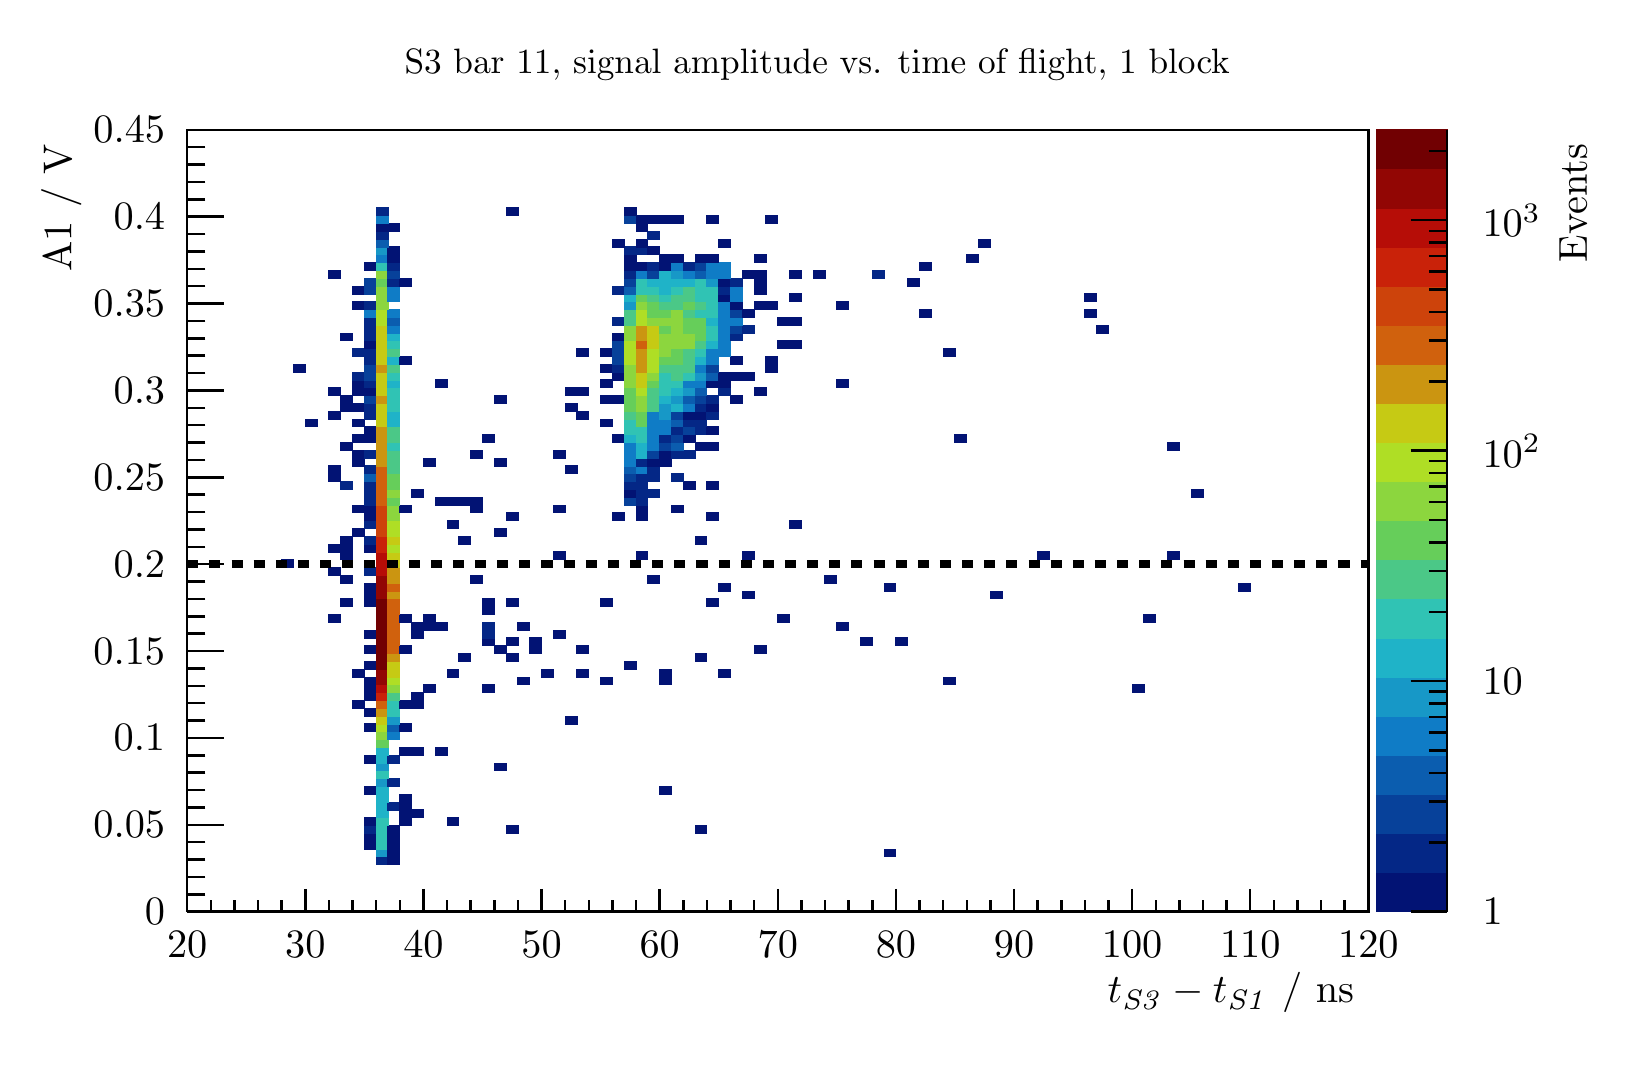
\begin{tikzpicture}
\pgfdeclareplotmark{cross} {
\pgfpathmoveto{\pgfpoint{-0.3\pgfplotmarksize}{\pgfplotmarksize}}
\pgfpathlineto{\pgfpoint{+0.3\pgfplotmarksize}{\pgfplotmarksize}}
\pgfpathlineto{\pgfpoint{+0.3\pgfplotmarksize}{0.3\pgfplotmarksize}}
\pgfpathlineto{\pgfpoint{+1\pgfplotmarksize}{0.3\pgfplotmarksize}}
\pgfpathlineto{\pgfpoint{+1\pgfplotmarksize}{-0.3\pgfplotmarksize}}
\pgfpathlineto{\pgfpoint{+0.3\pgfplotmarksize}{-0.3\pgfplotmarksize}}
\pgfpathlineto{\pgfpoint{+0.3\pgfplotmarksize}{-1.\pgfplotmarksize}}
\pgfpathlineto{\pgfpoint{-0.3\pgfplotmarksize}{-1.\pgfplotmarksize}}
\pgfpathlineto{\pgfpoint{-0.3\pgfplotmarksize}{-0.3\pgfplotmarksize}}
\pgfpathlineto{\pgfpoint{-1.\pgfplotmarksize}{-0.3\pgfplotmarksize}}
\pgfpathlineto{\pgfpoint{-1.\pgfplotmarksize}{0.3\pgfplotmarksize}}
\pgfpathlineto{\pgfpoint{-0.3\pgfplotmarksize}{0.3\pgfplotmarksize}}
\pgfpathclose
\pgfusepathqstroke
}
\pgfdeclareplotmark{cross*} {
\pgfpathmoveto{\pgfpoint{-0.3\pgfplotmarksize}{\pgfplotmarksize}}
\pgfpathlineto{\pgfpoint{+0.3\pgfplotmarksize}{\pgfplotmarksize}}
\pgfpathlineto{\pgfpoint{+0.3\pgfplotmarksize}{0.3\pgfplotmarksize}}
\pgfpathlineto{\pgfpoint{+1\pgfplotmarksize}{0.3\pgfplotmarksize}}
\pgfpathlineto{\pgfpoint{+1\pgfplotmarksize}{-0.3\pgfplotmarksize}}
\pgfpathlineto{\pgfpoint{+0.3\pgfplotmarksize}{-0.3\pgfplotmarksize}}
\pgfpathlineto{\pgfpoint{+0.3\pgfplotmarksize}{-1.\pgfplotmarksize}}
\pgfpathlineto{\pgfpoint{-0.3\pgfplotmarksize}{-1.\pgfplotmarksize}}
\pgfpathlineto{\pgfpoint{-0.3\pgfplotmarksize}{-0.3\pgfplotmarksize}}
\pgfpathlineto{\pgfpoint{-1.\pgfplotmarksize}{-0.3\pgfplotmarksize}}
\pgfpathlineto{\pgfpoint{-1.\pgfplotmarksize}{0.3\pgfplotmarksize}}
\pgfpathlineto{\pgfpoint{-0.3\pgfplotmarksize}{0.3\pgfplotmarksize}}
\pgfpathclose
\pgfusepathqfillstroke
}
\pgfdeclareplotmark{newstar} {
\pgfpathmoveto{\pgfqpoint{0pt}{\pgfplotmarksize}}
\pgfpathlineto{\pgfqpointpolar{44}{0.5\pgfplotmarksize}}
\pgfpathlineto{\pgfqpointpolar{18}{\pgfplotmarksize}}
\pgfpathlineto{\pgfqpointpolar{-20}{0.5\pgfplotmarksize}}
\pgfpathlineto{\pgfqpointpolar{-54}{\pgfplotmarksize}}
\pgfpathlineto{\pgfqpointpolar{-90}{0.5\pgfplotmarksize}}
\pgfpathlineto{\pgfqpointpolar{234}{\pgfplotmarksize}}
\pgfpathlineto{\pgfqpointpolar{198}{0.5\pgfplotmarksize}}
\pgfpathlineto{\pgfqpointpolar{162}{\pgfplotmarksize}}
\pgfpathlineto{\pgfqpointpolar{134}{0.5\pgfplotmarksize}}
\pgfpathclose
\pgfusepathqstroke
}
\pgfdeclareplotmark{newstar*} {
  \pgfpathmoveto{\pgfqpoint{0pt}{\pgfplotmarksize}}
  \pgfpathlineto{\pgfqpointpolar{44}{0.5\pgfplotmarksize}}
  \pgfpathlineto{\pgfqpointpolar{18}{\pgfplotmarksize}}
  \pgfpathlineto{\pgfqpointpolar{-20}{0.5\pgfplotmarksize}}
  \pgfpathlineto{\pgfqpointpolar{-54}{\pgfplotmarksize}}
  \pgfpathlineto{\pgfqpointpolar{-90}{0.5\pgfplotmarksize}}
  \pgfpathlineto{\pgfqpointpolar{234}{\pgfplotmarksize}}
  \pgfpathlineto{\pgfqpointpolar{198}{0.5\pgfplotmarksize}}
  \pgfpathlineto{\pgfqpointpolar{162}{\pgfplotmarksize}}
  \pgfpathlineto{\pgfqpointpolar{134}{0.5\pgfplotmarksize}}
  \pgfpathclose
  \pgfusepathqfillstroke
}
\definecolor{c}{rgb}{1,1,1};
\draw [color=c, fill=c] (0,0) rectangle (20,12.8962);
\draw [color=c, fill=c] (2,1.6765) rectangle (17,11.6066);
\definecolor{c}{rgb}{0,0,0};
\draw [c,line width=0.9] (2,1.6765) -- (2,11.6066) -- (17,11.6066) -- (17,1.6765) -- (2,1.6765);
\definecolor{c}{rgb}{1,1,1};
\draw [color=c, fill=c] (2,1.6765) rectangle (17,11.6066);
\definecolor{c}{rgb}{0,0,0};
\draw [c,line width=0.9] (2,1.6765) -- (2,11.6066) -- (17,11.6066) -- (17,1.6765) -- (2,1.6765);
\definecolor{c}{rgb}{0.0158128,0.151803,0.524225};
\draw [color=c, fill=c] (4.4,2.27231) rectangle (4.55,2.37161);
\definecolor{c}{rgb}{0.00759013,0.0728653,0.45351};
\draw [color=c, fill=c] (4.55,2.27231) rectangle (4.7,2.37161);
\definecolor{c}{rgb}{0.0906863,0.594608,0.78125};
\draw [color=c, fill=c] (4.4,2.37161) rectangle (4.55,2.47091);
\definecolor{c}{rgb}{0.00759013,0.0728653,0.45351};
\draw [color=c, fill=c] (4.55,2.37161) rectangle (4.7,2.47091);
\draw [color=c, fill=c] (10.85,2.37161) rectangle (11,2.47091);
\draw [color=c, fill=c] (4.25,2.47091) rectangle (4.4,2.57021);
\definecolor{c}{rgb}{0.18652,0.763235,0.706618};
\draw [color=c, fill=c] (4.4,2.47091) rectangle (4.55,2.57021);
\definecolor{c}{rgb}{0.00759013,0.0728653,0.45351};
\draw [color=c, fill=c] (4.55,2.47091) rectangle (4.7,2.57021);
\draw [color=c, fill=c] (4.25,2.57021) rectangle (4.4,2.66951);
\definecolor{c}{rgb}{0.18652,0.763235,0.706618};
\draw [color=c, fill=c] (4.4,2.57021) rectangle (4.55,2.66951);
\definecolor{c}{rgb}{0.00759013,0.0728653,0.45351};
\draw [color=c, fill=c] (4.55,2.57021) rectangle (4.7,2.66951);
\definecolor{c}{rgb}{0.0158128,0.151803,0.524225};
\draw [color=c, fill=c] (4.25,2.66951) rectangle (4.4,2.76881);
\definecolor{c}{rgb}{0.18652,0.763235,0.706618};
\draw [color=c, fill=c] (4.4,2.66951) rectangle (4.55,2.76881);
\definecolor{c}{rgb}{0.00759013,0.0728653,0.45351};
\draw [color=c, fill=c] (4.55,2.66951) rectangle (4.7,2.76881);
\draw [color=c, fill=c] (6.05,2.66951) rectangle (6.2,2.76881);
\draw [color=c, fill=c] (8.45,2.66951) rectangle (8.6,2.76881);
\draw [color=c, fill=c] (4.25,2.76881) rectangle (4.4,2.86811);
\definecolor{c}{rgb}{0.18652,0.763235,0.706618};
\draw [color=c, fill=c] (4.4,2.76881) rectangle (4.55,2.86811);
\definecolor{c}{rgb}{0.00759013,0.0728653,0.45351};
\draw [color=c, fill=c] (4.7,2.76881) rectangle (4.85,2.86811);
\draw [color=c, fill=c] (5.3,2.76881) rectangle (5.45,2.86811);
\definecolor{c}{rgb}{0.122549,0.702941,0.786029};
\draw [color=c, fill=c] (4.4,2.86811) rectangle (4.55,2.96741);
\definecolor{c}{rgb}{0.00759013,0.0728653,0.45351};
\draw [color=c, fill=c] (4.7,2.86811) rectangle (4.85,2.96741);
\draw [color=c, fill=c] (4.85,2.86811) rectangle (5,2.96741);
\definecolor{c}{rgb}{0.122549,0.702941,0.786029};
\draw [color=c, fill=c] (4.4,2.96741) rectangle (4.55,3.06671);
\definecolor{c}{rgb}{0.0158128,0.151803,0.524225};
\draw [color=c, fill=c] (4.55,2.96741) rectangle (4.7,3.06671);
\definecolor{c}{rgb}{0.00759013,0.0728653,0.45351};
\draw [color=c, fill=c] (4.7,2.96741) rectangle (4.85,3.06671);
\definecolor{c}{rgb}{0.122549,0.702941,0.786029};
\draw [color=c, fill=c] (4.4,3.06671) rectangle (4.55,3.16601);
\definecolor{c}{rgb}{0.00759013,0.0728653,0.45351};
\draw [color=c, fill=c] (4.7,3.06671) rectangle (4.85,3.16601);
\draw [color=c, fill=c] (4.25,3.16601) rectangle (4.4,3.26531);
\definecolor{c}{rgb}{0.122549,0.702941,0.786029};
\draw [color=c, fill=c] (4.4,3.16601) rectangle (4.55,3.26531);
\definecolor{c}{rgb}{0.00759013,0.0728653,0.45351};
\draw [color=c, fill=c] (8,3.16601) rectangle (8.15,3.26531);
\definecolor{c}{rgb}{0.0906863,0.594608,0.78125};
\draw [color=c, fill=c] (4.4,3.26531) rectangle (4.55,3.36461);
\definecolor{c}{rgb}{0.0158128,0.151803,0.524225};
\draw [color=c, fill=c] (4.55,3.26531) rectangle (4.7,3.36461);
\definecolor{c}{rgb}{0.18652,0.763235,0.706618};
\draw [color=c, fill=c] (4.4,3.36461) rectangle (4.55,3.46391);
\definecolor{c}{rgb}{0.0906863,0.594608,0.78125};
\draw [color=c, fill=c] (4.4,3.46391) rectangle (4.55,3.56321);
\definecolor{c}{rgb}{0.00759013,0.0728653,0.45351};
\draw [color=c, fill=c] (5.9,3.46391) rectangle (6.05,3.56321);
\draw [color=c, fill=c] (4.25,3.56321) rectangle (4.4,3.66251);
\definecolor{c}{rgb}{0.122549,0.702941,0.786029};
\draw [color=c, fill=c] (4.4,3.56321) rectangle (4.55,3.66251);
\definecolor{c}{rgb}{0.0158128,0.151803,0.524225};
\draw [color=c, fill=c] (4.55,3.56321) rectangle (4.7,3.66251);
\definecolor{c}{rgb}{0.122549,0.702941,0.786029};
\draw [color=c, fill=c] (4.4,3.66251) rectangle (4.55,3.76181);
\definecolor{c}{rgb}{0.00759013,0.0728653,0.45351};
\draw [color=c, fill=c] (4.7,3.66251) rectangle (4.85,3.76181);
\draw [color=c, fill=c] (4.85,3.66251) rectangle (5,3.76181);
\draw [color=c, fill=c] (5.15,3.66251) rectangle (5.3,3.76181);
\definecolor{c}{rgb}{0.4,0.807843,0.352941};
\draw [color=c, fill=c] (4.4,3.76181) rectangle (4.55,3.86111);
\definecolor{c}{rgb}{0.549755,0.839706,0.244608};
\draw [color=c, fill=c] (4.4,3.86111) rectangle (4.55,3.96042);
\definecolor{c}{rgb}{0.0588235,0.486275,0.776471};
\draw [color=c, fill=c] (4.55,3.86111) rectangle (4.7,3.96042);
\definecolor{c}{rgb}{0.00759013,0.0728653,0.45351};
\draw [color=c, fill=c] (4.25,3.96042) rectangle (4.4,4.05972);
\definecolor{c}{rgb}{0.68799,0.869118,0.144608};
\draw [color=c, fill=c] (4.4,3.96042) rectangle (4.55,4.05972);
\definecolor{c}{rgb}{0.0428922,0.365196,0.687255};
\draw [color=c, fill=c] (4.55,3.96042) rectangle (4.7,4.05972);
\definecolor{c}{rgb}{0.00759013,0.0728653,0.45351};
\draw [color=c, fill=c] (4.7,3.96042) rectangle (4.85,4.05972);
\definecolor{c}{rgb}{0.777451,0.791422,0.0796569};
\draw [color=c, fill=c] (4.4,4.05972) rectangle (4.55,4.15902);
\definecolor{c}{rgb}{0.0906863,0.594608,0.78125};
\draw [color=c, fill=c] (4.55,4.05972) rectangle (4.7,4.15902);
\definecolor{c}{rgb}{0.00759013,0.0728653,0.45351};
\draw [color=c, fill=c] (6.8,4.05972) rectangle (6.95,4.15902);
\draw [color=c, fill=c] (4.25,4.15902) rectangle (4.4,4.25832);
\definecolor{c}{rgb}{0.796569,0.585907,0.0653186};
\draw [color=c, fill=c] (4.4,4.15902) rectangle (4.55,4.25832);
\definecolor{c}{rgb}{0.18652,0.763235,0.706618};
\draw [color=c, fill=c] (4.55,4.15902) rectangle (4.7,4.25832);
\definecolor{c}{rgb}{0.00759013,0.0728653,0.45351};
\draw [color=c, fill=c] (4.1,4.25832) rectangle (4.25,4.35762);
\definecolor{c}{rgb}{0.815686,0.380392,0.0509804};
\draw [color=c, fill=c] (4.4,4.25832) rectangle (4.55,4.35762);
\definecolor{c}{rgb}{0.18652,0.763235,0.706618};
\draw [color=c, fill=c] (4.55,4.25832) rectangle (4.7,4.35762);
\definecolor{c}{rgb}{0.00759013,0.0728653,0.45351};
\draw [color=c, fill=c] (4.7,4.25832) rectangle (4.85,4.35762);
\draw [color=c, fill=c] (4.85,4.25832) rectangle (5,4.35762);
\draw [color=c, fill=c] (4.25,4.35762) rectangle (4.4,4.45692);
\definecolor{c}{rgb}{0.788113,0.13223,0.0356618};
\draw [color=c, fill=c] (4.4,4.35762) rectangle (4.55,4.45692);
\definecolor{c}{rgb}{0.29326,0.785539,0.529779};
\draw [color=c, fill=c] (4.55,4.35762) rectangle (4.7,4.45692);
\definecolor{c}{rgb}{0.00759013,0.0728653,0.45351};
\draw [color=c, fill=c] (4.85,4.35762) rectangle (5,4.45692);
\draw [color=c, fill=c] (4.25,4.45692) rectangle (4.4,4.55622);
\definecolor{c}{rgb}{0.714951,0.0509804,0.0269608};
\draw [color=c, fill=c] (4.4,4.45692) rectangle (4.55,4.55622);
\definecolor{c}{rgb}{0.549755,0.839706,0.244608};
\draw [color=c, fill=c] (4.55,4.45692) rectangle (4.7,4.55622);
\definecolor{c}{rgb}{0.00759013,0.0728653,0.45351};
\draw [color=c, fill=c] (5,4.45692) rectangle (5.15,4.55622);
\draw [color=c, fill=c] (5.75,4.45692) rectangle (5.9,4.55622);
\draw [color=c, fill=c] (14,4.45692) rectangle (14.15,4.55622);
\draw [color=c, fill=c] (4.25,4.55622) rectangle (4.4,4.65552);
\definecolor{c}{rgb}{0.573162,0.0254902,0.017402};
\draw [color=c, fill=c] (4.4,4.55622) rectangle (4.55,4.65552);
\definecolor{c}{rgb}{0.68799,0.869118,0.144608};
\draw [color=c, fill=c] (4.55,4.55622) rectangle (4.7,4.65552);
\definecolor{c}{rgb}{0.00759013,0.0728653,0.45351};
\draw [color=c, fill=c] (6.2,4.55622) rectangle (6.35,4.65552);
\draw [color=c, fill=c] (7.25,4.55622) rectangle (7.4,4.65552);
\draw [color=c, fill=c] (8,4.55622) rectangle (8.15,4.65552);
\draw [color=c, fill=c] (11.6,4.55622) rectangle (11.75,4.65552);
\draw [color=c, fill=c] (4.1,4.65552) rectangle (4.25,4.75482);
\definecolor{c}{rgb}{0.573162,0.0254902,0.017402};
\draw [color=c, fill=c] (4.4,4.65552) rectangle (4.55,4.75482);
\definecolor{c}{rgb}{0.777451,0.791422,0.0796569};
\draw [color=c, fill=c] (4.55,4.65552) rectangle (4.7,4.75482);
\definecolor{c}{rgb}{0.00759013,0.0728653,0.45351};
\draw [color=c, fill=c] (5.3,4.65552) rectangle (5.45,4.75482);
\draw [color=c, fill=c] (6.5,4.65552) rectangle (6.65,4.75482);
\draw [color=c, fill=c] (6.95,4.65552) rectangle (7.1,4.75482);
\draw [color=c, fill=c] (8,4.65552) rectangle (8.15,4.75482);
\draw [color=c, fill=c] (8.75,4.65552) rectangle (8.9,4.75482);
\draw [color=c, fill=c] (4.25,4.75482) rectangle (4.4,4.85412);
\definecolor{c}{rgb}{0.442279,0.00196078,0.00857843};
\draw [color=c, fill=c] (4.4,4.75482) rectangle (4.55,4.85412);
\definecolor{c}{rgb}{0.777451,0.791422,0.0796569};
\draw [color=c, fill=c] (4.55,4.75482) rectangle (4.7,4.85412);
\definecolor{c}{rgb}{0.00759013,0.0728653,0.45351};
\draw [color=c, fill=c] (7.55,4.75482) rectangle (7.7,4.85412);
\definecolor{c}{rgb}{0.442279,0.00196078,0.00857843};
\draw [color=c, fill=c] (4.4,4.85412) rectangle (4.55,4.95342);
\definecolor{c}{rgb}{0.796569,0.585907,0.0653186};
\draw [color=c, fill=c] (4.55,4.85412) rectangle (4.7,4.95342);
\definecolor{c}{rgb}{0.00759013,0.0728653,0.45351};
\draw [color=c, fill=c] (5.45,4.85412) rectangle (5.6,4.95342);
\draw [color=c, fill=c] (6.05,4.85412) rectangle (6.2,4.95342);
\draw [color=c, fill=c] (8.45,4.85412) rectangle (8.6,4.95342);
\draw [color=c, fill=c] (4.25,4.95342) rectangle (4.4,5.05272);
\definecolor{c}{rgb}{0.442279,0.00196078,0.00857843};
\draw [color=c, fill=c] (4.4,4.95342) rectangle (4.55,5.05272);
\definecolor{c}{rgb}{0.815686,0.380392,0.0509804};
\draw [color=c, fill=c] (4.55,4.95342) rectangle (4.7,5.05272);
\definecolor{c}{rgb}{0.00759013,0.0728653,0.45351};
\draw [color=c, fill=c] (4.7,4.95342) rectangle (4.85,5.05272);
\draw [color=c, fill=c] (5.9,4.95342) rectangle (6.05,5.05272);
\draw [color=c, fill=c] (6.35,4.95342) rectangle (6.5,5.05272);
\draw [color=c, fill=c] (6.95,4.95342) rectangle (7.1,5.05272);
\draw [color=c, fill=c] (9.2,4.95342) rectangle (9.35,5.05272);
\definecolor{c}{rgb}{0.442279,0.00196078,0.00857843};
\draw [color=c, fill=c] (4.4,5.05272) rectangle (4.55,5.15202);
\definecolor{c}{rgb}{0.815686,0.380392,0.0509804};
\draw [color=c, fill=c] (4.55,5.05272) rectangle (4.7,5.15202);
\definecolor{c}{rgb}{0.00759013,0.0728653,0.45351};
\draw [color=c, fill=c] (5.75,5.05272) rectangle (5.9,5.15202);
\draw [color=c, fill=c] (6.05,5.05272) rectangle (6.2,5.15202);
\draw [color=c, fill=c] (6.35,5.05272) rectangle (6.5,5.15202);
\draw [color=c, fill=c] (10.55,5.05272) rectangle (10.7,5.15202);
\draw [color=c, fill=c] (11,5.05272) rectangle (11.15,5.15202);
\draw [color=c, fill=c] (4.25,5.15202) rectangle (4.4,5.25132);
\definecolor{c}{rgb}{0.442279,0.00196078,0.00857843};
\draw [color=c, fill=c] (4.4,5.15202) rectangle (4.55,5.25132);
\definecolor{c}{rgb}{0.815686,0.380392,0.0509804};
\draw [color=c, fill=c] (4.55,5.15202) rectangle (4.7,5.25132);
\definecolor{c}{rgb}{0.00759013,0.0728653,0.45351};
\draw [color=c, fill=c] (4.85,5.15202) rectangle (5,5.25132);
\definecolor{c}{rgb}{0.0158128,0.151803,0.524225};
\draw [color=c, fill=c] (5.75,5.15202) rectangle (5.9,5.25132);
\definecolor{c}{rgb}{0.00759013,0.0728653,0.45351};
\draw [color=c, fill=c] (6.65,5.15202) rectangle (6.8,5.25132);
\definecolor{c}{rgb}{0.442279,0.00196078,0.00857843};
\draw [color=c, fill=c] (4.4,5.25132) rectangle (4.55,5.35062);
\definecolor{c}{rgb}{0.815686,0.380392,0.0509804};
\draw [color=c, fill=c] (4.55,5.25132) rectangle (4.7,5.35062);
\definecolor{c}{rgb}{0.00759013,0.0728653,0.45351};
\draw [color=c, fill=c] (4.85,5.25132) rectangle (5,5.35062);
\draw [color=c, fill=c] (5,5.25132) rectangle (5.15,5.35062);
\draw [color=c, fill=c] (5.15,5.25132) rectangle (5.3,5.35062);
\definecolor{c}{rgb}{0.0158128,0.151803,0.524225};
\draw [color=c, fill=c] (5.75,5.25132) rectangle (5.9,5.35062);
\definecolor{c}{rgb}{0.00759013,0.0728653,0.45351};
\draw [color=c, fill=c] (6.2,5.25132) rectangle (6.35,5.35062);
\draw [color=c, fill=c] (10.25,5.25132) rectangle (10.4,5.35062);
\draw [color=c, fill=c] (3.8,5.35062) rectangle (3.95,5.44992);
\definecolor{c}{rgb}{0.442279,0.00196078,0.00857843};
\draw [color=c, fill=c] (4.4,5.35062) rectangle (4.55,5.44992);
\definecolor{c}{rgb}{0.815686,0.380392,0.0509804};
\draw [color=c, fill=c] (4.55,5.35062) rectangle (4.7,5.44992);
\definecolor{c}{rgb}{0.00759013,0.0728653,0.45351};
\draw [color=c, fill=c] (4.7,5.35062) rectangle (4.85,5.44992);
\draw [color=c, fill=c] (5,5.35062) rectangle (5.15,5.44992);
\draw [color=c, fill=c] (9.5,5.35062) rectangle (9.65,5.44992);
\draw [color=c, fill=c] (14.15,5.35062) rectangle (14.3,5.44992);
\definecolor{c}{rgb}{0.442279,0.00196078,0.00857843};
\draw [color=c, fill=c] (4.4,5.44992) rectangle (4.55,5.54922);
\definecolor{c}{rgb}{0.815686,0.380392,0.0509804};
\draw [color=c, fill=c] (4.55,5.44992) rectangle (4.7,5.54922);
\definecolor{c}{rgb}{0.00759013,0.0728653,0.45351};
\draw [color=c, fill=c] (5.75,5.44992) rectangle (5.9,5.54922);
\draw [color=c, fill=c] (3.95,5.54922) rectangle (4.1,5.64852);
\draw [color=c, fill=c] (4.25,5.54922) rectangle (4.4,5.64852);
\definecolor{c}{rgb}{0.442279,0.00196078,0.00857843};
\draw [color=c, fill=c] (4.4,5.54922) rectangle (4.55,5.64852);
\definecolor{c}{rgb}{0.815686,0.380392,0.0509804};
\draw [color=c, fill=c] (4.55,5.54922) rectangle (4.7,5.64852);
\definecolor{c}{rgb}{0.00759013,0.0728653,0.45351};
\draw [color=c, fill=c] (5.75,5.54922) rectangle (5.9,5.64852);
\draw [color=c, fill=c] (6.05,5.54922) rectangle (6.2,5.64852);
\draw [color=c, fill=c] (7.25,5.54922) rectangle (7.4,5.64852);
\draw [color=c, fill=c] (8.6,5.54922) rectangle (8.75,5.64852);
\draw [color=c, fill=c] (4.25,5.64852) rectangle (4.4,5.74783);
\definecolor{c}{rgb}{0.573162,0.0254902,0.017402};
\draw [color=c, fill=c] (4.4,5.64852) rectangle (4.55,5.74783);
\definecolor{c}{rgb}{0.796569,0.585907,0.0653186};
\draw [color=c, fill=c] (4.55,5.64852) rectangle (4.7,5.74783);
\definecolor{c}{rgb}{0.00759013,0.0728653,0.45351};
\draw [color=c, fill=c] (9.05,5.64852) rectangle (9.2,5.74783);
\draw [color=c, fill=c] (12.2,5.64852) rectangle (12.35,5.74783);
\draw [color=c, fill=c] (4.25,5.74783) rectangle (4.4,5.84713);
\definecolor{c}{rgb}{0.573162,0.0254902,0.017402};
\draw [color=c, fill=c] (4.4,5.74783) rectangle (4.55,5.84713);
\definecolor{c}{rgb}{0.815686,0.380392,0.0509804};
\draw [color=c, fill=c] (4.55,5.74783) rectangle (4.7,5.84713);
\definecolor{c}{rgb}{0.00759013,0.0728653,0.45351};
\draw [color=c, fill=c] (8.75,5.74783) rectangle (8.9,5.84713);
\draw [color=c, fill=c] (10.85,5.74783) rectangle (11,5.84713);
\draw [color=c, fill=c] (15.35,5.74783) rectangle (15.5,5.84713);
\draw [color=c, fill=c] (3.95,5.84713) rectangle (4.1,5.94643);
\definecolor{c}{rgb}{0.573162,0.0254902,0.017402};
\draw [color=c, fill=c] (4.4,5.84713) rectangle (4.55,5.94643);
\definecolor{c}{rgb}{0.796569,0.585907,0.0653186};
\draw [color=c, fill=c] (4.55,5.84713) rectangle (4.7,5.94643);
\definecolor{c}{rgb}{0.00759013,0.0728653,0.45351};
\draw [color=c, fill=c] (5.6,5.84713) rectangle (5.75,5.94643);
\draw [color=c, fill=c] (7.85,5.84713) rectangle (8,5.94643);
\draw [color=c, fill=c] (10.1,5.84713) rectangle (10.25,5.94643);
\draw [color=c, fill=c] (3.8,5.94643) rectangle (3.95,6.04573);
\definecolor{c}{rgb}{0.0158128,0.151803,0.524225};
\draw [color=c, fill=c] (4.25,5.94643) rectangle (4.4,6.04573);
\definecolor{c}{rgb}{0.714951,0.0509804,0.0269608};
\draw [color=c, fill=c] (4.4,5.94643) rectangle (4.55,6.04573);
\definecolor{c}{rgb}{0.796569,0.585907,0.0653186};
\draw [color=c, fill=c] (4.55,5.94643) rectangle (4.7,6.04573);
\definecolor{c}{rgb}{0.00759013,0.0728653,0.45351};
\draw [color=c, fill=c] (3.2,6.04573) rectangle (3.35,6.14503);
\definecolor{c}{rgb}{0.714951,0.0509804,0.0269608};
\draw [color=c, fill=c] (4.4,6.04573) rectangle (4.55,6.14503);
\definecolor{c}{rgb}{0.777451,0.791422,0.0796569};
\draw [color=c, fill=c] (4.55,6.04573) rectangle (4.7,6.14503);
\definecolor{c}{rgb}{0.00759013,0.0728653,0.45351};
\draw [color=c, fill=c] (3.95,6.14503) rectangle (4.1,6.24433);
\definecolor{c}{rgb}{0.714951,0.0509804,0.0269608};
\draw [color=c, fill=c] (4.4,6.14503) rectangle (4.55,6.24433);
\definecolor{c}{rgb}{0.777451,0.791422,0.0796569};
\draw [color=c, fill=c] (4.55,6.14503) rectangle (4.7,6.24433);
\definecolor{c}{rgb}{0.00759013,0.0728653,0.45351};
\draw [color=c, fill=c] (6.65,6.14503) rectangle (6.8,6.24433);
\draw [color=c, fill=c] (7.7,6.14503) rectangle (7.85,6.24433);
\draw [color=c, fill=c] (9.05,6.14503) rectangle (9.2,6.24433);
\draw [color=c, fill=c] (12.8,6.14503) rectangle (12.95,6.24433);
\draw [color=c, fill=c] (14.45,6.14503) rectangle (14.6,6.24433);
\draw [color=c, fill=c] (3.8,6.24433) rectangle (3.95,6.34363);
\draw [color=c, fill=c] (3.95,6.24433) rectangle (4.1,6.34363);
\draw [color=c, fill=c] (4.25,6.24433) rectangle (4.4,6.34363);
\definecolor{c}{rgb}{0.788113,0.13223,0.0356618};
\draw [color=c, fill=c] (4.4,6.24433) rectangle (4.55,6.34363);
\definecolor{c}{rgb}{0.68799,0.869118,0.144608};
\draw [color=c, fill=c] (4.55,6.24433) rectangle (4.7,6.34363);
\definecolor{c}{rgb}{0.00759013,0.0728653,0.45351};
\draw [color=c, fill=c] (3.95,6.34363) rectangle (4.1,6.44293);
\definecolor{c}{rgb}{0.0158128,0.151803,0.524225};
\draw [color=c, fill=c] (4.25,6.34363) rectangle (4.4,6.44293);
\definecolor{c}{rgb}{0.788113,0.13223,0.0356618};
\draw [color=c, fill=c] (4.4,6.34363) rectangle (4.55,6.44293);
\definecolor{c}{rgb}{0.777451,0.791422,0.0796569};
\draw [color=c, fill=c] (4.55,6.34363) rectangle (4.7,6.44293);
\definecolor{c}{rgb}{0.00759013,0.0728653,0.45351};
\draw [color=c, fill=c] (5.45,6.34363) rectangle (5.6,6.44293);
\draw [color=c, fill=c] (8.45,6.34363) rectangle (8.6,6.44293);
\draw [color=c, fill=c] (4.1,6.44293) rectangle (4.25,6.54223);
\definecolor{c}{rgb}{0.802451,0.261275,0.0436275};
\draw [color=c, fill=c] (4.4,6.44293) rectangle (4.55,6.54223);
\definecolor{c}{rgb}{0.68799,0.869118,0.144608};
\draw [color=c, fill=c] (4.55,6.44293) rectangle (4.7,6.54223);
\definecolor{c}{rgb}{0.00759013,0.0728653,0.45351};
\draw [color=c, fill=c] (5.9,6.44293) rectangle (6.05,6.54223);
\definecolor{c}{rgb}{0.0158128,0.151803,0.524225};
\draw [color=c, fill=c] (4.25,6.54223) rectangle (4.4,6.64153);
\definecolor{c}{rgb}{0.802451,0.261275,0.0436275};
\draw [color=c, fill=c] (4.4,6.54223) rectangle (4.55,6.64153);
\definecolor{c}{rgb}{0.68799,0.869118,0.144608};
\draw [color=c, fill=c] (4.55,6.54223) rectangle (4.7,6.64153);
\definecolor{c}{rgb}{0.00759013,0.0728653,0.45351};
\draw [color=c, fill=c] (5.3,6.54223) rectangle (5.45,6.64153);
\draw [color=c, fill=c] (9.65,6.54223) rectangle (9.8,6.64153);
\draw [color=c, fill=c] (4.25,6.64153) rectangle (4.4,6.74083);
\definecolor{c}{rgb}{0.802451,0.261275,0.0436275};
\draw [color=c, fill=c] (4.4,6.64153) rectangle (4.55,6.74083);
\definecolor{c}{rgb}{0.549755,0.839706,0.244608};
\draw [color=c, fill=c] (4.55,6.64153) rectangle (4.7,6.74083);
\definecolor{c}{rgb}{0.00759013,0.0728653,0.45351};
\draw [color=c, fill=c] (6.05,6.64153) rectangle (6.2,6.74083);
\draw [color=c, fill=c] (7.4,6.64153) rectangle (7.55,6.74083);
\draw [color=c, fill=c] (7.7,6.64153) rectangle (7.85,6.74083);
\draw [color=c, fill=c] (8.6,6.64153) rectangle (8.75,6.74083);
\draw [color=c, fill=c] (4.1,6.74083) rectangle (4.25,6.84013);
\draw [color=c, fill=c] (4.25,6.74083) rectangle (4.4,6.84013);
\definecolor{c}{rgb}{0.802451,0.261275,0.0436275};
\draw [color=c, fill=c] (4.4,6.74083) rectangle (4.55,6.84013);
\definecolor{c}{rgb}{0.549755,0.839706,0.244608};
\draw [color=c, fill=c] (4.55,6.74083) rectangle (4.7,6.84013);
\definecolor{c}{rgb}{0.00759013,0.0728653,0.45351};
\draw [color=c, fill=c] (4.7,6.74083) rectangle (4.85,6.84013);
\draw [color=c, fill=c] (5.6,6.74083) rectangle (5.75,6.84013);
\draw [color=c, fill=c] (6.65,6.74083) rectangle (6.8,6.84013);
\draw [color=c, fill=c] (7.7,6.74083) rectangle (7.85,6.84013);
\draw [color=c, fill=c] (8.15,6.74083) rectangle (8.3,6.84013);
\definecolor{c}{rgb}{0.0158128,0.151803,0.524225};
\draw [color=c, fill=c] (4.25,6.84013) rectangle (4.4,6.93943);
\definecolor{c}{rgb}{0.815686,0.380392,0.0509804};
\draw [color=c, fill=c] (4.4,6.84013) rectangle (4.55,6.93943);
\definecolor{c}{rgb}{0.4,0.807843,0.352941};
\draw [color=c, fill=c] (4.55,6.84013) rectangle (4.7,6.93943);
\definecolor{c}{rgb}{0.00759013,0.0728653,0.45351};
\draw [color=c, fill=c] (5.15,6.84013) rectangle (5.3,6.93943);
\draw [color=c, fill=c] (5.3,6.84013) rectangle (5.45,6.93943);
\draw [color=c, fill=c] (5.45,6.84013) rectangle (5.6,6.93943);
\draw [color=c, fill=c] (5.6,6.84013) rectangle (5.75,6.93943);
\definecolor{c}{rgb}{0.0281863,0.253431,0.604902};
\draw [color=c, fill=c] (7.55,6.84013) rectangle (7.7,6.93943);
\definecolor{c}{rgb}{0.0158128,0.151803,0.524225};
\draw [color=c, fill=c] (7.7,6.84013) rectangle (7.85,6.93943);
\draw [color=c, fill=c] (4.25,6.93943) rectangle (4.4,7.03873);
\definecolor{c}{rgb}{0.815686,0.380392,0.0509804};
\draw [color=c, fill=c] (4.4,6.93943) rectangle (4.55,7.03873);
\definecolor{c}{rgb}{0.549755,0.839706,0.244608};
\draw [color=c, fill=c] (4.55,6.93943) rectangle (4.7,7.03873);
\definecolor{c}{rgb}{0.00759013,0.0728653,0.45351};
\draw [color=c, fill=c] (4.85,6.93943) rectangle (5,7.03873);
\draw [color=c, fill=c] (7.55,6.93943) rectangle (7.7,7.03873);
\definecolor{c}{rgb}{0.0158128,0.151803,0.524225};
\draw [color=c, fill=c] (7.7,6.93943) rectangle (7.85,7.03873);
\draw [color=c, fill=c] (7.85,6.93943) rectangle (8,7.03873);
\definecolor{c}{rgb}{0.00759013,0.0728653,0.45351};
\draw [color=c, fill=c] (14.75,6.93943) rectangle (14.9,7.03873);
\definecolor{c}{rgb}{0.0158128,0.151803,0.524225};
\draw [color=c, fill=c] (3.95,7.03873) rectangle (4.1,7.13803);
\draw [color=c, fill=c] (4.25,7.03873) rectangle (4.4,7.13803);
\definecolor{c}{rgb}{0.815686,0.380392,0.0509804};
\draw [color=c, fill=c] (4.4,7.03873) rectangle (4.55,7.13803);
\definecolor{c}{rgb}{0.4,0.807843,0.352941};
\draw [color=c, fill=c] (4.55,7.03873) rectangle (4.7,7.13803);
\definecolor{c}{rgb}{0.0158128,0.151803,0.524225};
\draw [color=c, fill=c] (7.55,7.03873) rectangle (7.7,7.13803);
\draw [color=c, fill=c] (7.7,7.03873) rectangle (7.85,7.13803);
\definecolor{c}{rgb}{0.00759013,0.0728653,0.45351};
\draw [color=c, fill=c] (8.3,7.03873) rectangle (8.45,7.13803);
\draw [color=c, fill=c] (8.6,7.03873) rectangle (8.75,7.13803);
\draw [color=c, fill=c] (3.8,7.13803) rectangle (3.95,7.23733);
\definecolor{c}{rgb}{0.0428922,0.365196,0.687255};
\draw [color=c, fill=c] (4.25,7.13803) rectangle (4.4,7.23733);
\definecolor{c}{rgb}{0.815686,0.380392,0.0509804};
\draw [color=c, fill=c] (4.4,7.13803) rectangle (4.55,7.23733);
\definecolor{c}{rgb}{0.4,0.807843,0.352941};
\draw [color=c, fill=c] (4.55,7.13803) rectangle (4.7,7.23733);
\definecolor{c}{rgb}{0.0281863,0.253431,0.604902};
\draw [color=c, fill=c] (7.55,7.13803) rectangle (7.7,7.23733);
\definecolor{c}{rgb}{0.0158128,0.151803,0.524225};
\draw [color=c, fill=c] (7.7,7.13803) rectangle (7.85,7.23733);
\draw [color=c, fill=c] (7.85,7.13803) rectangle (8,7.23733);
\draw [color=c, fill=c] (8.15,7.13803) rectangle (8.3,7.23733);
\definecolor{c}{rgb}{0.00759013,0.0728653,0.45351};
\draw [color=c, fill=c] (3.8,7.23733) rectangle (3.95,7.33663);
\definecolor{c}{rgb}{0.0158128,0.151803,0.524225};
\draw [color=c, fill=c] (4.25,7.23733) rectangle (4.4,7.33663);
\definecolor{c}{rgb}{0.815686,0.380392,0.0509804};
\draw [color=c, fill=c] (4.4,7.23733) rectangle (4.55,7.33663);
\definecolor{c}{rgb}{0.29326,0.785539,0.529779};
\draw [color=c, fill=c] (4.55,7.23733) rectangle (4.7,7.33663);
\definecolor{c}{rgb}{0.00759013,0.0728653,0.45351};
\draw [color=c, fill=c] (6.8,7.23733) rectangle (6.95,7.33663);
\definecolor{c}{rgb}{0.0428922,0.365196,0.687255};
\draw [color=c, fill=c] (7.55,7.23733) rectangle (7.7,7.33663);
\definecolor{c}{rgb}{0.0588235,0.486275,0.776471};
\draw [color=c, fill=c] (7.7,7.23733) rectangle (7.85,7.33663);
\definecolor{c}{rgb}{0.0158128,0.151803,0.524225};
\draw [color=c, fill=c] (7.85,7.23733) rectangle (8,7.33663);
\definecolor{c}{rgb}{0.00759013,0.0728653,0.45351};
\draw [color=c, fill=c] (4.1,7.33663) rectangle (4.25,7.43593);
\definecolor{c}{rgb}{0.796569,0.585907,0.0653186};
\draw [color=c, fill=c] (4.4,7.33663) rectangle (4.55,7.43593);
\definecolor{c}{rgb}{0.29326,0.785539,0.529779};
\draw [color=c, fill=c] (4.55,7.33663) rectangle (4.7,7.43593);
\definecolor{c}{rgb}{0.00759013,0.0728653,0.45351};
\draw [color=c, fill=c] (5,7.33663) rectangle (5.15,7.43593);
\draw [color=c, fill=c] (5.9,7.33663) rectangle (6.05,7.43593);
\definecolor{c}{rgb}{0.0588235,0.486275,0.776471};
\draw [color=c, fill=c] (7.55,7.33663) rectangle (7.7,7.43593);
\definecolor{c}{rgb}{0.0158128,0.151803,0.524225};
\draw [color=c, fill=c] (7.7,7.33663) rectangle (7.85,7.43593);
\definecolor{c}{rgb}{0.00759013,0.0728653,0.45351};
\draw [color=c, fill=c] (7.85,7.33663) rectangle (8,7.43593);
\draw [color=c, fill=c] (8,7.33663) rectangle (8.15,7.43593);
\draw [color=c, fill=c] (4.1,7.43593) rectangle (4.25,7.53523);
\definecolor{c}{rgb}{0.0158128,0.151803,0.524225};
\draw [color=c, fill=c] (4.25,7.43593) rectangle (4.4,7.53523);
\definecolor{c}{rgb}{0.796569,0.585907,0.0653186};
\draw [color=c, fill=c] (4.4,7.43593) rectangle (4.55,7.53523);
\definecolor{c}{rgb}{0.29326,0.785539,0.529779};
\draw [color=c, fill=c] (4.55,7.43593) rectangle (4.7,7.53523);
\definecolor{c}{rgb}{0.00759013,0.0728653,0.45351};
\draw [color=c, fill=c] (5.6,7.43593) rectangle (5.75,7.53523);
\draw [color=c, fill=c] (6.65,7.43593) rectangle (6.8,7.53523);
\definecolor{c}{rgb}{0.0588235,0.486275,0.776471};
\draw [color=c, fill=c] (7.55,7.43593) rectangle (7.7,7.53523);
\definecolor{c}{rgb}{0.122549,0.702941,0.786029};
\draw [color=c, fill=c] (7.7,7.43593) rectangle (7.85,7.53523);
\definecolor{c}{rgb}{0.0281863,0.253431,0.604902};
\draw [color=c, fill=c] (7.85,7.43593) rectangle (8,7.53523);
\definecolor{c}{rgb}{0.00759013,0.0728653,0.45351};
\draw [color=c, fill=c] (8,7.43593) rectangle (8.15,7.53523);
\definecolor{c}{rgb}{0.0158128,0.151803,0.524225};
\draw [color=c, fill=c] (8.15,7.43593) rectangle (8.3,7.53523);
\draw [color=c, fill=c] (8.3,7.43593) rectangle (8.45,7.53523);
\definecolor{c}{rgb}{0.00759013,0.0728653,0.45351};
\draw [color=c, fill=c] (3.95,7.53523) rectangle (4.1,7.63454);
\definecolor{c}{rgb}{0.796569,0.585907,0.0653186};
\draw [color=c, fill=c] (4.4,7.53523) rectangle (4.55,7.63454);
\definecolor{c}{rgb}{0.18652,0.763235,0.706618};
\draw [color=c, fill=c] (4.55,7.53523) rectangle (4.7,7.63454);
\definecolor{c}{rgb}{0.0588235,0.486275,0.776471};
\draw [color=c, fill=c] (7.55,7.53523) rectangle (7.7,7.63454);
\definecolor{c}{rgb}{0.122549,0.702941,0.786029};
\draw [color=c, fill=c] (7.7,7.53523) rectangle (7.85,7.63454);
\definecolor{c}{rgb}{0.0588235,0.486275,0.776471};
\draw [color=c, fill=c] (7.85,7.53523) rectangle (8,7.63454);
\definecolor{c}{rgb}{0.0281863,0.253431,0.604902};
\draw [color=c, fill=c] (8,7.53523) rectangle (8.15,7.63454);
\definecolor{c}{rgb}{0.0428922,0.365196,0.687255};
\draw [color=c, fill=c] (8.15,7.53523) rectangle (8.3,7.63454);
\definecolor{c}{rgb}{0.00759013,0.0728653,0.45351};
\draw [color=c, fill=c] (8.45,7.53523) rectangle (8.6,7.63454);
\draw [color=c, fill=c] (8.6,7.53523) rectangle (8.75,7.63454);
\draw [color=c, fill=c] (14.45,7.53523) rectangle (14.6,7.63454);
\draw [color=c, fill=c] (4.1,7.63454) rectangle (4.25,7.73384);
\draw [color=c, fill=c] (4.25,7.63454) rectangle (4.4,7.73384);
\definecolor{c}{rgb}{0.796569,0.585907,0.0653186};
\draw [color=c, fill=c] (4.4,7.63454) rectangle (4.55,7.73384);
\definecolor{c}{rgb}{0.29326,0.785539,0.529779};
\draw [color=c, fill=c] (4.55,7.63454) rectangle (4.7,7.73384);
\definecolor{c}{rgb}{0.00759013,0.0728653,0.45351};
\draw [color=c, fill=c] (5.75,7.63454) rectangle (5.9,7.73384);
\draw [color=c, fill=c] (7.4,7.63454) rectangle (7.55,7.73384);
\definecolor{c}{rgb}{0.122549,0.702941,0.786029};
\draw [color=c, fill=c] (7.55,7.63454) rectangle (7.7,7.73384);
\definecolor{c}{rgb}{0.18652,0.763235,0.706618};
\draw [color=c, fill=c] (7.7,7.63454) rectangle (7.85,7.73384);
\definecolor{c}{rgb}{0.0588235,0.486275,0.776471};
\draw [color=c, fill=c] (7.85,7.63454) rectangle (8,7.73384);
\definecolor{c}{rgb}{0.0158128,0.151803,0.524225};
\draw [color=c, fill=c] (8,7.63454) rectangle (8.15,7.73384);
\definecolor{c}{rgb}{0.0281863,0.253431,0.604902};
\draw [color=c, fill=c] (8.15,7.63454) rectangle (8.3,7.73384);
\definecolor{c}{rgb}{0.00759013,0.0728653,0.45351};
\draw [color=c, fill=c] (8.3,7.63454) rectangle (8.45,7.73384);
\draw [color=c, fill=c] (11.75,7.63454) rectangle (11.9,7.73384);
\draw [color=c, fill=c] (4.25,7.73384) rectangle (4.4,7.83314);
\definecolor{c}{rgb}{0.796569,0.585907,0.0653186};
\draw [color=c, fill=c] (4.4,7.73384) rectangle (4.55,7.83314);
\definecolor{c}{rgb}{0.29326,0.785539,0.529779};
\draw [color=c, fill=c] (4.55,7.73384) rectangle (4.7,7.83314);
\definecolor{c}{rgb}{0.18652,0.763235,0.706618};
\draw [color=c, fill=c] (7.55,7.73384) rectangle (7.7,7.83314);
\draw [color=c, fill=c] (7.7,7.73384) rectangle (7.85,7.83314);
\definecolor{c}{rgb}{0.0588235,0.486275,0.776471};
\draw [color=c, fill=c] (7.85,7.73384) rectangle (8,7.83314);
\draw [color=c, fill=c] (8,7.73384) rectangle (8.15,7.83314);
\definecolor{c}{rgb}{0.0158128,0.151803,0.524225};
\draw [color=c, fill=c] (8.15,7.73384) rectangle (8.3,7.83314);
\definecolor{c}{rgb}{0.0281863,0.253431,0.604902};
\draw [color=c, fill=c] (8.3,7.73384) rectangle (8.45,7.83314);
\definecolor{c}{rgb}{0.0158128,0.151803,0.524225};
\draw [color=c, fill=c] (8.45,7.73384) rectangle (8.6,7.83314);
\definecolor{c}{rgb}{0.00759013,0.0728653,0.45351};
\draw [color=c, fill=c] (8.6,7.73384) rectangle (8.75,7.83314);
\draw [color=c, fill=c] (3.5,7.83314) rectangle (3.65,7.93244);
\draw [color=c, fill=c] (4.1,7.83314) rectangle (4.25,7.93244);
\definecolor{c}{rgb}{0.777451,0.791422,0.0796569};
\draw [color=c, fill=c] (4.4,7.83314) rectangle (4.55,7.93244);
\definecolor{c}{rgb}{0.122549,0.702941,0.786029};
\draw [color=c, fill=c] (4.55,7.83314) rectangle (4.7,7.93244);
\definecolor{c}{rgb}{0.00759013,0.0728653,0.45351};
\draw [color=c, fill=c] (7.25,7.83314) rectangle (7.4,7.93244);
\definecolor{c}{rgb}{0.18652,0.763235,0.706618};
\draw [color=c, fill=c] (7.55,7.83314) rectangle (7.7,7.93244);
\definecolor{c}{rgb}{0.4,0.807843,0.352941};
\draw [color=c, fill=c] (7.7,7.83314) rectangle (7.85,7.93244);
\definecolor{c}{rgb}{0.0588235,0.486275,0.776471};
\draw [color=c, fill=c] (7.85,7.83314) rectangle (8,7.93244);
\draw [color=c, fill=c] (8,7.83314) rectangle (8.15,7.93244);
\definecolor{c}{rgb}{0.0428922,0.365196,0.687255};
\draw [color=c, fill=c] (8.15,7.83314) rectangle (8.3,7.93244);
\definecolor{c}{rgb}{0.0158128,0.151803,0.524225};
\draw [color=c, fill=c] (8.3,7.83314) rectangle (8.45,7.93244);
\draw [color=c, fill=c] (8.45,7.83314) rectangle (8.6,7.93244);
\definecolor{c}{rgb}{0.00759013,0.0728653,0.45351};
\draw [color=c, fill=c] (3.8,7.93244) rectangle (3.95,8.03174);
\definecolor{c}{rgb}{0.0158128,0.151803,0.524225};
\draw [color=c, fill=c] (4.25,7.93244) rectangle (4.4,8.03174);
\definecolor{c}{rgb}{0.777451,0.791422,0.0796569};
\draw [color=c, fill=c] (4.4,7.93244) rectangle (4.55,8.03174);
\definecolor{c}{rgb}{0.122549,0.702941,0.786029};
\draw [color=c, fill=c] (4.55,7.93244) rectangle (4.7,8.03174);
\definecolor{c}{rgb}{0.00759013,0.0728653,0.45351};
\draw [color=c, fill=c] (6.95,7.93244) rectangle (7.1,8.03174);
\definecolor{c}{rgb}{0.29326,0.785539,0.529779};
\draw [color=c, fill=c] (7.55,7.93244) rectangle (7.7,8.03174);
\definecolor{c}{rgb}{0.4,0.807843,0.352941};
\draw [color=c, fill=c] (7.7,7.93244) rectangle (7.85,8.03174);
\definecolor{c}{rgb}{0.0588235,0.486275,0.776471};
\draw [color=c, fill=c] (7.85,7.93244) rectangle (8,8.03174);
\definecolor{c}{rgb}{0.0906863,0.594608,0.78125};
\draw [color=c, fill=c] (8,7.93244) rectangle (8.15,8.03174);
\definecolor{c}{rgb}{0.0281863,0.253431,0.604902};
\draw [color=c, fill=c] (8.15,7.93244) rectangle (8.3,8.03174);
\definecolor{c}{rgb}{0.00759013,0.0728653,0.45351};
\draw [color=c, fill=c] (8.3,7.93244) rectangle (8.45,8.03174);
\draw [color=c, fill=c] (8.45,7.93244) rectangle (8.6,8.03174);
\definecolor{c}{rgb}{0.0158128,0.151803,0.524225};
\draw [color=c, fill=c] (8.6,7.93244) rectangle (8.75,8.03174);
\definecolor{c}{rgb}{0.00759013,0.0728653,0.45351};
\draw [color=c, fill=c] (3.95,8.03174) rectangle (4.1,8.13104);
\draw [color=c, fill=c] (4.1,8.03174) rectangle (4.25,8.13104);
\definecolor{c}{rgb}{0.0158128,0.151803,0.524225};
\draw [color=c, fill=c] (4.25,8.03174) rectangle (4.4,8.13104);
\definecolor{c}{rgb}{0.777451,0.791422,0.0796569};
\draw [color=c, fill=c] (4.4,8.03174) rectangle (4.55,8.13104);
\definecolor{c}{rgb}{0.18652,0.763235,0.706618};
\draw [color=c, fill=c] (4.55,8.03174) rectangle (4.7,8.13104);
\definecolor{c}{rgb}{0.00759013,0.0728653,0.45351};
\draw [color=c, fill=c] (6.8,8.03174) rectangle (6.95,8.13104);
\definecolor{c}{rgb}{0.4,0.807843,0.352941};
\draw [color=c, fill=c] (7.55,8.03174) rectangle (7.7,8.13104);
\definecolor{c}{rgb}{0.549755,0.839706,0.244608};
\draw [color=c, fill=c] (7.7,8.03174) rectangle (7.85,8.13104);
\definecolor{c}{rgb}{0.29326,0.785539,0.529779};
\draw [color=c, fill=c] (7.85,8.03174) rectangle (8,8.13104);
\definecolor{c}{rgb}{0.0906863,0.594608,0.78125};
\draw [color=c, fill=c] (8,8.03174) rectangle (8.15,8.13104);
\definecolor{c}{rgb}{0.122549,0.702941,0.786029};
\draw [color=c, fill=c] (8.15,8.03174) rectangle (8.3,8.13104);
\definecolor{c}{rgb}{0.0588235,0.486275,0.776471};
\draw [color=c, fill=c] (8.3,8.03174) rectangle (8.45,8.13104);
\definecolor{c}{rgb}{0.0158128,0.151803,0.524225};
\draw [color=c, fill=c] (8.45,8.03174) rectangle (8.6,8.13104);
\definecolor{c}{rgb}{0.00759013,0.0728653,0.45351};
\draw [color=c, fill=c] (8.6,8.03174) rectangle (8.75,8.13104);
\draw [color=c, fill=c] (3.95,8.13104) rectangle (4.1,8.23034);
\definecolor{c}{rgb}{0.0281863,0.253431,0.604902};
\draw [color=c, fill=c] (4.25,8.13104) rectangle (4.4,8.23034);
\definecolor{c}{rgb}{0.796569,0.585907,0.0653186};
\draw [color=c, fill=c] (4.4,8.13104) rectangle (4.55,8.23034);
\definecolor{c}{rgb}{0.18652,0.763235,0.706618};
\draw [color=c, fill=c] (4.55,8.13104) rectangle (4.7,8.23034);
\definecolor{c}{rgb}{0.00759013,0.0728653,0.45351};
\draw [color=c, fill=c] (5.9,8.13104) rectangle (6.05,8.23034);
\draw [color=c, fill=c] (7.25,8.13104) rectangle (7.4,8.23034);
\draw [color=c, fill=c] (7.4,8.13104) rectangle (7.55,8.23034);
\definecolor{c}{rgb}{0.4,0.807843,0.352941};
\draw [color=c, fill=c] (7.55,8.13104) rectangle (7.7,8.23034);
\definecolor{c}{rgb}{0.549755,0.839706,0.244608};
\draw [color=c, fill=c] (7.7,8.13104) rectangle (7.85,8.23034);
\definecolor{c}{rgb}{0.29326,0.785539,0.529779};
\draw [color=c, fill=c] (7.85,8.13104) rectangle (8,8.23034);
\definecolor{c}{rgb}{0.122549,0.702941,0.786029};
\draw [color=c, fill=c] (8,8.13104) rectangle (8.15,8.23034);
\definecolor{c}{rgb}{0.0906863,0.594608,0.78125};
\draw [color=c, fill=c] (8.15,8.13104) rectangle (8.3,8.23034);
\definecolor{c}{rgb}{0.0428922,0.365196,0.687255};
\draw [color=c, fill=c] (8.3,8.13104) rectangle (8.45,8.23034);
\definecolor{c}{rgb}{0.0281863,0.253431,0.604902};
\draw [color=c, fill=c] (8.45,8.13104) rectangle (8.6,8.23034);
\definecolor{c}{rgb}{0.0158128,0.151803,0.524225};
\draw [color=c, fill=c] (8.6,8.13104) rectangle (8.75,8.23034);
\definecolor{c}{rgb}{0.00759013,0.0728653,0.45351};
\draw [color=c, fill=c] (8.9,8.13104) rectangle (9.05,8.23034);
\draw [color=c, fill=c] (3.8,8.23034) rectangle (3.95,8.32964);
\draw [color=c, fill=c] (4.1,8.23034) rectangle (4.25,8.32964);
\draw [color=c, fill=c] (4.25,8.23034) rectangle (4.4,8.32964);
\definecolor{c}{rgb}{0.777451,0.791422,0.0796569};
\draw [color=c, fill=c] (4.4,8.23034) rectangle (4.55,8.32964);
\definecolor{c}{rgb}{0.18652,0.763235,0.706618};
\draw [color=c, fill=c] (4.55,8.23034) rectangle (4.7,8.32964);
\definecolor{c}{rgb}{0.00759013,0.0728653,0.45351};
\draw [color=c, fill=c] (6.8,8.23034) rectangle (6.95,8.32964);
\draw [color=c, fill=c] (6.95,8.23034) rectangle (7.1,8.32964);
\definecolor{c}{rgb}{0.4,0.807843,0.352941};
\draw [color=c, fill=c] (7.55,8.23034) rectangle (7.7,8.32964);
\definecolor{c}{rgb}{0.68799,0.869118,0.144608};
\draw [color=c, fill=c] (7.7,8.23034) rectangle (7.85,8.32964);
\definecolor{c}{rgb}{0.29326,0.785539,0.529779};
\draw [color=c, fill=c] (7.85,8.23034) rectangle (8,8.32964);
\definecolor{c}{rgb}{0.18652,0.763235,0.706618};
\draw [color=c, fill=c] (8,8.23034) rectangle (8.15,8.32964);
\definecolor{c}{rgb}{0.122549,0.702941,0.786029};
\draw [color=c, fill=c] (8.15,8.23034) rectangle (8.3,8.32964);
\definecolor{c}{rgb}{0.0906863,0.594608,0.78125};
\draw [color=c, fill=c] (8.3,8.23034) rectangle (8.45,8.32964);
\definecolor{c}{rgb}{0.0428922,0.365196,0.687255};
\draw [color=c, fill=c] (8.45,8.23034) rectangle (8.6,8.32964);
\definecolor{c}{rgb}{0.0158128,0.151803,0.524225};
\draw [color=c, fill=c] (8.75,8.23034) rectangle (8.9,8.32964);
\definecolor{c}{rgb}{0.00759013,0.0728653,0.45351};
\draw [color=c, fill=c] (9.2,8.23034) rectangle (9.35,8.32964);
\draw [color=c, fill=c] (4.1,8.32964) rectangle (4.25,8.42894);
\definecolor{c}{rgb}{0.0158128,0.151803,0.524225};
\draw [color=c, fill=c] (4.25,8.32964) rectangle (4.4,8.42894);
\definecolor{c}{rgb}{0.777451,0.791422,0.0796569};
\draw [color=c, fill=c] (4.4,8.32964) rectangle (4.55,8.42894);
\definecolor{c}{rgb}{0.122549,0.702941,0.786029};
\draw [color=c, fill=c] (4.55,8.32964) rectangle (4.7,8.42894);
\definecolor{c}{rgb}{0.00759013,0.0728653,0.45351};
\draw [color=c, fill=c] (5.15,8.32964) rectangle (5.3,8.42894);
\draw [color=c, fill=c] (7.25,8.32964) rectangle (7.4,8.42894);
\definecolor{c}{rgb}{0.549755,0.839706,0.244608};
\draw [color=c, fill=c] (7.55,8.32964) rectangle (7.7,8.42894);
\definecolor{c}{rgb}{0.777451,0.791422,0.0796569};
\draw [color=c, fill=c] (7.7,8.32964) rectangle (7.85,8.42894);
\definecolor{c}{rgb}{0.4,0.807843,0.352941};
\draw [color=c, fill=c] (7.85,8.32964) rectangle (8,8.42894);
\definecolor{c}{rgb}{0.18652,0.763235,0.706618};
\draw [color=c, fill=c] (8,8.32964) rectangle (8.15,8.42894);
\draw [color=c, fill=c] (8.15,8.32964) rectangle (8.3,8.42894);
\definecolor{c}{rgb}{0.0588235,0.486275,0.776471};
\draw [color=c, fill=c] (8.3,8.32964) rectangle (8.45,8.42894);
\draw [color=c, fill=c] (8.45,8.32964) rectangle (8.6,8.42894);
\definecolor{c}{rgb}{0.00759013,0.0728653,0.45351};
\draw [color=c, fill=c] (8.6,8.32964) rectangle (8.75,8.42894);
\draw [color=c, fill=c] (8.75,8.32964) rectangle (8.9,8.42894);
\draw [color=c, fill=c] (10.25,8.32964) rectangle (10.4,8.42894);
\definecolor{c}{rgb}{0.0158128,0.151803,0.524225};
\draw [color=c, fill=c] (4.1,8.42894) rectangle (4.25,8.52824);
\definecolor{c}{rgb}{0.0281863,0.253431,0.604902};
\draw [color=c, fill=c] (4.25,8.42894) rectangle (4.4,8.52824);
\definecolor{c}{rgb}{0.777451,0.791422,0.0796569};
\draw [color=c, fill=c] (4.4,8.42894) rectangle (4.55,8.52824);
\definecolor{c}{rgb}{0.18652,0.763235,0.706618};
\draw [color=c, fill=c] (4.55,8.42894) rectangle (4.7,8.52824);
\definecolor{c}{rgb}{0.00759013,0.0728653,0.45351};
\draw [color=c, fill=c] (7.4,8.42894) rectangle (7.55,8.52824);
\definecolor{c}{rgb}{0.549755,0.839706,0.244608};
\draw [color=c, fill=c] (7.55,8.42894) rectangle (7.7,8.52824);
\definecolor{c}{rgb}{0.777451,0.791422,0.0796569};
\draw [color=c, fill=c] (7.7,8.42894) rectangle (7.85,8.52824);
\definecolor{c}{rgb}{0.549755,0.839706,0.244608};
\draw [color=c, fill=c] (7.85,8.42894) rectangle (8,8.52824);
\definecolor{c}{rgb}{0.18652,0.763235,0.706618};
\draw [color=c, fill=c] (8,8.42894) rectangle (8.15,8.52824);
\definecolor{c}{rgb}{0.29326,0.785539,0.529779};
\draw [color=c, fill=c] (8.15,8.42894) rectangle (8.3,8.52824);
\definecolor{c}{rgb}{0.18652,0.763235,0.706618};
\draw [color=c, fill=c] (8.3,8.42894) rectangle (8.45,8.52824);
\definecolor{c}{rgb}{0.0906863,0.594608,0.78125};
\draw [color=c, fill=c] (8.45,8.42894) rectangle (8.6,8.52824);
\definecolor{c}{rgb}{0.0428922,0.365196,0.687255};
\draw [color=c, fill=c] (8.6,8.42894) rectangle (8.75,8.52824);
\definecolor{c}{rgb}{0.00759013,0.0728653,0.45351};
\draw [color=c, fill=c] (8.75,8.42894) rectangle (8.9,8.52824);
\draw [color=c, fill=c] (8.9,8.42894) rectangle (9.05,8.52824);
\draw [color=c, fill=c] (9.05,8.42894) rectangle (9.2,8.52824);
\draw [color=c, fill=c] (3.35,8.52824) rectangle (3.5,8.62754);
\definecolor{c}{rgb}{0.0281863,0.253431,0.604902};
\draw [color=c, fill=c] (4.25,8.52824) rectangle (4.4,8.62754);
\definecolor{c}{rgb}{0.796569,0.585907,0.0653186};
\draw [color=c, fill=c] (4.4,8.52824) rectangle (4.55,8.62754);
\definecolor{c}{rgb}{0.29326,0.785539,0.529779};
\draw [color=c, fill=c] (4.55,8.52824) rectangle (4.7,8.62754);
\definecolor{c}{rgb}{0.00759013,0.0728653,0.45351};
\draw [color=c, fill=c] (7.25,8.52824) rectangle (7.4,8.62754);
\definecolor{c}{rgb}{0.0158128,0.151803,0.524225};
\draw [color=c, fill=c] (7.4,8.52824) rectangle (7.55,8.62754);
\definecolor{c}{rgb}{0.549755,0.839706,0.244608};
\draw [color=c, fill=c] (7.55,8.52824) rectangle (7.7,8.62754);
\definecolor{c}{rgb}{0.796569,0.585907,0.0653186};
\draw [color=c, fill=c] (7.7,8.52824) rectangle (7.85,8.62754);
\definecolor{c}{rgb}{0.68799,0.869118,0.144608};
\draw [color=c, fill=c] (7.85,8.52824) rectangle (8,8.62754);
\definecolor{c}{rgb}{0.29326,0.785539,0.529779};
\draw [color=c, fill=c] (8,8.52824) rectangle (8.15,8.62754);
\draw [color=c, fill=c] (8.15,8.52824) rectangle (8.3,8.62754);
\draw [color=c, fill=c] (8.3,8.52824) rectangle (8.45,8.62754);
\definecolor{c}{rgb}{0.0588235,0.486275,0.776471};
\draw [color=c, fill=c] (8.45,8.52824) rectangle (8.6,8.62754);
\definecolor{c}{rgb}{0.0281863,0.253431,0.604902};
\draw [color=c, fill=c] (8.6,8.52824) rectangle (8.75,8.62754);
\definecolor{c}{rgb}{0.00759013,0.0728653,0.45351};
\draw [color=c, fill=c] (9.35,8.52824) rectangle (9.5,8.62754);
\definecolor{c}{rgb}{0.0158128,0.151803,0.524225};
\draw [color=c, fill=c] (4.25,8.62754) rectangle (4.4,8.72684);
\definecolor{c}{rgb}{0.777451,0.791422,0.0796569};
\draw [color=c, fill=c] (4.4,8.62754) rectangle (4.55,8.72684);
\definecolor{c}{rgb}{0.122549,0.702941,0.786029};
\draw [color=c, fill=c] (4.55,8.62754) rectangle (4.7,8.72684);
\definecolor{c}{rgb}{0.00759013,0.0728653,0.45351};
\draw [color=c, fill=c] (4.7,8.62754) rectangle (4.85,8.72684);
\definecolor{c}{rgb}{0.0281863,0.253431,0.604902};
\draw [color=c, fill=c] (7.4,8.62754) rectangle (7.55,8.72684);
\definecolor{c}{rgb}{0.68799,0.869118,0.144608};
\draw [color=c, fill=c] (7.55,8.62754) rectangle (7.7,8.72684);
\definecolor{c}{rgb}{0.796569,0.585907,0.0653186};
\draw [color=c, fill=c] (7.7,8.62754) rectangle (7.85,8.72684);
\definecolor{c}{rgb}{0.68799,0.869118,0.144608};
\draw [color=c, fill=c] (7.85,8.62754) rectangle (8,8.72684);
\definecolor{c}{rgb}{0.4,0.807843,0.352941};
\draw [color=c, fill=c] (8,8.62754) rectangle (8.15,8.72684);
\draw [color=c, fill=c] (8.15,8.62754) rectangle (8.3,8.72684);
\definecolor{c}{rgb}{0.29326,0.785539,0.529779};
\draw [color=c, fill=c] (8.3,8.62754) rectangle (8.45,8.72684);
\definecolor{c}{rgb}{0.122549,0.702941,0.786029};
\draw [color=c, fill=c] (8.45,8.62754) rectangle (8.6,8.72684);
\definecolor{c}{rgb}{0.0588235,0.486275,0.776471};
\draw [color=c, fill=c] (8.6,8.62754) rectangle (8.75,8.72684);
\definecolor{c}{rgb}{0.00759013,0.0728653,0.45351};
\draw [color=c, fill=c] (8.9,8.62754) rectangle (9.05,8.72684);
\draw [color=c, fill=c] (9.35,8.62754) rectangle (9.5,8.72684);
\definecolor{c}{rgb}{0.0158128,0.151803,0.524225};
\draw [color=c, fill=c] (4.1,8.72684) rectangle (4.25,8.82614);
\draw [color=c, fill=c] (4.25,8.72684) rectangle (4.4,8.82614);
\definecolor{c}{rgb}{0.777451,0.791422,0.0796569};
\draw [color=c, fill=c] (4.4,8.72684) rectangle (4.55,8.82614);
\definecolor{c}{rgb}{0.29326,0.785539,0.529779};
\draw [color=c, fill=c] (4.55,8.72684) rectangle (4.7,8.82614);
\definecolor{c}{rgb}{0.00759013,0.0728653,0.45351};
\draw [color=c, fill=c] (6.95,8.72684) rectangle (7.1,8.82614);
\draw [color=c, fill=c] (7.25,8.72684) rectangle (7.4,8.82614);
\definecolor{c}{rgb}{0.0281863,0.253431,0.604902};
\draw [color=c, fill=c] (7.4,8.72684) rectangle (7.55,8.82614);
\definecolor{c}{rgb}{0.68799,0.869118,0.144608};
\draw [color=c, fill=c] (7.55,8.72684) rectangle (7.7,8.82614);
\definecolor{c}{rgb}{0.796569,0.585907,0.0653186};
\draw [color=c, fill=c] (7.7,8.72684) rectangle (7.85,8.82614);
\definecolor{c}{rgb}{0.68799,0.869118,0.144608};
\draw [color=c, fill=c] (7.85,8.72684) rectangle (8,8.82614);
\definecolor{c}{rgb}{0.549755,0.839706,0.244608};
\draw [color=c, fill=c] (8,8.72684) rectangle (8.15,8.82614);
\definecolor{c}{rgb}{0.4,0.807843,0.352941};
\draw [color=c, fill=c] (8.15,8.72684) rectangle (8.3,8.82614);
\definecolor{c}{rgb}{0.29326,0.785539,0.529779};
\draw [color=c, fill=c] (8.3,8.72684) rectangle (8.45,8.82614);
\definecolor{c}{rgb}{0.18652,0.763235,0.706618};
\draw [color=c, fill=c] (8.45,8.72684) rectangle (8.6,8.82614);
\definecolor{c}{rgb}{0.0588235,0.486275,0.776471};
\draw [color=c, fill=c] (8.6,8.72684) rectangle (8.75,8.82614);
\draw [color=c, fill=c] (8.75,8.72684) rectangle (8.9,8.82614);
\definecolor{c}{rgb}{0.00759013,0.0728653,0.45351};
\draw [color=c, fill=c] (11.6,8.72684) rectangle (11.75,8.82614);
\draw [color=c, fill=c] (4.25,8.82614) rectangle (4.4,8.92544);
\definecolor{c}{rgb}{0.777451,0.791422,0.0796569};
\draw [color=c, fill=c] (4.4,8.82614) rectangle (4.55,8.92544);
\definecolor{c}{rgb}{0.18652,0.763235,0.706618};
\draw [color=c, fill=c] (4.55,8.82614) rectangle (4.7,8.92544);
\definecolor{c}{rgb}{0.0281863,0.253431,0.604902};
\draw [color=c, fill=c] (7.4,8.82614) rectangle (7.55,8.92544);
\definecolor{c}{rgb}{0.68799,0.869118,0.144608};
\draw [color=c, fill=c] (7.55,8.82614) rectangle (7.7,8.92544);
\definecolor{c}{rgb}{0.815686,0.380392,0.0509804};
\draw [color=c, fill=c] (7.7,8.82614) rectangle (7.85,8.92544);
\definecolor{c}{rgb}{0.777451,0.791422,0.0796569};
\draw [color=c, fill=c] (7.85,8.82614) rectangle (8,8.92544);
\definecolor{c}{rgb}{0.549755,0.839706,0.244608};
\draw [color=c, fill=c] (8,8.82614) rectangle (8.15,8.92544);
\draw [color=c, fill=c] (8.15,8.82614) rectangle (8.3,8.92544);
\draw [color=c, fill=c] (8.3,8.82614) rectangle (8.45,8.92544);
\definecolor{c}{rgb}{0.29326,0.785539,0.529779};
\draw [color=c, fill=c] (8.45,8.82614) rectangle (8.6,8.92544);
\definecolor{c}{rgb}{0.122549,0.702941,0.786029};
\draw [color=c, fill=c] (8.6,8.82614) rectangle (8.75,8.92544);
\definecolor{c}{rgb}{0.0588235,0.486275,0.776471};
\draw [color=c, fill=c] (8.75,8.82614) rectangle (8.9,8.92544);
\definecolor{c}{rgb}{0.00759013,0.0728653,0.45351};
\draw [color=c, fill=c] (9.5,8.82614) rectangle (9.65,8.92544);
\draw [color=c, fill=c] (9.65,8.82614) rectangle (9.8,8.92544);
\draw [color=c, fill=c] (3.95,8.92544) rectangle (4.1,9.02474);
\definecolor{c}{rgb}{0.0158128,0.151803,0.524225};
\draw [color=c, fill=c] (4.25,8.92544) rectangle (4.4,9.02474);
\definecolor{c}{rgb}{0.777451,0.791422,0.0796569};
\draw [color=c, fill=c] (4.4,8.92544) rectangle (4.55,9.02474);
\definecolor{c}{rgb}{0.122549,0.702941,0.786029};
\draw [color=c, fill=c] (4.55,8.92544) rectangle (4.7,9.02474);
\definecolor{c}{rgb}{0.00759013,0.0728653,0.45351};
\draw [color=c, fill=c] (7.4,8.92544) rectangle (7.55,9.02474);
\definecolor{c}{rgb}{0.549755,0.839706,0.244608};
\draw [color=c, fill=c] (7.55,8.92544) rectangle (7.7,9.02474);
\definecolor{c}{rgb}{0.796569,0.585907,0.0653186};
\draw [color=c, fill=c] (7.7,8.92544) rectangle (7.85,9.02474);
\definecolor{c}{rgb}{0.777451,0.791422,0.0796569};
\draw [color=c, fill=c] (7.85,8.92544) rectangle (8,9.02474);
\definecolor{c}{rgb}{0.549755,0.839706,0.244608};
\draw [color=c, fill=c] (8,8.92544) rectangle (8.15,9.02474);
\draw [color=c, fill=c] (8.15,8.92544) rectangle (8.3,9.02474);
\draw [color=c, fill=c] (8.3,8.92544) rectangle (8.45,9.02474);
\definecolor{c}{rgb}{0.4,0.807843,0.352941};
\draw [color=c, fill=c] (8.45,8.92544) rectangle (8.6,9.02474);
\definecolor{c}{rgb}{0.18652,0.763235,0.706618};
\draw [color=c, fill=c] (8.6,8.92544) rectangle (8.75,9.02474);
\definecolor{c}{rgb}{0.0588235,0.486275,0.776471};
\draw [color=c, fill=c] (8.75,8.92544) rectangle (8.9,9.02474);
\definecolor{c}{rgb}{0.0158128,0.151803,0.524225};
\draw [color=c, fill=c] (8.9,8.92544) rectangle (9.05,9.02474);
\draw [color=c, fill=c] (4.25,9.02474) rectangle (4.4,9.12404);
\definecolor{c}{rgb}{0.777451,0.791422,0.0796569};
\draw [color=c, fill=c] (4.4,9.02474) rectangle (4.55,9.12404);
\definecolor{c}{rgb}{0.0588235,0.486275,0.776471};
\draw [color=c, fill=c] (4.55,9.02474) rectangle (4.7,9.12404);
\definecolor{c}{rgb}{0.549755,0.839706,0.244608};
\draw [color=c, fill=c] (7.55,9.02474) rectangle (7.7,9.12404);
\definecolor{c}{rgb}{0.796569,0.585907,0.0653186};
\draw [color=c, fill=c] (7.7,9.02474) rectangle (7.85,9.12404);
\definecolor{c}{rgb}{0.777451,0.791422,0.0796569};
\draw [color=c, fill=c] (7.85,9.02474) rectangle (8,9.12404);
\definecolor{c}{rgb}{0.4,0.807843,0.352941};
\draw [color=c, fill=c] (8,9.02474) rectangle (8.15,9.12404);
\definecolor{c}{rgb}{0.549755,0.839706,0.244608};
\draw [color=c, fill=c] (8.15,9.02474) rectangle (8.3,9.12404);
\definecolor{c}{rgb}{0.4,0.807843,0.352941};
\draw [color=c, fill=c] (8.3,9.02474) rectangle (8.45,9.12404);
\draw [color=c, fill=c] (8.45,9.02474) rectangle (8.6,9.12404);
\definecolor{c}{rgb}{0.18652,0.763235,0.706618};
\draw [color=c, fill=c] (8.6,9.02474) rectangle (8.75,9.12404);
\definecolor{c}{rgb}{0.0588235,0.486275,0.776471};
\draw [color=c, fill=c] (8.75,9.02474) rectangle (8.9,9.12404);
\definecolor{c}{rgb}{0.0281863,0.253431,0.604902};
\draw [color=c, fill=c] (8.9,9.02474) rectangle (9.05,9.12404);
\definecolor{c}{rgb}{0.0158128,0.151803,0.524225};
\draw [color=c, fill=c] (9.05,9.02474) rectangle (9.2,9.12404);
\definecolor{c}{rgb}{0.00759013,0.0728653,0.45351};
\draw [color=c, fill=c] (13.55,9.02474) rectangle (13.7,9.12404);
\definecolor{c}{rgb}{0.0158128,0.151803,0.524225};
\draw [color=c, fill=c] (4.25,9.12404) rectangle (4.4,9.22334);
\definecolor{c}{rgb}{0.68799,0.869118,0.144608};
\draw [color=c, fill=c] (4.4,9.12404) rectangle (4.55,9.22334);
\definecolor{c}{rgb}{0.0428922,0.365196,0.687255};
\draw [color=c, fill=c] (4.55,9.12404) rectangle (4.7,9.22334);
\definecolor{c}{rgb}{0.0158128,0.151803,0.524225};
\draw [color=c, fill=c] (7.4,9.12404) rectangle (7.55,9.22334);
\definecolor{c}{rgb}{0.29326,0.785539,0.529779};
\draw [color=c, fill=c] (7.55,9.12404) rectangle (7.7,9.22334);
\definecolor{c}{rgb}{0.68799,0.869118,0.144608};
\draw [color=c, fill=c] (7.7,9.12404) rectangle (7.85,9.22334);
\definecolor{c}{rgb}{0.549755,0.839706,0.244608};
\draw [color=c, fill=c] (7.85,9.12404) rectangle (8,9.22334);
\draw [color=c, fill=c] (8,9.12404) rectangle (8.15,9.22334);
\draw [color=c, fill=c] (8.15,9.12404) rectangle (8.3,9.22334);
\definecolor{c}{rgb}{0.4,0.807843,0.352941};
\draw [color=c, fill=c] (8.3,9.12404) rectangle (8.45,9.22334);
\draw [color=c, fill=c] (8.45,9.12404) rectangle (8.6,9.22334);
\definecolor{c}{rgb}{0.122549,0.702941,0.786029};
\draw [color=c, fill=c] (8.6,9.12404) rectangle (8.75,9.22334);
\definecolor{c}{rgb}{0.0588235,0.486275,0.776471};
\draw [color=c, fill=c] (8.75,9.12404) rectangle (8.9,9.22334);
\draw [color=c, fill=c] (8.9,9.12404) rectangle (9.05,9.22334);
\definecolor{c}{rgb}{0.00759013,0.0728653,0.45351};
\draw [color=c, fill=c] (9.5,9.12404) rectangle (9.65,9.22334);
\draw [color=c, fill=c] (9.65,9.12404) rectangle (9.8,9.22334);
\definecolor{c}{rgb}{0.0588235,0.486275,0.776471};
\draw [color=c, fill=c] (4.25,9.22334) rectangle (4.4,9.32264);
\definecolor{c}{rgb}{0.68799,0.869118,0.144608};
\draw [color=c, fill=c] (4.4,9.22334) rectangle (4.55,9.32264);
\definecolor{c}{rgb}{0.0588235,0.486275,0.776471};
\draw [color=c, fill=c] (4.55,9.22334) rectangle (4.7,9.32264);
\definecolor{c}{rgb}{0.29326,0.785539,0.529779};
\draw [color=c, fill=c] (7.55,9.22334) rectangle (7.7,9.32264);
\definecolor{c}{rgb}{0.68799,0.869118,0.144608};
\draw [color=c, fill=c] (7.7,9.22334) rectangle (7.85,9.32264);
\definecolor{c}{rgb}{0.4,0.807843,0.352941};
\draw [color=c, fill=c] (7.85,9.22334) rectangle (8,9.32264);
\draw [color=c, fill=c] (8,9.22334) rectangle (8.15,9.32264);
\definecolor{c}{rgb}{0.549755,0.839706,0.244608};
\draw [color=c, fill=c] (8.15,9.22334) rectangle (8.3,9.32264);
\definecolor{c}{rgb}{0.29326,0.785539,0.529779};
\draw [color=c, fill=c] (8.3,9.22334) rectangle (8.45,9.32264);
\definecolor{c}{rgb}{0.18652,0.763235,0.706618};
\draw [color=c, fill=c] (8.45,9.22334) rectangle (8.6,9.32264);
\draw [color=c, fill=c] (8.6,9.22334) rectangle (8.75,9.32264);
\definecolor{c}{rgb}{0.0588235,0.486275,0.776471};
\draw [color=c, fill=c] (8.75,9.22334) rectangle (8.9,9.32264);
\definecolor{c}{rgb}{0.0281863,0.253431,0.604902};
\draw [color=c, fill=c] (8.9,9.22334) rectangle (9.05,9.32264);
\definecolor{c}{rgb}{0.00759013,0.0728653,0.45351};
\draw [color=c, fill=c] (9.05,9.22334) rectangle (9.2,9.32264);
\draw [color=c, fill=c] (11.3,9.22334) rectangle (11.45,9.32264);
\draw [color=c, fill=c] (13.4,9.22334) rectangle (13.55,9.32264);
\draw [color=c, fill=c] (4.1,9.32264) rectangle (4.25,9.42194);
\definecolor{c}{rgb}{0.0158128,0.151803,0.524225};
\draw [color=c, fill=c] (4.25,9.32264) rectangle (4.4,9.42194);
\definecolor{c}{rgb}{0.549755,0.839706,0.244608};
\draw [color=c, fill=c] (4.4,9.32264) rectangle (4.55,9.42194);
\definecolor{c}{rgb}{0.0906863,0.594608,0.78125};
\draw [color=c, fill=c] (7.55,9.32264) rectangle (7.7,9.42194);
\definecolor{c}{rgb}{0.549755,0.839706,0.244608};
\draw [color=c, fill=c] (7.7,9.32264) rectangle (7.85,9.42194);
\definecolor{c}{rgb}{0.4,0.807843,0.352941};
\draw [color=c, fill=c] (7.85,9.32264) rectangle (8,9.42194);
\definecolor{c}{rgb}{0.29326,0.785539,0.529779};
\draw [color=c, fill=c] (8,9.32264) rectangle (8.15,9.42194);
\draw [color=c, fill=c] (8.15,9.32264) rectangle (8.3,9.42194);
\definecolor{c}{rgb}{0.4,0.807843,0.352941};
\draw [color=c, fill=c] (8.3,9.32264) rectangle (8.45,9.42194);
\definecolor{c}{rgb}{0.29326,0.785539,0.529779};
\draw [color=c, fill=c] (8.45,9.32264) rectangle (8.6,9.42194);
\definecolor{c}{rgb}{0.18652,0.763235,0.706618};
\draw [color=c, fill=c] (8.6,9.32264) rectangle (8.75,9.42194);
\definecolor{c}{rgb}{0.0588235,0.486275,0.776471};
\draw [color=c, fill=c] (8.75,9.32264) rectangle (8.9,9.42194);
\definecolor{c}{rgb}{0.00759013,0.0728653,0.45351};
\draw [color=c, fill=c] (8.9,9.32264) rectangle (9.05,9.42194);
\draw [color=c, fill=c] (9.2,9.32264) rectangle (9.35,9.42194);
\draw [color=c, fill=c] (9.35,9.32264) rectangle (9.5,9.42194);
\draw [color=c, fill=c] (10.25,9.32264) rectangle (10.4,9.42194);
\definecolor{c}{rgb}{0.549755,0.839706,0.244608};
\draw [color=c, fill=c] (4.4,9.42194) rectangle (4.55,9.52125);
\definecolor{c}{rgb}{0.0588235,0.486275,0.776471};
\draw [color=c, fill=c] (4.55,9.42194) rectangle (4.7,9.52125);
\definecolor{c}{rgb}{0.122549,0.702941,0.786029};
\draw [color=c, fill=c] (7.55,9.42194) rectangle (7.7,9.52125);
\definecolor{c}{rgb}{0.4,0.807843,0.352941};
\draw [color=c, fill=c] (7.7,9.42194) rectangle (7.85,9.52125);
\definecolor{c}{rgb}{0.29326,0.785539,0.529779};
\draw [color=c, fill=c] (7.85,9.42194) rectangle (8,9.52125);
\definecolor{c}{rgb}{0.18652,0.763235,0.706618};
\draw [color=c, fill=c] (8,9.42194) rectangle (8.15,9.52125);
\definecolor{c}{rgb}{0.29326,0.785539,0.529779};
\draw [color=c, fill=c] (8.15,9.42194) rectangle (8.3,9.52125);
\draw [color=c, fill=c] (8.3,9.42194) rectangle (8.45,9.52125);
\definecolor{c}{rgb}{0.18652,0.763235,0.706618};
\draw [color=c, fill=c] (8.45,9.42194) rectangle (8.6,9.52125);
\draw [color=c, fill=c] (8.6,9.42194) rectangle (8.75,9.52125);
\definecolor{c}{rgb}{0.00759013,0.0728653,0.45351};
\draw [color=c, fill=c] (8.75,9.42194) rectangle (8.9,9.52125);
\definecolor{c}{rgb}{0.0588235,0.486275,0.776471};
\draw [color=c, fill=c] (8.9,9.42194) rectangle (9.05,9.52125);
\definecolor{c}{rgb}{0.00759013,0.0728653,0.45351};
\draw [color=c, fill=c] (9.65,9.42194) rectangle (9.8,9.52125);
\draw [color=c, fill=c] (13.4,9.42194) rectangle (13.55,9.52125);
\draw [color=c, fill=c] (4.1,9.52125) rectangle (4.25,9.62055);
\definecolor{c}{rgb}{0.0281863,0.253431,0.604902};
\draw [color=c, fill=c] (4.25,9.52125) rectangle (4.4,9.62055);
\definecolor{c}{rgb}{0.549755,0.839706,0.244608};
\draw [color=c, fill=c] (4.4,9.52125) rectangle (4.55,9.62055);
\definecolor{c}{rgb}{0.0588235,0.486275,0.776471};
\draw [color=c, fill=c] (4.55,9.52125) rectangle (4.7,9.62055);
\definecolor{c}{rgb}{0.0158128,0.151803,0.524225};
\draw [color=c, fill=c] (7.4,9.52125) rectangle (7.55,9.62055);
\definecolor{c}{rgb}{0.0428922,0.365196,0.687255};
\draw [color=c, fill=c] (7.55,9.52125) rectangle (7.7,9.62055);
\definecolor{c}{rgb}{0.18652,0.763235,0.706618};
\draw [color=c, fill=c] (7.7,9.52125) rectangle (7.85,9.62055);
\draw [color=c, fill=c] (7.85,9.52125) rectangle (8,9.62055);
\definecolor{c}{rgb}{0.122549,0.702941,0.786029};
\draw [color=c, fill=c] (8,9.52125) rectangle (8.15,9.62055);
\definecolor{c}{rgb}{0.18652,0.763235,0.706618};
\draw [color=c, fill=c] (8.15,9.52125) rectangle (8.3,9.62055);
\definecolor{c}{rgb}{0.29326,0.785539,0.529779};
\draw [color=c, fill=c] (8.3,9.52125) rectangle (8.45,9.62055);
\definecolor{c}{rgb}{0.18652,0.763235,0.706618};
\draw [color=c, fill=c] (8.45,9.52125) rectangle (8.6,9.62055);
\draw [color=c, fill=c] (8.6,9.52125) rectangle (8.75,9.62055);
\definecolor{c}{rgb}{0.0158128,0.151803,0.524225};
\draw [color=c, fill=c] (8.75,9.52125) rectangle (8.9,9.62055);
\definecolor{c}{rgb}{0.0588235,0.486275,0.776471};
\draw [color=c, fill=c] (8.9,9.52125) rectangle (9.05,9.62055);
\definecolor{c}{rgb}{0.00759013,0.0728653,0.45351};
\draw [color=c, fill=c] (9.2,9.52125) rectangle (9.35,9.62055);
\definecolor{c}{rgb}{0.0281863,0.253431,0.604902};
\draw [color=c, fill=c] (4.25,9.62055) rectangle (4.4,9.71985);
\definecolor{c}{rgb}{0.4,0.807843,0.352941};
\draw [color=c, fill=c] (4.4,9.62055) rectangle (4.55,9.71985);
\definecolor{c}{rgb}{0.0158128,0.151803,0.524225};
\draw [color=c, fill=c] (4.55,9.62055) rectangle (4.7,9.71985);
\definecolor{c}{rgb}{0.00759013,0.0728653,0.45351};
\draw [color=c, fill=c] (4.7,9.62055) rectangle (4.85,9.71985);
\definecolor{c}{rgb}{0.0281863,0.253431,0.604902};
\draw [color=c, fill=c] (7.55,9.62055) rectangle (7.7,9.71985);
\definecolor{c}{rgb}{0.18652,0.763235,0.706618};
\draw [color=c, fill=c] (7.7,9.62055) rectangle (7.85,9.71985);
\definecolor{c}{rgb}{0.122549,0.702941,0.786029};
\draw [color=c, fill=c] (7.85,9.62055) rectangle (8,9.71985);
\draw [color=c, fill=c] (8,9.62055) rectangle (8.15,9.71985);
\draw [color=c, fill=c] (8.15,9.62055) rectangle (8.3,9.71985);
\draw [color=c, fill=c] (8.3,9.62055) rectangle (8.45,9.71985);
\definecolor{c}{rgb}{0.18652,0.763235,0.706618};
\draw [color=c, fill=c] (8.45,9.62055) rectangle (8.6,9.71985);
\definecolor{c}{rgb}{0.0906863,0.594608,0.78125};
\draw [color=c, fill=c] (8.6,9.62055) rectangle (8.75,9.71985);
\definecolor{c}{rgb}{0.00759013,0.0728653,0.45351};
\draw [color=c, fill=c] (8.75,9.62055) rectangle (8.9,9.71985);
\definecolor{c}{rgb}{0.0158128,0.151803,0.524225};
\draw [color=c, fill=c] (8.9,9.62055) rectangle (9.05,9.71985);
\definecolor{c}{rgb}{0.00759013,0.0728653,0.45351};
\draw [color=c, fill=c] (9.2,9.62055) rectangle (9.35,9.71985);
\draw [color=c, fill=c] (11.15,9.62055) rectangle (11.3,9.71985);
\draw [color=c, fill=c] (3.8,9.71985) rectangle (3.95,9.81915);
\definecolor{c}{rgb}{0.549755,0.839706,0.244608};
\draw [color=c, fill=c] (4.4,9.71985) rectangle (4.55,9.81915);
\definecolor{c}{rgb}{0.0281863,0.253431,0.604902};
\draw [color=c, fill=c] (4.55,9.71985) rectangle (4.7,9.81915);
\definecolor{c}{rgb}{0.0158128,0.151803,0.524225};
\draw [color=c, fill=c] (7.55,9.71985) rectangle (7.7,9.81915);
\definecolor{c}{rgb}{0.0588235,0.486275,0.776471};
\draw [color=c, fill=c] (7.7,9.71985) rectangle (7.85,9.81915);
\definecolor{c}{rgb}{0.0281863,0.253431,0.604902};
\draw [color=c, fill=c] (7.85,9.71985) rectangle (8,9.81915);
\definecolor{c}{rgb}{0.122549,0.702941,0.786029};
\draw [color=c, fill=c] (8,9.71985) rectangle (8.15,9.81915);
\definecolor{c}{rgb}{0.0906863,0.594608,0.78125};
\draw [color=c, fill=c] (8.15,9.71985) rectangle (8.3,9.81915);
\definecolor{c}{rgb}{0.0588235,0.486275,0.776471};
\draw [color=c, fill=c] (8.3,9.71985) rectangle (8.45,9.81915);
\definecolor{c}{rgb}{0.0428922,0.365196,0.687255};
\draw [color=c, fill=c] (8.45,9.71985) rectangle (8.6,9.81915);
\definecolor{c}{rgb}{0.0588235,0.486275,0.776471};
\draw [color=c, fill=c] (8.6,9.71985) rectangle (8.75,9.81915);
\draw [color=c, fill=c] (8.75,9.71985) rectangle (8.9,9.81915);
\definecolor{c}{rgb}{0.00759013,0.0728653,0.45351};
\draw [color=c, fill=c] (9.05,9.71985) rectangle (9.2,9.81915);
\draw [color=c, fill=c] (9.2,9.71985) rectangle (9.35,9.81915);
\draw [color=c, fill=c] (9.65,9.71985) rectangle (9.8,9.81915);
\draw [color=c, fill=c] (9.95,9.71985) rectangle (10.1,9.81915);
\definecolor{c}{rgb}{0.0158128,0.151803,0.524225};
\draw [color=c, fill=c] (10.7,9.71985) rectangle (10.85,9.81915);
\definecolor{c}{rgb}{0.00759013,0.0728653,0.45351};
\draw [color=c, fill=c] (4.25,9.81915) rectangle (4.4,9.91845);
\definecolor{c}{rgb}{0.18652,0.763235,0.706618};
\draw [color=c, fill=c] (4.4,9.81915) rectangle (4.55,9.91845);
\definecolor{c}{rgb}{0.0158128,0.151803,0.524225};
\draw [color=c, fill=c] (4.55,9.81915) rectangle (4.7,9.91845);
\definecolor{c}{rgb}{0.00759013,0.0728653,0.45351};
\draw [color=c, fill=c] (7.55,9.81915) rectangle (7.7,9.91845);
\draw [color=c, fill=c] (7.7,9.81915) rectangle (7.85,9.91845);
\definecolor{c}{rgb}{0.0158128,0.151803,0.524225};
\draw [color=c, fill=c] (7.85,9.81915) rectangle (8,9.91845);
\definecolor{c}{rgb}{0.00759013,0.0728653,0.45351};
\draw [color=c, fill=c] (8,9.81915) rectangle (8.15,9.91845);
\definecolor{c}{rgb}{0.0588235,0.486275,0.776471};
\draw [color=c, fill=c] (8.15,9.81915) rectangle (8.3,9.91845);
\definecolor{c}{rgb}{0.0158128,0.151803,0.524225};
\draw [color=c, fill=c] (8.3,9.81915) rectangle (8.45,9.91845);
\definecolor{c}{rgb}{0.0281863,0.253431,0.604902};
\draw [color=c, fill=c] (8.45,9.81915) rectangle (8.6,9.91845);
\definecolor{c}{rgb}{0.0588235,0.486275,0.776471};
\draw [color=c, fill=c] (8.6,9.81915) rectangle (8.75,9.91845);
\draw [color=c, fill=c] (8.75,9.81915) rectangle (8.9,9.91845);
\definecolor{c}{rgb}{0.00759013,0.0728653,0.45351};
\draw [color=c, fill=c] (11.3,9.81915) rectangle (11.45,9.91845);
\definecolor{c}{rgb}{0.0588235,0.486275,0.776471};
\draw [color=c, fill=c] (4.4,9.91845) rectangle (4.55,10.0177);
\definecolor{c}{rgb}{0.00759013,0.0728653,0.45351};
\draw [color=c, fill=c] (4.55,9.91845) rectangle (4.7,10.0177);
\draw [color=c, fill=c] (7.55,9.91845) rectangle (7.7,10.0177);
\draw [color=c, fill=c] (8,9.91845) rectangle (8.15,10.0177);
\draw [color=c, fill=c] (8.15,9.91845) rectangle (8.3,10.0177);
\draw [color=c, fill=c] (8.45,9.91845) rectangle (8.6,10.0177);
\draw [color=c, fill=c] (8.6,9.91845) rectangle (8.75,10.0177);
\draw [color=c, fill=c] (9.2,9.91845) rectangle (9.35,10.0177);
\draw [color=c, fill=c] (11.9,9.91845) rectangle (12.05,10.0177);
\definecolor{c}{rgb}{0.0906863,0.594608,0.78125};
\draw [color=c, fill=c] (4.4,10.0177) rectangle (4.55,10.117);
\definecolor{c}{rgb}{0.00759013,0.0728653,0.45351};
\draw [color=c, fill=c] (4.55,10.0177) rectangle (4.7,10.117);
\definecolor{c}{rgb}{0.0158128,0.151803,0.524225};
\draw [color=c, fill=c] (7.55,10.0177) rectangle (7.7,10.117);
\draw [color=c, fill=c] (7.7,10.0177) rectangle (7.85,10.117);
\definecolor{c}{rgb}{0.00759013,0.0728653,0.45351};
\draw [color=c, fill=c] (7.85,10.0177) rectangle (8,10.117);
\definecolor{c}{rgb}{0.0428922,0.365196,0.687255};
\draw [color=c, fill=c] (4.4,10.117) rectangle (4.55,10.2163);
\definecolor{c}{rgb}{0.00759013,0.0728653,0.45351};
\draw [color=c, fill=c] (7.4,10.117) rectangle (7.55,10.2163);
\draw [color=c, fill=c] (7.7,10.117) rectangle (7.85,10.2163);
\draw [color=c, fill=c] (8.75,10.117) rectangle (8.9,10.2163);
\draw [color=c, fill=c] (12.05,10.117) rectangle (12.2,10.2163);
\definecolor{c}{rgb}{0.0158128,0.151803,0.524225};
\draw [color=c, fill=c] (4.4,10.2163) rectangle (4.55,10.3156);
\draw [color=c, fill=c] (7.85,10.2163) rectangle (8,10.3156);
\definecolor{c}{rgb}{0.00759013,0.0728653,0.45351};
\draw [color=c, fill=c] (4.4,10.3156) rectangle (4.55,10.415);
\draw [color=c, fill=c] (4.55,10.3156) rectangle (4.7,10.415);
\draw [color=c, fill=c] (7.7,10.3156) rectangle (7.85,10.415);
\definecolor{c}{rgb}{0.0588235,0.486275,0.776471};
\draw [color=c, fill=c] (4.4,10.415) rectangle (4.55,10.5143);
\definecolor{c}{rgb}{0.0281863,0.253431,0.604902};
\draw [color=c, fill=c] (7.55,10.415) rectangle (7.7,10.5143);
\definecolor{c}{rgb}{0.00759013,0.0728653,0.45351};
\draw [color=c, fill=c] (7.7,10.415) rectangle (7.85,10.5143);
\draw [color=c, fill=c] (7.85,10.415) rectangle (8,10.5143);
\draw [color=c, fill=c] (8,10.415) rectangle (8.15,10.5143);
\draw [color=c, fill=c] (8.15,10.415) rectangle (8.3,10.5143);
\draw [color=c, fill=c] (8.6,10.415) rectangle (8.75,10.5143);
\draw [color=c, fill=c] (9.35,10.415) rectangle (9.5,10.5143);
\definecolor{c}{rgb}{0.0158128,0.151803,0.524225};
\draw [color=c, fill=c] (4.4,10.5143) rectangle (4.55,10.6136);
\definecolor{c}{rgb}{0.00759013,0.0728653,0.45351};
\draw [color=c, fill=c] (6.05,10.5143) rectangle (6.2,10.6136);
\draw [color=c, fill=c] (7.55,10.5143) rectangle (7.7,10.6136);
\definecolor{c}{rgb}{0,0,0};
\draw [c,line width=0.9] (2,1.6765) -- (17,1.6765);
\draw [c,line width=0.9] (2,1.96667) -- (2,1.6765);
\draw [c,line width=0.9] (2.3,1.82158) -- (2.3,1.6765);
\draw [c,line width=0.9] (2.6,1.82158) -- (2.6,1.6765);
\draw [c,line width=0.9] (2.9,1.82158) -- (2.9,1.6765);
\draw [c,line width=0.9] (3.2,1.82158) -- (3.2,1.6765);
\draw [c,line width=0.9] (3.5,1.96667) -- (3.5,1.6765);
\draw [c,line width=0.9] (3.8,1.82158) -- (3.8,1.6765);
\draw [c,line width=0.9] (4.1,1.82158) -- (4.1,1.6765);
\draw [c,line width=0.9] (4.4,1.82158) -- (4.4,1.6765);
\draw [c,line width=0.9] (4.7,1.82158) -- (4.7,1.6765);
\draw [c,line width=0.9] (5,1.96667) -- (5,1.6765);
\draw [c,line width=0.9] (5.3,1.82158) -- (5.3,1.6765);
\draw [c,line width=0.9] (5.6,1.82158) -- (5.6,1.6765);
\draw [c,line width=0.9] (5.9,1.82158) -- (5.9,1.6765);
\draw [c,line width=0.9] (6.2,1.82158) -- (6.2,1.6765);
\draw [c,line width=0.9] (6.5,1.96667) -- (6.5,1.6765);
\draw [c,line width=0.9] (6.8,1.82158) -- (6.8,1.6765);
\draw [c,line width=0.9] (7.1,1.82158) -- (7.1,1.6765);
\draw [c,line width=0.9] (7.4,1.82158) -- (7.4,1.6765);
\draw [c,line width=0.9] (7.7,1.82158) -- (7.7,1.6765);
\draw [c,line width=0.9] (8,1.96667) -- (8,1.6765);
\draw [c,line width=0.9] (8.3,1.82158) -- (8.3,1.6765);
\draw [c,line width=0.9] (8.6,1.82158) -- (8.6,1.6765);
\draw [c,line width=0.9] (8.9,1.82158) -- (8.9,1.6765);
\draw [c,line width=0.9] (9.2,1.82158) -- (9.2,1.6765);
\draw [c,line width=0.9] (9.5,1.96667) -- (9.5,1.6765);
\draw [c,line width=0.9] (9.8,1.82158) -- (9.8,1.6765);
\draw [c,line width=0.9] (10.1,1.82158) -- (10.1,1.6765);
\draw [c,line width=0.9] (10.4,1.82158) -- (10.4,1.6765);
\draw [c,line width=0.9] (10.7,1.82158) -- (10.7,1.6765);
\draw [c,line width=0.9] (11,1.96667) -- (11,1.6765);
\draw [c,line width=0.9] (11.3,1.82158) -- (11.3,1.6765);
\draw [c,line width=0.9] (11.6,1.82158) -- (11.6,1.6765);
\draw [c,line width=0.9] (11.9,1.82158) -- (11.9,1.6765);
\draw [c,line width=0.9] (12.2,1.82158) -- (12.2,1.6765);
\draw [c,line width=0.9] (12.5,1.96667) -- (12.5,1.6765);
\draw [c,line width=0.9] (12.8,1.82158) -- (12.8,1.6765);
\draw [c,line width=0.9] (13.1,1.82158) -- (13.1,1.6765);
\draw [c,line width=0.9] (13.4,1.82158) -- (13.4,1.6765);
\draw [c,line width=0.9] (13.7,1.82158) -- (13.7,1.6765);
\draw [c,line width=0.9] (14,1.96667) -- (14,1.6765);
\draw [c,line width=0.9] (14.3,1.82158) -- (14.3,1.6765);
\draw [c,line width=0.9] (14.6,1.82158) -- (14.6,1.6765);
\draw [c,line width=0.9] (14.9,1.82158) -- (14.9,1.6765);
\draw [c,line width=0.9] (15.2,1.82158) -- (15.2,1.6765);
\draw [c,line width=0.9] (15.5,1.96667) -- (15.5,1.6765);
\draw [c,line width=0.9] (15.8,1.82158) -- (15.8,1.6765);
\draw [c,line width=0.9] (16.1,1.82158) -- (16.1,1.6765);
\draw [c,line width=0.9] (16.4,1.82158) -- (16.4,1.6765);
\draw [c,line width=0.9] (16.7,1.82158) -- (16.7,1.6765);
\draw [c,line width=0.9] (17,1.96667) -- (17,1.6765);
\draw [anchor=base] (2,1.09617) node[scale=1.45637, color=c, rotate=0]{20};
\draw [anchor=base] (3.5,1.09617) node[scale=1.45637, color=c, rotate=0]{30};
\draw [anchor=base] (5,1.09617) node[scale=1.45637, color=c, rotate=0]{40};
\draw [anchor=base] (6.5,1.09617) node[scale=1.45637, color=c, rotate=0]{50};
\draw [anchor=base] (8,1.09617) node[scale=1.45637, color=c, rotate=0]{60};
\draw [anchor=base] (9.5,1.09617) node[scale=1.45637, color=c, rotate=0]{70};
\draw [anchor=base] (11,1.09617) node[scale=1.45637, color=c, rotate=0]{80};
\draw [anchor=base] (12.5,1.09617) node[scale=1.45637, color=c, rotate=0]{90};
\draw [anchor=base] (14,1.09617) node[scale=1.45637, color=c, rotate=0]{100};
\draw [anchor=base] (15.5,1.09617) node[scale=1.45637, color=c, rotate=0]{110};
\draw [anchor=base] (17,1.09617) node[scale=1.45637, color=c, rotate=0]{120};
\draw [anchor= east] (17,0.644809) node[scale=1.45637, color=c, rotate=0]{$t_{\mathit{S3}} - t_{\mathit{S1}}$ / ns};
\draw [c,line width=0.9] (2,1.6765) -- (2,11.6066);
\draw [c,line width=0.9] (2.462,1.6765) -- (2,1.6765);
\draw [c,line width=0.9] (2.231,1.89717) -- (2,1.89717);
\draw [c,line width=0.9] (2.231,2.11784) -- (2,2.11784);
\draw [c,line width=0.9] (2.231,2.33851) -- (2,2.33851);
\draw [c,line width=0.9] (2.231,2.55917) -- (2,2.55917);
\draw [c,line width=0.9] (2.462,2.77984) -- (2,2.77984);
\draw [c,line width=0.9] (2.231,3.00051) -- (2,3.00051);
\draw [c,line width=0.9] (2.231,3.22118) -- (2,3.22118);
\draw [c,line width=0.9] (2.231,3.44185) -- (2,3.44185);
\draw [c,line width=0.9] (2.231,3.66251) -- (2,3.66251);
\draw [c,line width=0.9] (2.462,3.88318) -- (2,3.88318);
\draw [c,line width=0.9] (2.231,4.10385) -- (2,4.10385);
\draw [c,line width=0.9] (2.231,4.32452) -- (2,4.32452);
\draw [c,line width=0.9] (2.231,4.54519) -- (2,4.54519);
\draw [c,line width=0.9] (2.231,4.76585) -- (2,4.76585);
\draw [c,line width=0.9] (2.462,4.98652) -- (2,4.98652);
\draw [c,line width=0.9] (2.231,5.20719) -- (2,5.20719);
\draw [c,line width=0.9] (2.231,5.42786) -- (2,5.42786);
\draw [c,line width=0.9] (2.231,5.64852) -- (2,5.64852);
\draw [c,line width=0.9] (2.231,5.86919) -- (2,5.86919);
\draw [c,line width=0.9] (2.462,6.08986) -- (2,6.08986);
\draw [c,line width=0.9] (2.231,6.31053) -- (2,6.31053);
\draw [c,line width=0.9] (2.231,6.5312) -- (2,6.5312);
\draw [c,line width=0.9] (2.231,6.75186) -- (2,6.75186);
\draw [c,line width=0.9] (2.231,6.97253) -- (2,6.97253);
\draw [c,line width=0.9] (2.462,7.1932) -- (2,7.1932);
\draw [c,line width=0.9] (2.231,7.41387) -- (2,7.41387);
\draw [c,line width=0.9] (2.231,7.63454) -- (2,7.63454);
\draw [c,line width=0.9] (2.231,7.8552) -- (2,7.8552);
\draw [c,line width=0.9] (2.231,8.07587) -- (2,8.07587);
\draw [c,line width=0.9] (2.462,8.29654) -- (2,8.29654);
\draw [c,line width=0.9] (2.231,8.51721) -- (2,8.51721);
\draw [c,line width=0.9] (2.231,8.73787) -- (2,8.73787);
\draw [c,line width=0.9] (2.231,8.95854) -- (2,8.95854);
\draw [c,line width=0.9] (2.231,9.17921) -- (2,9.17921);
\draw [c,line width=0.9] (2.462,9.39988) -- (2,9.39988);
\draw [c,line width=0.9] (2.231,9.62055) -- (2,9.62055);
\draw [c,line width=0.9] (2.231,9.84121) -- (2,9.84121);
\draw [c,line width=0.9] (2.231,10.0619) -- (2,10.0619);
\draw [c,line width=0.9] (2.231,10.2825) -- (2,10.2825);
\draw [c,line width=0.9] (2.462,10.5032) -- (2,10.5032);
\draw [c,line width=0.9] (2.231,10.7239) -- (2,10.7239);
\draw [c,line width=0.9] (2.231,10.9446) -- (2,10.9446);
\draw [c,line width=0.9] (2.231,11.1652) -- (2,11.1652);
\draw [c,line width=0.9] (2.231,11.3859) -- (2,11.3859);
\draw [c,line width=0.9] (2.462,11.6066) -- (2,11.6066);
\draw [c,line width=0.9] (2.462,11.6066) -- (2,11.6066);
\draw [anchor= east] (1.9,1.6765) node[scale=1.45637, color=c, rotate=0]{0};
\draw [anchor= east] (1.9,2.77984) node[scale=1.45637, color=c, rotate=0]{0.05};
\draw [anchor= east] (1.9,3.88318) node[scale=1.45637, color=c, rotate=0]{0.1};
\draw [anchor= east] (1.9,4.98652) node[scale=1.45637, color=c, rotate=0]{0.15};
\draw [anchor= east] (1.9,6.08986) node[scale=1.45637, color=c, rotate=0]{0.2};
\draw [anchor= east] (1.9,7.1932) node[scale=1.45637, color=c, rotate=0]{0.25};
\draw [anchor= east] (1.9,8.29654) node[scale=1.45637, color=c, rotate=0]{0.3};
\draw [anchor= east] (1.9,9.39988) node[scale=1.45637, color=c, rotate=0]{0.35};
\draw [anchor= east] (1.9,10.5032) node[scale=1.45637, color=c, rotate=0]{0.4};
\draw [anchor= east] (1.9,11.6066) node[scale=1.45637, color=c, rotate=0]{0.45};
\draw [anchor= east] (0.4,11.6066) node[scale=1.45637, color=c, rotate=90]{ A1 / V};
\definecolor{c}{rgb}{0.00759013,0.0728653,0.45351};
\draw [color=c, fill=c] (17.1,1.6765) rectangle (18,2.17301);
\definecolor{c}{rgb}{0.0158128,0.151803,0.524225};
\draw [color=c, fill=c] (17.1,2.17301) rectangle (18,2.66951);
\definecolor{c}{rgb}{0.0281863,0.253431,0.604902};
\draw [color=c, fill=c] (17.1,2.66951) rectangle (18,3.16601);
\definecolor{c}{rgb}{0.0428922,0.365196,0.687255};
\draw [color=c, fill=c] (17.1,3.16601) rectangle (18,3.66251);
\definecolor{c}{rgb}{0.0588235,0.486275,0.776471};
\draw [color=c, fill=c] (17.1,3.66251) rectangle (18,4.15902);
\definecolor{c}{rgb}{0.0906863,0.594608,0.78125};
\draw [color=c, fill=c] (17.1,4.15902) rectangle (18,4.65552);
\definecolor{c}{rgb}{0.122549,0.702941,0.786029};
\draw [color=c, fill=c] (17.1,4.65552) rectangle (18,5.15202);
\definecolor{c}{rgb}{0.18652,0.763235,0.706618};
\draw [color=c, fill=c] (17.1,5.15202) rectangle (18,5.64852);
\definecolor{c}{rgb}{0.29326,0.785539,0.529779};
\draw [color=c, fill=c] (17.1,5.64852) rectangle (18,6.14503);
\definecolor{c}{rgb}{0.4,0.807843,0.352941};
\draw [color=c, fill=c] (17.1,6.14503) rectangle (18,6.64153);
\definecolor{c}{rgb}{0.549755,0.839706,0.244608};
\draw [color=c, fill=c] (17.1,6.64153) rectangle (18,7.13803);
\definecolor{c}{rgb}{0.68799,0.869118,0.144608};
\draw [color=c, fill=c] (17.1,7.13803) rectangle (18,7.63454);
\definecolor{c}{rgb}{0.777451,0.791422,0.0796569};
\draw [color=c, fill=c] (17.1,7.63454) rectangle (18,8.13104);
\definecolor{c}{rgb}{0.796569,0.585907,0.0653186};
\draw [color=c, fill=c] (17.1,8.13104) rectangle (18,8.62754);
\definecolor{c}{rgb}{0.815686,0.380392,0.0509804};
\draw [color=c, fill=c] (17.1,8.62754) rectangle (18,9.12404);
\definecolor{c}{rgb}{0.802451,0.261275,0.0436275};
\draw [color=c, fill=c] (17.1,9.12404) rectangle (18,9.62055);
\definecolor{c}{rgb}{0.788113,0.13223,0.0356618};
\draw [color=c, fill=c] (17.1,9.62055) rectangle (18,10.117);
\definecolor{c}{rgb}{0.714951,0.0509804,0.0269608};
\draw [color=c, fill=c] (17.1,10.117) rectangle (18,10.6136);
\definecolor{c}{rgb}{0.573162,0.0254902,0.017402};
\draw [color=c, fill=c] (17.1,10.6136) rectangle (18,11.1101);
\definecolor{c}{rgb}{0.442279,0.00196078,0.00857843};
\draw [color=c, fill=c] (17.1,11.1101) rectangle (18,11.6066);
\definecolor{c}{rgb}{0,0,0};
\draw [c,line width=0.9] (18,1.6765) -- (18,11.6066);
\draw [c,line width=0.9] (17.538,1.67651) -- (18,1.67651);
\draw [anchor= west] (18.27,1.67651) node[scale=1.45637, color=c, rotate=0]{1};
\draw [c,line width=0.9] (17.769,2.55763) -- (18,2.55763);
\draw [c,line width=0.9] (17.769,3.07306) -- (18,3.07306);
\draw [c,line width=0.9] (17.769,3.43876) -- (18,3.43876);
\draw [c,line width=0.9] (17.769,3.72242) -- (18,3.72242);
\draw [c,line width=0.9] (17.769,3.95419) -- (18,3.95419);
\draw [c,line width=0.9] (17.769,4.15014) -- (18,4.15014);
\draw [c,line width=0.9] (17.769,4.31989) -- (18,4.31989);
\draw [c,line width=0.9] (17.769,4.46961) -- (18,4.46961);
\draw [c,line width=0.9] (17.538,4.60355) -- (18,4.60355);
\draw [anchor= west] (18.27,4.60355) node[scale=1.45637, color=c, rotate=0]{10};
\draw [c,line width=0.9] (17.769,5.48467) -- (18,5.48467);
\draw [c,line width=0.9] (17.769,6.0001) -- (18,6.0001);
\draw [c,line width=0.9] (17.769,6.3658) -- (18,6.3658);
\draw [c,line width=0.9] (17.769,6.64946) -- (18,6.64946);
\draw [c,line width=0.9] (17.769,6.88123) -- (18,6.88123);
\draw [c,line width=0.9] (17.769,7.07718) -- (18,7.07718);
\draw [c,line width=0.9] (17.769,7.24693) -- (18,7.24693);
\draw [c,line width=0.9] (17.769,7.39666) -- (18,7.39666);
\draw [c,line width=0.9] (17.538,7.53059) -- (18,7.53059);
\draw [anchor= west] (18.27,7.53059) node[scale=1.45637, color=c, rotate=0]{$10^{2}$};
\draw [c,line width=0.9] (17.769,8.41172) -- (18,8.41172);
\draw [c,line width=0.9] (17.769,8.92714) -- (18,8.92714);
\draw [c,line width=0.9] (17.769,9.29284) -- (18,9.29284);
\draw [c,line width=0.9] (17.769,9.5765) -- (18,9.5765);
\draw [c,line width=0.9] (17.769,9.80827) -- (18,9.80827);
\draw [c,line width=0.9] (17.769,10.0042) -- (18,10.0042);
\draw [c,line width=0.9] (17.769,10.174) -- (18,10.174);
\draw [c,line width=0.9] (17.769,10.3237) -- (18,10.3237);
\draw [c,line width=0.9] (17.538,10.4576) -- (18,10.4576);
\draw [anchor= west] (18.27,10.4576) node[scale=1.45637, color=c, rotate=0]{$10^{3}$};
\draw [c,line width=0.9] (17.769,11.3388) -- (18,11.3388);
\draw [anchor= east] (19.6,11.6066) node[scale=1.45637, color=c, rotate=90]{ Events};
\draw (10,12.4383) node[scale=1.27433, color=c, rotate=0]{S3 bar 11, signal amplitude vs. time of flight, 1 block};
\draw [c,dash pattern=on 4.00pt off 4.00pt ,line width=2.7] (2,6.08986) -- (17,6.08986);
\end{tikzpicture}

    \end{adjustbox} \\
    \begin{adjustbox}{max totalsize={\textwidth}, center}
      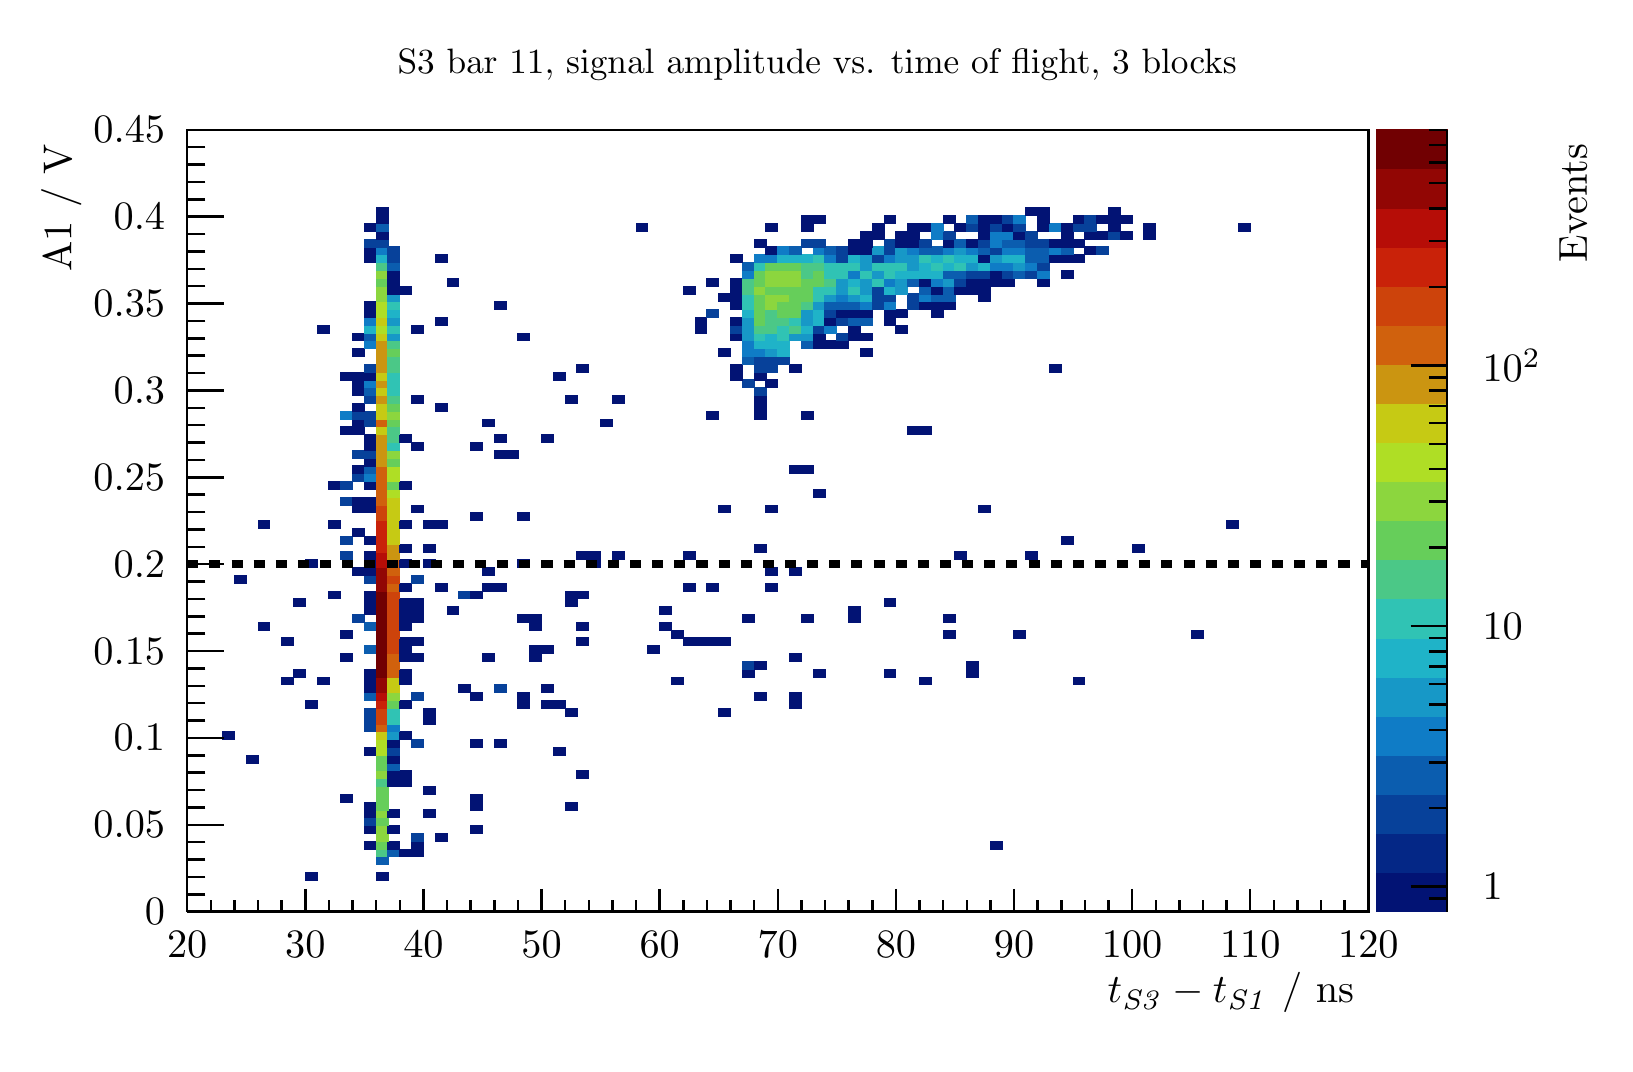
\begin{tikzpicture}
\pgfdeclareplotmark{cross} {
\pgfpathmoveto{\pgfpoint{-0.3\pgfplotmarksize}{\pgfplotmarksize}}
\pgfpathlineto{\pgfpoint{+0.3\pgfplotmarksize}{\pgfplotmarksize}}
\pgfpathlineto{\pgfpoint{+0.3\pgfplotmarksize}{0.3\pgfplotmarksize}}
\pgfpathlineto{\pgfpoint{+1\pgfplotmarksize}{0.3\pgfplotmarksize}}
\pgfpathlineto{\pgfpoint{+1\pgfplotmarksize}{-0.3\pgfplotmarksize}}
\pgfpathlineto{\pgfpoint{+0.3\pgfplotmarksize}{-0.3\pgfplotmarksize}}
\pgfpathlineto{\pgfpoint{+0.3\pgfplotmarksize}{-1.\pgfplotmarksize}}
\pgfpathlineto{\pgfpoint{-0.3\pgfplotmarksize}{-1.\pgfplotmarksize}}
\pgfpathlineto{\pgfpoint{-0.3\pgfplotmarksize}{-0.3\pgfplotmarksize}}
\pgfpathlineto{\pgfpoint{-1.\pgfplotmarksize}{-0.3\pgfplotmarksize}}
\pgfpathlineto{\pgfpoint{-1.\pgfplotmarksize}{0.3\pgfplotmarksize}}
\pgfpathlineto{\pgfpoint{-0.3\pgfplotmarksize}{0.3\pgfplotmarksize}}
\pgfpathclose
\pgfusepathqstroke
}
\pgfdeclareplotmark{cross*} {
\pgfpathmoveto{\pgfpoint{-0.3\pgfplotmarksize}{\pgfplotmarksize}}
\pgfpathlineto{\pgfpoint{+0.3\pgfplotmarksize}{\pgfplotmarksize}}
\pgfpathlineto{\pgfpoint{+0.3\pgfplotmarksize}{0.3\pgfplotmarksize}}
\pgfpathlineto{\pgfpoint{+1\pgfplotmarksize}{0.3\pgfplotmarksize}}
\pgfpathlineto{\pgfpoint{+1\pgfplotmarksize}{-0.3\pgfplotmarksize}}
\pgfpathlineto{\pgfpoint{+0.3\pgfplotmarksize}{-0.3\pgfplotmarksize}}
\pgfpathlineto{\pgfpoint{+0.3\pgfplotmarksize}{-1.\pgfplotmarksize}}
\pgfpathlineto{\pgfpoint{-0.3\pgfplotmarksize}{-1.\pgfplotmarksize}}
\pgfpathlineto{\pgfpoint{-0.3\pgfplotmarksize}{-0.3\pgfplotmarksize}}
\pgfpathlineto{\pgfpoint{-1.\pgfplotmarksize}{-0.3\pgfplotmarksize}}
\pgfpathlineto{\pgfpoint{-1.\pgfplotmarksize}{0.3\pgfplotmarksize}}
\pgfpathlineto{\pgfpoint{-0.3\pgfplotmarksize}{0.3\pgfplotmarksize}}
\pgfpathclose
\pgfusepathqfillstroke
}
\pgfdeclareplotmark{newstar} {
\pgfpathmoveto{\pgfqpoint{0pt}{\pgfplotmarksize}}
\pgfpathlineto{\pgfqpointpolar{44}{0.5\pgfplotmarksize}}
\pgfpathlineto{\pgfqpointpolar{18}{\pgfplotmarksize}}
\pgfpathlineto{\pgfqpointpolar{-20}{0.5\pgfplotmarksize}}
\pgfpathlineto{\pgfqpointpolar{-54}{\pgfplotmarksize}}
\pgfpathlineto{\pgfqpointpolar{-90}{0.5\pgfplotmarksize}}
\pgfpathlineto{\pgfqpointpolar{234}{\pgfplotmarksize}}
\pgfpathlineto{\pgfqpointpolar{198}{0.5\pgfplotmarksize}}
\pgfpathlineto{\pgfqpointpolar{162}{\pgfplotmarksize}}
\pgfpathlineto{\pgfqpointpolar{134}{0.5\pgfplotmarksize}}
\pgfpathclose
\pgfusepathqstroke
}
\pgfdeclareplotmark{newstar*} {
\pgfpathmoveto{\pgfqpoint{0pt}{\pgfplotmarksize}}
\pgfpathlineto{\pgfqpointpolar{44}{0.5\pgfplotmarksize}}
\pgfpathlineto{\pgfqpointpolar{18}{\pgfplotmarksize}}
\pgfpathlineto{\pgfqpointpolar{-20}{0.5\pgfplotmarksize}}
\pgfpathlineto{\pgfqpointpolar{-54}{\pgfplotmarksize}}
\pgfpathlineto{\pgfqpointpolar{-90}{0.5\pgfplotmarksize}}
\pgfpathlineto{\pgfqpointpolar{234}{\pgfplotmarksize}}
\pgfpathlineto{\pgfqpointpolar{198}{0.5\pgfplotmarksize}}
\pgfpathlineto{\pgfqpointpolar{162}{\pgfplotmarksize}}
\pgfpathlineto{\pgfqpointpolar{134}{0.5\pgfplotmarksize}}
\pgfpathclose
\pgfusepathqfillstroke
}
\definecolor{c}{rgb}{1,1,1};
\draw [color=c, fill=c] (0,0) rectangle (20,12.8962);
\draw [color=c, fill=c] (2,1.6765) rectangle (17,11.6066);
\definecolor{c}{rgb}{0,0,0};
\draw [c,line width=0.9] (2,1.6765) -- (2,11.6066) -- (17,11.6066) -- (17,1.6765) -- (2,1.6765);
\definecolor{c}{rgb}{1,1,1};
\draw [color=c, fill=c] (2,1.6765) rectangle (17,11.6066);
\definecolor{c}{rgb}{0,0,0};
\draw [c,line width=0.9] (2,1.6765) -- (2,11.6066) -- (17,11.6066) -- (17,1.6765) -- (2,1.6765);
\definecolor{c}{rgb}{0.00759013,0.0728653,0.45351};
\draw [color=c, fill=c] (3.5,2.0737) rectangle (3.65,2.17301);
\draw [color=c, fill=c] (4.4,2.0737) rectangle (4.55,2.17301);
\definecolor{c}{rgb}{0.0428922,0.365196,0.687255};
\draw [color=c, fill=c] (4.4,2.27231) rectangle (4.55,2.37161);
\definecolor{c}{rgb}{0.29326,0.785539,0.529779};
\draw [color=c, fill=c] (4.4,2.37161) rectangle (4.55,2.47091);
\definecolor{c}{rgb}{0.0428922,0.365196,0.687255};
\draw [color=c, fill=c] (4.55,2.37161) rectangle (4.7,2.47091);
\definecolor{c}{rgb}{0.00759013,0.0728653,0.45351};
\draw [color=c, fill=c] (4.7,2.37161) rectangle (4.85,2.47091);
\draw [color=c, fill=c] (4.85,2.37161) rectangle (5,2.47091);
\draw [color=c, fill=c] (4.25,2.47091) rectangle (4.4,2.57021);
\definecolor{c}{rgb}{0.4,0.807843,0.352941};
\draw [color=c, fill=c] (4.4,2.47091) rectangle (4.55,2.57021);
\definecolor{c}{rgb}{0.00759013,0.0728653,0.45351};
\draw [color=c, fill=c] (4.55,2.47091) rectangle (4.7,2.57021);
\draw [color=c, fill=c] (4.85,2.47091) rectangle (5,2.57021);
\draw [color=c, fill=c] (12.2,2.47091) rectangle (12.35,2.57021);
\definecolor{c}{rgb}{0.549755,0.839706,0.244608};
\draw [color=c, fill=c] (4.4,2.57021) rectangle (4.55,2.66951);
\definecolor{c}{rgb}{0.0281863,0.253431,0.604902};
\draw [color=c, fill=c] (4.85,2.57021) rectangle (5,2.66951);
\definecolor{c}{rgb}{0.00759013,0.0728653,0.45351};
\draw [color=c, fill=c] (5.15,2.57021) rectangle (5.3,2.66951);
\draw [color=c, fill=c] (4.25,2.66951) rectangle (4.4,2.76881);
\definecolor{c}{rgb}{0.549755,0.839706,0.244608};
\draw [color=c, fill=c] (4.4,2.66951) rectangle (4.55,2.76881);
\definecolor{c}{rgb}{0.00759013,0.0728653,0.45351};
\draw [color=c, fill=c] (4.55,2.66951) rectangle (4.7,2.76881);
\draw [color=c, fill=c] (5.6,2.66951) rectangle (5.75,2.76881);
\definecolor{c}{rgb}{0.0281863,0.253431,0.604902};
\draw [color=c, fill=c] (4.25,2.76881) rectangle (4.4,2.86811);
\definecolor{c}{rgb}{0.4,0.807843,0.352941};
\draw [color=c, fill=c] (4.4,2.76881) rectangle (4.55,2.86811);
\definecolor{c}{rgb}{0.00759013,0.0728653,0.45351};
\draw [color=c, fill=c] (4.25,2.86811) rectangle (4.4,2.96741);
\definecolor{c}{rgb}{0.549755,0.839706,0.244608};
\draw [color=c, fill=c] (4.4,2.86811) rectangle (4.55,2.96741);
\definecolor{c}{rgb}{0.00759013,0.0728653,0.45351};
\draw [color=c, fill=c] (4.55,2.86811) rectangle (4.7,2.96741);
\draw [color=c, fill=c] (5,2.86811) rectangle (5.15,2.96741);
\draw [color=c, fill=c] (4.25,2.96741) rectangle (4.4,3.06671);
\definecolor{c}{rgb}{0.4,0.807843,0.352941};
\draw [color=c, fill=c] (4.4,2.96741) rectangle (4.55,3.06671);
\definecolor{c}{rgb}{0.00759013,0.0728653,0.45351};
\draw [color=c, fill=c] (5.6,2.96741) rectangle (5.75,3.06671);
\draw [color=c, fill=c] (6.8,2.96741) rectangle (6.95,3.06671);
\draw [color=c, fill=c] (3.95,3.06671) rectangle (4.1,3.16601);
\definecolor{c}{rgb}{0.4,0.807843,0.352941};
\draw [color=c, fill=c] (4.4,3.06671) rectangle (4.55,3.16601);
\definecolor{c}{rgb}{0.00759013,0.0728653,0.45351};
\draw [color=c, fill=c] (5.6,3.06671) rectangle (5.75,3.16601);
\definecolor{c}{rgb}{0.4,0.807843,0.352941};
\draw [color=c, fill=c] (4.4,3.16601) rectangle (4.55,3.26531);
\definecolor{c}{rgb}{0.00759013,0.0728653,0.45351};
\draw [color=c, fill=c] (5,3.16601) rectangle (5.15,3.26531);
\definecolor{c}{rgb}{0.29326,0.785539,0.529779};
\draw [color=c, fill=c] (4.4,3.26531) rectangle (4.55,3.36461);
\definecolor{c}{rgb}{0.00759013,0.0728653,0.45351};
\draw [color=c, fill=c] (4.55,3.26531) rectangle (4.7,3.36461);
\draw [color=c, fill=c] (4.7,3.26531) rectangle (4.85,3.36461);
\definecolor{c}{rgb}{0.549755,0.839706,0.244608};
\draw [color=c, fill=c] (4.4,3.36461) rectangle (4.55,3.46391);
\definecolor{c}{rgb}{0.00759013,0.0728653,0.45351};
\draw [color=c, fill=c] (4.55,3.36461) rectangle (4.7,3.46391);
\draw [color=c, fill=c] (4.7,3.36461) rectangle (4.85,3.46391);
\draw [color=c, fill=c] (6.95,3.36461) rectangle (7.1,3.46391);
\definecolor{c}{rgb}{0.4,0.807843,0.352941};
\draw [color=c, fill=c] (4.4,3.46391) rectangle (4.55,3.56321);
\definecolor{c}{rgb}{0.0428922,0.365196,0.687255};
\draw [color=c, fill=c] (4.55,3.46391) rectangle (4.7,3.56321);
\definecolor{c}{rgb}{0.00759013,0.0728653,0.45351};
\draw [color=c, fill=c] (2.75,3.56321) rectangle (2.9,3.66251);
\definecolor{c}{rgb}{0.4,0.807843,0.352941};
\draw [color=c, fill=c] (4.4,3.56321) rectangle (4.55,3.66251);
\definecolor{c}{rgb}{0.00759013,0.0728653,0.45351};
\draw [color=c, fill=c] (4.55,3.56321) rectangle (4.7,3.66251);
\draw [color=c, fill=c] (4.25,3.66251) rectangle (4.4,3.76181);
\definecolor{c}{rgb}{0.68799,0.869118,0.144608};
\draw [color=c, fill=c] (4.4,3.66251) rectangle (4.55,3.76181);
\definecolor{c}{rgb}{0.0281863,0.253431,0.604902};
\draw [color=c, fill=c] (4.55,3.66251) rectangle (4.7,3.76181);
\definecolor{c}{rgb}{0.00759013,0.0728653,0.45351};
\draw [color=c, fill=c] (6.65,3.66251) rectangle (6.8,3.76181);
\definecolor{c}{rgb}{0.68799,0.869118,0.144608};
\draw [color=c, fill=c] (4.4,3.76181) rectangle (4.55,3.86111);
\definecolor{c}{rgb}{0.00759013,0.0728653,0.45351};
\draw [color=c, fill=c] (4.55,3.76181) rectangle (4.7,3.86111);
\definecolor{c}{rgb}{0.0281863,0.253431,0.604902};
\draw [color=c, fill=c] (4.85,3.76181) rectangle (5,3.86111);
\definecolor{c}{rgb}{0.00759013,0.0728653,0.45351};
\draw [color=c, fill=c] (5.6,3.76181) rectangle (5.75,3.86111);
\draw [color=c, fill=c] (5.9,3.76181) rectangle (6.05,3.86111);
\draw [color=c, fill=c] (2.45,3.86111) rectangle (2.6,3.96042);
\definecolor{c}{rgb}{0.777451,0.791422,0.0796569};
\draw [color=c, fill=c] (4.4,3.86111) rectangle (4.55,3.96042);
\definecolor{c}{rgb}{0.0906863,0.594608,0.78125};
\draw [color=c, fill=c] (4.55,3.86111) rectangle (4.7,3.96042);
\definecolor{c}{rgb}{0.00759013,0.0728653,0.45351};
\draw [color=c, fill=c] (4.7,3.86111) rectangle (4.85,3.96042);
\definecolor{c}{rgb}{0.0281863,0.253431,0.604902};
\draw [color=c, fill=c] (4.25,3.96042) rectangle (4.4,4.05972);
\definecolor{c}{rgb}{0.815686,0.380392,0.0509804};
\draw [color=c, fill=c] (4.4,3.96042) rectangle (4.55,4.05972);
\definecolor{c}{rgb}{0.0588235,0.486275,0.776471};
\draw [color=c, fill=c] (4.55,3.96042) rectangle (4.7,4.05972);
\definecolor{c}{rgb}{0.0281863,0.253431,0.604902};
\draw [color=c, fill=c] (4.25,4.05972) rectangle (4.4,4.15902);
\definecolor{c}{rgb}{0.802451,0.261275,0.0436275};
\draw [color=c, fill=c] (4.4,4.05972) rectangle (4.55,4.15902);
\definecolor{c}{rgb}{0.18652,0.763235,0.706618};
\draw [color=c, fill=c] (4.55,4.05972) rectangle (4.7,4.15902);
\definecolor{c}{rgb}{0.00759013,0.0728653,0.45351};
\draw [color=c, fill=c] (5,4.05972) rectangle (5.15,4.15902);
\definecolor{c}{rgb}{0.0281863,0.253431,0.604902};
\draw [color=c, fill=c] (4.25,4.15902) rectangle (4.4,4.25832);
\definecolor{c}{rgb}{0.802451,0.261275,0.0436275};
\draw [color=c, fill=c] (4.4,4.15902) rectangle (4.55,4.25832);
\definecolor{c}{rgb}{0.18652,0.763235,0.706618};
\draw [color=c, fill=c] (4.55,4.15902) rectangle (4.7,4.25832);
\definecolor{c}{rgb}{0.00759013,0.0728653,0.45351};
\draw [color=c, fill=c] (5,4.15902) rectangle (5.15,4.25832);
\draw [color=c, fill=c] (6.8,4.15902) rectangle (6.95,4.25832);
\draw [color=c, fill=c] (8.75,4.15902) rectangle (8.9,4.25832);
\draw [color=c, fill=c] (3.5,4.25832) rectangle (3.65,4.35762);
\definecolor{c}{rgb}{0.788113,0.13223,0.0356618};
\draw [color=c, fill=c] (4.4,4.25832) rectangle (4.55,4.35762);
\definecolor{c}{rgb}{0.4,0.807843,0.352941};
\draw [color=c, fill=c] (4.55,4.25832) rectangle (4.7,4.35762);
\definecolor{c}{rgb}{0.00759013,0.0728653,0.45351};
\draw [color=c, fill=c] (4.7,4.25832) rectangle (4.85,4.35762);
\draw [color=c, fill=c] (6.2,4.25832) rectangle (6.35,4.35762);
\draw [color=c, fill=c] (6.5,4.25832) rectangle (6.65,4.35762);
\draw [color=c, fill=c] (6.65,4.25832) rectangle (6.8,4.35762);
\draw [color=c, fill=c] (9.65,4.25832) rectangle (9.8,4.35762);
\definecolor{c}{rgb}{0.0428922,0.365196,0.687255};
\draw [color=c, fill=c] (4.25,4.35762) rectangle (4.4,4.45692);
\definecolor{c}{rgb}{0.714951,0.0509804,0.0269608};
\draw [color=c, fill=c] (4.4,4.35762) rectangle (4.55,4.45692);
\definecolor{c}{rgb}{0.549755,0.839706,0.244608};
\draw [color=c, fill=c] (4.55,4.35762) rectangle (4.7,4.45692);
\definecolor{c}{rgb}{0.0281863,0.253431,0.604902};
\draw [color=c, fill=c] (4.85,4.35762) rectangle (5,4.45692);
\definecolor{c}{rgb}{0.00759013,0.0728653,0.45351};
\draw [color=c, fill=c] (5.6,4.35762) rectangle (5.75,4.45692);
\draw [color=c, fill=c] (6.2,4.35762) rectangle (6.35,4.45692);
\draw [color=c, fill=c] (9.2,4.35762) rectangle (9.35,4.45692);
\draw [color=c, fill=c] (9.65,4.35762) rectangle (9.8,4.45692);
\draw [color=c, fill=c] (4.25,4.45692) rectangle (4.4,4.55622);
\definecolor{c}{rgb}{0.573162,0.0254902,0.017402};
\draw [color=c, fill=c] (4.4,4.45692) rectangle (4.55,4.55622);
\definecolor{c}{rgb}{0.777451,0.791422,0.0796569};
\draw [color=c, fill=c] (4.55,4.45692) rectangle (4.7,4.55622);
\definecolor{c}{rgb}{0.00759013,0.0728653,0.45351};
\draw [color=c, fill=c] (5.45,4.45692) rectangle (5.6,4.55622);
\definecolor{c}{rgb}{0.0281863,0.253431,0.604902};
\draw [color=c, fill=c] (5.9,4.45692) rectangle (6.05,4.55622);
\definecolor{c}{rgb}{0.00759013,0.0728653,0.45351};
\draw [color=c, fill=c] (6.5,4.45692) rectangle (6.65,4.55622);
\draw [color=c, fill=c] (3.2,4.55622) rectangle (3.35,4.65552);
\draw [color=c, fill=c] (3.65,4.55622) rectangle (3.8,4.65552);
\draw [color=c, fill=c] (4.25,4.55622) rectangle (4.4,4.65552);
\definecolor{c}{rgb}{0.573162,0.0254902,0.017402};
\draw [color=c, fill=c] (4.4,4.55622) rectangle (4.55,4.65552);
\definecolor{c}{rgb}{0.777451,0.791422,0.0796569};
\draw [color=c, fill=c] (4.55,4.55622) rectangle (4.7,4.65552);
\definecolor{c}{rgb}{0.00759013,0.0728653,0.45351};
\draw [color=c, fill=c] (4.7,4.55622) rectangle (4.85,4.65552);
\draw [color=c, fill=c] (8.15,4.55622) rectangle (8.3,4.65552);
\draw [color=c, fill=c] (11.3,4.55622) rectangle (11.45,4.65552);
\draw [color=c, fill=c] (13.25,4.55622) rectangle (13.4,4.65552);
\draw [color=c, fill=c] (3.35,4.65552) rectangle (3.5,4.75482);
\draw [color=c, fill=c] (4.25,4.65552) rectangle (4.4,4.75482);
\definecolor{c}{rgb}{0.442279,0.00196078,0.00857843};
\draw [color=c, fill=c] (4.4,4.65552) rectangle (4.55,4.75482);
\definecolor{c}{rgb}{0.815686,0.380392,0.0509804};
\draw [color=c, fill=c] (4.55,4.65552) rectangle (4.7,4.75482);
\definecolor{c}{rgb}{0.00759013,0.0728653,0.45351};
\draw [color=c, fill=c] (4.7,4.65552) rectangle (4.85,4.75482);
\draw [color=c, fill=c] (9.05,4.65552) rectangle (9.2,4.75482);
\draw [color=c, fill=c] (9.95,4.65552) rectangle (10.1,4.75482);
\draw [color=c, fill=c] (10.85,4.65552) rectangle (11,4.75482);
\draw [color=c, fill=c] (11.9,4.65552) rectangle (12.05,4.75482);
\definecolor{c}{rgb}{0.442279,0.00196078,0.00857843};
\draw [color=c, fill=c] (4.4,4.75482) rectangle (4.55,4.85412);
\definecolor{c}{rgb}{0.815686,0.380392,0.0509804};
\draw [color=c, fill=c] (4.55,4.75482) rectangle (4.7,4.85412);
\definecolor{c}{rgb}{0.0281863,0.253431,0.604902};
\draw [color=c, fill=c] (9.05,4.75482) rectangle (9.2,4.85412);
\definecolor{c}{rgb}{0.00759013,0.0728653,0.45351};
\draw [color=c, fill=c] (9.2,4.75482) rectangle (9.35,4.85412);
\draw [color=c, fill=c] (11.9,4.75482) rectangle (12.05,4.85412);
\draw [color=c, fill=c] (3.95,4.85412) rectangle (4.1,4.95342);
\definecolor{c}{rgb}{0.442279,0.00196078,0.00857843};
\draw [color=c, fill=c] (4.4,4.85412) rectangle (4.55,4.95342);
\definecolor{c}{rgb}{0.815686,0.380392,0.0509804};
\draw [color=c, fill=c] (4.55,4.85412) rectangle (4.7,4.95342);
\definecolor{c}{rgb}{0.00759013,0.0728653,0.45351};
\draw [color=c, fill=c] (4.7,4.85412) rectangle (4.85,4.95342);
\draw [color=c, fill=c] (4.85,4.85412) rectangle (5,4.95342);
\draw [color=c, fill=c] (5.75,4.85412) rectangle (5.9,4.95342);
\draw [color=c, fill=c] (6.35,4.85412) rectangle (6.5,4.95342);
\draw [color=c, fill=c] (9.65,4.85412) rectangle (9.8,4.95342);
\definecolor{c}{rgb}{0.0428922,0.365196,0.687255};
\draw [color=c, fill=c] (4.25,4.95342) rectangle (4.4,5.05272);
\definecolor{c}{rgb}{0.442279,0.00196078,0.00857843};
\draw [color=c, fill=c] (4.4,4.95342) rectangle (4.55,5.05272);
\definecolor{c}{rgb}{0.802451,0.261275,0.0436275};
\draw [color=c, fill=c] (4.55,4.95342) rectangle (4.7,5.05272);
\definecolor{c}{rgb}{0.00759013,0.0728653,0.45351};
\draw [color=c, fill=c] (4.7,4.95342) rectangle (4.85,5.05272);
\draw [color=c, fill=c] (6.35,4.95342) rectangle (6.5,5.05272);
\draw [color=c, fill=c] (6.5,4.95342) rectangle (6.65,5.05272);
\draw [color=c, fill=c] (7.85,4.95342) rectangle (8,5.05272);
\draw [color=c, fill=c] (3.2,5.05272) rectangle (3.35,5.15202);
\definecolor{c}{rgb}{0.442279,0.00196078,0.00857843};
\draw [color=c, fill=c] (4.4,5.05272) rectangle (4.55,5.15202);
\definecolor{c}{rgb}{0.802451,0.261275,0.0436275};
\draw [color=c, fill=c] (4.55,5.05272) rectangle (4.7,5.15202);
\definecolor{c}{rgb}{0.00759013,0.0728653,0.45351};
\draw [color=c, fill=c] (4.7,5.05272) rectangle (4.85,5.15202);
\draw [color=c, fill=c] (4.85,5.05272) rectangle (5,5.15202);
\draw [color=c, fill=c] (6.95,5.05272) rectangle (7.1,5.15202);
\draw [color=c, fill=c] (8.3,5.05272) rectangle (8.45,5.15202);
\draw [color=c, fill=c] (8.45,5.05272) rectangle (8.6,5.15202);
\draw [color=c, fill=c] (8.6,5.05272) rectangle (8.75,5.15202);
\draw [color=c, fill=c] (8.75,5.05272) rectangle (8.9,5.15202);
\draw [color=c, fill=c] (3.95,5.15202) rectangle (4.1,5.25132);
\definecolor{c}{rgb}{0.442279,0.00196078,0.00857843};
\draw [color=c, fill=c] (4.4,5.15202) rectangle (4.55,5.25132);
\definecolor{c}{rgb}{0.802451,0.261275,0.0436275};
\draw [color=c, fill=c] (4.55,5.15202) rectangle (4.7,5.25132);
\definecolor{c}{rgb}{0.00759013,0.0728653,0.45351};
\draw [color=c, fill=c] (8.15,5.15202) rectangle (8.3,5.25132);
\draw [color=c, fill=c] (11.6,5.15202) rectangle (11.75,5.25132);
\draw [color=c, fill=c] (12.5,5.15202) rectangle (12.65,5.25132);
\draw [color=c, fill=c] (14.75,5.15202) rectangle (14.9,5.25132);
\draw [color=c, fill=c] (2.9,5.25132) rectangle (3.05,5.35062);
\definecolor{c}{rgb}{0.0428922,0.365196,0.687255};
\draw [color=c, fill=c] (4.25,5.25132) rectangle (4.4,5.35062);
\definecolor{c}{rgb}{0.442279,0.00196078,0.00857843};
\draw [color=c, fill=c] (4.4,5.25132) rectangle (4.55,5.35062);
\definecolor{c}{rgb}{0.802451,0.261275,0.0436275};
\draw [color=c, fill=c] (4.55,5.25132) rectangle (4.7,5.35062);
\definecolor{c}{rgb}{0.00759013,0.0728653,0.45351};
\draw [color=c, fill=c] (4.7,5.25132) rectangle (4.85,5.35062);
\draw [color=c, fill=c] (6.35,5.25132) rectangle (6.5,5.35062);
\draw [color=c, fill=c] (6.95,5.25132) rectangle (7.1,5.35062);
\draw [color=c, fill=c] (8,5.25132) rectangle (8.15,5.35062);
\definecolor{c}{rgb}{0.0281863,0.253431,0.604902};
\draw [color=c, fill=c] (4.1,5.35062) rectangle (4.25,5.44992);
\definecolor{c}{rgb}{0.442279,0.00196078,0.00857843};
\draw [color=c, fill=c] (4.4,5.35062) rectangle (4.55,5.44992);
\definecolor{c}{rgb}{0.802451,0.261275,0.0436275};
\draw [color=c, fill=c] (4.55,5.35062) rectangle (4.7,5.44992);
\definecolor{c}{rgb}{0.00759013,0.0728653,0.45351};
\draw [color=c, fill=c] (4.7,5.35062) rectangle (4.85,5.44992);
\draw [color=c, fill=c] (4.85,5.35062) rectangle (5,5.44992);
\draw [color=c, fill=c] (6.2,5.35062) rectangle (6.35,5.44992);
\draw [color=c, fill=c] (6.35,5.35062) rectangle (6.5,5.44992);
\draw [color=c, fill=c] (9.05,5.35062) rectangle (9.2,5.44992);
\draw [color=c, fill=c] (9.8,5.35062) rectangle (9.95,5.44992);
\draw [color=c, fill=c] (10.4,5.35062) rectangle (10.55,5.44992);
\draw [color=c, fill=c] (11.6,5.35062) rectangle (11.75,5.44992);
\draw [color=c, fill=c] (4.25,5.44992) rectangle (4.4,5.54922);
\definecolor{c}{rgb}{0.442279,0.00196078,0.00857843};
\draw [color=c, fill=c] (4.4,5.44992) rectangle (4.55,5.54922);
\definecolor{c}{rgb}{0.802451,0.261275,0.0436275};
\draw [color=c, fill=c] (4.55,5.44992) rectangle (4.7,5.54922);
\definecolor{c}{rgb}{0.00759013,0.0728653,0.45351};
\draw [color=c, fill=c] (4.7,5.44992) rectangle (4.85,5.54922);
\draw [color=c, fill=c] (4.85,5.44992) rectangle (5,5.54922);
\draw [color=c, fill=c] (5.3,5.44992) rectangle (5.45,5.54922);
\draw [color=c, fill=c] (8,5.44992) rectangle (8.15,5.54922);
\draw [color=c, fill=c] (10.4,5.44992) rectangle (10.55,5.54922);
\draw [color=c, fill=c] (3.35,5.54922) rectangle (3.5,5.64852);
\draw [color=c, fill=c] (4.25,5.54922) rectangle (4.4,5.64852);
\definecolor{c}{rgb}{0.442279,0.00196078,0.00857843};
\draw [color=c, fill=c] (4.4,5.54922) rectangle (4.55,5.64852);
\definecolor{c}{rgb}{0.802451,0.261275,0.0436275};
\draw [color=c, fill=c] (4.55,5.54922) rectangle (4.7,5.64852);
\definecolor{c}{rgb}{0.00759013,0.0728653,0.45351};
\draw [color=c, fill=c] (4.7,5.54922) rectangle (4.85,5.64852);
\draw [color=c, fill=c] (4.85,5.54922) rectangle (5,5.64852);
\draw [color=c, fill=c] (6.8,5.54922) rectangle (6.95,5.64852);
\draw [color=c, fill=c] (10.85,5.54922) rectangle (11,5.64852);
\draw [color=c, fill=c] (3.8,5.64852) rectangle (3.95,5.74783);
\draw [color=c, fill=c] (4.25,5.64852) rectangle (4.4,5.74783);
\definecolor{c}{rgb}{0.442279,0.00196078,0.00857843};
\draw [color=c, fill=c] (4.4,5.64852) rectangle (4.55,5.74783);
\definecolor{c}{rgb}{0.802451,0.261275,0.0436275};
\draw [color=c, fill=c] (4.55,5.64852) rectangle (4.7,5.74783);
\definecolor{c}{rgb}{0.0281863,0.253431,0.604902};
\draw [color=c, fill=c] (5.45,5.64852) rectangle (5.6,5.74783);
\definecolor{c}{rgb}{0.00759013,0.0728653,0.45351};
\draw [color=c, fill=c] (5.6,5.64852) rectangle (5.75,5.74783);
\draw [color=c, fill=c] (6.8,5.64852) rectangle (6.95,5.74783);
\draw [color=c, fill=c] (6.95,5.64852) rectangle (7.1,5.74783);
\definecolor{c}{rgb}{0.573162,0.0254902,0.017402};
\draw [color=c, fill=c] (4.4,5.74783) rectangle (4.55,5.84713);
\definecolor{c}{rgb}{0.815686,0.380392,0.0509804};
\draw [color=c, fill=c] (4.55,5.74783) rectangle (4.7,5.84713);
\definecolor{c}{rgb}{0.00759013,0.0728653,0.45351};
\draw [color=c, fill=c] (4.7,5.74783) rectangle (4.85,5.84713);
\draw [color=c, fill=c] (5.15,5.74783) rectangle (5.3,5.84713);
\draw [color=c, fill=c] (5.75,5.74783) rectangle (5.9,5.84713);
\draw [color=c, fill=c] (5.9,5.74783) rectangle (6.05,5.84713);
\draw [color=c, fill=c] (8.3,5.74783) rectangle (8.45,5.84713);
\draw [color=c, fill=c] (8.6,5.74783) rectangle (8.75,5.84713);
\draw [color=c, fill=c] (9.35,5.74783) rectangle (9.5,5.84713);
\draw [color=c, fill=c] (2.6,5.84713) rectangle (2.75,5.94643);
\definecolor{c}{rgb}{0.0281863,0.253431,0.604902};
\draw [color=c, fill=c] (4.25,5.84713) rectangle (4.4,5.94643);
\definecolor{c}{rgb}{0.573162,0.0254902,0.017402};
\draw [color=c, fill=c] (4.4,5.84713) rectangle (4.55,5.94643);
\definecolor{c}{rgb}{0.802451,0.261275,0.0436275};
\draw [color=c, fill=c] (4.55,5.84713) rectangle (4.7,5.94643);
\definecolor{c}{rgb}{0.0281863,0.253431,0.604902};
\draw [color=c, fill=c] (4.85,5.84713) rectangle (5,5.94643);
\definecolor{c}{rgb}{0.00759013,0.0728653,0.45351};
\draw [color=c, fill=c] (4.1,5.94643) rectangle (4.25,6.04573);
\draw [color=c, fill=c] (4.25,5.94643) rectangle (4.4,6.04573);
\definecolor{c}{rgb}{0.573162,0.0254902,0.017402};
\draw [color=c, fill=c] (4.4,5.94643) rectangle (4.55,6.04573);
\definecolor{c}{rgb}{0.815686,0.380392,0.0509804};
\draw [color=c, fill=c] (4.55,5.94643) rectangle (4.7,6.04573);
\definecolor{c}{rgb}{0.00759013,0.0728653,0.45351};
\draw [color=c, fill=c] (5.75,5.94643) rectangle (5.9,6.04573);
\draw [color=c, fill=c] (9.35,5.94643) rectangle (9.5,6.04573);
\draw [color=c, fill=c] (9.65,5.94643) rectangle (9.8,6.04573);
\draw [color=c, fill=c] (3.5,6.04573) rectangle (3.65,6.14503);
\draw [color=c, fill=c] (4.25,6.04573) rectangle (4.4,6.14503);
\definecolor{c}{rgb}{0.714951,0.0509804,0.0269608};
\draw [color=c, fill=c] (4.4,6.04573) rectangle (4.55,6.14503);
\definecolor{c}{rgb}{0.815686,0.380392,0.0509804};
\draw [color=c, fill=c] (4.55,6.04573) rectangle (4.7,6.14503);
\definecolor{c}{rgb}{0.00759013,0.0728653,0.45351};
\draw [color=c, fill=c] (4.7,6.04573) rectangle (4.85,6.14503);
\draw [color=c, fill=c] (5,6.04573) rectangle (5.15,6.14503);
\draw [color=c, fill=c] (6.2,6.04573) rectangle (6.35,6.14503);
\draw [color=c, fill=c] (7.1,6.04573) rectangle (7.25,6.14503);
\definecolor{c}{rgb}{0.0281863,0.253431,0.604902};
\draw [color=c, fill=c] (3.95,6.14503) rectangle (4.1,6.24433);
\definecolor{c}{rgb}{0.00759013,0.0728653,0.45351};
\draw [color=c, fill=c] (4.25,6.14503) rectangle (4.4,6.24433);
\definecolor{c}{rgb}{0.714951,0.0509804,0.0269608};
\draw [color=c, fill=c] (4.4,6.14503) rectangle (4.55,6.24433);
\definecolor{c}{rgb}{0.796569,0.585907,0.0653186};
\draw [color=c, fill=c] (4.55,6.14503) rectangle (4.7,6.24433);
\definecolor{c}{rgb}{0.00759013,0.0728653,0.45351};
\draw [color=c, fill=c] (6.95,6.14503) rectangle (7.1,6.24433);
\draw [color=c, fill=c] (7.1,6.14503) rectangle (7.25,6.24433);
\draw [color=c, fill=c] (7.4,6.14503) rectangle (7.55,6.24433);
\draw [color=c, fill=c] (8.3,6.14503) rectangle (8.45,6.24433);
\draw [color=c, fill=c] (11.75,6.14503) rectangle (11.9,6.24433);
\draw [color=c, fill=c] (12.65,6.14503) rectangle (12.8,6.24433);
\definecolor{c}{rgb}{0.788113,0.13223,0.0356618};
\draw [color=c, fill=c] (4.4,6.24433) rectangle (4.55,6.34363);
\definecolor{c}{rgb}{0.796569,0.585907,0.0653186};
\draw [color=c, fill=c] (4.55,6.24433) rectangle (4.7,6.34363);
\definecolor{c}{rgb}{0.00759013,0.0728653,0.45351};
\draw [color=c, fill=c] (4.7,6.24433) rectangle (4.85,6.34363);
\draw [color=c, fill=c] (5,6.24433) rectangle (5.15,6.34363);
\draw [color=c, fill=c] (9.2,6.24433) rectangle (9.35,6.34363);
\draw [color=c, fill=c] (14,6.24433) rectangle (14.15,6.34363);
\definecolor{c}{rgb}{0.0281863,0.253431,0.604902};
\draw [color=c, fill=c] (3.95,6.34363) rectangle (4.1,6.44293);
\definecolor{c}{rgb}{0.00759013,0.0728653,0.45351};
\draw [color=c, fill=c] (4.25,6.34363) rectangle (4.4,6.44293);
\definecolor{c}{rgb}{0.788113,0.13223,0.0356618};
\draw [color=c, fill=c] (4.4,6.34363) rectangle (4.55,6.44293);
\definecolor{c}{rgb}{0.777451,0.791422,0.0796569};
\draw [color=c, fill=c] (4.55,6.34363) rectangle (4.7,6.44293);
\definecolor{c}{rgb}{0.00759013,0.0728653,0.45351};
\draw [color=c, fill=c] (13.1,6.34363) rectangle (13.25,6.44293);
\draw [color=c, fill=c] (4.1,6.44293) rectangle (4.25,6.54223);
\definecolor{c}{rgb}{0.788113,0.13223,0.0356618};
\draw [color=c, fill=c] (4.4,6.44293) rectangle (4.55,6.54223);
\definecolor{c}{rgb}{0.777451,0.791422,0.0796569};
\draw [color=c, fill=c] (4.55,6.44293) rectangle (4.7,6.54223);
\definecolor{c}{rgb}{0.00759013,0.0728653,0.45351};
\draw [color=c, fill=c] (2.9,6.54223) rectangle (3.05,6.64153);
\draw [color=c, fill=c] (3.8,6.54223) rectangle (3.95,6.64153);
\definecolor{c}{rgb}{0.788113,0.13223,0.0356618};
\draw [color=c, fill=c] (4.4,6.54223) rectangle (4.55,6.64153);
\definecolor{c}{rgb}{0.777451,0.791422,0.0796569};
\draw [color=c, fill=c] (4.55,6.54223) rectangle (4.7,6.64153);
\definecolor{c}{rgb}{0.00759013,0.0728653,0.45351};
\draw [color=c, fill=c] (4.7,6.54223) rectangle (4.85,6.64153);
\draw [color=c, fill=c] (5,6.54223) rectangle (5.15,6.64153);
\draw [color=c, fill=c] (5.15,6.54223) rectangle (5.3,6.64153);
\draw [color=c, fill=c] (15.2,6.54223) rectangle (15.35,6.64153);
\definecolor{c}{rgb}{0.802451,0.261275,0.0436275};
\draw [color=c, fill=c] (4.4,6.64153) rectangle (4.55,6.74083);
\definecolor{c}{rgb}{0.777451,0.791422,0.0796569};
\draw [color=c, fill=c] (4.55,6.64153) rectangle (4.7,6.74083);
\definecolor{c}{rgb}{0.00759013,0.0728653,0.45351};
\draw [color=c, fill=c] (5.6,6.64153) rectangle (5.75,6.74083);
\draw [color=c, fill=c] (6.2,6.64153) rectangle (6.35,6.74083);
\draw [color=c, fill=c] (4.1,6.74083) rectangle (4.25,6.84013);
\draw [color=c, fill=c] (4.25,6.74083) rectangle (4.4,6.84013);
\definecolor{c}{rgb}{0.802451,0.261275,0.0436275};
\draw [color=c, fill=c] (4.4,6.74083) rectangle (4.55,6.84013);
\definecolor{c}{rgb}{0.777451,0.791422,0.0796569};
\draw [color=c, fill=c] (4.55,6.74083) rectangle (4.7,6.84013);
\definecolor{c}{rgb}{0.00759013,0.0728653,0.45351};
\draw [color=c, fill=c] (4.85,6.74083) rectangle (5,6.84013);
\draw [color=c, fill=c] (8.75,6.74083) rectangle (8.9,6.84013);
\draw [color=c, fill=c] (9.35,6.74083) rectangle (9.5,6.84013);
\draw [color=c, fill=c] (12.05,6.74083) rectangle (12.2,6.84013);
\definecolor{c}{rgb}{0.0281863,0.253431,0.604902};
\draw [color=c, fill=c] (3.95,6.84013) rectangle (4.1,6.93943);
\definecolor{c}{rgb}{0.00759013,0.0728653,0.45351};
\draw [color=c, fill=c] (4.1,6.84013) rectangle (4.25,6.93943);
\draw [color=c, fill=c] (4.25,6.84013) rectangle (4.4,6.93943);
\definecolor{c}{rgb}{0.815686,0.380392,0.0509804};
\draw [color=c, fill=c] (4.4,6.84013) rectangle (4.55,6.93943);
\definecolor{c}{rgb}{0.777451,0.791422,0.0796569};
\draw [color=c, fill=c] (4.55,6.84013) rectangle (4.7,6.93943);
\definecolor{c}{rgb}{0.815686,0.380392,0.0509804};
\draw [color=c, fill=c] (4.4,6.93943) rectangle (4.55,7.03873);
\definecolor{c}{rgb}{0.68799,0.869118,0.144608};
\draw [color=c, fill=c] (4.55,6.93943) rectangle (4.7,7.03873);
\definecolor{c}{rgb}{0.00759013,0.0728653,0.45351};
\draw [color=c, fill=c] (9.95,6.93943) rectangle (10.1,7.03873);
\draw [color=c, fill=c] (3.8,7.03873) rectangle (3.95,7.13803);
\definecolor{c}{rgb}{0.0281863,0.253431,0.604902};
\draw [color=c, fill=c] (3.95,7.03873) rectangle (4.1,7.13803);
\definecolor{c}{rgb}{0.00759013,0.0728653,0.45351};
\draw [color=c, fill=c] (4.25,7.03873) rectangle (4.4,7.13803);
\definecolor{c}{rgb}{0.815686,0.380392,0.0509804};
\draw [color=c, fill=c] (4.4,7.03873) rectangle (4.55,7.13803);
\definecolor{c}{rgb}{0.4,0.807843,0.352941};
\draw [color=c, fill=c] (4.55,7.03873) rectangle (4.7,7.13803);
\definecolor{c}{rgb}{0.00759013,0.0728653,0.45351};
\draw [color=c, fill=c] (4.7,7.03873) rectangle (4.85,7.13803);
\definecolor{c}{rgb}{0.0281863,0.253431,0.604902};
\draw [color=c, fill=c] (4.1,7.13803) rectangle (4.25,7.23733);
\definecolor{c}{rgb}{0.0588235,0.486275,0.776471};
\draw [color=c, fill=c] (4.25,7.13803) rectangle (4.4,7.23733);
\definecolor{c}{rgb}{0.815686,0.380392,0.0509804};
\draw [color=c, fill=c] (4.4,7.13803) rectangle (4.55,7.23733);
\definecolor{c}{rgb}{0.68799,0.869118,0.144608};
\draw [color=c, fill=c] (4.55,7.13803) rectangle (4.7,7.23733);
\definecolor{c}{rgb}{0.00759013,0.0728653,0.45351};
\draw [color=c, fill=c] (4.1,7.23733) rectangle (4.25,7.33663);
\definecolor{c}{rgb}{0.0428922,0.365196,0.687255};
\draw [color=c, fill=c] (4.25,7.23733) rectangle (4.4,7.33663);
\definecolor{c}{rgb}{0.815686,0.380392,0.0509804};
\draw [color=c, fill=c] (4.4,7.23733) rectangle (4.55,7.33663);
\definecolor{c}{rgb}{0.68799,0.869118,0.144608};
\draw [color=c, fill=c] (4.55,7.23733) rectangle (4.7,7.33663);
\definecolor{c}{rgb}{0.00759013,0.0728653,0.45351};
\draw [color=c, fill=c] (9.65,7.23733) rectangle (9.8,7.33663);
\draw [color=c, fill=c] (9.8,7.23733) rectangle (9.95,7.33663);
\draw [color=c, fill=c] (4.25,7.33663) rectangle (4.4,7.43593);
\definecolor{c}{rgb}{0.796569,0.585907,0.0653186};
\draw [color=c, fill=c] (4.4,7.33663) rectangle (4.55,7.43593);
\definecolor{c}{rgb}{0.4,0.807843,0.352941};
\draw [color=c, fill=c] (4.55,7.33663) rectangle (4.7,7.43593);
\definecolor{c}{rgb}{0.0281863,0.253431,0.604902};
\draw [color=c, fill=c] (4.1,7.43593) rectangle (4.25,7.53523);
\draw [color=c, fill=c] (4.25,7.43593) rectangle (4.4,7.53523);
\definecolor{c}{rgb}{0.796569,0.585907,0.0653186};
\draw [color=c, fill=c] (4.4,7.43593) rectangle (4.55,7.53523);
\definecolor{c}{rgb}{0.549755,0.839706,0.244608};
\draw [color=c, fill=c] (4.55,7.43593) rectangle (4.7,7.53523);
\definecolor{c}{rgb}{0.00759013,0.0728653,0.45351};
\draw [color=c, fill=c] (5.9,7.43593) rectangle (6.05,7.53523);
\draw [color=c, fill=c] (6.05,7.43593) rectangle (6.2,7.53523);
\draw [color=c, fill=c] (4.25,7.53523) rectangle (4.4,7.63454);
\definecolor{c}{rgb}{0.796569,0.585907,0.0653186};
\draw [color=c, fill=c] (4.4,7.53523) rectangle (4.55,7.63454);
\definecolor{c}{rgb}{0.18652,0.763235,0.706618};
\draw [color=c, fill=c] (4.55,7.53523) rectangle (4.7,7.63454);
\definecolor{c}{rgb}{0.00759013,0.0728653,0.45351};
\draw [color=c, fill=c] (4.85,7.53523) rectangle (5,7.63454);
\draw [color=c, fill=c] (5.6,7.53523) rectangle (5.75,7.63454);
\draw [color=c, fill=c] (4.25,7.63454) rectangle (4.4,7.73384);
\definecolor{c}{rgb}{0.796569,0.585907,0.0653186};
\draw [color=c, fill=c] (4.4,7.63454) rectangle (4.55,7.73384);
\definecolor{c}{rgb}{0.29326,0.785539,0.529779};
\draw [color=c, fill=c] (4.55,7.63454) rectangle (4.7,7.73384);
\definecolor{c}{rgb}{0.00759013,0.0728653,0.45351};
\draw [color=c, fill=c] (4.7,7.63454) rectangle (4.85,7.73384);
\draw [color=c, fill=c] (5.9,7.63454) rectangle (6.05,7.73384);
\draw [color=c, fill=c] (6.5,7.63454) rectangle (6.65,7.73384);
\draw [color=c, fill=c] (3.95,7.73384) rectangle (4.1,7.83314);
\draw [color=c, fill=c] (4.1,7.73384) rectangle (4.25,7.83314);
\definecolor{c}{rgb}{0.777451,0.791422,0.0796569};
\draw [color=c, fill=c] (4.4,7.73384) rectangle (4.55,7.83314);
\definecolor{c}{rgb}{0.29326,0.785539,0.529779};
\draw [color=c, fill=c] (4.55,7.73384) rectangle (4.7,7.83314);
\definecolor{c}{rgb}{0.00759013,0.0728653,0.45351};
\draw [color=c, fill=c] (11.15,7.73384) rectangle (11.3,7.83314);
\draw [color=c, fill=c] (11.3,7.73384) rectangle (11.45,7.83314);
\draw [color=c, fill=c] (4.1,7.83314) rectangle (4.25,7.93244);
\definecolor{c}{rgb}{0.0281863,0.253431,0.604902};
\draw [color=c, fill=c] (4.25,7.83314) rectangle (4.4,7.93244);
\definecolor{c}{rgb}{0.815686,0.380392,0.0509804};
\draw [color=c, fill=c] (4.4,7.83314) rectangle (4.55,7.93244);
\definecolor{c}{rgb}{0.4,0.807843,0.352941};
\draw [color=c, fill=c] (4.55,7.83314) rectangle (4.7,7.93244);
\definecolor{c}{rgb}{0.00759013,0.0728653,0.45351};
\draw [color=c, fill=c] (5.75,7.83314) rectangle (5.9,7.93244);
\draw [color=c, fill=c] (7.25,7.83314) rectangle (7.4,7.93244);
\definecolor{c}{rgb}{0.0588235,0.486275,0.776471};
\draw [color=c, fill=c] (3.95,7.93244) rectangle (4.1,8.03174);
\definecolor{c}{rgb}{0.0281863,0.253431,0.604902};
\draw [color=c, fill=c] (4.1,7.93244) rectangle (4.25,8.03174);
\draw [color=c, fill=c] (4.25,7.93244) rectangle (4.4,8.03174);
\definecolor{c}{rgb}{0.777451,0.791422,0.0796569};
\draw [color=c, fill=c] (4.4,7.93244) rectangle (4.55,8.03174);
\definecolor{c}{rgb}{0.549755,0.839706,0.244608};
\draw [color=c, fill=c] (4.55,7.93244) rectangle (4.7,8.03174);
\definecolor{c}{rgb}{0.00759013,0.0728653,0.45351};
\draw [color=c, fill=c] (8.6,7.93244) rectangle (8.75,8.03174);
\draw [color=c, fill=c] (9.2,7.93244) rectangle (9.35,8.03174);
\draw [color=c, fill=c] (9.8,7.93244) rectangle (9.95,8.03174);
\draw [color=c, fill=c] (4.1,8.03174) rectangle (4.25,8.13104);
\definecolor{c}{rgb}{0.777451,0.791422,0.0796569};
\draw [color=c, fill=c] (4.4,8.03174) rectangle (4.55,8.13104);
\definecolor{c}{rgb}{0.4,0.807843,0.352941};
\draw [color=c, fill=c] (4.55,8.03174) rectangle (4.7,8.13104);
\definecolor{c}{rgb}{0.00759013,0.0728653,0.45351};
\draw [color=c, fill=c] (5.15,8.03174) rectangle (5.3,8.13104);
\draw [color=c, fill=c] (9.2,8.03174) rectangle (9.35,8.13104);
\definecolor{c}{rgb}{0.0281863,0.253431,0.604902};
\draw [color=c, fill=c] (4.25,8.13104) rectangle (4.4,8.23034);
\definecolor{c}{rgb}{0.796569,0.585907,0.0653186};
\draw [color=c, fill=c] (4.4,8.13104) rectangle (4.55,8.23034);
\definecolor{c}{rgb}{0.29326,0.785539,0.529779};
\draw [color=c, fill=c] (4.55,8.13104) rectangle (4.7,8.23034);
\definecolor{c}{rgb}{0.00759013,0.0728653,0.45351};
\draw [color=c, fill=c] (4.85,8.13104) rectangle (5,8.23034);
\draw [color=c, fill=c] (6.8,8.13104) rectangle (6.95,8.23034);
\draw [color=c, fill=c] (7.4,8.13104) rectangle (7.55,8.23034);
\draw [color=c, fill=c] (9.2,8.13104) rectangle (9.35,8.23034);
\draw [color=c, fill=c] (4.1,8.23034) rectangle (4.25,8.32964);
\definecolor{c}{rgb}{0.0428922,0.365196,0.687255};
\draw [color=c, fill=c] (4.25,8.23034) rectangle (4.4,8.32964);
\definecolor{c}{rgb}{0.777451,0.791422,0.0796569};
\draw [color=c, fill=c] (4.4,8.23034) rectangle (4.55,8.32964);
\definecolor{c}{rgb}{0.18652,0.763235,0.706618};
\draw [color=c, fill=c] (4.55,8.23034) rectangle (4.7,8.32964);
\definecolor{c}{rgb}{0.0281863,0.253431,0.604902};
\draw [color=c, fill=c] (9.2,8.23034) rectangle (9.35,8.32964);
\definecolor{c}{rgb}{0.00759013,0.0728653,0.45351};
\draw [color=c, fill=c] (4.1,8.32964) rectangle (4.25,8.42894);
\definecolor{c}{rgb}{0.0588235,0.486275,0.776471};
\draw [color=c, fill=c] (4.25,8.32964) rectangle (4.4,8.42894);
\definecolor{c}{rgb}{0.796569,0.585907,0.0653186};
\draw [color=c, fill=c] (4.4,8.32964) rectangle (4.55,8.42894);
\definecolor{c}{rgb}{0.18652,0.763235,0.706618};
\draw [color=c, fill=c] (4.55,8.32964) rectangle (4.7,8.42894);
\definecolor{c}{rgb}{0.0281863,0.253431,0.604902};
\draw [color=c, fill=c] (9.05,8.32964) rectangle (9.2,8.42894);
\definecolor{c}{rgb}{0.00759013,0.0728653,0.45351};
\draw [color=c, fill=c] (9.35,8.32964) rectangle (9.5,8.42894);
\draw [color=c, fill=c] (3.95,8.42894) rectangle (4.1,8.52824);
\draw [color=c, fill=c] (4.1,8.42894) rectangle (4.25,8.52824);
\draw [color=c, fill=c] (4.25,8.42894) rectangle (4.4,8.52824);
\definecolor{c}{rgb}{0.777451,0.791422,0.0796569};
\draw [color=c, fill=c] (4.4,8.42894) rectangle (4.55,8.52824);
\definecolor{c}{rgb}{0.18652,0.763235,0.706618};
\draw [color=c, fill=c] (4.55,8.42894) rectangle (4.7,8.52824);
\definecolor{c}{rgb}{0.00759013,0.0728653,0.45351};
\draw [color=c, fill=c] (6.65,8.42894) rectangle (6.8,8.52824);
\draw [color=c, fill=c] (8.9,8.42894) rectangle (9.05,8.52824);
\draw [color=c, fill=c] (9.2,8.42894) rectangle (9.35,8.52824);
\definecolor{c}{rgb}{0.0281863,0.253431,0.604902};
\draw [color=c, fill=c] (4.25,8.52824) rectangle (4.4,8.62754);
\definecolor{c}{rgb}{0.796569,0.585907,0.0653186};
\draw [color=c, fill=c] (4.4,8.52824) rectangle (4.55,8.62754);
\definecolor{c}{rgb}{0.29326,0.785539,0.529779};
\draw [color=c, fill=c] (4.55,8.52824) rectangle (4.7,8.62754);
\definecolor{c}{rgb}{0.00759013,0.0728653,0.45351};
\draw [color=c, fill=c] (6.95,8.52824) rectangle (7.1,8.62754);
\draw [color=c, fill=c] (8.9,8.52824) rectangle (9.05,8.62754);
\definecolor{c}{rgb}{0.0281863,0.253431,0.604902};
\draw [color=c, fill=c] (9.2,8.52824) rectangle (9.35,8.62754);
\draw [color=c, fill=c] (9.35,8.52824) rectangle (9.5,8.62754);
\definecolor{c}{rgb}{0.00759013,0.0728653,0.45351};
\draw [color=c, fill=c] (9.65,8.52824) rectangle (9.8,8.62754);
\draw [color=c, fill=c] (12.95,8.52824) rectangle (13.1,8.62754);
\definecolor{c}{rgb}{0.796569,0.585907,0.0653186};
\draw [color=c, fill=c] (4.4,8.62754) rectangle (4.55,8.72684);
\definecolor{c}{rgb}{0.29326,0.785539,0.529779};
\draw [color=c, fill=c] (4.55,8.62754) rectangle (4.7,8.72684);
\definecolor{c}{rgb}{0.0428922,0.365196,0.687255};
\draw [color=c, fill=c] (9.05,8.62754) rectangle (9.2,8.72684);
\definecolor{c}{rgb}{0.0281863,0.253431,0.604902};
\draw [color=c, fill=c] (9.2,8.62754) rectangle (9.35,8.72684);
\draw [color=c, fill=c] (9.35,8.62754) rectangle (9.5,8.72684);
\draw [color=c, fill=c] (9.5,8.62754) rectangle (9.65,8.72684);
\definecolor{c}{rgb}{0.00759013,0.0728653,0.45351};
\draw [color=c, fill=c] (4.1,8.72684) rectangle (4.25,8.82614);
\definecolor{c}{rgb}{0.796569,0.585907,0.0653186};
\draw [color=c, fill=c] (4.4,8.72684) rectangle (4.55,8.82614);
\definecolor{c}{rgb}{0.4,0.807843,0.352941};
\draw [color=c, fill=c] (4.55,8.72684) rectangle (4.7,8.82614);
\definecolor{c}{rgb}{0.00759013,0.0728653,0.45351};
\draw [color=c, fill=c] (8.75,8.72684) rectangle (8.9,8.82614);
\definecolor{c}{rgb}{0.0588235,0.486275,0.776471};
\draw [color=c, fill=c] (9.05,8.72684) rectangle (9.2,8.82614);
\draw [color=c, fill=c] (9.2,8.72684) rectangle (9.35,8.82614);
\definecolor{c}{rgb}{0.0906863,0.594608,0.78125};
\draw [color=c, fill=c] (9.35,8.72684) rectangle (9.5,8.82614);
\definecolor{c}{rgb}{0.122549,0.702941,0.786029};
\draw [color=c, fill=c] (9.5,8.72684) rectangle (9.65,8.82614);
\definecolor{c}{rgb}{0.00759013,0.0728653,0.45351};
\draw [color=c, fill=c] (10.55,8.72684) rectangle (10.7,8.82614);
\definecolor{c}{rgb}{0.0588235,0.486275,0.776471};
\draw [color=c, fill=c] (4.25,8.82614) rectangle (4.4,8.92544);
\definecolor{c}{rgb}{0.796569,0.585907,0.0653186};
\draw [color=c, fill=c] (4.4,8.82614) rectangle (4.55,8.92544);
\definecolor{c}{rgb}{0.29326,0.785539,0.529779};
\draw [color=c, fill=c] (4.55,8.82614) rectangle (4.7,8.92544);
\definecolor{c}{rgb}{0.0588235,0.486275,0.776471};
\draw [color=c, fill=c] (9.05,8.82614) rectangle (9.2,8.92544);
\definecolor{c}{rgb}{0.122549,0.702941,0.786029};
\draw [color=c, fill=c] (9.2,8.82614) rectangle (9.35,8.92544);
\draw [color=c, fill=c] (9.35,8.82614) rectangle (9.5,8.92544);
\draw [color=c, fill=c] (9.5,8.82614) rectangle (9.65,8.92544);
\definecolor{c}{rgb}{0.0428922,0.365196,0.687255};
\draw [color=c, fill=c] (9.8,8.82614) rectangle (9.95,8.92544);
\definecolor{c}{rgb}{0.00759013,0.0728653,0.45351};
\draw [color=c, fill=c] (9.95,8.82614) rectangle (10.1,8.92544);
\draw [color=c, fill=c] (10.1,8.82614) rectangle (10.25,8.92544);
\draw [color=c, fill=c] (10.25,8.82614) rectangle (10.4,8.92544);
\draw [color=c, fill=c] (4.1,8.92544) rectangle (4.25,9.02474);
\definecolor{c}{rgb}{0.0428922,0.365196,0.687255};
\draw [color=c, fill=c] (4.25,8.92544) rectangle (4.4,9.02474);
\definecolor{c}{rgb}{0.777451,0.791422,0.0796569};
\draw [color=c, fill=c] (4.4,8.92544) rectangle (4.55,9.02474);
\definecolor{c}{rgb}{0.0906863,0.594608,0.78125};
\draw [color=c, fill=c] (4.55,8.92544) rectangle (4.7,9.02474);
\definecolor{c}{rgb}{0.00759013,0.0728653,0.45351};
\draw [color=c, fill=c] (6.2,8.92544) rectangle (6.35,9.02474);
\draw [color=c, fill=c] (8.9,8.92544) rectangle (9.05,9.02474);
\definecolor{c}{rgb}{0.0906863,0.594608,0.78125};
\draw [color=c, fill=c] (9.05,8.92544) rectangle (9.2,9.02474);
\definecolor{c}{rgb}{0.18652,0.763235,0.706618};
\draw [color=c, fill=c] (9.2,8.92544) rectangle (9.35,9.02474);
\definecolor{c}{rgb}{0.122549,0.702941,0.786029};
\draw [color=c, fill=c] (9.35,8.92544) rectangle (9.5,9.02474);
\definecolor{c}{rgb}{0.18652,0.763235,0.706618};
\draw [color=c, fill=c] (9.5,8.92544) rectangle (9.65,9.02474);
\definecolor{c}{rgb}{0.0906863,0.594608,0.78125};
\draw [color=c, fill=c] (9.65,8.92544) rectangle (9.8,9.02474);
\draw [color=c, fill=c] (9.8,8.92544) rectangle (9.95,9.02474);
\definecolor{c}{rgb}{0.00759013,0.0728653,0.45351};
\draw [color=c, fill=c] (9.95,8.92544) rectangle (10.1,9.02474);
\definecolor{c}{rgb}{0.0281863,0.253431,0.604902};
\draw [color=c, fill=c] (10.25,8.92544) rectangle (10.4,9.02474);
\definecolor{c}{rgb}{0.00759013,0.0728653,0.45351};
\draw [color=c, fill=c] (10.4,8.92544) rectangle (10.55,9.02474);
\draw [color=c, fill=c] (10.55,8.92544) rectangle (10.7,9.02474);
\draw [color=c, fill=c] (3.65,9.02474) rectangle (3.8,9.12404);
\definecolor{c}{rgb}{0.122549,0.702941,0.786029};
\draw [color=c, fill=c] (4.25,9.02474) rectangle (4.4,9.12404);
\definecolor{c}{rgb}{0.68799,0.869118,0.144608};
\draw [color=c, fill=c] (4.4,9.02474) rectangle (4.55,9.12404);
\definecolor{c}{rgb}{0.18652,0.763235,0.706618};
\draw [color=c, fill=c] (4.55,9.02474) rectangle (4.7,9.12404);
\definecolor{c}{rgb}{0.00759013,0.0728653,0.45351};
\draw [color=c, fill=c] (4.85,9.02474) rectangle (5,9.12404);
\draw [color=c, fill=c] (8.45,9.02474) rectangle (8.6,9.12404);
\definecolor{c}{rgb}{0.0281863,0.253431,0.604902};
\draw [color=c, fill=c] (8.9,9.02474) rectangle (9.05,9.12404);
\definecolor{c}{rgb}{0.0906863,0.594608,0.78125};
\draw [color=c, fill=c] (9.05,9.02474) rectangle (9.2,9.12404);
\definecolor{c}{rgb}{0.29326,0.785539,0.529779};
\draw [color=c, fill=c] (9.2,9.02474) rectangle (9.35,9.12404);
\draw [color=c, fill=c] (9.35,9.02474) rectangle (9.5,9.12404);
\definecolor{c}{rgb}{0.18652,0.763235,0.706618};
\draw [color=c, fill=c] (9.5,9.02474) rectangle (9.65,9.12404);
\definecolor{c}{rgb}{0.29326,0.785539,0.529779};
\draw [color=c, fill=c] (9.65,9.02474) rectangle (9.8,9.12404);
\definecolor{c}{rgb}{0.122549,0.702941,0.786029};
\draw [color=c, fill=c] (9.8,9.02474) rectangle (9.95,9.12404);
\definecolor{c}{rgb}{0.0281863,0.253431,0.604902};
\draw [color=c, fill=c] (9.95,9.02474) rectangle (10.1,9.12404);
\definecolor{c}{rgb}{0.0588235,0.486275,0.776471};
\draw [color=c, fill=c] (10.1,9.02474) rectangle (10.25,9.12404);
\definecolor{c}{rgb}{0.00759013,0.0728653,0.45351};
\draw [color=c, fill=c] (10.4,9.02474) rectangle (10.55,9.12404);
\draw [color=c, fill=c] (11,9.02474) rectangle (11.15,9.12404);
\definecolor{c}{rgb}{0.0588235,0.486275,0.776471};
\draw [color=c, fill=c] (4.25,9.12404) rectangle (4.4,9.22334);
\definecolor{c}{rgb}{0.777451,0.791422,0.0796569};
\draw [color=c, fill=c] (4.4,9.12404) rectangle (4.55,9.22334);
\definecolor{c}{rgb}{0.0906863,0.594608,0.78125};
\draw [color=c, fill=c] (4.55,9.12404) rectangle (4.7,9.22334);
\definecolor{c}{rgb}{0.00759013,0.0728653,0.45351};
\draw [color=c, fill=c] (5.15,9.12404) rectangle (5.3,9.22334);
\draw [color=c, fill=c] (8.45,9.12404) rectangle (8.6,9.22334);
\draw [color=c, fill=c] (8.9,9.12404) rectangle (9.05,9.22334);
\definecolor{c}{rgb}{0.0906863,0.594608,0.78125};
\draw [color=c, fill=c] (9.05,9.12404) rectangle (9.2,9.22334);
\definecolor{c}{rgb}{0.4,0.807843,0.352941};
\draw [color=c, fill=c] (9.2,9.12404) rectangle (9.35,9.22334);
\definecolor{c}{rgb}{0.29326,0.785539,0.529779};
\draw [color=c, fill=c] (9.35,9.12404) rectangle (9.5,9.22334);
\draw [color=c, fill=c] (9.5,9.12404) rectangle (9.65,9.22334);
\definecolor{c}{rgb}{0.18652,0.763235,0.706618};
\draw [color=c, fill=c] (9.65,9.12404) rectangle (9.8,9.22334);
\definecolor{c}{rgb}{0.0906863,0.594608,0.78125};
\draw [color=c, fill=c] (9.8,9.12404) rectangle (9.95,9.22334);
\definecolor{c}{rgb}{0.122549,0.702941,0.786029};
\draw [color=c, fill=c] (9.95,9.12404) rectangle (10.1,9.22334);
\definecolor{c}{rgb}{0.00759013,0.0728653,0.45351};
\draw [color=c, fill=c] (10.1,9.12404) rectangle (10.25,9.22334);
\definecolor{c}{rgb}{0.0281863,0.253431,0.604902};
\draw [color=c, fill=c] (10.25,9.12404) rectangle (10.4,9.22334);
\definecolor{c}{rgb}{0.0428922,0.365196,0.687255};
\draw [color=c, fill=c] (10.4,9.12404) rectangle (10.55,9.22334);
\draw [color=c, fill=c] (10.55,9.12404) rectangle (10.7,9.22334);
\definecolor{c}{rgb}{0.00759013,0.0728653,0.45351};
\draw [color=c, fill=c] (10.85,9.12404) rectangle (11,9.22334);
\draw [color=c, fill=c] (4.25,9.22334) rectangle (4.4,9.32264);
\definecolor{c}{rgb}{0.68799,0.869118,0.144608};
\draw [color=c, fill=c] (4.4,9.22334) rectangle (4.55,9.32264);
\definecolor{c}{rgb}{0.122549,0.702941,0.786029};
\draw [color=c, fill=c] (4.55,9.22334) rectangle (4.7,9.32264);
\definecolor{c}{rgb}{0.0281863,0.253431,0.604902};
\draw [color=c, fill=c] (8.6,9.22334) rectangle (8.75,9.32264);
\definecolor{c}{rgb}{0.122549,0.702941,0.786029};
\draw [color=c, fill=c] (9.05,9.22334) rectangle (9.2,9.32264);
\definecolor{c}{rgb}{0.4,0.807843,0.352941};
\draw [color=c, fill=c] (9.2,9.22334) rectangle (9.35,9.32264);
\definecolor{c}{rgb}{0.29326,0.785539,0.529779};
\draw [color=c, fill=c] (9.35,9.22334) rectangle (9.5,9.32264);
\definecolor{c}{rgb}{0.4,0.807843,0.352941};
\draw [color=c, fill=c] (9.5,9.22334) rectangle (9.65,9.32264);
\draw [color=c, fill=c] (9.65,9.22334) rectangle (9.8,9.32264);
\definecolor{c}{rgb}{0.0906863,0.594608,0.78125};
\draw [color=c, fill=c] (9.8,9.22334) rectangle (9.95,9.32264);
\definecolor{c}{rgb}{0.122549,0.702941,0.786029};
\draw [color=c, fill=c] (9.95,9.22334) rectangle (10.1,9.32264);
\definecolor{c}{rgb}{0.0281863,0.253431,0.604902};
\draw [color=c, fill=c] (10.1,9.22334) rectangle (10.25,9.32264);
\definecolor{c}{rgb}{0.00759013,0.0728653,0.45351};
\draw [color=c, fill=c] (10.25,9.22334) rectangle (10.4,9.32264);
\draw [color=c, fill=c] (10.4,9.22334) rectangle (10.55,9.32264);
\draw [color=c, fill=c] (10.55,9.22334) rectangle (10.7,9.32264);
\draw [color=c, fill=c] (10.85,9.22334) rectangle (11,9.32264);
\draw [color=c, fill=c] (11,9.22334) rectangle (11.15,9.32264);
\draw [color=c, fill=c] (11.45,9.22334) rectangle (11.6,9.32264);
\draw [color=c, fill=c] (4.25,9.32264) rectangle (4.4,9.42194);
\definecolor{c}{rgb}{0.68799,0.869118,0.144608};
\draw [color=c, fill=c] (4.4,9.32264) rectangle (4.55,9.42194);
\definecolor{c}{rgb}{0.18652,0.763235,0.706618};
\draw [color=c, fill=c] (4.55,9.32264) rectangle (4.7,9.42194);
\definecolor{c}{rgb}{0.00759013,0.0728653,0.45351};
\draw [color=c, fill=c] (5.9,9.32264) rectangle (6.05,9.42194);
\draw [color=c, fill=c] (8.9,9.32264) rectangle (9.05,9.42194);
\definecolor{c}{rgb}{0.18652,0.763235,0.706618};
\draw [color=c, fill=c] (9.05,9.32264) rectangle (9.2,9.42194);
\definecolor{c}{rgb}{0.4,0.807843,0.352941};
\draw [color=c, fill=c] (9.2,9.32264) rectangle (9.35,9.42194);
\definecolor{c}{rgb}{0.549755,0.839706,0.244608};
\draw [color=c, fill=c] (9.35,9.32264) rectangle (9.5,9.42194);
\definecolor{c}{rgb}{0.4,0.807843,0.352941};
\draw [color=c, fill=c] (9.5,9.32264) rectangle (9.65,9.42194);
\draw [color=c, fill=c] (9.65,9.32264) rectangle (9.8,9.42194);
\definecolor{c}{rgb}{0.29326,0.785539,0.529779};
\draw [color=c, fill=c] (9.8,9.32264) rectangle (9.95,9.42194);
\definecolor{c}{rgb}{0.0906863,0.594608,0.78125};
\draw [color=c, fill=c] (9.95,9.32264) rectangle (10.1,9.42194);
\definecolor{c}{rgb}{0.0428922,0.365196,0.687255};
\draw [color=c, fill=c] (10.1,9.32264) rectangle (10.25,9.42194);
\draw [color=c, fill=c] (10.25,9.32264) rectangle (10.4,9.42194);
\draw [color=c, fill=c] (10.4,9.32264) rectangle (10.55,9.42194);
\definecolor{c}{rgb}{0.0588235,0.486275,0.776471};
\draw [color=c, fill=c] (10.55,9.32264) rectangle (10.7,9.42194);
\definecolor{c}{rgb}{0.0281863,0.253431,0.604902};
\draw [color=c, fill=c] (10.7,9.32264) rectangle (10.85,9.42194);
\definecolor{c}{rgb}{0.0588235,0.486275,0.776471};
\draw [color=c, fill=c] (10.85,9.32264) rectangle (11,9.42194);
\definecolor{c}{rgb}{0.0281863,0.253431,0.604902};
\draw [color=c, fill=c] (11.15,9.32264) rectangle (11.3,9.42194);
\definecolor{c}{rgb}{0.00759013,0.0728653,0.45351};
\draw [color=c, fill=c] (11.3,9.32264) rectangle (11.45,9.42194);
\draw [color=c, fill=c] (11.45,9.32264) rectangle (11.6,9.42194);
\draw [color=c, fill=c] (11.6,9.32264) rectangle (11.75,9.42194);
\definecolor{c}{rgb}{0.549755,0.839706,0.244608};
\draw [color=c, fill=c] (4.4,9.42194) rectangle (4.55,9.52125);
\definecolor{c}{rgb}{0.0906863,0.594608,0.78125};
\draw [color=c, fill=c] (4.55,9.42194) rectangle (4.7,9.52125);
\definecolor{c}{rgb}{0.00759013,0.0728653,0.45351};
\draw [color=c, fill=c] (8.75,9.42194) rectangle (8.9,9.52125);
\draw [color=c, fill=c] (8.9,9.42194) rectangle (9.05,9.52125);
\definecolor{c}{rgb}{0.18652,0.763235,0.706618};
\draw [color=c, fill=c] (9.05,9.42194) rectangle (9.2,9.52125);
\definecolor{c}{rgb}{0.4,0.807843,0.352941};
\draw [color=c, fill=c] (9.2,9.42194) rectangle (9.35,9.52125);
\definecolor{c}{rgb}{0.549755,0.839706,0.244608};
\draw [color=c, fill=c] (9.35,9.42194) rectangle (9.5,9.52125);
\draw [color=c, fill=c] (9.5,9.42194) rectangle (9.65,9.52125);
\definecolor{c}{rgb}{0.4,0.807843,0.352941};
\draw [color=c, fill=c] (9.65,9.42194) rectangle (9.8,9.52125);
\draw [color=c, fill=c] (9.8,9.42194) rectangle (9.95,9.52125);
\definecolor{c}{rgb}{0.18652,0.763235,0.706618};
\draw [color=c, fill=c] (9.95,9.42194) rectangle (10.1,9.52125);
\definecolor{c}{rgb}{0.0906863,0.594608,0.78125};
\draw [color=c, fill=c] (10.1,9.42194) rectangle (10.25,9.52125);
\definecolor{c}{rgb}{0.0588235,0.486275,0.776471};
\draw [color=c, fill=c] (10.25,9.42194) rectangle (10.4,9.52125);
\definecolor{c}{rgb}{0.0906863,0.594608,0.78125};
\draw [color=c, fill=c] (10.4,9.42194) rectangle (10.55,9.52125);
\definecolor{c}{rgb}{0.122549,0.702941,0.786029};
\draw [color=c, fill=c] (10.55,9.42194) rectangle (10.7,9.52125);
\definecolor{c}{rgb}{0.0281863,0.253431,0.604902};
\draw [color=c, fill=c] (10.7,9.42194) rectangle (10.85,9.52125);
\draw [color=c, fill=c] (10.85,9.42194) rectangle (11,9.52125);
\draw [color=c, fill=c] (11.15,9.42194) rectangle (11.3,9.52125);
\definecolor{c}{rgb}{0.0588235,0.486275,0.776471};
\draw [color=c, fill=c] (11.3,9.42194) rectangle (11.45,9.52125);
\definecolor{c}{rgb}{0.0428922,0.365196,0.687255};
\draw [color=c, fill=c] (11.45,9.42194) rectangle (11.6,9.52125);
\draw [color=c, fill=c] (11.6,9.42194) rectangle (11.75,9.52125);
\definecolor{c}{rgb}{0.00759013,0.0728653,0.45351};
\draw [color=c, fill=c] (12.05,9.42194) rectangle (12.2,9.52125);
\definecolor{c}{rgb}{0.549755,0.839706,0.244608};
\draw [color=c, fill=c] (4.4,9.52125) rectangle (4.55,9.62055);
\definecolor{c}{rgb}{0.00759013,0.0728653,0.45351};
\draw [color=c, fill=c] (4.55,9.52125) rectangle (4.7,9.62055);
\draw [color=c, fill=c] (4.7,9.52125) rectangle (4.85,9.62055);
\draw [color=c, fill=c] (8.3,9.52125) rectangle (8.45,9.62055);
\draw [color=c, fill=c] (8.9,9.52125) rectangle (9.05,9.62055);
\definecolor{c}{rgb}{0.29326,0.785539,0.529779};
\draw [color=c, fill=c] (9.05,9.52125) rectangle (9.2,9.62055);
\definecolor{c}{rgb}{0.549755,0.839706,0.244608};
\draw [color=c, fill=c] (9.2,9.52125) rectangle (9.35,9.62055);
\definecolor{c}{rgb}{0.4,0.807843,0.352941};
\draw [color=c, fill=c] (9.35,9.52125) rectangle (9.5,9.62055);
\draw [color=c, fill=c] (9.5,9.52125) rectangle (9.65,9.62055);
\draw [color=c, fill=c] (9.65,9.52125) rectangle (9.8,9.62055);
\draw [color=c, fill=c] (9.8,9.52125) rectangle (9.95,9.62055);
\definecolor{c}{rgb}{0.18652,0.763235,0.706618};
\draw [color=c, fill=c] (9.95,9.52125) rectangle (10.1,9.62055);
\draw [color=c, fill=c] (10.1,9.52125) rectangle (10.25,9.62055);
\definecolor{c}{rgb}{0.0906863,0.594608,0.78125};
\draw [color=c, fill=c] (10.25,9.52125) rectangle (10.4,9.62055);
\definecolor{c}{rgb}{0.18652,0.763235,0.706618};
\draw [color=c, fill=c] (10.4,9.52125) rectangle (10.55,9.62055);
\definecolor{c}{rgb}{0.0906863,0.594608,0.78125};
\draw [color=c, fill=c] (10.55,9.52125) rectangle (10.7,9.62055);
\definecolor{c}{rgb}{0.0281863,0.253431,0.604902};
\draw [color=c, fill=c] (10.7,9.52125) rectangle (10.85,9.62055);
\definecolor{c}{rgb}{0.122549,0.702941,0.786029};
\draw [color=c, fill=c] (10.85,9.52125) rectangle (11,9.62055);
\definecolor{c}{rgb}{0.0906863,0.594608,0.78125};
\draw [color=c, fill=c] (11,9.52125) rectangle (11.15,9.62055);
\definecolor{c}{rgb}{0.0428922,0.365196,0.687255};
\draw [color=c, fill=c] (11.3,9.52125) rectangle (11.45,9.62055);
\definecolor{c}{rgb}{0.00759013,0.0728653,0.45351};
\draw [color=c, fill=c] (11.45,9.52125) rectangle (11.6,9.62055);
\definecolor{c}{rgb}{0.0428922,0.365196,0.687255};
\draw [color=c, fill=c] (11.6,9.52125) rectangle (11.75,9.62055);
\definecolor{c}{rgb}{0.00759013,0.0728653,0.45351};
\draw [color=c, fill=c] (11.75,9.52125) rectangle (11.9,9.62055);
\draw [color=c, fill=c] (11.9,9.52125) rectangle (12.05,9.62055);
\draw [color=c, fill=c] (12.05,9.52125) rectangle (12.2,9.62055);
\definecolor{c}{rgb}{0.4,0.807843,0.352941};
\draw [color=c, fill=c] (4.4,9.62055) rectangle (4.55,9.71985);
\definecolor{c}{rgb}{0.00759013,0.0728653,0.45351};
\draw [color=c, fill=c] (4.55,9.62055) rectangle (4.7,9.71985);
\draw [color=c, fill=c] (5.3,9.62055) rectangle (5.45,9.71985);
\draw [color=c, fill=c] (8.6,9.62055) rectangle (8.75,9.71985);
\draw [color=c, fill=c] (8.9,9.62055) rectangle (9.05,9.71985);
\definecolor{c}{rgb}{0.29326,0.785539,0.529779};
\draw [color=c, fill=c] (9.05,9.62055) rectangle (9.2,9.71985);
\definecolor{c}{rgb}{0.4,0.807843,0.352941};
\draw [color=c, fill=c] (9.2,9.62055) rectangle (9.35,9.71985);
\definecolor{c}{rgb}{0.549755,0.839706,0.244608};
\draw [color=c, fill=c] (9.35,9.62055) rectangle (9.5,9.71985);
\draw [color=c, fill=c] (9.5,9.62055) rectangle (9.65,9.71985);
\draw [color=c, fill=c] (9.65,9.62055) rectangle (9.8,9.71985);
\definecolor{c}{rgb}{0.4,0.807843,0.352941};
\draw [color=c, fill=c] (9.8,9.62055) rectangle (9.95,9.71985);
\draw [color=c, fill=c] (9.95,9.62055) rectangle (10.1,9.71985);
\definecolor{c}{rgb}{0.29326,0.785539,0.529779};
\draw [color=c, fill=c] (10.1,9.62055) rectangle (10.25,9.71985);
\definecolor{c}{rgb}{0.0906863,0.594608,0.78125};
\draw [color=c, fill=c] (10.25,9.62055) rectangle (10.4,9.71985);
\definecolor{c}{rgb}{0.122549,0.702941,0.786029};
\draw [color=c, fill=c] (10.4,9.62055) rectangle (10.55,9.71985);
\definecolor{c}{rgb}{0.0906863,0.594608,0.78125};
\draw [color=c, fill=c] (10.55,9.62055) rectangle (10.7,9.71985);
\definecolor{c}{rgb}{0.18652,0.763235,0.706618};
\draw [color=c, fill=c] (10.7,9.62055) rectangle (10.85,9.71985);
\definecolor{c}{rgb}{0.0588235,0.486275,0.776471};
\draw [color=c, fill=c] (10.85,9.62055) rectangle (11,9.71985);
\definecolor{c}{rgb}{0.0906863,0.594608,0.78125};
\draw [color=c, fill=c] (11,9.62055) rectangle (11.15,9.71985);
\definecolor{c}{rgb}{0.0428922,0.365196,0.687255};
\draw [color=c, fill=c] (11.15,9.62055) rectangle (11.3,9.71985);
\definecolor{c}{rgb}{0.00759013,0.0728653,0.45351};
\draw [color=c, fill=c] (11.3,9.62055) rectangle (11.45,9.71985);
\definecolor{c}{rgb}{0.0588235,0.486275,0.776471};
\draw [color=c, fill=c] (11.45,9.62055) rectangle (11.6,9.71985);
\definecolor{c}{rgb}{0.0906863,0.594608,0.78125};
\draw [color=c, fill=c] (11.6,9.62055) rectangle (11.75,9.71985);
\definecolor{c}{rgb}{0.0281863,0.253431,0.604902};
\draw [color=c, fill=c] (11.75,9.62055) rectangle (11.9,9.71985);
\definecolor{c}{rgb}{0.00759013,0.0728653,0.45351};
\draw [color=c, fill=c] (11.9,9.62055) rectangle (12.05,9.71985);
\draw [color=c, fill=c] (12.05,9.62055) rectangle (12.2,9.71985);
\draw [color=c, fill=c] (12.2,9.62055) rectangle (12.35,9.71985);
\draw [color=c, fill=c] (12.35,9.62055) rectangle (12.5,9.71985);
\draw [color=c, fill=c] (12.8,9.62055) rectangle (12.95,9.71985);
\definecolor{c}{rgb}{0.549755,0.839706,0.244608};
\draw [color=c, fill=c] (4.4,9.71985) rectangle (4.55,9.81915);
\definecolor{c}{rgb}{0.00759013,0.0728653,0.45351};
\draw [color=c, fill=c] (4.55,9.71985) rectangle (4.7,9.81915);
\definecolor{c}{rgb}{0.0588235,0.486275,0.776471};
\draw [color=c, fill=c] (9.05,9.71985) rectangle (9.2,9.81915);
\definecolor{c}{rgb}{0.4,0.807843,0.352941};
\draw [color=c, fill=c] (9.2,9.71985) rectangle (9.35,9.81915);
\definecolor{c}{rgb}{0.549755,0.839706,0.244608};
\draw [color=c, fill=c] (9.35,9.71985) rectangle (9.5,9.81915);
\draw [color=c, fill=c] (9.5,9.71985) rectangle (9.65,9.81915);
\draw [color=c, fill=c] (9.65,9.71985) rectangle (9.8,9.81915);
\definecolor{c}{rgb}{0.29326,0.785539,0.529779};
\draw [color=c, fill=c] (9.8,9.71985) rectangle (9.95,9.81915);
\definecolor{c}{rgb}{0.4,0.807843,0.352941};
\draw [color=c, fill=c] (9.95,9.71985) rectangle (10.1,9.81915);
\definecolor{c}{rgb}{0.18652,0.763235,0.706618};
\draw [color=c, fill=c] (10.1,9.71985) rectangle (10.25,9.81915);
\draw [color=c, fill=c] (10.25,9.71985) rectangle (10.4,9.81915);
\definecolor{c}{rgb}{0.0588235,0.486275,0.776471};
\draw [color=c, fill=c] (10.4,9.71985) rectangle (10.55,9.81915);
\definecolor{c}{rgb}{0.18652,0.763235,0.706618};
\draw [color=c, fill=c] (10.55,9.71985) rectangle (10.7,9.81915);
\definecolor{c}{rgb}{0.0906863,0.594608,0.78125};
\draw [color=c, fill=c] (10.7,9.71985) rectangle (10.85,9.81915);
\definecolor{c}{rgb}{0.18652,0.763235,0.706618};
\draw [color=c, fill=c] (10.85,9.71985) rectangle (11,9.81915);
\definecolor{c}{rgb}{0.122549,0.702941,0.786029};
\draw [color=c, fill=c] (11,9.71985) rectangle (11.15,9.81915);
\draw [color=c, fill=c] (11.15,9.71985) rectangle (11.3,9.81915);
\draw [color=c, fill=c] (11.3,9.71985) rectangle (11.45,9.81915);
\draw [color=c, fill=c] (11.45,9.71985) rectangle (11.6,9.81915);
\definecolor{c}{rgb}{0.0428922,0.365196,0.687255};
\draw [color=c, fill=c] (11.6,9.71985) rectangle (11.75,9.81915);
\draw [color=c, fill=c] (11.75,9.71985) rectangle (11.9,9.81915);
\definecolor{c}{rgb}{0.0281863,0.253431,0.604902};
\draw [color=c, fill=c] (11.9,9.71985) rectangle (12.05,9.81915);
\draw [color=c, fill=c] (12.05,9.71985) rectangle (12.2,9.81915);
\definecolor{c}{rgb}{0.00759013,0.0728653,0.45351};
\draw [color=c, fill=c] (12.2,9.71985) rectangle (12.35,9.81915);
\definecolor{c}{rgb}{0.0281863,0.253431,0.604902};
\draw [color=c, fill=c] (12.35,9.71985) rectangle (12.5,9.81915);
\definecolor{c}{rgb}{0.0428922,0.365196,0.687255};
\draw [color=c, fill=c] (12.5,9.71985) rectangle (12.65,9.81915);
\definecolor{c}{rgb}{0.0281863,0.253431,0.604902};
\draw [color=c, fill=c] (12.65,9.71985) rectangle (12.8,9.81915);
\definecolor{c}{rgb}{0.0588235,0.486275,0.776471};
\draw [color=c, fill=c] (12.8,9.71985) rectangle (12.95,9.81915);
\definecolor{c}{rgb}{0.00759013,0.0728653,0.45351};
\draw [color=c, fill=c] (13.1,9.71985) rectangle (13.25,9.81915);
\definecolor{c}{rgb}{0.29326,0.785539,0.529779};
\draw [color=c, fill=c] (4.4,9.81915) rectangle (4.55,9.91845);
\definecolor{c}{rgb}{0.0428922,0.365196,0.687255};
\draw [color=c, fill=c] (4.55,9.81915) rectangle (4.7,9.91845);
\draw [color=c, fill=c] (9.05,9.81915) rectangle (9.2,9.91845);
\definecolor{c}{rgb}{0.18652,0.763235,0.706618};
\draw [color=c, fill=c] (9.2,9.81915) rectangle (9.35,9.91845);
\definecolor{c}{rgb}{0.4,0.807843,0.352941};
\draw [color=c, fill=c] (9.35,9.81915) rectangle (9.5,9.91845);
\draw [color=c, fill=c] (9.5,9.81915) rectangle (9.65,9.91845);
\draw [color=c, fill=c] (9.65,9.81915) rectangle (9.8,9.91845);
\definecolor{c}{rgb}{0.29326,0.785539,0.529779};
\draw [color=c, fill=c] (9.8,9.81915) rectangle (9.95,9.91845);
\draw [color=c, fill=c] (9.95,9.81915) rectangle (10.1,9.91845);
\definecolor{c}{rgb}{0.18652,0.763235,0.706618};
\draw [color=c, fill=c] (10.1,9.81915) rectangle (10.25,9.91845);
\draw [color=c, fill=c] (10.25,9.81915) rectangle (10.4,9.91845);
\draw [color=c, fill=c] (10.4,9.81915) rectangle (10.55,9.91845);
\definecolor{c}{rgb}{0.0906863,0.594608,0.78125};
\draw [color=c, fill=c] (10.55,9.81915) rectangle (10.7,9.91845);
\definecolor{c}{rgb}{0.18652,0.763235,0.706618};
\draw [color=c, fill=c] (10.7,9.81915) rectangle (10.85,9.91845);
\draw [color=c, fill=c] (10.85,9.81915) rectangle (11,9.91845);
\draw [color=c, fill=c] (11,9.81915) rectangle (11.15,9.91845);
\definecolor{c}{rgb}{0.0906863,0.594608,0.78125};
\draw [color=c, fill=c] (11.15,9.81915) rectangle (11.3,9.91845);
\definecolor{c}{rgb}{0.122549,0.702941,0.786029};
\draw [color=c, fill=c] (11.3,9.81915) rectangle (11.45,9.91845);
\definecolor{c}{rgb}{0.18652,0.763235,0.706618};
\draw [color=c, fill=c] (11.45,9.81915) rectangle (11.6,9.91845);
\definecolor{c}{rgb}{0.122549,0.702941,0.786029};
\draw [color=c, fill=c] (11.6,9.81915) rectangle (11.75,9.91845);
\definecolor{c}{rgb}{0.18652,0.763235,0.706618};
\draw [color=c, fill=c] (11.75,9.81915) rectangle (11.9,9.91845);
\definecolor{c}{rgb}{0.0906863,0.594608,0.78125};
\draw [color=c, fill=c] (11.9,9.81915) rectangle (12.05,9.91845);
\definecolor{c}{rgb}{0.122549,0.702941,0.786029};
\draw [color=c, fill=c] (12.05,9.81915) rectangle (12.2,9.91845);
\definecolor{c}{rgb}{0.0588235,0.486275,0.776471};
\draw [color=c, fill=c] (12.2,9.81915) rectangle (12.35,9.91845);
\draw [color=c, fill=c] (12.35,9.81915) rectangle (12.5,9.91845);
\definecolor{c}{rgb}{0.0906863,0.594608,0.78125};
\draw [color=c, fill=c] (12.5,9.81915) rectangle (12.65,9.91845);
\definecolor{c}{rgb}{0.0588235,0.486275,0.776471};
\draw [color=c, fill=c] (12.65,9.81915) rectangle (12.8,9.91845);
\definecolor{c}{rgb}{0.0281863,0.253431,0.604902};
\draw [color=c, fill=c] (12.8,9.81915) rectangle (12.95,9.91845);
\definecolor{c}{rgb}{0.00759013,0.0728653,0.45351};
\draw [color=c, fill=c] (4.25,9.91845) rectangle (4.4,10.0177);
\definecolor{c}{rgb}{0.122549,0.702941,0.786029};
\draw [color=c, fill=c] (4.4,9.91845) rectangle (4.55,10.0177);
\definecolor{c}{rgb}{0.0281863,0.253431,0.604902};
\draw [color=c, fill=c] (4.55,9.91845) rectangle (4.7,10.0177);
\definecolor{c}{rgb}{0.00759013,0.0728653,0.45351};
\draw [color=c, fill=c] (5.15,9.91845) rectangle (5.3,10.0177);
\draw [color=c, fill=c] (8.9,9.91845) rectangle (9.05,10.0177);
\definecolor{c}{rgb}{0.0588235,0.486275,0.776471};
\draw [color=c, fill=c] (9.2,9.91845) rectangle (9.35,10.0177);
\draw [color=c, fill=c] (9.35,9.91845) rectangle (9.5,10.0177);
\definecolor{c}{rgb}{0.122549,0.702941,0.786029};
\draw [color=c, fill=c] (9.5,9.91845) rectangle (9.65,10.0177);
\draw [color=c, fill=c] (9.65,9.91845) rectangle (9.8,10.0177);
\draw [color=c, fill=c] (9.8,9.91845) rectangle (9.95,10.0177);
\definecolor{c}{rgb}{0.18652,0.763235,0.706618};
\draw [color=c, fill=c] (9.95,9.91845) rectangle (10.1,10.0177);
\definecolor{c}{rgb}{0.0588235,0.486275,0.776471};
\draw [color=c, fill=c] (10.1,9.91845) rectangle (10.25,10.0177);
\definecolor{c}{rgb}{0.0281863,0.253431,0.604902};
\draw [color=c, fill=c] (10.25,9.91845) rectangle (10.4,10.0177);
\definecolor{c}{rgb}{0.122549,0.702941,0.786029};
\draw [color=c, fill=c] (10.4,9.91845) rectangle (10.55,10.0177);
\definecolor{c}{rgb}{0.0906863,0.594608,0.78125};
\draw [color=c, fill=c] (10.55,9.91845) rectangle (10.7,10.0177);
\definecolor{c}{rgb}{0.0281863,0.253431,0.604902};
\draw [color=c, fill=c] (10.7,9.91845) rectangle (10.85,10.0177);
\definecolor{c}{rgb}{0.0588235,0.486275,0.776471};
\draw [color=c, fill=c] (10.85,9.91845) rectangle (11,10.0177);
\definecolor{c}{rgb}{0.0906863,0.594608,0.78125};
\draw [color=c, fill=c] (11,9.91845) rectangle (11.15,10.0177);
\draw [color=c, fill=c] (11.15,9.91845) rectangle (11.3,10.0177);
\definecolor{c}{rgb}{0.18652,0.763235,0.706618};
\draw [color=c, fill=c] (11.3,9.91845) rectangle (11.45,10.0177);
\definecolor{c}{rgb}{0.122549,0.702941,0.786029};
\draw [color=c, fill=c] (11.45,9.91845) rectangle (11.6,10.0177);
\definecolor{c}{rgb}{0.18652,0.763235,0.706618};
\draw [color=c, fill=c] (11.6,9.91845) rectangle (11.75,10.0177);
\definecolor{c}{rgb}{0.122549,0.702941,0.786029};
\draw [color=c, fill=c] (11.75,9.91845) rectangle (11.9,10.0177);
\draw [color=c, fill=c] (11.9,9.91845) rectangle (12.05,10.0177);
\definecolor{c}{rgb}{0.00759013,0.0728653,0.45351};
\draw [color=c, fill=c] (12.05,9.91845) rectangle (12.2,10.0177);
\definecolor{c}{rgb}{0.0906863,0.594608,0.78125};
\draw [color=c, fill=c] (12.2,9.91845) rectangle (12.35,10.0177);
\definecolor{c}{rgb}{0.122549,0.702941,0.786029};
\draw [color=c, fill=c] (12.35,9.91845) rectangle (12.5,10.0177);
\draw [color=c, fill=c] (12.5,9.91845) rectangle (12.65,10.0177);
\definecolor{c}{rgb}{0.0428922,0.365196,0.687255};
\draw [color=c, fill=c] (12.65,9.91845) rectangle (12.8,10.0177);
\draw [color=c, fill=c] (12.8,9.91845) rectangle (12.95,10.0177);
\definecolor{c}{rgb}{0.00759013,0.0728653,0.45351};
\draw [color=c, fill=c] (12.95,9.91845) rectangle (13.1,10.0177);
\draw [color=c, fill=c] (13.1,9.91845) rectangle (13.25,10.0177);
\draw [color=c, fill=c] (13.25,9.91845) rectangle (13.4,10.0177);
\draw [color=c, fill=c] (4.25,10.0177) rectangle (4.4,10.117);
\definecolor{c}{rgb}{0.0588235,0.486275,0.776471};
\draw [color=c, fill=c] (4.4,10.0177) rectangle (4.55,10.117);
\definecolor{c}{rgb}{0.0281863,0.253431,0.604902};
\draw [color=c, fill=c] (4.55,10.0177) rectangle (4.7,10.117);
\definecolor{c}{rgb}{0.00759013,0.0728653,0.45351};
\draw [color=c, fill=c] (9.35,10.0177) rectangle (9.5,10.117);
\definecolor{c}{rgb}{0.0588235,0.486275,0.776471};
\draw [color=c, fill=c] (9.5,10.0177) rectangle (9.65,10.117);
\definecolor{c}{rgb}{0.0428922,0.365196,0.687255};
\draw [color=c, fill=c] (9.65,10.0177) rectangle (9.8,10.117);
\definecolor{c}{rgb}{0.0588235,0.486275,0.776471};
\draw [color=c, fill=c] (9.95,10.0177) rectangle (10.1,10.117);
\definecolor{c}{rgb}{0.0428922,0.365196,0.687255};
\draw [color=c, fill=c] (10.1,10.0177) rectangle (10.25,10.117);
\definecolor{c}{rgb}{0.0281863,0.253431,0.604902};
\draw [color=c, fill=c] (10.25,10.0177) rectangle (10.4,10.117);
\definecolor{c}{rgb}{0.00759013,0.0728653,0.45351};
\draw [color=c, fill=c] (10.4,10.0177) rectangle (10.55,10.117);
\draw [color=c, fill=c] (10.55,10.0177) rectangle (10.7,10.117);
\definecolor{c}{rgb}{0.0906863,0.594608,0.78125};
\draw [color=c, fill=c] (10.7,10.0177) rectangle (10.85,10.117);
\definecolor{c}{rgb}{0.0281863,0.253431,0.604902};
\draw [color=c, fill=c] (10.85,10.0177) rectangle (11,10.117);
\definecolor{c}{rgb}{0.0906863,0.594608,0.78125};
\draw [color=c, fill=c] (11,10.0177) rectangle (11.15,10.117);
\definecolor{c}{rgb}{0.0588235,0.486275,0.776471};
\draw [color=c, fill=c] (11.15,10.0177) rectangle (11.3,10.117);
\definecolor{c}{rgb}{0.0428922,0.365196,0.687255};
\draw [color=c, fill=c] (11.3,10.0177) rectangle (11.45,10.117);
\draw [color=c, fill=c] (11.45,10.0177) rectangle (11.6,10.117);
\definecolor{c}{rgb}{0.0588235,0.486275,0.776471};
\draw [color=c, fill=c] (11.6,10.0177) rectangle (11.75,10.117);
\definecolor{c}{rgb}{0.0906863,0.594608,0.78125};
\draw [color=c, fill=c] (11.75,10.0177) rectangle (11.9,10.117);
\definecolor{c}{rgb}{0.0588235,0.486275,0.776471};
\draw [color=c, fill=c] (11.9,10.0177) rectangle (12.05,10.117);
\definecolor{c}{rgb}{0.0428922,0.365196,0.687255};
\draw [color=c, fill=c] (12.05,10.0177) rectangle (12.2,10.117);
\definecolor{c}{rgb}{0.0281863,0.253431,0.604902};
\draw [color=c, fill=c] (12.2,10.0177) rectangle (12.35,10.117);
\definecolor{c}{rgb}{0.0588235,0.486275,0.776471};
\draw [color=c, fill=c] (12.35,10.0177) rectangle (12.5,10.117);
\draw [color=c, fill=c] (12.5,10.0177) rectangle (12.65,10.117);
\definecolor{c}{rgb}{0.0428922,0.365196,0.687255};
\draw [color=c, fill=c] (12.65,10.0177) rectangle (12.8,10.117);
\draw [color=c, fill=c] (12.8,10.0177) rectangle (12.95,10.117);
\definecolor{c}{rgb}{0.0588235,0.486275,0.776471};
\draw [color=c, fill=c] (12.95,10.0177) rectangle (13.1,10.117);
\definecolor{c}{rgb}{0.0428922,0.365196,0.687255};
\draw [color=c, fill=c] (13.1,10.0177) rectangle (13.25,10.117);
\definecolor{c}{rgb}{0.00759013,0.0728653,0.45351};
\draw [color=c, fill=c] (13.4,10.0177) rectangle (13.55,10.117);
\definecolor{c}{rgb}{0.0281863,0.253431,0.604902};
\draw [color=c, fill=c] (13.55,10.0177) rectangle (13.7,10.117);
\draw [color=c, fill=c] (4.25,10.117) rectangle (4.4,10.2163);
\draw [color=c, fill=c] (4.4,10.117) rectangle (4.55,10.2163);
\definecolor{c}{rgb}{0.00759013,0.0728653,0.45351};
\draw [color=c, fill=c] (9.2,10.117) rectangle (9.35,10.2163);
\definecolor{c}{rgb}{0.0281863,0.253431,0.604902};
\draw [color=c, fill=c] (9.8,10.117) rectangle (9.95,10.2163);
\draw [color=c, fill=c] (9.95,10.117) rectangle (10.1,10.2163);
\definecolor{c}{rgb}{0.00759013,0.0728653,0.45351};
\draw [color=c, fill=c] (10.4,10.117) rectangle (10.55,10.2163);
\draw [color=c, fill=c] (10.55,10.117) rectangle (10.7,10.2163);
\definecolor{c}{rgb}{0.0281863,0.253431,0.604902};
\draw [color=c, fill=c] (10.85,10.117) rectangle (11,10.2163);
\definecolor{c}{rgb}{0.00759013,0.0728653,0.45351};
\draw [color=c, fill=c] (11,10.117) rectangle (11.15,10.2163);
\draw [color=c, fill=c] (11.15,10.117) rectangle (11.3,10.2163);
\definecolor{c}{rgb}{0.0281863,0.253431,0.604902};
\draw [color=c, fill=c] (11.3,10.117) rectangle (11.45,10.2163);
\definecolor{c}{rgb}{0.00759013,0.0728653,0.45351};
\draw [color=c, fill=c] (11.6,10.117) rectangle (11.75,10.2163);
\definecolor{c}{rgb}{0.0428922,0.365196,0.687255};
\draw [color=c, fill=c] (11.75,10.117) rectangle (11.9,10.2163);
\definecolor{c}{rgb}{0.00759013,0.0728653,0.45351};
\draw [color=c, fill=c] (11.9,10.117) rectangle (12.05,10.2163);
\definecolor{c}{rgb}{0.0281863,0.253431,0.604902};
\draw [color=c, fill=c] (12.05,10.117) rectangle (12.2,10.2163);
\definecolor{c}{rgb}{0.0588235,0.486275,0.776471};
\draw [color=c, fill=c] (12.2,10.117) rectangle (12.35,10.2163);
\definecolor{c}{rgb}{0.0428922,0.365196,0.687255};
\draw [color=c, fill=c] (12.35,10.117) rectangle (12.5,10.2163);
\draw [color=c, fill=c] (12.5,10.117) rectangle (12.65,10.2163);
\definecolor{c}{rgb}{0.0281863,0.253431,0.604902};
\draw [color=c, fill=c] (12.65,10.117) rectangle (12.8,10.2163);
\draw [color=c, fill=c] (12.8,10.117) rectangle (12.95,10.2163);
\definecolor{c}{rgb}{0.00759013,0.0728653,0.45351};
\draw [color=c, fill=c] (12.95,10.117) rectangle (13.1,10.2163);
\draw [color=c, fill=c] (13.1,10.117) rectangle (13.25,10.2163);
\draw [color=c, fill=c] (13.25,10.117) rectangle (13.4,10.2163);
\draw [color=c, fill=c] (4.4,10.2163) rectangle (4.55,10.3156);
\draw [color=c, fill=c] (10.55,10.2163) rectangle (10.7,10.3156);
\draw [color=c, fill=c] (10.7,10.2163) rectangle (10.85,10.3156);
\draw [color=c, fill=c] (11,10.2163) rectangle (11.15,10.3156);
\draw [color=c, fill=c] (11.15,10.2163) rectangle (11.3,10.3156);
\definecolor{c}{rgb}{0.0588235,0.486275,0.776471};
\draw [color=c, fill=c] (11.45,10.2163) rectangle (11.6,10.3156);
\definecolor{c}{rgb}{0.0281863,0.253431,0.604902};
\draw [color=c, fill=c] (11.6,10.2163) rectangle (11.75,10.3156);
\definecolor{c}{rgb}{0.00759013,0.0728653,0.45351};
\draw [color=c, fill=c] (12.05,10.2163) rectangle (12.2,10.3156);
\definecolor{c}{rgb}{0.0588235,0.486275,0.776471};
\draw [color=c, fill=c] (12.2,10.2163) rectangle (12.35,10.3156);
\draw [color=c, fill=c] (12.35,10.2163) rectangle (12.5,10.3156);
\definecolor{c}{rgb}{0.00759013,0.0728653,0.45351};
\draw [color=c, fill=c] (12.5,10.2163) rectangle (12.65,10.3156);
\definecolor{c}{rgb}{0.0281863,0.253431,0.604902};
\draw [color=c, fill=c] (12.65,10.2163) rectangle (12.8,10.3156);
\definecolor{c}{rgb}{0.00759013,0.0728653,0.45351};
\draw [color=c, fill=c] (13.1,10.2163) rectangle (13.25,10.3156);
\draw [color=c, fill=c] (13.4,10.2163) rectangle (13.55,10.3156);
\draw [color=c, fill=c] (13.55,10.2163) rectangle (13.7,10.3156);
\definecolor{c}{rgb}{0.0281863,0.253431,0.604902};
\draw [color=c, fill=c] (13.7,10.2163) rectangle (13.85,10.3156);
\definecolor{c}{rgb}{0.00759013,0.0728653,0.45351};
\draw [color=c, fill=c] (13.85,10.2163) rectangle (14,10.3156);
\draw [color=c, fill=c] (14.15,10.2163) rectangle (14.3,10.3156);
\draw [color=c, fill=c] (4.25,10.3156) rectangle (4.4,10.415);
\definecolor{c}{rgb}{0.0428922,0.365196,0.687255};
\draw [color=c, fill=c] (4.4,10.3156) rectangle (4.55,10.415);
\definecolor{c}{rgb}{0.00759013,0.0728653,0.45351};
\draw [color=c, fill=c] (7.7,10.3156) rectangle (7.85,10.415);
\draw [color=c, fill=c] (9.35,10.3156) rectangle (9.5,10.415);
\draw [color=c, fill=c] (9.8,10.3156) rectangle (9.95,10.415);
\draw [color=c, fill=c] (10.7,10.3156) rectangle (10.85,10.415);
\draw [color=c, fill=c] (11.15,10.3156) rectangle (11.3,10.415);
\draw [color=c, fill=c] (11.3,10.3156) rectangle (11.45,10.415);
\definecolor{c}{rgb}{0.0588235,0.486275,0.776471};
\draw [color=c, fill=c] (11.45,10.3156) rectangle (11.6,10.415);
\definecolor{c}{rgb}{0.00759013,0.0728653,0.45351};
\draw [color=c, fill=c] (11.75,10.3156) rectangle (11.9,10.415);
\definecolor{c}{rgb}{0.0281863,0.253431,0.604902};
\draw [color=c, fill=c] (11.9,10.3156) rectangle (12.05,10.415);
\definecolor{c}{rgb}{0.00759013,0.0728653,0.45351};
\draw [color=c, fill=c] (12.05,10.3156) rectangle (12.2,10.415);
\definecolor{c}{rgb}{0.0281863,0.253431,0.604902};
\draw [color=c, fill=c] (12.2,10.3156) rectangle (12.35,10.415);
\definecolor{c}{rgb}{0.00759013,0.0728653,0.45351};
\draw [color=c, fill=c] (12.35,10.3156) rectangle (12.5,10.415);
\definecolor{c}{rgb}{0.0281863,0.253431,0.604902};
\draw [color=c, fill=c] (12.5,10.3156) rectangle (12.65,10.415);
\definecolor{c}{rgb}{0.00759013,0.0728653,0.45351};
\draw [color=c, fill=c] (12.8,10.3156) rectangle (12.95,10.415);
\definecolor{c}{rgb}{0.0588235,0.486275,0.776471};
\draw [color=c, fill=c] (12.95,10.3156) rectangle (13.1,10.415);
\definecolor{c}{rgb}{0.00759013,0.0728653,0.45351};
\draw [color=c, fill=c] (13.1,10.3156) rectangle (13.25,10.415);
\definecolor{c}{rgb}{0.0281863,0.253431,0.604902};
\draw [color=c, fill=c] (13.25,10.3156) rectangle (13.4,10.415);
\draw [color=c, fill=c] (13.4,10.3156) rectangle (13.55,10.415);
\definecolor{c}{rgb}{0.00759013,0.0728653,0.45351};
\draw [color=c, fill=c] (13.7,10.3156) rectangle (13.85,10.415);
\draw [color=c, fill=c] (14.15,10.3156) rectangle (14.3,10.415);
\draw [color=c, fill=c] (15.35,10.3156) rectangle (15.5,10.415);
\draw [color=c, fill=c] (4.4,10.415) rectangle (4.55,10.5143);
\draw [color=c, fill=c] (9.8,10.415) rectangle (9.95,10.5143);
\draw [color=c, fill=c] (9.95,10.415) rectangle (10.1,10.5143);
\draw [color=c, fill=c] (10.85,10.415) rectangle (11,10.5143);
\draw [color=c, fill=c] (11.6,10.415) rectangle (11.75,10.5143);
\definecolor{c}{rgb}{0.0428922,0.365196,0.687255};
\draw [color=c, fill=c] (11.9,10.415) rectangle (12.05,10.5143);
\definecolor{c}{rgb}{0.00759013,0.0728653,0.45351};
\draw [color=c, fill=c] (12.05,10.415) rectangle (12.2,10.5143);
\draw [color=c, fill=c] (12.2,10.415) rectangle (12.35,10.5143);
\definecolor{c}{rgb}{0.0281863,0.253431,0.604902};
\draw [color=c, fill=c] (12.35,10.415) rectangle (12.5,10.5143);
\definecolor{c}{rgb}{0.0588235,0.486275,0.776471};
\draw [color=c, fill=c] (12.5,10.415) rectangle (12.65,10.5143);
\definecolor{c}{rgb}{0.00759013,0.0728653,0.45351};
\draw [color=c, fill=c] (12.8,10.415) rectangle (12.95,10.5143);
\draw [color=c, fill=c] (13.25,10.415) rectangle (13.4,10.5143);
\definecolor{c}{rgb}{0.0281863,0.253431,0.604902};
\draw [color=c, fill=c] (13.4,10.415) rectangle (13.55,10.5143);
\definecolor{c}{rgb}{0.00759013,0.0728653,0.45351};
\draw [color=c, fill=c] (13.55,10.415) rectangle (13.7,10.5143);
\draw [color=c, fill=c] (13.7,10.415) rectangle (13.85,10.5143);
\draw [color=c, fill=c] (13.85,10.415) rectangle (14,10.5143);
\draw [color=c, fill=c] (4.4,10.5143) rectangle (4.55,10.6136);
\draw [color=c, fill=c] (12.65,10.5143) rectangle (12.8,10.6136);
\draw [color=c, fill=c] (12.8,10.5143) rectangle (12.95,10.6136);
\draw [color=c, fill=c] (13.7,10.5143) rectangle (13.85,10.6136);
\definecolor{c}{rgb}{0,0,0};
\draw [c,line width=0.9] (2,1.6765) -- (17,1.6765);
\draw [c,line width=0.9] (2,1.96667) -- (2,1.6765);
\draw [c,line width=0.9] (2.3,1.82158) -- (2.3,1.6765);
\draw [c,line width=0.9] (2.6,1.82158) -- (2.6,1.6765);
\draw [c,line width=0.9] (2.9,1.82158) -- (2.9,1.6765);
\draw [c,line width=0.9] (3.2,1.82158) -- (3.2,1.6765);
\draw [c,line width=0.9] (3.5,1.96667) -- (3.5,1.6765);
\draw [c,line width=0.9] (3.8,1.82158) -- (3.8,1.6765);
\draw [c,line width=0.9] (4.1,1.82158) -- (4.1,1.6765);
\draw [c,line width=0.9] (4.4,1.82158) -- (4.4,1.6765);
\draw [c,line width=0.9] (4.7,1.82158) -- (4.7,1.6765);
\draw [c,line width=0.9] (5,1.96667) -- (5,1.6765);
\draw [c,line width=0.9] (5.3,1.82158) -- (5.3,1.6765);
\draw [c,line width=0.9] (5.6,1.82158) -- (5.6,1.6765);
\draw [c,line width=0.9] (5.9,1.82158) -- (5.9,1.6765);
\draw [c,line width=0.9] (6.2,1.82158) -- (6.2,1.6765);
\draw [c,line width=0.9] (6.5,1.96667) -- (6.5,1.6765);
\draw [c,line width=0.9] (6.8,1.82158) -- (6.8,1.6765);
\draw [c,line width=0.9] (7.1,1.82158) -- (7.1,1.6765);
\draw [c,line width=0.9] (7.4,1.82158) -- (7.4,1.6765);
\draw [c,line width=0.9] (7.7,1.82158) -- (7.7,1.6765);
\draw [c,line width=0.9] (8,1.96667) -- (8,1.6765);
\draw [c,line width=0.9] (8.3,1.82158) -- (8.3,1.6765);
\draw [c,line width=0.9] (8.6,1.82158) -- (8.6,1.6765);
\draw [c,line width=0.9] (8.9,1.82158) -- (8.9,1.6765);
\draw [c,line width=0.9] (9.2,1.82158) -- (9.2,1.6765);
\draw [c,line width=0.9] (9.5,1.96667) -- (9.5,1.6765);
\draw [c,line width=0.9] (9.8,1.82158) -- (9.8,1.6765);
\draw [c,line width=0.9] (10.1,1.82158) -- (10.1,1.6765);
\draw [c,line width=0.9] (10.4,1.82158) -- (10.4,1.6765);
\draw [c,line width=0.9] (10.7,1.82158) -- (10.7,1.6765);
\draw [c,line width=0.9] (11,1.96667) -- (11,1.6765);
\draw [c,line width=0.9] (11.3,1.82158) -- (11.3,1.6765);
\draw [c,line width=0.9] (11.6,1.82158) -- (11.6,1.6765);
\draw [c,line width=0.9] (11.9,1.82158) -- (11.9,1.6765);
\draw [c,line width=0.9] (12.2,1.82158) -- (12.2,1.6765);
\draw [c,line width=0.9] (12.5,1.96667) -- (12.5,1.6765);
\draw [c,line width=0.9] (12.8,1.82158) -- (12.8,1.6765);
\draw [c,line width=0.9] (13.1,1.82158) -- (13.1,1.6765);
\draw [c,line width=0.9] (13.4,1.82158) -- (13.4,1.6765);
\draw [c,line width=0.9] (13.7,1.82158) -- (13.7,1.6765);
\draw [c,line width=0.9] (14,1.96667) -- (14,1.6765);
\draw [c,line width=0.9] (14.3,1.82158) -- (14.3,1.6765);
\draw [c,line width=0.9] (14.6,1.82158) -- (14.6,1.6765);
\draw [c,line width=0.9] (14.9,1.82158) -- (14.9,1.6765);
\draw [c,line width=0.9] (15.2,1.82158) -- (15.2,1.6765);
\draw [c,line width=0.9] (15.5,1.96667) -- (15.5,1.6765);
\draw [c,line width=0.9] (15.8,1.82158) -- (15.8,1.6765);
\draw [c,line width=0.9] (16.1,1.82158) -- (16.1,1.6765);
\draw [c,line width=0.9] (16.4,1.82158) -- (16.4,1.6765);
\draw [c,line width=0.9] (16.7,1.82158) -- (16.7,1.6765);
\draw [c,line width=0.9] (17,1.96667) -- (17,1.6765);
\draw [anchor=base] (2,1.09617) node[scale=1.45637, color=c, rotate=0]{20};
\draw [anchor=base] (3.5,1.09617) node[scale=1.45637, color=c, rotate=0]{30};
\draw [anchor=base] (5,1.09617) node[scale=1.45637, color=c, rotate=0]{40};
\draw [anchor=base] (6.5,1.09617) node[scale=1.45637, color=c, rotate=0]{50};
\draw [anchor=base] (8,1.09617) node[scale=1.45637, color=c, rotate=0]{60};
\draw [anchor=base] (9.5,1.09617) node[scale=1.45637, color=c, rotate=0]{70};
\draw [anchor=base] (11,1.09617) node[scale=1.45637, color=c, rotate=0]{80};
\draw [anchor=base] (12.5,1.09617) node[scale=1.45637, color=c, rotate=0]{90};
\draw [anchor=base] (14,1.09617) node[scale=1.45637, color=c, rotate=0]{100};
\draw [anchor=base] (15.5,1.09617) node[scale=1.45637, color=c, rotate=0]{110};
\draw [anchor=base] (17,1.09617) node[scale=1.45637, color=c, rotate=0]{120};
\draw [anchor= east] (17,0.644809) node[scale=1.45637, color=c, rotate=0]{$t_{\mathit{S3}} - t_{\mathit{S1}}$ / ns};
\draw [c,line width=0.9] (2,1.6765) -- (2,11.6066);
\draw [c,line width=0.9] (2.462,1.6765) -- (2,1.6765);
\draw [c,line width=0.9] (2.231,1.89717) -- (2,1.89717);
\draw [c,line width=0.9] (2.231,2.11784) -- (2,2.11784);
\draw [c,line width=0.9] (2.231,2.33851) -- (2,2.33851);
\draw [c,line width=0.9] (2.231,2.55917) -- (2,2.55917);
\draw [c,line width=0.9] (2.462,2.77984) -- (2,2.77984);
\draw [c,line width=0.9] (2.231,3.00051) -- (2,3.00051);
\draw [c,line width=0.9] (2.231,3.22118) -- (2,3.22118);
\draw [c,line width=0.9] (2.231,3.44185) -- (2,3.44185);
\draw [c,line width=0.9] (2.231,3.66251) -- (2,3.66251);
\draw [c,line width=0.9] (2.462,3.88318) -- (2,3.88318);
\draw [c,line width=0.9] (2.231,4.10385) -- (2,4.10385);
\draw [c,line width=0.9] (2.231,4.32452) -- (2,4.32452);
\draw [c,line width=0.9] (2.231,4.54519) -- (2,4.54519);
\draw [c,line width=0.9] (2.231,4.76585) -- (2,4.76585);
\draw [c,line width=0.9] (2.462,4.98652) -- (2,4.98652);
\draw [c,line width=0.9] (2.231,5.20719) -- (2,5.20719);
\draw [c,line width=0.9] (2.231,5.42786) -- (2,5.42786);
\draw [c,line width=0.9] (2.231,5.64852) -- (2,5.64852);
\draw [c,line width=0.9] (2.231,5.86919) -- (2,5.86919);
\draw [c,line width=0.9] (2.462,6.08986) -- (2,6.08986);
\draw [c,line width=0.9] (2.231,6.31053) -- (2,6.31053);
\draw [c,line width=0.9] (2.231,6.5312) -- (2,6.5312);
\draw [c,line width=0.9] (2.231,6.75186) -- (2,6.75186);
\draw [c,line width=0.9] (2.231,6.97253) -- (2,6.97253);
\draw [c,line width=0.9] (2.462,7.1932) -- (2,7.1932);
\draw [c,line width=0.9] (2.231,7.41387) -- (2,7.41387);
\draw [c,line width=0.9] (2.231,7.63454) -- (2,7.63454);
\draw [c,line width=0.9] (2.231,7.8552) -- (2,7.8552);
\draw [c,line width=0.9] (2.231,8.07587) -- (2,8.07587);
\draw [c,line width=0.9] (2.462,8.29654) -- (2,8.29654);
\draw [c,line width=0.9] (2.231,8.51721) -- (2,8.51721);
\draw [c,line width=0.9] (2.231,8.73787) -- (2,8.73787);
\draw [c,line width=0.9] (2.231,8.95854) -- (2,8.95854);
\draw [c,line width=0.9] (2.231,9.17921) -- (2,9.17921);
\draw [c,line width=0.9] (2.462,9.39988) -- (2,9.39988);
\draw [c,line width=0.9] (2.231,9.62055) -- (2,9.62055);
\draw [c,line width=0.9] (2.231,9.84121) -- (2,9.84121);
\draw [c,line width=0.9] (2.231,10.0619) -- (2,10.0619);
\draw [c,line width=0.9] (2.231,10.2825) -- (2,10.2825);
\draw [c,line width=0.9] (2.462,10.5032) -- (2,10.5032);
\draw [c,line width=0.9] (2.231,10.7239) -- (2,10.7239);
\draw [c,line width=0.9] (2.231,10.9446) -- (2,10.9446);
\draw [c,line width=0.9] (2.231,11.1652) -- (2,11.1652);
\draw [c,line width=0.9] (2.231,11.3859) -- (2,11.3859);
\draw [c,line width=0.9] (2.462,11.6066) -- (2,11.6066);
\draw [c,line width=0.9] (2.462,11.6066) -- (2,11.6066);
\draw [anchor= east] (1.9,1.6765) node[scale=1.45637, color=c, rotate=0]{0};
\draw [anchor= east] (1.9,2.77984) node[scale=1.45637, color=c, rotate=0]{0.05};
\draw [anchor= east] (1.9,3.88318) node[scale=1.45637, color=c, rotate=0]{0.1};
\draw [anchor= east] (1.9,4.98652) node[scale=1.45637, color=c, rotate=0]{0.15};
\draw [anchor= east] (1.9,6.08986) node[scale=1.45637, color=c, rotate=0]{0.2};
\draw [anchor= east] (1.9,7.1932) node[scale=1.45637, color=c, rotate=0]{0.25};
\draw [anchor= east] (1.9,8.29654) node[scale=1.45637, color=c, rotate=0]{0.3};
\draw [anchor= east] (1.9,9.39988) node[scale=1.45637, color=c, rotate=0]{0.35};
\draw [anchor= east] (1.9,10.5032) node[scale=1.45637, color=c, rotate=0]{0.4};
\draw [anchor= east] (1.9,11.6066) node[scale=1.45637, color=c, rotate=0]{0.45};
\draw [anchor= east] (0.4,11.6066) node[scale=1.45637, color=c, rotate=90]{ A1 / V};
\definecolor{c}{rgb}{0.00759013,0.0728653,0.45351};
\draw [color=c, fill=c] (17.1,1.6765) rectangle (18,2.17301);
\definecolor{c}{rgb}{0.0158128,0.151803,0.524225};
\draw [color=c, fill=c] (17.1,2.17301) rectangle (18,2.66951);
\definecolor{c}{rgb}{0.0281863,0.253431,0.604902};
\draw [color=c, fill=c] (17.1,2.66951) rectangle (18,3.16601);
\definecolor{c}{rgb}{0.0428922,0.365196,0.687255};
\draw [color=c, fill=c] (17.1,3.16601) rectangle (18,3.66251);
\definecolor{c}{rgb}{0.0588235,0.486275,0.776471};
\draw [color=c, fill=c] (17.1,3.66251) rectangle (18,4.15902);
\definecolor{c}{rgb}{0.0906863,0.594608,0.78125};
\draw [color=c, fill=c] (17.1,4.15902) rectangle (18,4.65552);
\definecolor{c}{rgb}{0.122549,0.702941,0.786029};
\draw [color=c, fill=c] (17.1,4.65552) rectangle (18,5.15202);
\definecolor{c}{rgb}{0.18652,0.763235,0.706618};
\draw [color=c, fill=c] (17.1,5.15202) rectangle (18,5.64852);
\definecolor{c}{rgb}{0.29326,0.785539,0.529779};
\draw [color=c, fill=c] (17.1,5.64852) rectangle (18,6.14503);
\definecolor{c}{rgb}{0.4,0.807843,0.352941};
\draw [color=c, fill=c] (17.1,6.14503) rectangle (18,6.64153);
\definecolor{c}{rgb}{0.549755,0.839706,0.244608};
\draw [color=c, fill=c] (17.1,6.64153) rectangle (18,7.13803);
\definecolor{c}{rgb}{0.68799,0.869118,0.144608};
\draw [color=c, fill=c] (17.1,7.13803) rectangle (18,7.63454);
\definecolor{c}{rgb}{0.777451,0.791422,0.0796569};
\draw [color=c, fill=c] (17.1,7.63454) rectangle (18,8.13104);
\definecolor{c}{rgb}{0.796569,0.585907,0.0653186};
\draw [color=c, fill=c] (17.1,8.13104) rectangle (18,8.62754);
\definecolor{c}{rgb}{0.815686,0.380392,0.0509804};
\draw [color=c, fill=c] (17.1,8.62754) rectangle (18,9.12404);
\definecolor{c}{rgb}{0.802451,0.261275,0.0436275};
\draw [color=c, fill=c] (17.1,9.12404) rectangle (18,9.62055);
\definecolor{c}{rgb}{0.788113,0.13223,0.0356618};
\draw [color=c, fill=c] (17.1,9.62055) rectangle (18,10.117);
\definecolor{c}{rgb}{0.714951,0.0509804,0.0269608};
\draw [color=c, fill=c] (17.1,10.117) rectangle (18,10.6136);
\definecolor{c}{rgb}{0.573162,0.0254902,0.017402};
\draw [color=c, fill=c] (17.1,10.6136) rectangle (18,11.1101);
\definecolor{c}{rgb}{0.442279,0.00196078,0.00857843};
\draw [color=c, fill=c] (17.1,11.1101) rectangle (18,11.6066);
\definecolor{c}{rgb}{0,0,0};
\draw [c,line width=0.9] (18,1.6765) -- (18,11.6066);
\draw [c,line width=0.9] (17.769,1.84223) -- (18,1.84223);
\draw [c,line width=0.9] (17.538,1.99369) -- (18,1.99369);
\draw [anchor= west] (18.27,1.99369) node[scale=1.45637, color=c, rotate=0]{1};
\draw [c,line width=0.9] (17.769,2.9901) -- (18,2.9901);
\draw [c,line width=0.9] (17.769,3.57297) -- (18,3.57297);
\draw [c,line width=0.9] (17.769,3.98652) -- (18,3.98652);
\draw [c,line width=0.9] (17.769,4.30729) -- (18,4.30729);
\draw [c,line width=0.9] (17.769,4.56938) -- (18,4.56938);
\draw [c,line width=0.9] (17.769,4.79098) -- (18,4.79098);
\draw [c,line width=0.9] (17.769,4.98293) -- (18,4.98293);
\draw [c,line width=0.9] (17.769,5.15225) -- (18,5.15225);
\draw [c,line width=0.9] (17.538,5.30371) -- (18,5.30371);
\draw [anchor= west] (18.27,5.30371) node[scale=1.45637, color=c, rotate=0]{10};
\draw [c,line width=0.9] (17.769,6.30012) -- (18,6.30012);
\draw [c,line width=0.9] (17.769,6.88299) -- (18,6.88299);
\draw [c,line width=0.9] (17.769,7.29654) -- (18,7.29654);
\draw [c,line width=0.9] (17.769,7.61731) -- (18,7.61731);
\draw [c,line width=0.9] (17.769,7.8794) -- (18,7.8794);
\draw [c,line width=0.9] (17.769,8.101) -- (18,8.101);
\draw [c,line width=0.9] (17.769,8.29295) -- (18,8.29295);
\draw [c,line width=0.9] (17.769,8.46227) -- (18,8.46227);
\draw [c,line width=0.9] (17.538,8.61372) -- (18,8.61372);
\draw [anchor= west] (18.27,8.61372) node[scale=1.45637, color=c, rotate=0]{$10^{2}$};
\draw [c,line width=0.9] (17.769,9.61014) -- (18,9.61014);
\draw [c,line width=0.9] (17.769,10.193) -- (18,10.193);
\draw [c,line width=0.9] (17.769,10.6066) -- (18,10.6066);
\draw [c,line width=0.9] (17.769,10.9273) -- (18,10.9273);
\draw [c,line width=0.9] (17.769,11.1894) -- (18,11.1894);
\draw [c,line width=0.9] (17.769,11.411) -- (18,11.411);
\draw [c,line width=0.9] (17.769,11.603) -- (18,11.603);
\draw [anchor= east] (19.6,11.6066) node[scale=1.45637, color=c, rotate=90]{ Events};
\draw (10,12.4383) node[scale=1.27433, color=c, rotate=0]{S3 bar 11, signal amplitude vs. time of flight, 3 blocks};
\draw [c,dash pattern=on 4.00pt off 4.00pt ,line width=2.7] (2,6.08986) -- (17,6.08986);
\end{tikzpicture}

    \end{adjustbox}
  \end{minipage}  
  \caption{Examples of SiPM signal amplitude plotted against $\mathit{S1}$ to $\mathit{S3}$ time of flight for different numbers of moderator blocks. Clockwise from top left 0, 1, 3 and 2 moderator blocks are shown. The black dashed line shows the amplitude cut used for this particular SiPM. The population at lower values of $t_{\mathit{S3}}-t_{\mathit{S1}}$ is caused by MIPs while the population at higher values of $t_{\mathit{S3}}-t_{\mathit{S1}}$ is caused by protons.}
  \label{fig:TvsA}
\end{figure}

Figure~\ref{fig:s4tof} shows the variation in the time of flight spectrum as recorded by $\mathit{S4}$ with a changing number of moderator blocks.
This spectrum is given by the difference in time between observation of a coincidence in the $\mathit{S1}$ and $\mathit{S2}$ timing points and a signal being recorded in $\mathit{S4}$ (the definition of an $\mathit{S4}$ signal is given above).

\begin{figure}[h]
  \begin{adjustbox}{max totalsize={.8\textwidth}{.5\textheight},center}
    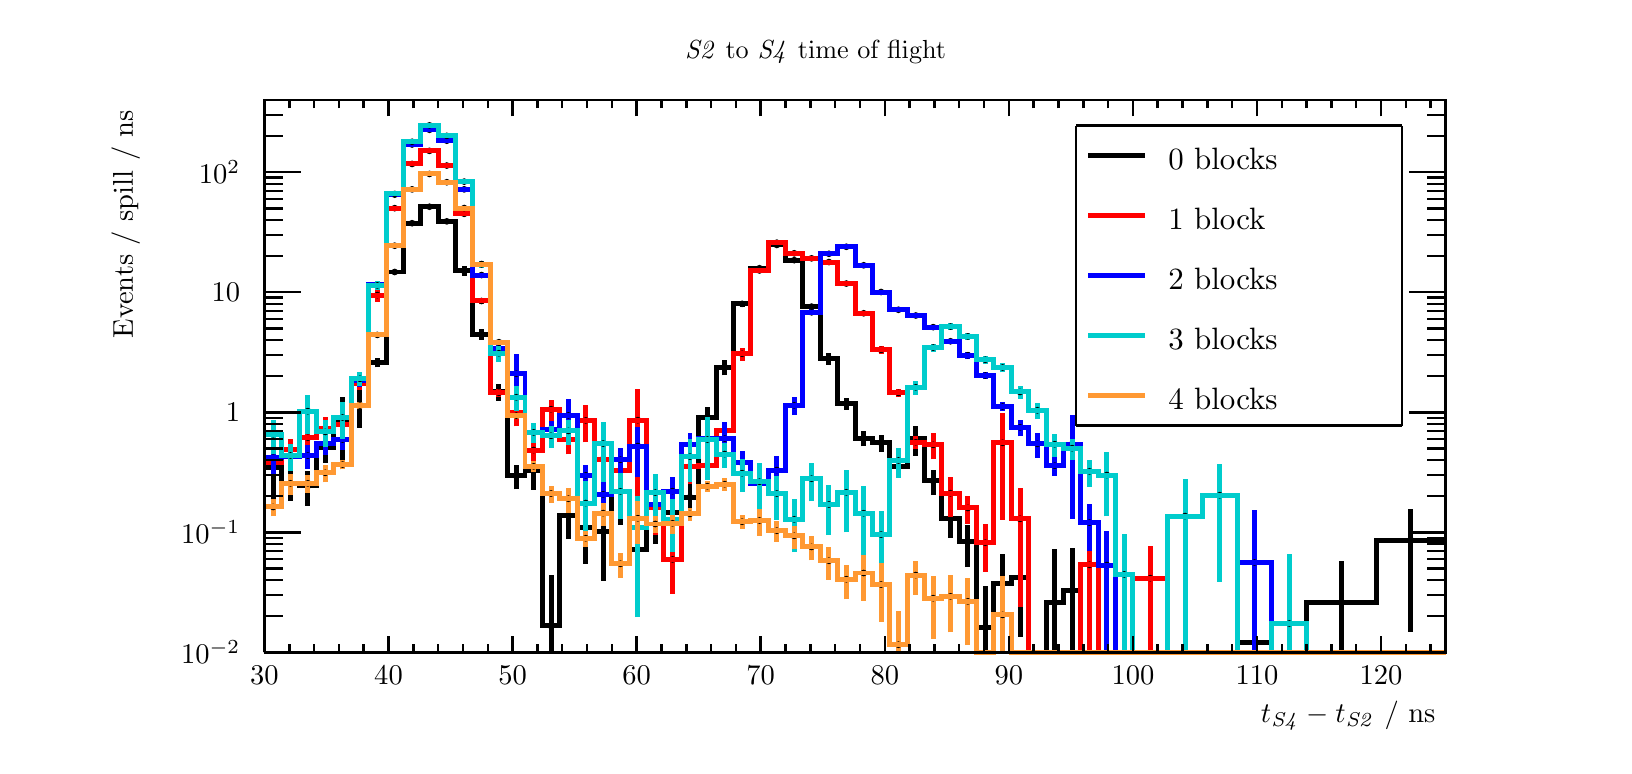
\begin{tikzpicture}
\pgfdeclareplotmark{cross} {
\pgfpathmoveto{\pgfpoint{-0.3\pgfplotmarksize}{\pgfplotmarksize}}
\pgfpathlineto{\pgfpoint{+0.3\pgfplotmarksize}{\pgfplotmarksize}}
\pgfpathlineto{\pgfpoint{+0.3\pgfplotmarksize}{0.3\pgfplotmarksize}}
\pgfpathlineto{\pgfpoint{+1\pgfplotmarksize}{0.3\pgfplotmarksize}}
\pgfpathlineto{\pgfpoint{+1\pgfplotmarksize}{-0.3\pgfplotmarksize}}
\pgfpathlineto{\pgfpoint{+0.3\pgfplotmarksize}{-0.3\pgfplotmarksize}}
\pgfpathlineto{\pgfpoint{+0.3\pgfplotmarksize}{-1.\pgfplotmarksize}}
\pgfpathlineto{\pgfpoint{-0.3\pgfplotmarksize}{-1.\pgfplotmarksize}}
\pgfpathlineto{\pgfpoint{-0.3\pgfplotmarksize}{-0.3\pgfplotmarksize}}
\pgfpathlineto{\pgfpoint{-1.\pgfplotmarksize}{-0.3\pgfplotmarksize}}
\pgfpathlineto{\pgfpoint{-1.\pgfplotmarksize}{0.3\pgfplotmarksize}}
\pgfpathlineto{\pgfpoint{-0.3\pgfplotmarksize}{0.3\pgfplotmarksize}}
\pgfpathclose
\pgfusepathqstroke
}
\pgfdeclareplotmark{cross*} {
\pgfpathmoveto{\pgfpoint{-0.3\pgfplotmarksize}{\pgfplotmarksize}}
\pgfpathlineto{\pgfpoint{+0.3\pgfplotmarksize}{\pgfplotmarksize}}
\pgfpathlineto{\pgfpoint{+0.3\pgfplotmarksize}{0.3\pgfplotmarksize}}
\pgfpathlineto{\pgfpoint{+1\pgfplotmarksize}{0.3\pgfplotmarksize}}
\pgfpathlineto{\pgfpoint{+1\pgfplotmarksize}{-0.3\pgfplotmarksize}}
\pgfpathlineto{\pgfpoint{+0.3\pgfplotmarksize}{-0.3\pgfplotmarksize}}
\pgfpathlineto{\pgfpoint{+0.3\pgfplotmarksize}{-1.\pgfplotmarksize}}
\pgfpathlineto{\pgfpoint{-0.3\pgfplotmarksize}{-1.\pgfplotmarksize}}
\pgfpathlineto{\pgfpoint{-0.3\pgfplotmarksize}{-0.3\pgfplotmarksize}}
\pgfpathlineto{\pgfpoint{-1.\pgfplotmarksize}{-0.3\pgfplotmarksize}}
\pgfpathlineto{\pgfpoint{-1.\pgfplotmarksize}{0.3\pgfplotmarksize}}
\pgfpathlineto{\pgfpoint{-0.3\pgfplotmarksize}{0.3\pgfplotmarksize}}
\pgfpathclose
\pgfusepathqfillstroke
}
\pgfdeclareplotmark{newstar} {
\pgfpathmoveto{\pgfqpoint{0pt}{\pgfplotmarksize}}
\pgfpathlineto{\pgfqpointpolar{44}{0.5\pgfplotmarksize}}
\pgfpathlineto{\pgfqpointpolar{18}{\pgfplotmarksize}}
\pgfpathlineto{\pgfqpointpolar{-20}{0.5\pgfplotmarksize}}
\pgfpathlineto{\pgfqpointpolar{-54}{\pgfplotmarksize}}
\pgfpathlineto{\pgfqpointpolar{-90}{0.5\pgfplotmarksize}}
\pgfpathlineto{\pgfqpointpolar{234}{\pgfplotmarksize}}
\pgfpathlineto{\pgfqpointpolar{198}{0.5\pgfplotmarksize}}
\pgfpathlineto{\pgfqpointpolar{162}{\pgfplotmarksize}}
\pgfpathlineto{\pgfqpointpolar{134}{0.5\pgfplotmarksize}}
\pgfpathclose
\pgfusepathqstroke
}
\pgfdeclareplotmark{newstar*} {
\pgfpathmoveto{\pgfqpoint{0pt}{\pgfplotmarksize}}
\pgfpathlineto{\pgfqpointpolar{44}{0.5\pgfplotmarksize}}
\pgfpathlineto{\pgfqpointpolar{18}{\pgfplotmarksize}}
\pgfpathlineto{\pgfqpointpolar{-20}{0.5\pgfplotmarksize}}
\pgfpathlineto{\pgfqpointpolar{-54}{\pgfplotmarksize}}
\pgfpathlineto{\pgfqpointpolar{-90}{0.5\pgfplotmarksize}}
\pgfpathlineto{\pgfqpointpolar{234}{\pgfplotmarksize}}
\pgfpathlineto{\pgfqpointpolar{198}{0.5\pgfplotmarksize}}
\pgfpathlineto{\pgfqpointpolar{162}{\pgfplotmarksize}}
\pgfpathlineto{\pgfqpointpolar{134}{0.5\pgfplotmarksize}}
\pgfpathclose
\pgfusepathqfillstroke
}
\definecolor{c}{rgb}{1,1,1};
\draw [color=c, fill=c] (0,0) rectangle (20,9.11025);
\draw [color=c, fill=c] (3,1.18433) rectangle (18,8.19923);
\definecolor{c}{rgb}{0,0,0};
\draw [c,line width=0.9] (3,1.18433) -- (3,8.19923) -- (18,8.19923) -- (18,1.18433) -- (3,1.18433);
\definecolor{c}{rgb}{1,1,1};
\draw [color=c, fill=c] (3,1.18433) rectangle (18,8.19923);
\definecolor{c}{rgb}{0,0,0};
\draw [c,line width=0.9] (3,1.18433) -- (3,8.19923) -- (18,8.19923) -- (18,1.18433) -- (3,1.18433);
\draw [c,line width=0.9] (3,1.18433) -- (3.22059,1.18433) -- (3.22059,1.18433) -- (3.44118,1.18433) -- (3.44118,1.18433) -- (3.66176,1.18433) -- (3.66176,1.18433) -- (3.88235,1.18433) -- (3.88235,1.18433) -- (4.10294,1.18433) -- (4.10294,1.18433) --
 (4.32353,1.18433) -- (4.32353,1.18433) -- (4.54412,1.18433) -- (4.54412,1.18433) -- (4.76471,1.18433) -- (4.76471,1.18433) -- (4.98529,1.18433) -- (4.98529,1.18433) -- (5.20588,1.18433) -- (5.20588,1.18433) -- (5.42647,1.18433) -- (5.42647,1.18433)
 -- (5.64706,1.18433) -- (5.64706,1.18433) -- (5.86765,1.18433) -- (5.86765,1.18433) -- (6.08824,1.18433) -- (6.08824,1.18433) -- (6.30882,1.18433) -- (6.30882,1.18433) -- (6.52941,1.18433) -- (6.52941,1.18433) -- (6.75,1.18433) -- (6.75,1.18433) --
 (6.97059,1.18433) -- (6.97059,1.18433) -- (7.19118,1.18433) -- (7.19118,1.18433) -- (7.41176,1.18433) -- (7.41176,1.18433) -- (7.63235,1.18433) -- (7.63235,1.18433) -- (7.85294,1.18433) -- (7.85294,1.18433) -- (8.07353,1.18433) -- (8.07353,1.18433)
 -- (8.29412,1.18433) -- (8.29412,1.18433) -- (8.51471,1.18433) -- (8.51471,1.18433) -- (8.73529,1.18433) -- (8.73529,1.18433) -- (8.95588,1.18433) -- (8.95588,1.18433) -- (9.17647,1.18433) -- (9.17647,1.18433) -- (9.39706,1.18433) --
 (9.39706,1.18433) -- (9.61765,1.18433) -- (9.61765,1.18433) -- (9.83823,1.18433) -- (9.83823,1.18433) -- (10.0588,1.18433) -- (10.0588,1.18433) -- (10.2794,1.18433) -- (10.2794,1.18433) -- (10.5,1.18433) -- (10.5,1.18433) -- (10.7206,1.18433) --
 (10.7206,1.18433) -- (10.9412,1.18433) -- (10.9412,1.18433) -- (11.1618,1.18433) -- (11.1618,1.18433) -- (11.3824,1.18433) -- (11.3824,1.18433) -- (11.6029,1.18433) -- (11.6029,1.18433) -- (11.8235,1.18433) -- (11.8235,1.18433) -- (12.0441,1.18433)
 -- (12.0441,1.18433) -- (12.2647,1.18433) -- (12.2647,1.18433) -- (12.4853,1.18433) -- (12.4853,1.18433) -- (12.7059,1.18433) -- (12.7059,1.18433) -- (12.9265,1.18433) -- (12.9265,1.18433) -- (13.1471,1.18433) -- (13.1471,1.18433) --
 (13.3676,1.18433) -- (13.3676,1.18433) -- (13.5882,1.18433) -- (13.5882,1.18433) -- (13.8088,1.18433) -- (13.8088,1.18433) -- (14.0294,1.18433) -- (14.0294,1.18433) -- (14.4706,1.18433) -- (14.4706,1.18433) -- (14.9118,1.18433) -- (14.9118,1.18433)
 -- (15.3529,1.18433) -- (15.3529,1.18433) -- (15.7941,1.18433) -- (15.7941,1.18433) -- (16.2353,1.18433) -- (16.2353,1.18433) -- (17.1176,1.18433) -- (17.1176,1.18433) -- (18,1.18433);
\draw [c,line width=0.9] (3,1.18433) -- (18,1.18433);
\draw [c,line width=0.9] (3,1.38931) -- (3,1.18433);
\draw [c,line width=0.9] (3.31513,1.28682) -- (3.31513,1.18433);
\draw [c,line width=0.9] (3.63025,1.28682) -- (3.63025,1.18433);
\draw [c,line width=0.9] (3.94538,1.28682) -- (3.94538,1.18433);
\draw [c,line width=0.9] (4.2605,1.28682) -- (4.2605,1.18433);
\draw [c,line width=0.9] (4.57563,1.38931) -- (4.57563,1.18433);
\draw [c,line width=0.9] (4.89076,1.28682) -- (4.89076,1.18433);
\draw [c,line width=0.9] (5.20588,1.28682) -- (5.20588,1.18433);
\draw [c,line width=0.9] (5.52101,1.28682) -- (5.52101,1.18433);
\draw [c,line width=0.9] (5.83613,1.28682) -- (5.83613,1.18433);
\draw [c,line width=0.9] (6.15126,1.38931) -- (6.15126,1.18433);
\draw [c,line width=0.9] (6.46639,1.28682) -- (6.46639,1.18433);
\draw [c,line width=0.9] (6.78151,1.28682) -- (6.78151,1.18433);
\draw [c,line width=0.9] (7.09664,1.28682) -- (7.09664,1.18433);
\draw [c,line width=0.9] (7.41176,1.28682) -- (7.41176,1.18433);
\draw [c,line width=0.9] (7.72689,1.38931) -- (7.72689,1.18433);
\draw [c,line width=0.9] (8.04202,1.28682) -- (8.04202,1.18433);
\draw [c,line width=0.9] (8.35714,1.28682) -- (8.35714,1.18433);
\draw [c,line width=0.9] (8.67227,1.28682) -- (8.67227,1.18433);
\draw [c,line width=0.9] (8.9874,1.28682) -- (8.9874,1.18433);
\draw [c,line width=0.9] (9.30252,1.38931) -- (9.30252,1.18433);
\draw [c,line width=0.9] (9.61765,1.28682) -- (9.61765,1.18433);
\draw [c,line width=0.9] (9.93277,1.28682) -- (9.93277,1.18433);
\draw [c,line width=0.9] (10.2479,1.28682) -- (10.2479,1.18433);
\draw [c,line width=0.9] (10.563,1.28682) -- (10.563,1.18433);
\draw [c,line width=0.9] (10.8782,1.38931) -- (10.8782,1.18433);
\draw [c,line width=0.9] (11.1933,1.28682) -- (11.1933,1.18433);
\draw [c,line width=0.9] (11.5084,1.28682) -- (11.5084,1.18433);
\draw [c,line width=0.9] (11.8235,1.28682) -- (11.8235,1.18433);
\draw [c,line width=0.9] (12.1387,1.28682) -- (12.1387,1.18433);
\draw [c,line width=0.9] (12.4538,1.38931) -- (12.4538,1.18433);
\draw [c,line width=0.9] (12.7689,1.28682) -- (12.7689,1.18433);
\draw [c,line width=0.9] (13.084,1.28682) -- (13.084,1.18433);
\draw [c,line width=0.9] (13.3992,1.28682) -- (13.3992,1.18433);
\draw [c,line width=0.9] (13.7143,1.28682) -- (13.7143,1.18433);
\draw [c,line width=0.9] (14.0294,1.38931) -- (14.0294,1.18433);
\draw [c,line width=0.9] (14.3445,1.28682) -- (14.3445,1.18433);
\draw [c,line width=0.9] (14.6597,1.28682) -- (14.6597,1.18433);
\draw [c,line width=0.9] (14.9748,1.28682) -- (14.9748,1.18433);
\draw [c,line width=0.9] (15.2899,1.28682) -- (15.2899,1.18433);
\draw [c,line width=0.9] (15.605,1.38931) -- (15.605,1.18433);
\draw [c,line width=0.9] (15.9202,1.28682) -- (15.9202,1.18433);
\draw [c,line width=0.9] (16.2353,1.28682) -- (16.2353,1.18433);
\draw [c,line width=0.9] (16.5504,1.28682) -- (16.5504,1.18433);
\draw [c,line width=0.9] (16.8655,1.28682) -- (16.8655,1.18433);
\draw [c,line width=0.9] (17.1807,1.38931) -- (17.1807,1.18433);
\draw [c,line width=0.9] (17.1807,1.38931) -- (17.1807,1.18433);
\draw [c,line width=0.9] (17.4958,1.28682) -- (17.4958,1.18433);
\draw [c,line width=0.9] (17.8109,1.28682) -- (17.8109,1.18433);
\draw [anchor=base] (3,0.774371) node[scale=1.03101, color=c, rotate=0]{30};
\draw [anchor=base] (4.57563,0.774371) node[scale=1.03101, color=c, rotate=0]{40};
\draw [anchor=base] (6.15126,0.774371) node[scale=1.03101, color=c, rotate=0]{50};
\draw [anchor=base] (7.72689,0.774371) node[scale=1.03101, color=c, rotate=0]{60};
\draw [anchor=base] (9.30252,0.774371) node[scale=1.03101, color=c, rotate=0]{70};
\draw [anchor=base] (10.8782,0.774371) node[scale=1.03101, color=c, rotate=0]{80};
\draw [anchor=base] (12.4538,0.774371) node[scale=1.03101, color=c, rotate=0]{90};
\draw [anchor=base] (14.0294,0.774371) node[scale=1.03101, color=c, rotate=0]{100};
\draw [anchor=base] (15.605,0.774371) node[scale=1.03101, color=c, rotate=0]{110};
\draw [anchor=base] (17.1807,0.774371) node[scale=1.03101, color=c, rotate=0]{120};
\draw [anchor= east] (18,0.382631) node[scale=1.03101, color=c, rotate=0]{$ t_{\mathit{S4}} - t_{\mathit{S2}}$ / ns};
\draw [c,line width=0.9] (3,8.19923) -- (18,8.19923);
\draw [c,line width=0.9] (3,7.99425) -- (3,8.19923);
\draw [c,line width=0.9] (3.31513,8.09674) -- (3.31513,8.19923);
\draw [c,line width=0.9] (3.63025,8.09674) -- (3.63025,8.19923);
\draw [c,line width=0.9] (3.94538,8.09674) -- (3.94538,8.19923);
\draw [c,line width=0.9] (4.2605,8.09674) -- (4.2605,8.19923);
\draw [c,line width=0.9] (4.57563,7.99425) -- (4.57563,8.19923);
\draw [c,line width=0.9] (4.89076,8.09674) -- (4.89076,8.19923);
\draw [c,line width=0.9] (5.20588,8.09674) -- (5.20588,8.19923);
\draw [c,line width=0.9] (5.52101,8.09674) -- (5.52101,8.19923);
\draw [c,line width=0.9] (5.83613,8.09674) -- (5.83613,8.19923);
\draw [c,line width=0.9] (6.15126,7.99425) -- (6.15126,8.19923);
\draw [c,line width=0.9] (6.46639,8.09674) -- (6.46639,8.19923);
\draw [c,line width=0.9] (6.78151,8.09674) -- (6.78151,8.19923);
\draw [c,line width=0.9] (7.09664,8.09674) -- (7.09664,8.19923);
\draw [c,line width=0.9] (7.41176,8.09674) -- (7.41176,8.19923);
\draw [c,line width=0.9] (7.72689,7.99425) -- (7.72689,8.19923);
\draw [c,line width=0.9] (8.04202,8.09674) -- (8.04202,8.19923);
\draw [c,line width=0.9] (8.35714,8.09674) -- (8.35714,8.19923);
\draw [c,line width=0.9] (8.67227,8.09674) -- (8.67227,8.19923);
\draw [c,line width=0.9] (8.9874,8.09674) -- (8.9874,8.19923);
\draw [c,line width=0.9] (9.30252,7.99425) -- (9.30252,8.19923);
\draw [c,line width=0.9] (9.61765,8.09674) -- (9.61765,8.19923);
\draw [c,line width=0.9] (9.93277,8.09674) -- (9.93277,8.19923);
\draw [c,line width=0.9] (10.2479,8.09674) -- (10.2479,8.19923);
\draw [c,line width=0.9] (10.563,8.09674) -- (10.563,8.19923);
\draw [c,line width=0.9] (10.8782,7.99425) -- (10.8782,8.19923);
\draw [c,line width=0.9] (11.1933,8.09674) -- (11.1933,8.19923);
\draw [c,line width=0.9] (11.5084,8.09674) -- (11.5084,8.19923);
\draw [c,line width=0.9] (11.8235,8.09674) -- (11.8235,8.19923);
\draw [c,line width=0.9] (12.1387,8.09674) -- (12.1387,8.19923);
\draw [c,line width=0.9] (12.4538,7.99425) -- (12.4538,8.19923);
\draw [c,line width=0.9] (12.7689,8.09674) -- (12.7689,8.19923);
\draw [c,line width=0.9] (13.084,8.09674) -- (13.084,8.19923);
\draw [c,line width=0.9] (13.3992,8.09674) -- (13.3992,8.19923);
\draw [c,line width=0.9] (13.7143,8.09674) -- (13.7143,8.19923);
\draw [c,line width=0.9] (14.0294,7.99425) -- (14.0294,8.19923);
\draw [c,line width=0.9] (14.3445,8.09674) -- (14.3445,8.19923);
\draw [c,line width=0.9] (14.6597,8.09674) -- (14.6597,8.19923);
\draw [c,line width=0.9] (14.9748,8.09674) -- (14.9748,8.19923);
\draw [c,line width=0.9] (15.2899,8.09674) -- (15.2899,8.19923);
\draw [c,line width=0.9] (15.605,7.99425) -- (15.605,8.19923);
\draw [c,line width=0.9] (15.9202,8.09674) -- (15.9202,8.19923);
\draw [c,line width=0.9] (16.2353,8.09674) -- (16.2353,8.19923);
\draw [c,line width=0.9] (16.5504,8.09674) -- (16.5504,8.19923);
\draw [c,line width=0.9] (16.8655,8.09674) -- (16.8655,8.19923);
\draw [c,line width=0.9] (17.1807,7.99425) -- (17.1807,8.19923);
\draw [c,line width=0.9] (17.1807,7.99425) -- (17.1807,8.19923);
\draw [c,line width=0.9] (17.4958,8.09674) -- (17.4958,8.19923);
\draw [c,line width=0.9] (17.8109,8.09674) -- (17.8109,8.19923);
\draw [c,line width=0.9] (3,1.18433) -- (3,8.19923);
\draw [c,line width=0.9] (3.462,1.18433) -- (3,1.18433);
\draw [anchor= east] (2.82,1.18433) node[scale=1.03101, color=c, rotate=0]{$10^{-2}$};
\draw [c,line width=0.9] (3.231,1.64319) -- (3,1.64319);
\draw [c,line width=0.9] (3.231,1.91161) -- (3,1.91161);
\draw [c,line width=0.9] (3.231,2.10205) -- (3,2.10205);
\draw [c,line width=0.9] (3.231,2.24977) -- (3,2.24977);
\draw [c,line width=0.9] (3.231,2.37047) -- (3,2.37047);
\draw [c,line width=0.9] (3.231,2.47251) -- (3,2.47251);
\draw [c,line width=0.9] (3.231,2.56091) -- (3,2.56091);
\draw [c,line width=0.9] (3.231,2.63888) -- (3,2.63888);
\draw [c,line width=0.9] (3.462,2.70863) -- (3,2.70863);
\draw [anchor= east] (2.82,2.70863) node[scale=1.03101, color=c, rotate=0]{$10^{-1}$};
\draw [c,line width=0.9] (3.231,3.16749) -- (3,3.16749);
\draw [c,line width=0.9] (3.231,3.4359) -- (3,3.4359);
\draw [c,line width=0.9] (3.231,3.62634) -- (3,3.62634);
\draw [c,line width=0.9] (3.231,3.77406) -- (3,3.77406);
\draw [c,line width=0.9] (3.231,3.89476) -- (3,3.89476);
\draw [c,line width=0.9] (3.231,3.99681) -- (3,3.99681);
\draw [c,line width=0.9] (3.231,4.0852) -- (3,4.0852);
\draw [c,line width=0.9] (3.231,4.16317) -- (3,4.16317);
\draw [c,line width=0.9] (3.462,4.23292) -- (3,4.23292);
\draw [anchor= east] (2.82,4.23292) node[scale=1.03101, color=c, rotate=0]{1};
\draw [c,line width=0.9] (3.231,4.69178) -- (3,4.69178);
\draw [c,line width=0.9] (3.231,4.9602) -- (3,4.9602);
\draw [c,line width=0.9] (3.231,5.15064) -- (3,5.15064);
\draw [c,line width=0.9] (3.231,5.29836) -- (3,5.29836);
\draw [c,line width=0.9] (3.231,5.41905) -- (3,5.41905);
\draw [c,line width=0.9] (3.231,5.5211) -- (3,5.5211);
\draw [c,line width=0.9] (3.231,5.6095) -- (3,5.6095);
\draw [c,line width=0.9] (3.231,5.68747) -- (3,5.68747);
\draw [c,line width=0.9] (3.462,5.75722) -- (3,5.75722);
\draw [anchor= east] (2.82,5.75722) node[scale=1.03101, color=c, rotate=0]{10};
\draw [c,line width=0.9] (3.231,6.21607) -- (3,6.21607);
\draw [c,line width=0.9] (3.231,6.48449) -- (3,6.48449);
\draw [c,line width=0.9] (3.231,6.67493) -- (3,6.67493);
\draw [c,line width=0.9] (3.231,6.82265) -- (3,6.82265);
\draw [c,line width=0.9] (3.231,6.94335) -- (3,6.94335);
\draw [c,line width=0.9] (3.231,7.04539) -- (3,7.04539);
\draw [c,line width=0.9] (3.231,7.13379) -- (3,7.13379);
\draw [c,line width=0.9] (3.231,7.21176) -- (3,7.21176);
\draw [c,line width=0.9] (3.462,7.28151) -- (3,7.28151);
\draw [anchor= east] (2.82,7.28151) node[scale=1.03101, color=c, rotate=0]{$10^{2}$};
\draw [c,line width=0.9] (3.231,7.74037) -- (3,7.74037);
\draw [c,line width=0.9] (3.231,8.00878) -- (3,8.00878);
\draw [c,line width=0.9] (3.231,8.19923) -- (3,8.19923);
\draw [anchor= east] (1.24,8.19923) node[scale=1.03101, color=c, rotate=90]{ Events / spill / ns};
\draw [c,line width=0.9] (18,1.18433) -- (18,8.19923);
\draw [c,line width=0.9] (17.538,1.18433) -- (18,1.18433);
\draw [c,line width=0.9] (17.769,1.64319) -- (18,1.64319);
\draw [c,line width=0.9] (17.769,1.91161) -- (18,1.91161);
\draw [c,line width=0.9] (17.769,2.10205) -- (18,2.10205);
\draw [c,line width=0.9] (17.769,2.24977) -- (18,2.24977);
\draw [c,line width=0.9] (17.769,2.37047) -- (18,2.37047);
\draw [c,line width=0.9] (17.769,2.47251) -- (18,2.47251);
\draw [c,line width=0.9] (17.769,2.56091) -- (18,2.56091);
\draw [c,line width=0.9] (17.769,2.63888) -- (18,2.63888);
\draw [c,line width=0.9] (17.538,2.70863) -- (18,2.70863);
\draw [c,line width=0.9] (17.769,3.16749) -- (18,3.16749);
\draw [c,line width=0.9] (17.769,3.4359) -- (18,3.4359);
\draw [c,line width=0.9] (17.769,3.62634) -- (18,3.62634);
\draw [c,line width=0.9] (17.769,3.77406) -- (18,3.77406);
\draw [c,line width=0.9] (17.769,3.89476) -- (18,3.89476);
\draw [c,line width=0.9] (17.769,3.99681) -- (18,3.99681);
\draw [c,line width=0.9] (17.769,4.0852) -- (18,4.0852);
\draw [c,line width=0.9] (17.769,4.16317) -- (18,4.16317);
\draw [c,line width=0.9] (17.538,4.23292) -- (18,4.23292);
\draw [c,line width=0.9] (17.769,4.69178) -- (18,4.69178);
\draw [c,line width=0.9] (17.769,4.9602) -- (18,4.9602);
\draw [c,line width=0.9] (17.769,5.15064) -- (18,5.15064);
\draw [c,line width=0.9] (17.769,5.29836) -- (18,5.29836);
\draw [c,line width=0.9] (17.769,5.41905) -- (18,5.41905);
\draw [c,line width=0.9] (17.769,5.5211) -- (18,5.5211);
\draw [c,line width=0.9] (17.769,5.6095) -- (18,5.6095);
\draw [c,line width=0.9] (17.769,5.68747) -- (18,5.68747);
\draw [c,line width=0.9] (17.538,5.75722) -- (18,5.75722);
\draw [c,line width=0.9] (17.769,6.21607) -- (18,6.21607);
\draw [c,line width=0.9] (17.769,6.48449) -- (18,6.48449);
\draw [c,line width=0.9] (17.769,6.67493) -- (18,6.67493);
\draw [c,line width=0.9] (17.769,6.82265) -- (18,6.82265);
\draw [c,line width=0.9] (17.769,6.94335) -- (18,6.94335);
\draw [c,line width=0.9] (17.769,7.04539) -- (18,7.04539);
\draw [c,line width=0.9] (17.769,7.13379) -- (18,7.13379);
\draw [c,line width=0.9] (17.769,7.21176) -- (18,7.21176);
\draw [c,line width=0.9] (17.538,7.28151) -- (18,7.28151);
\draw [c,line width=0.9] (17.769,7.74037) -- (18,7.74037);
\draw [c,line width=0.9] (17.769,8.00878) -- (18,8.00878);
\draw [c,line width=0.9] (17.769,8.19923) -- (18,8.19923);
\draw [c,line width=1.8] (3.11029,3.01059) -- (3.11029,3.53716);
\draw [c,line width=1.8] (3.11029,3.53716) -- (3.11029,3.82669);
\foreach \P in {(3.11029,3.53716)}{\draw[mark options={color=c,fill=c},mark size=2.402402pt,mark=*,mark size=1pt] plot coordinates {\P};}
\draw [c,line width=1.8] (3.33088,3.11042) -- (3.33088,3.3234);
\draw [c,line width=1.8] (3.33088,3.3234) -- (3.33088,3.48428);
\foreach \P in {(3.33088,3.3234)}{\draw[mark options={color=c,fill=c},mark size=2.402402pt,mark=*,mark size=1pt] plot coordinates {\P};}
\draw [c,line width=1.8] (3.55147,3.04626) -- (3.55147,3.29901);
\draw [c,line width=1.8] (3.55147,3.29901) -- (3.55147,3.48149);
\foreach \P in {(3.55147,3.29901)}{\draw[mark options={color=c,fill=c},mark size=2.402402pt,mark=*,mark size=1pt] plot coordinates {\P};}
\draw [c,line width=1.8] (3.77206,3.59376) -- (3.77206,3.78886);
\draw [c,line width=1.8] (3.77206,3.78886) -- (3.77206,3.93936);
\foreach \P in {(3.77206,3.78886)}{\draw[mark options={color=c,fill=c},mark size=2.402402pt,mark=*,mark size=1pt] plot coordinates {\P};}
\draw [c,line width=1.8] (3.99265,3.50647) -- (3.99265,4.11906);
\draw [c,line width=1.8] (3.99265,4.11906) -- (3.99265,4.4317);
\foreach \P in {(3.99265,4.11906)}{\draw[mark options={color=c,fill=c},mark size=2.402402pt,mark=*,mark size=1pt] plot coordinates {\P};}
\draw [c,line width=1.8] (4.21324,4.03848) -- (4.21324,4.32444);
\draw [c,line width=1.8] (4.21324,4.32444) -- (4.21324,4.52349);
\foreach \P in {(4.21324,4.32444)}{\draw[mark options={color=c,fill=c},mark size=2.402402pt,mark=*,mark size=1pt] plot coordinates {\P};}
\draw [c,line width=1.8] (4.43382,4.80441) -- (4.43382,4.86726);
\draw [c,line width=1.8] (4.43382,4.86726) -- (4.43382,4.92466);
\foreach \P in {(4.43382,4.86726)}{\draw[mark options={color=c,fill=c},mark size=2.402402pt,mark=*,mark size=1pt] plot coordinates {\P};}
\draw [c,line width=1.8] (4.65441,5.98509) -- (4.65441,6.01435);
\draw [c,line width=1.8] (4.65441,6.01435) -- (4.65441,6.04237);
\foreach \P in {(4.65441,6.01435)}{\draw[mark options={color=c,fill=c},mark size=2.402402pt,mark=*,mark size=1pt] plot coordinates {\P};}
\draw [c,line width=1.8] (4.875,6.6125) -- (4.875,6.63394);
\draw [c,line width=1.8] (4.875,6.63394) -- (4.875,6.65471);
\foreach \P in {(4.875,6.63394)}{\draw[mark options={color=c,fill=c},mark size=2.402402pt,mark=*,mark size=1pt] plot coordinates {\P};}
\draw [c,line width=1.8] (5.09559,6.82128) -- (5.09559,6.84324);
\draw [c,line width=1.8] (5.09559,6.84324) -- (5.09559,6.8645);
\foreach \P in {(5.09559,6.84324)}{\draw[mark options={color=c,fill=c},mark size=2.402402pt,mark=*,mark size=1pt] plot coordinates {\P};}
\draw [c,line width=1.8] (5.31618,6.62665) -- (5.31618,6.65758);
\draw [c,line width=1.8] (5.31618,6.65758) -- (5.31618,6.68713);
\foreach \P in {(5.31618,6.65758)}{\draw[mark options={color=c,fill=c},mark size=2.402402pt,mark=*,mark size=1pt] plot coordinates {\P};}
\draw [c,line width=1.8] (5.53676,5.96974) -- (5.53676,6.02947);
\draw [c,line width=1.8] (5.53676,6.02947) -- (5.53676,6.08426);
\foreach \P in {(5.53676,6.02947)}{\draw[mark options={color=c,fill=c},mark size=2.402402pt,mark=*,mark size=1pt] plot coordinates {\P};}
\draw [c,line width=1.8] (5.75735,5.15161) -- (5.75735,5.22451);
\draw [c,line width=1.8] (5.75735,5.22451) -- (5.75735,5.29016);
\foreach \P in {(5.75735,5.22451)}{\draw[mark options={color=c,fill=c},mark size=2.402402pt,mark=*,mark size=1pt] plot coordinates {\P};}
\draw [c,line width=1.8] (5.97794,4.37808) -- (5.97794,4.49492);
\draw [c,line width=1.8] (5.97794,4.49492) -- (5.97794,4.5942);
\foreach \P in {(5.97794,4.49492)}{\draw[mark options={color=c,fill=c},mark size=2.402402pt,mark=*,mark size=1pt] plot coordinates {\P};}
\draw [c,line width=1.8] (6.19853,3.25269) -- (6.19853,3.42437);
\draw [c,line width=1.8] (6.19853,3.42437) -- (6.19853,3.56058);
\foreach \P in {(6.19853,3.42437)}{\draw[mark options={color=c,fill=c},mark size=2.402402pt,mark=*,mark size=1pt] plot coordinates {\P};}
\draw [c,line width=1.8] (6.41912,3.25055) -- (6.41912,3.49418);
\draw [c,line width=1.8] (6.41912,3.49418) -- (6.41912,3.67187);
\foreach \P in {(6.41912,3.49418)}{\draw[mark options={color=c,fill=c},mark size=2.402402pt,mark=*,mark size=1pt] plot coordinates {\P};}
\draw [c,line width=1.8] (6.63971,1.18433) -- (6.63971,1.52013);
\draw [c,line width=1.8] (6.63971,1.52013) -- (6.63971,2.16651);
\foreach \P in {(6.63971,1.52013)}{\draw[mark options={color=c,fill=c},mark size=2.402402pt,mark=*,mark size=1pt] plot coordinates {\P};}
\draw [c,line width=1.8] (6.86029,2.6208) -- (6.86029,2.92257);
\draw [c,line width=1.8] (6.86029,2.92257) -- (6.86029,3.12908);
\foreach \P in {(6.86029,2.92257)}{\draw[mark options={color=c,fill=c},mark size=2.402402pt,mark=*,mark size=1pt] plot coordinates {\P};}
\draw [c,line width=1.8] (7.08088,2.30724) -- (7.08088,2.76685);
\draw [c,line width=1.8] (7.08088,2.76685) -- (7.08088,3.03552);
\foreach \P in {(7.08088,2.76685)}{\draw[mark options={color=c,fill=c},mark size=2.402402pt,mark=*,mark size=1pt] plot coordinates {\P};}
\draw [c,line width=1.8] (7.30147,2.09583) -- (7.30147,2.71841);
\draw [c,line width=1.8] (7.30147,2.71841) -- (7.30147,3.03349);
\foreach \P in {(7.30147,2.71841)}{\draw[mark options={color=c,fill=c},mark size=2.402402pt,mark=*,mark size=1pt] plot coordinates {\P};}
\draw [c,line width=1.8] (7.52206,2.80159) -- (7.52206,3.22686);
\draw [c,line width=1.8] (7.52206,3.22686) -- (7.52206,3.48368);
\foreach \P in {(7.52206,3.22686)}{\draw[mark options={color=c,fill=c},mark size=2.402402pt,mark=*,mark size=1pt] plot coordinates {\P};}
\draw [c,line width=1.8] (7.74265,2.00764) -- (7.74265,2.49321);
\draw [c,line width=1.8] (7.74265,2.49321) -- (7.74265,2.7703);
\foreach \P in {(7.74265,2.49321)}{\draw[mark options={color=c,fill=c},mark size=2.402402pt,mark=*,mark size=1pt] plot coordinates {\P};}
\draw [c,line width=1.8] (7.96324,2.55851) -- (7.96324,3.02649);
\draw [c,line width=1.8] (7.96324,3.02649) -- (7.96324,3.29792);
\foreach \P in {(7.96324,3.02649)}{\draw[mark options={color=c,fill=c},mark size=2.402402pt,mark=*,mark size=1pt] plot coordinates {\P};}
\draw [c,line width=1.8] (8.18382,2.65833) -- (8.18382,2.95996);
\draw [c,line width=1.8] (8.18382,2.95996) -- (8.18382,3.16641);
\foreach \P in {(8.18382,2.95996)}{\draw[mark options={color=c,fill=c},mark size=2.402402pt,mark=*,mark size=1pt] plot coordinates {\P};}
\draw [c,line width=1.8] (8.40441,2.93473) -- (8.40441,3.15503);
\draw [c,line width=1.8] (8.40441,3.15503) -- (8.40441,3.32004);
\foreach \P in {(8.40441,3.15503)}{\draw[mark options={color=c,fill=c},mark size=2.402402pt,mark=*,mark size=1pt] plot coordinates {\P};}
\draw [c,line width=1.8] (8.625,4.01263) -- (8.625,4.17078);
\draw [c,line width=1.8] (8.625,4.17078) -- (8.625,4.29834);
\foreach \P in {(8.625,4.17078)}{\draw[mark options={color=c,fill=c},mark size=2.402402pt,mark=*,mark size=1pt] plot coordinates {\P};}
\draw [c,line width=1.8] (8.84559,4.70224) -- (8.84559,4.8068);
\draw [c,line width=1.8] (8.84559,4.8068) -- (8.84559,4.89707);
\foreach \P in {(8.84559,4.8068)}{\draw[mark options={color=c,fill=c},mark size=2.402402pt,mark=*,mark size=1pt] plot coordinates {\P};}
\draw [c,line width=1.8] (9.06618,5.56733) -- (9.06618,5.6099);
\draw [c,line width=1.8] (9.06618,5.6099) -- (9.06618,5.64989);
\foreach \P in {(9.06618,5.6099)}{\draw[mark options={color=c,fill=c},mark size=2.402402pt,mark=*,mark size=1pt] plot coordinates {\P};}
\draw [c,line width=1.8] (9.28677,6.03393) -- (9.28677,6.06192);
\draw [c,line width=1.8] (9.28677,6.06192) -- (9.28677,6.08878);
\foreach \P in {(9.28677,6.06192)}{\draw[mark options={color=c,fill=c},mark size=2.402402pt,mark=*,mark size=1pt] plot coordinates {\P};}
\draw [c,line width=1.8] (9.50735,6.33726) -- (9.50735,6.35795);
\draw [c,line width=1.8] (9.50735,6.35795) -- (9.50735,6.37801);
\foreach \P in {(9.50735,6.35795)}{\draw[mark options={color=c,fill=c},mark size=2.402402pt,mark=*,mark size=1pt] plot coordinates {\P};}
\draw [c,line width=1.8] (9.72794,6.14261) -- (9.72794,6.16458);
\draw [c,line width=1.8] (9.72794,6.16458) -- (9.72794,6.18584);
\foreach \P in {(9.72794,6.16458)}{\draw[mark options={color=c,fill=c},mark size=2.402402pt,mark=*,mark size=1pt] plot coordinates {\P};}
\draw [c,line width=1.8] (9.94853,5.53971) -- (9.94853,5.57486);
\draw [c,line width=1.8] (9.94853,5.57486) -- (9.94853,5.60823);
\foreach \P in {(9.94853,5.57486)}{\draw[mark options={color=c,fill=c},mark size=2.402402pt,mark=*,mark size=1pt] plot coordinates {\P};}
\draw [c,line width=1.8] (10.1691,4.83738) -- (10.1691,4.9182);
\draw [c,line width=1.8] (10.1691,4.9182) -- (10.1691,4.99022);
\foreach \P in {(10.1691,4.9182)}{\draw[mark options={color=c,fill=c},mark size=2.402402pt,mark=*,mark size=1pt] plot coordinates {\P};}
\draw [c,line width=1.8] (10.3897,4.26375) -- (10.3897,4.33999);
\draw [c,line width=1.8] (10.3897,4.33999) -- (10.3897,4.40834);
\foreach \P in {(10.3897,4.33999)}{\draw[mark options={color=c,fill=c},mark size=2.402402pt,mark=*,mark size=1pt] plot coordinates {\P};}
\draw [c,line width=1.8] (10.6103,3.79985) -- (10.6103,3.9013);
\draw [c,line width=1.8] (10.6103,3.9013) -- (10.6103,3.98925);
\foreach \P in {(10.6103,3.9013)}{\draw[mark options={color=c,fill=c},mark size=2.402402pt,mark=*,mark size=1pt] plot coordinates {\P};}
\draw [c,line width=1.8] (10.8309,3.72814) -- (10.8309,3.84562);
\draw [c,line width=1.8] (10.8309,3.84562) -- (10.8309,3.94536);
\foreach \P in {(10.8309,3.84562)}{\draw[mark options={color=c,fill=c},mark size=2.402402pt,mark=*,mark size=1pt] plot coordinates {\P};}
\draw [c,line width=1.8] (11.0515,3.40787) -- (11.0515,3.53943);
\draw [c,line width=1.8] (11.0515,3.53943) -- (11.0515,3.64913);
\foreach \P in {(11.0515,3.53943)}{\draw[mark options={color=c,fill=c},mark size=2.402402pt,mark=*,mark size=1pt] plot coordinates {\P};}
\draw [c,line width=1.8] (11.2721,3.6794) -- (11.2721,3.89767);
\draw [c,line width=1.8] (11.2721,3.89767) -- (11.2721,4.06153);
\foreach \P in {(11.2721,3.89767)}{\draw[mark options={color=c,fill=c},mark size=2.402402pt,mark=*,mark size=1pt] plot coordinates {\P};}
\draw [c,line width=1.8] (11.4926,3.17961) -- (11.4926,3.36034);
\draw [c,line width=1.8] (11.4926,3.36034) -- (11.4926,3.50216);
\foreach \P in {(11.4926,3.36034)}{\draw[mark options={color=c,fill=c},mark size=2.402402pt,mark=*,mark size=1pt] plot coordinates {\P};}
\draw [c,line width=1.8] (11.7132,2.64028) -- (11.7132,2.88433);
\draw [c,line width=1.8] (11.7132,2.88433) -- (11.7132,3.06225);
\foreach \P in {(11.7132,2.88433)}{\draw[mark options={color=c,fill=c},mark size=2.402402pt,mark=*,mark size=1pt] plot coordinates {\P};}
\draw [c,line width=1.8] (11.9338,2.26532) -- (11.9338,2.59007);
\draw [c,line width=1.8] (11.9338,2.59007) -- (11.9338,2.80697);
\foreach \P in {(11.9338,2.59007)}{\draw[mark options={color=c,fill=c},mark size=2.402402pt,mark=*,mark size=1pt] plot coordinates {\P};}
\draw [c,line width=1.8] (12.1544,1.18433) -- (12.1544,1.50181);
\draw [c,line width=1.8] (12.1544,1.50181) -- (12.1544,2.02432);
\foreach \P in {(12.1544,1.50181)}{\draw[mark options={color=c,fill=c},mark size=2.402402pt,mark=*,mark size=1pt] plot coordinates {\P};}
\draw [c,line width=1.8] (12.375,1.18433) -- (12.375,2.05707);
\draw [c,line width=1.8] (12.375,2.05707) -- (12.375,2.42814);
\foreach \P in {(12.375,2.05707)}{\draw[mark options={color=c,fill=c},mark size=2.402402pt,mark=*,mark size=1pt] plot coordinates {\P};}
\draw [c,line width=1.8] (12.5956,1.38032) -- (12.5956,2.13491);
\draw [c,line width=1.8] (12.5956,2.13491) -- (12.5956,2.4784);
\foreach \P in {(12.5956,2.13491)}{\draw[mark options={color=c,fill=c},mark size=2.402402pt,mark=*,mark size=1pt] plot coordinates {\P};}
\draw [c,line width=1.8] (13.0368,1.18433) -- (13.0368,1.81278);
\draw [c,line width=1.8] (13.0368,1.81278) -- (13.0368,2.49098);
\foreach \P in {(13.0368,1.81278)}{\draw[mark options={color=c,fill=c},mark size=2.402402pt,mark=*,mark size=1pt] plot coordinates {\P};}
\draw [c,line width=1.8] (13.2574,1.18433) -- (13.2574,1.96775);
\draw [c,line width=1.8] (13.2574,1.96775) -- (13.2574,2.508);
\foreach \P in {(13.2574,1.96775)}{\draw[mark options={color=c,fill=c},mark size=2.402402pt,mark=*,mark size=1pt] plot coordinates {\P};}
\draw [c,line width=1.8] (15.5735,1.18433) -- (15.5735,1.30488);
\draw [c,line width=1.8] (15.5735,1.30488) -- (15.5735,2.1569);
\foreach \P in {(15.5735,1.30488)}{\draw[mark options={color=c,fill=c},mark size=2.402402pt,mark=*,mark size=1pt] plot coordinates {\P};}
\draw [c,line width=1.8] (16.6765,1.18433) -- (16.6765,1.81474);
\draw [c,line width=1.8] (16.6765,1.81474) -- (16.6765,2.34592);
\foreach \P in {(16.6765,1.81474)}{\draw[mark options={color=c,fill=c},mark size=2.402402pt,mark=*,mark size=1pt] plot coordinates {\P};}
\draw [c,line width=1.8] (17.5588,1.44788) -- (17.5588,2.60963);
\draw [c,line width=1.8] (17.5588,2.60963) -- (17.5588,3.00863);
\foreach \P in {(17.5588,2.60963)}{\draw[mark options={color=c,fill=c},mark size=2.402402pt,mark=*,mark size=1pt] plot coordinates {\P};}
\draw [c,line width=1.8] (3,3.53716) -- (3.22059,3.53716) -- (3.22059,3.3234) -- (3.44118,3.3234) -- (3.44118,3.29901) -- (3.66176,3.29901) -- (3.66176,3.78886) -- (3.88235,3.78886) -- (3.88235,4.11906) -- (4.10294,4.11906) -- (4.10294,4.32444) --
 (4.32353,4.32444) -- (4.32353,4.86726) -- (4.54412,4.86726) -- (4.54412,6.01435) -- (4.76471,6.01435) -- (4.76471,6.63394) -- (4.98529,6.63394) -- (4.98529,6.84324) -- (5.20588,6.84324) -- (5.20588,6.65758) -- (5.42647,6.65758) -- (5.42647,6.02947)
 -- (5.64706,6.02947) -- (5.64706,5.22451) -- (5.86765,5.22451) -- (5.86765,4.49492) -- (6.08824,4.49492) -- (6.08824,3.42437) -- (6.30882,3.42437) -- (6.30882,3.49418) -- (6.52941,3.49418) -- (6.52941,1.52013) -- (6.75,1.52013) -- (6.75,2.92257) --
 (6.97059,2.92257) -- (6.97059,2.76685) -- (7.19118,2.76685) -- (7.19118,2.71841) -- (7.41176,2.71841) -- (7.41176,3.22686) -- (7.63235,3.22686) -- (7.63235,2.49321) -- (7.85294,2.49321) -- (7.85294,3.02649) -- (8.07353,3.02649) -- (8.07353,2.95996)
 -- (8.29412,2.95996) -- (8.29412,3.15503) -- (8.51471,3.15503) -- (8.51471,4.17078) -- (8.73529,4.17078) -- (8.73529,4.8068) -- (8.95588,4.8068) -- (8.95588,5.6099) -- (9.17647,5.6099) -- (9.17647,6.06192) -- (9.39706,6.06192) -- (9.39706,6.35795)
 -- (9.61765,6.35795) -- (9.61765,6.16458) -- (9.83823,6.16458) -- (9.83823,5.57486) -- (10.0588,5.57486) -- (10.0588,4.9182) -- (10.2794,4.9182) -- (10.2794,4.33999) -- (10.5,4.33999) -- (10.5,3.9013) -- (10.7206,3.9013) -- (10.7206,3.84562) --
 (10.9412,3.84562) -- (10.9412,3.53943) -- (11.1618,3.53943) -- (11.1618,3.89767) -- (11.3824,3.89767) -- (11.3824,3.36034) -- (11.6029,3.36034) -- (11.6029,2.88433) -- (11.8235,2.88433) -- (11.8235,2.59007) -- (12.0441,2.59007) -- (12.0441,1.50181)
 -- (12.2647,1.50181) -- (12.2647,2.05707) -- (12.4853,2.05707) -- (12.4853,2.13491) -- (12.7059,2.13491) -- (12.7059,1.18433) -- (12.9265,1.18433) -- (12.9265,1.81278) -- (13.1471,1.81278) -- (13.1471,1.96775) -- (13.3676,1.96775) --
 (13.3676,1.18433) -- (13.5882,1.18433) -- (13.5882,1.18433) -- (13.8088,1.18433) -- (13.8088,1.18433) -- (14.0294,1.18433) -- (14.0294,1.18433) -- (14.4706,1.18433) -- (14.4706,1.18433) -- (14.9118,1.18433) -- (14.9118,1.18433) -- (15.3529,1.18433)
 -- (15.3529,1.30488) -- (15.7941,1.30488) -- (15.7941,1.18433) -- (16.2353,1.18433) -- (16.2353,1.81474) -- (17.1176,1.81474) -- (17.1176,2.60963) -- (18,2.60963);
\definecolor{c}{rgb}{1,0,0};
\draw [c,line width=1.8] (3.11029,3.43417) -- (3.11029,3.59745);
\draw [c,line width=1.8] (3.11029,3.59745) -- (3.11029,3.72833);
\definecolor{c}{rgb}{0,0,0};
\foreach \P in {(3.11029,3.59745)}{\draw[mark options={color=c,fill=c},mark size=2.402402pt,mark=*,mark size=1pt] plot coordinates {\P};}
\definecolor{c}{rgb}{1,0,0};
\draw [c,line width=1.8] (3.33088,3.59527) -- (3.33088,3.75848);
\draw [c,line width=1.8] (3.33088,3.75848) -- (3.33088,3.8893);
\definecolor{c}{rgb}{0,0,0};
\foreach \P in {(3.33088,3.75848)}{\draw[mark options={color=c,fill=c},mark size=2.402402pt,mark=*,mark size=1pt] plot coordinates {\P};}
\definecolor{c}{rgb}{1,0,0};
\draw [c,line width=1.8] (3.55147,3.71147) -- (3.55147,3.90953);
\draw [c,line width=1.8] (3.55147,3.90953) -- (3.55147,4.06178);
\definecolor{c}{rgb}{0,0,0};
\foreach \P in {(3.55147,3.90953)}{\draw[mark options={color=c,fill=c},mark size=2.402402pt,mark=*,mark size=1pt] plot coordinates {\P};}
\definecolor{c}{rgb}{1,0,0};
\draw [c,line width=1.8] (3.77206,3.85441) -- (3.77206,4.0293);
\draw [c,line width=1.8] (3.77206,4.0293) -- (3.77206,4.16751);
\definecolor{c}{rgb}{0,0,0};
\foreach \P in {(3.77206,4.0293)}{\draw[mark options={color=c,fill=c},mark size=2.402402pt,mark=*,mark size=1pt] plot coordinates {\P};}
\definecolor{c}{rgb}{1,0,0};
\draw [c,line width=1.8] (3.99265,3.95332) -- (3.99265,4.08156);
\draw [c,line width=1.8] (3.99265,4.08156) -- (3.99265,4.18895);
\definecolor{c}{rgb}{0,0,0};
\foreach \P in {(3.99265,4.08156)}{\draw[mark options={color=c,fill=c},mark size=2.402402pt,mark=*,mark size=1pt] plot coordinates {\P};}
\definecolor{c}{rgb}{1,0,0};
\draw [c,line width=1.8] (4.21324,4.52071) -- (4.21324,4.59954);
\draw [c,line width=1.8] (4.21324,4.59954) -- (4.21324,4.66997);
\definecolor{c}{rgb}{0,0,0};
\foreach \P in {(4.21324,4.59954)}{\draw[mark options={color=c,fill=c},mark size=2.402402pt,mark=*,mark size=1pt] plot coordinates {\P};}
\definecolor{c}{rgb}{1,0,0};
\draw [c,line width=1.8] (4.43382,5.63827) -- (4.43382,5.72107);
\draw [c,line width=1.8] (4.43382,5.72107) -- (4.43382,5.79465);
\definecolor{c}{rgb}{0,0,0};
\foreach \P in {(4.43382,5.72107)}{\draw[mark options={color=c,fill=c},mark size=2.402402pt,mark=*,mark size=1pt] plot coordinates {\P};}
\definecolor{c}{rgb}{1,0,0};
\draw [c,line width=1.8] (4.65441,6.81052) -- (4.65441,6.825);
\draw [c,line width=1.8] (4.65441,6.825) -- (4.65441,6.83917);
\definecolor{c}{rgb}{0,0,0};
\foreach \P in {(4.65441,6.825)}{\draw[mark options={color=c,fill=c},mark size=2.402402pt,mark=*,mark size=1pt] plot coordinates {\P};}
\definecolor{c}{rgb}{1,0,0};
\draw [c,line width=1.8] (4.875,7.37651) -- (4.875,7.38652);
\draw [c,line width=1.8] (4.875,7.38652) -- (4.875,7.39638);
\definecolor{c}{rgb}{0,0,0};
\foreach \P in {(4.875,7.38652)}{\draw[mark options={color=c,fill=c},mark size=2.402402pt,mark=*,mark size=1pt] plot coordinates {\P};}
\definecolor{c}{rgb}{1,0,0};
\draw [c,line width=1.8] (5.09559,7.54287) -- (5.09559,7.55278);
\draw [c,line width=1.8] (5.09559,7.55278) -- (5.09559,7.56253);
\definecolor{c}{rgb}{0,0,0};
\foreach \P in {(5.09559,7.55278)}{\draw[mark options={color=c,fill=c},mark size=2.402402pt,mark=*,mark size=1pt] plot coordinates {\P};}
\definecolor{c}{rgb}{1,0,0};
\draw [c,line width=1.8] (5.31618,7.3552) -- (5.31618,7.36619);
\draw [c,line width=1.8] (5.31618,7.36619) -- (5.31618,7.37701);
\definecolor{c}{rgb}{0,0,0};
\foreach \P in {(5.31618,7.36619)}{\draw[mark options={color=c,fill=c},mark size=2.402402pt,mark=*,mark size=1pt] plot coordinates {\P};}
\definecolor{c}{rgb}{1,0,0};
\draw [c,line width=1.8] (5.53676,6.73277) -- (5.53676,6.75315);
\draw [c,line width=1.8] (5.53676,6.75315) -- (5.53676,6.77292);
\definecolor{c}{rgb}{0,0,0};
\foreach \P in {(5.53676,6.75315)}{\draw[mark options={color=c,fill=c},mark size=2.402402pt,mark=*,mark size=1pt] plot coordinates {\P};}
\definecolor{c}{rgb}{1,0,0};
\draw [c,line width=1.8] (5.75735,5.60394) -- (5.75735,5.6462);
\draw [c,line width=1.8] (5.75735,5.6462) -- (5.75735,5.68592);
\definecolor{c}{rgb}{0,0,0};
\foreach \P in {(5.75735,5.6462)}{\draw[mark options={color=c,fill=c},mark size=2.402402pt,mark=*,mark size=1pt] plot coordinates {\P};}
\definecolor{c}{rgb}{1,0,0};
\draw [c,line width=1.8] (5.97794,4.4251) -- (5.97794,4.4799);
\draw [c,line width=1.8] (5.97794,4.4799) -- (5.97794,4.5305);
\definecolor{c}{rgb}{0,0,0};
\foreach \P in {(5.97794,4.4799)}{\draw[mark options={color=c,fill=c},mark size=2.402402pt,mark=*,mark size=1pt] plot coordinates {\P};}
\definecolor{c}{rgb}{1,0,0};
\draw [c,line width=1.8] (6.19853,4.05334) -- (6.19853,4.23302);
\draw [c,line width=1.8] (6.19853,4.23302) -- (6.19853,4.3742);
\definecolor{c}{rgb}{0,0,0};
\foreach \P in {(6.19853,4.23302)}{\draw[mark options={color=c,fill=c},mark size=2.402402pt,mark=*,mark size=1pt] plot coordinates {\P};}
\definecolor{c}{rgb}{1,0,0};
\draw [c,line width=1.8] (6.41912,3.59453) -- (6.41912,3.75337);
\draw [c,line width=1.8] (6.41912,3.75337) -- (6.41912,3.88137);
\definecolor{c}{rgb}{0,0,0};
\foreach \P in {(6.41912,3.75337)}{\draw[mark options={color=c,fill=c},mark size=2.402402pt,mark=*,mark size=1pt] plot coordinates {\P};}
\definecolor{c}{rgb}{1,0,0};
\draw [c,line width=1.8] (6.63971,4.12399) -- (6.63971,4.27218);
\draw [c,line width=1.8] (6.63971,4.27218) -- (6.63971,4.39319);
\definecolor{c}{rgb}{0,0,0};
\foreach \P in {(6.63971,4.27218)}{\draw[mark options={color=c,fill=c},mark size=2.402402pt,mark=*,mark size=1pt] plot coordinates {\P};}
\definecolor{c}{rgb}{1,0,0};
\draw [c,line width=1.8] (6.86029,3.69891) -- (6.86029,3.89058);
\draw [c,line width=1.8] (6.86029,3.89058) -- (6.86029,4.03903);
\definecolor{c}{rgb}{0,0,0};
\foreach \P in {(6.86029,3.89058)}{\draw[mark options={color=c,fill=c},mark size=2.402402pt,mark=*,mark size=1pt] plot coordinates {\P};}
\definecolor{c}{rgb}{1,0,0};
\draw [c,line width=1.8] (7.08088,3.85026) -- (7.08088,4.12965);
\draw [c,line width=1.8] (7.08088,4.12965) -- (7.08088,4.32552);
\definecolor{c}{rgb}{0,0,0};
\foreach \P in {(7.08088,4.12965)}{\draw[mark options={color=c,fill=c},mark size=2.402402pt,mark=*,mark size=1pt] plot coordinates {\P};}
\definecolor{c}{rgb}{1,0,0};
\draw [c,line width=1.8] (7.30147,3.2741) -- (7.30147,3.63866);
\draw [c,line width=1.8] (7.30147,3.63866) -- (7.30147,3.87241);
\definecolor{c}{rgb}{0,0,0};
\foreach \P in {(7.30147,3.63866)}{\draw[mark options={color=c,fill=c},mark size=2.402402pt,mark=*,mark size=1pt] plot coordinates {\P};}
\definecolor{c}{rgb}{1,0,0};
\draw [c,line width=1.8] (7.52206,3.1868) -- (7.52206,3.49872);
\draw [c,line width=1.8] (7.52206,3.49872) -- (7.52206,3.70988);
\definecolor{c}{rgb}{0,0,0};
\foreach \P in {(7.52206,3.49872)}{\draw[mark options={color=c,fill=c},mark size=2.402402pt,mark=*,mark size=1pt] plot coordinates {\P};}
\definecolor{c}{rgb}{1,0,0};
\draw [c,line width=1.8] (7.74265,3.01136) -- (7.74265,4.13272);
\draw [c,line width=1.8] (7.74265,4.13272) -- (7.74265,4.52777);
\definecolor{c}{rgb}{0,0,0};
\foreach \P in {(7.74265,4.13272)}{\draw[mark options={color=c,fill=c},mark size=2.402402pt,mark=*,mark size=1pt] plot coordinates {\P};}
\definecolor{c}{rgb}{1,0,0};
\draw [c,line width=1.8] (7.96324,2.67344) -- (7.96324,3.01927);
\draw [c,line width=1.8] (7.96324,3.01927) -- (7.96324,3.24527);
\definecolor{c}{rgb}{0,0,0};
\foreach \P in {(7.96324,3.01927)}{\draw[mark options={color=c,fill=c},mark size=2.402402pt,mark=*,mark size=1pt] plot coordinates {\P};}
\definecolor{c}{rgb}{1,0,0};
\draw [c,line width=1.8] (8.18382,1.92623) -- (8.18382,2.36405);
\draw [c,line width=1.8] (8.18382,2.36405) -- (8.18382,2.6253);
\definecolor{c}{rgb}{0,0,0};
\foreach \P in {(8.18382,2.36405)}{\draw[mark options={color=c,fill=c},mark size=2.402402pt,mark=*,mark size=1pt] plot coordinates {\P};}
\definecolor{c}{rgb}{1,0,0};
\draw [c,line width=1.8] (8.40441,3.32695) -- (8.40441,3.5452);
\draw [c,line width=1.8] (8.40441,3.5452) -- (8.40441,3.70907);
\definecolor{c}{rgb}{0,0,0};
\foreach \P in {(8.40441,3.5452)}{\draw[mark options={color=c,fill=c},mark size=2.402402pt,mark=*,mark size=1pt] plot coordinates {\P};}
\definecolor{c}{rgb}{1,0,0};
\draw [c,line width=1.8] (8.625,3.42251) -- (8.625,3.56238);
\draw [c,line width=1.8] (8.625,3.56238) -- (8.625,3.67779);
\definecolor{c}{rgb}{0,0,0};
\foreach \P in {(8.625,3.56238)}{\draw[mark options={color=c,fill=c},mark size=2.402402pt,mark=*,mark size=1pt] plot coordinates {\P};}
\definecolor{c}{rgb}{1,0,0};
\draw [c,line width=1.8] (8.84559,3.87501) -- (8.84559,3.99748);
\draw [c,line width=1.8] (8.84559,3.99748) -- (8.84559,4.1008);
\definecolor{c}{rgb}{0,0,0};
\foreach \P in {(8.84559,3.99748)}{\draw[mark options={color=c,fill=c},mark size=2.402402pt,mark=*,mark size=1pt] plot coordinates {\P};}
\definecolor{c}{rgb}{1,0,0};
\draw [c,line width=1.8] (9.06618,4.88608) -- (9.06618,4.97585);
\draw [c,line width=1.8] (9.06618,4.97585) -- (9.06618,5.05489);
\definecolor{c}{rgb}{0,0,0};
\foreach \P in {(9.06618,4.97585)}{\draw[mark options={color=c,fill=c},mark size=2.402402pt,mark=*,mark size=1pt] plot coordinates {\P};}
\definecolor{c}{rgb}{1,0,0};
\draw [c,line width=1.8] (9.28677,5.99868) -- (9.28677,6.03389);
\draw [c,line width=1.8] (9.28677,6.03389) -- (9.28677,6.06732);
\definecolor{c}{rgb}{0,0,0};
\foreach \P in {(9.28677,6.03389)}{\draw[mark options={color=c,fill=c},mark size=2.402402pt,mark=*,mark size=1pt] plot coordinates {\P};}
\definecolor{c}{rgb}{1,0,0};
\draw [c,line width=1.8] (9.50735,6.36769) -- (9.50735,6.38644);
\draw [c,line width=1.8] (9.50735,6.38644) -- (9.50735,6.40468);
\definecolor{c}{rgb}{0,0,0};
\foreach \P in {(9.50735,6.38644)}{\draw[mark options={color=c,fill=c},mark size=2.402402pt,mark=*,mark size=1pt] plot coordinates {\P};}
\definecolor{c}{rgb}{1,0,0};
\draw [c,line width=1.8] (9.72794,6.2318) -- (9.72794,6.25186);
\draw [c,line width=1.8] (9.72794,6.25186) -- (9.72794,6.27132);
\definecolor{c}{rgb}{0,0,0};
\foreach \P in {(9.72794,6.25186)}{\draw[mark options={color=c,fill=c},mark size=2.402402pt,mark=*,mark size=1pt] plot coordinates {\P};}
\definecolor{c}{rgb}{1,0,0};
\draw [c,line width=1.8] (9.94853,6.16734) -- (9.94853,6.18754);
\draw [c,line width=1.8] (9.94853,6.18754) -- (9.94853,6.20715);
\definecolor{c}{rgb}{0,0,0};
\foreach \P in {(9.94853,6.18754)}{\draw[mark options={color=c,fill=c},mark size=2.402402pt,mark=*,mark size=1pt] plot coordinates {\P};}
\definecolor{c}{rgb}{1,0,0};
\draw [c,line width=1.8] (10.1691,6.1211) -- (10.1691,6.14075);
\draw [c,line width=1.8] (10.1691,6.14075) -- (10.1691,6.15984);
\definecolor{c}{rgb}{0,0,0};
\foreach \P in {(10.1691,6.14075)}{\draw[mark options={color=c,fill=c},mark size=2.402402pt,mark=*,mark size=1pt] plot coordinates {\P};}
\definecolor{c}{rgb}{1,0,0};
\draw [c,line width=1.8] (10.3897,5.84572) -- (10.3897,5.86757);
\draw [c,line width=1.8] (10.3897,5.86757) -- (10.3897,5.88873);
\definecolor{c}{rgb}{0,0,0};
\foreach \P in {(10.3897,5.86757)}{\draw[mark options={color=c,fill=c},mark size=2.402402pt,mark=*,mark size=1pt] plot coordinates {\P};}
\definecolor{c}{rgb}{1,0,0};
\draw [c,line width=1.8] (10.6103,5.46403) -- (10.6103,5.49013);
\draw [c,line width=1.8] (10.6103,5.49013) -- (10.6103,5.51523);
\definecolor{c}{rgb}{0,0,0};
\foreach \P in {(10.6103,5.49013)}{\draw[mark options={color=c,fill=c},mark size=2.402402pt,mark=*,mark size=1pt] plot coordinates {\P};}
\definecolor{c}{rgb}{1,0,0};
\draw [c,line width=1.8] (10.8309,4.97228) -- (10.8309,5.02518);
\draw [c,line width=1.8] (10.8309,5.02518) -- (10.8309,5.07416);
\definecolor{c}{rgb}{0,0,0};
\foreach \P in {(10.8309,5.02518)}{\draw[mark options={color=c,fill=c},mark size=2.402402pt,mark=*,mark size=1pt] plot coordinates {\P};}
\definecolor{c}{rgb}{1,0,0};
\draw [c,line width=1.8] (11.0515,4.42367) -- (11.0515,4.47854);
\draw [c,line width=1.8] (11.0515,4.47854) -- (11.0515,4.52922);
\definecolor{c}{rgb}{0,0,0};
\foreach \P in {(11.0515,4.47854)}{\draw[mark options={color=c,fill=c},mark size=2.402402pt,mark=*,mark size=1pt] plot coordinates {\P};}
\definecolor{c}{rgb}{1,0,0};
\draw [c,line width=1.8] (11.2721,3.7631) -- (11.2721,3.8521);
\draw [c,line width=1.8] (11.2721,3.8521) -- (11.2721,3.93054);
\definecolor{c}{rgb}{0,0,0};
\foreach \P in {(11.2721,3.8521)}{\draw[mark options={color=c,fill=c},mark size=2.402402pt,mark=*,mark size=1pt] plot coordinates {\P};}
\definecolor{c}{rgb}{1,0,0};
\draw [c,line width=1.8] (11.4926,3.63381) -- (11.4926,3.81911);
\draw [c,line width=1.8] (11.4926,3.81911) -- (11.4926,3.96372);
\definecolor{c}{rgb}{0,0,0};
\foreach \P in {(11.4926,3.81911)}{\draw[mark options={color=c,fill=c},mark size=2.402402pt,mark=*,mark size=1pt] plot coordinates {\P};}
\definecolor{c}{rgb}{1,0,0};
\draw [c,line width=1.8] (11.7132,2.90612) -- (11.7132,3.20452);
\draw [c,line width=1.8] (11.7132,3.20452) -- (11.7132,3.40947);
\definecolor{c}{rgb}{0,0,0};
\foreach \P in {(11.7132,3.20452)}{\draw[mark options={color=c,fill=c},mark size=2.402402pt,mark=*,mark size=1pt] plot coordinates {\P};}
\definecolor{c}{rgb}{1,0,0};
\draw [c,line width=1.8] (11.9338,2.81785) -- (11.9338,3.0176);
\draw [c,line width=1.8] (11.9338,3.0176) -- (11.9338,3.17084);
\definecolor{c}{rgb}{0,0,0};
\foreach \P in {(11.9338,3.0176)}{\draw[mark options={color=c,fill=c},mark size=2.402402pt,mark=*,mark size=1pt] plot coordinates {\P};}
\definecolor{c}{rgb}{1,0,0};
\draw [c,line width=1.8] (12.1544,2.20612) -- (12.1544,2.57647);
\draw [c,line width=1.8] (12.1544,2.57647) -- (12.1544,2.81255);
\definecolor{c}{rgb}{0,0,0};
\foreach \P in {(12.1544,2.57647)}{\draw[mark options={color=c,fill=c},mark size=2.402402pt,mark=*,mark size=1pt] plot coordinates {\P};}
\definecolor{c}{rgb}{1,0,0};
\draw [c,line width=1.8] (12.375,2.86558) -- (12.375,3.84502);
\draw [c,line width=1.8] (12.375,3.84502) -- (12.375,4.22385);
\definecolor{c}{rgb}{0,0,0};
\foreach \P in {(12.375,3.84502)}{\draw[mark options={color=c,fill=c},mark size=2.402402pt,mark=*,mark size=1pt] plot coordinates {\P};}
\definecolor{c}{rgb}{1,0,0};
\draw [c,line width=1.8] (12.5956,1.75812) -- (12.5956,2.87923);
\draw [c,line width=1.8] (12.5956,2.87923) -- (12.5956,3.27425);
\definecolor{c}{rgb}{0,0,0};
\foreach \P in {(12.5956,2.87923)}{\draw[mark options={color=c,fill=c},mark size=2.402402pt,mark=*,mark size=1pt] plot coordinates {\P};}
\definecolor{c}{rgb}{1,0,0};
\draw [c,line width=1.8] (13.4779,1.18433) -- (13.4779,2.29618);
\draw [c,line width=1.8] (13.4779,2.29618) -- (13.4779,2.74886);
\definecolor{c}{rgb}{0,0,0};
\foreach \P in {(13.4779,2.29618)}{\draw[mark options={color=c,fill=c},mark size=2.402402pt,mark=*,mark size=1pt] plot coordinates {\P};}
\definecolor{c}{rgb}{1,0,0};
\draw [c,line width=1.8] (14.25,1.18433) -- (14.25,2.12592);
\draw [c,line width=1.8] (14.25,2.12592) -- (14.25,2.54046);
\definecolor{c}{rgb}{0,0,0};
\foreach \P in {(14.25,2.12592)}{\draw[mark options={color=c,fill=c},mark size=2.402402pt,mark=*,mark size=1pt] plot coordinates {\P};}
\definecolor{c}{rgb}{1,0,0};
\draw [c,line width=1.8] (3,3.59745) -- (3.22059,3.59745) -- (3.22059,3.75848) -- (3.44118,3.75848) -- (3.44118,3.90953) -- (3.66176,3.90953) -- (3.66176,4.0293) -- (3.88235,4.0293) -- (3.88235,4.08156) -- (4.10294,4.08156) -- (4.10294,4.59954) --
 (4.32353,4.59954) -- (4.32353,5.72107) -- (4.54412,5.72107) -- (4.54412,6.825) -- (4.76471,6.825) -- (4.76471,7.38652) -- (4.98529,7.38652) -- (4.98529,7.55278) -- (5.20588,7.55278) -- (5.20588,7.36619) -- (5.42647,7.36619) -- (5.42647,6.75315) --
 (5.64706,6.75315) -- (5.64706,5.6462) -- (5.86765,5.6462) -- (5.86765,4.4799) -- (6.08824,4.4799) -- (6.08824,4.23302) -- (6.30882,4.23302) -- (6.30882,3.75337) -- (6.52941,3.75337) -- (6.52941,4.27218) -- (6.75,4.27218) -- (6.75,3.89058) --
 (6.97059,3.89058) -- (6.97059,4.12965) -- (7.19118,4.12965) -- (7.19118,3.63866) -- (7.41176,3.63866) -- (7.41176,3.49872) -- (7.63235,3.49872) -- (7.63235,4.13272) -- (7.85294,4.13272) -- (7.85294,3.01927) -- (8.07353,3.01927) -- (8.07353,2.36405)
 -- (8.29412,2.36405) -- (8.29412,3.5452) -- (8.51471,3.5452) -- (8.51471,3.56238) -- (8.73529,3.56238) -- (8.73529,3.99748) -- (8.95588,3.99748) -- (8.95588,4.97585) -- (9.17647,4.97585) -- (9.17647,6.03389) -- (9.39706,6.03389) -- (9.39706,6.38644)
 -- (9.61765,6.38644) -- (9.61765,6.25186) -- (9.83823,6.25186) -- (9.83823,6.18754) -- (10.0588,6.18754) -- (10.0588,6.14075) -- (10.2794,6.14075) -- (10.2794,5.86757) -- (10.5,5.86757) -- (10.5,5.49013) -- (10.7206,5.49013) -- (10.7206,5.02518) --
 (10.9412,5.02518) -- (10.9412,4.47854) -- (11.1618,4.47854) -- (11.1618,3.8521) -- (11.3824,3.8521) -- (11.3824,3.81911) -- (11.6029,3.81911) -- (11.6029,3.20452) -- (11.8235,3.20452) -- (11.8235,3.0176) -- (12.0441,3.0176) -- (12.0441,2.57647) --
 (12.2647,2.57647) -- (12.2647,3.84502) -- (12.4853,3.84502) -- (12.4853,2.87923) -- (12.7059,2.87923) -- (12.7059,1.18433) -- (12.9265,1.18433) -- (12.9265,1.18433) -- (13.1471,1.18433) -- (13.1471,1.18433) -- (13.3676,1.18433) -- (13.3676,2.29618)
 -- (13.5882,2.29618) -- (13.5882,1.18433) -- (13.8088,1.18433) -- (13.8088,1.18433) -- (14.0294,1.18433) -- (14.0294,2.12592) -- (14.4706,2.12592) -- (14.4706,1.18433) -- (14.9118,1.18433) -- (14.9118,1.18433) -- (15.3529,1.18433) --
 (15.3529,1.18433) -- (15.7941,1.18433) -- (15.7941,1.18433) -- (16.2353,1.18433) -- (16.2353,1.18433) -- (17.1176,1.18433) -- (17.1176,1.18433) -- (18,1.18433);
\definecolor{c}{rgb}{0,0,1};
\draw [c,line width=1.8] (3.11029,3.45215) -- (3.11029,3.65653);
\draw [c,line width=1.8] (3.11029,3.65653) -- (3.11029,3.81247);
\definecolor{c}{rgb}{0,0,0};
\foreach \P in {(3.11029,3.65653)}{\draw[mark options={color=c,fill=c},mark size=2.402402pt,mark=*,mark size=1pt] plot coordinates {\P};}
\definecolor{c}{rgb}{0,0,1};
\draw [c,line width=1.8] (3.33088,3.5361) -- (3.33088,3.67092);
\draw [c,line width=1.8] (3.33088,3.67092) -- (3.33088,3.78287);
\definecolor{c}{rgb}{0,0,0};
\foreach \P in {(3.33088,3.67092)}{\draw[mark options={color=c,fill=c},mark size=2.402402pt,mark=*,mark size=1pt] plot coordinates {\P};}
\definecolor{c}{rgb}{0,0,1};
\draw [c,line width=1.8] (3.55147,3.51834) -- (3.55147,3.68291);
\draw [c,line width=1.8] (3.55147,3.68291) -- (3.55147,3.8146);
\definecolor{c}{rgb}{0,0,0};
\foreach \P in {(3.55147,3.68291)}{\draw[mark options={color=c,fill=c},mark size=2.402402pt,mark=*,mark size=1pt] plot coordinates {\P};}
\definecolor{c}{rgb}{0,0,1};
\draw [c,line width=1.8] (3.77206,3.69517) -- (3.77206,3.83538);
\draw [c,line width=1.8] (3.77206,3.83538) -- (3.77206,3.95101);
\definecolor{c}{rgb}{0,0,0};
\foreach \P in {(3.77206,3.83538)}{\draw[mark options={color=c,fill=c},mark size=2.402402pt,mark=*,mark size=1pt] plot coordinates {\P};}
\definecolor{c}{rgb}{0,0,1};
\draw [c,line width=1.8] (3.99265,3.75645) -- (3.99265,3.88642);
\draw [c,line width=1.8] (3.99265,3.88642) -- (3.99265,3.99501);
\definecolor{c}{rgb}{0,0,0};
\foreach \P in {(3.99265,3.88642)}{\draw[mark options={color=c,fill=c},mark size=2.402402pt,mark=*,mark size=1pt] plot coordinates {\P};}
\definecolor{c}{rgb}{0,0,1};
\draw [c,line width=1.8] (4.21324,4.55894) -- (4.21324,4.63342);
\draw [c,line width=1.8] (4.21324,4.63342) -- (4.21324,4.70036);
\definecolor{c}{rgb}{0,0,0};
\foreach \P in {(4.21324,4.63342)}{\draw[mark options={color=c,fill=c},mark size=2.402402pt,mark=*,mark size=1pt] plot coordinates {\P};}
\definecolor{c}{rgb}{0,0,1};
\draw [c,line width=1.8] (4.43382,5.82328) -- (4.43382,5.85381);
\draw [c,line width=1.8] (4.43382,5.85381) -- (4.43382,5.88299);
\definecolor{c}{rgb}{0,0,0};
\foreach \P in {(4.43382,5.85381)}{\draw[mark options={color=c,fill=c},mark size=2.402402pt,mark=*,mark size=1pt] plot coordinates {\P};}
\definecolor{c}{rgb}{0,0,1};
\draw [c,line width=1.8] (4.65441,6.9842) -- (4.65441,6.99659);
\draw [c,line width=1.8] (4.65441,6.99659) -- (4.65441,7.00876);
\definecolor{c}{rgb}{0,0,0};
\foreach \P in {(4.65441,6.99659)}{\draw[mark options={color=c,fill=c},mark size=2.402402pt,mark=*,mark size=1pt] plot coordinates {\P};}
\definecolor{c}{rgb}{0,0,1};
\draw [c,line width=1.8] (4.875,7.62585) -- (4.875,7.63346);
\draw [c,line width=1.8] (4.875,7.63346) -- (4.875,7.64098);
\definecolor{c}{rgb}{0,0,0};
\foreach \P in {(4.875,7.63346)}{\draw[mark options={color=c,fill=c},mark size=2.402402pt,mark=*,mark size=1pt] plot coordinates {\P};}
\definecolor{c}{rgb}{0,0,1};
\draw [c,line width=1.8] (5.09559,7.81317) -- (5.09559,7.82054);
\draw [c,line width=1.8] (5.09559,7.82054) -- (5.09559,7.82782);
\definecolor{c}{rgb}{0,0,0};
\foreach \P in {(5.09559,7.82054)}{\draw[mark options={color=c,fill=c},mark size=2.402402pt,mark=*,mark size=1pt] plot coordinates {\P};}
\definecolor{c}{rgb}{0,0,1};
\draw [c,line width=1.8] (5.31618,7.67379) -- (5.31618,7.68171);
\draw [c,line width=1.8] (5.31618,7.68171) -- (5.31618,7.68953);
\definecolor{c}{rgb}{0,0,0};
\foreach \P in {(5.31618,7.68171)}{\draw[mark options={color=c,fill=c},mark size=2.402402pt,mark=*,mark size=1pt] plot coordinates {\P};}
\definecolor{c}{rgb}{0,0,1};
\draw [c,line width=1.8] (5.53676,7.04992) -- (5.53676,7.06423);
\draw [c,line width=1.8] (5.53676,7.06423) -- (5.53676,7.07824);
\definecolor{c}{rgb}{0,0,0};
\foreach \P in {(5.53676,7.06423)}{\draw[mark options={color=c,fill=c},mark size=2.402402pt,mark=*,mark size=1pt] plot coordinates {\P};}
\definecolor{c}{rgb}{0,0,1};
\draw [c,line width=1.8] (5.75735,5.94243) -- (5.75735,5.97538);
\draw [c,line width=1.8] (5.75735,5.97538) -- (5.75735,6.00676);
\definecolor{c}{rgb}{0,0,0};
\foreach \P in {(5.75735,5.97538)}{\draw[mark options={color=c,fill=c},mark size=2.402402pt,mark=*,mark size=1pt] plot coordinates {\P};}
\definecolor{c}{rgb}{0,0,1};
\draw [c,line width=1.8] (5.97794,4.94364) -- (5.97794,5.04455);
\draw [c,line width=1.8] (5.97794,5.04455) -- (5.97794,5.13208);
\definecolor{c}{rgb}{0,0,0};
\foreach \P in {(5.97794,5.04455)}{\draw[mark options={color=c,fill=c},mark size=2.402402pt,mark=*,mark size=1pt] plot coordinates {\P};}
\definecolor{c}{rgb}{0,0,1};
\draw [c,line width=1.8] (6.19853,4.29831) -- (6.19853,4.72268);
\draw [c,line width=1.8] (6.19853,4.72268) -- (6.19853,4.97918);
\definecolor{c}{rgb}{0,0,0};
\foreach \P in {(6.19853,4.72268)}{\draw[mark options={color=c,fill=c},mark size=2.402402pt,mark=*,mark size=1pt] plot coordinates {\P};}
\definecolor{c}{rgb}{0,0,1};
\draw [c,line width=1.8] (6.41912,3.86242) -- (6.41912,3.98005);
\draw [c,line width=1.8] (6.41912,3.98005) -- (6.41912,4.07989);
\definecolor{c}{rgb}{0,0,0};
\foreach \P in {(6.41912,3.98005)}{\draw[mark options={color=c,fill=c},mark size=2.402402pt,mark=*,mark size=1pt] plot coordinates {\P};}
\definecolor{c}{rgb}{0,0,1};
\draw [c,line width=1.8] (6.63971,3.88838) -- (6.63971,4.01842);
\draw [c,line width=1.8] (6.63971,4.01842) -- (6.63971,4.12707);
\definecolor{c}{rgb}{0,0,0};
\foreach \P in {(6.63971,4.01842)}{\draw[mark options={color=c,fill=c},mark size=2.402402pt,mark=*,mark size=1pt] plot coordinates {\P};}
\definecolor{c}{rgb}{0,0,1};
\draw [c,line width=1.8] (6.86029,3.87502) -- (6.86029,4.19307);
\draw [c,line width=1.8] (6.86029,4.19307) -- (6.86029,4.407);
\definecolor{c}{rgb}{0,0,0};
\foreach \P in {(6.86029,4.19307)}{\draw[mark options={color=c,fill=c},mark size=2.402402pt,mark=*,mark size=1pt] plot coordinates {\P};}
\definecolor{c}{rgb}{0,0,1};
\draw [c,line width=1.8] (7.08088,3.27374) -- (7.08088,3.43185);
\draw [c,line width=1.8] (7.08088,3.43185) -- (7.08088,3.55938);
\definecolor{c}{rgb}{0,0,0};
\foreach \P in {(7.08088,3.43185)}{\draw[mark options={color=c,fill=c},mark size=2.402402pt,mark=*,mark size=1pt] plot coordinates {\P};}
\definecolor{c}{rgb}{0,0,1};
\draw [c,line width=1.8] (7.30147,2.86917) -- (7.30147,3.19017);
\draw [c,line width=1.8] (7.30147,3.19017) -- (7.30147,3.40542);
\definecolor{c}{rgb}{0,0,0};
\foreach \P in {(7.30147,3.19017)}{\draw[mark options={color=c,fill=c},mark size=2.402402pt,mark=*,mark size=1pt] plot coordinates {\P};}
\definecolor{c}{rgb}{0,0,1};
\draw [c,line width=1.8] (7.52206,3.42916) -- (7.52206,3.63067);
\draw [c,line width=1.8] (7.52206,3.63067) -- (7.52206,3.78494);
\definecolor{c}{rgb}{0,0,0};
\foreach \P in {(7.52206,3.63067)}{\draw[mark options={color=c,fill=c},mark size=2.402402pt,mark=*,mark size=1pt] plot coordinates {\P};}
\definecolor{c}{rgb}{0,0,1};
\draw [c,line width=1.8] (7.74265,3.4155) -- (7.74265,3.80423);
\draw [c,line width=1.8] (7.74265,3.80423) -- (7.74265,4.04751);
\definecolor{c}{rgb}{0,0,0};
\foreach \P in {(7.74265,3.80423)}{\draw[mark options={color=c,fill=c},mark size=2.402402pt,mark=*,mark size=1pt] plot coordinates {\P};}
\definecolor{c}{rgb}{0,0,1};
\draw [c,line width=1.8] (7.96324,2.82446) -- (7.96324,3.05633);
\draw [c,line width=1.8] (7.96324,3.05633) -- (7.96324,3.22772);
\definecolor{c}{rgb}{0,0,0};
\foreach \P in {(7.96324,3.05633)}{\draw[mark options={color=c,fill=c},mark size=2.402402pt,mark=*,mark size=1pt] plot coordinates {\P};}
\definecolor{c}{rgb}{0,0,1};
\draw [c,line width=1.8] (8.18382,2.99306) -- (8.18382,3.23154);
\draw [c,line width=1.8] (8.18382,3.23154) -- (8.18382,3.4065);
\definecolor{c}{rgb}{0,0,0};
\foreach \P in {(8.18382,3.23154)}{\draw[mark options={color=c,fill=c},mark size=2.402402pt,mark=*,mark size=1pt] plot coordinates {\P};}
\definecolor{c}{rgb}{0,0,1};
\draw [c,line width=1.8] (8.40441,3.6299) -- (8.40441,3.82381);
\draw [c,line width=1.8] (8.40441,3.82381) -- (8.40441,3.97361);
\definecolor{c}{rgb}{0,0,0};
\foreach \P in {(8.40441,3.82381)}{\draw[mark options={color=c,fill=c},mark size=2.402402pt,mark=*,mark size=1pt] plot coordinates {\P};}
\definecolor{c}{rgb}{0,0,1};
\draw [c,line width=1.8] (8.625,3.77984) -- (8.625,3.89751);
\draw [c,line width=1.8] (8.625,3.89751) -- (8.625,3.9974);
\definecolor{c}{rgb}{0,0,0};
\foreach \P in {(8.625,3.89751)}{\draw[mark options={color=c,fill=c},mark size=2.402402pt,mark=*,mark size=1pt] plot coordinates {\P};}
\definecolor{c}{rgb}{0,0,1};
\draw [c,line width=1.8] (8.84559,3.57792) -- (8.84559,3.89815);
\draw [c,line width=1.8] (8.84559,3.89815) -- (8.84559,4.11306);
\definecolor{c}{rgb}{0,0,0};
\foreach \P in {(8.84559,3.89815)}{\draw[mark options={color=c,fill=c},mark size=2.402402pt,mark=*,mark size=1pt] plot coordinates {\P};}
\definecolor{c}{rgb}{0,0,1};
\draw [c,line width=1.8] (9.06618,3.3876) -- (9.06618,3.59147);
\draw [c,line width=1.8] (9.06618,3.59147) -- (9.06618,3.74712);
\definecolor{c}{rgb}{0,0,0};
\foreach \P in {(9.06618,3.59147)}{\draw[mark options={color=c,fill=c},mark size=2.402402pt,mark=*,mark size=1pt] plot coordinates {\P};}
\definecolor{c}{rgb}{0,0,1};
\draw [c,line width=1.8] (9.28677,3.1175) -- (9.28677,3.32989);
\draw [c,line width=1.8] (9.28677,3.32989) -- (9.28677,3.49044);
\definecolor{c}{rgb}{0,0,0};
\foreach \P in {(9.28677,3.32989)}{\draw[mark options={color=c,fill=c},mark size=2.402402pt,mark=*,mark size=1pt] plot coordinates {\P};}
\definecolor{c}{rgb}{0,0,1};
\draw [c,line width=1.8] (9.50735,3.2586) -- (9.50735,3.49953);
\draw [c,line width=1.8] (9.50735,3.49953) -- (9.50735,3.67579);
\definecolor{c}{rgb}{0,0,0};
\foreach \P in {(9.50735,3.49953)}{\draw[mark options={color=c,fill=c},mark size=2.402402pt,mark=*,mark size=1pt] plot coordinates {\P};}
\definecolor{c}{rgb}{0,0,1};
\draw [c,line width=1.8] (9.72794,4.19529) -- (9.72794,4.32065);
\draw [c,line width=1.8] (9.72794,4.32065) -- (9.72794,4.42601);
\definecolor{c}{rgb}{0,0,0};
\foreach \P in {(9.72794,4.32065)}{\draw[mark options={color=c,fill=c},mark size=2.402402pt,mark=*,mark size=1pt] plot coordinates {\P};}
\definecolor{c}{rgb}{0,0,1};
\draw [c,line width=1.8] (9.94853,5.46192) -- (9.94853,5.50219);
\draw [c,line width=1.8] (9.94853,5.50219) -- (9.94853,5.54015);
\definecolor{c}{rgb}{0,0,0};
\foreach \P in {(9.94853,5.50219)}{\draw[mark options={color=c,fill=c},mark size=2.402402pt,mark=*,mark size=1pt] plot coordinates {\P};}
\definecolor{c}{rgb}{0,0,1};
\draw [c,line width=1.8] (10.1691,6.22776) -- (10.1691,6.24557);
\draw [c,line width=1.8] (10.1691,6.24557) -- (10.1691,6.26292);
\definecolor{c}{rgb}{0,0,0};
\foreach \P in {(10.1691,6.24557)}{\draw[mark options={color=c,fill=c},mark size=2.402402pt,mark=*,mark size=1pt] plot coordinates {\P};}
\definecolor{c}{rgb}{0,0,1};
\draw [c,line width=1.8] (10.3897,6.31921) -- (10.3897,6.33465);
\draw [c,line width=1.8] (10.3897,6.33465) -- (10.3897,6.34974);
\definecolor{c}{rgb}{0,0,0};
\foreach \P in {(10.3897,6.33465)}{\draw[mark options={color=c,fill=c},mark size=2.402402pt,mark=*,mark size=1pt] plot coordinates {\P};}
\definecolor{c}{rgb}{0,0,1};
\draw [c,line width=1.8] (10.6103,6.08224) -- (10.6103,6.0996);
\draw [c,line width=1.8] (10.6103,6.0996) -- (10.6103,6.11652);
\definecolor{c}{rgb}{0,0,0};
\foreach \P in {(10.6103,6.0996)}{\draw[mark options={color=c,fill=c},mark size=2.402402pt,mark=*,mark size=1pt] plot coordinates {\P};}
\definecolor{c}{rgb}{0,0,1};
\draw [c,line width=1.8] (10.8309,5.73776) -- (10.8309,5.7601);
\draw [c,line width=1.8] (10.8309,5.7601) -- (10.8309,5.7817);
\definecolor{c}{rgb}{0,0,0};
\foreach \P in {(10.8309,5.7601)}{\draw[mark options={color=c,fill=c},mark size=2.402402pt,mark=*,mark size=1pt] plot coordinates {\P};}
\definecolor{c}{rgb}{0,0,1};
\draw [c,line width=1.8] (11.0515,5.51113) -- (11.0515,5.53461);
\draw [c,line width=1.8] (11.0515,5.53461) -- (11.0515,5.55728);
\definecolor{c}{rgb}{0,0,0};
\foreach \P in {(11.0515,5.53461)}{\draw[mark options={color=c,fill=c},mark size=2.402402pt,mark=*,mark size=1pt] plot coordinates {\P};}
\definecolor{c}{rgb}{0,0,1};
\draw [c,line width=1.8] (11.2721,5.43587) -- (11.2721,5.4618);
\draw [c,line width=1.8] (11.2721,5.4618) -- (11.2721,5.48676);
\definecolor{c}{rgb}{0,0,0};
\foreach \P in {(11.2721,5.4618)}{\draw[mark options={color=c,fill=c},mark size=2.402402pt,mark=*,mark size=1pt] plot coordinates {\P};}
\definecolor{c}{rgb}{0,0,1};
\draw [c,line width=1.8] (11.4926,5.28713) -- (11.4926,5.31395);
\draw [c,line width=1.8] (11.4926,5.31395) -- (11.4926,5.33972);
\definecolor{c}{rgb}{0,0,0};
\foreach \P in {(11.4926,5.31395)}{\draw[mark options={color=c,fill=c},mark size=2.402402pt,mark=*,mark size=1pt] plot coordinates {\P};}
\definecolor{c}{rgb}{0,0,1};
\draw [c,line width=1.8] (11.7132,5.09769) -- (11.7132,5.13451);
\draw [c,line width=1.8] (11.7132,5.13451) -- (11.7132,5.16939);
\definecolor{c}{rgb}{0,0,0};
\foreach \P in {(11.7132,5.13451)}{\draw[mark options={color=c,fill=c},mark size=2.402402pt,mark=*,mark size=1pt] plot coordinates {\P};}
\definecolor{c}{rgb}{0,0,1};
\draw [c,line width=1.8] (11.9338,4.91191) -- (11.9338,4.95735);
\draw [c,line width=1.8] (11.9338,4.95735) -- (11.9338,4.99987);
\definecolor{c}{rgb}{0,0,0};
\foreach \P in {(11.9338,4.95735)}{\draw[mark options={color=c,fill=c},mark size=2.402402pt,mark=*,mark size=1pt] plot coordinates {\P};}
\definecolor{c}{rgb}{0,0,1};
\draw [c,line width=1.8] (12.1544,4.65229) -- (12.1544,4.6996);
\draw [c,line width=1.8] (12.1544,4.6996) -- (12.1544,4.74375);
\definecolor{c}{rgb}{0,0,0};
\foreach \P in {(12.1544,4.6996)}{\draw[mark options={color=c,fill=c},mark size=2.402402pt,mark=*,mark size=1pt] plot coordinates {\P};}
\definecolor{c}{rgb}{0,0,1};
\draw [c,line width=1.8] (12.375,4.24487) -- (12.375,4.3054);
\draw [c,line width=1.8] (12.375,4.3054) -- (12.375,4.36085);
\definecolor{c}{rgb}{0,0,0};
\foreach \P in {(12.375,4.3054)}{\draw[mark options={color=c,fill=c},mark size=2.402402pt,mark=*,mark size=1pt] plot coordinates {\P};}
\definecolor{c}{rgb}{0,0,1};
\draw [c,line width=1.8] (12.5956,3.92603) -- (12.5956,4.04153);
\draw [c,line width=1.8] (12.5956,4.04153) -- (12.5956,4.13985);
\definecolor{c}{rgb}{0,0,0};
\foreach \P in {(12.5956,4.04153)}{\draw[mark options={color=c,fill=c},mark size=2.402402pt,mark=*,mark size=1pt] plot coordinates {\P};}
\definecolor{c}{rgb}{0,0,1};
\draw [c,line width=1.8] (12.8162,3.65631) -- (12.8162,3.83216);
\draw [c,line width=1.8] (12.8162,3.83216) -- (12.8162,3.97097);
\definecolor{c}{rgb}{0,0,0};
\foreach \P in {(12.8162,3.83216)}{\draw[mark options={color=c,fill=c},mark size=2.402402pt,mark=*,mark size=1pt] plot coordinates {\P};}
\definecolor{c}{rgb}{0,0,1};
\draw [c,line width=1.8] (13.0368,3.42663) -- (13.0368,3.55425);
\draw [c,line width=1.8] (13.0368,3.55425) -- (13.0368,3.66119);
\definecolor{c}{rgb}{0,0,0};
\foreach \P in {(13.0368,3.55425)}{\draw[mark options={color=c,fill=c},mark size=2.402402pt,mark=*,mark size=1pt] plot coordinates {\P};}
\definecolor{c}{rgb}{0,0,1};
\draw [c,line width=1.8] (13.2574,2.87998) -- (13.2574,3.82734);
\draw [c,line width=1.8] (13.2574,3.82734) -- (13.2574,4.20192);
\definecolor{c}{rgb}{0,0,0};
\foreach \P in {(13.2574,3.82734)}{\draw[mark options={color=c,fill=c},mark size=2.402402pt,mark=*,mark size=1pt] plot coordinates {\P};}
\definecolor{c}{rgb}{0,0,1};
\draw [c,line width=1.8] (13.4779,2.4664) -- (13.4779,2.83175);
\draw [c,line width=1.8] (13.4779,2.83175) -- (13.4779,3.06581);
\definecolor{c}{rgb}{0,0,0};
\foreach \P in {(13.4779,2.83175)}{\draw[mark options={color=c,fill=c},mark size=2.402402pt,mark=*,mark size=1pt] plot coordinates {\P};}
\definecolor{c}{rgb}{0,0,1};
\draw [c,line width=1.8] (13.6985,1.18433) -- (13.6985,2.29283);
\draw [c,line width=1.8] (13.6985,2.29283) -- (13.6985,2.7211);
\definecolor{c}{rgb}{0,0,0};
\foreach \P in {(13.6985,2.29283)}{\draw[mark options={color=c,fill=c},mark size=2.402402pt,mark=*,mark size=1pt] plot coordinates {\P};}
\definecolor{c}{rgb}{0,0,1};
\draw [c,line width=1.8] (15.5735,1.18433) -- (15.5735,2.3254);
\draw [c,line width=1.8] (15.5735,2.3254) -- (15.5735,2.99726);
\definecolor{c}{rgb}{0,0,0};
\foreach \P in {(15.5735,2.3254)}{\draw[mark options={color=c,fill=c},mark size=2.402402pt,mark=*,mark size=1pt] plot coordinates {\P};}
\definecolor{c}{rgb}{0,0,1};
\draw [c,line width=1.8] (3,3.65653) -- (3.22059,3.65653) -- (3.22059,3.67092) -- (3.44118,3.67092) -- (3.44118,3.68291) -- (3.66176,3.68291) -- (3.66176,3.83538) -- (3.88235,3.83538) -- (3.88235,3.88642) -- (4.10294,3.88642) -- (4.10294,4.63342) --
 (4.32353,4.63342) -- (4.32353,5.85381) -- (4.54412,5.85381) -- (4.54412,6.99659) -- (4.76471,6.99659) -- (4.76471,7.63346) -- (4.98529,7.63346) -- (4.98529,7.82054) -- (5.20588,7.82054) -- (5.20588,7.68171) -- (5.42647,7.68171) -- (5.42647,7.06423)
 -- (5.64706,7.06423) -- (5.64706,5.97538) -- (5.86765,5.97538) -- (5.86765,5.04455) -- (6.08824,5.04455) -- (6.08824,4.72268) -- (6.30882,4.72268) -- (6.30882,3.98005) -- (6.52941,3.98005) -- (6.52941,4.01842) -- (6.75,4.01842) -- (6.75,4.19307) --
 (6.97059,4.19307) -- (6.97059,3.43185) -- (7.19118,3.43185) -- (7.19118,3.19017) -- (7.41176,3.19017) -- (7.41176,3.63067) -- (7.63235,3.63067) -- (7.63235,3.80423) -- (7.85294,3.80423) -- (7.85294,3.05633) -- (8.07353,3.05633) -- (8.07353,3.23154)
 -- (8.29412,3.23154) -- (8.29412,3.82381) -- (8.51471,3.82381) -- (8.51471,3.89751) -- (8.73529,3.89751) -- (8.73529,3.89815) -- (8.95588,3.89815) -- (8.95588,3.59147) -- (9.17647,3.59147) -- (9.17647,3.32989) -- (9.39706,3.32989) --
 (9.39706,3.49953) -- (9.61765,3.49953) -- (9.61765,4.32065) -- (9.83823,4.32065) -- (9.83823,5.50219) -- (10.0588,5.50219) -- (10.0588,6.24557) -- (10.2794,6.24557) -- (10.2794,6.33465) -- (10.5,6.33465) -- (10.5,6.0996) -- (10.7206,6.0996) --
 (10.7206,5.7601) -- (10.9412,5.7601) -- (10.9412,5.53461) -- (11.1618,5.53461) -- (11.1618,5.4618) -- (11.3824,5.4618) -- (11.3824,5.31395) -- (11.6029,5.31395) -- (11.6029,5.13451) -- (11.8235,5.13451) -- (11.8235,4.95735) -- (12.0441,4.95735) --
 (12.0441,4.6996) -- (12.2647,4.6996) -- (12.2647,4.3054) -- (12.4853,4.3054) -- (12.4853,4.04153) -- (12.7059,4.04153) -- (12.7059,3.83216) -- (12.9265,3.83216) -- (12.9265,3.55425) -- (13.1471,3.55425) -- (13.1471,3.82734) -- (13.3676,3.82734) --
 (13.3676,2.83175) -- (13.5882,2.83175) -- (13.5882,2.29283) -- (13.8088,2.29283) -- (13.8088,1.18433) -- (14.0294,1.18433) -- (14.0294,1.18433) -- (14.4706,1.18433) -- (14.4706,1.18433) -- (14.9118,1.18433) -- (14.9118,1.18433) -- (15.3529,1.18433)
 -- (15.3529,2.3254) -- (15.7941,2.3254) -- (15.7941,1.18433) -- (16.2353,1.18433) -- (16.2353,1.18433) -- (17.1176,1.18433) -- (17.1176,1.18433) -- (18,1.18433);
\definecolor{c}{rgb}{0,0.8,0.8};
\draw [c,line width=1.8] (3.11029,3.69823) -- (3.11029,3.95376);
\draw [c,line width=1.8] (3.11029,3.95376) -- (3.11029,4.13767);
\definecolor{c}{rgb}{0,0,0};
\foreach \P in {(3.11029,3.95376)}{\draw[mark options={color=c,fill=c},mark size=2.402402pt,mark=*,mark size=1pt] plot coordinates {\P};}
\definecolor{c}{rgb}{0,0.8,0.8};
\draw [c,line width=1.8] (3.33088,3.48978) -- (3.33088,3.68428);
\draw [c,line width=1.8] (3.33088,3.68428) -- (3.33088,3.83442);
\definecolor{c}{rgb}{0,0,0};
\foreach \P in {(3.33088,3.68428)}{\draw[mark options={color=c,fill=c},mark size=2.402402pt,mark=*,mark size=1pt] plot coordinates {\P};}
\definecolor{c}{rgb}{0,0.8,0.8};
\draw [c,line width=1.8] (3.55147,3.96025) -- (3.55147,4.24707);
\draw [c,line width=1.8] (3.55147,4.24707) -- (3.55147,4.44653);
\definecolor{c}{rgb}{0,0,0};
\foreach \P in {(3.55147,4.24707)}{\draw[mark options={color=c,fill=c},mark size=2.402402pt,mark=*,mark size=1pt] plot coordinates {\P};}
\definecolor{c}{rgb}{0,0.8,0.8};
\draw [c,line width=1.8] (3.77206,3.7911) -- (3.77206,3.98305);
\draw [c,line width=1.8] (3.77206,3.98305) -- (3.77206,4.13168);
\definecolor{c}{rgb}{0,0,0};
\foreach \P in {(3.77206,3.98305)}{\draw[mark options={color=c,fill=c},mark size=2.402402pt,mark=*,mark size=1pt] plot coordinates {\P};}
\definecolor{c}{rgb}{0,0.8,0.8};
\draw [c,line width=1.8] (3.99265,3.89414) -- (3.99265,4.16604);
\draw [c,line width=1.8] (3.99265,4.16604) -- (3.99265,4.35822);
\definecolor{c}{rgb}{0,0,0};
\foreach \P in {(3.99265,4.16604)}{\draw[mark options={color=c,fill=c},mark size=2.402402pt,mark=*,mark size=1pt] plot coordinates {\P};}
\definecolor{c}{rgb}{0,0.8,0.8};
\draw [c,line width=1.8] (4.21324,4.56168) -- (4.21324,4.65785);
\draw [c,line width=1.8] (4.21324,4.65785) -- (4.21324,4.74181);
\definecolor{c}{rgb}{0,0,0};
\foreach \P in {(4.21324,4.65785)}{\draw[mark options={color=c,fill=c},mark size=2.402402pt,mark=*,mark size=1pt] plot coordinates {\P};}
\definecolor{c}{rgb}{0,0.8,0.8};
\draw [c,line width=1.8] (4.43382,5.78771) -- (4.43382,5.84432);
\draw [c,line width=1.8] (4.43382,5.84432) -- (4.43382,5.89646);
\definecolor{c}{rgb}{0,0,0};
\foreach \P in {(4.43382,5.84432)}{\draw[mark options={color=c,fill=c},mark size=2.402402pt,mark=*,mark size=1pt] plot coordinates {\P};}
\definecolor{c}{rgb}{0,0.8,0.8};
\draw [c,line width=1.8] (4.65441,6.98672) -- (4.65441,7.00573);
\draw [c,line width=1.8] (4.65441,7.00573) -- (4.65441,7.02422);
\definecolor{c}{rgb}{0,0,0};
\foreach \P in {(4.65441,7.00573)}{\draw[mark options={color=c,fill=c},mark size=2.402402pt,mark=*,mark size=1pt] plot coordinates {\P};}
\definecolor{c}{rgb}{0,0.8,0.8};
\draw [c,line width=1.8] (4.875,7.6569) -- (4.875,7.66807);
\draw [c,line width=1.8] (4.875,7.66807) -- (4.875,7.67905);
\definecolor{c}{rgb}{0,0,0};
\foreach \P in {(4.875,7.66807)}{\draw[mark options={color=c,fill=c},mark size=2.402402pt,mark=*,mark size=1pt] plot coordinates {\P};}
\definecolor{c}{rgb}{0,0.8,0.8};
\draw [c,line width=1.8] (5.09559,7.86647) -- (5.09559,7.87648);
\draw [c,line width=1.8] (5.09559,7.87648) -- (5.09559,7.88633);
\definecolor{c}{rgb}{0,0,0};
\foreach \P in {(5.09559,7.87648)}{\draw[mark options={color=c,fill=c},mark size=2.402402pt,mark=*,mark size=1pt] plot coordinates {\P};}
\definecolor{c}{rgb}{0,0.8,0.8};
\draw [c,line width=1.8] (5.31618,7.73254) -- (5.31618,7.74342);
\draw [c,line width=1.8] (5.31618,7.74342) -- (5.31618,7.75413);
\definecolor{c}{rgb}{0,0,0};
\foreach \P in {(5.31618,7.74342)}{\draw[mark options={color=c,fill=c},mark size=2.402402pt,mark=*,mark size=1pt] plot coordinates {\P};}
\definecolor{c}{rgb}{0,0.8,0.8};
\draw [c,line width=1.8] (5.53676,7.14382) -- (5.53676,7.162);
\draw [c,line width=1.8] (5.53676,7.162) -- (5.53676,7.1797);
\definecolor{c}{rgb}{0,0,0};
\foreach \P in {(5.53676,7.162)}{\draw[mark options={color=c,fill=c},mark size=2.402402pt,mark=*,mark size=1pt] plot coordinates {\P};}
\definecolor{c}{rgb}{0,0.8,0.8};
\draw [c,line width=1.8] (5.75735,6.06754) -- (5.75735,6.11106);
\draw [c,line width=1.8] (5.75735,6.11106) -- (5.75735,6.15189);
\definecolor{c}{rgb}{0,0,0};
\foreach \P in {(5.75735,6.11106)}{\draw[mark options={color=c,fill=c},mark size=2.402402pt,mark=*,mark size=1pt] plot coordinates {\P};}
\definecolor{c}{rgb}{0,0.8,0.8};
\draw [c,line width=1.8] (5.97794,4.87068) -- (5.97794,4.98295);
\draw [c,line width=1.8] (5.97794,4.98295) -- (5.97794,5.07891);
\definecolor{c}{rgb}{0,0,0};
\foreach \P in {(5.97794,4.98295)}{\draw[mark options={color=c,fill=c},mark size=2.402402pt,mark=*,mark size=1pt] plot coordinates {\P};}
\definecolor{c}{rgb}{0,0.8,0.8};
\draw [c,line width=1.8] (6.19853,4.24621) -- (6.19853,4.42311);
\draw [c,line width=1.8] (6.19853,4.42311) -- (6.19853,4.56258);
\definecolor{c}{rgb}{0,0,0};
\foreach \P in {(6.19853,4.42311)}{\draw[mark options={color=c,fill=c},mark size=2.402402pt,mark=*,mark size=1pt] plot coordinates {\P};}
\definecolor{c}{rgb}{0,0.8,0.8};
\draw [c,line width=1.8] (6.41912,3.83942) -- (6.41912,3.97706);
\draw [c,line width=1.8] (6.41912,3.97706) -- (6.41912,4.09095);
\definecolor{c}{rgb}{0,0,0};
\foreach \P in {(6.41912,3.97706)}{\draw[mark options={color=c,fill=c},mark size=2.402402pt,mark=*,mark size=1pt] plot coordinates {\P};}
\definecolor{c}{rgb}{0,0.8,0.8};
\draw [c,line width=1.8] (6.63971,3.78364) -- (6.63971,3.93421);
\draw [c,line width=1.8] (6.63971,3.93421) -- (6.63971,4.0568);
\definecolor{c}{rgb}{0,0,0};
\foreach \P in {(6.63971,3.93421)}{\draw[mark options={color=c,fill=c},mark size=2.402402pt,mark=*,mark size=1pt] plot coordinates {\P};}
\definecolor{c}{rgb}{0,0.8,0.8};
\draw [c,line width=1.8] (6.86029,3.82245) -- (6.86029,3.99621);
\draw [c,line width=1.8] (6.86029,3.99621) -- (6.86029,4.13371);
\definecolor{c}{rgb}{0,0,0};
\foreach \P in {(6.86029,3.99621)}{\draw[mark options={color=c,fill=c},mark size=2.402402pt,mark=*,mark size=1pt] plot coordinates {\P};}
\definecolor{c}{rgb}{0,0.8,0.8};
\draw [c,line width=1.8] (7.08088,2.59966) -- (7.08088,3.08006);
\draw [c,line width=1.8] (7.08088,3.08006) -- (7.08088,3.3555);
\definecolor{c}{rgb}{0,0,0};
\foreach \P in {(7.08088,3.08006)}{\draw[mark options={color=c,fill=c},mark size=2.402402pt,mark=*,mark size=1pt] plot coordinates {\P};}
\definecolor{c}{rgb}{0,0.8,0.8};
\draw [c,line width=1.8] (7.30147,3.34454) -- (7.30147,3.8357);
\draw [c,line width=1.8] (7.30147,3.8357) -- (7.30147,4.11455);
\definecolor{c}{rgb}{0,0,0};
\foreach \P in {(7.30147,3.8357)}{\draw[mark options={color=c,fill=c},mark size=2.402402pt,mark=*,mark size=1pt] plot coordinates {\P};}
\definecolor{c}{rgb}{0,0.8,0.8};
\draw [c,line width=1.8] (7.52206,2.8714) -- (7.52206,3.22838);
\draw [c,line width=1.8] (7.52206,3.22838) -- (7.52206,3.45903);
\definecolor{c}{rgb}{0,0,0};
\foreach \P in {(7.52206,3.22838)}{\draw[mark options={color=c,fill=c},mark size=2.402402pt,mark=*,mark size=1pt] plot coordinates {\P};}
\definecolor{c}{rgb}{0,0.8,0.8};
\draw [c,line width=1.8] (7.74265,1.6322) -- (7.74265,2.76858);
\draw [c,line width=1.8] (7.74265,2.76858) -- (7.74265,3.16513);
\definecolor{c}{rgb}{0,0,0};
\foreach \P in {(7.74265,2.76858)}{\draw[mark options={color=c,fill=c},mark size=2.402402pt,mark=*,mark size=1pt] plot coordinates {\P};}
\definecolor{c}{rgb}{0,0.8,0.8};
\draw [c,line width=1.8] (7.96324,2.85136) -- (7.96324,3.2129);
\draw [c,line width=1.8] (7.96324,3.2129) -- (7.96324,3.44541);
\definecolor{c}{rgb}{0,0,0};
\foreach \P in {(7.96324,3.2129)}{\draw[mark options={color=c,fill=c},mark size=2.402402pt,mark=*,mark size=1pt] plot coordinates {\P};}
\definecolor{c}{rgb}{0,0.8,0.8};
\draw [c,line width=1.8] (8.18382,2.46268) -- (8.18382,2.87422);
\draw [c,line width=1.8] (8.18382,2.87422) -- (8.18382,3.12608);
\definecolor{c}{rgb}{0,0,0};
\foreach \P in {(8.18382,2.87422)}{\draw[mark options={color=c,fill=c},mark size=2.402402pt,mark=*,mark size=1pt] plot coordinates {\P};}
\definecolor{c}{rgb}{0,0.8,0.8};
\draw [c,line width=1.8] (8.40441,3.34356) -- (8.40441,3.66958);
\draw [c,line width=1.8] (8.40441,3.66958) -- (8.40441,3.88706);
\definecolor{c}{rgb}{0,0,0};
\foreach \P in {(8.40441,3.66958)}{\draw[mark options={color=c,fill=c},mark size=2.402402pt,mark=*,mark size=1pt] plot coordinates {\P};}
\definecolor{c}{rgb}{0,0.8,0.8};
\draw [c,line width=1.8] (8.625,3.37497) -- (8.625,3.88691);
\draw [c,line width=1.8] (8.625,3.88691) -- (8.625,4.17212);
\definecolor{c}{rgb}{0,0,0};
\foreach \P in {(8.625,3.88691)}{\draw[mark options={color=c,fill=c},mark size=2.402402pt,mark=*,mark size=1pt] plot coordinates {\P};}
\definecolor{c}{rgb}{0,0.8,0.8};
\draw [c,line width=1.8] (8.84559,3.52987) -- (8.84559,3.70172);
\draw [c,line width=1.8] (8.84559,3.70172) -- (8.84559,3.83802);
\definecolor{c}{rgb}{0,0,0};
\foreach \P in {(8.84559,3.70172)}{\draw[mark options={color=c,fill=c},mark size=2.402402pt,mark=*,mark size=1pt] plot coordinates {\P};}
\definecolor{c}{rgb}{0,0.8,0.8};
\draw [c,line width=1.8] (9.06618,3.22067) -- (9.06618,3.45967);
\draw [c,line width=1.8] (9.06618,3.45967) -- (9.06618,3.6349);
\definecolor{c}{rgb}{0,0,0};
\foreach \P in {(9.06618,3.45967)}{\draw[mark options={color=c,fill=c},mark size=2.402402pt,mark=*,mark size=1pt] plot coordinates {\P};}
\definecolor{c}{rgb}{0,0.8,0.8};
\draw [c,line width=1.8] (9.28677,2.98089) -- (9.28677,3.35091);
\draw [c,line width=1.8] (9.28677,3.35091) -- (9.28677,3.58686);
\definecolor{c}{rgb}{0,0,0};
\foreach \P in {(9.28677,3.35091)}{\draw[mark options={color=c,fill=c},mark size=2.402402pt,mark=*,mark size=1pt] plot coordinates {\P};}
\definecolor{c}{rgb}{0,0.8,0.8};
\draw [c,line width=1.8] (9.50735,2.87024) -- (9.50735,3.20072);
\draw [c,line width=1.8] (9.50735,3.20072) -- (9.50735,3.42014);
\definecolor{c}{rgb}{0,0,0};
\foreach \P in {(9.50735,3.20072)}{\draw[mark options={color=c,fill=c},mark size=2.402402pt,mark=*,mark size=1pt] plot coordinates {\P};}
\definecolor{c}{rgb}{0,0.8,0.8};
\draw [c,line width=1.8] (9.72794,2.45684) -- (9.72794,2.87306);
\draw [c,line width=1.8] (9.72794,2.87306) -- (9.72794,3.12663);
\definecolor{c}{rgb}{0,0,0};
\foreach \P in {(9.72794,2.87306)}{\draw[mark options={color=c,fill=c},mark size=2.402402pt,mark=*,mark size=1pt] plot coordinates {\P};}
\definecolor{c}{rgb}{0,0.8,0.8};
\draw [c,line width=1.8] (9.94853,3.10208) -- (9.94853,3.3891);
\draw [c,line width=1.8] (9.94853,3.3891) -- (9.94853,3.58865);
\definecolor{c}{rgb}{0,0,0};
\foreach \P in {(9.94853,3.3891)}{\draw[mark options={color=c,fill=c},mark size=2.402402pt,mark=*,mark size=1pt] plot coordinates {\P};}
\definecolor{c}{rgb}{0,0.8,0.8};
\draw [c,line width=1.8] (10.1691,2.67381) -- (10.1691,3.06185);
\draw [c,line width=1.8] (10.1691,3.06185) -- (10.1691,3.30487);
\definecolor{c}{rgb}{0,0,0};
\foreach \P in {(10.1691,3.06185)}{\draw[mark options={color=c,fill=c},mark size=2.402402pt,mark=*,mark size=1pt] plot coordinates {\P};}
\definecolor{c}{rgb}{0,0.8,0.8};
\draw [c,line width=1.8] (10.3897,2.70624) -- (10.3897,3.21622);
\draw [c,line width=1.8] (10.3897,3.21622) -- (10.3897,3.50084);
\definecolor{c}{rgb}{0,0,0};
\foreach \P in {(10.3897,3.21622)}{\draw[mark options={color=c,fill=c},mark size=2.402402pt,mark=*,mark size=1pt] plot coordinates {\P};}
\definecolor{c}{rgb}{0,0.8,0.8};
\draw [c,line width=1.8] (10.6103,2.21753) -- (10.6103,2.95123);
\draw [c,line width=1.8] (10.6103,2.95123) -- (10.6103,3.29067);
\definecolor{c}{rgb}{0,0,0};
\foreach \P in {(10.6103,2.95123)}{\draw[mark options={color=c,fill=c},mark size=2.402402pt,mark=*,mark size=1pt] plot coordinates {\P};}
\definecolor{c}{rgb}{0,0.8,0.8};
\draw [c,line width=1.8] (10.8309,2.12609) -- (10.8309,2.67936);
\draw [c,line width=1.8] (10.8309,2.67936) -- (10.8309,2.97647);
\definecolor{c}{rgb}{0,0,0};
\foreach \P in {(10.8309,2.67936)}{\draw[mark options={color=c,fill=c},mark size=2.402402pt,mark=*,mark size=1pt] plot coordinates {\P};}
\definecolor{c}{rgb}{0,0.8,0.8};
\draw [c,line width=1.8] (11.0515,3.40281) -- (11.0515,3.62064);
\draw [c,line width=1.8] (11.0515,3.62064) -- (11.0515,3.78426);
\definecolor{c}{rgb}{0,0,0};
\foreach \P in {(11.0515,3.62064)}{\draw[mark options={color=c,fill=c},mark size=2.402402pt,mark=*,mark size=1pt] plot coordinates {\P};}
\definecolor{c}{rgb}{0,0.8,0.8};
\draw [c,line width=1.8] (11.2721,4.45261) -- (11.2721,4.54982);
\draw [c,line width=1.8] (11.2721,4.54982) -- (11.2721,4.63457);
\definecolor{c}{rgb}{0,0,0};
\foreach \P in {(11.2721,4.54982)}{\draw[mark options={color=c,fill=c},mark size=2.402402pt,mark=*,mark size=1pt] plot coordinates {\P};}
\definecolor{c}{rgb}{0,0.8,0.8};
\draw [c,line width=1.8] (11.4926,5.0033) -- (11.4926,5.05464);
\draw [c,line width=1.8] (11.4926,5.05464) -- (11.4926,5.10228);
\definecolor{c}{rgb}{0,0,0};
\foreach \P in {(11.4926,5.05464)}{\draw[mark options={color=c,fill=c},mark size=2.402402pt,mark=*,mark size=1pt] plot coordinates {\P};}
\definecolor{c}{rgb}{0,0.8,0.8};
\draw [c,line width=1.8] (11.7132,5.27863) -- (11.7132,5.32113);
\draw [c,line width=1.8] (11.7132,5.32113) -- (11.7132,5.36107);
\definecolor{c}{rgb}{0,0,0};
\foreach \P in {(11.7132,5.32113)}{\draw[mark options={color=c,fill=c},mark size=2.402402pt,mark=*,mark size=1pt] plot coordinates {\P};}
\definecolor{c}{rgb}{0,0.8,0.8};
\draw [c,line width=1.8] (11.9338,5.15137) -- (11.9338,5.19638);
\draw [c,line width=1.8] (11.9338,5.19638) -- (11.9338,5.23852);
\definecolor{c}{rgb}{0,0,0};
\foreach \P in {(11.9338,5.19638)}{\draw[mark options={color=c,fill=c},mark size=2.402402pt,mark=*,mark size=1pt] plot coordinates {\P};}
\definecolor{c}{rgb}{0,0.8,0.8};
\draw [c,line width=1.8] (12.1544,4.84806) -- (12.1544,4.89979);
\draw [c,line width=1.8] (12.1544,4.89979) -- (12.1544,4.94777);
\definecolor{c}{rgb}{0,0,0};
\foreach \P in {(12.1544,4.89979)}{\draw[mark options={color=c,fill=c},mark size=2.402402pt,mark=*,mark size=1pt] plot coordinates {\P};}
\definecolor{c}{rgb}{0,0.8,0.8};
\draw [c,line width=1.8] (12.375,4.74071) -- (12.375,4.80146);
\draw [c,line width=1.8] (12.375,4.80146) -- (12.375,4.8571);
\definecolor{c}{rgb}{0,0,0};
\foreach \P in {(12.375,4.80146)}{\draw[mark options={color=c,fill=c},mark size=2.402402pt,mark=*,mark size=1pt] plot coordinates {\P};}
\definecolor{c}{rgb}{0,0.8,0.8};
\draw [c,line width=1.8] (12.5956,4.40452) -- (12.5956,4.49079);
\draw [c,line width=1.8] (12.5956,4.49079) -- (12.5956,4.56711);
\definecolor{c}{rgb}{0,0,0};
\foreach \P in {(12.5956,4.49079)}{\draw[mark options={color=c,fill=c},mark size=2.402402pt,mark=*,mark size=1pt] plot coordinates {\P};}
\definecolor{c}{rgb}{0,0.8,0.8};
\draw [c,line width=1.8] (12.8162,4.14711) -- (12.8162,4.25789);
\draw [c,line width=1.8] (12.8162,4.25789) -- (12.8162,4.35276);
\definecolor{c}{rgb}{0,0,0};
\foreach \P in {(12.8162,4.25789)}{\draw[mark options={color=c,fill=c},mark size=2.402402pt,mark=*,mark size=1pt] plot coordinates {\P};}
\definecolor{c}{rgb}{0,0.8,0.8};
\draw [c,line width=1.8] (13.0368,3.66405) -- (13.0368,3.82724);
\draw [c,line width=1.8] (13.0368,3.82724) -- (13.0368,3.95805);
\definecolor{c}{rgb}{0,0,0};
\foreach \P in {(13.0368,3.82724)}{\draw[mark options={color=c,fill=c},mark size=2.402402pt,mark=*,mark size=1pt] plot coordinates {\P};}
\definecolor{c}{rgb}{0,0.8,0.8};
\draw [c,line width=1.8] (13.2574,3.63135) -- (13.2574,3.7772);
\draw [c,line width=1.8] (13.2574,3.7772) -- (13.2574,3.89664);
\definecolor{c}{rgb}{0,0,0};
\foreach \P in {(13.2574,3.7772)}{\draw[mark options={color=c,fill=c},mark size=2.402402pt,mark=*,mark size=1pt] plot coordinates {\P};}
\definecolor{c}{rgb}{0,0.8,0.8};
\draw [c,line width=1.8] (13.4779,3.28739) -- (13.4779,3.48243);
\draw [c,line width=1.8] (13.4779,3.48243) -- (13.4779,3.63289);
\definecolor{c}{rgb}{0,0,0};
\foreach \P in {(13.4779,3.48243)}{\draw[mark options={color=c,fill=c},mark size=2.402402pt,mark=*,mark size=1pt] plot coordinates {\P};}
\definecolor{c}{rgb}{0,0.8,0.8};
\draw [c,line width=1.8] (13.6985,2.90942) -- (13.6985,3.43579);
\draw [c,line width=1.8] (13.6985,3.43579) -- (13.6985,3.72526);
\definecolor{c}{rgb}{0,0,0};
\foreach \P in {(13.6985,3.43579)}{\draw[mark options={color=c,fill=c},mark size=2.402402pt,mark=*,mark size=1pt] plot coordinates {\P};}
\definecolor{c}{rgb}{0,0.8,0.8};
\draw [c,line width=1.8] (13.9191,1.18433) -- (13.9191,2.17379);
\draw [c,line width=1.8] (13.9191,2.17379) -- (13.9191,2.69018);
\definecolor{c}{rgb}{0,0,0};
\foreach \P in {(13.9191,2.17379)}{\draw[mark options={color=c,fill=c},mark size=2.402402pt,mark=*,mark size=1pt] plot coordinates {\P};}
\definecolor{c}{rgb}{0,0.8,0.8};
\draw [c,line width=1.8] (14.6912,1.18433) -- (14.6912,2.91471);
\draw [c,line width=1.8] (14.6912,2.91471) -- (14.6912,3.38957);
\definecolor{c}{rgb}{0,0,0};
\foreach \P in {(14.6912,2.91471)}{\draw[mark options={color=c,fill=c},mark size=2.402402pt,mark=*,mark size=1pt] plot coordinates {\P};}
\definecolor{c}{rgb}{0,0.8,0.8};
\draw [c,line width=1.8] (15.1324,2.07735) -- (15.1324,3.17936);
\draw [c,line width=1.8] (15.1324,3.17936) -- (15.1324,3.57242);
\definecolor{c}{rgb}{0,0,0};
\foreach \P in {(15.1324,3.17936)}{\draw[mark options={color=c,fill=c},mark size=2.402402pt,mark=*,mark size=1pt] plot coordinates {\P};}
\definecolor{c}{rgb}{0,0.8,0.8};
\draw [c,line width=1.8] (16.0147,1.18433) -- (16.0147,1.55057);
\draw [c,line width=1.8] (16.0147,1.55057) -- (16.0147,2.43372);
\definecolor{c}{rgb}{0,0,0};
\foreach \P in {(16.0147,1.55057)}{\draw[mark options={color=c,fill=c},mark size=2.402402pt,mark=*,mark size=1pt] plot coordinates {\P};}
\definecolor{c}{rgb}{0,0.8,0.8};
\draw [c,line width=1.8] (3,3.95376) -- (3.22059,3.95376) -- (3.22059,3.68428) -- (3.44118,3.68428) -- (3.44118,4.24707) -- (3.66176,4.24707) -- (3.66176,3.98305) -- (3.88235,3.98305) -- (3.88235,4.16604) -- (4.10294,4.16604) -- (4.10294,4.65785) --
 (4.32353,4.65785) -- (4.32353,5.84432) -- (4.54412,5.84432) -- (4.54412,7.00573) -- (4.76471,7.00573) -- (4.76471,7.66807) -- (4.98529,7.66807) -- (4.98529,7.87648) -- (5.20588,7.87648) -- (5.20588,7.74342) -- (5.42647,7.74342) -- (5.42647,7.162) --
 (5.64706,7.162) -- (5.64706,6.11106) -- (5.86765,6.11106) -- (5.86765,4.98295) -- (6.08824,4.98295) -- (6.08824,4.42311) -- (6.30882,4.42311) -- (6.30882,3.97706) -- (6.52941,3.97706) -- (6.52941,3.93421) -- (6.75,3.93421) -- (6.75,3.99621) --
 (6.97059,3.99621) -- (6.97059,3.08006) -- (7.19118,3.08006) -- (7.19118,3.8357) -- (7.41176,3.8357) -- (7.41176,3.22838) -- (7.63235,3.22838) -- (7.63235,2.76858) -- (7.85294,2.76858) -- (7.85294,3.2129) -- (8.07353,3.2129) -- (8.07353,2.87422) --
 (8.29412,2.87422) -- (8.29412,3.66958) -- (8.51471,3.66958) -- (8.51471,3.88691) -- (8.73529,3.88691) -- (8.73529,3.70172) -- (8.95588,3.70172) -- (8.95588,3.45967) -- (9.17647,3.45967) -- (9.17647,3.35091) -- (9.39706,3.35091) -- (9.39706,3.20072)
 -- (9.61765,3.20072) -- (9.61765,2.87306) -- (9.83823,2.87306) -- (9.83823,3.3891) -- (10.0588,3.3891) -- (10.0588,3.06185) -- (10.2794,3.06185) -- (10.2794,3.21622) -- (10.5,3.21622) -- (10.5,2.95123) -- (10.7206,2.95123) -- (10.7206,2.67936) --
 (10.9412,2.67936) -- (10.9412,3.62064) -- (11.1618,3.62064) -- (11.1618,4.54982) -- (11.3824,4.54982) -- (11.3824,5.05464) -- (11.6029,5.05464) -- (11.6029,5.32113) -- (11.8235,5.32113) -- (11.8235,5.19638) -- (12.0441,5.19638) -- (12.0441,4.89979)
 -- (12.2647,4.89979) -- (12.2647,4.80146) -- (12.4853,4.80146) -- (12.4853,4.49079) -- (12.7059,4.49079) -- (12.7059,4.25789) -- (12.9265,4.25789) -- (12.9265,3.82724) -- (13.1471,3.82724) -- (13.1471,3.7772) -- (13.3676,3.7772) -- (13.3676,3.48243)
 -- (13.5882,3.48243) -- (13.5882,3.43579) -- (13.8088,3.43579) -- (13.8088,2.17379) -- (14.0294,2.17379) -- (14.0294,1.18433) -- (14.4706,1.18433) -- (14.4706,2.91471) -- (14.9118,2.91471) -- (14.9118,3.17936) -- (15.3529,3.17936) --
 (15.3529,1.18433) -- (15.7941,1.18433) -- (15.7941,1.55057) -- (16.2353,1.55057) -- (16.2353,1.18433) -- (17.1176,1.18433) -- (17.1176,1.18433) -- (18,1.18433);
\definecolor{c}{rgb}{1,0.6,0.2};
\draw [c,line width=1.8] (3.11029,2.91218) -- (3.11029,3.03018);
\draw [c,line width=1.8] (3.11029,3.03018) -- (3.11029,3.13029);
\definecolor{c}{rgb}{0,0,0};
\foreach \P in {(3.11029,3.03018)}{\draw[mark options={color=c,fill=c},mark size=2.402402pt,mark=*,mark size=1pt] plot coordinates {\P};}
\definecolor{c}{rgb}{1,0.6,0.2};
\draw [c,line width=1.8] (3.33088,3.18441) -- (3.33088,3.3305);
\draw [c,line width=1.8] (3.33088,3.3305) -- (3.33088,3.45011);
\definecolor{c}{rgb}{0,0,0};
\foreach \P in {(3.33088,3.3305)}{\draw[mark options={color=c,fill=c},mark size=2.402402pt,mark=*,mark size=1pt] plot coordinates {\P};}
\definecolor{c}{rgb}{1,0.6,0.2};
\draw [c,line width=1.8] (3.55147,3.21287) -- (3.55147,3.33055);
\draw [c,line width=1.8] (3.55147,3.33055) -- (3.55147,3.43044);
\definecolor{c}{rgb}{0,0,0};
\foreach \P in {(3.55147,3.33055)}{\draw[mark options={color=c,fill=c},mark size=2.402402pt,mark=*,mark size=1pt] plot coordinates {\P};}
\definecolor{c}{rgb}{1,0.6,0.2};
\draw [c,line width=1.8] (3.77206,3.34362) -- (3.77206,3.46396);
\draw [c,line width=1.8] (3.77206,3.46396) -- (3.77206,3.56575);
\definecolor{c}{rgb}{0,0,0};
\foreach \P in {(3.77206,3.46396)}{\draw[mark options={color=c,fill=c},mark size=2.402402pt,mark=*,mark size=1pt] plot coordinates {\P};}
\definecolor{c}{rgb}{1,0.6,0.2};
\draw [c,line width=1.8] (3.99265,3.50736) -- (3.99265,3.56857);
\draw [c,line width=1.8] (3.99265,3.56857) -- (3.99265,3.6246);
\definecolor{c}{rgb}{0,0,0};
\foreach \P in {(3.99265,3.56857)}{\draw[mark options={color=c,fill=c},mark size=2.402402pt,mark=*,mark size=1pt] plot coordinates {\P};}
\definecolor{c}{rgb}{1,0.6,0.2};
\draw [c,line width=1.8] (4.21324,4.272) -- (4.21324,4.3179);
\draw [c,line width=1.8] (4.21324,4.3179) -- (4.21324,4.36082);
\definecolor{c}{rgb}{0,0,0};
\foreach \P in {(4.21324,4.3179)}{\draw[mark options={color=c,fill=c},mark size=2.402402pt,mark=*,mark size=1pt] plot coordinates {\P};}
\definecolor{c}{rgb}{1,0.6,0.2};
\draw [c,line width=1.8] (4.43382,5.20066) -- (4.43382,5.21548);
\draw [c,line width=1.8] (4.43382,5.21548) -- (4.43382,5.22997);
\definecolor{c}{rgb}{0,0,0};
\foreach \P in {(4.43382,5.21548)}{\draw[mark options={color=c,fill=c},mark size=2.402402pt,mark=*,mark size=1pt] plot coordinates {\P};}
\definecolor{c}{rgb}{1,0.6,0.2};
\draw [c,line width=1.8] (4.65441,6.34247) -- (4.65441,6.3481);
\draw [c,line width=1.8] (4.65441,6.3481) -- (4.65441,6.35368);
\definecolor{c}{rgb}{0,0,0};
\foreach \P in {(4.65441,6.3481)}{\draw[mark options={color=c,fill=c},mark size=2.402402pt,mark=*,mark size=1pt] plot coordinates {\P};}
\definecolor{c}{rgb}{1,0.6,0.2};
\draw [c,line width=1.8] (4.875,7.0599) -- (4.875,7.06364);
\draw [c,line width=1.8] (4.875,7.06364) -- (4.875,7.06736);
\definecolor{c}{rgb}{0,0,0};
\foreach \P in {(4.875,7.06364)}{\draw[mark options={color=c,fill=c},mark size=2.402402pt,mark=*,mark size=1pt] plot coordinates {\P};}
\definecolor{c}{rgb}{1,0.6,0.2};
\draw [c,line width=1.8] (5.09559,7.25621) -- (5.09559,7.25975);
\draw [c,line width=1.8] (5.09559,7.25975) -- (5.09559,7.26326);
\definecolor{c}{rgb}{0,0,0};
\foreach \P in {(5.09559,7.25975)}{\draw[mark options={color=c,fill=c},mark size=2.402402pt,mark=*,mark size=1pt] plot coordinates {\P};}
\definecolor{c}{rgb}{1,0.6,0.2};
\draw [c,line width=1.8] (5.31618,7.15057) -- (5.31618,7.15447);
\draw [c,line width=1.8] (5.31618,7.15447) -- (5.31618,7.15834);
\definecolor{c}{rgb}{0,0,0};
\foreach \P in {(5.31618,7.15447)}{\draw[mark options={color=c,fill=c},mark size=2.402402pt,mark=*,mark size=1pt] plot coordinates {\P};}
\definecolor{c}{rgb}{1,0.6,0.2};
\draw [c,line width=1.8] (5.53676,6.8212) -- (5.53676,6.82613);
\draw [c,line width=1.8] (5.53676,6.82613) -- (5.53676,6.83103);
\definecolor{c}{rgb}{0,0,0};
\foreach \P in {(5.53676,6.82613)}{\draw[mark options={color=c,fill=c},mark size=2.402402pt,mark=*,mark size=1pt] plot coordinates {\P};}
\definecolor{c}{rgb}{1,0.6,0.2};
\draw [c,line width=1.8] (5.75735,6.10726) -- (5.75735,6.11519);
\draw [c,line width=1.8] (5.75735,6.11519) -- (5.75735,6.12303);
\definecolor{c}{rgb}{0,0,0};
\foreach \P in {(5.75735,6.11519)}{\draw[mark options={color=c,fill=c},mark size=2.402402pt,mark=*,mark size=1pt] plot coordinates {\P};}
\definecolor{c}{rgb}{1,0.6,0.2};
\draw [c,line width=1.8] (5.97794,5.10367) -- (5.97794,5.12278);
\draw [c,line width=1.8] (5.97794,5.12278) -- (5.97794,5.14136);
\definecolor{c}{rgb}{0,0,0};
\foreach \P in {(5.97794,5.12278)}{\draw[mark options={color=c,fill=c},mark size=2.402402pt,mark=*,mark size=1pt] plot coordinates {\P};}
\definecolor{c}{rgb}{1,0.6,0.2};
\draw [c,line width=1.8] (6.19853,4.15033) -- (6.19853,4.19057);
\draw [c,line width=1.8] (6.19853,4.19057) -- (6.19853,4.22851);
\definecolor{c}{rgb}{0,0,0};
\foreach \P in {(6.19853,4.19057)}{\draw[mark options={color=c,fill=c},mark size=2.402402pt,mark=*,mark size=1pt] plot coordinates {\P};}
\definecolor{c}{rgb}{1,0.6,0.2};
\draw [c,line width=1.8] (6.41912,3.46845) -- (6.41912,3.54579);
\draw [c,line width=1.8] (6.41912,3.54579) -- (6.41912,3.61503);
\definecolor{c}{rgb}{0,0,0};
\foreach \P in {(6.41912,3.54579)}{\draw[mark options={color=c,fill=c},mark size=2.402402pt,mark=*,mark size=1pt] plot coordinates {\P};}
\definecolor{c}{rgb}{1,0.6,0.2};
\draw [c,line width=1.8] (6.63971,3.08159) -- (6.63971,3.20109);
\draw [c,line width=1.8] (6.63971,3.20109) -- (6.63971,3.30228);
\definecolor{c}{rgb}{0,0,0};
\foreach \P in {(6.63971,3.20109)}{\draw[mark options={color=c,fill=c},mark size=2.402402pt,mark=*,mark size=1pt] plot coordinates {\P};}
\definecolor{c}{rgb}{1,0.6,0.2};
\draw [c,line width=1.8] (6.86029,2.95587) -- (6.86029,3.13505);
\draw [c,line width=1.8] (6.86029,3.13505) -- (6.86029,3.27591);
\definecolor{c}{rgb}{0,0,0};
\foreach \P in {(6.86029,3.13505)}{\draw[mark options={color=c,fill=c},mark size=2.402402pt,mark=*,mark size=1pt] plot coordinates {\P};}
\definecolor{c}{rgb}{1,0.6,0.2};
\draw [c,line width=1.8] (7.08088,2.52417) -- (7.08088,2.63307);
\draw [c,line width=1.8] (7.08088,2.63307) -- (7.08088,2.72656);
\definecolor{c}{rgb}{0,0,0};
\foreach \P in {(7.08088,2.63307)}{\draw[mark options={color=c,fill=c},mark size=2.402402pt,mark=*,mark size=1pt] plot coordinates {\P};}
\definecolor{c}{rgb}{1,0.6,0.2};
\draw [c,line width=1.8] (7.30147,2.79026) -- (7.30147,2.95221);
\draw [c,line width=1.8] (7.30147,2.95221) -- (7.30147,3.08222);
\definecolor{c}{rgb}{0,0,0};
\foreach \P in {(7.30147,2.95221)}{\draw[mark options={color=c,fill=c},mark size=2.402402pt,mark=*,mark size=1pt] plot coordinates {\P};}
\definecolor{c}{rgb}{1,0.6,0.2};
\draw [c,line width=1.8] (7.52206,2.12848) -- (7.52206,2.30884);
\draw [c,line width=1.8] (7.52206,2.30884) -- (7.52206,2.45044);
\definecolor{c}{rgb}{0,0,0};
\foreach \P in {(7.52206,2.30884)}{\draw[mark options={color=c,fill=c},mark size=2.402402pt,mark=*,mark size=1pt] plot coordinates {\P};}
\definecolor{c}{rgb}{1,0.6,0.2};
\draw [c,line width=1.8] (7.74265,2.56259) -- (7.74265,2.887);
\draw [c,line width=1.8] (7.74265,2.887) -- (7.74265,3.10376);
\definecolor{c}{rgb}{0,0,0};
\foreach \P in {(7.74265,2.887)}{\draw[mark options={color=c,fill=c},mark size=2.402402pt,mark=*,mark size=1pt] plot coordinates {\P};}
\definecolor{c}{rgb}{1,0.6,0.2};
\draw [c,line width=1.8] (7.96324,2.6969) -- (7.96324,2.81396);
\draw [c,line width=1.8] (7.96324,2.81396) -- (7.96324,2.9134);
\definecolor{c}{rgb}{0,0,0};
\foreach \P in {(7.96324,2.81396)}{\draw[mark options={color=c,fill=c},mark size=2.402402pt,mark=*,mark size=1pt] plot coordinates {\P};}
\definecolor{c}{rgb}{1,0.6,0.2};
\draw [c,line width=1.8] (8.18382,2.6902) -- (8.18382,2.82315);
\draw [c,line width=1.8] (8.18382,2.82315) -- (8.18382,2.93381);
\definecolor{c}{rgb}{0,0,0};
\foreach \P in {(8.18382,2.82315)}{\draw[mark options={color=c,fill=c},mark size=2.402402pt,mark=*,mark size=1pt] plot coordinates {\P};}
\definecolor{c}{rgb}{1,0.6,0.2};
\draw [c,line width=1.8] (8.40441,2.8502) -- (8.40441,2.94236);
\draw [c,line width=1.8] (8.40441,2.94236) -- (8.40441,3.02324);
\definecolor{c}{rgb}{0,0,0};
\foreach \P in {(8.40441,2.94236)}{\draw[mark options={color=c,fill=c},mark size=2.402402pt,mark=*,mark size=1pt] plot coordinates {\P};}
\definecolor{c}{rgb}{1,0.6,0.2};
\draw [c,line width=1.8] (8.625,3.22089) -- (8.625,3.29336);
\draw [c,line width=1.8] (8.625,3.29336) -- (8.625,3.35868);
\definecolor{c}{rgb}{0,0,0};
\foreach \P in {(8.625,3.29336)}{\draw[mark options={color=c,fill=c},mark size=2.402402pt,mark=*,mark size=1pt] plot coordinates {\P};}
\definecolor{c}{rgb}{1,0.6,0.2};
\draw [c,line width=1.8] (8.84559,3.2372) -- (8.84559,3.31919);
\draw [c,line width=1.8] (8.84559,3.31919) -- (8.84559,3.39213);
\definecolor{c}{rgb}{0,0,0};
\foreach \P in {(8.84559,3.31919)}{\draw[mark options={color=c,fill=c},mark size=2.402402pt,mark=*,mark size=1pt] plot coordinates {\P};}
\definecolor{c}{rgb}{1,0.6,0.2};
\draw [c,line width=1.8] (9.06618,2.75285) -- (9.06618,2.84284);
\draw [c,line width=1.8] (9.06618,2.84284) -- (9.06618,2.92205);
\definecolor{c}{rgb}{0,0,0};
\foreach \P in {(9.06618,2.84284)}{\draw[mark options={color=c,fill=c},mark size=2.402402pt,mark=*,mark size=1pt] plot coordinates {\P};}
\definecolor{c}{rgb}{1,0.6,0.2};
\draw [c,line width=1.8] (9.28677,2.66648) -- (9.28677,2.85806);
\draw [c,line width=1.8] (9.28677,2.85806) -- (9.28677,3.00646);
\definecolor{c}{rgb}{0,0,0};
\foreach \P in {(9.28677,2.85806)}{\draw[mark options={color=c,fill=c},mark size=2.402402pt,mark=*,mark size=1pt] plot coordinates {\P};}
\definecolor{c}{rgb}{1,0.6,0.2};
\draw [c,line width=1.8] (9.50735,2.58565) -- (9.50735,2.72903);
\draw [c,line width=1.8] (9.50735,2.72903) -- (9.50735,2.84682);
\definecolor{c}{rgb}{0,0,0};
\foreach \P in {(9.50735,2.72903)}{\draw[mark options={color=c,fill=c},mark size=2.402402pt,mark=*,mark size=1pt] plot coordinates {\P};}
\definecolor{c}{rgb}{1,0.6,0.2};
\draw [c,line width=1.8] (9.72794,2.5019) -- (9.72794,2.66338);
\draw [c,line width=1.8] (9.72794,2.66338) -- (9.72794,2.79309);
\definecolor{c}{rgb}{0,0,0};
\foreach \P in {(9.72794,2.66338)}{\draw[mark options={color=c,fill=c},mark size=2.402402pt,mark=*,mark size=1pt] plot coordinates {\P};}
\definecolor{c}{rgb}{1,0.6,0.2};
\draw [c,line width=1.8] (9.94853,2.35227) -- (9.94853,2.52243);
\draw [c,line width=1.8] (9.94853,2.52243) -- (9.94853,2.65767);
\definecolor{c}{rgb}{0,0,0};
\foreach \P in {(9.94853,2.52243)}{\draw[mark options={color=c,fill=c},mark size=2.402402pt,mark=*,mark size=1pt] plot coordinates {\P};}
\definecolor{c}{rgb}{1,0.6,0.2};
\draw [c,line width=1.8] (10.1691,2.10598) -- (10.1691,2.34708);
\draw [c,line width=1.8] (10.1691,2.34708) -- (10.1691,2.52343);
\definecolor{c}{rgb}{0,0,0};
\foreach \P in {(10.1691,2.34708)}{\draw[mark options={color=c,fill=c},mark size=2.402402pt,mark=*,mark size=1pt] plot coordinates {\P};}
\definecolor{c}{rgb}{1,0.6,0.2};
\draw [c,line width=1.8] (10.3897,1.85714) -- (10.3897,2.11259);
\draw [c,line width=1.8] (10.3897,2.11259) -- (10.3897,2.29646);
\definecolor{c}{rgb}{0,0,0};
\foreach \P in {(10.3897,2.11259)}{\draw[mark options={color=c,fill=c},mark size=2.402402pt,mark=*,mark size=1pt] plot coordinates {\P};}
\definecolor{c}{rgb}{1,0.6,0.2};
\draw [c,line width=1.8] (10.6103,1.8364) -- (10.6103,2.19163);
\draw [c,line width=1.8] (10.6103,2.19163) -- (10.6103,2.42155);
\definecolor{c}{rgb}{0,0,0};
\foreach \P in {(10.6103,2.19163)}{\draw[mark options={color=c,fill=c},mark size=2.402402pt,mark=*,mark size=1pt] plot coordinates {\P};}
\definecolor{c}{rgb}{1,0.6,0.2};
\draw [c,line width=1.8] (10.8309,1.57514) -- (10.8309,2.04462);
\draw [c,line width=1.8] (10.8309,2.04462) -- (10.8309,2.31653);
\definecolor{c}{rgb}{0,0,0};
\foreach \P in {(10.8309,2.04462)}{\draw[mark options={color=c,fill=c},mark size=2.402402pt,mark=*,mark size=1pt] plot coordinates {\P};}
\definecolor{c}{rgb}{1,0.6,0.2};
\draw [c,line width=1.8] (11.0515,1.18433) -- (11.0515,1.28086);
\draw [c,line width=1.8] (11.0515,1.28086) -- (11.0515,1.71056);
\definecolor{c}{rgb}{0,0,0};
\foreach \P in {(11.0515,1.28086)}{\draw[mark options={color=c,fill=c},mark size=2.402402pt,mark=*,mark size=1pt] plot coordinates {\P};}
\definecolor{c}{rgb}{1,0.6,0.2};
\draw [c,line width=1.8] (11.2721,1.91571) -- (11.2721,2.16555);
\draw [c,line width=1.8] (11.2721,2.16555) -- (11.2721,2.3465);
\definecolor{c}{rgb}{0,0,0};
\foreach \P in {(11.2721,2.16555)}{\draw[mark options={color=c,fill=c},mark size=2.402402pt,mark=*,mark size=1pt] plot coordinates {\P};}
\definecolor{c}{rgb}{1,0.6,0.2};
\draw [c,line width=1.8] (11.4926,1.35276) -- (11.4926,1.8718);
\draw [c,line width=1.8] (11.4926,1.8718) -- (11.4926,2.15912);
\definecolor{c}{rgb}{0,0,0};
\foreach \P in {(11.4926,1.8718)}{\draw[mark options={color=c,fill=c},mark size=2.402402pt,mark=*,mark size=1pt] plot coordinates {\P};}
\definecolor{c}{rgb}{1,0.6,0.2};
\draw [c,line width=1.8] (11.7132,1.43873) -- (11.7132,1.89505);
\draw [c,line width=1.8] (11.7132,1.89505) -- (11.7132,2.16262);
\definecolor{c}{rgb}{0,0,0};
\foreach \P in {(11.7132,1.89505)}{\draw[mark options={color=c,fill=c},mark size=2.402402pt,mark=*,mark size=1pt] plot coordinates {\P};}
\definecolor{c}{rgb}{1,0.6,0.2};
\draw [c,line width=1.8] (11.9338,1.27469) -- (11.9338,1.83142);
\draw [c,line width=1.8] (11.9338,1.83142) -- (11.9338,2.12948);
\definecolor{c}{rgb}{0,0,0};
\foreach \P in {(11.9338,1.83142)}{\draw[mark options={color=c,fill=c},mark size=2.402402pt,mark=*,mark size=1pt] plot coordinates {\P};}
\definecolor{c}{rgb}{1,0.6,0.2};
\draw [c,line width=1.8] (12.375,1.18433) -- (12.375,1.65956);
\draw [c,line width=1.8] (12.375,1.65956) -- (12.375,2.1523);
\definecolor{c}{rgb}{0,0,0};
\foreach \P in {(12.375,1.65956)}{\draw[mark options={color=c,fill=c},mark size=2.402402pt,mark=*,mark size=1pt] plot coordinates {\P};}
\definecolor{c}{rgb}{1,0.6,0.2};
\draw [c,line width=1.8] (3,3.03018) -- (3.22059,3.03018) -- (3.22059,3.3305) -- (3.44118,3.3305) -- (3.44118,3.33055) -- (3.66176,3.33055) -- (3.66176,3.46396) -- (3.88235,3.46396) -- (3.88235,3.56857) -- (4.10294,3.56857) -- (4.10294,4.3179) --
 (4.32353,4.3179) -- (4.32353,5.21548) -- (4.54412,5.21548) -- (4.54412,6.3481) -- (4.76471,6.3481) -- (4.76471,7.06364) -- (4.98529,7.06364) -- (4.98529,7.25975) -- (5.20588,7.25975) -- (5.20588,7.15447) -- (5.42647,7.15447) -- (5.42647,6.82613) --
 (5.64706,6.82613) -- (5.64706,6.11519) -- (5.86765,6.11519) -- (5.86765,5.12278) -- (6.08824,5.12278) -- (6.08824,4.19057) -- (6.30882,4.19057) -- (6.30882,3.54579) -- (6.52941,3.54579) -- (6.52941,3.20109) -- (6.75,3.20109) -- (6.75,3.13505) --
 (6.97059,3.13505) -- (6.97059,2.63307) -- (7.19118,2.63307) -- (7.19118,2.95221) -- (7.41176,2.95221) -- (7.41176,2.30884) -- (7.63235,2.30884) -- (7.63235,2.887) -- (7.85294,2.887) -- (7.85294,2.81396) -- (8.07353,2.81396) -- (8.07353,2.82315) --
 (8.29412,2.82315) -- (8.29412,2.94236) -- (8.51471,2.94236) -- (8.51471,3.29336) -- (8.73529,3.29336) -- (8.73529,3.31919) -- (8.95588,3.31919) -- (8.95588,2.84284) -- (9.17647,2.84284) -- (9.17647,2.85806) -- (9.39706,2.85806) -- (9.39706,2.72903)
 -- (9.61765,2.72903) -- (9.61765,2.66338) -- (9.83823,2.66338) -- (9.83823,2.52243) -- (10.0588,2.52243) -- (10.0588,2.34708) -- (10.2794,2.34708) -- (10.2794,2.11259) -- (10.5,2.11259) -- (10.5,2.19163) -- (10.7206,2.19163) -- (10.7206,2.04462) --
 (10.9412,2.04462) -- (10.9412,1.28086) -- (11.1618,1.28086) -- (11.1618,2.16555) -- (11.3824,2.16555) -- (11.3824,1.8718) -- (11.6029,1.8718) -- (11.6029,1.89505) -- (11.8235,1.89505) -- (11.8235,1.83142) -- (12.0441,1.83142) -- (12.0441,1.18433) --
 (12.2647,1.18433) -- (12.2647,1.65956) -- (12.4853,1.65956) -- (12.4853,1.18433) -- (12.7059,1.18433) -- (12.7059,1.18433) -- (12.9265,1.18433) -- (12.9265,1.18433) -- (13.1471,1.18433) -- (13.1471,1.18433) -- (13.3676,1.18433) -- (13.3676,1.18433)
 -- (13.5882,1.18433) -- (13.5882,1.18433) -- (13.8088,1.18433) -- (13.8088,1.18433) -- (14.0294,1.18433) -- (14.0294,1.18433) -- (14.4706,1.18433) -- (14.4706,1.18433) -- (14.9118,1.18433) -- (14.9118,1.18433) -- (15.3529,1.18433) --
 (15.3529,1.18433) -- (15.7941,1.18433) -- (15.7941,1.18433) -- (16.2353,1.18433) -- (16.2353,1.18433) -- (17.1176,1.18433) -- (17.1176,1.18433) -- (18,1.18433);
\definecolor{c}{rgb}{0,0,0};
\draw [c,line width=0.9] (3,1.18433) -- (18,1.18433);
\draw [c,line width=0.9] (3,1.38931) -- (3,1.18433);
\draw [c,line width=0.9] (3.31513,1.28682) -- (3.31513,1.18433);
\draw [c,line width=0.9] (3.63025,1.28682) -- (3.63025,1.18433);
\draw [c,line width=0.9] (3.94538,1.28682) -- (3.94538,1.18433);
\draw [c,line width=0.9] (4.2605,1.28682) -- (4.2605,1.18433);
\draw [c,line width=0.9] (4.57563,1.38931) -- (4.57563,1.18433);
\draw [c,line width=0.9] (4.89076,1.28682) -- (4.89076,1.18433);
\draw [c,line width=0.9] (5.20588,1.28682) -- (5.20588,1.18433);
\draw [c,line width=0.9] (5.52101,1.28682) -- (5.52101,1.18433);
\draw [c,line width=0.9] (5.83613,1.28682) -- (5.83613,1.18433);
\draw [c,line width=0.9] (6.15126,1.38931) -- (6.15126,1.18433);
\draw [c,line width=0.9] (6.46639,1.28682) -- (6.46639,1.18433);
\draw [c,line width=0.9] (6.78151,1.28682) -- (6.78151,1.18433);
\draw [c,line width=0.9] (7.09664,1.28682) -- (7.09664,1.18433);
\draw [c,line width=0.9] (7.41176,1.28682) -- (7.41176,1.18433);
\draw [c,line width=0.9] (7.72689,1.38931) -- (7.72689,1.18433);
\draw [c,line width=0.9] (8.04202,1.28682) -- (8.04202,1.18433);
\draw [c,line width=0.9] (8.35714,1.28682) -- (8.35714,1.18433);
\draw [c,line width=0.9] (8.67227,1.28682) -- (8.67227,1.18433);
\draw [c,line width=0.9] (8.9874,1.28682) -- (8.9874,1.18433);
\draw [c,line width=0.9] (9.30252,1.38931) -- (9.30252,1.18433);
\draw [c,line width=0.9] (9.61765,1.28682) -- (9.61765,1.18433);
\draw [c,line width=0.9] (9.93277,1.28682) -- (9.93277,1.18433);
\draw [c,line width=0.9] (10.2479,1.28682) -- (10.2479,1.18433);
\draw [c,line width=0.9] (10.563,1.28682) -- (10.563,1.18433);
\draw [c,line width=0.9] (10.8782,1.38931) -- (10.8782,1.18433);
\draw [c,line width=0.9] (11.1933,1.28682) -- (11.1933,1.18433);
\draw [c,line width=0.9] (11.5084,1.28682) -- (11.5084,1.18433);
\draw [c,line width=0.9] (11.8235,1.28682) -- (11.8235,1.18433);
\draw [c,line width=0.9] (12.1387,1.28682) -- (12.1387,1.18433);
\draw [c,line width=0.9] (12.4538,1.38931) -- (12.4538,1.18433);
\draw [c,line width=0.9] (12.7689,1.28682) -- (12.7689,1.18433);
\draw [c,line width=0.9] (13.084,1.28682) -- (13.084,1.18433);
\draw [c,line width=0.9] (13.3992,1.28682) -- (13.3992,1.18433);
\draw [c,line width=0.9] (13.7143,1.28682) -- (13.7143,1.18433);
\draw [c,line width=0.9] (14.0294,1.38931) -- (14.0294,1.18433);
\draw [c,line width=0.9] (14.3445,1.28682) -- (14.3445,1.18433);
\draw [c,line width=0.9] (14.6597,1.28682) -- (14.6597,1.18433);
\draw [c,line width=0.9] (14.9748,1.28682) -- (14.9748,1.18433);
\draw [c,line width=0.9] (15.2899,1.28682) -- (15.2899,1.18433);
\draw [c,line width=0.9] (15.605,1.38931) -- (15.605,1.18433);
\draw [c,line width=0.9] (15.9202,1.28682) -- (15.9202,1.18433);
\draw [c,line width=0.9] (16.2353,1.28682) -- (16.2353,1.18433);
\draw [c,line width=0.9] (16.5504,1.28682) -- (16.5504,1.18433);
\draw [c,line width=0.9] (16.8655,1.28682) -- (16.8655,1.18433);
\draw [c,line width=0.9] (17.1807,1.38931) -- (17.1807,1.18433);
\draw [c,line width=0.9] (17.1807,1.38931) -- (17.1807,1.18433);
\draw [c,line width=0.9] (17.4958,1.28682) -- (17.4958,1.18433);
\draw [c,line width=0.9] (17.8109,1.28682) -- (17.8109,1.18433);
\draw [c,line width=0.9] (3,8.19923) -- (18,8.19923);
\draw [c,line width=0.9] (3,7.99425) -- (3,8.19923);
\draw [c,line width=0.9] (3.31513,8.09674) -- (3.31513,8.19923);
\draw [c,line width=0.9] (3.63025,8.09674) -- (3.63025,8.19923);
\draw [c,line width=0.9] (3.94538,8.09674) -- (3.94538,8.19923);
\draw [c,line width=0.9] (4.2605,8.09674) -- (4.2605,8.19923);
\draw [c,line width=0.9] (4.57563,7.99425) -- (4.57563,8.19923);
\draw [c,line width=0.9] (4.89076,8.09674) -- (4.89076,8.19923);
\draw [c,line width=0.9] (5.20588,8.09674) -- (5.20588,8.19923);
\draw [c,line width=0.9] (5.52101,8.09674) -- (5.52101,8.19923);
\draw [c,line width=0.9] (5.83613,8.09674) -- (5.83613,8.19923);
\draw [c,line width=0.9] (6.15126,7.99425) -- (6.15126,8.19923);
\draw [c,line width=0.9] (6.46639,8.09674) -- (6.46639,8.19923);
\draw [c,line width=0.9] (6.78151,8.09674) -- (6.78151,8.19923);
\draw [c,line width=0.9] (7.09664,8.09674) -- (7.09664,8.19923);
\draw [c,line width=0.9] (7.41176,8.09674) -- (7.41176,8.19923);
\draw [c,line width=0.9] (7.72689,7.99425) -- (7.72689,8.19923);
\draw [c,line width=0.9] (8.04202,8.09674) -- (8.04202,8.19923);
\draw [c,line width=0.9] (8.35714,8.09674) -- (8.35714,8.19923);
\draw [c,line width=0.9] (8.67227,8.09674) -- (8.67227,8.19923);
\draw [c,line width=0.9] (8.9874,8.09674) -- (8.9874,8.19923);
\draw [c,line width=0.9] (9.30252,7.99425) -- (9.30252,8.19923);
\draw [c,line width=0.9] (9.61765,8.09674) -- (9.61765,8.19923);
\draw [c,line width=0.9] (9.93277,8.09674) -- (9.93277,8.19923);
\draw [c,line width=0.9] (10.2479,8.09674) -- (10.2479,8.19923);
\draw [c,line width=0.9] (10.563,8.09674) -- (10.563,8.19923);
\draw [c,line width=0.9] (10.8782,7.99425) -- (10.8782,8.19923);
\draw [c,line width=0.9] (11.1933,8.09674) -- (11.1933,8.19923);
\draw [c,line width=0.9] (11.5084,8.09674) -- (11.5084,8.19923);
\draw [c,line width=0.9] (11.8235,8.09674) -- (11.8235,8.19923);
\draw [c,line width=0.9] (12.1387,8.09674) -- (12.1387,8.19923);
\draw [c,line width=0.9] (12.4538,7.99425) -- (12.4538,8.19923);
\draw [c,line width=0.9] (12.7689,8.09674) -- (12.7689,8.19923);
\draw [c,line width=0.9] (13.084,8.09674) -- (13.084,8.19923);
\draw [c,line width=0.9] (13.3992,8.09674) -- (13.3992,8.19923);
\draw [c,line width=0.9] (13.7143,8.09674) -- (13.7143,8.19923);
\draw [c,line width=0.9] (14.0294,7.99425) -- (14.0294,8.19923);
\draw [c,line width=0.9] (14.3445,8.09674) -- (14.3445,8.19923);
\draw [c,line width=0.9] (14.6597,8.09674) -- (14.6597,8.19923);
\draw [c,line width=0.9] (14.9748,8.09674) -- (14.9748,8.19923);
\draw [c,line width=0.9] (15.2899,8.09674) -- (15.2899,8.19923);
\draw [c,line width=0.9] (15.605,7.99425) -- (15.605,8.19923);
\draw [c,line width=0.9] (15.9202,8.09674) -- (15.9202,8.19923);
\draw [c,line width=0.9] (16.2353,8.09674) -- (16.2353,8.19923);
\draw [c,line width=0.9] (16.5504,8.09674) -- (16.5504,8.19923);
\draw [c,line width=0.9] (16.8655,8.09674) -- (16.8655,8.19923);
\draw [c,line width=0.9] (17.1807,7.99425) -- (17.1807,8.19923);
\draw [c,line width=0.9] (17.1807,7.99425) -- (17.1807,8.19923);
\draw [c,line width=0.9] (17.4958,8.09674) -- (17.4958,8.19923);
\draw [c,line width=0.9] (17.8109,8.09674) -- (17.8109,8.19923);
\draw [c,line width=0.9] (3,1.18433) -- (3,8.19923);
\draw [c,line width=0.9] (3.462,1.18433) -- (3,1.18433);
\draw [c,line width=0.9] (3.231,1.64319) -- (3,1.64319);
\draw [c,line width=0.9] (3.231,1.91161) -- (3,1.91161);
\draw [c,line width=0.9] (3.231,2.10205) -- (3,2.10205);
\draw [c,line width=0.9] (3.231,2.24977) -- (3,2.24977);
\draw [c,line width=0.9] (3.231,2.37047) -- (3,2.37047);
\draw [c,line width=0.9] (3.231,2.47251) -- (3,2.47251);
\draw [c,line width=0.9] (3.231,2.56091) -- (3,2.56091);
\draw [c,line width=0.9] (3.231,2.63888) -- (3,2.63888);
\draw [c,line width=0.9] (3.462,2.70863) -- (3,2.70863);
\draw [c,line width=0.9] (3.231,3.16749) -- (3,3.16749);
\draw [c,line width=0.9] (3.231,3.4359) -- (3,3.4359);
\draw [c,line width=0.9] (3.231,3.62634) -- (3,3.62634);
\draw [c,line width=0.9] (3.231,3.77406) -- (3,3.77406);
\draw [c,line width=0.9] (3.231,3.89476) -- (3,3.89476);
\draw [c,line width=0.9] (3.231,3.99681) -- (3,3.99681);
\draw [c,line width=0.9] (3.231,4.0852) -- (3,4.0852);
\draw [c,line width=0.9] (3.231,4.16317) -- (3,4.16317);
\draw [c,line width=0.9] (3.462,4.23292) -- (3,4.23292);
\draw [c,line width=0.9] (3.231,4.69178) -- (3,4.69178);
\draw [c,line width=0.9] (3.231,4.9602) -- (3,4.9602);
\draw [c,line width=0.9] (3.231,5.15064) -- (3,5.15064);
\draw [c,line width=0.9] (3.231,5.29836) -- (3,5.29836);
\draw [c,line width=0.9] (3.231,5.41905) -- (3,5.41905);
\draw [c,line width=0.9] (3.231,5.5211) -- (3,5.5211);
\draw [c,line width=0.9] (3.231,5.6095) -- (3,5.6095);
\draw [c,line width=0.9] (3.231,5.68747) -- (3,5.68747);
\draw [c,line width=0.9] (3.462,5.75722) -- (3,5.75722);
\draw [c,line width=0.9] (3.231,6.21607) -- (3,6.21607);
\draw [c,line width=0.9] (3.231,6.48449) -- (3,6.48449);
\draw [c,line width=0.9] (3.231,6.67493) -- (3,6.67493);
\draw [c,line width=0.9] (3.231,6.82265) -- (3,6.82265);
\draw [c,line width=0.9] (3.231,6.94335) -- (3,6.94335);
\draw [c,line width=0.9] (3.231,7.04539) -- (3,7.04539);
\draw [c,line width=0.9] (3.231,7.13379) -- (3,7.13379);
\draw [c,line width=0.9] (3.231,7.21176) -- (3,7.21176);
\draw [c,line width=0.9] (3.462,7.28151) -- (3,7.28151);
\draw [c,line width=0.9] (3.231,7.74037) -- (3,7.74037);
\draw [c,line width=0.9] (3.231,8.00878) -- (3,8.00878);
\draw [c,line width=0.9] (3.231,8.19923) -- (3,8.19923);
\draw [c,line width=0.9] (18,1.18433) -- (18,8.19923);
\draw [c,line width=0.9] (17.538,1.18433) -- (18,1.18433);
\draw [c,line width=0.9] (17.769,1.64319) -- (18,1.64319);
\draw [c,line width=0.9] (17.769,1.91161) -- (18,1.91161);
\draw [c,line width=0.9] (17.769,2.10205) -- (18,2.10205);
\draw [c,line width=0.9] (17.769,2.24977) -- (18,2.24977);
\draw [c,line width=0.9] (17.769,2.37047) -- (18,2.37047);
\draw [c,line width=0.9] (17.769,2.47251) -- (18,2.47251);
\draw [c,line width=0.9] (17.769,2.56091) -- (18,2.56091);
\draw [c,line width=0.9] (17.769,2.63888) -- (18,2.63888);
\draw [c,line width=0.9] (17.538,2.70863) -- (18,2.70863);
\draw [c,line width=0.9] (17.769,3.16749) -- (18,3.16749);
\draw [c,line width=0.9] (17.769,3.4359) -- (18,3.4359);
\draw [c,line width=0.9] (17.769,3.62634) -- (18,3.62634);
\draw [c,line width=0.9] (17.769,3.77406) -- (18,3.77406);
\draw [c,line width=0.9] (17.769,3.89476) -- (18,3.89476);
\draw [c,line width=0.9] (17.769,3.99681) -- (18,3.99681);
\draw [c,line width=0.9] (17.769,4.0852) -- (18,4.0852);
\draw [c,line width=0.9] (17.769,4.16317) -- (18,4.16317);
\draw [c,line width=0.9] (17.538,4.23292) -- (18,4.23292);
\draw [c,line width=0.9] (17.769,4.69178) -- (18,4.69178);
\draw [c,line width=0.9] (17.769,4.9602) -- (18,4.9602);
\draw [c,line width=0.9] (17.769,5.15064) -- (18,5.15064);
\draw [c,line width=0.9] (17.769,5.29836) -- (18,5.29836);
\draw [c,line width=0.9] (17.769,5.41905) -- (18,5.41905);
\draw [c,line width=0.9] (17.769,5.5211) -- (18,5.5211);
\draw [c,line width=0.9] (17.769,5.6095) -- (18,5.6095);
\draw [c,line width=0.9] (17.769,5.68747) -- (18,5.68747);
\draw [c,line width=0.9] (17.538,5.75722) -- (18,5.75722);
\draw [c,line width=0.9] (17.769,6.21607) -- (18,6.21607);
\draw [c,line width=0.9] (17.769,6.48449) -- (18,6.48449);
\draw [c,line width=0.9] (17.769,6.67493) -- (18,6.67493);
\draw [c,line width=0.9] (17.769,6.82265) -- (18,6.82265);
\draw [c,line width=0.9] (17.769,6.94335) -- (18,6.94335);
\draw [c,line width=0.9] (17.769,7.04539) -- (18,7.04539);
\draw [c,line width=0.9] (17.769,7.13379) -- (18,7.13379);
\draw [c,line width=0.9] (17.769,7.21176) -- (18,7.21176);
\draw [c,line width=0.9] (17.538,7.28151) -- (18,7.28151);
\draw [c,line width=0.9] (17.769,7.74037) -- (18,7.74037);
\draw [c,line width=0.9] (17.769,8.00878) -- (18,8.00878);
\draw [c,line width=0.9] (17.769,8.19923) -- (18,8.19923);
\definecolor{c}{rgb}{1,1,1};
\draw [color=c, fill=c] (2,8.56364) rectangle (18,9.0647);
\definecolor{c}{rgb}{0,0,0};
\draw (10,8.81417) node[scale=0.945094, color=c, rotate=0]{$\mathit{S2}$ to $\mathit{S4}$ time of flight};
\definecolor{c}{rgb}{1,1,1};
\draw [color=c, fill=c] (13.3075,4.0619) rectangle (17.4468,7.87234);
\definecolor{c}{rgb}{0,0,0};
\draw [c,line width=0.9] (13.3075,4.0619) -- (17.4468,4.0619);
\draw [c,line width=0.9] (17.4468,4.0619) -- (17.4468,7.87234);
\draw [c,line width=0.9] (17.4468,7.87234) -- (13.3075,7.87234);
\draw [c,line width=0.9] (13.3075,7.87234) -- (13.3075,4.0619);
\draw [anchor=base west] (14.3424,7.31983) node[scale=1.11693, color=c, rotate=0]{0 blocks};
\draw [c,line width=1.8] (13.4628,7.4913) -- (14.1871,7.4913);
\draw [anchor=base west] (14.3424,6.55774) node[scale=1.11693, color=c, rotate=0]{1 block};
\definecolor{c}{rgb}{1,0,0};
\draw [c,line width=1.8] (13.4628,6.72921) -- (14.1871,6.72921);
\definecolor{c}{rgb}{0,0,0};
\draw [anchor=base west] (14.3424,5.79565) node[scale=1.11693, color=c, rotate=0]{2 blocks};
\definecolor{c}{rgb}{0,0,1};
\draw [c,line width=1.8] (13.4628,5.96712) -- (14.1871,5.96712);
\definecolor{c}{rgb}{0,0,0};
\draw [anchor=base west] (14.3424,5.03356) node[scale=1.11693, color=c, rotate=0]{3 blocks};
\definecolor{c}{rgb}{0,0.8,0.8};
\draw [c,line width=1.8] (13.4628,5.20503) -- (14.1871,5.20503);
\definecolor{c}{rgb}{0,0,0};
\draw [anchor=base west] (14.3424,4.27147) node[scale=1.11693, color=c, rotate=0]{4 blocks};
\definecolor{c}{rgb}{1,0.6,0.2};
\draw [c,line width=1.8] (13.4628,4.44294) -- (14.1871,4.44294);
\end{tikzpicture}

  \end{adjustbox}
  \caption{$\mathit{S4}$ time-of-flight spectra for varying numbers of moderator blocks. For all configurations, an exponentially falling background has been fitted and subtracted from the data. Additionally, the plot has also been corrected for the differing efficiencies of the various bars.}
  \label{fig:s4tof}	
\end{figure}

Additionally, the reconstructed mass distribution for particles travelling from $\mathit{S2}$ to $\mathit{S4}$ is shown in Figure~\ref{fig:s4tof_mass}. 
The distribution is again produced using eq.~\ref{eq:recoMass}.
In this case, $x_{\mathit{S4}}-x_{\mathit{S2}} = 12.5~\text{m}$.
Unlike the same distribution produced for particles travelling from $\mathit{S1}$ to $\mathit{S3}$ (see Figure~\ref{fig:s3tof_mass}), no deuteron peak is visible.
This is thought to be due to the attenuation of deuterons within the walls of the TPC.
Additionally, the predicted proton position does not line up with the measured proton position. 
This is again thought to be caused by the positioning of the TPC in front of $\mathit{S4}$.
Protons passing through the TPC lose energy, resulting in them having less than the original 0.8~GeV/c beam momentum.
In turn, this leads the protons to have a larger reconstructed mass than predicted.

\begin{figure}[h]
  \centering
  \begin{adjustbox}{max totalsize={.8\textwidth}{.5\textheight},center}
    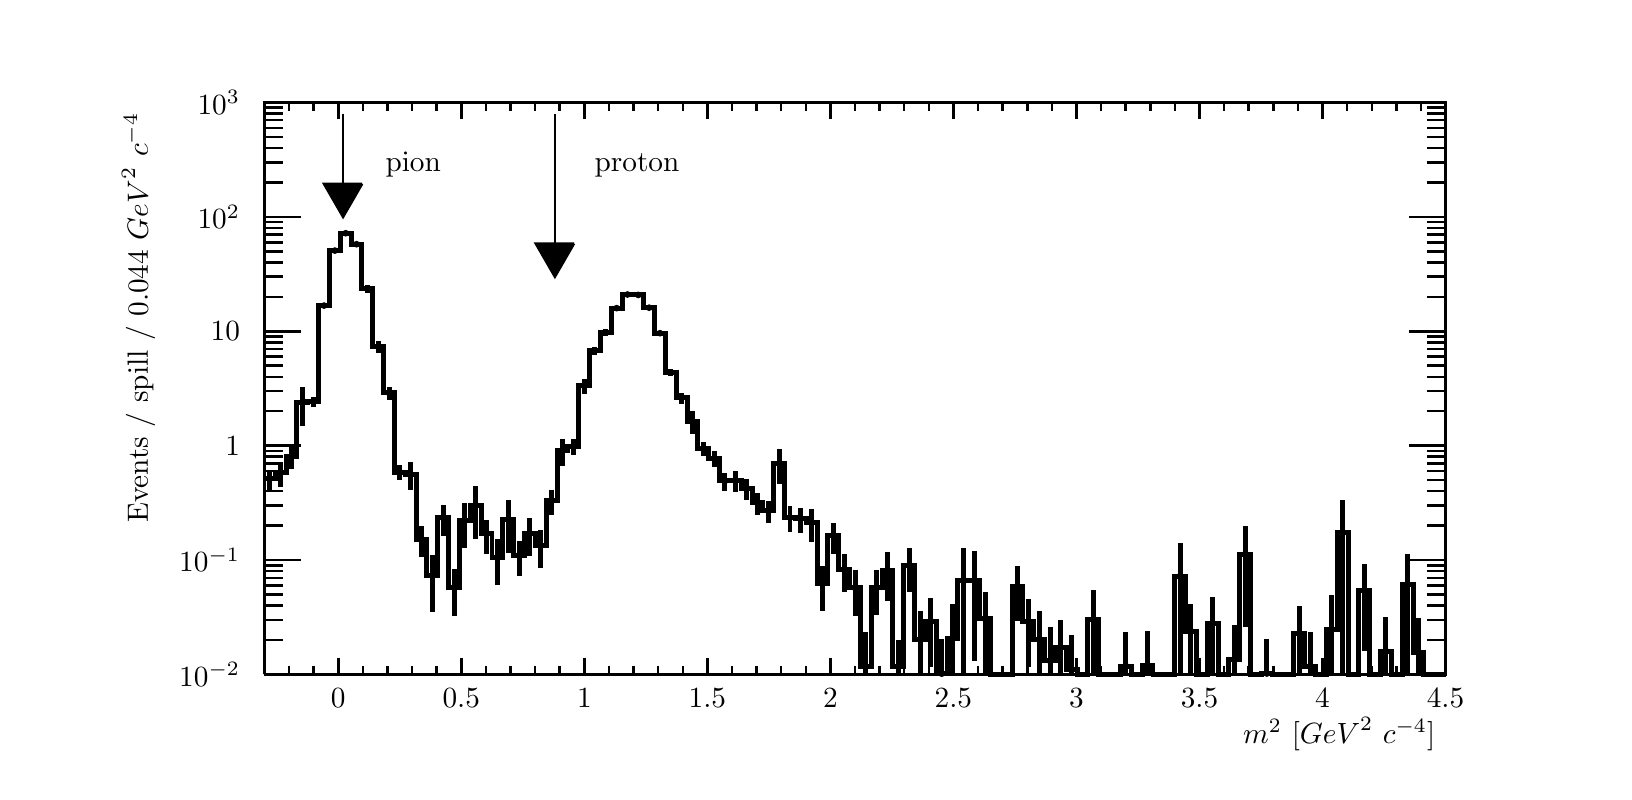
\begin{tikzpicture}
\pgfdeclareplotmark{cross} {
\pgfpathmoveto{\pgfpoint{-0.3\pgfplotmarksize}{\pgfplotmarksize}}
\pgfpathlineto{\pgfpoint{+0.3\pgfplotmarksize}{\pgfplotmarksize}}
\pgfpathlineto{\pgfpoint{+0.3\pgfplotmarksize}{0.3\pgfplotmarksize}}
\pgfpathlineto{\pgfpoint{+1\pgfplotmarksize}{0.3\pgfplotmarksize}}
\pgfpathlineto{\pgfpoint{+1\pgfplotmarksize}{-0.3\pgfplotmarksize}}
\pgfpathlineto{\pgfpoint{+0.3\pgfplotmarksize}{-0.3\pgfplotmarksize}}
\pgfpathlineto{\pgfpoint{+0.3\pgfplotmarksize}{-1.\pgfplotmarksize}}
\pgfpathlineto{\pgfpoint{-0.3\pgfplotmarksize}{-1.\pgfplotmarksize}}
\pgfpathlineto{\pgfpoint{-0.3\pgfplotmarksize}{-0.3\pgfplotmarksize}}
\pgfpathlineto{\pgfpoint{-1.\pgfplotmarksize}{-0.3\pgfplotmarksize}}
\pgfpathlineto{\pgfpoint{-1.\pgfplotmarksize}{0.3\pgfplotmarksize}}
\pgfpathlineto{\pgfpoint{-0.3\pgfplotmarksize}{0.3\pgfplotmarksize}}
\pgfpathclose
\pgfusepathqstroke
}
\pgfdeclareplotmark{cross*} {
\pgfpathmoveto{\pgfpoint{-0.3\pgfplotmarksize}{\pgfplotmarksize}}
\pgfpathlineto{\pgfpoint{+0.3\pgfplotmarksize}{\pgfplotmarksize}}
\pgfpathlineto{\pgfpoint{+0.3\pgfplotmarksize}{0.3\pgfplotmarksize}}
\pgfpathlineto{\pgfpoint{+1\pgfplotmarksize}{0.3\pgfplotmarksize}}
\pgfpathlineto{\pgfpoint{+1\pgfplotmarksize}{-0.3\pgfplotmarksize}}
\pgfpathlineto{\pgfpoint{+0.3\pgfplotmarksize}{-0.3\pgfplotmarksize}}
\pgfpathlineto{\pgfpoint{+0.3\pgfplotmarksize}{-1.\pgfplotmarksize}}
\pgfpathlineto{\pgfpoint{-0.3\pgfplotmarksize}{-1.\pgfplotmarksize}}
\pgfpathlineto{\pgfpoint{-0.3\pgfplotmarksize}{-0.3\pgfplotmarksize}}
\pgfpathlineto{\pgfpoint{-1.\pgfplotmarksize}{-0.3\pgfplotmarksize}}
\pgfpathlineto{\pgfpoint{-1.\pgfplotmarksize}{0.3\pgfplotmarksize}}
\pgfpathlineto{\pgfpoint{-0.3\pgfplotmarksize}{0.3\pgfplotmarksize}}
\pgfpathclose
\pgfusepathqfillstroke
}
\pgfdeclareplotmark{newstar} {
\pgfpathmoveto{\pgfqpoint{0pt}{\pgfplotmarksize}}
\pgfpathlineto{\pgfqpointpolar{44}{0.5\pgfplotmarksize}}
\pgfpathlineto{\pgfqpointpolar{18}{\pgfplotmarksize}}
\pgfpathlineto{\pgfqpointpolar{-20}{0.5\pgfplotmarksize}}
\pgfpathlineto{\pgfqpointpolar{-54}{\pgfplotmarksize}}
\pgfpathlineto{\pgfqpointpolar{-90}{0.5\pgfplotmarksize}}
\pgfpathlineto{\pgfqpointpolar{234}{\pgfplotmarksize}}
\pgfpathlineto{\pgfqpointpolar{198}{0.5\pgfplotmarksize}}
\pgfpathlineto{\pgfqpointpolar{162}{\pgfplotmarksize}}
\pgfpathlineto{\pgfqpointpolar{134}{0.5\pgfplotmarksize}}
\pgfpathclose
\pgfusepathqstroke
}
\pgfdeclareplotmark{newstar*} {
\pgfpathmoveto{\pgfqpoint{0pt}{\pgfplotmarksize}}
\pgfpathlineto{\pgfqpointpolar{44}{0.5\pgfplotmarksize}}
\pgfpathlineto{\pgfqpointpolar{18}{\pgfplotmarksize}}
\pgfpathlineto{\pgfqpointpolar{-20}{0.5\pgfplotmarksize}}
\pgfpathlineto{\pgfqpointpolar{-54}{\pgfplotmarksize}}
\pgfpathlineto{\pgfqpointpolar{-90}{0.5\pgfplotmarksize}}
\pgfpathlineto{\pgfqpointpolar{234}{\pgfplotmarksize}}
\pgfpathlineto{\pgfqpointpolar{198}{0.5\pgfplotmarksize}}
\pgfpathlineto{\pgfqpointpolar{162}{\pgfplotmarksize}}
\pgfpathlineto{\pgfqpointpolar{134}{0.5\pgfplotmarksize}}
\pgfpathclose
\pgfusepathqfillstroke
}
\definecolor{c}{rgb}{1,1,1};
\draw [color=c, fill=c] (0,0) rectangle (20,9.43311);
\draw [color=c, fill=c] (3,1.2263) rectangle (18,8.4898);
\definecolor{c}{rgb}{0,0,0};
\draw [c,line width=0.9] (3,1.2263) -- (3,8.4898) -- (18,8.4898) -- (18,1.2263) -- (3,1.2263);
\definecolor{c}{rgb}{1,1,1};
\draw [color=c, fill=c] (3,1.2263) rectangle (18,8.4898);
\definecolor{c}{rgb}{0,0,0};
\draw [c,line width=0.9] (3,1.2263) -- (3,8.4898) -- (18,8.4898) -- (18,1.2263) -- (3,1.2263);
\draw [c,line width=1.8] (3.06881,3.56872) -- (3.06881,3.71136);
\draw [c,line width=1.8] (3.06881,3.71136) -- (3.06881,3.82762);
\foreach \P in {(3.06881,3.71136)}{\draw[mark options={color=c,fill=c},mark size=2.402402pt,mark=*,mark size=1pt] plot coordinates {\P};}
\draw [c,line width=1.8] (3.20642,3.60405) -- (3.20642,3.78774);
\draw [c,line width=1.8] (3.20642,3.78774) -- (3.20642,3.92983);
\foreach \P in {(3.20642,3.78774)}{\draw[mark options={color=c,fill=c},mark size=2.402402pt,mark=*,mark size=1pt] plot coordinates {\P};}
\draw [c,line width=1.8] (3.34404,3.83272) -- (3.34404,3.99102);
\draw [c,line width=1.8] (3.34404,3.99102) -- (3.34404,4.11746);
\foreach \P in {(3.34404,3.99102)}{\draw[mark options={color=c,fill=c},mark size=2.402402pt,mark=*,mark size=1pt] plot coordinates {\P};}
\draw [c,line width=1.8] (3.48165,4.37763) -- (3.48165,4.6782);
\draw [c,line width=1.8] (3.48165,4.6782) -- (3.48165,4.88094);
\foreach \P in {(3.48165,4.6782)}{\draw[mark options={color=c,fill=c},mark size=2.402402pt,mark=*,mark size=1pt] plot coordinates {\P};}
\draw [c,line width=1.8] (3.61927,4.62245) -- (3.61927,4.6917);
\draw [c,line width=1.8] (3.61927,4.6917) -- (3.61927,4.7541);
\foreach \P in {(3.61927,4.6917)}{\draw[mark options={color=c,fill=c},mark size=2.402402pt,mark=*,mark size=1pt] plot coordinates {\P};}
\draw [c,line width=1.8] (3.75688,5.88089) -- (3.75688,5.91059);
\draw [c,line width=1.8] (3.75688,5.91059) -- (3.75688,5.93895);
\foreach \P in {(3.75688,5.91059)}{\draw[mark options={color=c,fill=c},mark size=2.402402pt,mark=*,mark size=1pt] plot coordinates {\P};}
\draw [c,line width=1.8] (3.8945,6.58821) -- (3.8945,6.609);
\draw [c,line width=1.8] (3.8945,6.609) -- (3.8945,6.62913);
\foreach \P in {(3.8945,6.609)}{\draw[mark options={color=c,fill=c},mark size=2.402402pt,mark=*,mark size=1pt] plot coordinates {\P};}
\draw [c,line width=1.8] (4.03211,6.80875) -- (4.03211,6.8294);
\draw [c,line width=1.8] (4.03211,6.8294) -- (4.03211,6.8494);
\foreach \P in {(4.03211,6.8294)}{\draw[mark options={color=c,fill=c},mark size=2.402402pt,mark=*,mark size=1pt] plot coordinates {\P};}
\draw [c,line width=1.8] (4.16972,6.66216) -- (4.16972,6.68997);
\draw [c,line width=1.8] (4.16972,6.68997) -- (4.16972,6.7166);
\foreach \P in {(4.16972,6.68997)}{\draw[mark options={color=c,fill=c},mark size=2.402402pt,mark=*,mark size=1pt] plot coordinates {\P};}
\draw [c,line width=1.8] (4.30734,6.07616) -- (4.30734,6.12807);
\draw [c,line width=1.8] (4.30734,6.12807) -- (4.30734,6.17604);
\foreach \P in {(4.30734,6.12807)}{\draw[mark options={color=c,fill=c},mark size=2.402402pt,mark=*,mark size=1pt] plot coordinates {\P};}
\draw [c,line width=1.8] (4.44495,5.31081) -- (4.44495,5.39135);
\draw [c,line width=1.8] (4.44495,5.39135) -- (4.44495,5.46277);
\foreach \P in {(4.44495,5.39135)}{\draw[mark options={color=c,fill=c},mark size=2.402402pt,mark=*,mark size=1pt] plot coordinates {\P};}
\draw [c,line width=1.8] (4.58257,4.71441) -- (4.58257,4.80088);
\draw [c,line width=1.8] (4.58257,4.80088) -- (4.58257,4.87692);
\foreach \P in {(4.58257,4.80088)}{\draw[mark options={color=c,fill=c},mark size=2.402402pt,mark=*,mark size=1pt] plot coordinates {\P};}
\draw [c,line width=1.8] (4.72018,3.69222) -- (4.72018,3.794);
\draw [c,line width=1.8] (4.72018,3.794) -- (4.72018,3.88161);
\foreach \P in {(4.72018,3.794)}{\draw[mark options={color=c,fill=c},mark size=2.402402pt,mark=*,mark size=1pt] plot coordinates {\P};}
\draw [c,line width=1.8] (4.8578,3.56322) -- (4.8578,3.7652);
\draw [c,line width=1.8] (4.8578,3.7652) -- (4.8578,3.91796);
\foreach \P in {(4.8578,3.7652)}{\draw[mark options={color=c,fill=c},mark size=2.402402pt,mark=*,mark size=1pt] plot coordinates {\P};}
\draw [c,line width=1.8] (4.99541,2.72369) -- (4.99541,2.944);
\draw [c,line width=1.8] (4.99541,2.944) -- (4.99541,3.10698);
\foreach \P in {(4.99541,2.944)}{\draw[mark options={color=c,fill=c},mark size=2.402402pt,mark=*,mark size=1pt] plot coordinates {\P};}
\draw [c,line width=1.8] (5.13303,2.02126) -- (5.13303,2.48397);
\draw [c,line width=1.8] (5.13303,2.48397) -- (5.13303,2.74802);
\foreach \P in {(5.13303,2.48397)}{\draw[mark options={color=c,fill=c},mark size=2.402402pt,mark=*,mark size=1pt] plot coordinates {\P};}
\draw [c,line width=1.8] (5.27064,2.98961) -- (5.27064,3.21415);
\draw [c,line width=1.8] (5.27064,3.21415) -- (5.27064,3.37941);
\foreach \P in {(5.27064,3.21415)}{\draw[mark options={color=c,fill=c},mark size=2.402402pt,mark=*,mark size=1pt] plot coordinates {\P};}
\draw [c,line width=1.8] (5.40826,1.96462) -- (5.40826,2.33111);
\draw [c,line width=1.8] (5.40826,2.33111) -- (5.40826,2.56143);
\foreach \P in {(5.40826,2.33111)}{\draw[mark options={color=c,fill=c},mark size=2.402402pt,mark=*,mark size=1pt] plot coordinates {\P};}
\draw [c,line width=1.8] (5.54587,2.82628) -- (5.54587,3.17889);
\draw [c,line width=1.8] (5.54587,3.17889) -- (5.54587,3.40373);
\foreach \P in {(5.54587,3.17889)}{\draw[mark options={color=c,fill=c},mark size=2.402402pt,mark=*,mark size=1pt] plot coordinates {\P};}
\draw [c,line width=1.8] (5.68349,2.95178) -- (5.68349,3.37453);
\draw [c,line width=1.8] (5.68349,3.37453) -- (5.68349,3.62542);
\foreach \P in {(5.68349,3.37453)}{\draw[mark options={color=c,fill=c},mark size=2.402402pt,mark=*,mark size=1pt] plot coordinates {\P};}
\draw [c,line width=1.8] (5.8211,2.75545) -- (5.8211,3.01109);
\draw [c,line width=1.8] (5.8211,3.01109) -- (5.8211,3.19251);
\foreach \P in {(5.8211,3.01109)}{\draw[mark options={color=c,fill=c},mark size=2.402402pt,mark=*,mark size=1pt] plot coordinates {\P};}
\draw [c,line width=1.8] (5.95872,2.3592) -- (5.95872,2.71711);
\draw [c,line width=1.8] (5.95872,2.71711) -- (5.95872,2.94407);
\foreach \P in {(5.95872,2.71711)}{\draw[mark options={color=c,fill=c},mark size=2.402402pt,mark=*,mark size=1pt] plot coordinates {\P};}
\draw [c,line width=1.8] (6.09633,2.76628) -- (6.09633,3.19469);
\draw [c,line width=1.8] (6.09633,3.19469) -- (6.09633,3.4475);
\foreach \P in {(6.09633,3.19469)}{\draw[mark options={color=c,fill=c},mark size=2.402402pt,mark=*,mark size=1pt] plot coordinates {\P};}
\draw [c,line width=1.8] (6.23394,2.47429) -- (6.23394,2.73953);
\draw [c,line width=1.8] (6.23394,2.73953) -- (6.23394,2.92569);
\foreach \P in {(6.23394,2.73953)}{\draw[mark options={color=c,fill=c},mark size=2.402402pt,mark=*,mark size=1pt] plot coordinates {\P};}
\draw [c,line width=1.8] (6.37156,2.73579) -- (6.37156,3.01506);
\draw [c,line width=1.8] (6.37156,3.01506) -- (6.37156,3.20796);
\foreach \P in {(6.37156,3.01506)}{\draw[mark options={color=c,fill=c},mark size=2.402402pt,mark=*,mark size=1pt] plot coordinates {\P};}
\draw [c,line width=1.8] (6.50917,2.57445) -- (6.50917,2.86253);
\draw [c,line width=1.8] (6.50917,2.86253) -- (6.50917,3.05956);
\foreach \P in {(6.50917,2.86253)}{\draw[mark options={color=c,fill=c},mark size=2.402402pt,mark=*,mark size=1pt] plot coordinates {\P};}
\draw [c,line width=1.8] (6.64679,3.25685) -- (6.64679,3.42962);
\draw [c,line width=1.8] (6.64679,3.42962) -- (6.64679,3.56511);
\foreach \P in {(6.64679,3.42962)}{\draw[mark options={color=c,fill=c},mark size=2.402402pt,mark=*,mark size=1pt] plot coordinates {\P};}
\draw [c,line width=1.8] (6.7844,3.87258) -- (6.7844,4.06998);
\draw [c,line width=1.8] (6.7844,4.06998) -- (6.7844,4.22011);
\foreach \P in {(6.7844,4.06998)}{\draw[mark options={color=c,fill=c},mark size=2.402402pt,mark=*,mark size=1pt] plot coordinates {\P};}
\draw [c,line width=1.8] (6.92202,4.0118) -- (6.92202,4.12585);
\draw [c,line width=1.8] (6.92202,4.12585) -- (6.92202,4.22241);
\foreach \P in {(6.92202,4.12585)}{\draw[mark options={color=c,fill=c},mark size=2.402402pt,mark=*,mark size=1pt] plot coordinates {\P};}
\draw [c,line width=1.8] (7.05963,4.78915) -- (7.05963,4.89028);
\draw [c,line width=1.8] (7.05963,4.89028) -- (7.05963,4.97742);
\foreach \P in {(7.05963,4.89028)}{\draw[mark options={color=c,fill=c},mark size=2.402402pt,mark=*,mark size=1pt] plot coordinates {\P};}
\draw [c,line width=1.8] (7.19725,5.28396) -- (7.19725,5.33785);
\draw [c,line width=1.8] (7.19725,5.33785) -- (7.19725,5.3875);
\foreach \P in {(7.19725,5.33785)}{\draw[mark options={color=c,fill=c},mark size=2.402402pt,mark=*,mark size=1pt] plot coordinates {\P};}
\draw [c,line width=1.8] (7.33486,5.52386) -- (7.33486,5.57101);
\draw [c,line width=1.8] (7.33486,5.57101) -- (7.33486,5.61488);
\foreach \P in {(7.33486,5.57101)}{\draw[mark options={color=c,fill=c},mark size=2.402402pt,mark=*,mark size=1pt] plot coordinates {\P};}
\draw [c,line width=1.8] (7.47248,5.84918) -- (7.47248,5.87775);
\draw [c,line width=1.8] (7.47248,5.87775) -- (7.47248,5.90507);
\foreach \P in {(7.47248,5.87775)}{\draw[mark options={color=c,fill=c},mark size=2.402402pt,mark=*,mark size=1pt] plot coordinates {\P};}
\draw [c,line width=1.8] (7.61009,6.02421) -- (7.61009,6.05102);
\draw [c,line width=1.8] (7.61009,6.05102) -- (7.61009,6.07674);
\foreach \P in {(7.61009,6.05102)}{\draw[mark options={color=c,fill=c},mark size=2.402402pt,mark=*,mark size=1pt] plot coordinates {\P};}
\draw [c,line width=1.8] (7.74771,6.02286) -- (7.74771,6.046);
\draw [c,line width=1.8] (7.74771,6.046) -- (7.74771,6.06832);
\foreach \P in {(7.74771,6.046)}{\draw[mark options={color=c,fill=c},mark size=2.402402pt,mark=*,mark size=1pt] plot coordinates {\P};}
\draw [c,line width=1.8] (7.88532,5.85613) -- (7.88532,5.8838);
\draw [c,line width=1.8] (7.88532,5.8838) -- (7.88532,5.91031);
\foreach \P in {(7.88532,5.8838)}{\draw[mark options={color=c,fill=c},mark size=2.402402pt,mark=*,mark size=1pt] plot coordinates {\P};}
\draw [c,line width=1.8] (8.02294,5.52535) -- (8.02294,5.56009);
\draw [c,line width=1.8] (8.02294,5.56009) -- (8.02294,5.59301);
\foreach \P in {(8.02294,5.56009)}{\draw[mark options={color=c,fill=c},mark size=2.402402pt,mark=*,mark size=1pt] plot coordinates {\P};}
\draw [c,line width=1.8] (8.16055,5.01206) -- (8.16055,5.0609);
\draw [c,line width=1.8] (8.16055,5.0609) -- (8.16055,5.10624);
\foreach \P in {(8.16055,5.0609)}{\draw[mark options={color=c,fill=c},mark size=2.402402pt,mark=*,mark size=1pt] plot coordinates {\P};}
\draw [c,line width=1.8] (8.29817,4.66691) -- (8.29817,4.73945);
\draw [c,line width=1.8] (8.29817,4.73945) -- (8.29817,4.80449);
\foreach \P in {(8.29817,4.73945)}{\draw[mark options={color=c,fill=c},mark size=2.402402pt,mark=*,mark size=1pt] plot coordinates {\P};}
\draw [c,line width=1.8] (8.43578,4.28359) -- (8.43578,4.44033);
\draw [c,line width=1.8] (8.43578,4.44033) -- (8.43578,4.56577);
\foreach \P in {(8.43578,4.44033)}{\draw[mark options={color=c,fill=c},mark size=2.402402pt,mark=*,mark size=1pt] plot coordinates {\P};}
\draw [c,line width=1.8] (8.57339,3.99655) -- (8.57339,4.09149);
\draw [c,line width=1.8] (8.57339,4.09149) -- (8.57339,4.174);
\foreach \P in {(8.57339,4.09149)}{\draw[mark options={color=c,fill=c},mark size=2.402402pt,mark=*,mark size=1pt] plot coordinates {\P};}
\draw [c,line width=1.8] (8.71101,3.85907) -- (8.71101,3.96865);
\draw [c,line width=1.8] (8.71101,3.96865) -- (8.71101,4.06199);
\foreach \P in {(8.71101,3.96865)}{\draw[mark options={color=c,fill=c},mark size=2.402402pt,mark=*,mark size=1pt] plot coordinates {\P};}
\draw [c,line width=1.8] (8.84862,3.56063) -- (8.84862,3.68393);
\draw [c,line width=1.8] (8.84862,3.68393) -- (8.84862,3.78703);
\foreach \P in {(8.84862,3.68393)}{\draw[mark options={color=c,fill=c},mark size=2.402402pt,mark=*,mark size=1pt] plot coordinates {\P};}
\draw [c,line width=1.8] (8.98624,3.54614) -- (8.98624,3.69032);
\draw [c,line width=1.8] (8.98624,3.69032) -- (8.98624,3.8076);
\foreach \P in {(8.98624,3.69032)}{\draw[mark options={color=c,fill=c},mark size=2.402402pt,mark=*,mark size=1pt] plot coordinates {\P};}
\draw [c,line width=1.8] (9.12385,3.44504) -- (9.12385,3.58819);
\draw [c,line width=1.8] (9.12385,3.58819) -- (9.12385,3.70479);
\foreach \P in {(9.12385,3.58819)}{\draw[mark options={color=c,fill=c},mark size=2.402402pt,mark=*,mark size=1pt] plot coordinates {\P};}
\draw [c,line width=1.8] (9.26147,3.2554) -- (9.26147,3.41055);
\draw [c,line width=1.8] (9.26147,3.41055) -- (9.26147,3.53499);
\foreach \P in {(9.26147,3.41055)}{\draw[mark options={color=c,fill=c},mark size=2.402402pt,mark=*,mark size=1pt] plot coordinates {\P};}
\draw [c,line width=1.8] (9.39908,3.14598) -- (9.39908,3.30399);
\draw [c,line width=1.8] (9.39908,3.30399) -- (9.39908,3.43025);
\foreach \P in {(9.39908,3.30399)}{\draw[mark options={color=c,fill=c},mark size=2.402402pt,mark=*,mark size=1pt] plot coordinates {\P};}
\draw [c,line width=1.8] (9.5367,3.64807) -- (9.5367,3.90256);
\draw [c,line width=1.8] (9.5367,3.90256) -- (9.5367,4.0834);
\foreach \P in {(9.5367,3.90256)}{\draw[mark options={color=c,fill=c},mark size=2.402402pt,mark=*,mark size=1pt] plot coordinates {\P};}
\draw [c,line width=1.8] (9.67431,3.03567) -- (9.67431,3.21987);
\draw [c,line width=1.8] (9.67431,3.21987) -- (9.67431,3.36227);
\foreach \P in {(9.67431,3.21987)}{\draw[mark options={color=c,fill=c},mark size=2.402402pt,mark=*,mark size=1pt] plot coordinates {\P};}
\draw [c,line width=1.8] (9.81193,3.02432) -- (9.81193,3.2043);
\draw [c,line width=1.8] (9.81193,3.2043) -- (9.81193,3.34417);
\foreach \P in {(9.81193,3.2043)}{\draw[mark options={color=c,fill=c},mark size=2.402402pt,mark=*,mark size=1pt] plot coordinates {\P};}
\draw [c,line width=1.8] (9.94954,2.90575) -- (9.94954,3.15507);
\draw [c,line width=1.8] (9.94954,3.15507) -- (9.94954,3.33329);
\foreach \P in {(9.94954,3.15507)}{\draw[mark options={color=c,fill=c},mark size=2.402402pt,mark=*,mark size=1pt] plot coordinates {\P};}
\draw [c,line width=1.8] (10.0872,2.03789) -- (10.0872,2.38235);
\draw [c,line width=1.8] (10.0872,2.38235) -- (10.0872,2.6039);
\foreach \P in {(10.0872,2.38235)}{\draw[mark options={color=c,fill=c},mark size=2.402402pt,mark=*,mark size=1pt] plot coordinates {\P};}
\draw [c,line width=1.8] (10.2248,2.75862) -- (10.2248,2.98477);
\draw [c,line width=1.8] (10.2248,2.98477) -- (10.2248,3.1509);
\foreach \P in {(10.2248,2.98477)}{\draw[mark options={color=c,fill=c},mark size=2.402402pt,mark=*,mark size=1pt] plot coordinates {\P};}
\draw [c,line width=1.8] (10.3624,2.27162) -- (10.3624,2.5586);
\draw [c,line width=1.8] (10.3624,2.5586) -- (10.3624,2.75512);
\foreach \P in {(10.3624,2.5586)}{\draw[mark options={color=c,fill=c},mark size=2.402402pt,mark=*,mark size=1pt] plot coordinates {\P};}
\draw [c,line width=1.8] (10.5,1.96858) -- (10.5,2.32496);
\draw [c,line width=1.8] (10.5,2.32496) -- (10.5,2.55131);
\foreach \P in {(10.5,2.32496)}{\draw[mark options={color=c,fill=c},mark size=2.402402pt,mark=*,mark size=1pt] plot coordinates {\P};}
\draw [c,line width=1.8] (10.6376,1.2263) -- (10.6376,1.3277);
\draw [c,line width=1.8] (10.6376,1.3277) -- (10.6376,1.76537);
\foreach \P in {(10.6376,1.3277)}{\draw[mark options={color=c,fill=c},mark size=2.402402pt,mark=*,mark size=1pt] plot coordinates {\P};}
\draw [c,line width=1.8] (10.7752,1.98377) -- (10.7752,2.32996);
\draw [c,line width=1.8] (10.7752,2.32996) -- (10.7752,2.55221);
\foreach \P in {(10.7752,2.32996)}{\draw[mark options={color=c,fill=c},mark size=2.402402pt,mark=*,mark size=1pt] plot coordinates {\P};}
\draw [c,line width=1.8] (10.9128,2.15956) -- (10.9128,2.54358);
\draw [c,line width=1.8] (10.9128,2.54358) -- (10.9128,2.78057);
\foreach \P in {(10.9128,2.54358)}{\draw[mark options={color=c,fill=c},mark size=2.402402pt,mark=*,mark size=1pt] plot coordinates {\P};}
\draw [c,line width=1.8] (11.0505,1.2263) -- (11.0505,1.32725);
\draw [c,line width=1.8] (11.0505,1.32725) -- (11.0505,1.6654);
\foreach \P in {(11.0505,1.32725)}{\draw[mark options={color=c,fill=c},mark size=2.402402pt,mark=*,mark size=1pt] plot coordinates {\P};}
\draw [c,line width=1.8] (11.1881,2.27742) -- (11.1881,2.61114);
\draw [c,line width=1.8] (11.1881,2.61114) -- (11.1881,2.82825);
\foreach \P in {(11.1881,2.61114)}{\draw[mark options={color=c,fill=c},mark size=2.402402pt,mark=*,mark size=1pt] plot coordinates {\P};}
\draw [c,line width=1.8] (11.3257,1.2263) -- (11.3257,1.67205);
\draw [c,line width=1.8] (11.3257,1.67205) -- (11.3257,2.03101);
\foreach \P in {(11.3257,1.67205)}{\draw[mark options={color=c,fill=c},mark size=2.402402pt,mark=*,mark size=1pt] plot coordinates {\P};}
\draw [c,line width=1.8] (11.4633,1.32341) -- (11.4633,1.90285);
\draw [c,line width=1.8] (11.4633,1.90285) -- (11.4633,2.19972);
\foreach \P in {(11.4633,1.90285)}{\draw[mark options={color=c,fill=c},mark size=2.402402pt,mark=*,mark size=1pt] plot coordinates {\P};}
\draw [c,line width=1.8] (11.6009,1.2263) -- (11.6009,1.23591);
\draw [c,line width=1.8] (11.6009,1.23591) -- (11.6009,1.67363);
\foreach \P in {(11.6009,1.23591)}{\draw[mark options={color=c,fill=c},mark size=2.402402pt,mark=*,mark size=1pt] plot coordinates {\P};}
\draw [c,line width=1.8] (11.7385,1.2263) -- (11.7385,1.68607);
\draw [c,line width=1.8] (11.7385,1.68607) -- (11.7385,2.12389);
\foreach \P in {(11.7385,1.68607)}{\draw[mark options={color=c,fill=c},mark size=2.402402pt,mark=*,mark size=1pt] plot coordinates {\P};}
\draw [c,line width=1.8] (11.8761,1.2263) -- (11.8761,2.4233);
\draw [c,line width=1.8] (11.8761,2.4233) -- (11.8761,2.834);
\foreach \P in {(11.8761,2.4233)}{\draw[mark options={color=c,fill=c},mark size=2.402402pt,mark=*,mark size=1pt] plot coordinates {\P};}
\draw [c,line width=1.8] (12.0138,1.39728) -- (12.0138,2.4205);
\draw [c,line width=1.8] (12.0138,2.4205) -- (12.0138,2.79219);
\foreach \P in {(12.0138,2.4205)}{\draw[mark options={color=c,fill=c},mark size=2.402402pt,mark=*,mark size=1pt] plot coordinates {\P};}
\draw [c,line width=1.8] (12.1514,1.2263) -- (12.1514,1.93107);
\draw [c,line width=1.8] (12.1514,1.93107) -- (12.1514,2.27464);
\foreach \P in {(12.1514,1.93107)}{\draw[mark options={color=c,fill=c},mark size=2.402402pt,mark=*,mark size=1pt] plot coordinates {\P};}
\draw [c,line width=1.8] (12.5642,1.90555) -- (12.5642,2.34491);
\draw [c,line width=1.8] (12.5642,2.34491) -- (12.5642,2.60141);
\foreach \P in {(12.5642,2.34491)}{\draw[mark options={color=c,fill=c},mark size=2.402402pt,mark=*,mark size=1pt] plot coordinates {\P};}
\draw [c,line width=1.8] (12.7018,1.31527) -- (12.7018,1.89266);
\draw [c,line width=1.8] (12.7018,1.89266) -- (12.7018,2.18901);
\foreach \P in {(12.7018,1.89266)}{\draw[mark options={color=c,fill=c},mark size=2.402402pt,mark=*,mark size=1pt] plot coordinates {\P};}
\draw [c,line width=1.8] (12.8394,1.2263) -- (12.8394,1.6727);
\draw [c,line width=1.8] (12.8394,1.6727) -- (12.8394,2.03107);
\foreach \P in {(12.8394,1.6727)}{\draw[mark options={color=c,fill=c},mark size=2.402402pt,mark=*,mark size=1pt] plot coordinates {\P};}
\draw [c,line width=1.8] (12.9771,1.2263) -- (12.9771,1.39712);
\draw [c,line width=1.8] (12.9771,1.39712) -- (12.9771,1.83482);
\foreach \P in {(12.9771,1.39712)}{\draw[mark options={color=c,fill=c},mark size=2.402402pt,mark=*,mark size=1pt] plot coordinates {\P};}
\draw [c,line width=1.8] (13.1147,1.2263) -- (13.1147,1.5685);
\draw [c,line width=1.8] (13.1147,1.5685) -- (13.1147,1.9191);
\foreach \P in {(13.1147,1.5685)}{\draw[mark options={color=c,fill=c},mark size=2.402402pt,mark=*,mark size=1pt] plot coordinates {\P};}
\draw [c,line width=1.8] (13.2523,1.2263) -- (13.2523,1.2852);
\draw [c,line width=1.8] (13.2523,1.2852) -- (13.2523,1.72288);
\foreach \P in {(13.2523,1.2852)}{\draw[mark options={color=c,fill=c},mark size=2.402402pt,mark=*,mark size=1pt] plot coordinates {\P};}
\draw [c,line width=1.8] (13.5275,1.2263) -- (13.5275,1.92356);
\draw [c,line width=1.8] (13.5275,1.92356) -- (13.5275,2.30434);
\foreach \P in {(13.5275,1.92356)}{\draw[mark options={color=c,fill=c},mark size=2.402402pt,mark=*,mark size=1pt] plot coordinates {\P};}
\draw [c,line width=1.8] (13.9404,1.2263) -- (13.9404,1.33199);
\draw [c,line width=1.8] (13.9404,1.33199) -- (13.9404,1.76967);
\foreach \P in {(13.9404,1.33199)}{\draw[mark options={color=c,fill=c},mark size=2.402402pt,mark=*,mark size=1pt] plot coordinates {\P};}
\draw [c,line width=1.8] (14.2156,1.2263) -- (14.2156,1.34151);
\draw [c,line width=1.8] (14.2156,1.34151) -- (14.2156,1.77924);
\foreach \P in {(14.2156,1.34151)}{\draw[mark options={color=c,fill=c},mark size=2.402402pt,mark=*,mark size=1pt] plot coordinates {\P};}
\draw [c,line width=1.8] (14.6284,1.2263) -- (14.6284,2.47584);
\draw [c,line width=1.8] (14.6284,2.47584) -- (14.6284,2.88914);
\foreach \P in {(14.6284,2.47584)}{\draw[mark options={color=c,fill=c},mark size=2.402402pt,mark=*,mark size=1pt] plot coordinates {\P};}
\draw [c,line width=1.8] (14.7661,1.2263) -- (14.7661,1.77723);
\draw [c,line width=1.8] (14.7661,1.77723) -- (14.7661,2.11494);
\foreach \P in {(14.7661,1.77723)}{\draw[mark options={color=c,fill=c},mark size=2.402402pt,mark=*,mark size=1pt] plot coordinates {\P};}
\draw [c,line width=1.8] (15.0413,1.2263) -- (15.0413,1.86949);
\draw [c,line width=1.8] (15.0413,1.86949) -- (15.0413,2.21436);
\foreach \P in {(15.0413,1.86949)}{\draw[mark options={color=c,fill=c},mark size=2.402402pt,mark=*,mark size=1pt] plot coordinates {\P};}
\draw [c,line width=1.8] (15.3165,1.2263) -- (15.3165,1.41421);
\draw [c,line width=1.8] (15.3165,1.41421) -- (15.3165,1.85179);
\foreach \P in {(15.3165,1.41421)}{\draw[mark options={color=c,fill=c},mark size=2.402402pt,mark=*,mark size=1pt] plot coordinates {\P};}
\draw [c,line width=1.8] (15.4541,1.82819) -- (15.4541,2.75279);
\draw [c,line width=1.8] (15.4541,2.75279) -- (15.4541,3.11268);
\foreach \P in {(15.4541,2.75279)}{\draw[mark options={color=c,fill=c},mark size=2.402402pt,mark=*,mark size=1pt] plot coordinates {\P};}
\draw [c,line width=1.8] (15.7294,1.2263) -- (15.7294,1.23755);
\draw [c,line width=1.8] (15.7294,1.23755) -- (15.7294,1.67527);
\foreach \P in {(15.7294,1.23755)}{\draw[mark options={color=c,fill=c},mark size=2.402402pt,mark=*,mark size=1pt] plot coordinates {\P};}
\draw [c,line width=1.8] (16.1422,1.2263) -- (16.1422,1.75095);
\draw [c,line width=1.8] (16.1422,1.75095) -- (16.1422,2.09382);
\foreach \P in {(16.1422,1.75095)}{\draw[mark options={color=c,fill=c},mark size=2.402402pt,mark=*,mark size=1pt] plot coordinates {\P};}
\draw [c,line width=1.8] (16.2798,1.2263) -- (16.2798,1.33171);
\draw [c,line width=1.8] (16.2798,1.33171) -- (16.2798,1.76939);
\foreach \P in {(16.2798,1.33171)}{\draw[mark options={color=c,fill=c},mark size=2.402402pt,mark=*,mark size=1pt] plot coordinates {\P};}
\draw [c,line width=1.8] (16.555,1.2263) -- (16.555,1.7949);
\draw [c,line width=1.8] (16.555,1.7949) -- (16.555,2.23253);
\foreach \P in {(16.555,1.7949)}{\draw[mark options={color=c,fill=c},mark size=2.402402pt,mark=*,mark size=1pt] plot coordinates {\P};}
\draw [c,line width=1.8] (16.6927,1.2263) -- (16.6927,3.02411);
\draw [c,line width=1.8] (16.6927,3.02411) -- (16.6927,3.44421);
\foreach \P in {(16.6927,3.02411)}{\draw[mark options={color=c,fill=c},mark size=2.402402pt,mark=*,mark size=1pt] plot coordinates {\P};}
\draw [c,line width=1.8] (16.9679,1.52976) -- (16.9679,2.28801);
\draw [c,line width=1.8] (16.9679,2.28801) -- (16.9679,2.62255);
\foreach \P in {(16.9679,2.28801)}{\draw[mark options={color=c,fill=c},mark size=2.402402pt,mark=*,mark size=1pt] plot coordinates {\P};}
\draw [c,line width=1.8] (17.2431,1.2263) -- (17.2431,1.52343);
\draw [c,line width=1.8] (17.2431,1.52343) -- (17.2431,1.96114);
\foreach \P in {(17.2431,1.52343)}{\draw[mark options={color=c,fill=c},mark size=2.402402pt,mark=*,mark size=1pt] plot coordinates {\P};}
\draw [c,line width=1.8] (17.5183,1.24079) -- (17.5183,2.37168);
\draw [c,line width=1.8] (17.5183,2.37168) -- (17.5183,2.75413);
\foreach \P in {(17.5183,2.37168)}{\draw[mark options={color=c,fill=c},mark size=2.402402pt,mark=*,mark size=1pt] plot coordinates {\P};}
\draw [c,line width=1.8] (17.656,1.2263) -- (17.656,1.50107);
\draw [c,line width=1.8] (17.656,1.50107) -- (17.656,1.93861);
\foreach \P in {(17.656,1.50107)}{\draw[mark options={color=c,fill=c},mark size=2.402402pt,mark=*,mark size=1pt] plot coordinates {\P};}
\draw [c,line width=1.8] (3,3.71136) -- (3.13761,3.71136) -- (3.13761,3.78774) -- (3.27523,3.78774) -- (3.27523,3.99102) -- (3.41284,3.99102) -- (3.41284,4.6782) -- (3.55046,4.6782) -- (3.55046,4.6917) -- (3.68807,4.6917) -- (3.68807,5.91059) --
 (3.82569,5.91059) -- (3.82569,6.609) -- (3.9633,6.609) -- (3.9633,6.8294) -- (4.10092,6.8294) -- (4.10092,6.68997) -- (4.23853,6.68997) -- (4.23853,6.12807) -- (4.37615,6.12807) -- (4.37615,5.39135) -- (4.51376,5.39135) -- (4.51376,4.80088) --
 (4.65138,4.80088) -- (4.65138,3.794) -- (4.78899,3.794) -- (4.78899,3.7652) -- (4.92661,3.7652) -- (4.92661,2.944) -- (5.06422,2.944) -- (5.06422,2.48397) -- (5.20184,2.48397) -- (5.20184,3.21415) -- (5.33945,3.21415) -- (5.33945,2.33111) --
 (5.47706,2.33111) -- (5.47706,3.17889) -- (5.61468,3.17889) -- (5.61468,3.37453) -- (5.75229,3.37453) -- (5.75229,3.01109) -- (5.88991,3.01109) -- (5.88991,2.71711) -- (6.02752,2.71711) -- (6.02752,3.19469) -- (6.16514,3.19469) -- (6.16514,2.73953)
 -- (6.30275,2.73953) -- (6.30275,3.01506) -- (6.44037,3.01506) -- (6.44037,2.86253) -- (6.57798,2.86253) -- (6.57798,3.42962) -- (6.7156,3.42962) -- (6.7156,4.06998) -- (6.85321,4.06998) -- (6.85321,4.12585) -- (6.99083,4.12585) -- (6.99083,4.89028)
 -- (7.12844,4.89028) -- (7.12844,5.33785) -- (7.26606,5.33785) -- (7.26606,5.57101) -- (7.40367,5.57101) -- (7.40367,5.87775) -- (7.54128,5.87775) -- (7.54128,6.05102) -- (7.6789,6.05102) -- (7.6789,6.046) -- (7.81651,6.046) -- (7.81651,5.8838) --
 (7.95413,5.8838) -- (7.95413,5.56009) -- (8.09174,5.56009) -- (8.09174,5.0609) -- (8.22936,5.0609) -- (8.22936,4.73945) -- (8.36697,4.73945) -- (8.36697,4.44033) -- (8.50459,4.44033) -- (8.50459,4.09149) -- (8.6422,4.09149) -- (8.6422,3.96865) --
 (8.77982,3.96865) -- (8.77982,3.68393) -- (8.91743,3.68393) -- (8.91743,3.69032) -- (9.05505,3.69032) -- (9.05505,3.58819) -- (9.19266,3.58819) -- (9.19266,3.41055) -- (9.33028,3.41055) -- (9.33028,3.30399) -- (9.46789,3.30399) -- (9.46789,3.90256)
 -- (9.6055,3.90256) -- (9.6055,3.21987) -- (9.74312,3.21987) -- (9.74312,3.2043) -- (9.88073,3.2043) -- (9.88073,3.15507) -- (10.0183,3.15507) -- (10.0183,2.38235) -- (10.156,2.38235) -- (10.156,2.98477) -- (10.2936,2.98477) -- (10.2936,2.5586) --
 (10.4312,2.5586) -- (10.4312,2.32496) -- (10.5688,2.32496) -- (10.5688,1.3277) -- (10.7064,1.3277) -- (10.7064,2.32996) -- (10.844,2.32996) -- (10.844,2.54358) -- (10.9817,2.54358) -- (10.9817,1.32725) -- (11.1193,1.32725) -- (11.1193,2.61114) --
 (11.2569,2.61114) -- (11.2569,1.67205) -- (11.3945,1.67205) -- (11.3945,1.90285) -- (11.5321,1.90285) -- (11.5321,1.23591) -- (11.6697,1.23591) -- (11.6697,1.68607) -- (11.8073,1.68607) -- (11.8073,2.4233) -- (11.945,2.4233) -- (11.945,2.4205) --
 (12.0826,2.4205) -- (12.0826,1.93107) -- (12.2202,1.93107) -- (12.2202,1.2263) -- (12.3578,1.2263) -- (12.3578,1.2263) -- (12.4954,1.2263) -- (12.4954,2.34491) -- (12.633,2.34491) -- (12.633,1.89266) -- (12.7706,1.89266) -- (12.7706,1.6727) --
 (12.9083,1.6727) -- (12.9083,1.39712) -- (13.0459,1.39712) -- (13.0459,1.5685) -- (13.1835,1.5685) -- (13.1835,1.2852) -- (13.3211,1.2852) -- (13.3211,1.2263) -- (13.4587,1.2263) -- (13.4587,1.92356) -- (13.5963,1.92356) -- (13.5963,1.2263) --
 (13.7339,1.2263) -- (13.7339,1.2263) -- (13.8716,1.2263) -- (13.8716,1.33199) -- (14.0092,1.33199) -- (14.0092,1.2263) -- (14.1468,1.2263) -- (14.1468,1.34151) -- (14.2844,1.34151) -- (14.2844,1.2263) -- (14.422,1.2263) -- (14.422,1.2263) --
 (14.5596,1.2263) -- (14.5596,2.47584) -- (14.6972,2.47584) -- (14.6972,1.77723) -- (14.8349,1.77723) -- (14.8349,1.2263) -- (14.9725,1.2263) -- (14.9725,1.86949) -- (15.1101,1.86949) -- (15.1101,1.2263) -- (15.2477,1.2263) -- (15.2477,1.41421) --
 (15.3853,1.41421) -- (15.3853,2.75279) -- (15.5229,2.75279) -- (15.5229,1.2263) -- (15.6606,1.2263) -- (15.6606,1.23755) -- (15.7982,1.23755) -- (15.7982,1.2263) -- (15.9358,1.2263) -- (15.9358,1.2263) -- (16.0734,1.2263) -- (16.0734,1.75095) --
 (16.211,1.75095) -- (16.211,1.33171) -- (16.3486,1.33171) -- (16.3486,1.2263) -- (16.4862,1.2263) -- (16.4862,1.7949) -- (16.6239,1.7949) -- (16.6239,3.02411) -- (16.7615,3.02411) -- (16.7615,1.2263) -- (16.8991,1.2263) -- (16.8991,2.28801) --
 (17.0367,2.28801) -- (17.0367,1.2263) -- (17.1743,1.2263) -- (17.1743,1.52343) -- (17.3119,1.52343) -- (17.3119,1.2263) -- (17.4495,1.2263) -- (17.4495,2.37168) -- (17.5872,2.37168) -- (17.5872,1.50107) -- (17.7248,1.50107) -- (17.7248,1.2263) --
 (17.8624,1.2263) -- (17.8624,1.2263) -- (18,1.2263);
\draw [c,line width=0.9] (3,1.2263) -- (18,1.2263);
\draw [c,line width=0.9] (3.9375,1.43855) -- (3.9375,1.2263);
\draw [c,line width=0.9] (4.25,1.33243) -- (4.25,1.2263);
\draw [c,line width=0.9] (4.5625,1.33243) -- (4.5625,1.2263);
\draw [c,line width=0.9] (4.875,1.33243) -- (4.875,1.2263);
\draw [c,line width=0.9] (5.1875,1.33243) -- (5.1875,1.2263);
\draw [c,line width=0.9] (5.5,1.43855) -- (5.5,1.2263);
\draw [c,line width=0.9] (5.8125,1.33243) -- (5.8125,1.2263);
\draw [c,line width=0.9] (6.125,1.33243) -- (6.125,1.2263);
\draw [c,line width=0.9] (6.4375,1.33243) -- (6.4375,1.2263);
\draw [c,line width=0.9] (6.75,1.33243) -- (6.75,1.2263);
\draw [c,line width=0.9] (7.0625,1.43855) -- (7.0625,1.2263);
\draw [c,line width=0.9] (7.375,1.33243) -- (7.375,1.2263);
\draw [c,line width=0.9] (7.6875,1.33243) -- (7.6875,1.2263);
\draw [c,line width=0.9] (8,1.33243) -- (8,1.2263);
\draw [c,line width=0.9] (8.3125,1.33243) -- (8.3125,1.2263);
\draw [c,line width=0.9] (8.625,1.43855) -- (8.625,1.2263);
\draw [c,line width=0.9] (8.9375,1.33243) -- (8.9375,1.2263);
\draw [c,line width=0.9] (9.25,1.33243) -- (9.25,1.2263);
\draw [c,line width=0.9] (9.5625,1.33243) -- (9.5625,1.2263);
\draw [c,line width=0.9] (9.875,1.33243) -- (9.875,1.2263);
\draw [c,line width=0.9] (10.1875,1.43855) -- (10.1875,1.2263);
\draw [c,line width=0.9] (10.5,1.33243) -- (10.5,1.2263);
\draw [c,line width=0.9] (10.8125,1.33243) -- (10.8125,1.2263);
\draw [c,line width=0.9] (11.125,1.33243) -- (11.125,1.2263);
\draw [c,line width=0.9] (11.4375,1.33243) -- (11.4375,1.2263);
\draw [c,line width=0.9] (11.75,1.43855) -- (11.75,1.2263);
\draw [c,line width=0.9] (12.0625,1.33243) -- (12.0625,1.2263);
\draw [c,line width=0.9] (12.375,1.33243) -- (12.375,1.2263);
\draw [c,line width=0.9] (12.6875,1.33243) -- (12.6875,1.2263);
\draw [c,line width=0.9] (13,1.33243) -- (13,1.2263);
\draw [c,line width=0.9] (13.3125,1.43855) -- (13.3125,1.2263);
\draw [c,line width=0.9] (13.625,1.33243) -- (13.625,1.2263);
\draw [c,line width=0.9] (13.9375,1.33243) -- (13.9375,1.2263);
\draw [c,line width=0.9] (14.25,1.33243) -- (14.25,1.2263);
\draw [c,line width=0.9] (14.5625,1.33243) -- (14.5625,1.2263);
\draw [c,line width=0.9] (14.875,1.43855) -- (14.875,1.2263);
\draw [c,line width=0.9] (15.1875,1.33243) -- (15.1875,1.2263);
\draw [c,line width=0.9] (15.5,1.33243) -- (15.5,1.2263);
\draw [c,line width=0.9] (15.8125,1.33243) -- (15.8125,1.2263);
\draw [c,line width=0.9] (16.125,1.33243) -- (16.125,1.2263);
\draw [c,line width=0.9] (16.4375,1.43855) -- (16.4375,1.2263);
\draw [c,line width=0.9] (16.75,1.33243) -- (16.75,1.2263);
\draw [c,line width=0.9] (17.0625,1.33243) -- (17.0625,1.2263);
\draw [c,line width=0.9] (17.375,1.33243) -- (17.375,1.2263);
\draw [c,line width=0.9] (17.6875,1.33243) -- (17.6875,1.2263);
\draw [c,line width=0.9] (18,1.43855) -- (18,1.2263);
\draw [c,line width=0.9] (3.9375,1.43855) -- (3.9375,1.2263);
\draw [c,line width=0.9] (3.625,1.33243) -- (3.625,1.2263);
\draw [c,line width=0.9] (3.3125,1.33243) -- (3.3125,1.2263);
\draw [c,line width=0.9] (3,1.33243) -- (3,1.2263);
\draw [c,line width=0.9] (18,1.43855) -- (18,1.2263);
\draw [anchor=base] (3.9375,0.801814) node[scale=1.0576, color=c, rotate=0]{0};
\draw [anchor=base] (5.5,0.801814) node[scale=1.0576, color=c, rotate=0]{0.5};
\draw [anchor=base] (7.0625,0.801814) node[scale=1.0576, color=c, rotate=0]{1};
\draw [anchor=base] (8.625,0.801814) node[scale=1.0576, color=c, rotate=0]{1.5};
\draw [anchor=base] (10.1875,0.801814) node[scale=1.0576, color=c, rotate=0]{2};
\draw [anchor=base] (11.75,0.801814) node[scale=1.0576, color=c, rotate=0]{2.5};
\draw [anchor=base] (13.3125,0.801814) node[scale=1.0576, color=c, rotate=0]{3};
\draw [anchor=base] (14.875,0.801814) node[scale=1.0576, color=c, rotate=0]{3.5};
\draw [anchor=base] (16.4375,0.801814) node[scale=1.0576, color=c, rotate=0]{4};
\draw [anchor=base] (18,0.801814) node[scale=1.0576, color=c, rotate=0]{4.5};
\draw [anchor= east] (18,0.471655) node[scale=1.0576, color=c, rotate=0]{$m^{2}$ [$\text{GeV}^{2}~c^{-4}$]};
\draw [c,line width=0.9] (3,8.4898) -- (18,8.4898);
\draw [c,line width=0.9] (3.9375,8.27755) -- (3.9375,8.4898);
\draw [c,line width=0.9] (4.25,8.38367) -- (4.25,8.4898);
\draw [c,line width=0.9] (4.5625,8.38367) -- (4.5625,8.4898);
\draw [c,line width=0.9] (4.875,8.38367) -- (4.875,8.4898);
\draw [c,line width=0.9] (5.1875,8.38367) -- (5.1875,8.4898);
\draw [c,line width=0.9] (5.5,8.27755) -- (5.5,8.4898);
\draw [c,line width=0.9] (5.8125,8.38367) -- (5.8125,8.4898);
\draw [c,line width=0.9] (6.125,8.38367) -- (6.125,8.4898);
\draw [c,line width=0.9] (6.4375,8.38367) -- (6.4375,8.4898);
\draw [c,line width=0.9] (6.75,8.38367) -- (6.75,8.4898);
\draw [c,line width=0.9] (7.0625,8.27755) -- (7.0625,8.4898);
\draw [c,line width=0.9] (7.375,8.38367) -- (7.375,8.4898);
\draw [c,line width=0.9] (7.6875,8.38367) -- (7.6875,8.4898);
\draw [c,line width=0.9] (8,8.38367) -- (8,8.4898);
\draw [c,line width=0.9] (8.3125,8.38367) -- (8.3125,8.4898);
\draw [c,line width=0.9] (8.625,8.27755) -- (8.625,8.4898);
\draw [c,line width=0.9] (8.9375,8.38367) -- (8.9375,8.4898);
\draw [c,line width=0.9] (9.25,8.38367) -- (9.25,8.4898);
\draw [c,line width=0.9] (9.5625,8.38367) -- (9.5625,8.4898);
\draw [c,line width=0.9] (9.875,8.38367) -- (9.875,8.4898);
\draw [c,line width=0.9] (10.1875,8.27755) -- (10.1875,8.4898);
\draw [c,line width=0.9] (10.5,8.38367) -- (10.5,8.4898);
\draw [c,line width=0.9] (10.8125,8.38367) -- (10.8125,8.4898);
\draw [c,line width=0.9] (11.125,8.38367) -- (11.125,8.4898);
\draw [c,line width=0.9] (11.4375,8.38367) -- (11.4375,8.4898);
\draw [c,line width=0.9] (11.75,8.27755) -- (11.75,8.4898);
\draw [c,line width=0.9] (12.0625,8.38367) -- (12.0625,8.4898);
\draw [c,line width=0.9] (12.375,8.38367) -- (12.375,8.4898);
\draw [c,line width=0.9] (12.6875,8.38367) -- (12.6875,8.4898);
\draw [c,line width=0.9] (13,8.38367) -- (13,8.4898);
\draw [c,line width=0.9] (13.3125,8.27755) -- (13.3125,8.4898);
\draw [c,line width=0.9] (13.625,8.38367) -- (13.625,8.4898);
\draw [c,line width=0.9] (13.9375,8.38367) -- (13.9375,8.4898);
\draw [c,line width=0.9] (14.25,8.38367) -- (14.25,8.4898);
\draw [c,line width=0.9] (14.5625,8.38367) -- (14.5625,8.4898);
\draw [c,line width=0.9] (14.875,8.27755) -- (14.875,8.4898);
\draw [c,line width=0.9] (15.1875,8.38367) -- (15.1875,8.4898);
\draw [c,line width=0.9] (15.5,8.38367) -- (15.5,8.4898);
\draw [c,line width=0.9] (15.8125,8.38367) -- (15.8125,8.4898);
\draw [c,line width=0.9] (16.125,8.38367) -- (16.125,8.4898);
\draw [c,line width=0.9] (16.4375,8.27755) -- (16.4375,8.4898);
\draw [c,line width=0.9] (16.75,8.38367) -- (16.75,8.4898);
\draw [c,line width=0.9] (17.0625,8.38367) -- (17.0625,8.4898);
\draw [c,line width=0.9] (17.375,8.38367) -- (17.375,8.4898);
\draw [c,line width=0.9] (17.6875,8.38367) -- (17.6875,8.4898);
\draw [c,line width=0.9] (18,8.27755) -- (18,8.4898);
\draw [c,line width=0.9] (3.9375,8.27755) -- (3.9375,8.4898);
\draw [c,line width=0.9] (3.625,8.38367) -- (3.625,8.4898);
\draw [c,line width=0.9] (3.3125,8.38367) -- (3.3125,8.4898);
\draw [c,line width=0.9] (3,8.38367) -- (3,8.4898);
\draw [c,line width=0.9] (18,8.27755) -- (18,8.4898);
\draw [c,line width=0.9] (3,1.2263) -- (3,8.4898);
\draw [c,line width=0.9] (3.462,1.22631) -- (3,1.22631);
\draw [anchor= east] (2.82,1.22631) node[scale=1.0576, color=c, rotate=0]{$10^{-2}$};
\draw [c,line width=0.9] (3.231,1.66361) -- (3,1.66361);
\draw [c,line width=0.9] (3.231,1.91942) -- (3,1.91942);
\draw [c,line width=0.9] (3.231,2.10092) -- (3,2.10092);
\draw [c,line width=0.9] (3.231,2.2417) -- (3,2.2417);
\draw [c,line width=0.9] (3.231,2.35672) -- (3,2.35672);
\draw [c,line width=0.9] (3.231,2.45398) -- (3,2.45398);
\draw [c,line width=0.9] (3.231,2.53822) -- (3,2.53822);
\draw [c,line width=0.9] (3.231,2.61253) -- (3,2.61253);
\draw [c,line width=0.9] (3.462,2.679) -- (3,2.679);
\draw [anchor= east] (2.82,2.679) node[scale=1.0576, color=c, rotate=0]{$10^{-1}$};
\draw [c,line width=0.9] (3.231,3.11631) -- (3,3.11631);
\draw [c,line width=0.9] (3.231,3.37212) -- (3,3.37212);
\draw [c,line width=0.9] (3.231,3.55361) -- (3,3.55361);
\draw [c,line width=0.9] (3.231,3.6944) -- (3,3.6944);
\draw [c,line width=0.9] (3.231,3.80942) -- (3,3.80942);
\draw [c,line width=0.9] (3.231,3.90668) -- (3,3.90668);
\draw [c,line width=0.9] (3.231,3.99092) -- (3,3.99092);
\draw [c,line width=0.9] (3.231,4.06523) -- (3,4.06523);
\draw [c,line width=0.9] (3.462,4.1317) -- (3,4.1317);
\draw [anchor= east] (2.82,4.1317) node[scale=1.0576, color=c, rotate=0]{1};
\draw [c,line width=0.9] (3.231,4.56901) -- (3,4.56901);
\draw [c,line width=0.9] (3.231,4.82481) -- (3,4.82481);
\draw [c,line width=0.9] (3.231,5.00631) -- (3,5.00631);
\draw [c,line width=0.9] (3.231,5.14709) -- (3,5.14709);
\draw [c,line width=0.9] (3.231,5.26212) -- (3,5.26212);
\draw [c,line width=0.9] (3.231,5.35937) -- (3,5.35937);
\draw [c,line width=0.9] (3.231,5.44362) -- (3,5.44362);
\draw [c,line width=0.9] (3.231,5.51793) -- (3,5.51793);
\draw [c,line width=0.9] (3.462,5.5844) -- (3,5.5844);
\draw [anchor= east] (2.82,5.5844) node[scale=1.0576, color=c, rotate=0]{10};
\draw [c,line width=0.9] (3.231,6.02171) -- (3,6.02171);
\draw [c,line width=0.9] (3.231,6.27751) -- (3,6.27751);
\draw [c,line width=0.9] (3.231,6.45901) -- (3,6.45901);
\draw [c,line width=0.9] (3.231,6.59979) -- (3,6.59979);
\draw [c,line width=0.9] (3.231,6.71482) -- (3,6.71482);
\draw [c,line width=0.9] (3.231,6.81207) -- (3,6.81207);
\draw [c,line width=0.9] (3.231,6.89632) -- (3,6.89632);
\draw [c,line width=0.9] (3.231,6.97063) -- (3,6.97063);
\draw [c,line width=0.9] (3.462,7.0371) -- (3,7.0371);
\draw [anchor= east] (2.82,7.0371) node[scale=1.0576, color=c, rotate=0]{$10^{2}$};
\draw [c,line width=0.9] (3.231,7.4744) -- (3,7.4744);
\draw [c,line width=0.9] (3.231,7.73021) -- (3,7.73021);
\draw [c,line width=0.9] (3.231,7.91171) -- (3,7.91171);
\draw [c,line width=0.9] (3.231,8.05249) -- (3,8.05249);
\draw [c,line width=0.9] (3.231,8.16752) -- (3,8.16752);
\draw [c,line width=0.9] (3.231,8.26477) -- (3,8.26477);
\draw [c,line width=0.9] (3.231,8.34901) -- (3,8.34901);
\draw [c,line width=0.9] (3.231,8.42332) -- (3,8.42332);
\draw [c,line width=0.9] (3.462,8.4898) -- (3,8.4898);
\draw [anchor= east] (2.82,8.4898) node[scale=1.0576, color=c, rotate=0]{$10^{3}$};
\draw [anchor= east] (1.4,8.4898) node[scale=1.0576, color=c, rotate=90]{Events / spill / $0.044~\text{GeV}^{2}~c^{-4}$};
\draw [c,line width=0.9] (18,1.2263) -- (18,8.4898);
\draw [c,line width=0.9] (17.538,1.22631) -- (18,1.22631);
\draw [c,line width=0.9] (17.769,1.66361) -- (18,1.66361);
\draw [c,line width=0.9] (17.769,1.91942) -- (18,1.91942);
\draw [c,line width=0.9] (17.769,2.10092) -- (18,2.10092);
\draw [c,line width=0.9] (17.769,2.2417) -- (18,2.2417);
\draw [c,line width=0.9] (17.769,2.35672) -- (18,2.35672);
\draw [c,line width=0.9] (17.769,2.45398) -- (18,2.45398);
\draw [c,line width=0.9] (17.769,2.53822) -- (18,2.53822);
\draw [c,line width=0.9] (17.769,2.61253) -- (18,2.61253);
\draw [c,line width=0.9] (17.538,2.679) -- (18,2.679);
\draw [c,line width=0.9] (17.769,3.11631) -- (18,3.11631);
\draw [c,line width=0.9] (17.769,3.37212) -- (18,3.37212);
\draw [c,line width=0.9] (17.769,3.55361) -- (18,3.55361);
\draw [c,line width=0.9] (17.769,3.6944) -- (18,3.6944);
\draw [c,line width=0.9] (17.769,3.80942) -- (18,3.80942);
\draw [c,line width=0.9] (17.769,3.90668) -- (18,3.90668);
\draw [c,line width=0.9] (17.769,3.99092) -- (18,3.99092);
\draw [c,line width=0.9] (17.769,4.06523) -- (18,4.06523);
\draw [c,line width=0.9] (17.538,4.1317) -- (18,4.1317);
\draw [c,line width=0.9] (17.769,4.56901) -- (18,4.56901);
\draw [c,line width=0.9] (17.769,4.82481) -- (18,4.82481);
\draw [c,line width=0.9] (17.769,5.00631) -- (18,5.00631);
\draw [c,line width=0.9] (17.769,5.14709) -- (18,5.14709);
\draw [c,line width=0.9] (17.769,5.26212) -- (18,5.26212);
\draw [c,line width=0.9] (17.769,5.35937) -- (18,5.35937);
\draw [c,line width=0.9] (17.769,5.44362) -- (18,5.44362);
\draw [c,line width=0.9] (17.769,5.51793) -- (18,5.51793);
\draw [c,line width=0.9] (17.538,5.5844) -- (18,5.5844);
\draw [c,line width=0.9] (17.769,6.02171) -- (18,6.02171);
\draw [c,line width=0.9] (17.769,6.27751) -- (18,6.27751);
\draw [c,line width=0.9] (17.769,6.45901) -- (18,6.45901);
\draw [c,line width=0.9] (17.769,6.59979) -- (18,6.59979);
\draw [c,line width=0.9] (17.769,6.71482) -- (18,6.71482);
\draw [c,line width=0.9] (17.769,6.81207) -- (18,6.81207);
\draw [c,line width=0.9] (17.769,6.89632) -- (18,6.89632);
\draw [c,line width=0.9] (17.769,6.97063) -- (18,6.97063);
\draw [c,line width=0.9] (17.538,7.0371) -- (18,7.0371);
\draw [c,line width=0.9] (17.769,7.4744) -- (18,7.4744);
\draw [c,line width=0.9] (17.769,7.73021) -- (18,7.73021);
\draw [c,line width=0.9] (17.769,7.91171) -- (18,7.91171);
\draw [c,line width=0.9] (17.769,8.05249) -- (18,8.05249);
\draw [c,line width=0.9] (17.769,8.16752) -- (18,8.16752);
\draw [c,line width=0.9] (17.769,8.26477) -- (18,8.26477);
\draw [c,line width=0.9] (17.769,8.34901) -- (18,8.34901);
\draw [c,line width=0.9] (17.769,8.42332) -- (18,8.42332);
\draw [c,line width=0.9] (17.538,8.4898) -- (18,8.4898);
\definecolor{c}{rgb}{1,1,1};
\draw [color=c, fill=c] (2,8.86712) rectangle (18,9.38594);
\definecolor{c}{rgb}{0,0,0};
%\draw (10,9.12653) node[scale=0.956881, color=c, rotate=0]{Particle mass distribution, 0 blocks};
\draw [c,line width=0.9] (6.68875,8.34901) -- (6.68875,6.69751);
\draw [c, fill=c] (6.93124,6.69751) -- (6.68875,6.27751) -- (6.44626,6.69751);
\draw [c,line width=0.9] (6.93124,6.69751) -- (6.68875,6.27751) -- (6.44626,6.69751) -- (6.93124,6.69751);
\draw [c,line width=0.9] (3.99844,8.34901) -- (3.99844,7.4571);
\draw [c, fill=c] (4.24092,7.4571) -- (3.99844,7.0371) -- (3.75595,7.4571);
\draw [c,line width=0.9] (4.24092,7.4571) -- (3.99844,7.0371) -- (3.75595,7.4571) -- (4.24092,7.4571);
\draw [anchor=base west] (7.0625,7.61518) node[scale=1.0576, color=c, rotate=0]{proton};
\draw [anchor=base west] (4.40625,7.61518) node[scale=1.0576, color=c, rotate=0]{pion};
\end{tikzpicture}

  \end{adjustbox}
  \caption{Reconstructed mass spectrum for the data taken without moderator blocks. The spectrum was calculated using the time difference between $\mathit{S4}$ and $\mathit{S2}$. Vertical arrows show predicted position of particles.}
  \label{fig:s4tof_mass}
\end{figure}

Initially, timing delays caused by cabling and equipment are taken into account.
An $\mathit{S4}$ signal measured in the downstream DAQ which occurs at a true time $t_{\mathit{S4}}$ will be recorded as happening at a time
\begin{align}
  t_{\mathit{S4},~\text{rec}} = t_{\mathit{S4}} + t_{\mathit{S4},~\text{delay}}
  \label{eq:delayS4}
\end{align}
while an $\mathit{S2}$ signal measured in the downstream DAQ will be recorded at a time
\begin{align}
  t_{\mathit{S2},~\text{rec}} = t_{\mathit{S2}} + t_{\mathit{S2},~\text{delay}}
  \label{eq:delayS2}
\end{align}
where $t_{\mathit{S4},~\text{delay}}$ and $t_{\mathit{S2},~\text{delay}}$ are the total delays caused by cabling and equipment between the respective detectors and the downstream ToF DAQ.
Therefore, the true time of flight, $t_{\mathit{S4}} - t_{\mathit{S2}}$, will be given by
\begin{align}
  t_{\mathit{S4}} - t_{\mathit{S2}} = t_{\mathit{S4},~\text{rec}} - t_{\mathit{S2},~\text{rec}} - \left( t_{\mathit{S4},~\text{delay}} - t_{\mathit{S2},~\text{delay}} \right)
  \label{eq:delayTof}
\end{align}
where $t_{\mathit{S4},~\text{delay}} - t_{\mathit{S2},~\text{delay}}$ is to be determined.

In order to determine $t_{\mathit{S4},~\text{delay}} - t_{\mathit{S2},~\text{delay}}$, a Gaussian is fitted to the faster peak observed in the 0 block data which is thought to be produced by minimum ionizing particles.
A charged pion with a momentum of 0.8~GeV/c will have a speed of $0.985c$ and will therefore traverse the distance between $\mathit{S2}$ and $\mathit{S4}$ (12.6~m) in a time of 42.6~ns.
When a Gaussian is fitted to the data, the mean of the MIP peak lies at $(86.31 \pm 0.019)~\text{ns}$.
Rearranging eq.~\ref{eq:delayTof} and substituting in 86.31~ns for $t_{\mathit{S4},~\text{rec}} - t_{\mathit{S2},~\text{rec}}$ gives a value for $t_{\mathit{S4},~\text{delay}} - t_{\mathit{S2},~\text{delay}}$ of 43.7~ns.
This shift is applied to all measured times to give the value of $t_{\mathit{S4}} - t_{\mathit{S2}}$ used in the analysis.

%These delays are calculated by summing the quoted delays for each length of cable and piece of equipment between an $\mathit{S4}$ PMT and the TDC.
%The same procedure is repeated when counting the delay between the $\mathit{S2}$ and the TDC.

Two further corrections are applied to this measurement to give Figure~\ref{fig:s4tof}.
A correction based upon the efficiency of each $\mathit{S4}$ bar is calculated and applied as follows.
An $\mathit{S4}$ signal hit is defined as having occurred when both PMTs on a bar register a signal with an amplitude of more than 20~mV within 20~ns of each other.
These $\mathit{S4}$ signal hits are deemed to have been produced by a beam particle if $30~\text{ns} < t_{\mathit{S4}} - t_{\mathit{S2}} < 160~\text{ns}$.
The number of these beam particle-induced signal hits is expressed as $N_{\text{Beam, 2 PMT}}$.

The number of beam particle-induced single PMT hits is defined as $N_{\text{Beam, 1 PMT}}$.
These are cases where a single PMT on a bar registers a signal with an amplitude of more than 20~mV and where $30~\text{ns} < t_{\text{PMT}} - t_{\mathit{S2}} < 160~\text{ns}$ but there is no coincident signal above the threshold in the PMT at the other end of the bar.

The efficiency, $\epsilon$, is calculated in terms of these quantities and is show in eq.~\ref{eq:barEff}.
\begin{equation}
  \epsilon = \frac{N_{\text{Beam, 2 PMT}}}{N_{\text{Beam, 2 PMT}}+N_{\text{Beam, 1 PMT}}}
  \label{eq:barEff}
\end{equation}

These $\mathit{S4}$ bar efficiencies are calculated with eq.~\ref{eq:barEff} and are shown in Figure~\ref{fig:s4Eff}.
The large differences in measured efficiencies between the 1, 2 and 3 block data and the other data are thought to be due to the amplification of the signals from different PMTs during the period when these data were taken.
Additional differences in efficiency may result from differences in the voltage applied across a given PMT cathod and anode between runs.

\begin{figure}[h]
  \centering
  \begin{adjustbox}{max totalsize={.8\textwidth}{.5\textheight},center}
    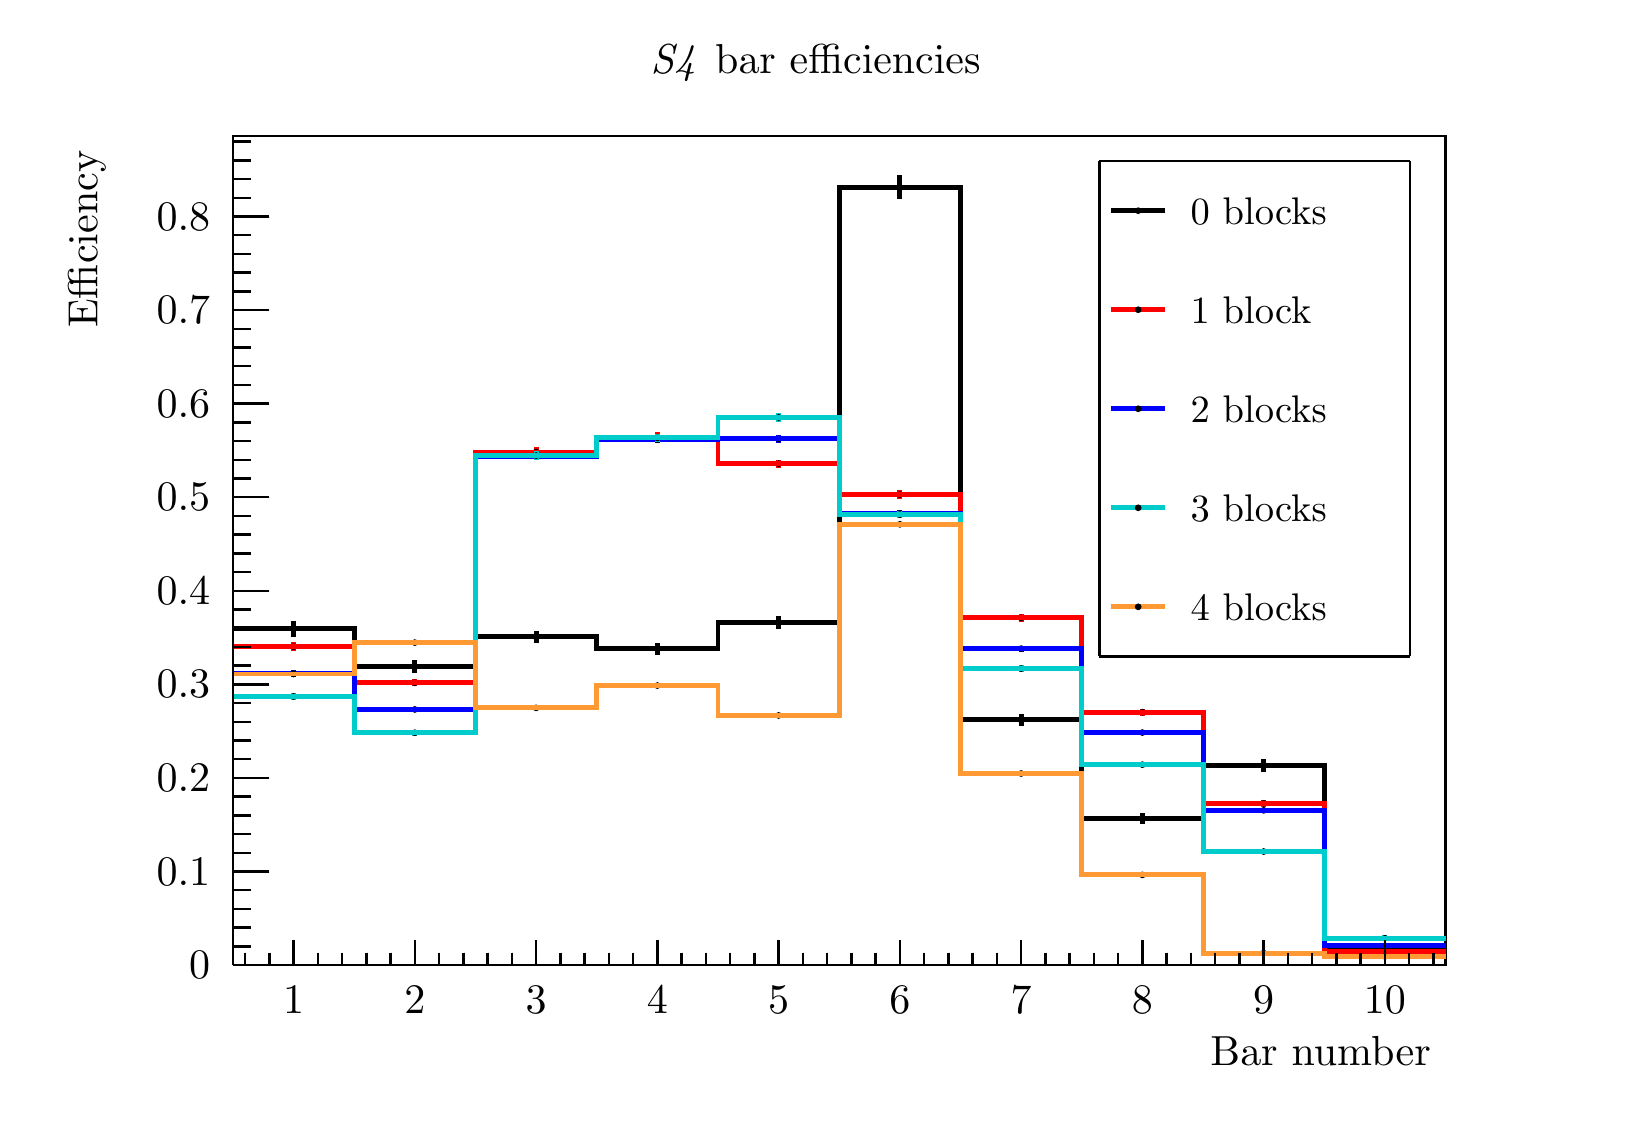
\begin{tikzpicture}
\pgfdeclareplotmark{cross} {
\pgfpathmoveto{\pgfpoint{-0.3\pgfplotmarksize}{\pgfplotmarksize}}
\pgfpathlineto{\pgfpoint{+0.3\pgfplotmarksize}{\pgfplotmarksize}}
\pgfpathlineto{\pgfpoint{+0.3\pgfplotmarksize}{0.3\pgfplotmarksize}}
\pgfpathlineto{\pgfpoint{+1\pgfplotmarksize}{0.3\pgfplotmarksize}}
\pgfpathlineto{\pgfpoint{+1\pgfplotmarksize}{-0.3\pgfplotmarksize}}
\pgfpathlineto{\pgfpoint{+0.3\pgfplotmarksize}{-0.3\pgfplotmarksize}}
\pgfpathlineto{\pgfpoint{+0.3\pgfplotmarksize}{-1.\pgfplotmarksize}}
\pgfpathlineto{\pgfpoint{-0.3\pgfplotmarksize}{-1.\pgfplotmarksize}}
\pgfpathlineto{\pgfpoint{-0.3\pgfplotmarksize}{-0.3\pgfplotmarksize}}
\pgfpathlineto{\pgfpoint{-1.\pgfplotmarksize}{-0.3\pgfplotmarksize}}
\pgfpathlineto{\pgfpoint{-1.\pgfplotmarksize}{0.3\pgfplotmarksize}}
\pgfpathlineto{\pgfpoint{-0.3\pgfplotmarksize}{0.3\pgfplotmarksize}}
\pgfpathclose
\pgfusepathqstroke
}
\pgfdeclareplotmark{cross*} {
\pgfpathmoveto{\pgfpoint{-0.3\pgfplotmarksize}{\pgfplotmarksize}}
\pgfpathlineto{\pgfpoint{+0.3\pgfplotmarksize}{\pgfplotmarksize}}
\pgfpathlineto{\pgfpoint{+0.3\pgfplotmarksize}{0.3\pgfplotmarksize}}
\pgfpathlineto{\pgfpoint{+1\pgfplotmarksize}{0.3\pgfplotmarksize}}
\pgfpathlineto{\pgfpoint{+1\pgfplotmarksize}{-0.3\pgfplotmarksize}}
\pgfpathlineto{\pgfpoint{+0.3\pgfplotmarksize}{-0.3\pgfplotmarksize}}
\pgfpathlineto{\pgfpoint{+0.3\pgfplotmarksize}{-1.\pgfplotmarksize}}
\pgfpathlineto{\pgfpoint{-0.3\pgfplotmarksize}{-1.\pgfplotmarksize}}
\pgfpathlineto{\pgfpoint{-0.3\pgfplotmarksize}{-0.3\pgfplotmarksize}}
\pgfpathlineto{\pgfpoint{-1.\pgfplotmarksize}{-0.3\pgfplotmarksize}}
\pgfpathlineto{\pgfpoint{-1.\pgfplotmarksize}{0.3\pgfplotmarksize}}
\pgfpathlineto{\pgfpoint{-0.3\pgfplotmarksize}{0.3\pgfplotmarksize}}
\pgfpathclose
\pgfusepathqfillstroke
}
\pgfdeclareplotmark{newstar} {
\pgfpathmoveto{\pgfqpoint{0pt}{\pgfplotmarksize}}
\pgfpathlineto{\pgfqpointpolar{44}{0.5\pgfplotmarksize}}
\pgfpathlineto{\pgfqpointpolar{18}{\pgfplotmarksize}}
\pgfpathlineto{\pgfqpointpolar{-20}{0.5\pgfplotmarksize}}
\pgfpathlineto{\pgfqpointpolar{-54}{\pgfplotmarksize}}
\pgfpathlineto{\pgfqpointpolar{-90}{0.5\pgfplotmarksize}}
\pgfpathlineto{\pgfqpointpolar{234}{\pgfplotmarksize}}
\pgfpathlineto{\pgfqpointpolar{198}{0.5\pgfplotmarksize}}
\pgfpathlineto{\pgfqpointpolar{162}{\pgfplotmarksize}}
\pgfpathlineto{\pgfqpointpolar{134}{0.5\pgfplotmarksize}}
\pgfpathclose
\pgfusepathqstroke
}
\pgfdeclareplotmark{newstar*} {
\pgfpathmoveto{\pgfqpoint{0pt}{\pgfplotmarksize}}
\pgfpathlineto{\pgfqpointpolar{44}{0.5\pgfplotmarksize}}
\pgfpathlineto{\pgfqpointpolar{18}{\pgfplotmarksize}}
\pgfpathlineto{\pgfqpointpolar{-20}{0.5\pgfplotmarksize}}
\pgfpathlineto{\pgfqpointpolar{-54}{\pgfplotmarksize}}
\pgfpathlineto{\pgfqpointpolar{-90}{0.5\pgfplotmarksize}}
\pgfpathlineto{\pgfqpointpolar{234}{\pgfplotmarksize}}
\pgfpathlineto{\pgfqpointpolar{198}{0.5\pgfplotmarksize}}
\pgfpathlineto{\pgfqpointpolar{162}{\pgfplotmarksize}}
\pgfpathlineto{\pgfqpointpolar{134}{0.5\pgfplotmarksize}}
\pgfpathclose
\pgfusepathqfillstroke
}
\definecolor{c}{rgb}{1,1,1};
\draw [color=c, fill=c] (0,0) rectangle (20,13.6752);
\draw [color=c, fill=c] (2.6,1.77778) rectangle (18,12.3077);
\definecolor{c}{rgb}{0,0,0};
\draw [c,line width=0.9] (2.6,1.77778) -- (2.6,12.3077) -- (18,12.3077) -- (18,1.77778) -- (2.6,1.77778);
\definecolor{c}{rgb}{1,1,1};
\draw [color=c, fill=c] (2.6,1.77778) rectangle (18,12.3077);
\definecolor{c}{rgb}{0,0,0};
\draw [c,line width=0.9] (2.6,1.77778) -- (2.6,12.3077) -- (18,12.3077) -- (18,1.77778) -- (2.6,1.77778);
\definecolor{c}{rgb}{0,0,0.6};
\draw [c,line width=0.9] (2.6,1.77778) -- (4.14,1.77778) -- (4.14,1.77778) -- (5.68,1.77778) -- (5.68,1.77778) -- (7.22,1.77778) -- (7.22,1.77778) -- (8.76,1.77778) -- (8.76,1.77778) -- (10.3,1.77778) -- (10.3,1.77778) -- (11.84,1.77778) --
 (11.84,1.77778) -- (13.38,1.77778) -- (13.38,1.77778) -- (14.92,1.77778) -- (14.92,1.77778) -- (16.46,1.77778) -- (16.46,1.77778) -- (18,1.77778);
\definecolor{c}{rgb}{0,0,0};
\draw [c,line width=0.9] (2.6,1.77778) -- (18,1.77778);
\draw [c,line width=0.9] (3.37,2.09368) -- (3.37,1.77778);
\draw [c,line width=0.9] (3.678,1.93573) -- (3.678,1.77778);
\draw [c,line width=0.9] (3.986,1.93573) -- (3.986,1.77778);
\draw [c,line width=0.9] (4.294,1.93573) -- (4.294,1.77778);
\draw [c,line width=0.9] (4.602,1.93573) -- (4.602,1.77778);
\draw [c,line width=0.9] (4.91,2.09368) -- (4.91,1.77778);
\draw [c,line width=0.9] (5.218,1.93573) -- (5.218,1.77778);
\draw [c,line width=0.9] (5.526,1.93573) -- (5.526,1.77778);
\draw [c,line width=0.9] (5.834,1.93573) -- (5.834,1.77778);
\draw [c,line width=0.9] (6.142,1.93573) -- (6.142,1.77778);
\draw [c,line width=0.9] (6.45,2.09368) -- (6.45,1.77778);
\draw [c,line width=0.9] (6.758,1.93573) -- (6.758,1.77778);
\draw [c,line width=0.9] (7.066,1.93573) -- (7.066,1.77778);
\draw [c,line width=0.9] (7.374,1.93573) -- (7.374,1.77778);
\draw [c,line width=0.9] (7.682,1.93573) -- (7.682,1.77778);
\draw [c,line width=0.9] (7.99,2.09368) -- (7.99,1.77778);
\draw [c,line width=0.9] (8.298,1.93573) -- (8.298,1.77778);
\draw [c,line width=0.9] (8.606,1.93573) -- (8.606,1.77778);
\draw [c,line width=0.9] (8.914,1.93573) -- (8.914,1.77778);
\draw [c,line width=0.9] (9.222,1.93573) -- (9.222,1.77778);
\draw [c,line width=0.9] (9.53,2.09368) -- (9.53,1.77778);
\draw [c,line width=0.9] (9.838,1.93573) -- (9.838,1.77778);
\draw [c,line width=0.9] (10.146,1.93573) -- (10.146,1.77778);
\draw [c,line width=0.9] (10.454,1.93573) -- (10.454,1.77778);
\draw [c,line width=0.9] (10.762,1.93573) -- (10.762,1.77778);
\draw [c,line width=0.9] (11.07,2.09368) -- (11.07,1.77778);
\draw [c,line width=0.9] (11.378,1.93573) -- (11.378,1.77778);
\draw [c,line width=0.9] (11.686,1.93573) -- (11.686,1.77778);
\draw [c,line width=0.9] (11.994,1.93573) -- (11.994,1.77778);
\draw [c,line width=0.9] (12.302,1.93573) -- (12.302,1.77778);
\draw [c,line width=0.9] (12.61,2.09368) -- (12.61,1.77778);
\draw [c,line width=0.9] (12.918,1.93573) -- (12.918,1.77778);
\draw [c,line width=0.9] (13.226,1.93573) -- (13.226,1.77778);
\draw [c,line width=0.9] (13.534,1.93573) -- (13.534,1.77778);
\draw [c,line width=0.9] (13.842,1.93573) -- (13.842,1.77778);
\draw [c,line width=0.9] (14.15,2.09368) -- (14.15,1.77778);
\draw [c,line width=0.9] (14.458,1.93573) -- (14.458,1.77778);
\draw [c,line width=0.9] (14.766,1.93573) -- (14.766,1.77778);
\draw [c,line width=0.9] (15.074,1.93573) -- (15.074,1.77778);
\draw [c,line width=0.9] (15.382,1.93573) -- (15.382,1.77778);
\draw [c,line width=0.9] (15.69,2.09368) -- (15.69,1.77778);
\draw [c,line width=0.9] (15.998,1.93573) -- (15.998,1.77778);
\draw [c,line width=0.9] (16.306,1.93573) -- (16.306,1.77778);
\draw [c,line width=0.9] (16.614,1.93573) -- (16.614,1.77778);
\draw [c,line width=0.9] (16.922,1.93573) -- (16.922,1.77778);
\draw [c,line width=0.9] (17.23,2.09368) -- (17.23,1.77778);
\draw [c,line width=0.9] (3.37,2.09368) -- (3.37,1.77778);
\draw [c,line width=0.9] (3.062,1.93573) -- (3.062,1.77778);
\draw [c,line width=0.9] (2.754,1.93573) -- (2.754,1.77778);
\draw [c,line width=0.9] (17.23,2.09368) -- (17.23,1.77778);
\draw [c,line width=0.9] (17.538,1.93573) -- (17.538,1.77778);
\draw [c,line width=0.9] (17.846,1.93573) -- (17.846,1.77778);
\draw [anchor=base] (3.37,1.16239) node[scale=1.51861, color=c, rotate=0]{1};
\draw [anchor=base] (4.91,1.16239) node[scale=1.51861, color=c, rotate=0]{2};
\draw [anchor=base] (6.45,1.16239) node[scale=1.51861, color=c, rotate=0]{3};
\draw [anchor=base] (7.99,1.16239) node[scale=1.51861, color=c, rotate=0]{4};
\draw [anchor=base] (9.53,1.16239) node[scale=1.51861, color=c, rotate=0]{5};
\draw [anchor=base] (11.07,1.16239) node[scale=1.51861, color=c, rotate=0]{6};
\draw [anchor=base] (12.61,1.16239) node[scale=1.51861, color=c, rotate=0]{7};
\draw [anchor=base] (14.15,1.16239) node[scale=1.51861, color=c, rotate=0]{8};
\draw [anchor=base] (15.69,1.16239) node[scale=1.51861, color=c, rotate=0]{9};
\draw [anchor=base] (17.23,1.16239) node[scale=1.51861, color=c, rotate=0]{10};
\draw [anchor= east] (18,0.683761) node[scale=1.51861, color=c, rotate=0]{ Bar number};
\draw [c,line width=0.9] (2.6,1.77778) -- (2.6,12.3077);
\draw [c,line width=0.9] (3.062,1.77778) -- (2.6,1.77778);
\draw [c,line width=0.9] (2.831,2.01544) -- (2.6,2.01544);
\draw [c,line width=0.9] (2.831,2.2531) -- (2.6,2.2531);
\draw [c,line width=0.9] (2.831,2.49075) -- (2.6,2.49075);
\draw [c,line width=0.9] (2.831,2.72841) -- (2.6,2.72841);
\draw [c,line width=0.9] (3.062,2.96607) -- (2.6,2.96607);
\draw [c,line width=0.9] (2.831,3.20373) -- (2.6,3.20373);
\draw [c,line width=0.9] (2.831,3.44139) -- (2.6,3.44139);
\draw [c,line width=0.9] (2.831,3.67905) -- (2.6,3.67905);
\draw [c,line width=0.9] (2.831,3.91671) -- (2.6,3.91671);
\draw [c,line width=0.9] (3.062,4.15437) -- (2.6,4.15437);
\draw [c,line width=0.9] (2.831,4.39202) -- (2.6,4.39202);
\draw [c,line width=0.9] (2.831,4.62968) -- (2.6,4.62968);
\draw [c,line width=0.9] (2.831,4.86734) -- (2.6,4.86734);
\draw [c,line width=0.9] (2.831,5.105) -- (2.6,5.105);
\draw [c,line width=0.9] (3.062,5.34266) -- (2.6,5.34266);
\draw [c,line width=0.9] (2.831,5.58032) -- (2.6,5.58032);
\draw [c,line width=0.9] (2.831,5.81798) -- (2.6,5.81798);
\draw [c,line width=0.9] (2.831,6.05563) -- (2.6,6.05563);
\draw [c,line width=0.9] (2.831,6.29329) -- (2.6,6.29329);
\draw [c,line width=0.9] (3.062,6.53095) -- (2.6,6.53095);
\draw [c,line width=0.9] (2.831,6.76861) -- (2.6,6.76861);
\draw [c,line width=0.9] (2.831,7.00627) -- (2.6,7.00627);
\draw [c,line width=0.9] (2.831,7.24393) -- (2.6,7.24393);
\draw [c,line width=0.9] (2.831,7.48159) -- (2.6,7.48159);
\draw [c,line width=0.9] (3.062,7.71925) -- (2.6,7.71925);
\draw [c,line width=0.9] (2.831,7.9569) -- (2.6,7.9569);
\draw [c,line width=0.9] (2.831,8.19456) -- (2.6,8.19456);
\draw [c,line width=0.9] (2.831,8.43222) -- (2.6,8.43222);
\draw [c,line width=0.9] (2.831,8.66988) -- (2.6,8.66988);
\draw [c,line width=0.9] (3.062,8.90754) -- (2.6,8.90754);
\draw [c,line width=0.9] (2.831,9.1452) -- (2.6,9.1452);
\draw [c,line width=0.9] (2.831,9.38286) -- (2.6,9.38286);
\draw [c,line width=0.9] (2.831,9.62052) -- (2.6,9.62052);
\draw [c,line width=0.9] (2.831,9.85817) -- (2.6,9.85817);
\draw [c,line width=0.9] (3.062,10.0958) -- (2.6,10.0958);
\draw [c,line width=0.9] (2.831,10.3335) -- (2.6,10.3335);
\draw [c,line width=0.9] (2.831,10.5711) -- (2.6,10.5711);
\draw [c,line width=0.9] (2.831,10.8088) -- (2.6,10.8088);
\draw [c,line width=0.9] (2.831,11.0465) -- (2.6,11.0465);
\draw [c,line width=0.9] (3.062,11.2841) -- (2.6,11.2841);
\draw [c,line width=0.9] (3.062,11.2841) -- (2.6,11.2841);
\draw [c,line width=0.9] (2.831,11.5218) -- (2.6,11.5218);
\draw [c,line width=0.9] (2.831,11.7594) -- (2.6,11.7594);
\draw [c,line width=0.9] (2.831,11.9971) -- (2.6,11.9971);
\draw [c,line width=0.9] (2.831,12.2348) -- (2.6,12.2348);
\draw [anchor= east] (2.5,1.77778) node[scale=1.51861, color=c, rotate=0]{0};
\draw [anchor= east] (2.5,2.96607) node[scale=1.51861, color=c, rotate=0]{0.1};
\draw [anchor= east] (2.5,4.15437) node[scale=1.51861, color=c, rotate=0]{0.2};
\draw [anchor= east] (2.5,5.34266) node[scale=1.51861, color=c, rotate=0]{0.3};
\draw [anchor= east] (2.5,6.53095) node[scale=1.51861, color=c, rotate=0]{0.4};
\draw [anchor= east] (2.5,7.71925) node[scale=1.51861, color=c, rotate=0]{0.5};
\draw [anchor= east] (2.5,8.90754) node[scale=1.51861, color=c, rotate=0]{0.6};
\draw [anchor= east] (2.5,10.0958) node[scale=1.51861, color=c, rotate=0]{0.7};
\draw [anchor= east] (2.5,11.2841) node[scale=1.51861, color=c, rotate=0]{0.8};
\draw [anchor= east] (0.745299,12.3077) node[scale=1.51861, color=c, rotate=90]{ Efficiency};
\draw [c,line width=1.8] (3.37,5.94713) -- (3.37,6.048);
\draw [c,line width=1.8] (3.37,6.048) -- (3.37,6.14887);
\foreach \P in {(3.37,6.048)}{\draw[mark options={color=c,fill=c},mark size=2.402402pt,mark=*,mark size=1pt] plot coordinates {\P};}
\draw [c,line width=1.8] (4.91,5.48652) -- (4.91,5.56707);
\draw [c,line width=1.8] (4.91,5.56707) -- (4.91,5.64763);
\foreach \P in {(4.91,5.56707)}{\draw[mark options={color=c,fill=c},mark size=2.402402pt,mark=*,mark size=1pt] plot coordinates {\P};}
\draw [c,line width=1.8] (6.45,5.86443) -- (6.45,5.94509);
\draw [c,line width=1.8] (6.45,5.94509) -- (6.45,6.02574);
\foreach \P in {(6.45,5.94509)}{\draw[mark options={color=c,fill=c},mark size=2.402402pt,mark=*,mark size=1pt] plot coordinates {\P};}
\draw [c,line width=1.8] (7.99,5.72099) -- (7.99,5.79421);
\draw [c,line width=1.8] (7.99,5.79421) -- (7.99,5.86742);
\foreach \P in {(7.99,5.79421)}{\draw[mark options={color=c,fill=c},mark size=2.402402pt,mark=*,mark size=1pt] plot coordinates {\P};}
\draw [c,line width=1.8] (9.53,6.04947) -- (9.53,6.12746);
\draw [c,line width=1.8] (9.53,6.12746) -- (9.53,6.20546);
\foreach \P in {(9.53,6.12746)}{\draw[mark options={color=c,fill=c},mark size=2.402402pt,mark=*,mark size=1pt] plot coordinates {\P};}
\draw [c,line width=1.8] (11.07,11.5047) -- (11.07,11.6555);
\draw [c,line width=1.8] (11.07,11.6555) -- (11.07,11.8063);
\foreach \P in {(11.07,11.6555)}{\draw[mark options={color=c,fill=c},mark size=2.402402pt,mark=*,mark size=1pt] plot coordinates {\P};}
\draw [c,line width=1.8] (12.61,4.81396) -- (12.61,4.88993);
\draw [c,line width=1.8] (12.61,4.88993) -- (12.61,4.96589);
\foreach \P in {(12.61,4.88993)}{\draw[mark options={color=c,fill=c},mark size=2.402402pt,mark=*,mark size=1pt] plot coordinates {\P};}
\draw [c,line width=1.8] (14.15,3.56561) -- (14.15,3.63618);
\draw [c,line width=1.8] (14.15,3.63618) -- (14.15,3.70674);
\foreach \P in {(14.15,3.63618)}{\draw[mark options={color=c,fill=c},mark size=2.402402pt,mark=*,mark size=1pt] plot coordinates {\P};}
\draw [c,line width=1.8] (15.69,4.23443) -- (15.69,4.31531);
\draw [c,line width=1.8] (15.69,4.31531) -- (15.69,4.39619);
\foreach \P in {(15.69,4.31531)}{\draw[mark options={color=c,fill=c},mark size=2.402402pt,mark=*,mark size=1pt] plot coordinates {\P};}
\draw [c,line width=1.8] (17.23,1.95841) -- (17.23,2.00004);
\draw [c,line width=1.8] (17.23,2.00004) -- (17.23,2.04166);
\foreach \P in {(17.23,2.00004)}{\draw[mark options={color=c,fill=c},mark size=2.402402pt,mark=*,mark size=1pt] plot coordinates {\P};}
\draw [c,line width=1.8] (2.6,6.048) -- (4.14,6.048) -- (4.14,5.56707) -- (5.68,5.56707) -- (5.68,5.94509) -- (7.22,5.94509) -- (7.22,5.79421) -- (8.76,5.79421) -- (8.76,6.12746) -- (10.3,6.12746) -- (10.3,11.6555) -- (11.84,11.6555) --
 (11.84,4.88993) -- (13.38,4.88993) -- (13.38,3.63618) -- (14.92,3.63618) -- (14.92,4.31531) -- (16.46,4.31531) -- (16.46,2.00004) -- (18,2.00004);
\definecolor{c}{rgb}{1,0,0};
\draw [c,line width=1.8] (3.37,5.76471) -- (3.37,5.8214);
\draw [c,line width=1.8] (3.37,5.8214) -- (3.37,5.8781);
\definecolor{c}{rgb}{0,0,0};
\foreach \P in {(3.37,5.8214)}{\draw[mark options={color=c,fill=c},mark size=2.402402pt,mark=*,mark size=1pt] plot coordinates {\P};}
\definecolor{c}{rgb}{1,0,0};
\draw [c,line width=1.8] (4.91,5.31634) -- (4.91,5.36213);
\draw [c,line width=1.8] (4.91,5.36213) -- (4.91,5.40793);
\definecolor{c}{rgb}{0,0,0};
\foreach \P in {(4.91,5.36213)}{\draw[mark options={color=c,fill=c},mark size=2.402402pt,mark=*,mark size=1pt] plot coordinates {\P};}
\definecolor{c}{rgb}{1,0,0};
\draw [c,line width=1.8] (6.45,8.23172) -- (6.45,8.29272);
\draw [c,line width=1.8] (6.45,8.29272) -- (6.45,8.35373);
\definecolor{c}{rgb}{0,0,0};
\foreach \P in {(6.45,8.29272)}{\draw[mark options={color=c,fill=c},mark size=2.402402pt,mark=*,mark size=1pt] plot coordinates {\P};}
\definecolor{c}{rgb}{1,0,0};
\draw [c,line width=1.8] (7.99,8.42349) -- (7.99,8.48284);
\draw [c,line width=1.8] (7.99,8.48284) -- (7.99,8.5422);
\definecolor{c}{rgb}{0,0,0};
\foreach \P in {(7.99,8.48284)}{\draw[mark options={color=c,fill=c},mark size=2.402402pt,mark=*,mark size=1pt] plot coordinates {\P};}
\definecolor{c}{rgb}{1,0,0};
\draw [c,line width=1.8] (9.53,8.09169) -- (9.53,8.14475);
\draw [c,line width=1.8] (9.53,8.14475) -- (9.53,8.1978);
\definecolor{c}{rgb}{0,0,0};
\foreach \P in {(9.53,8.14475)}{\draw[mark options={color=c,fill=c},mark size=2.402402pt,mark=*,mark size=1pt] plot coordinates {\P};}
\definecolor{c}{rgb}{1,0,0};
\draw [c,line width=1.8] (11.07,7.69589) -- (11.07,7.75308);
\draw [c,line width=1.8] (11.07,7.75308) -- (11.07,7.81026);
\definecolor{c}{rgb}{0,0,0};
\foreach \P in {(11.07,7.75308)}{\draw[mark options={color=c,fill=c},mark size=2.402402pt,mark=*,mark size=1pt] plot coordinates {\P};}
\definecolor{c}{rgb}{1,0,0};
\draw [c,line width=1.8] (12.61,6.13603) -- (12.61,6.1871);
\draw [c,line width=1.8] (12.61,6.1871) -- (12.61,6.23818);
\definecolor{c}{rgb}{0,0,0};
\foreach \P in {(12.61,6.1871)}{\draw[mark options={color=c,fill=c},mark size=2.402402pt,mark=*,mark size=1pt] plot coordinates {\P};}
\definecolor{c}{rgb}{1,0,0};
\draw [c,line width=1.8] (14.15,4.9422) -- (14.15,4.9889);
\draw [c,line width=1.8] (14.15,4.9889) -- (14.15,5.0356);
\definecolor{c}{rgb}{0,0,0};
\foreach \P in {(14.15,4.9889)}{\draw[mark options={color=c,fill=c},mark size=2.402402pt,mark=*,mark size=1pt] plot coordinates {\P};}
\definecolor{c}{rgb}{1,0,0};
\draw [c,line width=1.8] (15.69,3.78842) -- (15.69,3.83138);
\draw [c,line width=1.8] (15.69,3.83138) -- (15.69,3.87434);
\definecolor{c}{rgb}{0,0,0};
\foreach \P in {(15.69,3.83138)}{\draw[mark options={color=c,fill=c},mark size=2.402402pt,mark=*,mark size=1pt] plot coordinates {\P};}
\definecolor{c}{rgb}{1,0,0};
\draw [c,line width=1.8] (17.23,1.91836) -- (17.23,1.9483);
\draw [c,line width=1.8] (17.23,1.9483) -- (17.23,1.97823);
\definecolor{c}{rgb}{0,0,0};
\foreach \P in {(17.23,1.9483)}{\draw[mark options={color=c,fill=c},mark size=2.402402pt,mark=*,mark size=1pt] plot coordinates {\P};}
\definecolor{c}{rgb}{1,0,0};
\draw [c,line width=1.8] (2.6,5.8214) -- (4.14,5.8214) -- (4.14,5.36213) -- (5.68,5.36213) -- (5.68,8.29272) -- (7.22,8.29272) -- (7.22,8.48284) -- (8.76,8.48284) -- (8.76,8.14475) -- (10.3,8.14475) -- (10.3,7.75308) -- (11.84,7.75308) --
 (11.84,6.1871) -- (13.38,6.1871) -- (13.38,4.9889) -- (14.92,4.9889) -- (14.92,3.83138) -- (16.46,3.83138) -- (16.46,1.9483) -- (18,1.9483);
\definecolor{c}{rgb}{0,0,1};
\draw [c,line width=1.8] (3.37,5.43835) -- (3.37,5.48052);
\draw [c,line width=1.8] (3.37,5.48052) -- (3.37,5.52268);
\definecolor{c}{rgb}{0,0,0};
\foreach \P in {(3.37,5.48052)}{\draw[mark options={color=c,fill=c},mark size=2.402402pt,mark=*,mark size=1pt] plot coordinates {\P};}
\definecolor{c}{rgb}{0,0,1};
\draw [c,line width=1.8] (4.91,4.9892) -- (4.91,5.02356);
\draw [c,line width=1.8] (4.91,5.02356) -- (4.91,5.05792);
\definecolor{c}{rgb}{0,0,0};
\foreach \P in {(4.91,5.02356)}{\draw[mark options={color=c,fill=c},mark size=2.402402pt,mark=*,mark size=1pt] plot coordinates {\P};}
\definecolor{c}{rgb}{0,0,1};
\draw [c,line width=1.8] (6.45,8.19027) -- (6.45,8.23881);
\draw [c,line width=1.8] (6.45,8.23881) -- (6.45,8.28735);
\definecolor{c}{rgb}{0,0,0};
\foreach \P in {(6.45,8.23881)}{\draw[mark options={color=c,fill=c},mark size=2.402402pt,mark=*,mark size=1pt] plot coordinates {\P};}
\definecolor{c}{rgb}{0,0,1};
\draw [c,line width=1.8] (7.99,8.40121) -- (7.99,8.44901);
\draw [c,line width=1.8] (7.99,8.44901) -- (7.99,8.49681);
\definecolor{c}{rgb}{0,0,0};
\foreach \P in {(7.99,8.44901)}{\draw[mark options={color=c,fill=c},mark size=2.402402pt,mark=*,mark size=1pt] plot coordinates {\P};}
\definecolor{c}{rgb}{0,0,1};
\draw [c,line width=1.8] (9.53,8.41363) -- (9.53,8.45921);
\draw [c,line width=1.8] (9.53,8.45921) -- (9.53,8.50478);
\definecolor{c}{rgb}{0,0,0};
\foreach \P in {(9.53,8.45921)}{\draw[mark options={color=c,fill=c},mark size=2.402402pt,mark=*,mark size=1pt] plot coordinates {\P};}
\definecolor{c}{rgb}{0,0,1};
\draw [c,line width=1.8] (11.07,7.46957) -- (11.07,7.51425);
\draw [c,line width=1.8] (11.07,7.51425) -- (11.07,7.55892);
\definecolor{c}{rgb}{0,0,0};
\foreach \P in {(11.07,7.51425)}{\draw[mark options={color=c,fill=c},mark size=2.402402pt,mark=*,mark size=1pt] plot coordinates {\P};}
\definecolor{c}{rgb}{0,0,1};
\draw [c,line width=1.8] (12.61,5.75818) -- (12.61,5.79638);
\draw [c,line width=1.8] (12.61,5.79638) -- (12.61,5.83458);
\definecolor{c}{rgb}{0,0,0};
\foreach \P in {(12.61,5.79638)}{\draw[mark options={color=c,fill=c},mark size=2.402402pt,mark=*,mark size=1pt] plot coordinates {\P};}
\definecolor{c}{rgb}{0,0,1};
\draw [c,line width=1.8] (14.15,4.69542) -- (14.15,4.73);
\draw [c,line width=1.8] (14.15,4.73) -- (14.15,4.76458);
\definecolor{c}{rgb}{0,0,0};
\foreach \P in {(14.15,4.73)}{\draw[mark options={color=c,fill=c},mark size=2.402402pt,mark=*,mark size=1pt] plot coordinates {\P};}
\definecolor{c}{rgb}{0,0,1};
\draw [c,line width=1.8] (15.69,3.71002) -- (15.69,3.74208);
\draw [c,line width=1.8] (15.69,3.74208) -- (15.69,3.77415);
\definecolor{c}{rgb}{0,0,0};
\foreach \P in {(15.69,3.74208)}{\draw[mark options={color=c,fill=c},mark size=2.402402pt,mark=*,mark size=1pt] plot coordinates {\P};}
\definecolor{c}{rgb}{0,0,1};
\draw [c,line width=1.8] (17.23,1.99459) -- (17.23,2.02279);
\draw [c,line width=1.8] (17.23,2.02279) -- (17.23,2.05099);
\definecolor{c}{rgb}{0,0,0};
\foreach \P in {(17.23,2.02279)}{\draw[mark options={color=c,fill=c},mark size=2.402402pt,mark=*,mark size=1pt] plot coordinates {\P};}
\definecolor{c}{rgb}{0,0,1};
\draw [c,line width=1.8] (2.6,5.48052) -- (4.14,5.48052) -- (4.14,5.02356) -- (5.68,5.02356) -- (5.68,8.23881) -- (7.22,8.23881) -- (7.22,8.44901) -- (8.76,8.44901) -- (8.76,8.45921) -- (10.3,8.45921) -- (10.3,7.51425) -- (11.84,7.51425) --
 (11.84,5.79638) -- (13.38,5.79638) -- (13.38,4.73) -- (14.92,4.73) -- (14.92,3.74208) -- (16.46,3.74208) -- (16.46,2.02279) -- (18,2.02279);
\definecolor{c}{rgb}{0,0.8,0.8};
\draw [c,line width=1.8] (3.37,5.14512) -- (3.37,5.18859);
\draw [c,line width=1.8] (3.37,5.18859) -- (3.37,5.23205);
\definecolor{c}{rgb}{0,0,0};
\foreach \P in {(3.37,5.18859)}{\draw[mark options={color=c,fill=c},mark size=2.402402pt,mark=*,mark size=1pt] plot coordinates {\P};}
\definecolor{c}{rgb}{0,0.8,0.8};
\draw [c,line width=1.8] (4.91,4.69231) -- (4.91,4.72802);
\draw [c,line width=1.8] (4.91,4.72802) -- (4.91,4.76372);
\definecolor{c}{rgb}{0,0,0};
\foreach \P in {(4.91,4.72802)}{\draw[mark options={color=c,fill=c},mark size=2.402402pt,mark=*,mark size=1pt] plot coordinates {\P};}
\definecolor{c}{rgb}{0,0.8,0.8};
\draw [c,line width=1.8] (6.45,8.19462) -- (6.45,8.2476);
\draw [c,line width=1.8] (6.45,8.2476) -- (6.45,8.30059);
\definecolor{c}{rgb}{0,0,0};
\foreach \P in {(6.45,8.2476)}{\draw[mark options={color=c,fill=c},mark size=2.402402pt,mark=*,mark size=1pt] plot coordinates {\P};}
\definecolor{c}{rgb}{0,0.8,0.8};
\draw [c,line width=1.8] (7.99,8.41839) -- (7.99,8.47122);
\draw [c,line width=1.8] (7.99,8.47122) -- (7.99,8.52405);
\definecolor{c}{rgb}{0,0,0};
\foreach \P in {(7.99,8.47122)}{\draw[mark options={color=c,fill=c},mark size=2.402402pt,mark=*,mark size=1pt] plot coordinates {\P};}
\definecolor{c}{rgb}{0,0.8,0.8};
\draw [c,line width=1.8] (9.53,8.67919) -- (9.53,8.73184);
\draw [c,line width=1.8] (9.53,8.73184) -- (9.53,8.78449);
\definecolor{c}{rgb}{0,0,0};
\foreach \P in {(9.53,8.73184)}{\draw[mark options={color=c,fill=c},mark size=2.402402pt,mark=*,mark size=1pt] plot coordinates {\P};}
\definecolor{c}{rgb}{0,0.8,0.8};
\draw [c,line width=1.8] (11.07,7.44878) -- (11.07,7.49768);
\draw [c,line width=1.8] (11.07,7.49768) -- (11.07,7.54658);
\definecolor{c}{rgb}{0,0,0};
\foreach \P in {(11.07,7.49768)}{\draw[mark options={color=c,fill=c},mark size=2.402402pt,mark=*,mark size=1pt] plot coordinates {\P};}
\definecolor{c}{rgb}{0,0.8,0.8};
\draw [c,line width=1.8] (12.61,5.50194) -- (12.61,5.54215);
\draw [c,line width=1.8] (12.61,5.54215) -- (12.61,5.58236);
\definecolor{c}{rgb}{0,0,0};
\foreach \P in {(12.61,5.54215)}{\draw[mark options={color=c,fill=c},mark size=2.402402pt,mark=*,mark size=1pt] plot coordinates {\P};}
\definecolor{c}{rgb}{0,0.8,0.8};
\draw [c,line width=1.8] (14.15,4.28775) -- (14.15,4.32232);
\draw [c,line width=1.8] (14.15,4.32232) -- (14.15,4.3569);
\definecolor{c}{rgb}{0,0,0};
\foreach \P in {(14.15,4.32232)}{\draw[mark options={color=c,fill=c},mark size=2.402402pt,mark=*,mark size=1pt] plot coordinates {\P};}
\definecolor{c}{rgb}{0,0.8,0.8};
\draw [c,line width=1.8] (15.69,3.18971) -- (15.69,3.21924);
\draw [c,line width=1.8] (15.69,3.21924) -- (15.69,3.24878);
\definecolor{c}{rgb}{0,0,0};
\foreach \P in {(15.69,3.21924)}{\draw[mark options={color=c,fill=c},mark size=2.402402pt,mark=*,mark size=1pt] plot coordinates {\P};}
\definecolor{c}{rgb}{0,0.8,0.8};
\draw [c,line width=1.8] (17.23,2.07797) -- (17.23,2.11716);
\draw [c,line width=1.8] (17.23,2.11716) -- (17.23,2.15634);
\definecolor{c}{rgb}{0,0,0};
\foreach \P in {(17.23,2.11716)}{\draw[mark options={color=c,fill=c},mark size=2.402402pt,mark=*,mark size=1pt] plot coordinates {\P};}
\definecolor{c}{rgb}{0,0.8,0.8};
\draw [c,line width=1.8] (2.6,5.18859) -- (4.14,5.18859) -- (4.14,4.72802) -- (5.68,4.72802) -- (5.68,8.2476) -- (7.22,8.2476) -- (7.22,8.47122) -- (8.76,8.47122) -- (8.76,8.73184) -- (10.3,8.73184) -- (10.3,7.49768) -- (11.84,7.49768) --
 (11.84,5.54215) -- (13.38,5.54215) -- (13.38,4.32232) -- (14.92,4.32232) -- (14.92,3.21924) -- (16.46,3.21924) -- (16.46,2.11716) -- (18,2.11716);
\definecolor{c}{rgb}{1,0.6,0.2};
\draw [c,line width=1.8] (3.37,5.46131) -- (3.37,5.47379);
\draw [c,line width=1.8] (3.37,5.47379) -- (3.37,5.48626);
\definecolor{c}{rgb}{0,0,0};
\foreach \P in {(3.37,5.47379)}{\draw[mark options={color=c,fill=c},mark size=2.402402pt,mark=*,mark size=1pt] plot coordinates {\P};}
\definecolor{c}{rgb}{1,0.6,0.2};
\draw [c,line width=1.8] (4.91,5.86106) -- (4.91,5.8726);
\draw [c,line width=1.8] (4.91,5.8726) -- (4.91,5.88414);
\definecolor{c}{rgb}{0,0,0};
\foreach \P in {(4.91,5.8726)}{\draw[mark options={color=c,fill=c},mark size=2.402402pt,mark=*,mark size=1pt] plot coordinates {\P};}
\definecolor{c}{rgb}{1,0.6,0.2};
\draw [c,line width=1.8] (6.45,5.03364) -- (6.45,5.04378);
\draw [c,line width=1.8] (6.45,5.04378) -- (6.45,5.05392);
\definecolor{c}{rgb}{0,0,0};
\foreach \P in {(6.45,5.04378)}{\draw[mark options={color=c,fill=c},mark size=2.402402pt,mark=*,mark size=1pt] plot coordinates {\P};}
\definecolor{c}{rgb}{1,0.6,0.2};
\draw [c,line width=1.8] (7.99,5.31713) -- (7.99,5.32715);
\draw [c,line width=1.8] (7.99,5.32715) -- (7.99,5.33717);
\definecolor{c}{rgb}{0,0,0};
\foreach \P in {(7.99,5.32715)}{\draw[mark options={color=c,fill=c},mark size=2.402402pt,mark=*,mark size=1pt] plot coordinates {\P};}
\definecolor{c}{rgb}{1,0.6,0.2};
\draw [c,line width=1.8] (9.53,4.93765) -- (9.53,4.94748);
\draw [c,line width=1.8] (9.53,4.94748) -- (9.53,4.9573);
\definecolor{c}{rgb}{0,0,0};
\foreach \P in {(9.53,4.94748)}{\draw[mark options={color=c,fill=c},mark size=2.402402pt,mark=*,mark size=1pt] plot coordinates {\P};}
\definecolor{c}{rgb}{1,0.6,0.2};
\draw [c,line width=1.8] (11.07,7.36086) -- (11.07,7.37486);
\draw [c,line width=1.8] (11.07,7.37486) -- (11.07,7.38885);
\definecolor{c}{rgb}{0,0,0};
\foreach \P in {(11.07,7.37486)}{\draw[mark options={color=c,fill=c},mark size=2.402402pt,mark=*,mark size=1pt] plot coordinates {\P};}
\definecolor{c}{rgb}{1,0.6,0.2};
\draw [c,line width=1.8] (12.61,4.20077) -- (12.61,4.21019);
\draw [c,line width=1.8] (12.61,4.21019) -- (12.61,4.21961);
\definecolor{c}{rgb}{0,0,0};
\foreach \P in {(12.61,4.21019)}{\draw[mark options={color=c,fill=c},mark size=2.402402pt,mark=*,mark size=1pt] plot coordinates {\P};}
\definecolor{c}{rgb}{1,0.6,0.2};
\draw [c,line width=1.8] (14.15,2.91481) -- (14.15,2.92264);
\draw [c,line width=1.8] (14.15,2.92264) -- (14.15,2.93048);
\definecolor{c}{rgb}{0,0,0};
\foreach \P in {(14.15,2.92264)}{\draw[mark options={color=c,fill=c},mark size=2.402402pt,mark=*,mark size=1pt] plot coordinates {\P};}
\definecolor{c}{rgb}{1,0.6,0.2};
\draw [c,line width=1.8] (15.69,1.92646) -- (15.69,1.92916);
\draw [c,line width=1.8] (15.69,1.92916) -- (15.69,1.93185);
\definecolor{c}{rgb}{0,0,0};
\foreach \P in {(15.69,1.92916)}{\draw[mark options={color=c,fill=c},mark size=2.402402pt,mark=*,mark size=1pt] plot coordinates {\P};}
\definecolor{c}{rgb}{1,0.6,0.2};
\draw [c,line width=1.8] (17.23,1.88299) -- (17.23,1.88783);
\draw [c,line width=1.8] (17.23,1.88783) -- (17.23,1.89268);
\definecolor{c}{rgb}{0,0,0};
\foreach \P in {(17.23,1.88783)}{\draw[mark options={color=c,fill=c},mark size=2.402402pt,mark=*,mark size=1pt] plot coordinates {\P};}
\definecolor{c}{rgb}{1,0.6,0.2};
\draw [c,line width=1.8] (2.6,5.47379) -- (4.14,5.47379) -- (4.14,5.8726) -- (5.68,5.8726) -- (5.68,5.04378) -- (7.22,5.04378) -- (7.22,5.32715) -- (8.76,5.32715) -- (8.76,4.94748) -- (10.3,4.94748) -- (10.3,7.37486) -- (11.84,7.37486) --
 (11.84,4.21019) -- (13.38,4.21019) -- (13.38,2.92264) -- (14.92,2.92264) -- (14.92,1.92916) -- (16.46,1.92916) -- (16.46,1.88783) -- (18,1.88783);
\definecolor{c}{rgb}{0,0,0};
\draw [c,line width=0.9] (2.6,1.77778) -- (18,1.77778);
\draw [c,line width=0.9] (3.37,2.09368) -- (3.37,1.77778);
\draw [c,line width=0.9] (3.678,1.93573) -- (3.678,1.77778);
\draw [c,line width=0.9] (3.986,1.93573) -- (3.986,1.77778);
\draw [c,line width=0.9] (4.294,1.93573) -- (4.294,1.77778);
\draw [c,line width=0.9] (4.602,1.93573) -- (4.602,1.77778);
\draw [c,line width=0.9] (4.91,2.09368) -- (4.91,1.77778);
\draw [c,line width=0.9] (5.218,1.93573) -- (5.218,1.77778);
\draw [c,line width=0.9] (5.526,1.93573) -- (5.526,1.77778);
\draw [c,line width=0.9] (5.834,1.93573) -- (5.834,1.77778);
\draw [c,line width=0.9] (6.142,1.93573) -- (6.142,1.77778);
\draw [c,line width=0.9] (6.45,2.09368) -- (6.45,1.77778);
\draw [c,line width=0.9] (6.758,1.93573) -- (6.758,1.77778);
\draw [c,line width=0.9] (7.066,1.93573) -- (7.066,1.77778);
\draw [c,line width=0.9] (7.374,1.93573) -- (7.374,1.77778);
\draw [c,line width=0.9] (7.682,1.93573) -- (7.682,1.77778);
\draw [c,line width=0.9] (7.99,2.09368) -- (7.99,1.77778);
\draw [c,line width=0.9] (8.298,1.93573) -- (8.298,1.77778);
\draw [c,line width=0.9] (8.606,1.93573) -- (8.606,1.77778);
\draw [c,line width=0.9] (8.914,1.93573) -- (8.914,1.77778);
\draw [c,line width=0.9] (9.222,1.93573) -- (9.222,1.77778);
\draw [c,line width=0.9] (9.53,2.09368) -- (9.53,1.77778);
\draw [c,line width=0.9] (9.838,1.93573) -- (9.838,1.77778);
\draw [c,line width=0.9] (10.146,1.93573) -- (10.146,1.77778);
\draw [c,line width=0.9] (10.454,1.93573) -- (10.454,1.77778);
\draw [c,line width=0.9] (10.762,1.93573) -- (10.762,1.77778);
\draw [c,line width=0.9] (11.07,2.09368) -- (11.07,1.77778);
\draw [c,line width=0.9] (11.378,1.93573) -- (11.378,1.77778);
\draw [c,line width=0.9] (11.686,1.93573) -- (11.686,1.77778);
\draw [c,line width=0.9] (11.994,1.93573) -- (11.994,1.77778);
\draw [c,line width=0.9] (12.302,1.93573) -- (12.302,1.77778);
\draw [c,line width=0.9] (12.61,2.09368) -- (12.61,1.77778);
\draw [c,line width=0.9] (12.918,1.93573) -- (12.918,1.77778);
\draw [c,line width=0.9] (13.226,1.93573) -- (13.226,1.77778);
\draw [c,line width=0.9] (13.534,1.93573) -- (13.534,1.77778);
\draw [c,line width=0.9] (13.842,1.93573) -- (13.842,1.77778);
\draw [c,line width=0.9] (14.15,2.09368) -- (14.15,1.77778);
\draw [c,line width=0.9] (14.458,1.93573) -- (14.458,1.77778);
\draw [c,line width=0.9] (14.766,1.93573) -- (14.766,1.77778);
\draw [c,line width=0.9] (15.074,1.93573) -- (15.074,1.77778);
\draw [c,line width=0.9] (15.382,1.93573) -- (15.382,1.77778);
\draw [c,line width=0.9] (15.69,2.09368) -- (15.69,1.77778);
\draw [c,line width=0.9] (15.998,1.93573) -- (15.998,1.77778);
\draw [c,line width=0.9] (16.306,1.93573) -- (16.306,1.77778);
\draw [c,line width=0.9] (16.614,1.93573) -- (16.614,1.77778);
\draw [c,line width=0.9] (16.922,1.93573) -- (16.922,1.77778);
\draw [c,line width=0.9] (17.23,2.09368) -- (17.23,1.77778);
\draw [c,line width=0.9] (3.37,2.09368) -- (3.37,1.77778);
\draw [c,line width=0.9] (3.062,1.93573) -- (3.062,1.77778);
\draw [c,line width=0.9] (2.754,1.93573) -- (2.754,1.77778);
\draw [c,line width=0.9] (17.23,2.09368) -- (17.23,1.77778);
\draw [c,line width=0.9] (17.538,1.93573) -- (17.538,1.77778);
\draw [c,line width=0.9] (17.846,1.93573) -- (17.846,1.77778);
\draw [c,line width=0.9] (2.6,1.77778) -- (2.6,12.3077);
\draw [c,line width=0.9] (3.062,1.77778) -- (2.6,1.77778);
\draw [c,line width=0.9] (2.831,2.01544) -- (2.6,2.01544);
\draw [c,line width=0.9] (2.831,2.2531) -- (2.6,2.2531);
\draw [c,line width=0.9] (2.831,2.49075) -- (2.6,2.49075);
\draw [c,line width=0.9] (2.831,2.72841) -- (2.6,2.72841);
\draw [c,line width=0.9] (3.062,2.96607) -- (2.6,2.96607);
\draw [c,line width=0.9] (2.831,3.20373) -- (2.6,3.20373);
\draw [c,line width=0.9] (2.831,3.44139) -- (2.6,3.44139);
\draw [c,line width=0.9] (2.831,3.67905) -- (2.6,3.67905);
\draw [c,line width=0.9] (2.831,3.91671) -- (2.6,3.91671);
\draw [c,line width=0.9] (3.062,4.15437) -- (2.6,4.15437);
\draw [c,line width=0.9] (2.831,4.39202) -- (2.6,4.39202);
\draw [c,line width=0.9] (2.831,4.62968) -- (2.6,4.62968);
\draw [c,line width=0.9] (2.831,4.86734) -- (2.6,4.86734);
\draw [c,line width=0.9] (2.831,5.105) -- (2.6,5.105);
\draw [c,line width=0.9] (3.062,5.34266) -- (2.6,5.34266);
\draw [c,line width=0.9] (2.831,5.58032) -- (2.6,5.58032);
\draw [c,line width=0.9] (2.831,5.81798) -- (2.6,5.81798);
\draw [c,line width=0.9] (2.831,6.05563) -- (2.6,6.05563);
\draw [c,line width=0.9] (2.831,6.29329) -- (2.6,6.29329);
\draw [c,line width=0.9] (3.062,6.53095) -- (2.6,6.53095);
\draw [c,line width=0.9] (2.831,6.76861) -- (2.6,6.76861);
\draw [c,line width=0.9] (2.831,7.00627) -- (2.6,7.00627);
\draw [c,line width=0.9] (2.831,7.24393) -- (2.6,7.24393);
\draw [c,line width=0.9] (2.831,7.48159) -- (2.6,7.48159);
\draw [c,line width=0.9] (3.062,7.71925) -- (2.6,7.71925);
\draw [c,line width=0.9] (2.831,7.9569) -- (2.6,7.9569);
\draw [c,line width=0.9] (2.831,8.19456) -- (2.6,8.19456);
\draw [c,line width=0.9] (2.831,8.43222) -- (2.6,8.43222);
\draw [c,line width=0.9] (2.831,8.66988) -- (2.6,8.66988);
\draw [c,line width=0.9] (3.062,8.90754) -- (2.6,8.90754);
\draw [c,line width=0.9] (2.831,9.1452) -- (2.6,9.1452);
\draw [c,line width=0.9] (2.831,9.38286) -- (2.6,9.38286);
\draw [c,line width=0.9] (2.831,9.62052) -- (2.6,9.62052);
\draw [c,line width=0.9] (2.831,9.85817) -- (2.6,9.85817);
\draw [c,line width=0.9] (3.062,10.0958) -- (2.6,10.0958);
\draw [c,line width=0.9] (2.831,10.3335) -- (2.6,10.3335);
\draw [c,line width=0.9] (2.831,10.5711) -- (2.6,10.5711);
\draw [c,line width=0.9] (2.831,10.8088) -- (2.6,10.8088);
\draw [c,line width=0.9] (2.831,11.0465) -- (2.6,11.0465);
\draw [c,line width=0.9] (3.062,11.2841) -- (2.6,11.2841);
\draw [c,line width=0.9] (3.062,11.2841) -- (2.6,11.2841);
\draw [c,line width=0.9] (2.831,11.5218) -- (2.6,11.5218);
\draw [c,line width=0.9] (2.831,11.7594) -- (2.6,11.7594);
\draw [c,line width=0.9] (2.831,11.9971) -- (2.6,11.9971);
\draw [c,line width=0.9] (2.831,12.2348) -- (2.6,12.2348);
\draw (10,13.2308) node[scale=1.51206, color=c, rotate=0]{$\mathit{S4}$ bar efficiencies};
\definecolor{c}{rgb}{1,1,1};
\draw [color=c, fill=c] (13.6035,5.69801) rectangle (17.5473,11.9864);
\definecolor{c}{rgb}{0,0,0};
\draw [c,line width=0.9] (13.6035,5.69801) -- (17.5473,5.69801);
\draw [c,line width=0.9] (17.5473,5.69801) -- (17.5473,11.9864);
\draw [c,line width=0.9] (17.5473,11.9864) -- (13.6035,11.9864);
\draw [c,line width=0.9] (13.6035,11.9864) -- (13.6035,5.69801);
\draw [anchor= west] (14.5894,11.3576) node[scale=1.39206, color=c, rotate=0]{0 blocks};
\definecolor{c}{rgb}{1,1,1};
\draw [c, fill=c] (13.7514,10.9174) -- (14.4415,10.9174) -- (14.4415,11.7978) -- (13.7514,11.7978);
\definecolor{c}{rgb}{0,0,0};
\draw [c,line width=1.8] (13.7514,11.3576) -- (14.4415,11.3576);
\foreach \P in {(14.0964,11.3576)}{\draw[mark options={color=c,fill=c},mark size=2.402402pt,mark=*,mark size=1pt] plot coordinates {\P};}
\draw [anchor= west] (14.5894,10.0999) node[scale=1.39206, color=c, rotate=0]{1 block};
\definecolor{c}{rgb}{1,1,1};
\draw [c, fill=c] (13.7514,9.6597) -- (14.4415,9.6597) -- (14.4415,10.5401) -- (13.7514,10.5401);
\definecolor{c}{rgb}{1,0,0};
\draw [c,line width=1.8] (13.7514,10.0999) -- (14.4415,10.0999);
\definecolor{c}{rgb}{0,0,0};
\foreach \P in {(14.0964,10.0999)}{\draw[mark options={color=c,fill=c},mark size=2.402402pt,mark=*,mark size=1pt] plot coordinates {\P};}
\draw [anchor= west] (14.5894,8.84221) node[scale=1.39206, color=c, rotate=0]{2 blocks};
\definecolor{c}{rgb}{1,1,1};
\draw [c, fill=c] (13.7514,8.40202) -- (14.4415,8.40202) -- (14.4415,9.28239) -- (13.7514,9.28239);
\definecolor{c}{rgb}{0,0,1};
\draw [c,line width=1.8] (13.7514,8.84221) -- (14.4415,8.84221);
\definecolor{c}{rgb}{0,0,0};
\foreach \P in {(14.0964,8.84221)}{\draw[mark options={color=c,fill=c},mark size=2.402402pt,mark=*,mark size=1pt] plot coordinates {\P};}
\draw [anchor= west] (14.5894,7.58453) node[scale=1.39206, color=c, rotate=0]{3 blocks};
\definecolor{c}{rgb}{1,1,1};
\draw [c, fill=c] (13.7514,7.14434) -- (14.4415,7.14434) -- (14.4415,8.02471) -- (13.7514,8.02471);
\definecolor{c}{rgb}{0,0.8,0.8};
\draw [c,line width=1.8] (13.7514,7.58453) -- (14.4415,7.58453);
\definecolor{c}{rgb}{0,0,0};
\foreach \P in {(14.0964,7.58453)}{\draw[mark options={color=c,fill=c},mark size=2.402402pt,mark=*,mark size=1pt] plot coordinates {\P};}
\draw [anchor= west] (14.5894,6.32685) node[scale=1.39206, color=c, rotate=0]{4 blocks};
\definecolor{c}{rgb}{1,1,1};
\draw [c, fill=c] (13.7514,5.88666) -- (14.4415,5.88666) -- (14.4415,6.76703) -- (13.7514,6.76703);
\definecolor{c}{rgb}{1,0.6,0.2};
\draw [c,line width=1.8] (13.7514,6.32685) -- (14.4415,6.32685);
\definecolor{c}{rgb}{0,0,0};
\foreach \P in {(14.0964,6.32685)}{\draw[mark options={color=c,fill=c},mark size=2.402402pt,mark=*,mark size=1pt] plot coordinates {\P};}
\end{tikzpicture}

  \end{adjustbox}
  \caption{$\mathit{S4}$ bar-by-bar efficiencies calculated using eq.~\ref{eq:barEff}. The bars are numbered vertically in ascending order, with bar 1 being the lowest and bar 10 the highest.}
  \label{fig:s4Eff}
\end{figure}

Additionally, a background is subtracted from the data. % New paragraph here with discussion of how this is done

Using figure~\ref{fig:s4tof}, protons and MIPs are selected with timing cuts. 
These timing cuts are chosen by fitting a sum of signal and background functions to the time of flight spectra shown in figure~\ref{fig:s4tof}. 
The signal functions are taken to be Gaussians while the background is taken to be an exponential function. 
An example of this is shown in figure~\ref{fig:fitEx}.
The particles in the quicker timing window (those for which $t_{\mathit{S4}}-t_{\mathit{S2}}<51~\text{ns}$ and $t_{\mathit{S4}}-t_{\mathit{S2}}>36~\text{ns}$) are considered to be minimum ionizing particles while those in the slower timing window (those for which $t_{\mathit{S4}}-t_{\mathit{S2}}<101~\text{ns}$ and $t_{\mathit{S4}}-t_{\mathit{S2}}>62~\text{ns}$) are considered to be protons.

\begin{figure}[h]
  \begin{adjustbox}{max totalsize={.7\textwidth}{.62\textheight},center}
    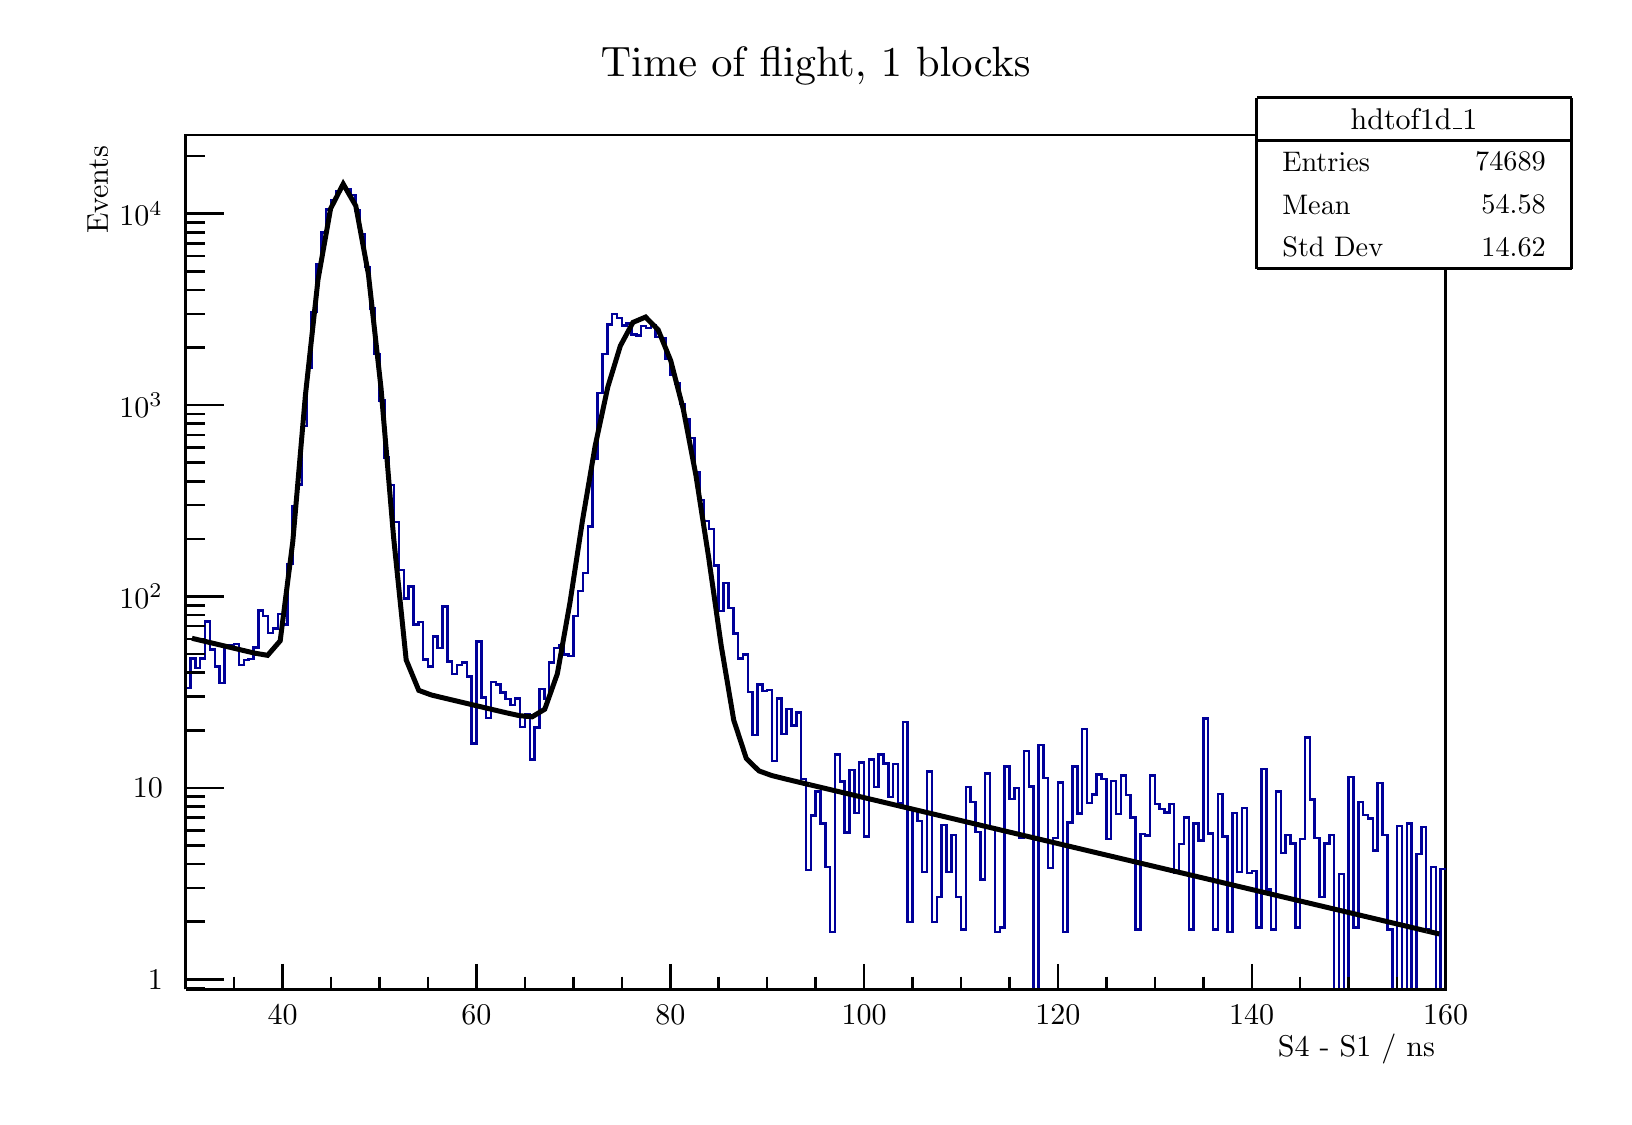
\begin{tikzpicture}
\pgfdeclareplotmark{cross} {
\pgfpathmoveto{\pgfpoint{-0.3\pgfplotmarksize}{\pgfplotmarksize}}
\pgfpathlineto{\pgfpoint{+0.3\pgfplotmarksize}{\pgfplotmarksize}}
\pgfpathlineto{\pgfpoint{+0.3\pgfplotmarksize}{0.3\pgfplotmarksize}}
\pgfpathlineto{\pgfpoint{+1\pgfplotmarksize}{0.3\pgfplotmarksize}}
\pgfpathlineto{\pgfpoint{+1\pgfplotmarksize}{-0.3\pgfplotmarksize}}
\pgfpathlineto{\pgfpoint{+0.3\pgfplotmarksize}{-0.3\pgfplotmarksize}}
\pgfpathlineto{\pgfpoint{+0.3\pgfplotmarksize}{-1.\pgfplotmarksize}}
\pgfpathlineto{\pgfpoint{-0.3\pgfplotmarksize}{-1.\pgfplotmarksize}}
\pgfpathlineto{\pgfpoint{-0.3\pgfplotmarksize}{-0.3\pgfplotmarksize}}
\pgfpathlineto{\pgfpoint{-1.\pgfplotmarksize}{-0.3\pgfplotmarksize}}
\pgfpathlineto{\pgfpoint{-1.\pgfplotmarksize}{0.3\pgfplotmarksize}}
\pgfpathlineto{\pgfpoint{-0.3\pgfplotmarksize}{0.3\pgfplotmarksize}}
\pgfpathclose
\pgfusepathqstroke
}
\pgfdeclareplotmark{cross*} {
\pgfpathmoveto{\pgfpoint{-0.3\pgfplotmarksize}{\pgfplotmarksize}}
\pgfpathlineto{\pgfpoint{+0.3\pgfplotmarksize}{\pgfplotmarksize}}
\pgfpathlineto{\pgfpoint{+0.3\pgfplotmarksize}{0.3\pgfplotmarksize}}
\pgfpathlineto{\pgfpoint{+1\pgfplotmarksize}{0.3\pgfplotmarksize}}
\pgfpathlineto{\pgfpoint{+1\pgfplotmarksize}{-0.3\pgfplotmarksize}}
\pgfpathlineto{\pgfpoint{+0.3\pgfplotmarksize}{-0.3\pgfplotmarksize}}
\pgfpathlineto{\pgfpoint{+0.3\pgfplotmarksize}{-1.\pgfplotmarksize}}
\pgfpathlineto{\pgfpoint{-0.3\pgfplotmarksize}{-1.\pgfplotmarksize}}
\pgfpathlineto{\pgfpoint{-0.3\pgfplotmarksize}{-0.3\pgfplotmarksize}}
\pgfpathlineto{\pgfpoint{-1.\pgfplotmarksize}{-0.3\pgfplotmarksize}}
\pgfpathlineto{\pgfpoint{-1.\pgfplotmarksize}{0.3\pgfplotmarksize}}
\pgfpathlineto{\pgfpoint{-0.3\pgfplotmarksize}{0.3\pgfplotmarksize}}
\pgfpathclose
\pgfusepathqfillstroke
}
\pgfdeclareplotmark{newstar} {
\pgfpathmoveto{\pgfqpoint{0pt}{\pgfplotmarksize}}
\pgfpathlineto{\pgfqpointpolar{44}{0.5\pgfplotmarksize}}
\pgfpathlineto{\pgfqpointpolar{18}{\pgfplotmarksize}}
\pgfpathlineto{\pgfqpointpolar{-20}{0.5\pgfplotmarksize}}
\pgfpathlineto{\pgfqpointpolar{-54}{\pgfplotmarksize}}
\pgfpathlineto{\pgfqpointpolar{-90}{0.5\pgfplotmarksize}}
\pgfpathlineto{\pgfqpointpolar{234}{\pgfplotmarksize}}
\pgfpathlineto{\pgfqpointpolar{198}{0.5\pgfplotmarksize}}
\pgfpathlineto{\pgfqpointpolar{162}{\pgfplotmarksize}}
\pgfpathlineto{\pgfqpointpolar{134}{0.5\pgfplotmarksize}}
\pgfpathclose
\pgfusepathqstroke
}
\pgfdeclareplotmark{newstar*} {
\pgfpathmoveto{\pgfqpoint{0pt}{\pgfplotmarksize}}
\pgfpathlineto{\pgfqpointpolar{44}{0.5\pgfplotmarksize}}
\pgfpathlineto{\pgfqpointpolar{18}{\pgfplotmarksize}}
\pgfpathlineto{\pgfqpointpolar{-20}{0.5\pgfplotmarksize}}
\pgfpathlineto{\pgfqpointpolar{-54}{\pgfplotmarksize}}
\pgfpathlineto{\pgfqpointpolar{-90}{0.5\pgfplotmarksize}}
\pgfpathlineto{\pgfqpointpolar{234}{\pgfplotmarksize}}
\pgfpathlineto{\pgfqpointpolar{198}{0.5\pgfplotmarksize}}
\pgfpathlineto{\pgfqpointpolar{162}{\pgfplotmarksize}}
\pgfpathlineto{\pgfqpointpolar{134}{0.5\pgfplotmarksize}}
\pgfpathclose
\pgfusepathqfillstroke
}
\definecolor{c}{rgb}{1,1,1};
\draw [color=c, fill=c] (0,0) rectangle (20,13.5632);
\draw [color=c, fill=c] (2,1.35632) rectangle (18,12.2069);
\definecolor{c}{rgb}{0,0,0};
\draw [c,line width=0.9] (2,1.35632) -- (2,12.2069) -- (18,12.2069) -- (18,1.35632) -- (2,1.35632);
\definecolor{c}{rgb}{1,1,1};
\draw [color=c, fill=c] (2,1.35632) rectangle (18,12.2069);
\definecolor{c}{rgb}{0,0,0};
\draw [c,line width=0.9] (2,1.35632) -- (2,12.2069) -- (18,12.2069) -- (18,1.35632) -- (2,1.35632);
\definecolor{c}{rgb}{0,0,0.6};
\draw [c,line width=0.9] (2,5.18151) -- (2.06154,5.18151) -- (2.06154,5.55608) -- (2.12308,5.55608) -- (2.12308,5.43961) -- (2.18462,5.43961) -- (2.18462,5.55581) -- (2.24615,5.55581) -- (2.24615,6.03099) -- (2.30769,6.03099) -- (2.30769,5.671) --
 (2.36923,5.671) -- (2.36923,5.45689) -- (2.43077,5.45689) -- (2.43077,5.24567) -- (2.49231,5.24567) -- (2.49231,5.73078) -- (2.55385,5.73078) -- (2.55385,5.72665) -- (2.61538,5.72665) -- (2.61538,5.74226) -- (2.67692,5.74226) -- (2.67692,5.47851) --
 (2.73846,5.47851) -- (2.73846,5.53808) -- (2.8,5.53808) -- (2.8,5.54976) -- (2.86154,5.54976) -- (2.86154,5.69856) -- (2.92308,5.69856) -- (2.92308,6.16999) -- (2.98462,6.16999) -- (2.98462,6.10032) -- (3.04615,6.10032) -- (3.04615,5.88449) --
 (3.10769,5.88449) -- (3.10769,5.93992) -- (3.16923,5.93992) -- (3.16923,6.12156) -- (3.23077,6.12156) -- (3.23077,5.99356) -- (3.29231,5.99356) -- (3.29231,6.75831) -- (3.35385,6.75831) -- (3.35385,7.49725) -- (3.41538,7.49725) -- (3.41538,7.76618)
 -- (3.47692,7.76618) -- (3.47692,8.5123) -- (3.53846,8.5123) -- (3.53846,9.25065) -- (3.6,9.25065) -- (3.6,9.95823) -- (3.66154,9.95823) -- (3.66154,10.5598) -- (3.72308,10.5598) -- (3.72308,10.9657) -- (3.78462,10.9657) -- (3.78462,11.2595) --
 (3.84615,11.2595) -- (3.84615,11.3826) -- (3.90769,11.3826) -- (3.90769,11.4937) -- (3.96923,11.4937) -- (3.96923,11.5322) -- (4.03077,11.5322) -- (4.03077,11.5125) -- (4.09231,11.5125) -- (4.09231,11.4476) -- (4.15385,11.4476) -- (4.15385,11.2503)
 -- (4.21538,11.2503) -- (4.21538,10.9505) -- (4.27692,10.9505) -- (4.27692,10.5305) -- (4.33846,10.5305) -- (4.33846,10.0019) -- (4.4,10.0019) -- (4.4,9.42602) -- (4.46154,9.42602) -- (4.46154,8.83371) -- (4.52308,8.83371) -- (4.52308,8.11005) --
 (4.58462,8.11005) -- (4.58462,7.76378) -- (4.64615,7.76378) -- (4.64615,7.29171) -- (4.70769,7.29171) -- (4.70769,6.67972) -- (4.76923,6.67972) -- (4.76923,6.32169) -- (4.83077,6.32169) -- (4.83077,6.47204) -- (4.89231,6.47204) -- (4.89231,5.993) --
 (4.95385,5.993) -- (4.95385,6.02017) -- (5.01538,6.02017) -- (5.01538,5.54748) -- (5.07692,5.54748) -- (5.07692,5.45714) -- (5.13846,5.45714) -- (5.13846,5.83864) -- (5.2,5.83864) -- (5.2,5.69096) -- (5.26154,5.69096) -- (5.26154,6.21606) --
 (5.32308,6.21606) -- (5.32308,5.51754) -- (5.38462,5.51754) -- (5.38462,5.35984) -- (5.44615,5.35984) -- (5.44615,5.47524) -- (5.50769,5.47524) -- (5.50769,5.50812) -- (5.56923,5.50812) -- (5.56923,5.32886) -- (5.63077,5.32886) -- (5.63077,4.47719)
 -- (5.69231,4.47719) -- (5.69231,5.77627) -- (5.75385,5.77627) -- (5.75385,5.06195) -- (5.81538,5.06195) -- (5.81538,4.80233) -- (5.87692,4.80233) -- (5.87692,5.25956) -- (5.93846,5.25956) -- (5.93846,5.22936) -- (6,5.22936) -- (6,5.12667) --
 (6.06154,5.12667) -- (6.06154,5.04604) -- (6.12308,5.04604) -- (6.12308,4.96718) -- (6.18462,4.96718) -- (6.18462,5.05252) -- (6.24615,5.05252) -- (6.24615,4.68623) -- (6.30769,4.68623) -- (6.30769,4.85157) -- (6.36923,4.85157) -- (6.36923,4.2741)
 -- (6.43077,4.2741) -- (6.43077,4.68523) -- (6.49231,4.68523) -- (6.49231,5.16964) -- (6.55385,5.16964) -- (6.55385,5.0443) -- (6.61538,5.0443) -- (6.61538,5.50863) -- (6.67692,5.50863) -- (6.67692,5.68975) -- (6.73846,5.68975) -- (6.73846,5.72166)
 -- (6.8,5.72166) -- (6.8,5.60763) -- (6.86154,5.60763) -- (6.86154,5.58722) -- (6.92308,5.58722) -- (6.92308,6.09935) -- (6.98462,6.09935) -- (6.98462,6.41753) -- (7.04615,6.41753) -- (7.04615,6.64659) -- (7.10769,6.64659) -- (7.10769,7.2355) --
 (7.16923,7.2355) -- (7.16923,8.09892) -- (7.23077,8.09892) -- (7.23077,8.93136) -- (7.29231,8.93136) -- (7.29231,9.42351) -- (7.35385,9.42351) -- (7.35385,9.79794) -- (7.41538,9.79794) -- (7.41538,9.93183) -- (7.47692,9.93183) -- (7.47692,9.8799) --
 (7.53846,9.8799) -- (7.53846,9.78722) -- (7.6,9.78722) -- (7.6,9.81608) -- (7.66154,9.81608) -- (7.66154,9.67331) -- (7.72308,9.67331) -- (7.72308,9.65902) -- (7.78462,9.65902) -- (7.78462,9.77948) -- (7.84615,9.77948) -- (7.84615,9.75876) --
 (7.90769,9.75876) -- (7.90769,9.79026) -- (7.96923,9.79026) -- (7.96923,9.64053) -- (8.03077,9.64053) -- (8.03077,9.63187) -- (8.09231,9.63187) -- (8.09231,9.36831) -- (8.15385,9.36831) -- (8.15385,9.16368) -- (8.21538,9.16368) -- (8.21538,9.05403)
 -- (8.27692,9.05403) -- (8.27692,8.78876) -- (8.33846,8.78876) -- (8.33846,8.603) -- (8.4,8.603) -- (8.4,8.35968) -- (8.46154,8.35968) -- (8.46154,7.91883) -- (8.52308,7.91883) -- (8.52308,7.56846) -- (8.58462,7.56846) -- (8.58462,7.30407) --
 (8.64615,7.30407) -- (8.64615,7.20532) -- (8.70769,7.20532) -- (8.70769,6.74177) -- (8.76923,6.74177) -- (8.76923,6.16352) -- (8.83077,6.16352) -- (8.83077,6.51821) -- (8.89231,6.51821) -- (8.89231,6.20221) -- (8.95385,6.20221) -- (8.95385,5.87638)
 -- (9.01538,5.87638) -- (9.01538,5.55625) -- (9.07692,5.55625) -- (9.07692,5.61066) -- (9.13846,5.61066) -- (9.13846,5.13328) -- (9.2,5.13328) -- (9.2,4.58783) -- (9.26154,4.58783) -- (9.26154,5.23012) -- (9.32308,5.23012) -- (9.32308,5.146) --
 (9.38461,5.146) -- (9.38461,5.15776) -- (9.44615,5.15776) -- (9.44615,4.25767) -- (9.50769,4.25767) -- (9.50769,5.04774) -- (9.56923,5.04774) -- (9.56923,4.60175) -- (9.63077,4.60175) -- (9.63077,4.92009) -- (9.69231,4.92009) -- (9.69231,4.71042) --
 (9.75385,4.71042) -- (9.75385,4.87061) -- (9.81538,4.87061) -- (9.81538,4.02592) -- (9.87692,4.02592) -- (9.87692,2.87449) -- (9.93846,2.87449) -- (9.93846,3.56693) -- (10,3.56693) -- (10,3.87246) -- (10.0615,3.87246) -- (10.0615,3.4613) --
 (10.1231,3.4613) -- (10.1231,2.90853) -- (10.1846,2.90853) -- (10.1846,2.08809) -- (10.2462,2.08809) -- (10.2462,4.33668) -- (10.3077,4.33668) -- (10.3077,3.99697) -- (10.3692,3.99697) -- (10.3692,3.3477) -- (10.4308,3.3477) -- (10.4308,4.13973) --
 (10.4923,4.13973) -- (10.4923,3.59781) -- (10.5538,3.59781) -- (10.5538,4.23774) -- (10.6154,4.23774) -- (10.6154,3.29987) -- (10.6769,3.29987) -- (10.6769,4.27622) -- (10.7385,4.27622) -- (10.7385,3.92545) -- (10.8,3.92545) -- (10.8,4.34213) --
 (10.8615,4.34213) -- (10.8615,4.22691) -- (10.9231,4.22691) -- (10.9231,3.79686) -- (10.9846,3.79686) -- (10.9846,4.22057) -- (11.0462,4.22057) -- (11.0462,3.71905) -- (11.1077,3.71905) -- (11.1077,4.75094) -- (11.1692,4.75094) -- (11.1692,2.20974)
 -- (11.2308,2.20974) -- (11.2308,3.65017) -- (11.2923,3.65017) -- (11.2923,3.492) -- (11.3538,3.492) -- (11.3538,2.84753) -- (11.4154,2.84753) -- (11.4154,4.12337) -- (11.4769,4.12337) -- (11.4769,2.20974) -- (11.5385,2.20974) -- (11.5385,2.53059)
 -- (11.6,2.53059) -- (11.6,3.44296) -- (11.6615,3.44296) -- (11.6615,2.84753) -- (11.7231,2.84753) -- (11.7231,3.31942) -- (11.7846,3.31942) -- (11.7846,2.53059) -- (11.8462,2.53059) -- (11.8462,2.11846) -- (11.9077,2.11846) -- (11.9077,3.92545) --
 (11.9692,3.92545) -- (11.9692,3.73625) -- (12.0308,3.73625) -- (12.0308,3.35377) -- (12.0923,3.35377) -- (12.0923,2.74928) -- (12.1538,2.74928) -- (12.1538,4.09554) -- (12.2154,4.09554) -- (12.2154,3.41687) -- (12.2769,3.41687) -- (12.2769,2.08809)
 -- (12.3385,2.08809) -- (12.3385,2.14272) -- (12.4,2.14272) -- (12.4,4.18641) -- (12.4615,4.18641) -- (12.4615,3.77723) -- (12.5231,3.77723) -- (12.5231,3.91398) -- (12.5846,3.91398) -- (12.5846,3.27829) -- (12.6462,3.27829) -- (12.6462,4.38363) --
 (12.7077,4.38363) -- (12.7077,3.93124) -- (12.7692,3.93124) -- (12.7692,1.35632) -- (12.8308,1.35632) -- (12.8308,4.45728) -- (12.8923,4.45728) -- (12.8923,4.04146) -- (12.9538,4.04146) -- (12.9538,2.89686) -- (13.0154,2.89686) -- (13.0154,3.27649)
 -- (13.0769,3.27649) -- (13.0769,3.98168) -- (13.1385,3.98168) -- (13.1385,2.08809) -- (13.2,2.08809) -- (13.2,3.47404) -- (13.2615,3.47404) -- (13.2615,4.18641) -- (13.3231,4.18641) -- (13.3231,3.58812) -- (13.3846,3.58812) -- (13.3846,4.66074) --
 (13.4462,4.66074) -- (13.4462,3.72096) -- (13.5077,3.72096) -- (13.5077,3.83058) -- (13.5692,3.83058) -- (13.5692,4.08766) -- (13.6308,4.08766) -- (13.6308,4.03023) -- (13.6923,4.03023) -- (13.6923,3.26645) -- (13.7538,3.26645) -- (13.7538,4.00415)
 -- (13.8154,4.00415) -- (13.8154,3.58678) -- (13.8769,3.58678) -- (13.8769,4.07563) -- (13.9385,4.07563) -- (13.9385,3.82377) -- (14,3.82377) -- (14,3.53914) -- (14.0615,3.53914) -- (14.0615,2.11846) -- (14.1231,2.11846) -- (14.1231,3.33056) --
 (14.1846,3.33056) -- (14.1846,3.3096) -- (14.2462,3.3096) -- (14.2462,4.07579) -- (14.3077,4.07579) -- (14.3077,3.70785) -- (14.3692,3.70785) -- (14.3692,3.64917) -- (14.4308,3.64917) -- (14.4308,3.60516) -- (14.4923,3.60516) -- (14.4923,3.70785) --
 (14.5538,3.70785) -- (14.5538,2.83516) -- (14.6154,2.83516) -- (14.6154,3.20139) -- (14.6769,3.20139) -- (14.6769,3.53914) -- (14.7385,3.53914) -- (14.7385,2.11846) -- (14.8,2.11846) -- (14.8,3.46572) -- (14.8615,3.46572) -- (14.8615,3.24538) --
 (14.9231,3.24538) -- (14.9231,4.79484) -- (14.9846,4.79484) -- (14.9846,3.33729) -- (15.0462,3.33729) -- (15.0462,2.11846) -- (15.1077,2.11846) -- (15.1077,3.83614) -- (15.1692,3.83614) -- (15.1692,3.29647) -- (15.2308,3.29647) -- (15.2308,2.08809)
 -- (15.2923,2.08809) -- (15.2923,3.59713) -- (15.3538,3.59713) -- (15.3538,2.85023) -- (15.4154,2.85023) -- (15.4154,3.66286) -- (15.4769,3.66286) -- (15.4769,2.83516) -- (15.5385,2.83516) -- (15.5385,2.86243) -- (15.6,2.86243) -- (15.6,2.14272) --
 (15.6615,2.14272) -- (15.6615,4.15383) -- (15.7231,4.15383) -- (15.7231,2.62199) -- (15.7846,2.62199) -- (15.7846,2.11846) -- (15.8462,2.11846) -- (15.8462,3.87165) -- (15.9077,3.87165) -- (15.9077,3.08614) -- (15.9692,3.08614) -- (15.9692,3.31751)
 -- (16.0308,3.31751) -- (16.0308,3.21207) -- (16.0923,3.21207) -- (16.0923,2.14272) -- (16.1538,2.14272) -- (16.1538,3.26826) -- (16.2154,3.26826) -- (16.2154,4.55325) -- (16.2769,4.55325) -- (16.2769,3.77087) -- (16.3385,3.77087) --
 (16.3385,3.27829) -- (16.4,3.27829) -- (16.4,2.53059) -- (16.4615,2.53059) -- (16.4615,3.21207) -- (16.5231,3.21207) -- (16.5231,3.31751) -- (16.5846,3.31751) -- (16.5846,1.35632) -- (16.6462,1.35632) -- (16.6462,2.81986) -- (16.7077,2.81986) --
 (16.7077,1.35632) -- (16.7692,1.35632) -- (16.7692,4.05445) -- (16.8308,4.05445) -- (16.8308,2.14272) -- (16.8923,2.14272) -- (16.8923,3.7376) -- (16.9538,3.7376) -- (16.9538,3.57313) -- (17.0154,3.57313) -- (17.0154,3.52486) -- (17.0769,3.52486) --
 (17.0769,3.12021) -- (17.1385,3.12021) -- (17.1385,3.98035) -- (17.2,3.98035) -- (17.2,3.31751) -- (17.2615,3.31751) -- (17.2615,2.11846) -- (17.3231,2.11846) -- (17.3231,1.35632) -- (17.3846,1.35632) -- (17.3846,3.43423) -- (17.4462,3.43423) --
 (17.4462,1.35632) -- (17.5077,1.35632) -- (17.5077,3.4613) -- (17.5692,3.4613) -- (17.5692,1.35632) -- (17.6308,1.35632) -- (17.6308,3.07628) -- (17.6923,3.07628) -- (17.6923,3.41932) -- (17.7538,3.41932) -- (17.7538,2.11846) -- (17.8154,2.11846) --
 (17.8154,2.90853) -- (17.8769,2.90853) -- (17.8769,1.35632) -- (17.9385,1.35632) -- (17.9385,2.88244) -- (18,2.88244);
\definecolor{c}{rgb}{0,0,0};
\draw [c,line width=0.9] (2,1.35632) -- (18,1.35632);
\draw [anchor= east] (18,0.596782) node[scale=1.08496, color=c, rotate=0]{ S4 - S1 / ns};
\draw [c,line width=0.9] (3.23077,1.68184) -- (3.23077,1.35632);
\draw [c,line width=0.9] (3.84615,1.51908) -- (3.84615,1.35632);
\draw [c,line width=0.9] (4.46154,1.51908) -- (4.46154,1.35632);
\draw [c,line width=0.9] (5.07692,1.51908) -- (5.07692,1.35632);
\draw [c,line width=0.9] (5.69231,1.68184) -- (5.69231,1.35632);
\draw [c,line width=0.9] (6.30769,1.51908) -- (6.30769,1.35632);
\draw [c,line width=0.9] (6.92308,1.51908) -- (6.92308,1.35632);
\draw [c,line width=0.9] (7.53846,1.51908) -- (7.53846,1.35632);
\draw [c,line width=0.9] (8.15385,1.68184) -- (8.15385,1.35632);
\draw [c,line width=0.9] (8.76923,1.51908) -- (8.76923,1.35632);
\draw [c,line width=0.9] (9.38461,1.51908) -- (9.38461,1.35632);
\draw [c,line width=0.9] (10,1.51908) -- (10,1.35632);
\draw [c,line width=0.9] (10.6154,1.68184) -- (10.6154,1.35632);
\draw [c,line width=0.9] (11.2308,1.51908) -- (11.2308,1.35632);
\draw [c,line width=0.9] (11.8462,1.51908) -- (11.8462,1.35632);
\draw [c,line width=0.9] (12.4615,1.51908) -- (12.4615,1.35632);
\draw [c,line width=0.9] (13.0769,1.68184) -- (13.0769,1.35632);
\draw [c,line width=0.9] (13.6923,1.51908) -- (13.6923,1.35632);
\draw [c,line width=0.9] (14.3077,1.51908) -- (14.3077,1.35632);
\draw [c,line width=0.9] (14.9231,1.51908) -- (14.9231,1.35632);
\draw [c,line width=0.9] (15.5385,1.68184) -- (15.5385,1.35632);
\draw [c,line width=0.9] (16.1538,1.51908) -- (16.1538,1.35632);
\draw [c,line width=0.9] (16.7692,1.51908) -- (16.7692,1.35632);
\draw [c,line width=0.9] (17.3846,1.51908) -- (17.3846,1.35632);
\draw [c,line width=0.9] (18,1.68184) -- (18,1.35632);
\draw [c,line width=0.9] (3.23077,1.68184) -- (3.23077,1.35632);
\draw [c,line width=0.9] (2.61538,1.51908) -- (2.61538,1.35632);
\draw [c,line width=0.9] (2,1.51908) -- (2,1.35632);
\draw [anchor=base] (3.23077,0.908736) node[scale=1.08496, color=c, rotate=0]{40};
\draw [anchor=base] (5.69231,0.908736) node[scale=1.08496, color=c, rotate=0]{60};
\draw [anchor=base] (8.15385,0.908736) node[scale=1.08496, color=c, rotate=0]{80};
\draw [anchor=base] (10.6154,0.908736) node[scale=1.08496, color=c, rotate=0]{100};
\draw [anchor=base] (13.0769,0.908736) node[scale=1.08496, color=c, rotate=0]{120};
\draw [anchor=base] (15.5385,0.908736) node[scale=1.08496, color=c, rotate=0]{140};
\draw [anchor=base] (18,0.908736) node[scale=1.08496, color=c, rotate=0]{160};
\draw [c,line width=0.9] (2,1.35632) -- (2,12.2069);
\draw [anchor= east] (0.88,12.2069) node[scale=1.08496, color=c, rotate=90]{ Events};
\draw [c,line width=0.9] (2.24,1.37274) -- (2,1.37274);
\draw [c,line width=0.9] (2.48,1.48397) -- (2,1.48397);
\draw [anchor= east] (1.844,1.48397) node[scale=1.08496, color=c, rotate=0]{1};
\draw [c,line width=0.9] (2.24,2.21574) -- (2,2.21574);
\draw [c,line width=0.9] (2.24,2.6438) -- (2,2.6438);
\draw [c,line width=0.9] (2.24,2.94751) -- (2,2.94751);
\draw [c,line width=0.9] (2.24,3.18309) -- (2,3.18309);
\draw [c,line width=0.9] (2.24,3.37557) -- (2,3.37557);
\draw [c,line width=0.9] (2.24,3.53831) -- (2,3.53831);
\draw [c,line width=0.9] (2.24,3.67928) -- (2,3.67928);
\draw [c,line width=0.9] (2.24,3.80363) -- (2,3.80363);
\draw [c,line width=0.9] (2.48,3.91486) -- (2,3.91486);
\draw [anchor= east] (1.844,3.91486) node[scale=1.08496, color=c, rotate=0]{10};
\draw [c,line width=0.9] (2.24,4.64663) -- (2,4.64663);
\draw [c,line width=0.9] (2.24,5.07469) -- (2,5.07469);
\draw [c,line width=0.9] (2.24,5.3784) -- (2,5.3784);
\draw [c,line width=0.9] (2.24,5.61398) -- (2,5.61398);
\draw [c,line width=0.9] (2.24,5.80646) -- (2,5.80646);
\draw [c,line width=0.9] (2.24,5.9692) -- (2,5.9692);
\draw [c,line width=0.9] (2.24,6.11017) -- (2,6.11017);
\draw [c,line width=0.9] (2.24,6.23452) -- (2,6.23452);
\draw [c,line width=0.9] (2.48,6.34575) -- (2,6.34575);
\draw [anchor= east] (1.844,6.34575) node[scale=1.08496, color=c, rotate=0]{$10^{2}$};
\draw [c,line width=0.9] (2.24,7.07752) -- (2,7.07752);
\draw [c,line width=0.9] (2.24,7.50558) -- (2,7.50558);
\draw [c,line width=0.9] (2.24,7.80929) -- (2,7.80929);
\draw [c,line width=0.9] (2.24,8.04487) -- (2,8.04487);
\draw [c,line width=0.9] (2.24,8.23735) -- (2,8.23735);
\draw [c,line width=0.9] (2.24,8.40009) -- (2,8.40009);
\draw [c,line width=0.9] (2.24,8.54106) -- (2,8.54106);
\draw [c,line width=0.9] (2.24,8.66541) -- (2,8.66541);
\draw [c,line width=0.9] (2.48,8.77664) -- (2,8.77664);
\draw [anchor= east] (1.844,8.77664) node[scale=1.08496, color=c, rotate=0]{$10^{3}$};
\draw [c,line width=0.9] (2.24,9.50841) -- (2,9.50841);
\draw [c,line width=0.9] (2.24,9.93647) -- (2,9.93647);
\draw [c,line width=0.9] (2.24,10.2402) -- (2,10.2402);
\draw [c,line width=0.9] (2.24,10.4758) -- (2,10.4758);
\draw [c,line width=0.9] (2.24,10.6682) -- (2,10.6682);
\draw [c,line width=0.9] (2.24,10.831) -- (2,10.831);
\draw [c,line width=0.9] (2.24,10.9719) -- (2,10.9719);
\draw [c,line width=0.9] (2.24,11.0963) -- (2,11.0963);
\draw [c,line width=0.9] (2.48,11.2075) -- (2,11.2075);
\draw [anchor= east] (1.844,11.2075) node[scale=1.08496, color=c, rotate=0]{$10^{4}$};
\draw [c,line width=0.9] (2.24,11.9393) -- (2,11.9393);
\definecolor{c}{rgb}{1,1,1};
\draw [color=c, fill=c] (15.6,10.5115) rectangle (19.6,12.6816);
\definecolor{c}{rgb}{0,0,0};
\draw [c,line width=0.9] (15.6,10.5115) -- (19.6,10.5115);
\draw [c,line width=0.9] (19.6,10.5115) -- (19.6,12.6816);
\draw [c,line width=0.9] (19.6,12.6816) -- (15.6,12.6816);
\draw [c,line width=0.9] (15.6,12.6816) -- (15.6,10.5115);
\draw (17.6,12.4103) node[scale=1.08496, color=c, rotate=0]{hdtof1d\_1};
\draw [c,line width=0.9] (15.6,12.1391) -- (19.6,12.1391);
\draw [anchor= west] (15.8,11.8678) node[scale=1.02114, color=c, rotate=0]{Entries };
\draw [anchor= east] (19.4,11.8678) node[scale=1.02114, color=c, rotate=0]{ 74689};
\draw [anchor= west] (15.8,11.3253) node[scale=1.02114, color=c, rotate=0]{Mean  };
\draw [anchor= east] (19.4,11.3253) node[scale=1.02114, color=c, rotate=0]{  54.58};
\draw [anchor= west] (15.8,10.7828) node[scale=1.02114, color=c, rotate=0]{Std Dev   };
\draw [anchor= east] (19.4,10.7828) node[scale=1.02114, color=c, rotate=0]{  14.62};
\draw [c,line width=1.8] (2.08,5.81522) -- (2.24,5.77729) -- (2.4,5.73936) -- (2.56,5.70143) -- (2.72,5.6635) -- (2.88,5.62584) -- (3.04,5.59883) -- (3.2,5.783) -- (3.36,7.04462) -- (3.52,8.89992) -- (3.68,10.3694) -- (3.84,11.2716) -- (4,11.5852) --
 (4.16,11.3072) -- (4.32,10.4394) -- (4.48,8.9965) -- (4.64,7.0994) -- (4.8,5.54055) -- (4.96,5.1535) -- (5.12,5.09513) -- (5.28,5.05662) -- (5.44,5.01869) -- (5.6,4.98076) -- (5.76,4.94283) -- (5.92,4.90492) -- (6.08,4.86731) -- (6.24,4.83246) --
 (6.4,4.81808) -- (6.56,4.91497) -- (6.72,5.3653) -- (6.88,6.26787) -- (7.04,7.31709) -- (7.2,8.25867) -- (7.36,9.00435) -- (7.52,9.52953) -- (7.68,9.82711) -- (7.84,9.89492) -- (8,9.73249) -- (8.16,9.34039) -- (8.32,8.721) -- (8.48,7.88215) --
 (8.64,6.85117) -- (8.8,5.72561) -- (8.96,4.77556) -- (9.12,4.2879) -- (9.28,4.13137) -- (9.44,4.0733) -- (9.6,4.03279) -- (9.76,3.9946) -- (9.92,3.95665);
\draw [c,line width=1.8] (9.92,3.95665) -- (10.08,3.91871) -- (10.24,3.88078) -- (10.4,3.84285) -- (10.56,3.80492) -- (10.72,3.76699) -- (10.88,3.72906) -- (11.04,3.69113) -- (11.2,3.6532) -- (11.36,3.61527) -- (11.52,3.57734) -- (11.68,3.53941) --
 (11.84,3.50148) -- (12,3.46355) -- (12.16,3.42562) -- (12.32,3.38769) -- (12.48,3.34976) -- (12.64,3.31183) -- (12.8,3.2739) -- (12.96,3.23597) -- (13.12,3.19804) -- (13.28,3.16011) -- (13.44,3.12218) -- (13.6,3.08425) -- (13.76,3.04632) --
 (13.92,3.00839) -- (14.08,2.97046) -- (14.24,2.93253) -- (14.4,2.8946) -- (14.56,2.85667) -- (14.72,2.81874) -- (14.88,2.78081) -- (15.04,2.74288) -- (15.2,2.70495) -- (15.36,2.66702) -- (15.52,2.62909) -- (15.68,2.59116) -- (15.84,2.55323) --
 (16,2.5153) -- (16.16,2.47737) -- (16.32,2.43944) -- (16.48,2.40151) -- (16.64,2.36358) -- (16.8,2.32565) -- (16.96,2.28772) -- (17.12,2.24979) -- (17.28,2.21186) -- (17.44,2.17393) -- (17.6,2.136) -- (17.76,2.09807);
\draw [c,line width=1.8] (17.76,2.09807) -- (17.92,2.06014);
\draw (10,13.0816) node[scale=1.5317, color=c, rotate=0]{Time of flight, 1 blocks};
\end{tikzpicture}

  \end{adjustbox}
  \caption{Example of the time of flight spectrum observed in $\mathit{S4}$ with a combined signal and background function fitted (shown in black)}
  \label{fig:fitEx}
\end{figure}

To produce the data used in this analysis, an exponential background function is subtracted. 
The parameters for this function are taken from the combined signal and background function.


